% SPDX-License-Identifier: Apache-2.0
% Copyright (c) Contributors to the PhysLight Project.
% Tested with 
%  - texlive-2019
%  - pygments-2.3.1
% make
%  OR
% make lores
%
% alternatively
% xelatex -shell-escape main.tex
% bibtex main
% xelatex -shell-escape main.tex
% xelatex -shell-escape main.tex

% to make pictures (not a very perfect process, tbh)
% use geogebra to make a diagram
%  - to Export choose: export to PGF/TikZ
%    - x units: 1.0, y units: 1.0
%    - setup x/y min/max to include the picture
%       (note this draws on the diagram the part that will be exported)
%    - press Generate PGF/TikZ code
%    - copy-paste the block \begin{tikzpicture} into the document
%    - do adjustments of various kinds of label positioning and formatting

% to install pygments on a mac
% sudo easy_install Pygments

% to make fonts work:
% > cp /usr/home/lukes/.fonts.conf ~/.fonts.conf
% > cp -R ~lukes/fonts ~/fonts
% done :-)

% ifplatform and minted need --shell-escape
% \makeglossaries uses the shell for the glossary stuff
% \makeindex uses the texindy thing for the index
% use bibtex for the bibliography
\documentclass[11pt,a4paper]{report}
\usepackage{ifplatform}

\newif\iffancyfonts
% use this if fancy fonts are available
\fancyfontstrue
% else use this
%\fancyfontsfalse

% used to omit blocks of stuff
\newif\ifomit

% used in the source to skip over minted sections
\newif\ifhasminted % defined later

\usepackage[usenames]{color} %used for font color
\usepackage{amssymb} %maths
\usepackage{amsmath} %maths
\usepackage{mathtools} %maths
%\usepackage[utf8]{inputenc} %useful to type directly diacritic characters

\usepackage{import}

% these have to come before mathspec, unfortunately:
% http://tex.stackexchange.com/questions/85696/what-causes-this-strange-interaction-between-glossaries-and-amsmath
% bibliography configuration
\usepackage[square,comma,sort&compress,nonamebreak]{natbib}
% used for end-of-chapter bibliography in Appendix C: Radiance
\usepackage{multibib}
\newcites{rad}{References}

% glossary and acronyms, has to come after hyperref
% The noidx versions need 4.04, which was released on 08 March 2014.
\makeatletter
\usepackage[acronym,xindy,toc]{glossaries}%
\@ifpackagelater{glossaries}{2014/03/08}{%
    \newcommand\MakeGlossaries{\makenoidxglossaries}
    \newcommand\PrintGlossaries{\printnoidxglossaries}
}{%
    \newcommand\MakeGlossaries{\makeglossaries}
    \newcommand\PrintGlossaries{\printglossaries}
}
\makeatother

\usepackage[xindy]{imakeidx}
% ... up to here for simplicity, but only glossaries needs that, strictly speaking

\usepackage{mathspec} % fontspec + maths support
%\usepackage{fontspec,unicode-math} % for LuaLaTeX, doesn't work too well
\usepackage{xunicode} % xelatex/unicode
\usepackage{xltxtra} % xelatex extra pieces

\usepackage{multirow} % \multirow command in tabular environments
\usepackage[colorlinks=true]{hyperref} % for \url, has to come after amsmath

% use pygments to do syntax highlighting of code
% if pygmentize is not available, just comment this out
\usepackage{minted}
% used in conjunction with minted: mdframed is able to do pagebreaks, and this
% propagates to minted when used inside of an mdframed environment
\usepackage{mdframed}

% tikz/pgf for images
\usepackage{pgf,tikz}
\usetikzlibrary{arrows}
%\usepackage{txfonts,pxfonts}
\usepackage{tcolorbox}

% configure spacing around listing
\usepackage{enumitem}
\setlist{noitemsep}
% for header/footer construction
\usepackage{lastpage}
\usepackage{fancyhdr}
% convenient setup for fonts in section headings
\usepackage{sectsty}
% handling of SI units
\usepackage{siunitx}
% allows crossreferencing and reusing of footnotes using \cref
% see http://tex.stackexchange.com/questions/10102/multiple-references-to-the-same-footnote-with-hyperref-support-is-there-a-bett/10116#10116
\usepackage{cleveref}
\crefformat{footnote}{#2\footnotemark[#1]#3}
% add support for \marginnote
\usepackage{marginnote}
% adjust margins a bit
\ifmacosx
% it seems the sum for bottom (1in+31.5pt) doesn't work for the mac
% but it appears to work fine on linux...
\usepackage[driver=xetex,a4paper,
            top=1in, bottom=1.4in,
            left=1.25in, right=1.25in]{geometry}
\else
\usepackage[driver=xetex, a4paper,
            top=1in, bottom=1.5in,
            left=1.25in, right=1.25in]{geometry}
\fi

% deals with warning: headheight too small from fancyhdr,
% not sure what it's about though
\iffancyfonts
\setlength{\headheight}{31.5pt}
\else
\setlength{\headheight}{15pt}
\fi

% get ourselves some colors
\definecolor{qqwuqq}{rgb}{0,0.39,0}
\definecolor{xdxdff}{rgb}{0.49,0.49,1}
\definecolor{uuuuuu}{rgb}{0.27,0.27,0.27}
\definecolor{eqeqeq}{rgb}{0.88,0.88,0.88}
\definecolor{uuuuuu}{rgb}{0.27,0.27,0.27}
\definecolor{qqqqff}{rgb}{0,0,1}
\definecolor{cqcqcq}{rgb}{0.75,0.75,0.75}
\definecolor{xdxdff}{rgb}{0.49,0.49,1}

% setup colors for links
\definecolor{hyperref-color}{rgb}{0.1,0.1,0.3}
\hypersetup{
  colorlinks,
  citecolor=hyperref-color,
  linkcolor=hyperref-color,
  urlcolor=hyperref-color}

% enable TeX ligatures: `` '' -- --- !` ?` << >>
% works in xelatex but not lualatex
% see http://tex.stackexchange.com/questions/37855/fontspec-with-helvetica-breaks-quotes
\defaultfontfeatures{Ligatures=TeX}

\ExplSyntaxOn
% \NewFontFamily takes the same arguments to \newfontfamily, prepended by
% one to be a name that expands to something that can be passed to \fontfamily
% so that if you have
% \NewFontFamily\foo\foofamily{Ubuntu Mono}
% {\foofamily test}
% and
% {\fontfamily{\foo}\selectfont test}
% are rendered with the same font
\DeclareDocumentCommand \NewFontFamily { m m O{} m }
{
    \newfontfamily #2 [#3] {#4}
    \cs_set_eq:NN #1 \l_fontspec_family_tl
}

% use \Unicode{E1C0} for symbol U+E1C0
% equivalente to \symbol{\string"E1C0}
\DeclareDocumentCommand \Unicode { m }
{
    \symbol{\string"#1}
}
\ExplSyntaxOff

\iffancyfonts
  %\input{warnock_font}
      % define the fonts we like
    % main, serif font
    \setmainfont[
        SizeFeatures={
            {Size={-9},    Font=*},
            {Size={9-13},  Font=*},
            {Size={13-25}, Font=*},
            {Size={25-},   Font=*}
        }
    ]{Crimson Text}
    % in math mode too
    \setmathfont(Digits,Latin,Greek)[
        SizeFeatures={
            {Size={-9},    Font=*},
            {Size={9-13},  Font=*},
            {Size={13-25}, Font=*},
            {Size={25-},   Font=*}
        }
    ]{Crimson Text}
    % for upright set stuff (cos, log)
    \setmathrm[
        SizeFeatures={
            {Size={-9},    Font=*},
            {Size={9-13},  Font=*},
            {Size={13-25}, Font=*},
            {Size={25-},   Font=*}
        }
    ]{Crimson Text}
    % sans serif
    \setsansfont{Noto Sans Light}
    \setmathsf{Noto Sans Light}
    % monospaced
    \setmonofont{Vollkorn}
    \setmathtt{Vollkorn}

  %    % define the fonts we like
    % main, serif font
    \setmainfont[
        SizeFeatures={
            {Size={-9},    Font=* Caption},
            {Size={9-13},  Font=*},
            {Size={13-25}, Font=* Subhead},
            {Size={25-},   Font=* Display}
        }
    ]{Adobe Jenson Pro}
    % in math mode too
    \setmathfont(Digits,Latin,Greek)[
        SizeFeatures={
            {Size={-9},    Font=* Caption},
            {Size={9-13},  Font=*},
            {Size={13-25}, Font=* Subhead},
            {Size={25-},   Font=* Display}
        }
    ]{Adobe Jenson Pro}
    % for upright set stuff (cos, log)
    \setmathrm[
        SizeFeatures={
            {Size={-9},    Font=* Caption},
            {Size={9-13},  Font=*},
            {Size={13-25}, Font=* Subhead},
            {Size={25-},   Font=* Display}
        }
    ]{Adobe Jenson Pro}
    % sans serif
    \setsansfont{Myriad Pro Light}
    \setmathsf{Myriad Pro Light}
    % monospaced
    \setmonofont{Chaparral Pro}
    \setmathtt{Chaparral Pro}

  % for sections titling in sans, black
  \newfontfamily\sectionsFont[LetterSpace=-5]{Noto Sans Black}
  \allsectionsfont{\sf}
  \chapterfont{\sf\sectionsFont}
  \sectionfont{\sf\sectionsFont}
  \partfont{\sf\sectionsFont}

  % for the physLight "logo" font
  \newfontfamily\titleFont[Scale=.9]{Charmonman}
  \def\physLight{{\titleFont p\kern-.075ex h\kern-.075ex y\kern-.075ex sLig\kern-.2ex ht}}

  % for the units
  \NewFontFamily\unitFont\unitFontFamily[Scale=.925]{Vollkorn}

  % for the listings
  \ifmacosx
    \NewFontFamily\mintedFont\mintedFontFamily[Scale=.8]{SF Menlo}
  \else
    \NewFontFamily\mintedFont\mintedFontFamily[Scale=.925]{Noto Sans}
  \fi

\else
  % use vanilla fonts
  \def\physLight{\emph{physLig\kern-.425ex ht}}
  \allsectionsfont{\sf}
\fi

% configure minted
\makeatletter
  \@ifpackageloaded{minted}{\hasmintedtrue}{\hasmintedfalse}
\makeatother

\ifhasminted
  % to check what pygmentize styles are available use
  % pygmentize -L styles
  \usemintedstyle{friendly}
  % redefine \theFancyVerbLine to control the formatting of line numbers
  \definecolor{minted-bg}{rgb}{.95, .95, .95}
  % global options for minted. Language-specific options override document-wide
  % options. Individual command and environment options override
  % language-specific options. The language can be passed as a first optional
  % parameter (\setminted[c++]\{...})
  %\setminted{
  %  bgcolor=minted-bg,
  %  mathescape=true,
  %  texcl=true
  %}
  % cheat: minted is actually a thin wrapper around fancyvrb
  % fvset sets globals for fancyvrb
  \fvset{
    fontfamily=\mintedFont,
    frame=topline,
    framesep=2mm,
    labelposition=topline,
    numbersep=1em,
    samepage=false,
    stepnumber=5,
    tabsize=4
    }
  % we use minted inside an mdframed environment, this is the global
  % configuration for mdframed
  \mdfsetup{
    backgroundcolor=minted-bg,
    linecolor=black,
    topline=false,
    bottomline=false,
    leftline=false,
    rightline=false
  }
  % a command like \newminted, which uses mdframed to work around a page-break
  % limitation that minted has in texlive 2014. Note the minted shipping with
  % texlive 2016+ apparently has this fixed, so this might not be needed after
  % we upgrade
  \newcommand\makemyminted[3]{%
\newenvironment{#1}{\VerbatimEnvironment
\begin{mdframed}
\small
\begin{minted}[mathescape=true,
               texcl=true,
               label=\raisebox{-0.5ex}{#3}]{#2}}
{\end{minted}
\end{mdframed}}}
\else
  \usepackage{fancyvrb}
  \fvset{
    fontfamily=\mintedFont,
    frame=topline,
    framesep=2mm,
    labelposition=topline,
    numbersep=1em,
    samepage=false,
    stepnumber=5,
    tabsize=4
    }
\newcommand\makemyminted[3]{%
\newenvironment{#1}{\VerbatimEnvironment
\begin{mdframed}
\begin{Verbatim}[label=\raisebox{-0.5ex}{#3}]{#2}}
{\end{Verbatim}
\end{mdframed}}}
\fi

% these two need to be implemented in terms of mintinline, after we upgrade
%\def\rsl#1{{\Verb@#1@}}
%\def\rib#1{{\Verb@#1@}}
\makemyminted{pythoncode}{python}{Python}
\makemyminted{c++code}{c++}{C++}
\makemyminted{rslcode}{c++}{RenderMan SL}% pretend it's c++
\makemyminted{ribcode}{text}{RenderMan RIB}% no syntax highlighting
% blocks of text of various kinds
\makemyminted{csvdata}{text}{CSV file}

% there seems to be some odd interaction between fancyfonts and setacronym
\ifdefined\setacronymstyle
  \setacronymstyle{long-sc-short}
\fi
% setup acronyms to be displayed in letterspaced small caps
\renewcommand*{\firstacronymfont}[1]{\textsc{\addfontfeature{LetterSpace=5}#1}}
\renewcommand*{\acronymfont}[1]{\textsc{\addfontfeature{LetterSpace=5}#1}}

% load the glossary into this file
\loadglsentries{glossary}

\MakeGlossaries

% disable the first-use flag for a few well-known acronyms
\glsunset{RGB}
\glsunset{sRGB}
\glsunset{XYZ}

% indices
%  unqualified entries
\makeindex[intoc,title=Index]
%  people
%\makeindex[name=persons,intoc,title=Index of names]


% our version number
\def\physLightVersion{v 1.1 - \today}

% mathbb R, for the real numbers
\def\R{\mathbb{R}}
% wrapper to insert URL's
\def\link#1{{\small\url{#1}}}
% used in tables to make the font small and slanted
\def\smsl{\footnotesize\sl}

% used for product names
\newcommand\productname[1]{\textit{#1}}

\newenvironment{inconstruction}[1][This section is under construction]{
\noindent
\let\oldunitlength\unitlength
\setlength{\unitlength}{.5in}
\begin{minipage}{\unitlength}
\begin{picture}(1,1)
    \put(0,0){
\includegraphics[width=\unitlength]{figures/construction.pdf}}
\end{picture}
\end{minipage}\hfill
\begin{minipage}{\textwidth - \unitlength - 2em}
\vspace{1ex}
\begin{tcolorbox}[colback=green!5!white,colframe=green!75!black,title=#1]


}{
\end{tcolorbox}
\end{minipage}
\let\unitlength\oldunitlength
}

% add a few units and configure unit formatting
% first, the unit symbols are set in their own font family
\iffancyfonts
  \sisetup{
	  unit-math-rm = \unitFontFamily,
   	  unit-text-rm = \unitFontFamily,
  }
\else
  \sisetup{
	  unit-math-rm = \mathtt,
  	  unit-text-rm = \ttfamily,
  }
\fi
\sisetup{
	exponent-product = \cdot, % 1.3\cdot10^3
	inter-unit-product = \ensuremath{{}\cdot{}}, % m\cdot s
	per-mode = symbol-or-fraction, % / in inline mode, \frac in display mode
	power-font = unit, % maybe this should be 'number'?
	%number-unit-product = \text{~}, % per Chicago Manual of Style, I don't like it
	number-unit-product = \ensuremath{\;}, % a little smaller
}
\DeclareSIUnit{\talbot}{Tb}
\DeclareSIUnit{\nit}{nt}
\DeclareSIUnit{\iso}{ISO}
\DeclareSIUnit{\pixel}{pxl}
\DeclareSIUnit{\fnumber}{f-number}
% alternatively we could use cd/m^2
%\def\nit\candela\per\square\meter
% tell PGF about how we want numbers formatted
\SendSettingsToPgf

% configure page headers and footers
%\pagestyle{myheadings}
%\markboth{\hfill  \hfill \physLight}{\physLight \hfill \physLightVersion \hfill}

\pagestyle{fancy}
\lhead{}
\chead{\leftmark}
\rhead{\physLight}
\lfoot{\textit{Weta Digital}}
\cfoot{\textsc{\physLightVersion}}
\rfoot{Page \thepage\,/\,\pageref*{LastPage}}

% thickness of the rules
\renewcommand{\headrulewidth}{.4pt}
\renewcommand{\footrulewidth}{.4pt}

%\includeonly{sec_wcl}

\renewcommand{\d}{\mathop{}\!\mathrm{d}}

\newcommand{\todo}[1]{\begin{tcolorbox}[colback=red!5!white,colframe=red!75!black,title=TODO]{#1}\end{tcolorbox}}

\begin{document}
%\setacronymstyle{long-sc-short}
\begin{titlepage}
\begin{center}

{\fontsize{60}{72}\selectfont \physLight}\\[.3cm]

\textsf{\textit{\fontsize{24}{26.8}\selectfont physical units in light transport}}\\[1.5cm]

\vfill
\large
\textit{Weta Digital Rendering Department}\\[1mm]

% \begin{minipage}{0.4\textwidth}
% \begin{flushleft} \large
% %\emph{Author:}\\
% Luca \textsc{Fascione}\\
% Sehera \textsc{Nawaz}
%
% \end{flushleft}
% \end{minipage}
% \begin{minipage}{0.4\textwidth}
% \begin{flushright} \large
% \textit{Weta Digital Rendering Department}
% \end{flushright}
% \end{minipage}

%\vspace{3mm}
\hrule \vspace{1mm}
\textsc{\large \physLightVersion}\\[0.5cm]

\end{center}
\end{titlepage}

\tableofcontents
\listoffigures
\listoftables
% SPDX-License-Identifier: Apache-2.0
% Copyright (c) Contributors to the PhysLight Project.

\chapter{Notation and symbols}\label{ch:notation}
%\addcontentsline{toc}{chapter}{Notation}

This document makes extensive use of subscripts because we have quantities like 
\emph{flux} that can be measured in several ways (\emph{radiant flux}, \emph{spectral radiant flux},
\emph{luminous flux}, to give examples of quantities we have actually encountered) and we
want to pinpoint which one among these several perspectives we are considering at the present time,
while also suggesting that under a broader strokes perspective these are part of the same
kind of measurement.
This means that these subscripts will apply to several of these quantities: we've seen
\emph{luminous flux}, \emph{luminous energy}, \emph{luminous emittance} for example.
For this reason, in the table that follows, given that we want to draw attention to 
the subscript itself, and not to the specific symbol it happens to be attached to, 
we'll present it attached to an empty square like this: $\square_v$.

Because in this document there are many standard symbols and units sharing the
same symbol, we decided to always keep units inside square brackets to minimize chances of 
confusion. Note that in this respect we deviate from standard practice.

Many, if not the majority of, light transport quantities are actually functions, 
taking as arguments values that represent maybe a given position, or a direction, or a wavelength,
of particular interest, as the case might be. 
Normally we would put these argument to our functions in parentheses, for example in the expression 
$M_e(x)$. 
However in many cases being explicit about these dependencies adds a lot of typed material 
to our equations and ends up making their meaning more obscure because of the many symbols the reader 
has to scan through. 
This is a case where the benefit of added precision undermines what we think is a higher precedence goal
of clarity in communication.
For this reason, we have opted to omit arguments in complex expressions where the surrounding 
text makes it clear what the expression actually means. 
For example we would use expression like $\int f \d x$ in place of
$\int f(x) \d x$, when it's clear that $f$ is in fact a function of $x$.
The discussion of~\cref{eqn:imaging1} is a good example of this practice.

% another possibility is to use labelwidth=\widthof{\bfseries The longest label}
% but this would require us to update with a copy of our longest label
\begin{description}[leftmargin=!,labelwidth={5em}]
\item[ {$\square$} ] a placeholder to indicate the location of some symbol
\item[ {$[\square]$} ] square brackets indicate the contained symbol is a unit,
	brackets will be empty of \emph{pure numbers}
\item[ {$\square^\uparrow$} ] an arrow pointing up $\uparrow$ is used to indicate 
	exitant quantities, that is leaving the object or location
\item[ {$\square^\downarrow$} ] an arrow pointing down $\downarrow$ is used to indicate 
	incident quantities, that is arriving at the object or location

\item[ {$\delta\square$} ] a small, differential amount of $\square$

% our constants and names
\item[{$\Omega$}] a solid angle
\item[{$\omega$}] a direction, usually within the solid angle $\Omega$
\item[$S$] a light source, or the region where its light originates
\item[$R$] a light receiver, or the region where it receives light
\item[{$t\;[\unit\second]$} ] a time period
\item[$k_i$] imaging constant: scale factor between luminous exposure and pixel values
\item[$p^{img}$] location on the filmback or image plane
\item[$W_{pos}(p^{img})$] local response of the filmback
\item[$W_{col}(\lambda)$] spectral response of the filmback
\item[$W(p^{img},\lambda)$] film response function

\item[{$\lambda\;[\unit\meter]$} ] wavelength
\item[{$\nu\;[\unit\hertz]$} ] frequency

% general photography quantities and constants
\item[{$C$}] incident-light meter calibration constant $312.5 = 100 \sfrac{25}8$ for this document
\item[{$f$}] focal length
\item[{$N$}] aperture number
\item[{$o$}] focus distance
\item[{$\Delta t$}] exposure time
\item[{$S$}] film speed
\item[{$T_{cp}$}] \gls{CCT} of a white point
\item[{$N$}] aperture number



% from lighting standard vocabulary
\item[{$N_p\;[]$} ] number of photons
\item[{$Q_p\;[\unit\joule]$} ] energy of one photon
\item[{$Q_e\;[\unit\joule]$} ] radiant energy


% from SI
\item[{$h$} ] Planck's constant (see~\cite{bipm:si.2019})
\item[{$K_{cd}$} ] luminous efficacy of monochromatic radiation (see~\cite{bipm:si.2019})

\item[{$\unit\joule$} ] unit: joule, measures amounts of energy
\item[{$\unit\watt$} ] unit: watt, measures power, being energy per 
	unit of time $[\unit\watt] = [\unit{\joule\per\second}]$
\item[{$\unit\hertz$} ] unit: watt, measures power, being energy per 
	unit of time $[\unit\hertz] = [\unit{1\per\second}]$
\item[{$\unit\radian$} ] 	unit: radian, measures angles
\item[{$\unit\steradian$} ] unit: steradian, measures solid angles
                   
\end{description}

\paragraph{Vector-valued functions and integrals}

\begin{inconstruction}
	Explain the meaning of this expression
	\begin{displaymath}
		\begin{pmatrix}X\\Y\\Z\end{pmatrix}
		= \int_\Lambda S(\lambda)\; 
		\begin{pmatrix}
			\bar x(\lambda)\\
			\bar y(\lambda)\\
			\bar z(\lambda)
		\end{pmatrix}
		\d\lambda
	\end{displaymath}
\end{inconstruction}


\paragraph{Scalar product}

Given two vectors $x,y \in R^n$ we will indicate their components using a
subscript index,
for example for $n=2$ we would have $x = (x_1, x_2)$.
We will write their \textsl{scalar product} using angle bracket notation
$\langle \cdot, \cdot \rangle$:
\begin{displaymath}
\langle x, y \rangle = \sum_{i=1}^n x_i y_i = xy^t,
\end{displaymath}
where the second equality signifies row-vector notation (vectors are thought
of as matrices of one row). Sometimes it's useful to inject an $n\times n$ matrix $M$ ``in the middle''
of a scalar product, defined as follows $\langle x, y \rangle_M := \langle M x, M y \rangle$.

An often useful construct is the following relation: given
three vectors $x,y,z \in \R^n$
\begin{displaymath}
\langle x,y \rangle \langle y,z \rangle
  = \left(x y^t\right)\left(y z^t\right)
  = x \big(y \otimes y\big) z^t
  = \langle x, z\rangle_y
\end{displaymath}
where the symbol $\otimes$ indicates the \textsl{outer product} defined as $x\otimes y :=
x^t y$. Here is an example in $\R^3$:
\begin{displaymath}
x\otimes y =
\left[
\begin{array}{ccc}
x_1 y_1 & x_1 y_2 & x_1 y_3 \\
x_2 y_1 & x_2 y_2 & x_2 y_3 \\
x_3 y_1 & x_3 y_2 & x_3 y_3 \\
\end{array}
\right].
\end{displaymath}


\paragraph{Scalar product of functions}
Given two functions $f,g:X\to\R$ we define their scalar product
$\langle f, g \rangle$ as
\begin{displaymath}
\langle f, g \rangle := \int_X f(x)g(x) \d x, \qquad \langle f, g \rangle_\mu := \int_X f(x)g(x)\mu(x) \d x.
\end{displaymath}

\begin{inconstruction}
	Discuss how scalar product and dot product are connected
	Discuss how scalar product and inner product are connected
	Explain how to integrate a vector-valued function like $W_{\XYZ}(\lambda)$ 
\end{inconstruction}

\paragraph{Norm of a function}
Given a function $f(x): X\to\R$ we will often speak about the integral norm over its
domain $X$, sometimes after weighting with a second positive valued function
$\mu(x): X\to\R^+$, this will be notated as follows
\begin{displaymath}
\|f\| := \int_X |f(x)| \d x, \qquad \|f\|_\mu := \int_X |f(x)| \mu(x) \d x
\end{displaymath}
it is sometimes useful to consider the $p$-norm of a function $f$:
\begin{displaymath}
\|f\|^p := \sqrt[p]{\int_X |f(x)|^p \d x}, \qquad \|f\|_\mu^p := \sqrt[p]{\int_X |f(x)|^p \mu(x)\d x}.
\end{displaymath}

In the case of a function $g(x): X\to\R^n$ we apply the relations above to
each component separately, for example, in the case of $n = 2$ we would have
$g(x) = (g_1(x), g_2(x))$, where $g_1,g_2:X\to\R$
\begin{displaymath}
\|g\|_\mu := \left(\|g_1\|_\mu, \|g_2\|_\mu\right) \in \R^2.
\end{displaymath}


\part{Models \& Specification}\label{part:models}

% SPDX-License-Identifier: Apache-2.0
% Copyright (c) Contributors to the PhysLight Project.

\chapter{Introduction}


\ifomit


color responsivity in XYZ or in camera RGB?
exposure vs density curve plots




test: try the siggraph font styles
test: try Libertine for body text

\fi

\section{Physical units and digital image synthesis}
%
\epigraph{%
	\emph{Pictures shall be based on models built from Euclidean geometry
		in three dimensions, viewed in two dimensions with Renaissance perspective
		and use Newtonian physics. [...] 
		there is nothing about computers or computation that forces these choices}}
		{\textsc{Alvy Ray Smith}, \emph{The Central Dogma}}

\noindent One of the reasons physically-based image synthesis has become such an
indispensable ingredient for pushing realism and consistency in very
complex scenarios is predictability. 
% todo: "what is needed" by whom? for what purpose? Among whom is this "gnerally accepted"?
In fact it is generally assumed that what is needed is an image synthesis system
capable of \emph{photorealism}, that is a system that \emph{given the virtual 
	description of a scene consisting of geometry, material, light sources and cameras
	produce a photorealistic image of it, as if it were captured by a real camera.
	This problem is known as light transport simulation}\footnote{
	This specific phrasing is due to Alexander Rath, during the technical talk at 
	Siggraph 2023 presenting~\cite{rath23}}.
% todo: I'd say "light transport" generally does NOT include "as captured by a real camera," since we usually think of that last step as involving exposure of the emulsion and then the chemistry that follows (for film), or the processing of sensor data, which can include various amplification and filtering steps to compensate for sensor design. I suggest referring to a description of the light falling onto the focal plane of a specific and precisedly-described camera, and leave "capturing" out of it.

Material modelling is based on physical properties and thus allows to reproduce 
increasingly complex natural phenomena. 
% todo: "increasingly complex natural phenomena" is lacking a referent
In traditional rendering systems, before the advent of physically-based light transport, 
control of the look of a material was generally owned by the \gls{shading system}.
The \glspl{shader} would be essentially arbitrary pieces of code in charge of computing
the color of an object at a location requested by the renderer. 
Their programmable nature was used for essentially three purposes:
the first was to compute an object's appearance, for example accessing \emph{texture maps},
the second was to compute how light would interact with the material being modeled, often including
all sorts of approximations to overcome shortcomings in the renderer available at the time 
(for example, missing support for indirect illumination),
the third was to \emph{overdrive} the appearance, taking it beyond what would have been possible in a real-life
counterpart, to achieve various kinds of artistic effects.
% todo: I think of "overdrive" as meaning "amplification by extreme amounts." While shaders can certainly just multiply everything by a number much larger than 1, they can also do far more - really, amost anything. I'd replace "overdrive" (both here and later) with something referring to this opportunity for arbitrary operations.

The physically-based rendering paradigm dictates that \glspl{material model},
lighting and camera response are independent entities and
must hence always be controlled with this separation in mind. 
This makes \gls{virtual} assets more reusable, 
and allows to achieve better consistency when integrating 
digitally produced content with live action \gls{footage}.
This also reduces the scope of the shaders, that end up losing the ability
to \emph{overdrive} and remain more connected to a physically-correct 
model of the world.

Naturally, since a wide range of different effects interplay with each
other in complex and subtle ways, it is absolutely crucial that all
components are accurately represented by their virtual analogues to be
able to reproduce real-world footage realistically. 
Furthermore, the description of the \gls{virtual scene} being based on
real-world quantities enables easier control and verification.




In this document we focus on the specification of \gls{virtual} \glspl{illuminant} and
\glspl{sensor} and make the case for using the same conventions and physical units as
used by lighters and photographers on a motion picture set or in a photographic studio. 
For example, it is preferable in terms of predictability to think about brightness of a 
light source in terms of \glsdisp{photometry}{photometric} units, i.e., units which represent brightness as
perceived by a \gls{human observer}, rather than \glsdisp{radiometry}{radiometric} ones 
(commonly called \gls{wattage}) for two reasons: 
firstly there is convention: the normally used wattage reported on a light fixture or bulb 
is a measure of the power absorbed by the object, not the power of the radiation it emits 
\emph{in the visible range}\footnote{This is effectively the concept of  
	\textsl{\gls{luminous efficacy}}, being the ratio of power absorbed by the emitter
	to the luminous power emitted. 
	What used to be the common household lightbulb, containing incandescent tungsten and 
	rated for 100W, had a luminous efficacy of roughly $15\unit{\lumen\per\watt}$, 
	a contemporary \glsname{LED} lightbulb would be somewhere between 
	$100\unit{\lumen\per\watt}$ and $200\unit{\lumen\per\watt}$, 
	a Xenon arc-lamp somewhere between $30\unit{\lumen\per\watt}$ and
	$90\unit{\lumen\per\watt}$. 
	Note that conservation of energy dictates that when considering all the
	radiation emitted by the bulb, the total radiated power \emph{must} be equal 
	to the absorbed ``electrical'' power, and in fact it's all there: for example for
	tungsten radiators (household lightbulbs) most of the emitted
	photons are infra-red (radiative heat), and the remaining part is distributed in the rest of
	the electromagnetic spectrum} onto the \gls{scene}. 
Secondly, the perceived \gls{brightness} of a source has a fairly marked dependence on 
its color, making lights emitting the same amount of radiative power (even when measured 
limited to the visible spectrum only) appear to have different brightnesses. 
Thirdly, a person's subjective sense of brightness of a source is influenced by all sorts
of contrast or ratio metrics such as the size of the source compared to the visible field,
its brightness compared to other sources in the scene, various forms of eye fatigue accumulated
by the observed and much more. This last group of perception effects is a very big field of
study, covered in books such as \cite{wyszecki82} or \cite{fairchild2013}.

We want instead to specify a system of units and models, in such a manner that
given a real-world scene and a virtual model of it,
specifying the same illuminants via our chosen units, using the same
camera settings and feeding the scene to a compliant renderer will replicate 
the same pixel values as would come from a real-world camera places in the 
real-world version. 
Naturally, for reproducing color, we will not only need
to develop an accurate understanding of brightness, but also be aware
of how \gls{spectral} data flows through the \gls{pipeline}.



The resulting system has been in use in the
production pipeline at \companyname{W\=et\=a FX} since about 2015.
Because of the origin of this system in the motion picture industry,
several terms of the trade have made it into this document. 


The prevalent way of reasoning about image synthesis through rendering is 
built on the notion of the \textsl{light ray}, which is the fundamental element 
of geometrical optics. 
Light rays are the path segments\footnote{
	In the vast majority of renderers in use today, rays are implemented as 
	straight line segments, which enormously simplifies the implementation of the
	code that finds their endpoints. This ignores two effects: the first is that 
	gravity bends light rays and the second it that variations in the index
	of refraction will alter the direction of a light ray.
	Usually bending resulting from gravity won't be an important effect except 
	for scenes that are particularly large and include body with very high mass 
	concentrations like black holes.
	Scenes like this are occasionally rendered, though: for example the 
	movie~\cite{interstellar2014} did need to capture the bending effect of 
	gravity onto light paths accurately, and a specialized rendering system 
	was developed for use on the show. 
	The task was complex enough that the Nobel laureate and CalTech professor 
	Kip Thorne was included as consultant to support the team developing this 
	technology. 
	The second effect ignored by the straight-line approximation is that 
	continuous variations in the index of refraction throughout the volume of a material 
	will bend the light paths into curves. 
	This is a substantially more common effect at human scale, for example 
	it's the origin of the \textsl{mirage} phenomenon. 
	While there are several research projects that have built renderers able 
	to capture this effect, a recent example
	of this kind of work was described in~\cite{fraboni23}, 
	the computational costs associated with this capability 
	are high enough to make it impractical for everyday use.
	Renderers and transport models built on the \emph{wave optics} model also exist,
	a recent example being described in~\cite{yu23}.
	There are several further effects that are generally not captured in 
	light transport simulations for general use, maybe the most prominent of these would be
	polarization, fluorescence and phosphorescence. Of the three, fluorescence
	(the ability of some material to absorb light at one wavelength and re-emit it
	at a different wavelength, typically of lower energy) is a substantial headache for
	a light transport implementation, because it makes it substantially more costly for the 
	engine managing the paths to reason about the path distributions, and account correctly
	for the various probability measures used by the path tracing algorithms
} through space that light follows when traveling across the \gls{virtual scene}. 

This document is divided in parts: \cref{part:models}
contains an introduction on basic quantities that are relevant in
light transport simulation and review the relation of photometric and
radiometric units and describes the modelling aspects. In 
\cref{ch:lighting} we describe imaging and light models and propose the
relevant sets of parameters to specify them accurately.  
\Cref{ch:calcsheets} provides some examples on how to derive some of
the described quantities from real world examples.

\Cref{part:ref} provides a reference covering measurements of various 
illuminants (\cref{ch:illuminants}) and cameras (\cref{ch:sensors}).

\Cref{part:app} contains the appendices: \cref{ch:color} discusses
various considerations on color, in particular covering the relation between 
the tristimulus versus spectral settings,
\cref{ch:implementation} describes an implementation of a color manipulation library
and \cref{ch:radiance} is an extensive excerpt from Frederic Nicodemus's 
excellent 1963 paper~\cite{nicodemus63} in which the concept of \textsl{\gls{radiance}}
is introduced: we found his explanation so clear and elegant that we decided to retype 
his words, with the only change being we have changed the equations to use current 
conventions for quantity names and symbols\footnote{
	The current convention is also a result of Nicodemus's later work,
	about a decade after the original work was published}, 
and adopted \glsname{si} units throughout.

Because this document is the result of work started from the movie industry, 
we are aware several concepts may not be as well known to our readers from different backgrounds. 
For this reasons we have compiled a reference of notation and symbols used in~\cref{ch:notation} 
as well as a glossary in \cref{sec:main} with the hope these might help clarify potential issues arising 
from our use of movie-making jargon.

\section{Quantities in light transport}
\epigraph{%
	\emph{It has been	my experience that most people find it peculiarly difficult to master 
	the fundamental concepts and relations of radiometry (or photometry) as they apply 
	to extended sources. And I have come to believe that the key to this difficulty 
	lies in the interrelated concepts of an elementary beam of radiation and its 
	radiance (or luminance)}}{\textsc{Fred Nicodemus}, 1963}

\noindent We discussed how \gls{rendering} is concerned with simulating how light travels around in 
a \gls{virtual scene}, so this section introduces names for the quantities transported 
along these paths during the simulation and outlines the theory behind them. 
The naming we adopt was originally introduced by Fred Nicodemus in~\cite{nicodemus77} and
is in line with several current international standards,  
among which we mention \gls{ISO}/\gls{IEC} Standard 80000, 
\emph{Quantities and units, part 7: Light and radiation}~\cite{iso:80000-7:2019}, 
the \emph{International lighting vocabulary} published\footnote{Can also be consulted 
	online at \url{https://cie.co.at/e-ilv}} by the \gls{CIE}~\cite{cie:s017.2020},
and the lighting section of the so-called ``Electropedia'' from the \gls{IEC}~\cite{iec:60050-845:2020}.
Work in recent years has gone into harmonizing these bodies of knowledge so that the resulting 
vocabularies and symbols are in alignment. All the units in use descend directly
from the \gls{si}, descibed in~\cite{bipm:si.2019}.

Thinking about light flowing through a scene, rendering is concerned with the so-called
\textsl{particle theory} of light: these particles are called \textsl{photons}, 
and \textsl{light rays} represent paths along which these photons flow.
The particle theory of light describes a photon as a very small ``object'' 
(a \textsl{particle}) having no mass and no electrical charge, 
instead being made entirely of energy\footnote{
	All readers troubled by this description are in good company. In fact there are 
	certainly substantial theoretical and experimental problems in describing precisely
 	aspects of a photon-as-particle such as its position. 
 	This is an instance of \textsl{Heisenberg uncertainty}
 	and it only begins to scratch the surface of the problems in this area}. 
Albert Einstein talked about energy \textsl{quanta}: because of what photons are 
(namely, little ``drops'' of energy), 
energy can only come to be in certain specific amounts as can be captured by integral 
amounts of photons. There is no such thing as $1.736$ photons: because photons are indivisible, 
they are viewed in this theory as \textsl{elementary particles}, 
so there can only be 1 photon, or 2 photons or 3 and so on, and this limits the possible
amounts of energy that can be had in nature (admittedly to a fairly fine granularity).

As each photon effectively \emph{is} a (small) quantity of energy $Q_p$, there comes about 
the natural question of how much this energy actually is. 
It turns out that this depends on the photon's \textsl{\gls{wavelength}} $\lambda$ and is given by
$Q_p = hc/\lambda$, where $h$ is a universal constant named after Planck 
and $c$ is the speed of light in vacuum\footnote{This concept of \textsl{wavelength} hints 
	at the other way of thinking about light, the so-called \textsl{wave theory} of light. 
	The wave theory says that light exists in a \textsl{field} that is 
	present everywhere along our ``light ray'' and is called \textsl{wave} because the strength 
	of this field oscillates over time at a given frequency $\nu = c/\lambda$, 
	measured in $[\unit\hertz]$. 
	In fact, the energy of a photon is technically defined as $Q_p = h\nu$. 
	Because we're mainly concerned with a geometric-optics/particle-theory view of light, 
	in this work we have chosen to work with wavelengths, so we won't
	see much discussion, if any, of frequency and $\nu$'s}. 
A single photon is a very small amount of energy, yet there is evidence that in sufficiently 
dark conditions the eyes of most humans can detect single-photon events with about $50\%$ 
probability\footnote{
	The way in which the retina and photons interact is full of surprises, to make another
	example retinal cells experience fatigue and exhibit various forms of ``short term memory''.
	In fact they appear to go dormant for a brief period after being triggered.
	See~\cite{fairchild2013,wyszecki82} for discussions of this fascinating subject
}. 
To have an idea of just how impressive this is, it might make sense to compare it
with what other things can be done with a visible photon, or a couple. 
By way of comparison at the time of writing \companyname{Nvidia}'s \productname{RTX 6000} 
\glsname{GPU} is a $300 \unit{\watt}$ part capable of executing $91.1 \times 10^{12}$ 32-bit \glspl{FLOP} 
per second.
This equates to roughly $3.3 [\unit{\pico\joule}]$ per \gls{FLOP}, being roughly one million green
photons, more details in~\cref{sec:energy_photon}.

The subscript $p$ indicates we are discussing \textsl{photon} quantities: 
we will need to introduce more of these subscripts as we go along to differentiate under 
what perspective we are considering the quantities in play: often they will apply to
several symbols, so when we want to draw attention to the subscript itself, we'll replace
the symbol with an empty square like this $\square_p$.
For what concerns graphics and rendering, light rays are \textsl{thin} objects, by which we mean 
if we imagined a ray like a tube, or a pipe, it would have a cross section, or width, of $0$. 
However it is occasionally useful to think about the ``size'' of a photon, and it turns out a 
good model for a photon's size is to use its wavelength as a measure of its cross-section diameter.
This is far from an abstract concern: photons will only travel through openings that are bigger 
than their own size (which is relatively natural to expect, thinking about photons as particles).
They will also be relatively undisturbed by (and arguably not disturbing to) things that are 
substantially smaller than their size (which instead is natural to expect from a view where 
photons are waves: it's similar to how you would observe waves in a lake behave).

% todo: from here onwards provide the units for all quantities,
As much as photons are the elemental ingredients of light transport, 
they obviously must come from somewhere, which we call \textsl{light sources}.
Given a light source that has been shining for a period of time, it will have emitted a
certain number $N_p$ of photons, this lot carrying (or \emph{being} if one wants to be accurate) 
a corresponding amount of energy $Q_e$, measured in joule\footnote{Because in this document there 
	are many standard symbols and units sharing the same symbol, we decided to deviate from
	common typography practice and always keep units inside square brackets to reduce 
	chances of confusion} $[\unit{\joule}]$. 
Note how the subscript here is $\square_e$, for \textsl{energetic}, indicating
we are looking at a quantity coming from \textsl{\gls{radiometry}}. 
If all of these photons had the same wavelength $\lambda$, maybe because they were coming 
from a laser source, we would have $Q_e = N_p Q_p = N_p  hc/\lambda$. In the general case
of light sources emitting in several different frequencies, we'd have to tally them separately
and sum patiently, or integrate their distribution if we had access to it.

One way or the other, this brings us to discuss the notion of \textsl{power} of our source, 
being its ability to emit light over time. 
Given that light is energy, and as we said we measure energy in $[\unit\joule]$, the emission 
rate of light (which \emph{is} energy) over time $Q_e/t$ will be measured in 
watts $[\unit\watt]$, being joules per second $[\unit\watt] = [\unit{\joule\per\second}]$. 
This under the assumption that our source emits light at a constant rate (at least over the
time period of interest), and indeed we might as well think of it as a certain amount of photons 
per second, if we were willing to also keeps track accurately of the various wavelengths of these 
emitted photons exiting the source.
We will come back to this point in~\cref{ch:fixme}, because it's the key ingredient to be able to
discuss the \emph{\gls{color}} associated with a given amount of light, which is of course a 
matter of central importance for our discussion.

What we are going to do over the rest of this section is to continue to break down 
this aggregate notion of ``energy from a light source'' into simpler components, aiming 
to understand what quantity flows through one ``ray of light'' in more of a ``bulk'' way,
and we'll eventually double back and mull over what would be the \gls{color} of this flow of light.
For this reason, we were saying we had received from a light source $S$, a certain amount
of energy $Q_e\;[\unit\joule]$. 
If we got this energy over a certain period of time 
$t\;[\unit\second]$ (measured in seconds) at a constant rate, 
we can determine the light's power as $\Phi_e = Q_e / t\;[\unit\watt]$.
Due to the fact that it is said that such a source \textsl{radiates} energy, this quantity
$\Phi_e$ is called the \textsl{radiant power} of the source. 
Further, because it's a measure of how much energy \textsl{flows} out of it, it is also equivalently
called the source's \textsl{radiant flux}, which is why the symbol is $\Phi$, 
the Greek letter called ``phi'' (pronounced ``fie'', rhymes with ``pie'') which is used for the sound
of the letter `f' in the Latin alphabet.

This idea of flow makes it relatively natural to think about light flowing \emph{through}
something like a window, a doorway, more technically called an \textsl{\gls{aperture}}. 
Light can flow into an aperture just as well as it can flow out of it:
when light leaves an aperture we will say that the quantity is \textsl{\gls{exitant}},
for example we could talk of ``exitant radiant power'' to indicate light leaving from an
aperture flowing out of it, whereas when light arrives at an aperture flowing into it 
we will say it is \textsl{\gls{incident}} to it. 
If our aperture is simply a region in space that is of significance to us (for example
an opening into a wall being a doorway), it'll be to our judgment to decide whether we want
to talk about incident flow or exitant flow. 
But sometimes our ``aperture'' will actually be a region on the surface of an object, and in these cases
there will be a large difference between incident flow and exitant flow, because the latter happens
\emph{after} the photons have interacted with the material. We think of the incident photons
entering the material, and the exitant photons leaving the material, while something has happened
to them inbetween these two events (for example, is the material is a mirror, most of the photons
would have bounced on it like a billiard ball on an edge, at least in a macroscopic ``bulk'' sense).
Lastly, as much as it's valuable to discuss light through a specific given aperture,
sometime we will want to talk about all the light that leaves a source without much of an
interest as to where exactly this flow happens: in this case the mental model
is to think about all light flowing through an imaginary sphere surrounding the whole source.
When there is a need to underline that we're talking about all the light in this sense, we will use the
adjective \textsl{total}, so for the energy leaving a light source we would talk about ``total exitant 
radiant power''. We will also tend to use the simpler expression ``radiant power'' when there is no
chance of ambiguity.

This sphere idea is the key to understand the so-called \textsl{inverse square law}
for light intensity\footnote{Here, and only here, intensity just means ``how much light'' in the
	unspecified way that most people encountered in school. We're just about to come to accurately
	defining these quantities, but for the moment we just need a vague term or two}: 
we will see in a moment that our everyday sense of a light's 
\gls{brightness}\footnote{
	In this document the word \emph{brightness} is used in its plain-English, loose sense
	of ``strength of the light'', when there is reason to approach a more specific term
	gradually}
is how much energy we receive at a location of interest in terms of its density over area.
In the simple case where the light emits photons uniformly in all directions, the area density
of their flow at a distance $r\;[\unit\meter]$ from their origin will be $\Phi_e / (4\pi r^2)$ 
(being total power for the source divided by the surface area of the sphere). 
You can see that if you grow the radius of the sphere this area density will go down 
like the square of the radius, being the distance from the source that the law refers to, 
because no energy is lost between the source and our imaginary sphere, so the integral all over
our sphere of this density will have to be the same no matter what's the radius,
which is a form of conservation of energy law.

It is natural to think of radiant power as originating from a location $x$ on our source,
or more formally we should say a small region $\delta S$ around $x$ on the source:
for instance a source like a stained glass window would transmit different amounts of energy 
across its surface, as a consequence of the different absorptions of the various pieces of
colored glass that it's made of. 
This brings us to a notion of radiant power from a specific point $x$ on the surface 
of the source, which we will call $M_e(x)$. 
It would be quite useful for this to be defined so that total power 
from the source would be computed directly by integration over all of its surface $S$:
\begin{equation}
	\Phi_e = \int_{S} M_e(x) \d x \qquad [\unit{\watt}]
\end{equation}
Note that equation above is defining this quantity $M_e(x)$, called \textsl{radiant exitance} 
and representing the area density of radiant power emitted by a source evaluated at the given position $x$, 
from the known amount of radiant power $\Phi_e$, so it's some kind of ``inverse problem'' definition.
The formal definition is actually the inverse
\begin{equation}
	M_e(x) = \left.\frac{\d\Phi_e}{\d S}\right|_x \qquad \left[\unit{\watt\per\square\meter}\right]
\end{equation}
but for most people it's easier to wrap their head around an integral formulation than a 
derivative form, and so we started there\footnote{
	We are grateful to Per Christensen for sharing this observation with us
}. We'll continue providing both forms like we have done here.
In the simple case where we have a uniformly emissive source the
radiant exitance is simply the ratio of exitant power to its area
$M_e = \Phi_e / S$ and we omit the dependence on $x$.
This seems like a good point to bring up an important notation point:
the majority of light transport quantities are actually functions, which take values
that depend on a given position, direction, both or several other combinations.
Normally we would put these argument to our functions in parentheses, like when we
write $M_e(x)$, however it will be soon quite clear that in many cases being explicit
about these dependencies adds a lot of typed material to our equations and ends up making their
meaning substantially more obscure (see the discussion of~\cref{eqn:imaging1} for an example).
So we will often omit their arguments, and use a functional form for our definitions
\begin{equation}
	M_e = \frac{\d\Phi_e}{\d S} \qquad \left[\unit{\watt\per\square\meter}\right]
\end{equation}
in lieu of the previous, more precise form.


This concept of exitance only covers the direct \textsl{\gls{emission}} from a surface,
typical case being its emission as a \textsl{\gls{black body}} according to Planck's model.
Of course not all photons leaving a surface do so because of emission, some of them
will simply be bouncing off in various kinds of \textsl{\gls{reflection}} events (think
of an object illuminated by a lamp: you see the object because what you really see are
photons originating at the lamp, and bouncing off the object's surface), 
while other photons might just travel through the surface in \textsl{\gls{transmission}} events
(as we've discussed before in the case of a stained glass window).

The sum of these three components is called \textsl{\gls{radiosity}}, and it's the only quantity
in this document that is not covered by standardized lighting vocabulary. 
Rather it's a name and quantity borrowed from the heat transfer vocabulary 
(see for example~\cite{iso:9288:2022}).
So in general we would have radiosity defined as
\begin{equation}
	J_e = M_e + J_{e,r} + J_{e,tr} \qquad \left[\unit{\watt\per\square\meter}\right]
\end{equation}
where $J_{e,r}$ is the component due to reflection and $J_{e,tr}$ is the component due to transmission.

In a similar way, instead of considering power coming from a specific location,
when dealing with sources that are small when compared to the sizes of the other 
geometric objects in play, one could consider a notion of all power leaving the 
source $S$ along a given direction $\omega$. This would make some kind of ``tube'' of light,
with a cross section matching the size of the source, but saying the source is \emph{small},
actually means that approximating this tube as having a cross section of area zero is an acceptable
thing to do.
This is what is done in architectural modeling to capture the lighting patterns formed by
specific physical light fixtures, for example: the source \emph{per se} is considered to have
negligible spatial extents, but the shape of the light it gives off is of interest to 
study how a given room would receive light.
As before we would like this quantity defined so that the power comprised within a range of
directions, all coming from this small source which is as big as a geometric point,
could be directly computed by integration over a solid angle $\Omega$:
\begin{equation}
	\Phi_e = \int_\Omega I_e(\omega) \d\omega \qquad [\unit{\watt}]
\end{equation}
the integrand $I_e(\omega)$ is called \textsl{\gls{radiant intensity}} and represent
the density of power with respect to directions from the source, formally
\begin{equation}
	I_e = \frac{\d\Phi_e}{\d\Omega} \qquad \left[\unit{\watt\per\steradian}\right]
\end{equation}

Once again, it is important to note that radiant intensity should be considered a
\gls{far-field} quantity, that is to say, a quantity that is only valid when
the source is extremely small in comparison to the other sizes at play.

Now that we have a notion of power \textit{from a location} (radiosity or exitance) 
and power \textit{along a given direction} (intensity), we can combine the two to get 
power \textit{from a location along a given direction}, which we define (similar to 
how we've been doing for the other quantities) as a quantity that lets us compute 
radiant power by integration in area and direction:
\begin{equation}
\Phi_e = \int_{S} \int_\Omega L_e^\uparrow(x, \omega) \;\cos\theta\d x\d\omega
\qquad [\unit{\watt}]
\end{equation}
the integrand $L_e^\uparrow(x, \omega)$ is called (exitant) \textsl{\gls{radiance}}
and represents the power density with respect to area and directions from
the source, formally
\begin{equation}
L_e^\uparrow = \frac{\d\Phi_e}{\cos\theta \d S \d\Omega}
\qquad \left[\unit{\watt\per\square\meter\per\steradian}\right]
\end{equation}

Here, $\theta$ denotes the angle between the direction $\omega$ and the normal.
The so called \emph{projected solid angle} $\d\omega^\bot = \cos \theta \d \omega$
accounts for the change of flux received per infinitesimal area by a beam of light
according to its orientation towards the surface.

In most of what follows it will be useful to explicitly distinguish the direction of
flow for our rays, for this reason we'll annotate \gls{exitant} radiance 
and \gls{incident} radiance with a little arrow in the exponent:
exitant radiance pointing up $L_e^\uparrow$ and incident radiance pointing down
$L_e^\downarrow$. 
We will omit the arrow in cases where the whole exitant vs incident aspect
is irrelevant.


\begin{figure}[tb]
    \centering
    \def\svgwidth{\linewidth}
    \import{figures/}{flux_etc.pdf_tex}
    \caption{\label{fig:flux_etc}%
    A visualization of various measures of radiant energy incident onto a surface
    incident radiant power (top left), incident radiant intensity (top right), 
    irradiance (bottom left), and incident radiance (bottom right).
    Incident radiant power $\Phi_e$ is the total energy per unit time incident everywhere 
    on the area $R$ from all directions $\Omega$. 
    Incident radiant intensity $I_e(\omega)$ is the energy incident from a specific 
    direction $\omega$ everywhere on $R$, 
    while irradiance $E_e(x)$ is the energy incident at a given point $x$ from all direction $\Omega$ and
    radiance $L^\downarrow_e(x,\omega)$ at a given location $x$ from a given direction $\omega$.
    Intensity can be obtained by integrating radiance $L^\downarrow_e(x,\omega)$ over $R$, 
    while irradiance can be obtained by integrating radiance over the set of
    all directions $\Omega$. 
    Integrating $L^\downarrow_e$ over both the surface and all directions yields incident power. }
\end{figure}

We invite our readers to consult \cref{ch:radiance} of this document, which is extracted
from~\cite{nicodemus63}, for a deeper dive into the meaning and 
origin of \textsl{\gls{radiance}}. 

We can think of \gls{radiance} as photons per second along 
a ray, leaving or reaching a given location along a given direction.
As much as energy can leave a region or location, it can also
arrive there, and as before this also can vary across our region 
(imagine the light cast by our stained glass window from before onto a floor,
or the dappling of light and shadow you'd have when standing under a tree)
so it is natural to formulate a notion of \emph{incident} power density across 
an area of a receiver. 
The total incident radiant power over a region $R$ on the receiver can then be computed by
integration across its surface:
\begin{equation}
	\Phi_e = \int_{R} E_e(x) \d x \qquad [\unit{\watt}]
\end{equation}
the value $E_e(x)$ is the receiver's area density of incident radiant power and
is called \textit{irradiance}, and it's in a way some kind of opposite of radiant exitance
in that one describes incident flow while the other described exitant flow.
And indeed, exactly like radiant exitance, irradiance as well has a differential formulation:
\begin{equation}
	E_e = \frac{\d\Phi_e}{\d R} \qquad \left[\unit{\watt\per\square\meter}\right]
\end{equation}

Comparing all the relations above, we can express radiant exitance 
and irradiance in terms of radiance as a solid angle integral:
\begin{equation}
	M_e(x) = \int_\Omega L_e^\uparrow(x,\omega) \;\cos\theta \d\omega \qquad
	E_e(x) = \int_\Omega L_e^\downarrow(x,\omega) \;\cos\theta \d\omega
\end{equation}
and a similar relation holds radiant intensity in terms of an area integral
\begin{equation}
	I_e(\omega) = \int_A L_e(x,\omega) \d x \quad
\end{equation}
where $A$ is some area of interest.

The last quantity that is of interest to us is \textsl{radiant \gls{exposure}},
in fact, in terms of making images, one could say \emph{exposure} is the most important
quantity of them all. Exposure is a measure of the area density of
the photons that landed in a region, and it's precisely what a camera measures:
film cameras contain photosensitive film, where more arriving photons transfer more
energy onto the sensitive media and give a stronger effect\footnote{
	Although counterintuitive this implies that the sensitivity grading of physical film
	stock depends on the size of image being formed. And in fact this is the case in practice:
	in order to take photographs with the same exposure settings using media of different
	formats, the larger stock needs to be chemically more sensitive to light to compensate
	for the lower \textsl{exposure} resulting from the larger area.
	Manufacturers do take this into account when film is graded
}, whereas digital cameras (be them \gls{CMOS}-based or \gls{CCD}-based) effectively 
count photons. 
The definition of \gls{exposure} is similar to the definition of \gls{irradiance}
\begin{equation}
	H_e(x) = \frac{\d Q_e}{\d R} \qquad \left[\unit{\joule\per\square\meter}\right]
\end{equation}
where the source radiant power $\Phi_e$ was replaced with the source \emph{energy} $Q_e$.
Thinking about it, you can convince yourself that exposure is precisely a measure of what a camera
sensor does: it receives photons for a certain period of time at a position from all directions
admitted by the lens aperture.
This can be seen mathematically too:
\begin{equation}
	H_e(x) = \int_{\Delta t} E_e(x) \d t 
	       = \int_{\Delta t} \frac{\d\Phi_e}{\d R} \d t
	       = \frac{\d}{\d R} \int_{\Delta t} \Phi_e \d t
	       = \frac{\d Q_e }{\d R} 
\end{equation}
from left to right we have exposure being the time integral of irradiance. In turn irradiance
is the derivative of radiant power with respect to $R$, the receiver's area. Then we observe that
the receiver area and time don't depend on each other, and so we swap the order of the operators 
and choose to integrate first along $t$ and the differentiate over $R$, and lastly we observe 
that $Q_e$, the source energy, is the time integral of the source power.


Now that we have a definition for all these light transport quantities
we will do one last step and consider their spectral distributions (this is how we finally get
to have \gls{color}, it's important). 
Turns out that it's not much more work, we just need the spectral densities of the quantities above. 
First we define \textsl{spectral radiant power} as the density of radiant power with respect to wavelength:
\begin{equation}
	\Phi_{e,\lambda} = \frac{\d\Phi_e}{\d\lambda} \quad
\end{equation}
and then we obtain the \textsl{spectral} version of all the quantities discussed so far
either by differentiating them along $\lambda$ or by substituting the spectral quantity in our definitions 
from before. Here's a full table:
\begin{equation}
	M_{e,\lambda} = \frac{\d M_e}{\d\lambda} = \frac{\d\Phi_{e,\lambda}}{\d S} \qquad
	E_{e,\lambda} = \frac{\d E_e}{\d\lambda} = \frac{\d\Phi_{e,\lambda}}{\d R} \qquad
	H_{e,\lambda} = \frac{\d H_e}{\d\lambda} = \frac{\d Q_{e,\lambda}}{\d R} 
\end{equation}
\begin{equation}
	I_{e,\lambda} = \frac{\d I_e}{\d\lambda} = \frac{\d\Phi_{e,\lambda}}{\d\Omega} 
\end{equation}
\begin{equation}
	L_{e,\lambda} = \frac{\d L_e}{\d\lambda} = \frac{\d\Phi_{e,\lambda}}{\d S \d\Omega} 
\end{equation}



\section{Measuring light and brightness}\label{sec:lightbrightness}
\epigraph{%
	\emph{We must remember that a photograph can hold just as much as we put into it, 
		and no one has ever approached the full possibilities of the medium}}
	{\textsc{Ansel Adams}}
\begin{sidewaystable}
%\small
\fontsize{9}{10.8}\selectfont
{
\centering
% add some space inbetween lines
\renewcommand{\arraystretch}{1.1}% only valid inside for this table due to scoping
% reduce spacing between columns
\renewcommand{\tabcolsep}{.125em}
\begin{tabular}{r c l l |@{$\;$} r c l l |@{$\;$} r c l l}
\multicolumn{4}{c|@{$\;$}}{Radiometric} & \multicolumn{4}{c|@{$\;$}}{Radiometric spectral} & \multicolumn{4}{c}{Photometric} \\
  name	             & symbol & \multicolumn{2}{c|@{$\;$}}{unit} 
& name	             & symbol & \multicolumn{2}{c|@{$\;$}}{unit}  
& name               & symbol & \multicolumn{2}{c}{unit} \\ \hline
%
  Radiant Energy          & $Q_{e}$         & $\unit{\joule} = \unit{\watt\second}$                     & \textsl{joule}  
& Spectral Radiant Energy & $Q_{e,\lambda}$ & $\unit{\joule\per\meter} = \unit{\watt\second\per\meter}$ &   
& Luminous Energy         & $Q_v$           & $\unit{\lumen\second} = \unit{\talbot}$                   & \textsl{talbot} \\
%
  Radiant Power          & $\Phi_{e}$          & \unit{\watt}                                          & \textsl{watt}  
& Spectral Radiant Power & $\Phi_{e,\lambda}$  & \unit{\watt\per\meter}                                &  
& Luminous Power         & $\Phi_v$            & \unit{\lumen}                                         & \textsl{lumen} \\
%
  Radiant Exitance          & $M_{e}$         & \unit{\watt\per\square\meter}                           &              
& Spectral Radiant Exitance & $M_{e,\lambda}$ & \unit{\watt\per\square\meter\per\meter}                 &              
& Luminous Exitance        & $M_v$           & $\unit{\lux} = \unit{\lumen\per\square\meter}$          & \textsl{lux} \\
%
  Radiosity          & $J_{e}$         & \unit{\watt\per\square\meter}                                &              
& Spectral Radiosity & $J_{e,\lambda}$ & \unit{\watt\per\square\meter\per\meter}                      &              
& Luminosity         & $J_v$           & $\unit{\lux} = \unit{\lumen\per\square\meter}$               & \textsl{lux} \\
%
  Irradiance          & $E_{e}$         & \unit{\watt\per\square\meter}                           &                  
& Spectral Irradiance & $E_{e,\lambda}$ & \unit{\watt\per\square\meter\per\meter}                 &                  
& Illuminance         & $E_v$           & $\unit{\lux} = \unit{\lumen\per\square\meter}$          & \textsl{lux}     \\
%
  Exposure          & $H_{e}$         & \unit{\joule\per\square\meter}                           &                  
& Spectral Exposure & $H_{e,\lambda}$ & \unit{\joule\per\square\meter\per\meter}                 &                  
& Luminous Exposure & $H_v$           & $\unit{\lux\second} = \unit{\talbot\per\square\meter}$   &  \\

%
  Radiant Intensity           & $I_{e}$         & \unit{\watt\per\steradian}                            &                  
& Spectral Radiant Intensity  & $I_{e,\lambda}$ & \unit{\watt\per\steradian\per\meter}                  &                  
& Luminous Intensity          & $I_v$           & $\unit{\candela} = \unit{\lumen\per\steradian}$       & \textsl{candela} \\
%
  Radiance           & $L_{e}$         & \unit{\watt\per\square\meter\per\steradian}                  &                  
& Spectral Radiance  & $L_{e,\lambda}$ & \unit{\watt\per\square\meter\per\steradian\per\meter}        &                  
& Luminance          & $L_v$           & $\unit{\nit} = \unit{\lumen\per\square\meter\per\steradian}$ & \textsl{nit}     \\
\end{tabular}\\[4mm]
\begin{tabular}{r @{\quad} c @{\quad} l}
$\left.
\begin{array}{r}
	\text{Throughput} \\ 
	\text{\'etendue} \\
	\text{area-solid-angle-product} \\
	A\Omega\text{ product} \\
\end{array}\right\}$    & $G$ & \unit{\square\meter\steradian} \\
Absorptance            & $\alpha$ & \\
Reflectance            & $\rho$ & \\
Transmittance          & $\tau$ & \\
\end{tabular}
\caption{Correspondence between radiometric and photometric units \label{tab:radiophoto}}

}
\vskip 1mm
{\footnotesize\it We abbreviate the unit for luminous energy \textit{talbot} as
\unit{\talbot} instead of the also common \unit{\tesla} to avoid confusion with the
unit for magnetic flux \textit{tesla}.
We also use the convention of subscripting photometric quantities
with $v$ (for \textit{visual}), radiometric quantities with $e$ (for
\textit{energetic}) and spectral radiometric quantities with $e,\lambda$;
this follows the recommendations in~\cite{iso:80000-7:2019,cie:s017.2020,iec:60050-845:2020}.}
\end{sidewaystable}


One of the central points of this document is to put units to the pixel values in a raster image. 
For the scope of this introductory section, we will ignore the chromatic issue, and focus on 
the generation of grayscale images, where each pixel records the \textsl{\gls{brightness}} of 
a scene at its respective location. 
In particular, and throughout this whole document, we will use the term \textsl{brightness} 
to indicate a non-specific, informal, plain-English, everyday meaning that a quantity of light may 
feel more or less ``dim'' to a human observer, this will be our generic, non-specific word to
speak about the ``strength'' of the corresponding visual stimulus, when a more specific term would evoke too
narrow a meaning. 
Our discussion will then proceed to specify the exact meaning in question more 
precisely and give it an appropriate name.

\begin{figure}
	{
		\hfill
		\includegraphics[width=.8\linewidth]{images/Infrared+photo+vs+Ultraviolet+photo.jpg}
		\hfill
	}	

	\caption{\label{fig:uv_ir_photo}
		Two views of the same scene: the left hand side
		shows intensity of a relatively narrow infrared band around 850 \unit{\nano\meter},
		while the right hand side shows ultraviolet light, 
		in the 345--380 \unit{\nano\meter} band. 
		Both bands are moderately beyond what is visible by humans}
	{\scriptsize\hfill
		Photograph by Tomas \url{https://www.nofocus.blog/}
	}
\end{figure}

As we have just seen, radiometric quantities can be used to measure brightness in 
terms of \emph{\gls{radiant power}} and its derived quantities.
However, if our image was generated using values proportional to this quantity,
we would obtain an image that will not correspond well to the subjective 
sense of brightness in the scene as experienced by a person looking at it. 
And it wouldn't look much like a black-and-white photograph either, not one made
with film stock a photographer would commonly use, or the black-and-white mode 
of a digital camera anyways.
There are two broad classes of reasons why this is the case: 
the first is that photons from different parts of the electromagnetic spectrum
behave in vastly different ways when interacting with objects around us;
the other is that even limiting ourselves just to photons our eyes will see,
our sensitivity is markedly dependent on their wavelength, in a way that is not
proportional to the amount of energy they carry. 

To expand on our first class of reasons: radiant power includes \emph{all} radiation
bands, and so this radiant power ``image'' would have information about all sorts 
of wavelengths that have little to do with vision. 
Let's imagine for a moment a semi-realistic scenario where we'd build a device 
capable of capturing energy of wavelengths in the millimeters (say radar waves 
or far infrared waves) all the way to maybe single nanometers\footnote{
	For short wavelengths all sorts of problems appear, for example many materials 
	such as flesh cease being opaque, or even scattering photons that much, 
	which is a capability of crucial importance in medical imaging, for example.
	This theme was explored in the movie~\cite{x63}. 
	As it often happens with works of science fiction, while the movie isn't 
	necessarily the most scientifically accurate piece, it brings up questions 
	about what vision really does to influence our inner sense
	of what it is that constitutes the reality around us} 
(which would be X-rays): it might be fun to try and imagine what pictures it would make.
This brings up many questions, for example: if we imagine that the number of photons arriving
is roughly even across wavelengths (say maybe in a range of $100:1$) we'd still need to make
up for the fact that a one-nanometer photon will be a \emph{million} times brighter than a one-millimeter
photon, so it seems difficult to make useful pictures from such an incredibly wide dynamic range\footnote{
	As a point of reference: film stock is normally considered to have a dynamic range of approximately
	8 \glspl{stop} (roughly $250:1$), chemical-based photographic paper might have 5 \glspl{stop} ($30:1$), 
	a quality computer screen will probably be capable of maybe 9 \glspl{stop} ($500:1$), while
	the \productname{HDR10} standard covers a maximum dynamic range of 13 \glspl{stop} ($10,000:1$).
	As a ballpark figure, and without wanting to read too much into this, the human eye can be
	thought of as having 15 \glspl{stop} ($30,000:1$) of usable dynamic range
}. Another way of thinking about this situation is to turn it on its head: if the image is
linear to radiometric measurement, only the top part of its dynamic range will be visible,
maybe its brightest 8 \glspl{stop}, reducing everything else to be lost in the ``shadows'',
the darker parts of the image.
In fact, without going to these extremes, even bands quite near to the visible range look 
substantially different than they do in the visible, as you can see in~\cref{fig:uv_ir_photo}. 

% todo: add a plot of V(lambda) right here
% todo: definition of V(lambda) is far from first use
The other class of reasons is that, even restricting ourselves to the visible range, 
our sensitivity to brightness exhibits a marked dependency on the wavelength 
(as you can see in a plot of the luminous efficiency 
function $V(\lambda)$, for example in~\cref{fig:illumspectra}).
In the early days of black and white film photography there were plenty of discussions as what
should be the behaviour of film in response to light of different colors, 
and example from advertising material from the 1920's is reproduced in~\cref{fig:orthopanphoto}.

\begin{figure}
	{
		\hfill
		\includegraphics[width=.8\linewidth]{images/Orthochromatic-Panchromatic-film-1024x768-1.jpg}
		\hfill
	}	
	
	\caption{\label{fig:orthopanphoto}
		Reproduction of an old advertisement image, illustrating the difference between
		orthochromatic film, most sentitive to greens and blues, and panchromatic film,
		having a somewhat more even response across the visible spectrum. 
		Note that neither sensitivity curve is all that close to the luminous efficiency
		function $V(\lambda)$}
	{\scriptsize\hfill
		Photograph from \url{https://thedarkroom.com/orthochromatic-vs-panchromatic-film-a-photo-comparison/}
	}
\end{figure}

Because of how the human visual system is not equally sensitive to all wavelengths
of light, our eyes may well perceive light emanating or reflecting 
off two objects with different radiant intensity as having the same brightness, 
as a consequence of differences in the spectral distributions compensating 
away the difference in intensity. 
Conversely, \glspl{spectral distribution} carrying the same amount
of radiant power are likely to be perceived as having different brightness levels 
when they appear to have different colors.

It is therefore useful, and in a way \emph{necessary}, to reason about the power 
of light in two different ways, one dealing with energy levels as you would have in 
physics, called \textsl{radiometric}, and the other tuned or rebalanced, to account 
for the workings of human perception, called \textsl{photometric}\footnote{ 
The two approaches have historically used a great many units, 
until the \textsl{\gls{candela}} $[\unit\candela]$ was adopted as a base unit 
as part of Resolution 6 of the Tenth Conference on Weights and Measures
held in 1954~\cite[p. 163]{bipm:si.2019}, and then supplemented by derived units for
quantities \textsl{\gls{luminous flux}} $[\unit\lumen]$, 
\textsl{\gls{luminance}} $[\unit{\candela\per\square\meter}]$ 
and \textsl{\gls{illuminance}} $[\unit\lux]$ at the Eleventh Conference on Weights 
and Measures held in 1960.  
At this Eleventh conference the base units (which were six at the time) were first
given the name ``Syst\`eme International d’Unit\'es” and its abbreviation \glsname{si}.
Many more details around various historical and \gls{si} units are
described in~\cite{Meyer-Arendt:68}}. 
As discussed before, in this document we will use \gls{si} units and the harmonized 
vocabulary resulting from~\cite{iso:80000-7:2019,cie:s017.2020,iec:60050-845:2020}.

From the point of view of \textsl{\gls{radiometry}}, we saw how the \textsl{radiant power} 
of a source $S$ is measured in \textit{watts} $[\unit{\watt}]$ and is the total amount 
of energy per unit time emitted by $S$.
From the point of view of \textsl{\gls{photometry}}, there is a corresponding definition
of \textsl{luminous power} for our source $S$ (also called \textsl{luminous flux} as for the 
radiometry nomenclature) measured in \textit{lumens} $[\unit{\lumen}]$, and being the 
amount of energy per unit time weighted by the \textsl{photopic spectral luminous efficiency 
function} $V(\lambda)$. 
This function was designed to model the response of the human visual system as a function of 
wavelength $\lambda$\footnote{
	The photopic spectral luminous efficiency function $V(\lambda)$ is the result of a 
	series of experiments and tabulations first published by the \gls{CIE} in 1924 
	and then included as $\bar y(\lambda)$ in the color matching functions for 
	the \emph{standard 2 degree colorimetric observer}~\cite{smithguild1931}}.

This means that two different light sources emitting the same luminous
power will appear as having about the same brightness even when having
different spectral distributions\footnote{This
	statement can only be true approximately, as the specific spectral response
	of different humans exhibits a certain amount of variation, even among normal 
	subjects.
	Also there are subjects having various different kinds of anomalies in their
	visual systems (called color vision deficiencies or color blindness), 
	for whom this statement ends up being even less accurate}.

Much like we've been using the subscript $\square_e$ to indicate radiant quantities such as
radiant power $\Phi_e$ or radiant intensity $I_e$, and the subscript $\square_{e,\lambda}$ to indicate
their spectral counterparts $\Phi_{e,\lambda}$ and $I_{e,\lambda}$, we will
indicate \emph{photometric} quantities with the subscript $\square_v$ for ``visual''.
Their definition follows one-to-one the corresponding radiometric quantity: for a
given radiometric spectral quantity $X_{e,\lambda}$ we can construct its
corresponding photometric quantity $X_v$ integrating like this
\begin{equation}
	X_v(\ldots) = K_{cd} \int X_{\lambda}(\ldots,\lambda)\; V(\lambda) \d\lambda.
\label{eqn:rad_to_photo}
\end{equation}
the corresponding names will also change, replacing ``(spectral) radiant'' with ``luminous''.
For example, given spectral radiant power $\Phi_{e,\lambda}(\lambda)$, the
corresponding luminous power $\Phi_v$ is
\begin{equation}
\Phi_v = K_{cd} \int \Phi_{e,\lambda}(\lambda)\; V(\lambda) \d\lambda \;[\unit\lumen]
\end{equation}

The scaling constant $K_{cd} = 683\;\unit{\lumen\per\watt}$, formally called \textsl{luminous efficacy of monochromatic radiation}, 
scales these ``reweighted watts'' to lumens and is currently one of the seven defining constants 
for the \gls{si}. 
As such it defines\footnote{
	The details of the current definition are in~\cite[p. 135]{bipm:si.2019}.
	The frequency of $\num{540}\;[\unit{\tera\hertz}]$ corresponds to a wavelength of 
	about $\num{555.016}\;[\unit{\nano\meter}]$ in \gls{standard air}, a wavelength in the 
	greens to which the eye of the standard observer is most sensitive.
	The radiant intensity of $1/683\;[\unit{\watt\per\steradian}]$ was chosen to make 
	the amount of $1\;[\unit\candela]$ about equal to the older unit
	\textit{standard candle}, which it superseded. 
	This definition has been updated several times from the original definition 
	from 1933, based on the emission of a black body radiator
	at the freezing point of platinum (about $\num{2042}\;[\unit{\kelvin}]$). 
	This outdated definition is sometimes also found in 
	literature~\cite{Meyer-Arendt:68}
} the base \gls{si} unit \textsl{candela} $[\unit{\candela}]$, 
as the amount of luminous intensity of a source of monochromatic radiation of frequency 
$\num{540}\;[\unit{\tera\hertz}]$ having a radiant intensity of $1/683\;[\unit{\watt\per\steradian}]$.

\ifomit

%This relates to the old definition of $K_m$, kept for archeological purposes

Using Eqn.~\eqref{eqn:rad_to_photo} and the Dirac delta distribution $\delta$, the
above definition can be written as
\begin{equation}
    1\,[\unit{\candela}] = 1\,\left[\unit{\lumen\per\steradian}\right]
    = K_m \int \frac{\delta(\lambda-555.016\unit{\nano\meter})}{683} \unit{\watt\per\steradian}\;V(\lambda) \d\lambda
    = K_m \cdot \frac{V(555.016\unit{\nano\meter})}{683}\,\left[\unit{\watt\per\steradian}\right],
\end{equation}
from which it follows that $K_{m} \approx 683.002 \;[\unit{\lumen\per\watt}]$. 
In practice, however, it is safe to use the value of 
$683\;[\unit{\lumen\per\watt}]$~\cite{cie:018.2019,wyszecki82}.
\fi


\Cref{tab:radiophoto} lists summarized names, units and symbols of the radiometric quantities we've discussed,
as well as their spectral and photometric counterparts.


% SPDX-License-Identifier: Apache-2.0
% Copyright (c) Contributors to the PhysLight Project.

\chapter{Imaging and lighting models}\label{ch:lighting}
\section{Describing imaging}\label{ch:imaging}

Imaging is the process of capturing the \gls{radiant power} resulting 
from a specific \gls{scene} configuration and turning it into pixel values. 
This is done by creating a camera and sensor or film model and computing 
their response to the energy flowing through the scene.
The imaging parameters describe how specifically this conversion should happen 
are collected here together with their symbols and dimensions:

\vskip 2mm
\begin{center}
\begin{tabular}{r c l}
	focal length        & $f$ & $[\unit{\milli\meter}]$ \\
	aperture number     & $N$ & $[\unit{\fnumber}]$ \\
	focus distance      & $o$ & $[\unit{\meter}]$ \\
	exposure time       & $\Delta t$ & $[\unit{\second}]$ \\
	film speed          & $S$ & $[\unit{\iso}]$ \\
	\glsname{CCT} of the white point & $T_{cp}$ & $[\unit{\kelvin}]$ \\
	filmback dimensions &     & $[\unit{\square\meter}]$ \\
	image resolution    &     & $[\unit{\pixel}]$
\end{tabular}
\end{center}

\vskip 2mm

In our imaging model, the pixels in the image are triples of
floating point numbers, known as \textsl{\gls{tristimulus values}}, their
magnitudes being linear in the spectral radiant \gls{exposure} of the various
pixels. 
The \textsl{\gls{imaging equation}}\footnote{
	This equation is present in~\cite[Eq. 1]{kolb95} in an effectively equivalent form,
	there it's called the \emph{measurement equation}. 
	However several other authors don't include in their definition of the
	\emph{measurement equation} the aspect of integration in the time domain, which is
	of key importance for our work~\cite[p. 45, Eq 2.33]{dutre2003};~\cite{pharr2023}, so to minimize confusion
	we chose to use a different name
}, relating the final color $C_{col}$ of a pixel
$p^{img}$ to the incoming \gls{spectral} \gls{radiance} may appear daunting at first
\begin{equation}\label{eqn:imaging1}
	C_{col}(p^{img})  = \frac1{A_p^{img}}
	\int_{\Delta t} \int_{\lambda} \int_{\Omega^{img}_a} \int_{A_p^{img}}
	  W(x, \lambda) L^{\downarrow
		img}_{e,\lambda}(x, \omega, \lambda, t) \cos\theta\d x\d\omega\d\lambda\d t
\end{equation}

In order to understand what's happening, we'll start making a simplifying assumption:
we will ignore for the time being the dependency of $W(x,\lambda)$ on $x$, and pretend it was simply
$W(\lambda)$. Once we have a clearer vision of how the imaging equation would work in this
simpler case, it'll be clear what to do in the more general case. We will also explain
what's the meaning and purpose of $W(x,\lambda)$ in~\cref{sec:filmrespfunc}, for the moment we just know we need to do
\emph{something} to \gls{spectral} \gls{radiance} $L^{\downarrow}_{e,\lambda}$ to make
pictures out of it.

We've seen in~\cref{sec:lightbrightness} what's the reasoning behind a need for the values 
of our pixels to be proportional to the \textsl{\glsdisp{photometry}{luminous} \gls{exposure}} there. 
In practice two realities will manifest: one is that the pixel has a certain, 
non-$0$ area: we used the symbol $A^{img}_p$ for this little region\footnote{
	We'll be using the $\square^{img}$ superscript to indicate \textsl{\gls{image}} space 
	locations, positions on the plane where the image is formed (we call this 
	the \gls{filmback}). And we're using a $\square_p$ subscript to signify we're 
	interested in the specific location $p$, which will normally be an argument of a 
	function being defined. To reduce clutter we won't repeat the $\square^{img}$ 
	superscript in more than one place in a single symbol}. 
The other is that over this area the incoming \gls{spectral} 
\gls{radiance} won't necessarily be uniform (at least not in the general case: 
there might be a shadow boundary across the pixel, or more likely some kind of 
gradient across it). 
The innermost integral
\begin{displaymath}
	\bar L^{\downarrow img}_{e,\lambda}(p^{img}, \omega, \lambda, t) = \frac1{A_p^{img}} \int_{A_p^{img}} L^{\downarrow img}_{e,\lambda}(x, \omega, \lambda, t) \d x
\end{displaymath}
is how we replace the incident \gls{spectral} \gls{radiance} $L^{\downarrow}$ with 
its own average $\bar L^{\downarrow}$ over $A^{img}_p$, which is our pixel region located at $p^{img}$. 
There is no need for $W(\lambda)$ here: it doesn't depend on $x$ so we can factor it 
out of this integration step.

The next integral is then 
\begin{displaymath}
	E_{e,\lambda}(p^{img},\lambda,t) = \int_{\Omega^{img}_a} \bar L^{\downarrow img}_{e,\lambda}(p^{img}, \omega, \lambda, t) \cos\theta \d\omega
\end{displaymath}
which is an expression to compute \gls{spectral} \gls{irradiance} over this given
solid angle $\Omega^{img}_a$: much like $p^{img}$ is our location on the image, 
$a$ is the opening that makes up our aperture, so that 
$\Omega^{img}_a$ is the solid angle with apex at our image location $p^{img}$ (ie. on the filmback) 
that spans the aperture\footnote{
	Our eagle-eyed readers will have observed that $\Omega^{img}_a$ will have a dependency 
	on $p^{img}$ as well: we've omitted it from the symbol to avoid making the notation even 
	more complex. Note that $\cos\theta$ does take the dependency into account correctly}.
And there is no $W(\lambda)$ here either: like before it doesn't depend on $\omega$ so 
we can factor it out of this integration step too.

The next layer of the integral is where we take care of the \gls{spectral} side of things:
\begin{displaymath}
	E_{col}(p^{img}, t) = \int_{\lambda} W(\lambda) E_{e,\lambda}(p^{img},\lambda,t) \d\lambda
\end{displaymath}
and here we have to include $W(\lambda)$, obtaining something \emph{similar} to \gls{irradiance} or
\gls{illuminance}, but not quite. Rather, it's some kind of weighted average of the spectral
irradiance, where $W(\lambda)$ provides the (spectral) weighting. 
There is light at the end of the tunnel, after all (if you pardon the pun). 

The subscript $\square_{col}$ reminds us there is some weighting that has happened here, 
and of course it suggests there will have to be some relation to \emph{color} in a way or the 
other.
We can now finish turning our \gls{irradiance}/\gls{illuminance}-like quantity into 
a corresponding \gls{exposure}-like quantity integrating over time:
\begin{displaymath}
	H_{col}(p^{img}) = \int_t E_{col}(p^{img},t) \d t
\end{displaymath}
and this concludes our analysis of the \textsl{imaging equation}. 
We've reduced it to a rather innocent looking expression
\begin{displaymath}
 	C_{col}(p^{img}) = H_{col}(p^{img})
\end{displaymath}
or in words: ``to make a picture, set the color of each pixel to the exposure there'', 
but we'll want to pay attention to just what exactly we mean by ``exposure''.

\subsection{The film response function}\label{sec:filmrespfunc}

With the mathematical meaning of the \textsl{imaging equation} under our belt, 
we still need to double back and understand what is the story with that original $W(p^{img},\lambda)$ term. 
We call this function \textsl{\gls{film response function}} 
and we use it to capture how the film or sensor responds to incident \gls{spectral} \gls{radiance}
(being a whole bunch of photons landing on it). 
Because in certain situations the sensitivity is not spatially uniform across the \gls{filmback}, 
we need to keep this weighting factor right in the heart of our integral.

It will probably help gain some intuition for the purpose and meaning 
of $W$ if we go and see what happens in a few practical cases.
In the case in which $W(p^{img}, \lambda)$ is the identity function, the
result of the integral would be measured in $[\unit{\joule\per\square\meter}]$,
and we would have $H_{col} = H_e$. 
As discussed in~\cref{sec:lightbrightness}, images constructed this way, even 
if they were possible\footnote{
	As discussed before, film stock or a digital device that behaves like this across a wide region
	of the electromagnetic spectrum simply cannot be built: if nothing else because photons
	larger than a pixel on the sensor will just ``bounce'' right off, and photons much smaller
	than the sensor's components will simply traverse it and continue mostly undisturbed.
	This makes it impossible to have values even roughly representative of $H_e$.}  
just won't look natural, and are quite unlikely to have much practical use at all.

That same discussion might inspire us to use $W(p^{img},\lambda) = K_{cd} V(\lambda)$,
which would result in $H_{col} = H_v$: doing this would give us images where the
pixel values are a direct readout of the scene's luminous \gls{exposure}.
These would be images that track fairly well a human's
sense of brightness of a scene, and provide a passable, but not very accurate, approximation of
an orthochromatic film stock with reduced blue sensitivity\footnote{Silver halides
	are very sensitive to short-wavelength light, so film stock with reduced
	sensitivity in the blues is exceptionally difficult to produce}, 
the difference from the look of what we'd normally consider to be a black-and-white
photo is illustrated in~\cref{fig:orthopanphoto}.

All this being said, the reality is that in practice the film response functions 
that one finds in common use are typically modeled as a product of
components, each dependent either on wavelength or on position, 
and so we decompose it as follows
\begin{equation}
W(p^{img},\lambda) = k_i S W_{pos}(p^{img}) W_{col}(\lambda)
\end{equation}
where $k_i$ is the \textsl{imaging constant} (defined in~\cref{eqn:imaging_ki}), 
$S$ is the \gls{film speed},
$W_{pos}(p^{img})$ describes the \textsl{local response} of the filmback and
$W_{col}(\lambda)$ describes its \textsl{spectral response}.

\subsubsection{Spectral response}
We've already seen a couple examples of candidates for the spectral component
of the \gls{film response function}. These however had mostly theoretical value,
to illustrate the purpose of the film response function as a whole.
In order for us to make ordinary color images, we need to produce data
suitable to convert into a color space of our liking.

Color spaces are in turn normally defined using a $3\times3$ matrix, which
transforms data from \gls{CIE} \gls{XYZ} coordinates to the space of interest. 
For example to obtain data appropriate for the \gls{sRGB} primaries, starting from
a color $C_{\XYZ}$ in \gls{CIE} \gls{XYZ} coordinates stored in a column vector, 
we would use
\begin{displaymath}
	C_{\sRGBl} = M_{\sRGBl} C_{\XYZ} = \left[\begin{array}{r@{.}lr@{.}lr@{.}l}
		3&2404542 & -1&5371385 & -0&4985314 \\
		-0&9692660 &  1&8760108 &  0&0415560 \\
		0&0556434 & -0&2040259 &  1&0572252 \\
	\end{array}\right] C_{\XYZ}
\end{displaymath}

The reason for this is that the \gls{CIE} \gls{XYZ} color space, described in~\cite{cie:015.2018},
is a space that was built\footnote{
	The \gls{CIE} \gls{XYZ} color space was very carefully derived from measurements
	done in the late 1920's by W. David Wright and John Guild to capture 
	as accurately as possible how humans see color. 
	The color space was introduced in~\cite{smithguild1931} and 
	a fascinating account of the process was collected in~\cite{fairman97} 
} to capture the response to color of the human visual system. 
This makes it effectively a \emph{lingua franca} of color, that people can
use to objectively capture and reproduce a color sensation.

To state in our notation what's commonly done in digital image synthesis 
we would construct a film response function $W_{\XYZ}(\lambda)$ defined 
like this:
\begin{equation}
	W_{\XYZ}(\lambda) = 
	\left(
	  \begin{array}{c}
	  	  \bar x(\lambda)\\ 
	  	  \bar y(\lambda)\\ 
	  	  \bar z(\lambda)
	  \end{array}
	\right)
\end{equation}
this is a function that given a wavelength $\lambda$ returns a column vector
made from the values of the three defining functions of \gls{CIE} \gls{XYZ} space,
namely $\bar x(\lambda), \bar y(\lambda), \bar z(\lambda)$.

This is a notational convenience that saves us the work to write down the
imaging equation three times: with $W_{\XYZ}(\lambda)$ defined this way,
we obtain a result $C_{\XYZ}$ in \gls{CIE} \gls{XYZ} space.
We can then construct our \gls{sRGB} image multiplying this result by
the $M_{\sRGBl}$ matrix as above and applying a gamma function as needed
according to the definition of \gls{sRGB} space (details on this and other 
color space transformations are available in~\cref{ch:implementation}).

Equivalently, we can simply transform the \gls{CIE} \gls{XYZ} function
samples for each wavelength $\lambda$ of interest, thus obtaining a new 
response function that construct for us directly linear \gls{sRGB} values:
\begin{displaymath}
 W_{\sRGBl}(\lambda) = M_{\sRGBl} W_{\XYZ}(\lambda)
\end{displaymath}


Although using \gls{CIE} \gls{XYZ} spectral response is common practice
in digital image synthesis (see for example \cite{pharr2023, jakob2022mitsuba3,
ward1994}), we actually have in front of us a different, intriguing opportunity
to explore. 
In fact it's quite evident that this is not how a camera actually works,
be that digital or film-based. 
Rather, the sensing media in the device will have its own spectral response,
defining a camera-specific \gls{RGB} space which we'll call \camRGBl.
For analogy with how \gls{CIE} \gls{XYZ} space is defined, we'll call these
response curves $\bar r(\lambda), \bar g(\lambda), \bar b(\lambda)$, where the 
$r,g,b$ function names indicate these correspond to our red, green and blue photosites, and
the overbar inidicates some normalization had been applied.
With this in hand, our spectral film response function would be
\begin{equation}
	W_{\camRGBl}(\lambda) = 
	\left(
	\begin{array}{c}
		\bar r_{\camRGBl}(\lambda) \\
		\bar g_{\camRGBl}(\lambda) \\
		\bar b_{\camRGBl}(\lambda)
	\end{array}
	\right)
\end{equation}
giving us a framework which will make our rendered images match our ``camera raw'' 
data.

This is a valuable thing to do in the interest of matching the metamerism of the 
camera and in general its specific ability to perceive color. 
In turn this will eliminate one source of discrepancies in the appearance of 
photographed objects when compared to renders of their virtual conterparts.

At this point, the same image processing pipeline used for the real camera
that is being modeled will apply unchanged to the rendered data, further 
details are outlined in~\cref{ch:implementation}.


\subsubsection{Local response}
As spectral radiance $L^{\downarrow img}_{\lambda}(x, \omega, \lambda, t)$ lands
on a pixel away from the center of the image, its effect on the image decreases 
by a factor $\cos\theta$ due to its angle of incidence on the filmback, a 
phenomenon that dominates the appearance of vignetting. 
In digital image synthesis this is often compensated away using a position 
dependent component of the sensor response function
\begin{equation}
	W_{pos}(x) = \frac{1}{\cos\theta_{x}}
\end{equation}
where $\theta_{x}$ is the angle between the incident ray and the normal to the
filmback at $x$. 

Note that we're using $x$ here and not $p^{img}$: this function is used within
our innermost integral, the one we used to compute  
$\bar L^{\downarrow img}_{\lambda}(p^{img}, \omega, \lambda, t)$
where $x$ varies over $A_p^{img}$ to compute the average of incoming
spectral \gls{radiance} across our filmback pixel area.

The real implementation will actually have a wider integration support,
and $W_{pos}(x)$ will normally also include a band-limiting function\footnote{
	In rendering this is sometimes called a \textsl{\gls{pixel filter}}, and it's 
	been a very active area of research. See~\cite{pharr2023} for a detailed
	introduction to the subject}, 
used to reduce or eliminate the emergence of \emph{moir\'e patterns} in the image. 
Introducing band-limiting in the image limits sharpness attainable in pictures,
which is undesirable in certain application domains. 
The evolution of digital camera products has been interesting in this respect:
the early digital cameras simply had a \gls{CCD} or \gls{CMOS} sensor at the 
filmback and then users started complaining from the appearance of moir\'e 
patterns in their pictures. 
To alleviate this, several of the manufacturers introduced cameras where a 
blurring filter was mounted in front of the sensing element, 
so that moir\'e was reduced or eliminated. 
However, as camera resolutions became higher and higher some users became unhappy again
with these blurring filters, lamenting excessive blur in certain conditions, 
and models without this filter were reintroduced as premium niche products, 
for example \companyname{Nikon}'s \productname{D800E} model from 2014.


\paragraph{Imaging constant}

The remaining factor in the sensor response function $W(x,\lambda)$ is the
imaging constant $k_i$, which is defined as
\begin{equation}\label{eqn:imaging_ki}
	k_i = \frac{4K_{cd}}{C} \simeq \frac{4\cdot683}{312.5} = 8.7424.
\end{equation}
The constant $C$ (valued at $312.5 = 100 \frac{25}8$ in this document) is sometimes called the \textsl{incident light meter
calibration constant} and effectively defines the units for the \gls{film speed} $S$.
Note that as we use exact integration, our value for $C$ is close to what would be used on a meter fitted with a hemispherical receptor and somewhat lower, because our exact implementation doesn't suffer from losses at near-grazing angles as a physical device would.

\begin{inconstruction}
	Discussion covering the use of $C$ versus $K$ calibration constants and
	the use of flat-receiver (cosine response) versus hemispherical receiver 
	(cardioid response).
\end{inconstruction}

\section{Luminance and sensor response}

We initially posed the question of how a given pixel value concretely
relates to the measurement. As we will derive below,
Equation~\eqref{eqn:imaging1} can be simplified to the following
compact form.
\begin{equation}\label{eqn:imaging_response}
	Y(p^{img}) \approx \frac{ \pi\;\Delta t\;S}{C\; N^2} L_v^{\uparrow obj},
\end{equation}
which directly relates the luminance emitted towards the camera pupil
with the luminance of the corresponding sensor response value. This approximation
is valid for distant to mid-field objects for which angular variation
is insignificant. For simplicity we confine ourselves here to luminance, although in
reality the sensor response is carried out in \textit{camera RGB}. However, the
analysis can be carried out analogously by applying the camera
response curves instead of $\bar y$. Furthermore, due to physical
constraints and limited storage precision, physical camera sensors
obey the linearity of \eqref{eqn:imaging_response} only within certain
ranges of incoming light: while most of them are very close to being linear for the
majority of their range, they will of course stop responding at the upper limit of 
brightness (they ``clip'') and often exhibit a mild over-sensitivity in the darkest 
side of the range. This behavior is very specific to each device, 
for example cameras meant for use in astrophotography contain provisions 
to better linearize the sensitivity to dim light.

From this it directly becomes obvious that if the aperture number $N$,
\gls{exposure time} $\Delta t$, and \gls{film speed} $S$ are set to satisfy the
so-called \emph{exposure equation}
\begin{equation}\label{eqn:imaging_Ev}
E_v = C \frac{N^2}{\Delta t\; S} = \frac{C\; 2^{EV}}S
\end{equation}
the image of a Lambertian reflector with albedo $\rho$ (i.e.,
$L_v^{\uparrow obj} = E_v \frac \rho \pi$) at the center of the sensor
will have luminance $Y(p^{img}) = \rho$ if the illuminance incident on
the reflector is $E_v$. Or in other words, given a measured scene
illuminance, camera exposure values chosen to satisfy the exposure
equation thus yields pixel values in a reasonable range.

\begin{figure}[t]
    \centering
    \def\svgwidth{0.9\linewidth}
    \import{figures/}{exposure_equation_setup.pdf_tex}
    \caption{\label{fig:exposure_equation_setup}%
        Setup for our proof about the exposure equation. The Lambertian reflector with albedo $\rho$ is parallel to 
        the image plane, and the incident illumination is $E_v$. }
\end{figure}

To see why Equation~\eqref{eqn:imaging_response} is true, first consider that in the center of the sensor,
$W_{pos}(x) = 1$. The sensitivity then reduces to $W(x,\lambda) = k_i\;S\;\bar y(\lambda)$,
and we can rewrite Equation~\eqref{eqn:imaging1} in terms of luminance
$L_v^{\downarrow img}$ passing through the aperture:
\begin{equation}\label{eqn:imaging_y}
Y(p^{img}) 
           = \frac{k_i\; \Delta t \; S}{K_{cd}\;A^{img}_p} \;
             \int_{A_p^{img}} 
             \int_{\Omega_a^{img}} 
                L^{\downarrow img}_{v}(x, \omega) \;
                \cos\theta \d x \d\omega.
\end{equation}
The integration along the time dimension $t$ reduces to a multiplication
by $\Delta t$ due to the illumination field being constant in time. 

%\begin{figure} 
%% SPDX-License-Identifier: Apache-2.0
% Copyright (c) Contributors to the PhysLight Project.
%\begin{tikzpicture}[line cap=round,line join=round,>=triangle 45,x=1.0cm,y=1.0cm]
%
%\draw [dash pattern=on 1pt off 1pt on 2pt off 4pt] (0,3)-- (14,3);
%\draw [line width=1.6pt] (1,5)-- (1,1);
%\draw [line width=1.6pt,dotted] (4,5)-- (4,1);
%\draw [line width=1.6pt] (5,5)-- (5,4);
%\draw [line width=1.6pt] (5,2)-- (5,1);
%\draw [line width=1.6pt] (13,5)-- (13,1);
%\draw (1,3)-- (13,3);
%\draw [dotted] (5,3.69)-- (1,3);
%\draw [dotted] (5,3.34)-- (1,3);
%\draw [dotted] (5,2.65)-- (1,3);
%\draw [dotted] (5,2.31)-- (1,3);
%\draw [dotted] (5,2)-- (1,3);
%\draw [dotted] (5,4)-- (1,3);
%\draw [dotted] (5,4)-- (13,3);
%\draw [dotted] (5,3.69)-- (13,3);
%\draw [dotted] (5,3.34)-- (13,3);
%\draw [dotted] (5,2.65)-- (13,3);
%\draw [dotted] (5,2.31)-- (13,3);
%\draw [dotted] (5,2)-- (13,3);
%\draw (1,0.4)-- (1,-0.8);
%\draw [dotted] (1,0.9)-- (1,0.5);
%\draw [->] (1,0.2) -- (4,0.2);
%\draw [->] (1,-0.2) -- (5,-0.2);
%\draw [->] (1,-0.6) -- (13,-0.6);
%\draw (4,0.4)-- (4,0);
%\draw (5,0.4)-- (5,-0.4);
%\draw (13,0.4)-- (13,-0.8);
%\draw [dotted] (4,0.9)-- (4,0.5);
%\draw [dotted] (5,0.9)-- (5,0.5);
%\draw [dotted] (13,0.9)-- (13,0.5);
%\begin{scriptsize}
%\draw[color=black] (8.98,2.9) node {optical axis};
%\draw [fill=xdxdff] (13,3) circle (1.5pt);
%\draw[color=xdxdff] (13.26,3.1) node {$P_{obj}$};
%\draw [fill=uuuuuu] (1,3) circle (1.5pt);
%\draw[color=uuuuuu] (0.61,2.8) node {$P_{img}$};
%\draw[color=black] (2.54,0.4) node {$f$};
%\draw[color=black] (3.04,0) node {$a$};
%\draw[color=black] (7.04,-0.39) node {$o$};
%\end{scriptsize}
%\end{tikzpicture}

\begin{tikzpicture}[line cap=round,line join=round,>=triangle 45,x=1.0cm,y=1.0cm]
\clip(-0.5,-1.5) rectangle (14.5,5.5);
\draw [dash pattern=on 1pt off 1pt on 2pt off 4pt] (0,3)-- (14,3);
\draw [line width=1.6pt] (1,5)-- (1,1);
\draw [line width=1.6pt,dotted] (4,5)-- (4,1);
\draw [line width=1.6pt] (5,5)-- (5,4);
\draw [line width=1.6pt] (5,2)-- (5,1);
\draw [line width=1.6pt] (13,5)-- (13,1);
\draw (1,3)-- (13,3);
\draw [dotted] (5,3.69)-- (1,3);
\draw [dotted] (5,3.34)-- (1,3);
\draw [dotted] (5,2.65)-- (1,3);
\draw [dotted] (5,2.31)-- (1,3);
\draw [dotted] (5,2)-- (1,3);
\draw [dotted] (5,4)-- (1,3);
\draw [dotted] (5,4)-- (13,3);
\draw [dotted] (5,3.69)-- (13,3);
\draw [dotted] (5,3.34)-- (13,3);
\draw [dotted] (5,2.65)-- (13,3);
\draw [dotted] (5,2.31)-- (13,3);
\draw [dotted] (5,2)-- (13,3);
\draw (1,0.4)-- (1,-0.8);
\draw [dotted] (1,0.9)-- (1,0.5);
\draw [->] (1,0.2) -- (4,0.2);
\draw [->] (1,-0.2) -- (5,-0.2);
\draw [->] (1,-0.6) -- (13,-0.6);
\draw (4,0.4)-- (4,0);
\draw (5,0.4)-- (5,-0.4);
\draw (13,0.4)-- (13,-0.8);
\draw [dotted] (4,0.9)-- (4,0.5);
\draw [dotted] (5,0.9)-- (5,0.5);
\draw [dotted] (13,0.9)-- (13,0.5);
\begin{scriptsize}
\draw[color=black] (8.41,2.93) node {optical axis};
\draw [fill=xdxdff] (13,3) circle (1.0pt);
\draw[color=xdxdff] (13.4,3.1) node {$P_{obj}$};
\draw [fill=uuuuuu] (1,3) circle (0.5pt);
\draw[color=uuuuuu] (0.73,2.8) node {$P_{img}$};
\draw[color=black] (2.53,0.34) node {$f$};
\draw[color=black] (3.03,-0.05) node {$a$};
\draw[color=black] (7.03,-0.46) node {$o$};
\draw [color=black] (1,3.04)-- ++(-2.5pt,0 pt) -- ++(5.0pt,0 pt) ++(-2.5pt,-2.5pt) -- ++(0 pt,5.0pt);
\draw [color=black] (1,2.96)-- ++(-2.5pt,0 pt) -- ++(5.0pt,0 pt) ++(-2.5pt,-2.5pt) -- ++(0 pt,5.0pt);
\draw [color=black] (13,2.85)-- ++(-2.5pt,0 pt) -- ++(5.0pt,0 pt) ++(-2.5pt,-2.5pt) -- ++(0 pt,5.0pt);
\draw [color=black] (13,3.15)-- ++(-2.5pt,0 pt) -- ++(5.0pt,0 pt) ++(-2.5pt,-2.5pt) -- ++(0 pt,5.0pt);
\end{scriptsize}
\end{tikzpicture}

%\caption{Entrance pupil distance}
%\label{fig:aperture_distance}
%\end{figure}

Each point $p^{img}$ on the filmback corresponds to a point $p^{obj}$ on the
focus plane in object space. Energy conservation demands that the luminous flux
$\Phi_{av}$ through the aperture must have the same value when computed from the
sensor side or the object side. Assuming the aperture is a disk parallel to 
the filmback plane, and using the luminance $L_v^{\uparrow obj}$ reflected off
the Lambertian surface into the imaging system,
\begin{equation}\label{eqn:imaging_energyconservation}
    \begin{split}
    \Phi_{av} &= \int_{A_p^{img}} \int_{\Omega_a^{img}} L_v^{\downarrow img}(x,\omega) \cos\theta \d\omega \d x \\
              &= \int_{A_p^{obj}} \int_{\Omega_a^{obj}} L_v^{\uparrow obj}(x,\omega) \cos\theta \d\omega \d x  \\
              &= A_p^{obj} \Omega_a^{obj} L_v^{\uparrow obj} 
    \end{split}
\end{equation}
The last equality assumed that $L_v^{\uparrow obj}(x,\omega)$ has
negligible variation over $(x,\omega)\in A_p^{obj}\times\Omega^{obj}_a$
and $\cos\theta \simeq 1$ for all $\omega\in\Omega^{obj}_a$. 
In other words, the aperture is small as seen from $p^{obj}$
and $p^{obj}$ is very near the optical axis of the system. 
Consequently,
\begin{equation}
    \int_{A_p^{img}} \int_{\Omega_a^{img}} L_v^{\downarrow img}(x,\omega) \cos\theta \d\omega \d x 
     = A_p^{obj} \Omega_a^{obj}L_v^{\uparrow obj}.
\end{equation}
Substituting into Equation~\eqref{eqn:imaging_y}, we obtain
\begin{equation}\label{eqn:pixel_value_area_solidangle}
  Y(p^{img}) = \frac{k_i\; \Delta t \; S}{K_{cd}\;A^{img}_p} \; A_p^{obj} \Omega_a^{obj}L_v^{\uparrow obj}.
\end{equation}

\begin{figure}[t]
    \centering
    \def\svgwidth{0.9\linewidth}
    \import{figures/}{a_img_obj.pdf_tex} 
    \caption{\label{fig:aperture_distance}%
        Relating image and object size in a camera where the aperture is small compared to the distance
        $o-a$ between the aperture and the object.}
\end{figure}

At this point, in order to compute $Y(p^{img})$ we need to compute the ratio of
areas $A_p^{obj}/A_p^{img}$, and the solid angle $\Omega_a^{obj}$. Let $a$ be the distance between the filmback and the
aperture on the optical axis and $o$ the distance between filmback and focus
plane. From \cref{fig:aperture_distance}, we can see that
\begin{equation*}
    \frac{A_p^{obj}}{A^{img}_p}
    = \frac{r_o^2}{r_i^2}
    = \frac{t_o^2 \sin^2\theta}{t_i^2 \sin^2\theta}
    = \frac{t_o^2}{t_i^2} \cdot 1
    = \frac{t_o^2 \cos^2\theta}{t_i^2 \cos^2\theta}
    = \frac{(o-a)^2}{a^2}.
\end{equation*}
The solid angle $\Omega_p^{obj}$ can be computed assuming that the radius of the
aperture 
\begin{equation}\label{eqn:aperture_radius}
    r = \frac{f}{2\;N}
\end{equation}
is much smaller than the distance $o-a$ between the object
and the center of the aperture. In this configuration we have simply
\begin{equation}\label{eqn:imaging_omegapobj}
\Omega_p^{obj} \simeq \frac{\pi r^2}{(o-a)^2} \qquad r \ll o-a.
\end{equation}
Substituting both results into Equation~\eqref{eqn:pixel_value_area_solidangle}, we obtain
\begin{equation}\label{eqn:imaging_y2}
Y(p^{img}) =  \frac{k_i\; \Delta t \; S}{K_{cd}\;} \frac{(o-a)^2}{a^2} \frac{\pi\;r^2}{(o-a)^2}\; L_v^{\uparrow obj}.
\end{equation}
If the object distance $o$ is far greater than the focal length $f$ we have
\begin{equation}
f \ll o \Rightarrow  f \simeq a
\end{equation}
and thus
\begin{equation}
  Y(p^{img}) =  \frac{k_i\; \Delta t \; S}{K_{cd}\;} \frac{\pi\;r^2}{a^2}\; L_v^{\uparrow obj} \stackrel{\eqref{eqn:aperture_radius}}{=}
   \frac{\pi\; k_i\; \Delta t \; S}{4\;N^2\;K_{cd}} L_v^{\uparrow obj} 
\end{equation}
which using Equation~\eqref{eqn:imaging_ki} concludes our proof. \hfill $\square$

%%
%   \begin{inconstruction}
%   
%   \paragraph{Physical units of pixel values}
%   An expression similar to the formula for $Y$ lets us determine illuminance at a pixel:
%   \begin{equation}
%   Y_v(p^{img}) = \frac{1}{A_p^{img}} \int_{A_p^{img}} \int_{\Omega_a^{img}}
%   K_{cd} \int_\lambda L_{\lambda}^{\downarrow img}(x,\omega,\lambda) \bar y (\lambda) \cos\theta \d\omega \d x \d\lambda
%   \qquad [\unit{\lux}]
%   \end{equation}
%   \end{inconstruction}

\paragraph{Applying white balance}
White balance is a color correction step intended to give a certain spectral distribution 
 neutral gray coordinates in the target color space.
The whitepoint is often specified using the \gls{CCT} of the given color,
sometimes augmented by a second value called \textsl{tint} that is intended to represent a color shift 
in some other direction in the chromaticity plane. 
    
Conceptually, the idea is that color temperature correction gives an adjustment along the orange-blue axis, 
and tint provides a mean to correct along the remaining dimension of the chromaticity space, 
which is a green-magenta shift.

Unfortunately there is little agreement in the implementations as to how exactly this should be performed:
the color correction temperature seems to be mostly understood as the color of a black body emitter for
temperatures below $4000\unit{\kelvin}$ and of \gls{CIE} Illuminant D above that. 

The case of the tint correction is somewhat more complicated with various interpretations 
of how such an axis should be oriented: in some descriptions the axis is orthogonal to the 
spectral locus of the black body emitter, so that the orientation depends on the specific 
\gls{CCT} chosen. In others, it has a constant orientation. 

Further, the amount of color shift along the tint axis has various ranges such as $[0,1]$, 
$[-100,100]$ and various interpretation as to whether the amount of apparent adjustment should be 
uniform along the range or not.

On the other hand, there seems to be consensus that white balance be implemented as a component-wise
division performed in camera \gls{RGB} coordinates, meant to divide out the coloration of the target
whitepoint from the image. In order to not introduce excessive brightness alterations
to the image, the correction color is adjusted to have either unit luminance $Y$ in \gls{CIE} \gls{XYZ} 
coordinates or unit camera \gls{RGB} green component, an approximation of unit brightness, 
useful for compute-constrained devices such as digital cameras. 

This means that the image would be computed in camera \gls{RGB} coordinates, divided by the color of 
the whitepoint in camera \gls{RGB} coordinates, and then multiplied by the camera \gls{RGB} values 
obtained by inverse transforming $(1,1,1)$ from the target \gls{RGB} space to the camera \gls{RGB} 
space.


% SPDX-License-Identifier: Apache-2.0
% Copyright (c) Contributors to the PhysLight Project.

\section{Describing light sources}\label{ch:specification}

Light sources are modeled as emitters characterized by spectral distribution
and angular profile, and further modified by a ``filter'' or ``gel'' (called
\textsl{tint function} in this document). We want to derive a formulation for
spectral exitant radiance $L_{\lambda}^\uparrow(x,\omega,\lambda)$ given
specific light properties. We will do that by means of an \textsl{intrinsic
emission function} $\overline{L}^\uparrow_{\lambda}(x,\omega,\lambda)$
describing the directional and spectral properties of the light source
(inclusive of the tint) and scale this function as needed to obtain exitant
radiance:
\begin{equation}
L_{\lambda}^\uparrow(x, \omega, \lambda) = k_e \cdot
\overline{L}^\uparrow_{\lambda}(x, \omega, \lambda)
\end{equation}
where $k_e$ is a scaling factor called the \textsl{emission constant}.

%\paragraph{Emission constant}

The value of the emission constant is derived \emph{a posteriori} from the
source's power once the emission profile, the angular distribution and the tint
function are fixed, as opposed to a more traditional specification in which it
would be the emission constant to be specified directly as a light parameter and
the power computed from the other quantities.

We propose using luminous power for finite
sources (such as area lights) and illuminance for non-finite sources (such as
\gls{IBL} sources) to specify source brightness and to consider these to be
quantities inclusive of the effects of the tint function.

The rationale behind this choice is that it is desirable to setup lighting
on a scene in terms of perceived brightness of the final rendered image,
abstracting away concerns with such matters as specific spectral or angular
profiles of emitters, in an effort to try and focus attention towards the broad
brightness ratios of a scene.
For example, this arrangement minimizes changes in perceived scene brightness
(and more so brightness ratios) in the event of substitution of a tint function
with another.

\paragraph{Texture maps}
It is common to use texture maps to define some of the emission distribution
functions. A texture map can be seen as a function $M(x,\lambda)$ that specifies
a spatial distribution of color values, the function is dependent on pixel
position $x$ and wavelength $\lambda$.
For later calculations it is useful to separate the spectral dependency from the
spatial dependency. For example, in the case of an \gls{RGB} map, a possibility
could be to use a three-primary decomposition to separate pixel position from
color values:
\begin{equation}
M(x,\lambda) = M_r(x) r(\lambda) + M_g(x) g(\lambda) + M_b(x) b(\lambda)
\end{equation}
where $r(\lambda)$, $g(\lambda)$ and $b(\lambda)$ are the hypothetical spectral
distributions of the map's primaries for red, green and blue and $M_r(p)$,
$M_g(p)$ and $M_b(p)$ are the corresponding values stored in the map for a
given pixel position $x$.

It will be convenient in the upcoming sections to make use of a different
notation: we call $M_{col}(x): X\to\R^n$ the function that maps the position $x$
to its coordinates in a specified $n$ dimensional color space $col$. For example
for the \gls{RGB} color space we would have $n = 3$:
\begin{equation}
M_{rgb}(p) = \big(M_r(p), M_g(p), M_b(p)\big) \in \R^3
\end{equation}
but see \cref{ch:implementation} for an $n=7$ example. A similar thing
can be done for the primaries, joining them into a single function
$col(\lambda): \R^+\to\R^n$ which maps a wavelength to the response of the $n$
primaries at once. For \gls{RGB} we would have $n = 3$ and $rgb(\lambda)$ would be:
\begin{equation}
rgb(\lambda) = \big(r(\lambda), b(\lambda), g(\lambda)\big) \in\R^3
\end{equation}
This notation lets us write an equivalent, more compact definition for
$M(x,\lambda)$ in terms of the scalar product operation in $\R^n$
\begin{equation}
M(x,\lambda) = \big\langle M_{col}(x), col(\lambda) \big\rangle
\end{equation}
or for \gls{RGB} in $\R^3$
\begin{equation}
M(x,\lambda) = \big\langle M_{rgb}(x), rgb(\lambda) \big\rangle
\end{equation}

\Cref{ch:implementation} contains some further details on possible ways
to construct these spectral distributions for the primaries. The following
subsections will describe the functions needed to specify the different types of
lights and show how to calculate the emission constant from the specifications.

\subsection{Area Lights}

The emission for an area light source is specified by:
\begin{itemize}
\item $\Phi_v$ -- luminous power $[\unit{\lumen}]$
\item $A$ -- area $[\unit{\square\meter}]$
\item $\hat{L}(\lambda)$ -- spectral distribution
  \begin{itemize}\small\it
  \item Black body of given temperature $T$: $\hat{L}(\lambda) = B_T(\lambda)$
  \item Standard Illuminant D of given CCT $T$: eg. $\hat{L}(\lambda) = D_{65}(\lambda)$
  \item Standard Illuminant E: $\hat{L}(\lambda) = 1$
  \item Standard Illuminant $F_1$--$F_{12}$: eg. $\hat{L}(\lambda) = F_1(\lambda)$
  \item Tabulated spectral data from file
  \end{itemize}
\item $D(\omega)$ -- angular distribution
  \begin{itemize}\small\it
  \item Lambertian: $D(\omega) = 1$
  \item Powered cosine: $D(\omega) = \cos^n \theta = \langle \hat n,\omega \rangle^n$
  \item IES profile from file
  \end{itemize}
\item $T(x,\lambda)$ -- tint function
  \begin{itemize}\small\it
  \item Color: $T(x,\lambda) = \langle T_{col}, col(\lambda)\rangle$
  \item Pick from list of known gel sets (LEE, Rosco, Wratten, \ldots): $T(x, \lambda) = LEE_{013} (\lambda)$
  \item texture map: $T(x,\lambda) = \langle T_{col}(x), col(\lambda)\rangle$
  \end{itemize}
\end{itemize}

The exitant radiance of an area light source will be specified by a spectral
distribution $\hat{L}(\lambda)$, an angular distribution $D(\omega)$ that
describes the dependence of exitant radiance on outgoing direction and a tint
function $T(x,\lambda)$ that is used to scale exitant radiance depending on
position on the source and wavelength. This leads us to the following
formulation for the intrinsic emission function
\begin{equation}
\overline{L}^\uparrow_{\lambda}(x, \omega, \lambda) = T(x, \lambda)
\hat{L}(\lambda) D(\omega)
\qquad \left[\unit{\watt\per\square\meter\per\steradian\per\meter}\right]
\end{equation}

The luminous power of the source is obtained integrating over the area of the
light source $A$, the angular domain $\Omega$ (typically the front hemisphere
for planar, forward only sources, or an entire sphere for most other sources)
and the wavelength domain
\begin{equation}
\Phi_v = k_e K_{cd} \int_\lambda \int_\Omega \int_A
\overline{L}^\uparrow_{\lambda}(x, \omega, \lambda) \bar y (\lambda) \cos\theta
\d x \d\omega \d\lambda
\qquad [\unit{\lumen}]
\end{equation}
In our case $\Phi_v$ is given as a parameter of the light, and $k_e$ can be
determined by inversion:
\begin{equation}
k_e = \frac{\Phi_v}{K_{cd} \int_\lambda \int_\Omega \int_A T(x, \lambda) \cdot
\hat{L}(\lambda) \cdot D(\omega) \cdot \bar y (\lambda) \; \cos\theta \d x \d\omega
\d\lambda \qquad}
\end{equation}

Depending on the tint function and emission profile the triple integral for
$\Phi_v$ turns out to be separable, and it factorizes into a product of
integrals that can be precomputed easily.
Specifically in the common case in which the tint function is based on a texture
map, the triple integral for $\Phi_v$ separates into a product of integrals as
follows:

\begin{itemize}
\item a tint vector $\|T_{col}\|$
\begin{equation}
\|T_{col}\|  = \frac1A\int_A T_{col}(x) \d x \in \R^n
\end{equation}
\item a reduced luminance vector $\|col \cdot \hat{L}\|_{\bar y}$
\begin{equation}
\|col \cdot \hat{L}\|_{\bar y} = \int_\lambda col(\lambda) \hat{L}(\lambda)
\bar{y}(\lambda) \d\lambda \in \R^n
\end{equation}
\item an angular norm $\|D\|$
\begin{equation}
 \|D\| = \int_\Omega D(\omega) \cos\theta \d\omega \in \R
\end{equation}
\end{itemize}
with these relations we can rewrite luminous power as
\begin{equation}
\Phi_v = k_e K_{cd} A \|D\| \big\langle \|T_{col}\|,\; \|col\cdot \hat{L}\|_{\bar
y} \big\rangle
\end{equation}
so that the expression for the emission constant is simply
\begin{equation}
 k_e = \frac{\Phi_v}{K_{cd} A \|D\| \big\langle \|T_{col}\|,\; \|col\cdot \hat{L}\|_{\bar y} \big\rangle }
\end{equation}

We observe that the tinting vector can be precomputed once for texture maps, the
angular norm has simple closed form solutions for the common cases (and can be
precomputed and stored for tabulated profiles), and the reduced luminous power
vector can be precomputed for each combination of texture map primaries and
spectral emission profiles.
This reduces the computation of $k_e$ to a scalar product and a few
multiplications, once the given inputs of a light are given.
\Cref{ch:implementation} contains tables for various common combinations.

Once the emission constant has been computed, exitant radiance from the source
is simply
\begin{equation}
L^\uparrow_{\lambda}(x, \omega, \lambda) = k_e T(x, \lambda) \hat{L}(\lambda)
D(\omega)
\qquad \left[\unit{\watt\per\square\meter\per\steradian\per\meter}\right]
\end{equation}

% TODO: add the corresponding expression in space col

\subsection{Image-Based Lighting}

The emission for an \gls{IBL} source is specified by (sublists contain possible examples):

\begin{itemize}
\item $E^+_v$ -- illuminance from top hemisphere $[\unit{\lux}]$
\item $\hat{L}(\omega,\lambda)$ -- spherical map of an image (spectral and angular distribution)
\item $T(\lambda)$ -- tint function
  \begin{itemize}\small\it
  \item Color: $T(\lambda) = \langle T_{col}, col(\lambda) \rangle$
  \item Pick from list of known gel sets (LEE, Rosco, Wratten, \ldots): $T(\lambda) = LEE_{013} (\lambda)$
  \end{itemize}
\end{itemize}
\Gls{IBL} sources model light coming from great distance away from the scene. As
such they illuminate the scene geometry in a manner that is dependent on
local orientation, but not position. For this reason it is only possible to
specify their brightness in terms of illuminance (area density of luminous power
at the receiver) rather than luminous power\footnote{Luminous power would be
ill-defined in this case: it's easily seen that an \gls{IBL} source emits in
such a way to have the same finite illuminance at all points in a scene. This
means that its luminous power, that is its illuminance integrated over the scene
area, depends on the amount of geometry in the scene, implying that doubling the
amount of geometry in a scene would double the power of the source, making
such a definition inconsistent}.
This means that for \gls{IBL} sources the formulation is in terms of incident
radiance at an unspecified position in the scene:
\begin{equation}
L_{\lambda}^\downarrow(\omega,\lambda) = k_e T(\lambda) \hat{L}(\omega,\lambda)
\end{equation}
the missing dependence on the position $x$ in the scene outlines how incident
radiance from an \gls{IBL} source is not dependent on the receiver's location
but only on its orientation. The emission constant is the estimated in terms of
illuminance $E^+_v$ from the top hemisphere
\begin{align*}
E^+_v &= K_{cd} \int_{\Omega^+} \int_\lambda L_{\lambda}^\downarrow(\omega,\lambda)
\cdot\bar y(\lambda) \cos\theta \d\omega\d\lambda \\
&= k_e K_{cd}\int_{\Omega^+}\int_{\lambda} T(\lambda) \cdot \hat{L}(\omega,\lambda)
\cdot\bar y(\lambda) \cos\theta \d\omega\d\lambda
\qquad [\unit{\lux}]
\end{align*}
where $\Omega^+$ indicates integration over the top hemisphere, intuitively
modeling the idea of a receiver (such as a grey card or a hemispherical light
meter) set horizontally and facing upwards. This gives us:
\begin{equation}
k_e = \frac{E^+_v}{K_{cd}\int_{\Omega^+}\int_{\lambda} T(\lambda) \cdot
\hat{L}(\omega,\lambda) \cdot \bar y(\lambda)\cos\theta \d\omega\d\lambda}
\end{equation}

The double integral in the denominator can again be factorized into simpler
computations when using an \gls{IBL} texture map in a color space $col(\lambda)$.
This time the spatial component is the directional component of $\hat{L}$:
\begin{equation}
\hat{L}(\omega, \lambda) = \big\langle \hat{L}_{col}(\omega),\; col(\lambda) \big\rangle
\end{equation}

This gives us the possibility to break down the integral into
\begin{itemize}
\item an irradiance coloration vector $\|\hat{L}_{col}\|$
\begin{equation}
\|\hat{L}_{col}\| = \int_{\Omega^+} \hat{L}_{col}(\omega)\cos\theta \d\omega \in \R^n
\end{equation}
\item a tint vector $\|T \cdot col\|_{\bar y}$
\begin{equation}
\|T \cdot col\|_{\bar y} = \int_\lambda T(\lambda)\cdot col(\lambda)\,\bar y(\lambda) \d\lambda \in \R^n
\end{equation}
\end{itemize}
where the tint function itself can be specified as a vector in some color space
as outlined above:
\begin{equation}
T(\lambda) = \langle T_{col},\; col(\lambda)\rangle
\end{equation}
Note that if the map and the tint are specified in color spaces $col_1$ and
$col_2$, the full expression for the tint vector is
\begin{equation}
\|T \cdot col\|_{\bar y} = \int_\lambda T_{col_2}col_2(\lambda)^t col_1(\lambda)\,\bar y(\lambda) \d\lambda
 = T_{col_2} \|col_2 \otimes col_1\|_{\bar y}
 \in \R^n
\end{equation}
where $\|col_2 \otimes col_1\|_{\bar y}$ is the $\bar y$-norm of the outer
product of the color spaces $col_1$ and $col_2$.

This decomposition lets us compute the emission constant for \gls{IBL} sources
as follows
\begin{equation}
k_e = \frac{E^+_v} {K_{cd} \langle \|\hat{L}_{col}\|, \|T \cdot col\|_{\bar y}
\rangle}
\end{equation}

Once the emission constant has been computed, exitant radiance from the source
is simply
\begin{equation}
L^\uparrow_{\lambda}(x, \omega, \lambda) = k_e  T(\lambda)
\hat{L}(\omega,\lambda)
\qquad \left[\unit{\watt\per\square\meter\per\steradian\per\meter}\right]
\end{equation}

% TODO: add the corresponding expression in space col

\subsection{Sun light}

The emission for a Sun light is specified by (sublists contain possible examples):

\begin{itemize}
\item $E^+_v$ -- illuminance of the sun $[\unit{\lux}]$
\item $D_{\omega_c}(\omega)$ -- angular dependent function describing the sun with the center at $\omega_c$
	\begin{itemize} \small\it
	\item Disk of angular size $\alpha$
	\item Gaussian falloff function around $\omega_c$
	\end{itemize}
\item $\hat{L}(\lambda)$ -- emitter (spectral distribution)
  \begin{itemize}\small\it
  \item Black body of given temperature $T$: $\hat L(\lambda) = B_T(\lambda)$
  \item Standard Illuminant D of nominal temperature $T$: eg. $\hat L(\lambda) = D_{65}(\lambda)$
  \item Standard Illuminant E: $\hat L(\lambda) = 1$
  \item Standard Illuminant $F_1$--$F_{12}$: eg. $\hat L(\lambda) = F_1(\lambda)$
  \item Tabulated spectral data from file
  \end{itemize}
\item $T(\lambda)$ -- tint function
  \begin{itemize}\small\it
  \item Color: $T(\lambda) = \langle T_{col}, col(\lambda) \rangle$
  \item Pick from list of known gel sets (LEE, Rosco, Wratten, \ldots): $T(\lambda) = LEE_{013} (\lambda)$
  \end{itemize}
\end{itemize}

Sun lights, like \glspl{IBL}, model a light source located at a great distance from
a scene. Again the irradiance is dependent on the incident angle, but not the
position in the scene.
\begin{equation}
L^\downarrow_{\lambda}(\omega,\lambda) = k_e\cdot T(\lambda)\cdot
D_{\omega_c}(\omega)\cdot \hat{L}(\lambda)
\end{equation}
This time no function is dependent on more than one variable, so a factorization is easily done.
To compute the emission constant we again use the definition of illuminance
$E^+_v$
\begin{equation}
E^+_v = K_{cd} \int_\lambda \int_{\Omega^+} L^\downarrow_{\lambda}(\omega,\lambda) \cdot\bar y(\lambda)\cos\theta\d\omega \d\lambda
\end{equation}
which gives us:
\begin{equation}
k_e = \frac{E^+_v}{K_{cd}\int_{\Omega^+}\int_{\lambda} T(\lambda)\cdot D_{\omega_c}(\omega)\cdot \hat{L}(\lambda) \cdot \bar y(\lambda)\cos\theta\d\omega \d\lambda}
\end{equation}
\\
If $T(\lambda)$ is defined in some color space $col$, we can break the down the double integral into:
\begin{itemize}
\item an angular norm $\|D_{\omega_c}\|$
\begin{equation}
\|D_{\omega_c}\| = \int_\Omega D_{\omega_c}(\omega)\cos\theta\d\omega
\end{equation}
\item a reduced illuminance vector $\|col \cdot \hat{L}\|_{\bar{y}}$
\begin{equation}
\|col \cdot \hat{L}\|_{\bar{y}} = \int_\lambda col(\lambda)\cdot \hat{L}(\lambda)\cdot\bar{y}(\lambda)\d\lambda
\end{equation}
\end{itemize}
This gives us the emission constant $k_e$ as
\begin{equation}
k_e = \frac{E^+_v}{K_{cd}\cdot \|D_{\omega_c}\|\cdot \big\langle T_{col}, \; \|col \cdot \hat{L}\|_{\bar{y}} \big\rangle}
\end{equation}

Once the emission constant has been computed, exitant radiance from the source
is simply
\begin{equation}
L^\uparrow_{\lambda}(x, \omega, \lambda) = k_e  T(\lambda)
D_{\omega_c}(\omega) \hat{L}(\lambda)
\qquad \left[\unit{\watt\per\square\meter\per\steradian\per\meter}\right]
\end{equation}

% TODO: add the corresponding expression in space col

% SPDX-License-Identifier: Apache-2.0
% Copyright (c) Contributors to the PhysLight Project.

\chapter{Calculation sheets}\label{ch:calcsheets}

This section contains a series of worked-out examples covering the calculations that occur
when implementing support for \physLight\ in a rendering pipeline.
We put this together thinking it might help implementers in doing sanity-checks 
of their work.

\section{Imaging}\label{ch:calc_calibration}

In this section we cover the use of the equations described in \cref{ch:imaging}.
We will be referring to a single scenario, where a camera is set up to take a 
well-exposed picture of a scene.

The values we will use are collected in this table:

\vskip 2mm
\begin{center}
	\begin{tabular}{r c c l}
		Film speed           & $S$ & $\num{100}$ & $[\unit{\iso}]$ \\
		Focal length         & $f$ & $\num{24}$ & $[\unit{\milli\meter}]$ \\
		Focus distance       & $o$ & $\num{1}$ & $[\unit{\meter}]$ \\
		Iris aperture        & $N$ & $\num{8}$ & $[\unit{\fnumber}]$ \\
		Exposure time        & $\Delta t$ & $\sfrac1{60}$ & $[\unit{\second}]$ \\
		Sensor width/height  & & $\numproduct{27.7 x 14.6}$ & $[\unit{\milli\meter}]$ \\
		Image resolution     & & $\numproduct{5120 x 2700}$ & $[\unit{\pixel}]$  \\
		Pixel area           & $A_{pxl}$ & $\simeq \num{29.25}$ & $[\unit{\square\micro\meter}]$ \\
		Calibration constant & $C$ & $312.5$ & $[]$ \\
	\end{tabular}
\end{center}

\vskip 2mm


\paragraph{Incident Light Meter Exposure}
The light meter is an instrument that returns exposure parameters $N$, $t$ and $S$ for a given
position $P$. On most instruments, including meters built into cameras, any two of these can be  
specified by the user and the third one is calculated by the tool.
We use~\cref{eqn:imaging_Ev} to infer the illuminance $E_v$ at $P$ that corresponds to the 
values specified at the start of this section, as if we had an incident light meter placed there:
\begin{align*}
E_v& \stackrel{\eqref{eqn:imaging_Ev}}{=} C\frac{N^2}{\Delta t\, S}\\
&= 312.5\,\frac{8^2}{\sfrac{1}{60}\cdot 100} = \num{12000}\;[\unit{\lux}]
\end{align*}

\paragraph{Reflected Luminance}
After light arrived at $P$ a bounce event happens, where the light interacts with the material
and then the light continues along its path towards the camera.
Assuming that at $P$ we find an reflective Lambertian plane of reflectivity $\rho = 18\%$, we
can compute the luminance after the bounce event as follows:
\begin{align*}
L_v& = E_v\cdot \frac{\rho}{\pi} \\
&= \num{12000} \cdot \frac{0.18}{\pi}
\simeq \num{687.55}\;[\unit{\nit}]
\end{align*}


% this paragraph is incorrect in that it awkwardly confused entrance and exit pupils, 
% and really doesn't add much anyways
\paragraph{Entrance pupil distance}
Compute the distance $a$ from the entrance pupil to the image plane given:

The lens equation in our case has the form
\begin{displaymath}
\frac1f = \frac1a + \frac1{o - a}
\end{displaymath}
solving for $a$ gives us a quadratic equation $a^2 - a o + f o = 0$ for which we
choose the solution closest to the image plane:
\begin{displaymath}
a = \frac{o-\sqrt{o^2 - 4fo}}2
\end{displaymath}

Substituting our data into this expression yields
\begin{displaymath}
a = \frac{1-\sqrt{1 - 4 \cdot 0.024}}2 \;\unit{\meter} \simeq \num{24.6}\unit{\milli\meter}
\end{displaymath}

\ifomit
\subsection{Luminous energy}
That gives us:
\begin{align*}
\theta = \arctan\frac{f}{2N(o-a)}, && L_v = \frac{\rho}{\pi}\cdot
C\frac{N^2}{\Delta t S},
\end{align*}

\begin{displaymath}
E_v = 312.5\frac{8\cdot 8 \cdot 60}{100} = \num{12000}\unit{\lux}
\end{displaymath}


With this $k_i$ can be calculated as:
\begin{displaymath}
k_i = \frac{Y}{\cdots}
\end{displaymath}

\begin{figure}
% SPDX-License-Identifier: Apache-2.0
% Copyright (c) Contributors to the PhysLight Project.
\begin{tikzpicture}[line cap=round,line join=round,>=triangle 45,x=1.0cm,y=1.0cm]
%\draw [color=eqeqeq,, xstep=1.0cm,ystep=1.0cm] (-4,2) grid (6,7);
%\draw[->,color=black] (0,2) -- (0,7);
%\foreach \y in {2,3,4,5,6}
%\draw[shift={(0,\y)},color=black] (2pt,0pt) -- (-2pt,0pt) node[left] {\footnotesize $\y$};
\clip(-4,2) rectangle (6,7);
\draw [shift={(0,4.5)},color=qqwuqq,fill=qqwuqq,fill opacity=0.1] (0,0) -- (-14.11:0.5) arc (-14.11:-9.46:0.5) -- cycle;
\draw [shift={(0,4.5)},color=qqwuqq,fill=qqwuqq,fill opacity=0.1] (0,0) -- (-18.44:0.5) arc (-18.44:-14.11:0.5) -- cycle;
\draw [shift={(5.44,3.59)},color=qqwuqq,fill=qqwuqq,fill opacity=0.1] (0,0) -- (170.54:0.3) arc (170.54:224.74:0.3) -- cycle;
\draw [shift={(4.76,2.91)},color=qqwuqq,fill=qqwuqq,fill opacity=0.1] (0,0) -- (44.74:0.3) arc (44.74:161.56:0.3) -- cycle;
\draw [shift={(5.07,3.23)},color=qqwuqq,fill=qqwuqq,fill opacity=0.1] (0,0) -- (134.74:0.3) arc (134.74:165.89:0.3) -- cycle;
\draw[color=qqwuqq,fill=qqwuqq,fill opacity=0.1] (5.2,3.36) -- (5.07,3.49) -- (4.94,3.36) -- (5.07,3.23) -- cycle;
\draw [line width=1pt] (-3,6)-- (-3,3);
\draw [line width=1pt] (0,6)-- (0,5);
\draw [line width=1pt] (0,4)-- (0,3);
\draw [domain=-4:6] plot(\x,{(-3.51--1.93*\x)/1.95});
\draw [domain=-3.0:6.0] plot(\x,{(--13.5-0.75*\x)/3});
\draw [dash pattern=on 1pt off 1pt,domain=-3.0:6.0] plot(\x,{(--13.5-1*\x)/3});
\draw [dash pattern=on 1pt off 1pt,domain=-3.0:6.0] plot(\x,{(--13.5-0.5*\x)/3});
\draw [->] (5.07,3.23)-- (4.47,3.83);
\begin{scriptsize}
\draw[color=uuuuuu] (0.13,4.75) node {$F$};
\draw[color=uuuuuu] (-3.33,5.17) node {$pxl$}
;
\draw[color=uuuuuu] (5.55,3.33) node {$P_2$};
\draw[color=uuuuuu] (5.15,3.0) node {$P$};
\draw[color=uuuuuu] (4.85,2.7) node {$P_1$};
\draw[color=uuuuuu] (4.5 ,4.0) node {$N$};

\draw[color=qqwuqq] (.85,4.5) node {$\alpha_2$};
\draw[color=qqwuqq] (.85,4.0) node {$\alpha_1$};

\draw[color=qqwuqq] (5.4,4.0) node {$\beta_2$};
\draw[color=qqwuqq] (4.5,2.85) node {$\beta_1$};
\draw[color=qqwuqq] (4.4,3.55) node {$\theta$};
\end{scriptsize}
\end{tikzpicture}

\caption{Footprint at $P$ through perspective projection}
\end{figure}

Compute luminous energy $Q_v$ at a certain pixel given the exposure parameters:

\begin{figure}

\begin{tikzpicture}[line cap=round,line join=round,>=triangle 45,x=1.0cm,y=1.0cm]
%\draw [color=cqcqcq,dash pattern=on 1pt off 1pt, xstep=1.0cm,ystep=1.0cm] (-1,-1) grid (9,4);
%\draw[->,color=black] (-1,0) -- (9,0);
%\foreach \x in {-1,1,2,3,4,5,6,7,8}
%\draw[shift={(\x,0)},color=black] (0pt,2pt) -- (0pt,-2pt) node[below] {\footnotesize $\x$};
%\draw[->,color=black] (0,-1) -- (0,4);
%\foreach \y in {-1,1,2,3}
%\draw[shift={(0,\y)},color=black] (2pt,0pt) -- (-2pt,0pt) node[left] {\footnotesize $\y$};
%\draw[color=black] (0pt,-10pt) node[right] {\footnotesize $0$};
\clip(-1,-1) rectangle (9,4);
\draw [shift={(0,0)},color=qqwuqq,fill=qqwuqq,fill opacity=0.1] (0,0) -- (0.27:0.6) arc (0.27:22.39:0.6) -- cycle;
\draw [shift={(4.28,0.02)},color=qqwuqq,fill=qqwuqq,fill opacity=0.1] (0,0) -- (131.12:0.5) arc (131.12:180.27:0.5) -- cycle;
\draw[color=qqwuqq,fill=qqwuqq,fill opacity=0.1] (4.6,0.3) -- (4.32,0.62) -- (4,0.34) -- (4.28,0.02) -- cycle;
\draw [shift={(8.06,3.32)},color=qqwuqq,fill=qqwuqq,fill opacity=0.1] (0,0) -- (-157.61:0.6) arc (-157.61:-138.88:0.6) -- cycle;
\draw[color=qqwuqq,fill=qqwuqq,fill opacity=0.1] (3.8,1.18) -- (4.13,1.32) -- (3.99,1.64) -- (3.67,1.51) -- cycle;
\draw [domain=-1:9] plot(\x,{(-0--0.02*\x)/4.28});
\draw [domain=-1:9] plot(\x,{(-0--3.32*\x)/8.06});
\draw [line width=1pt] (4.28,0.02)-- (8.06,3.32);
\draw [shift={(4.28,0.02)},color=qqwuqq] (131.12:0.6) arc (131.12:180.27:0.6);
\draw [shift={(4.28,0.02)},color=qqwuqq] (131.12:0.5) arc (131.12:180.27:0.5);
\draw [->] (4.28,0.02)-- (3.71,0.67);
\draw [dash pattern=on 1pt off 1pt,domain=-1:9] plot(\x,{(-14.05--3.3*\x)/3.78});
\draw [dash pattern=on 1pt off 1pt on 2pt off 4pt] (4.28,0.02)-- (3.67,1.51);
\draw [shift={(8.06,3.32)},color=qqwuqq] (-157.61:0.6) arc (-157.61:-138.88:0.6);
\draw[color=qqwuqq] (7.6,3.04) -- (7.5,2.97);
\begin{scriptsize}
\draw[color=uuuuuu] (0,-0.2) node {$F$};
\draw[color=uuuuuu] (4.38,-0.2) node {$P$};
\draw[color=uuuuuu] (8.3,3.15) node {$P_2$};
\draw[color=qqwuqq] (1.0,0.23) node {$\alpha_2$};
\draw[color=uuuuuu] (3.55,0.85) node {$N$};
\draw[color=qqwuqq] (3.65,0.3) node {$\theta$};
\draw[color=uuuuuu] (3.52,1.75) node {$H_2$};
\draw[color=qqwuqq] (7.3,2.85) node {$\beta_2$};
\end{scriptsize}
\end{tikzpicture} 

\caption{Pixel footprint computation}
\label{fig:opposite-angle}
\end{figure}

A pixel receives energy from an area $A_P$ around $P$ which is computed as follows: let $\alpha_1$ and $\alpha_2$ be the angles spanned by a ray $r$ through $P$ and the center of the pixel, and a rays through the border of the same pixel along $x$ (in raster coordinates) in the positive and negative direction, these last rays intersect  the plane at $P$ in two points $P_1$ and $P_2$ respectively, at angles $\beta_1$ and $\beta_2$.

From \cref{fig:opposite-angle} it can be seen how to compute the length of segment $PP_2$ from the length of segment $PF$ and the angles $\alpha_2$ and $\theta$. It is immediately seen that:
\begin{displaymath}
\overline{PH_2} = \overline{FP}\sin\alpha_2 \qquad \overline{PP_2} = \frac{\overline{PH_2}}{\sin\beta_2}
\end{displaymath}
it is also easily seen that $\beta_2 = \pi - \alpha_2 - (\pi/2 + \theta)$ which implies $\sin\beta_2 = \cos(\theta-\alpha_2)$. Substituting and reasoning similarly for segment $PP_1$ we obtain
\begin{displaymath}
\overline{P_1P_2} = \overline{PF}
	\left(\frac{\sin\alpha_1}{\cos(\theta+\alpha_1)} +
	      \frac{\sin\alpha_2}{\cos(\theta-\alpha_2)}\right)
\end{displaymath}

In the case in which $\alpha_1 = \alpha_2 = \alpha/2$ we obtain with some manipulation
\begin{displaymath}
\overline{P_1P_2} = \overline{PF}
	\frac{2\cos\theta\sin\alpha}{1+\cos2\theta\cos\alpha}
\end{displaymath}


This lets us approximate the area $A_P$ of the footprint of a pixel projected around $P$ as $\overline{P_1P2}^2$, under the approximation that a pixel subtends equal angles $\alpha$ in the two raster directions, so that
\begin{displaymath}
A_P \simeq \overline{PF}^2
    \left( \frac{2\cos\theta\sin\alpha}{1+\cos2\theta\cos\alpha} \right)^2
\end{displaymath}

To compute $Q_v$ we need to integrate luminance over $A_P$,
the solid angle $\Delta\omega$ subtended by the aperture as seen from $P$
and the \gls{exposure time}.

To compute $\Delta\omega$ we consider the angle $\gamma$ formed by $PF$ and the
optical axis of the system. This lets us compute
\begin{displaymath}
\Delta\omega =  \pi \left(\frac f{2N}\right)^2 \frac{\cos\gamma}{\overline{PF}^2}
\end{displaymath}
which takes us to our expression for $Q_v$:
\begin{align*}
Q_v & = L_o(\omega_o)\cdot A_P \cdot\Delta\omega \cdot t \\
    & = L_o(\omega_o) \cdot \overline{PF}^2
    \left( \frac{2\cos\theta\sin\alpha}{1+\cos2\theta\cos\alpha} \right)^2 \cdot \pi \left(\frac f{2N}\right)^2 \frac {\cos\gamma}{\overline{PF}^2} \cdot t \\
    & = L_o(\omega_o) \cdot \left( \frac{2\cos\theta\sin\alpha}{1+\cos2\theta\cos\alpha} \right)^2 \cdot \pi \left(\frac f{2N}\right)^2 \cos\gamma \cdot t
\end{align*}

If the surface is Lambertian at $P$, it illuminates equally in all directions:

\begin{displaymath}
L_v = \frac\rho\pi E_v = \frac{0.18}{3.14159}12\,480 = \num{715.0}\unit{\nit}
\end{displaymath}
substituting the parameters we obtain:
\begin{align*}
Q_v & = L_o(\omega_o) \cdot \left( \frac{2\cos\theta\sin\alpha}{1+\cos2\theta\cos\alpha} \right)^2 \cdot \pi \left(\frac f{2N}\right)^2 \cos\gamma \cdot t \\
    & = 715 \cdot 18.5\cdot10^{-12} \cdot \frac{975\cdot10^{-3}}{25\cdot10^{-3}} 3.14159 \left(\frac{24}{8}\right)^2\frac{1}{975^2\cdot 10^{-6}} \frac{1}{60} \\
    & = \num{2.5574e-7}\unit{\talbot}
\end{align*}
\fi

\paragraph{Solid Angle of the Aperture}
We can use~\cref{eqn:imaging_omegapobj} to compute the solid angle $\Omega_{obj}$ spanned by the 
aperture as seen from our point $P$ in object space:
\begin{align*}
\Omega_p^{obj} &\stackrel{\eqref{eqn:imaging_omegapobj}}{\simeq} \frac{\pi r^2}{(o-a)^2} 
  = \frac{\pi f^2}{4N^2(o-a)^2}\\
&= \frac{\pi\; 0.024^2}{4\cdot 8^2 (1-0.0246)^2}\\
&\simeq  \num{7.43}\times 10^{-6}\;[\unit{\steradian}]
\end{align*}
This is the solid angle of a disk of radius $r = f / N = 3\;[\unit{\milli\meter}]$ seen 
from a distance of approximately one meter ($975.4\;[\unit{\milli\meter}]$ to be precise). 
It corresponds to a cone with a half aperture of $\tan^{-1}\big(\sfrac{3}{975.4}\big)\simeq 0.176\degree$

\ifomit
% I have no idea what I had in mind when I wrote this [lukes]
\paragraph{Illuminance at a pixel from Y value}
Given a pixel we can obtain its luminance $Y$ value transforming its color into 
\gls{CIE} \gls{XYZ} coordinates. 
From there we can calculate the luminous power density in \unit{\lux} for this pixel by
\begin{align*}
Y_v &= \frac{Y\cdot K_{cd}}{ k_i\cdot S \cdot \Delta t} \\
&= \frac{Y\cdot C}{ 4\cdot S \cdot \Delta t} \left(\frac{f}{a}\right)^2
\qquad [\unit{\lux}]
\end{align*}
For $Y=0.18$ and the given input specifications we get:
\begin{align*}
Y_v &= \frac{Y\cdot C}{ 4\cdot S \cdot \Delta t} \left(\frac{f}{a}\right)^2 \\
&= \frac{0.18\cdot 312.5}{ 4\cdot 100 \cdot 1/60} \left(\frac{0.024}{0.0246}\right)^2 \;\unit{\lux} \\
&= \num{8.030934}\unit{\lux}
\end{align*}
\fi

\section{Emission constant}

In this section we cover the use of the equations described in \cref{ch:lighting}.

\subsection{Area Light}
We will cover first the case of an area light, being a light source of finite
extents, at a finite distance from the object.
The values we will use are collected in this table:

\vskip 2mm
\begin{center}
	\begin{tabular}{r c c l}
		Luminous power                    & $\Phi_v$ & $\num{1000}$ & $[\unit{\lumen}]$ \\
		Area                              & $|A|$ & $\numproduct{2 x 2}$ & $[\unit{\square\meter}]$ \\
		Angular distribution (Lambertian) & $D$ & $\frac1{\pi}$ & $[]$ \\
		Emitter black body radiator       & $T$ & $\num{6500}$ & $[\unit{\kelvin}]$ \\
	\end{tabular}
\end{center}

\vskip 2mm

we want to compute the light constant $k_e$. 
From \cref{ch:specification}, in particular \cref{eq:k_e_closedform} we have as a starting point:
\begin{displaymath}
 k_e = \frac{\Phi_v}{K_{cd} \cdot |A| \cdot \|D\| \cdot \langle \|T_{col}\|, \|col\cdot\hat{L}\|_{\bar y} \rangle }
\end{displaymath}

\paragraph{Area Light Without Texturing} 
In the case in which there is no tint function, the expression for $k_e$ simplifies to
\begin{displaymath}
k_e = \frac{\Phi_v}{K_{cd} \cdot |A| \cdot \|D\| \cdot \|\hat{L}\|_{\bar y} }
\end{displaymath}

First off, we can see that the reduced luminance $\|\hat{L}\|_{\bar y}$ can be computed using~\cref{eq:luminance_blackbody} from~\cref{ch:illuminants}, 
where $\|B_T\|_{\bar y}$ is approximated with a closed-form expression. 
This gives us
\begin{align*}
\|\hat{L}\|_{\bar y} &= \|B_{6500}\|_{\bar y} \stackrel{\eqref{eq:luminance_blackbody}}{\simeq} 2826.5 \\
k_e &= \frac{1000}{683 \cdot 4 \cdot \frac1\pi \cdot 2826.5 } \simeq 4.068 \times 10^{-4}
\end{align*}

\paragraph{Area Light With Texturing}
Using the same input parameters but adding a texture as a tint function,
we have to calculate the following integrals:
\begin{displaymath}
\|T_{col}\| = \int T_{col}(x) \d x
\end{displaymath}

Under the assumption that the texture coordinate mapping onto the light has no area
distortion, this integral reduces to average of the \gls{RGB} values of the
texture map scaled by the light area $A$:
\begin{align*}
\|T_{rgb}\| = A \overline{T}_{rgb}
\end{align*}
where $\overline{T}_{rgb}$ is the average of the pixel values in the
texture, a value that can be precomputed and stored in the header of the texture,
and is in fact readily available for mipmapped textures.

The reduced luminous power vector $\|col\cdot \hat L\|_{\bar y}$ can also
be precomputed for the black body radiator at the given temperature.
\begin{displaymath}
\|col\cdot \hat L\|_{\bar y} = \int col(\lambda) \cdot B_T(\lambda) \cdot \bar y
(\lambda) \d\lambda
\end{displaymath}
where $col$ are the basis functions of the space used to convert the texture's
\gls{RGB} data into its spectral representation.
This gives us
\begin{align*}
 k_e &= \frac{\Phi_v}{K_{cd} \cdot |A| \cdot \|D\| \cdot \langle \overline{T}_{rgb}, \|col\cdot\hat{L}\|_{\bar y} \rangle } \\
&= \frac{1000}{683 \cdot 4 \cdot \frac1\pi \cdot \langle \overline{T}_{rgb}, \|col\cdot\hat{L}\|_{\bar y} \rangle  }
\end{align*}
where the scalar product $\langle \overline T, \phi \rangle $ expands to  
$ \overline T_r|\phi_r| + \overline T_g|\phi_g| + \overline T_b|\phi_b| $
in the case of a simplistic lifting to spectral based on three basis functions 
for which we'd have the three integrals
$\phi_r$, $\phi_g$ and $\phi_b$.

Other ways of lifting \gls{RGB} data to the spectral domain are possible which result in more plausible
spectra, as explained in~\cref{sec:spec_basis}.

\begin{inconstruction}
	Move the bulk of this discussion to~\cref{sec:spec_basis}, bring this back to an example only
	and rephrase the other side to include the explanation we give here
\end{inconstruction}

For example, when using the algorithm proposed by Brian Smits in~\cite{smits99},
the expression $\langle \bar T, \phi \rangle$ would be computed as follows:
the various $col$ functions will correspond to the seven basis functions of the
Smits basis (plotted in~\cref{fig:smitsbasis}), namely 
\begin{equation*}
w(λ), c(λ), m(λ), y(λ), r(λ), g(λ), b(λ) 
\end{equation*}
yielding seven integrals
$\phi_w, \phi_c, \phi_m, \phi_y, \phi_r, \phi_g, \phi_b$ corresponding to
a set of expressions like
\begin{equation*}
\phi_w =  \|w\cdot\hat{L}\|_{\bar y} = \int w(\lambda) \hat{L}(\lambda) \bar y(\lambda) \d \lambda
\end{equation*}
as described for~\cref{eq:redlum_integral}.
	
\begin{figure}
\begin{center}
	\noindent\resizebox{.475\linewidth}{!}{\import{figures_built/}{smitsrgb.pgf}}
	\resizebox{.475\linewidth}{!}{\import{figures_built/}{smitscmy.pgf}}
\end{center}
\caption{The seven basis functions from Smits's algorithm. Left plot shows 
	$w(λ), r(λ), g(λ), b(λ)$ (for red, green and blue) and the right plot shows
	$c(λ), m(λ), y(λ)$ (for cyan, magenta and yellow)
}
\label{fig:smitsbasis}
\end{figure}
	
Smits's algorithm produces a vector $\overline T \in \R^7$ in which at most three
components are non-zero using the following procedure: 
the first entry $T_0$ is taken from the smallest component of $\overline{T_{rgb}}$. 
This is the coefficient for $w(\lambda)$ and takes care of the saturation (rather,
the lack thereof) for the color we're wanting to reproduce.
Then the basis vector from the secondaries is chosen 
(among cyan, magenta and yellow: $c(\lambda), m(\lambda), y(\lambda)$) to
be one that contains the two remaining primaries (if red was the smallest,
cyan is now chosen because it contains the two remaining primaries green and blue).
Its corresponding coordinate (one of $T_1, T_2, T_3$) is set to the difference
between the smallest value and the middle value of the input (this is because the $T_0$ coordinate,
pulling in the white, is already contributing to our chosen secondary in that amount, so we
don't want to double it up). 
Lastly, the primary corresponding to the largest value is chosen 
(among red, green, and blue: $r(\lambda), g(\lambda), b(\lambda)$)
and its corresponding component (one of $T_4, T_5, T_6$) is set to the difference
between the largest and middle values (for the same reason: the secondary already has pulled in
some of this primary, all we need to do is top it up to get to its full value).

For example if $\overline{T_{rgb}} = (0.3, 0.1, 0.7)$ then $T_0$ is set to $0.1$,
then magenta is the complementary, so $T_2$ is set to $0.3-0.1 = 0.2$, then
blue is the primary, so $T_6$ is set to $0.7 - 0.3 = 0.4$, yielding
$\overline{T} = (0.1, 0, 0.2, 0, 0, 0, 0.4)$. An implementation in code of
this algorithm is available in \cref{sec:implementation:texturemaps}.

\section{Surface interaction}

Compute the exitant luminance $L_{o,v}(\omega_o, \lambda)$ from a point
$P_s$ on a surface of normal $N$, given the incident radiance
$L_{i\lambda}(\omega_i, \lambda)$ and the object’s BRDF $f(\omega_i, \omega_o, \lambda)$.
Let us assume that the surface at $P_s$ is made of Lambertian material of reflectance $\rho=0.18$, i.e., $f(\omega_i, \omega_o, \lambda) = \frac \rho \pi$. 

\begin{displaymath}
\begin{split}
    L_{o,v}(\omega_o) &= K_{cd} \int_\lambda \int_\Omega L_{i,\lambda}(\omega_i, \lambda) f(\omega_i, \omega_o, \lambda) \d \omega^{\bot} \bar y(\lambda) \d\lambda \\
    &= K_{cd} \int_\lambda \int_0^\pi \int_0^{\frac \pi 2}  L_{i,\lambda}(\omega_i, \lambda)\;f(\omega_i, \omega_o, \lambda)\, \bar y(\lambda)\, \cos\theta \sin\theta \d\theta \d\phi \d\lambda \\
    &= \int_0^\pi \int_0^{\frac \pi 2}  L_{i,v}(\omega_i)\;f(\omega_i, \omega_o)\cos\theta \sin\theta \d\theta \d\phi
\end{split}
\end{displaymath}

Let's say that the light is a portion of a sphere of radius $r = \num{1}\unit{\meter}$, centered
around our surface point $P_s$, extending in $\theta$ from $\frac\pi6$ to $\frac\pi3$ and in
$\phi$ from $0$ to $\frac\pi2$, and having Lambertian emission towards our
surface of $L_{i,v} = \num{300}\unit{\nit}$.
In this configuration we obtain:

\begin{align*}
L_{o,v} &= \int_{\theta = \frac\pi 6}^\frac\pi 3 \int _{\phi = 0}^\frac\pi
2 L_{i,v} \frac\rho\pi \cos\theta \sin\theta \d\theta \d\phi \\
             &= 300\cdot \frac{0.18}\pi \int_{\theta = \frac\pi 6}^\frac\pi 3 \int _{\phi = 0}^\frac\pi 2 \cos\theta \sin\theta \d\theta \d\phi \\
             &= 54 \left.\frac{-\cos^2\theta}{2}\right|_{\frac\pi 6}^\frac\pi 3 \\
             &= \num{13.5}\unit{\nit}
\end{align*}

\section{Light to sensor interaction}

Given camera parameters $S=100$, $N=5.6$, $\Delta t = \frac 1 {60}$
and a small light source $A$ oriented towards a
Lambertian plane parallel to the light with distance
$d = \num{0.4}\unit{\meter}$. If the luminance $Y(p)$ at the pixel corresponding
to the center of the projection $p$ equals the albedo $\rho$ of the plane,
what is the luminous power $\Phi_v$ of the light source?
\begin{figure}[t]
    \centering
    \def\svgwidth{0.9\linewidth}
    \import{figures_built/}{emitter_surface.pdf_tex}
    \caption{Integration over area light.}
\end{figure}

According to Equation~\eqref{eqn:imaging_Ev} the illuminance at the plane must be 
\begin{displaymath}
  E_v = \frac{C\;N^2}{\Delta t\; S} = 5880\; \unit{\lux}.
\end{displaymath}
Say the light source has a cosine powered distribution
$L_v^{\uparrow,light}(\omega) = \alpha \cos^n \theta'$, where
$\theta'$ denotes the angle between emission direction $\omega$ and
the light normal, then due to
\begin{displaymath}
  M_v = \int_\Omega L_v^{\uparrow,light}(\omega) \; \d \omega^\bot \stackrel{\eqref{eq:powered_cosine}}= \alpha \frac{2\pi}{n+2}
\end{displaymath}
and $M_v = \Phi_v / |A|$
we have
\begin{equation}\label{eq:light_exitance}
  L_v^{\uparrow,light}(\omega) = \frac{\Phi_v}{|A|} \frac{n+2}{2\pi} \cos^n \theta'.
\end{equation}
The illuminance at $p$ is
\begin{multline*}
  E_v = \int_\Omega L_v^{\downarrow,obj}(\omega) \d\omega^{\bot} = \int_A L_v^{\uparrow,light}(x\to p) \frac{\cos \theta\; \cos \theta'}{|x-p|^2} \d x \\
  \stackrel{\eqref{eq:light_exitance}} =  \frac{\Phi_v}{|A|} \frac{n+2}{2\pi} \int_A  \frac{\cos^{n+1} \theta\; \cos \theta'}{|x-p|^2} \d x
  \approx \frac{ \Phi_v }{|A|}\; \frac{n+2}{2\pi}\; \frac{|A|}{d^2} \stackrel{n=0}= \frac{\Phi_v}{\pi\;d^2}
\end{multline*}
where the approximation holds if the light source is sufficiently small, hence the cosines are $\approx 1$ and assuming a Lambertian emission ($n=0$).
Putting this together, it follows 
\begin{displaymath}
  \Phi_v = \pi \; 0.4^2 \unit{\square\meter}\cdot 5880\; \unit{\lux} = 2955.61\; \unit{\lumen}.
\end{displaymath}

Simple geometric setups like these can be reproduced in a render and are hence useful for validation purposes.

\section{Intuition aids}

This section contains various thought experiments relating the energy in one photon to 
various every-day amounts of energy or power a reader might be more intuitively familiar with.

\subsection{FLOPS per photon}\label{sec:energy_photon}

In an imaginary world where a process could be powered by visible photons instead of electrically,
estimate how many photons would be needed to multiply two floating-point numbers.
At the time of writing \companyname{Nvidia}'s \productname{RTX 6000} \glsname{GPU} is a 
$300 \unit{\watt}$ part capable of executing $91.1 \times 10^{12}$ 32-bit \glspl{FLOP} per 
second\footnote{
	Because the \gls{FLOP} is well known to be one of the mythical creatures of computer 
	science, we'll pretend it approximates well the cost of one multiply.
	We refer the reader to~\cite{brooks95} for more thoughts on mythical creatures and the 
	practice of computer science},
equating to about $3.3 [\unit{\pico\joule}]$ per \gls{FLOP}.
We compute the energy $Q_p(\lambda)$ for photons with a wavelength of $\lambda [\unit{\nano\meter}]$ 
using Planck's constant $h = 6.62607015 \times 10^{-34} [\unit{\joule\per\hertz}]$ 
and the speed of light in vacuum $c = 2.99792458 \times 10^{9}[\unit{\meter\per\second}]$ so we have
\begin{align}
	Q_p(400) &= \frac{hc}{\lambda} 
		&= \frac{6.62607015 \times 10^{-34} \cdot 2.99792458 \times 10^{9}}{400\times 10^{-9}}
	 	&= 4.9661 \times 10^{-18}\;[\unit{\joule}] \\
	Q_p(550) &= \frac{hc}{\lambda} 
		&= \frac{6.62607015 \times 10^{-34} \cdot 2.99792458 \times 10^{9}}{550\times 10^{-9}}
	 	&= 3.6117 \times 10^{-18}\;[\unit{\joule}] \\
	Q_p(680) &= \frac{hc}{\lambda} 
		&= \frac{6.62607015 \times 10^{-34} \cdot 2.99792458 \times 10^{9}}{680\times 10^{-9}}
	 	&= 2.9212 \times 10^{-18}\;[\unit{\joule}]
\end{align}
from which you can see that $3.3 [\unit{\pico\joule}] \approx Q_p(550) \times 10^{6} \pm 8\%$.





\part{Reference}\label{part:ref}

% SPDX-License-Identifier: Apache-2.0
% Copyright (c) Contributors to the PhysLight Project.

\chapter{Illuminants}\label{ch:illuminants}

\section{Spectral Distribution Functions}

\subsection{Black body radiator}

\begin{figure}
{
\small
\centering
%% Creator: Matplotlib, PGF backend
%%
%% To include the figure in your LaTeX document, write
%%   \input{<filename>.pgf}
%%
%% Make sure the required packages are loaded in your preamble
%%   \usepackage{pgf}
%%
%% Also ensure that all the required font packages are loaded; for instance,
%% the lmodern package is sometimes necessary when using math font.
%%   \usepackage{lmodern}
%%
%% Figures using additional raster images can only be included by \input if
%% they are in the same directory as the main LaTeX file. For loading figures
%% from other directories you can use the `import` package
%%   \usepackage{import}
%%
%% and then include the figures with
%%   \import{<path to file>}{<filename>.pgf}
%%
%% Matplotlib used the following preamble
%%   
%%   \usepackage{fontspec}
%%   \makeatletter\@ifpackageloaded{underscore}{}{\usepackage[strings]{underscore}}\makeatother
%%
\begingroup%
\makeatletter%
\begin{pgfpicture}%
\pgfpathrectangle{\pgfpointorigin}{\pgfqpoint{8.000000in}{4.000000in}}%
\pgfusepath{use as bounding box, clip}%
\begin{pgfscope}%
\pgfsetbuttcap%
\pgfsetmiterjoin%
\definecolor{currentfill}{rgb}{1.000000,1.000000,1.000000}%
\pgfsetfillcolor{currentfill}%
\pgfsetlinewidth{0.000000pt}%
\definecolor{currentstroke}{rgb}{1.000000,1.000000,1.000000}%
\pgfsetstrokecolor{currentstroke}%
\pgfsetdash{}{0pt}%
\pgfpathmoveto{\pgfqpoint{0.000000in}{0.000000in}}%
\pgfpathlineto{\pgfqpoint{8.000000in}{0.000000in}}%
\pgfpathlineto{\pgfqpoint{8.000000in}{4.000000in}}%
\pgfpathlineto{\pgfqpoint{0.000000in}{4.000000in}}%
\pgfpathlineto{\pgfqpoint{0.000000in}{0.000000in}}%
\pgfpathclose%
\pgfusepath{fill}%
\end{pgfscope}%
\begin{pgfscope}%
\pgfsetbuttcap%
\pgfsetmiterjoin%
\definecolor{currentfill}{rgb}{1.000000,1.000000,1.000000}%
\pgfsetfillcolor{currentfill}%
\pgfsetlinewidth{0.000000pt}%
\definecolor{currentstroke}{rgb}{0.000000,0.000000,0.000000}%
\pgfsetstrokecolor{currentstroke}%
\pgfsetstrokeopacity{0.000000}%
\pgfsetdash{}{0pt}%
\pgfpathmoveto{\pgfqpoint{1.000000in}{0.654884in}}%
\pgfpathlineto{\pgfqpoint{7.200000in}{0.654884in}}%
\pgfpathlineto{\pgfqpoint{7.200000in}{3.520000in}}%
\pgfpathlineto{\pgfqpoint{1.000000in}{3.520000in}}%
\pgfpathlineto{\pgfqpoint{1.000000in}{0.654884in}}%
\pgfpathclose%
\pgfusepath{fill}%
\end{pgfscope}%
\begin{pgfscope}%
\pgfpathrectangle{\pgfqpoint{1.000000in}{0.654884in}}{\pgfqpoint{6.200000in}{2.865116in}}%
\pgfusepath{clip}%
\pgfsetbuttcap%
\pgfsetmiterjoin%
\definecolor{currentfill}{rgb}{0.000000,0.000000,0.000000}%
\pgfsetfillcolor{currentfill}%
\pgfsetfillopacity{0.030000}%
\pgfsetlinewidth{1.003750pt}%
\definecolor{currentstroke}{rgb}{0.000000,0.000000,0.000000}%
\pgfsetstrokecolor{currentstroke}%
\pgfsetstrokeopacity{0.030000}%
\pgfsetdash{}{0pt}%
\pgfpathmoveto{\pgfqpoint{1.000000in}{0.654884in}}%
\pgfpathlineto{\pgfqpoint{1.000000in}{3.520000in}}%
\pgfpathlineto{\pgfqpoint{1.935849in}{3.520000in}}%
\pgfpathlineto{\pgfqpoint{1.935849in}{0.654884in}}%
\pgfpathlineto{\pgfqpoint{1.000000in}{0.654884in}}%
\pgfpathclose%
\pgfusepath{stroke,fill}%
\end{pgfscope}%
\begin{pgfscope}%
\pgfpathrectangle{\pgfqpoint{1.000000in}{0.654884in}}{\pgfqpoint{6.200000in}{2.865116in}}%
\pgfusepath{clip}%
\pgfsetbuttcap%
\pgfsetmiterjoin%
\definecolor{currentfill}{rgb}{0.000000,0.000000,0.000000}%
\pgfsetfillcolor{currentfill}%
\pgfsetfillopacity{0.030000}%
\pgfsetlinewidth{1.003750pt}%
\definecolor{currentstroke}{rgb}{0.000000,0.000000,0.000000}%
\pgfsetstrokecolor{currentstroke}%
\pgfsetstrokeopacity{0.030000}%
\pgfsetdash{}{0pt}%
\pgfpathmoveto{\pgfqpoint{5.913208in}{0.654884in}}%
\pgfpathlineto{\pgfqpoint{5.913208in}{3.520000in}}%
\pgfpathlineto{\pgfqpoint{7.200000in}{3.520000in}}%
\pgfpathlineto{\pgfqpoint{7.200000in}{0.654884in}}%
\pgfpathlineto{\pgfqpoint{5.913208in}{0.654884in}}%
\pgfpathclose%
\pgfusepath{stroke,fill}%
\end{pgfscope}%
\begin{pgfscope}%
\pgfpathrectangle{\pgfqpoint{1.000000in}{0.654884in}}{\pgfqpoint{6.200000in}{2.865116in}}%
\pgfusepath{clip}%
\pgfsetrectcap%
\pgfsetroundjoin%
\pgfsetlinewidth{3.011250pt}%
\definecolor{currentstroke}{rgb}{1.000000,0.809228,0.455376}%
\pgfsetstrokecolor{currentstroke}%
\pgfsetdash{}{0pt}%
\pgfpathmoveto{\pgfqpoint{1.000000in}{0.664297in}}%
\pgfpathlineto{\pgfqpoint{1.058491in}{0.666298in}}%
\pgfpathlineto{\pgfqpoint{1.116981in}{0.668619in}}%
\pgfpathlineto{\pgfqpoint{1.175472in}{0.671295in}}%
\pgfpathlineto{\pgfqpoint{1.233962in}{0.674359in}}%
\pgfpathlineto{\pgfqpoint{1.292453in}{0.677847in}}%
\pgfpathlineto{\pgfqpoint{1.350943in}{0.681792in}}%
\pgfpathlineto{\pgfqpoint{1.409434in}{0.686231in}}%
\pgfpathlineto{\pgfqpoint{1.467925in}{0.691199in}}%
\pgfpathlineto{\pgfqpoint{1.526415in}{0.696731in}}%
\pgfpathlineto{\pgfqpoint{1.584906in}{0.702860in}}%
\pgfpathlineto{\pgfqpoint{1.643396in}{0.709621in}}%
\pgfpathlineto{\pgfqpoint{1.701887in}{0.717046in}}%
\pgfpathlineto{\pgfqpoint{1.760377in}{0.725165in}}%
\pgfpathlineto{\pgfqpoint{1.818868in}{0.734008in}}%
\pgfpathlineto{\pgfqpoint{1.877358in}{0.743603in}}%
\pgfpathlineto{\pgfqpoint{1.935849in}{0.753975in}}%
\pgfpathlineto{\pgfqpoint{1.994340in}{0.765148in}}%
\pgfpathlineto{\pgfqpoint{2.052830in}{0.777143in}}%
\pgfpathlineto{\pgfqpoint{2.111321in}{0.789980in}}%
\pgfpathlineto{\pgfqpoint{2.169811in}{0.803675in}}%
\pgfpathlineto{\pgfqpoint{2.228302in}{0.818242in}}%
\pgfpathlineto{\pgfqpoint{2.286792in}{0.833691in}}%
\pgfpathlineto{\pgfqpoint{2.345283in}{0.850034in}}%
\pgfpathlineto{\pgfqpoint{2.403774in}{0.867274in}}%
\pgfpathlineto{\pgfqpoint{2.462264in}{0.885416in}}%
\pgfpathlineto{\pgfqpoint{2.520755in}{0.904460in}}%
\pgfpathlineto{\pgfqpoint{2.579245in}{0.924404in}}%
\pgfpathlineto{\pgfqpoint{2.637736in}{0.945245in}}%
\pgfpathlineto{\pgfqpoint{2.696226in}{0.966975in}}%
\pgfpathlineto{\pgfqpoint{2.754717in}{0.989585in}}%
\pgfpathlineto{\pgfqpoint{2.813208in}{1.013063in}}%
\pgfpathlineto{\pgfqpoint{2.871698in}{1.037394in}}%
\pgfpathlineto{\pgfqpoint{2.930189in}{1.062564in}}%
\pgfpathlineto{\pgfqpoint{2.988679in}{1.088552in}}%
\pgfpathlineto{\pgfqpoint{3.047170in}{1.115340in}}%
\pgfpathlineto{\pgfqpoint{3.105660in}{1.142905in}}%
\pgfpathlineto{\pgfqpoint{3.164151in}{1.171223in}}%
\pgfpathlineto{\pgfqpoint{3.222642in}{1.200270in}}%
\pgfpathlineto{\pgfqpoint{3.281132in}{1.230017in}}%
\pgfpathlineto{\pgfqpoint{3.339623in}{1.260437in}}%
\pgfpathlineto{\pgfqpoint{3.398113in}{1.291502in}}%
\pgfpathlineto{\pgfqpoint{3.456604in}{1.323179in}}%
\pgfpathlineto{\pgfqpoint{3.515094in}{1.355438in}}%
\pgfpathlineto{\pgfqpoint{3.573585in}{1.388247in}}%
\pgfpathlineto{\pgfqpoint{3.632075in}{1.421572in}}%
\pgfpathlineto{\pgfqpoint{3.690566in}{1.455382in}}%
\pgfpathlineto{\pgfqpoint{3.749057in}{1.489640in}}%
\pgfpathlineto{\pgfqpoint{3.807547in}{1.524314in}}%
\pgfpathlineto{\pgfqpoint{3.866038in}{1.559368in}}%
\pgfpathlineto{\pgfqpoint{3.924528in}{1.594768in}}%
\pgfpathlineto{\pgfqpoint{3.983019in}{1.630479in}}%
\pgfpathlineto{\pgfqpoint{4.041509in}{1.666467in}}%
\pgfpathlineto{\pgfqpoint{4.100000in}{1.702697in}}%
\pgfpathlineto{\pgfqpoint{4.158491in}{1.739135in}}%
\pgfpathlineto{\pgfqpoint{4.216981in}{1.775747in}}%
\pgfpathlineto{\pgfqpoint{4.275472in}{1.812498in}}%
\pgfpathlineto{\pgfqpoint{4.333962in}{1.849357in}}%
\pgfpathlineto{\pgfqpoint{4.392453in}{1.886289in}}%
\pgfpathlineto{\pgfqpoint{4.450943in}{1.923264in}}%
\pgfpathlineto{\pgfqpoint{4.509434in}{1.960249in}}%
\pgfpathlineto{\pgfqpoint{4.567925in}{1.997213in}}%
\pgfpathlineto{\pgfqpoint{4.626415in}{2.034127in}}%
\pgfpathlineto{\pgfqpoint{4.684906in}{2.070960in}}%
\pgfpathlineto{\pgfqpoint{4.743396in}{2.107685in}}%
\pgfpathlineto{\pgfqpoint{4.801887in}{2.144273in}}%
\pgfpathlineto{\pgfqpoint{4.860377in}{2.180698in}}%
\pgfpathlineto{\pgfqpoint{4.918868in}{2.216932in}}%
\pgfpathlineto{\pgfqpoint{4.977358in}{2.252951in}}%
\pgfpathlineto{\pgfqpoint{5.035849in}{2.288731in}}%
\pgfpathlineto{\pgfqpoint{5.094340in}{2.324247in}}%
\pgfpathlineto{\pgfqpoint{5.152830in}{2.359478in}}%
\pgfpathlineto{\pgfqpoint{5.211321in}{2.394401in}}%
\pgfpathlineto{\pgfqpoint{5.269811in}{2.428996in}}%
\pgfpathlineto{\pgfqpoint{5.328302in}{2.463242in}}%
\pgfpathlineto{\pgfqpoint{5.386792in}{2.497122in}}%
\pgfpathlineto{\pgfqpoint{5.445283in}{2.530616in}}%
\pgfpathlineto{\pgfqpoint{5.503774in}{2.563708in}}%
\pgfpathlineto{\pgfqpoint{5.562264in}{2.596382in}}%
\pgfpathlineto{\pgfqpoint{5.620755in}{2.628622in}}%
\pgfpathlineto{\pgfqpoint{5.679245in}{2.660414in}}%
\pgfpathlineto{\pgfqpoint{5.737736in}{2.691744in}}%
\pgfpathlineto{\pgfqpoint{5.796226in}{2.722600in}}%
\pgfpathlineto{\pgfqpoint{5.854717in}{2.752969in}}%
\pgfpathlineto{\pgfqpoint{5.913208in}{2.782841in}}%
\pgfpathlineto{\pgfqpoint{5.971698in}{2.812206in}}%
\pgfpathlineto{\pgfqpoint{6.030189in}{2.841053in}}%
\pgfpathlineto{\pgfqpoint{6.088679in}{2.869375in}}%
\pgfpathlineto{\pgfqpoint{6.147170in}{2.897164in}}%
\pgfpathlineto{\pgfqpoint{6.205660in}{2.924411in}}%
\pgfpathlineto{\pgfqpoint{6.264151in}{2.951112in}}%
\pgfpathlineto{\pgfqpoint{6.322642in}{2.977260in}}%
\pgfpathlineto{\pgfqpoint{6.381132in}{3.002849in}}%
\pgfpathlineto{\pgfqpoint{6.439623in}{3.027877in}}%
\pgfpathlineto{\pgfqpoint{6.498113in}{3.052338in}}%
\pgfpathlineto{\pgfqpoint{6.556604in}{3.076230in}}%
\pgfpathlineto{\pgfqpoint{6.615094in}{3.099550in}}%
\pgfpathlineto{\pgfqpoint{6.673585in}{3.122296in}}%
\pgfpathlineto{\pgfqpoint{6.732075in}{3.144467in}}%
\pgfpathlineto{\pgfqpoint{6.790566in}{3.166062in}}%
\pgfpathlineto{\pgfqpoint{6.849057in}{3.187079in}}%
\pgfpathlineto{\pgfqpoint{6.907547in}{3.207520in}}%
\pgfpathlineto{\pgfqpoint{6.966038in}{3.227385in}}%
\pgfpathlineto{\pgfqpoint{7.024528in}{3.246674in}}%
\pgfpathlineto{\pgfqpoint{7.083019in}{3.265390in}}%
\pgfpathlineto{\pgfqpoint{7.141509in}{3.283534in}}%
\pgfpathlineto{\pgfqpoint{7.200000in}{3.301108in}}%
\pgfusepath{stroke}%
\end{pgfscope}%
\begin{pgfscope}%
\pgfpathrectangle{\pgfqpoint{1.000000in}{0.654884in}}{\pgfqpoint{6.200000in}{2.865116in}}%
\pgfusepath{clip}%
\pgfsetrectcap%
\pgfsetroundjoin%
\pgfsetlinewidth{3.011250pt}%
\definecolor{currentstroke}{rgb}{1.000000,0.826374,0.531592}%
\pgfsetstrokecolor{currentstroke}%
\pgfsetdash{}{0pt}%
\pgfpathmoveto{\pgfqpoint{1.000000in}{0.676966in}}%
\pgfpathlineto{\pgfqpoint{1.058491in}{0.680877in}}%
\pgfpathlineto{\pgfqpoint{1.116981in}{0.685279in}}%
\pgfpathlineto{\pgfqpoint{1.175472in}{0.690206in}}%
\pgfpathlineto{\pgfqpoint{1.233962in}{0.695688in}}%
\pgfpathlineto{\pgfqpoint{1.292453in}{0.701756in}}%
\pgfpathlineto{\pgfqpoint{1.350943in}{0.708439in}}%
\pgfpathlineto{\pgfqpoint{1.409434in}{0.715762in}}%
\pgfpathlineto{\pgfqpoint{1.467925in}{0.723750in}}%
\pgfpathlineto{\pgfqpoint{1.526415in}{0.732427in}}%
\pgfpathlineto{\pgfqpoint{1.584906in}{0.741811in}}%
\pgfpathlineto{\pgfqpoint{1.643396in}{0.751919in}}%
\pgfpathlineto{\pgfqpoint{1.701887in}{0.762767in}}%
\pgfpathlineto{\pgfqpoint{1.760377in}{0.774367in}}%
\pgfpathlineto{\pgfqpoint{1.818868in}{0.786727in}}%
\pgfpathlineto{\pgfqpoint{1.877358in}{0.799853in}}%
\pgfpathlineto{\pgfqpoint{1.935849in}{0.813749in}}%
\pgfpathlineto{\pgfqpoint{1.994340in}{0.828416in}}%
\pgfpathlineto{\pgfqpoint{2.052830in}{0.843850in}}%
\pgfpathlineto{\pgfqpoint{2.111321in}{0.860048in}}%
\pgfpathlineto{\pgfqpoint{2.169811in}{0.877000in}}%
\pgfpathlineto{\pgfqpoint{2.228302in}{0.894697in}}%
\pgfpathlineto{\pgfqpoint{2.286792in}{0.913127in}}%
\pgfpathlineto{\pgfqpoint{2.345283in}{0.932273in}}%
\pgfpathlineto{\pgfqpoint{2.403774in}{0.952118in}}%
\pgfpathlineto{\pgfqpoint{2.462264in}{0.972643in}}%
\pgfpathlineto{\pgfqpoint{2.520755in}{0.993827in}}%
\pgfpathlineto{\pgfqpoint{2.579245in}{1.015646in}}%
\pgfpathlineto{\pgfqpoint{2.637736in}{1.038075in}}%
\pgfpathlineto{\pgfqpoint{2.696226in}{1.061089in}}%
\pgfpathlineto{\pgfqpoint{2.754717in}{1.084658in}}%
\pgfpathlineto{\pgfqpoint{2.813208in}{1.108755in}}%
\pgfpathlineto{\pgfqpoint{2.871698in}{1.133349in}}%
\pgfpathlineto{\pgfqpoint{2.930189in}{1.158410in}}%
\pgfpathlineto{\pgfqpoint{2.988679in}{1.183906in}}%
\pgfpathlineto{\pgfqpoint{3.047170in}{1.209805in}}%
\pgfpathlineto{\pgfqpoint{3.105660in}{1.236074in}}%
\pgfpathlineto{\pgfqpoint{3.164151in}{1.262680in}}%
\pgfpathlineto{\pgfqpoint{3.222642in}{1.289591in}}%
\pgfpathlineto{\pgfqpoint{3.281132in}{1.316773in}}%
\pgfpathlineto{\pgfqpoint{3.339623in}{1.344192in}}%
\pgfpathlineto{\pgfqpoint{3.398113in}{1.371817in}}%
\pgfpathlineto{\pgfqpoint{3.456604in}{1.399613in}}%
\pgfpathlineto{\pgfqpoint{3.515094in}{1.427549in}}%
\pgfpathlineto{\pgfqpoint{3.573585in}{1.455593in}}%
\pgfpathlineto{\pgfqpoint{3.632075in}{1.483712in}}%
\pgfpathlineto{\pgfqpoint{3.690566in}{1.511876in}}%
\pgfpathlineto{\pgfqpoint{3.749057in}{1.540055in}}%
\pgfpathlineto{\pgfqpoint{3.807547in}{1.568219in}}%
\pgfpathlineto{\pgfqpoint{3.866038in}{1.596339in}}%
\pgfpathlineto{\pgfqpoint{3.924528in}{1.624387in}}%
\pgfpathlineto{\pgfqpoint{3.983019in}{1.652336in}}%
\pgfpathlineto{\pgfqpoint{4.041509in}{1.680159in}}%
\pgfpathlineto{\pgfqpoint{4.100000in}{1.707830in}}%
\pgfpathlineto{\pgfqpoint{4.158491in}{1.735326in}}%
\pgfpathlineto{\pgfqpoint{4.216981in}{1.762622in}}%
\pgfpathlineto{\pgfqpoint{4.275472in}{1.789696in}}%
\pgfpathlineto{\pgfqpoint{4.333962in}{1.816526in}}%
\pgfpathlineto{\pgfqpoint{4.392453in}{1.843091in}}%
\pgfpathlineto{\pgfqpoint{4.450943in}{1.869372in}}%
\pgfpathlineto{\pgfqpoint{4.509434in}{1.895350in}}%
\pgfpathlineto{\pgfqpoint{4.567925in}{1.921007in}}%
\pgfpathlineto{\pgfqpoint{4.626415in}{1.946327in}}%
\pgfpathlineto{\pgfqpoint{4.684906in}{1.971293in}}%
\pgfpathlineto{\pgfqpoint{4.743396in}{1.995891in}}%
\pgfpathlineto{\pgfqpoint{4.801887in}{2.020107in}}%
\pgfpathlineto{\pgfqpoint{4.860377in}{2.043928in}}%
\pgfpathlineto{\pgfqpoint{4.918868in}{2.067341in}}%
\pgfpathlineto{\pgfqpoint{4.977358in}{2.090337in}}%
\pgfpathlineto{\pgfqpoint{5.035849in}{2.112904in}}%
\pgfpathlineto{\pgfqpoint{5.094340in}{2.135032in}}%
\pgfpathlineto{\pgfqpoint{5.152830in}{2.156715in}}%
\pgfpathlineto{\pgfqpoint{5.211321in}{2.177943in}}%
\pgfpathlineto{\pgfqpoint{5.269811in}{2.198710in}}%
\pgfpathlineto{\pgfqpoint{5.328302in}{2.219010in}}%
\pgfpathlineto{\pgfqpoint{5.386792in}{2.238837in}}%
\pgfpathlineto{\pgfqpoint{5.445283in}{2.258186in}}%
\pgfpathlineto{\pgfqpoint{5.503774in}{2.277054in}}%
\pgfpathlineto{\pgfqpoint{5.562264in}{2.295437in}}%
\pgfpathlineto{\pgfqpoint{5.620755in}{2.313332in}}%
\pgfpathlineto{\pgfqpoint{5.679245in}{2.330738in}}%
\pgfpathlineto{\pgfqpoint{5.737736in}{2.347653in}}%
\pgfpathlineto{\pgfqpoint{5.796226in}{2.364075in}}%
\pgfpathlineto{\pgfqpoint{5.854717in}{2.380005in}}%
\pgfpathlineto{\pgfqpoint{5.913208in}{2.395443in}}%
\pgfpathlineto{\pgfqpoint{5.971698in}{2.410389in}}%
\pgfpathlineto{\pgfqpoint{6.030189in}{2.424845in}}%
\pgfpathlineto{\pgfqpoint{6.088679in}{2.438811in}}%
\pgfpathlineto{\pgfqpoint{6.147170in}{2.452291in}}%
\pgfpathlineto{\pgfqpoint{6.205660in}{2.465285in}}%
\pgfpathlineto{\pgfqpoint{6.264151in}{2.477798in}}%
\pgfpathlineto{\pgfqpoint{6.322642in}{2.489832in}}%
\pgfpathlineto{\pgfqpoint{6.381132in}{2.501391in}}%
\pgfpathlineto{\pgfqpoint{6.439623in}{2.512478in}}%
\pgfpathlineto{\pgfqpoint{6.498113in}{2.523098in}}%
\pgfpathlineto{\pgfqpoint{6.556604in}{2.533255in}}%
\pgfpathlineto{\pgfqpoint{6.615094in}{2.542953in}}%
\pgfpathlineto{\pgfqpoint{6.673585in}{2.552197in}}%
\pgfpathlineto{\pgfqpoint{6.732075in}{2.560993in}}%
\pgfpathlineto{\pgfqpoint{6.790566in}{2.569346in}}%
\pgfpathlineto{\pgfqpoint{6.849057in}{2.577260in}}%
\pgfpathlineto{\pgfqpoint{6.907547in}{2.584743in}}%
\pgfpathlineto{\pgfqpoint{6.966038in}{2.591799in}}%
\pgfpathlineto{\pgfqpoint{7.024528in}{2.598435in}}%
\pgfpathlineto{\pgfqpoint{7.083019in}{2.604656in}}%
\pgfpathlineto{\pgfqpoint{7.141509in}{2.610469in}}%
\pgfpathlineto{\pgfqpoint{7.200000in}{2.615881in}}%
\pgfusepath{stroke}%
\end{pgfscope}%
\begin{pgfscope}%
\pgfpathrectangle{\pgfqpoint{1.000000in}{0.654884in}}{\pgfqpoint{6.200000in}{2.865116in}}%
\pgfusepath{clip}%
\pgfsetrectcap%
\pgfsetroundjoin%
\pgfsetlinewidth{3.011250pt}%
\definecolor{currentstroke}{rgb}{0.959350,0.865267,0.780853}%
\pgfsetstrokecolor{currentstroke}%
\pgfsetdash{}{0pt}%
\pgfpathmoveto{\pgfqpoint{1.000000in}{0.926662in}}%
\pgfpathlineto{\pgfqpoint{1.058491in}{0.947715in}}%
\pgfpathlineto{\pgfqpoint{1.116981in}{0.969225in}}%
\pgfpathlineto{\pgfqpoint{1.175472in}{0.991126in}}%
\pgfpathlineto{\pgfqpoint{1.233962in}{1.013353in}}%
\pgfpathlineto{\pgfqpoint{1.292453in}{1.035840in}}%
\pgfpathlineto{\pgfqpoint{1.350943in}{1.058522in}}%
\pgfpathlineto{\pgfqpoint{1.409434in}{1.081336in}}%
\pgfpathlineto{\pgfqpoint{1.467925in}{1.104219in}}%
\pgfpathlineto{\pgfqpoint{1.526415in}{1.127111in}}%
\pgfpathlineto{\pgfqpoint{1.584906in}{1.149955in}}%
\pgfpathlineto{\pgfqpoint{1.643396in}{1.172694in}}%
\pgfpathlineto{\pgfqpoint{1.701887in}{1.195275in}}%
\pgfpathlineto{\pgfqpoint{1.760377in}{1.217649in}}%
\pgfpathlineto{\pgfqpoint{1.818868in}{1.239767in}}%
\pgfpathlineto{\pgfqpoint{1.877358in}{1.261587in}}%
\pgfpathlineto{\pgfqpoint{1.935849in}{1.283066in}}%
\pgfpathlineto{\pgfqpoint{1.994340in}{1.304166in}}%
\pgfpathlineto{\pgfqpoint{2.052830in}{1.324852in}}%
\pgfpathlineto{\pgfqpoint{2.111321in}{1.345092in}}%
\pgfpathlineto{\pgfqpoint{2.169811in}{1.364856in}}%
\pgfpathlineto{\pgfqpoint{2.228302in}{1.384120in}}%
\pgfpathlineto{\pgfqpoint{2.286792in}{1.402858in}}%
\pgfpathlineto{\pgfqpoint{2.345283in}{1.421051in}}%
\pgfpathlineto{\pgfqpoint{2.403774in}{1.438680in}}%
\pgfpathlineto{\pgfqpoint{2.462264in}{1.455731in}}%
\pgfpathlineto{\pgfqpoint{2.520755in}{1.472190in}}%
\pgfpathlineto{\pgfqpoint{2.579245in}{1.488046in}}%
\pgfpathlineto{\pgfqpoint{2.637736in}{1.503291in}}%
\pgfpathlineto{\pgfqpoint{2.696226in}{1.517919in}}%
\pgfpathlineto{\pgfqpoint{2.754717in}{1.531925in}}%
\pgfpathlineto{\pgfqpoint{2.813208in}{1.545307in}}%
\pgfpathlineto{\pgfqpoint{2.871698in}{1.558064in}}%
\pgfpathlineto{\pgfqpoint{2.930189in}{1.570196in}}%
\pgfpathlineto{\pgfqpoint{2.988679in}{1.581706in}}%
\pgfpathlineto{\pgfqpoint{3.047170in}{1.592597in}}%
\pgfpathlineto{\pgfqpoint{3.105660in}{1.602875in}}%
\pgfpathlineto{\pgfqpoint{3.164151in}{1.612545in}}%
\pgfpathlineto{\pgfqpoint{3.222642in}{1.621614in}}%
\pgfpathlineto{\pgfqpoint{3.281132in}{1.630090in}}%
\pgfpathlineto{\pgfqpoint{3.339623in}{1.637982in}}%
\pgfpathlineto{\pgfqpoint{3.398113in}{1.645300in}}%
\pgfpathlineto{\pgfqpoint{3.456604in}{1.652053in}}%
\pgfpathlineto{\pgfqpoint{3.515094in}{1.658254in}}%
\pgfpathlineto{\pgfqpoint{3.573585in}{1.663912in}}%
\pgfpathlineto{\pgfqpoint{3.632075in}{1.669041in}}%
\pgfpathlineto{\pgfqpoint{3.690566in}{1.673652in}}%
\pgfpathlineto{\pgfqpoint{3.749057in}{1.677758in}}%
\pgfpathlineto{\pgfqpoint{3.807547in}{1.681372in}}%
\pgfpathlineto{\pgfqpoint{3.866038in}{1.684507in}}%
\pgfpathlineto{\pgfqpoint{3.924528in}{1.687176in}}%
\pgfpathlineto{\pgfqpoint{3.983019in}{1.689392in}}%
\pgfpathlineto{\pgfqpoint{4.041509in}{1.691169in}}%
\pgfpathlineto{\pgfqpoint{4.100000in}{1.692520in}}%
\pgfpathlineto{\pgfqpoint{4.158491in}{1.693460in}}%
\pgfpathlineto{\pgfqpoint{4.216981in}{1.694000in}}%
\pgfpathlineto{\pgfqpoint{4.275472in}{1.694155in}}%
\pgfpathlineto{\pgfqpoint{4.333962in}{1.693938in}}%
\pgfpathlineto{\pgfqpoint{4.392453in}{1.693363in}}%
\pgfpathlineto{\pgfqpoint{4.450943in}{1.692441in}}%
\pgfpathlineto{\pgfqpoint{4.509434in}{1.691186in}}%
\pgfpathlineto{\pgfqpoint{4.567925in}{1.689610in}}%
\pgfpathlineto{\pgfqpoint{4.626415in}{1.687727in}}%
\pgfpathlineto{\pgfqpoint{4.684906in}{1.685549in}}%
\pgfpathlineto{\pgfqpoint{4.743396in}{1.683086in}}%
\pgfpathlineto{\pgfqpoint{4.801887in}{1.680352in}}%
\pgfpathlineto{\pgfqpoint{4.860377in}{1.677358in}}%
\pgfpathlineto{\pgfqpoint{4.918868in}{1.674115in}}%
\pgfpathlineto{\pgfqpoint{4.977358in}{1.670635in}}%
\pgfpathlineto{\pgfqpoint{5.035849in}{1.666928in}}%
\pgfpathlineto{\pgfqpoint{5.094340in}{1.663004in}}%
\pgfpathlineto{\pgfqpoint{5.152830in}{1.658875in}}%
\pgfpathlineto{\pgfqpoint{5.211321in}{1.654549in}}%
\pgfpathlineto{\pgfqpoint{5.269811in}{1.650038in}}%
\pgfpathlineto{\pgfqpoint{5.328302in}{1.645350in}}%
\pgfpathlineto{\pgfqpoint{5.386792in}{1.640495in}}%
\pgfpathlineto{\pgfqpoint{5.445283in}{1.635481in}}%
\pgfpathlineto{\pgfqpoint{5.503774in}{1.630318in}}%
\pgfpathlineto{\pgfqpoint{5.562264in}{1.625014in}}%
\pgfpathlineto{\pgfqpoint{5.620755in}{1.619576in}}%
\pgfpathlineto{\pgfqpoint{5.679245in}{1.614014in}}%
\pgfpathlineto{\pgfqpoint{5.737736in}{1.608334in}}%
\pgfpathlineto{\pgfqpoint{5.796226in}{1.602544in}}%
\pgfpathlineto{\pgfqpoint{5.854717in}{1.596651in}}%
\pgfpathlineto{\pgfqpoint{5.913208in}{1.590663in}}%
\pgfpathlineto{\pgfqpoint{5.971698in}{1.584585in}}%
\pgfpathlineto{\pgfqpoint{6.030189in}{1.578425in}}%
\pgfpathlineto{\pgfqpoint{6.088679in}{1.572188in}}%
\pgfpathlineto{\pgfqpoint{6.147170in}{1.565880in}}%
\pgfpathlineto{\pgfqpoint{6.205660in}{1.559508in}}%
\pgfpathlineto{\pgfqpoint{6.264151in}{1.553077in}}%
\pgfpathlineto{\pgfqpoint{6.322642in}{1.546591in}}%
\pgfpathlineto{\pgfqpoint{6.381132in}{1.540057in}}%
\pgfpathlineto{\pgfqpoint{6.439623in}{1.533480in}}%
\pgfpathlineto{\pgfqpoint{6.498113in}{1.526863in}}%
\pgfpathlineto{\pgfqpoint{6.556604in}{1.520213in}}%
\pgfpathlineto{\pgfqpoint{6.615094in}{1.513532in}}%
\pgfpathlineto{\pgfqpoint{6.673585in}{1.506825in}}%
\pgfpathlineto{\pgfqpoint{6.732075in}{1.500097in}}%
\pgfpathlineto{\pgfqpoint{6.790566in}{1.493350in}}%
\pgfpathlineto{\pgfqpoint{6.849057in}{1.486590in}}%
\pgfpathlineto{\pgfqpoint{6.907547in}{1.479819in}}%
\pgfpathlineto{\pgfqpoint{6.966038in}{1.473040in}}%
\pgfpathlineto{\pgfqpoint{7.024528in}{1.466258in}}%
\pgfpathlineto{\pgfqpoint{7.083019in}{1.459474in}}%
\pgfpathlineto{\pgfqpoint{7.141509in}{1.452693in}}%
\pgfpathlineto{\pgfqpoint{7.200000in}{1.445917in}}%
\pgfusepath{stroke}%
\end{pgfscope}%
\begin{pgfscope}%
\pgfpathrectangle{\pgfqpoint{1.000000in}{0.654884in}}{\pgfqpoint{6.200000in}{2.865116in}}%
\pgfusepath{clip}%
\pgfsetrectcap%
\pgfsetroundjoin%
\pgfsetlinewidth{3.011250pt}%
\definecolor{currentstroke}{rgb}{0.897476,0.874411,0.894404}%
\pgfsetstrokecolor{currentstroke}%
\pgfsetdash{}{0pt}%
\pgfpathmoveto{\pgfqpoint{1.000000in}{1.398178in}}%
\pgfpathlineto{\pgfqpoint{1.058491in}{1.427268in}}%
\pgfpathlineto{\pgfqpoint{1.116981in}{1.455452in}}%
\pgfpathlineto{\pgfqpoint{1.175472in}{1.482670in}}%
\pgfpathlineto{\pgfqpoint{1.233962in}{1.508868in}}%
\pgfpathlineto{\pgfqpoint{1.292453in}{1.534004in}}%
\pgfpathlineto{\pgfqpoint{1.350943in}{1.558042in}}%
\pgfpathlineto{\pgfqpoint{1.409434in}{1.580955in}}%
\pgfpathlineto{\pgfqpoint{1.467925in}{1.602721in}}%
\pgfpathlineto{\pgfqpoint{1.526415in}{1.623326in}}%
\pgfpathlineto{\pgfqpoint{1.584906in}{1.642761in}}%
\pgfpathlineto{\pgfqpoint{1.643396in}{1.661025in}}%
\pgfpathlineto{\pgfqpoint{1.701887in}{1.678119in}}%
\pgfpathlineto{\pgfqpoint{1.760377in}{1.694050in}}%
\pgfpathlineto{\pgfqpoint{1.818868in}{1.708829in}}%
\pgfpathlineto{\pgfqpoint{1.877358in}{1.722471in}}%
\pgfpathlineto{\pgfqpoint{1.935849in}{1.734994in}}%
\pgfpathlineto{\pgfqpoint{1.994340in}{1.746419in}}%
\pgfpathlineto{\pgfqpoint{2.052830in}{1.756769in}}%
\pgfpathlineto{\pgfqpoint{2.111321in}{1.766070in}}%
\pgfpathlineto{\pgfqpoint{2.169811in}{1.774348in}}%
\pgfpathlineto{\pgfqpoint{2.228302in}{1.781632in}}%
\pgfpathlineto{\pgfqpoint{2.286792in}{1.787953in}}%
\pgfpathlineto{\pgfqpoint{2.345283in}{1.793341in}}%
\pgfpathlineto{\pgfqpoint{2.403774in}{1.797829in}}%
\pgfpathlineto{\pgfqpoint{2.462264in}{1.801448in}}%
\pgfpathlineto{\pgfqpoint{2.520755in}{1.804231in}}%
\pgfpathlineto{\pgfqpoint{2.579245in}{1.806211in}}%
\pgfpathlineto{\pgfqpoint{2.637736in}{1.807421in}}%
\pgfpathlineto{\pgfqpoint{2.696226in}{1.807893in}}%
\pgfpathlineto{\pgfqpoint{2.754717in}{1.807660in}}%
\pgfpathlineto{\pgfqpoint{2.813208in}{1.806754in}}%
\pgfpathlineto{\pgfqpoint{2.871698in}{1.805206in}}%
\pgfpathlineto{\pgfqpoint{2.930189in}{1.803049in}}%
\pgfpathlineto{\pgfqpoint{2.988679in}{1.800311in}}%
\pgfpathlineto{\pgfqpoint{3.047170in}{1.797024in}}%
\pgfpathlineto{\pgfqpoint{3.105660in}{1.793217in}}%
\pgfpathlineto{\pgfqpoint{3.164151in}{1.788917in}}%
\pgfpathlineto{\pgfqpoint{3.222642in}{1.784153in}}%
\pgfpathlineto{\pgfqpoint{3.281132in}{1.778952in}}%
\pgfpathlineto{\pgfqpoint{3.339623in}{1.773340in}}%
\pgfpathlineto{\pgfqpoint{3.398113in}{1.767341in}}%
\pgfpathlineto{\pgfqpoint{3.456604in}{1.760981in}}%
\pgfpathlineto{\pgfqpoint{3.515094in}{1.754282in}}%
\pgfpathlineto{\pgfqpoint{3.573585in}{1.747268in}}%
\pgfpathlineto{\pgfqpoint{3.632075in}{1.739961in}}%
\pgfpathlineto{\pgfqpoint{3.690566in}{1.732381in}}%
\pgfpathlineto{\pgfqpoint{3.749057in}{1.724548in}}%
\pgfpathlineto{\pgfqpoint{3.807547in}{1.716482in}}%
\pgfpathlineto{\pgfqpoint{3.866038in}{1.708202in}}%
\pgfpathlineto{\pgfqpoint{3.924528in}{1.699725in}}%
\pgfpathlineto{\pgfqpoint{3.983019in}{1.691068in}}%
\pgfpathlineto{\pgfqpoint{4.041509in}{1.682248in}}%
\pgfpathlineto{\pgfqpoint{4.100000in}{1.673279in}}%
\pgfpathlineto{\pgfqpoint{4.158491in}{1.664178in}}%
\pgfpathlineto{\pgfqpoint{4.216981in}{1.654956in}}%
\pgfpathlineto{\pgfqpoint{4.275472in}{1.645629in}}%
\pgfpathlineto{\pgfqpoint{4.333962in}{1.636209in}}%
\pgfpathlineto{\pgfqpoint{4.392453in}{1.626708in}}%
\pgfpathlineto{\pgfqpoint{4.450943in}{1.617137in}}%
\pgfpathlineto{\pgfqpoint{4.509434in}{1.607508in}}%
\pgfpathlineto{\pgfqpoint{4.567925in}{1.597830in}}%
\pgfpathlineto{\pgfqpoint{4.626415in}{1.588114in}}%
\pgfpathlineto{\pgfqpoint{4.684906in}{1.578368in}}%
\pgfpathlineto{\pgfqpoint{4.743396in}{1.568602in}}%
\pgfpathlineto{\pgfqpoint{4.801887in}{1.558823in}}%
\pgfpathlineto{\pgfqpoint{4.860377in}{1.549040in}}%
\pgfpathlineto{\pgfqpoint{4.918868in}{1.539259in}}%
\pgfpathlineto{\pgfqpoint{4.977358in}{1.529488in}}%
\pgfpathlineto{\pgfqpoint{5.035849in}{1.519733in}}%
\pgfpathlineto{\pgfqpoint{5.094340in}{1.510000in}}%
\pgfpathlineto{\pgfqpoint{5.152830in}{1.500295in}}%
\pgfpathlineto{\pgfqpoint{5.211321in}{1.490623in}}%
\pgfpathlineto{\pgfqpoint{5.269811in}{1.480989in}}%
\pgfpathlineto{\pgfqpoint{5.328302in}{1.471398in}}%
\pgfpathlineto{\pgfqpoint{5.386792in}{1.461854in}}%
\pgfpathlineto{\pgfqpoint{5.445283in}{1.452362in}}%
\pgfpathlineto{\pgfqpoint{5.503774in}{1.442924in}}%
\pgfpathlineto{\pgfqpoint{5.562264in}{1.433545in}}%
\pgfpathlineto{\pgfqpoint{5.620755in}{1.424228in}}%
\pgfpathlineto{\pgfqpoint{5.679245in}{1.414976in}}%
\pgfpathlineto{\pgfqpoint{5.737736in}{1.405791in}}%
\pgfpathlineto{\pgfqpoint{5.796226in}{1.396676in}}%
\pgfpathlineto{\pgfqpoint{5.854717in}{1.387633in}}%
\pgfpathlineto{\pgfqpoint{5.913208in}{1.378665in}}%
\pgfpathlineto{\pgfqpoint{5.971698in}{1.369774in}}%
\pgfpathlineto{\pgfqpoint{6.030189in}{1.360960in}}%
\pgfpathlineto{\pgfqpoint{6.088679in}{1.352226in}}%
\pgfpathlineto{\pgfqpoint{6.147170in}{1.343574in}}%
\pgfpathlineto{\pgfqpoint{6.205660in}{1.335004in}}%
\pgfpathlineto{\pgfqpoint{6.264151in}{1.326518in}}%
\pgfpathlineto{\pgfqpoint{6.322642in}{1.318116in}}%
\pgfpathlineto{\pgfqpoint{6.381132in}{1.309800in}}%
\pgfpathlineto{\pgfqpoint{6.439623in}{1.301570in}}%
\pgfpathlineto{\pgfqpoint{6.498113in}{1.293427in}}%
\pgfpathlineto{\pgfqpoint{6.556604in}{1.285371in}}%
\pgfpathlineto{\pgfqpoint{6.615094in}{1.277403in}}%
\pgfpathlineto{\pgfqpoint{6.673585in}{1.269524in}}%
\pgfpathlineto{\pgfqpoint{6.732075in}{1.261732in}}%
\pgfpathlineto{\pgfqpoint{6.790566in}{1.254029in}}%
\pgfpathlineto{\pgfqpoint{6.849057in}{1.246415in}}%
\pgfpathlineto{\pgfqpoint{6.907547in}{1.238890in}}%
\pgfpathlineto{\pgfqpoint{6.966038in}{1.231453in}}%
\pgfpathlineto{\pgfqpoint{7.024528in}{1.224104in}}%
\pgfpathlineto{\pgfqpoint{7.083019in}{1.216844in}}%
\pgfpathlineto{\pgfqpoint{7.141509in}{1.209671in}}%
\pgfpathlineto{\pgfqpoint{7.200000in}{1.202586in}}%
\pgfusepath{stroke}%
\end{pgfscope}%
\begin{pgfscope}%
\pgfpathrectangle{\pgfqpoint{1.000000in}{0.654884in}}{\pgfqpoint{6.200000in}{2.865116in}}%
\pgfusepath{clip}%
\pgfsetbuttcap%
\pgfsetroundjoin%
\pgfsetlinewidth{0.501875pt}%
\definecolor{currentstroke}{rgb}{0.000000,0.000000,0.000000}%
\pgfsetstrokecolor{currentstroke}%
\pgfsetdash{{1.850000pt}{0.800000pt}}{0.000000pt}%
\pgfpathmoveto{\pgfqpoint{1.701887in}{0.654894in}}%
\pgfpathlineto{\pgfqpoint{2.169811in}{0.655964in}}%
\pgfpathlineto{\pgfqpoint{2.275094in}{0.657803in}}%
\pgfpathlineto{\pgfqpoint{2.356981in}{0.661582in}}%
\pgfpathlineto{\pgfqpoint{2.403774in}{0.665798in}}%
\pgfpathlineto{\pgfqpoint{2.450566in}{0.672746in}}%
\pgfpathlineto{\pgfqpoint{2.509057in}{0.683984in}}%
\pgfpathlineto{\pgfqpoint{2.567547in}{0.697765in}}%
\pgfpathlineto{\pgfqpoint{2.626038in}{0.714146in}}%
\pgfpathlineto{\pgfqpoint{2.696226in}{0.736198in}}%
\pgfpathlineto{\pgfqpoint{2.743019in}{0.753732in}}%
\pgfpathlineto{\pgfqpoint{2.778113in}{0.768855in}}%
\pgfpathlineto{\pgfqpoint{2.813208in}{0.785860in}}%
\pgfpathlineto{\pgfqpoint{2.848302in}{0.804908in}}%
\pgfpathlineto{\pgfqpoint{2.895094in}{0.833005in}}%
\pgfpathlineto{\pgfqpoint{2.930189in}{0.856533in}}%
\pgfpathlineto{\pgfqpoint{2.965283in}{0.883184in}}%
\pgfpathlineto{\pgfqpoint{2.988679in}{0.903139in}}%
\pgfpathlineto{\pgfqpoint{3.012075in}{0.925148in}}%
\pgfpathlineto{\pgfqpoint{3.035472in}{0.949267in}}%
\pgfpathlineto{\pgfqpoint{3.058868in}{0.975591in}}%
\pgfpathlineto{\pgfqpoint{3.093962in}{1.019034in}}%
\pgfpathlineto{\pgfqpoint{3.129057in}{1.065467in}}%
\pgfpathlineto{\pgfqpoint{3.152453in}{1.098889in}}%
\pgfpathlineto{\pgfqpoint{3.175849in}{1.135795in}}%
\pgfpathlineto{\pgfqpoint{3.199245in}{1.176808in}}%
\pgfpathlineto{\pgfqpoint{3.222642in}{1.222504in}}%
\pgfpathlineto{\pgfqpoint{3.246038in}{1.273570in}}%
\pgfpathlineto{\pgfqpoint{3.269434in}{1.330181in}}%
\pgfpathlineto{\pgfqpoint{3.292830in}{1.392132in}}%
\pgfpathlineto{\pgfqpoint{3.316226in}{1.459983in}}%
\pgfpathlineto{\pgfqpoint{3.339623in}{1.536248in}}%
\pgfpathlineto{\pgfqpoint{3.363019in}{1.622709in}}%
\pgfpathlineto{\pgfqpoint{3.398113in}{1.766276in}}%
\pgfpathlineto{\pgfqpoint{3.433208in}{1.919340in}}%
\pgfpathlineto{\pgfqpoint{3.468302in}{2.083538in}}%
\pgfpathlineto{\pgfqpoint{3.561887in}{2.539973in}}%
\pgfpathlineto{\pgfqpoint{3.585283in}{2.641870in}}%
\pgfpathlineto{\pgfqpoint{3.608679in}{2.734056in}}%
\pgfpathlineto{\pgfqpoint{3.643774in}{2.859960in}}%
\pgfpathlineto{\pgfqpoint{3.667170in}{2.936899in}}%
\pgfpathlineto{\pgfqpoint{3.690566in}{3.007008in}}%
\pgfpathlineto{\pgfqpoint{3.713962in}{3.069665in}}%
\pgfpathlineto{\pgfqpoint{3.737358in}{3.125550in}}%
\pgfpathlineto{\pgfqpoint{3.760755in}{3.175462in}}%
\pgfpathlineto{\pgfqpoint{3.784151in}{3.219634in}}%
\pgfpathlineto{\pgfqpoint{3.807547in}{3.258047in}}%
\pgfpathlineto{\pgfqpoint{3.830943in}{3.290811in}}%
\pgfpathlineto{\pgfqpoint{3.854340in}{3.318139in}}%
\pgfpathlineto{\pgfqpoint{3.877736in}{3.340159in}}%
\pgfpathlineto{\pgfqpoint{3.901132in}{3.357133in}}%
\pgfpathlineto{\pgfqpoint{3.924528in}{3.369786in}}%
\pgfpathlineto{\pgfqpoint{3.947925in}{3.378377in}}%
\pgfpathlineto{\pgfqpoint{3.971321in}{3.382879in}}%
\pgfpathlineto{\pgfqpoint{3.994717in}{3.383175in}}%
\pgfpathlineto{\pgfqpoint{4.006415in}{3.381668in}}%
\pgfpathlineto{\pgfqpoint{4.018113in}{3.378997in}}%
\pgfpathlineto{\pgfqpoint{4.029811in}{3.375103in}}%
\pgfpathlineto{\pgfqpoint{4.041509in}{3.369922in}}%
\pgfpathlineto{\pgfqpoint{4.064906in}{3.355577in}}%
\pgfpathlineto{\pgfqpoint{4.088302in}{3.336425in}}%
\pgfpathlineto{\pgfqpoint{4.111698in}{3.312849in}}%
\pgfpathlineto{\pgfqpoint{4.135094in}{3.284943in}}%
\pgfpathlineto{\pgfqpoint{4.158491in}{3.252589in}}%
\pgfpathlineto{\pgfqpoint{4.181887in}{3.215750in}}%
\pgfpathlineto{\pgfqpoint{4.205283in}{3.174706in}}%
\pgfpathlineto{\pgfqpoint{4.228679in}{3.129816in}}%
\pgfpathlineto{\pgfqpoint{4.252075in}{3.081241in}}%
\pgfpathlineto{\pgfqpoint{4.275472in}{3.028837in}}%
\pgfpathlineto{\pgfqpoint{4.310566in}{2.943217in}}%
\pgfpathlineto{\pgfqpoint{4.345660in}{2.850913in}}%
\pgfpathlineto{\pgfqpoint{4.392453in}{2.720496in}}%
\pgfpathlineto{\pgfqpoint{4.450943in}{2.551045in}}%
\pgfpathlineto{\pgfqpoint{4.556226in}{2.236531in}}%
\pgfpathlineto{\pgfqpoint{4.649811in}{1.959277in}}%
\pgfpathlineto{\pgfqpoint{4.720000in}{1.760087in}}%
\pgfpathlineto{\pgfqpoint{4.825283in}{1.467623in}}%
\pgfpathlineto{\pgfqpoint{4.860377in}{1.377984in}}%
\pgfpathlineto{\pgfqpoint{4.895472in}{1.297037in}}%
\pgfpathlineto{\pgfqpoint{4.930566in}{1.222891in}}%
\pgfpathlineto{\pgfqpoint{4.965660in}{1.154163in}}%
\pgfpathlineto{\pgfqpoint{5.000755in}{1.090508in}}%
\pgfpathlineto{\pgfqpoint{5.035849in}{1.031988in}}%
\pgfpathlineto{\pgfqpoint{5.070943in}{0.978994in}}%
\pgfpathlineto{\pgfqpoint{5.094340in}{0.946853in}}%
\pgfpathlineto{\pgfqpoint{5.117736in}{0.917352in}}%
\pgfpathlineto{\pgfqpoint{5.152830in}{0.877544in}}%
\pgfpathlineto{\pgfqpoint{5.187925in}{0.842372in}}%
\pgfpathlineto{\pgfqpoint{5.223019in}{0.811500in}}%
\pgfpathlineto{\pgfqpoint{5.258113in}{0.784632in}}%
\pgfpathlineto{\pgfqpoint{5.293208in}{0.761534in}}%
\pgfpathlineto{\pgfqpoint{5.316604in}{0.748206in}}%
\pgfpathlineto{\pgfqpoint{5.340000in}{0.736642in}}%
\pgfpathlineto{\pgfqpoint{5.375094in}{0.722304in}}%
\pgfpathlineto{\pgfqpoint{5.410189in}{0.710825in}}%
\pgfpathlineto{\pgfqpoint{5.456981in}{0.698280in}}%
\pgfpathlineto{\pgfqpoint{5.503774in}{0.687410in}}%
\pgfpathlineto{\pgfqpoint{5.550566in}{0.679022in}}%
\pgfpathlineto{\pgfqpoint{5.597358in}{0.672870in}}%
\pgfpathlineto{\pgfqpoint{5.655849in}{0.667644in}}%
\pgfpathlineto{\pgfqpoint{5.737736in}{0.662876in}}%
\pgfpathlineto{\pgfqpoint{5.843019in}{0.659223in}}%
\pgfpathlineto{\pgfqpoint{5.983396in}{0.656767in}}%
\pgfpathlineto{\pgfqpoint{6.217358in}{0.655320in}}%
\pgfpathlineto{\pgfqpoint{6.802264in}{0.654897in}}%
\pgfpathlineto{\pgfqpoint{7.200000in}{0.654885in}}%
\pgfpathlineto{\pgfqpoint{7.200000in}{0.654885in}}%
\pgfusepath{stroke}%
\end{pgfscope}%
\begin{pgfscope}%
\pgfpathrectangle{\pgfqpoint{1.000000in}{0.654884in}}{\pgfqpoint{6.200000in}{2.865116in}}%
\pgfusepath{clip}%
\pgfsetbuttcap%
\pgfsetroundjoin%
\pgfsetlinewidth{0.501875pt}%
\definecolor{currentstroke}{rgb}{0.700000,0.700000,0.700000}%
\pgfsetstrokecolor{currentstroke}%
\pgfsetdash{{0.500000pt}{0.825000pt}}{0.000000pt}%
\pgfpathmoveto{\pgfqpoint{1.935849in}{0.654884in}}%
\pgfpathlineto{\pgfqpoint{1.935849in}{3.520000in}}%
\pgfusepath{stroke}%
\end{pgfscope}%
\begin{pgfscope}%
\pgfpathrectangle{\pgfqpoint{1.000000in}{0.654884in}}{\pgfqpoint{6.200000in}{2.865116in}}%
\pgfusepath{clip}%
\pgfsetbuttcap%
\pgfsetroundjoin%
\pgfsetlinewidth{0.501875pt}%
\definecolor{currentstroke}{rgb}{0.700000,0.700000,0.700000}%
\pgfsetstrokecolor{currentstroke}%
\pgfsetdash{{0.500000pt}{0.825000pt}}{0.000000pt}%
\pgfpathmoveto{\pgfqpoint{5.913208in}{0.654884in}}%
\pgfpathlineto{\pgfqpoint{5.913208in}{3.520000in}}%
\pgfusepath{stroke}%
\end{pgfscope}%
\begin{pgfscope}%
\pgfpathrectangle{\pgfqpoint{1.000000in}{0.654884in}}{\pgfqpoint{6.200000in}{2.865116in}}%
\pgfusepath{clip}%
\pgfsetbuttcap%
\pgfsetroundjoin%
\pgfsetlinewidth{0.501875pt}%
\definecolor{currentstroke}{rgb}{0.400000,0.400000,0.400000}%
\pgfsetstrokecolor{currentstroke}%
\pgfsetdash{{1.850000pt}{0.800000pt}}{0.000000pt}%
\pgfpathmoveto{\pgfqpoint{2.403774in}{0.654884in}}%
\pgfpathlineto{\pgfqpoint{2.403774in}{3.520000in}}%
\pgfusepath{stroke}%
\end{pgfscope}%
\begin{pgfscope}%
\pgfpathrectangle{\pgfqpoint{1.000000in}{0.654884in}}{\pgfqpoint{6.200000in}{2.865116in}}%
\pgfusepath{clip}%
\pgfsetbuttcap%
\pgfsetroundjoin%
\pgfsetlinewidth{0.501875pt}%
\definecolor{currentstroke}{rgb}{0.400000,0.400000,0.400000}%
\pgfsetstrokecolor{currentstroke}%
\pgfsetdash{{1.850000pt}{0.800000pt}}{0.000000pt}%
\pgfpathmoveto{\pgfqpoint{5.503774in}{0.654884in}}%
\pgfpathlineto{\pgfqpoint{5.503774in}{3.520000in}}%
\pgfusepath{stroke}%
\end{pgfscope}%
\begin{pgfscope}%
\pgfsetrectcap%
\pgfsetmiterjoin%
\pgfsetlinewidth{0.803000pt}%
\definecolor{currentstroke}{rgb}{0.000000,0.000000,0.000000}%
\pgfsetstrokecolor{currentstroke}%
\pgfsetdash{}{0pt}%
\pgfpathmoveto{\pgfqpoint{1.000000in}{0.654884in}}%
\pgfpathlineto{\pgfqpoint{1.000000in}{3.520000in}}%
\pgfusepath{stroke}%
\end{pgfscope}%
\begin{pgfscope}%
\pgfsetrectcap%
\pgfsetmiterjoin%
\pgfsetlinewidth{0.803000pt}%
\definecolor{currentstroke}{rgb}{0.000000,0.000000,0.000000}%
\pgfsetstrokecolor{currentstroke}%
\pgfsetdash{}{0pt}%
\pgfpathmoveto{\pgfqpoint{7.200000in}{0.654884in}}%
\pgfpathlineto{\pgfqpoint{7.200000in}{3.520000in}}%
\pgfusepath{stroke}%
\end{pgfscope}%
\begin{pgfscope}%
\pgfsetrectcap%
\pgfsetmiterjoin%
\pgfsetlinewidth{0.803000pt}%
\definecolor{currentstroke}{rgb}{0.000000,0.000000,0.000000}%
\pgfsetstrokecolor{currentstroke}%
\pgfsetdash{}{0pt}%
\pgfpathmoveto{\pgfqpoint{1.000000in}{0.654884in}}%
\pgfpathlineto{\pgfqpoint{7.200000in}{0.654884in}}%
\pgfusepath{stroke}%
\end{pgfscope}%
\begin{pgfscope}%
\pgfsetrectcap%
\pgfsetmiterjoin%
\pgfsetlinewidth{0.803000pt}%
\definecolor{currentstroke}{rgb}{0.000000,0.000000,0.000000}%
\pgfsetstrokecolor{currentstroke}%
\pgfsetdash{}{0pt}%
\pgfpathmoveto{\pgfqpoint{1.000000in}{3.520000in}}%
\pgfpathlineto{\pgfqpoint{7.200000in}{3.520000in}}%
\pgfusepath{stroke}%
\end{pgfscope}%
\begin{pgfscope}%
\pgfsetbuttcap%
\pgfsetmiterjoin%
\definecolor{currentfill}{rgb}{1.000000,1.000000,1.000000}%
\pgfsetfillcolor{currentfill}%
\pgfsetlinewidth{0.000000pt}%
\definecolor{currentstroke}{rgb}{0.000000,0.000000,0.000000}%
\pgfsetstrokecolor{currentstroke}%
\pgfsetstrokeopacity{0.000000}%
\pgfsetdash{}{0pt}%
\pgfpathmoveto{\pgfqpoint{1.000000in}{0.440000in}}%
\pgfpathlineto{\pgfqpoint{7.200000in}{0.440000in}}%
\pgfpathlineto{\pgfqpoint{7.200000in}{0.654884in}}%
\pgfpathlineto{\pgfqpoint{1.000000in}{0.654884in}}%
\pgfpathlineto{\pgfqpoint{1.000000in}{0.440000in}}%
\pgfpathclose%
\pgfusepath{fill}%
\end{pgfscope}%
\begin{pgfscope}%
\pgfsys@transformshift{1.000000in}{0.440000in}%
\pgftext[left,bottom]{\includegraphics[interpolate=true,width=6.200000in,height=0.210000in]{blackbody-img0.png}}%
\end{pgfscope}%
\begin{pgfscope}%
\pgfsetbuttcap%
\pgfsetroundjoin%
\definecolor{currentfill}{rgb}{0.000000,0.000000,0.000000}%
\pgfsetfillcolor{currentfill}%
\pgfsetlinewidth{0.803000pt}%
\definecolor{currentstroke}{rgb}{0.000000,0.000000,0.000000}%
\pgfsetstrokecolor{currentstroke}%
\pgfsetdash{}{0pt}%
\pgfsys@defobject{currentmarker}{\pgfqpoint{0.000000in}{-0.048611in}}{\pgfqpoint{0.000000in}{0.000000in}}{%
\pgfpathmoveto{\pgfqpoint{0.000000in}{0.000000in}}%
\pgfpathlineto{\pgfqpoint{0.000000in}{-0.048611in}}%
\pgfusepath{stroke,fill}%
}%
\begin{pgfscope}%
\pgfsys@transformshift{1.000000in}{0.440000in}%
\pgfsys@useobject{currentmarker}{}%
\end{pgfscope}%
\end{pgfscope}%
\begin{pgfscope}%
\definecolor{textcolor}{rgb}{0.000000,0.000000,0.000000}%
\pgfsetstrokecolor{textcolor}%
\pgfsetfillcolor{textcolor}%
\pgftext[x=1.000000in,y=0.342778in,,top]{\color{textcolor}\rmfamily\fontsize{10.000000}{12.000000}\selectfont \(\displaystyle {300}\)}%
\end{pgfscope}%
\begin{pgfscope}%
\pgfsetbuttcap%
\pgfsetroundjoin%
\definecolor{currentfill}{rgb}{0.000000,0.000000,0.000000}%
\pgfsetfillcolor{currentfill}%
\pgfsetlinewidth{0.803000pt}%
\definecolor{currentstroke}{rgb}{0.000000,0.000000,0.000000}%
\pgfsetstrokecolor{currentstroke}%
\pgfsetdash{}{0pt}%
\pgfsys@defobject{currentmarker}{\pgfqpoint{0.000000in}{-0.048611in}}{\pgfqpoint{0.000000in}{0.000000in}}{%
\pgfpathmoveto{\pgfqpoint{0.000000in}{0.000000in}}%
\pgfpathlineto{\pgfqpoint{0.000000in}{-0.048611in}}%
\pgfusepath{stroke,fill}%
}%
\begin{pgfscope}%
\pgfsys@transformshift{2.169811in}{0.440000in}%
\pgfsys@useobject{currentmarker}{}%
\end{pgfscope}%
\end{pgfscope}%
\begin{pgfscope}%
\definecolor{textcolor}{rgb}{0.000000,0.000000,0.000000}%
\pgfsetstrokecolor{textcolor}%
\pgfsetfillcolor{textcolor}%
\pgftext[x=2.169811in,y=0.342778in,,top]{\color{textcolor}\rmfamily\fontsize{10.000000}{12.000000}\selectfont \(\displaystyle {400}\)}%
\end{pgfscope}%
\begin{pgfscope}%
\pgfsetbuttcap%
\pgfsetroundjoin%
\definecolor{currentfill}{rgb}{0.000000,0.000000,0.000000}%
\pgfsetfillcolor{currentfill}%
\pgfsetlinewidth{0.803000pt}%
\definecolor{currentstroke}{rgb}{0.000000,0.000000,0.000000}%
\pgfsetstrokecolor{currentstroke}%
\pgfsetdash{}{0pt}%
\pgfsys@defobject{currentmarker}{\pgfqpoint{0.000000in}{-0.048611in}}{\pgfqpoint{0.000000in}{0.000000in}}{%
\pgfpathmoveto{\pgfqpoint{0.000000in}{0.000000in}}%
\pgfpathlineto{\pgfqpoint{0.000000in}{-0.048611in}}%
\pgfusepath{stroke,fill}%
}%
\begin{pgfscope}%
\pgfsys@transformshift{3.339623in}{0.440000in}%
\pgfsys@useobject{currentmarker}{}%
\end{pgfscope}%
\end{pgfscope}%
\begin{pgfscope}%
\definecolor{textcolor}{rgb}{0.000000,0.000000,0.000000}%
\pgfsetstrokecolor{textcolor}%
\pgfsetfillcolor{textcolor}%
\pgftext[x=3.339623in,y=0.342778in,,top]{\color{textcolor}\rmfamily\fontsize{10.000000}{12.000000}\selectfont \(\displaystyle {500}\)}%
\end{pgfscope}%
\begin{pgfscope}%
\pgfsetbuttcap%
\pgfsetroundjoin%
\definecolor{currentfill}{rgb}{0.000000,0.000000,0.000000}%
\pgfsetfillcolor{currentfill}%
\pgfsetlinewidth{0.803000pt}%
\definecolor{currentstroke}{rgb}{0.000000,0.000000,0.000000}%
\pgfsetstrokecolor{currentstroke}%
\pgfsetdash{}{0pt}%
\pgfsys@defobject{currentmarker}{\pgfqpoint{0.000000in}{-0.048611in}}{\pgfqpoint{0.000000in}{0.000000in}}{%
\pgfpathmoveto{\pgfqpoint{0.000000in}{0.000000in}}%
\pgfpathlineto{\pgfqpoint{0.000000in}{-0.048611in}}%
\pgfusepath{stroke,fill}%
}%
\begin{pgfscope}%
\pgfsys@transformshift{4.509434in}{0.440000in}%
\pgfsys@useobject{currentmarker}{}%
\end{pgfscope}%
\end{pgfscope}%
\begin{pgfscope}%
\definecolor{textcolor}{rgb}{0.000000,0.000000,0.000000}%
\pgfsetstrokecolor{textcolor}%
\pgfsetfillcolor{textcolor}%
\pgftext[x=4.509434in,y=0.342778in,,top]{\color{textcolor}\rmfamily\fontsize{10.000000}{12.000000}\selectfont \(\displaystyle {600}\)}%
\end{pgfscope}%
\begin{pgfscope}%
\pgfsetbuttcap%
\pgfsetroundjoin%
\definecolor{currentfill}{rgb}{0.000000,0.000000,0.000000}%
\pgfsetfillcolor{currentfill}%
\pgfsetlinewidth{0.803000pt}%
\definecolor{currentstroke}{rgb}{0.000000,0.000000,0.000000}%
\pgfsetstrokecolor{currentstroke}%
\pgfsetdash{}{0pt}%
\pgfsys@defobject{currentmarker}{\pgfqpoint{0.000000in}{-0.048611in}}{\pgfqpoint{0.000000in}{0.000000in}}{%
\pgfpathmoveto{\pgfqpoint{0.000000in}{0.000000in}}%
\pgfpathlineto{\pgfqpoint{0.000000in}{-0.048611in}}%
\pgfusepath{stroke,fill}%
}%
\begin{pgfscope}%
\pgfsys@transformshift{5.679245in}{0.440000in}%
\pgfsys@useobject{currentmarker}{}%
\end{pgfscope}%
\end{pgfscope}%
\begin{pgfscope}%
\definecolor{textcolor}{rgb}{0.000000,0.000000,0.000000}%
\pgfsetstrokecolor{textcolor}%
\pgfsetfillcolor{textcolor}%
\pgftext[x=5.679245in,y=0.342778in,,top]{\color{textcolor}\rmfamily\fontsize{10.000000}{12.000000}\selectfont \(\displaystyle {700}\)}%
\end{pgfscope}%
\begin{pgfscope}%
\pgfsetbuttcap%
\pgfsetroundjoin%
\definecolor{currentfill}{rgb}{0.000000,0.000000,0.000000}%
\pgfsetfillcolor{currentfill}%
\pgfsetlinewidth{0.803000pt}%
\definecolor{currentstroke}{rgb}{0.000000,0.000000,0.000000}%
\pgfsetstrokecolor{currentstroke}%
\pgfsetdash{}{0pt}%
\pgfsys@defobject{currentmarker}{\pgfqpoint{0.000000in}{-0.048611in}}{\pgfqpoint{0.000000in}{0.000000in}}{%
\pgfpathmoveto{\pgfqpoint{0.000000in}{0.000000in}}%
\pgfpathlineto{\pgfqpoint{0.000000in}{-0.048611in}}%
\pgfusepath{stroke,fill}%
}%
\begin{pgfscope}%
\pgfsys@transformshift{6.849057in}{0.440000in}%
\pgfsys@useobject{currentmarker}{}%
\end{pgfscope}%
\end{pgfscope}%
\begin{pgfscope}%
\definecolor{textcolor}{rgb}{0.000000,0.000000,0.000000}%
\pgfsetstrokecolor{textcolor}%
\pgfsetfillcolor{textcolor}%
\pgftext[x=6.849057in,y=0.342778in,,top]{\color{textcolor}\rmfamily\fontsize{10.000000}{12.000000}\selectfont \(\displaystyle {800}\)}%
\end{pgfscope}%
\begin{pgfscope}%
\pgfsetrectcap%
\pgfsetmiterjoin%
\pgfsetlinewidth{0.803000pt}%
\definecolor{currentstroke}{rgb}{0.000000,0.000000,0.000000}%
\pgfsetstrokecolor{currentstroke}%
\pgfsetdash{}{0pt}%
\pgfpathmoveto{\pgfqpoint{1.000000in}{0.440000in}}%
\pgfpathlineto{\pgfqpoint{1.000000in}{0.547442in}}%
\pgfpathlineto{\pgfqpoint{1.000000in}{0.654884in}}%
\pgfpathlineto{\pgfqpoint{7.200000in}{0.654884in}}%
\pgfpathlineto{\pgfqpoint{7.200000in}{0.547442in}}%
\pgfpathlineto{\pgfqpoint{7.200000in}{0.440000in}}%
\pgfpathlineto{\pgfqpoint{1.000000in}{0.440000in}}%
\pgfpathclose%
\pgfusepath{stroke}%
\end{pgfscope}%
\end{pgfpicture}%
\makeatother%
\endgroup%

\caption{Spectral distributions of black body radiator at various temperatures}
\label{fig:blackbody}
}
\vskip 1mm
{\footnotesize\it Plots of spectral distribution of black body
radiator at temperatures of $2855.54$, $3200$, $4500$, $5000$,
$5500$, $6500$, $7500$ degrees Kelvin.
In the rendition, the color of each curve is taken from the
sRGB coordinates for the corresponding color,
normalized so that the maximum sRGB linear value is $0.7$}
\end{figure}

Black body spectral radiance as per Planck's law~\cite{planck14}:
\begin{equation}
B_T(\lambda) = \frac{2 h c^2}{\lambda^5} \frac 1{e^{\frac{hc}{\lambda k
T}}-1}
\qquad \left[\unit{\watt\per\square\meter\per\steradian\per\meter}\right]
\end{equation}
where relevant constants and variables are:

\begin{center}
\begin{tabular}{c l l}
$k$                & Boltzmann constant         & \num{1.3806488e-23}\unit{\joule\per\kelvin}  \\
$h$                & Planck constant            & \num{6.62606957e-34}\unit{\joule\second}  \\
$c$                & speed of light in vacuum   & \num{2.99792458e8}\unit{\meter\per\second} \\
$T$                & temperature in kelvins     & $[\unit{\kelvin}]$    \\
$\lambda$          & wavelength in meters       & $[\unit{\meter}]$    \\
$T_{kK}$           & temperature in kilokelvins & $[\unit{\kilo\kelvin}]$ \\
$\lambda_{\mu m}$  & wavelength in micrometers  & $[\unit{\micro\meter}]$ \\
\end{tabular}
\end{center}

It is possible to get a formulation with every-day ranged constants and values in play by expressing the temperature in kilokelvins $[\unit{\kilo\kelvin}]$ and the wavelength in micrometers $[\unit{\micro\meter}]$:

\begin{equation}
B_T(\lambda) \approx \frac{119.104}{\lambda_{\mu m}^5} \frac
1{e^{\frac{14.3878}{\lambda_{\mu m} T_{kK}}}-1}
\qquad \left[\unit{\watt\per\square\meter\per\steradian\per\meter}\right]
\end{equation}

\paragraph{Chromaticity}

\begin{figure}
{
\centering
\begin{minipage}{.4\textwidth}
% SPDX-License-Identifier: Apache-2.0
% Copyright (c) Contributors to the PhysLight Project.
%% Creator: Matplotlib, PGF backend
%%
%% To include the figure in your LaTeX document, write
%%   \input{<filename>.pgf}
%%
%% Make sure the required packages are loaded in your preamble
%%   \usepackage{pgf}
%%
%% Figures using additional raster images can only be included by \input if
%% they are in the same directory as the main LaTeX file. For loading figures
%% from other directories you can use the `import` package
%%   \usepackage{import}
%% and then include the figures with
%%   \import{<path to file>}{<filename>.pgf}
%%
%% Matplotlib used the following preamble
%%   \usepackage{fontspec}
%%   \setmainfont{Bitstream Vera Serif}
%%   \setsansfont{Bitstream Vera Sans}
%%   \setmonofont{Bitstream Vera Sans Mono}
%%
\begingroup%
\makeatletter%
\begin{pgfpicture}%
\pgfpathrectangle{\pgfpointorigin}{\pgfqpoint{2.500000in}{2.500000in}}%
\pgfusepath{use as bounding box}%
\begin{pgfscope}%
\pgfsetrectcap%
\pgfsetroundjoin%
\definecolor{currentfill}{rgb}{1.000000,1.000000,1.000000}%
\pgfsetfillcolor{currentfill}%
\pgfsetlinewidth{0.000000pt}%
\definecolor{currentstroke}{rgb}{1.000000,1.000000,1.000000}%
\pgfsetstrokecolor{currentstroke}%
\pgfsetdash{}{0pt}%
\pgfpathmoveto{\pgfqpoint{0.000000in}{0.000000in}}%
\pgfpathlineto{\pgfqpoint{2.500000in}{0.000000in}}%
\pgfpathlineto{\pgfqpoint{2.500000in}{2.500000in}}%
\pgfpathlineto{\pgfqpoint{0.000000in}{2.500000in}}%
\pgfpathclose%
\pgfusepath{fill}%
\end{pgfscope}%
\begin{pgfscope}%
\pgfsetrectcap%
\pgfsetroundjoin%
\definecolor{currentfill}{rgb}{1.000000,1.000000,1.000000}%
\pgfsetfillcolor{currentfill}%
\pgfsetlinewidth{0.000000pt}%
\definecolor{currentstroke}{rgb}{0.000000,0.000000,0.000000}%
\pgfsetstrokecolor{currentstroke}%
\pgfsetdash{}{0pt}%
\pgfpathmoveto{\pgfqpoint{0.312500in}{0.250000in}}%
\pgfpathlineto{\pgfqpoint{2.250000in}{0.250000in}}%
\pgfpathlineto{\pgfqpoint{2.250000in}{2.250000in}}%
\pgfpathlineto{\pgfqpoint{0.312500in}{2.250000in}}%
\pgfpathclose%
\pgfusepath{fill}%
\end{pgfscope}%
\begin{pgfscope}%
\pgfpathrectangle{\pgfqpoint{0.312500in}{0.250000in}}{\pgfqpoint{1.937500in}{2.000000in}} %
\pgfusepath{clip}%
\pgfsetrectcap%
\pgfsetroundjoin%
\pgfsetlinewidth{1.003750pt}%
\definecolor{currentstroke}{rgb}{0.000000,0.000000,0.000000}%
\pgfsetstrokecolor{currentstroke}%
\pgfsetdash{}{0pt}%
\pgfpathmoveto{\pgfqpoint{0.690442in}{0.261764in}}%
\pgfpathlineto{\pgfqpoint{0.689583in}{0.261681in}}%
\pgfpathlineto{\pgfqpoint{0.688850in}{0.261601in}}%
\pgfpathlineto{\pgfqpoint{0.688181in}{0.261515in}}%
\pgfpathlineto{\pgfqpoint{0.687325in}{0.261031in}}%
\pgfpathlineto{\pgfqpoint{0.687100in}{0.261068in}}%
\pgfpathlineto{\pgfqpoint{0.686654in}{0.260923in}}%
\pgfpathlineto{\pgfqpoint{0.686136in}{0.260940in}}%
\pgfpathlineto{\pgfqpoint{0.685656in}{0.260659in}}%
\pgfpathlineto{\pgfqpoint{0.684976in}{0.260611in}}%
\pgfpathlineto{\pgfqpoint{0.684019in}{0.260665in}}%
\pgfpathlineto{\pgfqpoint{0.682964in}{0.260739in}}%
\pgfpathlineto{\pgfqpoint{0.681502in}{0.261338in}}%
\pgfpathlineto{\pgfqpoint{0.679120in}{0.262863in}}%
\pgfpathlineto{\pgfqpoint{0.676056in}{0.265334in}}%
\pgfpathlineto{\pgfqpoint{0.671788in}{0.269012in}}%
\pgfpathlineto{\pgfqpoint{0.666442in}{0.274128in}}%
\pgfpathlineto{\pgfqpoint{0.659322in}{0.280652in}}%
\pgfpathlineto{\pgfqpoint{0.649713in}{0.289344in}}%
\pgfpathlineto{\pgfqpoint{0.637538in}{0.300534in}}%
\pgfpathlineto{\pgfqpoint{0.622415in}{0.316007in}}%
\pgfpathlineto{\pgfqpoint{0.604207in}{0.338620in}}%
\pgfpathlineto{\pgfqpoint{0.579699in}{0.378450in}}%
\pgfpathlineto{\pgfqpoint{0.548432in}{0.442983in}}%
\pgfpathlineto{\pgfqpoint{0.509035in}{0.544893in}}%
\pgfpathlineto{\pgfqpoint{0.460409in}{0.696052in}}%
\pgfpathlineto{\pgfqpoint{0.410216in}{0.905502in}}%
\pgfpathlineto{\pgfqpoint{0.363004in}{1.167119in}}%
\pgfpathlineto{\pgfqpoint{0.330084in}{1.446496in}}%
\pgfpathlineto{\pgfqpoint{0.320807in}{1.705163in}}%
\pgfpathlineto{\pgfqpoint{0.342360in}{1.917081in}}%
\pgfpathlineto{\pgfqpoint{0.396139in}{2.054480in}}%
\pgfpathlineto{\pgfqpoint{0.472457in}{2.102896in}}%
\pgfpathlineto{\pgfqpoint{0.558263in}{2.086015in}}%
\pgfpathlineto{\pgfqpoint{0.645582in}{2.040808in}}%
\pgfpathlineto{\pgfqpoint{0.727719in}{1.986954in}}%
\pgfpathlineto{\pgfqpoint{0.806820in}{1.926287in}}%
\pgfpathlineto{\pgfqpoint{0.884655in}{1.859609in}}%
\pgfpathlineto{\pgfqpoint{0.961786in}{1.788462in}}%
\pgfpathlineto{\pgfqpoint{1.038768in}{1.714107in}}%
\pgfpathlineto{\pgfqpoint{1.115705in}{1.637669in}}%
\pgfpathlineto{\pgfqpoint{1.192418in}{1.560237in}}%
\pgfpathlineto{\pgfqpoint{1.268468in}{1.482698in}}%
\pgfpathlineto{\pgfqpoint{1.343196in}{1.406005in}}%
\pgfpathlineto{\pgfqpoint{1.415769in}{1.331313in}}%
\pgfpathlineto{\pgfqpoint{1.485304in}{1.259854in}}%
\pgfpathlineto{\pgfqpoint{1.550673in}{1.192738in}}%
\pgfpathlineto{\pgfqpoint{1.610480in}{1.131104in}}%
\pgfpathlineto{\pgfqpoint{1.662370in}{1.077758in}}%
\pgfpathlineto{\pgfqpoint{1.708002in}{1.030878in}}%
\pgfpathlineto{\pgfqpoint{1.745741in}{0.992246in}}%
\pgfpathlineto{\pgfqpoint{1.776559in}{0.960549in}}%
\pgfpathlineto{\pgfqpoint{1.801154in}{0.935205in}}%
\pgfpathlineto{\pgfqpoint{1.820749in}{0.915113in}}%
\pgfpathlineto{\pgfqpoint{1.836490in}{0.898949in}}%
\pgfpathlineto{\pgfqpoint{1.849651in}{0.885397in}}%
\pgfpathlineto{\pgfqpoint{1.860418in}{0.874300in}}%
\pgfpathlineto{\pgfqpoint{1.869026in}{0.865441in}}%
\pgfpathlineto{\pgfqpoint{1.875400in}{0.858906in}}%
\pgfpathlineto{\pgfqpoint{1.880307in}{0.853841in}}%
\pgfpathlineto{\pgfqpoint{1.883961in}{0.850069in}}%
\pgfpathlineto{\pgfqpoint{1.886373in}{0.847579in}}%
\pgfpathlineto{\pgfqpoint{1.888319in}{0.845570in}}%
\pgfpathlineto{\pgfqpoint{1.889881in}{0.843958in}}%
\pgfpathlineto{\pgfqpoint{1.891384in}{0.842407in}}%
\pgfpathlineto{\pgfqpoint{1.892741in}{0.841006in}}%
\pgfpathlineto{\pgfqpoint{1.893479in}{0.840244in}}%
\pgfpathlineto{\pgfqpoint{1.893913in}{0.839796in}}%
\pgfpathlineto{\pgfqpoint{1.894124in}{0.839578in}}%
\pgfpathlineto{\pgfqpoint{1.894124in}{0.839578in}}%
\pgfpathlineto{\pgfqpoint{1.894124in}{0.839578in}}%
\pgfpathlineto{\pgfqpoint{1.894124in}{0.839578in}}%
\pgfpathlineto{\pgfqpoint{1.894124in}{0.839578in}}%
\pgfpathlineto{\pgfqpoint{1.894124in}{0.839578in}}%
\pgfpathlineto{\pgfqpoint{1.894124in}{0.839578in}}%
\pgfpathlineto{\pgfqpoint{1.894124in}{0.839578in}}%
\pgfpathlineto{\pgfqpoint{1.894124in}{0.839578in}}%
\pgfpathlineto{\pgfqpoint{1.894124in}{0.839578in}}%
\pgfpathlineto{\pgfqpoint{1.894124in}{0.839578in}}%
\pgfpathlineto{\pgfqpoint{1.894124in}{0.839578in}}%
\pgfpathlineto{\pgfqpoint{1.894124in}{0.839578in}}%
\pgfpathlineto{\pgfqpoint{1.894124in}{0.839578in}}%
\pgfpathlineto{\pgfqpoint{1.894124in}{0.839578in}}%
\pgfpathlineto{\pgfqpoint{1.894124in}{0.839578in}}%
\pgfpathlineto{\pgfqpoint{1.894124in}{0.839578in}}%
\pgfpathlineto{\pgfqpoint{1.894124in}{0.839578in}}%
\pgfpathlineto{\pgfqpoint{1.894124in}{0.839578in}}%
\pgfpathlineto{\pgfqpoint{1.894124in}{0.839578in}}%
\pgfpathlineto{\pgfqpoint{1.894124in}{0.839578in}}%
\pgfpathlineto{\pgfqpoint{1.894124in}{0.839578in}}%
\pgfpathlineto{\pgfqpoint{1.894124in}{0.839578in}}%
\pgfpathlineto{\pgfqpoint{1.894124in}{0.839578in}}%
\pgfpathlineto{\pgfqpoint{1.894124in}{0.839578in}}%
\pgfpathlineto{\pgfqpoint{1.894124in}{0.839578in}}%
\pgfpathlineto{\pgfqpoint{1.894124in}{0.839578in}}%
\pgfusepath{stroke}%
\end{pgfscope}%
\begin{pgfscope}%
\pgfpathrectangle{\pgfqpoint{0.312500in}{0.250000in}}{\pgfqpoint{1.937500in}{2.000000in}} %
\pgfusepath{clip}%
\pgfsetrectcap%
\pgfsetroundjoin%
\pgfsetlinewidth{1.003750pt}%
\definecolor{currentstroke}{rgb}{0.174215,0.000000,1.000000}%
\pgfsetstrokecolor{currentstroke}%
\pgfsetdash{}{0pt}%
\pgfpathmoveto{\pgfqpoint{0.690442in}{0.261764in}}%
\pgfusepath{stroke}%
\end{pgfscope}%
\begin{pgfscope}%
\pgfpathrectangle{\pgfqpoint{0.312500in}{0.250000in}}{\pgfqpoint{1.937500in}{2.000000in}} %
\pgfusepath{clip}%
\pgfsetbuttcap%
\pgfsetroundjoin%
\definecolor{currentfill}{rgb}{0.174215,0.000000,1.000000}%
\pgfsetfillcolor{currentfill}%
\pgfsetlinewidth{0.501875pt}%
\definecolor{currentstroke}{rgb}{0.000000,0.000000,0.000000}%
\pgfsetstrokecolor{currentstroke}%
\pgfsetdash{}{0pt}%
\pgfsys@defobject{currentmarker}{\pgfqpoint{-0.041667in}{-0.041667in}}{\pgfqpoint{0.041667in}{0.041667in}}{%
\pgfpathmoveto{\pgfqpoint{0.000000in}{-0.041667in}}%
\pgfpathcurveto{\pgfqpoint{0.011050in}{-0.041667in}}{\pgfqpoint{0.021649in}{-0.037276in}}{\pgfqpoint{0.029463in}{-0.029463in}}%
\pgfpathcurveto{\pgfqpoint{0.037276in}{-0.021649in}}{\pgfqpoint{0.041667in}{-0.011050in}}{\pgfqpoint{0.041667in}{0.000000in}}%
\pgfpathcurveto{\pgfqpoint{0.041667in}{0.011050in}}{\pgfqpoint{0.037276in}{0.021649in}}{\pgfqpoint{0.029463in}{0.029463in}}%
\pgfpathcurveto{\pgfqpoint{0.021649in}{0.037276in}}{\pgfqpoint{0.011050in}{0.041667in}}{\pgfqpoint{0.000000in}{0.041667in}}%
\pgfpathcurveto{\pgfqpoint{-0.011050in}{0.041667in}}{\pgfqpoint{-0.021649in}{0.037276in}}{\pgfqpoint{-0.029463in}{0.029463in}}%
\pgfpathcurveto{\pgfqpoint{-0.037276in}{0.021649in}}{\pgfqpoint{-0.041667in}{0.011050in}}{\pgfqpoint{-0.041667in}{0.000000in}}%
\pgfpathcurveto{\pgfqpoint{-0.041667in}{-0.011050in}}{\pgfqpoint{-0.037276in}{-0.021649in}}{\pgfqpoint{-0.029463in}{-0.029463in}}%
\pgfpathcurveto{\pgfqpoint{-0.021649in}{-0.037276in}}{\pgfqpoint{-0.011050in}{-0.041667in}}{\pgfqpoint{0.000000in}{-0.041667in}}%
\pgfpathclose%
\pgfusepath{stroke,fill}%
}%
\begin{pgfscope}%
\pgfsys@transformshift{0.690442in}{0.261764in}%
\pgfsys@useobject{currentmarker}{}%
\end{pgfscope}%
\end{pgfscope}%
\begin{pgfscope}%
\pgfpathrectangle{\pgfqpoint{0.312500in}{0.250000in}}{\pgfqpoint{1.937500in}{2.000000in}} %
\pgfusepath{clip}%
\pgfsetrectcap%
\pgfsetroundjoin%
\pgfsetlinewidth{1.003750pt}%
\definecolor{currentstroke}{rgb}{0.172466,0.000000,1.000000}%
\pgfsetstrokecolor{currentstroke}%
\pgfsetdash{}{0pt}%
\pgfpathmoveto{\pgfqpoint{0.689583in}{0.261681in}}%
\pgfusepath{stroke}%
\end{pgfscope}%
\begin{pgfscope}%
\pgfpathrectangle{\pgfqpoint{0.312500in}{0.250000in}}{\pgfqpoint{1.937500in}{2.000000in}} %
\pgfusepath{clip}%
\pgfsetbuttcap%
\pgfsetroundjoin%
\definecolor{currentfill}{rgb}{0.172466,0.000000,1.000000}%
\pgfsetfillcolor{currentfill}%
\pgfsetlinewidth{0.501875pt}%
\definecolor{currentstroke}{rgb}{0.000000,0.000000,0.000000}%
\pgfsetstrokecolor{currentstroke}%
\pgfsetdash{}{0pt}%
\pgfsys@defobject{currentmarker}{\pgfqpoint{-0.041667in}{-0.041667in}}{\pgfqpoint{0.041667in}{0.041667in}}{%
\pgfpathmoveto{\pgfqpoint{0.000000in}{-0.041667in}}%
\pgfpathcurveto{\pgfqpoint{0.011050in}{-0.041667in}}{\pgfqpoint{0.021649in}{-0.037276in}}{\pgfqpoint{0.029463in}{-0.029463in}}%
\pgfpathcurveto{\pgfqpoint{0.037276in}{-0.021649in}}{\pgfqpoint{0.041667in}{-0.011050in}}{\pgfqpoint{0.041667in}{0.000000in}}%
\pgfpathcurveto{\pgfqpoint{0.041667in}{0.011050in}}{\pgfqpoint{0.037276in}{0.021649in}}{\pgfqpoint{0.029463in}{0.029463in}}%
\pgfpathcurveto{\pgfqpoint{0.021649in}{0.037276in}}{\pgfqpoint{0.011050in}{0.041667in}}{\pgfqpoint{0.000000in}{0.041667in}}%
\pgfpathcurveto{\pgfqpoint{-0.011050in}{0.041667in}}{\pgfqpoint{-0.021649in}{0.037276in}}{\pgfqpoint{-0.029463in}{0.029463in}}%
\pgfpathcurveto{\pgfqpoint{-0.037276in}{0.021649in}}{\pgfqpoint{-0.041667in}{0.011050in}}{\pgfqpoint{-0.041667in}{0.000000in}}%
\pgfpathcurveto{\pgfqpoint{-0.041667in}{-0.011050in}}{\pgfqpoint{-0.037276in}{-0.021649in}}{\pgfqpoint{-0.029463in}{-0.029463in}}%
\pgfpathcurveto{\pgfqpoint{-0.021649in}{-0.037276in}}{\pgfqpoint{-0.011050in}{-0.041667in}}{\pgfqpoint{0.000000in}{-0.041667in}}%
\pgfpathclose%
\pgfusepath{stroke,fill}%
}%
\begin{pgfscope}%
\pgfsys@transformshift{0.689583in}{0.261681in}%
\pgfsys@useobject{currentmarker}{}%
\end{pgfscope}%
\end{pgfscope}%
\begin{pgfscope}%
\pgfpathrectangle{\pgfqpoint{0.312500in}{0.250000in}}{\pgfqpoint{1.937500in}{2.000000in}} %
\pgfusepath{clip}%
\pgfsetrectcap%
\pgfsetroundjoin%
\pgfsetlinewidth{1.003750pt}%
\definecolor{currentstroke}{rgb}{0.170977,0.000000,1.000000}%
\pgfsetstrokecolor{currentstroke}%
\pgfsetdash{}{0pt}%
\pgfpathmoveto{\pgfqpoint{0.688850in}{0.261601in}}%
\pgfusepath{stroke}%
\end{pgfscope}%
\begin{pgfscope}%
\pgfpathrectangle{\pgfqpoint{0.312500in}{0.250000in}}{\pgfqpoint{1.937500in}{2.000000in}} %
\pgfusepath{clip}%
\pgfsetbuttcap%
\pgfsetroundjoin%
\definecolor{currentfill}{rgb}{0.170977,0.000000,1.000000}%
\pgfsetfillcolor{currentfill}%
\pgfsetlinewidth{0.501875pt}%
\definecolor{currentstroke}{rgb}{0.000000,0.000000,0.000000}%
\pgfsetstrokecolor{currentstroke}%
\pgfsetdash{}{0pt}%
\pgfsys@defobject{currentmarker}{\pgfqpoint{-0.041667in}{-0.041667in}}{\pgfqpoint{0.041667in}{0.041667in}}{%
\pgfpathmoveto{\pgfqpoint{0.000000in}{-0.041667in}}%
\pgfpathcurveto{\pgfqpoint{0.011050in}{-0.041667in}}{\pgfqpoint{0.021649in}{-0.037276in}}{\pgfqpoint{0.029463in}{-0.029463in}}%
\pgfpathcurveto{\pgfqpoint{0.037276in}{-0.021649in}}{\pgfqpoint{0.041667in}{-0.011050in}}{\pgfqpoint{0.041667in}{0.000000in}}%
\pgfpathcurveto{\pgfqpoint{0.041667in}{0.011050in}}{\pgfqpoint{0.037276in}{0.021649in}}{\pgfqpoint{0.029463in}{0.029463in}}%
\pgfpathcurveto{\pgfqpoint{0.021649in}{0.037276in}}{\pgfqpoint{0.011050in}{0.041667in}}{\pgfqpoint{0.000000in}{0.041667in}}%
\pgfpathcurveto{\pgfqpoint{-0.011050in}{0.041667in}}{\pgfqpoint{-0.021649in}{0.037276in}}{\pgfqpoint{-0.029463in}{0.029463in}}%
\pgfpathcurveto{\pgfqpoint{-0.037276in}{0.021649in}}{\pgfqpoint{-0.041667in}{0.011050in}}{\pgfqpoint{-0.041667in}{0.000000in}}%
\pgfpathcurveto{\pgfqpoint{-0.041667in}{-0.011050in}}{\pgfqpoint{-0.037276in}{-0.021649in}}{\pgfqpoint{-0.029463in}{-0.029463in}}%
\pgfpathcurveto{\pgfqpoint{-0.021649in}{-0.037276in}}{\pgfqpoint{-0.011050in}{-0.041667in}}{\pgfqpoint{0.000000in}{-0.041667in}}%
\pgfpathclose%
\pgfusepath{stroke,fill}%
}%
\begin{pgfscope}%
\pgfsys@transformshift{0.688850in}{0.261601in}%
\pgfsys@useobject{currentmarker}{}%
\end{pgfscope}%
\end{pgfscope}%
\begin{pgfscope}%
\pgfpathrectangle{\pgfqpoint{0.312500in}{0.250000in}}{\pgfqpoint{1.937500in}{2.000000in}} %
\pgfusepath{clip}%
\pgfsetrectcap%
\pgfsetroundjoin%
\pgfsetlinewidth{1.003750pt}%
\definecolor{currentstroke}{rgb}{0.169626,0.000000,1.000000}%
\pgfsetstrokecolor{currentstroke}%
\pgfsetdash{}{0pt}%
\pgfpathmoveto{\pgfqpoint{0.688181in}{0.261515in}}%
\pgfusepath{stroke}%
\end{pgfscope}%
\begin{pgfscope}%
\pgfpathrectangle{\pgfqpoint{0.312500in}{0.250000in}}{\pgfqpoint{1.937500in}{2.000000in}} %
\pgfusepath{clip}%
\pgfsetbuttcap%
\pgfsetroundjoin%
\definecolor{currentfill}{rgb}{0.169626,0.000000,1.000000}%
\pgfsetfillcolor{currentfill}%
\pgfsetlinewidth{0.501875pt}%
\definecolor{currentstroke}{rgb}{0.000000,0.000000,0.000000}%
\pgfsetstrokecolor{currentstroke}%
\pgfsetdash{}{0pt}%
\pgfsys@defobject{currentmarker}{\pgfqpoint{-0.041667in}{-0.041667in}}{\pgfqpoint{0.041667in}{0.041667in}}{%
\pgfpathmoveto{\pgfqpoint{0.000000in}{-0.041667in}}%
\pgfpathcurveto{\pgfqpoint{0.011050in}{-0.041667in}}{\pgfqpoint{0.021649in}{-0.037276in}}{\pgfqpoint{0.029463in}{-0.029463in}}%
\pgfpathcurveto{\pgfqpoint{0.037276in}{-0.021649in}}{\pgfqpoint{0.041667in}{-0.011050in}}{\pgfqpoint{0.041667in}{0.000000in}}%
\pgfpathcurveto{\pgfqpoint{0.041667in}{0.011050in}}{\pgfqpoint{0.037276in}{0.021649in}}{\pgfqpoint{0.029463in}{0.029463in}}%
\pgfpathcurveto{\pgfqpoint{0.021649in}{0.037276in}}{\pgfqpoint{0.011050in}{0.041667in}}{\pgfqpoint{0.000000in}{0.041667in}}%
\pgfpathcurveto{\pgfqpoint{-0.011050in}{0.041667in}}{\pgfqpoint{-0.021649in}{0.037276in}}{\pgfqpoint{-0.029463in}{0.029463in}}%
\pgfpathcurveto{\pgfqpoint{-0.037276in}{0.021649in}}{\pgfqpoint{-0.041667in}{0.011050in}}{\pgfqpoint{-0.041667in}{0.000000in}}%
\pgfpathcurveto{\pgfqpoint{-0.041667in}{-0.011050in}}{\pgfqpoint{-0.037276in}{-0.021649in}}{\pgfqpoint{-0.029463in}{-0.029463in}}%
\pgfpathcurveto{\pgfqpoint{-0.021649in}{-0.037276in}}{\pgfqpoint{-0.011050in}{-0.041667in}}{\pgfqpoint{0.000000in}{-0.041667in}}%
\pgfpathclose%
\pgfusepath{stroke,fill}%
}%
\begin{pgfscope}%
\pgfsys@transformshift{0.688181in}{0.261515in}%
\pgfsys@useobject{currentmarker}{}%
\end{pgfscope}%
\end{pgfscope}%
\begin{pgfscope}%
\pgfpathrectangle{\pgfqpoint{0.312500in}{0.250000in}}{\pgfqpoint{1.937500in}{2.000000in}} %
\pgfusepath{clip}%
\pgfsetrectcap%
\pgfsetroundjoin%
\pgfsetlinewidth{1.003750pt}%
\definecolor{currentstroke}{rgb}{0.172047,0.000000,1.000000}%
\pgfsetstrokecolor{currentstroke}%
\pgfsetdash{}{0pt}%
\pgfpathmoveto{\pgfqpoint{0.687325in}{0.261031in}}%
\pgfusepath{stroke}%
\end{pgfscope}%
\begin{pgfscope}%
\pgfpathrectangle{\pgfqpoint{0.312500in}{0.250000in}}{\pgfqpoint{1.937500in}{2.000000in}} %
\pgfusepath{clip}%
\pgfsetbuttcap%
\pgfsetroundjoin%
\definecolor{currentfill}{rgb}{0.172047,0.000000,1.000000}%
\pgfsetfillcolor{currentfill}%
\pgfsetlinewidth{0.501875pt}%
\definecolor{currentstroke}{rgb}{0.000000,0.000000,0.000000}%
\pgfsetstrokecolor{currentstroke}%
\pgfsetdash{}{0pt}%
\pgfsys@defobject{currentmarker}{\pgfqpoint{-0.041667in}{-0.041667in}}{\pgfqpoint{0.041667in}{0.041667in}}{%
\pgfpathmoveto{\pgfqpoint{0.000000in}{-0.041667in}}%
\pgfpathcurveto{\pgfqpoint{0.011050in}{-0.041667in}}{\pgfqpoint{0.021649in}{-0.037276in}}{\pgfqpoint{0.029463in}{-0.029463in}}%
\pgfpathcurveto{\pgfqpoint{0.037276in}{-0.021649in}}{\pgfqpoint{0.041667in}{-0.011050in}}{\pgfqpoint{0.041667in}{0.000000in}}%
\pgfpathcurveto{\pgfqpoint{0.041667in}{0.011050in}}{\pgfqpoint{0.037276in}{0.021649in}}{\pgfqpoint{0.029463in}{0.029463in}}%
\pgfpathcurveto{\pgfqpoint{0.021649in}{0.037276in}}{\pgfqpoint{0.011050in}{0.041667in}}{\pgfqpoint{0.000000in}{0.041667in}}%
\pgfpathcurveto{\pgfqpoint{-0.011050in}{0.041667in}}{\pgfqpoint{-0.021649in}{0.037276in}}{\pgfqpoint{-0.029463in}{0.029463in}}%
\pgfpathcurveto{\pgfqpoint{-0.037276in}{0.021649in}}{\pgfqpoint{-0.041667in}{0.011050in}}{\pgfqpoint{-0.041667in}{0.000000in}}%
\pgfpathcurveto{\pgfqpoint{-0.041667in}{-0.011050in}}{\pgfqpoint{-0.037276in}{-0.021649in}}{\pgfqpoint{-0.029463in}{-0.029463in}}%
\pgfpathcurveto{\pgfqpoint{-0.021649in}{-0.037276in}}{\pgfqpoint{-0.011050in}{-0.041667in}}{\pgfqpoint{0.000000in}{-0.041667in}}%
\pgfpathclose%
\pgfusepath{stroke,fill}%
}%
\begin{pgfscope}%
\pgfsys@transformshift{0.687325in}{0.261031in}%
\pgfsys@useobject{currentmarker}{}%
\end{pgfscope}%
\end{pgfscope}%
\begin{pgfscope}%
\pgfpathrectangle{\pgfqpoint{0.312500in}{0.250000in}}{\pgfqpoint{1.937500in}{2.000000in}} %
\pgfusepath{clip}%
\pgfsetrectcap%
\pgfsetroundjoin%
\pgfsetlinewidth{1.003750pt}%
\definecolor{currentstroke}{rgb}{0.191210,0.000000,1.000000}%
\pgfsetstrokecolor{currentstroke}%
\pgfsetdash{}{0pt}%
\pgfpathmoveto{\pgfqpoint{0.687100in}{0.261068in}}%
\pgfusepath{stroke}%
\end{pgfscope}%
\begin{pgfscope}%
\pgfpathrectangle{\pgfqpoint{0.312500in}{0.250000in}}{\pgfqpoint{1.937500in}{2.000000in}} %
\pgfusepath{clip}%
\pgfsetbuttcap%
\pgfsetroundjoin%
\definecolor{currentfill}{rgb}{0.191210,0.000000,1.000000}%
\pgfsetfillcolor{currentfill}%
\pgfsetlinewidth{0.501875pt}%
\definecolor{currentstroke}{rgb}{0.000000,0.000000,0.000000}%
\pgfsetstrokecolor{currentstroke}%
\pgfsetdash{}{0pt}%
\pgfsys@defobject{currentmarker}{\pgfqpoint{-0.041667in}{-0.041667in}}{\pgfqpoint{0.041667in}{0.041667in}}{%
\pgfpathmoveto{\pgfqpoint{0.000000in}{-0.041667in}}%
\pgfpathcurveto{\pgfqpoint{0.011050in}{-0.041667in}}{\pgfqpoint{0.021649in}{-0.037276in}}{\pgfqpoint{0.029463in}{-0.029463in}}%
\pgfpathcurveto{\pgfqpoint{0.037276in}{-0.021649in}}{\pgfqpoint{0.041667in}{-0.011050in}}{\pgfqpoint{0.041667in}{0.000000in}}%
\pgfpathcurveto{\pgfqpoint{0.041667in}{0.011050in}}{\pgfqpoint{0.037276in}{0.021649in}}{\pgfqpoint{0.029463in}{0.029463in}}%
\pgfpathcurveto{\pgfqpoint{0.021649in}{0.037276in}}{\pgfqpoint{0.011050in}{0.041667in}}{\pgfqpoint{0.000000in}{0.041667in}}%
\pgfpathcurveto{\pgfqpoint{-0.011050in}{0.041667in}}{\pgfqpoint{-0.021649in}{0.037276in}}{\pgfqpoint{-0.029463in}{0.029463in}}%
\pgfpathcurveto{\pgfqpoint{-0.037276in}{0.021649in}}{\pgfqpoint{-0.041667in}{0.011050in}}{\pgfqpoint{-0.041667in}{0.000000in}}%
\pgfpathcurveto{\pgfqpoint{-0.041667in}{-0.011050in}}{\pgfqpoint{-0.037276in}{-0.021649in}}{\pgfqpoint{-0.029463in}{-0.029463in}}%
\pgfpathcurveto{\pgfqpoint{-0.021649in}{-0.037276in}}{\pgfqpoint{-0.011050in}{-0.041667in}}{\pgfqpoint{0.000000in}{-0.041667in}}%
\pgfpathclose%
\pgfusepath{stroke,fill}%
}%
\begin{pgfscope}%
\pgfsys@transformshift{0.687100in}{0.261068in}%
\pgfsys@useobject{currentmarker}{}%
\end{pgfscope}%
\end{pgfscope}%
\begin{pgfscope}%
\pgfpathrectangle{\pgfqpoint{0.312500in}{0.250000in}}{\pgfqpoint{1.937500in}{2.000000in}} %
\pgfusepath{clip}%
\pgfsetrectcap%
\pgfsetroundjoin%
\pgfsetlinewidth{1.003750pt}%
\definecolor{currentstroke}{rgb}{0.236723,0.000000,1.000000}%
\pgfsetstrokecolor{currentstroke}%
\pgfsetdash{}{0pt}%
\pgfpathmoveto{\pgfqpoint{0.686654in}{0.260923in}}%
\pgfusepath{stroke}%
\end{pgfscope}%
\begin{pgfscope}%
\pgfpathrectangle{\pgfqpoint{0.312500in}{0.250000in}}{\pgfqpoint{1.937500in}{2.000000in}} %
\pgfusepath{clip}%
\pgfsetbuttcap%
\pgfsetroundjoin%
\definecolor{currentfill}{rgb}{0.236723,0.000000,1.000000}%
\pgfsetfillcolor{currentfill}%
\pgfsetlinewidth{0.501875pt}%
\definecolor{currentstroke}{rgb}{0.000000,0.000000,0.000000}%
\pgfsetstrokecolor{currentstroke}%
\pgfsetdash{}{0pt}%
\pgfsys@defobject{currentmarker}{\pgfqpoint{-0.041667in}{-0.041667in}}{\pgfqpoint{0.041667in}{0.041667in}}{%
\pgfpathmoveto{\pgfqpoint{0.000000in}{-0.041667in}}%
\pgfpathcurveto{\pgfqpoint{0.011050in}{-0.041667in}}{\pgfqpoint{0.021649in}{-0.037276in}}{\pgfqpoint{0.029463in}{-0.029463in}}%
\pgfpathcurveto{\pgfqpoint{0.037276in}{-0.021649in}}{\pgfqpoint{0.041667in}{-0.011050in}}{\pgfqpoint{0.041667in}{0.000000in}}%
\pgfpathcurveto{\pgfqpoint{0.041667in}{0.011050in}}{\pgfqpoint{0.037276in}{0.021649in}}{\pgfqpoint{0.029463in}{0.029463in}}%
\pgfpathcurveto{\pgfqpoint{0.021649in}{0.037276in}}{\pgfqpoint{0.011050in}{0.041667in}}{\pgfqpoint{0.000000in}{0.041667in}}%
\pgfpathcurveto{\pgfqpoint{-0.011050in}{0.041667in}}{\pgfqpoint{-0.021649in}{0.037276in}}{\pgfqpoint{-0.029463in}{0.029463in}}%
\pgfpathcurveto{\pgfqpoint{-0.037276in}{0.021649in}}{\pgfqpoint{-0.041667in}{0.011050in}}{\pgfqpoint{-0.041667in}{0.000000in}}%
\pgfpathcurveto{\pgfqpoint{-0.041667in}{-0.011050in}}{\pgfqpoint{-0.037276in}{-0.021649in}}{\pgfqpoint{-0.029463in}{-0.029463in}}%
\pgfpathcurveto{\pgfqpoint{-0.021649in}{-0.037276in}}{\pgfqpoint{-0.011050in}{-0.041667in}}{\pgfqpoint{0.000000in}{-0.041667in}}%
\pgfpathclose%
\pgfusepath{stroke,fill}%
}%
\begin{pgfscope}%
\pgfsys@transformshift{0.686654in}{0.260923in}%
\pgfsys@useobject{currentmarker}{}%
\end{pgfscope}%
\end{pgfscope}%
\begin{pgfscope}%
\pgfpathrectangle{\pgfqpoint{0.312500in}{0.250000in}}{\pgfqpoint{1.937500in}{2.000000in}} %
\pgfusepath{clip}%
\pgfsetrectcap%
\pgfsetroundjoin%
\pgfsetlinewidth{1.003750pt}%
\definecolor{currentstroke}{rgb}{0.296900,0.000000,1.000000}%
\pgfsetstrokecolor{currentstroke}%
\pgfsetdash{}{0pt}%
\pgfpathmoveto{\pgfqpoint{0.686136in}{0.260940in}}%
\pgfusepath{stroke}%
\end{pgfscope}%
\begin{pgfscope}%
\pgfpathrectangle{\pgfqpoint{0.312500in}{0.250000in}}{\pgfqpoint{1.937500in}{2.000000in}} %
\pgfusepath{clip}%
\pgfsetbuttcap%
\pgfsetroundjoin%
\definecolor{currentfill}{rgb}{0.296900,0.000000,1.000000}%
\pgfsetfillcolor{currentfill}%
\pgfsetlinewidth{0.501875pt}%
\definecolor{currentstroke}{rgb}{0.000000,0.000000,0.000000}%
\pgfsetstrokecolor{currentstroke}%
\pgfsetdash{}{0pt}%
\pgfsys@defobject{currentmarker}{\pgfqpoint{-0.041667in}{-0.041667in}}{\pgfqpoint{0.041667in}{0.041667in}}{%
\pgfpathmoveto{\pgfqpoint{0.000000in}{-0.041667in}}%
\pgfpathcurveto{\pgfqpoint{0.011050in}{-0.041667in}}{\pgfqpoint{0.021649in}{-0.037276in}}{\pgfqpoint{0.029463in}{-0.029463in}}%
\pgfpathcurveto{\pgfqpoint{0.037276in}{-0.021649in}}{\pgfqpoint{0.041667in}{-0.011050in}}{\pgfqpoint{0.041667in}{0.000000in}}%
\pgfpathcurveto{\pgfqpoint{0.041667in}{0.011050in}}{\pgfqpoint{0.037276in}{0.021649in}}{\pgfqpoint{0.029463in}{0.029463in}}%
\pgfpathcurveto{\pgfqpoint{0.021649in}{0.037276in}}{\pgfqpoint{0.011050in}{0.041667in}}{\pgfqpoint{0.000000in}{0.041667in}}%
\pgfpathcurveto{\pgfqpoint{-0.011050in}{0.041667in}}{\pgfqpoint{-0.021649in}{0.037276in}}{\pgfqpoint{-0.029463in}{0.029463in}}%
\pgfpathcurveto{\pgfqpoint{-0.037276in}{0.021649in}}{\pgfqpoint{-0.041667in}{0.011050in}}{\pgfqpoint{-0.041667in}{0.000000in}}%
\pgfpathcurveto{\pgfqpoint{-0.041667in}{-0.011050in}}{\pgfqpoint{-0.037276in}{-0.021649in}}{\pgfqpoint{-0.029463in}{-0.029463in}}%
\pgfpathcurveto{\pgfqpoint{-0.021649in}{-0.037276in}}{\pgfqpoint{-0.011050in}{-0.041667in}}{\pgfqpoint{0.000000in}{-0.041667in}}%
\pgfpathclose%
\pgfusepath{stroke,fill}%
}%
\begin{pgfscope}%
\pgfsys@transformshift{0.686136in}{0.260940in}%
\pgfsys@useobject{currentmarker}{}%
\end{pgfscope}%
\end{pgfscope}%
\begin{pgfscope}%
\pgfpathrectangle{\pgfqpoint{0.312500in}{0.250000in}}{\pgfqpoint{1.937500in}{2.000000in}} %
\pgfusepath{clip}%
\pgfsetrectcap%
\pgfsetroundjoin%
\pgfsetlinewidth{1.003750pt}%
\definecolor{currentstroke}{rgb}{0.345756,0.000000,1.000000}%
\pgfsetstrokecolor{currentstroke}%
\pgfsetdash{}{0pt}%
\pgfpathmoveto{\pgfqpoint{0.685656in}{0.260659in}}%
\pgfusepath{stroke}%
\end{pgfscope}%
\begin{pgfscope}%
\pgfpathrectangle{\pgfqpoint{0.312500in}{0.250000in}}{\pgfqpoint{1.937500in}{2.000000in}} %
\pgfusepath{clip}%
\pgfsetbuttcap%
\pgfsetroundjoin%
\definecolor{currentfill}{rgb}{0.345756,0.000000,1.000000}%
\pgfsetfillcolor{currentfill}%
\pgfsetlinewidth{0.501875pt}%
\definecolor{currentstroke}{rgb}{0.000000,0.000000,0.000000}%
\pgfsetstrokecolor{currentstroke}%
\pgfsetdash{}{0pt}%
\pgfsys@defobject{currentmarker}{\pgfqpoint{-0.041667in}{-0.041667in}}{\pgfqpoint{0.041667in}{0.041667in}}{%
\pgfpathmoveto{\pgfqpoint{0.000000in}{-0.041667in}}%
\pgfpathcurveto{\pgfqpoint{0.011050in}{-0.041667in}}{\pgfqpoint{0.021649in}{-0.037276in}}{\pgfqpoint{0.029463in}{-0.029463in}}%
\pgfpathcurveto{\pgfqpoint{0.037276in}{-0.021649in}}{\pgfqpoint{0.041667in}{-0.011050in}}{\pgfqpoint{0.041667in}{0.000000in}}%
\pgfpathcurveto{\pgfqpoint{0.041667in}{0.011050in}}{\pgfqpoint{0.037276in}{0.021649in}}{\pgfqpoint{0.029463in}{0.029463in}}%
\pgfpathcurveto{\pgfqpoint{0.021649in}{0.037276in}}{\pgfqpoint{0.011050in}{0.041667in}}{\pgfqpoint{0.000000in}{0.041667in}}%
\pgfpathcurveto{\pgfqpoint{-0.011050in}{0.041667in}}{\pgfqpoint{-0.021649in}{0.037276in}}{\pgfqpoint{-0.029463in}{0.029463in}}%
\pgfpathcurveto{\pgfqpoint{-0.037276in}{0.021649in}}{\pgfqpoint{-0.041667in}{0.011050in}}{\pgfqpoint{-0.041667in}{0.000000in}}%
\pgfpathcurveto{\pgfqpoint{-0.041667in}{-0.011050in}}{\pgfqpoint{-0.037276in}{-0.021649in}}{\pgfqpoint{-0.029463in}{-0.029463in}}%
\pgfpathcurveto{\pgfqpoint{-0.021649in}{-0.037276in}}{\pgfqpoint{-0.011050in}{-0.041667in}}{\pgfqpoint{0.000000in}{-0.041667in}}%
\pgfpathclose%
\pgfusepath{stroke,fill}%
}%
\begin{pgfscope}%
\pgfsys@transformshift{0.685656in}{0.260659in}%
\pgfsys@useobject{currentmarker}{}%
\end{pgfscope}%
\end{pgfscope}%
\begin{pgfscope}%
\pgfpathrectangle{\pgfqpoint{0.312500in}{0.250000in}}{\pgfqpoint{1.937500in}{2.000000in}} %
\pgfusepath{clip}%
\pgfsetrectcap%
\pgfsetroundjoin%
\pgfsetlinewidth{1.003750pt}%
\definecolor{currentstroke}{rgb}{0.371143,0.000000,1.000000}%
\pgfsetstrokecolor{currentstroke}%
\pgfsetdash{}{0pt}%
\pgfpathmoveto{\pgfqpoint{0.684976in}{0.260611in}}%
\pgfusepath{stroke}%
\end{pgfscope}%
\begin{pgfscope}%
\pgfpathrectangle{\pgfqpoint{0.312500in}{0.250000in}}{\pgfqpoint{1.937500in}{2.000000in}} %
\pgfusepath{clip}%
\pgfsetbuttcap%
\pgfsetroundjoin%
\definecolor{currentfill}{rgb}{0.371143,0.000000,1.000000}%
\pgfsetfillcolor{currentfill}%
\pgfsetlinewidth{0.501875pt}%
\definecolor{currentstroke}{rgb}{0.000000,0.000000,0.000000}%
\pgfsetstrokecolor{currentstroke}%
\pgfsetdash{}{0pt}%
\pgfsys@defobject{currentmarker}{\pgfqpoint{-0.041667in}{-0.041667in}}{\pgfqpoint{0.041667in}{0.041667in}}{%
\pgfpathmoveto{\pgfqpoint{0.000000in}{-0.041667in}}%
\pgfpathcurveto{\pgfqpoint{0.011050in}{-0.041667in}}{\pgfqpoint{0.021649in}{-0.037276in}}{\pgfqpoint{0.029463in}{-0.029463in}}%
\pgfpathcurveto{\pgfqpoint{0.037276in}{-0.021649in}}{\pgfqpoint{0.041667in}{-0.011050in}}{\pgfqpoint{0.041667in}{0.000000in}}%
\pgfpathcurveto{\pgfqpoint{0.041667in}{0.011050in}}{\pgfqpoint{0.037276in}{0.021649in}}{\pgfqpoint{0.029463in}{0.029463in}}%
\pgfpathcurveto{\pgfqpoint{0.021649in}{0.037276in}}{\pgfqpoint{0.011050in}{0.041667in}}{\pgfqpoint{0.000000in}{0.041667in}}%
\pgfpathcurveto{\pgfqpoint{-0.011050in}{0.041667in}}{\pgfqpoint{-0.021649in}{0.037276in}}{\pgfqpoint{-0.029463in}{0.029463in}}%
\pgfpathcurveto{\pgfqpoint{-0.037276in}{0.021649in}}{\pgfqpoint{-0.041667in}{0.011050in}}{\pgfqpoint{-0.041667in}{0.000000in}}%
\pgfpathcurveto{\pgfqpoint{-0.041667in}{-0.011050in}}{\pgfqpoint{-0.037276in}{-0.021649in}}{\pgfqpoint{-0.029463in}{-0.029463in}}%
\pgfpathcurveto{\pgfqpoint{-0.021649in}{-0.037276in}}{\pgfqpoint{-0.011050in}{-0.041667in}}{\pgfqpoint{0.000000in}{-0.041667in}}%
\pgfpathclose%
\pgfusepath{stroke,fill}%
}%
\begin{pgfscope}%
\pgfsys@transformshift{0.684976in}{0.260611in}%
\pgfsys@useobject{currentmarker}{}%
\end{pgfscope}%
\end{pgfscope}%
\begin{pgfscope}%
\pgfpathrectangle{\pgfqpoint{0.312500in}{0.250000in}}{\pgfqpoint{1.937500in}{2.000000in}} %
\pgfusepath{clip}%
\pgfsetrectcap%
\pgfsetroundjoin%
\pgfsetlinewidth{1.003750pt}%
\definecolor{currentstroke}{rgb}{0.394474,0.000000,1.000000}%
\pgfsetstrokecolor{currentstroke}%
\pgfsetdash{}{0pt}%
\pgfpathmoveto{\pgfqpoint{0.684019in}{0.260665in}}%
\pgfusepath{stroke}%
\end{pgfscope}%
\begin{pgfscope}%
\pgfpathrectangle{\pgfqpoint{0.312500in}{0.250000in}}{\pgfqpoint{1.937500in}{2.000000in}} %
\pgfusepath{clip}%
\pgfsetbuttcap%
\pgfsetroundjoin%
\definecolor{currentfill}{rgb}{0.394474,0.000000,1.000000}%
\pgfsetfillcolor{currentfill}%
\pgfsetlinewidth{0.501875pt}%
\definecolor{currentstroke}{rgb}{0.000000,0.000000,0.000000}%
\pgfsetstrokecolor{currentstroke}%
\pgfsetdash{}{0pt}%
\pgfsys@defobject{currentmarker}{\pgfqpoint{-0.041667in}{-0.041667in}}{\pgfqpoint{0.041667in}{0.041667in}}{%
\pgfpathmoveto{\pgfqpoint{0.000000in}{-0.041667in}}%
\pgfpathcurveto{\pgfqpoint{0.011050in}{-0.041667in}}{\pgfqpoint{0.021649in}{-0.037276in}}{\pgfqpoint{0.029463in}{-0.029463in}}%
\pgfpathcurveto{\pgfqpoint{0.037276in}{-0.021649in}}{\pgfqpoint{0.041667in}{-0.011050in}}{\pgfqpoint{0.041667in}{0.000000in}}%
\pgfpathcurveto{\pgfqpoint{0.041667in}{0.011050in}}{\pgfqpoint{0.037276in}{0.021649in}}{\pgfqpoint{0.029463in}{0.029463in}}%
\pgfpathcurveto{\pgfqpoint{0.021649in}{0.037276in}}{\pgfqpoint{0.011050in}{0.041667in}}{\pgfqpoint{0.000000in}{0.041667in}}%
\pgfpathcurveto{\pgfqpoint{-0.011050in}{0.041667in}}{\pgfqpoint{-0.021649in}{0.037276in}}{\pgfqpoint{-0.029463in}{0.029463in}}%
\pgfpathcurveto{\pgfqpoint{-0.037276in}{0.021649in}}{\pgfqpoint{-0.041667in}{0.011050in}}{\pgfqpoint{-0.041667in}{0.000000in}}%
\pgfpathcurveto{\pgfqpoint{-0.041667in}{-0.011050in}}{\pgfqpoint{-0.037276in}{-0.021649in}}{\pgfqpoint{-0.029463in}{-0.029463in}}%
\pgfpathcurveto{\pgfqpoint{-0.021649in}{-0.037276in}}{\pgfqpoint{-0.011050in}{-0.041667in}}{\pgfqpoint{0.000000in}{-0.041667in}}%
\pgfpathclose%
\pgfusepath{stroke,fill}%
}%
\begin{pgfscope}%
\pgfsys@transformshift{0.684019in}{0.260665in}%
\pgfsys@useobject{currentmarker}{}%
\end{pgfscope}%
\end{pgfscope}%
\begin{pgfscope}%
\pgfpathrectangle{\pgfqpoint{0.312500in}{0.250000in}}{\pgfqpoint{1.937500in}{2.000000in}} %
\pgfusepath{clip}%
\pgfsetrectcap%
\pgfsetroundjoin%
\pgfsetlinewidth{1.003750pt}%
\definecolor{currentstroke}{rgb}{0.408941,0.000000,1.000000}%
\pgfsetstrokecolor{currentstroke}%
\pgfsetdash{}{0pt}%
\pgfpathmoveto{\pgfqpoint{0.682964in}{0.260739in}}%
\pgfusepath{stroke}%
\end{pgfscope}%
\begin{pgfscope}%
\pgfpathrectangle{\pgfqpoint{0.312500in}{0.250000in}}{\pgfqpoint{1.937500in}{2.000000in}} %
\pgfusepath{clip}%
\pgfsetbuttcap%
\pgfsetroundjoin%
\definecolor{currentfill}{rgb}{0.408941,0.000000,1.000000}%
\pgfsetfillcolor{currentfill}%
\pgfsetlinewidth{0.501875pt}%
\definecolor{currentstroke}{rgb}{0.000000,0.000000,0.000000}%
\pgfsetstrokecolor{currentstroke}%
\pgfsetdash{}{0pt}%
\pgfsys@defobject{currentmarker}{\pgfqpoint{-0.041667in}{-0.041667in}}{\pgfqpoint{0.041667in}{0.041667in}}{%
\pgfpathmoveto{\pgfqpoint{0.000000in}{-0.041667in}}%
\pgfpathcurveto{\pgfqpoint{0.011050in}{-0.041667in}}{\pgfqpoint{0.021649in}{-0.037276in}}{\pgfqpoint{0.029463in}{-0.029463in}}%
\pgfpathcurveto{\pgfqpoint{0.037276in}{-0.021649in}}{\pgfqpoint{0.041667in}{-0.011050in}}{\pgfqpoint{0.041667in}{0.000000in}}%
\pgfpathcurveto{\pgfqpoint{0.041667in}{0.011050in}}{\pgfqpoint{0.037276in}{0.021649in}}{\pgfqpoint{0.029463in}{0.029463in}}%
\pgfpathcurveto{\pgfqpoint{0.021649in}{0.037276in}}{\pgfqpoint{0.011050in}{0.041667in}}{\pgfqpoint{0.000000in}{0.041667in}}%
\pgfpathcurveto{\pgfqpoint{-0.011050in}{0.041667in}}{\pgfqpoint{-0.021649in}{0.037276in}}{\pgfqpoint{-0.029463in}{0.029463in}}%
\pgfpathcurveto{\pgfqpoint{-0.037276in}{0.021649in}}{\pgfqpoint{-0.041667in}{0.011050in}}{\pgfqpoint{-0.041667in}{0.000000in}}%
\pgfpathcurveto{\pgfqpoint{-0.041667in}{-0.011050in}}{\pgfqpoint{-0.037276in}{-0.021649in}}{\pgfqpoint{-0.029463in}{-0.029463in}}%
\pgfpathcurveto{\pgfqpoint{-0.021649in}{-0.037276in}}{\pgfqpoint{-0.011050in}{-0.041667in}}{\pgfqpoint{0.000000in}{-0.041667in}}%
\pgfpathclose%
\pgfusepath{stroke,fill}%
}%
\begin{pgfscope}%
\pgfsys@transformshift{0.682964in}{0.260739in}%
\pgfsys@useobject{currentmarker}{}%
\end{pgfscope}%
\end{pgfscope}%
\begin{pgfscope}%
\pgfpathrectangle{\pgfqpoint{0.312500in}{0.250000in}}{\pgfqpoint{1.937500in}{2.000000in}} %
\pgfusepath{clip}%
\pgfsetrectcap%
\pgfsetroundjoin%
\pgfsetlinewidth{1.003750pt}%
\definecolor{currentstroke}{rgb}{0.417088,0.000000,1.000000}%
\pgfsetstrokecolor{currentstroke}%
\pgfsetdash{}{0pt}%
\pgfpathmoveto{\pgfqpoint{0.681502in}{0.261338in}}%
\pgfusepath{stroke}%
\end{pgfscope}%
\begin{pgfscope}%
\pgfpathrectangle{\pgfqpoint{0.312500in}{0.250000in}}{\pgfqpoint{1.937500in}{2.000000in}} %
\pgfusepath{clip}%
\pgfsetbuttcap%
\pgfsetroundjoin%
\definecolor{currentfill}{rgb}{0.417088,0.000000,1.000000}%
\pgfsetfillcolor{currentfill}%
\pgfsetlinewidth{0.501875pt}%
\definecolor{currentstroke}{rgb}{0.000000,0.000000,0.000000}%
\pgfsetstrokecolor{currentstroke}%
\pgfsetdash{}{0pt}%
\pgfsys@defobject{currentmarker}{\pgfqpoint{-0.041667in}{-0.041667in}}{\pgfqpoint{0.041667in}{0.041667in}}{%
\pgfpathmoveto{\pgfqpoint{0.000000in}{-0.041667in}}%
\pgfpathcurveto{\pgfqpoint{0.011050in}{-0.041667in}}{\pgfqpoint{0.021649in}{-0.037276in}}{\pgfqpoint{0.029463in}{-0.029463in}}%
\pgfpathcurveto{\pgfqpoint{0.037276in}{-0.021649in}}{\pgfqpoint{0.041667in}{-0.011050in}}{\pgfqpoint{0.041667in}{0.000000in}}%
\pgfpathcurveto{\pgfqpoint{0.041667in}{0.011050in}}{\pgfqpoint{0.037276in}{0.021649in}}{\pgfqpoint{0.029463in}{0.029463in}}%
\pgfpathcurveto{\pgfqpoint{0.021649in}{0.037276in}}{\pgfqpoint{0.011050in}{0.041667in}}{\pgfqpoint{0.000000in}{0.041667in}}%
\pgfpathcurveto{\pgfqpoint{-0.011050in}{0.041667in}}{\pgfqpoint{-0.021649in}{0.037276in}}{\pgfqpoint{-0.029463in}{0.029463in}}%
\pgfpathcurveto{\pgfqpoint{-0.037276in}{0.021649in}}{\pgfqpoint{-0.041667in}{0.011050in}}{\pgfqpoint{-0.041667in}{0.000000in}}%
\pgfpathcurveto{\pgfqpoint{-0.041667in}{-0.011050in}}{\pgfqpoint{-0.037276in}{-0.021649in}}{\pgfqpoint{-0.029463in}{-0.029463in}}%
\pgfpathcurveto{\pgfqpoint{-0.021649in}{-0.037276in}}{\pgfqpoint{-0.011050in}{-0.041667in}}{\pgfqpoint{0.000000in}{-0.041667in}}%
\pgfpathclose%
\pgfusepath{stroke,fill}%
}%
\begin{pgfscope}%
\pgfsys@transformshift{0.681502in}{0.261338in}%
\pgfsys@useobject{currentmarker}{}%
\end{pgfscope}%
\end{pgfscope}%
\begin{pgfscope}%
\pgfpathrectangle{\pgfqpoint{0.312500in}{0.250000in}}{\pgfqpoint{1.937500in}{2.000000in}} %
\pgfusepath{clip}%
\pgfsetrectcap%
\pgfsetroundjoin%
\pgfsetlinewidth{1.003750pt}%
\definecolor{currentstroke}{rgb}{0.418125,0.000000,1.000000}%
\pgfsetstrokecolor{currentstroke}%
\pgfsetdash{}{0pt}%
\pgfpathmoveto{\pgfqpoint{0.679120in}{0.262863in}}%
\pgfusepath{stroke}%
\end{pgfscope}%
\begin{pgfscope}%
\pgfpathrectangle{\pgfqpoint{0.312500in}{0.250000in}}{\pgfqpoint{1.937500in}{2.000000in}} %
\pgfusepath{clip}%
\pgfsetbuttcap%
\pgfsetroundjoin%
\definecolor{currentfill}{rgb}{0.418125,0.000000,1.000000}%
\pgfsetfillcolor{currentfill}%
\pgfsetlinewidth{0.501875pt}%
\definecolor{currentstroke}{rgb}{0.000000,0.000000,0.000000}%
\pgfsetstrokecolor{currentstroke}%
\pgfsetdash{}{0pt}%
\pgfsys@defobject{currentmarker}{\pgfqpoint{-0.041667in}{-0.041667in}}{\pgfqpoint{0.041667in}{0.041667in}}{%
\pgfpathmoveto{\pgfqpoint{0.000000in}{-0.041667in}}%
\pgfpathcurveto{\pgfqpoint{0.011050in}{-0.041667in}}{\pgfqpoint{0.021649in}{-0.037276in}}{\pgfqpoint{0.029463in}{-0.029463in}}%
\pgfpathcurveto{\pgfqpoint{0.037276in}{-0.021649in}}{\pgfqpoint{0.041667in}{-0.011050in}}{\pgfqpoint{0.041667in}{0.000000in}}%
\pgfpathcurveto{\pgfqpoint{0.041667in}{0.011050in}}{\pgfqpoint{0.037276in}{0.021649in}}{\pgfqpoint{0.029463in}{0.029463in}}%
\pgfpathcurveto{\pgfqpoint{0.021649in}{0.037276in}}{\pgfqpoint{0.011050in}{0.041667in}}{\pgfqpoint{0.000000in}{0.041667in}}%
\pgfpathcurveto{\pgfqpoint{-0.011050in}{0.041667in}}{\pgfqpoint{-0.021649in}{0.037276in}}{\pgfqpoint{-0.029463in}{0.029463in}}%
\pgfpathcurveto{\pgfqpoint{-0.037276in}{0.021649in}}{\pgfqpoint{-0.041667in}{0.011050in}}{\pgfqpoint{-0.041667in}{0.000000in}}%
\pgfpathcurveto{\pgfqpoint{-0.041667in}{-0.011050in}}{\pgfqpoint{-0.037276in}{-0.021649in}}{\pgfqpoint{-0.029463in}{-0.029463in}}%
\pgfpathcurveto{\pgfqpoint{-0.021649in}{-0.037276in}}{\pgfqpoint{-0.011050in}{-0.041667in}}{\pgfqpoint{0.000000in}{-0.041667in}}%
\pgfpathclose%
\pgfusepath{stroke,fill}%
}%
\begin{pgfscope}%
\pgfsys@transformshift{0.679120in}{0.262863in}%
\pgfsys@useobject{currentmarker}{}%
\end{pgfscope}%
\end{pgfscope}%
\begin{pgfscope}%
\pgfpathrectangle{\pgfqpoint{0.312500in}{0.250000in}}{\pgfqpoint{1.937500in}{2.000000in}} %
\pgfusepath{clip}%
\pgfsetrectcap%
\pgfsetroundjoin%
\pgfsetlinewidth{1.003750pt}%
\definecolor{currentstroke}{rgb}{0.412463,0.000000,1.000000}%
\pgfsetstrokecolor{currentstroke}%
\pgfsetdash{}{0pt}%
\pgfpathmoveto{\pgfqpoint{0.676056in}{0.265334in}}%
\pgfusepath{stroke}%
\end{pgfscope}%
\begin{pgfscope}%
\pgfpathrectangle{\pgfqpoint{0.312500in}{0.250000in}}{\pgfqpoint{1.937500in}{2.000000in}} %
\pgfusepath{clip}%
\pgfsetbuttcap%
\pgfsetroundjoin%
\definecolor{currentfill}{rgb}{0.412463,0.000000,1.000000}%
\pgfsetfillcolor{currentfill}%
\pgfsetlinewidth{0.501875pt}%
\definecolor{currentstroke}{rgb}{0.000000,0.000000,0.000000}%
\pgfsetstrokecolor{currentstroke}%
\pgfsetdash{}{0pt}%
\pgfsys@defobject{currentmarker}{\pgfqpoint{-0.041667in}{-0.041667in}}{\pgfqpoint{0.041667in}{0.041667in}}{%
\pgfpathmoveto{\pgfqpoint{0.000000in}{-0.041667in}}%
\pgfpathcurveto{\pgfqpoint{0.011050in}{-0.041667in}}{\pgfqpoint{0.021649in}{-0.037276in}}{\pgfqpoint{0.029463in}{-0.029463in}}%
\pgfpathcurveto{\pgfqpoint{0.037276in}{-0.021649in}}{\pgfqpoint{0.041667in}{-0.011050in}}{\pgfqpoint{0.041667in}{0.000000in}}%
\pgfpathcurveto{\pgfqpoint{0.041667in}{0.011050in}}{\pgfqpoint{0.037276in}{0.021649in}}{\pgfqpoint{0.029463in}{0.029463in}}%
\pgfpathcurveto{\pgfqpoint{0.021649in}{0.037276in}}{\pgfqpoint{0.011050in}{0.041667in}}{\pgfqpoint{0.000000in}{0.041667in}}%
\pgfpathcurveto{\pgfqpoint{-0.011050in}{0.041667in}}{\pgfqpoint{-0.021649in}{0.037276in}}{\pgfqpoint{-0.029463in}{0.029463in}}%
\pgfpathcurveto{\pgfqpoint{-0.037276in}{0.021649in}}{\pgfqpoint{-0.041667in}{0.011050in}}{\pgfqpoint{-0.041667in}{0.000000in}}%
\pgfpathcurveto{\pgfqpoint{-0.041667in}{-0.011050in}}{\pgfqpoint{-0.037276in}{-0.021649in}}{\pgfqpoint{-0.029463in}{-0.029463in}}%
\pgfpathcurveto{\pgfqpoint{-0.021649in}{-0.037276in}}{\pgfqpoint{-0.011050in}{-0.041667in}}{\pgfqpoint{0.000000in}{-0.041667in}}%
\pgfpathclose%
\pgfusepath{stroke,fill}%
}%
\begin{pgfscope}%
\pgfsys@transformshift{0.676056in}{0.265334in}%
\pgfsys@useobject{currentmarker}{}%
\end{pgfscope}%
\end{pgfscope}%
\begin{pgfscope}%
\pgfpathrectangle{\pgfqpoint{0.312500in}{0.250000in}}{\pgfqpoint{1.937500in}{2.000000in}} %
\pgfusepath{clip}%
\pgfsetrectcap%
\pgfsetroundjoin%
\pgfsetlinewidth{1.003750pt}%
\definecolor{currentstroke}{rgb}{0.400147,0.000000,1.000000}%
\pgfsetstrokecolor{currentstroke}%
\pgfsetdash{}{0pt}%
\pgfpathmoveto{\pgfqpoint{0.671788in}{0.269012in}}%
\pgfusepath{stroke}%
\end{pgfscope}%
\begin{pgfscope}%
\pgfpathrectangle{\pgfqpoint{0.312500in}{0.250000in}}{\pgfqpoint{1.937500in}{2.000000in}} %
\pgfusepath{clip}%
\pgfsetbuttcap%
\pgfsetroundjoin%
\definecolor{currentfill}{rgb}{0.400147,0.000000,1.000000}%
\pgfsetfillcolor{currentfill}%
\pgfsetlinewidth{0.501875pt}%
\definecolor{currentstroke}{rgb}{0.000000,0.000000,0.000000}%
\pgfsetstrokecolor{currentstroke}%
\pgfsetdash{}{0pt}%
\pgfsys@defobject{currentmarker}{\pgfqpoint{-0.041667in}{-0.041667in}}{\pgfqpoint{0.041667in}{0.041667in}}{%
\pgfpathmoveto{\pgfqpoint{0.000000in}{-0.041667in}}%
\pgfpathcurveto{\pgfqpoint{0.011050in}{-0.041667in}}{\pgfqpoint{0.021649in}{-0.037276in}}{\pgfqpoint{0.029463in}{-0.029463in}}%
\pgfpathcurveto{\pgfqpoint{0.037276in}{-0.021649in}}{\pgfqpoint{0.041667in}{-0.011050in}}{\pgfqpoint{0.041667in}{0.000000in}}%
\pgfpathcurveto{\pgfqpoint{0.041667in}{0.011050in}}{\pgfqpoint{0.037276in}{0.021649in}}{\pgfqpoint{0.029463in}{0.029463in}}%
\pgfpathcurveto{\pgfqpoint{0.021649in}{0.037276in}}{\pgfqpoint{0.011050in}{0.041667in}}{\pgfqpoint{0.000000in}{0.041667in}}%
\pgfpathcurveto{\pgfqpoint{-0.011050in}{0.041667in}}{\pgfqpoint{-0.021649in}{0.037276in}}{\pgfqpoint{-0.029463in}{0.029463in}}%
\pgfpathcurveto{\pgfqpoint{-0.037276in}{0.021649in}}{\pgfqpoint{-0.041667in}{0.011050in}}{\pgfqpoint{-0.041667in}{0.000000in}}%
\pgfpathcurveto{\pgfqpoint{-0.041667in}{-0.011050in}}{\pgfqpoint{-0.037276in}{-0.021649in}}{\pgfqpoint{-0.029463in}{-0.029463in}}%
\pgfpathcurveto{\pgfqpoint{-0.021649in}{-0.037276in}}{\pgfqpoint{-0.011050in}{-0.041667in}}{\pgfqpoint{0.000000in}{-0.041667in}}%
\pgfpathclose%
\pgfusepath{stroke,fill}%
}%
\begin{pgfscope}%
\pgfsys@transformshift{0.671788in}{0.269012in}%
\pgfsys@useobject{currentmarker}{}%
\end{pgfscope}%
\end{pgfscope}%
\begin{pgfscope}%
\pgfpathrectangle{\pgfqpoint{0.312500in}{0.250000in}}{\pgfqpoint{1.937500in}{2.000000in}} %
\pgfusepath{clip}%
\pgfsetrectcap%
\pgfsetroundjoin%
\pgfsetlinewidth{1.003750pt}%
\definecolor{currentstroke}{rgb}{0.381696,0.000000,1.000000}%
\pgfsetstrokecolor{currentstroke}%
\pgfsetdash{}{0pt}%
\pgfpathmoveto{\pgfqpoint{0.666442in}{0.274128in}}%
\pgfusepath{stroke}%
\end{pgfscope}%
\begin{pgfscope}%
\pgfpathrectangle{\pgfqpoint{0.312500in}{0.250000in}}{\pgfqpoint{1.937500in}{2.000000in}} %
\pgfusepath{clip}%
\pgfsetbuttcap%
\pgfsetroundjoin%
\definecolor{currentfill}{rgb}{0.381696,0.000000,1.000000}%
\pgfsetfillcolor{currentfill}%
\pgfsetlinewidth{0.501875pt}%
\definecolor{currentstroke}{rgb}{0.000000,0.000000,0.000000}%
\pgfsetstrokecolor{currentstroke}%
\pgfsetdash{}{0pt}%
\pgfsys@defobject{currentmarker}{\pgfqpoint{-0.041667in}{-0.041667in}}{\pgfqpoint{0.041667in}{0.041667in}}{%
\pgfpathmoveto{\pgfqpoint{0.000000in}{-0.041667in}}%
\pgfpathcurveto{\pgfqpoint{0.011050in}{-0.041667in}}{\pgfqpoint{0.021649in}{-0.037276in}}{\pgfqpoint{0.029463in}{-0.029463in}}%
\pgfpathcurveto{\pgfqpoint{0.037276in}{-0.021649in}}{\pgfqpoint{0.041667in}{-0.011050in}}{\pgfqpoint{0.041667in}{0.000000in}}%
\pgfpathcurveto{\pgfqpoint{0.041667in}{0.011050in}}{\pgfqpoint{0.037276in}{0.021649in}}{\pgfqpoint{0.029463in}{0.029463in}}%
\pgfpathcurveto{\pgfqpoint{0.021649in}{0.037276in}}{\pgfqpoint{0.011050in}{0.041667in}}{\pgfqpoint{0.000000in}{0.041667in}}%
\pgfpathcurveto{\pgfqpoint{-0.011050in}{0.041667in}}{\pgfqpoint{-0.021649in}{0.037276in}}{\pgfqpoint{-0.029463in}{0.029463in}}%
\pgfpathcurveto{\pgfqpoint{-0.037276in}{0.021649in}}{\pgfqpoint{-0.041667in}{0.011050in}}{\pgfqpoint{-0.041667in}{0.000000in}}%
\pgfpathcurveto{\pgfqpoint{-0.041667in}{-0.011050in}}{\pgfqpoint{-0.037276in}{-0.021649in}}{\pgfqpoint{-0.029463in}{-0.029463in}}%
\pgfpathcurveto{\pgfqpoint{-0.021649in}{-0.037276in}}{\pgfqpoint{-0.011050in}{-0.041667in}}{\pgfqpoint{0.000000in}{-0.041667in}}%
\pgfpathclose%
\pgfusepath{stroke,fill}%
}%
\begin{pgfscope}%
\pgfsys@transformshift{0.666442in}{0.274128in}%
\pgfsys@useobject{currentmarker}{}%
\end{pgfscope}%
\end{pgfscope}%
\begin{pgfscope}%
\pgfpathrectangle{\pgfqpoint{0.312500in}{0.250000in}}{\pgfqpoint{1.937500in}{2.000000in}} %
\pgfusepath{clip}%
\pgfsetrectcap%
\pgfsetroundjoin%
\pgfsetlinewidth{1.003750pt}%
\definecolor{currentstroke}{rgb}{0.354234,0.000000,1.000000}%
\pgfsetstrokecolor{currentstroke}%
\pgfsetdash{}{0pt}%
\pgfpathmoveto{\pgfqpoint{0.659322in}{0.280652in}}%
\pgfusepath{stroke}%
\end{pgfscope}%
\begin{pgfscope}%
\pgfpathrectangle{\pgfqpoint{0.312500in}{0.250000in}}{\pgfqpoint{1.937500in}{2.000000in}} %
\pgfusepath{clip}%
\pgfsetbuttcap%
\pgfsetroundjoin%
\definecolor{currentfill}{rgb}{0.354234,0.000000,1.000000}%
\pgfsetfillcolor{currentfill}%
\pgfsetlinewidth{0.501875pt}%
\definecolor{currentstroke}{rgb}{0.000000,0.000000,0.000000}%
\pgfsetstrokecolor{currentstroke}%
\pgfsetdash{}{0pt}%
\pgfsys@defobject{currentmarker}{\pgfqpoint{-0.041667in}{-0.041667in}}{\pgfqpoint{0.041667in}{0.041667in}}{%
\pgfpathmoveto{\pgfqpoint{0.000000in}{-0.041667in}}%
\pgfpathcurveto{\pgfqpoint{0.011050in}{-0.041667in}}{\pgfqpoint{0.021649in}{-0.037276in}}{\pgfqpoint{0.029463in}{-0.029463in}}%
\pgfpathcurveto{\pgfqpoint{0.037276in}{-0.021649in}}{\pgfqpoint{0.041667in}{-0.011050in}}{\pgfqpoint{0.041667in}{0.000000in}}%
\pgfpathcurveto{\pgfqpoint{0.041667in}{0.011050in}}{\pgfqpoint{0.037276in}{0.021649in}}{\pgfqpoint{0.029463in}{0.029463in}}%
\pgfpathcurveto{\pgfqpoint{0.021649in}{0.037276in}}{\pgfqpoint{0.011050in}{0.041667in}}{\pgfqpoint{0.000000in}{0.041667in}}%
\pgfpathcurveto{\pgfqpoint{-0.011050in}{0.041667in}}{\pgfqpoint{-0.021649in}{0.037276in}}{\pgfqpoint{-0.029463in}{0.029463in}}%
\pgfpathcurveto{\pgfqpoint{-0.037276in}{0.021649in}}{\pgfqpoint{-0.041667in}{0.011050in}}{\pgfqpoint{-0.041667in}{0.000000in}}%
\pgfpathcurveto{\pgfqpoint{-0.041667in}{-0.011050in}}{\pgfqpoint{-0.037276in}{-0.021649in}}{\pgfqpoint{-0.029463in}{-0.029463in}}%
\pgfpathcurveto{\pgfqpoint{-0.021649in}{-0.037276in}}{\pgfqpoint{-0.011050in}{-0.041667in}}{\pgfqpoint{0.000000in}{-0.041667in}}%
\pgfpathclose%
\pgfusepath{stroke,fill}%
}%
\begin{pgfscope}%
\pgfsys@transformshift{0.659322in}{0.280652in}%
\pgfsys@useobject{currentmarker}{}%
\end{pgfscope}%
\end{pgfscope}%
\begin{pgfscope}%
\pgfpathrectangle{\pgfqpoint{0.312500in}{0.250000in}}{\pgfqpoint{1.937500in}{2.000000in}} %
\pgfusepath{clip}%
\pgfsetrectcap%
\pgfsetroundjoin%
\pgfsetlinewidth{1.003750pt}%
\definecolor{currentstroke}{rgb}{0.311934,0.000000,1.000000}%
\pgfsetstrokecolor{currentstroke}%
\pgfsetdash{}{0pt}%
\pgfpathmoveto{\pgfqpoint{0.649713in}{0.289344in}}%
\pgfusepath{stroke}%
\end{pgfscope}%
\begin{pgfscope}%
\pgfpathrectangle{\pgfqpoint{0.312500in}{0.250000in}}{\pgfqpoint{1.937500in}{2.000000in}} %
\pgfusepath{clip}%
\pgfsetbuttcap%
\pgfsetroundjoin%
\definecolor{currentfill}{rgb}{0.311934,0.000000,1.000000}%
\pgfsetfillcolor{currentfill}%
\pgfsetlinewidth{0.501875pt}%
\definecolor{currentstroke}{rgb}{0.000000,0.000000,0.000000}%
\pgfsetstrokecolor{currentstroke}%
\pgfsetdash{}{0pt}%
\pgfsys@defobject{currentmarker}{\pgfqpoint{-0.041667in}{-0.041667in}}{\pgfqpoint{0.041667in}{0.041667in}}{%
\pgfpathmoveto{\pgfqpoint{0.000000in}{-0.041667in}}%
\pgfpathcurveto{\pgfqpoint{0.011050in}{-0.041667in}}{\pgfqpoint{0.021649in}{-0.037276in}}{\pgfqpoint{0.029463in}{-0.029463in}}%
\pgfpathcurveto{\pgfqpoint{0.037276in}{-0.021649in}}{\pgfqpoint{0.041667in}{-0.011050in}}{\pgfqpoint{0.041667in}{0.000000in}}%
\pgfpathcurveto{\pgfqpoint{0.041667in}{0.011050in}}{\pgfqpoint{0.037276in}{0.021649in}}{\pgfqpoint{0.029463in}{0.029463in}}%
\pgfpathcurveto{\pgfqpoint{0.021649in}{0.037276in}}{\pgfqpoint{0.011050in}{0.041667in}}{\pgfqpoint{0.000000in}{0.041667in}}%
\pgfpathcurveto{\pgfqpoint{-0.011050in}{0.041667in}}{\pgfqpoint{-0.021649in}{0.037276in}}{\pgfqpoint{-0.029463in}{0.029463in}}%
\pgfpathcurveto{\pgfqpoint{-0.037276in}{0.021649in}}{\pgfqpoint{-0.041667in}{0.011050in}}{\pgfqpoint{-0.041667in}{0.000000in}}%
\pgfpathcurveto{\pgfqpoint{-0.041667in}{-0.011050in}}{\pgfqpoint{-0.037276in}{-0.021649in}}{\pgfqpoint{-0.029463in}{-0.029463in}}%
\pgfpathcurveto{\pgfqpoint{-0.021649in}{-0.037276in}}{\pgfqpoint{-0.011050in}{-0.041667in}}{\pgfqpoint{0.000000in}{-0.041667in}}%
\pgfpathclose%
\pgfusepath{stroke,fill}%
}%
\begin{pgfscope}%
\pgfsys@transformshift{0.649713in}{0.289344in}%
\pgfsys@useobject{currentmarker}{}%
\end{pgfscope}%
\end{pgfscope}%
\begin{pgfscope}%
\pgfpathrectangle{\pgfqpoint{0.312500in}{0.250000in}}{\pgfqpoint{1.937500in}{2.000000in}} %
\pgfusepath{clip}%
\pgfsetrectcap%
\pgfsetroundjoin%
\pgfsetlinewidth{1.003750pt}%
\definecolor{currentstroke}{rgb}{0.245274,0.000000,1.000000}%
\pgfsetstrokecolor{currentstroke}%
\pgfsetdash{}{0pt}%
\pgfpathmoveto{\pgfqpoint{0.637538in}{0.300534in}}%
\pgfusepath{stroke}%
\end{pgfscope}%
\begin{pgfscope}%
\pgfpathrectangle{\pgfqpoint{0.312500in}{0.250000in}}{\pgfqpoint{1.937500in}{2.000000in}} %
\pgfusepath{clip}%
\pgfsetbuttcap%
\pgfsetroundjoin%
\definecolor{currentfill}{rgb}{0.245274,0.000000,1.000000}%
\pgfsetfillcolor{currentfill}%
\pgfsetlinewidth{0.501875pt}%
\definecolor{currentstroke}{rgb}{0.000000,0.000000,0.000000}%
\pgfsetstrokecolor{currentstroke}%
\pgfsetdash{}{0pt}%
\pgfsys@defobject{currentmarker}{\pgfqpoint{-0.041667in}{-0.041667in}}{\pgfqpoint{0.041667in}{0.041667in}}{%
\pgfpathmoveto{\pgfqpoint{0.000000in}{-0.041667in}}%
\pgfpathcurveto{\pgfqpoint{0.011050in}{-0.041667in}}{\pgfqpoint{0.021649in}{-0.037276in}}{\pgfqpoint{0.029463in}{-0.029463in}}%
\pgfpathcurveto{\pgfqpoint{0.037276in}{-0.021649in}}{\pgfqpoint{0.041667in}{-0.011050in}}{\pgfqpoint{0.041667in}{0.000000in}}%
\pgfpathcurveto{\pgfqpoint{0.041667in}{0.011050in}}{\pgfqpoint{0.037276in}{0.021649in}}{\pgfqpoint{0.029463in}{0.029463in}}%
\pgfpathcurveto{\pgfqpoint{0.021649in}{0.037276in}}{\pgfqpoint{0.011050in}{0.041667in}}{\pgfqpoint{0.000000in}{0.041667in}}%
\pgfpathcurveto{\pgfqpoint{-0.011050in}{0.041667in}}{\pgfqpoint{-0.021649in}{0.037276in}}{\pgfqpoint{-0.029463in}{0.029463in}}%
\pgfpathcurveto{\pgfqpoint{-0.037276in}{0.021649in}}{\pgfqpoint{-0.041667in}{0.011050in}}{\pgfqpoint{-0.041667in}{0.000000in}}%
\pgfpathcurveto{\pgfqpoint{-0.041667in}{-0.011050in}}{\pgfqpoint{-0.037276in}{-0.021649in}}{\pgfqpoint{-0.029463in}{-0.029463in}}%
\pgfpathcurveto{\pgfqpoint{-0.021649in}{-0.037276in}}{\pgfqpoint{-0.011050in}{-0.041667in}}{\pgfqpoint{0.000000in}{-0.041667in}}%
\pgfpathclose%
\pgfusepath{stroke,fill}%
}%
\begin{pgfscope}%
\pgfsys@transformshift{0.637538in}{0.300534in}%
\pgfsys@useobject{currentmarker}{}%
\end{pgfscope}%
\end{pgfscope}%
\begin{pgfscope}%
\pgfpathrectangle{\pgfqpoint{0.312500in}{0.250000in}}{\pgfqpoint{1.937500in}{2.000000in}} %
\pgfusepath{clip}%
\pgfsetrectcap%
\pgfsetroundjoin%
\pgfsetlinewidth{1.003750pt}%
\definecolor{currentstroke}{rgb}{0.102007,0.000000,1.000000}%
\pgfsetstrokecolor{currentstroke}%
\pgfsetdash{}{0pt}%
\pgfpathmoveto{\pgfqpoint{0.622415in}{0.316007in}}%
\pgfusepath{stroke}%
\end{pgfscope}%
\begin{pgfscope}%
\pgfpathrectangle{\pgfqpoint{0.312500in}{0.250000in}}{\pgfqpoint{1.937500in}{2.000000in}} %
\pgfusepath{clip}%
\pgfsetbuttcap%
\pgfsetroundjoin%
\definecolor{currentfill}{rgb}{0.102007,0.000000,1.000000}%
\pgfsetfillcolor{currentfill}%
\pgfsetlinewidth{0.501875pt}%
\definecolor{currentstroke}{rgb}{0.000000,0.000000,0.000000}%
\pgfsetstrokecolor{currentstroke}%
\pgfsetdash{}{0pt}%
\pgfsys@defobject{currentmarker}{\pgfqpoint{-0.041667in}{-0.041667in}}{\pgfqpoint{0.041667in}{0.041667in}}{%
\pgfpathmoveto{\pgfqpoint{0.000000in}{-0.041667in}}%
\pgfpathcurveto{\pgfqpoint{0.011050in}{-0.041667in}}{\pgfqpoint{0.021649in}{-0.037276in}}{\pgfqpoint{0.029463in}{-0.029463in}}%
\pgfpathcurveto{\pgfqpoint{0.037276in}{-0.021649in}}{\pgfqpoint{0.041667in}{-0.011050in}}{\pgfqpoint{0.041667in}{0.000000in}}%
\pgfpathcurveto{\pgfqpoint{0.041667in}{0.011050in}}{\pgfqpoint{0.037276in}{0.021649in}}{\pgfqpoint{0.029463in}{0.029463in}}%
\pgfpathcurveto{\pgfqpoint{0.021649in}{0.037276in}}{\pgfqpoint{0.011050in}{0.041667in}}{\pgfqpoint{0.000000in}{0.041667in}}%
\pgfpathcurveto{\pgfqpoint{-0.011050in}{0.041667in}}{\pgfqpoint{-0.021649in}{0.037276in}}{\pgfqpoint{-0.029463in}{0.029463in}}%
\pgfpathcurveto{\pgfqpoint{-0.037276in}{0.021649in}}{\pgfqpoint{-0.041667in}{0.011050in}}{\pgfqpoint{-0.041667in}{0.000000in}}%
\pgfpathcurveto{\pgfqpoint{-0.041667in}{-0.011050in}}{\pgfqpoint{-0.037276in}{-0.021649in}}{\pgfqpoint{-0.029463in}{-0.029463in}}%
\pgfpathcurveto{\pgfqpoint{-0.021649in}{-0.037276in}}{\pgfqpoint{-0.011050in}{-0.041667in}}{\pgfqpoint{0.000000in}{-0.041667in}}%
\pgfpathclose%
\pgfusepath{stroke,fill}%
}%
\begin{pgfscope}%
\pgfsys@transformshift{0.622415in}{0.316007in}%
\pgfsys@useobject{currentmarker}{}%
\end{pgfscope}%
\end{pgfscope}%
\begin{pgfscope}%
\pgfpathrectangle{\pgfqpoint{0.312500in}{0.250000in}}{\pgfqpoint{1.937500in}{2.000000in}} %
\pgfusepath{clip}%
\pgfsetrectcap%
\pgfsetroundjoin%
\pgfsetlinewidth{1.003750pt}%
\definecolor{currentstroke}{rgb}{0.000000,0.000000,1.000000}%
\pgfsetstrokecolor{currentstroke}%
\pgfsetdash{}{0pt}%
\pgfpathmoveto{\pgfqpoint{0.604207in}{0.338620in}}%
\pgfusepath{stroke}%
\end{pgfscope}%
\begin{pgfscope}%
\pgfpathrectangle{\pgfqpoint{0.312500in}{0.250000in}}{\pgfqpoint{1.937500in}{2.000000in}} %
\pgfusepath{clip}%
\pgfsetbuttcap%
\pgfsetroundjoin%
\definecolor{currentfill}{rgb}{0.000000,0.000000,1.000000}%
\pgfsetfillcolor{currentfill}%
\pgfsetlinewidth{0.501875pt}%
\definecolor{currentstroke}{rgb}{0.000000,0.000000,0.000000}%
\pgfsetstrokecolor{currentstroke}%
\pgfsetdash{}{0pt}%
\pgfsys@defobject{currentmarker}{\pgfqpoint{-0.041667in}{-0.041667in}}{\pgfqpoint{0.041667in}{0.041667in}}{%
\pgfpathmoveto{\pgfqpoint{0.000000in}{-0.041667in}}%
\pgfpathcurveto{\pgfqpoint{0.011050in}{-0.041667in}}{\pgfqpoint{0.021649in}{-0.037276in}}{\pgfqpoint{0.029463in}{-0.029463in}}%
\pgfpathcurveto{\pgfqpoint{0.037276in}{-0.021649in}}{\pgfqpoint{0.041667in}{-0.011050in}}{\pgfqpoint{0.041667in}{0.000000in}}%
\pgfpathcurveto{\pgfqpoint{0.041667in}{0.011050in}}{\pgfqpoint{0.037276in}{0.021649in}}{\pgfqpoint{0.029463in}{0.029463in}}%
\pgfpathcurveto{\pgfqpoint{0.021649in}{0.037276in}}{\pgfqpoint{0.011050in}{0.041667in}}{\pgfqpoint{0.000000in}{0.041667in}}%
\pgfpathcurveto{\pgfqpoint{-0.011050in}{0.041667in}}{\pgfqpoint{-0.021649in}{0.037276in}}{\pgfqpoint{-0.029463in}{0.029463in}}%
\pgfpathcurveto{\pgfqpoint{-0.037276in}{0.021649in}}{\pgfqpoint{-0.041667in}{0.011050in}}{\pgfqpoint{-0.041667in}{0.000000in}}%
\pgfpathcurveto{\pgfqpoint{-0.041667in}{-0.011050in}}{\pgfqpoint{-0.037276in}{-0.021649in}}{\pgfqpoint{-0.029463in}{-0.029463in}}%
\pgfpathcurveto{\pgfqpoint{-0.021649in}{-0.037276in}}{\pgfqpoint{-0.011050in}{-0.041667in}}{\pgfqpoint{0.000000in}{-0.041667in}}%
\pgfpathclose%
\pgfusepath{stroke,fill}%
}%
\begin{pgfscope}%
\pgfsys@transformshift{0.604207in}{0.338620in}%
\pgfsys@useobject{currentmarker}{}%
\end{pgfscope}%
\end{pgfscope}%
\begin{pgfscope}%
\pgfpathrectangle{\pgfqpoint{0.312500in}{0.250000in}}{\pgfqpoint{1.937500in}{2.000000in}} %
\pgfusepath{clip}%
\pgfsetrectcap%
\pgfsetroundjoin%
\pgfsetlinewidth{1.003750pt}%
\definecolor{currentstroke}{rgb}{0.000000,0.170481,1.000000}%
\pgfsetstrokecolor{currentstroke}%
\pgfsetdash{}{0pt}%
\pgfpathmoveto{\pgfqpoint{0.579699in}{0.378450in}}%
\pgfusepath{stroke}%
\end{pgfscope}%
\begin{pgfscope}%
\pgfpathrectangle{\pgfqpoint{0.312500in}{0.250000in}}{\pgfqpoint{1.937500in}{2.000000in}} %
\pgfusepath{clip}%
\pgfsetbuttcap%
\pgfsetroundjoin%
\definecolor{currentfill}{rgb}{0.000000,0.170481,1.000000}%
\pgfsetfillcolor{currentfill}%
\pgfsetlinewidth{0.501875pt}%
\definecolor{currentstroke}{rgb}{0.000000,0.000000,0.000000}%
\pgfsetstrokecolor{currentstroke}%
\pgfsetdash{}{0pt}%
\pgfsys@defobject{currentmarker}{\pgfqpoint{-0.041667in}{-0.041667in}}{\pgfqpoint{0.041667in}{0.041667in}}{%
\pgfpathmoveto{\pgfqpoint{0.000000in}{-0.041667in}}%
\pgfpathcurveto{\pgfqpoint{0.011050in}{-0.041667in}}{\pgfqpoint{0.021649in}{-0.037276in}}{\pgfqpoint{0.029463in}{-0.029463in}}%
\pgfpathcurveto{\pgfqpoint{0.037276in}{-0.021649in}}{\pgfqpoint{0.041667in}{-0.011050in}}{\pgfqpoint{0.041667in}{0.000000in}}%
\pgfpathcurveto{\pgfqpoint{0.041667in}{0.011050in}}{\pgfqpoint{0.037276in}{0.021649in}}{\pgfqpoint{0.029463in}{0.029463in}}%
\pgfpathcurveto{\pgfqpoint{0.021649in}{0.037276in}}{\pgfqpoint{0.011050in}{0.041667in}}{\pgfqpoint{0.000000in}{0.041667in}}%
\pgfpathcurveto{\pgfqpoint{-0.011050in}{0.041667in}}{\pgfqpoint{-0.021649in}{0.037276in}}{\pgfqpoint{-0.029463in}{0.029463in}}%
\pgfpathcurveto{\pgfqpoint{-0.037276in}{0.021649in}}{\pgfqpoint{-0.041667in}{0.011050in}}{\pgfqpoint{-0.041667in}{0.000000in}}%
\pgfpathcurveto{\pgfqpoint{-0.041667in}{-0.011050in}}{\pgfqpoint{-0.037276in}{-0.021649in}}{\pgfqpoint{-0.029463in}{-0.029463in}}%
\pgfpathcurveto{\pgfqpoint{-0.021649in}{-0.037276in}}{\pgfqpoint{-0.011050in}{-0.041667in}}{\pgfqpoint{0.000000in}{-0.041667in}}%
\pgfpathclose%
\pgfusepath{stroke,fill}%
}%
\begin{pgfscope}%
\pgfsys@transformshift{0.579699in}{0.378450in}%
\pgfsys@useobject{currentmarker}{}%
\end{pgfscope}%
\end{pgfscope}%
\begin{pgfscope}%
\pgfpathrectangle{\pgfqpoint{0.312500in}{0.250000in}}{\pgfqpoint{1.937500in}{2.000000in}} %
\pgfusepath{clip}%
\pgfsetrectcap%
\pgfsetroundjoin%
\pgfsetlinewidth{1.003750pt}%
\definecolor{currentstroke}{rgb}{0.000000,0.354650,1.000000}%
\pgfsetstrokecolor{currentstroke}%
\pgfsetdash{}{0pt}%
\pgfpathmoveto{\pgfqpoint{0.548432in}{0.442983in}}%
\pgfusepath{stroke}%
\end{pgfscope}%
\begin{pgfscope}%
\pgfpathrectangle{\pgfqpoint{0.312500in}{0.250000in}}{\pgfqpoint{1.937500in}{2.000000in}} %
\pgfusepath{clip}%
\pgfsetbuttcap%
\pgfsetroundjoin%
\definecolor{currentfill}{rgb}{0.000000,0.354650,1.000000}%
\pgfsetfillcolor{currentfill}%
\pgfsetlinewidth{0.501875pt}%
\definecolor{currentstroke}{rgb}{0.000000,0.000000,0.000000}%
\pgfsetstrokecolor{currentstroke}%
\pgfsetdash{}{0pt}%
\pgfsys@defobject{currentmarker}{\pgfqpoint{-0.041667in}{-0.041667in}}{\pgfqpoint{0.041667in}{0.041667in}}{%
\pgfpathmoveto{\pgfqpoint{0.000000in}{-0.041667in}}%
\pgfpathcurveto{\pgfqpoint{0.011050in}{-0.041667in}}{\pgfqpoint{0.021649in}{-0.037276in}}{\pgfqpoint{0.029463in}{-0.029463in}}%
\pgfpathcurveto{\pgfqpoint{0.037276in}{-0.021649in}}{\pgfqpoint{0.041667in}{-0.011050in}}{\pgfqpoint{0.041667in}{0.000000in}}%
\pgfpathcurveto{\pgfqpoint{0.041667in}{0.011050in}}{\pgfqpoint{0.037276in}{0.021649in}}{\pgfqpoint{0.029463in}{0.029463in}}%
\pgfpathcurveto{\pgfqpoint{0.021649in}{0.037276in}}{\pgfqpoint{0.011050in}{0.041667in}}{\pgfqpoint{0.000000in}{0.041667in}}%
\pgfpathcurveto{\pgfqpoint{-0.011050in}{0.041667in}}{\pgfqpoint{-0.021649in}{0.037276in}}{\pgfqpoint{-0.029463in}{0.029463in}}%
\pgfpathcurveto{\pgfqpoint{-0.037276in}{0.021649in}}{\pgfqpoint{-0.041667in}{0.011050in}}{\pgfqpoint{-0.041667in}{0.000000in}}%
\pgfpathcurveto{\pgfqpoint{-0.041667in}{-0.011050in}}{\pgfqpoint{-0.037276in}{-0.021649in}}{\pgfqpoint{-0.029463in}{-0.029463in}}%
\pgfpathcurveto{\pgfqpoint{-0.021649in}{-0.037276in}}{\pgfqpoint{-0.011050in}{-0.041667in}}{\pgfqpoint{0.000000in}{-0.041667in}}%
\pgfpathclose%
\pgfusepath{stroke,fill}%
}%
\begin{pgfscope}%
\pgfsys@transformshift{0.548432in}{0.442983in}%
\pgfsys@useobject{currentmarker}{}%
\end{pgfscope}%
\end{pgfscope}%
\begin{pgfscope}%
\pgfpathrectangle{\pgfqpoint{0.312500in}{0.250000in}}{\pgfqpoint{1.937500in}{2.000000in}} %
\pgfusepath{clip}%
\pgfsetrectcap%
\pgfsetroundjoin%
\pgfsetlinewidth{1.003750pt}%
\definecolor{currentstroke}{rgb}{0.000000,0.519704,1.000000}%
\pgfsetstrokecolor{currentstroke}%
\pgfsetdash{}{0pt}%
\pgfpathmoveto{\pgfqpoint{0.509035in}{0.544893in}}%
\pgfusepath{stroke}%
\end{pgfscope}%
\begin{pgfscope}%
\pgfpathrectangle{\pgfqpoint{0.312500in}{0.250000in}}{\pgfqpoint{1.937500in}{2.000000in}} %
\pgfusepath{clip}%
\pgfsetbuttcap%
\pgfsetroundjoin%
\definecolor{currentfill}{rgb}{0.000000,0.519704,1.000000}%
\pgfsetfillcolor{currentfill}%
\pgfsetlinewidth{0.501875pt}%
\definecolor{currentstroke}{rgb}{0.000000,0.000000,0.000000}%
\pgfsetstrokecolor{currentstroke}%
\pgfsetdash{}{0pt}%
\pgfsys@defobject{currentmarker}{\pgfqpoint{-0.041667in}{-0.041667in}}{\pgfqpoint{0.041667in}{0.041667in}}{%
\pgfpathmoveto{\pgfqpoint{0.000000in}{-0.041667in}}%
\pgfpathcurveto{\pgfqpoint{0.011050in}{-0.041667in}}{\pgfqpoint{0.021649in}{-0.037276in}}{\pgfqpoint{0.029463in}{-0.029463in}}%
\pgfpathcurveto{\pgfqpoint{0.037276in}{-0.021649in}}{\pgfqpoint{0.041667in}{-0.011050in}}{\pgfqpoint{0.041667in}{0.000000in}}%
\pgfpathcurveto{\pgfqpoint{0.041667in}{0.011050in}}{\pgfqpoint{0.037276in}{0.021649in}}{\pgfqpoint{0.029463in}{0.029463in}}%
\pgfpathcurveto{\pgfqpoint{0.021649in}{0.037276in}}{\pgfqpoint{0.011050in}{0.041667in}}{\pgfqpoint{0.000000in}{0.041667in}}%
\pgfpathcurveto{\pgfqpoint{-0.011050in}{0.041667in}}{\pgfqpoint{-0.021649in}{0.037276in}}{\pgfqpoint{-0.029463in}{0.029463in}}%
\pgfpathcurveto{\pgfqpoint{-0.037276in}{0.021649in}}{\pgfqpoint{-0.041667in}{0.011050in}}{\pgfqpoint{-0.041667in}{0.000000in}}%
\pgfpathcurveto{\pgfqpoint{-0.041667in}{-0.011050in}}{\pgfqpoint{-0.037276in}{-0.021649in}}{\pgfqpoint{-0.029463in}{-0.029463in}}%
\pgfpathcurveto{\pgfqpoint{-0.021649in}{-0.037276in}}{\pgfqpoint{-0.011050in}{-0.041667in}}{\pgfqpoint{0.000000in}{-0.041667in}}%
\pgfpathclose%
\pgfusepath{stroke,fill}%
}%
\begin{pgfscope}%
\pgfsys@transformshift{0.509035in}{0.544893in}%
\pgfsys@useobject{currentmarker}{}%
\end{pgfscope}%
\end{pgfscope}%
\begin{pgfscope}%
\pgfpathrectangle{\pgfqpoint{0.312500in}{0.250000in}}{\pgfqpoint{1.937500in}{2.000000in}} %
\pgfusepath{clip}%
\pgfsetrectcap%
\pgfsetroundjoin%
\pgfsetlinewidth{1.003750pt}%
\definecolor{currentstroke}{rgb}{0.000000,0.701999,1.000000}%
\pgfsetstrokecolor{currentstroke}%
\pgfsetdash{}{0pt}%
\pgfpathmoveto{\pgfqpoint{0.460409in}{0.696052in}}%
\pgfusepath{stroke}%
\end{pgfscope}%
\begin{pgfscope}%
\pgfpathrectangle{\pgfqpoint{0.312500in}{0.250000in}}{\pgfqpoint{1.937500in}{2.000000in}} %
\pgfusepath{clip}%
\pgfsetbuttcap%
\pgfsetroundjoin%
\definecolor{currentfill}{rgb}{0.000000,0.701999,1.000000}%
\pgfsetfillcolor{currentfill}%
\pgfsetlinewidth{0.501875pt}%
\definecolor{currentstroke}{rgb}{0.000000,0.000000,0.000000}%
\pgfsetstrokecolor{currentstroke}%
\pgfsetdash{}{0pt}%
\pgfsys@defobject{currentmarker}{\pgfqpoint{-0.041667in}{-0.041667in}}{\pgfqpoint{0.041667in}{0.041667in}}{%
\pgfpathmoveto{\pgfqpoint{0.000000in}{-0.041667in}}%
\pgfpathcurveto{\pgfqpoint{0.011050in}{-0.041667in}}{\pgfqpoint{0.021649in}{-0.037276in}}{\pgfqpoint{0.029463in}{-0.029463in}}%
\pgfpathcurveto{\pgfqpoint{0.037276in}{-0.021649in}}{\pgfqpoint{0.041667in}{-0.011050in}}{\pgfqpoint{0.041667in}{0.000000in}}%
\pgfpathcurveto{\pgfqpoint{0.041667in}{0.011050in}}{\pgfqpoint{0.037276in}{0.021649in}}{\pgfqpoint{0.029463in}{0.029463in}}%
\pgfpathcurveto{\pgfqpoint{0.021649in}{0.037276in}}{\pgfqpoint{0.011050in}{0.041667in}}{\pgfqpoint{0.000000in}{0.041667in}}%
\pgfpathcurveto{\pgfqpoint{-0.011050in}{0.041667in}}{\pgfqpoint{-0.021649in}{0.037276in}}{\pgfqpoint{-0.029463in}{0.029463in}}%
\pgfpathcurveto{\pgfqpoint{-0.037276in}{0.021649in}}{\pgfqpoint{-0.041667in}{0.011050in}}{\pgfqpoint{-0.041667in}{0.000000in}}%
\pgfpathcurveto{\pgfqpoint{-0.041667in}{-0.011050in}}{\pgfqpoint{-0.037276in}{-0.021649in}}{\pgfqpoint{-0.029463in}{-0.029463in}}%
\pgfpathcurveto{\pgfqpoint{-0.021649in}{-0.037276in}}{\pgfqpoint{-0.011050in}{-0.041667in}}{\pgfqpoint{0.000000in}{-0.041667in}}%
\pgfpathclose%
\pgfusepath{stroke,fill}%
}%
\begin{pgfscope}%
\pgfsys@transformshift{0.460409in}{0.696052in}%
\pgfsys@useobject{currentmarker}{}%
\end{pgfscope}%
\end{pgfscope}%
\begin{pgfscope}%
\pgfpathrectangle{\pgfqpoint{0.312500in}{0.250000in}}{\pgfqpoint{1.937500in}{2.000000in}} %
\pgfusepath{clip}%
\pgfsetrectcap%
\pgfsetroundjoin%
\pgfsetlinewidth{1.003750pt}%
\definecolor{currentstroke}{rgb}{0.000000,0.922557,1.000000}%
\pgfsetstrokecolor{currentstroke}%
\pgfsetdash{}{0pt}%
\pgfpathmoveto{\pgfqpoint{0.410216in}{0.905502in}}%
\pgfusepath{stroke}%
\end{pgfscope}%
\begin{pgfscope}%
\pgfpathrectangle{\pgfqpoint{0.312500in}{0.250000in}}{\pgfqpoint{1.937500in}{2.000000in}} %
\pgfusepath{clip}%
\pgfsetbuttcap%
\pgfsetroundjoin%
\definecolor{currentfill}{rgb}{0.000000,0.922557,1.000000}%
\pgfsetfillcolor{currentfill}%
\pgfsetlinewidth{0.501875pt}%
\definecolor{currentstroke}{rgb}{0.000000,0.000000,0.000000}%
\pgfsetstrokecolor{currentstroke}%
\pgfsetdash{}{0pt}%
\pgfsys@defobject{currentmarker}{\pgfqpoint{-0.041667in}{-0.041667in}}{\pgfqpoint{0.041667in}{0.041667in}}{%
\pgfpathmoveto{\pgfqpoint{0.000000in}{-0.041667in}}%
\pgfpathcurveto{\pgfqpoint{0.011050in}{-0.041667in}}{\pgfqpoint{0.021649in}{-0.037276in}}{\pgfqpoint{0.029463in}{-0.029463in}}%
\pgfpathcurveto{\pgfqpoint{0.037276in}{-0.021649in}}{\pgfqpoint{0.041667in}{-0.011050in}}{\pgfqpoint{0.041667in}{0.000000in}}%
\pgfpathcurveto{\pgfqpoint{0.041667in}{0.011050in}}{\pgfqpoint{0.037276in}{0.021649in}}{\pgfqpoint{0.029463in}{0.029463in}}%
\pgfpathcurveto{\pgfqpoint{0.021649in}{0.037276in}}{\pgfqpoint{0.011050in}{0.041667in}}{\pgfqpoint{0.000000in}{0.041667in}}%
\pgfpathcurveto{\pgfqpoint{-0.011050in}{0.041667in}}{\pgfqpoint{-0.021649in}{0.037276in}}{\pgfqpoint{-0.029463in}{0.029463in}}%
\pgfpathcurveto{\pgfqpoint{-0.037276in}{0.021649in}}{\pgfqpoint{-0.041667in}{0.011050in}}{\pgfqpoint{-0.041667in}{0.000000in}}%
\pgfpathcurveto{\pgfqpoint{-0.041667in}{-0.011050in}}{\pgfqpoint{-0.037276in}{-0.021649in}}{\pgfqpoint{-0.029463in}{-0.029463in}}%
\pgfpathcurveto{\pgfqpoint{-0.021649in}{-0.037276in}}{\pgfqpoint{-0.011050in}{-0.041667in}}{\pgfqpoint{0.000000in}{-0.041667in}}%
\pgfpathclose%
\pgfusepath{stroke,fill}%
}%
\begin{pgfscope}%
\pgfsys@transformshift{0.410216in}{0.905502in}%
\pgfsys@useobject{currentmarker}{}%
\end{pgfscope}%
\end{pgfscope}%
\begin{pgfscope}%
\pgfpathrectangle{\pgfqpoint{0.312500in}{0.250000in}}{\pgfqpoint{1.937500in}{2.000000in}} %
\pgfusepath{clip}%
\pgfsetrectcap%
\pgfsetroundjoin%
\pgfsetlinewidth{1.003750pt}%
\definecolor{currentstroke}{rgb}{0.000000,1.000000,0.827164}%
\pgfsetstrokecolor{currentstroke}%
\pgfsetdash{}{0pt}%
\pgfpathmoveto{\pgfqpoint{0.363004in}{1.167119in}}%
\pgfusepath{stroke}%
\end{pgfscope}%
\begin{pgfscope}%
\pgfpathrectangle{\pgfqpoint{0.312500in}{0.250000in}}{\pgfqpoint{1.937500in}{2.000000in}} %
\pgfusepath{clip}%
\pgfsetbuttcap%
\pgfsetroundjoin%
\definecolor{currentfill}{rgb}{0.000000,1.000000,0.827164}%
\pgfsetfillcolor{currentfill}%
\pgfsetlinewidth{0.501875pt}%
\definecolor{currentstroke}{rgb}{0.000000,0.000000,0.000000}%
\pgfsetstrokecolor{currentstroke}%
\pgfsetdash{}{0pt}%
\pgfsys@defobject{currentmarker}{\pgfqpoint{-0.041667in}{-0.041667in}}{\pgfqpoint{0.041667in}{0.041667in}}{%
\pgfpathmoveto{\pgfqpoint{0.000000in}{-0.041667in}}%
\pgfpathcurveto{\pgfqpoint{0.011050in}{-0.041667in}}{\pgfqpoint{0.021649in}{-0.037276in}}{\pgfqpoint{0.029463in}{-0.029463in}}%
\pgfpathcurveto{\pgfqpoint{0.037276in}{-0.021649in}}{\pgfqpoint{0.041667in}{-0.011050in}}{\pgfqpoint{0.041667in}{0.000000in}}%
\pgfpathcurveto{\pgfqpoint{0.041667in}{0.011050in}}{\pgfqpoint{0.037276in}{0.021649in}}{\pgfqpoint{0.029463in}{0.029463in}}%
\pgfpathcurveto{\pgfqpoint{0.021649in}{0.037276in}}{\pgfqpoint{0.011050in}{0.041667in}}{\pgfqpoint{0.000000in}{0.041667in}}%
\pgfpathcurveto{\pgfqpoint{-0.011050in}{0.041667in}}{\pgfqpoint{-0.021649in}{0.037276in}}{\pgfqpoint{-0.029463in}{0.029463in}}%
\pgfpathcurveto{\pgfqpoint{-0.037276in}{0.021649in}}{\pgfqpoint{-0.041667in}{0.011050in}}{\pgfqpoint{-0.041667in}{0.000000in}}%
\pgfpathcurveto{\pgfqpoint{-0.041667in}{-0.011050in}}{\pgfqpoint{-0.037276in}{-0.021649in}}{\pgfqpoint{-0.029463in}{-0.029463in}}%
\pgfpathcurveto{\pgfqpoint{-0.021649in}{-0.037276in}}{\pgfqpoint{-0.011050in}{-0.041667in}}{\pgfqpoint{0.000000in}{-0.041667in}}%
\pgfpathclose%
\pgfusepath{stroke,fill}%
}%
\begin{pgfscope}%
\pgfsys@transformshift{0.363004in}{1.167119in}%
\pgfsys@useobject{currentmarker}{}%
\end{pgfscope}%
\end{pgfscope}%
\begin{pgfscope}%
\pgfpathrectangle{\pgfqpoint{0.312500in}{0.250000in}}{\pgfqpoint{1.937500in}{2.000000in}} %
\pgfusepath{clip}%
\pgfsetrectcap%
\pgfsetroundjoin%
\pgfsetlinewidth{1.003750pt}%
\definecolor{currentstroke}{rgb}{0.000000,1.000000,0.625458}%
\pgfsetstrokecolor{currentstroke}%
\pgfsetdash{}{0pt}%
\pgfpathmoveto{\pgfqpoint{0.330084in}{1.446496in}}%
\pgfusepath{stroke}%
\end{pgfscope}%
\begin{pgfscope}%
\pgfpathrectangle{\pgfqpoint{0.312500in}{0.250000in}}{\pgfqpoint{1.937500in}{2.000000in}} %
\pgfusepath{clip}%
\pgfsetbuttcap%
\pgfsetroundjoin%
\definecolor{currentfill}{rgb}{0.000000,1.000000,0.625458}%
\pgfsetfillcolor{currentfill}%
\pgfsetlinewidth{0.501875pt}%
\definecolor{currentstroke}{rgb}{0.000000,0.000000,0.000000}%
\pgfsetstrokecolor{currentstroke}%
\pgfsetdash{}{0pt}%
\pgfsys@defobject{currentmarker}{\pgfqpoint{-0.041667in}{-0.041667in}}{\pgfqpoint{0.041667in}{0.041667in}}{%
\pgfpathmoveto{\pgfqpoint{0.000000in}{-0.041667in}}%
\pgfpathcurveto{\pgfqpoint{0.011050in}{-0.041667in}}{\pgfqpoint{0.021649in}{-0.037276in}}{\pgfqpoint{0.029463in}{-0.029463in}}%
\pgfpathcurveto{\pgfqpoint{0.037276in}{-0.021649in}}{\pgfqpoint{0.041667in}{-0.011050in}}{\pgfqpoint{0.041667in}{0.000000in}}%
\pgfpathcurveto{\pgfqpoint{0.041667in}{0.011050in}}{\pgfqpoint{0.037276in}{0.021649in}}{\pgfqpoint{0.029463in}{0.029463in}}%
\pgfpathcurveto{\pgfqpoint{0.021649in}{0.037276in}}{\pgfqpoint{0.011050in}{0.041667in}}{\pgfqpoint{0.000000in}{0.041667in}}%
\pgfpathcurveto{\pgfqpoint{-0.011050in}{0.041667in}}{\pgfqpoint{-0.021649in}{0.037276in}}{\pgfqpoint{-0.029463in}{0.029463in}}%
\pgfpathcurveto{\pgfqpoint{-0.037276in}{0.021649in}}{\pgfqpoint{-0.041667in}{0.011050in}}{\pgfqpoint{-0.041667in}{0.000000in}}%
\pgfpathcurveto{\pgfqpoint{-0.041667in}{-0.011050in}}{\pgfqpoint{-0.037276in}{-0.021649in}}{\pgfqpoint{-0.029463in}{-0.029463in}}%
\pgfpathcurveto{\pgfqpoint{-0.021649in}{-0.037276in}}{\pgfqpoint{-0.011050in}{-0.041667in}}{\pgfqpoint{0.000000in}{-0.041667in}}%
\pgfpathclose%
\pgfusepath{stroke,fill}%
}%
\begin{pgfscope}%
\pgfsys@transformshift{0.330084in}{1.446496in}%
\pgfsys@useobject{currentmarker}{}%
\end{pgfscope}%
\end{pgfscope}%
\begin{pgfscope}%
\pgfpathrectangle{\pgfqpoint{0.312500in}{0.250000in}}{\pgfqpoint{1.937500in}{2.000000in}} %
\pgfusepath{clip}%
\pgfsetrectcap%
\pgfsetroundjoin%
\pgfsetlinewidth{1.003750pt}%
\definecolor{currentstroke}{rgb}{0.000000,1.000000,0.454258}%
\pgfsetstrokecolor{currentstroke}%
\pgfsetdash{}{0pt}%
\pgfpathmoveto{\pgfqpoint{0.320807in}{1.705163in}}%
\pgfusepath{stroke}%
\end{pgfscope}%
\begin{pgfscope}%
\pgfpathrectangle{\pgfqpoint{0.312500in}{0.250000in}}{\pgfqpoint{1.937500in}{2.000000in}} %
\pgfusepath{clip}%
\pgfsetbuttcap%
\pgfsetroundjoin%
\definecolor{currentfill}{rgb}{0.000000,1.000000,0.454258}%
\pgfsetfillcolor{currentfill}%
\pgfsetlinewidth{0.501875pt}%
\definecolor{currentstroke}{rgb}{0.000000,0.000000,0.000000}%
\pgfsetstrokecolor{currentstroke}%
\pgfsetdash{}{0pt}%
\pgfsys@defobject{currentmarker}{\pgfqpoint{-0.041667in}{-0.041667in}}{\pgfqpoint{0.041667in}{0.041667in}}{%
\pgfpathmoveto{\pgfqpoint{0.000000in}{-0.041667in}}%
\pgfpathcurveto{\pgfqpoint{0.011050in}{-0.041667in}}{\pgfqpoint{0.021649in}{-0.037276in}}{\pgfqpoint{0.029463in}{-0.029463in}}%
\pgfpathcurveto{\pgfqpoint{0.037276in}{-0.021649in}}{\pgfqpoint{0.041667in}{-0.011050in}}{\pgfqpoint{0.041667in}{0.000000in}}%
\pgfpathcurveto{\pgfqpoint{0.041667in}{0.011050in}}{\pgfqpoint{0.037276in}{0.021649in}}{\pgfqpoint{0.029463in}{0.029463in}}%
\pgfpathcurveto{\pgfqpoint{0.021649in}{0.037276in}}{\pgfqpoint{0.011050in}{0.041667in}}{\pgfqpoint{0.000000in}{0.041667in}}%
\pgfpathcurveto{\pgfqpoint{-0.011050in}{0.041667in}}{\pgfqpoint{-0.021649in}{0.037276in}}{\pgfqpoint{-0.029463in}{0.029463in}}%
\pgfpathcurveto{\pgfqpoint{-0.037276in}{0.021649in}}{\pgfqpoint{-0.041667in}{0.011050in}}{\pgfqpoint{-0.041667in}{0.000000in}}%
\pgfpathcurveto{\pgfqpoint{-0.041667in}{-0.011050in}}{\pgfqpoint{-0.037276in}{-0.021649in}}{\pgfqpoint{-0.029463in}{-0.029463in}}%
\pgfpathcurveto{\pgfqpoint{-0.021649in}{-0.037276in}}{\pgfqpoint{-0.011050in}{-0.041667in}}{\pgfqpoint{0.000000in}{-0.041667in}}%
\pgfpathclose%
\pgfusepath{stroke,fill}%
}%
\begin{pgfscope}%
\pgfsys@transformshift{0.320807in}{1.705163in}%
\pgfsys@useobject{currentmarker}{}%
\end{pgfscope}%
\end{pgfscope}%
\begin{pgfscope}%
\pgfpathrectangle{\pgfqpoint{0.312500in}{0.250000in}}{\pgfqpoint{1.937500in}{2.000000in}} %
\pgfusepath{clip}%
\pgfsetrectcap%
\pgfsetroundjoin%
\pgfsetlinewidth{1.003750pt}%
\definecolor{currentstroke}{rgb}{0.000000,1.000000,0.281111}%
\pgfsetstrokecolor{currentstroke}%
\pgfsetdash{}{0pt}%
\pgfpathmoveto{\pgfqpoint{0.342360in}{1.917081in}}%
\pgfusepath{stroke}%
\end{pgfscope}%
\begin{pgfscope}%
\pgfpathrectangle{\pgfqpoint{0.312500in}{0.250000in}}{\pgfqpoint{1.937500in}{2.000000in}} %
\pgfusepath{clip}%
\pgfsetbuttcap%
\pgfsetroundjoin%
\definecolor{currentfill}{rgb}{0.000000,1.000000,0.281111}%
\pgfsetfillcolor{currentfill}%
\pgfsetlinewidth{0.501875pt}%
\definecolor{currentstroke}{rgb}{0.000000,0.000000,0.000000}%
\pgfsetstrokecolor{currentstroke}%
\pgfsetdash{}{0pt}%
\pgfsys@defobject{currentmarker}{\pgfqpoint{-0.041667in}{-0.041667in}}{\pgfqpoint{0.041667in}{0.041667in}}{%
\pgfpathmoveto{\pgfqpoint{0.000000in}{-0.041667in}}%
\pgfpathcurveto{\pgfqpoint{0.011050in}{-0.041667in}}{\pgfqpoint{0.021649in}{-0.037276in}}{\pgfqpoint{0.029463in}{-0.029463in}}%
\pgfpathcurveto{\pgfqpoint{0.037276in}{-0.021649in}}{\pgfqpoint{0.041667in}{-0.011050in}}{\pgfqpoint{0.041667in}{0.000000in}}%
\pgfpathcurveto{\pgfqpoint{0.041667in}{0.011050in}}{\pgfqpoint{0.037276in}{0.021649in}}{\pgfqpoint{0.029463in}{0.029463in}}%
\pgfpathcurveto{\pgfqpoint{0.021649in}{0.037276in}}{\pgfqpoint{0.011050in}{0.041667in}}{\pgfqpoint{0.000000in}{0.041667in}}%
\pgfpathcurveto{\pgfqpoint{-0.011050in}{0.041667in}}{\pgfqpoint{-0.021649in}{0.037276in}}{\pgfqpoint{-0.029463in}{0.029463in}}%
\pgfpathcurveto{\pgfqpoint{-0.037276in}{0.021649in}}{\pgfqpoint{-0.041667in}{0.011050in}}{\pgfqpoint{-0.041667in}{0.000000in}}%
\pgfpathcurveto{\pgfqpoint{-0.041667in}{-0.011050in}}{\pgfqpoint{-0.037276in}{-0.021649in}}{\pgfqpoint{-0.029463in}{-0.029463in}}%
\pgfpathcurveto{\pgfqpoint{-0.021649in}{-0.037276in}}{\pgfqpoint{-0.011050in}{-0.041667in}}{\pgfqpoint{0.000000in}{-0.041667in}}%
\pgfpathclose%
\pgfusepath{stroke,fill}%
}%
\begin{pgfscope}%
\pgfsys@transformshift{0.342360in}{1.917081in}%
\pgfsys@useobject{currentmarker}{}%
\end{pgfscope}%
\end{pgfscope}%
\begin{pgfscope}%
\pgfpathrectangle{\pgfqpoint{0.312500in}{0.250000in}}{\pgfqpoint{1.937500in}{2.000000in}} %
\pgfusepath{clip}%
\pgfsetrectcap%
\pgfsetroundjoin%
\pgfsetlinewidth{1.003750pt}%
\definecolor{currentstroke}{rgb}{0.000000,1.000000,0.000000}%
\pgfsetstrokecolor{currentstroke}%
\pgfsetdash{}{0pt}%
\pgfpathmoveto{\pgfqpoint{0.396139in}{2.054480in}}%
\pgfusepath{stroke}%
\end{pgfscope}%
\begin{pgfscope}%
\pgfpathrectangle{\pgfqpoint{0.312500in}{0.250000in}}{\pgfqpoint{1.937500in}{2.000000in}} %
\pgfusepath{clip}%
\pgfsetbuttcap%
\pgfsetroundjoin%
\definecolor{currentfill}{rgb}{0.000000,1.000000,0.000000}%
\pgfsetfillcolor{currentfill}%
\pgfsetlinewidth{0.501875pt}%
\definecolor{currentstroke}{rgb}{0.000000,0.000000,0.000000}%
\pgfsetstrokecolor{currentstroke}%
\pgfsetdash{}{0pt}%
\pgfsys@defobject{currentmarker}{\pgfqpoint{-0.041667in}{-0.041667in}}{\pgfqpoint{0.041667in}{0.041667in}}{%
\pgfpathmoveto{\pgfqpoint{0.000000in}{-0.041667in}}%
\pgfpathcurveto{\pgfqpoint{0.011050in}{-0.041667in}}{\pgfqpoint{0.021649in}{-0.037276in}}{\pgfqpoint{0.029463in}{-0.029463in}}%
\pgfpathcurveto{\pgfqpoint{0.037276in}{-0.021649in}}{\pgfqpoint{0.041667in}{-0.011050in}}{\pgfqpoint{0.041667in}{0.000000in}}%
\pgfpathcurveto{\pgfqpoint{0.041667in}{0.011050in}}{\pgfqpoint{0.037276in}{0.021649in}}{\pgfqpoint{0.029463in}{0.029463in}}%
\pgfpathcurveto{\pgfqpoint{0.021649in}{0.037276in}}{\pgfqpoint{0.011050in}{0.041667in}}{\pgfqpoint{0.000000in}{0.041667in}}%
\pgfpathcurveto{\pgfqpoint{-0.011050in}{0.041667in}}{\pgfqpoint{-0.021649in}{0.037276in}}{\pgfqpoint{-0.029463in}{0.029463in}}%
\pgfpathcurveto{\pgfqpoint{-0.037276in}{0.021649in}}{\pgfqpoint{-0.041667in}{0.011050in}}{\pgfqpoint{-0.041667in}{0.000000in}}%
\pgfpathcurveto{\pgfqpoint{-0.041667in}{-0.011050in}}{\pgfqpoint{-0.037276in}{-0.021649in}}{\pgfqpoint{-0.029463in}{-0.029463in}}%
\pgfpathcurveto{\pgfqpoint{-0.021649in}{-0.037276in}}{\pgfqpoint{-0.011050in}{-0.041667in}}{\pgfqpoint{0.000000in}{-0.041667in}}%
\pgfpathclose%
\pgfusepath{stroke,fill}%
}%
\begin{pgfscope}%
\pgfsys@transformshift{0.396139in}{2.054480in}%
\pgfsys@useobject{currentmarker}{}%
\end{pgfscope}%
\end{pgfscope}%
\begin{pgfscope}%
\pgfpathrectangle{\pgfqpoint{0.312500in}{0.250000in}}{\pgfqpoint{1.937500in}{2.000000in}} %
\pgfusepath{clip}%
\pgfsetrectcap%
\pgfsetroundjoin%
\pgfsetlinewidth{1.003750pt}%
\definecolor{currentstroke}{rgb}{0.000000,1.000000,0.000000}%
\pgfsetstrokecolor{currentstroke}%
\pgfsetdash{}{0pt}%
\pgfpathmoveto{\pgfqpoint{0.472457in}{2.102896in}}%
\pgfusepath{stroke}%
\end{pgfscope}%
\begin{pgfscope}%
\pgfpathrectangle{\pgfqpoint{0.312500in}{0.250000in}}{\pgfqpoint{1.937500in}{2.000000in}} %
\pgfusepath{clip}%
\pgfsetbuttcap%
\pgfsetroundjoin%
\definecolor{currentfill}{rgb}{0.000000,1.000000,0.000000}%
\pgfsetfillcolor{currentfill}%
\pgfsetlinewidth{0.501875pt}%
\definecolor{currentstroke}{rgb}{0.000000,0.000000,0.000000}%
\pgfsetstrokecolor{currentstroke}%
\pgfsetdash{}{0pt}%
\pgfsys@defobject{currentmarker}{\pgfqpoint{-0.041667in}{-0.041667in}}{\pgfqpoint{0.041667in}{0.041667in}}{%
\pgfpathmoveto{\pgfqpoint{0.000000in}{-0.041667in}}%
\pgfpathcurveto{\pgfqpoint{0.011050in}{-0.041667in}}{\pgfqpoint{0.021649in}{-0.037276in}}{\pgfqpoint{0.029463in}{-0.029463in}}%
\pgfpathcurveto{\pgfqpoint{0.037276in}{-0.021649in}}{\pgfqpoint{0.041667in}{-0.011050in}}{\pgfqpoint{0.041667in}{0.000000in}}%
\pgfpathcurveto{\pgfqpoint{0.041667in}{0.011050in}}{\pgfqpoint{0.037276in}{0.021649in}}{\pgfqpoint{0.029463in}{0.029463in}}%
\pgfpathcurveto{\pgfqpoint{0.021649in}{0.037276in}}{\pgfqpoint{0.011050in}{0.041667in}}{\pgfqpoint{0.000000in}{0.041667in}}%
\pgfpathcurveto{\pgfqpoint{-0.011050in}{0.041667in}}{\pgfqpoint{-0.021649in}{0.037276in}}{\pgfqpoint{-0.029463in}{0.029463in}}%
\pgfpathcurveto{\pgfqpoint{-0.037276in}{0.021649in}}{\pgfqpoint{-0.041667in}{0.011050in}}{\pgfqpoint{-0.041667in}{0.000000in}}%
\pgfpathcurveto{\pgfqpoint{-0.041667in}{-0.011050in}}{\pgfqpoint{-0.037276in}{-0.021649in}}{\pgfqpoint{-0.029463in}{-0.029463in}}%
\pgfpathcurveto{\pgfqpoint{-0.021649in}{-0.037276in}}{\pgfqpoint{-0.011050in}{-0.041667in}}{\pgfqpoint{0.000000in}{-0.041667in}}%
\pgfpathclose%
\pgfusepath{stroke,fill}%
}%
\begin{pgfscope}%
\pgfsys@transformshift{0.472457in}{2.102896in}%
\pgfsys@useobject{currentmarker}{}%
\end{pgfscope}%
\end{pgfscope}%
\begin{pgfscope}%
\pgfpathrectangle{\pgfqpoint{0.312500in}{0.250000in}}{\pgfqpoint{1.937500in}{2.000000in}} %
\pgfusepath{clip}%
\pgfsetrectcap%
\pgfsetroundjoin%
\pgfsetlinewidth{1.003750pt}%
\definecolor{currentstroke}{rgb}{0.000000,1.000000,0.000000}%
\pgfsetstrokecolor{currentstroke}%
\pgfsetdash{}{0pt}%
\pgfpathmoveto{\pgfqpoint{0.558263in}{2.086015in}}%
\pgfusepath{stroke}%
\end{pgfscope}%
\begin{pgfscope}%
\pgfpathrectangle{\pgfqpoint{0.312500in}{0.250000in}}{\pgfqpoint{1.937500in}{2.000000in}} %
\pgfusepath{clip}%
\pgfsetbuttcap%
\pgfsetroundjoin%
\definecolor{currentfill}{rgb}{0.000000,1.000000,0.000000}%
\pgfsetfillcolor{currentfill}%
\pgfsetlinewidth{0.501875pt}%
\definecolor{currentstroke}{rgb}{0.000000,0.000000,0.000000}%
\pgfsetstrokecolor{currentstroke}%
\pgfsetdash{}{0pt}%
\pgfsys@defobject{currentmarker}{\pgfqpoint{-0.041667in}{-0.041667in}}{\pgfqpoint{0.041667in}{0.041667in}}{%
\pgfpathmoveto{\pgfqpoint{0.000000in}{-0.041667in}}%
\pgfpathcurveto{\pgfqpoint{0.011050in}{-0.041667in}}{\pgfqpoint{0.021649in}{-0.037276in}}{\pgfqpoint{0.029463in}{-0.029463in}}%
\pgfpathcurveto{\pgfqpoint{0.037276in}{-0.021649in}}{\pgfqpoint{0.041667in}{-0.011050in}}{\pgfqpoint{0.041667in}{0.000000in}}%
\pgfpathcurveto{\pgfqpoint{0.041667in}{0.011050in}}{\pgfqpoint{0.037276in}{0.021649in}}{\pgfqpoint{0.029463in}{0.029463in}}%
\pgfpathcurveto{\pgfqpoint{0.021649in}{0.037276in}}{\pgfqpoint{0.011050in}{0.041667in}}{\pgfqpoint{0.000000in}{0.041667in}}%
\pgfpathcurveto{\pgfqpoint{-0.011050in}{0.041667in}}{\pgfqpoint{-0.021649in}{0.037276in}}{\pgfqpoint{-0.029463in}{0.029463in}}%
\pgfpathcurveto{\pgfqpoint{-0.037276in}{0.021649in}}{\pgfqpoint{-0.041667in}{0.011050in}}{\pgfqpoint{-0.041667in}{0.000000in}}%
\pgfpathcurveto{\pgfqpoint{-0.041667in}{-0.011050in}}{\pgfqpoint{-0.037276in}{-0.021649in}}{\pgfqpoint{-0.029463in}{-0.029463in}}%
\pgfpathcurveto{\pgfqpoint{-0.021649in}{-0.037276in}}{\pgfqpoint{-0.011050in}{-0.041667in}}{\pgfqpoint{0.000000in}{-0.041667in}}%
\pgfpathclose%
\pgfusepath{stroke,fill}%
}%
\begin{pgfscope}%
\pgfsys@transformshift{0.558263in}{2.086015in}%
\pgfsys@useobject{currentmarker}{}%
\end{pgfscope}%
\end{pgfscope}%
\begin{pgfscope}%
\pgfpathrectangle{\pgfqpoint{0.312500in}{0.250000in}}{\pgfqpoint{1.937500in}{2.000000in}} %
\pgfusepath{clip}%
\pgfsetrectcap%
\pgfsetroundjoin%
\pgfsetlinewidth{1.003750pt}%
\definecolor{currentstroke}{rgb}{0.000000,1.000000,0.000000}%
\pgfsetstrokecolor{currentstroke}%
\pgfsetdash{}{0pt}%
\pgfpathmoveto{\pgfqpoint{0.645582in}{2.040808in}}%
\pgfusepath{stroke}%
\end{pgfscope}%
\begin{pgfscope}%
\pgfpathrectangle{\pgfqpoint{0.312500in}{0.250000in}}{\pgfqpoint{1.937500in}{2.000000in}} %
\pgfusepath{clip}%
\pgfsetbuttcap%
\pgfsetroundjoin%
\definecolor{currentfill}{rgb}{0.000000,1.000000,0.000000}%
\pgfsetfillcolor{currentfill}%
\pgfsetlinewidth{0.501875pt}%
\definecolor{currentstroke}{rgb}{0.000000,0.000000,0.000000}%
\pgfsetstrokecolor{currentstroke}%
\pgfsetdash{}{0pt}%
\pgfsys@defobject{currentmarker}{\pgfqpoint{-0.041667in}{-0.041667in}}{\pgfqpoint{0.041667in}{0.041667in}}{%
\pgfpathmoveto{\pgfqpoint{0.000000in}{-0.041667in}}%
\pgfpathcurveto{\pgfqpoint{0.011050in}{-0.041667in}}{\pgfqpoint{0.021649in}{-0.037276in}}{\pgfqpoint{0.029463in}{-0.029463in}}%
\pgfpathcurveto{\pgfqpoint{0.037276in}{-0.021649in}}{\pgfqpoint{0.041667in}{-0.011050in}}{\pgfqpoint{0.041667in}{0.000000in}}%
\pgfpathcurveto{\pgfqpoint{0.041667in}{0.011050in}}{\pgfqpoint{0.037276in}{0.021649in}}{\pgfqpoint{0.029463in}{0.029463in}}%
\pgfpathcurveto{\pgfqpoint{0.021649in}{0.037276in}}{\pgfqpoint{0.011050in}{0.041667in}}{\pgfqpoint{0.000000in}{0.041667in}}%
\pgfpathcurveto{\pgfqpoint{-0.011050in}{0.041667in}}{\pgfqpoint{-0.021649in}{0.037276in}}{\pgfqpoint{-0.029463in}{0.029463in}}%
\pgfpathcurveto{\pgfqpoint{-0.037276in}{0.021649in}}{\pgfqpoint{-0.041667in}{0.011050in}}{\pgfqpoint{-0.041667in}{0.000000in}}%
\pgfpathcurveto{\pgfqpoint{-0.041667in}{-0.011050in}}{\pgfqpoint{-0.037276in}{-0.021649in}}{\pgfqpoint{-0.029463in}{-0.029463in}}%
\pgfpathcurveto{\pgfqpoint{-0.021649in}{-0.037276in}}{\pgfqpoint{-0.011050in}{-0.041667in}}{\pgfqpoint{0.000000in}{-0.041667in}}%
\pgfpathclose%
\pgfusepath{stroke,fill}%
}%
\begin{pgfscope}%
\pgfsys@transformshift{0.645582in}{2.040808in}%
\pgfsys@useobject{currentmarker}{}%
\end{pgfscope}%
\end{pgfscope}%
\begin{pgfscope}%
\pgfpathrectangle{\pgfqpoint{0.312500in}{0.250000in}}{\pgfqpoint{1.937500in}{2.000000in}} %
\pgfusepath{clip}%
\pgfsetrectcap%
\pgfsetroundjoin%
\pgfsetlinewidth{1.003750pt}%
\definecolor{currentstroke}{rgb}{0.000000,1.000000,0.000000}%
\pgfsetstrokecolor{currentstroke}%
\pgfsetdash{}{0pt}%
\pgfpathmoveto{\pgfqpoint{0.727719in}{1.986954in}}%
\pgfusepath{stroke}%
\end{pgfscope}%
\begin{pgfscope}%
\pgfpathrectangle{\pgfqpoint{0.312500in}{0.250000in}}{\pgfqpoint{1.937500in}{2.000000in}} %
\pgfusepath{clip}%
\pgfsetbuttcap%
\pgfsetroundjoin%
\definecolor{currentfill}{rgb}{0.000000,1.000000,0.000000}%
\pgfsetfillcolor{currentfill}%
\pgfsetlinewidth{0.501875pt}%
\definecolor{currentstroke}{rgb}{0.000000,0.000000,0.000000}%
\pgfsetstrokecolor{currentstroke}%
\pgfsetdash{}{0pt}%
\pgfsys@defobject{currentmarker}{\pgfqpoint{-0.041667in}{-0.041667in}}{\pgfqpoint{0.041667in}{0.041667in}}{%
\pgfpathmoveto{\pgfqpoint{0.000000in}{-0.041667in}}%
\pgfpathcurveto{\pgfqpoint{0.011050in}{-0.041667in}}{\pgfqpoint{0.021649in}{-0.037276in}}{\pgfqpoint{0.029463in}{-0.029463in}}%
\pgfpathcurveto{\pgfqpoint{0.037276in}{-0.021649in}}{\pgfqpoint{0.041667in}{-0.011050in}}{\pgfqpoint{0.041667in}{0.000000in}}%
\pgfpathcurveto{\pgfqpoint{0.041667in}{0.011050in}}{\pgfqpoint{0.037276in}{0.021649in}}{\pgfqpoint{0.029463in}{0.029463in}}%
\pgfpathcurveto{\pgfqpoint{0.021649in}{0.037276in}}{\pgfqpoint{0.011050in}{0.041667in}}{\pgfqpoint{0.000000in}{0.041667in}}%
\pgfpathcurveto{\pgfqpoint{-0.011050in}{0.041667in}}{\pgfqpoint{-0.021649in}{0.037276in}}{\pgfqpoint{-0.029463in}{0.029463in}}%
\pgfpathcurveto{\pgfqpoint{-0.037276in}{0.021649in}}{\pgfqpoint{-0.041667in}{0.011050in}}{\pgfqpoint{-0.041667in}{0.000000in}}%
\pgfpathcurveto{\pgfqpoint{-0.041667in}{-0.011050in}}{\pgfqpoint{-0.037276in}{-0.021649in}}{\pgfqpoint{-0.029463in}{-0.029463in}}%
\pgfpathcurveto{\pgfqpoint{-0.021649in}{-0.037276in}}{\pgfqpoint{-0.011050in}{-0.041667in}}{\pgfqpoint{0.000000in}{-0.041667in}}%
\pgfpathclose%
\pgfusepath{stroke,fill}%
}%
\begin{pgfscope}%
\pgfsys@transformshift{0.727719in}{1.986954in}%
\pgfsys@useobject{currentmarker}{}%
\end{pgfscope}%
\end{pgfscope}%
\begin{pgfscope}%
\pgfpathrectangle{\pgfqpoint{0.312500in}{0.250000in}}{\pgfqpoint{1.937500in}{2.000000in}} %
\pgfusepath{clip}%
\pgfsetrectcap%
\pgfsetroundjoin%
\pgfsetlinewidth{1.003750pt}%
\definecolor{currentstroke}{rgb}{0.000000,1.000000,0.000000}%
\pgfsetstrokecolor{currentstroke}%
\pgfsetdash{}{0pt}%
\pgfpathmoveto{\pgfqpoint{0.806820in}{1.926287in}}%
\pgfusepath{stroke}%
\end{pgfscope}%
\begin{pgfscope}%
\pgfpathrectangle{\pgfqpoint{0.312500in}{0.250000in}}{\pgfqpoint{1.937500in}{2.000000in}} %
\pgfusepath{clip}%
\pgfsetbuttcap%
\pgfsetroundjoin%
\definecolor{currentfill}{rgb}{0.000000,1.000000,0.000000}%
\pgfsetfillcolor{currentfill}%
\pgfsetlinewidth{0.501875pt}%
\definecolor{currentstroke}{rgb}{0.000000,0.000000,0.000000}%
\pgfsetstrokecolor{currentstroke}%
\pgfsetdash{}{0pt}%
\pgfsys@defobject{currentmarker}{\pgfqpoint{-0.041667in}{-0.041667in}}{\pgfqpoint{0.041667in}{0.041667in}}{%
\pgfpathmoveto{\pgfqpoint{0.000000in}{-0.041667in}}%
\pgfpathcurveto{\pgfqpoint{0.011050in}{-0.041667in}}{\pgfqpoint{0.021649in}{-0.037276in}}{\pgfqpoint{0.029463in}{-0.029463in}}%
\pgfpathcurveto{\pgfqpoint{0.037276in}{-0.021649in}}{\pgfqpoint{0.041667in}{-0.011050in}}{\pgfqpoint{0.041667in}{0.000000in}}%
\pgfpathcurveto{\pgfqpoint{0.041667in}{0.011050in}}{\pgfqpoint{0.037276in}{0.021649in}}{\pgfqpoint{0.029463in}{0.029463in}}%
\pgfpathcurveto{\pgfqpoint{0.021649in}{0.037276in}}{\pgfqpoint{0.011050in}{0.041667in}}{\pgfqpoint{0.000000in}{0.041667in}}%
\pgfpathcurveto{\pgfqpoint{-0.011050in}{0.041667in}}{\pgfqpoint{-0.021649in}{0.037276in}}{\pgfqpoint{-0.029463in}{0.029463in}}%
\pgfpathcurveto{\pgfqpoint{-0.037276in}{0.021649in}}{\pgfqpoint{-0.041667in}{0.011050in}}{\pgfqpoint{-0.041667in}{0.000000in}}%
\pgfpathcurveto{\pgfqpoint{-0.041667in}{-0.011050in}}{\pgfqpoint{-0.037276in}{-0.021649in}}{\pgfqpoint{-0.029463in}{-0.029463in}}%
\pgfpathcurveto{\pgfqpoint{-0.021649in}{-0.037276in}}{\pgfqpoint{-0.011050in}{-0.041667in}}{\pgfqpoint{0.000000in}{-0.041667in}}%
\pgfpathclose%
\pgfusepath{stroke,fill}%
}%
\begin{pgfscope}%
\pgfsys@transformshift{0.806820in}{1.926287in}%
\pgfsys@useobject{currentmarker}{}%
\end{pgfscope}%
\end{pgfscope}%
\begin{pgfscope}%
\pgfpathrectangle{\pgfqpoint{0.312500in}{0.250000in}}{\pgfqpoint{1.937500in}{2.000000in}} %
\pgfusepath{clip}%
\pgfsetrectcap%
\pgfsetroundjoin%
\pgfsetlinewidth{1.003750pt}%
\definecolor{currentstroke}{rgb}{0.000000,1.000000,0.000000}%
\pgfsetstrokecolor{currentstroke}%
\pgfsetdash{}{0pt}%
\pgfpathmoveto{\pgfqpoint{0.884655in}{1.859609in}}%
\pgfusepath{stroke}%
\end{pgfscope}%
\begin{pgfscope}%
\pgfpathrectangle{\pgfqpoint{0.312500in}{0.250000in}}{\pgfqpoint{1.937500in}{2.000000in}} %
\pgfusepath{clip}%
\pgfsetbuttcap%
\pgfsetroundjoin%
\definecolor{currentfill}{rgb}{0.000000,1.000000,0.000000}%
\pgfsetfillcolor{currentfill}%
\pgfsetlinewidth{0.501875pt}%
\definecolor{currentstroke}{rgb}{0.000000,0.000000,0.000000}%
\pgfsetstrokecolor{currentstroke}%
\pgfsetdash{}{0pt}%
\pgfsys@defobject{currentmarker}{\pgfqpoint{-0.041667in}{-0.041667in}}{\pgfqpoint{0.041667in}{0.041667in}}{%
\pgfpathmoveto{\pgfqpoint{0.000000in}{-0.041667in}}%
\pgfpathcurveto{\pgfqpoint{0.011050in}{-0.041667in}}{\pgfqpoint{0.021649in}{-0.037276in}}{\pgfqpoint{0.029463in}{-0.029463in}}%
\pgfpathcurveto{\pgfqpoint{0.037276in}{-0.021649in}}{\pgfqpoint{0.041667in}{-0.011050in}}{\pgfqpoint{0.041667in}{0.000000in}}%
\pgfpathcurveto{\pgfqpoint{0.041667in}{0.011050in}}{\pgfqpoint{0.037276in}{0.021649in}}{\pgfqpoint{0.029463in}{0.029463in}}%
\pgfpathcurveto{\pgfqpoint{0.021649in}{0.037276in}}{\pgfqpoint{0.011050in}{0.041667in}}{\pgfqpoint{0.000000in}{0.041667in}}%
\pgfpathcurveto{\pgfqpoint{-0.011050in}{0.041667in}}{\pgfqpoint{-0.021649in}{0.037276in}}{\pgfqpoint{-0.029463in}{0.029463in}}%
\pgfpathcurveto{\pgfqpoint{-0.037276in}{0.021649in}}{\pgfqpoint{-0.041667in}{0.011050in}}{\pgfqpoint{-0.041667in}{0.000000in}}%
\pgfpathcurveto{\pgfqpoint{-0.041667in}{-0.011050in}}{\pgfqpoint{-0.037276in}{-0.021649in}}{\pgfqpoint{-0.029463in}{-0.029463in}}%
\pgfpathcurveto{\pgfqpoint{-0.021649in}{-0.037276in}}{\pgfqpoint{-0.011050in}{-0.041667in}}{\pgfqpoint{0.000000in}{-0.041667in}}%
\pgfpathclose%
\pgfusepath{stroke,fill}%
}%
\begin{pgfscope}%
\pgfsys@transformshift{0.884655in}{1.859609in}%
\pgfsys@useobject{currentmarker}{}%
\end{pgfscope}%
\end{pgfscope}%
\begin{pgfscope}%
\pgfpathrectangle{\pgfqpoint{0.312500in}{0.250000in}}{\pgfqpoint{1.937500in}{2.000000in}} %
\pgfusepath{clip}%
\pgfsetrectcap%
\pgfsetroundjoin%
\pgfsetlinewidth{1.003750pt}%
\definecolor{currentstroke}{rgb}{0.000000,1.000000,0.000000}%
\pgfsetstrokecolor{currentstroke}%
\pgfsetdash{}{0pt}%
\pgfpathmoveto{\pgfqpoint{0.961786in}{1.788462in}}%
\pgfusepath{stroke}%
\end{pgfscope}%
\begin{pgfscope}%
\pgfpathrectangle{\pgfqpoint{0.312500in}{0.250000in}}{\pgfqpoint{1.937500in}{2.000000in}} %
\pgfusepath{clip}%
\pgfsetbuttcap%
\pgfsetroundjoin%
\definecolor{currentfill}{rgb}{0.000000,1.000000,0.000000}%
\pgfsetfillcolor{currentfill}%
\pgfsetlinewidth{0.501875pt}%
\definecolor{currentstroke}{rgb}{0.000000,0.000000,0.000000}%
\pgfsetstrokecolor{currentstroke}%
\pgfsetdash{}{0pt}%
\pgfsys@defobject{currentmarker}{\pgfqpoint{-0.041667in}{-0.041667in}}{\pgfqpoint{0.041667in}{0.041667in}}{%
\pgfpathmoveto{\pgfqpoint{0.000000in}{-0.041667in}}%
\pgfpathcurveto{\pgfqpoint{0.011050in}{-0.041667in}}{\pgfqpoint{0.021649in}{-0.037276in}}{\pgfqpoint{0.029463in}{-0.029463in}}%
\pgfpathcurveto{\pgfqpoint{0.037276in}{-0.021649in}}{\pgfqpoint{0.041667in}{-0.011050in}}{\pgfqpoint{0.041667in}{0.000000in}}%
\pgfpathcurveto{\pgfqpoint{0.041667in}{0.011050in}}{\pgfqpoint{0.037276in}{0.021649in}}{\pgfqpoint{0.029463in}{0.029463in}}%
\pgfpathcurveto{\pgfqpoint{0.021649in}{0.037276in}}{\pgfqpoint{0.011050in}{0.041667in}}{\pgfqpoint{0.000000in}{0.041667in}}%
\pgfpathcurveto{\pgfqpoint{-0.011050in}{0.041667in}}{\pgfqpoint{-0.021649in}{0.037276in}}{\pgfqpoint{-0.029463in}{0.029463in}}%
\pgfpathcurveto{\pgfqpoint{-0.037276in}{0.021649in}}{\pgfqpoint{-0.041667in}{0.011050in}}{\pgfqpoint{-0.041667in}{0.000000in}}%
\pgfpathcurveto{\pgfqpoint{-0.041667in}{-0.011050in}}{\pgfqpoint{-0.037276in}{-0.021649in}}{\pgfqpoint{-0.029463in}{-0.029463in}}%
\pgfpathcurveto{\pgfqpoint{-0.021649in}{-0.037276in}}{\pgfqpoint{-0.011050in}{-0.041667in}}{\pgfqpoint{0.000000in}{-0.041667in}}%
\pgfpathclose%
\pgfusepath{stroke,fill}%
}%
\begin{pgfscope}%
\pgfsys@transformshift{0.961786in}{1.788462in}%
\pgfsys@useobject{currentmarker}{}%
\end{pgfscope}%
\end{pgfscope}%
\begin{pgfscope}%
\pgfpathrectangle{\pgfqpoint{0.312500in}{0.250000in}}{\pgfqpoint{1.937500in}{2.000000in}} %
\pgfusepath{clip}%
\pgfsetrectcap%
\pgfsetroundjoin%
\pgfsetlinewidth{1.003750pt}%
\definecolor{currentstroke}{rgb}{0.322311,1.000000,0.000000}%
\pgfsetstrokecolor{currentstroke}%
\pgfsetdash{}{0pt}%
\pgfpathmoveto{\pgfqpoint{1.038768in}{1.714107in}}%
\pgfusepath{stroke}%
\end{pgfscope}%
\begin{pgfscope}%
\pgfpathrectangle{\pgfqpoint{0.312500in}{0.250000in}}{\pgfqpoint{1.937500in}{2.000000in}} %
\pgfusepath{clip}%
\pgfsetbuttcap%
\pgfsetroundjoin%
\definecolor{currentfill}{rgb}{0.322311,1.000000,0.000000}%
\pgfsetfillcolor{currentfill}%
\pgfsetlinewidth{0.501875pt}%
\definecolor{currentstroke}{rgb}{0.000000,0.000000,0.000000}%
\pgfsetstrokecolor{currentstroke}%
\pgfsetdash{}{0pt}%
\pgfsys@defobject{currentmarker}{\pgfqpoint{-0.041667in}{-0.041667in}}{\pgfqpoint{0.041667in}{0.041667in}}{%
\pgfpathmoveto{\pgfqpoint{0.000000in}{-0.041667in}}%
\pgfpathcurveto{\pgfqpoint{0.011050in}{-0.041667in}}{\pgfqpoint{0.021649in}{-0.037276in}}{\pgfqpoint{0.029463in}{-0.029463in}}%
\pgfpathcurveto{\pgfqpoint{0.037276in}{-0.021649in}}{\pgfqpoint{0.041667in}{-0.011050in}}{\pgfqpoint{0.041667in}{0.000000in}}%
\pgfpathcurveto{\pgfqpoint{0.041667in}{0.011050in}}{\pgfqpoint{0.037276in}{0.021649in}}{\pgfqpoint{0.029463in}{0.029463in}}%
\pgfpathcurveto{\pgfqpoint{0.021649in}{0.037276in}}{\pgfqpoint{0.011050in}{0.041667in}}{\pgfqpoint{0.000000in}{0.041667in}}%
\pgfpathcurveto{\pgfqpoint{-0.011050in}{0.041667in}}{\pgfqpoint{-0.021649in}{0.037276in}}{\pgfqpoint{-0.029463in}{0.029463in}}%
\pgfpathcurveto{\pgfqpoint{-0.037276in}{0.021649in}}{\pgfqpoint{-0.041667in}{0.011050in}}{\pgfqpoint{-0.041667in}{0.000000in}}%
\pgfpathcurveto{\pgfqpoint{-0.041667in}{-0.011050in}}{\pgfqpoint{-0.037276in}{-0.021649in}}{\pgfqpoint{-0.029463in}{-0.029463in}}%
\pgfpathcurveto{\pgfqpoint{-0.021649in}{-0.037276in}}{\pgfqpoint{-0.011050in}{-0.041667in}}{\pgfqpoint{0.000000in}{-0.041667in}}%
\pgfpathclose%
\pgfusepath{stroke,fill}%
}%
\begin{pgfscope}%
\pgfsys@transformshift{1.038768in}{1.714107in}%
\pgfsys@useobject{currentmarker}{}%
\end{pgfscope}%
\end{pgfscope}%
\begin{pgfscope}%
\pgfpathrectangle{\pgfqpoint{0.312500in}{0.250000in}}{\pgfqpoint{1.937500in}{2.000000in}} %
\pgfusepath{clip}%
\pgfsetrectcap%
\pgfsetroundjoin%
\pgfsetlinewidth{1.003750pt}%
\definecolor{currentstroke}{rgb}{0.586659,1.000000,0.000000}%
\pgfsetstrokecolor{currentstroke}%
\pgfsetdash{}{0pt}%
\pgfpathmoveto{\pgfqpoint{1.115705in}{1.637669in}}%
\pgfusepath{stroke}%
\end{pgfscope}%
\begin{pgfscope}%
\pgfpathrectangle{\pgfqpoint{0.312500in}{0.250000in}}{\pgfqpoint{1.937500in}{2.000000in}} %
\pgfusepath{clip}%
\pgfsetbuttcap%
\pgfsetroundjoin%
\definecolor{currentfill}{rgb}{0.586659,1.000000,0.000000}%
\pgfsetfillcolor{currentfill}%
\pgfsetlinewidth{0.501875pt}%
\definecolor{currentstroke}{rgb}{0.000000,0.000000,0.000000}%
\pgfsetstrokecolor{currentstroke}%
\pgfsetdash{}{0pt}%
\pgfsys@defobject{currentmarker}{\pgfqpoint{-0.041667in}{-0.041667in}}{\pgfqpoint{0.041667in}{0.041667in}}{%
\pgfpathmoveto{\pgfqpoint{0.000000in}{-0.041667in}}%
\pgfpathcurveto{\pgfqpoint{0.011050in}{-0.041667in}}{\pgfqpoint{0.021649in}{-0.037276in}}{\pgfqpoint{0.029463in}{-0.029463in}}%
\pgfpathcurveto{\pgfqpoint{0.037276in}{-0.021649in}}{\pgfqpoint{0.041667in}{-0.011050in}}{\pgfqpoint{0.041667in}{0.000000in}}%
\pgfpathcurveto{\pgfqpoint{0.041667in}{0.011050in}}{\pgfqpoint{0.037276in}{0.021649in}}{\pgfqpoint{0.029463in}{0.029463in}}%
\pgfpathcurveto{\pgfqpoint{0.021649in}{0.037276in}}{\pgfqpoint{0.011050in}{0.041667in}}{\pgfqpoint{0.000000in}{0.041667in}}%
\pgfpathcurveto{\pgfqpoint{-0.011050in}{0.041667in}}{\pgfqpoint{-0.021649in}{0.037276in}}{\pgfqpoint{-0.029463in}{0.029463in}}%
\pgfpathcurveto{\pgfqpoint{-0.037276in}{0.021649in}}{\pgfqpoint{-0.041667in}{0.011050in}}{\pgfqpoint{-0.041667in}{0.000000in}}%
\pgfpathcurveto{\pgfqpoint{-0.041667in}{-0.011050in}}{\pgfqpoint{-0.037276in}{-0.021649in}}{\pgfqpoint{-0.029463in}{-0.029463in}}%
\pgfpathcurveto{\pgfqpoint{-0.021649in}{-0.037276in}}{\pgfqpoint{-0.011050in}{-0.041667in}}{\pgfqpoint{0.000000in}{-0.041667in}}%
\pgfpathclose%
\pgfusepath{stroke,fill}%
}%
\begin{pgfscope}%
\pgfsys@transformshift{1.115705in}{1.637669in}%
\pgfsys@useobject{currentmarker}{}%
\end{pgfscope}%
\end{pgfscope}%
\begin{pgfscope}%
\pgfpathrectangle{\pgfqpoint{0.312500in}{0.250000in}}{\pgfqpoint{1.937500in}{2.000000in}} %
\pgfusepath{clip}%
\pgfsetrectcap%
\pgfsetroundjoin%
\pgfsetlinewidth{1.003750pt}%
\definecolor{currentstroke}{rgb}{0.788671,1.000000,0.000000}%
\pgfsetstrokecolor{currentstroke}%
\pgfsetdash{}{0pt}%
\pgfpathmoveto{\pgfqpoint{1.192418in}{1.560237in}}%
\pgfusepath{stroke}%
\end{pgfscope}%
\begin{pgfscope}%
\pgfpathrectangle{\pgfqpoint{0.312500in}{0.250000in}}{\pgfqpoint{1.937500in}{2.000000in}} %
\pgfusepath{clip}%
\pgfsetbuttcap%
\pgfsetroundjoin%
\definecolor{currentfill}{rgb}{0.788671,1.000000,0.000000}%
\pgfsetfillcolor{currentfill}%
\pgfsetlinewidth{0.501875pt}%
\definecolor{currentstroke}{rgb}{0.000000,0.000000,0.000000}%
\pgfsetstrokecolor{currentstroke}%
\pgfsetdash{}{0pt}%
\pgfsys@defobject{currentmarker}{\pgfqpoint{-0.041667in}{-0.041667in}}{\pgfqpoint{0.041667in}{0.041667in}}{%
\pgfpathmoveto{\pgfqpoint{0.000000in}{-0.041667in}}%
\pgfpathcurveto{\pgfqpoint{0.011050in}{-0.041667in}}{\pgfqpoint{0.021649in}{-0.037276in}}{\pgfqpoint{0.029463in}{-0.029463in}}%
\pgfpathcurveto{\pgfqpoint{0.037276in}{-0.021649in}}{\pgfqpoint{0.041667in}{-0.011050in}}{\pgfqpoint{0.041667in}{0.000000in}}%
\pgfpathcurveto{\pgfqpoint{0.041667in}{0.011050in}}{\pgfqpoint{0.037276in}{0.021649in}}{\pgfqpoint{0.029463in}{0.029463in}}%
\pgfpathcurveto{\pgfqpoint{0.021649in}{0.037276in}}{\pgfqpoint{0.011050in}{0.041667in}}{\pgfqpoint{0.000000in}{0.041667in}}%
\pgfpathcurveto{\pgfqpoint{-0.011050in}{0.041667in}}{\pgfqpoint{-0.021649in}{0.037276in}}{\pgfqpoint{-0.029463in}{0.029463in}}%
\pgfpathcurveto{\pgfqpoint{-0.037276in}{0.021649in}}{\pgfqpoint{-0.041667in}{0.011050in}}{\pgfqpoint{-0.041667in}{0.000000in}}%
\pgfpathcurveto{\pgfqpoint{-0.041667in}{-0.011050in}}{\pgfqpoint{-0.037276in}{-0.021649in}}{\pgfqpoint{-0.029463in}{-0.029463in}}%
\pgfpathcurveto{\pgfqpoint{-0.021649in}{-0.037276in}}{\pgfqpoint{-0.011050in}{-0.041667in}}{\pgfqpoint{0.000000in}{-0.041667in}}%
\pgfpathclose%
\pgfusepath{stroke,fill}%
}%
\begin{pgfscope}%
\pgfsys@transformshift{1.192418in}{1.560237in}%
\pgfsys@useobject{currentmarker}{}%
\end{pgfscope}%
\end{pgfscope}%
\begin{pgfscope}%
\pgfpathrectangle{\pgfqpoint{0.312500in}{0.250000in}}{\pgfqpoint{1.937500in}{2.000000in}} %
\pgfusepath{clip}%
\pgfsetrectcap%
\pgfsetroundjoin%
\pgfsetlinewidth{1.003750pt}%
\definecolor{currentstroke}{rgb}{0.981840,1.000000,0.000000}%
\pgfsetstrokecolor{currentstroke}%
\pgfsetdash{}{0pt}%
\pgfpathmoveto{\pgfqpoint{1.268468in}{1.482698in}}%
\pgfusepath{stroke}%
\end{pgfscope}%
\begin{pgfscope}%
\pgfpathrectangle{\pgfqpoint{0.312500in}{0.250000in}}{\pgfqpoint{1.937500in}{2.000000in}} %
\pgfusepath{clip}%
\pgfsetbuttcap%
\pgfsetroundjoin%
\definecolor{currentfill}{rgb}{0.981840,1.000000,0.000000}%
\pgfsetfillcolor{currentfill}%
\pgfsetlinewidth{0.501875pt}%
\definecolor{currentstroke}{rgb}{0.000000,0.000000,0.000000}%
\pgfsetstrokecolor{currentstroke}%
\pgfsetdash{}{0pt}%
\pgfsys@defobject{currentmarker}{\pgfqpoint{-0.041667in}{-0.041667in}}{\pgfqpoint{0.041667in}{0.041667in}}{%
\pgfpathmoveto{\pgfqpoint{0.000000in}{-0.041667in}}%
\pgfpathcurveto{\pgfqpoint{0.011050in}{-0.041667in}}{\pgfqpoint{0.021649in}{-0.037276in}}{\pgfqpoint{0.029463in}{-0.029463in}}%
\pgfpathcurveto{\pgfqpoint{0.037276in}{-0.021649in}}{\pgfqpoint{0.041667in}{-0.011050in}}{\pgfqpoint{0.041667in}{0.000000in}}%
\pgfpathcurveto{\pgfqpoint{0.041667in}{0.011050in}}{\pgfqpoint{0.037276in}{0.021649in}}{\pgfqpoint{0.029463in}{0.029463in}}%
\pgfpathcurveto{\pgfqpoint{0.021649in}{0.037276in}}{\pgfqpoint{0.011050in}{0.041667in}}{\pgfqpoint{0.000000in}{0.041667in}}%
\pgfpathcurveto{\pgfqpoint{-0.011050in}{0.041667in}}{\pgfqpoint{-0.021649in}{0.037276in}}{\pgfqpoint{-0.029463in}{0.029463in}}%
\pgfpathcurveto{\pgfqpoint{-0.037276in}{0.021649in}}{\pgfqpoint{-0.041667in}{0.011050in}}{\pgfqpoint{-0.041667in}{0.000000in}}%
\pgfpathcurveto{\pgfqpoint{-0.041667in}{-0.011050in}}{\pgfqpoint{-0.037276in}{-0.021649in}}{\pgfqpoint{-0.029463in}{-0.029463in}}%
\pgfpathcurveto{\pgfqpoint{-0.021649in}{-0.037276in}}{\pgfqpoint{-0.011050in}{-0.041667in}}{\pgfqpoint{0.000000in}{-0.041667in}}%
\pgfpathclose%
\pgfusepath{stroke,fill}%
}%
\begin{pgfscope}%
\pgfsys@transformshift{1.268468in}{1.482698in}%
\pgfsys@useobject{currentmarker}{}%
\end{pgfscope}%
\end{pgfscope}%
\begin{pgfscope}%
\pgfpathrectangle{\pgfqpoint{0.312500in}{0.250000in}}{\pgfqpoint{1.937500in}{2.000000in}} %
\pgfusepath{clip}%
\pgfsetrectcap%
\pgfsetroundjoin%
\pgfsetlinewidth{1.003750pt}%
\definecolor{currentstroke}{rgb}{1.000000,0.843257,0.000000}%
\pgfsetstrokecolor{currentstroke}%
\pgfsetdash{}{0pt}%
\pgfpathmoveto{\pgfqpoint{1.343196in}{1.406005in}}%
\pgfusepath{stroke}%
\end{pgfscope}%
\begin{pgfscope}%
\pgfpathrectangle{\pgfqpoint{0.312500in}{0.250000in}}{\pgfqpoint{1.937500in}{2.000000in}} %
\pgfusepath{clip}%
\pgfsetbuttcap%
\pgfsetroundjoin%
\definecolor{currentfill}{rgb}{1.000000,0.843257,0.000000}%
\pgfsetfillcolor{currentfill}%
\pgfsetlinewidth{0.501875pt}%
\definecolor{currentstroke}{rgb}{0.000000,0.000000,0.000000}%
\pgfsetstrokecolor{currentstroke}%
\pgfsetdash{}{0pt}%
\pgfsys@defobject{currentmarker}{\pgfqpoint{-0.041667in}{-0.041667in}}{\pgfqpoint{0.041667in}{0.041667in}}{%
\pgfpathmoveto{\pgfqpoint{0.000000in}{-0.041667in}}%
\pgfpathcurveto{\pgfqpoint{0.011050in}{-0.041667in}}{\pgfqpoint{0.021649in}{-0.037276in}}{\pgfqpoint{0.029463in}{-0.029463in}}%
\pgfpathcurveto{\pgfqpoint{0.037276in}{-0.021649in}}{\pgfqpoint{0.041667in}{-0.011050in}}{\pgfqpoint{0.041667in}{0.000000in}}%
\pgfpathcurveto{\pgfqpoint{0.041667in}{0.011050in}}{\pgfqpoint{0.037276in}{0.021649in}}{\pgfqpoint{0.029463in}{0.029463in}}%
\pgfpathcurveto{\pgfqpoint{0.021649in}{0.037276in}}{\pgfqpoint{0.011050in}{0.041667in}}{\pgfqpoint{0.000000in}{0.041667in}}%
\pgfpathcurveto{\pgfqpoint{-0.011050in}{0.041667in}}{\pgfqpoint{-0.021649in}{0.037276in}}{\pgfqpoint{-0.029463in}{0.029463in}}%
\pgfpathcurveto{\pgfqpoint{-0.037276in}{0.021649in}}{\pgfqpoint{-0.041667in}{0.011050in}}{\pgfqpoint{-0.041667in}{0.000000in}}%
\pgfpathcurveto{\pgfqpoint{-0.041667in}{-0.011050in}}{\pgfqpoint{-0.037276in}{-0.021649in}}{\pgfqpoint{-0.029463in}{-0.029463in}}%
\pgfpathcurveto{\pgfqpoint{-0.021649in}{-0.037276in}}{\pgfqpoint{-0.011050in}{-0.041667in}}{\pgfqpoint{0.000000in}{-0.041667in}}%
\pgfpathclose%
\pgfusepath{stroke,fill}%
}%
\begin{pgfscope}%
\pgfsys@transformshift{1.343196in}{1.406005in}%
\pgfsys@useobject{currentmarker}{}%
\end{pgfscope}%
\end{pgfscope}%
\begin{pgfscope}%
\pgfpathrectangle{\pgfqpoint{0.312500in}{0.250000in}}{\pgfqpoint{1.937500in}{2.000000in}} %
\pgfusepath{clip}%
\pgfsetrectcap%
\pgfsetroundjoin%
\pgfsetlinewidth{1.003750pt}%
\definecolor{currentstroke}{rgb}{1.000000,0.705585,0.000000}%
\pgfsetstrokecolor{currentstroke}%
\pgfsetdash{}{0pt}%
\pgfpathmoveto{\pgfqpoint{1.415769in}{1.331313in}}%
\pgfusepath{stroke}%
\end{pgfscope}%
\begin{pgfscope}%
\pgfpathrectangle{\pgfqpoint{0.312500in}{0.250000in}}{\pgfqpoint{1.937500in}{2.000000in}} %
\pgfusepath{clip}%
\pgfsetbuttcap%
\pgfsetroundjoin%
\definecolor{currentfill}{rgb}{1.000000,0.705585,0.000000}%
\pgfsetfillcolor{currentfill}%
\pgfsetlinewidth{0.501875pt}%
\definecolor{currentstroke}{rgb}{0.000000,0.000000,0.000000}%
\pgfsetstrokecolor{currentstroke}%
\pgfsetdash{}{0pt}%
\pgfsys@defobject{currentmarker}{\pgfqpoint{-0.041667in}{-0.041667in}}{\pgfqpoint{0.041667in}{0.041667in}}{%
\pgfpathmoveto{\pgfqpoint{0.000000in}{-0.041667in}}%
\pgfpathcurveto{\pgfqpoint{0.011050in}{-0.041667in}}{\pgfqpoint{0.021649in}{-0.037276in}}{\pgfqpoint{0.029463in}{-0.029463in}}%
\pgfpathcurveto{\pgfqpoint{0.037276in}{-0.021649in}}{\pgfqpoint{0.041667in}{-0.011050in}}{\pgfqpoint{0.041667in}{0.000000in}}%
\pgfpathcurveto{\pgfqpoint{0.041667in}{0.011050in}}{\pgfqpoint{0.037276in}{0.021649in}}{\pgfqpoint{0.029463in}{0.029463in}}%
\pgfpathcurveto{\pgfqpoint{0.021649in}{0.037276in}}{\pgfqpoint{0.011050in}{0.041667in}}{\pgfqpoint{0.000000in}{0.041667in}}%
\pgfpathcurveto{\pgfqpoint{-0.011050in}{0.041667in}}{\pgfqpoint{-0.021649in}{0.037276in}}{\pgfqpoint{-0.029463in}{0.029463in}}%
\pgfpathcurveto{\pgfqpoint{-0.037276in}{0.021649in}}{\pgfqpoint{-0.041667in}{0.011050in}}{\pgfqpoint{-0.041667in}{0.000000in}}%
\pgfpathcurveto{\pgfqpoint{-0.041667in}{-0.011050in}}{\pgfqpoint{-0.037276in}{-0.021649in}}{\pgfqpoint{-0.029463in}{-0.029463in}}%
\pgfpathcurveto{\pgfqpoint{-0.021649in}{-0.037276in}}{\pgfqpoint{-0.011050in}{-0.041667in}}{\pgfqpoint{0.000000in}{-0.041667in}}%
\pgfpathclose%
\pgfusepath{stroke,fill}%
}%
\begin{pgfscope}%
\pgfsys@transformshift{1.415769in}{1.331313in}%
\pgfsys@useobject{currentmarker}{}%
\end{pgfscope}%
\end{pgfscope}%
\begin{pgfscope}%
\pgfpathrectangle{\pgfqpoint{0.312500in}{0.250000in}}{\pgfqpoint{1.937500in}{2.000000in}} %
\pgfusepath{clip}%
\pgfsetrectcap%
\pgfsetroundjoin%
\pgfsetlinewidth{1.003750pt}%
\definecolor{currentstroke}{rgb}{1.000000,0.588919,0.000000}%
\pgfsetstrokecolor{currentstroke}%
\pgfsetdash{}{0pt}%
\pgfpathmoveto{\pgfqpoint{1.485304in}{1.259854in}}%
\pgfusepath{stroke}%
\end{pgfscope}%
\begin{pgfscope}%
\pgfpathrectangle{\pgfqpoint{0.312500in}{0.250000in}}{\pgfqpoint{1.937500in}{2.000000in}} %
\pgfusepath{clip}%
\pgfsetbuttcap%
\pgfsetroundjoin%
\definecolor{currentfill}{rgb}{1.000000,0.588919,0.000000}%
\pgfsetfillcolor{currentfill}%
\pgfsetlinewidth{0.501875pt}%
\definecolor{currentstroke}{rgb}{0.000000,0.000000,0.000000}%
\pgfsetstrokecolor{currentstroke}%
\pgfsetdash{}{0pt}%
\pgfsys@defobject{currentmarker}{\pgfqpoint{-0.041667in}{-0.041667in}}{\pgfqpoint{0.041667in}{0.041667in}}{%
\pgfpathmoveto{\pgfqpoint{0.000000in}{-0.041667in}}%
\pgfpathcurveto{\pgfqpoint{0.011050in}{-0.041667in}}{\pgfqpoint{0.021649in}{-0.037276in}}{\pgfqpoint{0.029463in}{-0.029463in}}%
\pgfpathcurveto{\pgfqpoint{0.037276in}{-0.021649in}}{\pgfqpoint{0.041667in}{-0.011050in}}{\pgfqpoint{0.041667in}{0.000000in}}%
\pgfpathcurveto{\pgfqpoint{0.041667in}{0.011050in}}{\pgfqpoint{0.037276in}{0.021649in}}{\pgfqpoint{0.029463in}{0.029463in}}%
\pgfpathcurveto{\pgfqpoint{0.021649in}{0.037276in}}{\pgfqpoint{0.011050in}{0.041667in}}{\pgfqpoint{0.000000in}{0.041667in}}%
\pgfpathcurveto{\pgfqpoint{-0.011050in}{0.041667in}}{\pgfqpoint{-0.021649in}{0.037276in}}{\pgfqpoint{-0.029463in}{0.029463in}}%
\pgfpathcurveto{\pgfqpoint{-0.037276in}{0.021649in}}{\pgfqpoint{-0.041667in}{0.011050in}}{\pgfqpoint{-0.041667in}{0.000000in}}%
\pgfpathcurveto{\pgfqpoint{-0.041667in}{-0.011050in}}{\pgfqpoint{-0.037276in}{-0.021649in}}{\pgfqpoint{-0.029463in}{-0.029463in}}%
\pgfpathcurveto{\pgfqpoint{-0.021649in}{-0.037276in}}{\pgfqpoint{-0.011050in}{-0.041667in}}{\pgfqpoint{0.000000in}{-0.041667in}}%
\pgfpathclose%
\pgfusepath{stroke,fill}%
}%
\begin{pgfscope}%
\pgfsys@transformshift{1.485304in}{1.259854in}%
\pgfsys@useobject{currentmarker}{}%
\end{pgfscope}%
\end{pgfscope}%
\begin{pgfscope}%
\pgfpathrectangle{\pgfqpoint{0.312500in}{0.250000in}}{\pgfqpoint{1.937500in}{2.000000in}} %
\pgfusepath{clip}%
\pgfsetrectcap%
\pgfsetroundjoin%
\pgfsetlinewidth{1.003750pt}%
\definecolor{currentstroke}{rgb}{1.000000,0.483873,0.000000}%
\pgfsetstrokecolor{currentstroke}%
\pgfsetdash{}{0pt}%
\pgfpathmoveto{\pgfqpoint{1.550673in}{1.192738in}}%
\pgfusepath{stroke}%
\end{pgfscope}%
\begin{pgfscope}%
\pgfpathrectangle{\pgfqpoint{0.312500in}{0.250000in}}{\pgfqpoint{1.937500in}{2.000000in}} %
\pgfusepath{clip}%
\pgfsetbuttcap%
\pgfsetroundjoin%
\definecolor{currentfill}{rgb}{1.000000,0.483873,0.000000}%
\pgfsetfillcolor{currentfill}%
\pgfsetlinewidth{0.501875pt}%
\definecolor{currentstroke}{rgb}{0.000000,0.000000,0.000000}%
\pgfsetstrokecolor{currentstroke}%
\pgfsetdash{}{0pt}%
\pgfsys@defobject{currentmarker}{\pgfqpoint{-0.041667in}{-0.041667in}}{\pgfqpoint{0.041667in}{0.041667in}}{%
\pgfpathmoveto{\pgfqpoint{0.000000in}{-0.041667in}}%
\pgfpathcurveto{\pgfqpoint{0.011050in}{-0.041667in}}{\pgfqpoint{0.021649in}{-0.037276in}}{\pgfqpoint{0.029463in}{-0.029463in}}%
\pgfpathcurveto{\pgfqpoint{0.037276in}{-0.021649in}}{\pgfqpoint{0.041667in}{-0.011050in}}{\pgfqpoint{0.041667in}{0.000000in}}%
\pgfpathcurveto{\pgfqpoint{0.041667in}{0.011050in}}{\pgfqpoint{0.037276in}{0.021649in}}{\pgfqpoint{0.029463in}{0.029463in}}%
\pgfpathcurveto{\pgfqpoint{0.021649in}{0.037276in}}{\pgfqpoint{0.011050in}{0.041667in}}{\pgfqpoint{0.000000in}{0.041667in}}%
\pgfpathcurveto{\pgfqpoint{-0.011050in}{0.041667in}}{\pgfqpoint{-0.021649in}{0.037276in}}{\pgfqpoint{-0.029463in}{0.029463in}}%
\pgfpathcurveto{\pgfqpoint{-0.037276in}{0.021649in}}{\pgfqpoint{-0.041667in}{0.011050in}}{\pgfqpoint{-0.041667in}{0.000000in}}%
\pgfpathcurveto{\pgfqpoint{-0.041667in}{-0.011050in}}{\pgfqpoint{-0.037276in}{-0.021649in}}{\pgfqpoint{-0.029463in}{-0.029463in}}%
\pgfpathcurveto{\pgfqpoint{-0.021649in}{-0.037276in}}{\pgfqpoint{-0.011050in}{-0.041667in}}{\pgfqpoint{0.000000in}{-0.041667in}}%
\pgfpathclose%
\pgfusepath{stroke,fill}%
}%
\begin{pgfscope}%
\pgfsys@transformshift{1.550673in}{1.192738in}%
\pgfsys@useobject{currentmarker}{}%
\end{pgfscope}%
\end{pgfscope}%
\begin{pgfscope}%
\pgfpathrectangle{\pgfqpoint{0.312500in}{0.250000in}}{\pgfqpoint{1.937500in}{2.000000in}} %
\pgfusepath{clip}%
\pgfsetrectcap%
\pgfsetroundjoin%
\pgfsetlinewidth{1.003750pt}%
\definecolor{currentstroke}{rgb}{1.000000,0.383602,0.000000}%
\pgfsetstrokecolor{currentstroke}%
\pgfsetdash{}{0pt}%
\pgfpathmoveto{\pgfqpoint{1.610480in}{1.131104in}}%
\pgfusepath{stroke}%
\end{pgfscope}%
\begin{pgfscope}%
\pgfpathrectangle{\pgfqpoint{0.312500in}{0.250000in}}{\pgfqpoint{1.937500in}{2.000000in}} %
\pgfusepath{clip}%
\pgfsetbuttcap%
\pgfsetroundjoin%
\definecolor{currentfill}{rgb}{1.000000,0.383602,0.000000}%
\pgfsetfillcolor{currentfill}%
\pgfsetlinewidth{0.501875pt}%
\definecolor{currentstroke}{rgb}{0.000000,0.000000,0.000000}%
\pgfsetstrokecolor{currentstroke}%
\pgfsetdash{}{0pt}%
\pgfsys@defobject{currentmarker}{\pgfqpoint{-0.041667in}{-0.041667in}}{\pgfqpoint{0.041667in}{0.041667in}}{%
\pgfpathmoveto{\pgfqpoint{0.000000in}{-0.041667in}}%
\pgfpathcurveto{\pgfqpoint{0.011050in}{-0.041667in}}{\pgfqpoint{0.021649in}{-0.037276in}}{\pgfqpoint{0.029463in}{-0.029463in}}%
\pgfpathcurveto{\pgfqpoint{0.037276in}{-0.021649in}}{\pgfqpoint{0.041667in}{-0.011050in}}{\pgfqpoint{0.041667in}{0.000000in}}%
\pgfpathcurveto{\pgfqpoint{0.041667in}{0.011050in}}{\pgfqpoint{0.037276in}{0.021649in}}{\pgfqpoint{0.029463in}{0.029463in}}%
\pgfpathcurveto{\pgfqpoint{0.021649in}{0.037276in}}{\pgfqpoint{0.011050in}{0.041667in}}{\pgfqpoint{0.000000in}{0.041667in}}%
\pgfpathcurveto{\pgfqpoint{-0.011050in}{0.041667in}}{\pgfqpoint{-0.021649in}{0.037276in}}{\pgfqpoint{-0.029463in}{0.029463in}}%
\pgfpathcurveto{\pgfqpoint{-0.037276in}{0.021649in}}{\pgfqpoint{-0.041667in}{0.011050in}}{\pgfqpoint{-0.041667in}{0.000000in}}%
\pgfpathcurveto{\pgfqpoint{-0.041667in}{-0.011050in}}{\pgfqpoint{-0.037276in}{-0.021649in}}{\pgfqpoint{-0.029463in}{-0.029463in}}%
\pgfpathcurveto{\pgfqpoint{-0.021649in}{-0.037276in}}{\pgfqpoint{-0.011050in}{-0.041667in}}{\pgfqpoint{0.000000in}{-0.041667in}}%
\pgfpathclose%
\pgfusepath{stroke,fill}%
}%
\begin{pgfscope}%
\pgfsys@transformshift{1.610480in}{1.131104in}%
\pgfsys@useobject{currentmarker}{}%
\end{pgfscope}%
\end{pgfscope}%
\begin{pgfscope}%
\pgfpathrectangle{\pgfqpoint{0.312500in}{0.250000in}}{\pgfqpoint{1.937500in}{2.000000in}} %
\pgfusepath{clip}%
\pgfsetrectcap%
\pgfsetroundjoin%
\pgfsetlinewidth{1.003750pt}%
\definecolor{currentstroke}{rgb}{1.000000,0.283099,0.000000}%
\pgfsetstrokecolor{currentstroke}%
\pgfsetdash{}{0pt}%
\pgfpathmoveto{\pgfqpoint{1.662370in}{1.077758in}}%
\pgfusepath{stroke}%
\end{pgfscope}%
\begin{pgfscope}%
\pgfpathrectangle{\pgfqpoint{0.312500in}{0.250000in}}{\pgfqpoint{1.937500in}{2.000000in}} %
\pgfusepath{clip}%
\pgfsetbuttcap%
\pgfsetroundjoin%
\definecolor{currentfill}{rgb}{1.000000,0.283099,0.000000}%
\pgfsetfillcolor{currentfill}%
\pgfsetlinewidth{0.501875pt}%
\definecolor{currentstroke}{rgb}{0.000000,0.000000,0.000000}%
\pgfsetstrokecolor{currentstroke}%
\pgfsetdash{}{0pt}%
\pgfsys@defobject{currentmarker}{\pgfqpoint{-0.041667in}{-0.041667in}}{\pgfqpoint{0.041667in}{0.041667in}}{%
\pgfpathmoveto{\pgfqpoint{0.000000in}{-0.041667in}}%
\pgfpathcurveto{\pgfqpoint{0.011050in}{-0.041667in}}{\pgfqpoint{0.021649in}{-0.037276in}}{\pgfqpoint{0.029463in}{-0.029463in}}%
\pgfpathcurveto{\pgfqpoint{0.037276in}{-0.021649in}}{\pgfqpoint{0.041667in}{-0.011050in}}{\pgfqpoint{0.041667in}{0.000000in}}%
\pgfpathcurveto{\pgfqpoint{0.041667in}{0.011050in}}{\pgfqpoint{0.037276in}{0.021649in}}{\pgfqpoint{0.029463in}{0.029463in}}%
\pgfpathcurveto{\pgfqpoint{0.021649in}{0.037276in}}{\pgfqpoint{0.011050in}{0.041667in}}{\pgfqpoint{0.000000in}{0.041667in}}%
\pgfpathcurveto{\pgfqpoint{-0.011050in}{0.041667in}}{\pgfqpoint{-0.021649in}{0.037276in}}{\pgfqpoint{-0.029463in}{0.029463in}}%
\pgfpathcurveto{\pgfqpoint{-0.037276in}{0.021649in}}{\pgfqpoint{-0.041667in}{0.011050in}}{\pgfqpoint{-0.041667in}{0.000000in}}%
\pgfpathcurveto{\pgfqpoint{-0.041667in}{-0.011050in}}{\pgfqpoint{-0.037276in}{-0.021649in}}{\pgfqpoint{-0.029463in}{-0.029463in}}%
\pgfpathcurveto{\pgfqpoint{-0.021649in}{-0.037276in}}{\pgfqpoint{-0.011050in}{-0.041667in}}{\pgfqpoint{0.000000in}{-0.041667in}}%
\pgfpathclose%
\pgfusepath{stroke,fill}%
}%
\begin{pgfscope}%
\pgfsys@transformshift{1.662370in}{1.077758in}%
\pgfsys@useobject{currentmarker}{}%
\end{pgfscope}%
\end{pgfscope}%
\begin{pgfscope}%
\pgfpathrectangle{\pgfqpoint{0.312500in}{0.250000in}}{\pgfqpoint{1.937500in}{2.000000in}} %
\pgfusepath{clip}%
\pgfsetrectcap%
\pgfsetroundjoin%
\pgfsetlinewidth{1.003750pt}%
\definecolor{currentstroke}{rgb}{1.000000,0.158307,0.000000}%
\pgfsetstrokecolor{currentstroke}%
\pgfsetdash{}{0pt}%
\pgfpathmoveto{\pgfqpoint{1.708002in}{1.030878in}}%
\pgfusepath{stroke}%
\end{pgfscope}%
\begin{pgfscope}%
\pgfpathrectangle{\pgfqpoint{0.312500in}{0.250000in}}{\pgfqpoint{1.937500in}{2.000000in}} %
\pgfusepath{clip}%
\pgfsetbuttcap%
\pgfsetroundjoin%
\definecolor{currentfill}{rgb}{1.000000,0.158307,0.000000}%
\pgfsetfillcolor{currentfill}%
\pgfsetlinewidth{0.501875pt}%
\definecolor{currentstroke}{rgb}{0.000000,0.000000,0.000000}%
\pgfsetstrokecolor{currentstroke}%
\pgfsetdash{}{0pt}%
\pgfsys@defobject{currentmarker}{\pgfqpoint{-0.041667in}{-0.041667in}}{\pgfqpoint{0.041667in}{0.041667in}}{%
\pgfpathmoveto{\pgfqpoint{0.000000in}{-0.041667in}}%
\pgfpathcurveto{\pgfqpoint{0.011050in}{-0.041667in}}{\pgfqpoint{0.021649in}{-0.037276in}}{\pgfqpoint{0.029463in}{-0.029463in}}%
\pgfpathcurveto{\pgfqpoint{0.037276in}{-0.021649in}}{\pgfqpoint{0.041667in}{-0.011050in}}{\pgfqpoint{0.041667in}{0.000000in}}%
\pgfpathcurveto{\pgfqpoint{0.041667in}{0.011050in}}{\pgfqpoint{0.037276in}{0.021649in}}{\pgfqpoint{0.029463in}{0.029463in}}%
\pgfpathcurveto{\pgfqpoint{0.021649in}{0.037276in}}{\pgfqpoint{0.011050in}{0.041667in}}{\pgfqpoint{0.000000in}{0.041667in}}%
\pgfpathcurveto{\pgfqpoint{-0.011050in}{0.041667in}}{\pgfqpoint{-0.021649in}{0.037276in}}{\pgfqpoint{-0.029463in}{0.029463in}}%
\pgfpathcurveto{\pgfqpoint{-0.037276in}{0.021649in}}{\pgfqpoint{-0.041667in}{0.011050in}}{\pgfqpoint{-0.041667in}{0.000000in}}%
\pgfpathcurveto{\pgfqpoint{-0.041667in}{-0.011050in}}{\pgfqpoint{-0.037276in}{-0.021649in}}{\pgfqpoint{-0.029463in}{-0.029463in}}%
\pgfpathcurveto{\pgfqpoint{-0.021649in}{-0.037276in}}{\pgfqpoint{-0.011050in}{-0.041667in}}{\pgfqpoint{0.000000in}{-0.041667in}}%
\pgfpathclose%
\pgfusepath{stroke,fill}%
}%
\begin{pgfscope}%
\pgfsys@transformshift{1.708002in}{1.030878in}%
\pgfsys@useobject{currentmarker}{}%
\end{pgfscope}%
\end{pgfscope}%
\begin{pgfscope}%
\pgfpathrectangle{\pgfqpoint{0.312500in}{0.250000in}}{\pgfqpoint{1.937500in}{2.000000in}} %
\pgfusepath{clip}%
\pgfsetrectcap%
\pgfsetroundjoin%
\pgfsetlinewidth{1.003750pt}%
\definecolor{currentstroke}{rgb}{1.000000,0.000000,0.000000}%
\pgfsetstrokecolor{currentstroke}%
\pgfsetdash{}{0pt}%
\pgfpathmoveto{\pgfqpoint{1.745741in}{0.992246in}}%
\pgfusepath{stroke}%
\end{pgfscope}%
\begin{pgfscope}%
\pgfpathrectangle{\pgfqpoint{0.312500in}{0.250000in}}{\pgfqpoint{1.937500in}{2.000000in}} %
\pgfusepath{clip}%
\pgfsetbuttcap%
\pgfsetroundjoin%
\definecolor{currentfill}{rgb}{1.000000,0.000000,0.000000}%
\pgfsetfillcolor{currentfill}%
\pgfsetlinewidth{0.501875pt}%
\definecolor{currentstroke}{rgb}{0.000000,0.000000,0.000000}%
\pgfsetstrokecolor{currentstroke}%
\pgfsetdash{}{0pt}%
\pgfsys@defobject{currentmarker}{\pgfqpoint{-0.041667in}{-0.041667in}}{\pgfqpoint{0.041667in}{0.041667in}}{%
\pgfpathmoveto{\pgfqpoint{0.000000in}{-0.041667in}}%
\pgfpathcurveto{\pgfqpoint{0.011050in}{-0.041667in}}{\pgfqpoint{0.021649in}{-0.037276in}}{\pgfqpoint{0.029463in}{-0.029463in}}%
\pgfpathcurveto{\pgfqpoint{0.037276in}{-0.021649in}}{\pgfqpoint{0.041667in}{-0.011050in}}{\pgfqpoint{0.041667in}{0.000000in}}%
\pgfpathcurveto{\pgfqpoint{0.041667in}{0.011050in}}{\pgfqpoint{0.037276in}{0.021649in}}{\pgfqpoint{0.029463in}{0.029463in}}%
\pgfpathcurveto{\pgfqpoint{0.021649in}{0.037276in}}{\pgfqpoint{0.011050in}{0.041667in}}{\pgfqpoint{0.000000in}{0.041667in}}%
\pgfpathcurveto{\pgfqpoint{-0.011050in}{0.041667in}}{\pgfqpoint{-0.021649in}{0.037276in}}{\pgfqpoint{-0.029463in}{0.029463in}}%
\pgfpathcurveto{\pgfqpoint{-0.037276in}{0.021649in}}{\pgfqpoint{-0.041667in}{0.011050in}}{\pgfqpoint{-0.041667in}{0.000000in}}%
\pgfpathcurveto{\pgfqpoint{-0.041667in}{-0.011050in}}{\pgfqpoint{-0.037276in}{-0.021649in}}{\pgfqpoint{-0.029463in}{-0.029463in}}%
\pgfpathcurveto{\pgfqpoint{-0.021649in}{-0.037276in}}{\pgfqpoint{-0.011050in}{-0.041667in}}{\pgfqpoint{0.000000in}{-0.041667in}}%
\pgfpathclose%
\pgfusepath{stroke,fill}%
}%
\begin{pgfscope}%
\pgfsys@transformshift{1.745741in}{0.992246in}%
\pgfsys@useobject{currentmarker}{}%
\end{pgfscope}%
\end{pgfscope}%
\begin{pgfscope}%
\pgfpathrectangle{\pgfqpoint{0.312500in}{0.250000in}}{\pgfqpoint{1.937500in}{2.000000in}} %
\pgfusepath{clip}%
\pgfsetrectcap%
\pgfsetroundjoin%
\pgfsetlinewidth{1.003750pt}%
\definecolor{currentstroke}{rgb}{1.000000,0.000000,0.000000}%
\pgfsetstrokecolor{currentstroke}%
\pgfsetdash{}{0pt}%
\pgfpathmoveto{\pgfqpoint{1.776559in}{0.960549in}}%
\pgfusepath{stroke}%
\end{pgfscope}%
\begin{pgfscope}%
\pgfpathrectangle{\pgfqpoint{0.312500in}{0.250000in}}{\pgfqpoint{1.937500in}{2.000000in}} %
\pgfusepath{clip}%
\pgfsetbuttcap%
\pgfsetroundjoin%
\definecolor{currentfill}{rgb}{1.000000,0.000000,0.000000}%
\pgfsetfillcolor{currentfill}%
\pgfsetlinewidth{0.501875pt}%
\definecolor{currentstroke}{rgb}{0.000000,0.000000,0.000000}%
\pgfsetstrokecolor{currentstroke}%
\pgfsetdash{}{0pt}%
\pgfsys@defobject{currentmarker}{\pgfqpoint{-0.041667in}{-0.041667in}}{\pgfqpoint{0.041667in}{0.041667in}}{%
\pgfpathmoveto{\pgfqpoint{0.000000in}{-0.041667in}}%
\pgfpathcurveto{\pgfqpoint{0.011050in}{-0.041667in}}{\pgfqpoint{0.021649in}{-0.037276in}}{\pgfqpoint{0.029463in}{-0.029463in}}%
\pgfpathcurveto{\pgfqpoint{0.037276in}{-0.021649in}}{\pgfqpoint{0.041667in}{-0.011050in}}{\pgfqpoint{0.041667in}{0.000000in}}%
\pgfpathcurveto{\pgfqpoint{0.041667in}{0.011050in}}{\pgfqpoint{0.037276in}{0.021649in}}{\pgfqpoint{0.029463in}{0.029463in}}%
\pgfpathcurveto{\pgfqpoint{0.021649in}{0.037276in}}{\pgfqpoint{0.011050in}{0.041667in}}{\pgfqpoint{0.000000in}{0.041667in}}%
\pgfpathcurveto{\pgfqpoint{-0.011050in}{0.041667in}}{\pgfqpoint{-0.021649in}{0.037276in}}{\pgfqpoint{-0.029463in}{0.029463in}}%
\pgfpathcurveto{\pgfqpoint{-0.037276in}{0.021649in}}{\pgfqpoint{-0.041667in}{0.011050in}}{\pgfqpoint{-0.041667in}{0.000000in}}%
\pgfpathcurveto{\pgfqpoint{-0.041667in}{-0.011050in}}{\pgfqpoint{-0.037276in}{-0.021649in}}{\pgfqpoint{-0.029463in}{-0.029463in}}%
\pgfpathcurveto{\pgfqpoint{-0.021649in}{-0.037276in}}{\pgfqpoint{-0.011050in}{-0.041667in}}{\pgfqpoint{0.000000in}{-0.041667in}}%
\pgfpathclose%
\pgfusepath{stroke,fill}%
}%
\begin{pgfscope}%
\pgfsys@transformshift{1.776559in}{0.960549in}%
\pgfsys@useobject{currentmarker}{}%
\end{pgfscope}%
\end{pgfscope}%
\begin{pgfscope}%
\pgfpathrectangle{\pgfqpoint{0.312500in}{0.250000in}}{\pgfqpoint{1.937500in}{2.000000in}} %
\pgfusepath{clip}%
\pgfsetrectcap%
\pgfsetroundjoin%
\pgfsetlinewidth{1.003750pt}%
\definecolor{currentstroke}{rgb}{1.000000,0.000000,0.000000}%
\pgfsetstrokecolor{currentstroke}%
\pgfsetdash{}{0pt}%
\pgfpathmoveto{\pgfqpoint{1.801154in}{0.935205in}}%
\pgfusepath{stroke}%
\end{pgfscope}%
\begin{pgfscope}%
\pgfpathrectangle{\pgfqpoint{0.312500in}{0.250000in}}{\pgfqpoint{1.937500in}{2.000000in}} %
\pgfusepath{clip}%
\pgfsetbuttcap%
\pgfsetroundjoin%
\definecolor{currentfill}{rgb}{1.000000,0.000000,0.000000}%
\pgfsetfillcolor{currentfill}%
\pgfsetlinewidth{0.501875pt}%
\definecolor{currentstroke}{rgb}{0.000000,0.000000,0.000000}%
\pgfsetstrokecolor{currentstroke}%
\pgfsetdash{}{0pt}%
\pgfsys@defobject{currentmarker}{\pgfqpoint{-0.041667in}{-0.041667in}}{\pgfqpoint{0.041667in}{0.041667in}}{%
\pgfpathmoveto{\pgfqpoint{0.000000in}{-0.041667in}}%
\pgfpathcurveto{\pgfqpoint{0.011050in}{-0.041667in}}{\pgfqpoint{0.021649in}{-0.037276in}}{\pgfqpoint{0.029463in}{-0.029463in}}%
\pgfpathcurveto{\pgfqpoint{0.037276in}{-0.021649in}}{\pgfqpoint{0.041667in}{-0.011050in}}{\pgfqpoint{0.041667in}{0.000000in}}%
\pgfpathcurveto{\pgfqpoint{0.041667in}{0.011050in}}{\pgfqpoint{0.037276in}{0.021649in}}{\pgfqpoint{0.029463in}{0.029463in}}%
\pgfpathcurveto{\pgfqpoint{0.021649in}{0.037276in}}{\pgfqpoint{0.011050in}{0.041667in}}{\pgfqpoint{0.000000in}{0.041667in}}%
\pgfpathcurveto{\pgfqpoint{-0.011050in}{0.041667in}}{\pgfqpoint{-0.021649in}{0.037276in}}{\pgfqpoint{-0.029463in}{0.029463in}}%
\pgfpathcurveto{\pgfqpoint{-0.037276in}{0.021649in}}{\pgfqpoint{-0.041667in}{0.011050in}}{\pgfqpoint{-0.041667in}{0.000000in}}%
\pgfpathcurveto{\pgfqpoint{-0.041667in}{-0.011050in}}{\pgfqpoint{-0.037276in}{-0.021649in}}{\pgfqpoint{-0.029463in}{-0.029463in}}%
\pgfpathcurveto{\pgfqpoint{-0.021649in}{-0.037276in}}{\pgfqpoint{-0.011050in}{-0.041667in}}{\pgfqpoint{0.000000in}{-0.041667in}}%
\pgfpathclose%
\pgfusepath{stroke,fill}%
}%
\begin{pgfscope}%
\pgfsys@transformshift{1.801154in}{0.935205in}%
\pgfsys@useobject{currentmarker}{}%
\end{pgfscope}%
\end{pgfscope}%
\begin{pgfscope}%
\pgfpathrectangle{\pgfqpoint{0.312500in}{0.250000in}}{\pgfqpoint{1.937500in}{2.000000in}} %
\pgfusepath{clip}%
\pgfsetrectcap%
\pgfsetroundjoin%
\pgfsetlinewidth{1.003750pt}%
\definecolor{currentstroke}{rgb}{1.000000,0.000000,0.000000}%
\pgfsetstrokecolor{currentstroke}%
\pgfsetdash{}{0pt}%
\pgfpathmoveto{\pgfqpoint{1.820749in}{0.915113in}}%
\pgfusepath{stroke}%
\end{pgfscope}%
\begin{pgfscope}%
\pgfpathrectangle{\pgfqpoint{0.312500in}{0.250000in}}{\pgfqpoint{1.937500in}{2.000000in}} %
\pgfusepath{clip}%
\pgfsetbuttcap%
\pgfsetroundjoin%
\definecolor{currentfill}{rgb}{1.000000,0.000000,0.000000}%
\pgfsetfillcolor{currentfill}%
\pgfsetlinewidth{0.501875pt}%
\definecolor{currentstroke}{rgb}{0.000000,0.000000,0.000000}%
\pgfsetstrokecolor{currentstroke}%
\pgfsetdash{}{0pt}%
\pgfsys@defobject{currentmarker}{\pgfqpoint{-0.041667in}{-0.041667in}}{\pgfqpoint{0.041667in}{0.041667in}}{%
\pgfpathmoveto{\pgfqpoint{0.000000in}{-0.041667in}}%
\pgfpathcurveto{\pgfqpoint{0.011050in}{-0.041667in}}{\pgfqpoint{0.021649in}{-0.037276in}}{\pgfqpoint{0.029463in}{-0.029463in}}%
\pgfpathcurveto{\pgfqpoint{0.037276in}{-0.021649in}}{\pgfqpoint{0.041667in}{-0.011050in}}{\pgfqpoint{0.041667in}{0.000000in}}%
\pgfpathcurveto{\pgfqpoint{0.041667in}{0.011050in}}{\pgfqpoint{0.037276in}{0.021649in}}{\pgfqpoint{0.029463in}{0.029463in}}%
\pgfpathcurveto{\pgfqpoint{0.021649in}{0.037276in}}{\pgfqpoint{0.011050in}{0.041667in}}{\pgfqpoint{0.000000in}{0.041667in}}%
\pgfpathcurveto{\pgfqpoint{-0.011050in}{0.041667in}}{\pgfqpoint{-0.021649in}{0.037276in}}{\pgfqpoint{-0.029463in}{0.029463in}}%
\pgfpathcurveto{\pgfqpoint{-0.037276in}{0.021649in}}{\pgfqpoint{-0.041667in}{0.011050in}}{\pgfqpoint{-0.041667in}{0.000000in}}%
\pgfpathcurveto{\pgfqpoint{-0.041667in}{-0.011050in}}{\pgfqpoint{-0.037276in}{-0.021649in}}{\pgfqpoint{-0.029463in}{-0.029463in}}%
\pgfpathcurveto{\pgfqpoint{-0.021649in}{-0.037276in}}{\pgfqpoint{-0.011050in}{-0.041667in}}{\pgfqpoint{0.000000in}{-0.041667in}}%
\pgfpathclose%
\pgfusepath{stroke,fill}%
}%
\begin{pgfscope}%
\pgfsys@transformshift{1.820749in}{0.915113in}%
\pgfsys@useobject{currentmarker}{}%
\end{pgfscope}%
\end{pgfscope}%
\begin{pgfscope}%
\pgfpathrectangle{\pgfqpoint{0.312500in}{0.250000in}}{\pgfqpoint{1.937500in}{2.000000in}} %
\pgfusepath{clip}%
\pgfsetrectcap%
\pgfsetroundjoin%
\pgfsetlinewidth{1.003750pt}%
\definecolor{currentstroke}{rgb}{1.000000,0.000000,0.000000}%
\pgfsetstrokecolor{currentstroke}%
\pgfsetdash{}{0pt}%
\pgfpathmoveto{\pgfqpoint{1.836490in}{0.898949in}}%
\pgfusepath{stroke}%
\end{pgfscope}%
\begin{pgfscope}%
\pgfpathrectangle{\pgfqpoint{0.312500in}{0.250000in}}{\pgfqpoint{1.937500in}{2.000000in}} %
\pgfusepath{clip}%
\pgfsetbuttcap%
\pgfsetroundjoin%
\definecolor{currentfill}{rgb}{1.000000,0.000000,0.000000}%
\pgfsetfillcolor{currentfill}%
\pgfsetlinewidth{0.501875pt}%
\definecolor{currentstroke}{rgb}{0.000000,0.000000,0.000000}%
\pgfsetstrokecolor{currentstroke}%
\pgfsetdash{}{0pt}%
\pgfsys@defobject{currentmarker}{\pgfqpoint{-0.041667in}{-0.041667in}}{\pgfqpoint{0.041667in}{0.041667in}}{%
\pgfpathmoveto{\pgfqpoint{0.000000in}{-0.041667in}}%
\pgfpathcurveto{\pgfqpoint{0.011050in}{-0.041667in}}{\pgfqpoint{0.021649in}{-0.037276in}}{\pgfqpoint{0.029463in}{-0.029463in}}%
\pgfpathcurveto{\pgfqpoint{0.037276in}{-0.021649in}}{\pgfqpoint{0.041667in}{-0.011050in}}{\pgfqpoint{0.041667in}{0.000000in}}%
\pgfpathcurveto{\pgfqpoint{0.041667in}{0.011050in}}{\pgfqpoint{0.037276in}{0.021649in}}{\pgfqpoint{0.029463in}{0.029463in}}%
\pgfpathcurveto{\pgfqpoint{0.021649in}{0.037276in}}{\pgfqpoint{0.011050in}{0.041667in}}{\pgfqpoint{0.000000in}{0.041667in}}%
\pgfpathcurveto{\pgfqpoint{-0.011050in}{0.041667in}}{\pgfqpoint{-0.021649in}{0.037276in}}{\pgfqpoint{-0.029463in}{0.029463in}}%
\pgfpathcurveto{\pgfqpoint{-0.037276in}{0.021649in}}{\pgfqpoint{-0.041667in}{0.011050in}}{\pgfqpoint{-0.041667in}{0.000000in}}%
\pgfpathcurveto{\pgfqpoint{-0.041667in}{-0.011050in}}{\pgfqpoint{-0.037276in}{-0.021649in}}{\pgfqpoint{-0.029463in}{-0.029463in}}%
\pgfpathcurveto{\pgfqpoint{-0.021649in}{-0.037276in}}{\pgfqpoint{-0.011050in}{-0.041667in}}{\pgfqpoint{0.000000in}{-0.041667in}}%
\pgfpathclose%
\pgfusepath{stroke,fill}%
}%
\begin{pgfscope}%
\pgfsys@transformshift{1.836490in}{0.898949in}%
\pgfsys@useobject{currentmarker}{}%
\end{pgfscope}%
\end{pgfscope}%
\begin{pgfscope}%
\pgfpathrectangle{\pgfqpoint{0.312500in}{0.250000in}}{\pgfqpoint{1.937500in}{2.000000in}} %
\pgfusepath{clip}%
\pgfsetrectcap%
\pgfsetroundjoin%
\pgfsetlinewidth{1.003750pt}%
\definecolor{currentstroke}{rgb}{1.000000,0.000000,0.000000}%
\pgfsetstrokecolor{currentstroke}%
\pgfsetdash{}{0pt}%
\pgfpathmoveto{\pgfqpoint{1.849651in}{0.885397in}}%
\pgfusepath{stroke}%
\end{pgfscope}%
\begin{pgfscope}%
\pgfpathrectangle{\pgfqpoint{0.312500in}{0.250000in}}{\pgfqpoint{1.937500in}{2.000000in}} %
\pgfusepath{clip}%
\pgfsetbuttcap%
\pgfsetroundjoin%
\definecolor{currentfill}{rgb}{1.000000,0.000000,0.000000}%
\pgfsetfillcolor{currentfill}%
\pgfsetlinewidth{0.501875pt}%
\definecolor{currentstroke}{rgb}{0.000000,0.000000,0.000000}%
\pgfsetstrokecolor{currentstroke}%
\pgfsetdash{}{0pt}%
\pgfsys@defobject{currentmarker}{\pgfqpoint{-0.041667in}{-0.041667in}}{\pgfqpoint{0.041667in}{0.041667in}}{%
\pgfpathmoveto{\pgfqpoint{0.000000in}{-0.041667in}}%
\pgfpathcurveto{\pgfqpoint{0.011050in}{-0.041667in}}{\pgfqpoint{0.021649in}{-0.037276in}}{\pgfqpoint{0.029463in}{-0.029463in}}%
\pgfpathcurveto{\pgfqpoint{0.037276in}{-0.021649in}}{\pgfqpoint{0.041667in}{-0.011050in}}{\pgfqpoint{0.041667in}{0.000000in}}%
\pgfpathcurveto{\pgfqpoint{0.041667in}{0.011050in}}{\pgfqpoint{0.037276in}{0.021649in}}{\pgfqpoint{0.029463in}{0.029463in}}%
\pgfpathcurveto{\pgfqpoint{0.021649in}{0.037276in}}{\pgfqpoint{0.011050in}{0.041667in}}{\pgfqpoint{0.000000in}{0.041667in}}%
\pgfpathcurveto{\pgfqpoint{-0.011050in}{0.041667in}}{\pgfqpoint{-0.021649in}{0.037276in}}{\pgfqpoint{-0.029463in}{0.029463in}}%
\pgfpathcurveto{\pgfqpoint{-0.037276in}{0.021649in}}{\pgfqpoint{-0.041667in}{0.011050in}}{\pgfqpoint{-0.041667in}{0.000000in}}%
\pgfpathcurveto{\pgfqpoint{-0.041667in}{-0.011050in}}{\pgfqpoint{-0.037276in}{-0.021649in}}{\pgfqpoint{-0.029463in}{-0.029463in}}%
\pgfpathcurveto{\pgfqpoint{-0.021649in}{-0.037276in}}{\pgfqpoint{-0.011050in}{-0.041667in}}{\pgfqpoint{0.000000in}{-0.041667in}}%
\pgfpathclose%
\pgfusepath{stroke,fill}%
}%
\begin{pgfscope}%
\pgfsys@transformshift{1.849651in}{0.885397in}%
\pgfsys@useobject{currentmarker}{}%
\end{pgfscope}%
\end{pgfscope}%
\begin{pgfscope}%
\pgfpathrectangle{\pgfqpoint{0.312500in}{0.250000in}}{\pgfqpoint{1.937500in}{2.000000in}} %
\pgfusepath{clip}%
\pgfsetrectcap%
\pgfsetroundjoin%
\pgfsetlinewidth{1.003750pt}%
\definecolor{currentstroke}{rgb}{1.000000,0.000000,0.000000}%
\pgfsetstrokecolor{currentstroke}%
\pgfsetdash{}{0pt}%
\pgfpathmoveto{\pgfqpoint{1.860418in}{0.874300in}}%
\pgfusepath{stroke}%
\end{pgfscope}%
\begin{pgfscope}%
\pgfpathrectangle{\pgfqpoint{0.312500in}{0.250000in}}{\pgfqpoint{1.937500in}{2.000000in}} %
\pgfusepath{clip}%
\pgfsetbuttcap%
\pgfsetroundjoin%
\definecolor{currentfill}{rgb}{1.000000,0.000000,0.000000}%
\pgfsetfillcolor{currentfill}%
\pgfsetlinewidth{0.501875pt}%
\definecolor{currentstroke}{rgb}{0.000000,0.000000,0.000000}%
\pgfsetstrokecolor{currentstroke}%
\pgfsetdash{}{0pt}%
\pgfsys@defobject{currentmarker}{\pgfqpoint{-0.041667in}{-0.041667in}}{\pgfqpoint{0.041667in}{0.041667in}}{%
\pgfpathmoveto{\pgfqpoint{0.000000in}{-0.041667in}}%
\pgfpathcurveto{\pgfqpoint{0.011050in}{-0.041667in}}{\pgfqpoint{0.021649in}{-0.037276in}}{\pgfqpoint{0.029463in}{-0.029463in}}%
\pgfpathcurveto{\pgfqpoint{0.037276in}{-0.021649in}}{\pgfqpoint{0.041667in}{-0.011050in}}{\pgfqpoint{0.041667in}{0.000000in}}%
\pgfpathcurveto{\pgfqpoint{0.041667in}{0.011050in}}{\pgfqpoint{0.037276in}{0.021649in}}{\pgfqpoint{0.029463in}{0.029463in}}%
\pgfpathcurveto{\pgfqpoint{0.021649in}{0.037276in}}{\pgfqpoint{0.011050in}{0.041667in}}{\pgfqpoint{0.000000in}{0.041667in}}%
\pgfpathcurveto{\pgfqpoint{-0.011050in}{0.041667in}}{\pgfqpoint{-0.021649in}{0.037276in}}{\pgfqpoint{-0.029463in}{0.029463in}}%
\pgfpathcurveto{\pgfqpoint{-0.037276in}{0.021649in}}{\pgfqpoint{-0.041667in}{0.011050in}}{\pgfqpoint{-0.041667in}{0.000000in}}%
\pgfpathcurveto{\pgfqpoint{-0.041667in}{-0.011050in}}{\pgfqpoint{-0.037276in}{-0.021649in}}{\pgfqpoint{-0.029463in}{-0.029463in}}%
\pgfpathcurveto{\pgfqpoint{-0.021649in}{-0.037276in}}{\pgfqpoint{-0.011050in}{-0.041667in}}{\pgfqpoint{0.000000in}{-0.041667in}}%
\pgfpathclose%
\pgfusepath{stroke,fill}%
}%
\begin{pgfscope}%
\pgfsys@transformshift{1.860418in}{0.874300in}%
\pgfsys@useobject{currentmarker}{}%
\end{pgfscope}%
\end{pgfscope}%
\begin{pgfscope}%
\pgfpathrectangle{\pgfqpoint{0.312500in}{0.250000in}}{\pgfqpoint{1.937500in}{2.000000in}} %
\pgfusepath{clip}%
\pgfsetrectcap%
\pgfsetroundjoin%
\pgfsetlinewidth{1.003750pt}%
\definecolor{currentstroke}{rgb}{1.000000,0.000000,0.000000}%
\pgfsetstrokecolor{currentstroke}%
\pgfsetdash{}{0pt}%
\pgfpathmoveto{\pgfqpoint{1.869026in}{0.865441in}}%
\pgfusepath{stroke}%
\end{pgfscope}%
\begin{pgfscope}%
\pgfpathrectangle{\pgfqpoint{0.312500in}{0.250000in}}{\pgfqpoint{1.937500in}{2.000000in}} %
\pgfusepath{clip}%
\pgfsetbuttcap%
\pgfsetroundjoin%
\definecolor{currentfill}{rgb}{1.000000,0.000000,0.000000}%
\pgfsetfillcolor{currentfill}%
\pgfsetlinewidth{0.501875pt}%
\definecolor{currentstroke}{rgb}{0.000000,0.000000,0.000000}%
\pgfsetstrokecolor{currentstroke}%
\pgfsetdash{}{0pt}%
\pgfsys@defobject{currentmarker}{\pgfqpoint{-0.041667in}{-0.041667in}}{\pgfqpoint{0.041667in}{0.041667in}}{%
\pgfpathmoveto{\pgfqpoint{0.000000in}{-0.041667in}}%
\pgfpathcurveto{\pgfqpoint{0.011050in}{-0.041667in}}{\pgfqpoint{0.021649in}{-0.037276in}}{\pgfqpoint{0.029463in}{-0.029463in}}%
\pgfpathcurveto{\pgfqpoint{0.037276in}{-0.021649in}}{\pgfqpoint{0.041667in}{-0.011050in}}{\pgfqpoint{0.041667in}{0.000000in}}%
\pgfpathcurveto{\pgfqpoint{0.041667in}{0.011050in}}{\pgfqpoint{0.037276in}{0.021649in}}{\pgfqpoint{0.029463in}{0.029463in}}%
\pgfpathcurveto{\pgfqpoint{0.021649in}{0.037276in}}{\pgfqpoint{0.011050in}{0.041667in}}{\pgfqpoint{0.000000in}{0.041667in}}%
\pgfpathcurveto{\pgfqpoint{-0.011050in}{0.041667in}}{\pgfqpoint{-0.021649in}{0.037276in}}{\pgfqpoint{-0.029463in}{0.029463in}}%
\pgfpathcurveto{\pgfqpoint{-0.037276in}{0.021649in}}{\pgfqpoint{-0.041667in}{0.011050in}}{\pgfqpoint{-0.041667in}{0.000000in}}%
\pgfpathcurveto{\pgfqpoint{-0.041667in}{-0.011050in}}{\pgfqpoint{-0.037276in}{-0.021649in}}{\pgfqpoint{-0.029463in}{-0.029463in}}%
\pgfpathcurveto{\pgfqpoint{-0.021649in}{-0.037276in}}{\pgfqpoint{-0.011050in}{-0.041667in}}{\pgfqpoint{0.000000in}{-0.041667in}}%
\pgfpathclose%
\pgfusepath{stroke,fill}%
}%
\begin{pgfscope}%
\pgfsys@transformshift{1.869026in}{0.865441in}%
\pgfsys@useobject{currentmarker}{}%
\end{pgfscope}%
\end{pgfscope}%
\begin{pgfscope}%
\pgfpathrectangle{\pgfqpoint{0.312500in}{0.250000in}}{\pgfqpoint{1.937500in}{2.000000in}} %
\pgfusepath{clip}%
\pgfsetrectcap%
\pgfsetroundjoin%
\pgfsetlinewidth{1.003750pt}%
\definecolor{currentstroke}{rgb}{1.000000,0.000000,0.000000}%
\pgfsetstrokecolor{currentstroke}%
\pgfsetdash{}{0pt}%
\pgfpathmoveto{\pgfqpoint{1.875400in}{0.858906in}}%
\pgfusepath{stroke}%
\end{pgfscope}%
\begin{pgfscope}%
\pgfpathrectangle{\pgfqpoint{0.312500in}{0.250000in}}{\pgfqpoint{1.937500in}{2.000000in}} %
\pgfusepath{clip}%
\pgfsetbuttcap%
\pgfsetroundjoin%
\definecolor{currentfill}{rgb}{1.000000,0.000000,0.000000}%
\pgfsetfillcolor{currentfill}%
\pgfsetlinewidth{0.501875pt}%
\definecolor{currentstroke}{rgb}{0.000000,0.000000,0.000000}%
\pgfsetstrokecolor{currentstroke}%
\pgfsetdash{}{0pt}%
\pgfsys@defobject{currentmarker}{\pgfqpoint{-0.041667in}{-0.041667in}}{\pgfqpoint{0.041667in}{0.041667in}}{%
\pgfpathmoveto{\pgfqpoint{0.000000in}{-0.041667in}}%
\pgfpathcurveto{\pgfqpoint{0.011050in}{-0.041667in}}{\pgfqpoint{0.021649in}{-0.037276in}}{\pgfqpoint{0.029463in}{-0.029463in}}%
\pgfpathcurveto{\pgfqpoint{0.037276in}{-0.021649in}}{\pgfqpoint{0.041667in}{-0.011050in}}{\pgfqpoint{0.041667in}{0.000000in}}%
\pgfpathcurveto{\pgfqpoint{0.041667in}{0.011050in}}{\pgfqpoint{0.037276in}{0.021649in}}{\pgfqpoint{0.029463in}{0.029463in}}%
\pgfpathcurveto{\pgfqpoint{0.021649in}{0.037276in}}{\pgfqpoint{0.011050in}{0.041667in}}{\pgfqpoint{0.000000in}{0.041667in}}%
\pgfpathcurveto{\pgfqpoint{-0.011050in}{0.041667in}}{\pgfqpoint{-0.021649in}{0.037276in}}{\pgfqpoint{-0.029463in}{0.029463in}}%
\pgfpathcurveto{\pgfqpoint{-0.037276in}{0.021649in}}{\pgfqpoint{-0.041667in}{0.011050in}}{\pgfqpoint{-0.041667in}{0.000000in}}%
\pgfpathcurveto{\pgfqpoint{-0.041667in}{-0.011050in}}{\pgfqpoint{-0.037276in}{-0.021649in}}{\pgfqpoint{-0.029463in}{-0.029463in}}%
\pgfpathcurveto{\pgfqpoint{-0.021649in}{-0.037276in}}{\pgfqpoint{-0.011050in}{-0.041667in}}{\pgfqpoint{0.000000in}{-0.041667in}}%
\pgfpathclose%
\pgfusepath{stroke,fill}%
}%
\begin{pgfscope}%
\pgfsys@transformshift{1.875400in}{0.858906in}%
\pgfsys@useobject{currentmarker}{}%
\end{pgfscope}%
\end{pgfscope}%
\begin{pgfscope}%
\pgfpathrectangle{\pgfqpoint{0.312500in}{0.250000in}}{\pgfqpoint{1.937500in}{2.000000in}} %
\pgfusepath{clip}%
\pgfsetrectcap%
\pgfsetroundjoin%
\pgfsetlinewidth{1.003750pt}%
\definecolor{currentstroke}{rgb}{1.000000,0.000000,0.000000}%
\pgfsetstrokecolor{currentstroke}%
\pgfsetdash{}{0pt}%
\pgfpathmoveto{\pgfqpoint{1.880307in}{0.853841in}}%
\pgfusepath{stroke}%
\end{pgfscope}%
\begin{pgfscope}%
\pgfpathrectangle{\pgfqpoint{0.312500in}{0.250000in}}{\pgfqpoint{1.937500in}{2.000000in}} %
\pgfusepath{clip}%
\pgfsetbuttcap%
\pgfsetroundjoin%
\definecolor{currentfill}{rgb}{1.000000,0.000000,0.000000}%
\pgfsetfillcolor{currentfill}%
\pgfsetlinewidth{0.501875pt}%
\definecolor{currentstroke}{rgb}{0.000000,0.000000,0.000000}%
\pgfsetstrokecolor{currentstroke}%
\pgfsetdash{}{0pt}%
\pgfsys@defobject{currentmarker}{\pgfqpoint{-0.041667in}{-0.041667in}}{\pgfqpoint{0.041667in}{0.041667in}}{%
\pgfpathmoveto{\pgfqpoint{0.000000in}{-0.041667in}}%
\pgfpathcurveto{\pgfqpoint{0.011050in}{-0.041667in}}{\pgfqpoint{0.021649in}{-0.037276in}}{\pgfqpoint{0.029463in}{-0.029463in}}%
\pgfpathcurveto{\pgfqpoint{0.037276in}{-0.021649in}}{\pgfqpoint{0.041667in}{-0.011050in}}{\pgfqpoint{0.041667in}{0.000000in}}%
\pgfpathcurveto{\pgfqpoint{0.041667in}{0.011050in}}{\pgfqpoint{0.037276in}{0.021649in}}{\pgfqpoint{0.029463in}{0.029463in}}%
\pgfpathcurveto{\pgfqpoint{0.021649in}{0.037276in}}{\pgfqpoint{0.011050in}{0.041667in}}{\pgfqpoint{0.000000in}{0.041667in}}%
\pgfpathcurveto{\pgfqpoint{-0.011050in}{0.041667in}}{\pgfqpoint{-0.021649in}{0.037276in}}{\pgfqpoint{-0.029463in}{0.029463in}}%
\pgfpathcurveto{\pgfqpoint{-0.037276in}{0.021649in}}{\pgfqpoint{-0.041667in}{0.011050in}}{\pgfqpoint{-0.041667in}{0.000000in}}%
\pgfpathcurveto{\pgfqpoint{-0.041667in}{-0.011050in}}{\pgfqpoint{-0.037276in}{-0.021649in}}{\pgfqpoint{-0.029463in}{-0.029463in}}%
\pgfpathcurveto{\pgfqpoint{-0.021649in}{-0.037276in}}{\pgfqpoint{-0.011050in}{-0.041667in}}{\pgfqpoint{0.000000in}{-0.041667in}}%
\pgfpathclose%
\pgfusepath{stroke,fill}%
}%
\begin{pgfscope}%
\pgfsys@transformshift{1.880307in}{0.853841in}%
\pgfsys@useobject{currentmarker}{}%
\end{pgfscope}%
\end{pgfscope}%
\begin{pgfscope}%
\pgfpathrectangle{\pgfqpoint{0.312500in}{0.250000in}}{\pgfqpoint{1.937500in}{2.000000in}} %
\pgfusepath{clip}%
\pgfsetrectcap%
\pgfsetroundjoin%
\pgfsetlinewidth{1.003750pt}%
\definecolor{currentstroke}{rgb}{1.000000,0.000000,0.000000}%
\pgfsetstrokecolor{currentstroke}%
\pgfsetdash{}{0pt}%
\pgfpathmoveto{\pgfqpoint{1.883961in}{0.850069in}}%
\pgfusepath{stroke}%
\end{pgfscope}%
\begin{pgfscope}%
\pgfpathrectangle{\pgfqpoint{0.312500in}{0.250000in}}{\pgfqpoint{1.937500in}{2.000000in}} %
\pgfusepath{clip}%
\pgfsetbuttcap%
\pgfsetroundjoin%
\definecolor{currentfill}{rgb}{1.000000,0.000000,0.000000}%
\pgfsetfillcolor{currentfill}%
\pgfsetlinewidth{0.501875pt}%
\definecolor{currentstroke}{rgb}{0.000000,0.000000,0.000000}%
\pgfsetstrokecolor{currentstroke}%
\pgfsetdash{}{0pt}%
\pgfsys@defobject{currentmarker}{\pgfqpoint{-0.041667in}{-0.041667in}}{\pgfqpoint{0.041667in}{0.041667in}}{%
\pgfpathmoveto{\pgfqpoint{0.000000in}{-0.041667in}}%
\pgfpathcurveto{\pgfqpoint{0.011050in}{-0.041667in}}{\pgfqpoint{0.021649in}{-0.037276in}}{\pgfqpoint{0.029463in}{-0.029463in}}%
\pgfpathcurveto{\pgfqpoint{0.037276in}{-0.021649in}}{\pgfqpoint{0.041667in}{-0.011050in}}{\pgfqpoint{0.041667in}{0.000000in}}%
\pgfpathcurveto{\pgfqpoint{0.041667in}{0.011050in}}{\pgfqpoint{0.037276in}{0.021649in}}{\pgfqpoint{0.029463in}{0.029463in}}%
\pgfpathcurveto{\pgfqpoint{0.021649in}{0.037276in}}{\pgfqpoint{0.011050in}{0.041667in}}{\pgfqpoint{0.000000in}{0.041667in}}%
\pgfpathcurveto{\pgfqpoint{-0.011050in}{0.041667in}}{\pgfqpoint{-0.021649in}{0.037276in}}{\pgfqpoint{-0.029463in}{0.029463in}}%
\pgfpathcurveto{\pgfqpoint{-0.037276in}{0.021649in}}{\pgfqpoint{-0.041667in}{0.011050in}}{\pgfqpoint{-0.041667in}{0.000000in}}%
\pgfpathcurveto{\pgfqpoint{-0.041667in}{-0.011050in}}{\pgfqpoint{-0.037276in}{-0.021649in}}{\pgfqpoint{-0.029463in}{-0.029463in}}%
\pgfpathcurveto{\pgfqpoint{-0.021649in}{-0.037276in}}{\pgfqpoint{-0.011050in}{-0.041667in}}{\pgfqpoint{0.000000in}{-0.041667in}}%
\pgfpathclose%
\pgfusepath{stroke,fill}%
}%
\begin{pgfscope}%
\pgfsys@transformshift{1.883961in}{0.850069in}%
\pgfsys@useobject{currentmarker}{}%
\end{pgfscope}%
\end{pgfscope}%
\begin{pgfscope}%
\pgfpathrectangle{\pgfqpoint{0.312500in}{0.250000in}}{\pgfqpoint{1.937500in}{2.000000in}} %
\pgfusepath{clip}%
\pgfsetrectcap%
\pgfsetroundjoin%
\pgfsetlinewidth{1.003750pt}%
\definecolor{currentstroke}{rgb}{1.000000,0.000000,0.000000}%
\pgfsetstrokecolor{currentstroke}%
\pgfsetdash{}{0pt}%
\pgfpathmoveto{\pgfqpoint{1.886373in}{0.847579in}}%
\pgfusepath{stroke}%
\end{pgfscope}%
\begin{pgfscope}%
\pgfpathrectangle{\pgfqpoint{0.312500in}{0.250000in}}{\pgfqpoint{1.937500in}{2.000000in}} %
\pgfusepath{clip}%
\pgfsetbuttcap%
\pgfsetroundjoin%
\definecolor{currentfill}{rgb}{1.000000,0.000000,0.000000}%
\pgfsetfillcolor{currentfill}%
\pgfsetlinewidth{0.501875pt}%
\definecolor{currentstroke}{rgb}{0.000000,0.000000,0.000000}%
\pgfsetstrokecolor{currentstroke}%
\pgfsetdash{}{0pt}%
\pgfsys@defobject{currentmarker}{\pgfqpoint{-0.041667in}{-0.041667in}}{\pgfqpoint{0.041667in}{0.041667in}}{%
\pgfpathmoveto{\pgfqpoint{0.000000in}{-0.041667in}}%
\pgfpathcurveto{\pgfqpoint{0.011050in}{-0.041667in}}{\pgfqpoint{0.021649in}{-0.037276in}}{\pgfqpoint{0.029463in}{-0.029463in}}%
\pgfpathcurveto{\pgfqpoint{0.037276in}{-0.021649in}}{\pgfqpoint{0.041667in}{-0.011050in}}{\pgfqpoint{0.041667in}{0.000000in}}%
\pgfpathcurveto{\pgfqpoint{0.041667in}{0.011050in}}{\pgfqpoint{0.037276in}{0.021649in}}{\pgfqpoint{0.029463in}{0.029463in}}%
\pgfpathcurveto{\pgfqpoint{0.021649in}{0.037276in}}{\pgfqpoint{0.011050in}{0.041667in}}{\pgfqpoint{0.000000in}{0.041667in}}%
\pgfpathcurveto{\pgfqpoint{-0.011050in}{0.041667in}}{\pgfqpoint{-0.021649in}{0.037276in}}{\pgfqpoint{-0.029463in}{0.029463in}}%
\pgfpathcurveto{\pgfqpoint{-0.037276in}{0.021649in}}{\pgfqpoint{-0.041667in}{0.011050in}}{\pgfqpoint{-0.041667in}{0.000000in}}%
\pgfpathcurveto{\pgfqpoint{-0.041667in}{-0.011050in}}{\pgfqpoint{-0.037276in}{-0.021649in}}{\pgfqpoint{-0.029463in}{-0.029463in}}%
\pgfpathcurveto{\pgfqpoint{-0.021649in}{-0.037276in}}{\pgfqpoint{-0.011050in}{-0.041667in}}{\pgfqpoint{0.000000in}{-0.041667in}}%
\pgfpathclose%
\pgfusepath{stroke,fill}%
}%
\begin{pgfscope}%
\pgfsys@transformshift{1.886373in}{0.847579in}%
\pgfsys@useobject{currentmarker}{}%
\end{pgfscope}%
\end{pgfscope}%
\begin{pgfscope}%
\pgfpathrectangle{\pgfqpoint{0.312500in}{0.250000in}}{\pgfqpoint{1.937500in}{2.000000in}} %
\pgfusepath{clip}%
\pgfsetrectcap%
\pgfsetroundjoin%
\pgfsetlinewidth{1.003750pt}%
\definecolor{currentstroke}{rgb}{1.000000,0.000000,0.000000}%
\pgfsetstrokecolor{currentstroke}%
\pgfsetdash{}{0pt}%
\pgfpathmoveto{\pgfqpoint{1.888319in}{0.845570in}}%
\pgfusepath{stroke}%
\end{pgfscope}%
\begin{pgfscope}%
\pgfpathrectangle{\pgfqpoint{0.312500in}{0.250000in}}{\pgfqpoint{1.937500in}{2.000000in}} %
\pgfusepath{clip}%
\pgfsetbuttcap%
\pgfsetroundjoin%
\definecolor{currentfill}{rgb}{1.000000,0.000000,0.000000}%
\pgfsetfillcolor{currentfill}%
\pgfsetlinewidth{0.501875pt}%
\definecolor{currentstroke}{rgb}{0.000000,0.000000,0.000000}%
\pgfsetstrokecolor{currentstroke}%
\pgfsetdash{}{0pt}%
\pgfsys@defobject{currentmarker}{\pgfqpoint{-0.041667in}{-0.041667in}}{\pgfqpoint{0.041667in}{0.041667in}}{%
\pgfpathmoveto{\pgfqpoint{0.000000in}{-0.041667in}}%
\pgfpathcurveto{\pgfqpoint{0.011050in}{-0.041667in}}{\pgfqpoint{0.021649in}{-0.037276in}}{\pgfqpoint{0.029463in}{-0.029463in}}%
\pgfpathcurveto{\pgfqpoint{0.037276in}{-0.021649in}}{\pgfqpoint{0.041667in}{-0.011050in}}{\pgfqpoint{0.041667in}{0.000000in}}%
\pgfpathcurveto{\pgfqpoint{0.041667in}{0.011050in}}{\pgfqpoint{0.037276in}{0.021649in}}{\pgfqpoint{0.029463in}{0.029463in}}%
\pgfpathcurveto{\pgfqpoint{0.021649in}{0.037276in}}{\pgfqpoint{0.011050in}{0.041667in}}{\pgfqpoint{0.000000in}{0.041667in}}%
\pgfpathcurveto{\pgfqpoint{-0.011050in}{0.041667in}}{\pgfqpoint{-0.021649in}{0.037276in}}{\pgfqpoint{-0.029463in}{0.029463in}}%
\pgfpathcurveto{\pgfqpoint{-0.037276in}{0.021649in}}{\pgfqpoint{-0.041667in}{0.011050in}}{\pgfqpoint{-0.041667in}{0.000000in}}%
\pgfpathcurveto{\pgfqpoint{-0.041667in}{-0.011050in}}{\pgfqpoint{-0.037276in}{-0.021649in}}{\pgfqpoint{-0.029463in}{-0.029463in}}%
\pgfpathcurveto{\pgfqpoint{-0.021649in}{-0.037276in}}{\pgfqpoint{-0.011050in}{-0.041667in}}{\pgfqpoint{0.000000in}{-0.041667in}}%
\pgfpathclose%
\pgfusepath{stroke,fill}%
}%
\begin{pgfscope}%
\pgfsys@transformshift{1.888319in}{0.845570in}%
\pgfsys@useobject{currentmarker}{}%
\end{pgfscope}%
\end{pgfscope}%
\begin{pgfscope}%
\pgfpathrectangle{\pgfqpoint{0.312500in}{0.250000in}}{\pgfqpoint{1.937500in}{2.000000in}} %
\pgfusepath{clip}%
\pgfsetrectcap%
\pgfsetroundjoin%
\pgfsetlinewidth{1.003750pt}%
\definecolor{currentstroke}{rgb}{1.000000,0.000000,0.000000}%
\pgfsetstrokecolor{currentstroke}%
\pgfsetdash{}{0pt}%
\pgfpathmoveto{\pgfqpoint{1.889881in}{0.843958in}}%
\pgfusepath{stroke}%
\end{pgfscope}%
\begin{pgfscope}%
\pgfpathrectangle{\pgfqpoint{0.312500in}{0.250000in}}{\pgfqpoint{1.937500in}{2.000000in}} %
\pgfusepath{clip}%
\pgfsetbuttcap%
\pgfsetroundjoin%
\definecolor{currentfill}{rgb}{1.000000,0.000000,0.000000}%
\pgfsetfillcolor{currentfill}%
\pgfsetlinewidth{0.501875pt}%
\definecolor{currentstroke}{rgb}{0.000000,0.000000,0.000000}%
\pgfsetstrokecolor{currentstroke}%
\pgfsetdash{}{0pt}%
\pgfsys@defobject{currentmarker}{\pgfqpoint{-0.041667in}{-0.041667in}}{\pgfqpoint{0.041667in}{0.041667in}}{%
\pgfpathmoveto{\pgfqpoint{0.000000in}{-0.041667in}}%
\pgfpathcurveto{\pgfqpoint{0.011050in}{-0.041667in}}{\pgfqpoint{0.021649in}{-0.037276in}}{\pgfqpoint{0.029463in}{-0.029463in}}%
\pgfpathcurveto{\pgfqpoint{0.037276in}{-0.021649in}}{\pgfqpoint{0.041667in}{-0.011050in}}{\pgfqpoint{0.041667in}{0.000000in}}%
\pgfpathcurveto{\pgfqpoint{0.041667in}{0.011050in}}{\pgfqpoint{0.037276in}{0.021649in}}{\pgfqpoint{0.029463in}{0.029463in}}%
\pgfpathcurveto{\pgfqpoint{0.021649in}{0.037276in}}{\pgfqpoint{0.011050in}{0.041667in}}{\pgfqpoint{0.000000in}{0.041667in}}%
\pgfpathcurveto{\pgfqpoint{-0.011050in}{0.041667in}}{\pgfqpoint{-0.021649in}{0.037276in}}{\pgfqpoint{-0.029463in}{0.029463in}}%
\pgfpathcurveto{\pgfqpoint{-0.037276in}{0.021649in}}{\pgfqpoint{-0.041667in}{0.011050in}}{\pgfqpoint{-0.041667in}{0.000000in}}%
\pgfpathcurveto{\pgfqpoint{-0.041667in}{-0.011050in}}{\pgfqpoint{-0.037276in}{-0.021649in}}{\pgfqpoint{-0.029463in}{-0.029463in}}%
\pgfpathcurveto{\pgfqpoint{-0.021649in}{-0.037276in}}{\pgfqpoint{-0.011050in}{-0.041667in}}{\pgfqpoint{0.000000in}{-0.041667in}}%
\pgfpathclose%
\pgfusepath{stroke,fill}%
}%
\begin{pgfscope}%
\pgfsys@transformshift{1.889881in}{0.843958in}%
\pgfsys@useobject{currentmarker}{}%
\end{pgfscope}%
\end{pgfscope}%
\begin{pgfscope}%
\pgfpathrectangle{\pgfqpoint{0.312500in}{0.250000in}}{\pgfqpoint{1.937500in}{2.000000in}} %
\pgfusepath{clip}%
\pgfsetrectcap%
\pgfsetroundjoin%
\pgfsetlinewidth{1.003750pt}%
\definecolor{currentstroke}{rgb}{1.000000,0.000000,0.000000}%
\pgfsetstrokecolor{currentstroke}%
\pgfsetdash{}{0pt}%
\pgfpathmoveto{\pgfqpoint{1.891384in}{0.842407in}}%
\pgfusepath{stroke}%
\end{pgfscope}%
\begin{pgfscope}%
\pgfpathrectangle{\pgfqpoint{0.312500in}{0.250000in}}{\pgfqpoint{1.937500in}{2.000000in}} %
\pgfusepath{clip}%
\pgfsetbuttcap%
\pgfsetroundjoin%
\definecolor{currentfill}{rgb}{1.000000,0.000000,0.000000}%
\pgfsetfillcolor{currentfill}%
\pgfsetlinewidth{0.501875pt}%
\definecolor{currentstroke}{rgb}{0.000000,0.000000,0.000000}%
\pgfsetstrokecolor{currentstroke}%
\pgfsetdash{}{0pt}%
\pgfsys@defobject{currentmarker}{\pgfqpoint{-0.041667in}{-0.041667in}}{\pgfqpoint{0.041667in}{0.041667in}}{%
\pgfpathmoveto{\pgfqpoint{0.000000in}{-0.041667in}}%
\pgfpathcurveto{\pgfqpoint{0.011050in}{-0.041667in}}{\pgfqpoint{0.021649in}{-0.037276in}}{\pgfqpoint{0.029463in}{-0.029463in}}%
\pgfpathcurveto{\pgfqpoint{0.037276in}{-0.021649in}}{\pgfqpoint{0.041667in}{-0.011050in}}{\pgfqpoint{0.041667in}{0.000000in}}%
\pgfpathcurveto{\pgfqpoint{0.041667in}{0.011050in}}{\pgfqpoint{0.037276in}{0.021649in}}{\pgfqpoint{0.029463in}{0.029463in}}%
\pgfpathcurveto{\pgfqpoint{0.021649in}{0.037276in}}{\pgfqpoint{0.011050in}{0.041667in}}{\pgfqpoint{0.000000in}{0.041667in}}%
\pgfpathcurveto{\pgfqpoint{-0.011050in}{0.041667in}}{\pgfqpoint{-0.021649in}{0.037276in}}{\pgfqpoint{-0.029463in}{0.029463in}}%
\pgfpathcurveto{\pgfqpoint{-0.037276in}{0.021649in}}{\pgfqpoint{-0.041667in}{0.011050in}}{\pgfqpoint{-0.041667in}{0.000000in}}%
\pgfpathcurveto{\pgfqpoint{-0.041667in}{-0.011050in}}{\pgfqpoint{-0.037276in}{-0.021649in}}{\pgfqpoint{-0.029463in}{-0.029463in}}%
\pgfpathcurveto{\pgfqpoint{-0.021649in}{-0.037276in}}{\pgfqpoint{-0.011050in}{-0.041667in}}{\pgfqpoint{0.000000in}{-0.041667in}}%
\pgfpathclose%
\pgfusepath{stroke,fill}%
}%
\begin{pgfscope}%
\pgfsys@transformshift{1.891384in}{0.842407in}%
\pgfsys@useobject{currentmarker}{}%
\end{pgfscope}%
\end{pgfscope}%
\begin{pgfscope}%
\pgfpathrectangle{\pgfqpoint{0.312500in}{0.250000in}}{\pgfqpoint{1.937500in}{2.000000in}} %
\pgfusepath{clip}%
\pgfsetrectcap%
\pgfsetroundjoin%
\pgfsetlinewidth{1.003750pt}%
\definecolor{currentstroke}{rgb}{1.000000,0.000000,0.000000}%
\pgfsetstrokecolor{currentstroke}%
\pgfsetdash{}{0pt}%
\pgfpathmoveto{\pgfqpoint{1.892741in}{0.841006in}}%
\pgfusepath{stroke}%
\end{pgfscope}%
\begin{pgfscope}%
\pgfpathrectangle{\pgfqpoint{0.312500in}{0.250000in}}{\pgfqpoint{1.937500in}{2.000000in}} %
\pgfusepath{clip}%
\pgfsetbuttcap%
\pgfsetroundjoin%
\definecolor{currentfill}{rgb}{1.000000,0.000000,0.000000}%
\pgfsetfillcolor{currentfill}%
\pgfsetlinewidth{0.501875pt}%
\definecolor{currentstroke}{rgb}{0.000000,0.000000,0.000000}%
\pgfsetstrokecolor{currentstroke}%
\pgfsetdash{}{0pt}%
\pgfsys@defobject{currentmarker}{\pgfqpoint{-0.041667in}{-0.041667in}}{\pgfqpoint{0.041667in}{0.041667in}}{%
\pgfpathmoveto{\pgfqpoint{0.000000in}{-0.041667in}}%
\pgfpathcurveto{\pgfqpoint{0.011050in}{-0.041667in}}{\pgfqpoint{0.021649in}{-0.037276in}}{\pgfqpoint{0.029463in}{-0.029463in}}%
\pgfpathcurveto{\pgfqpoint{0.037276in}{-0.021649in}}{\pgfqpoint{0.041667in}{-0.011050in}}{\pgfqpoint{0.041667in}{0.000000in}}%
\pgfpathcurveto{\pgfqpoint{0.041667in}{0.011050in}}{\pgfqpoint{0.037276in}{0.021649in}}{\pgfqpoint{0.029463in}{0.029463in}}%
\pgfpathcurveto{\pgfqpoint{0.021649in}{0.037276in}}{\pgfqpoint{0.011050in}{0.041667in}}{\pgfqpoint{0.000000in}{0.041667in}}%
\pgfpathcurveto{\pgfqpoint{-0.011050in}{0.041667in}}{\pgfqpoint{-0.021649in}{0.037276in}}{\pgfqpoint{-0.029463in}{0.029463in}}%
\pgfpathcurveto{\pgfqpoint{-0.037276in}{0.021649in}}{\pgfqpoint{-0.041667in}{0.011050in}}{\pgfqpoint{-0.041667in}{0.000000in}}%
\pgfpathcurveto{\pgfqpoint{-0.041667in}{-0.011050in}}{\pgfqpoint{-0.037276in}{-0.021649in}}{\pgfqpoint{-0.029463in}{-0.029463in}}%
\pgfpathcurveto{\pgfqpoint{-0.021649in}{-0.037276in}}{\pgfqpoint{-0.011050in}{-0.041667in}}{\pgfqpoint{0.000000in}{-0.041667in}}%
\pgfpathclose%
\pgfusepath{stroke,fill}%
}%
\begin{pgfscope}%
\pgfsys@transformshift{1.892741in}{0.841006in}%
\pgfsys@useobject{currentmarker}{}%
\end{pgfscope}%
\end{pgfscope}%
\begin{pgfscope}%
\pgfpathrectangle{\pgfqpoint{0.312500in}{0.250000in}}{\pgfqpoint{1.937500in}{2.000000in}} %
\pgfusepath{clip}%
\pgfsetrectcap%
\pgfsetroundjoin%
\pgfsetlinewidth{1.003750pt}%
\definecolor{currentstroke}{rgb}{1.000000,0.000000,0.000000}%
\pgfsetstrokecolor{currentstroke}%
\pgfsetdash{}{0pt}%
\pgfpathmoveto{\pgfqpoint{1.893479in}{0.840244in}}%
\pgfusepath{stroke}%
\end{pgfscope}%
\begin{pgfscope}%
\pgfpathrectangle{\pgfqpoint{0.312500in}{0.250000in}}{\pgfqpoint{1.937500in}{2.000000in}} %
\pgfusepath{clip}%
\pgfsetbuttcap%
\pgfsetroundjoin%
\definecolor{currentfill}{rgb}{1.000000,0.000000,0.000000}%
\pgfsetfillcolor{currentfill}%
\pgfsetlinewidth{0.501875pt}%
\definecolor{currentstroke}{rgb}{0.000000,0.000000,0.000000}%
\pgfsetstrokecolor{currentstroke}%
\pgfsetdash{}{0pt}%
\pgfsys@defobject{currentmarker}{\pgfqpoint{-0.041667in}{-0.041667in}}{\pgfqpoint{0.041667in}{0.041667in}}{%
\pgfpathmoveto{\pgfqpoint{0.000000in}{-0.041667in}}%
\pgfpathcurveto{\pgfqpoint{0.011050in}{-0.041667in}}{\pgfqpoint{0.021649in}{-0.037276in}}{\pgfqpoint{0.029463in}{-0.029463in}}%
\pgfpathcurveto{\pgfqpoint{0.037276in}{-0.021649in}}{\pgfqpoint{0.041667in}{-0.011050in}}{\pgfqpoint{0.041667in}{0.000000in}}%
\pgfpathcurveto{\pgfqpoint{0.041667in}{0.011050in}}{\pgfqpoint{0.037276in}{0.021649in}}{\pgfqpoint{0.029463in}{0.029463in}}%
\pgfpathcurveto{\pgfqpoint{0.021649in}{0.037276in}}{\pgfqpoint{0.011050in}{0.041667in}}{\pgfqpoint{0.000000in}{0.041667in}}%
\pgfpathcurveto{\pgfqpoint{-0.011050in}{0.041667in}}{\pgfqpoint{-0.021649in}{0.037276in}}{\pgfqpoint{-0.029463in}{0.029463in}}%
\pgfpathcurveto{\pgfqpoint{-0.037276in}{0.021649in}}{\pgfqpoint{-0.041667in}{0.011050in}}{\pgfqpoint{-0.041667in}{0.000000in}}%
\pgfpathcurveto{\pgfqpoint{-0.041667in}{-0.011050in}}{\pgfqpoint{-0.037276in}{-0.021649in}}{\pgfqpoint{-0.029463in}{-0.029463in}}%
\pgfpathcurveto{\pgfqpoint{-0.021649in}{-0.037276in}}{\pgfqpoint{-0.011050in}{-0.041667in}}{\pgfqpoint{0.000000in}{-0.041667in}}%
\pgfpathclose%
\pgfusepath{stroke,fill}%
}%
\begin{pgfscope}%
\pgfsys@transformshift{1.893479in}{0.840244in}%
\pgfsys@useobject{currentmarker}{}%
\end{pgfscope}%
\end{pgfscope}%
\begin{pgfscope}%
\pgfpathrectangle{\pgfqpoint{0.312500in}{0.250000in}}{\pgfqpoint{1.937500in}{2.000000in}} %
\pgfusepath{clip}%
\pgfsetrectcap%
\pgfsetroundjoin%
\pgfsetlinewidth{1.003750pt}%
\definecolor{currentstroke}{rgb}{1.000000,0.000000,0.000000}%
\pgfsetstrokecolor{currentstroke}%
\pgfsetdash{}{0pt}%
\pgfpathmoveto{\pgfqpoint{1.893913in}{0.839796in}}%
\pgfusepath{stroke}%
\end{pgfscope}%
\begin{pgfscope}%
\pgfpathrectangle{\pgfqpoint{0.312500in}{0.250000in}}{\pgfqpoint{1.937500in}{2.000000in}} %
\pgfusepath{clip}%
\pgfsetbuttcap%
\pgfsetroundjoin%
\definecolor{currentfill}{rgb}{1.000000,0.000000,0.000000}%
\pgfsetfillcolor{currentfill}%
\pgfsetlinewidth{0.501875pt}%
\definecolor{currentstroke}{rgb}{0.000000,0.000000,0.000000}%
\pgfsetstrokecolor{currentstroke}%
\pgfsetdash{}{0pt}%
\pgfsys@defobject{currentmarker}{\pgfqpoint{-0.041667in}{-0.041667in}}{\pgfqpoint{0.041667in}{0.041667in}}{%
\pgfpathmoveto{\pgfqpoint{0.000000in}{-0.041667in}}%
\pgfpathcurveto{\pgfqpoint{0.011050in}{-0.041667in}}{\pgfqpoint{0.021649in}{-0.037276in}}{\pgfqpoint{0.029463in}{-0.029463in}}%
\pgfpathcurveto{\pgfqpoint{0.037276in}{-0.021649in}}{\pgfqpoint{0.041667in}{-0.011050in}}{\pgfqpoint{0.041667in}{0.000000in}}%
\pgfpathcurveto{\pgfqpoint{0.041667in}{0.011050in}}{\pgfqpoint{0.037276in}{0.021649in}}{\pgfqpoint{0.029463in}{0.029463in}}%
\pgfpathcurveto{\pgfqpoint{0.021649in}{0.037276in}}{\pgfqpoint{0.011050in}{0.041667in}}{\pgfqpoint{0.000000in}{0.041667in}}%
\pgfpathcurveto{\pgfqpoint{-0.011050in}{0.041667in}}{\pgfqpoint{-0.021649in}{0.037276in}}{\pgfqpoint{-0.029463in}{0.029463in}}%
\pgfpathcurveto{\pgfqpoint{-0.037276in}{0.021649in}}{\pgfqpoint{-0.041667in}{0.011050in}}{\pgfqpoint{-0.041667in}{0.000000in}}%
\pgfpathcurveto{\pgfqpoint{-0.041667in}{-0.011050in}}{\pgfqpoint{-0.037276in}{-0.021649in}}{\pgfqpoint{-0.029463in}{-0.029463in}}%
\pgfpathcurveto{\pgfqpoint{-0.021649in}{-0.037276in}}{\pgfqpoint{-0.011050in}{-0.041667in}}{\pgfqpoint{0.000000in}{-0.041667in}}%
\pgfpathclose%
\pgfusepath{stroke,fill}%
}%
\begin{pgfscope}%
\pgfsys@transformshift{1.893913in}{0.839796in}%
\pgfsys@useobject{currentmarker}{}%
\end{pgfscope}%
\end{pgfscope}%
\begin{pgfscope}%
\pgfpathrectangle{\pgfqpoint{0.312500in}{0.250000in}}{\pgfqpoint{1.937500in}{2.000000in}} %
\pgfusepath{clip}%
\pgfsetrectcap%
\pgfsetroundjoin%
\pgfsetlinewidth{1.003750pt}%
\definecolor{currentstroke}{rgb}{1.000000,0.000000,0.000000}%
\pgfsetstrokecolor{currentstroke}%
\pgfsetdash{}{0pt}%
\pgfpathmoveto{\pgfqpoint{1.894124in}{0.839578in}}%
\pgfusepath{stroke}%
\end{pgfscope}%
\begin{pgfscope}%
\pgfpathrectangle{\pgfqpoint{0.312500in}{0.250000in}}{\pgfqpoint{1.937500in}{2.000000in}} %
\pgfusepath{clip}%
\pgfsetbuttcap%
\pgfsetroundjoin%
\definecolor{currentfill}{rgb}{1.000000,0.000000,0.000000}%
\pgfsetfillcolor{currentfill}%
\pgfsetlinewidth{0.501875pt}%
\definecolor{currentstroke}{rgb}{0.000000,0.000000,0.000000}%
\pgfsetstrokecolor{currentstroke}%
\pgfsetdash{}{0pt}%
\pgfsys@defobject{currentmarker}{\pgfqpoint{-0.041667in}{-0.041667in}}{\pgfqpoint{0.041667in}{0.041667in}}{%
\pgfpathmoveto{\pgfqpoint{0.000000in}{-0.041667in}}%
\pgfpathcurveto{\pgfqpoint{0.011050in}{-0.041667in}}{\pgfqpoint{0.021649in}{-0.037276in}}{\pgfqpoint{0.029463in}{-0.029463in}}%
\pgfpathcurveto{\pgfqpoint{0.037276in}{-0.021649in}}{\pgfqpoint{0.041667in}{-0.011050in}}{\pgfqpoint{0.041667in}{0.000000in}}%
\pgfpathcurveto{\pgfqpoint{0.041667in}{0.011050in}}{\pgfqpoint{0.037276in}{0.021649in}}{\pgfqpoint{0.029463in}{0.029463in}}%
\pgfpathcurveto{\pgfqpoint{0.021649in}{0.037276in}}{\pgfqpoint{0.011050in}{0.041667in}}{\pgfqpoint{0.000000in}{0.041667in}}%
\pgfpathcurveto{\pgfqpoint{-0.011050in}{0.041667in}}{\pgfqpoint{-0.021649in}{0.037276in}}{\pgfqpoint{-0.029463in}{0.029463in}}%
\pgfpathcurveto{\pgfqpoint{-0.037276in}{0.021649in}}{\pgfqpoint{-0.041667in}{0.011050in}}{\pgfqpoint{-0.041667in}{0.000000in}}%
\pgfpathcurveto{\pgfqpoint{-0.041667in}{-0.011050in}}{\pgfqpoint{-0.037276in}{-0.021649in}}{\pgfqpoint{-0.029463in}{-0.029463in}}%
\pgfpathcurveto{\pgfqpoint{-0.021649in}{-0.037276in}}{\pgfqpoint{-0.011050in}{-0.041667in}}{\pgfqpoint{0.000000in}{-0.041667in}}%
\pgfpathclose%
\pgfusepath{stroke,fill}%
}%
\begin{pgfscope}%
\pgfsys@transformshift{1.894124in}{0.839578in}%
\pgfsys@useobject{currentmarker}{}%
\end{pgfscope}%
\end{pgfscope}%
\begin{pgfscope}%
\pgfpathrectangle{\pgfqpoint{0.312500in}{0.250000in}}{\pgfqpoint{1.937500in}{2.000000in}} %
\pgfusepath{clip}%
\pgfsetrectcap%
\pgfsetroundjoin%
\pgfsetlinewidth{1.003750pt}%
\definecolor{currentstroke}{rgb}{1.000000,0.000000,0.000000}%
\pgfsetstrokecolor{currentstroke}%
\pgfsetdash{}{0pt}%
\pgfpathmoveto{\pgfqpoint{1.894124in}{0.839578in}}%
\pgfusepath{stroke}%
\end{pgfscope}%
\begin{pgfscope}%
\pgfpathrectangle{\pgfqpoint{0.312500in}{0.250000in}}{\pgfqpoint{1.937500in}{2.000000in}} %
\pgfusepath{clip}%
\pgfsetbuttcap%
\pgfsetroundjoin%
\definecolor{currentfill}{rgb}{1.000000,0.000000,0.000000}%
\pgfsetfillcolor{currentfill}%
\pgfsetlinewidth{0.501875pt}%
\definecolor{currentstroke}{rgb}{0.000000,0.000000,0.000000}%
\pgfsetstrokecolor{currentstroke}%
\pgfsetdash{}{0pt}%
\pgfsys@defobject{currentmarker}{\pgfqpoint{-0.041667in}{-0.041667in}}{\pgfqpoint{0.041667in}{0.041667in}}{%
\pgfpathmoveto{\pgfqpoint{0.000000in}{-0.041667in}}%
\pgfpathcurveto{\pgfqpoint{0.011050in}{-0.041667in}}{\pgfqpoint{0.021649in}{-0.037276in}}{\pgfqpoint{0.029463in}{-0.029463in}}%
\pgfpathcurveto{\pgfqpoint{0.037276in}{-0.021649in}}{\pgfqpoint{0.041667in}{-0.011050in}}{\pgfqpoint{0.041667in}{0.000000in}}%
\pgfpathcurveto{\pgfqpoint{0.041667in}{0.011050in}}{\pgfqpoint{0.037276in}{0.021649in}}{\pgfqpoint{0.029463in}{0.029463in}}%
\pgfpathcurveto{\pgfqpoint{0.021649in}{0.037276in}}{\pgfqpoint{0.011050in}{0.041667in}}{\pgfqpoint{0.000000in}{0.041667in}}%
\pgfpathcurveto{\pgfqpoint{-0.011050in}{0.041667in}}{\pgfqpoint{-0.021649in}{0.037276in}}{\pgfqpoint{-0.029463in}{0.029463in}}%
\pgfpathcurveto{\pgfqpoint{-0.037276in}{0.021649in}}{\pgfqpoint{-0.041667in}{0.011050in}}{\pgfqpoint{-0.041667in}{0.000000in}}%
\pgfpathcurveto{\pgfqpoint{-0.041667in}{-0.011050in}}{\pgfqpoint{-0.037276in}{-0.021649in}}{\pgfqpoint{-0.029463in}{-0.029463in}}%
\pgfpathcurveto{\pgfqpoint{-0.021649in}{-0.037276in}}{\pgfqpoint{-0.011050in}{-0.041667in}}{\pgfqpoint{0.000000in}{-0.041667in}}%
\pgfpathclose%
\pgfusepath{stroke,fill}%
}%
\begin{pgfscope}%
\pgfsys@transformshift{1.894124in}{0.839578in}%
\pgfsys@useobject{currentmarker}{}%
\end{pgfscope}%
\end{pgfscope}%
\begin{pgfscope}%
\pgfpathrectangle{\pgfqpoint{0.312500in}{0.250000in}}{\pgfqpoint{1.937500in}{2.000000in}} %
\pgfusepath{clip}%
\pgfsetrectcap%
\pgfsetroundjoin%
\pgfsetlinewidth{1.003750pt}%
\definecolor{currentstroke}{rgb}{1.000000,0.000000,0.000000}%
\pgfsetstrokecolor{currentstroke}%
\pgfsetdash{}{0pt}%
\pgfpathmoveto{\pgfqpoint{1.894124in}{0.839578in}}%
\pgfusepath{stroke}%
\end{pgfscope}%
\begin{pgfscope}%
\pgfpathrectangle{\pgfqpoint{0.312500in}{0.250000in}}{\pgfqpoint{1.937500in}{2.000000in}} %
\pgfusepath{clip}%
\pgfsetbuttcap%
\pgfsetroundjoin%
\definecolor{currentfill}{rgb}{1.000000,0.000000,0.000000}%
\pgfsetfillcolor{currentfill}%
\pgfsetlinewidth{0.501875pt}%
\definecolor{currentstroke}{rgb}{0.000000,0.000000,0.000000}%
\pgfsetstrokecolor{currentstroke}%
\pgfsetdash{}{0pt}%
\pgfsys@defobject{currentmarker}{\pgfqpoint{-0.041667in}{-0.041667in}}{\pgfqpoint{0.041667in}{0.041667in}}{%
\pgfpathmoveto{\pgfqpoint{0.000000in}{-0.041667in}}%
\pgfpathcurveto{\pgfqpoint{0.011050in}{-0.041667in}}{\pgfqpoint{0.021649in}{-0.037276in}}{\pgfqpoint{0.029463in}{-0.029463in}}%
\pgfpathcurveto{\pgfqpoint{0.037276in}{-0.021649in}}{\pgfqpoint{0.041667in}{-0.011050in}}{\pgfqpoint{0.041667in}{0.000000in}}%
\pgfpathcurveto{\pgfqpoint{0.041667in}{0.011050in}}{\pgfqpoint{0.037276in}{0.021649in}}{\pgfqpoint{0.029463in}{0.029463in}}%
\pgfpathcurveto{\pgfqpoint{0.021649in}{0.037276in}}{\pgfqpoint{0.011050in}{0.041667in}}{\pgfqpoint{0.000000in}{0.041667in}}%
\pgfpathcurveto{\pgfqpoint{-0.011050in}{0.041667in}}{\pgfqpoint{-0.021649in}{0.037276in}}{\pgfqpoint{-0.029463in}{0.029463in}}%
\pgfpathcurveto{\pgfqpoint{-0.037276in}{0.021649in}}{\pgfqpoint{-0.041667in}{0.011050in}}{\pgfqpoint{-0.041667in}{0.000000in}}%
\pgfpathcurveto{\pgfqpoint{-0.041667in}{-0.011050in}}{\pgfqpoint{-0.037276in}{-0.021649in}}{\pgfqpoint{-0.029463in}{-0.029463in}}%
\pgfpathcurveto{\pgfqpoint{-0.021649in}{-0.037276in}}{\pgfqpoint{-0.011050in}{-0.041667in}}{\pgfqpoint{0.000000in}{-0.041667in}}%
\pgfpathclose%
\pgfusepath{stroke,fill}%
}%
\begin{pgfscope}%
\pgfsys@transformshift{1.894124in}{0.839578in}%
\pgfsys@useobject{currentmarker}{}%
\end{pgfscope}%
\end{pgfscope}%
\begin{pgfscope}%
\pgfpathrectangle{\pgfqpoint{0.312500in}{0.250000in}}{\pgfqpoint{1.937500in}{2.000000in}} %
\pgfusepath{clip}%
\pgfsetrectcap%
\pgfsetroundjoin%
\pgfsetlinewidth{1.003750pt}%
\definecolor{currentstroke}{rgb}{1.000000,0.000000,0.000000}%
\pgfsetstrokecolor{currentstroke}%
\pgfsetdash{}{0pt}%
\pgfpathmoveto{\pgfqpoint{1.894124in}{0.839578in}}%
\pgfusepath{stroke}%
\end{pgfscope}%
\begin{pgfscope}%
\pgfpathrectangle{\pgfqpoint{0.312500in}{0.250000in}}{\pgfqpoint{1.937500in}{2.000000in}} %
\pgfusepath{clip}%
\pgfsetbuttcap%
\pgfsetroundjoin%
\definecolor{currentfill}{rgb}{1.000000,0.000000,0.000000}%
\pgfsetfillcolor{currentfill}%
\pgfsetlinewidth{0.501875pt}%
\definecolor{currentstroke}{rgb}{0.000000,0.000000,0.000000}%
\pgfsetstrokecolor{currentstroke}%
\pgfsetdash{}{0pt}%
\pgfsys@defobject{currentmarker}{\pgfqpoint{-0.041667in}{-0.041667in}}{\pgfqpoint{0.041667in}{0.041667in}}{%
\pgfpathmoveto{\pgfqpoint{0.000000in}{-0.041667in}}%
\pgfpathcurveto{\pgfqpoint{0.011050in}{-0.041667in}}{\pgfqpoint{0.021649in}{-0.037276in}}{\pgfqpoint{0.029463in}{-0.029463in}}%
\pgfpathcurveto{\pgfqpoint{0.037276in}{-0.021649in}}{\pgfqpoint{0.041667in}{-0.011050in}}{\pgfqpoint{0.041667in}{0.000000in}}%
\pgfpathcurveto{\pgfqpoint{0.041667in}{0.011050in}}{\pgfqpoint{0.037276in}{0.021649in}}{\pgfqpoint{0.029463in}{0.029463in}}%
\pgfpathcurveto{\pgfqpoint{0.021649in}{0.037276in}}{\pgfqpoint{0.011050in}{0.041667in}}{\pgfqpoint{0.000000in}{0.041667in}}%
\pgfpathcurveto{\pgfqpoint{-0.011050in}{0.041667in}}{\pgfqpoint{-0.021649in}{0.037276in}}{\pgfqpoint{-0.029463in}{0.029463in}}%
\pgfpathcurveto{\pgfqpoint{-0.037276in}{0.021649in}}{\pgfqpoint{-0.041667in}{0.011050in}}{\pgfqpoint{-0.041667in}{0.000000in}}%
\pgfpathcurveto{\pgfqpoint{-0.041667in}{-0.011050in}}{\pgfqpoint{-0.037276in}{-0.021649in}}{\pgfqpoint{-0.029463in}{-0.029463in}}%
\pgfpathcurveto{\pgfqpoint{-0.021649in}{-0.037276in}}{\pgfqpoint{-0.011050in}{-0.041667in}}{\pgfqpoint{0.000000in}{-0.041667in}}%
\pgfpathclose%
\pgfusepath{stroke,fill}%
}%
\begin{pgfscope}%
\pgfsys@transformshift{1.894124in}{0.839578in}%
\pgfsys@useobject{currentmarker}{}%
\end{pgfscope}%
\end{pgfscope}%
\begin{pgfscope}%
\pgfpathrectangle{\pgfqpoint{0.312500in}{0.250000in}}{\pgfqpoint{1.937500in}{2.000000in}} %
\pgfusepath{clip}%
\pgfsetrectcap%
\pgfsetroundjoin%
\pgfsetlinewidth{1.003750pt}%
\definecolor{currentstroke}{rgb}{1.000000,0.000000,0.000000}%
\pgfsetstrokecolor{currentstroke}%
\pgfsetdash{}{0pt}%
\pgfpathmoveto{\pgfqpoint{1.894124in}{0.839578in}}%
\pgfusepath{stroke}%
\end{pgfscope}%
\begin{pgfscope}%
\pgfpathrectangle{\pgfqpoint{0.312500in}{0.250000in}}{\pgfqpoint{1.937500in}{2.000000in}} %
\pgfusepath{clip}%
\pgfsetbuttcap%
\pgfsetroundjoin%
\definecolor{currentfill}{rgb}{1.000000,0.000000,0.000000}%
\pgfsetfillcolor{currentfill}%
\pgfsetlinewidth{0.501875pt}%
\definecolor{currentstroke}{rgb}{0.000000,0.000000,0.000000}%
\pgfsetstrokecolor{currentstroke}%
\pgfsetdash{}{0pt}%
\pgfsys@defobject{currentmarker}{\pgfqpoint{-0.041667in}{-0.041667in}}{\pgfqpoint{0.041667in}{0.041667in}}{%
\pgfpathmoveto{\pgfqpoint{0.000000in}{-0.041667in}}%
\pgfpathcurveto{\pgfqpoint{0.011050in}{-0.041667in}}{\pgfqpoint{0.021649in}{-0.037276in}}{\pgfqpoint{0.029463in}{-0.029463in}}%
\pgfpathcurveto{\pgfqpoint{0.037276in}{-0.021649in}}{\pgfqpoint{0.041667in}{-0.011050in}}{\pgfqpoint{0.041667in}{0.000000in}}%
\pgfpathcurveto{\pgfqpoint{0.041667in}{0.011050in}}{\pgfqpoint{0.037276in}{0.021649in}}{\pgfqpoint{0.029463in}{0.029463in}}%
\pgfpathcurveto{\pgfqpoint{0.021649in}{0.037276in}}{\pgfqpoint{0.011050in}{0.041667in}}{\pgfqpoint{0.000000in}{0.041667in}}%
\pgfpathcurveto{\pgfqpoint{-0.011050in}{0.041667in}}{\pgfqpoint{-0.021649in}{0.037276in}}{\pgfqpoint{-0.029463in}{0.029463in}}%
\pgfpathcurveto{\pgfqpoint{-0.037276in}{0.021649in}}{\pgfqpoint{-0.041667in}{0.011050in}}{\pgfqpoint{-0.041667in}{0.000000in}}%
\pgfpathcurveto{\pgfqpoint{-0.041667in}{-0.011050in}}{\pgfqpoint{-0.037276in}{-0.021649in}}{\pgfqpoint{-0.029463in}{-0.029463in}}%
\pgfpathcurveto{\pgfqpoint{-0.021649in}{-0.037276in}}{\pgfqpoint{-0.011050in}{-0.041667in}}{\pgfqpoint{0.000000in}{-0.041667in}}%
\pgfpathclose%
\pgfusepath{stroke,fill}%
}%
\begin{pgfscope}%
\pgfsys@transformshift{1.894124in}{0.839578in}%
\pgfsys@useobject{currentmarker}{}%
\end{pgfscope}%
\end{pgfscope}%
\begin{pgfscope}%
\pgfpathrectangle{\pgfqpoint{0.312500in}{0.250000in}}{\pgfqpoint{1.937500in}{2.000000in}} %
\pgfusepath{clip}%
\pgfsetrectcap%
\pgfsetroundjoin%
\pgfsetlinewidth{1.003750pt}%
\definecolor{currentstroke}{rgb}{1.000000,0.000000,0.000000}%
\pgfsetstrokecolor{currentstroke}%
\pgfsetdash{}{0pt}%
\pgfpathmoveto{\pgfqpoint{1.894124in}{0.839578in}}%
\pgfusepath{stroke}%
\end{pgfscope}%
\begin{pgfscope}%
\pgfpathrectangle{\pgfqpoint{0.312500in}{0.250000in}}{\pgfqpoint{1.937500in}{2.000000in}} %
\pgfusepath{clip}%
\pgfsetbuttcap%
\pgfsetroundjoin%
\definecolor{currentfill}{rgb}{1.000000,0.000000,0.000000}%
\pgfsetfillcolor{currentfill}%
\pgfsetlinewidth{0.501875pt}%
\definecolor{currentstroke}{rgb}{0.000000,0.000000,0.000000}%
\pgfsetstrokecolor{currentstroke}%
\pgfsetdash{}{0pt}%
\pgfsys@defobject{currentmarker}{\pgfqpoint{-0.041667in}{-0.041667in}}{\pgfqpoint{0.041667in}{0.041667in}}{%
\pgfpathmoveto{\pgfqpoint{0.000000in}{-0.041667in}}%
\pgfpathcurveto{\pgfqpoint{0.011050in}{-0.041667in}}{\pgfqpoint{0.021649in}{-0.037276in}}{\pgfqpoint{0.029463in}{-0.029463in}}%
\pgfpathcurveto{\pgfqpoint{0.037276in}{-0.021649in}}{\pgfqpoint{0.041667in}{-0.011050in}}{\pgfqpoint{0.041667in}{0.000000in}}%
\pgfpathcurveto{\pgfqpoint{0.041667in}{0.011050in}}{\pgfqpoint{0.037276in}{0.021649in}}{\pgfqpoint{0.029463in}{0.029463in}}%
\pgfpathcurveto{\pgfqpoint{0.021649in}{0.037276in}}{\pgfqpoint{0.011050in}{0.041667in}}{\pgfqpoint{0.000000in}{0.041667in}}%
\pgfpathcurveto{\pgfqpoint{-0.011050in}{0.041667in}}{\pgfqpoint{-0.021649in}{0.037276in}}{\pgfqpoint{-0.029463in}{0.029463in}}%
\pgfpathcurveto{\pgfqpoint{-0.037276in}{0.021649in}}{\pgfqpoint{-0.041667in}{0.011050in}}{\pgfqpoint{-0.041667in}{0.000000in}}%
\pgfpathcurveto{\pgfqpoint{-0.041667in}{-0.011050in}}{\pgfqpoint{-0.037276in}{-0.021649in}}{\pgfqpoint{-0.029463in}{-0.029463in}}%
\pgfpathcurveto{\pgfqpoint{-0.021649in}{-0.037276in}}{\pgfqpoint{-0.011050in}{-0.041667in}}{\pgfqpoint{0.000000in}{-0.041667in}}%
\pgfpathclose%
\pgfusepath{stroke,fill}%
}%
\begin{pgfscope}%
\pgfsys@transformshift{1.894124in}{0.839578in}%
\pgfsys@useobject{currentmarker}{}%
\end{pgfscope}%
\end{pgfscope}%
\begin{pgfscope}%
\pgfpathrectangle{\pgfqpoint{0.312500in}{0.250000in}}{\pgfqpoint{1.937500in}{2.000000in}} %
\pgfusepath{clip}%
\pgfsetrectcap%
\pgfsetroundjoin%
\pgfsetlinewidth{1.003750pt}%
\definecolor{currentstroke}{rgb}{1.000000,0.000000,0.000000}%
\pgfsetstrokecolor{currentstroke}%
\pgfsetdash{}{0pt}%
\pgfpathmoveto{\pgfqpoint{1.894124in}{0.839578in}}%
\pgfusepath{stroke}%
\end{pgfscope}%
\begin{pgfscope}%
\pgfpathrectangle{\pgfqpoint{0.312500in}{0.250000in}}{\pgfqpoint{1.937500in}{2.000000in}} %
\pgfusepath{clip}%
\pgfsetbuttcap%
\pgfsetroundjoin%
\definecolor{currentfill}{rgb}{1.000000,0.000000,0.000000}%
\pgfsetfillcolor{currentfill}%
\pgfsetlinewidth{0.501875pt}%
\definecolor{currentstroke}{rgb}{0.000000,0.000000,0.000000}%
\pgfsetstrokecolor{currentstroke}%
\pgfsetdash{}{0pt}%
\pgfsys@defobject{currentmarker}{\pgfqpoint{-0.041667in}{-0.041667in}}{\pgfqpoint{0.041667in}{0.041667in}}{%
\pgfpathmoveto{\pgfqpoint{0.000000in}{-0.041667in}}%
\pgfpathcurveto{\pgfqpoint{0.011050in}{-0.041667in}}{\pgfqpoint{0.021649in}{-0.037276in}}{\pgfqpoint{0.029463in}{-0.029463in}}%
\pgfpathcurveto{\pgfqpoint{0.037276in}{-0.021649in}}{\pgfqpoint{0.041667in}{-0.011050in}}{\pgfqpoint{0.041667in}{0.000000in}}%
\pgfpathcurveto{\pgfqpoint{0.041667in}{0.011050in}}{\pgfqpoint{0.037276in}{0.021649in}}{\pgfqpoint{0.029463in}{0.029463in}}%
\pgfpathcurveto{\pgfqpoint{0.021649in}{0.037276in}}{\pgfqpoint{0.011050in}{0.041667in}}{\pgfqpoint{0.000000in}{0.041667in}}%
\pgfpathcurveto{\pgfqpoint{-0.011050in}{0.041667in}}{\pgfqpoint{-0.021649in}{0.037276in}}{\pgfqpoint{-0.029463in}{0.029463in}}%
\pgfpathcurveto{\pgfqpoint{-0.037276in}{0.021649in}}{\pgfqpoint{-0.041667in}{0.011050in}}{\pgfqpoint{-0.041667in}{0.000000in}}%
\pgfpathcurveto{\pgfqpoint{-0.041667in}{-0.011050in}}{\pgfqpoint{-0.037276in}{-0.021649in}}{\pgfqpoint{-0.029463in}{-0.029463in}}%
\pgfpathcurveto{\pgfqpoint{-0.021649in}{-0.037276in}}{\pgfqpoint{-0.011050in}{-0.041667in}}{\pgfqpoint{0.000000in}{-0.041667in}}%
\pgfpathclose%
\pgfusepath{stroke,fill}%
}%
\begin{pgfscope}%
\pgfsys@transformshift{1.894124in}{0.839578in}%
\pgfsys@useobject{currentmarker}{}%
\end{pgfscope}%
\end{pgfscope}%
\begin{pgfscope}%
\pgfpathrectangle{\pgfqpoint{0.312500in}{0.250000in}}{\pgfqpoint{1.937500in}{2.000000in}} %
\pgfusepath{clip}%
\pgfsetrectcap%
\pgfsetroundjoin%
\pgfsetlinewidth{1.003750pt}%
\definecolor{currentstroke}{rgb}{1.000000,0.000000,0.000000}%
\pgfsetstrokecolor{currentstroke}%
\pgfsetdash{}{0pt}%
\pgfpathmoveto{\pgfqpoint{1.894124in}{0.839578in}}%
\pgfusepath{stroke}%
\end{pgfscope}%
\begin{pgfscope}%
\pgfpathrectangle{\pgfqpoint{0.312500in}{0.250000in}}{\pgfqpoint{1.937500in}{2.000000in}} %
\pgfusepath{clip}%
\pgfsetbuttcap%
\pgfsetroundjoin%
\definecolor{currentfill}{rgb}{1.000000,0.000000,0.000000}%
\pgfsetfillcolor{currentfill}%
\pgfsetlinewidth{0.501875pt}%
\definecolor{currentstroke}{rgb}{0.000000,0.000000,0.000000}%
\pgfsetstrokecolor{currentstroke}%
\pgfsetdash{}{0pt}%
\pgfsys@defobject{currentmarker}{\pgfqpoint{-0.041667in}{-0.041667in}}{\pgfqpoint{0.041667in}{0.041667in}}{%
\pgfpathmoveto{\pgfqpoint{0.000000in}{-0.041667in}}%
\pgfpathcurveto{\pgfqpoint{0.011050in}{-0.041667in}}{\pgfqpoint{0.021649in}{-0.037276in}}{\pgfqpoint{0.029463in}{-0.029463in}}%
\pgfpathcurveto{\pgfqpoint{0.037276in}{-0.021649in}}{\pgfqpoint{0.041667in}{-0.011050in}}{\pgfqpoint{0.041667in}{0.000000in}}%
\pgfpathcurveto{\pgfqpoint{0.041667in}{0.011050in}}{\pgfqpoint{0.037276in}{0.021649in}}{\pgfqpoint{0.029463in}{0.029463in}}%
\pgfpathcurveto{\pgfqpoint{0.021649in}{0.037276in}}{\pgfqpoint{0.011050in}{0.041667in}}{\pgfqpoint{0.000000in}{0.041667in}}%
\pgfpathcurveto{\pgfqpoint{-0.011050in}{0.041667in}}{\pgfqpoint{-0.021649in}{0.037276in}}{\pgfqpoint{-0.029463in}{0.029463in}}%
\pgfpathcurveto{\pgfqpoint{-0.037276in}{0.021649in}}{\pgfqpoint{-0.041667in}{0.011050in}}{\pgfqpoint{-0.041667in}{0.000000in}}%
\pgfpathcurveto{\pgfqpoint{-0.041667in}{-0.011050in}}{\pgfqpoint{-0.037276in}{-0.021649in}}{\pgfqpoint{-0.029463in}{-0.029463in}}%
\pgfpathcurveto{\pgfqpoint{-0.021649in}{-0.037276in}}{\pgfqpoint{-0.011050in}{-0.041667in}}{\pgfqpoint{0.000000in}{-0.041667in}}%
\pgfpathclose%
\pgfusepath{stroke,fill}%
}%
\begin{pgfscope}%
\pgfsys@transformshift{1.894124in}{0.839578in}%
\pgfsys@useobject{currentmarker}{}%
\end{pgfscope}%
\end{pgfscope}%
\begin{pgfscope}%
\pgfpathrectangle{\pgfqpoint{0.312500in}{0.250000in}}{\pgfqpoint{1.937500in}{2.000000in}} %
\pgfusepath{clip}%
\pgfsetrectcap%
\pgfsetroundjoin%
\pgfsetlinewidth{1.003750pt}%
\definecolor{currentstroke}{rgb}{1.000000,0.000000,0.000000}%
\pgfsetstrokecolor{currentstroke}%
\pgfsetdash{}{0pt}%
\pgfpathmoveto{\pgfqpoint{1.894124in}{0.839578in}}%
\pgfusepath{stroke}%
\end{pgfscope}%
\begin{pgfscope}%
\pgfpathrectangle{\pgfqpoint{0.312500in}{0.250000in}}{\pgfqpoint{1.937500in}{2.000000in}} %
\pgfusepath{clip}%
\pgfsetbuttcap%
\pgfsetroundjoin%
\definecolor{currentfill}{rgb}{1.000000,0.000000,0.000000}%
\pgfsetfillcolor{currentfill}%
\pgfsetlinewidth{0.501875pt}%
\definecolor{currentstroke}{rgb}{0.000000,0.000000,0.000000}%
\pgfsetstrokecolor{currentstroke}%
\pgfsetdash{}{0pt}%
\pgfsys@defobject{currentmarker}{\pgfqpoint{-0.041667in}{-0.041667in}}{\pgfqpoint{0.041667in}{0.041667in}}{%
\pgfpathmoveto{\pgfqpoint{0.000000in}{-0.041667in}}%
\pgfpathcurveto{\pgfqpoint{0.011050in}{-0.041667in}}{\pgfqpoint{0.021649in}{-0.037276in}}{\pgfqpoint{0.029463in}{-0.029463in}}%
\pgfpathcurveto{\pgfqpoint{0.037276in}{-0.021649in}}{\pgfqpoint{0.041667in}{-0.011050in}}{\pgfqpoint{0.041667in}{0.000000in}}%
\pgfpathcurveto{\pgfqpoint{0.041667in}{0.011050in}}{\pgfqpoint{0.037276in}{0.021649in}}{\pgfqpoint{0.029463in}{0.029463in}}%
\pgfpathcurveto{\pgfqpoint{0.021649in}{0.037276in}}{\pgfqpoint{0.011050in}{0.041667in}}{\pgfqpoint{0.000000in}{0.041667in}}%
\pgfpathcurveto{\pgfqpoint{-0.011050in}{0.041667in}}{\pgfqpoint{-0.021649in}{0.037276in}}{\pgfqpoint{-0.029463in}{0.029463in}}%
\pgfpathcurveto{\pgfqpoint{-0.037276in}{0.021649in}}{\pgfqpoint{-0.041667in}{0.011050in}}{\pgfqpoint{-0.041667in}{0.000000in}}%
\pgfpathcurveto{\pgfqpoint{-0.041667in}{-0.011050in}}{\pgfqpoint{-0.037276in}{-0.021649in}}{\pgfqpoint{-0.029463in}{-0.029463in}}%
\pgfpathcurveto{\pgfqpoint{-0.021649in}{-0.037276in}}{\pgfqpoint{-0.011050in}{-0.041667in}}{\pgfqpoint{0.000000in}{-0.041667in}}%
\pgfpathclose%
\pgfusepath{stroke,fill}%
}%
\begin{pgfscope}%
\pgfsys@transformshift{1.894124in}{0.839578in}%
\pgfsys@useobject{currentmarker}{}%
\end{pgfscope}%
\end{pgfscope}%
\begin{pgfscope}%
\pgfpathrectangle{\pgfqpoint{0.312500in}{0.250000in}}{\pgfqpoint{1.937500in}{2.000000in}} %
\pgfusepath{clip}%
\pgfsetrectcap%
\pgfsetroundjoin%
\pgfsetlinewidth{1.003750pt}%
\definecolor{currentstroke}{rgb}{1.000000,0.000000,0.000000}%
\pgfsetstrokecolor{currentstroke}%
\pgfsetdash{}{0pt}%
\pgfpathmoveto{\pgfqpoint{1.894124in}{0.839578in}}%
\pgfusepath{stroke}%
\end{pgfscope}%
\begin{pgfscope}%
\pgfpathrectangle{\pgfqpoint{0.312500in}{0.250000in}}{\pgfqpoint{1.937500in}{2.000000in}} %
\pgfusepath{clip}%
\pgfsetbuttcap%
\pgfsetroundjoin%
\definecolor{currentfill}{rgb}{1.000000,0.000000,0.000000}%
\pgfsetfillcolor{currentfill}%
\pgfsetlinewidth{0.501875pt}%
\definecolor{currentstroke}{rgb}{0.000000,0.000000,0.000000}%
\pgfsetstrokecolor{currentstroke}%
\pgfsetdash{}{0pt}%
\pgfsys@defobject{currentmarker}{\pgfqpoint{-0.041667in}{-0.041667in}}{\pgfqpoint{0.041667in}{0.041667in}}{%
\pgfpathmoveto{\pgfqpoint{0.000000in}{-0.041667in}}%
\pgfpathcurveto{\pgfqpoint{0.011050in}{-0.041667in}}{\pgfqpoint{0.021649in}{-0.037276in}}{\pgfqpoint{0.029463in}{-0.029463in}}%
\pgfpathcurveto{\pgfqpoint{0.037276in}{-0.021649in}}{\pgfqpoint{0.041667in}{-0.011050in}}{\pgfqpoint{0.041667in}{0.000000in}}%
\pgfpathcurveto{\pgfqpoint{0.041667in}{0.011050in}}{\pgfqpoint{0.037276in}{0.021649in}}{\pgfqpoint{0.029463in}{0.029463in}}%
\pgfpathcurveto{\pgfqpoint{0.021649in}{0.037276in}}{\pgfqpoint{0.011050in}{0.041667in}}{\pgfqpoint{0.000000in}{0.041667in}}%
\pgfpathcurveto{\pgfqpoint{-0.011050in}{0.041667in}}{\pgfqpoint{-0.021649in}{0.037276in}}{\pgfqpoint{-0.029463in}{0.029463in}}%
\pgfpathcurveto{\pgfqpoint{-0.037276in}{0.021649in}}{\pgfqpoint{-0.041667in}{0.011050in}}{\pgfqpoint{-0.041667in}{0.000000in}}%
\pgfpathcurveto{\pgfqpoint{-0.041667in}{-0.011050in}}{\pgfqpoint{-0.037276in}{-0.021649in}}{\pgfqpoint{-0.029463in}{-0.029463in}}%
\pgfpathcurveto{\pgfqpoint{-0.021649in}{-0.037276in}}{\pgfqpoint{-0.011050in}{-0.041667in}}{\pgfqpoint{0.000000in}{-0.041667in}}%
\pgfpathclose%
\pgfusepath{stroke,fill}%
}%
\begin{pgfscope}%
\pgfsys@transformshift{1.894124in}{0.839578in}%
\pgfsys@useobject{currentmarker}{}%
\end{pgfscope}%
\end{pgfscope}%
\begin{pgfscope}%
\pgfpathrectangle{\pgfqpoint{0.312500in}{0.250000in}}{\pgfqpoint{1.937500in}{2.000000in}} %
\pgfusepath{clip}%
\pgfsetrectcap%
\pgfsetroundjoin%
\pgfsetlinewidth{1.003750pt}%
\definecolor{currentstroke}{rgb}{1.000000,0.000000,0.000000}%
\pgfsetstrokecolor{currentstroke}%
\pgfsetdash{}{0pt}%
\pgfpathmoveto{\pgfqpoint{1.894124in}{0.839578in}}%
\pgfusepath{stroke}%
\end{pgfscope}%
\begin{pgfscope}%
\pgfpathrectangle{\pgfqpoint{0.312500in}{0.250000in}}{\pgfqpoint{1.937500in}{2.000000in}} %
\pgfusepath{clip}%
\pgfsetbuttcap%
\pgfsetroundjoin%
\definecolor{currentfill}{rgb}{1.000000,0.000000,0.000000}%
\pgfsetfillcolor{currentfill}%
\pgfsetlinewidth{0.501875pt}%
\definecolor{currentstroke}{rgb}{0.000000,0.000000,0.000000}%
\pgfsetstrokecolor{currentstroke}%
\pgfsetdash{}{0pt}%
\pgfsys@defobject{currentmarker}{\pgfqpoint{-0.041667in}{-0.041667in}}{\pgfqpoint{0.041667in}{0.041667in}}{%
\pgfpathmoveto{\pgfqpoint{0.000000in}{-0.041667in}}%
\pgfpathcurveto{\pgfqpoint{0.011050in}{-0.041667in}}{\pgfqpoint{0.021649in}{-0.037276in}}{\pgfqpoint{0.029463in}{-0.029463in}}%
\pgfpathcurveto{\pgfqpoint{0.037276in}{-0.021649in}}{\pgfqpoint{0.041667in}{-0.011050in}}{\pgfqpoint{0.041667in}{0.000000in}}%
\pgfpathcurveto{\pgfqpoint{0.041667in}{0.011050in}}{\pgfqpoint{0.037276in}{0.021649in}}{\pgfqpoint{0.029463in}{0.029463in}}%
\pgfpathcurveto{\pgfqpoint{0.021649in}{0.037276in}}{\pgfqpoint{0.011050in}{0.041667in}}{\pgfqpoint{0.000000in}{0.041667in}}%
\pgfpathcurveto{\pgfqpoint{-0.011050in}{0.041667in}}{\pgfqpoint{-0.021649in}{0.037276in}}{\pgfqpoint{-0.029463in}{0.029463in}}%
\pgfpathcurveto{\pgfqpoint{-0.037276in}{0.021649in}}{\pgfqpoint{-0.041667in}{0.011050in}}{\pgfqpoint{-0.041667in}{0.000000in}}%
\pgfpathcurveto{\pgfqpoint{-0.041667in}{-0.011050in}}{\pgfqpoint{-0.037276in}{-0.021649in}}{\pgfqpoint{-0.029463in}{-0.029463in}}%
\pgfpathcurveto{\pgfqpoint{-0.021649in}{-0.037276in}}{\pgfqpoint{-0.011050in}{-0.041667in}}{\pgfqpoint{0.000000in}{-0.041667in}}%
\pgfpathclose%
\pgfusepath{stroke,fill}%
}%
\begin{pgfscope}%
\pgfsys@transformshift{1.894124in}{0.839578in}%
\pgfsys@useobject{currentmarker}{}%
\end{pgfscope}%
\end{pgfscope}%
\begin{pgfscope}%
\pgfpathrectangle{\pgfqpoint{0.312500in}{0.250000in}}{\pgfqpoint{1.937500in}{2.000000in}} %
\pgfusepath{clip}%
\pgfsetrectcap%
\pgfsetroundjoin%
\pgfsetlinewidth{1.003750pt}%
\definecolor{currentstroke}{rgb}{1.000000,0.000000,0.000000}%
\pgfsetstrokecolor{currentstroke}%
\pgfsetdash{}{0pt}%
\pgfpathmoveto{\pgfqpoint{1.894124in}{0.839578in}}%
\pgfusepath{stroke}%
\end{pgfscope}%
\begin{pgfscope}%
\pgfpathrectangle{\pgfqpoint{0.312500in}{0.250000in}}{\pgfqpoint{1.937500in}{2.000000in}} %
\pgfusepath{clip}%
\pgfsetbuttcap%
\pgfsetroundjoin%
\definecolor{currentfill}{rgb}{1.000000,0.000000,0.000000}%
\pgfsetfillcolor{currentfill}%
\pgfsetlinewidth{0.501875pt}%
\definecolor{currentstroke}{rgb}{0.000000,0.000000,0.000000}%
\pgfsetstrokecolor{currentstroke}%
\pgfsetdash{}{0pt}%
\pgfsys@defobject{currentmarker}{\pgfqpoint{-0.041667in}{-0.041667in}}{\pgfqpoint{0.041667in}{0.041667in}}{%
\pgfpathmoveto{\pgfqpoint{0.000000in}{-0.041667in}}%
\pgfpathcurveto{\pgfqpoint{0.011050in}{-0.041667in}}{\pgfqpoint{0.021649in}{-0.037276in}}{\pgfqpoint{0.029463in}{-0.029463in}}%
\pgfpathcurveto{\pgfqpoint{0.037276in}{-0.021649in}}{\pgfqpoint{0.041667in}{-0.011050in}}{\pgfqpoint{0.041667in}{0.000000in}}%
\pgfpathcurveto{\pgfqpoint{0.041667in}{0.011050in}}{\pgfqpoint{0.037276in}{0.021649in}}{\pgfqpoint{0.029463in}{0.029463in}}%
\pgfpathcurveto{\pgfqpoint{0.021649in}{0.037276in}}{\pgfqpoint{0.011050in}{0.041667in}}{\pgfqpoint{0.000000in}{0.041667in}}%
\pgfpathcurveto{\pgfqpoint{-0.011050in}{0.041667in}}{\pgfqpoint{-0.021649in}{0.037276in}}{\pgfqpoint{-0.029463in}{0.029463in}}%
\pgfpathcurveto{\pgfqpoint{-0.037276in}{0.021649in}}{\pgfqpoint{-0.041667in}{0.011050in}}{\pgfqpoint{-0.041667in}{0.000000in}}%
\pgfpathcurveto{\pgfqpoint{-0.041667in}{-0.011050in}}{\pgfqpoint{-0.037276in}{-0.021649in}}{\pgfqpoint{-0.029463in}{-0.029463in}}%
\pgfpathcurveto{\pgfqpoint{-0.021649in}{-0.037276in}}{\pgfqpoint{-0.011050in}{-0.041667in}}{\pgfqpoint{0.000000in}{-0.041667in}}%
\pgfpathclose%
\pgfusepath{stroke,fill}%
}%
\begin{pgfscope}%
\pgfsys@transformshift{1.894124in}{0.839578in}%
\pgfsys@useobject{currentmarker}{}%
\end{pgfscope}%
\end{pgfscope}%
\begin{pgfscope}%
\pgfpathrectangle{\pgfqpoint{0.312500in}{0.250000in}}{\pgfqpoint{1.937500in}{2.000000in}} %
\pgfusepath{clip}%
\pgfsetrectcap%
\pgfsetroundjoin%
\pgfsetlinewidth{1.003750pt}%
\definecolor{currentstroke}{rgb}{1.000000,0.000000,0.000000}%
\pgfsetstrokecolor{currentstroke}%
\pgfsetdash{}{0pt}%
\pgfpathmoveto{\pgfqpoint{1.894124in}{0.839578in}}%
\pgfusepath{stroke}%
\end{pgfscope}%
\begin{pgfscope}%
\pgfpathrectangle{\pgfqpoint{0.312500in}{0.250000in}}{\pgfqpoint{1.937500in}{2.000000in}} %
\pgfusepath{clip}%
\pgfsetbuttcap%
\pgfsetroundjoin%
\definecolor{currentfill}{rgb}{1.000000,0.000000,0.000000}%
\pgfsetfillcolor{currentfill}%
\pgfsetlinewidth{0.501875pt}%
\definecolor{currentstroke}{rgb}{0.000000,0.000000,0.000000}%
\pgfsetstrokecolor{currentstroke}%
\pgfsetdash{}{0pt}%
\pgfsys@defobject{currentmarker}{\pgfqpoint{-0.041667in}{-0.041667in}}{\pgfqpoint{0.041667in}{0.041667in}}{%
\pgfpathmoveto{\pgfqpoint{0.000000in}{-0.041667in}}%
\pgfpathcurveto{\pgfqpoint{0.011050in}{-0.041667in}}{\pgfqpoint{0.021649in}{-0.037276in}}{\pgfqpoint{0.029463in}{-0.029463in}}%
\pgfpathcurveto{\pgfqpoint{0.037276in}{-0.021649in}}{\pgfqpoint{0.041667in}{-0.011050in}}{\pgfqpoint{0.041667in}{0.000000in}}%
\pgfpathcurveto{\pgfqpoint{0.041667in}{0.011050in}}{\pgfqpoint{0.037276in}{0.021649in}}{\pgfqpoint{0.029463in}{0.029463in}}%
\pgfpathcurveto{\pgfqpoint{0.021649in}{0.037276in}}{\pgfqpoint{0.011050in}{0.041667in}}{\pgfqpoint{0.000000in}{0.041667in}}%
\pgfpathcurveto{\pgfqpoint{-0.011050in}{0.041667in}}{\pgfqpoint{-0.021649in}{0.037276in}}{\pgfqpoint{-0.029463in}{0.029463in}}%
\pgfpathcurveto{\pgfqpoint{-0.037276in}{0.021649in}}{\pgfqpoint{-0.041667in}{0.011050in}}{\pgfqpoint{-0.041667in}{0.000000in}}%
\pgfpathcurveto{\pgfqpoint{-0.041667in}{-0.011050in}}{\pgfqpoint{-0.037276in}{-0.021649in}}{\pgfqpoint{-0.029463in}{-0.029463in}}%
\pgfpathcurveto{\pgfqpoint{-0.021649in}{-0.037276in}}{\pgfqpoint{-0.011050in}{-0.041667in}}{\pgfqpoint{0.000000in}{-0.041667in}}%
\pgfpathclose%
\pgfusepath{stroke,fill}%
}%
\begin{pgfscope}%
\pgfsys@transformshift{1.894124in}{0.839578in}%
\pgfsys@useobject{currentmarker}{}%
\end{pgfscope}%
\end{pgfscope}%
\begin{pgfscope}%
\pgfpathrectangle{\pgfqpoint{0.312500in}{0.250000in}}{\pgfqpoint{1.937500in}{2.000000in}} %
\pgfusepath{clip}%
\pgfsetrectcap%
\pgfsetroundjoin%
\pgfsetlinewidth{1.003750pt}%
\definecolor{currentstroke}{rgb}{1.000000,0.000000,0.000000}%
\pgfsetstrokecolor{currentstroke}%
\pgfsetdash{}{0pt}%
\pgfpathmoveto{\pgfqpoint{1.894124in}{0.839578in}}%
\pgfusepath{stroke}%
\end{pgfscope}%
\begin{pgfscope}%
\pgfpathrectangle{\pgfqpoint{0.312500in}{0.250000in}}{\pgfqpoint{1.937500in}{2.000000in}} %
\pgfusepath{clip}%
\pgfsetbuttcap%
\pgfsetroundjoin%
\definecolor{currentfill}{rgb}{1.000000,0.000000,0.000000}%
\pgfsetfillcolor{currentfill}%
\pgfsetlinewidth{0.501875pt}%
\definecolor{currentstroke}{rgb}{0.000000,0.000000,0.000000}%
\pgfsetstrokecolor{currentstroke}%
\pgfsetdash{}{0pt}%
\pgfsys@defobject{currentmarker}{\pgfqpoint{-0.041667in}{-0.041667in}}{\pgfqpoint{0.041667in}{0.041667in}}{%
\pgfpathmoveto{\pgfqpoint{0.000000in}{-0.041667in}}%
\pgfpathcurveto{\pgfqpoint{0.011050in}{-0.041667in}}{\pgfqpoint{0.021649in}{-0.037276in}}{\pgfqpoint{0.029463in}{-0.029463in}}%
\pgfpathcurveto{\pgfqpoint{0.037276in}{-0.021649in}}{\pgfqpoint{0.041667in}{-0.011050in}}{\pgfqpoint{0.041667in}{0.000000in}}%
\pgfpathcurveto{\pgfqpoint{0.041667in}{0.011050in}}{\pgfqpoint{0.037276in}{0.021649in}}{\pgfqpoint{0.029463in}{0.029463in}}%
\pgfpathcurveto{\pgfqpoint{0.021649in}{0.037276in}}{\pgfqpoint{0.011050in}{0.041667in}}{\pgfqpoint{0.000000in}{0.041667in}}%
\pgfpathcurveto{\pgfqpoint{-0.011050in}{0.041667in}}{\pgfqpoint{-0.021649in}{0.037276in}}{\pgfqpoint{-0.029463in}{0.029463in}}%
\pgfpathcurveto{\pgfqpoint{-0.037276in}{0.021649in}}{\pgfqpoint{-0.041667in}{0.011050in}}{\pgfqpoint{-0.041667in}{0.000000in}}%
\pgfpathcurveto{\pgfqpoint{-0.041667in}{-0.011050in}}{\pgfqpoint{-0.037276in}{-0.021649in}}{\pgfqpoint{-0.029463in}{-0.029463in}}%
\pgfpathcurveto{\pgfqpoint{-0.021649in}{-0.037276in}}{\pgfqpoint{-0.011050in}{-0.041667in}}{\pgfqpoint{0.000000in}{-0.041667in}}%
\pgfpathclose%
\pgfusepath{stroke,fill}%
}%
\begin{pgfscope}%
\pgfsys@transformshift{1.894124in}{0.839578in}%
\pgfsys@useobject{currentmarker}{}%
\end{pgfscope}%
\end{pgfscope}%
\begin{pgfscope}%
\pgfpathrectangle{\pgfqpoint{0.312500in}{0.250000in}}{\pgfqpoint{1.937500in}{2.000000in}} %
\pgfusepath{clip}%
\pgfsetrectcap%
\pgfsetroundjoin%
\pgfsetlinewidth{1.003750pt}%
\definecolor{currentstroke}{rgb}{1.000000,0.000000,0.000000}%
\pgfsetstrokecolor{currentstroke}%
\pgfsetdash{}{0pt}%
\pgfpathmoveto{\pgfqpoint{1.894124in}{0.839578in}}%
\pgfusepath{stroke}%
\end{pgfscope}%
\begin{pgfscope}%
\pgfpathrectangle{\pgfqpoint{0.312500in}{0.250000in}}{\pgfqpoint{1.937500in}{2.000000in}} %
\pgfusepath{clip}%
\pgfsetbuttcap%
\pgfsetroundjoin%
\definecolor{currentfill}{rgb}{1.000000,0.000000,0.000000}%
\pgfsetfillcolor{currentfill}%
\pgfsetlinewidth{0.501875pt}%
\definecolor{currentstroke}{rgb}{0.000000,0.000000,0.000000}%
\pgfsetstrokecolor{currentstroke}%
\pgfsetdash{}{0pt}%
\pgfsys@defobject{currentmarker}{\pgfqpoint{-0.041667in}{-0.041667in}}{\pgfqpoint{0.041667in}{0.041667in}}{%
\pgfpathmoveto{\pgfqpoint{0.000000in}{-0.041667in}}%
\pgfpathcurveto{\pgfqpoint{0.011050in}{-0.041667in}}{\pgfqpoint{0.021649in}{-0.037276in}}{\pgfqpoint{0.029463in}{-0.029463in}}%
\pgfpathcurveto{\pgfqpoint{0.037276in}{-0.021649in}}{\pgfqpoint{0.041667in}{-0.011050in}}{\pgfqpoint{0.041667in}{0.000000in}}%
\pgfpathcurveto{\pgfqpoint{0.041667in}{0.011050in}}{\pgfqpoint{0.037276in}{0.021649in}}{\pgfqpoint{0.029463in}{0.029463in}}%
\pgfpathcurveto{\pgfqpoint{0.021649in}{0.037276in}}{\pgfqpoint{0.011050in}{0.041667in}}{\pgfqpoint{0.000000in}{0.041667in}}%
\pgfpathcurveto{\pgfqpoint{-0.011050in}{0.041667in}}{\pgfqpoint{-0.021649in}{0.037276in}}{\pgfqpoint{-0.029463in}{0.029463in}}%
\pgfpathcurveto{\pgfqpoint{-0.037276in}{0.021649in}}{\pgfqpoint{-0.041667in}{0.011050in}}{\pgfqpoint{-0.041667in}{0.000000in}}%
\pgfpathcurveto{\pgfqpoint{-0.041667in}{-0.011050in}}{\pgfqpoint{-0.037276in}{-0.021649in}}{\pgfqpoint{-0.029463in}{-0.029463in}}%
\pgfpathcurveto{\pgfqpoint{-0.021649in}{-0.037276in}}{\pgfqpoint{-0.011050in}{-0.041667in}}{\pgfqpoint{0.000000in}{-0.041667in}}%
\pgfpathclose%
\pgfusepath{stroke,fill}%
}%
\begin{pgfscope}%
\pgfsys@transformshift{1.894124in}{0.839578in}%
\pgfsys@useobject{currentmarker}{}%
\end{pgfscope}%
\end{pgfscope}%
\begin{pgfscope}%
\pgfpathrectangle{\pgfqpoint{0.312500in}{0.250000in}}{\pgfqpoint{1.937500in}{2.000000in}} %
\pgfusepath{clip}%
\pgfsetrectcap%
\pgfsetroundjoin%
\pgfsetlinewidth{1.003750pt}%
\definecolor{currentstroke}{rgb}{1.000000,0.000000,0.000000}%
\pgfsetstrokecolor{currentstroke}%
\pgfsetdash{}{0pt}%
\pgfpathmoveto{\pgfqpoint{1.894124in}{0.839578in}}%
\pgfusepath{stroke}%
\end{pgfscope}%
\begin{pgfscope}%
\pgfpathrectangle{\pgfqpoint{0.312500in}{0.250000in}}{\pgfqpoint{1.937500in}{2.000000in}} %
\pgfusepath{clip}%
\pgfsetbuttcap%
\pgfsetroundjoin%
\definecolor{currentfill}{rgb}{1.000000,0.000000,0.000000}%
\pgfsetfillcolor{currentfill}%
\pgfsetlinewidth{0.501875pt}%
\definecolor{currentstroke}{rgb}{0.000000,0.000000,0.000000}%
\pgfsetstrokecolor{currentstroke}%
\pgfsetdash{}{0pt}%
\pgfsys@defobject{currentmarker}{\pgfqpoint{-0.041667in}{-0.041667in}}{\pgfqpoint{0.041667in}{0.041667in}}{%
\pgfpathmoveto{\pgfqpoint{0.000000in}{-0.041667in}}%
\pgfpathcurveto{\pgfqpoint{0.011050in}{-0.041667in}}{\pgfqpoint{0.021649in}{-0.037276in}}{\pgfqpoint{0.029463in}{-0.029463in}}%
\pgfpathcurveto{\pgfqpoint{0.037276in}{-0.021649in}}{\pgfqpoint{0.041667in}{-0.011050in}}{\pgfqpoint{0.041667in}{0.000000in}}%
\pgfpathcurveto{\pgfqpoint{0.041667in}{0.011050in}}{\pgfqpoint{0.037276in}{0.021649in}}{\pgfqpoint{0.029463in}{0.029463in}}%
\pgfpathcurveto{\pgfqpoint{0.021649in}{0.037276in}}{\pgfqpoint{0.011050in}{0.041667in}}{\pgfqpoint{0.000000in}{0.041667in}}%
\pgfpathcurveto{\pgfqpoint{-0.011050in}{0.041667in}}{\pgfqpoint{-0.021649in}{0.037276in}}{\pgfqpoint{-0.029463in}{0.029463in}}%
\pgfpathcurveto{\pgfqpoint{-0.037276in}{0.021649in}}{\pgfqpoint{-0.041667in}{0.011050in}}{\pgfqpoint{-0.041667in}{0.000000in}}%
\pgfpathcurveto{\pgfqpoint{-0.041667in}{-0.011050in}}{\pgfqpoint{-0.037276in}{-0.021649in}}{\pgfqpoint{-0.029463in}{-0.029463in}}%
\pgfpathcurveto{\pgfqpoint{-0.021649in}{-0.037276in}}{\pgfqpoint{-0.011050in}{-0.041667in}}{\pgfqpoint{0.000000in}{-0.041667in}}%
\pgfpathclose%
\pgfusepath{stroke,fill}%
}%
\begin{pgfscope}%
\pgfsys@transformshift{1.894124in}{0.839578in}%
\pgfsys@useobject{currentmarker}{}%
\end{pgfscope}%
\end{pgfscope}%
\begin{pgfscope}%
\pgfpathrectangle{\pgfqpoint{0.312500in}{0.250000in}}{\pgfqpoint{1.937500in}{2.000000in}} %
\pgfusepath{clip}%
\pgfsetrectcap%
\pgfsetroundjoin%
\pgfsetlinewidth{1.003750pt}%
\definecolor{currentstroke}{rgb}{1.000000,0.000000,0.000000}%
\pgfsetstrokecolor{currentstroke}%
\pgfsetdash{}{0pt}%
\pgfpathmoveto{\pgfqpoint{1.894124in}{0.839578in}}%
\pgfusepath{stroke}%
\end{pgfscope}%
\begin{pgfscope}%
\pgfpathrectangle{\pgfqpoint{0.312500in}{0.250000in}}{\pgfqpoint{1.937500in}{2.000000in}} %
\pgfusepath{clip}%
\pgfsetbuttcap%
\pgfsetroundjoin%
\definecolor{currentfill}{rgb}{1.000000,0.000000,0.000000}%
\pgfsetfillcolor{currentfill}%
\pgfsetlinewidth{0.501875pt}%
\definecolor{currentstroke}{rgb}{0.000000,0.000000,0.000000}%
\pgfsetstrokecolor{currentstroke}%
\pgfsetdash{}{0pt}%
\pgfsys@defobject{currentmarker}{\pgfqpoint{-0.041667in}{-0.041667in}}{\pgfqpoint{0.041667in}{0.041667in}}{%
\pgfpathmoveto{\pgfqpoint{0.000000in}{-0.041667in}}%
\pgfpathcurveto{\pgfqpoint{0.011050in}{-0.041667in}}{\pgfqpoint{0.021649in}{-0.037276in}}{\pgfqpoint{0.029463in}{-0.029463in}}%
\pgfpathcurveto{\pgfqpoint{0.037276in}{-0.021649in}}{\pgfqpoint{0.041667in}{-0.011050in}}{\pgfqpoint{0.041667in}{0.000000in}}%
\pgfpathcurveto{\pgfqpoint{0.041667in}{0.011050in}}{\pgfqpoint{0.037276in}{0.021649in}}{\pgfqpoint{0.029463in}{0.029463in}}%
\pgfpathcurveto{\pgfqpoint{0.021649in}{0.037276in}}{\pgfqpoint{0.011050in}{0.041667in}}{\pgfqpoint{0.000000in}{0.041667in}}%
\pgfpathcurveto{\pgfqpoint{-0.011050in}{0.041667in}}{\pgfqpoint{-0.021649in}{0.037276in}}{\pgfqpoint{-0.029463in}{0.029463in}}%
\pgfpathcurveto{\pgfqpoint{-0.037276in}{0.021649in}}{\pgfqpoint{-0.041667in}{0.011050in}}{\pgfqpoint{-0.041667in}{0.000000in}}%
\pgfpathcurveto{\pgfqpoint{-0.041667in}{-0.011050in}}{\pgfqpoint{-0.037276in}{-0.021649in}}{\pgfqpoint{-0.029463in}{-0.029463in}}%
\pgfpathcurveto{\pgfqpoint{-0.021649in}{-0.037276in}}{\pgfqpoint{-0.011050in}{-0.041667in}}{\pgfqpoint{0.000000in}{-0.041667in}}%
\pgfpathclose%
\pgfusepath{stroke,fill}%
}%
\begin{pgfscope}%
\pgfsys@transformshift{1.894124in}{0.839578in}%
\pgfsys@useobject{currentmarker}{}%
\end{pgfscope}%
\end{pgfscope}%
\begin{pgfscope}%
\pgfpathrectangle{\pgfqpoint{0.312500in}{0.250000in}}{\pgfqpoint{1.937500in}{2.000000in}} %
\pgfusepath{clip}%
\pgfsetrectcap%
\pgfsetroundjoin%
\pgfsetlinewidth{1.003750pt}%
\definecolor{currentstroke}{rgb}{1.000000,0.000000,0.000000}%
\pgfsetstrokecolor{currentstroke}%
\pgfsetdash{}{0pt}%
\pgfpathmoveto{\pgfqpoint{1.894124in}{0.839578in}}%
\pgfusepath{stroke}%
\end{pgfscope}%
\begin{pgfscope}%
\pgfpathrectangle{\pgfqpoint{0.312500in}{0.250000in}}{\pgfqpoint{1.937500in}{2.000000in}} %
\pgfusepath{clip}%
\pgfsetbuttcap%
\pgfsetroundjoin%
\definecolor{currentfill}{rgb}{1.000000,0.000000,0.000000}%
\pgfsetfillcolor{currentfill}%
\pgfsetlinewidth{0.501875pt}%
\definecolor{currentstroke}{rgb}{0.000000,0.000000,0.000000}%
\pgfsetstrokecolor{currentstroke}%
\pgfsetdash{}{0pt}%
\pgfsys@defobject{currentmarker}{\pgfqpoint{-0.041667in}{-0.041667in}}{\pgfqpoint{0.041667in}{0.041667in}}{%
\pgfpathmoveto{\pgfqpoint{0.000000in}{-0.041667in}}%
\pgfpathcurveto{\pgfqpoint{0.011050in}{-0.041667in}}{\pgfqpoint{0.021649in}{-0.037276in}}{\pgfqpoint{0.029463in}{-0.029463in}}%
\pgfpathcurveto{\pgfqpoint{0.037276in}{-0.021649in}}{\pgfqpoint{0.041667in}{-0.011050in}}{\pgfqpoint{0.041667in}{0.000000in}}%
\pgfpathcurveto{\pgfqpoint{0.041667in}{0.011050in}}{\pgfqpoint{0.037276in}{0.021649in}}{\pgfqpoint{0.029463in}{0.029463in}}%
\pgfpathcurveto{\pgfqpoint{0.021649in}{0.037276in}}{\pgfqpoint{0.011050in}{0.041667in}}{\pgfqpoint{0.000000in}{0.041667in}}%
\pgfpathcurveto{\pgfqpoint{-0.011050in}{0.041667in}}{\pgfqpoint{-0.021649in}{0.037276in}}{\pgfqpoint{-0.029463in}{0.029463in}}%
\pgfpathcurveto{\pgfqpoint{-0.037276in}{0.021649in}}{\pgfqpoint{-0.041667in}{0.011050in}}{\pgfqpoint{-0.041667in}{0.000000in}}%
\pgfpathcurveto{\pgfqpoint{-0.041667in}{-0.011050in}}{\pgfqpoint{-0.037276in}{-0.021649in}}{\pgfqpoint{-0.029463in}{-0.029463in}}%
\pgfpathcurveto{\pgfqpoint{-0.021649in}{-0.037276in}}{\pgfqpoint{-0.011050in}{-0.041667in}}{\pgfqpoint{0.000000in}{-0.041667in}}%
\pgfpathclose%
\pgfusepath{stroke,fill}%
}%
\begin{pgfscope}%
\pgfsys@transformshift{1.894124in}{0.839578in}%
\pgfsys@useobject{currentmarker}{}%
\end{pgfscope}%
\end{pgfscope}%
\begin{pgfscope}%
\pgfpathrectangle{\pgfqpoint{0.312500in}{0.250000in}}{\pgfqpoint{1.937500in}{2.000000in}} %
\pgfusepath{clip}%
\pgfsetrectcap%
\pgfsetroundjoin%
\pgfsetlinewidth{1.003750pt}%
\definecolor{currentstroke}{rgb}{1.000000,0.000000,0.000000}%
\pgfsetstrokecolor{currentstroke}%
\pgfsetdash{}{0pt}%
\pgfpathmoveto{\pgfqpoint{1.894124in}{0.839578in}}%
\pgfusepath{stroke}%
\end{pgfscope}%
\begin{pgfscope}%
\pgfpathrectangle{\pgfqpoint{0.312500in}{0.250000in}}{\pgfqpoint{1.937500in}{2.000000in}} %
\pgfusepath{clip}%
\pgfsetbuttcap%
\pgfsetroundjoin%
\definecolor{currentfill}{rgb}{1.000000,0.000000,0.000000}%
\pgfsetfillcolor{currentfill}%
\pgfsetlinewidth{0.501875pt}%
\definecolor{currentstroke}{rgb}{0.000000,0.000000,0.000000}%
\pgfsetstrokecolor{currentstroke}%
\pgfsetdash{}{0pt}%
\pgfsys@defobject{currentmarker}{\pgfqpoint{-0.041667in}{-0.041667in}}{\pgfqpoint{0.041667in}{0.041667in}}{%
\pgfpathmoveto{\pgfqpoint{0.000000in}{-0.041667in}}%
\pgfpathcurveto{\pgfqpoint{0.011050in}{-0.041667in}}{\pgfqpoint{0.021649in}{-0.037276in}}{\pgfqpoint{0.029463in}{-0.029463in}}%
\pgfpathcurveto{\pgfqpoint{0.037276in}{-0.021649in}}{\pgfqpoint{0.041667in}{-0.011050in}}{\pgfqpoint{0.041667in}{0.000000in}}%
\pgfpathcurveto{\pgfqpoint{0.041667in}{0.011050in}}{\pgfqpoint{0.037276in}{0.021649in}}{\pgfqpoint{0.029463in}{0.029463in}}%
\pgfpathcurveto{\pgfqpoint{0.021649in}{0.037276in}}{\pgfqpoint{0.011050in}{0.041667in}}{\pgfqpoint{0.000000in}{0.041667in}}%
\pgfpathcurveto{\pgfqpoint{-0.011050in}{0.041667in}}{\pgfqpoint{-0.021649in}{0.037276in}}{\pgfqpoint{-0.029463in}{0.029463in}}%
\pgfpathcurveto{\pgfqpoint{-0.037276in}{0.021649in}}{\pgfqpoint{-0.041667in}{0.011050in}}{\pgfqpoint{-0.041667in}{0.000000in}}%
\pgfpathcurveto{\pgfqpoint{-0.041667in}{-0.011050in}}{\pgfqpoint{-0.037276in}{-0.021649in}}{\pgfqpoint{-0.029463in}{-0.029463in}}%
\pgfpathcurveto{\pgfqpoint{-0.021649in}{-0.037276in}}{\pgfqpoint{-0.011050in}{-0.041667in}}{\pgfqpoint{0.000000in}{-0.041667in}}%
\pgfpathclose%
\pgfusepath{stroke,fill}%
}%
\begin{pgfscope}%
\pgfsys@transformshift{1.894124in}{0.839578in}%
\pgfsys@useobject{currentmarker}{}%
\end{pgfscope}%
\end{pgfscope}%
\begin{pgfscope}%
\pgfpathrectangle{\pgfqpoint{0.312500in}{0.250000in}}{\pgfqpoint{1.937500in}{2.000000in}} %
\pgfusepath{clip}%
\pgfsetrectcap%
\pgfsetroundjoin%
\pgfsetlinewidth{1.003750pt}%
\definecolor{currentstroke}{rgb}{1.000000,0.000000,0.000000}%
\pgfsetstrokecolor{currentstroke}%
\pgfsetdash{}{0pt}%
\pgfpathmoveto{\pgfqpoint{1.894124in}{0.839578in}}%
\pgfusepath{stroke}%
\end{pgfscope}%
\begin{pgfscope}%
\pgfpathrectangle{\pgfqpoint{0.312500in}{0.250000in}}{\pgfqpoint{1.937500in}{2.000000in}} %
\pgfusepath{clip}%
\pgfsetbuttcap%
\pgfsetroundjoin%
\definecolor{currentfill}{rgb}{1.000000,0.000000,0.000000}%
\pgfsetfillcolor{currentfill}%
\pgfsetlinewidth{0.501875pt}%
\definecolor{currentstroke}{rgb}{0.000000,0.000000,0.000000}%
\pgfsetstrokecolor{currentstroke}%
\pgfsetdash{}{0pt}%
\pgfsys@defobject{currentmarker}{\pgfqpoint{-0.041667in}{-0.041667in}}{\pgfqpoint{0.041667in}{0.041667in}}{%
\pgfpathmoveto{\pgfqpoint{0.000000in}{-0.041667in}}%
\pgfpathcurveto{\pgfqpoint{0.011050in}{-0.041667in}}{\pgfqpoint{0.021649in}{-0.037276in}}{\pgfqpoint{0.029463in}{-0.029463in}}%
\pgfpathcurveto{\pgfqpoint{0.037276in}{-0.021649in}}{\pgfqpoint{0.041667in}{-0.011050in}}{\pgfqpoint{0.041667in}{0.000000in}}%
\pgfpathcurveto{\pgfqpoint{0.041667in}{0.011050in}}{\pgfqpoint{0.037276in}{0.021649in}}{\pgfqpoint{0.029463in}{0.029463in}}%
\pgfpathcurveto{\pgfqpoint{0.021649in}{0.037276in}}{\pgfqpoint{0.011050in}{0.041667in}}{\pgfqpoint{0.000000in}{0.041667in}}%
\pgfpathcurveto{\pgfqpoint{-0.011050in}{0.041667in}}{\pgfqpoint{-0.021649in}{0.037276in}}{\pgfqpoint{-0.029463in}{0.029463in}}%
\pgfpathcurveto{\pgfqpoint{-0.037276in}{0.021649in}}{\pgfqpoint{-0.041667in}{0.011050in}}{\pgfqpoint{-0.041667in}{0.000000in}}%
\pgfpathcurveto{\pgfqpoint{-0.041667in}{-0.011050in}}{\pgfqpoint{-0.037276in}{-0.021649in}}{\pgfqpoint{-0.029463in}{-0.029463in}}%
\pgfpathcurveto{\pgfqpoint{-0.021649in}{-0.037276in}}{\pgfqpoint{-0.011050in}{-0.041667in}}{\pgfqpoint{0.000000in}{-0.041667in}}%
\pgfpathclose%
\pgfusepath{stroke,fill}%
}%
\begin{pgfscope}%
\pgfsys@transformshift{1.894124in}{0.839578in}%
\pgfsys@useobject{currentmarker}{}%
\end{pgfscope}%
\end{pgfscope}%
\begin{pgfscope}%
\pgfpathrectangle{\pgfqpoint{0.312500in}{0.250000in}}{\pgfqpoint{1.937500in}{2.000000in}} %
\pgfusepath{clip}%
\pgfsetrectcap%
\pgfsetroundjoin%
\pgfsetlinewidth{1.003750pt}%
\definecolor{currentstroke}{rgb}{1.000000,0.000000,0.000000}%
\pgfsetstrokecolor{currentstroke}%
\pgfsetdash{}{0pt}%
\pgfpathmoveto{\pgfqpoint{1.894124in}{0.839578in}}%
\pgfusepath{stroke}%
\end{pgfscope}%
\begin{pgfscope}%
\pgfpathrectangle{\pgfqpoint{0.312500in}{0.250000in}}{\pgfqpoint{1.937500in}{2.000000in}} %
\pgfusepath{clip}%
\pgfsetbuttcap%
\pgfsetroundjoin%
\definecolor{currentfill}{rgb}{1.000000,0.000000,0.000000}%
\pgfsetfillcolor{currentfill}%
\pgfsetlinewidth{0.501875pt}%
\definecolor{currentstroke}{rgb}{0.000000,0.000000,0.000000}%
\pgfsetstrokecolor{currentstroke}%
\pgfsetdash{}{0pt}%
\pgfsys@defobject{currentmarker}{\pgfqpoint{-0.041667in}{-0.041667in}}{\pgfqpoint{0.041667in}{0.041667in}}{%
\pgfpathmoveto{\pgfqpoint{0.000000in}{-0.041667in}}%
\pgfpathcurveto{\pgfqpoint{0.011050in}{-0.041667in}}{\pgfqpoint{0.021649in}{-0.037276in}}{\pgfqpoint{0.029463in}{-0.029463in}}%
\pgfpathcurveto{\pgfqpoint{0.037276in}{-0.021649in}}{\pgfqpoint{0.041667in}{-0.011050in}}{\pgfqpoint{0.041667in}{0.000000in}}%
\pgfpathcurveto{\pgfqpoint{0.041667in}{0.011050in}}{\pgfqpoint{0.037276in}{0.021649in}}{\pgfqpoint{0.029463in}{0.029463in}}%
\pgfpathcurveto{\pgfqpoint{0.021649in}{0.037276in}}{\pgfqpoint{0.011050in}{0.041667in}}{\pgfqpoint{0.000000in}{0.041667in}}%
\pgfpathcurveto{\pgfqpoint{-0.011050in}{0.041667in}}{\pgfqpoint{-0.021649in}{0.037276in}}{\pgfqpoint{-0.029463in}{0.029463in}}%
\pgfpathcurveto{\pgfqpoint{-0.037276in}{0.021649in}}{\pgfqpoint{-0.041667in}{0.011050in}}{\pgfqpoint{-0.041667in}{0.000000in}}%
\pgfpathcurveto{\pgfqpoint{-0.041667in}{-0.011050in}}{\pgfqpoint{-0.037276in}{-0.021649in}}{\pgfqpoint{-0.029463in}{-0.029463in}}%
\pgfpathcurveto{\pgfqpoint{-0.021649in}{-0.037276in}}{\pgfqpoint{-0.011050in}{-0.041667in}}{\pgfqpoint{0.000000in}{-0.041667in}}%
\pgfpathclose%
\pgfusepath{stroke,fill}%
}%
\begin{pgfscope}%
\pgfsys@transformshift{1.894124in}{0.839578in}%
\pgfsys@useobject{currentmarker}{}%
\end{pgfscope}%
\end{pgfscope}%
\begin{pgfscope}%
\pgfpathrectangle{\pgfqpoint{0.312500in}{0.250000in}}{\pgfqpoint{1.937500in}{2.000000in}} %
\pgfusepath{clip}%
\pgfsetrectcap%
\pgfsetroundjoin%
\pgfsetlinewidth{1.003750pt}%
\definecolor{currentstroke}{rgb}{1.000000,0.000000,0.000000}%
\pgfsetstrokecolor{currentstroke}%
\pgfsetdash{}{0pt}%
\pgfpathmoveto{\pgfqpoint{1.894124in}{0.839578in}}%
\pgfusepath{stroke}%
\end{pgfscope}%
\begin{pgfscope}%
\pgfpathrectangle{\pgfqpoint{0.312500in}{0.250000in}}{\pgfqpoint{1.937500in}{2.000000in}} %
\pgfusepath{clip}%
\pgfsetbuttcap%
\pgfsetroundjoin%
\definecolor{currentfill}{rgb}{1.000000,0.000000,0.000000}%
\pgfsetfillcolor{currentfill}%
\pgfsetlinewidth{0.501875pt}%
\definecolor{currentstroke}{rgb}{0.000000,0.000000,0.000000}%
\pgfsetstrokecolor{currentstroke}%
\pgfsetdash{}{0pt}%
\pgfsys@defobject{currentmarker}{\pgfqpoint{-0.041667in}{-0.041667in}}{\pgfqpoint{0.041667in}{0.041667in}}{%
\pgfpathmoveto{\pgfqpoint{0.000000in}{-0.041667in}}%
\pgfpathcurveto{\pgfqpoint{0.011050in}{-0.041667in}}{\pgfqpoint{0.021649in}{-0.037276in}}{\pgfqpoint{0.029463in}{-0.029463in}}%
\pgfpathcurveto{\pgfqpoint{0.037276in}{-0.021649in}}{\pgfqpoint{0.041667in}{-0.011050in}}{\pgfqpoint{0.041667in}{0.000000in}}%
\pgfpathcurveto{\pgfqpoint{0.041667in}{0.011050in}}{\pgfqpoint{0.037276in}{0.021649in}}{\pgfqpoint{0.029463in}{0.029463in}}%
\pgfpathcurveto{\pgfqpoint{0.021649in}{0.037276in}}{\pgfqpoint{0.011050in}{0.041667in}}{\pgfqpoint{0.000000in}{0.041667in}}%
\pgfpathcurveto{\pgfqpoint{-0.011050in}{0.041667in}}{\pgfqpoint{-0.021649in}{0.037276in}}{\pgfqpoint{-0.029463in}{0.029463in}}%
\pgfpathcurveto{\pgfqpoint{-0.037276in}{0.021649in}}{\pgfqpoint{-0.041667in}{0.011050in}}{\pgfqpoint{-0.041667in}{0.000000in}}%
\pgfpathcurveto{\pgfqpoint{-0.041667in}{-0.011050in}}{\pgfqpoint{-0.037276in}{-0.021649in}}{\pgfqpoint{-0.029463in}{-0.029463in}}%
\pgfpathcurveto{\pgfqpoint{-0.021649in}{-0.037276in}}{\pgfqpoint{-0.011050in}{-0.041667in}}{\pgfqpoint{0.000000in}{-0.041667in}}%
\pgfpathclose%
\pgfusepath{stroke,fill}%
}%
\begin{pgfscope}%
\pgfsys@transformshift{1.894124in}{0.839578in}%
\pgfsys@useobject{currentmarker}{}%
\end{pgfscope}%
\end{pgfscope}%
\begin{pgfscope}%
\pgfpathrectangle{\pgfqpoint{0.312500in}{0.250000in}}{\pgfqpoint{1.937500in}{2.000000in}} %
\pgfusepath{clip}%
\pgfsetrectcap%
\pgfsetroundjoin%
\pgfsetlinewidth{1.003750pt}%
\definecolor{currentstroke}{rgb}{1.000000,0.000000,0.000000}%
\pgfsetstrokecolor{currentstroke}%
\pgfsetdash{}{0pt}%
\pgfpathmoveto{\pgfqpoint{1.894124in}{0.839578in}}%
\pgfusepath{stroke}%
\end{pgfscope}%
\begin{pgfscope}%
\pgfpathrectangle{\pgfqpoint{0.312500in}{0.250000in}}{\pgfqpoint{1.937500in}{2.000000in}} %
\pgfusepath{clip}%
\pgfsetbuttcap%
\pgfsetroundjoin%
\definecolor{currentfill}{rgb}{1.000000,0.000000,0.000000}%
\pgfsetfillcolor{currentfill}%
\pgfsetlinewidth{0.501875pt}%
\definecolor{currentstroke}{rgb}{0.000000,0.000000,0.000000}%
\pgfsetstrokecolor{currentstroke}%
\pgfsetdash{}{0pt}%
\pgfsys@defobject{currentmarker}{\pgfqpoint{-0.041667in}{-0.041667in}}{\pgfqpoint{0.041667in}{0.041667in}}{%
\pgfpathmoveto{\pgfqpoint{0.000000in}{-0.041667in}}%
\pgfpathcurveto{\pgfqpoint{0.011050in}{-0.041667in}}{\pgfqpoint{0.021649in}{-0.037276in}}{\pgfqpoint{0.029463in}{-0.029463in}}%
\pgfpathcurveto{\pgfqpoint{0.037276in}{-0.021649in}}{\pgfqpoint{0.041667in}{-0.011050in}}{\pgfqpoint{0.041667in}{0.000000in}}%
\pgfpathcurveto{\pgfqpoint{0.041667in}{0.011050in}}{\pgfqpoint{0.037276in}{0.021649in}}{\pgfqpoint{0.029463in}{0.029463in}}%
\pgfpathcurveto{\pgfqpoint{0.021649in}{0.037276in}}{\pgfqpoint{0.011050in}{0.041667in}}{\pgfqpoint{0.000000in}{0.041667in}}%
\pgfpathcurveto{\pgfqpoint{-0.011050in}{0.041667in}}{\pgfqpoint{-0.021649in}{0.037276in}}{\pgfqpoint{-0.029463in}{0.029463in}}%
\pgfpathcurveto{\pgfqpoint{-0.037276in}{0.021649in}}{\pgfqpoint{-0.041667in}{0.011050in}}{\pgfqpoint{-0.041667in}{0.000000in}}%
\pgfpathcurveto{\pgfqpoint{-0.041667in}{-0.011050in}}{\pgfqpoint{-0.037276in}{-0.021649in}}{\pgfqpoint{-0.029463in}{-0.029463in}}%
\pgfpathcurveto{\pgfqpoint{-0.021649in}{-0.037276in}}{\pgfqpoint{-0.011050in}{-0.041667in}}{\pgfqpoint{0.000000in}{-0.041667in}}%
\pgfpathclose%
\pgfusepath{stroke,fill}%
}%
\begin{pgfscope}%
\pgfsys@transformshift{1.894124in}{0.839578in}%
\pgfsys@useobject{currentmarker}{}%
\end{pgfscope}%
\end{pgfscope}%
\begin{pgfscope}%
\pgfpathrectangle{\pgfqpoint{0.312500in}{0.250000in}}{\pgfqpoint{1.937500in}{2.000000in}} %
\pgfusepath{clip}%
\pgfsetrectcap%
\pgfsetroundjoin%
\pgfsetlinewidth{1.003750pt}%
\definecolor{currentstroke}{rgb}{1.000000,0.000000,0.000000}%
\pgfsetstrokecolor{currentstroke}%
\pgfsetdash{}{0pt}%
\pgfpathmoveto{\pgfqpoint{1.894124in}{0.839578in}}%
\pgfusepath{stroke}%
\end{pgfscope}%
\begin{pgfscope}%
\pgfpathrectangle{\pgfqpoint{0.312500in}{0.250000in}}{\pgfqpoint{1.937500in}{2.000000in}} %
\pgfusepath{clip}%
\pgfsetbuttcap%
\pgfsetroundjoin%
\definecolor{currentfill}{rgb}{1.000000,0.000000,0.000000}%
\pgfsetfillcolor{currentfill}%
\pgfsetlinewidth{0.501875pt}%
\definecolor{currentstroke}{rgb}{0.000000,0.000000,0.000000}%
\pgfsetstrokecolor{currentstroke}%
\pgfsetdash{}{0pt}%
\pgfsys@defobject{currentmarker}{\pgfqpoint{-0.041667in}{-0.041667in}}{\pgfqpoint{0.041667in}{0.041667in}}{%
\pgfpathmoveto{\pgfqpoint{0.000000in}{-0.041667in}}%
\pgfpathcurveto{\pgfqpoint{0.011050in}{-0.041667in}}{\pgfqpoint{0.021649in}{-0.037276in}}{\pgfqpoint{0.029463in}{-0.029463in}}%
\pgfpathcurveto{\pgfqpoint{0.037276in}{-0.021649in}}{\pgfqpoint{0.041667in}{-0.011050in}}{\pgfqpoint{0.041667in}{0.000000in}}%
\pgfpathcurveto{\pgfqpoint{0.041667in}{0.011050in}}{\pgfqpoint{0.037276in}{0.021649in}}{\pgfqpoint{0.029463in}{0.029463in}}%
\pgfpathcurveto{\pgfqpoint{0.021649in}{0.037276in}}{\pgfqpoint{0.011050in}{0.041667in}}{\pgfqpoint{0.000000in}{0.041667in}}%
\pgfpathcurveto{\pgfqpoint{-0.011050in}{0.041667in}}{\pgfqpoint{-0.021649in}{0.037276in}}{\pgfqpoint{-0.029463in}{0.029463in}}%
\pgfpathcurveto{\pgfqpoint{-0.037276in}{0.021649in}}{\pgfqpoint{-0.041667in}{0.011050in}}{\pgfqpoint{-0.041667in}{0.000000in}}%
\pgfpathcurveto{\pgfqpoint{-0.041667in}{-0.011050in}}{\pgfqpoint{-0.037276in}{-0.021649in}}{\pgfqpoint{-0.029463in}{-0.029463in}}%
\pgfpathcurveto{\pgfqpoint{-0.021649in}{-0.037276in}}{\pgfqpoint{-0.011050in}{-0.041667in}}{\pgfqpoint{0.000000in}{-0.041667in}}%
\pgfpathclose%
\pgfusepath{stroke,fill}%
}%
\begin{pgfscope}%
\pgfsys@transformshift{1.894124in}{0.839578in}%
\pgfsys@useobject{currentmarker}{}%
\end{pgfscope}%
\end{pgfscope}%
\begin{pgfscope}%
\pgfpathrectangle{\pgfqpoint{0.312500in}{0.250000in}}{\pgfqpoint{1.937500in}{2.000000in}} %
\pgfusepath{clip}%
\pgfsetrectcap%
\pgfsetroundjoin%
\pgfsetlinewidth{1.003750pt}%
\definecolor{currentstroke}{rgb}{1.000000,0.000000,0.000000}%
\pgfsetstrokecolor{currentstroke}%
\pgfsetdash{}{0pt}%
\pgfpathmoveto{\pgfqpoint{1.894124in}{0.839578in}}%
\pgfusepath{stroke}%
\end{pgfscope}%
\begin{pgfscope}%
\pgfpathrectangle{\pgfqpoint{0.312500in}{0.250000in}}{\pgfqpoint{1.937500in}{2.000000in}} %
\pgfusepath{clip}%
\pgfsetbuttcap%
\pgfsetroundjoin%
\definecolor{currentfill}{rgb}{1.000000,0.000000,0.000000}%
\pgfsetfillcolor{currentfill}%
\pgfsetlinewidth{0.501875pt}%
\definecolor{currentstroke}{rgb}{0.000000,0.000000,0.000000}%
\pgfsetstrokecolor{currentstroke}%
\pgfsetdash{}{0pt}%
\pgfsys@defobject{currentmarker}{\pgfqpoint{-0.041667in}{-0.041667in}}{\pgfqpoint{0.041667in}{0.041667in}}{%
\pgfpathmoveto{\pgfqpoint{0.000000in}{-0.041667in}}%
\pgfpathcurveto{\pgfqpoint{0.011050in}{-0.041667in}}{\pgfqpoint{0.021649in}{-0.037276in}}{\pgfqpoint{0.029463in}{-0.029463in}}%
\pgfpathcurveto{\pgfqpoint{0.037276in}{-0.021649in}}{\pgfqpoint{0.041667in}{-0.011050in}}{\pgfqpoint{0.041667in}{0.000000in}}%
\pgfpathcurveto{\pgfqpoint{0.041667in}{0.011050in}}{\pgfqpoint{0.037276in}{0.021649in}}{\pgfqpoint{0.029463in}{0.029463in}}%
\pgfpathcurveto{\pgfqpoint{0.021649in}{0.037276in}}{\pgfqpoint{0.011050in}{0.041667in}}{\pgfqpoint{0.000000in}{0.041667in}}%
\pgfpathcurveto{\pgfqpoint{-0.011050in}{0.041667in}}{\pgfqpoint{-0.021649in}{0.037276in}}{\pgfqpoint{-0.029463in}{0.029463in}}%
\pgfpathcurveto{\pgfqpoint{-0.037276in}{0.021649in}}{\pgfqpoint{-0.041667in}{0.011050in}}{\pgfqpoint{-0.041667in}{0.000000in}}%
\pgfpathcurveto{\pgfqpoint{-0.041667in}{-0.011050in}}{\pgfqpoint{-0.037276in}{-0.021649in}}{\pgfqpoint{-0.029463in}{-0.029463in}}%
\pgfpathcurveto{\pgfqpoint{-0.021649in}{-0.037276in}}{\pgfqpoint{-0.011050in}{-0.041667in}}{\pgfqpoint{0.000000in}{-0.041667in}}%
\pgfpathclose%
\pgfusepath{stroke,fill}%
}%
\begin{pgfscope}%
\pgfsys@transformshift{1.894124in}{0.839578in}%
\pgfsys@useobject{currentmarker}{}%
\end{pgfscope}%
\end{pgfscope}%
\begin{pgfscope}%
\pgfpathrectangle{\pgfqpoint{0.312500in}{0.250000in}}{\pgfqpoint{1.937500in}{2.000000in}} %
\pgfusepath{clip}%
\pgfsetrectcap%
\pgfsetroundjoin%
\pgfsetlinewidth{1.003750pt}%
\definecolor{currentstroke}{rgb}{1.000000,0.000000,0.000000}%
\pgfsetstrokecolor{currentstroke}%
\pgfsetdash{}{0pt}%
\pgfpathmoveto{\pgfqpoint{1.894124in}{0.839578in}}%
\pgfusepath{stroke}%
\end{pgfscope}%
\begin{pgfscope}%
\pgfpathrectangle{\pgfqpoint{0.312500in}{0.250000in}}{\pgfqpoint{1.937500in}{2.000000in}} %
\pgfusepath{clip}%
\pgfsetbuttcap%
\pgfsetroundjoin%
\definecolor{currentfill}{rgb}{1.000000,0.000000,0.000000}%
\pgfsetfillcolor{currentfill}%
\pgfsetlinewidth{0.501875pt}%
\definecolor{currentstroke}{rgb}{0.000000,0.000000,0.000000}%
\pgfsetstrokecolor{currentstroke}%
\pgfsetdash{}{0pt}%
\pgfsys@defobject{currentmarker}{\pgfqpoint{-0.041667in}{-0.041667in}}{\pgfqpoint{0.041667in}{0.041667in}}{%
\pgfpathmoveto{\pgfqpoint{0.000000in}{-0.041667in}}%
\pgfpathcurveto{\pgfqpoint{0.011050in}{-0.041667in}}{\pgfqpoint{0.021649in}{-0.037276in}}{\pgfqpoint{0.029463in}{-0.029463in}}%
\pgfpathcurveto{\pgfqpoint{0.037276in}{-0.021649in}}{\pgfqpoint{0.041667in}{-0.011050in}}{\pgfqpoint{0.041667in}{0.000000in}}%
\pgfpathcurveto{\pgfqpoint{0.041667in}{0.011050in}}{\pgfqpoint{0.037276in}{0.021649in}}{\pgfqpoint{0.029463in}{0.029463in}}%
\pgfpathcurveto{\pgfqpoint{0.021649in}{0.037276in}}{\pgfqpoint{0.011050in}{0.041667in}}{\pgfqpoint{0.000000in}{0.041667in}}%
\pgfpathcurveto{\pgfqpoint{-0.011050in}{0.041667in}}{\pgfqpoint{-0.021649in}{0.037276in}}{\pgfqpoint{-0.029463in}{0.029463in}}%
\pgfpathcurveto{\pgfqpoint{-0.037276in}{0.021649in}}{\pgfqpoint{-0.041667in}{0.011050in}}{\pgfqpoint{-0.041667in}{0.000000in}}%
\pgfpathcurveto{\pgfqpoint{-0.041667in}{-0.011050in}}{\pgfqpoint{-0.037276in}{-0.021649in}}{\pgfqpoint{-0.029463in}{-0.029463in}}%
\pgfpathcurveto{\pgfqpoint{-0.021649in}{-0.037276in}}{\pgfqpoint{-0.011050in}{-0.041667in}}{\pgfqpoint{0.000000in}{-0.041667in}}%
\pgfpathclose%
\pgfusepath{stroke,fill}%
}%
\begin{pgfscope}%
\pgfsys@transformshift{1.894124in}{0.839578in}%
\pgfsys@useobject{currentmarker}{}%
\end{pgfscope}%
\end{pgfscope}%
\begin{pgfscope}%
\pgfpathrectangle{\pgfqpoint{0.312500in}{0.250000in}}{\pgfqpoint{1.937500in}{2.000000in}} %
\pgfusepath{clip}%
\pgfsetrectcap%
\pgfsetroundjoin%
\pgfsetlinewidth{1.003750pt}%
\definecolor{currentstroke}{rgb}{1.000000,0.000000,0.000000}%
\pgfsetstrokecolor{currentstroke}%
\pgfsetdash{}{0pt}%
\pgfpathmoveto{\pgfqpoint{1.894124in}{0.839578in}}%
\pgfusepath{stroke}%
\end{pgfscope}%
\begin{pgfscope}%
\pgfpathrectangle{\pgfqpoint{0.312500in}{0.250000in}}{\pgfqpoint{1.937500in}{2.000000in}} %
\pgfusepath{clip}%
\pgfsetbuttcap%
\pgfsetroundjoin%
\definecolor{currentfill}{rgb}{1.000000,0.000000,0.000000}%
\pgfsetfillcolor{currentfill}%
\pgfsetlinewidth{0.501875pt}%
\definecolor{currentstroke}{rgb}{0.000000,0.000000,0.000000}%
\pgfsetstrokecolor{currentstroke}%
\pgfsetdash{}{0pt}%
\pgfsys@defobject{currentmarker}{\pgfqpoint{-0.041667in}{-0.041667in}}{\pgfqpoint{0.041667in}{0.041667in}}{%
\pgfpathmoveto{\pgfqpoint{0.000000in}{-0.041667in}}%
\pgfpathcurveto{\pgfqpoint{0.011050in}{-0.041667in}}{\pgfqpoint{0.021649in}{-0.037276in}}{\pgfqpoint{0.029463in}{-0.029463in}}%
\pgfpathcurveto{\pgfqpoint{0.037276in}{-0.021649in}}{\pgfqpoint{0.041667in}{-0.011050in}}{\pgfqpoint{0.041667in}{0.000000in}}%
\pgfpathcurveto{\pgfqpoint{0.041667in}{0.011050in}}{\pgfqpoint{0.037276in}{0.021649in}}{\pgfqpoint{0.029463in}{0.029463in}}%
\pgfpathcurveto{\pgfqpoint{0.021649in}{0.037276in}}{\pgfqpoint{0.011050in}{0.041667in}}{\pgfqpoint{0.000000in}{0.041667in}}%
\pgfpathcurveto{\pgfqpoint{-0.011050in}{0.041667in}}{\pgfqpoint{-0.021649in}{0.037276in}}{\pgfqpoint{-0.029463in}{0.029463in}}%
\pgfpathcurveto{\pgfqpoint{-0.037276in}{0.021649in}}{\pgfqpoint{-0.041667in}{0.011050in}}{\pgfqpoint{-0.041667in}{0.000000in}}%
\pgfpathcurveto{\pgfqpoint{-0.041667in}{-0.011050in}}{\pgfqpoint{-0.037276in}{-0.021649in}}{\pgfqpoint{-0.029463in}{-0.029463in}}%
\pgfpathcurveto{\pgfqpoint{-0.021649in}{-0.037276in}}{\pgfqpoint{-0.011050in}{-0.041667in}}{\pgfqpoint{0.000000in}{-0.041667in}}%
\pgfpathclose%
\pgfusepath{stroke,fill}%
}%
\begin{pgfscope}%
\pgfsys@transformshift{1.894124in}{0.839578in}%
\pgfsys@useobject{currentmarker}{}%
\end{pgfscope}%
\end{pgfscope}%
\begin{pgfscope}%
\pgfpathrectangle{\pgfqpoint{0.312500in}{0.250000in}}{\pgfqpoint{1.937500in}{2.000000in}} %
\pgfusepath{clip}%
\pgfsetrectcap%
\pgfsetroundjoin%
\pgfsetlinewidth{1.003750pt}%
\definecolor{currentstroke}{rgb}{1.000000,0.000000,0.000000}%
\pgfsetstrokecolor{currentstroke}%
\pgfsetdash{}{0pt}%
\pgfpathmoveto{\pgfqpoint{1.690300in}{0.983315in}}%
\pgfusepath{stroke}%
\end{pgfscope}%
\begin{pgfscope}%
\pgfpathrectangle{\pgfqpoint{0.312500in}{0.250000in}}{\pgfqpoint{1.937500in}{2.000000in}} %
\pgfusepath{clip}%
\pgfsetbuttcap%
\pgfsetmiterjoin%
\definecolor{currentfill}{rgb}{1.000000,0.000000,0.000000}%
\pgfsetfillcolor{currentfill}%
\pgfsetlinewidth{0.501875pt}%
\definecolor{currentstroke}{rgb}{0.000000,0.000000,0.000000}%
\pgfsetstrokecolor{currentstroke}%
\pgfsetdash{}{0pt}%
\pgfsys@defobject{currentmarker}{\pgfqpoint{-0.034722in}{-0.034722in}}{\pgfqpoint{0.034722in}{0.034722in}}{%
\pgfpathmoveto{\pgfqpoint{-0.034722in}{-0.034722in}}%
\pgfpathlineto{\pgfqpoint{0.034722in}{-0.034722in}}%
\pgfpathlineto{\pgfqpoint{0.034722in}{0.034722in}}%
\pgfpathlineto{\pgfqpoint{-0.034722in}{0.034722in}}%
\pgfpathclose%
\pgfusepath{stroke,fill}%
}%
\begin{pgfscope}%
\pgfsys@transformshift{1.690300in}{0.983315in}%
\pgfsys@useobject{currentmarker}{}%
\end{pgfscope}%
\end{pgfscope}%
\begin{pgfscope}%
\pgfpathrectangle{\pgfqpoint{0.312500in}{0.250000in}}{\pgfqpoint{1.937500in}{2.000000in}} %
\pgfusepath{clip}%
\pgfsetrectcap%
\pgfsetroundjoin%
\pgfsetlinewidth{1.003750pt}%
\definecolor{currentstroke}{rgb}{0.000000,1.000000,0.000000}%
\pgfsetstrokecolor{currentstroke}%
\pgfsetdash{}{0pt}%
\pgfpathmoveto{\pgfqpoint{0.958333in}{1.583333in}}%
\pgfusepath{stroke}%
\end{pgfscope}%
\begin{pgfscope}%
\pgfpathrectangle{\pgfqpoint{0.312500in}{0.250000in}}{\pgfqpoint{1.937500in}{2.000000in}} %
\pgfusepath{clip}%
\pgfsetbuttcap%
\pgfsetmiterjoin%
\definecolor{currentfill}{rgb}{0.000000,1.000000,0.000000}%
\pgfsetfillcolor{currentfill}%
\pgfsetlinewidth{0.501875pt}%
\definecolor{currentstroke}{rgb}{0.000000,0.000000,0.000000}%
\pgfsetstrokecolor{currentstroke}%
\pgfsetdash{}{0pt}%
\pgfsys@defobject{currentmarker}{\pgfqpoint{-0.034722in}{-0.034722in}}{\pgfqpoint{0.034722in}{0.034722in}}{%
\pgfpathmoveto{\pgfqpoint{-0.034722in}{-0.034722in}}%
\pgfpathlineto{\pgfqpoint{0.034722in}{-0.034722in}}%
\pgfpathlineto{\pgfqpoint{0.034722in}{0.034722in}}%
\pgfpathlineto{\pgfqpoint{-0.034722in}{0.034722in}}%
\pgfpathclose%
\pgfusepath{stroke,fill}%
}%
\begin{pgfscope}%
\pgfsys@transformshift{0.958333in}{1.583333in}%
\pgfsys@useobject{currentmarker}{}%
\end{pgfscope}%
\end{pgfscope}%
\begin{pgfscope}%
\pgfpathrectangle{\pgfqpoint{0.312500in}{0.250000in}}{\pgfqpoint{1.937500in}{2.000000in}} %
\pgfusepath{clip}%
\pgfsetrectcap%
\pgfsetroundjoin%
\pgfsetlinewidth{1.003750pt}%
\definecolor{currentstroke}{rgb}{0.000000,0.000000,1.000000}%
\pgfsetstrokecolor{currentstroke}%
\pgfsetdash{}{0pt}%
\pgfpathmoveto{\pgfqpoint{0.635414in}{0.383325in}}%
\pgfusepath{stroke}%
\end{pgfscope}%
\begin{pgfscope}%
\pgfpathrectangle{\pgfqpoint{0.312500in}{0.250000in}}{\pgfqpoint{1.937500in}{2.000000in}} %
\pgfusepath{clip}%
\pgfsetbuttcap%
\pgfsetmiterjoin%
\definecolor{currentfill}{rgb}{0.000000,0.000000,1.000000}%
\pgfsetfillcolor{currentfill}%
\pgfsetlinewidth{0.501875pt}%
\definecolor{currentstroke}{rgb}{0.000000,0.000000,0.000000}%
\pgfsetstrokecolor{currentstroke}%
\pgfsetdash{}{0pt}%
\pgfsys@defobject{currentmarker}{\pgfqpoint{-0.034722in}{-0.034722in}}{\pgfqpoint{0.034722in}{0.034722in}}{%
\pgfpathmoveto{\pgfqpoint{-0.034722in}{-0.034722in}}%
\pgfpathlineto{\pgfqpoint{0.034722in}{-0.034722in}}%
\pgfpathlineto{\pgfqpoint{0.034722in}{0.034722in}}%
\pgfpathlineto{\pgfqpoint{-0.034722in}{0.034722in}}%
\pgfpathclose%
\pgfusepath{stroke,fill}%
}%
\begin{pgfscope}%
\pgfsys@transformshift{0.635414in}{0.383325in}%
\pgfsys@useobject{currentmarker}{}%
\end{pgfscope}%
\end{pgfscope}%
\begin{pgfscope}%
\pgfpathrectangle{\pgfqpoint{0.312500in}{0.250000in}}{\pgfqpoint{1.937500in}{2.000000in}} %
\pgfusepath{clip}%
\pgfsetrectcap%
\pgfsetroundjoin%
\pgfsetlinewidth{1.003750pt}%
\definecolor{currentstroke}{rgb}{0.000000,0.000000,0.000000}%
\pgfsetstrokecolor{currentstroke}%
\pgfsetdash{}{0pt}%
\pgfpathmoveto{\pgfqpoint{1.690300in}{0.983315in}}%
\pgfpathlineto{\pgfqpoint{0.958333in}{1.583333in}}%
\pgfpathlineto{\pgfqpoint{0.635414in}{0.383325in}}%
\pgfpathlineto{\pgfqpoint{1.690300in}{0.983315in}}%
\pgfusepath{stroke}%
\end{pgfscope}%
\begin{pgfscope}%
\pgfpathrectangle{\pgfqpoint{0.312500in}{0.250000in}}{\pgfqpoint{1.937500in}{2.000000in}} %
\pgfusepath{clip}%
\pgfsetbuttcap%
\pgfsetroundjoin%
\definecolor{currentfill}{rgb}{1.000000,0.000000,0.000000}%
\pgfsetfillcolor{currentfill}%
\pgfsetlinewidth{0.501875pt}%
\definecolor{currentstroke}{rgb}{1.000000,0.000000,0.000000}%
\pgfsetstrokecolor{currentstroke}%
\pgfsetdash{}{0pt}%
\pgfsys@defobject{currentmarker}{\pgfqpoint{-0.034722in}{-0.034722in}}{\pgfqpoint{0.034722in}{0.034722in}}{%
\pgfpathmoveto{\pgfqpoint{-0.034722in}{-0.034722in}}%
\pgfpathlineto{\pgfqpoint{0.034722in}{0.034722in}}%
\pgfpathmoveto{\pgfqpoint{-0.034722in}{0.034722in}}%
\pgfpathlineto{\pgfqpoint{0.034722in}{-0.034722in}}%
\pgfusepath{stroke,fill}%
}%
\begin{pgfscope}%
\pgfsys@transformshift{1.528915in}{1.144982in}%
\pgfsys@useobject{currentmarker}{}%
\end{pgfscope}%
\begin{pgfscope}%
\pgfsys@transformshift{1.464807in}{1.164986in}%
\pgfsys@useobject{currentmarker}{}%
\end{pgfscope}%
\begin{pgfscope}%
\pgfsys@transformshift{1.397347in}{1.172772in}%
\pgfsys@useobject{currentmarker}{}%
\end{pgfscope}%
\begin{pgfscope}%
\pgfsys@transformshift{1.328635in}{1.167652in}%
\pgfsys@useobject{currentmarker}{}%
\end{pgfscope}%
\begin{pgfscope}%
\pgfsys@transformshift{1.261193in}{1.150726in}%
\pgfsys@useobject{currentmarker}{}%
\end{pgfscope}%
\begin{pgfscope}%
\pgfsys@transformshift{1.197433in}{1.124487in}%
\pgfsys@useobject{currentmarker}{}%
\end{pgfscope}%
\begin{pgfscope}%
\pgfsys@transformshift{1.139215in}{1.092106in}%
\pgfsys@useobject{currentmarker}{}%
\end{pgfscope}%
\begin{pgfscope}%
\pgfsys@transformshift{1.087648in}{1.056722in}%
\pgfsys@useobject{currentmarker}{}%
\end{pgfscope}%
\begin{pgfscope}%
\pgfsys@transformshift{1.043108in}{1.020971in}%
\pgfsys@useobject{currentmarker}{}%
\end{pgfscope}%
\begin{pgfscope}%
\pgfsys@transformshift{1.005405in}{0.986781in}%
\pgfsys@useobject{currentmarker}{}%
\end{pgfscope}%
\begin{pgfscope}%
\pgfsys@transformshift{0.973982in}{0.955377in}%
\pgfsys@useobject{currentmarker}{}%
\end{pgfscope}%
\begin{pgfscope}%
\pgfsys@transformshift{0.948088in}{0.927384in}%
\pgfsys@useobject{currentmarker}{}%
\end{pgfscope}%
\begin{pgfscope}%
\pgfsys@transformshift{0.926913in}{0.902986in}%
\pgfsys@useobject{currentmarker}{}%
\end{pgfscope}%
\begin{pgfscope}%
\pgfsys@transformshift{0.909675in}{0.882065in}%
\pgfsys@useobject{currentmarker}{}%
\end{pgfscope}%
\begin{pgfscope}%
\pgfsys@transformshift{0.895668in}{0.864332in}%
\pgfsys@useobject{currentmarker}{}%
\end{pgfscope}%
\begin{pgfscope}%
\pgfsys@transformshift{0.884284in}{0.849415in}%
\pgfsys@useobject{currentmarker}{}%
\end{pgfscope}%
\begin{pgfscope}%
\pgfsys@transformshift{0.875013in}{0.836923in}%
\pgfsys@useobject{currentmarker}{}%
\end{pgfscope}%
\begin{pgfscope}%
\pgfsys@transformshift{0.867440in}{0.826486in}%
\pgfsys@useobject{currentmarker}{}%
\end{pgfscope}%
\begin{pgfscope}%
\pgfsys@transformshift{0.861231in}{0.817769in}%
\pgfsys@useobject{currentmarker}{}%
\end{pgfscope}%
\begin{pgfscope}%
\pgfsys@transformshift{0.856119in}{0.810484in}%
\pgfsys@useobject{currentmarker}{}%
\end{pgfscope}%
\end{pgfscope}%
\begin{pgfscope}%
\pgfpathrectangle{\pgfqpoint{0.312500in}{0.250000in}}{\pgfqpoint{1.937500in}{2.000000in}} %
\pgfusepath{clip}%
\pgfsetbuttcap%
\pgfsetroundjoin%
\definecolor{currentfill}{rgb}{0.000000,0.501961,0.000000}%
\pgfsetfillcolor{currentfill}%
\pgfsetlinewidth{0.501875pt}%
\definecolor{currentstroke}{rgb}{0.000000,0.501961,0.000000}%
\pgfsetstrokecolor{currentstroke}%
\pgfsetdash{}{0pt}%
\pgfsys@defobject{currentmarker}{\pgfqpoint{-0.034722in}{-0.034722in}}{\pgfqpoint{0.034722in}{0.034722in}}{%
\pgfpathmoveto{\pgfqpoint{-0.034722in}{-0.034722in}}%
\pgfpathlineto{\pgfqpoint{0.034722in}{0.034722in}}%
\pgfpathmoveto{\pgfqpoint{-0.034722in}{0.034722in}}%
\pgfpathlineto{\pgfqpoint{0.034722in}{-0.034722in}}%
\pgfusepath{stroke,fill}%
}%
\begin{pgfscope}%
\pgfsys@transformshift{1.512706in}{1.151196in}%
\pgfsys@useobject{currentmarker}{}%
\end{pgfscope}%
\begin{pgfscope}%
\pgfsys@transformshift{1.455539in}{1.166841in}%
\pgfsys@useobject{currentmarker}{}%
\end{pgfscope}%
\begin{pgfscope}%
\pgfsys@transformshift{1.390377in}{1.172802in}%
\pgfsys@useobject{currentmarker}{}%
\end{pgfscope}%
\begin{pgfscope}%
\pgfsys@transformshift{1.323189in}{1.167033in}%
\pgfsys@useobject{currentmarker}{}%
\end{pgfscope}%
\begin{pgfscope}%
\pgfsys@transformshift{1.257569in}{1.149990in}%
\pgfsys@useobject{currentmarker}{}%
\end{pgfscope}%
\begin{pgfscope}%
\pgfsys@transformshift{1.195575in}{1.123898in}%
\pgfsys@useobject{currentmarker}{}%
\end{pgfscope}%
\begin{pgfscope}%
\pgfsys@transformshift{1.138277in}{1.091421in}%
\pgfsys@useobject{currentmarker}{}%
\end{pgfscope}%
\begin{pgfscope}%
\pgfsys@transformshift{1.087476in}{1.056612in}%
\pgfsys@useobject{currentmarker}{}%
\end{pgfscope}%
\begin{pgfscope}%
\pgfsys@transformshift{1.042875in}{1.020950in}%
\pgfsys@useobject{currentmarker}{}%
\end{pgfscope}%
\begin{pgfscope}%
\pgfsys@transformshift{1.005263in}{0.986834in}%
\pgfsys@useobject{currentmarker}{}%
\end{pgfscope}%
\begin{pgfscope}%
\pgfsys@transformshift{0.973975in}{0.955467in}%
\pgfsys@useobject{currentmarker}{}%
\end{pgfscope}%
\begin{pgfscope}%
\pgfsys@transformshift{0.948185in}{0.927477in}%
\pgfsys@useobject{currentmarker}{}%
\end{pgfscope}%
\begin{pgfscope}%
\pgfsys@transformshift{0.927055in}{0.903053in}%
\pgfsys@useobject{currentmarker}{}%
\end{pgfscope}%
\begin{pgfscope}%
\pgfsys@transformshift{0.909804in}{0.882089in}%
\pgfsys@useobject{currentmarker}{}%
\end{pgfscope}%
\begin{pgfscope}%
\pgfsys@transformshift{0.895748in}{0.864309in}%
\pgfsys@useobject{currentmarker}{}%
\end{pgfscope}%
\begin{pgfscope}%
\pgfsys@transformshift{0.884299in}{0.849357in}%
\pgfsys@useobject{currentmarker}{}%
\end{pgfscope}%
\begin{pgfscope}%
\pgfsys@transformshift{0.874969in}{0.836854in}%
\pgfsys@useobject{currentmarker}{}%
\end{pgfscope}%
\begin{pgfscope}%
\pgfsys@transformshift{0.867354in}{0.826436in}%
\pgfsys@useobject{currentmarker}{}%
\end{pgfscope}%
\begin{pgfscope}%
\pgfsys@transformshift{0.861126in}{0.817770in}%
\pgfsys@useobject{currentmarker}{}%
\end{pgfscope}%
\begin{pgfscope}%
\pgfsys@transformshift{0.856018in}{0.810566in}%
\pgfsys@useobject{currentmarker}{}%
\end{pgfscope}%
\end{pgfscope}%
\begin{pgfscope}%
\pgfpathrectangle{\pgfqpoint{0.312500in}{0.250000in}}{\pgfqpoint{1.937500in}{2.000000in}} %
\pgfusepath{clip}%
\pgfsetbuttcap%
\pgfsetroundjoin%
\definecolor{currentfill}{rgb}{0.000000,0.000000,1.000000}%
\pgfsetfillcolor{currentfill}%
\pgfsetlinewidth{0.501875pt}%
\definecolor{currentstroke}{rgb}{0.000000,0.000000,1.000000}%
\pgfsetstrokecolor{currentstroke}%
\pgfsetdash{}{0pt}%
\pgfsys@defobject{currentmarker}{\pgfqpoint{-0.034722in}{-0.034722in}}{\pgfqpoint{0.034722in}{0.034722in}}{%
\pgfpathmoveto{\pgfqpoint{-0.034722in}{-0.034722in}}%
\pgfpathlineto{\pgfqpoint{0.034722in}{0.034722in}}%
\pgfpathmoveto{\pgfqpoint{-0.034722in}{0.034722in}}%
\pgfpathlineto{\pgfqpoint{0.034722in}{-0.034722in}}%
\pgfusepath{stroke,fill}%
}%
\begin{pgfscope}%
\pgfsys@transformshift{1.090389in}{1.072994in}%
\pgfsys@useobject{currentmarker}{}%
\end{pgfscope}%
\begin{pgfscope}%
\pgfsys@transformshift{1.043931in}{1.036226in}%
\pgfsys@useobject{currentmarker}{}%
\end{pgfscope}%
\begin{pgfscope}%
\pgfsys@transformshift{1.004543in}{1.000190in}%
\pgfsys@useobject{currentmarker}{}%
\end{pgfscope}%
\begin{pgfscope}%
\pgfsys@transformshift{0.971864in}{0.966904in}%
\pgfsys@useobject{currentmarker}{}%
\end{pgfscope}%
\begin{pgfscope}%
\pgfsys@transformshift{0.945046in}{0.937293in}%
\pgfsys@useobject{currentmarker}{}%
\end{pgfscope}%
\begin{pgfscope}%
\pgfsys@transformshift{0.923247in}{0.911698in}%
\pgfsys@useobject{currentmarker}{}%
\end{pgfscope}%
\begin{pgfscope}%
\pgfsys@transformshift{0.905541in}{0.889903in}%
\pgfsys@useobject{currentmarker}{}%
\end{pgfscope}%
\begin{pgfscope}%
\pgfsys@transformshift{0.891150in}{0.871525in}%
\pgfsys@useobject{currentmarker}{}%
\end{pgfscope}%
\begin{pgfscope}%
\pgfsys@transformshift{0.879437in}{0.856126in}%
\pgfsys@useobject{currentmarker}{}%
\end{pgfscope}%
\begin{pgfscope}%
\pgfsys@transformshift{0.869882in}{0.843273in}%
\pgfsys@useobject{currentmarker}{}%
\end{pgfscope}%
\begin{pgfscope}%
\pgfsys@transformshift{0.862068in}{0.832565in}%
\pgfsys@useobject{currentmarker}{}%
\end{pgfscope}%
\begin{pgfscope}%
\pgfsys@transformshift{0.855657in}{0.823649in}%
\pgfsys@useobject{currentmarker}{}%
\end{pgfscope}%
\begin{pgfscope}%
\pgfsys@transformshift{0.850379in}{0.816221in}%
\pgfsys@useobject{currentmarker}{}%
\end{pgfscope}%
\end{pgfscope}%
\begin{pgfscope}%
\pgfsetbuttcap%
\pgfsetroundjoin%
\definecolor{currentfill}{rgb}{0.000000,0.000000,0.000000}%
\pgfsetfillcolor{currentfill}%
\pgfsetlinewidth{0.501875pt}%
\definecolor{currentstroke}{rgb}{0.000000,0.000000,0.000000}%
\pgfsetstrokecolor{currentstroke}%
\pgfsetdash{}{0pt}%
\pgfsys@defobject{currentmarker}{\pgfqpoint{0.000000in}{0.000000in}}{\pgfqpoint{0.000000in}{0.055556in}}{%
\pgfpathmoveto{\pgfqpoint{0.000000in}{0.000000in}}%
\pgfpathlineto{\pgfqpoint{0.000000in}{0.055556in}}%
\pgfusepath{stroke,fill}%
}%
\begin{pgfscope}%
\pgfsys@transformshift{0.312500in}{0.250000in}%
\pgfsys@useobject{currentmarker}{}%
\end{pgfscope}%
\end{pgfscope}%
\begin{pgfscope}%
\pgfsetbuttcap%
\pgfsetroundjoin%
\definecolor{currentfill}{rgb}{0.000000,0.000000,0.000000}%
\pgfsetfillcolor{currentfill}%
\pgfsetlinewidth{0.501875pt}%
\definecolor{currentstroke}{rgb}{0.000000,0.000000,0.000000}%
\pgfsetstrokecolor{currentstroke}%
\pgfsetdash{}{0pt}%
\pgfsys@defobject{currentmarker}{\pgfqpoint{0.000000in}{-0.055556in}}{\pgfqpoint{0.000000in}{0.000000in}}{%
\pgfpathmoveto{\pgfqpoint{0.000000in}{0.000000in}}%
\pgfpathlineto{\pgfqpoint{0.000000in}{-0.055556in}}%
\pgfusepath{stroke,fill}%
}%
\begin{pgfscope}%
\pgfsys@transformshift{0.312500in}{2.250000in}%
\pgfsys@useobject{currentmarker}{}%
\end{pgfscope}%
\end{pgfscope}%
\begin{pgfscope}%
\pgftext[left,bottom,x=0.202060in,y=0.089396in,rotate=0.000000]{{\fontsize{10.000000}{12.000000}\selectfont 0.0}}
%
\end{pgfscope}%
\begin{pgfscope}%
\pgfsetbuttcap%
\pgfsetroundjoin%
\definecolor{currentfill}{rgb}{0.000000,0.000000,0.000000}%
\pgfsetfillcolor{currentfill}%
\pgfsetlinewidth{0.501875pt}%
\definecolor{currentstroke}{rgb}{0.000000,0.000000,0.000000}%
\pgfsetstrokecolor{currentstroke}%
\pgfsetdash{}{0pt}%
\pgfsys@defobject{currentmarker}{\pgfqpoint{0.000000in}{0.000000in}}{\pgfqpoint{0.000000in}{0.055556in}}{%
\pgfpathmoveto{\pgfqpoint{0.000000in}{0.000000in}}%
\pgfpathlineto{\pgfqpoint{0.000000in}{0.055556in}}%
\pgfusepath{stroke,fill}%
}%
\begin{pgfscope}%
\pgfsys@transformshift{0.527778in}{0.250000in}%
\pgfsys@useobject{currentmarker}{}%
\end{pgfscope}%
\end{pgfscope}%
\begin{pgfscope}%
\pgfsetbuttcap%
\pgfsetroundjoin%
\definecolor{currentfill}{rgb}{0.000000,0.000000,0.000000}%
\pgfsetfillcolor{currentfill}%
\pgfsetlinewidth{0.501875pt}%
\definecolor{currentstroke}{rgb}{0.000000,0.000000,0.000000}%
\pgfsetstrokecolor{currentstroke}%
\pgfsetdash{}{0pt}%
\pgfsys@defobject{currentmarker}{\pgfqpoint{0.000000in}{-0.055556in}}{\pgfqpoint{0.000000in}{0.000000in}}{%
\pgfpathmoveto{\pgfqpoint{0.000000in}{0.000000in}}%
\pgfpathlineto{\pgfqpoint{0.000000in}{-0.055556in}}%
\pgfusepath{stroke,fill}%
}%
\begin{pgfscope}%
\pgfsys@transformshift{0.527778in}{2.250000in}%
\pgfsys@useobject{currentmarker}{}%
\end{pgfscope}%
\end{pgfscope}%
\begin{pgfscope}%
\pgftext[left,bottom,x=0.417338in,y=0.089396in,rotate=0.000000]{{\fontsize{10.000000}{12.000000}\selectfont 0.1}}
%
\end{pgfscope}%
\begin{pgfscope}%
\pgfsetbuttcap%
\pgfsetroundjoin%
\definecolor{currentfill}{rgb}{0.000000,0.000000,0.000000}%
\pgfsetfillcolor{currentfill}%
\pgfsetlinewidth{0.501875pt}%
\definecolor{currentstroke}{rgb}{0.000000,0.000000,0.000000}%
\pgfsetstrokecolor{currentstroke}%
\pgfsetdash{}{0pt}%
\pgfsys@defobject{currentmarker}{\pgfqpoint{0.000000in}{0.000000in}}{\pgfqpoint{0.000000in}{0.055556in}}{%
\pgfpathmoveto{\pgfqpoint{0.000000in}{0.000000in}}%
\pgfpathlineto{\pgfqpoint{0.000000in}{0.055556in}}%
\pgfusepath{stroke,fill}%
}%
\begin{pgfscope}%
\pgfsys@transformshift{0.743056in}{0.250000in}%
\pgfsys@useobject{currentmarker}{}%
\end{pgfscope}%
\end{pgfscope}%
\begin{pgfscope}%
\pgfsetbuttcap%
\pgfsetroundjoin%
\definecolor{currentfill}{rgb}{0.000000,0.000000,0.000000}%
\pgfsetfillcolor{currentfill}%
\pgfsetlinewidth{0.501875pt}%
\definecolor{currentstroke}{rgb}{0.000000,0.000000,0.000000}%
\pgfsetstrokecolor{currentstroke}%
\pgfsetdash{}{0pt}%
\pgfsys@defobject{currentmarker}{\pgfqpoint{0.000000in}{-0.055556in}}{\pgfqpoint{0.000000in}{0.000000in}}{%
\pgfpathmoveto{\pgfqpoint{0.000000in}{0.000000in}}%
\pgfpathlineto{\pgfqpoint{0.000000in}{-0.055556in}}%
\pgfusepath{stroke,fill}%
}%
\begin{pgfscope}%
\pgfsys@transformshift{0.743056in}{2.250000in}%
\pgfsys@useobject{currentmarker}{}%
\end{pgfscope}%
\end{pgfscope}%
\begin{pgfscope}%
\pgftext[left,bottom,x=0.632616in,y=0.089396in,rotate=0.000000]{{\fontsize{10.000000}{12.000000}\selectfont 0.2}}
%
\end{pgfscope}%
\begin{pgfscope}%
\pgfsetbuttcap%
\pgfsetroundjoin%
\definecolor{currentfill}{rgb}{0.000000,0.000000,0.000000}%
\pgfsetfillcolor{currentfill}%
\pgfsetlinewidth{0.501875pt}%
\definecolor{currentstroke}{rgb}{0.000000,0.000000,0.000000}%
\pgfsetstrokecolor{currentstroke}%
\pgfsetdash{}{0pt}%
\pgfsys@defobject{currentmarker}{\pgfqpoint{0.000000in}{0.000000in}}{\pgfqpoint{0.000000in}{0.055556in}}{%
\pgfpathmoveto{\pgfqpoint{0.000000in}{0.000000in}}%
\pgfpathlineto{\pgfqpoint{0.000000in}{0.055556in}}%
\pgfusepath{stroke,fill}%
}%
\begin{pgfscope}%
\pgfsys@transformshift{0.958333in}{0.250000in}%
\pgfsys@useobject{currentmarker}{}%
\end{pgfscope}%
\end{pgfscope}%
\begin{pgfscope}%
\pgfsetbuttcap%
\pgfsetroundjoin%
\definecolor{currentfill}{rgb}{0.000000,0.000000,0.000000}%
\pgfsetfillcolor{currentfill}%
\pgfsetlinewidth{0.501875pt}%
\definecolor{currentstroke}{rgb}{0.000000,0.000000,0.000000}%
\pgfsetstrokecolor{currentstroke}%
\pgfsetdash{}{0pt}%
\pgfsys@defobject{currentmarker}{\pgfqpoint{0.000000in}{-0.055556in}}{\pgfqpoint{0.000000in}{0.000000in}}{%
\pgfpathmoveto{\pgfqpoint{0.000000in}{0.000000in}}%
\pgfpathlineto{\pgfqpoint{0.000000in}{-0.055556in}}%
\pgfusepath{stroke,fill}%
}%
\begin{pgfscope}%
\pgfsys@transformshift{0.958333in}{2.250000in}%
\pgfsys@useobject{currentmarker}{}%
\end{pgfscope}%
\end{pgfscope}%
\begin{pgfscope}%
\pgftext[left,bottom,x=0.847894in,y=0.089396in,rotate=0.000000]{{\fontsize{10.000000}{12.000000}\selectfont 0.3}}
%
\end{pgfscope}%
\begin{pgfscope}%
\pgfsetbuttcap%
\pgfsetroundjoin%
\definecolor{currentfill}{rgb}{0.000000,0.000000,0.000000}%
\pgfsetfillcolor{currentfill}%
\pgfsetlinewidth{0.501875pt}%
\definecolor{currentstroke}{rgb}{0.000000,0.000000,0.000000}%
\pgfsetstrokecolor{currentstroke}%
\pgfsetdash{}{0pt}%
\pgfsys@defobject{currentmarker}{\pgfqpoint{0.000000in}{0.000000in}}{\pgfqpoint{0.000000in}{0.055556in}}{%
\pgfpathmoveto{\pgfqpoint{0.000000in}{0.000000in}}%
\pgfpathlineto{\pgfqpoint{0.000000in}{0.055556in}}%
\pgfusepath{stroke,fill}%
}%
\begin{pgfscope}%
\pgfsys@transformshift{1.173611in}{0.250000in}%
\pgfsys@useobject{currentmarker}{}%
\end{pgfscope}%
\end{pgfscope}%
\begin{pgfscope}%
\pgfsetbuttcap%
\pgfsetroundjoin%
\definecolor{currentfill}{rgb}{0.000000,0.000000,0.000000}%
\pgfsetfillcolor{currentfill}%
\pgfsetlinewidth{0.501875pt}%
\definecolor{currentstroke}{rgb}{0.000000,0.000000,0.000000}%
\pgfsetstrokecolor{currentstroke}%
\pgfsetdash{}{0pt}%
\pgfsys@defobject{currentmarker}{\pgfqpoint{0.000000in}{-0.055556in}}{\pgfqpoint{0.000000in}{0.000000in}}{%
\pgfpathmoveto{\pgfqpoint{0.000000in}{0.000000in}}%
\pgfpathlineto{\pgfqpoint{0.000000in}{-0.055556in}}%
\pgfusepath{stroke,fill}%
}%
\begin{pgfscope}%
\pgfsys@transformshift{1.173611in}{2.250000in}%
\pgfsys@useobject{currentmarker}{}%
\end{pgfscope}%
\end{pgfscope}%
\begin{pgfscope}%
\pgftext[left,bottom,x=1.063171in,y=0.089396in,rotate=0.000000]{{\fontsize{10.000000}{12.000000}\selectfont 0.4}}
%
\end{pgfscope}%
\begin{pgfscope}%
\pgfsetbuttcap%
\pgfsetroundjoin%
\definecolor{currentfill}{rgb}{0.000000,0.000000,0.000000}%
\pgfsetfillcolor{currentfill}%
\pgfsetlinewidth{0.501875pt}%
\definecolor{currentstroke}{rgb}{0.000000,0.000000,0.000000}%
\pgfsetstrokecolor{currentstroke}%
\pgfsetdash{}{0pt}%
\pgfsys@defobject{currentmarker}{\pgfqpoint{0.000000in}{0.000000in}}{\pgfqpoint{0.000000in}{0.055556in}}{%
\pgfpathmoveto{\pgfqpoint{0.000000in}{0.000000in}}%
\pgfpathlineto{\pgfqpoint{0.000000in}{0.055556in}}%
\pgfusepath{stroke,fill}%
}%
\begin{pgfscope}%
\pgfsys@transformshift{1.388889in}{0.250000in}%
\pgfsys@useobject{currentmarker}{}%
\end{pgfscope}%
\end{pgfscope}%
\begin{pgfscope}%
\pgfsetbuttcap%
\pgfsetroundjoin%
\definecolor{currentfill}{rgb}{0.000000,0.000000,0.000000}%
\pgfsetfillcolor{currentfill}%
\pgfsetlinewidth{0.501875pt}%
\definecolor{currentstroke}{rgb}{0.000000,0.000000,0.000000}%
\pgfsetstrokecolor{currentstroke}%
\pgfsetdash{}{0pt}%
\pgfsys@defobject{currentmarker}{\pgfqpoint{0.000000in}{-0.055556in}}{\pgfqpoint{0.000000in}{0.000000in}}{%
\pgfpathmoveto{\pgfqpoint{0.000000in}{0.000000in}}%
\pgfpathlineto{\pgfqpoint{0.000000in}{-0.055556in}}%
\pgfusepath{stroke,fill}%
}%
\begin{pgfscope}%
\pgfsys@transformshift{1.388889in}{2.250000in}%
\pgfsys@useobject{currentmarker}{}%
\end{pgfscope}%
\end{pgfscope}%
\begin{pgfscope}%
\pgftext[left,bottom,x=1.278449in,y=0.089396in,rotate=0.000000]{{\fontsize{10.000000}{12.000000}\selectfont 0.5}}
%
\end{pgfscope}%
\begin{pgfscope}%
\pgfsetbuttcap%
\pgfsetroundjoin%
\definecolor{currentfill}{rgb}{0.000000,0.000000,0.000000}%
\pgfsetfillcolor{currentfill}%
\pgfsetlinewidth{0.501875pt}%
\definecolor{currentstroke}{rgb}{0.000000,0.000000,0.000000}%
\pgfsetstrokecolor{currentstroke}%
\pgfsetdash{}{0pt}%
\pgfsys@defobject{currentmarker}{\pgfqpoint{0.000000in}{0.000000in}}{\pgfqpoint{0.000000in}{0.055556in}}{%
\pgfpathmoveto{\pgfqpoint{0.000000in}{0.000000in}}%
\pgfpathlineto{\pgfqpoint{0.000000in}{0.055556in}}%
\pgfusepath{stroke,fill}%
}%
\begin{pgfscope}%
\pgfsys@transformshift{1.604167in}{0.250000in}%
\pgfsys@useobject{currentmarker}{}%
\end{pgfscope}%
\end{pgfscope}%
\begin{pgfscope}%
\pgfsetbuttcap%
\pgfsetroundjoin%
\definecolor{currentfill}{rgb}{0.000000,0.000000,0.000000}%
\pgfsetfillcolor{currentfill}%
\pgfsetlinewidth{0.501875pt}%
\definecolor{currentstroke}{rgb}{0.000000,0.000000,0.000000}%
\pgfsetstrokecolor{currentstroke}%
\pgfsetdash{}{0pt}%
\pgfsys@defobject{currentmarker}{\pgfqpoint{0.000000in}{-0.055556in}}{\pgfqpoint{0.000000in}{0.000000in}}{%
\pgfpathmoveto{\pgfqpoint{0.000000in}{0.000000in}}%
\pgfpathlineto{\pgfqpoint{0.000000in}{-0.055556in}}%
\pgfusepath{stroke,fill}%
}%
\begin{pgfscope}%
\pgfsys@transformshift{1.604167in}{2.250000in}%
\pgfsys@useobject{currentmarker}{}%
\end{pgfscope}%
\end{pgfscope}%
\begin{pgfscope}%
\pgftext[left,bottom,x=1.493727in,y=0.089396in,rotate=0.000000]{{\fontsize{10.000000}{12.000000}\selectfont 0.6}}
%
\end{pgfscope}%
\begin{pgfscope}%
\pgfsetbuttcap%
\pgfsetroundjoin%
\definecolor{currentfill}{rgb}{0.000000,0.000000,0.000000}%
\pgfsetfillcolor{currentfill}%
\pgfsetlinewidth{0.501875pt}%
\definecolor{currentstroke}{rgb}{0.000000,0.000000,0.000000}%
\pgfsetstrokecolor{currentstroke}%
\pgfsetdash{}{0pt}%
\pgfsys@defobject{currentmarker}{\pgfqpoint{0.000000in}{0.000000in}}{\pgfqpoint{0.000000in}{0.055556in}}{%
\pgfpathmoveto{\pgfqpoint{0.000000in}{0.000000in}}%
\pgfpathlineto{\pgfqpoint{0.000000in}{0.055556in}}%
\pgfusepath{stroke,fill}%
}%
\begin{pgfscope}%
\pgfsys@transformshift{1.819444in}{0.250000in}%
\pgfsys@useobject{currentmarker}{}%
\end{pgfscope}%
\end{pgfscope}%
\begin{pgfscope}%
\pgfsetbuttcap%
\pgfsetroundjoin%
\definecolor{currentfill}{rgb}{0.000000,0.000000,0.000000}%
\pgfsetfillcolor{currentfill}%
\pgfsetlinewidth{0.501875pt}%
\definecolor{currentstroke}{rgb}{0.000000,0.000000,0.000000}%
\pgfsetstrokecolor{currentstroke}%
\pgfsetdash{}{0pt}%
\pgfsys@defobject{currentmarker}{\pgfqpoint{0.000000in}{-0.055556in}}{\pgfqpoint{0.000000in}{0.000000in}}{%
\pgfpathmoveto{\pgfqpoint{0.000000in}{0.000000in}}%
\pgfpathlineto{\pgfqpoint{0.000000in}{-0.055556in}}%
\pgfusepath{stroke,fill}%
}%
\begin{pgfscope}%
\pgfsys@transformshift{1.819444in}{2.250000in}%
\pgfsys@useobject{currentmarker}{}%
\end{pgfscope}%
\end{pgfscope}%
\begin{pgfscope}%
\pgftext[left,bottom,x=1.709005in,y=0.089396in,rotate=0.000000]{{\fontsize{10.000000}{12.000000}\selectfont 0.7}}
%
\end{pgfscope}%
\begin{pgfscope}%
\pgfsetbuttcap%
\pgfsetroundjoin%
\definecolor{currentfill}{rgb}{0.000000,0.000000,0.000000}%
\pgfsetfillcolor{currentfill}%
\pgfsetlinewidth{0.501875pt}%
\definecolor{currentstroke}{rgb}{0.000000,0.000000,0.000000}%
\pgfsetstrokecolor{currentstroke}%
\pgfsetdash{}{0pt}%
\pgfsys@defobject{currentmarker}{\pgfqpoint{0.000000in}{0.000000in}}{\pgfqpoint{0.000000in}{0.055556in}}{%
\pgfpathmoveto{\pgfqpoint{0.000000in}{0.000000in}}%
\pgfpathlineto{\pgfqpoint{0.000000in}{0.055556in}}%
\pgfusepath{stroke,fill}%
}%
\begin{pgfscope}%
\pgfsys@transformshift{2.034722in}{0.250000in}%
\pgfsys@useobject{currentmarker}{}%
\end{pgfscope}%
\end{pgfscope}%
\begin{pgfscope}%
\pgfsetbuttcap%
\pgfsetroundjoin%
\definecolor{currentfill}{rgb}{0.000000,0.000000,0.000000}%
\pgfsetfillcolor{currentfill}%
\pgfsetlinewidth{0.501875pt}%
\definecolor{currentstroke}{rgb}{0.000000,0.000000,0.000000}%
\pgfsetstrokecolor{currentstroke}%
\pgfsetdash{}{0pt}%
\pgfsys@defobject{currentmarker}{\pgfqpoint{0.000000in}{-0.055556in}}{\pgfqpoint{0.000000in}{0.000000in}}{%
\pgfpathmoveto{\pgfqpoint{0.000000in}{0.000000in}}%
\pgfpathlineto{\pgfqpoint{0.000000in}{-0.055556in}}%
\pgfusepath{stroke,fill}%
}%
\begin{pgfscope}%
\pgfsys@transformshift{2.034722in}{2.250000in}%
\pgfsys@useobject{currentmarker}{}%
\end{pgfscope}%
\end{pgfscope}%
\begin{pgfscope}%
\pgftext[left,bottom,x=1.924283in,y=0.089396in,rotate=0.000000]{{\fontsize{10.000000}{12.000000}\selectfont 0.8}}
%
\end{pgfscope}%
\begin{pgfscope}%
\pgfsetbuttcap%
\pgfsetroundjoin%
\definecolor{currentfill}{rgb}{0.000000,0.000000,0.000000}%
\pgfsetfillcolor{currentfill}%
\pgfsetlinewidth{0.501875pt}%
\definecolor{currentstroke}{rgb}{0.000000,0.000000,0.000000}%
\pgfsetstrokecolor{currentstroke}%
\pgfsetdash{}{0pt}%
\pgfsys@defobject{currentmarker}{\pgfqpoint{0.000000in}{0.000000in}}{\pgfqpoint{0.000000in}{0.055556in}}{%
\pgfpathmoveto{\pgfqpoint{0.000000in}{0.000000in}}%
\pgfpathlineto{\pgfqpoint{0.000000in}{0.055556in}}%
\pgfusepath{stroke,fill}%
}%
\begin{pgfscope}%
\pgfsys@transformshift{2.250000in}{0.250000in}%
\pgfsys@useobject{currentmarker}{}%
\end{pgfscope}%
\end{pgfscope}%
\begin{pgfscope}%
\pgfsetbuttcap%
\pgfsetroundjoin%
\definecolor{currentfill}{rgb}{0.000000,0.000000,0.000000}%
\pgfsetfillcolor{currentfill}%
\pgfsetlinewidth{0.501875pt}%
\definecolor{currentstroke}{rgb}{0.000000,0.000000,0.000000}%
\pgfsetstrokecolor{currentstroke}%
\pgfsetdash{}{0pt}%
\pgfsys@defobject{currentmarker}{\pgfqpoint{0.000000in}{-0.055556in}}{\pgfqpoint{0.000000in}{0.000000in}}{%
\pgfpathmoveto{\pgfqpoint{0.000000in}{0.000000in}}%
\pgfpathlineto{\pgfqpoint{0.000000in}{-0.055556in}}%
\pgfusepath{stroke,fill}%
}%
\begin{pgfscope}%
\pgfsys@transformshift{2.250000in}{2.250000in}%
\pgfsys@useobject{currentmarker}{}%
\end{pgfscope}%
\end{pgfscope}%
\begin{pgfscope}%
\pgftext[left,bottom,x=2.139560in,y=0.089396in,rotate=0.000000]{{\fontsize{10.000000}{12.000000}\selectfont 0.9}}
%
\end{pgfscope}%
\begin{pgfscope}%
\pgfsetbuttcap%
\pgfsetroundjoin%
\definecolor{currentfill}{rgb}{0.000000,0.000000,0.000000}%
\pgfsetfillcolor{currentfill}%
\pgfsetlinewidth{0.501875pt}%
\definecolor{currentstroke}{rgb}{0.000000,0.000000,0.000000}%
\pgfsetstrokecolor{currentstroke}%
\pgfsetdash{}{0pt}%
\pgfsys@defobject{currentmarker}{\pgfqpoint{0.000000in}{0.000000in}}{\pgfqpoint{0.055556in}{0.000000in}}{%
\pgfpathmoveto{\pgfqpoint{0.000000in}{0.000000in}}%
\pgfpathlineto{\pgfqpoint{0.055556in}{0.000000in}}%
\pgfusepath{stroke,fill}%
}%
\begin{pgfscope}%
\pgfsys@transformshift{0.312500in}{0.250000in}%
\pgfsys@useobject{currentmarker}{}%
\end{pgfscope}%
\end{pgfscope}%
\begin{pgfscope}%
\pgfsetbuttcap%
\pgfsetroundjoin%
\definecolor{currentfill}{rgb}{0.000000,0.000000,0.000000}%
\pgfsetfillcolor{currentfill}%
\pgfsetlinewidth{0.501875pt}%
\definecolor{currentstroke}{rgb}{0.000000,0.000000,0.000000}%
\pgfsetstrokecolor{currentstroke}%
\pgfsetdash{}{0pt}%
\pgfsys@defobject{currentmarker}{\pgfqpoint{-0.055556in}{0.000000in}}{\pgfqpoint{0.000000in}{0.000000in}}{%
\pgfpathmoveto{\pgfqpoint{0.000000in}{0.000000in}}%
\pgfpathlineto{\pgfqpoint{-0.055556in}{0.000000in}}%
\pgfusepath{stroke,fill}%
}%
\begin{pgfscope}%
\pgfsys@transformshift{2.250000in}{0.250000in}%
\pgfsys@useobject{currentmarker}{}%
\end{pgfscope}%
\end{pgfscope}%
\begin{pgfscope}%
\pgftext[left,bottom,x=0.036065in,y=0.197476in,rotate=0.000000]{{\fontsize{10.000000}{12.000000}\selectfont 0.0}}
%
\end{pgfscope}%
\begin{pgfscope}%
\pgfsetbuttcap%
\pgfsetroundjoin%
\definecolor{currentfill}{rgb}{0.000000,0.000000,0.000000}%
\pgfsetfillcolor{currentfill}%
\pgfsetlinewidth{0.501875pt}%
\definecolor{currentstroke}{rgb}{0.000000,0.000000,0.000000}%
\pgfsetstrokecolor{currentstroke}%
\pgfsetdash{}{0pt}%
\pgfsys@defobject{currentmarker}{\pgfqpoint{0.000000in}{0.000000in}}{\pgfqpoint{0.055556in}{0.000000in}}{%
\pgfpathmoveto{\pgfqpoint{0.000000in}{0.000000in}}%
\pgfpathlineto{\pgfqpoint{0.055556in}{0.000000in}}%
\pgfusepath{stroke,fill}%
}%
\begin{pgfscope}%
\pgfsys@transformshift{0.312500in}{0.472222in}%
\pgfsys@useobject{currentmarker}{}%
\end{pgfscope}%
\end{pgfscope}%
\begin{pgfscope}%
\pgfsetbuttcap%
\pgfsetroundjoin%
\definecolor{currentfill}{rgb}{0.000000,0.000000,0.000000}%
\pgfsetfillcolor{currentfill}%
\pgfsetlinewidth{0.501875pt}%
\definecolor{currentstroke}{rgb}{0.000000,0.000000,0.000000}%
\pgfsetstrokecolor{currentstroke}%
\pgfsetdash{}{0pt}%
\pgfsys@defobject{currentmarker}{\pgfqpoint{-0.055556in}{0.000000in}}{\pgfqpoint{0.000000in}{0.000000in}}{%
\pgfpathmoveto{\pgfqpoint{0.000000in}{0.000000in}}%
\pgfpathlineto{\pgfqpoint{-0.055556in}{0.000000in}}%
\pgfusepath{stroke,fill}%
}%
\begin{pgfscope}%
\pgfsys@transformshift{2.250000in}{0.472222in}%
\pgfsys@useobject{currentmarker}{}%
\end{pgfscope}%
\end{pgfscope}%
\begin{pgfscope}%
\pgftext[left,bottom,x=0.036065in,y=0.419698in,rotate=0.000000]{{\fontsize{10.000000}{12.000000}\selectfont 0.1}}
%
\end{pgfscope}%
\begin{pgfscope}%
\pgfsetbuttcap%
\pgfsetroundjoin%
\definecolor{currentfill}{rgb}{0.000000,0.000000,0.000000}%
\pgfsetfillcolor{currentfill}%
\pgfsetlinewidth{0.501875pt}%
\definecolor{currentstroke}{rgb}{0.000000,0.000000,0.000000}%
\pgfsetstrokecolor{currentstroke}%
\pgfsetdash{}{0pt}%
\pgfsys@defobject{currentmarker}{\pgfqpoint{0.000000in}{0.000000in}}{\pgfqpoint{0.055556in}{0.000000in}}{%
\pgfpathmoveto{\pgfqpoint{0.000000in}{0.000000in}}%
\pgfpathlineto{\pgfqpoint{0.055556in}{0.000000in}}%
\pgfusepath{stroke,fill}%
}%
\begin{pgfscope}%
\pgfsys@transformshift{0.312500in}{0.694444in}%
\pgfsys@useobject{currentmarker}{}%
\end{pgfscope}%
\end{pgfscope}%
\begin{pgfscope}%
\pgfsetbuttcap%
\pgfsetroundjoin%
\definecolor{currentfill}{rgb}{0.000000,0.000000,0.000000}%
\pgfsetfillcolor{currentfill}%
\pgfsetlinewidth{0.501875pt}%
\definecolor{currentstroke}{rgb}{0.000000,0.000000,0.000000}%
\pgfsetstrokecolor{currentstroke}%
\pgfsetdash{}{0pt}%
\pgfsys@defobject{currentmarker}{\pgfqpoint{-0.055556in}{0.000000in}}{\pgfqpoint{0.000000in}{0.000000in}}{%
\pgfpathmoveto{\pgfqpoint{0.000000in}{0.000000in}}%
\pgfpathlineto{\pgfqpoint{-0.055556in}{0.000000in}}%
\pgfusepath{stroke,fill}%
}%
\begin{pgfscope}%
\pgfsys@transformshift{2.250000in}{0.694444in}%
\pgfsys@useobject{currentmarker}{}%
\end{pgfscope}%
\end{pgfscope}%
\begin{pgfscope}%
\pgftext[left,bottom,x=0.036065in,y=0.641920in,rotate=0.000000]{{\fontsize{10.000000}{12.000000}\selectfont 0.2}}
%
\end{pgfscope}%
\begin{pgfscope}%
\pgfsetbuttcap%
\pgfsetroundjoin%
\definecolor{currentfill}{rgb}{0.000000,0.000000,0.000000}%
\pgfsetfillcolor{currentfill}%
\pgfsetlinewidth{0.501875pt}%
\definecolor{currentstroke}{rgb}{0.000000,0.000000,0.000000}%
\pgfsetstrokecolor{currentstroke}%
\pgfsetdash{}{0pt}%
\pgfsys@defobject{currentmarker}{\pgfqpoint{0.000000in}{0.000000in}}{\pgfqpoint{0.055556in}{0.000000in}}{%
\pgfpathmoveto{\pgfqpoint{0.000000in}{0.000000in}}%
\pgfpathlineto{\pgfqpoint{0.055556in}{0.000000in}}%
\pgfusepath{stroke,fill}%
}%
\begin{pgfscope}%
\pgfsys@transformshift{0.312500in}{0.916667in}%
\pgfsys@useobject{currentmarker}{}%
\end{pgfscope}%
\end{pgfscope}%
\begin{pgfscope}%
\pgfsetbuttcap%
\pgfsetroundjoin%
\definecolor{currentfill}{rgb}{0.000000,0.000000,0.000000}%
\pgfsetfillcolor{currentfill}%
\pgfsetlinewidth{0.501875pt}%
\definecolor{currentstroke}{rgb}{0.000000,0.000000,0.000000}%
\pgfsetstrokecolor{currentstroke}%
\pgfsetdash{}{0pt}%
\pgfsys@defobject{currentmarker}{\pgfqpoint{-0.055556in}{0.000000in}}{\pgfqpoint{0.000000in}{0.000000in}}{%
\pgfpathmoveto{\pgfqpoint{0.000000in}{0.000000in}}%
\pgfpathlineto{\pgfqpoint{-0.055556in}{0.000000in}}%
\pgfusepath{stroke,fill}%
}%
\begin{pgfscope}%
\pgfsys@transformshift{2.250000in}{0.916667in}%
\pgfsys@useobject{currentmarker}{}%
\end{pgfscope}%
\end{pgfscope}%
\begin{pgfscope}%
\pgftext[left,bottom,x=0.036065in,y=0.864143in,rotate=0.000000]{{\fontsize{10.000000}{12.000000}\selectfont 0.3}}
%
\end{pgfscope}%
\begin{pgfscope}%
\pgfsetbuttcap%
\pgfsetroundjoin%
\definecolor{currentfill}{rgb}{0.000000,0.000000,0.000000}%
\pgfsetfillcolor{currentfill}%
\pgfsetlinewidth{0.501875pt}%
\definecolor{currentstroke}{rgb}{0.000000,0.000000,0.000000}%
\pgfsetstrokecolor{currentstroke}%
\pgfsetdash{}{0pt}%
\pgfsys@defobject{currentmarker}{\pgfqpoint{0.000000in}{0.000000in}}{\pgfqpoint{0.055556in}{0.000000in}}{%
\pgfpathmoveto{\pgfqpoint{0.000000in}{0.000000in}}%
\pgfpathlineto{\pgfqpoint{0.055556in}{0.000000in}}%
\pgfusepath{stroke,fill}%
}%
\begin{pgfscope}%
\pgfsys@transformshift{0.312500in}{1.138889in}%
\pgfsys@useobject{currentmarker}{}%
\end{pgfscope}%
\end{pgfscope}%
\begin{pgfscope}%
\pgfsetbuttcap%
\pgfsetroundjoin%
\definecolor{currentfill}{rgb}{0.000000,0.000000,0.000000}%
\pgfsetfillcolor{currentfill}%
\pgfsetlinewidth{0.501875pt}%
\definecolor{currentstroke}{rgb}{0.000000,0.000000,0.000000}%
\pgfsetstrokecolor{currentstroke}%
\pgfsetdash{}{0pt}%
\pgfsys@defobject{currentmarker}{\pgfqpoint{-0.055556in}{0.000000in}}{\pgfqpoint{0.000000in}{0.000000in}}{%
\pgfpathmoveto{\pgfqpoint{0.000000in}{0.000000in}}%
\pgfpathlineto{\pgfqpoint{-0.055556in}{0.000000in}}%
\pgfusepath{stroke,fill}%
}%
\begin{pgfscope}%
\pgfsys@transformshift{2.250000in}{1.138889in}%
\pgfsys@useobject{currentmarker}{}%
\end{pgfscope}%
\end{pgfscope}%
\begin{pgfscope}%
\pgftext[left,bottom,x=0.036065in,y=1.086365in,rotate=0.000000]{{\fontsize{10.000000}{12.000000}\selectfont 0.4}}
%
\end{pgfscope}%
\begin{pgfscope}%
\pgfsetbuttcap%
\pgfsetroundjoin%
\definecolor{currentfill}{rgb}{0.000000,0.000000,0.000000}%
\pgfsetfillcolor{currentfill}%
\pgfsetlinewidth{0.501875pt}%
\definecolor{currentstroke}{rgb}{0.000000,0.000000,0.000000}%
\pgfsetstrokecolor{currentstroke}%
\pgfsetdash{}{0pt}%
\pgfsys@defobject{currentmarker}{\pgfqpoint{0.000000in}{0.000000in}}{\pgfqpoint{0.055556in}{0.000000in}}{%
\pgfpathmoveto{\pgfqpoint{0.000000in}{0.000000in}}%
\pgfpathlineto{\pgfqpoint{0.055556in}{0.000000in}}%
\pgfusepath{stroke,fill}%
}%
\begin{pgfscope}%
\pgfsys@transformshift{0.312500in}{1.361111in}%
\pgfsys@useobject{currentmarker}{}%
\end{pgfscope}%
\end{pgfscope}%
\begin{pgfscope}%
\pgfsetbuttcap%
\pgfsetroundjoin%
\definecolor{currentfill}{rgb}{0.000000,0.000000,0.000000}%
\pgfsetfillcolor{currentfill}%
\pgfsetlinewidth{0.501875pt}%
\definecolor{currentstroke}{rgb}{0.000000,0.000000,0.000000}%
\pgfsetstrokecolor{currentstroke}%
\pgfsetdash{}{0pt}%
\pgfsys@defobject{currentmarker}{\pgfqpoint{-0.055556in}{0.000000in}}{\pgfqpoint{0.000000in}{0.000000in}}{%
\pgfpathmoveto{\pgfqpoint{0.000000in}{0.000000in}}%
\pgfpathlineto{\pgfqpoint{-0.055556in}{0.000000in}}%
\pgfusepath{stroke,fill}%
}%
\begin{pgfscope}%
\pgfsys@transformshift{2.250000in}{1.361111in}%
\pgfsys@useobject{currentmarker}{}%
\end{pgfscope}%
\end{pgfscope}%
\begin{pgfscope}%
\pgftext[left,bottom,x=0.036065in,y=1.308587in,rotate=0.000000]{{\fontsize{10.000000}{12.000000}\selectfont 0.5}}
%
\end{pgfscope}%
\begin{pgfscope}%
\pgfsetbuttcap%
\pgfsetroundjoin%
\definecolor{currentfill}{rgb}{0.000000,0.000000,0.000000}%
\pgfsetfillcolor{currentfill}%
\pgfsetlinewidth{0.501875pt}%
\definecolor{currentstroke}{rgb}{0.000000,0.000000,0.000000}%
\pgfsetstrokecolor{currentstroke}%
\pgfsetdash{}{0pt}%
\pgfsys@defobject{currentmarker}{\pgfqpoint{0.000000in}{0.000000in}}{\pgfqpoint{0.055556in}{0.000000in}}{%
\pgfpathmoveto{\pgfqpoint{0.000000in}{0.000000in}}%
\pgfpathlineto{\pgfqpoint{0.055556in}{0.000000in}}%
\pgfusepath{stroke,fill}%
}%
\begin{pgfscope}%
\pgfsys@transformshift{0.312500in}{1.583333in}%
\pgfsys@useobject{currentmarker}{}%
\end{pgfscope}%
\end{pgfscope}%
\begin{pgfscope}%
\pgfsetbuttcap%
\pgfsetroundjoin%
\definecolor{currentfill}{rgb}{0.000000,0.000000,0.000000}%
\pgfsetfillcolor{currentfill}%
\pgfsetlinewidth{0.501875pt}%
\definecolor{currentstroke}{rgb}{0.000000,0.000000,0.000000}%
\pgfsetstrokecolor{currentstroke}%
\pgfsetdash{}{0pt}%
\pgfsys@defobject{currentmarker}{\pgfqpoint{-0.055556in}{0.000000in}}{\pgfqpoint{0.000000in}{0.000000in}}{%
\pgfpathmoveto{\pgfqpoint{0.000000in}{0.000000in}}%
\pgfpathlineto{\pgfqpoint{-0.055556in}{0.000000in}}%
\pgfusepath{stroke,fill}%
}%
\begin{pgfscope}%
\pgfsys@transformshift{2.250000in}{1.583333in}%
\pgfsys@useobject{currentmarker}{}%
\end{pgfscope}%
\end{pgfscope}%
\begin{pgfscope}%
\pgftext[left,bottom,x=0.036065in,y=1.530809in,rotate=0.000000]{{\fontsize{10.000000}{12.000000}\selectfont 0.6}}
%
\end{pgfscope}%
\begin{pgfscope}%
\pgfsetbuttcap%
\pgfsetroundjoin%
\definecolor{currentfill}{rgb}{0.000000,0.000000,0.000000}%
\pgfsetfillcolor{currentfill}%
\pgfsetlinewidth{0.501875pt}%
\definecolor{currentstroke}{rgb}{0.000000,0.000000,0.000000}%
\pgfsetstrokecolor{currentstroke}%
\pgfsetdash{}{0pt}%
\pgfsys@defobject{currentmarker}{\pgfqpoint{0.000000in}{0.000000in}}{\pgfqpoint{0.055556in}{0.000000in}}{%
\pgfpathmoveto{\pgfqpoint{0.000000in}{0.000000in}}%
\pgfpathlineto{\pgfqpoint{0.055556in}{0.000000in}}%
\pgfusepath{stroke,fill}%
}%
\begin{pgfscope}%
\pgfsys@transformshift{0.312500in}{1.805556in}%
\pgfsys@useobject{currentmarker}{}%
\end{pgfscope}%
\end{pgfscope}%
\begin{pgfscope}%
\pgfsetbuttcap%
\pgfsetroundjoin%
\definecolor{currentfill}{rgb}{0.000000,0.000000,0.000000}%
\pgfsetfillcolor{currentfill}%
\pgfsetlinewidth{0.501875pt}%
\definecolor{currentstroke}{rgb}{0.000000,0.000000,0.000000}%
\pgfsetstrokecolor{currentstroke}%
\pgfsetdash{}{0pt}%
\pgfsys@defobject{currentmarker}{\pgfqpoint{-0.055556in}{0.000000in}}{\pgfqpoint{0.000000in}{0.000000in}}{%
\pgfpathmoveto{\pgfqpoint{0.000000in}{0.000000in}}%
\pgfpathlineto{\pgfqpoint{-0.055556in}{0.000000in}}%
\pgfusepath{stroke,fill}%
}%
\begin{pgfscope}%
\pgfsys@transformshift{2.250000in}{1.805556in}%
\pgfsys@useobject{currentmarker}{}%
\end{pgfscope}%
\end{pgfscope}%
\begin{pgfscope}%
\pgftext[left,bottom,x=0.036065in,y=1.753031in,rotate=0.000000]{{\fontsize{10.000000}{12.000000}\selectfont 0.7}}
%
\end{pgfscope}%
\begin{pgfscope}%
\pgfsetbuttcap%
\pgfsetroundjoin%
\definecolor{currentfill}{rgb}{0.000000,0.000000,0.000000}%
\pgfsetfillcolor{currentfill}%
\pgfsetlinewidth{0.501875pt}%
\definecolor{currentstroke}{rgb}{0.000000,0.000000,0.000000}%
\pgfsetstrokecolor{currentstroke}%
\pgfsetdash{}{0pt}%
\pgfsys@defobject{currentmarker}{\pgfqpoint{0.000000in}{0.000000in}}{\pgfqpoint{0.055556in}{0.000000in}}{%
\pgfpathmoveto{\pgfqpoint{0.000000in}{0.000000in}}%
\pgfpathlineto{\pgfqpoint{0.055556in}{0.000000in}}%
\pgfusepath{stroke,fill}%
}%
\begin{pgfscope}%
\pgfsys@transformshift{0.312500in}{2.027778in}%
\pgfsys@useobject{currentmarker}{}%
\end{pgfscope}%
\end{pgfscope}%
\begin{pgfscope}%
\pgfsetbuttcap%
\pgfsetroundjoin%
\definecolor{currentfill}{rgb}{0.000000,0.000000,0.000000}%
\pgfsetfillcolor{currentfill}%
\pgfsetlinewidth{0.501875pt}%
\definecolor{currentstroke}{rgb}{0.000000,0.000000,0.000000}%
\pgfsetstrokecolor{currentstroke}%
\pgfsetdash{}{0pt}%
\pgfsys@defobject{currentmarker}{\pgfqpoint{-0.055556in}{0.000000in}}{\pgfqpoint{0.000000in}{0.000000in}}{%
\pgfpathmoveto{\pgfqpoint{0.000000in}{0.000000in}}%
\pgfpathlineto{\pgfqpoint{-0.055556in}{0.000000in}}%
\pgfusepath{stroke,fill}%
}%
\begin{pgfscope}%
\pgfsys@transformshift{2.250000in}{2.027778in}%
\pgfsys@useobject{currentmarker}{}%
\end{pgfscope}%
\end{pgfscope}%
\begin{pgfscope}%
\pgftext[left,bottom,x=0.036065in,y=1.975254in,rotate=0.000000]{{\fontsize{10.000000}{12.000000}\selectfont 0.8}}
%
\end{pgfscope}%
\begin{pgfscope}%
\pgfsetbuttcap%
\pgfsetroundjoin%
\definecolor{currentfill}{rgb}{0.000000,0.000000,0.000000}%
\pgfsetfillcolor{currentfill}%
\pgfsetlinewidth{0.501875pt}%
\definecolor{currentstroke}{rgb}{0.000000,0.000000,0.000000}%
\pgfsetstrokecolor{currentstroke}%
\pgfsetdash{}{0pt}%
\pgfsys@defobject{currentmarker}{\pgfqpoint{0.000000in}{0.000000in}}{\pgfqpoint{0.055556in}{0.000000in}}{%
\pgfpathmoveto{\pgfqpoint{0.000000in}{0.000000in}}%
\pgfpathlineto{\pgfqpoint{0.055556in}{0.000000in}}%
\pgfusepath{stroke,fill}%
}%
\begin{pgfscope}%
\pgfsys@transformshift{0.312500in}{2.250000in}%
\pgfsys@useobject{currentmarker}{}%
\end{pgfscope}%
\end{pgfscope}%
\begin{pgfscope}%
\pgfsetbuttcap%
\pgfsetroundjoin%
\definecolor{currentfill}{rgb}{0.000000,0.000000,0.000000}%
\pgfsetfillcolor{currentfill}%
\pgfsetlinewidth{0.501875pt}%
\definecolor{currentstroke}{rgb}{0.000000,0.000000,0.000000}%
\pgfsetstrokecolor{currentstroke}%
\pgfsetdash{}{0pt}%
\pgfsys@defobject{currentmarker}{\pgfqpoint{-0.055556in}{0.000000in}}{\pgfqpoint{0.000000in}{0.000000in}}{%
\pgfpathmoveto{\pgfqpoint{0.000000in}{0.000000in}}%
\pgfpathlineto{\pgfqpoint{-0.055556in}{0.000000in}}%
\pgfusepath{stroke,fill}%
}%
\begin{pgfscope}%
\pgfsys@transformshift{2.250000in}{2.250000in}%
\pgfsys@useobject{currentmarker}{}%
\end{pgfscope}%
\end{pgfscope}%
\begin{pgfscope}%
\pgftext[left,bottom,x=0.036065in,y=2.197476in,rotate=0.000000]{{\fontsize{10.000000}{12.000000}\selectfont 0.9}}
%
\end{pgfscope}%
\begin{pgfscope}%
\pgfsetrectcap%
\pgfsetroundjoin%
\pgfsetlinewidth{1.003750pt}%
\definecolor{currentstroke}{rgb}{0.000000,0.000000,0.000000}%
\pgfsetstrokecolor{currentstroke}%
\pgfsetdash{}{0pt}%
\pgfpathmoveto{\pgfqpoint{0.312500in}{2.250000in}}%
\pgfpathlineto{\pgfqpoint{2.250000in}{2.250000in}}%
\pgfusepath{stroke}%
\end{pgfscope}%
\begin{pgfscope}%
\pgfsetrectcap%
\pgfsetroundjoin%
\pgfsetlinewidth{1.003750pt}%
\definecolor{currentstroke}{rgb}{0.000000,0.000000,0.000000}%
\pgfsetstrokecolor{currentstroke}%
\pgfsetdash{}{0pt}%
\pgfpathmoveto{\pgfqpoint{2.250000in}{0.250000in}}%
\pgfpathlineto{\pgfqpoint{2.250000in}{2.250000in}}%
\pgfusepath{stroke}%
\end{pgfscope}%
\begin{pgfscope}%
\pgfsetrectcap%
\pgfsetroundjoin%
\pgfsetlinewidth{1.003750pt}%
\definecolor{currentstroke}{rgb}{0.000000,0.000000,0.000000}%
\pgfsetstrokecolor{currentstroke}%
\pgfsetdash{}{0pt}%
\pgfpathmoveto{\pgfqpoint{0.312500in}{0.250000in}}%
\pgfpathlineto{\pgfqpoint{2.250000in}{0.250000in}}%
\pgfusepath{stroke}%
\end{pgfscope}%
\begin{pgfscope}%
\pgfsetrectcap%
\pgfsetroundjoin%
\pgfsetlinewidth{1.003750pt}%
\definecolor{currentstroke}{rgb}{0.000000,0.000000,0.000000}%
\pgfsetstrokecolor{currentstroke}%
\pgfsetdash{}{0pt}%
\pgfpathmoveto{\pgfqpoint{0.312500in}{0.250000in}}%
\pgfpathlineto{\pgfqpoint{0.312500in}{2.250000in}}%
\pgfusepath{stroke}%
\end{pgfscope}%
\end{pgfpicture}%
\makeatother%
\endgroup%

\end{minipage}\hfill
\begin{minipage}{.4\textwidth}
%% Creator: Matplotlib, PGF backend
%%
%% To include the figure in your LaTeX document, write
%%   \input{<filename>.pgf}
%%
%% Make sure the required packages are loaded in your preamble
%%   \usepackage{pgf}
%%
%% Also ensure that all the required font packages are loaded; for instance,
%% the lmodern package is sometimes necessary when using math font.
%%   \usepackage{lmodern}
%%
%% Figures using additional raster images can only be included by \input if
%% they are in the same directory as the main LaTeX file. For loading figures
%% from other directories you can use the `import` package
%%   \usepackage{import}
%%
%% and then include the figures with
%%   \import{<path to file>}{<filename>.pgf}
%%
%% Matplotlib used the following preamble
%%   
%%   \usepackage{fontspec}
%%   \makeatletter\@ifpackageloaded{underscore}{}{\usepackage[strings]{underscore}}\makeatother
%%
\begingroup%
\makeatletter%
\begin{pgfpicture}%
\pgfpathrectangle{\pgfpointorigin}{\pgfqpoint{3.200000in}{3.200000in}}%
\pgfusepath{use as bounding box, clip}%
\begin{pgfscope}%
\pgfsetbuttcap%
\pgfsetmiterjoin%
\definecolor{currentfill}{rgb}{1.000000,1.000000,1.000000}%
\pgfsetfillcolor{currentfill}%
\pgfsetlinewidth{0.000000pt}%
\definecolor{currentstroke}{rgb}{1.000000,1.000000,1.000000}%
\pgfsetstrokecolor{currentstroke}%
\pgfsetdash{}{0pt}%
\pgfpathmoveto{\pgfqpoint{0.000000in}{0.000000in}}%
\pgfpathlineto{\pgfqpoint{3.200000in}{0.000000in}}%
\pgfpathlineto{\pgfqpoint{3.200000in}{3.200000in}}%
\pgfpathlineto{\pgfqpoint{0.000000in}{3.200000in}}%
\pgfpathlineto{\pgfqpoint{0.000000in}{0.000000in}}%
\pgfpathclose%
\pgfusepath{fill}%
\end{pgfscope}%
\begin{pgfscope}%
\pgfsetbuttcap%
\pgfsetmiterjoin%
\definecolor{currentfill}{rgb}{1.000000,1.000000,1.000000}%
\pgfsetfillcolor{currentfill}%
\pgfsetlinewidth{0.000000pt}%
\definecolor{currentstroke}{rgb}{0.000000,0.000000,0.000000}%
\pgfsetstrokecolor{currentstroke}%
\pgfsetstrokeopacity{0.000000}%
\pgfsetdash{}{0pt}%
\pgfpathmoveto{\pgfqpoint{0.400000in}{0.352000in}}%
\pgfpathlineto{\pgfqpoint{2.880000in}{0.352000in}}%
\pgfpathlineto{\pgfqpoint{2.880000in}{2.816000in}}%
\pgfpathlineto{\pgfqpoint{0.400000in}{2.816000in}}%
\pgfpathlineto{\pgfqpoint{0.400000in}{0.352000in}}%
\pgfpathclose%
\pgfusepath{fill}%
\end{pgfscope}%
\begin{pgfscope}%
\pgfsetbuttcap%
\pgfsetroundjoin%
\definecolor{currentfill}{rgb}{0.000000,0.000000,0.000000}%
\pgfsetfillcolor{currentfill}%
\pgfsetlinewidth{0.803000pt}%
\definecolor{currentstroke}{rgb}{0.000000,0.000000,0.000000}%
\pgfsetstrokecolor{currentstroke}%
\pgfsetdash{}{0pt}%
\pgfsys@defobject{currentmarker}{\pgfqpoint{0.000000in}{-0.048611in}}{\pgfqpoint{0.000000in}{0.000000in}}{%
\pgfpathmoveto{\pgfqpoint{0.000000in}{0.000000in}}%
\pgfpathlineto{\pgfqpoint{0.000000in}{-0.048611in}}%
\pgfusepath{stroke,fill}%
}%
\begin{pgfscope}%
\pgfsys@transformshift{0.400000in}{0.352000in}%
\pgfsys@useobject{currentmarker}{}%
\end{pgfscope}%
\end{pgfscope}%
\begin{pgfscope}%
\definecolor{textcolor}{rgb}{0.000000,0.000000,0.000000}%
\pgfsetstrokecolor{textcolor}%
\pgfsetfillcolor{textcolor}%
\pgftext[x=0.400000in,y=0.254778in,,top]{\color{textcolor}\rmfamily\fontsize{10.000000}{12.000000}\selectfont \(\displaystyle {0.2}\)}%
\end{pgfscope}%
\begin{pgfscope}%
\pgfsetbuttcap%
\pgfsetroundjoin%
\definecolor{currentfill}{rgb}{0.000000,0.000000,0.000000}%
\pgfsetfillcolor{currentfill}%
\pgfsetlinewidth{0.803000pt}%
\definecolor{currentstroke}{rgb}{0.000000,0.000000,0.000000}%
\pgfsetstrokecolor{currentstroke}%
\pgfsetdash{}{0pt}%
\pgfsys@defobject{currentmarker}{\pgfqpoint{0.000000in}{-0.048611in}}{\pgfqpoint{0.000000in}{0.000000in}}{%
\pgfpathmoveto{\pgfqpoint{0.000000in}{0.000000in}}%
\pgfpathlineto{\pgfqpoint{0.000000in}{-0.048611in}}%
\pgfusepath{stroke,fill}%
}%
\begin{pgfscope}%
\pgfsys@transformshift{1.020000in}{0.352000in}%
\pgfsys@useobject{currentmarker}{}%
\end{pgfscope}%
\end{pgfscope}%
\begin{pgfscope}%
\definecolor{textcolor}{rgb}{0.000000,0.000000,0.000000}%
\pgfsetstrokecolor{textcolor}%
\pgfsetfillcolor{textcolor}%
\pgftext[x=1.020000in,y=0.254778in,,top]{\color{textcolor}\rmfamily\fontsize{10.000000}{12.000000}\selectfont \(\displaystyle {0.3}\)}%
\end{pgfscope}%
\begin{pgfscope}%
\pgfsetbuttcap%
\pgfsetroundjoin%
\definecolor{currentfill}{rgb}{0.000000,0.000000,0.000000}%
\pgfsetfillcolor{currentfill}%
\pgfsetlinewidth{0.803000pt}%
\definecolor{currentstroke}{rgb}{0.000000,0.000000,0.000000}%
\pgfsetstrokecolor{currentstroke}%
\pgfsetdash{}{0pt}%
\pgfsys@defobject{currentmarker}{\pgfqpoint{0.000000in}{-0.048611in}}{\pgfqpoint{0.000000in}{0.000000in}}{%
\pgfpathmoveto{\pgfqpoint{0.000000in}{0.000000in}}%
\pgfpathlineto{\pgfqpoint{0.000000in}{-0.048611in}}%
\pgfusepath{stroke,fill}%
}%
\begin{pgfscope}%
\pgfsys@transformshift{1.640000in}{0.352000in}%
\pgfsys@useobject{currentmarker}{}%
\end{pgfscope}%
\end{pgfscope}%
\begin{pgfscope}%
\definecolor{textcolor}{rgb}{0.000000,0.000000,0.000000}%
\pgfsetstrokecolor{textcolor}%
\pgfsetfillcolor{textcolor}%
\pgftext[x=1.640000in,y=0.254778in,,top]{\color{textcolor}\rmfamily\fontsize{10.000000}{12.000000}\selectfont \(\displaystyle {0.4}\)}%
\end{pgfscope}%
\begin{pgfscope}%
\pgfsetbuttcap%
\pgfsetroundjoin%
\definecolor{currentfill}{rgb}{0.000000,0.000000,0.000000}%
\pgfsetfillcolor{currentfill}%
\pgfsetlinewidth{0.803000pt}%
\definecolor{currentstroke}{rgb}{0.000000,0.000000,0.000000}%
\pgfsetstrokecolor{currentstroke}%
\pgfsetdash{}{0pt}%
\pgfsys@defobject{currentmarker}{\pgfqpoint{0.000000in}{-0.048611in}}{\pgfqpoint{0.000000in}{0.000000in}}{%
\pgfpathmoveto{\pgfqpoint{0.000000in}{0.000000in}}%
\pgfpathlineto{\pgfqpoint{0.000000in}{-0.048611in}}%
\pgfusepath{stroke,fill}%
}%
\begin{pgfscope}%
\pgfsys@transformshift{2.260000in}{0.352000in}%
\pgfsys@useobject{currentmarker}{}%
\end{pgfscope}%
\end{pgfscope}%
\begin{pgfscope}%
\definecolor{textcolor}{rgb}{0.000000,0.000000,0.000000}%
\pgfsetstrokecolor{textcolor}%
\pgfsetfillcolor{textcolor}%
\pgftext[x=2.260000in,y=0.254778in,,top]{\color{textcolor}\rmfamily\fontsize{10.000000}{12.000000}\selectfont \(\displaystyle {0.5}\)}%
\end{pgfscope}%
\begin{pgfscope}%
\pgfsetbuttcap%
\pgfsetroundjoin%
\definecolor{currentfill}{rgb}{0.000000,0.000000,0.000000}%
\pgfsetfillcolor{currentfill}%
\pgfsetlinewidth{0.803000pt}%
\definecolor{currentstroke}{rgb}{0.000000,0.000000,0.000000}%
\pgfsetstrokecolor{currentstroke}%
\pgfsetdash{}{0pt}%
\pgfsys@defobject{currentmarker}{\pgfqpoint{0.000000in}{-0.048611in}}{\pgfqpoint{0.000000in}{0.000000in}}{%
\pgfpathmoveto{\pgfqpoint{0.000000in}{0.000000in}}%
\pgfpathlineto{\pgfqpoint{0.000000in}{-0.048611in}}%
\pgfusepath{stroke,fill}%
}%
\begin{pgfscope}%
\pgfsys@transformshift{2.880000in}{0.352000in}%
\pgfsys@useobject{currentmarker}{}%
\end{pgfscope}%
\end{pgfscope}%
\begin{pgfscope}%
\definecolor{textcolor}{rgb}{0.000000,0.000000,0.000000}%
\pgfsetstrokecolor{textcolor}%
\pgfsetfillcolor{textcolor}%
\pgftext[x=2.880000in,y=0.254778in,,top]{\color{textcolor}\rmfamily\fontsize{10.000000}{12.000000}\selectfont \(\displaystyle {0.6}\)}%
\end{pgfscope}%
\begin{pgfscope}%
\pgfsetbuttcap%
\pgfsetroundjoin%
\definecolor{currentfill}{rgb}{0.000000,0.000000,0.000000}%
\pgfsetfillcolor{currentfill}%
\pgfsetlinewidth{0.803000pt}%
\definecolor{currentstroke}{rgb}{0.000000,0.000000,0.000000}%
\pgfsetstrokecolor{currentstroke}%
\pgfsetdash{}{0pt}%
\pgfsys@defobject{currentmarker}{\pgfqpoint{-0.048611in}{0.000000in}}{\pgfqpoint{-0.000000in}{0.000000in}}{%
\pgfpathmoveto{\pgfqpoint{-0.000000in}{0.000000in}}%
\pgfpathlineto{\pgfqpoint{-0.048611in}{0.000000in}}%
\pgfusepath{stroke,fill}%
}%
\begin{pgfscope}%
\pgfsys@transformshift{0.400000in}{0.352000in}%
\pgfsys@useobject{currentmarker}{}%
\end{pgfscope}%
\end{pgfscope}%
\begin{pgfscope}%
\definecolor{textcolor}{rgb}{0.000000,0.000000,0.000000}%
\pgfsetstrokecolor{textcolor}%
\pgfsetfillcolor{textcolor}%
\pgftext[x=0.055863in, y=0.303806in, left, base]{\color{textcolor}\rmfamily\fontsize{10.000000}{12.000000}\selectfont \(\displaystyle {0.20}\)}%
\end{pgfscope}%
\begin{pgfscope}%
\pgfsetbuttcap%
\pgfsetroundjoin%
\definecolor{currentfill}{rgb}{0.000000,0.000000,0.000000}%
\pgfsetfillcolor{currentfill}%
\pgfsetlinewidth{0.803000pt}%
\definecolor{currentstroke}{rgb}{0.000000,0.000000,0.000000}%
\pgfsetstrokecolor{currentstroke}%
\pgfsetdash{}{0pt}%
\pgfsys@defobject{currentmarker}{\pgfqpoint{-0.048611in}{0.000000in}}{\pgfqpoint{-0.000000in}{0.000000in}}{%
\pgfpathmoveto{\pgfqpoint{-0.000000in}{0.000000in}}%
\pgfpathlineto{\pgfqpoint{-0.048611in}{0.000000in}}%
\pgfusepath{stroke,fill}%
}%
\begin{pgfscope}%
\pgfsys@transformshift{0.400000in}{0.660000in}%
\pgfsys@useobject{currentmarker}{}%
\end{pgfscope}%
\end{pgfscope}%
\begin{pgfscope}%
\definecolor{textcolor}{rgb}{0.000000,0.000000,0.000000}%
\pgfsetstrokecolor{textcolor}%
\pgfsetfillcolor{textcolor}%
\pgftext[x=0.055863in, y=0.611806in, left, base]{\color{textcolor}\rmfamily\fontsize{10.000000}{12.000000}\selectfont \(\displaystyle {0.25}\)}%
\end{pgfscope}%
\begin{pgfscope}%
\pgfsetbuttcap%
\pgfsetroundjoin%
\definecolor{currentfill}{rgb}{0.000000,0.000000,0.000000}%
\pgfsetfillcolor{currentfill}%
\pgfsetlinewidth{0.803000pt}%
\definecolor{currentstroke}{rgb}{0.000000,0.000000,0.000000}%
\pgfsetstrokecolor{currentstroke}%
\pgfsetdash{}{0pt}%
\pgfsys@defobject{currentmarker}{\pgfqpoint{-0.048611in}{0.000000in}}{\pgfqpoint{-0.000000in}{0.000000in}}{%
\pgfpathmoveto{\pgfqpoint{-0.000000in}{0.000000in}}%
\pgfpathlineto{\pgfqpoint{-0.048611in}{0.000000in}}%
\pgfusepath{stroke,fill}%
}%
\begin{pgfscope}%
\pgfsys@transformshift{0.400000in}{0.968000in}%
\pgfsys@useobject{currentmarker}{}%
\end{pgfscope}%
\end{pgfscope}%
\begin{pgfscope}%
\definecolor{textcolor}{rgb}{0.000000,0.000000,0.000000}%
\pgfsetstrokecolor{textcolor}%
\pgfsetfillcolor{textcolor}%
\pgftext[x=0.055863in, y=0.919806in, left, base]{\color{textcolor}\rmfamily\fontsize{10.000000}{12.000000}\selectfont \(\displaystyle {0.30}\)}%
\end{pgfscope}%
\begin{pgfscope}%
\pgfsetbuttcap%
\pgfsetroundjoin%
\definecolor{currentfill}{rgb}{0.000000,0.000000,0.000000}%
\pgfsetfillcolor{currentfill}%
\pgfsetlinewidth{0.803000pt}%
\definecolor{currentstroke}{rgb}{0.000000,0.000000,0.000000}%
\pgfsetstrokecolor{currentstroke}%
\pgfsetdash{}{0pt}%
\pgfsys@defobject{currentmarker}{\pgfqpoint{-0.048611in}{0.000000in}}{\pgfqpoint{-0.000000in}{0.000000in}}{%
\pgfpathmoveto{\pgfqpoint{-0.000000in}{0.000000in}}%
\pgfpathlineto{\pgfqpoint{-0.048611in}{0.000000in}}%
\pgfusepath{stroke,fill}%
}%
\begin{pgfscope}%
\pgfsys@transformshift{0.400000in}{1.276000in}%
\pgfsys@useobject{currentmarker}{}%
\end{pgfscope}%
\end{pgfscope}%
\begin{pgfscope}%
\definecolor{textcolor}{rgb}{0.000000,0.000000,0.000000}%
\pgfsetstrokecolor{textcolor}%
\pgfsetfillcolor{textcolor}%
\pgftext[x=0.055863in, y=1.227806in, left, base]{\color{textcolor}\rmfamily\fontsize{10.000000}{12.000000}\selectfont \(\displaystyle {0.35}\)}%
\end{pgfscope}%
\begin{pgfscope}%
\pgfsetbuttcap%
\pgfsetroundjoin%
\definecolor{currentfill}{rgb}{0.000000,0.000000,0.000000}%
\pgfsetfillcolor{currentfill}%
\pgfsetlinewidth{0.803000pt}%
\definecolor{currentstroke}{rgb}{0.000000,0.000000,0.000000}%
\pgfsetstrokecolor{currentstroke}%
\pgfsetdash{}{0pt}%
\pgfsys@defobject{currentmarker}{\pgfqpoint{-0.048611in}{0.000000in}}{\pgfqpoint{-0.000000in}{0.000000in}}{%
\pgfpathmoveto{\pgfqpoint{-0.000000in}{0.000000in}}%
\pgfpathlineto{\pgfqpoint{-0.048611in}{0.000000in}}%
\pgfusepath{stroke,fill}%
}%
\begin{pgfscope}%
\pgfsys@transformshift{0.400000in}{1.584000in}%
\pgfsys@useobject{currentmarker}{}%
\end{pgfscope}%
\end{pgfscope}%
\begin{pgfscope}%
\definecolor{textcolor}{rgb}{0.000000,0.000000,0.000000}%
\pgfsetstrokecolor{textcolor}%
\pgfsetfillcolor{textcolor}%
\pgftext[x=0.055863in, y=1.535806in, left, base]{\color{textcolor}\rmfamily\fontsize{10.000000}{12.000000}\selectfont \(\displaystyle {0.40}\)}%
\end{pgfscope}%
\begin{pgfscope}%
\pgfsetbuttcap%
\pgfsetroundjoin%
\definecolor{currentfill}{rgb}{0.000000,0.000000,0.000000}%
\pgfsetfillcolor{currentfill}%
\pgfsetlinewidth{0.803000pt}%
\definecolor{currentstroke}{rgb}{0.000000,0.000000,0.000000}%
\pgfsetstrokecolor{currentstroke}%
\pgfsetdash{}{0pt}%
\pgfsys@defobject{currentmarker}{\pgfqpoint{-0.048611in}{0.000000in}}{\pgfqpoint{-0.000000in}{0.000000in}}{%
\pgfpathmoveto{\pgfqpoint{-0.000000in}{0.000000in}}%
\pgfpathlineto{\pgfqpoint{-0.048611in}{0.000000in}}%
\pgfusepath{stroke,fill}%
}%
\begin{pgfscope}%
\pgfsys@transformshift{0.400000in}{1.892000in}%
\pgfsys@useobject{currentmarker}{}%
\end{pgfscope}%
\end{pgfscope}%
\begin{pgfscope}%
\definecolor{textcolor}{rgb}{0.000000,0.000000,0.000000}%
\pgfsetstrokecolor{textcolor}%
\pgfsetfillcolor{textcolor}%
\pgftext[x=0.055863in, y=1.843806in, left, base]{\color{textcolor}\rmfamily\fontsize{10.000000}{12.000000}\selectfont \(\displaystyle {0.45}\)}%
\end{pgfscope}%
\begin{pgfscope}%
\pgfsetbuttcap%
\pgfsetroundjoin%
\definecolor{currentfill}{rgb}{0.000000,0.000000,0.000000}%
\pgfsetfillcolor{currentfill}%
\pgfsetlinewidth{0.803000pt}%
\definecolor{currentstroke}{rgb}{0.000000,0.000000,0.000000}%
\pgfsetstrokecolor{currentstroke}%
\pgfsetdash{}{0pt}%
\pgfsys@defobject{currentmarker}{\pgfqpoint{-0.048611in}{0.000000in}}{\pgfqpoint{-0.000000in}{0.000000in}}{%
\pgfpathmoveto{\pgfqpoint{-0.000000in}{0.000000in}}%
\pgfpathlineto{\pgfqpoint{-0.048611in}{0.000000in}}%
\pgfusepath{stroke,fill}%
}%
\begin{pgfscope}%
\pgfsys@transformshift{0.400000in}{2.200000in}%
\pgfsys@useobject{currentmarker}{}%
\end{pgfscope}%
\end{pgfscope}%
\begin{pgfscope}%
\definecolor{textcolor}{rgb}{0.000000,0.000000,0.000000}%
\pgfsetstrokecolor{textcolor}%
\pgfsetfillcolor{textcolor}%
\pgftext[x=0.055863in, y=2.151806in, left, base]{\color{textcolor}\rmfamily\fontsize{10.000000}{12.000000}\selectfont \(\displaystyle {0.50}\)}%
\end{pgfscope}%
\begin{pgfscope}%
\pgfsetbuttcap%
\pgfsetroundjoin%
\definecolor{currentfill}{rgb}{0.000000,0.000000,0.000000}%
\pgfsetfillcolor{currentfill}%
\pgfsetlinewidth{0.803000pt}%
\definecolor{currentstroke}{rgb}{0.000000,0.000000,0.000000}%
\pgfsetstrokecolor{currentstroke}%
\pgfsetdash{}{0pt}%
\pgfsys@defobject{currentmarker}{\pgfqpoint{-0.048611in}{0.000000in}}{\pgfqpoint{-0.000000in}{0.000000in}}{%
\pgfpathmoveto{\pgfqpoint{-0.000000in}{0.000000in}}%
\pgfpathlineto{\pgfqpoint{-0.048611in}{0.000000in}}%
\pgfusepath{stroke,fill}%
}%
\begin{pgfscope}%
\pgfsys@transformshift{0.400000in}{2.508000in}%
\pgfsys@useobject{currentmarker}{}%
\end{pgfscope}%
\end{pgfscope}%
\begin{pgfscope}%
\definecolor{textcolor}{rgb}{0.000000,0.000000,0.000000}%
\pgfsetstrokecolor{textcolor}%
\pgfsetfillcolor{textcolor}%
\pgftext[x=0.055863in, y=2.459806in, left, base]{\color{textcolor}\rmfamily\fontsize{10.000000}{12.000000}\selectfont \(\displaystyle {0.55}\)}%
\end{pgfscope}%
\begin{pgfscope}%
\pgfsetbuttcap%
\pgfsetroundjoin%
\definecolor{currentfill}{rgb}{0.000000,0.000000,0.000000}%
\pgfsetfillcolor{currentfill}%
\pgfsetlinewidth{0.803000pt}%
\definecolor{currentstroke}{rgb}{0.000000,0.000000,0.000000}%
\pgfsetstrokecolor{currentstroke}%
\pgfsetdash{}{0pt}%
\pgfsys@defobject{currentmarker}{\pgfqpoint{-0.048611in}{0.000000in}}{\pgfqpoint{-0.000000in}{0.000000in}}{%
\pgfpathmoveto{\pgfqpoint{-0.000000in}{0.000000in}}%
\pgfpathlineto{\pgfqpoint{-0.048611in}{0.000000in}}%
\pgfusepath{stroke,fill}%
}%
\begin{pgfscope}%
\pgfsys@transformshift{0.400000in}{2.816000in}%
\pgfsys@useobject{currentmarker}{}%
\end{pgfscope}%
\end{pgfscope}%
\begin{pgfscope}%
\definecolor{textcolor}{rgb}{0.000000,0.000000,0.000000}%
\pgfsetstrokecolor{textcolor}%
\pgfsetfillcolor{textcolor}%
\pgftext[x=0.055863in, y=2.767806in, left, base]{\color{textcolor}\rmfamily\fontsize{10.000000}{12.000000}\selectfont \(\displaystyle {0.60}\)}%
\end{pgfscope}%
\begin{pgfscope}%
\pgfpathrectangle{\pgfqpoint{0.400000in}{0.352000in}}{\pgfqpoint{2.480000in}{2.464000in}}%
\pgfusepath{clip}%
\pgfsetrectcap%
\pgfsetroundjoin%
\pgfsetlinewidth{1.505625pt}%
\definecolor{currentstroke}{rgb}{0.000000,0.000000,0.000000}%
\pgfsetstrokecolor{currentstroke}%
\pgfsetdash{}{0pt}%
\pgfpathmoveto{\pgfqpoint{1.618261in}{2.826000in}}%
\pgfpathlineto{\pgfqpoint{1.869626in}{2.579923in}}%
\pgfpathlineto{\pgfqpoint{2.254734in}{2.199306in}}%
\pgfpathlineto{\pgfqpoint{2.890000in}{1.570535in}}%
\pgfpathlineto{\pgfqpoint{2.890000in}{1.570535in}}%
\pgfusepath{stroke}%
\end{pgfscope}%
\begin{pgfscope}%
\pgfpathrectangle{\pgfqpoint{0.400000in}{0.352000in}}{\pgfqpoint{2.480000in}{2.464000in}}%
\pgfusepath{clip}%
\pgfsetrectcap%
\pgfsetroundjoin%
\pgfsetlinewidth{1.505625pt}%
\definecolor{currentstroke}{rgb}{1.000000,0.000000,1.000000}%
\pgfsetstrokecolor{currentstroke}%
\pgfsetdash{}{0pt}%
\pgfusepath{stroke}%
\end{pgfscope}%
\begin{pgfscope}%
\pgfpathrectangle{\pgfqpoint{0.400000in}{0.352000in}}{\pgfqpoint{2.480000in}{2.464000in}}%
\pgfusepath{clip}%
\pgfsetbuttcap%
\pgfsetroundjoin%
\definecolor{currentfill}{rgb}{1.000000,0.000000,1.000000}%
\pgfsetfillcolor{currentfill}%
\pgfsetlinewidth{1.003750pt}%
\definecolor{currentstroke}{rgb}{1.000000,0.000000,1.000000}%
\pgfsetstrokecolor{currentstroke}%
\pgfsetdash{}{0pt}%
\pgfsys@defobject{currentmarker}{\pgfqpoint{-0.041667in}{-0.041667in}}{\pgfqpoint{0.041667in}{0.041667in}}{%
\pgfpathmoveto{\pgfqpoint{0.000000in}{-0.041667in}}%
\pgfpathcurveto{\pgfqpoint{0.011050in}{-0.041667in}}{\pgfqpoint{0.021649in}{-0.037276in}}{\pgfqpoint{0.029463in}{-0.029463in}}%
\pgfpathcurveto{\pgfqpoint{0.037276in}{-0.021649in}}{\pgfqpoint{0.041667in}{-0.011050in}}{\pgfqpoint{0.041667in}{0.000000in}}%
\pgfpathcurveto{\pgfqpoint{0.041667in}{0.011050in}}{\pgfqpoint{0.037276in}{0.021649in}}{\pgfqpoint{0.029463in}{0.029463in}}%
\pgfpathcurveto{\pgfqpoint{0.021649in}{0.037276in}}{\pgfqpoint{0.011050in}{0.041667in}}{\pgfqpoint{0.000000in}{0.041667in}}%
\pgfpathcurveto{\pgfqpoint{-0.011050in}{0.041667in}}{\pgfqpoint{-0.021649in}{0.037276in}}{\pgfqpoint{-0.029463in}{0.029463in}}%
\pgfpathcurveto{\pgfqpoint{-0.037276in}{0.021649in}}{\pgfqpoint{-0.041667in}{0.011050in}}{\pgfqpoint{-0.041667in}{0.000000in}}%
\pgfpathcurveto{\pgfqpoint{-0.041667in}{-0.011050in}}{\pgfqpoint{-0.037276in}{-0.021649in}}{\pgfqpoint{-0.029463in}{-0.029463in}}%
\pgfpathcurveto{\pgfqpoint{-0.021649in}{-0.037276in}}{\pgfqpoint{-0.011050in}{-0.041667in}}{\pgfqpoint{0.000000in}{-0.041667in}}%
\pgfpathlineto{\pgfqpoint{0.000000in}{-0.041667in}}%
\pgfpathclose%
\pgfusepath{stroke,fill}%
}%
\begin{pgfscope}%
\pgfsys@transformshift{0.248473in}{-0.847390in}%
\pgfsys@useobject{currentmarker}{}%
\end{pgfscope}%
\end{pgfscope}%
\begin{pgfscope}%
\pgfpathrectangle{\pgfqpoint{0.400000in}{0.352000in}}{\pgfqpoint{2.480000in}{2.464000in}}%
\pgfusepath{clip}%
\pgfsetrectcap%
\pgfsetroundjoin%
\pgfsetlinewidth{1.505625pt}%
\definecolor{currentstroke}{rgb}{1.000000,0.000000,1.000000}%
\pgfsetstrokecolor{currentstroke}%
\pgfsetdash{}{0pt}%
\pgfusepath{stroke}%
\end{pgfscope}%
\begin{pgfscope}%
\pgfpathrectangle{\pgfqpoint{0.400000in}{0.352000in}}{\pgfqpoint{2.480000in}{2.464000in}}%
\pgfusepath{clip}%
\pgfsetbuttcap%
\pgfsetroundjoin%
\definecolor{currentfill}{rgb}{1.000000,0.000000,1.000000}%
\pgfsetfillcolor{currentfill}%
\pgfsetlinewidth{1.003750pt}%
\definecolor{currentstroke}{rgb}{1.000000,0.000000,1.000000}%
\pgfsetstrokecolor{currentstroke}%
\pgfsetdash{}{0pt}%
\pgfsys@defobject{currentmarker}{\pgfqpoint{-0.041667in}{-0.041667in}}{\pgfqpoint{0.041667in}{0.041667in}}{%
\pgfpathmoveto{\pgfqpoint{0.000000in}{-0.041667in}}%
\pgfpathcurveto{\pgfqpoint{0.011050in}{-0.041667in}}{\pgfqpoint{0.021649in}{-0.037276in}}{\pgfqpoint{0.029463in}{-0.029463in}}%
\pgfpathcurveto{\pgfqpoint{0.037276in}{-0.021649in}}{\pgfqpoint{0.041667in}{-0.011050in}}{\pgfqpoint{0.041667in}{0.000000in}}%
\pgfpathcurveto{\pgfqpoint{0.041667in}{0.011050in}}{\pgfqpoint{0.037276in}{0.021649in}}{\pgfqpoint{0.029463in}{0.029463in}}%
\pgfpathcurveto{\pgfqpoint{0.021649in}{0.037276in}}{\pgfqpoint{0.011050in}{0.041667in}}{\pgfqpoint{0.000000in}{0.041667in}}%
\pgfpathcurveto{\pgfqpoint{-0.011050in}{0.041667in}}{\pgfqpoint{-0.021649in}{0.037276in}}{\pgfqpoint{-0.029463in}{0.029463in}}%
\pgfpathcurveto{\pgfqpoint{-0.037276in}{0.021649in}}{\pgfqpoint{-0.041667in}{0.011050in}}{\pgfqpoint{-0.041667in}{0.000000in}}%
\pgfpathcurveto{\pgfqpoint{-0.041667in}{-0.011050in}}{\pgfqpoint{-0.037276in}{-0.021649in}}{\pgfqpoint{-0.029463in}{-0.029463in}}%
\pgfpathcurveto{\pgfqpoint{-0.021649in}{-0.037276in}}{\pgfqpoint{-0.011050in}{-0.041667in}}{\pgfqpoint{0.000000in}{-0.041667in}}%
\pgfpathlineto{\pgfqpoint{0.000000in}{-0.041667in}}%
\pgfpathclose%
\pgfusepath{stroke,fill}%
}%
\begin{pgfscope}%
\pgfsys@transformshift{0.246000in}{-0.847621in}%
\pgfsys@useobject{currentmarker}{}%
\end{pgfscope}%
\end{pgfscope}%
\begin{pgfscope}%
\pgfpathrectangle{\pgfqpoint{0.400000in}{0.352000in}}{\pgfqpoint{2.480000in}{2.464000in}}%
\pgfusepath{clip}%
\pgfsetrectcap%
\pgfsetroundjoin%
\pgfsetlinewidth{1.505625pt}%
\definecolor{currentstroke}{rgb}{1.000000,0.000000,1.000000}%
\pgfsetstrokecolor{currentstroke}%
\pgfsetdash{}{0pt}%
\pgfusepath{stroke}%
\end{pgfscope}%
\begin{pgfscope}%
\pgfpathrectangle{\pgfqpoint{0.400000in}{0.352000in}}{\pgfqpoint{2.480000in}{2.464000in}}%
\pgfusepath{clip}%
\pgfsetbuttcap%
\pgfsetroundjoin%
\definecolor{currentfill}{rgb}{1.000000,0.000000,1.000000}%
\pgfsetfillcolor{currentfill}%
\pgfsetlinewidth{1.003750pt}%
\definecolor{currentstroke}{rgb}{1.000000,0.000000,1.000000}%
\pgfsetstrokecolor{currentstroke}%
\pgfsetdash{}{0pt}%
\pgfsys@defobject{currentmarker}{\pgfqpoint{-0.041667in}{-0.041667in}}{\pgfqpoint{0.041667in}{0.041667in}}{%
\pgfpathmoveto{\pgfqpoint{0.000000in}{-0.041667in}}%
\pgfpathcurveto{\pgfqpoint{0.011050in}{-0.041667in}}{\pgfqpoint{0.021649in}{-0.037276in}}{\pgfqpoint{0.029463in}{-0.029463in}}%
\pgfpathcurveto{\pgfqpoint{0.037276in}{-0.021649in}}{\pgfqpoint{0.041667in}{-0.011050in}}{\pgfqpoint{0.041667in}{0.000000in}}%
\pgfpathcurveto{\pgfqpoint{0.041667in}{0.011050in}}{\pgfqpoint{0.037276in}{0.021649in}}{\pgfqpoint{0.029463in}{0.029463in}}%
\pgfpathcurveto{\pgfqpoint{0.021649in}{0.037276in}}{\pgfqpoint{0.011050in}{0.041667in}}{\pgfqpoint{0.000000in}{0.041667in}}%
\pgfpathcurveto{\pgfqpoint{-0.011050in}{0.041667in}}{\pgfqpoint{-0.021649in}{0.037276in}}{\pgfqpoint{-0.029463in}{0.029463in}}%
\pgfpathcurveto{\pgfqpoint{-0.037276in}{0.021649in}}{\pgfqpoint{-0.041667in}{0.011050in}}{\pgfqpoint{-0.041667in}{0.000000in}}%
\pgfpathcurveto{\pgfqpoint{-0.041667in}{-0.011050in}}{\pgfqpoint{-0.037276in}{-0.021649in}}{\pgfqpoint{-0.029463in}{-0.029463in}}%
\pgfpathcurveto{\pgfqpoint{-0.021649in}{-0.037276in}}{\pgfqpoint{-0.011050in}{-0.041667in}}{\pgfqpoint{0.000000in}{-0.041667in}}%
\pgfpathlineto{\pgfqpoint{0.000000in}{-0.041667in}}%
\pgfpathclose%
\pgfusepath{stroke,fill}%
}%
\begin{pgfscope}%
\pgfsys@transformshift{0.243888in}{-0.847841in}%
\pgfsys@useobject{currentmarker}{}%
\end{pgfscope}%
\end{pgfscope}%
\begin{pgfscope}%
\pgfpathrectangle{\pgfqpoint{0.400000in}{0.352000in}}{\pgfqpoint{2.480000in}{2.464000in}}%
\pgfusepath{clip}%
\pgfsetrectcap%
\pgfsetroundjoin%
\pgfsetlinewidth{1.505625pt}%
\definecolor{currentstroke}{rgb}{1.000000,0.000000,1.000000}%
\pgfsetstrokecolor{currentstroke}%
\pgfsetdash{}{0pt}%
\pgfusepath{stroke}%
\end{pgfscope}%
\begin{pgfscope}%
\pgfpathrectangle{\pgfqpoint{0.400000in}{0.352000in}}{\pgfqpoint{2.480000in}{2.464000in}}%
\pgfusepath{clip}%
\pgfsetbuttcap%
\pgfsetroundjoin%
\definecolor{currentfill}{rgb}{1.000000,0.000000,1.000000}%
\pgfsetfillcolor{currentfill}%
\pgfsetlinewidth{1.003750pt}%
\definecolor{currentstroke}{rgb}{1.000000,0.000000,1.000000}%
\pgfsetstrokecolor{currentstroke}%
\pgfsetdash{}{0pt}%
\pgfsys@defobject{currentmarker}{\pgfqpoint{-0.041667in}{-0.041667in}}{\pgfqpoint{0.041667in}{0.041667in}}{%
\pgfpathmoveto{\pgfqpoint{0.000000in}{-0.041667in}}%
\pgfpathcurveto{\pgfqpoint{0.011050in}{-0.041667in}}{\pgfqpoint{0.021649in}{-0.037276in}}{\pgfqpoint{0.029463in}{-0.029463in}}%
\pgfpathcurveto{\pgfqpoint{0.037276in}{-0.021649in}}{\pgfqpoint{0.041667in}{-0.011050in}}{\pgfqpoint{0.041667in}{0.000000in}}%
\pgfpathcurveto{\pgfqpoint{0.041667in}{0.011050in}}{\pgfqpoint{0.037276in}{0.021649in}}{\pgfqpoint{0.029463in}{0.029463in}}%
\pgfpathcurveto{\pgfqpoint{0.021649in}{0.037276in}}{\pgfqpoint{0.011050in}{0.041667in}}{\pgfqpoint{0.000000in}{0.041667in}}%
\pgfpathcurveto{\pgfqpoint{-0.011050in}{0.041667in}}{\pgfqpoint{-0.021649in}{0.037276in}}{\pgfqpoint{-0.029463in}{0.029463in}}%
\pgfpathcurveto{\pgfqpoint{-0.037276in}{0.021649in}}{\pgfqpoint{-0.041667in}{0.011050in}}{\pgfqpoint{-0.041667in}{0.000000in}}%
\pgfpathcurveto{\pgfqpoint{-0.041667in}{-0.011050in}}{\pgfqpoint{-0.037276in}{-0.021649in}}{\pgfqpoint{-0.029463in}{-0.029463in}}%
\pgfpathcurveto{\pgfqpoint{-0.021649in}{-0.037276in}}{\pgfqpoint{-0.011050in}{-0.041667in}}{\pgfqpoint{0.000000in}{-0.041667in}}%
\pgfpathlineto{\pgfqpoint{0.000000in}{-0.041667in}}%
\pgfpathclose%
\pgfusepath{stroke,fill}%
}%
\begin{pgfscope}%
\pgfsys@transformshift{0.241960in}{-0.848081in}%
\pgfsys@useobject{currentmarker}{}%
\end{pgfscope}%
\end{pgfscope}%
\begin{pgfscope}%
\pgfpathrectangle{\pgfqpoint{0.400000in}{0.352000in}}{\pgfqpoint{2.480000in}{2.464000in}}%
\pgfusepath{clip}%
\pgfsetrectcap%
\pgfsetroundjoin%
\pgfsetlinewidth{1.505625pt}%
\definecolor{currentstroke}{rgb}{1.000000,0.000000,1.000000}%
\pgfsetstrokecolor{currentstroke}%
\pgfsetdash{}{0pt}%
\pgfusepath{stroke}%
\end{pgfscope}%
\begin{pgfscope}%
\pgfpathrectangle{\pgfqpoint{0.400000in}{0.352000in}}{\pgfqpoint{2.480000in}{2.464000in}}%
\pgfusepath{clip}%
\pgfsetbuttcap%
\pgfsetroundjoin%
\definecolor{currentfill}{rgb}{1.000000,0.000000,1.000000}%
\pgfsetfillcolor{currentfill}%
\pgfsetlinewidth{1.003750pt}%
\definecolor{currentstroke}{rgb}{1.000000,0.000000,1.000000}%
\pgfsetstrokecolor{currentstroke}%
\pgfsetdash{}{0pt}%
\pgfsys@defobject{currentmarker}{\pgfqpoint{-0.041667in}{-0.041667in}}{\pgfqpoint{0.041667in}{0.041667in}}{%
\pgfpathmoveto{\pgfqpoint{0.000000in}{-0.041667in}}%
\pgfpathcurveto{\pgfqpoint{0.011050in}{-0.041667in}}{\pgfqpoint{0.021649in}{-0.037276in}}{\pgfqpoint{0.029463in}{-0.029463in}}%
\pgfpathcurveto{\pgfqpoint{0.037276in}{-0.021649in}}{\pgfqpoint{0.041667in}{-0.011050in}}{\pgfqpoint{0.041667in}{0.000000in}}%
\pgfpathcurveto{\pgfqpoint{0.041667in}{0.011050in}}{\pgfqpoint{0.037276in}{0.021649in}}{\pgfqpoint{0.029463in}{0.029463in}}%
\pgfpathcurveto{\pgfqpoint{0.021649in}{0.037276in}}{\pgfqpoint{0.011050in}{0.041667in}}{\pgfqpoint{0.000000in}{0.041667in}}%
\pgfpathcurveto{\pgfqpoint{-0.011050in}{0.041667in}}{\pgfqpoint{-0.021649in}{0.037276in}}{\pgfqpoint{-0.029463in}{0.029463in}}%
\pgfpathcurveto{\pgfqpoint{-0.037276in}{0.021649in}}{\pgfqpoint{-0.041667in}{0.011050in}}{\pgfqpoint{-0.041667in}{0.000000in}}%
\pgfpathcurveto{\pgfqpoint{-0.041667in}{-0.011050in}}{\pgfqpoint{-0.037276in}{-0.021649in}}{\pgfqpoint{-0.029463in}{-0.029463in}}%
\pgfpathcurveto{\pgfqpoint{-0.021649in}{-0.037276in}}{\pgfqpoint{-0.011050in}{-0.041667in}}{\pgfqpoint{0.000000in}{-0.041667in}}%
\pgfpathlineto{\pgfqpoint{0.000000in}{-0.041667in}}%
\pgfpathclose%
\pgfusepath{stroke,fill}%
}%
\begin{pgfscope}%
\pgfsys@transformshift{0.239496in}{-0.849423in}%
\pgfsys@useobject{currentmarker}{}%
\end{pgfscope}%
\end{pgfscope}%
\begin{pgfscope}%
\pgfpathrectangle{\pgfqpoint{0.400000in}{0.352000in}}{\pgfqpoint{2.480000in}{2.464000in}}%
\pgfusepath{clip}%
\pgfsetrectcap%
\pgfsetroundjoin%
\pgfsetlinewidth{1.505625pt}%
\definecolor{currentstroke}{rgb}{1.000000,0.000000,1.000000}%
\pgfsetstrokecolor{currentstroke}%
\pgfsetdash{}{0pt}%
\pgfusepath{stroke}%
\end{pgfscope}%
\begin{pgfscope}%
\pgfpathrectangle{\pgfqpoint{0.400000in}{0.352000in}}{\pgfqpoint{2.480000in}{2.464000in}}%
\pgfusepath{clip}%
\pgfsetbuttcap%
\pgfsetroundjoin%
\definecolor{currentfill}{rgb}{1.000000,0.000000,1.000000}%
\pgfsetfillcolor{currentfill}%
\pgfsetlinewidth{1.003750pt}%
\definecolor{currentstroke}{rgb}{1.000000,0.000000,1.000000}%
\pgfsetstrokecolor{currentstroke}%
\pgfsetdash{}{0pt}%
\pgfsys@defobject{currentmarker}{\pgfqpoint{-0.041667in}{-0.041667in}}{\pgfqpoint{0.041667in}{0.041667in}}{%
\pgfpathmoveto{\pgfqpoint{0.000000in}{-0.041667in}}%
\pgfpathcurveto{\pgfqpoint{0.011050in}{-0.041667in}}{\pgfqpoint{0.021649in}{-0.037276in}}{\pgfqpoint{0.029463in}{-0.029463in}}%
\pgfpathcurveto{\pgfqpoint{0.037276in}{-0.021649in}}{\pgfqpoint{0.041667in}{-0.011050in}}{\pgfqpoint{0.041667in}{0.000000in}}%
\pgfpathcurveto{\pgfqpoint{0.041667in}{0.011050in}}{\pgfqpoint{0.037276in}{0.021649in}}{\pgfqpoint{0.029463in}{0.029463in}}%
\pgfpathcurveto{\pgfqpoint{0.021649in}{0.037276in}}{\pgfqpoint{0.011050in}{0.041667in}}{\pgfqpoint{0.000000in}{0.041667in}}%
\pgfpathcurveto{\pgfqpoint{-0.011050in}{0.041667in}}{\pgfqpoint{-0.021649in}{0.037276in}}{\pgfqpoint{-0.029463in}{0.029463in}}%
\pgfpathcurveto{\pgfqpoint{-0.037276in}{0.021649in}}{\pgfqpoint{-0.041667in}{0.011050in}}{\pgfqpoint{-0.041667in}{0.000000in}}%
\pgfpathcurveto{\pgfqpoint{-0.041667in}{-0.011050in}}{\pgfqpoint{-0.037276in}{-0.021649in}}{\pgfqpoint{-0.029463in}{-0.029463in}}%
\pgfpathcurveto{\pgfqpoint{-0.021649in}{-0.037276in}}{\pgfqpoint{-0.011050in}{-0.041667in}}{\pgfqpoint{0.000000in}{-0.041667in}}%
\pgfpathlineto{\pgfqpoint{0.000000in}{-0.041667in}}%
\pgfpathclose%
\pgfusepath{stroke,fill}%
}%
\begin{pgfscope}%
\pgfsys@transformshift{0.238849in}{-0.849320in}%
\pgfsys@useobject{currentmarker}{}%
\end{pgfscope}%
\end{pgfscope}%
\begin{pgfscope}%
\pgfpathrectangle{\pgfqpoint{0.400000in}{0.352000in}}{\pgfqpoint{2.480000in}{2.464000in}}%
\pgfusepath{clip}%
\pgfsetrectcap%
\pgfsetroundjoin%
\pgfsetlinewidth{1.505625pt}%
\definecolor{currentstroke}{rgb}{1.000000,0.000000,1.000000}%
\pgfsetstrokecolor{currentstroke}%
\pgfsetdash{}{0pt}%
\pgfusepath{stroke}%
\end{pgfscope}%
\begin{pgfscope}%
\pgfpathrectangle{\pgfqpoint{0.400000in}{0.352000in}}{\pgfqpoint{2.480000in}{2.464000in}}%
\pgfusepath{clip}%
\pgfsetbuttcap%
\pgfsetroundjoin%
\definecolor{currentfill}{rgb}{1.000000,0.000000,1.000000}%
\pgfsetfillcolor{currentfill}%
\pgfsetlinewidth{1.003750pt}%
\definecolor{currentstroke}{rgb}{1.000000,0.000000,1.000000}%
\pgfsetstrokecolor{currentstroke}%
\pgfsetdash{}{0pt}%
\pgfsys@defobject{currentmarker}{\pgfqpoint{-0.041667in}{-0.041667in}}{\pgfqpoint{0.041667in}{0.041667in}}{%
\pgfpathmoveto{\pgfqpoint{0.000000in}{-0.041667in}}%
\pgfpathcurveto{\pgfqpoint{0.011050in}{-0.041667in}}{\pgfqpoint{0.021649in}{-0.037276in}}{\pgfqpoint{0.029463in}{-0.029463in}}%
\pgfpathcurveto{\pgfqpoint{0.037276in}{-0.021649in}}{\pgfqpoint{0.041667in}{-0.011050in}}{\pgfqpoint{0.041667in}{0.000000in}}%
\pgfpathcurveto{\pgfqpoint{0.041667in}{0.011050in}}{\pgfqpoint{0.037276in}{0.021649in}}{\pgfqpoint{0.029463in}{0.029463in}}%
\pgfpathcurveto{\pgfqpoint{0.021649in}{0.037276in}}{\pgfqpoint{0.011050in}{0.041667in}}{\pgfqpoint{0.000000in}{0.041667in}}%
\pgfpathcurveto{\pgfqpoint{-0.011050in}{0.041667in}}{\pgfqpoint{-0.021649in}{0.037276in}}{\pgfqpoint{-0.029463in}{0.029463in}}%
\pgfpathcurveto{\pgfqpoint{-0.037276in}{0.021649in}}{\pgfqpoint{-0.041667in}{0.011050in}}{\pgfqpoint{-0.041667in}{0.000000in}}%
\pgfpathcurveto{\pgfqpoint{-0.041667in}{-0.011050in}}{\pgfqpoint{-0.037276in}{-0.021649in}}{\pgfqpoint{-0.029463in}{-0.029463in}}%
\pgfpathcurveto{\pgfqpoint{-0.021649in}{-0.037276in}}{\pgfqpoint{-0.011050in}{-0.041667in}}{\pgfqpoint{0.000000in}{-0.041667in}}%
\pgfpathlineto{\pgfqpoint{0.000000in}{-0.041667in}}%
\pgfpathclose%
\pgfusepath{stroke,fill}%
}%
\begin{pgfscope}%
\pgfsys@transformshift{0.237565in}{-0.849721in}%
\pgfsys@useobject{currentmarker}{}%
\end{pgfscope}%
\end{pgfscope}%
\begin{pgfscope}%
\pgfpathrectangle{\pgfqpoint{0.400000in}{0.352000in}}{\pgfqpoint{2.480000in}{2.464000in}}%
\pgfusepath{clip}%
\pgfsetrectcap%
\pgfsetroundjoin%
\pgfsetlinewidth{1.505625pt}%
\definecolor{currentstroke}{rgb}{1.000000,0.000000,1.000000}%
\pgfsetstrokecolor{currentstroke}%
\pgfsetdash{}{0pt}%
\pgfusepath{stroke}%
\end{pgfscope}%
\begin{pgfscope}%
\pgfpathrectangle{\pgfqpoint{0.400000in}{0.352000in}}{\pgfqpoint{2.480000in}{2.464000in}}%
\pgfusepath{clip}%
\pgfsetbuttcap%
\pgfsetroundjoin%
\definecolor{currentfill}{rgb}{1.000000,0.000000,1.000000}%
\pgfsetfillcolor{currentfill}%
\pgfsetlinewidth{1.003750pt}%
\definecolor{currentstroke}{rgb}{1.000000,0.000000,1.000000}%
\pgfsetstrokecolor{currentstroke}%
\pgfsetdash{}{0pt}%
\pgfsys@defobject{currentmarker}{\pgfqpoint{-0.041667in}{-0.041667in}}{\pgfqpoint{0.041667in}{0.041667in}}{%
\pgfpathmoveto{\pgfqpoint{0.000000in}{-0.041667in}}%
\pgfpathcurveto{\pgfqpoint{0.011050in}{-0.041667in}}{\pgfqpoint{0.021649in}{-0.037276in}}{\pgfqpoint{0.029463in}{-0.029463in}}%
\pgfpathcurveto{\pgfqpoint{0.037276in}{-0.021649in}}{\pgfqpoint{0.041667in}{-0.011050in}}{\pgfqpoint{0.041667in}{0.000000in}}%
\pgfpathcurveto{\pgfqpoint{0.041667in}{0.011050in}}{\pgfqpoint{0.037276in}{0.021649in}}{\pgfqpoint{0.029463in}{0.029463in}}%
\pgfpathcurveto{\pgfqpoint{0.021649in}{0.037276in}}{\pgfqpoint{0.011050in}{0.041667in}}{\pgfqpoint{0.000000in}{0.041667in}}%
\pgfpathcurveto{\pgfqpoint{-0.011050in}{0.041667in}}{\pgfqpoint{-0.021649in}{0.037276in}}{\pgfqpoint{-0.029463in}{0.029463in}}%
\pgfpathcurveto{\pgfqpoint{-0.037276in}{0.021649in}}{\pgfqpoint{-0.041667in}{0.011050in}}{\pgfqpoint{-0.041667in}{0.000000in}}%
\pgfpathcurveto{\pgfqpoint{-0.041667in}{-0.011050in}}{\pgfqpoint{-0.037276in}{-0.021649in}}{\pgfqpoint{-0.029463in}{-0.029463in}}%
\pgfpathcurveto{\pgfqpoint{-0.021649in}{-0.037276in}}{\pgfqpoint{-0.011050in}{-0.041667in}}{\pgfqpoint{0.000000in}{-0.041667in}}%
\pgfpathlineto{\pgfqpoint{0.000000in}{-0.041667in}}%
\pgfpathclose%
\pgfusepath{stroke,fill}%
}%
\begin{pgfscope}%
\pgfsys@transformshift{0.236071in}{-0.849673in}%
\pgfsys@useobject{currentmarker}{}%
\end{pgfscope}%
\end{pgfscope}%
\begin{pgfscope}%
\pgfpathrectangle{\pgfqpoint{0.400000in}{0.352000in}}{\pgfqpoint{2.480000in}{2.464000in}}%
\pgfusepath{clip}%
\pgfsetrectcap%
\pgfsetroundjoin%
\pgfsetlinewidth{1.505625pt}%
\definecolor{currentstroke}{rgb}{1.000000,0.000000,1.000000}%
\pgfsetstrokecolor{currentstroke}%
\pgfsetdash{}{0pt}%
\pgfusepath{stroke}%
\end{pgfscope}%
\begin{pgfscope}%
\pgfpathrectangle{\pgfqpoint{0.400000in}{0.352000in}}{\pgfqpoint{2.480000in}{2.464000in}}%
\pgfusepath{clip}%
\pgfsetbuttcap%
\pgfsetroundjoin%
\definecolor{currentfill}{rgb}{1.000000,0.000000,1.000000}%
\pgfsetfillcolor{currentfill}%
\pgfsetlinewidth{1.003750pt}%
\definecolor{currentstroke}{rgb}{1.000000,0.000000,1.000000}%
\pgfsetstrokecolor{currentstroke}%
\pgfsetdash{}{0pt}%
\pgfsys@defobject{currentmarker}{\pgfqpoint{-0.041667in}{-0.041667in}}{\pgfqpoint{0.041667in}{0.041667in}}{%
\pgfpathmoveto{\pgfqpoint{0.000000in}{-0.041667in}}%
\pgfpathcurveto{\pgfqpoint{0.011050in}{-0.041667in}}{\pgfqpoint{0.021649in}{-0.037276in}}{\pgfqpoint{0.029463in}{-0.029463in}}%
\pgfpathcurveto{\pgfqpoint{0.037276in}{-0.021649in}}{\pgfqpoint{0.041667in}{-0.011050in}}{\pgfqpoint{0.041667in}{0.000000in}}%
\pgfpathcurveto{\pgfqpoint{0.041667in}{0.011050in}}{\pgfqpoint{0.037276in}{0.021649in}}{\pgfqpoint{0.029463in}{0.029463in}}%
\pgfpathcurveto{\pgfqpoint{0.021649in}{0.037276in}}{\pgfqpoint{0.011050in}{0.041667in}}{\pgfqpoint{0.000000in}{0.041667in}}%
\pgfpathcurveto{\pgfqpoint{-0.011050in}{0.041667in}}{\pgfqpoint{-0.021649in}{0.037276in}}{\pgfqpoint{-0.029463in}{0.029463in}}%
\pgfpathcurveto{\pgfqpoint{-0.037276in}{0.021649in}}{\pgfqpoint{-0.041667in}{0.011050in}}{\pgfqpoint{-0.041667in}{0.000000in}}%
\pgfpathcurveto{\pgfqpoint{-0.041667in}{-0.011050in}}{\pgfqpoint{-0.037276in}{-0.021649in}}{\pgfqpoint{-0.029463in}{-0.029463in}}%
\pgfpathcurveto{\pgfqpoint{-0.021649in}{-0.037276in}}{\pgfqpoint{-0.011050in}{-0.041667in}}{\pgfqpoint{0.000000in}{-0.041667in}}%
\pgfpathlineto{\pgfqpoint{0.000000in}{-0.041667in}}%
\pgfpathclose%
\pgfusepath{stroke,fill}%
}%
\begin{pgfscope}%
\pgfsys@transformshift{0.234689in}{-0.850452in}%
\pgfsys@useobject{currentmarker}{}%
\end{pgfscope}%
\end{pgfscope}%
\begin{pgfscope}%
\pgfpathrectangle{\pgfqpoint{0.400000in}{0.352000in}}{\pgfqpoint{2.480000in}{2.464000in}}%
\pgfusepath{clip}%
\pgfsetrectcap%
\pgfsetroundjoin%
\pgfsetlinewidth{1.505625pt}%
\definecolor{currentstroke}{rgb}{1.000000,0.000000,1.000000}%
\pgfsetstrokecolor{currentstroke}%
\pgfsetdash{}{0pt}%
\pgfusepath{stroke}%
\end{pgfscope}%
\begin{pgfscope}%
\pgfpathrectangle{\pgfqpoint{0.400000in}{0.352000in}}{\pgfqpoint{2.480000in}{2.464000in}}%
\pgfusepath{clip}%
\pgfsetbuttcap%
\pgfsetroundjoin%
\definecolor{currentfill}{rgb}{1.000000,0.000000,1.000000}%
\pgfsetfillcolor{currentfill}%
\pgfsetlinewidth{1.003750pt}%
\definecolor{currentstroke}{rgb}{1.000000,0.000000,1.000000}%
\pgfsetstrokecolor{currentstroke}%
\pgfsetdash{}{0pt}%
\pgfsys@defobject{currentmarker}{\pgfqpoint{-0.041667in}{-0.041667in}}{\pgfqpoint{0.041667in}{0.041667in}}{%
\pgfpathmoveto{\pgfqpoint{0.000000in}{-0.041667in}}%
\pgfpathcurveto{\pgfqpoint{0.011050in}{-0.041667in}}{\pgfqpoint{0.021649in}{-0.037276in}}{\pgfqpoint{0.029463in}{-0.029463in}}%
\pgfpathcurveto{\pgfqpoint{0.037276in}{-0.021649in}}{\pgfqpoint{0.041667in}{-0.011050in}}{\pgfqpoint{0.041667in}{0.000000in}}%
\pgfpathcurveto{\pgfqpoint{0.041667in}{0.011050in}}{\pgfqpoint{0.037276in}{0.021649in}}{\pgfqpoint{0.029463in}{0.029463in}}%
\pgfpathcurveto{\pgfqpoint{0.021649in}{0.037276in}}{\pgfqpoint{0.011050in}{0.041667in}}{\pgfqpoint{0.000000in}{0.041667in}}%
\pgfpathcurveto{\pgfqpoint{-0.011050in}{0.041667in}}{\pgfqpoint{-0.021649in}{0.037276in}}{\pgfqpoint{-0.029463in}{0.029463in}}%
\pgfpathcurveto{\pgfqpoint{-0.037276in}{0.021649in}}{\pgfqpoint{-0.041667in}{0.011050in}}{\pgfqpoint{-0.041667in}{0.000000in}}%
\pgfpathcurveto{\pgfqpoint{-0.041667in}{-0.011050in}}{\pgfqpoint{-0.037276in}{-0.021649in}}{\pgfqpoint{-0.029463in}{-0.029463in}}%
\pgfpathcurveto{\pgfqpoint{-0.021649in}{-0.037276in}}{\pgfqpoint{-0.011050in}{-0.041667in}}{\pgfqpoint{0.000000in}{-0.041667in}}%
\pgfpathlineto{\pgfqpoint{0.000000in}{-0.041667in}}%
\pgfpathclose%
\pgfusepath{stroke,fill}%
}%
\begin{pgfscope}%
\pgfsys@transformshift{0.232730in}{-0.850586in}%
\pgfsys@useobject{currentmarker}{}%
\end{pgfscope}%
\end{pgfscope}%
\begin{pgfscope}%
\pgfpathrectangle{\pgfqpoint{0.400000in}{0.352000in}}{\pgfqpoint{2.480000in}{2.464000in}}%
\pgfusepath{clip}%
\pgfsetrectcap%
\pgfsetroundjoin%
\pgfsetlinewidth{1.505625pt}%
\definecolor{currentstroke}{rgb}{1.000000,0.000000,1.000000}%
\pgfsetstrokecolor{currentstroke}%
\pgfsetdash{}{0pt}%
\pgfusepath{stroke}%
\end{pgfscope}%
\begin{pgfscope}%
\pgfpathrectangle{\pgfqpoint{0.400000in}{0.352000in}}{\pgfqpoint{2.480000in}{2.464000in}}%
\pgfusepath{clip}%
\pgfsetbuttcap%
\pgfsetroundjoin%
\definecolor{currentfill}{rgb}{1.000000,0.000000,1.000000}%
\pgfsetfillcolor{currentfill}%
\pgfsetlinewidth{1.003750pt}%
\definecolor{currentstroke}{rgb}{1.000000,0.000000,1.000000}%
\pgfsetstrokecolor{currentstroke}%
\pgfsetdash{}{0pt}%
\pgfsys@defobject{currentmarker}{\pgfqpoint{-0.041667in}{-0.041667in}}{\pgfqpoint{0.041667in}{0.041667in}}{%
\pgfpathmoveto{\pgfqpoint{0.000000in}{-0.041667in}}%
\pgfpathcurveto{\pgfqpoint{0.011050in}{-0.041667in}}{\pgfqpoint{0.021649in}{-0.037276in}}{\pgfqpoint{0.029463in}{-0.029463in}}%
\pgfpathcurveto{\pgfqpoint{0.037276in}{-0.021649in}}{\pgfqpoint{0.041667in}{-0.011050in}}{\pgfqpoint{0.041667in}{0.000000in}}%
\pgfpathcurveto{\pgfqpoint{0.041667in}{0.011050in}}{\pgfqpoint{0.037276in}{0.021649in}}{\pgfqpoint{0.029463in}{0.029463in}}%
\pgfpathcurveto{\pgfqpoint{0.021649in}{0.037276in}}{\pgfqpoint{0.011050in}{0.041667in}}{\pgfqpoint{0.000000in}{0.041667in}}%
\pgfpathcurveto{\pgfqpoint{-0.011050in}{0.041667in}}{\pgfqpoint{-0.021649in}{0.037276in}}{\pgfqpoint{-0.029463in}{0.029463in}}%
\pgfpathcurveto{\pgfqpoint{-0.037276in}{0.021649in}}{\pgfqpoint{-0.041667in}{0.011050in}}{\pgfqpoint{-0.041667in}{0.000000in}}%
\pgfpathcurveto{\pgfqpoint{-0.041667in}{-0.011050in}}{\pgfqpoint{-0.037276in}{-0.021649in}}{\pgfqpoint{-0.029463in}{-0.029463in}}%
\pgfpathcurveto{\pgfqpoint{-0.021649in}{-0.037276in}}{\pgfqpoint{-0.011050in}{-0.041667in}}{\pgfqpoint{0.000000in}{-0.041667in}}%
\pgfpathlineto{\pgfqpoint{0.000000in}{-0.041667in}}%
\pgfpathclose%
\pgfusepath{stroke,fill}%
}%
\begin{pgfscope}%
\pgfsys@transformshift{0.229975in}{-0.850436in}%
\pgfsys@useobject{currentmarker}{}%
\end{pgfscope}%
\end{pgfscope}%
\begin{pgfscope}%
\pgfpathrectangle{\pgfqpoint{0.400000in}{0.352000in}}{\pgfqpoint{2.480000in}{2.464000in}}%
\pgfusepath{clip}%
\pgfsetrectcap%
\pgfsetroundjoin%
\pgfsetlinewidth{1.505625pt}%
\definecolor{currentstroke}{rgb}{1.000000,0.000000,1.000000}%
\pgfsetstrokecolor{currentstroke}%
\pgfsetdash{}{0pt}%
\pgfusepath{stroke}%
\end{pgfscope}%
\begin{pgfscope}%
\pgfpathrectangle{\pgfqpoint{0.400000in}{0.352000in}}{\pgfqpoint{2.480000in}{2.464000in}}%
\pgfusepath{clip}%
\pgfsetbuttcap%
\pgfsetroundjoin%
\definecolor{currentfill}{rgb}{1.000000,0.000000,1.000000}%
\pgfsetfillcolor{currentfill}%
\pgfsetlinewidth{1.003750pt}%
\definecolor{currentstroke}{rgb}{1.000000,0.000000,1.000000}%
\pgfsetstrokecolor{currentstroke}%
\pgfsetdash{}{0pt}%
\pgfsys@defobject{currentmarker}{\pgfqpoint{-0.041667in}{-0.041667in}}{\pgfqpoint{0.041667in}{0.041667in}}{%
\pgfpathmoveto{\pgfqpoint{0.000000in}{-0.041667in}}%
\pgfpathcurveto{\pgfqpoint{0.011050in}{-0.041667in}}{\pgfqpoint{0.021649in}{-0.037276in}}{\pgfqpoint{0.029463in}{-0.029463in}}%
\pgfpathcurveto{\pgfqpoint{0.037276in}{-0.021649in}}{\pgfqpoint{0.041667in}{-0.011050in}}{\pgfqpoint{0.041667in}{0.000000in}}%
\pgfpathcurveto{\pgfqpoint{0.041667in}{0.011050in}}{\pgfqpoint{0.037276in}{0.021649in}}{\pgfqpoint{0.029463in}{0.029463in}}%
\pgfpathcurveto{\pgfqpoint{0.021649in}{0.037276in}}{\pgfqpoint{0.011050in}{0.041667in}}{\pgfqpoint{0.000000in}{0.041667in}}%
\pgfpathcurveto{\pgfqpoint{-0.011050in}{0.041667in}}{\pgfqpoint{-0.021649in}{0.037276in}}{\pgfqpoint{-0.029463in}{0.029463in}}%
\pgfpathcurveto{\pgfqpoint{-0.037276in}{0.021649in}}{\pgfqpoint{-0.041667in}{0.011050in}}{\pgfqpoint{-0.041667in}{0.000000in}}%
\pgfpathcurveto{\pgfqpoint{-0.041667in}{-0.011050in}}{\pgfqpoint{-0.037276in}{-0.021649in}}{\pgfqpoint{-0.029463in}{-0.029463in}}%
\pgfpathcurveto{\pgfqpoint{-0.021649in}{-0.037276in}}{\pgfqpoint{-0.011050in}{-0.041667in}}{\pgfqpoint{0.000000in}{-0.041667in}}%
\pgfpathlineto{\pgfqpoint{0.000000in}{-0.041667in}}%
\pgfpathclose%
\pgfusepath{stroke,fill}%
}%
\begin{pgfscope}%
\pgfsys@transformshift{0.226937in}{-0.850232in}%
\pgfsys@useobject{currentmarker}{}%
\end{pgfscope}%
\end{pgfscope}%
\begin{pgfscope}%
\pgfpathrectangle{\pgfqpoint{0.400000in}{0.352000in}}{\pgfqpoint{2.480000in}{2.464000in}}%
\pgfusepath{clip}%
\pgfsetrectcap%
\pgfsetroundjoin%
\pgfsetlinewidth{1.505625pt}%
\definecolor{currentstroke}{rgb}{1.000000,0.000000,1.000000}%
\pgfsetstrokecolor{currentstroke}%
\pgfsetdash{}{0pt}%
\pgfusepath{stroke}%
\end{pgfscope}%
\begin{pgfscope}%
\pgfpathrectangle{\pgfqpoint{0.400000in}{0.352000in}}{\pgfqpoint{2.480000in}{2.464000in}}%
\pgfusepath{clip}%
\pgfsetbuttcap%
\pgfsetroundjoin%
\definecolor{currentfill}{rgb}{1.000000,0.000000,1.000000}%
\pgfsetfillcolor{currentfill}%
\pgfsetlinewidth{1.003750pt}%
\definecolor{currentstroke}{rgb}{1.000000,0.000000,1.000000}%
\pgfsetstrokecolor{currentstroke}%
\pgfsetdash{}{0pt}%
\pgfsys@defobject{currentmarker}{\pgfqpoint{-0.041667in}{-0.041667in}}{\pgfqpoint{0.041667in}{0.041667in}}{%
\pgfpathmoveto{\pgfqpoint{0.000000in}{-0.041667in}}%
\pgfpathcurveto{\pgfqpoint{0.011050in}{-0.041667in}}{\pgfqpoint{0.021649in}{-0.037276in}}{\pgfqpoint{0.029463in}{-0.029463in}}%
\pgfpathcurveto{\pgfqpoint{0.037276in}{-0.021649in}}{\pgfqpoint{0.041667in}{-0.011050in}}{\pgfqpoint{0.041667in}{0.000000in}}%
\pgfpathcurveto{\pgfqpoint{0.041667in}{0.011050in}}{\pgfqpoint{0.037276in}{0.021649in}}{\pgfqpoint{0.029463in}{0.029463in}}%
\pgfpathcurveto{\pgfqpoint{0.021649in}{0.037276in}}{\pgfqpoint{0.011050in}{0.041667in}}{\pgfqpoint{0.000000in}{0.041667in}}%
\pgfpathcurveto{\pgfqpoint{-0.011050in}{0.041667in}}{\pgfqpoint{-0.021649in}{0.037276in}}{\pgfqpoint{-0.029463in}{0.029463in}}%
\pgfpathcurveto{\pgfqpoint{-0.037276in}{0.021649in}}{\pgfqpoint{-0.041667in}{0.011050in}}{\pgfqpoint{-0.041667in}{0.000000in}}%
\pgfpathcurveto{\pgfqpoint{-0.041667in}{-0.011050in}}{\pgfqpoint{-0.037276in}{-0.021649in}}{\pgfqpoint{-0.029463in}{-0.029463in}}%
\pgfpathcurveto{\pgfqpoint{-0.021649in}{-0.037276in}}{\pgfqpoint{-0.011050in}{-0.041667in}}{\pgfqpoint{0.000000in}{-0.041667in}}%
\pgfpathlineto{\pgfqpoint{0.000000in}{-0.041667in}}%
\pgfpathclose%
\pgfusepath{stroke,fill}%
}%
\begin{pgfscope}%
\pgfsys@transformshift{0.222726in}{-0.848571in}%
\pgfsys@useobject{currentmarker}{}%
\end{pgfscope}%
\end{pgfscope}%
\begin{pgfscope}%
\pgfpathrectangle{\pgfqpoint{0.400000in}{0.352000in}}{\pgfqpoint{2.480000in}{2.464000in}}%
\pgfusepath{clip}%
\pgfsetrectcap%
\pgfsetroundjoin%
\pgfsetlinewidth{1.505625pt}%
\definecolor{currentstroke}{rgb}{1.000000,0.000000,1.000000}%
\pgfsetstrokecolor{currentstroke}%
\pgfsetdash{}{0pt}%
\pgfusepath{stroke}%
\end{pgfscope}%
\begin{pgfscope}%
\pgfpathrectangle{\pgfqpoint{0.400000in}{0.352000in}}{\pgfqpoint{2.480000in}{2.464000in}}%
\pgfusepath{clip}%
\pgfsetbuttcap%
\pgfsetroundjoin%
\definecolor{currentfill}{rgb}{1.000000,0.000000,1.000000}%
\pgfsetfillcolor{currentfill}%
\pgfsetlinewidth{1.003750pt}%
\definecolor{currentstroke}{rgb}{1.000000,0.000000,1.000000}%
\pgfsetstrokecolor{currentstroke}%
\pgfsetdash{}{0pt}%
\pgfsys@defobject{currentmarker}{\pgfqpoint{-0.041667in}{-0.041667in}}{\pgfqpoint{0.041667in}{0.041667in}}{%
\pgfpathmoveto{\pgfqpoint{0.000000in}{-0.041667in}}%
\pgfpathcurveto{\pgfqpoint{0.011050in}{-0.041667in}}{\pgfqpoint{0.021649in}{-0.037276in}}{\pgfqpoint{0.029463in}{-0.029463in}}%
\pgfpathcurveto{\pgfqpoint{0.037276in}{-0.021649in}}{\pgfqpoint{0.041667in}{-0.011050in}}{\pgfqpoint{0.041667in}{0.000000in}}%
\pgfpathcurveto{\pgfqpoint{0.041667in}{0.011050in}}{\pgfqpoint{0.037276in}{0.021649in}}{\pgfqpoint{0.029463in}{0.029463in}}%
\pgfpathcurveto{\pgfqpoint{0.021649in}{0.037276in}}{\pgfqpoint{0.011050in}{0.041667in}}{\pgfqpoint{0.000000in}{0.041667in}}%
\pgfpathcurveto{\pgfqpoint{-0.011050in}{0.041667in}}{\pgfqpoint{-0.021649in}{0.037276in}}{\pgfqpoint{-0.029463in}{0.029463in}}%
\pgfpathcurveto{\pgfqpoint{-0.037276in}{0.021649in}}{\pgfqpoint{-0.041667in}{0.011050in}}{\pgfqpoint{-0.041667in}{0.000000in}}%
\pgfpathcurveto{\pgfqpoint{-0.041667in}{-0.011050in}}{\pgfqpoint{-0.037276in}{-0.021649in}}{\pgfqpoint{-0.029463in}{-0.029463in}}%
\pgfpathcurveto{\pgfqpoint{-0.021649in}{-0.037276in}}{\pgfqpoint{-0.011050in}{-0.041667in}}{\pgfqpoint{0.000000in}{-0.041667in}}%
\pgfpathlineto{\pgfqpoint{0.000000in}{-0.041667in}}%
\pgfpathclose%
\pgfusepath{stroke,fill}%
}%
\begin{pgfscope}%
\pgfsys@transformshift{0.215866in}{-0.844343in}%
\pgfsys@useobject{currentmarker}{}%
\end{pgfscope}%
\end{pgfscope}%
\begin{pgfscope}%
\pgfpathrectangle{\pgfqpoint{0.400000in}{0.352000in}}{\pgfqpoint{2.480000in}{2.464000in}}%
\pgfusepath{clip}%
\pgfsetrectcap%
\pgfsetroundjoin%
\pgfsetlinewidth{1.505625pt}%
\definecolor{currentstroke}{rgb}{1.000000,0.000000,1.000000}%
\pgfsetstrokecolor{currentstroke}%
\pgfsetdash{}{0pt}%
\pgfusepath{stroke}%
\end{pgfscope}%
\begin{pgfscope}%
\pgfpathrectangle{\pgfqpoint{0.400000in}{0.352000in}}{\pgfqpoint{2.480000in}{2.464000in}}%
\pgfusepath{clip}%
\pgfsetbuttcap%
\pgfsetroundjoin%
\definecolor{currentfill}{rgb}{1.000000,0.000000,1.000000}%
\pgfsetfillcolor{currentfill}%
\pgfsetlinewidth{1.003750pt}%
\definecolor{currentstroke}{rgb}{1.000000,0.000000,1.000000}%
\pgfsetstrokecolor{currentstroke}%
\pgfsetdash{}{0pt}%
\pgfsys@defobject{currentmarker}{\pgfqpoint{-0.041667in}{-0.041667in}}{\pgfqpoint{0.041667in}{0.041667in}}{%
\pgfpathmoveto{\pgfqpoint{0.000000in}{-0.041667in}}%
\pgfpathcurveto{\pgfqpoint{0.011050in}{-0.041667in}}{\pgfqpoint{0.021649in}{-0.037276in}}{\pgfqpoint{0.029463in}{-0.029463in}}%
\pgfpathcurveto{\pgfqpoint{0.037276in}{-0.021649in}}{\pgfqpoint{0.041667in}{-0.011050in}}{\pgfqpoint{0.041667in}{0.000000in}}%
\pgfpathcurveto{\pgfqpoint{0.041667in}{0.011050in}}{\pgfqpoint{0.037276in}{0.021649in}}{\pgfqpoint{0.029463in}{0.029463in}}%
\pgfpathcurveto{\pgfqpoint{0.021649in}{0.037276in}}{\pgfqpoint{0.011050in}{0.041667in}}{\pgfqpoint{0.000000in}{0.041667in}}%
\pgfpathcurveto{\pgfqpoint{-0.011050in}{0.041667in}}{\pgfqpoint{-0.021649in}{0.037276in}}{\pgfqpoint{-0.029463in}{0.029463in}}%
\pgfpathcurveto{\pgfqpoint{-0.037276in}{0.021649in}}{\pgfqpoint{-0.041667in}{0.011050in}}{\pgfqpoint{-0.041667in}{0.000000in}}%
\pgfpathcurveto{\pgfqpoint{-0.041667in}{-0.011050in}}{\pgfqpoint{-0.037276in}{-0.021649in}}{\pgfqpoint{-0.029463in}{-0.029463in}}%
\pgfpathcurveto{\pgfqpoint{-0.021649in}{-0.037276in}}{\pgfqpoint{-0.011050in}{-0.041667in}}{\pgfqpoint{0.000000in}{-0.041667in}}%
\pgfpathlineto{\pgfqpoint{0.000000in}{-0.041667in}}%
\pgfpathclose%
\pgfusepath{stroke,fill}%
}%
\begin{pgfscope}%
\pgfsys@transformshift{0.207041in}{-0.837494in}%
\pgfsys@useobject{currentmarker}{}%
\end{pgfscope}%
\end{pgfscope}%
\begin{pgfscope}%
\pgfpathrectangle{\pgfqpoint{0.400000in}{0.352000in}}{\pgfqpoint{2.480000in}{2.464000in}}%
\pgfusepath{clip}%
\pgfsetrectcap%
\pgfsetroundjoin%
\pgfsetlinewidth{1.505625pt}%
\definecolor{currentstroke}{rgb}{1.000000,0.000000,1.000000}%
\pgfsetstrokecolor{currentstroke}%
\pgfsetdash{}{0pt}%
\pgfusepath{stroke}%
\end{pgfscope}%
\begin{pgfscope}%
\pgfpathrectangle{\pgfqpoint{0.400000in}{0.352000in}}{\pgfqpoint{2.480000in}{2.464000in}}%
\pgfusepath{clip}%
\pgfsetbuttcap%
\pgfsetroundjoin%
\definecolor{currentfill}{rgb}{1.000000,0.000000,1.000000}%
\pgfsetfillcolor{currentfill}%
\pgfsetlinewidth{1.003750pt}%
\definecolor{currentstroke}{rgb}{1.000000,0.000000,1.000000}%
\pgfsetstrokecolor{currentstroke}%
\pgfsetdash{}{0pt}%
\pgfsys@defobject{currentmarker}{\pgfqpoint{-0.041667in}{-0.041667in}}{\pgfqpoint{0.041667in}{0.041667in}}{%
\pgfpathmoveto{\pgfqpoint{0.000000in}{-0.041667in}}%
\pgfpathcurveto{\pgfqpoint{0.011050in}{-0.041667in}}{\pgfqpoint{0.021649in}{-0.037276in}}{\pgfqpoint{0.029463in}{-0.029463in}}%
\pgfpathcurveto{\pgfqpoint{0.037276in}{-0.021649in}}{\pgfqpoint{0.041667in}{-0.011050in}}{\pgfqpoint{0.041667in}{0.000000in}}%
\pgfpathcurveto{\pgfqpoint{0.041667in}{0.011050in}}{\pgfqpoint{0.037276in}{0.021649in}}{\pgfqpoint{0.029463in}{0.029463in}}%
\pgfpathcurveto{\pgfqpoint{0.021649in}{0.037276in}}{\pgfqpoint{0.011050in}{0.041667in}}{\pgfqpoint{0.000000in}{0.041667in}}%
\pgfpathcurveto{\pgfqpoint{-0.011050in}{0.041667in}}{\pgfqpoint{-0.021649in}{0.037276in}}{\pgfqpoint{-0.029463in}{0.029463in}}%
\pgfpathcurveto{\pgfqpoint{-0.037276in}{0.021649in}}{\pgfqpoint{-0.041667in}{0.011050in}}{\pgfqpoint{-0.041667in}{0.000000in}}%
\pgfpathcurveto{\pgfqpoint{-0.041667in}{-0.011050in}}{\pgfqpoint{-0.037276in}{-0.021649in}}{\pgfqpoint{-0.029463in}{-0.029463in}}%
\pgfpathcurveto{\pgfqpoint{-0.021649in}{-0.037276in}}{\pgfqpoint{-0.011050in}{-0.041667in}}{\pgfqpoint{0.000000in}{-0.041667in}}%
\pgfpathlineto{\pgfqpoint{0.000000in}{-0.041667in}}%
\pgfpathclose%
\pgfusepath{stroke,fill}%
}%
\begin{pgfscope}%
\pgfsys@transformshift{0.194751in}{-0.827297in}%
\pgfsys@useobject{currentmarker}{}%
\end{pgfscope}%
\end{pgfscope}%
\begin{pgfscope}%
\pgfpathrectangle{\pgfqpoint{0.400000in}{0.352000in}}{\pgfqpoint{2.480000in}{2.464000in}}%
\pgfusepath{clip}%
\pgfsetrectcap%
\pgfsetroundjoin%
\pgfsetlinewidth{1.505625pt}%
\definecolor{currentstroke}{rgb}{1.000000,0.000000,1.000000}%
\pgfsetstrokecolor{currentstroke}%
\pgfsetdash{}{0pt}%
\pgfusepath{stroke}%
\end{pgfscope}%
\begin{pgfscope}%
\pgfpathrectangle{\pgfqpoint{0.400000in}{0.352000in}}{\pgfqpoint{2.480000in}{2.464000in}}%
\pgfusepath{clip}%
\pgfsetbuttcap%
\pgfsetroundjoin%
\definecolor{currentfill}{rgb}{1.000000,0.000000,1.000000}%
\pgfsetfillcolor{currentfill}%
\pgfsetlinewidth{1.003750pt}%
\definecolor{currentstroke}{rgb}{1.000000,0.000000,1.000000}%
\pgfsetstrokecolor{currentstroke}%
\pgfsetdash{}{0pt}%
\pgfsys@defobject{currentmarker}{\pgfqpoint{-0.041667in}{-0.041667in}}{\pgfqpoint{0.041667in}{0.041667in}}{%
\pgfpathmoveto{\pgfqpoint{0.000000in}{-0.041667in}}%
\pgfpathcurveto{\pgfqpoint{0.011050in}{-0.041667in}}{\pgfqpoint{0.021649in}{-0.037276in}}{\pgfqpoint{0.029463in}{-0.029463in}}%
\pgfpathcurveto{\pgfqpoint{0.037276in}{-0.021649in}}{\pgfqpoint{0.041667in}{-0.011050in}}{\pgfqpoint{0.041667in}{0.000000in}}%
\pgfpathcurveto{\pgfqpoint{0.041667in}{0.011050in}}{\pgfqpoint{0.037276in}{0.021649in}}{\pgfqpoint{0.029463in}{0.029463in}}%
\pgfpathcurveto{\pgfqpoint{0.021649in}{0.037276in}}{\pgfqpoint{0.011050in}{0.041667in}}{\pgfqpoint{0.000000in}{0.041667in}}%
\pgfpathcurveto{\pgfqpoint{-0.011050in}{0.041667in}}{\pgfqpoint{-0.021649in}{0.037276in}}{\pgfqpoint{-0.029463in}{0.029463in}}%
\pgfpathcurveto{\pgfqpoint{-0.037276in}{0.021649in}}{\pgfqpoint{-0.041667in}{0.011050in}}{\pgfqpoint{-0.041667in}{0.000000in}}%
\pgfpathcurveto{\pgfqpoint{-0.041667in}{-0.011050in}}{\pgfqpoint{-0.037276in}{-0.021649in}}{\pgfqpoint{-0.029463in}{-0.029463in}}%
\pgfpathcurveto{\pgfqpoint{-0.021649in}{-0.037276in}}{\pgfqpoint{-0.011050in}{-0.041667in}}{\pgfqpoint{0.000000in}{-0.041667in}}%
\pgfpathlineto{\pgfqpoint{0.000000in}{-0.041667in}}%
\pgfpathclose%
\pgfusepath{stroke,fill}%
}%
\begin{pgfscope}%
\pgfsys@transformshift{0.179353in}{-0.813117in}%
\pgfsys@useobject{currentmarker}{}%
\end{pgfscope}%
\end{pgfscope}%
\begin{pgfscope}%
\pgfpathrectangle{\pgfqpoint{0.400000in}{0.352000in}}{\pgfqpoint{2.480000in}{2.464000in}}%
\pgfusepath{clip}%
\pgfsetrectcap%
\pgfsetroundjoin%
\pgfsetlinewidth{1.505625pt}%
\definecolor{currentstroke}{rgb}{1.000000,0.000000,1.000000}%
\pgfsetstrokecolor{currentstroke}%
\pgfsetdash{}{0pt}%
\pgfusepath{stroke}%
\end{pgfscope}%
\begin{pgfscope}%
\pgfpathrectangle{\pgfqpoint{0.400000in}{0.352000in}}{\pgfqpoint{2.480000in}{2.464000in}}%
\pgfusepath{clip}%
\pgfsetbuttcap%
\pgfsetroundjoin%
\definecolor{currentfill}{rgb}{1.000000,0.000000,1.000000}%
\pgfsetfillcolor{currentfill}%
\pgfsetlinewidth{1.003750pt}%
\definecolor{currentstroke}{rgb}{1.000000,0.000000,1.000000}%
\pgfsetstrokecolor{currentstroke}%
\pgfsetdash{}{0pt}%
\pgfsys@defobject{currentmarker}{\pgfqpoint{-0.041667in}{-0.041667in}}{\pgfqpoint{0.041667in}{0.041667in}}{%
\pgfpathmoveto{\pgfqpoint{0.000000in}{-0.041667in}}%
\pgfpathcurveto{\pgfqpoint{0.011050in}{-0.041667in}}{\pgfqpoint{0.021649in}{-0.037276in}}{\pgfqpoint{0.029463in}{-0.029463in}}%
\pgfpathcurveto{\pgfqpoint{0.037276in}{-0.021649in}}{\pgfqpoint{0.041667in}{-0.011050in}}{\pgfqpoint{0.041667in}{0.000000in}}%
\pgfpathcurveto{\pgfqpoint{0.041667in}{0.011050in}}{\pgfqpoint{0.037276in}{0.021649in}}{\pgfqpoint{0.029463in}{0.029463in}}%
\pgfpathcurveto{\pgfqpoint{0.021649in}{0.037276in}}{\pgfqpoint{0.011050in}{0.041667in}}{\pgfqpoint{0.000000in}{0.041667in}}%
\pgfpathcurveto{\pgfqpoint{-0.011050in}{0.041667in}}{\pgfqpoint{-0.021649in}{0.037276in}}{\pgfqpoint{-0.029463in}{0.029463in}}%
\pgfpathcurveto{\pgfqpoint{-0.037276in}{0.021649in}}{\pgfqpoint{-0.041667in}{0.011050in}}{\pgfqpoint{-0.041667in}{0.000000in}}%
\pgfpathcurveto{\pgfqpoint{-0.041667in}{-0.011050in}}{\pgfqpoint{-0.037276in}{-0.021649in}}{\pgfqpoint{-0.029463in}{-0.029463in}}%
\pgfpathcurveto{\pgfqpoint{-0.021649in}{-0.037276in}}{\pgfqpoint{-0.011050in}{-0.041667in}}{\pgfqpoint{0.000000in}{-0.041667in}}%
\pgfpathlineto{\pgfqpoint{0.000000in}{-0.041667in}}%
\pgfpathclose%
\pgfusepath{stroke,fill}%
}%
\begin{pgfscope}%
\pgfsys@transformshift{0.158848in}{-0.795033in}%
\pgfsys@useobject{currentmarker}{}%
\end{pgfscope}%
\end{pgfscope}%
\begin{pgfscope}%
\pgfpathrectangle{\pgfqpoint{0.400000in}{0.352000in}}{\pgfqpoint{2.480000in}{2.464000in}}%
\pgfusepath{clip}%
\pgfsetrectcap%
\pgfsetroundjoin%
\pgfsetlinewidth{1.505625pt}%
\definecolor{currentstroke}{rgb}{1.000000,0.000000,1.000000}%
\pgfsetstrokecolor{currentstroke}%
\pgfsetdash{}{0pt}%
\pgfusepath{stroke}%
\end{pgfscope}%
\begin{pgfscope}%
\pgfpathrectangle{\pgfqpoint{0.400000in}{0.352000in}}{\pgfqpoint{2.480000in}{2.464000in}}%
\pgfusepath{clip}%
\pgfsetbuttcap%
\pgfsetroundjoin%
\definecolor{currentfill}{rgb}{1.000000,0.000000,1.000000}%
\pgfsetfillcolor{currentfill}%
\pgfsetlinewidth{1.003750pt}%
\definecolor{currentstroke}{rgb}{1.000000,0.000000,1.000000}%
\pgfsetstrokecolor{currentstroke}%
\pgfsetdash{}{0pt}%
\pgfsys@defobject{currentmarker}{\pgfqpoint{-0.041667in}{-0.041667in}}{\pgfqpoint{0.041667in}{0.041667in}}{%
\pgfpathmoveto{\pgfqpoint{0.000000in}{-0.041667in}}%
\pgfpathcurveto{\pgfqpoint{0.011050in}{-0.041667in}}{\pgfqpoint{0.021649in}{-0.037276in}}{\pgfqpoint{0.029463in}{-0.029463in}}%
\pgfpathcurveto{\pgfqpoint{0.037276in}{-0.021649in}}{\pgfqpoint{0.041667in}{-0.011050in}}{\pgfqpoint{0.041667in}{0.000000in}}%
\pgfpathcurveto{\pgfqpoint{0.041667in}{0.011050in}}{\pgfqpoint{0.037276in}{0.021649in}}{\pgfqpoint{0.029463in}{0.029463in}}%
\pgfpathcurveto{\pgfqpoint{0.021649in}{0.037276in}}{\pgfqpoint{0.011050in}{0.041667in}}{\pgfqpoint{0.000000in}{0.041667in}}%
\pgfpathcurveto{\pgfqpoint{-0.011050in}{0.041667in}}{\pgfqpoint{-0.021649in}{0.037276in}}{\pgfqpoint{-0.029463in}{0.029463in}}%
\pgfpathcurveto{\pgfqpoint{-0.037276in}{0.021649in}}{\pgfqpoint{-0.041667in}{0.011050in}}{\pgfqpoint{-0.041667in}{0.000000in}}%
\pgfpathcurveto{\pgfqpoint{-0.041667in}{-0.011050in}}{\pgfqpoint{-0.037276in}{-0.021649in}}{\pgfqpoint{-0.029463in}{-0.029463in}}%
\pgfpathcurveto{\pgfqpoint{-0.021649in}{-0.037276in}}{\pgfqpoint{-0.011050in}{-0.041667in}}{\pgfqpoint{0.000000in}{-0.041667in}}%
\pgfpathlineto{\pgfqpoint{0.000000in}{-0.041667in}}%
\pgfpathclose%
\pgfusepath{stroke,fill}%
}%
\begin{pgfscope}%
\pgfsys@transformshift{0.131174in}{-0.770938in}%
\pgfsys@useobject{currentmarker}{}%
\end{pgfscope}%
\end{pgfscope}%
\begin{pgfscope}%
\pgfpathrectangle{\pgfqpoint{0.400000in}{0.352000in}}{\pgfqpoint{2.480000in}{2.464000in}}%
\pgfusepath{clip}%
\pgfsetrectcap%
\pgfsetroundjoin%
\pgfsetlinewidth{1.505625pt}%
\definecolor{currentstroke}{rgb}{0.853720,0.000000,1.000000}%
\pgfsetstrokecolor{currentstroke}%
\pgfsetdash{}{0pt}%
\pgfusepath{stroke}%
\end{pgfscope}%
\begin{pgfscope}%
\pgfpathrectangle{\pgfqpoint{0.400000in}{0.352000in}}{\pgfqpoint{2.480000in}{2.464000in}}%
\pgfusepath{clip}%
\pgfsetbuttcap%
\pgfsetroundjoin%
\definecolor{currentfill}{rgb}{0.853720,0.000000,1.000000}%
\pgfsetfillcolor{currentfill}%
\pgfsetlinewidth{1.003750pt}%
\definecolor{currentstroke}{rgb}{0.853720,0.000000,1.000000}%
\pgfsetstrokecolor{currentstroke}%
\pgfsetdash{}{0pt}%
\pgfsys@defobject{currentmarker}{\pgfqpoint{-0.041667in}{-0.041667in}}{\pgfqpoint{0.041667in}{0.041667in}}{%
\pgfpathmoveto{\pgfqpoint{0.000000in}{-0.041667in}}%
\pgfpathcurveto{\pgfqpoint{0.011050in}{-0.041667in}}{\pgfqpoint{0.021649in}{-0.037276in}}{\pgfqpoint{0.029463in}{-0.029463in}}%
\pgfpathcurveto{\pgfqpoint{0.037276in}{-0.021649in}}{\pgfqpoint{0.041667in}{-0.011050in}}{\pgfqpoint{0.041667in}{0.000000in}}%
\pgfpathcurveto{\pgfqpoint{0.041667in}{0.011050in}}{\pgfqpoint{0.037276in}{0.021649in}}{\pgfqpoint{0.029463in}{0.029463in}}%
\pgfpathcurveto{\pgfqpoint{0.021649in}{0.037276in}}{\pgfqpoint{0.011050in}{0.041667in}}{\pgfqpoint{0.000000in}{0.041667in}}%
\pgfpathcurveto{\pgfqpoint{-0.011050in}{0.041667in}}{\pgfqpoint{-0.021649in}{0.037276in}}{\pgfqpoint{-0.029463in}{0.029463in}}%
\pgfpathcurveto{\pgfqpoint{-0.037276in}{0.021649in}}{\pgfqpoint{-0.041667in}{0.011050in}}{\pgfqpoint{-0.041667in}{0.000000in}}%
\pgfpathcurveto{\pgfqpoint{-0.041667in}{-0.011050in}}{\pgfqpoint{-0.037276in}{-0.021649in}}{\pgfqpoint{-0.029463in}{-0.029463in}}%
\pgfpathcurveto{\pgfqpoint{-0.021649in}{-0.037276in}}{\pgfqpoint{-0.011050in}{-0.041667in}}{\pgfqpoint{0.000000in}{-0.041667in}}%
\pgfpathlineto{\pgfqpoint{0.000000in}{-0.041667in}}%
\pgfpathclose%
\pgfusepath{stroke,fill}%
}%
\begin{pgfscope}%
\pgfsys@transformshift{0.096110in}{-0.739920in}%
\pgfsys@useobject{currentmarker}{}%
\end{pgfscope}%
\end{pgfscope}%
\begin{pgfscope}%
\pgfpathrectangle{\pgfqpoint{0.400000in}{0.352000in}}{\pgfqpoint{2.480000in}{2.464000in}}%
\pgfusepath{clip}%
\pgfsetrectcap%
\pgfsetroundjoin%
\pgfsetlinewidth{1.505625pt}%
\definecolor{currentstroke}{rgb}{0.369001,0.000000,1.000000}%
\pgfsetstrokecolor{currentstroke}%
\pgfsetdash{}{0pt}%
\pgfusepath{stroke}%
\end{pgfscope}%
\begin{pgfscope}%
\pgfpathrectangle{\pgfqpoint{0.400000in}{0.352000in}}{\pgfqpoint{2.480000in}{2.464000in}}%
\pgfusepath{clip}%
\pgfsetbuttcap%
\pgfsetroundjoin%
\definecolor{currentfill}{rgb}{0.369001,0.000000,1.000000}%
\pgfsetfillcolor{currentfill}%
\pgfsetlinewidth{1.003750pt}%
\definecolor{currentstroke}{rgb}{0.369001,0.000000,1.000000}%
\pgfsetstrokecolor{currentstroke}%
\pgfsetdash{}{0pt}%
\pgfsys@defobject{currentmarker}{\pgfqpoint{-0.041667in}{-0.041667in}}{\pgfqpoint{0.041667in}{0.041667in}}{%
\pgfpathmoveto{\pgfqpoint{0.000000in}{-0.041667in}}%
\pgfpathcurveto{\pgfqpoint{0.011050in}{-0.041667in}}{\pgfqpoint{0.021649in}{-0.037276in}}{\pgfqpoint{0.029463in}{-0.029463in}}%
\pgfpathcurveto{\pgfqpoint{0.037276in}{-0.021649in}}{\pgfqpoint{0.041667in}{-0.011050in}}{\pgfqpoint{0.041667in}{0.000000in}}%
\pgfpathcurveto{\pgfqpoint{0.041667in}{0.011050in}}{\pgfqpoint{0.037276in}{0.021649in}}{\pgfqpoint{0.029463in}{0.029463in}}%
\pgfpathcurveto{\pgfqpoint{0.021649in}{0.037276in}}{\pgfqpoint{0.011050in}{0.041667in}}{\pgfqpoint{0.000000in}{0.041667in}}%
\pgfpathcurveto{\pgfqpoint{-0.011050in}{0.041667in}}{\pgfqpoint{-0.021649in}{0.037276in}}{\pgfqpoint{-0.029463in}{0.029463in}}%
\pgfpathcurveto{\pgfqpoint{-0.037276in}{0.021649in}}{\pgfqpoint{-0.041667in}{0.011050in}}{\pgfqpoint{-0.041667in}{0.000000in}}%
\pgfpathcurveto{\pgfqpoint{-0.041667in}{-0.011050in}}{\pgfqpoint{-0.037276in}{-0.021649in}}{\pgfqpoint{-0.029463in}{-0.029463in}}%
\pgfpathcurveto{\pgfqpoint{-0.021649in}{-0.037276in}}{\pgfqpoint{-0.011050in}{-0.041667in}}{\pgfqpoint{0.000000in}{-0.041667in}}%
\pgfpathlineto{\pgfqpoint{0.000000in}{-0.041667in}}%
\pgfpathclose%
\pgfusepath{stroke,fill}%
}%
\begin{pgfscope}%
\pgfsys@transformshift{0.052554in}{-0.697030in}%
\pgfsys@useobject{currentmarker}{}%
\end{pgfscope}%
\end{pgfscope}%
\begin{pgfscope}%
\pgfpathrectangle{\pgfqpoint{0.400000in}{0.352000in}}{\pgfqpoint{2.480000in}{2.464000in}}%
\pgfusepath{clip}%
\pgfsetrectcap%
\pgfsetroundjoin%
\pgfsetlinewidth{1.505625pt}%
\definecolor{currentstroke}{rgb}{0.000000,0.000000,1.000000}%
\pgfsetstrokecolor{currentstroke}%
\pgfsetdash{}{0pt}%
\pgfusepath{stroke}%
\end{pgfscope}%
\begin{pgfscope}%
\pgfpathrectangle{\pgfqpoint{0.400000in}{0.352000in}}{\pgfqpoint{2.480000in}{2.464000in}}%
\pgfusepath{clip}%
\pgfsetbuttcap%
\pgfsetroundjoin%
\definecolor{currentfill}{rgb}{0.000000,0.000000,1.000000}%
\pgfsetfillcolor{currentfill}%
\pgfsetlinewidth{1.003750pt}%
\definecolor{currentstroke}{rgb}{0.000000,0.000000,1.000000}%
\pgfsetstrokecolor{currentstroke}%
\pgfsetdash{}{0pt}%
\pgfsys@defobject{currentmarker}{\pgfqpoint{-0.041667in}{-0.041667in}}{\pgfqpoint{0.041667in}{0.041667in}}{%
\pgfpathmoveto{\pgfqpoint{0.000000in}{-0.041667in}}%
\pgfpathcurveto{\pgfqpoint{0.011050in}{-0.041667in}}{\pgfqpoint{0.021649in}{-0.037276in}}{\pgfqpoint{0.029463in}{-0.029463in}}%
\pgfpathcurveto{\pgfqpoint{0.037276in}{-0.021649in}}{\pgfqpoint{0.041667in}{-0.011050in}}{\pgfqpoint{0.041667in}{0.000000in}}%
\pgfpathcurveto{\pgfqpoint{0.041667in}{0.011050in}}{\pgfqpoint{0.037276in}{0.021649in}}{\pgfqpoint{0.029463in}{0.029463in}}%
\pgfpathcurveto{\pgfqpoint{0.021649in}{0.037276in}}{\pgfqpoint{0.011050in}{0.041667in}}{\pgfqpoint{0.000000in}{0.041667in}}%
\pgfpathcurveto{\pgfqpoint{-0.011050in}{0.041667in}}{\pgfqpoint{-0.021649in}{0.037276in}}{\pgfqpoint{-0.029463in}{0.029463in}}%
\pgfpathcurveto{\pgfqpoint{-0.037276in}{0.021649in}}{\pgfqpoint{-0.041667in}{0.011050in}}{\pgfqpoint{-0.041667in}{0.000000in}}%
\pgfpathcurveto{\pgfqpoint{-0.041667in}{-0.011050in}}{\pgfqpoint{-0.037276in}{-0.021649in}}{\pgfqpoint{-0.029463in}{-0.029463in}}%
\pgfpathcurveto{\pgfqpoint{-0.021649in}{-0.037276in}}{\pgfqpoint{-0.011050in}{-0.041667in}}{\pgfqpoint{0.000000in}{-0.041667in}}%
\pgfpathlineto{\pgfqpoint{0.000000in}{-0.041667in}}%
\pgfpathclose%
\pgfusepath{stroke,fill}%
}%
\begin{pgfscope}%
\pgfsys@transformshift{0.000117in}{-0.634345in}%
\pgfsys@useobject{currentmarker}{}%
\end{pgfscope}%
\end{pgfscope}%
\begin{pgfscope}%
\pgfpathrectangle{\pgfqpoint{0.400000in}{0.352000in}}{\pgfqpoint{2.480000in}{2.464000in}}%
\pgfusepath{clip}%
\pgfsetrectcap%
\pgfsetroundjoin%
\pgfsetlinewidth{1.505625pt}%
\definecolor{currentstroke}{rgb}{0.000000,0.414973,1.000000}%
\pgfsetstrokecolor{currentstroke}%
\pgfsetdash{}{0pt}%
\pgfusepath{stroke}%
\end{pgfscope}%
\begin{pgfscope}%
\pgfpathrectangle{\pgfqpoint{0.400000in}{0.352000in}}{\pgfqpoint{2.480000in}{2.464000in}}%
\pgfusepath{clip}%
\pgfsetbuttcap%
\pgfsetroundjoin%
\definecolor{currentfill}{rgb}{0.000000,0.414973,1.000000}%
\pgfsetfillcolor{currentfill}%
\pgfsetlinewidth{1.003750pt}%
\definecolor{currentstroke}{rgb}{0.000000,0.414973,1.000000}%
\pgfsetstrokecolor{currentstroke}%
\pgfsetdash{}{0pt}%
\pgfsys@defobject{currentmarker}{\pgfqpoint{-0.041667in}{-0.041667in}}{\pgfqpoint{0.041667in}{0.041667in}}{%
\pgfpathmoveto{\pgfqpoint{0.000000in}{-0.041667in}}%
\pgfpathcurveto{\pgfqpoint{0.011050in}{-0.041667in}}{\pgfqpoint{0.021649in}{-0.037276in}}{\pgfqpoint{0.029463in}{-0.029463in}}%
\pgfpathcurveto{\pgfqpoint{0.037276in}{-0.021649in}}{\pgfqpoint{0.041667in}{-0.011050in}}{\pgfqpoint{0.041667in}{0.000000in}}%
\pgfpathcurveto{\pgfqpoint{0.041667in}{0.011050in}}{\pgfqpoint{0.037276in}{0.021649in}}{\pgfqpoint{0.029463in}{0.029463in}}%
\pgfpathcurveto{\pgfqpoint{0.021649in}{0.037276in}}{\pgfqpoint{0.011050in}{0.041667in}}{\pgfqpoint{0.000000in}{0.041667in}}%
\pgfpathcurveto{\pgfqpoint{-0.011050in}{0.041667in}}{\pgfqpoint{-0.021649in}{0.037276in}}{\pgfqpoint{-0.029463in}{0.029463in}}%
\pgfpathcurveto{\pgfqpoint{-0.037276in}{0.021649in}}{\pgfqpoint{-0.041667in}{0.011050in}}{\pgfqpoint{-0.041667in}{0.000000in}}%
\pgfpathcurveto{\pgfqpoint{-0.041667in}{-0.011050in}}{\pgfqpoint{-0.037276in}{-0.021649in}}{\pgfqpoint{-0.029463in}{-0.029463in}}%
\pgfpathcurveto{\pgfqpoint{-0.021649in}{-0.037276in}}{\pgfqpoint{-0.011050in}{-0.041667in}}{\pgfqpoint{0.000000in}{-0.041667in}}%
\pgfpathlineto{\pgfqpoint{0.000000in}{-0.041667in}}%
\pgfpathclose%
\pgfusepath{stroke,fill}%
}%
\begin{pgfscope}%
\pgfsys@transformshift{-0.070465in}{-0.523937in}%
\pgfsys@useobject{currentmarker}{}%
\end{pgfscope}%
\end{pgfscope}%
\begin{pgfscope}%
\pgfpathrectangle{\pgfqpoint{0.400000in}{0.352000in}}{\pgfqpoint{2.480000in}{2.464000in}}%
\pgfusepath{clip}%
\pgfsetrectcap%
\pgfsetroundjoin%
\pgfsetlinewidth{1.505625pt}%
\definecolor{currentstroke}{rgb}{0.000000,0.656879,1.000000}%
\pgfsetstrokecolor{currentstroke}%
\pgfsetdash{}{0pt}%
\pgfusepath{stroke}%
\end{pgfscope}%
\begin{pgfscope}%
\pgfpathrectangle{\pgfqpoint{0.400000in}{0.352000in}}{\pgfqpoint{2.480000in}{2.464000in}}%
\pgfusepath{clip}%
\pgfsetbuttcap%
\pgfsetroundjoin%
\definecolor{currentfill}{rgb}{0.000000,0.656879,1.000000}%
\pgfsetfillcolor{currentfill}%
\pgfsetlinewidth{1.003750pt}%
\definecolor{currentstroke}{rgb}{0.000000,0.656879,1.000000}%
\pgfsetstrokecolor{currentstroke}%
\pgfsetdash{}{0pt}%
\pgfsys@defobject{currentmarker}{\pgfqpoint{-0.041667in}{-0.041667in}}{\pgfqpoint{0.041667in}{0.041667in}}{%
\pgfpathmoveto{\pgfqpoint{0.000000in}{-0.041667in}}%
\pgfpathcurveto{\pgfqpoint{0.011050in}{-0.041667in}}{\pgfqpoint{0.021649in}{-0.037276in}}{\pgfqpoint{0.029463in}{-0.029463in}}%
\pgfpathcurveto{\pgfqpoint{0.037276in}{-0.021649in}}{\pgfqpoint{0.041667in}{-0.011050in}}{\pgfqpoint{0.041667in}{0.000000in}}%
\pgfpathcurveto{\pgfqpoint{0.041667in}{0.011050in}}{\pgfqpoint{0.037276in}{0.021649in}}{\pgfqpoint{0.029463in}{0.029463in}}%
\pgfpathcurveto{\pgfqpoint{0.021649in}{0.037276in}}{\pgfqpoint{0.011050in}{0.041667in}}{\pgfqpoint{0.000000in}{0.041667in}}%
\pgfpathcurveto{\pgfqpoint{-0.011050in}{0.041667in}}{\pgfqpoint{-0.021649in}{0.037276in}}{\pgfqpoint{-0.029463in}{0.029463in}}%
\pgfpathcurveto{\pgfqpoint{-0.037276in}{0.021649in}}{\pgfqpoint{-0.041667in}{0.011050in}}{\pgfqpoint{-0.041667in}{0.000000in}}%
\pgfpathcurveto{\pgfqpoint{-0.041667in}{-0.011050in}}{\pgfqpoint{-0.037276in}{-0.021649in}}{\pgfqpoint{-0.029463in}{-0.029463in}}%
\pgfpathcurveto{\pgfqpoint{-0.021649in}{-0.037276in}}{\pgfqpoint{-0.011050in}{-0.041667in}}{\pgfqpoint{0.000000in}{-0.041667in}}%
\pgfpathlineto{\pgfqpoint{0.000000in}{-0.041667in}}%
\pgfpathclose%
\pgfusepath{stroke,fill}%
}%
\begin{pgfscope}%
\pgfsys@transformshift{-0.160515in}{-0.345050in}%
\pgfsys@useobject{currentmarker}{}%
\end{pgfscope}%
\end{pgfscope}%
\begin{pgfscope}%
\pgfpathrectangle{\pgfqpoint{0.400000in}{0.352000in}}{\pgfqpoint{2.480000in}{2.464000in}}%
\pgfusepath{clip}%
\pgfsetrectcap%
\pgfsetroundjoin%
\pgfsetlinewidth{1.505625pt}%
\definecolor{currentstroke}{rgb}{0.000000,0.763993,1.000000}%
\pgfsetstrokecolor{currentstroke}%
\pgfsetdash{}{0pt}%
\pgfusepath{stroke}%
\end{pgfscope}%
\begin{pgfscope}%
\pgfpathrectangle{\pgfqpoint{0.400000in}{0.352000in}}{\pgfqpoint{2.480000in}{2.464000in}}%
\pgfusepath{clip}%
\pgfsetbuttcap%
\pgfsetroundjoin%
\definecolor{currentfill}{rgb}{0.000000,0.763993,1.000000}%
\pgfsetfillcolor{currentfill}%
\pgfsetlinewidth{1.003750pt}%
\definecolor{currentstroke}{rgb}{0.000000,0.763993,1.000000}%
\pgfsetstrokecolor{currentstroke}%
\pgfsetdash{}{0pt}%
\pgfsys@defobject{currentmarker}{\pgfqpoint{-0.041667in}{-0.041667in}}{\pgfqpoint{0.041667in}{0.041667in}}{%
\pgfpathmoveto{\pgfqpoint{0.000000in}{-0.041667in}}%
\pgfpathcurveto{\pgfqpoint{0.011050in}{-0.041667in}}{\pgfqpoint{0.021649in}{-0.037276in}}{\pgfqpoint{0.029463in}{-0.029463in}}%
\pgfpathcurveto{\pgfqpoint{0.037276in}{-0.021649in}}{\pgfqpoint{0.041667in}{-0.011050in}}{\pgfqpoint{0.041667in}{0.000000in}}%
\pgfpathcurveto{\pgfqpoint{0.041667in}{0.011050in}}{\pgfqpoint{0.037276in}{0.021649in}}{\pgfqpoint{0.029463in}{0.029463in}}%
\pgfpathcurveto{\pgfqpoint{0.021649in}{0.037276in}}{\pgfqpoint{0.011050in}{0.041667in}}{\pgfqpoint{0.000000in}{0.041667in}}%
\pgfpathcurveto{\pgfqpoint{-0.011050in}{0.041667in}}{\pgfqpoint{-0.021649in}{0.037276in}}{\pgfqpoint{-0.029463in}{0.029463in}}%
\pgfpathcurveto{\pgfqpoint{-0.037276in}{0.021649in}}{\pgfqpoint{-0.041667in}{0.011050in}}{\pgfqpoint{-0.041667in}{0.000000in}}%
\pgfpathcurveto{\pgfqpoint{-0.041667in}{-0.011050in}}{\pgfqpoint{-0.037276in}{-0.021649in}}{\pgfqpoint{-0.029463in}{-0.029463in}}%
\pgfpathcurveto{\pgfqpoint{-0.021649in}{-0.037276in}}{\pgfqpoint{-0.011050in}{-0.041667in}}{\pgfqpoint{0.000000in}{-0.041667in}}%
\pgfpathlineto{\pgfqpoint{0.000000in}{-0.041667in}}%
\pgfpathclose%
\pgfusepath{stroke,fill}%
}%
\begin{pgfscope}%
\pgfsys@transformshift{-0.273980in}{-0.062555in}%
\pgfsys@useobject{currentmarker}{}%
\end{pgfscope}%
\end{pgfscope}%
\begin{pgfscope}%
\pgfpathrectangle{\pgfqpoint{0.400000in}{0.352000in}}{\pgfqpoint{2.480000in}{2.464000in}}%
\pgfusepath{clip}%
\pgfsetrectcap%
\pgfsetroundjoin%
\pgfsetlinewidth{1.505625pt}%
\definecolor{currentstroke}{rgb}{0.000000,0.818588,1.000000}%
\pgfsetstrokecolor{currentstroke}%
\pgfsetdash{}{0pt}%
\pgfusepath{stroke}%
\end{pgfscope}%
\begin{pgfscope}%
\pgfpathrectangle{\pgfqpoint{0.400000in}{0.352000in}}{\pgfqpoint{2.480000in}{2.464000in}}%
\pgfusepath{clip}%
\pgfsetbuttcap%
\pgfsetroundjoin%
\definecolor{currentfill}{rgb}{0.000000,0.818588,1.000000}%
\pgfsetfillcolor{currentfill}%
\pgfsetlinewidth{1.003750pt}%
\definecolor{currentstroke}{rgb}{0.000000,0.818588,1.000000}%
\pgfsetstrokecolor{currentstroke}%
\pgfsetdash{}{0pt}%
\pgfsys@defobject{currentmarker}{\pgfqpoint{-0.041667in}{-0.041667in}}{\pgfqpoint{0.041667in}{0.041667in}}{%
\pgfpathmoveto{\pgfqpoint{0.000000in}{-0.041667in}}%
\pgfpathcurveto{\pgfqpoint{0.011050in}{-0.041667in}}{\pgfqpoint{0.021649in}{-0.037276in}}{\pgfqpoint{0.029463in}{-0.029463in}}%
\pgfpathcurveto{\pgfqpoint{0.037276in}{-0.021649in}}{\pgfqpoint{0.041667in}{-0.011050in}}{\pgfqpoint{0.041667in}{0.000000in}}%
\pgfpathcurveto{\pgfqpoint{0.041667in}{0.011050in}}{\pgfqpoint{0.037276in}{0.021649in}}{\pgfqpoint{0.029463in}{0.029463in}}%
\pgfpathcurveto{\pgfqpoint{0.021649in}{0.037276in}}{\pgfqpoint{0.011050in}{0.041667in}}{\pgfqpoint{0.000000in}{0.041667in}}%
\pgfpathcurveto{\pgfqpoint{-0.011050in}{0.041667in}}{\pgfqpoint{-0.021649in}{0.037276in}}{\pgfqpoint{-0.029463in}{0.029463in}}%
\pgfpathcurveto{\pgfqpoint{-0.037276in}{0.021649in}}{\pgfqpoint{-0.041667in}{0.011050in}}{\pgfqpoint{-0.041667in}{0.000000in}}%
\pgfpathcurveto{\pgfqpoint{-0.041667in}{-0.011050in}}{\pgfqpoint{-0.037276in}{-0.021649in}}{\pgfqpoint{-0.029463in}{-0.029463in}}%
\pgfpathcurveto{\pgfqpoint{-0.021649in}{-0.037276in}}{\pgfqpoint{-0.011050in}{-0.041667in}}{\pgfqpoint{0.000000in}{-0.041667in}}%
\pgfpathlineto{\pgfqpoint{0.000000in}{-0.041667in}}%
\pgfpathclose%
\pgfusepath{stroke,fill}%
}%
\begin{pgfscope}%
\pgfsys@transformshift{-0.414023in}{0.356455in}%
\pgfsys@useobject{currentmarker}{}%
\end{pgfscope}%
\end{pgfscope}%
\begin{pgfscope}%
\pgfpathrectangle{\pgfqpoint{0.400000in}{0.352000in}}{\pgfqpoint{2.480000in}{2.464000in}}%
\pgfusepath{clip}%
\pgfsetrectcap%
\pgfsetroundjoin%
\pgfsetlinewidth{1.505625pt}%
\definecolor{currentstroke}{rgb}{0.000000,0.844722,0.912946}%
\pgfsetstrokecolor{currentstroke}%
\pgfsetdash{}{0pt}%
\pgfusepath{stroke}%
\end{pgfscope}%
\begin{pgfscope}%
\pgfpathrectangle{\pgfqpoint{0.400000in}{0.352000in}}{\pgfqpoint{2.480000in}{2.464000in}}%
\pgfusepath{clip}%
\pgfsetbuttcap%
\pgfsetroundjoin%
\definecolor{currentfill}{rgb}{0.000000,0.844722,0.912946}%
\pgfsetfillcolor{currentfill}%
\pgfsetlinewidth{1.003750pt}%
\definecolor{currentstroke}{rgb}{0.000000,0.844722,0.912946}%
\pgfsetstrokecolor{currentstroke}%
\pgfsetdash{}{0pt}%
\pgfsys@defobject{currentmarker}{\pgfqpoint{-0.041667in}{-0.041667in}}{\pgfqpoint{0.041667in}{0.041667in}}{%
\pgfpathmoveto{\pgfqpoint{0.000000in}{-0.041667in}}%
\pgfpathcurveto{\pgfqpoint{0.011050in}{-0.041667in}}{\pgfqpoint{0.021649in}{-0.037276in}}{\pgfqpoint{0.029463in}{-0.029463in}}%
\pgfpathcurveto{\pgfqpoint{0.037276in}{-0.021649in}}{\pgfqpoint{0.041667in}{-0.011050in}}{\pgfqpoint{0.041667in}{0.000000in}}%
\pgfpathcurveto{\pgfqpoint{0.041667in}{0.011050in}}{\pgfqpoint{0.037276in}{0.021649in}}{\pgfqpoint{0.029463in}{0.029463in}}%
\pgfpathcurveto{\pgfqpoint{0.021649in}{0.037276in}}{\pgfqpoint{0.011050in}{0.041667in}}{\pgfqpoint{0.000000in}{0.041667in}}%
\pgfpathcurveto{\pgfqpoint{-0.011050in}{0.041667in}}{\pgfqpoint{-0.021649in}{0.037276in}}{\pgfqpoint{-0.029463in}{0.029463in}}%
\pgfpathcurveto{\pgfqpoint{-0.037276in}{0.021649in}}{\pgfqpoint{-0.041667in}{0.011050in}}{\pgfqpoint{-0.041667in}{0.000000in}}%
\pgfpathcurveto{\pgfqpoint{-0.041667in}{-0.011050in}}{\pgfqpoint{-0.037276in}{-0.021649in}}{\pgfqpoint{-0.029463in}{-0.029463in}}%
\pgfpathcurveto{\pgfqpoint{-0.021649in}{-0.037276in}}{\pgfqpoint{-0.011050in}{-0.041667in}}{\pgfqpoint{0.000000in}{-0.041667in}}%
\pgfpathlineto{\pgfqpoint{0.000000in}{-0.041667in}}%
\pgfpathclose%
\pgfusepath{stroke,fill}%
}%
\begin{pgfscope}%
\pgfsys@transformshift{-0.558577in}{0.937052in}%
\pgfsys@useobject{currentmarker}{}%
\end{pgfscope}%
\end{pgfscope}%
\begin{pgfscope}%
\pgfpathrectangle{\pgfqpoint{0.400000in}{0.352000in}}{\pgfqpoint{2.480000in}{2.464000in}}%
\pgfusepath{clip}%
\pgfsetrectcap%
\pgfsetroundjoin%
\pgfsetlinewidth{1.505625pt}%
\definecolor{currentstroke}{rgb}{0.000000,0.856539,0.712723}%
\pgfsetstrokecolor{currentstroke}%
\pgfsetdash{}{0pt}%
\pgfusepath{stroke}%
\end{pgfscope}%
\begin{pgfscope}%
\pgfpathrectangle{\pgfqpoint{0.400000in}{0.352000in}}{\pgfqpoint{2.480000in}{2.464000in}}%
\pgfusepath{clip}%
\pgfsetbuttcap%
\pgfsetroundjoin%
\definecolor{currentfill}{rgb}{0.000000,0.856539,0.712723}%
\pgfsetfillcolor{currentfill}%
\pgfsetlinewidth{1.003750pt}%
\definecolor{currentstroke}{rgb}{0.000000,0.856539,0.712723}%
\pgfsetstrokecolor{currentstroke}%
\pgfsetdash{}{0pt}%
\pgfsys@defobject{currentmarker}{\pgfqpoint{-0.041667in}{-0.041667in}}{\pgfqpoint{0.041667in}{0.041667in}}{%
\pgfpathmoveto{\pgfqpoint{0.000000in}{-0.041667in}}%
\pgfpathcurveto{\pgfqpoint{0.011050in}{-0.041667in}}{\pgfqpoint{0.021649in}{-0.037276in}}{\pgfqpoint{0.029463in}{-0.029463in}}%
\pgfpathcurveto{\pgfqpoint{0.037276in}{-0.021649in}}{\pgfqpoint{0.041667in}{-0.011050in}}{\pgfqpoint{0.041667in}{0.000000in}}%
\pgfpathcurveto{\pgfqpoint{0.041667in}{0.011050in}}{\pgfqpoint{0.037276in}{0.021649in}}{\pgfqpoint{0.029463in}{0.029463in}}%
\pgfpathcurveto{\pgfqpoint{0.021649in}{0.037276in}}{\pgfqpoint{0.011050in}{0.041667in}}{\pgfqpoint{0.000000in}{0.041667in}}%
\pgfpathcurveto{\pgfqpoint{-0.011050in}{0.041667in}}{\pgfqpoint{-0.021649in}{0.037276in}}{\pgfqpoint{-0.029463in}{0.029463in}}%
\pgfpathcurveto{\pgfqpoint{-0.037276in}{0.021649in}}{\pgfqpoint{-0.041667in}{0.011050in}}{\pgfqpoint{-0.041667in}{0.000000in}}%
\pgfpathcurveto{\pgfqpoint{-0.041667in}{-0.011050in}}{\pgfqpoint{-0.037276in}{-0.021649in}}{\pgfqpoint{-0.029463in}{-0.029463in}}%
\pgfpathcurveto{\pgfqpoint{-0.021649in}{-0.037276in}}{\pgfqpoint{-0.011050in}{-0.041667in}}{\pgfqpoint{0.000000in}{-0.041667in}}%
\pgfpathlineto{\pgfqpoint{0.000000in}{-0.041667in}}%
\pgfpathclose%
\pgfusepath{stroke,fill}%
}%
\begin{pgfscope}%
\pgfsys@transformshift{-0.694548in}{1.662253in}%
\pgfsys@useobject{currentmarker}{}%
\end{pgfscope}%
\end{pgfscope}%
\begin{pgfscope}%
\pgfpathrectangle{\pgfqpoint{0.400000in}{0.352000in}}{\pgfqpoint{2.480000in}{2.464000in}}%
\pgfusepath{clip}%
\pgfsetrectcap%
\pgfsetroundjoin%
\pgfsetlinewidth{1.505625pt}%
\definecolor{currentstroke}{rgb}{0.000000,0.860293,0.544599}%
\pgfsetstrokecolor{currentstroke}%
\pgfsetdash{}{0pt}%
\pgfusepath{stroke}%
\end{pgfscope}%
\begin{pgfscope}%
\pgfpathrectangle{\pgfqpoint{0.400000in}{0.352000in}}{\pgfqpoint{2.480000in}{2.464000in}}%
\pgfusepath{clip}%
\pgfsetbuttcap%
\pgfsetroundjoin%
\definecolor{currentfill}{rgb}{0.000000,0.860293,0.544599}%
\pgfsetfillcolor{currentfill}%
\pgfsetlinewidth{1.003750pt}%
\definecolor{currentstroke}{rgb}{0.000000,0.860293,0.544599}%
\pgfsetstrokecolor{currentstroke}%
\pgfsetdash{}{0pt}%
\pgfsys@defobject{currentmarker}{\pgfqpoint{-0.041667in}{-0.041667in}}{\pgfqpoint{0.041667in}{0.041667in}}{%
\pgfpathmoveto{\pgfqpoint{0.000000in}{-0.041667in}}%
\pgfpathcurveto{\pgfqpoint{0.011050in}{-0.041667in}}{\pgfqpoint{0.021649in}{-0.037276in}}{\pgfqpoint{0.029463in}{-0.029463in}}%
\pgfpathcurveto{\pgfqpoint{0.037276in}{-0.021649in}}{\pgfqpoint{0.041667in}{-0.011050in}}{\pgfqpoint{0.041667in}{0.000000in}}%
\pgfpathcurveto{\pgfqpoint{0.041667in}{0.011050in}}{\pgfqpoint{0.037276in}{0.021649in}}{\pgfqpoint{0.029463in}{0.029463in}}%
\pgfpathcurveto{\pgfqpoint{0.021649in}{0.037276in}}{\pgfqpoint{0.011050in}{0.041667in}}{\pgfqpoint{0.000000in}{0.041667in}}%
\pgfpathcurveto{\pgfqpoint{-0.011050in}{0.041667in}}{\pgfqpoint{-0.021649in}{0.037276in}}{\pgfqpoint{-0.029463in}{0.029463in}}%
\pgfpathcurveto{\pgfqpoint{-0.037276in}{0.021649in}}{\pgfqpoint{-0.041667in}{0.011050in}}{\pgfqpoint{-0.041667in}{0.000000in}}%
\pgfpathcurveto{\pgfqpoint{-0.041667in}{-0.011050in}}{\pgfqpoint{-0.037276in}{-0.021649in}}{\pgfqpoint{-0.029463in}{-0.029463in}}%
\pgfpathcurveto{\pgfqpoint{-0.021649in}{-0.037276in}}{\pgfqpoint{-0.011050in}{-0.041667in}}{\pgfqpoint{0.000000in}{-0.041667in}}%
\pgfpathlineto{\pgfqpoint{0.000000in}{-0.041667in}}%
\pgfpathclose%
\pgfusepath{stroke,fill}%
}%
\begin{pgfscope}%
\pgfsys@transformshift{-0.789358in}{2.436686in}%
\pgfsys@useobject{currentmarker}{}%
\end{pgfscope}%
\end{pgfscope}%
\begin{pgfscope}%
\pgfpathrectangle{\pgfqpoint{0.400000in}{0.352000in}}{\pgfqpoint{2.480000in}{2.464000in}}%
\pgfusepath{clip}%
\pgfsetrectcap%
\pgfsetroundjoin%
\pgfsetlinewidth{1.505625pt}%
\definecolor{currentstroke}{rgb}{0.000000,0.859420,0.396261}%
\pgfsetstrokecolor{currentstroke}%
\pgfsetdash{}{0pt}%
\pgfusepath{stroke}%
\end{pgfscope}%
\begin{pgfscope}%
\pgfpathrectangle{\pgfqpoint{0.400000in}{0.352000in}}{\pgfqpoint{2.480000in}{2.464000in}}%
\pgfusepath{clip}%
\pgfsetbuttcap%
\pgfsetroundjoin%
\definecolor{currentfill}{rgb}{0.000000,0.859420,0.396261}%
\pgfsetfillcolor{currentfill}%
\pgfsetlinewidth{1.003750pt}%
\definecolor{currentstroke}{rgb}{0.000000,0.859420,0.396261}%
\pgfsetstrokecolor{currentstroke}%
\pgfsetdash{}{0pt}%
\pgfsys@defobject{currentmarker}{\pgfqpoint{-0.041667in}{-0.041667in}}{\pgfqpoint{0.041667in}{0.041667in}}{%
\pgfpathmoveto{\pgfqpoint{0.000000in}{-0.041667in}}%
\pgfpathcurveto{\pgfqpoint{0.011050in}{-0.041667in}}{\pgfqpoint{0.021649in}{-0.037276in}}{\pgfqpoint{0.029463in}{-0.029463in}}%
\pgfpathcurveto{\pgfqpoint{0.037276in}{-0.021649in}}{\pgfqpoint{0.041667in}{-0.011050in}}{\pgfqpoint{0.041667in}{0.000000in}}%
\pgfpathcurveto{\pgfqpoint{0.041667in}{0.011050in}}{\pgfqpoint{0.037276in}{0.021649in}}{\pgfqpoint{0.029463in}{0.029463in}}%
\pgfpathcurveto{\pgfqpoint{0.021649in}{0.037276in}}{\pgfqpoint{0.011050in}{0.041667in}}{\pgfqpoint{0.000000in}{0.041667in}}%
\pgfpathcurveto{\pgfqpoint{-0.011050in}{0.041667in}}{\pgfqpoint{-0.021649in}{0.037276in}}{\pgfqpoint{-0.029463in}{0.029463in}}%
\pgfpathcurveto{\pgfqpoint{-0.037276in}{0.021649in}}{\pgfqpoint{-0.041667in}{0.011050in}}{\pgfqpoint{-0.041667in}{0.000000in}}%
\pgfpathcurveto{\pgfqpoint{-0.041667in}{-0.011050in}}{\pgfqpoint{-0.037276in}{-0.021649in}}{\pgfqpoint{-0.029463in}{-0.029463in}}%
\pgfpathcurveto{\pgfqpoint{-0.021649in}{-0.037276in}}{\pgfqpoint{-0.011050in}{-0.041667in}}{\pgfqpoint{0.000000in}{-0.041667in}}%
\pgfpathlineto{\pgfqpoint{0.000000in}{-0.041667in}}%
\pgfpathclose%
\pgfusepath{stroke,fill}%
}%
\begin{pgfscope}%
\pgfsys@transformshift{-0.816077in}{3.153711in}%
\pgfsys@useobject{currentmarker}{}%
\end{pgfscope}%
\end{pgfscope}%
\begin{pgfscope}%
\pgfpathrectangle{\pgfqpoint{0.400000in}{0.352000in}}{\pgfqpoint{2.480000in}{2.464000in}}%
\pgfusepath{clip}%
\pgfsetrectcap%
\pgfsetroundjoin%
\pgfsetlinewidth{1.505625pt}%
\definecolor{currentstroke}{rgb}{0.000000,0.855217,0.244156}%
\pgfsetstrokecolor{currentstroke}%
\pgfsetdash{}{0pt}%
\pgfusepath{stroke}%
\end{pgfscope}%
\begin{pgfscope}%
\pgfpathrectangle{\pgfqpoint{0.400000in}{0.352000in}}{\pgfqpoint{2.480000in}{2.464000in}}%
\pgfusepath{clip}%
\pgfsetbuttcap%
\pgfsetroundjoin%
\definecolor{currentfill}{rgb}{0.000000,0.855217,0.244156}%
\pgfsetfillcolor{currentfill}%
\pgfsetlinewidth{1.003750pt}%
\definecolor{currentstroke}{rgb}{0.000000,0.855217,0.244156}%
\pgfsetstrokecolor{currentstroke}%
\pgfsetdash{}{0pt}%
\pgfsys@defobject{currentmarker}{\pgfqpoint{-0.041667in}{-0.041667in}}{\pgfqpoint{0.041667in}{0.041667in}}{%
\pgfpathmoveto{\pgfqpoint{0.000000in}{-0.041667in}}%
\pgfpathcurveto{\pgfqpoint{0.011050in}{-0.041667in}}{\pgfqpoint{0.021649in}{-0.037276in}}{\pgfqpoint{0.029463in}{-0.029463in}}%
\pgfpathcurveto{\pgfqpoint{0.037276in}{-0.021649in}}{\pgfqpoint{0.041667in}{-0.011050in}}{\pgfqpoint{0.041667in}{0.000000in}}%
\pgfpathcurveto{\pgfqpoint{0.041667in}{0.011050in}}{\pgfqpoint{0.037276in}{0.021649in}}{\pgfqpoint{0.029463in}{0.029463in}}%
\pgfpathcurveto{\pgfqpoint{0.021649in}{0.037276in}}{\pgfqpoint{0.011050in}{0.041667in}}{\pgfqpoint{0.000000in}{0.041667in}}%
\pgfpathcurveto{\pgfqpoint{-0.011050in}{0.041667in}}{\pgfqpoint{-0.021649in}{0.037276in}}{\pgfqpoint{-0.029463in}{0.029463in}}%
\pgfpathcurveto{\pgfqpoint{-0.037276in}{0.021649in}}{\pgfqpoint{-0.041667in}{0.011050in}}{\pgfqpoint{-0.041667in}{0.000000in}}%
\pgfpathcurveto{\pgfqpoint{-0.041667in}{-0.011050in}}{\pgfqpoint{-0.037276in}{-0.021649in}}{\pgfqpoint{-0.029463in}{-0.029463in}}%
\pgfpathcurveto{\pgfqpoint{-0.021649in}{-0.037276in}}{\pgfqpoint{-0.011050in}{-0.041667in}}{\pgfqpoint{0.000000in}{-0.041667in}}%
\pgfpathlineto{\pgfqpoint{0.000000in}{-0.041667in}}%
\pgfpathclose%
\pgfusepath{stroke,fill}%
}%
\begin{pgfscope}%
\pgfsys@transformshift{-0.754004in}{3.741148in}%
\pgfsys@useobject{currentmarker}{}%
\end{pgfscope}%
\end{pgfscope}%
\begin{pgfscope}%
\pgfpathrectangle{\pgfqpoint{0.400000in}{0.352000in}}{\pgfqpoint{2.480000in}{2.464000in}}%
\pgfusepath{clip}%
\pgfsetrectcap%
\pgfsetroundjoin%
\pgfsetlinewidth{1.505625pt}%
\definecolor{currentstroke}{rgb}{0.000000,0.848311,0.000000}%
\pgfsetstrokecolor{currentstroke}%
\pgfsetdash{}{0pt}%
\pgfusepath{stroke}%
\end{pgfscope}%
\begin{pgfscope}%
\pgfpathrectangle{\pgfqpoint{0.400000in}{0.352000in}}{\pgfqpoint{2.480000in}{2.464000in}}%
\pgfusepath{clip}%
\pgfsetbuttcap%
\pgfsetroundjoin%
\definecolor{currentfill}{rgb}{0.000000,0.848311,0.000000}%
\pgfsetfillcolor{currentfill}%
\pgfsetlinewidth{1.003750pt}%
\definecolor{currentstroke}{rgb}{0.000000,0.848311,0.000000}%
\pgfsetstrokecolor{currentstroke}%
\pgfsetdash{}{0pt}%
\pgfsys@defobject{currentmarker}{\pgfqpoint{-0.041667in}{-0.041667in}}{\pgfqpoint{0.041667in}{0.041667in}}{%
\pgfpathmoveto{\pgfqpoint{0.000000in}{-0.041667in}}%
\pgfpathcurveto{\pgfqpoint{0.011050in}{-0.041667in}}{\pgfqpoint{0.021649in}{-0.037276in}}{\pgfqpoint{0.029463in}{-0.029463in}}%
\pgfpathcurveto{\pgfqpoint{0.037276in}{-0.021649in}}{\pgfqpoint{0.041667in}{-0.011050in}}{\pgfqpoint{0.041667in}{0.000000in}}%
\pgfpathcurveto{\pgfqpoint{0.041667in}{0.011050in}}{\pgfqpoint{0.037276in}{0.021649in}}{\pgfqpoint{0.029463in}{0.029463in}}%
\pgfpathcurveto{\pgfqpoint{0.021649in}{0.037276in}}{\pgfqpoint{0.011050in}{0.041667in}}{\pgfqpoint{0.000000in}{0.041667in}}%
\pgfpathcurveto{\pgfqpoint{-0.011050in}{0.041667in}}{\pgfqpoint{-0.021649in}{0.037276in}}{\pgfqpoint{-0.029463in}{0.029463in}}%
\pgfpathcurveto{\pgfqpoint{-0.037276in}{0.021649in}}{\pgfqpoint{-0.041667in}{0.011050in}}{\pgfqpoint{-0.041667in}{0.000000in}}%
\pgfpathcurveto{\pgfqpoint{-0.041667in}{-0.011050in}}{\pgfqpoint{-0.037276in}{-0.021649in}}{\pgfqpoint{-0.029463in}{-0.029463in}}%
\pgfpathcurveto{\pgfqpoint{-0.021649in}{-0.037276in}}{\pgfqpoint{-0.011050in}{-0.041667in}}{\pgfqpoint{0.000000in}{-0.041667in}}%
\pgfpathlineto{\pgfqpoint{0.000000in}{-0.041667in}}%
\pgfpathclose%
\pgfusepath{stroke,fill}%
}%
\begin{pgfscope}%
\pgfsys@transformshift{-0.599119in}{4.122019in}%
\pgfsys@useobject{currentmarker}{}%
\end{pgfscope}%
\end{pgfscope}%
\begin{pgfscope}%
\pgfpathrectangle{\pgfqpoint{0.400000in}{0.352000in}}{\pgfqpoint{2.480000in}{2.464000in}}%
\pgfusepath{clip}%
\pgfsetrectcap%
\pgfsetroundjoin%
\pgfsetlinewidth{1.505625pt}%
\definecolor{currentstroke}{rgb}{0.000000,0.839431,0.000000}%
\pgfsetstrokecolor{currentstroke}%
\pgfsetdash{}{0pt}%
\pgfusepath{stroke}%
\end{pgfscope}%
\begin{pgfscope}%
\pgfpathrectangle{\pgfqpoint{0.400000in}{0.352000in}}{\pgfqpoint{2.480000in}{2.464000in}}%
\pgfusepath{clip}%
\pgfsetbuttcap%
\pgfsetroundjoin%
\definecolor{currentfill}{rgb}{0.000000,0.839431,0.000000}%
\pgfsetfillcolor{currentfill}%
\pgfsetlinewidth{1.003750pt}%
\definecolor{currentstroke}{rgb}{0.000000,0.839431,0.000000}%
\pgfsetstrokecolor{currentstroke}%
\pgfsetdash{}{0pt}%
\pgfsys@defobject{currentmarker}{\pgfqpoint{-0.041667in}{-0.041667in}}{\pgfqpoint{0.041667in}{0.041667in}}{%
\pgfpathmoveto{\pgfqpoint{0.000000in}{-0.041667in}}%
\pgfpathcurveto{\pgfqpoint{0.011050in}{-0.041667in}}{\pgfqpoint{0.021649in}{-0.037276in}}{\pgfqpoint{0.029463in}{-0.029463in}}%
\pgfpathcurveto{\pgfqpoint{0.037276in}{-0.021649in}}{\pgfqpoint{0.041667in}{-0.011050in}}{\pgfqpoint{0.041667in}{0.000000in}}%
\pgfpathcurveto{\pgfqpoint{0.041667in}{0.011050in}}{\pgfqpoint{0.037276in}{0.021649in}}{\pgfqpoint{0.029463in}{0.029463in}}%
\pgfpathcurveto{\pgfqpoint{0.021649in}{0.037276in}}{\pgfqpoint{0.011050in}{0.041667in}}{\pgfqpoint{0.000000in}{0.041667in}}%
\pgfpathcurveto{\pgfqpoint{-0.011050in}{0.041667in}}{\pgfqpoint{-0.021649in}{0.037276in}}{\pgfqpoint{-0.029463in}{0.029463in}}%
\pgfpathcurveto{\pgfqpoint{-0.037276in}{0.021649in}}{\pgfqpoint{-0.041667in}{0.011050in}}{\pgfqpoint{-0.041667in}{0.000000in}}%
\pgfpathcurveto{\pgfqpoint{-0.041667in}{-0.011050in}}{\pgfqpoint{-0.037276in}{-0.021649in}}{\pgfqpoint{-0.029463in}{-0.029463in}}%
\pgfpathcurveto{\pgfqpoint{-0.021649in}{-0.037276in}}{\pgfqpoint{-0.011050in}{-0.041667in}}{\pgfqpoint{0.000000in}{-0.041667in}}%
\pgfpathlineto{\pgfqpoint{0.000000in}{-0.041667in}}%
\pgfpathclose%
\pgfusepath{stroke,fill}%
}%
\begin{pgfscope}%
\pgfsys@transformshift{-0.379325in}{4.256227in}%
\pgfsys@useobject{currentmarker}{}%
\end{pgfscope}%
\end{pgfscope}%
\begin{pgfscope}%
\pgfpathrectangle{\pgfqpoint{0.400000in}{0.352000in}}{\pgfqpoint{2.480000in}{2.464000in}}%
\pgfusepath{clip}%
\pgfsetrectcap%
\pgfsetroundjoin%
\pgfsetlinewidth{1.505625pt}%
\definecolor{currentstroke}{rgb}{0.000000,0.829143,0.000000}%
\pgfsetstrokecolor{currentstroke}%
\pgfsetdash{}{0pt}%
\pgfusepath{stroke}%
\end{pgfscope}%
\begin{pgfscope}%
\pgfpathrectangle{\pgfqpoint{0.400000in}{0.352000in}}{\pgfqpoint{2.480000in}{2.464000in}}%
\pgfusepath{clip}%
\pgfsetbuttcap%
\pgfsetroundjoin%
\definecolor{currentfill}{rgb}{0.000000,0.829143,0.000000}%
\pgfsetfillcolor{currentfill}%
\pgfsetlinewidth{1.003750pt}%
\definecolor{currentstroke}{rgb}{0.000000,0.829143,0.000000}%
\pgfsetstrokecolor{currentstroke}%
\pgfsetdash{}{0pt}%
\pgfsys@defobject{currentmarker}{\pgfqpoint{-0.041667in}{-0.041667in}}{\pgfqpoint{0.041667in}{0.041667in}}{%
\pgfpathmoveto{\pgfqpoint{0.000000in}{-0.041667in}}%
\pgfpathcurveto{\pgfqpoint{0.011050in}{-0.041667in}}{\pgfqpoint{0.021649in}{-0.037276in}}{\pgfqpoint{0.029463in}{-0.029463in}}%
\pgfpathcurveto{\pgfqpoint{0.037276in}{-0.021649in}}{\pgfqpoint{0.041667in}{-0.011050in}}{\pgfqpoint{0.041667in}{0.000000in}}%
\pgfpathcurveto{\pgfqpoint{0.041667in}{0.011050in}}{\pgfqpoint{0.037276in}{0.021649in}}{\pgfqpoint{0.029463in}{0.029463in}}%
\pgfpathcurveto{\pgfqpoint{0.021649in}{0.037276in}}{\pgfqpoint{0.011050in}{0.041667in}}{\pgfqpoint{0.000000in}{0.041667in}}%
\pgfpathcurveto{\pgfqpoint{-0.011050in}{0.041667in}}{\pgfqpoint{-0.021649in}{0.037276in}}{\pgfqpoint{-0.029463in}{0.029463in}}%
\pgfpathcurveto{\pgfqpoint{-0.037276in}{0.021649in}}{\pgfqpoint{-0.041667in}{0.011050in}}{\pgfqpoint{-0.041667in}{0.000000in}}%
\pgfpathcurveto{\pgfqpoint{-0.041667in}{-0.011050in}}{\pgfqpoint{-0.037276in}{-0.021649in}}{\pgfqpoint{-0.029463in}{-0.029463in}}%
\pgfpathcurveto{\pgfqpoint{-0.021649in}{-0.037276in}}{\pgfqpoint{-0.011050in}{-0.041667in}}{\pgfqpoint{0.000000in}{-0.041667in}}%
\pgfpathlineto{\pgfqpoint{0.000000in}{-0.041667in}}%
\pgfpathclose%
\pgfusepath{stroke,fill}%
}%
\begin{pgfscope}%
\pgfsys@transformshift{-0.132204in}{4.209435in}%
\pgfsys@useobject{currentmarker}{}%
\end{pgfscope}%
\end{pgfscope}%
\begin{pgfscope}%
\pgfpathrectangle{\pgfqpoint{0.400000in}{0.352000in}}{\pgfqpoint{2.480000in}{2.464000in}}%
\pgfusepath{clip}%
\pgfsetrectcap%
\pgfsetroundjoin%
\pgfsetlinewidth{1.505625pt}%
\definecolor{currentstroke}{rgb}{0.000000,0.817826,0.000000}%
\pgfsetstrokecolor{currentstroke}%
\pgfsetdash{}{0pt}%
\pgfusepath{stroke}%
\end{pgfscope}%
\begin{pgfscope}%
\pgfpathrectangle{\pgfqpoint{0.400000in}{0.352000in}}{\pgfqpoint{2.480000in}{2.464000in}}%
\pgfusepath{clip}%
\pgfsetbuttcap%
\pgfsetroundjoin%
\definecolor{currentfill}{rgb}{0.000000,0.817826,0.000000}%
\pgfsetfillcolor{currentfill}%
\pgfsetlinewidth{1.003750pt}%
\definecolor{currentstroke}{rgb}{0.000000,0.817826,0.000000}%
\pgfsetstrokecolor{currentstroke}%
\pgfsetdash{}{0pt}%
\pgfsys@defobject{currentmarker}{\pgfqpoint{-0.041667in}{-0.041667in}}{\pgfqpoint{0.041667in}{0.041667in}}{%
\pgfpathmoveto{\pgfqpoint{0.000000in}{-0.041667in}}%
\pgfpathcurveto{\pgfqpoint{0.011050in}{-0.041667in}}{\pgfqpoint{0.021649in}{-0.037276in}}{\pgfqpoint{0.029463in}{-0.029463in}}%
\pgfpathcurveto{\pgfqpoint{0.037276in}{-0.021649in}}{\pgfqpoint{0.041667in}{-0.011050in}}{\pgfqpoint{0.041667in}{0.000000in}}%
\pgfpathcurveto{\pgfqpoint{0.041667in}{0.011050in}}{\pgfqpoint{0.037276in}{0.021649in}}{\pgfqpoint{0.029463in}{0.029463in}}%
\pgfpathcurveto{\pgfqpoint{0.021649in}{0.037276in}}{\pgfqpoint{0.011050in}{0.041667in}}{\pgfqpoint{0.000000in}{0.041667in}}%
\pgfpathcurveto{\pgfqpoint{-0.011050in}{0.041667in}}{\pgfqpoint{-0.021649in}{0.037276in}}{\pgfqpoint{-0.029463in}{0.029463in}}%
\pgfpathcurveto{\pgfqpoint{-0.037276in}{0.021649in}}{\pgfqpoint{-0.041667in}{0.011050in}}{\pgfqpoint{-0.041667in}{0.000000in}}%
\pgfpathcurveto{\pgfqpoint{-0.041667in}{-0.011050in}}{\pgfqpoint{-0.037276in}{-0.021649in}}{\pgfqpoint{-0.029463in}{-0.029463in}}%
\pgfpathcurveto{\pgfqpoint{-0.021649in}{-0.037276in}}{\pgfqpoint{-0.011050in}{-0.041667in}}{\pgfqpoint{0.000000in}{-0.041667in}}%
\pgfpathlineto{\pgfqpoint{0.000000in}{-0.041667in}}%
\pgfpathclose%
\pgfusepath{stroke,fill}%
}%
\begin{pgfscope}%
\pgfsys@transformshift{0.119277in}{4.084119in}%
\pgfsys@useobject{currentmarker}{}%
\end{pgfscope}%
\end{pgfscope}%
\begin{pgfscope}%
\pgfpathrectangle{\pgfqpoint{0.400000in}{0.352000in}}{\pgfqpoint{2.480000in}{2.464000in}}%
\pgfusepath{clip}%
\pgfsetrectcap%
\pgfsetroundjoin%
\pgfsetlinewidth{1.505625pt}%
\definecolor{currentstroke}{rgb}{0.000000,0.806162,0.000000}%
\pgfsetstrokecolor{currentstroke}%
\pgfsetdash{}{0pt}%
\pgfusepath{stroke}%
\end{pgfscope}%
\begin{pgfscope}%
\pgfpathrectangle{\pgfqpoint{0.400000in}{0.352000in}}{\pgfqpoint{2.480000in}{2.464000in}}%
\pgfusepath{clip}%
\pgfsetbuttcap%
\pgfsetroundjoin%
\definecolor{currentfill}{rgb}{0.000000,0.806162,0.000000}%
\pgfsetfillcolor{currentfill}%
\pgfsetlinewidth{1.003750pt}%
\definecolor{currentstroke}{rgb}{0.000000,0.806162,0.000000}%
\pgfsetstrokecolor{currentstroke}%
\pgfsetdash{}{0pt}%
\pgfsys@defobject{currentmarker}{\pgfqpoint{-0.041667in}{-0.041667in}}{\pgfqpoint{0.041667in}{0.041667in}}{%
\pgfpathmoveto{\pgfqpoint{0.000000in}{-0.041667in}}%
\pgfpathcurveto{\pgfqpoint{0.011050in}{-0.041667in}}{\pgfqpoint{0.021649in}{-0.037276in}}{\pgfqpoint{0.029463in}{-0.029463in}}%
\pgfpathcurveto{\pgfqpoint{0.037276in}{-0.021649in}}{\pgfqpoint{0.041667in}{-0.011050in}}{\pgfqpoint{0.041667in}{0.000000in}}%
\pgfpathcurveto{\pgfqpoint{0.041667in}{0.011050in}}{\pgfqpoint{0.037276in}{0.021649in}}{\pgfqpoint{0.029463in}{0.029463in}}%
\pgfpathcurveto{\pgfqpoint{0.021649in}{0.037276in}}{\pgfqpoint{0.011050in}{0.041667in}}{\pgfqpoint{0.000000in}{0.041667in}}%
\pgfpathcurveto{\pgfqpoint{-0.011050in}{0.041667in}}{\pgfqpoint{-0.021649in}{0.037276in}}{\pgfqpoint{-0.029463in}{0.029463in}}%
\pgfpathcurveto{\pgfqpoint{-0.037276in}{0.021649in}}{\pgfqpoint{-0.041667in}{0.011050in}}{\pgfqpoint{-0.041667in}{0.000000in}}%
\pgfpathcurveto{\pgfqpoint{-0.041667in}{-0.011050in}}{\pgfqpoint{-0.037276in}{-0.021649in}}{\pgfqpoint{-0.029463in}{-0.029463in}}%
\pgfpathcurveto{\pgfqpoint{-0.021649in}{-0.037276in}}{\pgfqpoint{-0.011050in}{-0.041667in}}{\pgfqpoint{0.000000in}{-0.041667in}}%
\pgfpathlineto{\pgfqpoint{0.000000in}{-0.041667in}}%
\pgfpathclose%
\pgfusepath{stroke,fill}%
}%
\begin{pgfscope}%
\pgfsys@transformshift{0.355832in}{3.934836in}%
\pgfsys@useobject{currentmarker}{}%
\end{pgfscope}%
\end{pgfscope}%
\begin{pgfscope}%
\pgfpathrectangle{\pgfqpoint{0.400000in}{0.352000in}}{\pgfqpoint{2.480000in}{2.464000in}}%
\pgfusepath{clip}%
\pgfsetrectcap%
\pgfsetroundjoin%
\pgfsetlinewidth{1.505625pt}%
\definecolor{currentstroke}{rgb}{0.000000,0.793696,0.000000}%
\pgfsetstrokecolor{currentstroke}%
\pgfsetdash{}{0pt}%
\pgfusepath{stroke}%
\end{pgfscope}%
\begin{pgfscope}%
\pgfpathrectangle{\pgfqpoint{0.400000in}{0.352000in}}{\pgfqpoint{2.480000in}{2.464000in}}%
\pgfusepath{clip}%
\pgfsetbuttcap%
\pgfsetroundjoin%
\definecolor{currentfill}{rgb}{0.000000,0.793696,0.000000}%
\pgfsetfillcolor{currentfill}%
\pgfsetlinewidth{1.003750pt}%
\definecolor{currentstroke}{rgb}{0.000000,0.793696,0.000000}%
\pgfsetstrokecolor{currentstroke}%
\pgfsetdash{}{0pt}%
\pgfsys@defobject{currentmarker}{\pgfqpoint{-0.041667in}{-0.041667in}}{\pgfqpoint{0.041667in}{0.041667in}}{%
\pgfpathmoveto{\pgfqpoint{0.000000in}{-0.041667in}}%
\pgfpathcurveto{\pgfqpoint{0.011050in}{-0.041667in}}{\pgfqpoint{0.021649in}{-0.037276in}}{\pgfqpoint{0.029463in}{-0.029463in}}%
\pgfpathcurveto{\pgfqpoint{0.037276in}{-0.021649in}}{\pgfqpoint{0.041667in}{-0.011050in}}{\pgfqpoint{0.041667in}{0.000000in}}%
\pgfpathcurveto{\pgfqpoint{0.041667in}{0.011050in}}{\pgfqpoint{0.037276in}{0.021649in}}{\pgfqpoint{0.029463in}{0.029463in}}%
\pgfpathcurveto{\pgfqpoint{0.021649in}{0.037276in}}{\pgfqpoint{0.011050in}{0.041667in}}{\pgfqpoint{0.000000in}{0.041667in}}%
\pgfpathcurveto{\pgfqpoint{-0.011050in}{0.041667in}}{\pgfqpoint{-0.021649in}{0.037276in}}{\pgfqpoint{-0.029463in}{0.029463in}}%
\pgfpathcurveto{\pgfqpoint{-0.037276in}{0.021649in}}{\pgfqpoint{-0.041667in}{0.011050in}}{\pgfqpoint{-0.041667in}{0.000000in}}%
\pgfpathcurveto{\pgfqpoint{-0.041667in}{-0.011050in}}{\pgfqpoint{-0.037276in}{-0.021649in}}{\pgfqpoint{-0.029463in}{-0.029463in}}%
\pgfpathcurveto{\pgfqpoint{-0.021649in}{-0.037276in}}{\pgfqpoint{-0.011050in}{-0.041667in}}{\pgfqpoint{0.000000in}{-0.041667in}}%
\pgfpathlineto{\pgfqpoint{0.000000in}{-0.041667in}}%
\pgfpathclose%
\pgfusepath{stroke,fill}%
}%
\begin{pgfscope}%
\pgfsys@transformshift{0.583642in}{3.766667in}%
\pgfsys@useobject{currentmarker}{}%
\end{pgfscope}%
\end{pgfscope}%
\begin{pgfscope}%
\pgfpathrectangle{\pgfqpoint{0.400000in}{0.352000in}}{\pgfqpoint{2.480000in}{2.464000in}}%
\pgfusepath{clip}%
\pgfsetrectcap%
\pgfsetroundjoin%
\pgfsetlinewidth{1.505625pt}%
\definecolor{currentstroke}{rgb}{0.000000,0.779922,0.000000}%
\pgfsetstrokecolor{currentstroke}%
\pgfsetdash{}{0pt}%
\pgfusepath{stroke}%
\end{pgfscope}%
\begin{pgfscope}%
\pgfpathrectangle{\pgfqpoint{0.400000in}{0.352000in}}{\pgfqpoint{2.480000in}{2.464000in}}%
\pgfusepath{clip}%
\pgfsetbuttcap%
\pgfsetroundjoin%
\definecolor{currentfill}{rgb}{0.000000,0.779922,0.000000}%
\pgfsetfillcolor{currentfill}%
\pgfsetlinewidth{1.003750pt}%
\definecolor{currentstroke}{rgb}{0.000000,0.779922,0.000000}%
\pgfsetstrokecolor{currentstroke}%
\pgfsetdash{}{0pt}%
\pgfsys@defobject{currentmarker}{\pgfqpoint{-0.041667in}{-0.041667in}}{\pgfqpoint{0.041667in}{0.041667in}}{%
\pgfpathmoveto{\pgfqpoint{0.000000in}{-0.041667in}}%
\pgfpathcurveto{\pgfqpoint{0.011050in}{-0.041667in}}{\pgfqpoint{0.021649in}{-0.037276in}}{\pgfqpoint{0.029463in}{-0.029463in}}%
\pgfpathcurveto{\pgfqpoint{0.037276in}{-0.021649in}}{\pgfqpoint{0.041667in}{-0.011050in}}{\pgfqpoint{0.041667in}{0.000000in}}%
\pgfpathcurveto{\pgfqpoint{0.041667in}{0.011050in}}{\pgfqpoint{0.037276in}{0.021649in}}{\pgfqpoint{0.029463in}{0.029463in}}%
\pgfpathcurveto{\pgfqpoint{0.021649in}{0.037276in}}{\pgfqpoint{0.011050in}{0.041667in}}{\pgfqpoint{0.000000in}{0.041667in}}%
\pgfpathcurveto{\pgfqpoint{-0.011050in}{0.041667in}}{\pgfqpoint{-0.021649in}{0.037276in}}{\pgfqpoint{-0.029463in}{0.029463in}}%
\pgfpathcurveto{\pgfqpoint{-0.037276in}{0.021649in}}{\pgfqpoint{-0.041667in}{0.011050in}}{\pgfqpoint{-0.041667in}{0.000000in}}%
\pgfpathcurveto{\pgfqpoint{-0.041667in}{-0.011050in}}{\pgfqpoint{-0.037276in}{-0.021649in}}{\pgfqpoint{-0.029463in}{-0.029463in}}%
\pgfpathcurveto{\pgfqpoint{-0.021649in}{-0.037276in}}{\pgfqpoint{-0.011050in}{-0.041667in}}{\pgfqpoint{0.000000in}{-0.041667in}}%
\pgfpathlineto{\pgfqpoint{0.000000in}{-0.041667in}}%
\pgfpathclose%
\pgfusepath{stroke,fill}%
}%
\begin{pgfscope}%
\pgfsys@transformshift{0.807806in}{3.581835in}%
\pgfsys@useobject{currentmarker}{}%
\end{pgfscope}%
\end{pgfscope}%
\begin{pgfscope}%
\pgfpathrectangle{\pgfqpoint{0.400000in}{0.352000in}}{\pgfqpoint{2.480000in}{2.464000in}}%
\pgfusepath{clip}%
\pgfsetrectcap%
\pgfsetroundjoin%
\pgfsetlinewidth{1.505625pt}%
\definecolor{currentstroke}{rgb}{0.000000,0.764440,0.000000}%
\pgfsetstrokecolor{currentstroke}%
\pgfsetdash{}{0pt}%
\pgfusepath{stroke}%
\end{pgfscope}%
\begin{pgfscope}%
\pgfpathrectangle{\pgfqpoint{0.400000in}{0.352000in}}{\pgfqpoint{2.480000in}{2.464000in}}%
\pgfusepath{clip}%
\pgfsetbuttcap%
\pgfsetroundjoin%
\definecolor{currentfill}{rgb}{0.000000,0.764440,0.000000}%
\pgfsetfillcolor{currentfill}%
\pgfsetlinewidth{1.003750pt}%
\definecolor{currentstroke}{rgb}{0.000000,0.764440,0.000000}%
\pgfsetstrokecolor{currentstroke}%
\pgfsetdash{}{0pt}%
\pgfsys@defobject{currentmarker}{\pgfqpoint{-0.041667in}{-0.041667in}}{\pgfqpoint{0.041667in}{0.041667in}}{%
\pgfpathmoveto{\pgfqpoint{0.000000in}{-0.041667in}}%
\pgfpathcurveto{\pgfqpoint{0.011050in}{-0.041667in}}{\pgfqpoint{0.021649in}{-0.037276in}}{\pgfqpoint{0.029463in}{-0.029463in}}%
\pgfpathcurveto{\pgfqpoint{0.037276in}{-0.021649in}}{\pgfqpoint{0.041667in}{-0.011050in}}{\pgfqpoint{0.041667in}{0.000000in}}%
\pgfpathcurveto{\pgfqpoint{0.041667in}{0.011050in}}{\pgfqpoint{0.037276in}{0.021649in}}{\pgfqpoint{0.029463in}{0.029463in}}%
\pgfpathcurveto{\pgfqpoint{0.021649in}{0.037276in}}{\pgfqpoint{0.011050in}{0.041667in}}{\pgfqpoint{0.000000in}{0.041667in}}%
\pgfpathcurveto{\pgfqpoint{-0.011050in}{0.041667in}}{\pgfqpoint{-0.021649in}{0.037276in}}{\pgfqpoint{-0.029463in}{0.029463in}}%
\pgfpathcurveto{\pgfqpoint{-0.037276in}{0.021649in}}{\pgfqpoint{-0.041667in}{0.011050in}}{\pgfqpoint{-0.041667in}{0.000000in}}%
\pgfpathcurveto{\pgfqpoint{-0.041667in}{-0.011050in}}{\pgfqpoint{-0.037276in}{-0.021649in}}{\pgfqpoint{-0.029463in}{-0.029463in}}%
\pgfpathcurveto{\pgfqpoint{-0.021649in}{-0.037276in}}{\pgfqpoint{-0.011050in}{-0.041667in}}{\pgfqpoint{0.000000in}{-0.041667in}}%
\pgfpathlineto{\pgfqpoint{0.000000in}{-0.041667in}}%
\pgfpathclose%
\pgfusepath{stroke,fill}%
}%
\begin{pgfscope}%
\pgfsys@transformshift{1.029944in}{3.384616in}%
\pgfsys@useobject{currentmarker}{}%
\end{pgfscope}%
\end{pgfscope}%
\begin{pgfscope}%
\pgfpathrectangle{\pgfqpoint{0.400000in}{0.352000in}}{\pgfqpoint{2.480000in}{2.464000in}}%
\pgfusepath{clip}%
\pgfsetrectcap%
\pgfsetroundjoin%
\pgfsetlinewidth{1.505625pt}%
\definecolor{currentstroke}{rgb}{0.234059,0.746757,0.000000}%
\pgfsetstrokecolor{currentstroke}%
\pgfsetdash{}{0pt}%
\pgfusepath{stroke}%
\end{pgfscope}%
\begin{pgfscope}%
\pgfpathrectangle{\pgfqpoint{0.400000in}{0.352000in}}{\pgfqpoint{2.480000in}{2.464000in}}%
\pgfusepath{clip}%
\pgfsetbuttcap%
\pgfsetroundjoin%
\definecolor{currentfill}{rgb}{0.234059,0.746757,0.000000}%
\pgfsetfillcolor{currentfill}%
\pgfsetlinewidth{1.003750pt}%
\definecolor{currentstroke}{rgb}{0.234059,0.746757,0.000000}%
\pgfsetstrokecolor{currentstroke}%
\pgfsetdash{}{0pt}%
\pgfsys@defobject{currentmarker}{\pgfqpoint{-0.041667in}{-0.041667in}}{\pgfqpoint{0.041667in}{0.041667in}}{%
\pgfpathmoveto{\pgfqpoint{0.000000in}{-0.041667in}}%
\pgfpathcurveto{\pgfqpoint{0.011050in}{-0.041667in}}{\pgfqpoint{0.021649in}{-0.037276in}}{\pgfqpoint{0.029463in}{-0.029463in}}%
\pgfpathcurveto{\pgfqpoint{0.037276in}{-0.021649in}}{\pgfqpoint{0.041667in}{-0.011050in}}{\pgfqpoint{0.041667in}{0.000000in}}%
\pgfpathcurveto{\pgfqpoint{0.041667in}{0.011050in}}{\pgfqpoint{0.037276in}{0.021649in}}{\pgfqpoint{0.029463in}{0.029463in}}%
\pgfpathcurveto{\pgfqpoint{0.021649in}{0.037276in}}{\pgfqpoint{0.011050in}{0.041667in}}{\pgfqpoint{0.000000in}{0.041667in}}%
\pgfpathcurveto{\pgfqpoint{-0.011050in}{0.041667in}}{\pgfqpoint{-0.021649in}{0.037276in}}{\pgfqpoint{-0.029463in}{0.029463in}}%
\pgfpathcurveto{\pgfqpoint{-0.037276in}{0.021649in}}{\pgfqpoint{-0.041667in}{0.011050in}}{\pgfqpoint{-0.041667in}{0.000000in}}%
\pgfpathcurveto{\pgfqpoint{-0.041667in}{-0.011050in}}{\pgfqpoint{-0.037276in}{-0.021649in}}{\pgfqpoint{-0.029463in}{-0.029463in}}%
\pgfpathcurveto{\pgfqpoint{-0.021649in}{-0.037276in}}{\pgfqpoint{-0.011050in}{-0.041667in}}{\pgfqpoint{0.000000in}{-0.041667in}}%
\pgfpathlineto{\pgfqpoint{0.000000in}{-0.041667in}}%
\pgfpathclose%
\pgfusepath{stroke,fill}%
}%
\begin{pgfscope}%
\pgfsys@transformshift{1.251653in}{3.178505in}%
\pgfsys@useobject{currentmarker}{}%
\end{pgfscope}%
\end{pgfscope}%
\begin{pgfscope}%
\pgfpathrectangle{\pgfqpoint{0.400000in}{0.352000in}}{\pgfqpoint{2.480000in}{2.464000in}}%
\pgfusepath{clip}%
\pgfsetrectcap%
\pgfsetroundjoin%
\pgfsetlinewidth{1.505625pt}%
\definecolor{currentstroke}{rgb}{0.422103,0.726329,0.000000}%
\pgfsetstrokecolor{currentstroke}%
\pgfsetdash{}{0pt}%
\pgfusepath{stroke}%
\end{pgfscope}%
\begin{pgfscope}%
\pgfpathrectangle{\pgfqpoint{0.400000in}{0.352000in}}{\pgfqpoint{2.480000in}{2.464000in}}%
\pgfusepath{clip}%
\pgfsetbuttcap%
\pgfsetroundjoin%
\definecolor{currentfill}{rgb}{0.422103,0.726329,0.000000}%
\pgfsetfillcolor{currentfill}%
\pgfsetlinewidth{1.003750pt}%
\definecolor{currentstroke}{rgb}{0.422103,0.726329,0.000000}%
\pgfsetstrokecolor{currentstroke}%
\pgfsetdash{}{0pt}%
\pgfsys@defobject{currentmarker}{\pgfqpoint{-0.041667in}{-0.041667in}}{\pgfqpoint{0.041667in}{0.041667in}}{%
\pgfpathmoveto{\pgfqpoint{0.000000in}{-0.041667in}}%
\pgfpathcurveto{\pgfqpoint{0.011050in}{-0.041667in}}{\pgfqpoint{0.021649in}{-0.037276in}}{\pgfqpoint{0.029463in}{-0.029463in}}%
\pgfpathcurveto{\pgfqpoint{0.037276in}{-0.021649in}}{\pgfqpoint{0.041667in}{-0.011050in}}{\pgfqpoint{0.041667in}{0.000000in}}%
\pgfpathcurveto{\pgfqpoint{0.041667in}{0.011050in}}{\pgfqpoint{0.037276in}{0.021649in}}{\pgfqpoint{0.029463in}{0.029463in}}%
\pgfpathcurveto{\pgfqpoint{0.021649in}{0.037276in}}{\pgfqpoint{0.011050in}{0.041667in}}{\pgfqpoint{0.000000in}{0.041667in}}%
\pgfpathcurveto{\pgfqpoint{-0.011050in}{0.041667in}}{\pgfqpoint{-0.021649in}{0.037276in}}{\pgfqpoint{-0.029463in}{0.029463in}}%
\pgfpathcurveto{\pgfqpoint{-0.037276in}{0.021649in}}{\pgfqpoint{-0.041667in}{0.011050in}}{\pgfqpoint{-0.041667in}{0.000000in}}%
\pgfpathcurveto{\pgfqpoint{-0.041667in}{-0.011050in}}{\pgfqpoint{-0.037276in}{-0.021649in}}{\pgfqpoint{-0.029463in}{-0.029463in}}%
\pgfpathcurveto{\pgfqpoint{-0.021649in}{-0.037276in}}{\pgfqpoint{-0.011050in}{-0.041667in}}{\pgfqpoint{0.000000in}{-0.041667in}}%
\pgfpathlineto{\pgfqpoint{0.000000in}{-0.041667in}}%
\pgfpathclose%
\pgfusepath{stroke,fill}%
}%
\begin{pgfscope}%
\pgfsys@transformshift{1.473230in}{2.966617in}%
\pgfsys@useobject{currentmarker}{}%
\end{pgfscope}%
\end{pgfscope}%
\begin{pgfscope}%
\pgfpathrectangle{\pgfqpoint{0.400000in}{0.352000in}}{\pgfqpoint{2.480000in}{2.464000in}}%
\pgfusepath{clip}%
\pgfsetrectcap%
\pgfsetroundjoin%
\pgfsetlinewidth{1.505625pt}%
\definecolor{currentstroke}{rgb}{0.552076,0.702519,0.000000}%
\pgfsetstrokecolor{currentstroke}%
\pgfsetdash{}{0pt}%
\pgfpathmoveto{\pgfqpoint{1.694165in}{2.751978in}}%
\pgfusepath{stroke}%
\end{pgfscope}%
\begin{pgfscope}%
\pgfpathrectangle{\pgfqpoint{0.400000in}{0.352000in}}{\pgfqpoint{2.480000in}{2.464000in}}%
\pgfusepath{clip}%
\pgfsetbuttcap%
\pgfsetroundjoin%
\definecolor{currentfill}{rgb}{0.552076,0.702519,0.000000}%
\pgfsetfillcolor{currentfill}%
\pgfsetlinewidth{1.003750pt}%
\definecolor{currentstroke}{rgb}{0.552076,0.702519,0.000000}%
\pgfsetstrokecolor{currentstroke}%
\pgfsetdash{}{0pt}%
\pgfsys@defobject{currentmarker}{\pgfqpoint{-0.041667in}{-0.041667in}}{\pgfqpoint{0.041667in}{0.041667in}}{%
\pgfpathmoveto{\pgfqpoint{0.000000in}{-0.041667in}}%
\pgfpathcurveto{\pgfqpoint{0.011050in}{-0.041667in}}{\pgfqpoint{0.021649in}{-0.037276in}}{\pgfqpoint{0.029463in}{-0.029463in}}%
\pgfpathcurveto{\pgfqpoint{0.037276in}{-0.021649in}}{\pgfqpoint{0.041667in}{-0.011050in}}{\pgfqpoint{0.041667in}{0.000000in}}%
\pgfpathcurveto{\pgfqpoint{0.041667in}{0.011050in}}{\pgfqpoint{0.037276in}{0.021649in}}{\pgfqpoint{0.029463in}{0.029463in}}%
\pgfpathcurveto{\pgfqpoint{0.021649in}{0.037276in}}{\pgfqpoint{0.011050in}{0.041667in}}{\pgfqpoint{0.000000in}{0.041667in}}%
\pgfpathcurveto{\pgfqpoint{-0.011050in}{0.041667in}}{\pgfqpoint{-0.021649in}{0.037276in}}{\pgfqpoint{-0.029463in}{0.029463in}}%
\pgfpathcurveto{\pgfqpoint{-0.037276in}{0.021649in}}{\pgfqpoint{-0.041667in}{0.011050in}}{\pgfqpoint{-0.041667in}{0.000000in}}%
\pgfpathcurveto{\pgfqpoint{-0.041667in}{-0.011050in}}{\pgfqpoint{-0.037276in}{-0.021649in}}{\pgfqpoint{-0.029463in}{-0.029463in}}%
\pgfpathcurveto{\pgfqpoint{-0.021649in}{-0.037276in}}{\pgfqpoint{-0.011050in}{-0.041667in}}{\pgfqpoint{0.000000in}{-0.041667in}}%
\pgfpathlineto{\pgfqpoint{0.000000in}{-0.041667in}}%
\pgfpathclose%
\pgfusepath{stroke,fill}%
}%
\begin{pgfscope}%
\pgfsys@transformshift{1.694165in}{2.751978in}%
\pgfsys@useobject{currentmarker}{}%
\end{pgfscope}%
\end{pgfscope}%
\begin{pgfscope}%
\pgfpathrectangle{\pgfqpoint{0.400000in}{0.352000in}}{\pgfqpoint{2.480000in}{2.464000in}}%
\pgfusepath{clip}%
\pgfsetrectcap%
\pgfsetroundjoin%
\pgfsetlinewidth{1.505625pt}%
\definecolor{currentstroke}{rgb}{0.662127,0.674537,0.000000}%
\pgfsetstrokecolor{currentstroke}%
\pgfsetdash{}{0pt}%
\pgfpathmoveto{\pgfqpoint{1.913187in}{2.537038in}}%
\pgfusepath{stroke}%
\end{pgfscope}%
\begin{pgfscope}%
\pgfpathrectangle{\pgfqpoint{0.400000in}{0.352000in}}{\pgfqpoint{2.480000in}{2.464000in}}%
\pgfusepath{clip}%
\pgfsetbuttcap%
\pgfsetroundjoin%
\definecolor{currentfill}{rgb}{0.662127,0.674537,0.000000}%
\pgfsetfillcolor{currentfill}%
\pgfsetlinewidth{1.003750pt}%
\definecolor{currentstroke}{rgb}{0.662127,0.674537,0.000000}%
\pgfsetstrokecolor{currentstroke}%
\pgfsetdash{}{0pt}%
\pgfsys@defobject{currentmarker}{\pgfqpoint{-0.041667in}{-0.041667in}}{\pgfqpoint{0.041667in}{0.041667in}}{%
\pgfpathmoveto{\pgfqpoint{0.000000in}{-0.041667in}}%
\pgfpathcurveto{\pgfqpoint{0.011050in}{-0.041667in}}{\pgfqpoint{0.021649in}{-0.037276in}}{\pgfqpoint{0.029463in}{-0.029463in}}%
\pgfpathcurveto{\pgfqpoint{0.037276in}{-0.021649in}}{\pgfqpoint{0.041667in}{-0.011050in}}{\pgfqpoint{0.041667in}{0.000000in}}%
\pgfpathcurveto{\pgfqpoint{0.041667in}{0.011050in}}{\pgfqpoint{0.037276in}{0.021649in}}{\pgfqpoint{0.029463in}{0.029463in}}%
\pgfpathcurveto{\pgfqpoint{0.021649in}{0.037276in}}{\pgfqpoint{0.011050in}{0.041667in}}{\pgfqpoint{0.000000in}{0.041667in}}%
\pgfpathcurveto{\pgfqpoint{-0.011050in}{0.041667in}}{\pgfqpoint{-0.021649in}{0.037276in}}{\pgfqpoint{-0.029463in}{0.029463in}}%
\pgfpathcurveto{\pgfqpoint{-0.037276in}{0.021649in}}{\pgfqpoint{-0.041667in}{0.011050in}}{\pgfqpoint{-0.041667in}{0.000000in}}%
\pgfpathcurveto{\pgfqpoint{-0.041667in}{-0.011050in}}{\pgfqpoint{-0.037276in}{-0.021649in}}{\pgfqpoint{-0.029463in}{-0.029463in}}%
\pgfpathcurveto{\pgfqpoint{-0.021649in}{-0.037276in}}{\pgfqpoint{-0.011050in}{-0.041667in}}{\pgfqpoint{0.000000in}{-0.041667in}}%
\pgfpathlineto{\pgfqpoint{0.000000in}{-0.041667in}}%
\pgfpathclose%
\pgfusepath{stroke,fill}%
}%
\begin{pgfscope}%
\pgfsys@transformshift{1.913187in}{2.537038in}%
\pgfsys@useobject{currentmarker}{}%
\end{pgfscope}%
\end{pgfscope}%
\begin{pgfscope}%
\pgfpathrectangle{\pgfqpoint{0.400000in}{0.352000in}}{\pgfqpoint{2.480000in}{2.464000in}}%
\pgfusepath{clip}%
\pgfsetrectcap%
\pgfsetroundjoin%
\pgfsetlinewidth{1.505625pt}%
\definecolor{currentstroke}{rgb}{0.762121,0.641396,0.000000}%
\pgfsetstrokecolor{currentstroke}%
\pgfsetdash{}{0pt}%
\pgfpathmoveto{\pgfqpoint{2.128404in}{2.324446in}}%
\pgfusepath{stroke}%
\end{pgfscope}%
\begin{pgfscope}%
\pgfpathrectangle{\pgfqpoint{0.400000in}{0.352000in}}{\pgfqpoint{2.480000in}{2.464000in}}%
\pgfusepath{clip}%
\pgfsetbuttcap%
\pgfsetroundjoin%
\definecolor{currentfill}{rgb}{0.762121,0.641396,0.000000}%
\pgfsetfillcolor{currentfill}%
\pgfsetlinewidth{1.003750pt}%
\definecolor{currentstroke}{rgb}{0.762121,0.641396,0.000000}%
\pgfsetstrokecolor{currentstroke}%
\pgfsetdash{}{0pt}%
\pgfsys@defobject{currentmarker}{\pgfqpoint{-0.041667in}{-0.041667in}}{\pgfqpoint{0.041667in}{0.041667in}}{%
\pgfpathmoveto{\pgfqpoint{0.000000in}{-0.041667in}}%
\pgfpathcurveto{\pgfqpoint{0.011050in}{-0.041667in}}{\pgfqpoint{0.021649in}{-0.037276in}}{\pgfqpoint{0.029463in}{-0.029463in}}%
\pgfpathcurveto{\pgfqpoint{0.037276in}{-0.021649in}}{\pgfqpoint{0.041667in}{-0.011050in}}{\pgfqpoint{0.041667in}{0.000000in}}%
\pgfpathcurveto{\pgfqpoint{0.041667in}{0.011050in}}{\pgfqpoint{0.037276in}{0.021649in}}{\pgfqpoint{0.029463in}{0.029463in}}%
\pgfpathcurveto{\pgfqpoint{0.021649in}{0.037276in}}{\pgfqpoint{0.011050in}{0.041667in}}{\pgfqpoint{0.000000in}{0.041667in}}%
\pgfpathcurveto{\pgfqpoint{-0.011050in}{0.041667in}}{\pgfqpoint{-0.021649in}{0.037276in}}{\pgfqpoint{-0.029463in}{0.029463in}}%
\pgfpathcurveto{\pgfqpoint{-0.037276in}{0.021649in}}{\pgfqpoint{-0.041667in}{0.011050in}}{\pgfqpoint{-0.041667in}{0.000000in}}%
\pgfpathcurveto{\pgfqpoint{-0.041667in}{-0.011050in}}{\pgfqpoint{-0.037276in}{-0.021649in}}{\pgfqpoint{-0.029463in}{-0.029463in}}%
\pgfpathcurveto{\pgfqpoint{-0.021649in}{-0.037276in}}{\pgfqpoint{-0.011050in}{-0.041667in}}{\pgfqpoint{0.000000in}{-0.041667in}}%
\pgfpathlineto{\pgfqpoint{0.000000in}{-0.041667in}}%
\pgfpathclose%
\pgfusepath{stroke,fill}%
}%
\begin{pgfscope}%
\pgfsys@transformshift{2.128404in}{2.324446in}%
\pgfsys@useobject{currentmarker}{}%
\end{pgfscope}%
\end{pgfscope}%
\begin{pgfscope}%
\pgfpathrectangle{\pgfqpoint{0.400000in}{0.352000in}}{\pgfqpoint{2.480000in}{2.464000in}}%
\pgfusepath{clip}%
\pgfsetrectcap%
\pgfsetroundjoin%
\pgfsetlinewidth{1.505625pt}%
\definecolor{currentstroke}{rgb}{0.855959,0.601868,0.000000}%
\pgfsetstrokecolor{currentstroke}%
\pgfsetdash{}{0pt}%
\pgfpathmoveto{\pgfqpoint{2.337415in}{2.117399in}}%
\pgfusepath{stroke}%
\end{pgfscope}%
\begin{pgfscope}%
\pgfpathrectangle{\pgfqpoint{0.400000in}{0.352000in}}{\pgfqpoint{2.480000in}{2.464000in}}%
\pgfusepath{clip}%
\pgfsetbuttcap%
\pgfsetroundjoin%
\definecolor{currentfill}{rgb}{0.855959,0.601868,0.000000}%
\pgfsetfillcolor{currentfill}%
\pgfsetlinewidth{1.003750pt}%
\definecolor{currentstroke}{rgb}{0.855959,0.601868,0.000000}%
\pgfsetstrokecolor{currentstroke}%
\pgfsetdash{}{0pt}%
\pgfsys@defobject{currentmarker}{\pgfqpoint{-0.041667in}{-0.041667in}}{\pgfqpoint{0.041667in}{0.041667in}}{%
\pgfpathmoveto{\pgfqpoint{0.000000in}{-0.041667in}}%
\pgfpathcurveto{\pgfqpoint{0.011050in}{-0.041667in}}{\pgfqpoint{0.021649in}{-0.037276in}}{\pgfqpoint{0.029463in}{-0.029463in}}%
\pgfpathcurveto{\pgfqpoint{0.037276in}{-0.021649in}}{\pgfqpoint{0.041667in}{-0.011050in}}{\pgfqpoint{0.041667in}{0.000000in}}%
\pgfpathcurveto{\pgfqpoint{0.041667in}{0.011050in}}{\pgfqpoint{0.037276in}{0.021649in}}{\pgfqpoint{0.029463in}{0.029463in}}%
\pgfpathcurveto{\pgfqpoint{0.021649in}{0.037276in}}{\pgfqpoint{0.011050in}{0.041667in}}{\pgfqpoint{0.000000in}{0.041667in}}%
\pgfpathcurveto{\pgfqpoint{-0.011050in}{0.041667in}}{\pgfqpoint{-0.021649in}{0.037276in}}{\pgfqpoint{-0.029463in}{0.029463in}}%
\pgfpathcurveto{\pgfqpoint{-0.037276in}{0.021649in}}{\pgfqpoint{-0.041667in}{0.011050in}}{\pgfqpoint{-0.041667in}{0.000000in}}%
\pgfpathcurveto{\pgfqpoint{-0.041667in}{-0.011050in}}{\pgfqpoint{-0.037276in}{-0.021649in}}{\pgfqpoint{-0.029463in}{-0.029463in}}%
\pgfpathcurveto{\pgfqpoint{-0.021649in}{-0.037276in}}{\pgfqpoint{-0.011050in}{-0.041667in}}{\pgfqpoint{0.000000in}{-0.041667in}}%
\pgfpathlineto{\pgfqpoint{0.000000in}{-0.041667in}}%
\pgfpathclose%
\pgfusepath{stroke,fill}%
}%
\begin{pgfscope}%
\pgfsys@transformshift{2.337415in}{2.117399in}%
\pgfsys@useobject{currentmarker}{}%
\end{pgfscope}%
\end{pgfscope}%
\begin{pgfscope}%
\pgfpathrectangle{\pgfqpoint{0.400000in}{0.352000in}}{\pgfqpoint{2.480000in}{2.464000in}}%
\pgfusepath{clip}%
\pgfsetrectcap%
\pgfsetroundjoin%
\pgfsetlinewidth{1.505625pt}%
\definecolor{currentstroke}{rgb}{0.945290,0.554319,0.000000}%
\pgfsetstrokecolor{currentstroke}%
\pgfsetdash{}{0pt}%
\pgfpathmoveto{\pgfqpoint{2.537676in}{1.919314in}}%
\pgfusepath{stroke}%
\end{pgfscope}%
\begin{pgfscope}%
\pgfpathrectangle{\pgfqpoint{0.400000in}{0.352000in}}{\pgfqpoint{2.480000in}{2.464000in}}%
\pgfusepath{clip}%
\pgfsetbuttcap%
\pgfsetroundjoin%
\definecolor{currentfill}{rgb}{0.945290,0.554319,0.000000}%
\pgfsetfillcolor{currentfill}%
\pgfsetlinewidth{1.003750pt}%
\definecolor{currentstroke}{rgb}{0.945290,0.554319,0.000000}%
\pgfsetstrokecolor{currentstroke}%
\pgfsetdash{}{0pt}%
\pgfsys@defobject{currentmarker}{\pgfqpoint{-0.041667in}{-0.041667in}}{\pgfqpoint{0.041667in}{0.041667in}}{%
\pgfpathmoveto{\pgfqpoint{0.000000in}{-0.041667in}}%
\pgfpathcurveto{\pgfqpoint{0.011050in}{-0.041667in}}{\pgfqpoint{0.021649in}{-0.037276in}}{\pgfqpoint{0.029463in}{-0.029463in}}%
\pgfpathcurveto{\pgfqpoint{0.037276in}{-0.021649in}}{\pgfqpoint{0.041667in}{-0.011050in}}{\pgfqpoint{0.041667in}{0.000000in}}%
\pgfpathcurveto{\pgfqpoint{0.041667in}{0.011050in}}{\pgfqpoint{0.037276in}{0.021649in}}{\pgfqpoint{0.029463in}{0.029463in}}%
\pgfpathcurveto{\pgfqpoint{0.021649in}{0.037276in}}{\pgfqpoint{0.011050in}{0.041667in}}{\pgfqpoint{0.000000in}{0.041667in}}%
\pgfpathcurveto{\pgfqpoint{-0.011050in}{0.041667in}}{\pgfqpoint{-0.021649in}{0.037276in}}{\pgfqpoint{-0.029463in}{0.029463in}}%
\pgfpathcurveto{\pgfqpoint{-0.037276in}{0.021649in}}{\pgfqpoint{-0.041667in}{0.011050in}}{\pgfqpoint{-0.041667in}{0.000000in}}%
\pgfpathcurveto{\pgfqpoint{-0.041667in}{-0.011050in}}{\pgfqpoint{-0.037276in}{-0.021649in}}{\pgfqpoint{-0.029463in}{-0.029463in}}%
\pgfpathcurveto{\pgfqpoint{-0.021649in}{-0.037276in}}{\pgfqpoint{-0.011050in}{-0.041667in}}{\pgfqpoint{0.000000in}{-0.041667in}}%
\pgfpathlineto{\pgfqpoint{0.000000in}{-0.041667in}}%
\pgfpathclose%
\pgfusepath{stroke,fill}%
}%
\begin{pgfscope}%
\pgfsys@transformshift{2.537676in}{1.919314in}%
\pgfsys@useobject{currentmarker}{}%
\end{pgfscope}%
\end{pgfscope}%
\begin{pgfscope}%
\pgfpathrectangle{\pgfqpoint{0.400000in}{0.352000in}}{\pgfqpoint{2.480000in}{2.464000in}}%
\pgfusepath{clip}%
\pgfsetrectcap%
\pgfsetroundjoin%
\pgfsetlinewidth{1.505625pt}%
\definecolor{currentstroke}{rgb}{1.000000,0.496447,0.000000}%
\pgfsetstrokecolor{currentstroke}%
\pgfsetdash{}{0pt}%
\pgfpathmoveto{\pgfqpoint{2.725938in}{1.733271in}}%
\pgfusepath{stroke}%
\end{pgfscope}%
\begin{pgfscope}%
\pgfpathrectangle{\pgfqpoint{0.400000in}{0.352000in}}{\pgfqpoint{2.480000in}{2.464000in}}%
\pgfusepath{clip}%
\pgfsetbuttcap%
\pgfsetroundjoin%
\definecolor{currentfill}{rgb}{1.000000,0.496447,0.000000}%
\pgfsetfillcolor{currentfill}%
\pgfsetlinewidth{1.003750pt}%
\definecolor{currentstroke}{rgb}{1.000000,0.496447,0.000000}%
\pgfsetstrokecolor{currentstroke}%
\pgfsetdash{}{0pt}%
\pgfsys@defobject{currentmarker}{\pgfqpoint{-0.041667in}{-0.041667in}}{\pgfqpoint{0.041667in}{0.041667in}}{%
\pgfpathmoveto{\pgfqpoint{0.000000in}{-0.041667in}}%
\pgfpathcurveto{\pgfqpoint{0.011050in}{-0.041667in}}{\pgfqpoint{0.021649in}{-0.037276in}}{\pgfqpoint{0.029463in}{-0.029463in}}%
\pgfpathcurveto{\pgfqpoint{0.037276in}{-0.021649in}}{\pgfqpoint{0.041667in}{-0.011050in}}{\pgfqpoint{0.041667in}{0.000000in}}%
\pgfpathcurveto{\pgfqpoint{0.041667in}{0.011050in}}{\pgfqpoint{0.037276in}{0.021649in}}{\pgfqpoint{0.029463in}{0.029463in}}%
\pgfpathcurveto{\pgfqpoint{0.021649in}{0.037276in}}{\pgfqpoint{0.011050in}{0.041667in}}{\pgfqpoint{0.000000in}{0.041667in}}%
\pgfpathcurveto{\pgfqpoint{-0.011050in}{0.041667in}}{\pgfqpoint{-0.021649in}{0.037276in}}{\pgfqpoint{-0.029463in}{0.029463in}}%
\pgfpathcurveto{\pgfqpoint{-0.037276in}{0.021649in}}{\pgfqpoint{-0.041667in}{0.011050in}}{\pgfqpoint{-0.041667in}{0.000000in}}%
\pgfpathcurveto{\pgfqpoint{-0.041667in}{-0.011050in}}{\pgfqpoint{-0.037276in}{-0.021649in}}{\pgfqpoint{-0.029463in}{-0.029463in}}%
\pgfpathcurveto{\pgfqpoint{-0.021649in}{-0.037276in}}{\pgfqpoint{-0.011050in}{-0.041667in}}{\pgfqpoint{0.000000in}{-0.041667in}}%
\pgfpathlineto{\pgfqpoint{0.000000in}{-0.041667in}}%
\pgfpathclose%
\pgfusepath{stroke,fill}%
}%
\begin{pgfscope}%
\pgfsys@transformshift{2.725938in}{1.733271in}%
\pgfsys@useobject{currentmarker}{}%
\end{pgfscope}%
\end{pgfscope}%
\begin{pgfscope}%
\pgfpathrectangle{\pgfqpoint{0.400000in}{0.352000in}}{\pgfqpoint{2.480000in}{2.464000in}}%
\pgfusepath{clip}%
\pgfsetrectcap%
\pgfsetroundjoin%
\pgfsetlinewidth{1.505625pt}%
\definecolor{currentstroke}{rgb}{1.000000,0.424686,0.000000}%
\pgfsetstrokecolor{currentstroke}%
\pgfsetdash{}{0pt}%
\pgfusepath{stroke}%
\end{pgfscope}%
\begin{pgfscope}%
\pgfpathrectangle{\pgfqpoint{0.400000in}{0.352000in}}{\pgfqpoint{2.480000in}{2.464000in}}%
\pgfusepath{clip}%
\pgfsetbuttcap%
\pgfsetroundjoin%
\definecolor{currentfill}{rgb}{1.000000,0.424686,0.000000}%
\pgfsetfillcolor{currentfill}%
\pgfsetlinewidth{1.003750pt}%
\definecolor{currentstroke}{rgb}{1.000000,0.424686,0.000000}%
\pgfsetstrokecolor{currentstroke}%
\pgfsetdash{}{0pt}%
\pgfsys@defobject{currentmarker}{\pgfqpoint{-0.041667in}{-0.041667in}}{\pgfqpoint{0.041667in}{0.041667in}}{%
\pgfpathmoveto{\pgfqpoint{0.000000in}{-0.041667in}}%
\pgfpathcurveto{\pgfqpoint{0.011050in}{-0.041667in}}{\pgfqpoint{0.021649in}{-0.037276in}}{\pgfqpoint{0.029463in}{-0.029463in}}%
\pgfpathcurveto{\pgfqpoint{0.037276in}{-0.021649in}}{\pgfqpoint{0.041667in}{-0.011050in}}{\pgfqpoint{0.041667in}{0.000000in}}%
\pgfpathcurveto{\pgfqpoint{0.041667in}{0.011050in}}{\pgfqpoint{0.037276in}{0.021649in}}{\pgfqpoint{0.029463in}{0.029463in}}%
\pgfpathcurveto{\pgfqpoint{0.021649in}{0.037276in}}{\pgfqpoint{0.011050in}{0.041667in}}{\pgfqpoint{0.000000in}{0.041667in}}%
\pgfpathcurveto{\pgfqpoint{-0.011050in}{0.041667in}}{\pgfqpoint{-0.021649in}{0.037276in}}{\pgfqpoint{-0.029463in}{0.029463in}}%
\pgfpathcurveto{\pgfqpoint{-0.037276in}{0.021649in}}{\pgfqpoint{-0.041667in}{0.011050in}}{\pgfqpoint{-0.041667in}{0.000000in}}%
\pgfpathcurveto{\pgfqpoint{-0.041667in}{-0.011050in}}{\pgfqpoint{-0.037276in}{-0.021649in}}{\pgfqpoint{-0.029463in}{-0.029463in}}%
\pgfpathcurveto{\pgfqpoint{-0.021649in}{-0.037276in}}{\pgfqpoint{-0.011050in}{-0.041667in}}{\pgfqpoint{0.000000in}{-0.041667in}}%
\pgfpathlineto{\pgfqpoint{0.000000in}{-0.041667in}}%
\pgfpathclose%
\pgfusepath{stroke,fill}%
}%
\begin{pgfscope}%
\pgfsys@transformshift{2.898183in}{1.562419in}%
\pgfsys@useobject{currentmarker}{}%
\end{pgfscope}%
\end{pgfscope}%
\begin{pgfscope}%
\pgfpathrectangle{\pgfqpoint{0.400000in}{0.352000in}}{\pgfqpoint{2.480000in}{2.464000in}}%
\pgfusepath{clip}%
\pgfsetrectcap%
\pgfsetroundjoin%
\pgfsetlinewidth{1.505625pt}%
\definecolor{currentstroke}{rgb}{1.000000,0.334840,0.000000}%
\pgfsetstrokecolor{currentstroke}%
\pgfsetdash{}{0pt}%
\pgfusepath{stroke}%
\end{pgfscope}%
\begin{pgfscope}%
\pgfpathrectangle{\pgfqpoint{0.400000in}{0.352000in}}{\pgfqpoint{2.480000in}{2.464000in}}%
\pgfusepath{clip}%
\pgfsetbuttcap%
\pgfsetroundjoin%
\definecolor{currentfill}{rgb}{1.000000,0.334840,0.000000}%
\pgfsetfillcolor{currentfill}%
\pgfsetlinewidth{1.003750pt}%
\definecolor{currentstroke}{rgb}{1.000000,0.334840,0.000000}%
\pgfsetstrokecolor{currentstroke}%
\pgfsetdash{}{0pt}%
\pgfsys@defobject{currentmarker}{\pgfqpoint{-0.041667in}{-0.041667in}}{\pgfqpoint{0.041667in}{0.041667in}}{%
\pgfpathmoveto{\pgfqpoint{0.000000in}{-0.041667in}}%
\pgfpathcurveto{\pgfqpoint{0.011050in}{-0.041667in}}{\pgfqpoint{0.021649in}{-0.037276in}}{\pgfqpoint{0.029463in}{-0.029463in}}%
\pgfpathcurveto{\pgfqpoint{0.037276in}{-0.021649in}}{\pgfqpoint{0.041667in}{-0.011050in}}{\pgfqpoint{0.041667in}{0.000000in}}%
\pgfpathcurveto{\pgfqpoint{0.041667in}{0.011050in}}{\pgfqpoint{0.037276in}{0.021649in}}{\pgfqpoint{0.029463in}{0.029463in}}%
\pgfpathcurveto{\pgfqpoint{0.021649in}{0.037276in}}{\pgfqpoint{0.011050in}{0.041667in}}{\pgfqpoint{0.000000in}{0.041667in}}%
\pgfpathcurveto{\pgfqpoint{-0.011050in}{0.041667in}}{\pgfqpoint{-0.021649in}{0.037276in}}{\pgfqpoint{-0.029463in}{0.029463in}}%
\pgfpathcurveto{\pgfqpoint{-0.037276in}{0.021649in}}{\pgfqpoint{-0.041667in}{0.011050in}}{\pgfqpoint{-0.041667in}{0.000000in}}%
\pgfpathcurveto{\pgfqpoint{-0.041667in}{-0.011050in}}{\pgfqpoint{-0.037276in}{-0.021649in}}{\pgfqpoint{-0.029463in}{-0.029463in}}%
\pgfpathcurveto{\pgfqpoint{-0.021649in}{-0.037276in}}{\pgfqpoint{-0.011050in}{-0.041667in}}{\pgfqpoint{0.000000in}{-0.041667in}}%
\pgfpathlineto{\pgfqpoint{0.000000in}{-0.041667in}}%
\pgfpathclose%
\pgfusepath{stroke,fill}%
}%
\begin{pgfscope}%
\pgfsys@transformshift{3.047627in}{1.414545in}%
\pgfsys@useobject{currentmarker}{}%
\end{pgfscope}%
\end{pgfscope}%
\begin{pgfscope}%
\pgfpathrectangle{\pgfqpoint{0.400000in}{0.352000in}}{\pgfqpoint{2.480000in}{2.464000in}}%
\pgfusepath{clip}%
\pgfsetrectcap%
\pgfsetroundjoin%
\pgfsetlinewidth{1.505625pt}%
\definecolor{currentstroke}{rgb}{1.000000,0.199762,0.000000}%
\pgfsetstrokecolor{currentstroke}%
\pgfsetdash{}{0pt}%
\pgfusepath{stroke}%
\end{pgfscope}%
\begin{pgfscope}%
\pgfpathrectangle{\pgfqpoint{0.400000in}{0.352000in}}{\pgfqpoint{2.480000in}{2.464000in}}%
\pgfusepath{clip}%
\pgfsetbuttcap%
\pgfsetroundjoin%
\definecolor{currentfill}{rgb}{1.000000,0.199762,0.000000}%
\pgfsetfillcolor{currentfill}%
\pgfsetlinewidth{1.003750pt}%
\definecolor{currentstroke}{rgb}{1.000000,0.199762,0.000000}%
\pgfsetstrokecolor{currentstroke}%
\pgfsetdash{}{0pt}%
\pgfsys@defobject{currentmarker}{\pgfqpoint{-0.041667in}{-0.041667in}}{\pgfqpoint{0.041667in}{0.041667in}}{%
\pgfpathmoveto{\pgfqpoint{0.000000in}{-0.041667in}}%
\pgfpathcurveto{\pgfqpoint{0.011050in}{-0.041667in}}{\pgfqpoint{0.021649in}{-0.037276in}}{\pgfqpoint{0.029463in}{-0.029463in}}%
\pgfpathcurveto{\pgfqpoint{0.037276in}{-0.021649in}}{\pgfqpoint{0.041667in}{-0.011050in}}{\pgfqpoint{0.041667in}{0.000000in}}%
\pgfpathcurveto{\pgfqpoint{0.041667in}{0.011050in}}{\pgfqpoint{0.037276in}{0.021649in}}{\pgfqpoint{0.029463in}{0.029463in}}%
\pgfpathcurveto{\pgfqpoint{0.021649in}{0.037276in}}{\pgfqpoint{0.011050in}{0.041667in}}{\pgfqpoint{0.000000in}{0.041667in}}%
\pgfpathcurveto{\pgfqpoint{-0.011050in}{0.041667in}}{\pgfqpoint{-0.021649in}{0.037276in}}{\pgfqpoint{-0.029463in}{0.029463in}}%
\pgfpathcurveto{\pgfqpoint{-0.037276in}{0.021649in}}{\pgfqpoint{-0.041667in}{0.011050in}}{\pgfqpoint{-0.041667in}{0.000000in}}%
\pgfpathcurveto{\pgfqpoint{-0.041667in}{-0.011050in}}{\pgfqpoint{-0.037276in}{-0.021649in}}{\pgfqpoint{-0.029463in}{-0.029463in}}%
\pgfpathcurveto{\pgfqpoint{-0.021649in}{-0.037276in}}{\pgfqpoint{-0.011050in}{-0.041667in}}{\pgfqpoint{0.000000in}{-0.041667in}}%
\pgfpathlineto{\pgfqpoint{0.000000in}{-0.041667in}}%
\pgfpathclose%
\pgfusepath{stroke,fill}%
}%
\begin{pgfscope}%
\pgfsys@transformshift{3.179045in}{1.284593in}%
\pgfsys@useobject{currentmarker}{}%
\end{pgfscope}%
\end{pgfscope}%
\begin{pgfscope}%
\pgfpathrectangle{\pgfqpoint{0.400000in}{0.352000in}}{\pgfqpoint{2.480000in}{2.464000in}}%
\pgfusepath{clip}%
\pgfsetrectcap%
\pgfsetroundjoin%
\pgfsetlinewidth{1.505625pt}%
\definecolor{currentstroke}{rgb}{1.000000,0.000000,0.000000}%
\pgfsetstrokecolor{currentstroke}%
\pgfsetdash{}{0pt}%
\pgfusepath{stroke}%
\end{pgfscope}%
\begin{pgfscope}%
\pgfpathrectangle{\pgfqpoint{0.400000in}{0.352000in}}{\pgfqpoint{2.480000in}{2.464000in}}%
\pgfusepath{clip}%
\pgfsetbuttcap%
\pgfsetroundjoin%
\definecolor{currentfill}{rgb}{1.000000,0.000000,0.000000}%
\pgfsetfillcolor{currentfill}%
\pgfsetlinewidth{1.003750pt}%
\definecolor{currentstroke}{rgb}{1.000000,0.000000,0.000000}%
\pgfsetstrokecolor{currentstroke}%
\pgfsetdash{}{0pt}%
\pgfsys@defobject{currentmarker}{\pgfqpoint{-0.041667in}{-0.041667in}}{\pgfqpoint{0.041667in}{0.041667in}}{%
\pgfpathmoveto{\pgfqpoint{0.000000in}{-0.041667in}}%
\pgfpathcurveto{\pgfqpoint{0.011050in}{-0.041667in}}{\pgfqpoint{0.021649in}{-0.037276in}}{\pgfqpoint{0.029463in}{-0.029463in}}%
\pgfpathcurveto{\pgfqpoint{0.037276in}{-0.021649in}}{\pgfqpoint{0.041667in}{-0.011050in}}{\pgfqpoint{0.041667in}{0.000000in}}%
\pgfpathcurveto{\pgfqpoint{0.041667in}{0.011050in}}{\pgfqpoint{0.037276in}{0.021649in}}{\pgfqpoint{0.029463in}{0.029463in}}%
\pgfpathcurveto{\pgfqpoint{0.021649in}{0.037276in}}{\pgfqpoint{0.011050in}{0.041667in}}{\pgfqpoint{0.000000in}{0.041667in}}%
\pgfpathcurveto{\pgfqpoint{-0.011050in}{0.041667in}}{\pgfqpoint{-0.021649in}{0.037276in}}{\pgfqpoint{-0.029463in}{0.029463in}}%
\pgfpathcurveto{\pgfqpoint{-0.037276in}{0.021649in}}{\pgfqpoint{-0.041667in}{0.011050in}}{\pgfqpoint{-0.041667in}{0.000000in}}%
\pgfpathcurveto{\pgfqpoint{-0.041667in}{-0.011050in}}{\pgfqpoint{-0.037276in}{-0.021649in}}{\pgfqpoint{-0.029463in}{-0.029463in}}%
\pgfpathcurveto{\pgfqpoint{-0.021649in}{-0.037276in}}{\pgfqpoint{-0.011050in}{-0.041667in}}{\pgfqpoint{0.000000in}{-0.041667in}}%
\pgfpathlineto{\pgfqpoint{0.000000in}{-0.041667in}}%
\pgfpathclose%
\pgfusepath{stroke,fill}%
}%
\begin{pgfscope}%
\pgfsys@transformshift{3.287734in}{1.177506in}%
\pgfsys@useobject{currentmarker}{}%
\end{pgfscope}%
\end{pgfscope}%
\begin{pgfscope}%
\pgfpathrectangle{\pgfqpoint{0.400000in}{0.352000in}}{\pgfqpoint{2.480000in}{2.464000in}}%
\pgfusepath{clip}%
\pgfsetrectcap%
\pgfsetroundjoin%
\pgfsetlinewidth{1.505625pt}%
\definecolor{currentstroke}{rgb}{1.000000,0.000000,0.000000}%
\pgfsetstrokecolor{currentstroke}%
\pgfsetdash{}{0pt}%
\pgfusepath{stroke}%
\end{pgfscope}%
\begin{pgfscope}%
\pgfpathrectangle{\pgfqpoint{0.400000in}{0.352000in}}{\pgfqpoint{2.480000in}{2.464000in}}%
\pgfusepath{clip}%
\pgfsetbuttcap%
\pgfsetroundjoin%
\definecolor{currentfill}{rgb}{1.000000,0.000000,0.000000}%
\pgfsetfillcolor{currentfill}%
\pgfsetlinewidth{1.003750pt}%
\definecolor{currentstroke}{rgb}{1.000000,0.000000,0.000000}%
\pgfsetstrokecolor{currentstroke}%
\pgfsetdash{}{0pt}%
\pgfsys@defobject{currentmarker}{\pgfqpoint{-0.041667in}{-0.041667in}}{\pgfqpoint{0.041667in}{0.041667in}}{%
\pgfpathmoveto{\pgfqpoint{0.000000in}{-0.041667in}}%
\pgfpathcurveto{\pgfqpoint{0.011050in}{-0.041667in}}{\pgfqpoint{0.021649in}{-0.037276in}}{\pgfqpoint{0.029463in}{-0.029463in}}%
\pgfpathcurveto{\pgfqpoint{0.037276in}{-0.021649in}}{\pgfqpoint{0.041667in}{-0.011050in}}{\pgfqpoint{0.041667in}{0.000000in}}%
\pgfpathcurveto{\pgfqpoint{0.041667in}{0.011050in}}{\pgfqpoint{0.037276in}{0.021649in}}{\pgfqpoint{0.029463in}{0.029463in}}%
\pgfpathcurveto{\pgfqpoint{0.021649in}{0.037276in}}{\pgfqpoint{0.011050in}{0.041667in}}{\pgfqpoint{0.000000in}{0.041667in}}%
\pgfpathcurveto{\pgfqpoint{-0.011050in}{0.041667in}}{\pgfqpoint{-0.021649in}{0.037276in}}{\pgfqpoint{-0.029463in}{0.029463in}}%
\pgfpathcurveto{\pgfqpoint{-0.037276in}{0.021649in}}{\pgfqpoint{-0.041667in}{0.011050in}}{\pgfqpoint{-0.041667in}{0.000000in}}%
\pgfpathcurveto{\pgfqpoint{-0.041667in}{-0.011050in}}{\pgfqpoint{-0.037276in}{-0.021649in}}{\pgfqpoint{-0.029463in}{-0.029463in}}%
\pgfpathcurveto{\pgfqpoint{-0.021649in}{-0.037276in}}{\pgfqpoint{-0.011050in}{-0.041667in}}{\pgfqpoint{0.000000in}{-0.041667in}}%
\pgfpathlineto{\pgfqpoint{0.000000in}{-0.041667in}}%
\pgfpathclose%
\pgfusepath{stroke,fill}%
}%
\begin{pgfscope}%
\pgfsys@transformshift{3.376489in}{1.089643in}%
\pgfsys@useobject{currentmarker}{}%
\end{pgfscope}%
\end{pgfscope}%
\begin{pgfscope}%
\pgfpathrectangle{\pgfqpoint{0.400000in}{0.352000in}}{\pgfqpoint{2.480000in}{2.464000in}}%
\pgfusepath{clip}%
\pgfsetrectcap%
\pgfsetroundjoin%
\pgfsetlinewidth{1.505625pt}%
\definecolor{currentstroke}{rgb}{1.000000,0.000000,0.000000}%
\pgfsetstrokecolor{currentstroke}%
\pgfsetdash{}{0pt}%
\pgfusepath{stroke}%
\end{pgfscope}%
\begin{pgfscope}%
\pgfpathrectangle{\pgfqpoint{0.400000in}{0.352000in}}{\pgfqpoint{2.480000in}{2.464000in}}%
\pgfusepath{clip}%
\pgfsetbuttcap%
\pgfsetroundjoin%
\definecolor{currentfill}{rgb}{1.000000,0.000000,0.000000}%
\pgfsetfillcolor{currentfill}%
\pgfsetlinewidth{1.003750pt}%
\definecolor{currentstroke}{rgb}{1.000000,0.000000,0.000000}%
\pgfsetstrokecolor{currentstroke}%
\pgfsetdash{}{0pt}%
\pgfsys@defobject{currentmarker}{\pgfqpoint{-0.041667in}{-0.041667in}}{\pgfqpoint{0.041667in}{0.041667in}}{%
\pgfpathmoveto{\pgfqpoint{0.000000in}{-0.041667in}}%
\pgfpathcurveto{\pgfqpoint{0.011050in}{-0.041667in}}{\pgfqpoint{0.021649in}{-0.037276in}}{\pgfqpoint{0.029463in}{-0.029463in}}%
\pgfpathcurveto{\pgfqpoint{0.037276in}{-0.021649in}}{\pgfqpoint{0.041667in}{-0.011050in}}{\pgfqpoint{0.041667in}{0.000000in}}%
\pgfpathcurveto{\pgfqpoint{0.041667in}{0.011050in}}{\pgfqpoint{0.037276in}{0.021649in}}{\pgfqpoint{0.029463in}{0.029463in}}%
\pgfpathcurveto{\pgfqpoint{0.021649in}{0.037276in}}{\pgfqpoint{0.011050in}{0.041667in}}{\pgfqpoint{0.000000in}{0.041667in}}%
\pgfpathcurveto{\pgfqpoint{-0.011050in}{0.041667in}}{\pgfqpoint{-0.021649in}{0.037276in}}{\pgfqpoint{-0.029463in}{0.029463in}}%
\pgfpathcurveto{\pgfqpoint{-0.037276in}{0.021649in}}{\pgfqpoint{-0.041667in}{0.011050in}}{\pgfqpoint{-0.041667in}{0.000000in}}%
\pgfpathcurveto{\pgfqpoint{-0.041667in}{-0.011050in}}{\pgfqpoint{-0.037276in}{-0.021649in}}{\pgfqpoint{-0.029463in}{-0.029463in}}%
\pgfpathcurveto{\pgfqpoint{-0.021649in}{-0.037276in}}{\pgfqpoint{-0.011050in}{-0.041667in}}{\pgfqpoint{0.000000in}{-0.041667in}}%
\pgfpathlineto{\pgfqpoint{0.000000in}{-0.041667in}}%
\pgfpathclose%
\pgfusepath{stroke,fill}%
}%
\begin{pgfscope}%
\pgfsys@transformshift{3.447325in}{1.019388in}%
\pgfsys@useobject{currentmarker}{}%
\end{pgfscope}%
\end{pgfscope}%
\begin{pgfscope}%
\pgfpathrectangle{\pgfqpoint{0.400000in}{0.352000in}}{\pgfqpoint{2.480000in}{2.464000in}}%
\pgfusepath{clip}%
\pgfsetrectcap%
\pgfsetroundjoin%
\pgfsetlinewidth{1.505625pt}%
\definecolor{currentstroke}{rgb}{1.000000,0.000000,0.000000}%
\pgfsetstrokecolor{currentstroke}%
\pgfsetdash{}{0pt}%
\pgfusepath{stroke}%
\end{pgfscope}%
\begin{pgfscope}%
\pgfpathrectangle{\pgfqpoint{0.400000in}{0.352000in}}{\pgfqpoint{2.480000in}{2.464000in}}%
\pgfusepath{clip}%
\pgfsetbuttcap%
\pgfsetroundjoin%
\definecolor{currentfill}{rgb}{1.000000,0.000000,0.000000}%
\pgfsetfillcolor{currentfill}%
\pgfsetlinewidth{1.003750pt}%
\definecolor{currentstroke}{rgb}{1.000000,0.000000,0.000000}%
\pgfsetstrokecolor{currentstroke}%
\pgfsetdash{}{0pt}%
\pgfsys@defobject{currentmarker}{\pgfqpoint{-0.041667in}{-0.041667in}}{\pgfqpoint{0.041667in}{0.041667in}}{%
\pgfpathmoveto{\pgfqpoint{0.000000in}{-0.041667in}}%
\pgfpathcurveto{\pgfqpoint{0.011050in}{-0.041667in}}{\pgfqpoint{0.021649in}{-0.037276in}}{\pgfqpoint{0.029463in}{-0.029463in}}%
\pgfpathcurveto{\pgfqpoint{0.037276in}{-0.021649in}}{\pgfqpoint{0.041667in}{-0.011050in}}{\pgfqpoint{0.041667in}{0.000000in}}%
\pgfpathcurveto{\pgfqpoint{0.041667in}{0.011050in}}{\pgfqpoint{0.037276in}{0.021649in}}{\pgfqpoint{0.029463in}{0.029463in}}%
\pgfpathcurveto{\pgfqpoint{0.021649in}{0.037276in}}{\pgfqpoint{0.011050in}{0.041667in}}{\pgfqpoint{0.000000in}{0.041667in}}%
\pgfpathcurveto{\pgfqpoint{-0.011050in}{0.041667in}}{\pgfqpoint{-0.021649in}{0.037276in}}{\pgfqpoint{-0.029463in}{0.029463in}}%
\pgfpathcurveto{\pgfqpoint{-0.037276in}{0.021649in}}{\pgfqpoint{-0.041667in}{0.011050in}}{\pgfqpoint{-0.041667in}{0.000000in}}%
\pgfpathcurveto{\pgfqpoint{-0.041667in}{-0.011050in}}{\pgfqpoint{-0.037276in}{-0.021649in}}{\pgfqpoint{-0.029463in}{-0.029463in}}%
\pgfpathcurveto{\pgfqpoint{-0.021649in}{-0.037276in}}{\pgfqpoint{-0.011050in}{-0.041667in}}{\pgfqpoint{0.000000in}{-0.041667in}}%
\pgfpathlineto{\pgfqpoint{0.000000in}{-0.041667in}}%
\pgfpathclose%
\pgfusepath{stroke,fill}%
}%
\begin{pgfscope}%
\pgfsys@transformshift{3.503758in}{0.963692in}%
\pgfsys@useobject{currentmarker}{}%
\end{pgfscope}%
\end{pgfscope}%
\begin{pgfscope}%
\pgfpathrectangle{\pgfqpoint{0.400000in}{0.352000in}}{\pgfqpoint{2.480000in}{2.464000in}}%
\pgfusepath{clip}%
\pgfsetrectcap%
\pgfsetroundjoin%
\pgfsetlinewidth{1.505625pt}%
\definecolor{currentstroke}{rgb}{1.000000,0.000000,0.000000}%
\pgfsetstrokecolor{currentstroke}%
\pgfsetdash{}{0pt}%
\pgfusepath{stroke}%
\end{pgfscope}%
\begin{pgfscope}%
\pgfpathrectangle{\pgfqpoint{0.400000in}{0.352000in}}{\pgfqpoint{2.480000in}{2.464000in}}%
\pgfusepath{clip}%
\pgfsetbuttcap%
\pgfsetroundjoin%
\definecolor{currentfill}{rgb}{1.000000,0.000000,0.000000}%
\pgfsetfillcolor{currentfill}%
\pgfsetlinewidth{1.003750pt}%
\definecolor{currentstroke}{rgb}{1.000000,0.000000,0.000000}%
\pgfsetstrokecolor{currentstroke}%
\pgfsetdash{}{0pt}%
\pgfsys@defobject{currentmarker}{\pgfqpoint{-0.041667in}{-0.041667in}}{\pgfqpoint{0.041667in}{0.041667in}}{%
\pgfpathmoveto{\pgfqpoint{0.000000in}{-0.041667in}}%
\pgfpathcurveto{\pgfqpoint{0.011050in}{-0.041667in}}{\pgfqpoint{0.021649in}{-0.037276in}}{\pgfqpoint{0.029463in}{-0.029463in}}%
\pgfpathcurveto{\pgfqpoint{0.037276in}{-0.021649in}}{\pgfqpoint{0.041667in}{-0.011050in}}{\pgfqpoint{0.041667in}{0.000000in}}%
\pgfpathcurveto{\pgfqpoint{0.041667in}{0.011050in}}{\pgfqpoint{0.037276in}{0.021649in}}{\pgfqpoint{0.029463in}{0.029463in}}%
\pgfpathcurveto{\pgfqpoint{0.021649in}{0.037276in}}{\pgfqpoint{0.011050in}{0.041667in}}{\pgfqpoint{0.000000in}{0.041667in}}%
\pgfpathcurveto{\pgfqpoint{-0.011050in}{0.041667in}}{\pgfqpoint{-0.021649in}{0.037276in}}{\pgfqpoint{-0.029463in}{0.029463in}}%
\pgfpathcurveto{\pgfqpoint{-0.037276in}{0.021649in}}{\pgfqpoint{-0.041667in}{0.011050in}}{\pgfqpoint{-0.041667in}{0.000000in}}%
\pgfpathcurveto{\pgfqpoint{-0.041667in}{-0.011050in}}{\pgfqpoint{-0.037276in}{-0.021649in}}{\pgfqpoint{-0.029463in}{-0.029463in}}%
\pgfpathcurveto{\pgfqpoint{-0.021649in}{-0.037276in}}{\pgfqpoint{-0.011050in}{-0.041667in}}{\pgfqpoint{0.000000in}{-0.041667in}}%
\pgfpathlineto{\pgfqpoint{0.000000in}{-0.041667in}}%
\pgfpathclose%
\pgfusepath{stroke,fill}%
}%
\begin{pgfscope}%
\pgfsys@transformshift{3.549090in}{0.918887in}%
\pgfsys@useobject{currentmarker}{}%
\end{pgfscope}%
\end{pgfscope}%
\begin{pgfscope}%
\pgfpathrectangle{\pgfqpoint{0.400000in}{0.352000in}}{\pgfqpoint{2.480000in}{2.464000in}}%
\pgfusepath{clip}%
\pgfsetrectcap%
\pgfsetroundjoin%
\pgfsetlinewidth{1.505625pt}%
\definecolor{currentstroke}{rgb}{1.000000,0.000000,0.000000}%
\pgfsetstrokecolor{currentstroke}%
\pgfsetdash{}{0pt}%
\pgfusepath{stroke}%
\end{pgfscope}%
\begin{pgfscope}%
\pgfpathrectangle{\pgfqpoint{0.400000in}{0.352000in}}{\pgfqpoint{2.480000in}{2.464000in}}%
\pgfusepath{clip}%
\pgfsetbuttcap%
\pgfsetroundjoin%
\definecolor{currentfill}{rgb}{1.000000,0.000000,0.000000}%
\pgfsetfillcolor{currentfill}%
\pgfsetlinewidth{1.003750pt}%
\definecolor{currentstroke}{rgb}{1.000000,0.000000,0.000000}%
\pgfsetstrokecolor{currentstroke}%
\pgfsetdash{}{0pt}%
\pgfsys@defobject{currentmarker}{\pgfqpoint{-0.041667in}{-0.041667in}}{\pgfqpoint{0.041667in}{0.041667in}}{%
\pgfpathmoveto{\pgfqpoint{0.000000in}{-0.041667in}}%
\pgfpathcurveto{\pgfqpoint{0.011050in}{-0.041667in}}{\pgfqpoint{0.021649in}{-0.037276in}}{\pgfqpoint{0.029463in}{-0.029463in}}%
\pgfpathcurveto{\pgfqpoint{0.037276in}{-0.021649in}}{\pgfqpoint{0.041667in}{-0.011050in}}{\pgfqpoint{0.041667in}{0.000000in}}%
\pgfpathcurveto{\pgfqpoint{0.041667in}{0.011050in}}{\pgfqpoint{0.037276in}{0.021649in}}{\pgfqpoint{0.029463in}{0.029463in}}%
\pgfpathcurveto{\pgfqpoint{0.021649in}{0.037276in}}{\pgfqpoint{0.011050in}{0.041667in}}{\pgfqpoint{0.000000in}{0.041667in}}%
\pgfpathcurveto{\pgfqpoint{-0.011050in}{0.041667in}}{\pgfqpoint{-0.021649in}{0.037276in}}{\pgfqpoint{-0.029463in}{0.029463in}}%
\pgfpathcurveto{\pgfqpoint{-0.037276in}{0.021649in}}{\pgfqpoint{-0.041667in}{0.011050in}}{\pgfqpoint{-0.041667in}{0.000000in}}%
\pgfpathcurveto{\pgfqpoint{-0.041667in}{-0.011050in}}{\pgfqpoint{-0.037276in}{-0.021649in}}{\pgfqpoint{-0.029463in}{-0.029463in}}%
\pgfpathcurveto{\pgfqpoint{-0.021649in}{-0.037276in}}{\pgfqpoint{-0.011050in}{-0.041667in}}{\pgfqpoint{0.000000in}{-0.041667in}}%
\pgfpathlineto{\pgfqpoint{0.000000in}{-0.041667in}}%
\pgfpathclose%
\pgfusepath{stroke,fill}%
}%
\begin{pgfscope}%
\pgfsys@transformshift{3.586996in}{0.881322in}%
\pgfsys@useobject{currentmarker}{}%
\end{pgfscope}%
\end{pgfscope}%
\begin{pgfscope}%
\pgfpathrectangle{\pgfqpoint{0.400000in}{0.352000in}}{\pgfqpoint{2.480000in}{2.464000in}}%
\pgfusepath{clip}%
\pgfsetrectcap%
\pgfsetroundjoin%
\pgfsetlinewidth{1.505625pt}%
\definecolor{currentstroke}{rgb}{1.000000,0.000000,0.000000}%
\pgfsetstrokecolor{currentstroke}%
\pgfsetdash{}{0pt}%
\pgfusepath{stroke}%
\end{pgfscope}%
\begin{pgfscope}%
\pgfpathrectangle{\pgfqpoint{0.400000in}{0.352000in}}{\pgfqpoint{2.480000in}{2.464000in}}%
\pgfusepath{clip}%
\pgfsetbuttcap%
\pgfsetroundjoin%
\definecolor{currentfill}{rgb}{1.000000,0.000000,0.000000}%
\pgfsetfillcolor{currentfill}%
\pgfsetlinewidth{1.003750pt}%
\definecolor{currentstroke}{rgb}{1.000000,0.000000,0.000000}%
\pgfsetstrokecolor{currentstroke}%
\pgfsetdash{}{0pt}%
\pgfsys@defobject{currentmarker}{\pgfqpoint{-0.041667in}{-0.041667in}}{\pgfqpoint{0.041667in}{0.041667in}}{%
\pgfpathmoveto{\pgfqpoint{0.000000in}{-0.041667in}}%
\pgfpathcurveto{\pgfqpoint{0.011050in}{-0.041667in}}{\pgfqpoint{0.021649in}{-0.037276in}}{\pgfqpoint{0.029463in}{-0.029463in}}%
\pgfpathcurveto{\pgfqpoint{0.037276in}{-0.021649in}}{\pgfqpoint{0.041667in}{-0.011050in}}{\pgfqpoint{0.041667in}{0.000000in}}%
\pgfpathcurveto{\pgfqpoint{0.041667in}{0.011050in}}{\pgfqpoint{0.037276in}{0.021649in}}{\pgfqpoint{0.029463in}{0.029463in}}%
\pgfpathcurveto{\pgfqpoint{0.021649in}{0.037276in}}{\pgfqpoint{0.011050in}{0.041667in}}{\pgfqpoint{0.000000in}{0.041667in}}%
\pgfpathcurveto{\pgfqpoint{-0.011050in}{0.041667in}}{\pgfqpoint{-0.021649in}{0.037276in}}{\pgfqpoint{-0.029463in}{0.029463in}}%
\pgfpathcurveto{\pgfqpoint{-0.037276in}{0.021649in}}{\pgfqpoint{-0.041667in}{0.011050in}}{\pgfqpoint{-0.041667in}{0.000000in}}%
\pgfpathcurveto{\pgfqpoint{-0.041667in}{-0.011050in}}{\pgfqpoint{-0.037276in}{-0.021649in}}{\pgfqpoint{-0.029463in}{-0.029463in}}%
\pgfpathcurveto{\pgfqpoint{-0.021649in}{-0.037276in}}{\pgfqpoint{-0.011050in}{-0.041667in}}{\pgfqpoint{0.000000in}{-0.041667in}}%
\pgfpathlineto{\pgfqpoint{0.000000in}{-0.041667in}}%
\pgfpathclose%
\pgfusepath{stroke,fill}%
}%
\begin{pgfscope}%
\pgfsys@transformshift{3.618004in}{0.850559in}%
\pgfsys@useobject{currentmarker}{}%
\end{pgfscope}%
\end{pgfscope}%
\begin{pgfscope}%
\pgfpathrectangle{\pgfqpoint{0.400000in}{0.352000in}}{\pgfqpoint{2.480000in}{2.464000in}}%
\pgfusepath{clip}%
\pgfsetrectcap%
\pgfsetroundjoin%
\pgfsetlinewidth{1.505625pt}%
\definecolor{currentstroke}{rgb}{1.000000,0.000000,0.000000}%
\pgfsetstrokecolor{currentstroke}%
\pgfsetdash{}{0pt}%
\pgfusepath{stroke}%
\end{pgfscope}%
\begin{pgfscope}%
\pgfpathrectangle{\pgfqpoint{0.400000in}{0.352000in}}{\pgfqpoint{2.480000in}{2.464000in}}%
\pgfusepath{clip}%
\pgfsetbuttcap%
\pgfsetroundjoin%
\definecolor{currentfill}{rgb}{1.000000,0.000000,0.000000}%
\pgfsetfillcolor{currentfill}%
\pgfsetlinewidth{1.003750pt}%
\definecolor{currentstroke}{rgb}{1.000000,0.000000,0.000000}%
\pgfsetstrokecolor{currentstroke}%
\pgfsetdash{}{0pt}%
\pgfsys@defobject{currentmarker}{\pgfqpoint{-0.041667in}{-0.041667in}}{\pgfqpoint{0.041667in}{0.041667in}}{%
\pgfpathmoveto{\pgfqpoint{0.000000in}{-0.041667in}}%
\pgfpathcurveto{\pgfqpoint{0.011050in}{-0.041667in}}{\pgfqpoint{0.021649in}{-0.037276in}}{\pgfqpoint{0.029463in}{-0.029463in}}%
\pgfpathcurveto{\pgfqpoint{0.037276in}{-0.021649in}}{\pgfqpoint{0.041667in}{-0.011050in}}{\pgfqpoint{0.041667in}{0.000000in}}%
\pgfpathcurveto{\pgfqpoint{0.041667in}{0.011050in}}{\pgfqpoint{0.037276in}{0.021649in}}{\pgfqpoint{0.029463in}{0.029463in}}%
\pgfpathcurveto{\pgfqpoint{0.021649in}{0.037276in}}{\pgfqpoint{0.011050in}{0.041667in}}{\pgfqpoint{0.000000in}{0.041667in}}%
\pgfpathcurveto{\pgfqpoint{-0.011050in}{0.041667in}}{\pgfqpoint{-0.021649in}{0.037276in}}{\pgfqpoint{-0.029463in}{0.029463in}}%
\pgfpathcurveto{\pgfqpoint{-0.037276in}{0.021649in}}{\pgfqpoint{-0.041667in}{0.011050in}}{\pgfqpoint{-0.041667in}{0.000000in}}%
\pgfpathcurveto{\pgfqpoint{-0.041667in}{-0.011050in}}{\pgfqpoint{-0.037276in}{-0.021649in}}{\pgfqpoint{-0.029463in}{-0.029463in}}%
\pgfpathcurveto{\pgfqpoint{-0.021649in}{-0.037276in}}{\pgfqpoint{-0.011050in}{-0.041667in}}{\pgfqpoint{0.000000in}{-0.041667in}}%
\pgfpathlineto{\pgfqpoint{0.000000in}{-0.041667in}}%
\pgfpathclose%
\pgfusepath{stroke,fill}%
}%
\begin{pgfscope}%
\pgfsys@transformshift{3.642796in}{0.826002in}%
\pgfsys@useobject{currentmarker}{}%
\end{pgfscope}%
\end{pgfscope}%
\begin{pgfscope}%
\pgfpathrectangle{\pgfqpoint{0.400000in}{0.352000in}}{\pgfqpoint{2.480000in}{2.464000in}}%
\pgfusepath{clip}%
\pgfsetrectcap%
\pgfsetroundjoin%
\pgfsetlinewidth{1.505625pt}%
\definecolor{currentstroke}{rgb}{1.000000,0.000000,0.000000}%
\pgfsetstrokecolor{currentstroke}%
\pgfsetdash{}{0pt}%
\pgfusepath{stroke}%
\end{pgfscope}%
\begin{pgfscope}%
\pgfpathrectangle{\pgfqpoint{0.400000in}{0.352000in}}{\pgfqpoint{2.480000in}{2.464000in}}%
\pgfusepath{clip}%
\pgfsetbuttcap%
\pgfsetroundjoin%
\definecolor{currentfill}{rgb}{1.000000,0.000000,0.000000}%
\pgfsetfillcolor{currentfill}%
\pgfsetlinewidth{1.003750pt}%
\definecolor{currentstroke}{rgb}{1.000000,0.000000,0.000000}%
\pgfsetstrokecolor{currentstroke}%
\pgfsetdash{}{0pt}%
\pgfsys@defobject{currentmarker}{\pgfqpoint{-0.041667in}{-0.041667in}}{\pgfqpoint{0.041667in}{0.041667in}}{%
\pgfpathmoveto{\pgfqpoint{0.000000in}{-0.041667in}}%
\pgfpathcurveto{\pgfqpoint{0.011050in}{-0.041667in}}{\pgfqpoint{0.021649in}{-0.037276in}}{\pgfqpoint{0.029463in}{-0.029463in}}%
\pgfpathcurveto{\pgfqpoint{0.037276in}{-0.021649in}}{\pgfqpoint{0.041667in}{-0.011050in}}{\pgfqpoint{0.041667in}{0.000000in}}%
\pgfpathcurveto{\pgfqpoint{0.041667in}{0.011050in}}{\pgfqpoint{0.037276in}{0.021649in}}{\pgfqpoint{0.029463in}{0.029463in}}%
\pgfpathcurveto{\pgfqpoint{0.021649in}{0.037276in}}{\pgfqpoint{0.011050in}{0.041667in}}{\pgfqpoint{0.000000in}{0.041667in}}%
\pgfpathcurveto{\pgfqpoint{-0.011050in}{0.041667in}}{\pgfqpoint{-0.021649in}{0.037276in}}{\pgfqpoint{-0.029463in}{0.029463in}}%
\pgfpathcurveto{\pgfqpoint{-0.037276in}{0.021649in}}{\pgfqpoint{-0.041667in}{0.011050in}}{\pgfqpoint{-0.041667in}{0.000000in}}%
\pgfpathcurveto{\pgfqpoint{-0.041667in}{-0.011050in}}{\pgfqpoint{-0.037276in}{-0.021649in}}{\pgfqpoint{-0.029463in}{-0.029463in}}%
\pgfpathcurveto{\pgfqpoint{-0.021649in}{-0.037276in}}{\pgfqpoint{-0.011050in}{-0.041667in}}{\pgfqpoint{0.000000in}{-0.041667in}}%
\pgfpathlineto{\pgfqpoint{0.000000in}{-0.041667in}}%
\pgfpathclose%
\pgfusepath{stroke,fill}%
}%
\begin{pgfscope}%
\pgfsys@transformshift{3.661152in}{0.807887in}%
\pgfsys@useobject{currentmarker}{}%
\end{pgfscope}%
\end{pgfscope}%
\begin{pgfscope}%
\pgfpathrectangle{\pgfqpoint{0.400000in}{0.352000in}}{\pgfqpoint{2.480000in}{2.464000in}}%
\pgfusepath{clip}%
\pgfsetrectcap%
\pgfsetroundjoin%
\pgfsetlinewidth{1.505625pt}%
\definecolor{currentstroke}{rgb}{1.000000,0.000000,0.000000}%
\pgfsetstrokecolor{currentstroke}%
\pgfsetdash{}{0pt}%
\pgfusepath{stroke}%
\end{pgfscope}%
\begin{pgfscope}%
\pgfpathrectangle{\pgfqpoint{0.400000in}{0.352000in}}{\pgfqpoint{2.480000in}{2.464000in}}%
\pgfusepath{clip}%
\pgfsetbuttcap%
\pgfsetroundjoin%
\definecolor{currentfill}{rgb}{1.000000,0.000000,0.000000}%
\pgfsetfillcolor{currentfill}%
\pgfsetlinewidth{1.003750pt}%
\definecolor{currentstroke}{rgb}{1.000000,0.000000,0.000000}%
\pgfsetstrokecolor{currentstroke}%
\pgfsetdash{}{0pt}%
\pgfsys@defobject{currentmarker}{\pgfqpoint{-0.041667in}{-0.041667in}}{\pgfqpoint{0.041667in}{0.041667in}}{%
\pgfpathmoveto{\pgfqpoint{0.000000in}{-0.041667in}}%
\pgfpathcurveto{\pgfqpoint{0.011050in}{-0.041667in}}{\pgfqpoint{0.021649in}{-0.037276in}}{\pgfqpoint{0.029463in}{-0.029463in}}%
\pgfpathcurveto{\pgfqpoint{0.037276in}{-0.021649in}}{\pgfqpoint{0.041667in}{-0.011050in}}{\pgfqpoint{0.041667in}{0.000000in}}%
\pgfpathcurveto{\pgfqpoint{0.041667in}{0.011050in}}{\pgfqpoint{0.037276in}{0.021649in}}{\pgfqpoint{0.029463in}{0.029463in}}%
\pgfpathcurveto{\pgfqpoint{0.021649in}{0.037276in}}{\pgfqpoint{0.011050in}{0.041667in}}{\pgfqpoint{0.000000in}{0.041667in}}%
\pgfpathcurveto{\pgfqpoint{-0.011050in}{0.041667in}}{\pgfqpoint{-0.021649in}{0.037276in}}{\pgfqpoint{-0.029463in}{0.029463in}}%
\pgfpathcurveto{\pgfqpoint{-0.037276in}{0.021649in}}{\pgfqpoint{-0.041667in}{0.011050in}}{\pgfqpoint{-0.041667in}{0.000000in}}%
\pgfpathcurveto{\pgfqpoint{-0.041667in}{-0.011050in}}{\pgfqpoint{-0.037276in}{-0.021649in}}{\pgfqpoint{-0.029463in}{-0.029463in}}%
\pgfpathcurveto{\pgfqpoint{-0.021649in}{-0.037276in}}{\pgfqpoint{-0.011050in}{-0.041667in}}{\pgfqpoint{0.000000in}{-0.041667in}}%
\pgfpathlineto{\pgfqpoint{0.000000in}{-0.041667in}}%
\pgfpathclose%
\pgfusepath{stroke,fill}%
}%
\begin{pgfscope}%
\pgfsys@transformshift{3.675285in}{0.793846in}%
\pgfsys@useobject{currentmarker}{}%
\end{pgfscope}%
\end{pgfscope}%
\begin{pgfscope}%
\pgfpathrectangle{\pgfqpoint{0.400000in}{0.352000in}}{\pgfqpoint{2.480000in}{2.464000in}}%
\pgfusepath{clip}%
\pgfsetrectcap%
\pgfsetroundjoin%
\pgfsetlinewidth{1.505625pt}%
\definecolor{currentstroke}{rgb}{1.000000,0.000000,0.000000}%
\pgfsetstrokecolor{currentstroke}%
\pgfsetdash{}{0pt}%
\pgfusepath{stroke}%
\end{pgfscope}%
\begin{pgfscope}%
\pgfpathrectangle{\pgfqpoint{0.400000in}{0.352000in}}{\pgfqpoint{2.480000in}{2.464000in}}%
\pgfusepath{clip}%
\pgfsetbuttcap%
\pgfsetroundjoin%
\definecolor{currentfill}{rgb}{1.000000,0.000000,0.000000}%
\pgfsetfillcolor{currentfill}%
\pgfsetlinewidth{1.003750pt}%
\definecolor{currentstroke}{rgb}{1.000000,0.000000,0.000000}%
\pgfsetstrokecolor{currentstroke}%
\pgfsetdash{}{0pt}%
\pgfsys@defobject{currentmarker}{\pgfqpoint{-0.041667in}{-0.041667in}}{\pgfqpoint{0.041667in}{0.041667in}}{%
\pgfpathmoveto{\pgfqpoint{0.000000in}{-0.041667in}}%
\pgfpathcurveto{\pgfqpoint{0.011050in}{-0.041667in}}{\pgfqpoint{0.021649in}{-0.037276in}}{\pgfqpoint{0.029463in}{-0.029463in}}%
\pgfpathcurveto{\pgfqpoint{0.037276in}{-0.021649in}}{\pgfqpoint{0.041667in}{-0.011050in}}{\pgfqpoint{0.041667in}{0.000000in}}%
\pgfpathcurveto{\pgfqpoint{0.041667in}{0.011050in}}{\pgfqpoint{0.037276in}{0.021649in}}{\pgfqpoint{0.029463in}{0.029463in}}%
\pgfpathcurveto{\pgfqpoint{0.021649in}{0.037276in}}{\pgfqpoint{0.011050in}{0.041667in}}{\pgfqpoint{0.000000in}{0.041667in}}%
\pgfpathcurveto{\pgfqpoint{-0.011050in}{0.041667in}}{\pgfqpoint{-0.021649in}{0.037276in}}{\pgfqpoint{-0.029463in}{0.029463in}}%
\pgfpathcurveto{\pgfqpoint{-0.037276in}{0.021649in}}{\pgfqpoint{-0.041667in}{0.011050in}}{\pgfqpoint{-0.041667in}{0.000000in}}%
\pgfpathcurveto{\pgfqpoint{-0.041667in}{-0.011050in}}{\pgfqpoint{-0.037276in}{-0.021649in}}{\pgfqpoint{-0.029463in}{-0.029463in}}%
\pgfpathcurveto{\pgfqpoint{-0.021649in}{-0.037276in}}{\pgfqpoint{-0.011050in}{-0.041667in}}{\pgfqpoint{0.000000in}{-0.041667in}}%
\pgfpathlineto{\pgfqpoint{0.000000in}{-0.041667in}}%
\pgfpathclose%
\pgfusepath{stroke,fill}%
}%
\begin{pgfscope}%
\pgfsys@transformshift{3.685808in}{0.783391in}%
\pgfsys@useobject{currentmarker}{}%
\end{pgfscope}%
\end{pgfscope}%
\begin{pgfscope}%
\pgfpathrectangle{\pgfqpoint{0.400000in}{0.352000in}}{\pgfqpoint{2.480000in}{2.464000in}}%
\pgfusepath{clip}%
\pgfsetrectcap%
\pgfsetroundjoin%
\pgfsetlinewidth{1.505625pt}%
\definecolor{currentstroke}{rgb}{1.000000,0.000000,0.000000}%
\pgfsetstrokecolor{currentstroke}%
\pgfsetdash{}{0pt}%
\pgfusepath{stroke}%
\end{pgfscope}%
\begin{pgfscope}%
\pgfpathrectangle{\pgfqpoint{0.400000in}{0.352000in}}{\pgfqpoint{2.480000in}{2.464000in}}%
\pgfusepath{clip}%
\pgfsetbuttcap%
\pgfsetroundjoin%
\definecolor{currentfill}{rgb}{1.000000,0.000000,0.000000}%
\pgfsetfillcolor{currentfill}%
\pgfsetlinewidth{1.003750pt}%
\definecolor{currentstroke}{rgb}{1.000000,0.000000,0.000000}%
\pgfsetstrokecolor{currentstroke}%
\pgfsetdash{}{0pt}%
\pgfsys@defobject{currentmarker}{\pgfqpoint{-0.041667in}{-0.041667in}}{\pgfqpoint{0.041667in}{0.041667in}}{%
\pgfpathmoveto{\pgfqpoint{0.000000in}{-0.041667in}}%
\pgfpathcurveto{\pgfqpoint{0.011050in}{-0.041667in}}{\pgfqpoint{0.021649in}{-0.037276in}}{\pgfqpoint{0.029463in}{-0.029463in}}%
\pgfpathcurveto{\pgfqpoint{0.037276in}{-0.021649in}}{\pgfqpoint{0.041667in}{-0.011050in}}{\pgfqpoint{0.041667in}{0.000000in}}%
\pgfpathcurveto{\pgfqpoint{0.041667in}{0.011050in}}{\pgfqpoint{0.037276in}{0.021649in}}{\pgfqpoint{0.029463in}{0.029463in}}%
\pgfpathcurveto{\pgfqpoint{0.021649in}{0.037276in}}{\pgfqpoint{0.011050in}{0.041667in}}{\pgfqpoint{0.000000in}{0.041667in}}%
\pgfpathcurveto{\pgfqpoint{-0.011050in}{0.041667in}}{\pgfqpoint{-0.021649in}{0.037276in}}{\pgfqpoint{-0.029463in}{0.029463in}}%
\pgfpathcurveto{\pgfqpoint{-0.037276in}{0.021649in}}{\pgfqpoint{-0.041667in}{0.011050in}}{\pgfqpoint{-0.041667in}{0.000000in}}%
\pgfpathcurveto{\pgfqpoint{-0.041667in}{-0.011050in}}{\pgfqpoint{-0.037276in}{-0.021649in}}{\pgfqpoint{-0.029463in}{-0.029463in}}%
\pgfpathcurveto{\pgfqpoint{-0.021649in}{-0.037276in}}{\pgfqpoint{-0.011050in}{-0.041667in}}{\pgfqpoint{0.000000in}{-0.041667in}}%
\pgfpathlineto{\pgfqpoint{0.000000in}{-0.041667in}}%
\pgfpathclose%
\pgfusepath{stroke,fill}%
}%
\begin{pgfscope}%
\pgfsys@transformshift{3.692754in}{0.776489in}%
\pgfsys@useobject{currentmarker}{}%
\end{pgfscope}%
\end{pgfscope}%
\begin{pgfscope}%
\pgfpathrectangle{\pgfqpoint{0.400000in}{0.352000in}}{\pgfqpoint{2.480000in}{2.464000in}}%
\pgfusepath{clip}%
\pgfsetrectcap%
\pgfsetroundjoin%
\pgfsetlinewidth{1.505625pt}%
\definecolor{currentstroke}{rgb}{1.000000,0.000000,0.000000}%
\pgfsetstrokecolor{currentstroke}%
\pgfsetdash{}{0pt}%
\pgfusepath{stroke}%
\end{pgfscope}%
\begin{pgfscope}%
\pgfpathrectangle{\pgfqpoint{0.400000in}{0.352000in}}{\pgfqpoint{2.480000in}{2.464000in}}%
\pgfusepath{clip}%
\pgfsetbuttcap%
\pgfsetroundjoin%
\definecolor{currentfill}{rgb}{1.000000,0.000000,0.000000}%
\pgfsetfillcolor{currentfill}%
\pgfsetlinewidth{1.003750pt}%
\definecolor{currentstroke}{rgb}{1.000000,0.000000,0.000000}%
\pgfsetstrokecolor{currentstroke}%
\pgfsetdash{}{0pt}%
\pgfsys@defobject{currentmarker}{\pgfqpoint{-0.041667in}{-0.041667in}}{\pgfqpoint{0.041667in}{0.041667in}}{%
\pgfpathmoveto{\pgfqpoint{0.000000in}{-0.041667in}}%
\pgfpathcurveto{\pgfqpoint{0.011050in}{-0.041667in}}{\pgfqpoint{0.021649in}{-0.037276in}}{\pgfqpoint{0.029463in}{-0.029463in}}%
\pgfpathcurveto{\pgfqpoint{0.037276in}{-0.021649in}}{\pgfqpoint{0.041667in}{-0.011050in}}{\pgfqpoint{0.041667in}{0.000000in}}%
\pgfpathcurveto{\pgfqpoint{0.041667in}{0.011050in}}{\pgfqpoint{0.037276in}{0.021649in}}{\pgfqpoint{0.029463in}{0.029463in}}%
\pgfpathcurveto{\pgfqpoint{0.021649in}{0.037276in}}{\pgfqpoint{0.011050in}{0.041667in}}{\pgfqpoint{0.000000in}{0.041667in}}%
\pgfpathcurveto{\pgfqpoint{-0.011050in}{0.041667in}}{\pgfqpoint{-0.021649in}{0.037276in}}{\pgfqpoint{-0.029463in}{0.029463in}}%
\pgfpathcurveto{\pgfqpoint{-0.037276in}{0.021649in}}{\pgfqpoint{-0.041667in}{0.011050in}}{\pgfqpoint{-0.041667in}{0.000000in}}%
\pgfpathcurveto{\pgfqpoint{-0.041667in}{-0.011050in}}{\pgfqpoint{-0.037276in}{-0.021649in}}{\pgfqpoint{-0.029463in}{-0.029463in}}%
\pgfpathcurveto{\pgfqpoint{-0.021649in}{-0.037276in}}{\pgfqpoint{-0.011050in}{-0.041667in}}{\pgfqpoint{0.000000in}{-0.041667in}}%
\pgfpathlineto{\pgfqpoint{0.000000in}{-0.041667in}}%
\pgfpathclose%
\pgfusepath{stroke,fill}%
}%
\begin{pgfscope}%
\pgfsys@transformshift{3.698358in}{0.770921in}%
\pgfsys@useobject{currentmarker}{}%
\end{pgfscope}%
\end{pgfscope}%
\begin{pgfscope}%
\pgfpathrectangle{\pgfqpoint{0.400000in}{0.352000in}}{\pgfqpoint{2.480000in}{2.464000in}}%
\pgfusepath{clip}%
\pgfsetrectcap%
\pgfsetroundjoin%
\pgfsetlinewidth{1.505625pt}%
\definecolor{currentstroke}{rgb}{1.000000,0.000000,0.000000}%
\pgfsetstrokecolor{currentstroke}%
\pgfsetdash{}{0pt}%
\pgfusepath{stroke}%
\end{pgfscope}%
\begin{pgfscope}%
\pgfpathrectangle{\pgfqpoint{0.400000in}{0.352000in}}{\pgfqpoint{2.480000in}{2.464000in}}%
\pgfusepath{clip}%
\pgfsetbuttcap%
\pgfsetroundjoin%
\definecolor{currentfill}{rgb}{1.000000,0.000000,0.000000}%
\pgfsetfillcolor{currentfill}%
\pgfsetlinewidth{1.003750pt}%
\definecolor{currentstroke}{rgb}{1.000000,0.000000,0.000000}%
\pgfsetstrokecolor{currentstroke}%
\pgfsetdash{}{0pt}%
\pgfsys@defobject{currentmarker}{\pgfqpoint{-0.041667in}{-0.041667in}}{\pgfqpoint{0.041667in}{0.041667in}}{%
\pgfpathmoveto{\pgfqpoint{0.000000in}{-0.041667in}}%
\pgfpathcurveto{\pgfqpoint{0.011050in}{-0.041667in}}{\pgfqpoint{0.021649in}{-0.037276in}}{\pgfqpoint{0.029463in}{-0.029463in}}%
\pgfpathcurveto{\pgfqpoint{0.037276in}{-0.021649in}}{\pgfqpoint{0.041667in}{-0.011050in}}{\pgfqpoint{0.041667in}{0.000000in}}%
\pgfpathcurveto{\pgfqpoint{0.041667in}{0.011050in}}{\pgfqpoint{0.037276in}{0.021649in}}{\pgfqpoint{0.029463in}{0.029463in}}%
\pgfpathcurveto{\pgfqpoint{0.021649in}{0.037276in}}{\pgfqpoint{0.011050in}{0.041667in}}{\pgfqpoint{0.000000in}{0.041667in}}%
\pgfpathcurveto{\pgfqpoint{-0.011050in}{0.041667in}}{\pgfqpoint{-0.021649in}{0.037276in}}{\pgfqpoint{-0.029463in}{0.029463in}}%
\pgfpathcurveto{\pgfqpoint{-0.037276in}{0.021649in}}{\pgfqpoint{-0.041667in}{0.011050in}}{\pgfqpoint{-0.041667in}{0.000000in}}%
\pgfpathcurveto{\pgfqpoint{-0.041667in}{-0.011050in}}{\pgfqpoint{-0.037276in}{-0.021649in}}{\pgfqpoint{-0.029463in}{-0.029463in}}%
\pgfpathcurveto{\pgfqpoint{-0.021649in}{-0.037276in}}{\pgfqpoint{-0.011050in}{-0.041667in}}{\pgfqpoint{0.000000in}{-0.041667in}}%
\pgfpathlineto{\pgfqpoint{0.000000in}{-0.041667in}}%
\pgfpathclose%
\pgfusepath{stroke,fill}%
}%
\begin{pgfscope}%
\pgfsys@transformshift{3.702857in}{0.766452in}%
\pgfsys@useobject{currentmarker}{}%
\end{pgfscope}%
\end{pgfscope}%
\begin{pgfscope}%
\pgfpathrectangle{\pgfqpoint{0.400000in}{0.352000in}}{\pgfqpoint{2.480000in}{2.464000in}}%
\pgfusepath{clip}%
\pgfsetrectcap%
\pgfsetroundjoin%
\pgfsetlinewidth{1.505625pt}%
\definecolor{currentstroke}{rgb}{1.000000,0.000000,0.000000}%
\pgfsetstrokecolor{currentstroke}%
\pgfsetdash{}{0pt}%
\pgfusepath{stroke}%
\end{pgfscope}%
\begin{pgfscope}%
\pgfpathrectangle{\pgfqpoint{0.400000in}{0.352000in}}{\pgfqpoint{2.480000in}{2.464000in}}%
\pgfusepath{clip}%
\pgfsetbuttcap%
\pgfsetroundjoin%
\definecolor{currentfill}{rgb}{1.000000,0.000000,0.000000}%
\pgfsetfillcolor{currentfill}%
\pgfsetlinewidth{1.003750pt}%
\definecolor{currentstroke}{rgb}{1.000000,0.000000,0.000000}%
\pgfsetstrokecolor{currentstroke}%
\pgfsetdash{}{0pt}%
\pgfsys@defobject{currentmarker}{\pgfqpoint{-0.041667in}{-0.041667in}}{\pgfqpoint{0.041667in}{0.041667in}}{%
\pgfpathmoveto{\pgfqpoint{0.000000in}{-0.041667in}}%
\pgfpathcurveto{\pgfqpoint{0.011050in}{-0.041667in}}{\pgfqpoint{0.021649in}{-0.037276in}}{\pgfqpoint{0.029463in}{-0.029463in}}%
\pgfpathcurveto{\pgfqpoint{0.037276in}{-0.021649in}}{\pgfqpoint{0.041667in}{-0.011050in}}{\pgfqpoint{0.041667in}{0.000000in}}%
\pgfpathcurveto{\pgfqpoint{0.041667in}{0.011050in}}{\pgfqpoint{0.037276in}{0.021649in}}{\pgfqpoint{0.029463in}{0.029463in}}%
\pgfpathcurveto{\pgfqpoint{0.021649in}{0.037276in}}{\pgfqpoint{0.011050in}{0.041667in}}{\pgfqpoint{0.000000in}{0.041667in}}%
\pgfpathcurveto{\pgfqpoint{-0.011050in}{0.041667in}}{\pgfqpoint{-0.021649in}{0.037276in}}{\pgfqpoint{-0.029463in}{0.029463in}}%
\pgfpathcurveto{\pgfqpoint{-0.037276in}{0.021649in}}{\pgfqpoint{-0.041667in}{0.011050in}}{\pgfqpoint{-0.041667in}{0.000000in}}%
\pgfpathcurveto{\pgfqpoint{-0.041667in}{-0.011050in}}{\pgfqpoint{-0.037276in}{-0.021649in}}{\pgfqpoint{-0.029463in}{-0.029463in}}%
\pgfpathcurveto{\pgfqpoint{-0.021649in}{-0.037276in}}{\pgfqpoint{-0.011050in}{-0.041667in}}{\pgfqpoint{0.000000in}{-0.041667in}}%
\pgfpathlineto{\pgfqpoint{0.000000in}{-0.041667in}}%
\pgfpathclose%
\pgfusepath{stroke,fill}%
}%
\begin{pgfscope}%
\pgfsys@transformshift{3.707185in}{0.762151in}%
\pgfsys@useobject{currentmarker}{}%
\end{pgfscope}%
\end{pgfscope}%
\begin{pgfscope}%
\pgfpathrectangle{\pgfqpoint{0.400000in}{0.352000in}}{\pgfqpoint{2.480000in}{2.464000in}}%
\pgfusepath{clip}%
\pgfsetrectcap%
\pgfsetroundjoin%
\pgfsetlinewidth{1.505625pt}%
\definecolor{currentstroke}{rgb}{1.000000,0.000000,0.000000}%
\pgfsetstrokecolor{currentstroke}%
\pgfsetdash{}{0pt}%
\pgfusepath{stroke}%
\end{pgfscope}%
\begin{pgfscope}%
\pgfpathrectangle{\pgfqpoint{0.400000in}{0.352000in}}{\pgfqpoint{2.480000in}{2.464000in}}%
\pgfusepath{clip}%
\pgfsetbuttcap%
\pgfsetroundjoin%
\definecolor{currentfill}{rgb}{1.000000,0.000000,0.000000}%
\pgfsetfillcolor{currentfill}%
\pgfsetlinewidth{1.003750pt}%
\definecolor{currentstroke}{rgb}{1.000000,0.000000,0.000000}%
\pgfsetstrokecolor{currentstroke}%
\pgfsetdash{}{0pt}%
\pgfsys@defobject{currentmarker}{\pgfqpoint{-0.041667in}{-0.041667in}}{\pgfqpoint{0.041667in}{0.041667in}}{%
\pgfpathmoveto{\pgfqpoint{0.000000in}{-0.041667in}}%
\pgfpathcurveto{\pgfqpoint{0.011050in}{-0.041667in}}{\pgfqpoint{0.021649in}{-0.037276in}}{\pgfqpoint{0.029463in}{-0.029463in}}%
\pgfpathcurveto{\pgfqpoint{0.037276in}{-0.021649in}}{\pgfqpoint{0.041667in}{-0.011050in}}{\pgfqpoint{0.041667in}{0.000000in}}%
\pgfpathcurveto{\pgfqpoint{0.041667in}{0.011050in}}{\pgfqpoint{0.037276in}{0.021649in}}{\pgfqpoint{0.029463in}{0.029463in}}%
\pgfpathcurveto{\pgfqpoint{0.021649in}{0.037276in}}{\pgfqpoint{0.011050in}{0.041667in}}{\pgfqpoint{0.000000in}{0.041667in}}%
\pgfpathcurveto{\pgfqpoint{-0.011050in}{0.041667in}}{\pgfqpoint{-0.021649in}{0.037276in}}{\pgfqpoint{-0.029463in}{0.029463in}}%
\pgfpathcurveto{\pgfqpoint{-0.037276in}{0.021649in}}{\pgfqpoint{-0.041667in}{0.011050in}}{\pgfqpoint{-0.041667in}{0.000000in}}%
\pgfpathcurveto{\pgfqpoint{-0.041667in}{-0.011050in}}{\pgfqpoint{-0.037276in}{-0.021649in}}{\pgfqpoint{-0.029463in}{-0.029463in}}%
\pgfpathcurveto{\pgfqpoint{-0.021649in}{-0.037276in}}{\pgfqpoint{-0.011050in}{-0.041667in}}{\pgfqpoint{0.000000in}{-0.041667in}}%
\pgfpathlineto{\pgfqpoint{0.000000in}{-0.041667in}}%
\pgfpathclose%
\pgfusepath{stroke,fill}%
}%
\begin{pgfscope}%
\pgfsys@transformshift{3.711093in}{0.758269in}%
\pgfsys@useobject{currentmarker}{}%
\end{pgfscope}%
\end{pgfscope}%
\begin{pgfscope}%
\pgfpathrectangle{\pgfqpoint{0.400000in}{0.352000in}}{\pgfqpoint{2.480000in}{2.464000in}}%
\pgfusepath{clip}%
\pgfsetrectcap%
\pgfsetroundjoin%
\pgfsetlinewidth{1.505625pt}%
\definecolor{currentstroke}{rgb}{1.000000,0.000000,0.000000}%
\pgfsetstrokecolor{currentstroke}%
\pgfsetdash{}{0pt}%
\pgfusepath{stroke}%
\end{pgfscope}%
\begin{pgfscope}%
\pgfpathrectangle{\pgfqpoint{0.400000in}{0.352000in}}{\pgfqpoint{2.480000in}{2.464000in}}%
\pgfusepath{clip}%
\pgfsetbuttcap%
\pgfsetroundjoin%
\definecolor{currentfill}{rgb}{1.000000,0.000000,0.000000}%
\pgfsetfillcolor{currentfill}%
\pgfsetlinewidth{1.003750pt}%
\definecolor{currentstroke}{rgb}{1.000000,0.000000,0.000000}%
\pgfsetstrokecolor{currentstroke}%
\pgfsetdash{}{0pt}%
\pgfsys@defobject{currentmarker}{\pgfqpoint{-0.041667in}{-0.041667in}}{\pgfqpoint{0.041667in}{0.041667in}}{%
\pgfpathmoveto{\pgfqpoint{0.000000in}{-0.041667in}}%
\pgfpathcurveto{\pgfqpoint{0.011050in}{-0.041667in}}{\pgfqpoint{0.021649in}{-0.037276in}}{\pgfqpoint{0.029463in}{-0.029463in}}%
\pgfpathcurveto{\pgfqpoint{0.037276in}{-0.021649in}}{\pgfqpoint{0.041667in}{-0.011050in}}{\pgfqpoint{0.041667in}{0.000000in}}%
\pgfpathcurveto{\pgfqpoint{0.041667in}{0.011050in}}{\pgfqpoint{0.037276in}{0.021649in}}{\pgfqpoint{0.029463in}{0.029463in}}%
\pgfpathcurveto{\pgfqpoint{0.021649in}{0.037276in}}{\pgfqpoint{0.011050in}{0.041667in}}{\pgfqpoint{0.000000in}{0.041667in}}%
\pgfpathcurveto{\pgfqpoint{-0.011050in}{0.041667in}}{\pgfqpoint{-0.021649in}{0.037276in}}{\pgfqpoint{-0.029463in}{0.029463in}}%
\pgfpathcurveto{\pgfqpoint{-0.037276in}{0.021649in}}{\pgfqpoint{-0.041667in}{0.011050in}}{\pgfqpoint{-0.041667in}{0.000000in}}%
\pgfpathcurveto{\pgfqpoint{-0.041667in}{-0.011050in}}{\pgfqpoint{-0.037276in}{-0.021649in}}{\pgfqpoint{-0.029463in}{-0.029463in}}%
\pgfpathcurveto{\pgfqpoint{-0.021649in}{-0.037276in}}{\pgfqpoint{-0.011050in}{-0.041667in}}{\pgfqpoint{0.000000in}{-0.041667in}}%
\pgfpathlineto{\pgfqpoint{0.000000in}{-0.041667in}}%
\pgfpathclose%
\pgfusepath{stroke,fill}%
}%
\begin{pgfscope}%
\pgfsys@transformshift{3.713219in}{0.756157in}%
\pgfsys@useobject{currentmarker}{}%
\end{pgfscope}%
\end{pgfscope}%
\begin{pgfscope}%
\pgfpathrectangle{\pgfqpoint{0.400000in}{0.352000in}}{\pgfqpoint{2.480000in}{2.464000in}}%
\pgfusepath{clip}%
\pgfsetrectcap%
\pgfsetroundjoin%
\pgfsetlinewidth{1.505625pt}%
\definecolor{currentstroke}{rgb}{1.000000,0.000000,0.000000}%
\pgfsetstrokecolor{currentstroke}%
\pgfsetdash{}{0pt}%
\pgfusepath{stroke}%
\end{pgfscope}%
\begin{pgfscope}%
\pgfpathrectangle{\pgfqpoint{0.400000in}{0.352000in}}{\pgfqpoint{2.480000in}{2.464000in}}%
\pgfusepath{clip}%
\pgfsetbuttcap%
\pgfsetroundjoin%
\definecolor{currentfill}{rgb}{1.000000,0.000000,0.000000}%
\pgfsetfillcolor{currentfill}%
\pgfsetlinewidth{1.003750pt}%
\definecolor{currentstroke}{rgb}{1.000000,0.000000,0.000000}%
\pgfsetstrokecolor{currentstroke}%
\pgfsetdash{}{0pt}%
\pgfsys@defobject{currentmarker}{\pgfqpoint{-0.041667in}{-0.041667in}}{\pgfqpoint{0.041667in}{0.041667in}}{%
\pgfpathmoveto{\pgfqpoint{0.000000in}{-0.041667in}}%
\pgfpathcurveto{\pgfqpoint{0.011050in}{-0.041667in}}{\pgfqpoint{0.021649in}{-0.037276in}}{\pgfqpoint{0.029463in}{-0.029463in}}%
\pgfpathcurveto{\pgfqpoint{0.037276in}{-0.021649in}}{\pgfqpoint{0.041667in}{-0.011050in}}{\pgfqpoint{0.041667in}{0.000000in}}%
\pgfpathcurveto{\pgfqpoint{0.041667in}{0.011050in}}{\pgfqpoint{0.037276in}{0.021649in}}{\pgfqpoint{0.029463in}{0.029463in}}%
\pgfpathcurveto{\pgfqpoint{0.021649in}{0.037276in}}{\pgfqpoint{0.011050in}{0.041667in}}{\pgfqpoint{0.000000in}{0.041667in}}%
\pgfpathcurveto{\pgfqpoint{-0.011050in}{0.041667in}}{\pgfqpoint{-0.021649in}{0.037276in}}{\pgfqpoint{-0.029463in}{0.029463in}}%
\pgfpathcurveto{\pgfqpoint{-0.037276in}{0.021649in}}{\pgfqpoint{-0.041667in}{0.011050in}}{\pgfqpoint{-0.041667in}{0.000000in}}%
\pgfpathcurveto{\pgfqpoint{-0.041667in}{-0.011050in}}{\pgfqpoint{-0.037276in}{-0.021649in}}{\pgfqpoint{-0.029463in}{-0.029463in}}%
\pgfpathcurveto{\pgfqpoint{-0.021649in}{-0.037276in}}{\pgfqpoint{-0.011050in}{-0.041667in}}{\pgfqpoint{0.000000in}{-0.041667in}}%
\pgfpathlineto{\pgfqpoint{0.000000in}{-0.041667in}}%
\pgfpathclose%
\pgfusepath{stroke,fill}%
}%
\begin{pgfscope}%
\pgfsys@transformshift{3.714468in}{0.754915in}%
\pgfsys@useobject{currentmarker}{}%
\end{pgfscope}%
\end{pgfscope}%
\begin{pgfscope}%
\pgfpathrectangle{\pgfqpoint{0.400000in}{0.352000in}}{\pgfqpoint{2.480000in}{2.464000in}}%
\pgfusepath{clip}%
\pgfsetrectcap%
\pgfsetroundjoin%
\pgfsetlinewidth{1.505625pt}%
\definecolor{currentstroke}{rgb}{1.000000,0.000000,0.000000}%
\pgfsetstrokecolor{currentstroke}%
\pgfsetdash{}{0pt}%
\pgfusepath{stroke}%
\end{pgfscope}%
\begin{pgfscope}%
\pgfpathrectangle{\pgfqpoint{0.400000in}{0.352000in}}{\pgfqpoint{2.480000in}{2.464000in}}%
\pgfusepath{clip}%
\pgfsetbuttcap%
\pgfsetroundjoin%
\definecolor{currentfill}{rgb}{1.000000,0.000000,0.000000}%
\pgfsetfillcolor{currentfill}%
\pgfsetlinewidth{1.003750pt}%
\definecolor{currentstroke}{rgb}{1.000000,0.000000,0.000000}%
\pgfsetstrokecolor{currentstroke}%
\pgfsetdash{}{0pt}%
\pgfsys@defobject{currentmarker}{\pgfqpoint{-0.041667in}{-0.041667in}}{\pgfqpoint{0.041667in}{0.041667in}}{%
\pgfpathmoveto{\pgfqpoint{0.000000in}{-0.041667in}}%
\pgfpathcurveto{\pgfqpoint{0.011050in}{-0.041667in}}{\pgfqpoint{0.021649in}{-0.037276in}}{\pgfqpoint{0.029463in}{-0.029463in}}%
\pgfpathcurveto{\pgfqpoint{0.037276in}{-0.021649in}}{\pgfqpoint{0.041667in}{-0.011050in}}{\pgfqpoint{0.041667in}{0.000000in}}%
\pgfpathcurveto{\pgfqpoint{0.041667in}{0.011050in}}{\pgfqpoint{0.037276in}{0.021649in}}{\pgfqpoint{0.029463in}{0.029463in}}%
\pgfpathcurveto{\pgfqpoint{0.021649in}{0.037276in}}{\pgfqpoint{0.011050in}{0.041667in}}{\pgfqpoint{0.000000in}{0.041667in}}%
\pgfpathcurveto{\pgfqpoint{-0.011050in}{0.041667in}}{\pgfqpoint{-0.021649in}{0.037276in}}{\pgfqpoint{-0.029463in}{0.029463in}}%
\pgfpathcurveto{\pgfqpoint{-0.037276in}{0.021649in}}{\pgfqpoint{-0.041667in}{0.011050in}}{\pgfqpoint{-0.041667in}{0.000000in}}%
\pgfpathcurveto{\pgfqpoint{-0.041667in}{-0.011050in}}{\pgfqpoint{-0.037276in}{-0.021649in}}{\pgfqpoint{-0.029463in}{-0.029463in}}%
\pgfpathcurveto{\pgfqpoint{-0.021649in}{-0.037276in}}{\pgfqpoint{-0.011050in}{-0.041667in}}{\pgfqpoint{0.000000in}{-0.041667in}}%
\pgfpathlineto{\pgfqpoint{0.000000in}{-0.041667in}}%
\pgfpathclose%
\pgfusepath{stroke,fill}%
}%
\begin{pgfscope}%
\pgfsys@transformshift{3.715078in}{0.754309in}%
\pgfsys@useobject{currentmarker}{}%
\end{pgfscope}%
\end{pgfscope}%
\begin{pgfscope}%
\pgfpathrectangle{\pgfqpoint{0.400000in}{0.352000in}}{\pgfqpoint{2.480000in}{2.464000in}}%
\pgfusepath{clip}%
\pgfsetrectcap%
\pgfsetroundjoin%
\pgfsetlinewidth{1.505625pt}%
\definecolor{currentstroke}{rgb}{1.000000,0.000000,0.000000}%
\pgfsetstrokecolor{currentstroke}%
\pgfsetdash{}{0pt}%
\pgfusepath{stroke}%
\end{pgfscope}%
\begin{pgfscope}%
\pgfpathrectangle{\pgfqpoint{0.400000in}{0.352000in}}{\pgfqpoint{2.480000in}{2.464000in}}%
\pgfusepath{clip}%
\pgfsetbuttcap%
\pgfsetroundjoin%
\definecolor{currentfill}{rgb}{1.000000,0.000000,0.000000}%
\pgfsetfillcolor{currentfill}%
\pgfsetlinewidth{1.003750pt}%
\definecolor{currentstroke}{rgb}{1.000000,0.000000,0.000000}%
\pgfsetstrokecolor{currentstroke}%
\pgfsetdash{}{0pt}%
\pgfsys@defobject{currentmarker}{\pgfqpoint{-0.041667in}{-0.041667in}}{\pgfqpoint{0.041667in}{0.041667in}}{%
\pgfpathmoveto{\pgfqpoint{0.000000in}{-0.041667in}}%
\pgfpathcurveto{\pgfqpoint{0.011050in}{-0.041667in}}{\pgfqpoint{0.021649in}{-0.037276in}}{\pgfqpoint{0.029463in}{-0.029463in}}%
\pgfpathcurveto{\pgfqpoint{0.037276in}{-0.021649in}}{\pgfqpoint{0.041667in}{-0.011050in}}{\pgfqpoint{0.041667in}{0.000000in}}%
\pgfpathcurveto{\pgfqpoint{0.041667in}{0.011050in}}{\pgfqpoint{0.037276in}{0.021649in}}{\pgfqpoint{0.029463in}{0.029463in}}%
\pgfpathcurveto{\pgfqpoint{0.021649in}{0.037276in}}{\pgfqpoint{0.011050in}{0.041667in}}{\pgfqpoint{0.000000in}{0.041667in}}%
\pgfpathcurveto{\pgfqpoint{-0.011050in}{0.041667in}}{\pgfqpoint{-0.021649in}{0.037276in}}{\pgfqpoint{-0.029463in}{0.029463in}}%
\pgfpathcurveto{\pgfqpoint{-0.037276in}{0.021649in}}{\pgfqpoint{-0.041667in}{0.011050in}}{\pgfqpoint{-0.041667in}{0.000000in}}%
\pgfpathcurveto{\pgfqpoint{-0.041667in}{-0.011050in}}{\pgfqpoint{-0.037276in}{-0.021649in}}{\pgfqpoint{-0.029463in}{-0.029463in}}%
\pgfpathcurveto{\pgfqpoint{-0.021649in}{-0.037276in}}{\pgfqpoint{-0.011050in}{-0.041667in}}{\pgfqpoint{0.000000in}{-0.041667in}}%
\pgfpathlineto{\pgfqpoint{0.000000in}{-0.041667in}}%
\pgfpathclose%
\pgfusepath{stroke,fill}%
}%
\begin{pgfscope}%
\pgfsys@transformshift{3.715078in}{0.754310in}%
\pgfsys@useobject{currentmarker}{}%
\end{pgfscope}%
\end{pgfscope}%
\begin{pgfscope}%
\pgfpathrectangle{\pgfqpoint{0.400000in}{0.352000in}}{\pgfqpoint{2.480000in}{2.464000in}}%
\pgfusepath{clip}%
\pgfsetrectcap%
\pgfsetroundjoin%
\pgfsetlinewidth{1.505625pt}%
\definecolor{currentstroke}{rgb}{1.000000,0.000000,0.000000}%
\pgfsetstrokecolor{currentstroke}%
\pgfsetdash{}{0pt}%
\pgfusepath{stroke}%
\end{pgfscope}%
\begin{pgfscope}%
\pgfpathrectangle{\pgfqpoint{0.400000in}{0.352000in}}{\pgfqpoint{2.480000in}{2.464000in}}%
\pgfusepath{clip}%
\pgfsetbuttcap%
\pgfsetroundjoin%
\definecolor{currentfill}{rgb}{1.000000,0.000000,0.000000}%
\pgfsetfillcolor{currentfill}%
\pgfsetlinewidth{1.003750pt}%
\definecolor{currentstroke}{rgb}{1.000000,0.000000,0.000000}%
\pgfsetstrokecolor{currentstroke}%
\pgfsetdash{}{0pt}%
\pgfsys@defobject{currentmarker}{\pgfqpoint{-0.041667in}{-0.041667in}}{\pgfqpoint{0.041667in}{0.041667in}}{%
\pgfpathmoveto{\pgfqpoint{0.000000in}{-0.041667in}}%
\pgfpathcurveto{\pgfqpoint{0.011050in}{-0.041667in}}{\pgfqpoint{0.021649in}{-0.037276in}}{\pgfqpoint{0.029463in}{-0.029463in}}%
\pgfpathcurveto{\pgfqpoint{0.037276in}{-0.021649in}}{\pgfqpoint{0.041667in}{-0.011050in}}{\pgfqpoint{0.041667in}{0.000000in}}%
\pgfpathcurveto{\pgfqpoint{0.041667in}{0.011050in}}{\pgfqpoint{0.037276in}{0.021649in}}{\pgfqpoint{0.029463in}{0.029463in}}%
\pgfpathcurveto{\pgfqpoint{0.021649in}{0.037276in}}{\pgfqpoint{0.011050in}{0.041667in}}{\pgfqpoint{0.000000in}{0.041667in}}%
\pgfpathcurveto{\pgfqpoint{-0.011050in}{0.041667in}}{\pgfqpoint{-0.021649in}{0.037276in}}{\pgfqpoint{-0.029463in}{0.029463in}}%
\pgfpathcurveto{\pgfqpoint{-0.037276in}{0.021649in}}{\pgfqpoint{-0.041667in}{0.011050in}}{\pgfqpoint{-0.041667in}{0.000000in}}%
\pgfpathcurveto{\pgfqpoint{-0.041667in}{-0.011050in}}{\pgfqpoint{-0.037276in}{-0.021649in}}{\pgfqpoint{-0.029463in}{-0.029463in}}%
\pgfpathcurveto{\pgfqpoint{-0.021649in}{-0.037276in}}{\pgfqpoint{-0.011050in}{-0.041667in}}{\pgfqpoint{0.000000in}{-0.041667in}}%
\pgfpathlineto{\pgfqpoint{0.000000in}{-0.041667in}}%
\pgfpathclose%
\pgfusepath{stroke,fill}%
}%
\begin{pgfscope}%
\pgfsys@transformshift{3.715078in}{0.754310in}%
\pgfsys@useobject{currentmarker}{}%
\end{pgfscope}%
\end{pgfscope}%
\begin{pgfscope}%
\pgfpathrectangle{\pgfqpoint{0.400000in}{0.352000in}}{\pgfqpoint{2.480000in}{2.464000in}}%
\pgfusepath{clip}%
\pgfsetrectcap%
\pgfsetroundjoin%
\pgfsetlinewidth{1.505625pt}%
\definecolor{currentstroke}{rgb}{1.000000,0.000000,0.000000}%
\pgfsetstrokecolor{currentstroke}%
\pgfsetdash{}{0pt}%
\pgfusepath{stroke}%
\end{pgfscope}%
\begin{pgfscope}%
\pgfpathrectangle{\pgfqpoint{0.400000in}{0.352000in}}{\pgfqpoint{2.480000in}{2.464000in}}%
\pgfusepath{clip}%
\pgfsetbuttcap%
\pgfsetroundjoin%
\definecolor{currentfill}{rgb}{1.000000,0.000000,0.000000}%
\pgfsetfillcolor{currentfill}%
\pgfsetlinewidth{1.003750pt}%
\definecolor{currentstroke}{rgb}{1.000000,0.000000,0.000000}%
\pgfsetstrokecolor{currentstroke}%
\pgfsetdash{}{0pt}%
\pgfsys@defobject{currentmarker}{\pgfqpoint{-0.041667in}{-0.041667in}}{\pgfqpoint{0.041667in}{0.041667in}}{%
\pgfpathmoveto{\pgfqpoint{0.000000in}{-0.041667in}}%
\pgfpathcurveto{\pgfqpoint{0.011050in}{-0.041667in}}{\pgfqpoint{0.021649in}{-0.037276in}}{\pgfqpoint{0.029463in}{-0.029463in}}%
\pgfpathcurveto{\pgfqpoint{0.037276in}{-0.021649in}}{\pgfqpoint{0.041667in}{-0.011050in}}{\pgfqpoint{0.041667in}{0.000000in}}%
\pgfpathcurveto{\pgfqpoint{0.041667in}{0.011050in}}{\pgfqpoint{0.037276in}{0.021649in}}{\pgfqpoint{0.029463in}{0.029463in}}%
\pgfpathcurveto{\pgfqpoint{0.021649in}{0.037276in}}{\pgfqpoint{0.011050in}{0.041667in}}{\pgfqpoint{0.000000in}{0.041667in}}%
\pgfpathcurveto{\pgfqpoint{-0.011050in}{0.041667in}}{\pgfqpoint{-0.021649in}{0.037276in}}{\pgfqpoint{-0.029463in}{0.029463in}}%
\pgfpathcurveto{\pgfqpoint{-0.037276in}{0.021649in}}{\pgfqpoint{-0.041667in}{0.011050in}}{\pgfqpoint{-0.041667in}{0.000000in}}%
\pgfpathcurveto{\pgfqpoint{-0.041667in}{-0.011050in}}{\pgfqpoint{-0.037276in}{-0.021649in}}{\pgfqpoint{-0.029463in}{-0.029463in}}%
\pgfpathcurveto{\pgfqpoint{-0.021649in}{-0.037276in}}{\pgfqpoint{-0.011050in}{-0.041667in}}{\pgfqpoint{0.000000in}{-0.041667in}}%
\pgfpathlineto{\pgfqpoint{0.000000in}{-0.041667in}}%
\pgfpathclose%
\pgfusepath{stroke,fill}%
}%
\begin{pgfscope}%
\pgfsys@transformshift{3.715078in}{0.754310in}%
\pgfsys@useobject{currentmarker}{}%
\end{pgfscope}%
\end{pgfscope}%
\begin{pgfscope}%
\pgfpathrectangle{\pgfqpoint{0.400000in}{0.352000in}}{\pgfqpoint{2.480000in}{2.464000in}}%
\pgfusepath{clip}%
\pgfsetrectcap%
\pgfsetroundjoin%
\pgfsetlinewidth{1.505625pt}%
\definecolor{currentstroke}{rgb}{1.000000,0.000000,0.000000}%
\pgfsetstrokecolor{currentstroke}%
\pgfsetdash{}{0pt}%
\pgfusepath{stroke}%
\end{pgfscope}%
\begin{pgfscope}%
\pgfpathrectangle{\pgfqpoint{0.400000in}{0.352000in}}{\pgfqpoint{2.480000in}{2.464000in}}%
\pgfusepath{clip}%
\pgfsetbuttcap%
\pgfsetroundjoin%
\definecolor{currentfill}{rgb}{1.000000,0.000000,0.000000}%
\pgfsetfillcolor{currentfill}%
\pgfsetlinewidth{1.003750pt}%
\definecolor{currentstroke}{rgb}{1.000000,0.000000,0.000000}%
\pgfsetstrokecolor{currentstroke}%
\pgfsetdash{}{0pt}%
\pgfsys@defobject{currentmarker}{\pgfqpoint{-0.041667in}{-0.041667in}}{\pgfqpoint{0.041667in}{0.041667in}}{%
\pgfpathmoveto{\pgfqpoint{0.000000in}{-0.041667in}}%
\pgfpathcurveto{\pgfqpoint{0.011050in}{-0.041667in}}{\pgfqpoint{0.021649in}{-0.037276in}}{\pgfqpoint{0.029463in}{-0.029463in}}%
\pgfpathcurveto{\pgfqpoint{0.037276in}{-0.021649in}}{\pgfqpoint{0.041667in}{-0.011050in}}{\pgfqpoint{0.041667in}{0.000000in}}%
\pgfpathcurveto{\pgfqpoint{0.041667in}{0.011050in}}{\pgfqpoint{0.037276in}{0.021649in}}{\pgfqpoint{0.029463in}{0.029463in}}%
\pgfpathcurveto{\pgfqpoint{0.021649in}{0.037276in}}{\pgfqpoint{0.011050in}{0.041667in}}{\pgfqpoint{0.000000in}{0.041667in}}%
\pgfpathcurveto{\pgfqpoint{-0.011050in}{0.041667in}}{\pgfqpoint{-0.021649in}{0.037276in}}{\pgfqpoint{-0.029463in}{0.029463in}}%
\pgfpathcurveto{\pgfqpoint{-0.037276in}{0.021649in}}{\pgfqpoint{-0.041667in}{0.011050in}}{\pgfqpoint{-0.041667in}{0.000000in}}%
\pgfpathcurveto{\pgfqpoint{-0.041667in}{-0.011050in}}{\pgfqpoint{-0.037276in}{-0.021649in}}{\pgfqpoint{-0.029463in}{-0.029463in}}%
\pgfpathcurveto{\pgfqpoint{-0.021649in}{-0.037276in}}{\pgfqpoint{-0.011050in}{-0.041667in}}{\pgfqpoint{0.000000in}{-0.041667in}}%
\pgfpathlineto{\pgfqpoint{0.000000in}{-0.041667in}}%
\pgfpathclose%
\pgfusepath{stroke,fill}%
}%
\begin{pgfscope}%
\pgfsys@transformshift{3.715078in}{0.754310in}%
\pgfsys@useobject{currentmarker}{}%
\end{pgfscope}%
\end{pgfscope}%
\begin{pgfscope}%
\pgfpathrectangle{\pgfqpoint{0.400000in}{0.352000in}}{\pgfqpoint{2.480000in}{2.464000in}}%
\pgfusepath{clip}%
\pgfsetrectcap%
\pgfsetroundjoin%
\pgfsetlinewidth{1.505625pt}%
\definecolor{currentstroke}{rgb}{1.000000,0.000000,0.000000}%
\pgfsetstrokecolor{currentstroke}%
\pgfsetdash{}{0pt}%
\pgfusepath{stroke}%
\end{pgfscope}%
\begin{pgfscope}%
\pgfpathrectangle{\pgfqpoint{0.400000in}{0.352000in}}{\pgfqpoint{2.480000in}{2.464000in}}%
\pgfusepath{clip}%
\pgfsetbuttcap%
\pgfsetroundjoin%
\definecolor{currentfill}{rgb}{1.000000,0.000000,0.000000}%
\pgfsetfillcolor{currentfill}%
\pgfsetlinewidth{1.003750pt}%
\definecolor{currentstroke}{rgb}{1.000000,0.000000,0.000000}%
\pgfsetstrokecolor{currentstroke}%
\pgfsetdash{}{0pt}%
\pgfsys@defobject{currentmarker}{\pgfqpoint{-0.041667in}{-0.041667in}}{\pgfqpoint{0.041667in}{0.041667in}}{%
\pgfpathmoveto{\pgfqpoint{0.000000in}{-0.041667in}}%
\pgfpathcurveto{\pgfqpoint{0.011050in}{-0.041667in}}{\pgfqpoint{0.021649in}{-0.037276in}}{\pgfqpoint{0.029463in}{-0.029463in}}%
\pgfpathcurveto{\pgfqpoint{0.037276in}{-0.021649in}}{\pgfqpoint{0.041667in}{-0.011050in}}{\pgfqpoint{0.041667in}{0.000000in}}%
\pgfpathcurveto{\pgfqpoint{0.041667in}{0.011050in}}{\pgfqpoint{0.037276in}{0.021649in}}{\pgfqpoint{0.029463in}{0.029463in}}%
\pgfpathcurveto{\pgfqpoint{0.021649in}{0.037276in}}{\pgfqpoint{0.011050in}{0.041667in}}{\pgfqpoint{0.000000in}{0.041667in}}%
\pgfpathcurveto{\pgfqpoint{-0.011050in}{0.041667in}}{\pgfqpoint{-0.021649in}{0.037276in}}{\pgfqpoint{-0.029463in}{0.029463in}}%
\pgfpathcurveto{\pgfqpoint{-0.037276in}{0.021649in}}{\pgfqpoint{-0.041667in}{0.011050in}}{\pgfqpoint{-0.041667in}{0.000000in}}%
\pgfpathcurveto{\pgfqpoint{-0.041667in}{-0.011050in}}{\pgfqpoint{-0.037276in}{-0.021649in}}{\pgfqpoint{-0.029463in}{-0.029463in}}%
\pgfpathcurveto{\pgfqpoint{-0.021649in}{-0.037276in}}{\pgfqpoint{-0.011050in}{-0.041667in}}{\pgfqpoint{0.000000in}{-0.041667in}}%
\pgfpathlineto{\pgfqpoint{0.000000in}{-0.041667in}}%
\pgfpathclose%
\pgfusepath{stroke,fill}%
}%
\begin{pgfscope}%
\pgfsys@transformshift{3.715078in}{0.754310in}%
\pgfsys@useobject{currentmarker}{}%
\end{pgfscope}%
\end{pgfscope}%
\begin{pgfscope}%
\pgfpathrectangle{\pgfqpoint{0.400000in}{0.352000in}}{\pgfqpoint{2.480000in}{2.464000in}}%
\pgfusepath{clip}%
\pgfsetrectcap%
\pgfsetroundjoin%
\pgfsetlinewidth{1.505625pt}%
\definecolor{currentstroke}{rgb}{1.000000,0.000000,0.000000}%
\pgfsetstrokecolor{currentstroke}%
\pgfsetdash{}{0pt}%
\pgfusepath{stroke}%
\end{pgfscope}%
\begin{pgfscope}%
\pgfpathrectangle{\pgfqpoint{0.400000in}{0.352000in}}{\pgfqpoint{2.480000in}{2.464000in}}%
\pgfusepath{clip}%
\pgfsetbuttcap%
\pgfsetroundjoin%
\definecolor{currentfill}{rgb}{1.000000,0.000000,0.000000}%
\pgfsetfillcolor{currentfill}%
\pgfsetlinewidth{1.003750pt}%
\definecolor{currentstroke}{rgb}{1.000000,0.000000,0.000000}%
\pgfsetstrokecolor{currentstroke}%
\pgfsetdash{}{0pt}%
\pgfsys@defobject{currentmarker}{\pgfqpoint{-0.041667in}{-0.041667in}}{\pgfqpoint{0.041667in}{0.041667in}}{%
\pgfpathmoveto{\pgfqpoint{0.000000in}{-0.041667in}}%
\pgfpathcurveto{\pgfqpoint{0.011050in}{-0.041667in}}{\pgfqpoint{0.021649in}{-0.037276in}}{\pgfqpoint{0.029463in}{-0.029463in}}%
\pgfpathcurveto{\pgfqpoint{0.037276in}{-0.021649in}}{\pgfqpoint{0.041667in}{-0.011050in}}{\pgfqpoint{0.041667in}{0.000000in}}%
\pgfpathcurveto{\pgfqpoint{0.041667in}{0.011050in}}{\pgfqpoint{0.037276in}{0.021649in}}{\pgfqpoint{0.029463in}{0.029463in}}%
\pgfpathcurveto{\pgfqpoint{0.021649in}{0.037276in}}{\pgfqpoint{0.011050in}{0.041667in}}{\pgfqpoint{0.000000in}{0.041667in}}%
\pgfpathcurveto{\pgfqpoint{-0.011050in}{0.041667in}}{\pgfqpoint{-0.021649in}{0.037276in}}{\pgfqpoint{-0.029463in}{0.029463in}}%
\pgfpathcurveto{\pgfqpoint{-0.037276in}{0.021649in}}{\pgfqpoint{-0.041667in}{0.011050in}}{\pgfqpoint{-0.041667in}{0.000000in}}%
\pgfpathcurveto{\pgfqpoint{-0.041667in}{-0.011050in}}{\pgfqpoint{-0.037276in}{-0.021649in}}{\pgfqpoint{-0.029463in}{-0.029463in}}%
\pgfpathcurveto{\pgfqpoint{-0.021649in}{-0.037276in}}{\pgfqpoint{-0.011050in}{-0.041667in}}{\pgfqpoint{0.000000in}{-0.041667in}}%
\pgfpathlineto{\pgfqpoint{0.000000in}{-0.041667in}}%
\pgfpathclose%
\pgfusepath{stroke,fill}%
}%
\begin{pgfscope}%
\pgfsys@transformshift{3.715078in}{0.754310in}%
\pgfsys@useobject{currentmarker}{}%
\end{pgfscope}%
\end{pgfscope}%
\begin{pgfscope}%
\pgfpathrectangle{\pgfqpoint{0.400000in}{0.352000in}}{\pgfqpoint{2.480000in}{2.464000in}}%
\pgfusepath{clip}%
\pgfsetrectcap%
\pgfsetroundjoin%
\pgfsetlinewidth{1.505625pt}%
\definecolor{currentstroke}{rgb}{1.000000,0.000000,0.000000}%
\pgfsetstrokecolor{currentstroke}%
\pgfsetdash{}{0pt}%
\pgfusepath{stroke}%
\end{pgfscope}%
\begin{pgfscope}%
\pgfpathrectangle{\pgfqpoint{0.400000in}{0.352000in}}{\pgfqpoint{2.480000in}{2.464000in}}%
\pgfusepath{clip}%
\pgfsetbuttcap%
\pgfsetroundjoin%
\definecolor{currentfill}{rgb}{1.000000,0.000000,0.000000}%
\pgfsetfillcolor{currentfill}%
\pgfsetlinewidth{1.003750pt}%
\definecolor{currentstroke}{rgb}{1.000000,0.000000,0.000000}%
\pgfsetstrokecolor{currentstroke}%
\pgfsetdash{}{0pt}%
\pgfsys@defobject{currentmarker}{\pgfqpoint{-0.041667in}{-0.041667in}}{\pgfqpoint{0.041667in}{0.041667in}}{%
\pgfpathmoveto{\pgfqpoint{0.000000in}{-0.041667in}}%
\pgfpathcurveto{\pgfqpoint{0.011050in}{-0.041667in}}{\pgfqpoint{0.021649in}{-0.037276in}}{\pgfqpoint{0.029463in}{-0.029463in}}%
\pgfpathcurveto{\pgfqpoint{0.037276in}{-0.021649in}}{\pgfqpoint{0.041667in}{-0.011050in}}{\pgfqpoint{0.041667in}{0.000000in}}%
\pgfpathcurveto{\pgfqpoint{0.041667in}{0.011050in}}{\pgfqpoint{0.037276in}{0.021649in}}{\pgfqpoint{0.029463in}{0.029463in}}%
\pgfpathcurveto{\pgfqpoint{0.021649in}{0.037276in}}{\pgfqpoint{0.011050in}{0.041667in}}{\pgfqpoint{0.000000in}{0.041667in}}%
\pgfpathcurveto{\pgfqpoint{-0.011050in}{0.041667in}}{\pgfqpoint{-0.021649in}{0.037276in}}{\pgfqpoint{-0.029463in}{0.029463in}}%
\pgfpathcurveto{\pgfqpoint{-0.037276in}{0.021649in}}{\pgfqpoint{-0.041667in}{0.011050in}}{\pgfqpoint{-0.041667in}{0.000000in}}%
\pgfpathcurveto{\pgfqpoint{-0.041667in}{-0.011050in}}{\pgfqpoint{-0.037276in}{-0.021649in}}{\pgfqpoint{-0.029463in}{-0.029463in}}%
\pgfpathcurveto{\pgfqpoint{-0.021649in}{-0.037276in}}{\pgfqpoint{-0.011050in}{-0.041667in}}{\pgfqpoint{0.000000in}{-0.041667in}}%
\pgfpathlineto{\pgfqpoint{0.000000in}{-0.041667in}}%
\pgfpathclose%
\pgfusepath{stroke,fill}%
}%
\begin{pgfscope}%
\pgfsys@transformshift{3.715078in}{0.754310in}%
\pgfsys@useobject{currentmarker}{}%
\end{pgfscope}%
\end{pgfscope}%
\begin{pgfscope}%
\pgfpathrectangle{\pgfqpoint{0.400000in}{0.352000in}}{\pgfqpoint{2.480000in}{2.464000in}}%
\pgfusepath{clip}%
\pgfsetrectcap%
\pgfsetroundjoin%
\pgfsetlinewidth{1.505625pt}%
\definecolor{currentstroke}{rgb}{1.000000,0.000000,0.000000}%
\pgfsetstrokecolor{currentstroke}%
\pgfsetdash{}{0pt}%
\pgfusepath{stroke}%
\end{pgfscope}%
\begin{pgfscope}%
\pgfpathrectangle{\pgfqpoint{0.400000in}{0.352000in}}{\pgfqpoint{2.480000in}{2.464000in}}%
\pgfusepath{clip}%
\pgfsetbuttcap%
\pgfsetroundjoin%
\definecolor{currentfill}{rgb}{1.000000,0.000000,0.000000}%
\pgfsetfillcolor{currentfill}%
\pgfsetlinewidth{1.003750pt}%
\definecolor{currentstroke}{rgb}{1.000000,0.000000,0.000000}%
\pgfsetstrokecolor{currentstroke}%
\pgfsetdash{}{0pt}%
\pgfsys@defobject{currentmarker}{\pgfqpoint{-0.041667in}{-0.041667in}}{\pgfqpoint{0.041667in}{0.041667in}}{%
\pgfpathmoveto{\pgfqpoint{0.000000in}{-0.041667in}}%
\pgfpathcurveto{\pgfqpoint{0.011050in}{-0.041667in}}{\pgfqpoint{0.021649in}{-0.037276in}}{\pgfqpoint{0.029463in}{-0.029463in}}%
\pgfpathcurveto{\pgfqpoint{0.037276in}{-0.021649in}}{\pgfqpoint{0.041667in}{-0.011050in}}{\pgfqpoint{0.041667in}{0.000000in}}%
\pgfpathcurveto{\pgfqpoint{0.041667in}{0.011050in}}{\pgfqpoint{0.037276in}{0.021649in}}{\pgfqpoint{0.029463in}{0.029463in}}%
\pgfpathcurveto{\pgfqpoint{0.021649in}{0.037276in}}{\pgfqpoint{0.011050in}{0.041667in}}{\pgfqpoint{0.000000in}{0.041667in}}%
\pgfpathcurveto{\pgfqpoint{-0.011050in}{0.041667in}}{\pgfqpoint{-0.021649in}{0.037276in}}{\pgfqpoint{-0.029463in}{0.029463in}}%
\pgfpathcurveto{\pgfqpoint{-0.037276in}{0.021649in}}{\pgfqpoint{-0.041667in}{0.011050in}}{\pgfqpoint{-0.041667in}{0.000000in}}%
\pgfpathcurveto{\pgfqpoint{-0.041667in}{-0.011050in}}{\pgfqpoint{-0.037276in}{-0.021649in}}{\pgfqpoint{-0.029463in}{-0.029463in}}%
\pgfpathcurveto{\pgfqpoint{-0.021649in}{-0.037276in}}{\pgfqpoint{-0.011050in}{-0.041667in}}{\pgfqpoint{0.000000in}{-0.041667in}}%
\pgfpathlineto{\pgfqpoint{0.000000in}{-0.041667in}}%
\pgfpathclose%
\pgfusepath{stroke,fill}%
}%
\begin{pgfscope}%
\pgfsys@transformshift{3.715078in}{0.754310in}%
\pgfsys@useobject{currentmarker}{}%
\end{pgfscope}%
\end{pgfscope}%
\begin{pgfscope}%
\pgfpathrectangle{\pgfqpoint{0.400000in}{0.352000in}}{\pgfqpoint{2.480000in}{2.464000in}}%
\pgfusepath{clip}%
\pgfsetrectcap%
\pgfsetroundjoin%
\pgfsetlinewidth{1.505625pt}%
\definecolor{currentstroke}{rgb}{1.000000,0.000000,0.000000}%
\pgfsetstrokecolor{currentstroke}%
\pgfsetdash{}{0pt}%
\pgfusepath{stroke}%
\end{pgfscope}%
\begin{pgfscope}%
\pgfpathrectangle{\pgfqpoint{0.400000in}{0.352000in}}{\pgfqpoint{2.480000in}{2.464000in}}%
\pgfusepath{clip}%
\pgfsetbuttcap%
\pgfsetroundjoin%
\definecolor{currentfill}{rgb}{1.000000,0.000000,0.000000}%
\pgfsetfillcolor{currentfill}%
\pgfsetlinewidth{1.003750pt}%
\definecolor{currentstroke}{rgb}{1.000000,0.000000,0.000000}%
\pgfsetstrokecolor{currentstroke}%
\pgfsetdash{}{0pt}%
\pgfsys@defobject{currentmarker}{\pgfqpoint{-0.041667in}{-0.041667in}}{\pgfqpoint{0.041667in}{0.041667in}}{%
\pgfpathmoveto{\pgfqpoint{0.000000in}{-0.041667in}}%
\pgfpathcurveto{\pgfqpoint{0.011050in}{-0.041667in}}{\pgfqpoint{0.021649in}{-0.037276in}}{\pgfqpoint{0.029463in}{-0.029463in}}%
\pgfpathcurveto{\pgfqpoint{0.037276in}{-0.021649in}}{\pgfqpoint{0.041667in}{-0.011050in}}{\pgfqpoint{0.041667in}{0.000000in}}%
\pgfpathcurveto{\pgfqpoint{0.041667in}{0.011050in}}{\pgfqpoint{0.037276in}{0.021649in}}{\pgfqpoint{0.029463in}{0.029463in}}%
\pgfpathcurveto{\pgfqpoint{0.021649in}{0.037276in}}{\pgfqpoint{0.011050in}{0.041667in}}{\pgfqpoint{0.000000in}{0.041667in}}%
\pgfpathcurveto{\pgfqpoint{-0.011050in}{0.041667in}}{\pgfqpoint{-0.021649in}{0.037276in}}{\pgfqpoint{-0.029463in}{0.029463in}}%
\pgfpathcurveto{\pgfqpoint{-0.037276in}{0.021649in}}{\pgfqpoint{-0.041667in}{0.011050in}}{\pgfqpoint{-0.041667in}{0.000000in}}%
\pgfpathcurveto{\pgfqpoint{-0.041667in}{-0.011050in}}{\pgfqpoint{-0.037276in}{-0.021649in}}{\pgfqpoint{-0.029463in}{-0.029463in}}%
\pgfpathcurveto{\pgfqpoint{-0.021649in}{-0.037276in}}{\pgfqpoint{-0.011050in}{-0.041667in}}{\pgfqpoint{0.000000in}{-0.041667in}}%
\pgfpathlineto{\pgfqpoint{0.000000in}{-0.041667in}}%
\pgfpathclose%
\pgfusepath{stroke,fill}%
}%
\begin{pgfscope}%
\pgfsys@transformshift{3.715078in}{0.754310in}%
\pgfsys@useobject{currentmarker}{}%
\end{pgfscope}%
\end{pgfscope}%
\begin{pgfscope}%
\pgfpathrectangle{\pgfqpoint{0.400000in}{0.352000in}}{\pgfqpoint{2.480000in}{2.464000in}}%
\pgfusepath{clip}%
\pgfsetrectcap%
\pgfsetroundjoin%
\pgfsetlinewidth{1.505625pt}%
\definecolor{currentstroke}{rgb}{1.000000,0.000000,0.000000}%
\pgfsetstrokecolor{currentstroke}%
\pgfsetdash{}{0pt}%
\pgfusepath{stroke}%
\end{pgfscope}%
\begin{pgfscope}%
\pgfpathrectangle{\pgfqpoint{0.400000in}{0.352000in}}{\pgfqpoint{2.480000in}{2.464000in}}%
\pgfusepath{clip}%
\pgfsetbuttcap%
\pgfsetroundjoin%
\definecolor{currentfill}{rgb}{1.000000,0.000000,0.000000}%
\pgfsetfillcolor{currentfill}%
\pgfsetlinewidth{1.003750pt}%
\definecolor{currentstroke}{rgb}{1.000000,0.000000,0.000000}%
\pgfsetstrokecolor{currentstroke}%
\pgfsetdash{}{0pt}%
\pgfsys@defobject{currentmarker}{\pgfqpoint{-0.041667in}{-0.041667in}}{\pgfqpoint{0.041667in}{0.041667in}}{%
\pgfpathmoveto{\pgfqpoint{0.000000in}{-0.041667in}}%
\pgfpathcurveto{\pgfqpoint{0.011050in}{-0.041667in}}{\pgfqpoint{0.021649in}{-0.037276in}}{\pgfqpoint{0.029463in}{-0.029463in}}%
\pgfpathcurveto{\pgfqpoint{0.037276in}{-0.021649in}}{\pgfqpoint{0.041667in}{-0.011050in}}{\pgfqpoint{0.041667in}{0.000000in}}%
\pgfpathcurveto{\pgfqpoint{0.041667in}{0.011050in}}{\pgfqpoint{0.037276in}{0.021649in}}{\pgfqpoint{0.029463in}{0.029463in}}%
\pgfpathcurveto{\pgfqpoint{0.021649in}{0.037276in}}{\pgfqpoint{0.011050in}{0.041667in}}{\pgfqpoint{0.000000in}{0.041667in}}%
\pgfpathcurveto{\pgfqpoint{-0.011050in}{0.041667in}}{\pgfqpoint{-0.021649in}{0.037276in}}{\pgfqpoint{-0.029463in}{0.029463in}}%
\pgfpathcurveto{\pgfqpoint{-0.037276in}{0.021649in}}{\pgfqpoint{-0.041667in}{0.011050in}}{\pgfqpoint{-0.041667in}{0.000000in}}%
\pgfpathcurveto{\pgfqpoint{-0.041667in}{-0.011050in}}{\pgfqpoint{-0.037276in}{-0.021649in}}{\pgfqpoint{-0.029463in}{-0.029463in}}%
\pgfpathcurveto{\pgfqpoint{-0.021649in}{-0.037276in}}{\pgfqpoint{-0.011050in}{-0.041667in}}{\pgfqpoint{0.000000in}{-0.041667in}}%
\pgfpathlineto{\pgfqpoint{0.000000in}{-0.041667in}}%
\pgfpathclose%
\pgfusepath{stroke,fill}%
}%
\begin{pgfscope}%
\pgfsys@transformshift{3.715078in}{0.754310in}%
\pgfsys@useobject{currentmarker}{}%
\end{pgfscope}%
\end{pgfscope}%
\begin{pgfscope}%
\pgfpathrectangle{\pgfqpoint{0.400000in}{0.352000in}}{\pgfqpoint{2.480000in}{2.464000in}}%
\pgfusepath{clip}%
\pgfsetrectcap%
\pgfsetroundjoin%
\pgfsetlinewidth{1.505625pt}%
\definecolor{currentstroke}{rgb}{1.000000,0.000000,0.000000}%
\pgfsetstrokecolor{currentstroke}%
\pgfsetdash{}{0pt}%
\pgfusepath{stroke}%
\end{pgfscope}%
\begin{pgfscope}%
\pgfpathrectangle{\pgfqpoint{0.400000in}{0.352000in}}{\pgfqpoint{2.480000in}{2.464000in}}%
\pgfusepath{clip}%
\pgfsetbuttcap%
\pgfsetroundjoin%
\definecolor{currentfill}{rgb}{1.000000,0.000000,0.000000}%
\pgfsetfillcolor{currentfill}%
\pgfsetlinewidth{1.003750pt}%
\definecolor{currentstroke}{rgb}{1.000000,0.000000,0.000000}%
\pgfsetstrokecolor{currentstroke}%
\pgfsetdash{}{0pt}%
\pgfsys@defobject{currentmarker}{\pgfqpoint{-0.041667in}{-0.041667in}}{\pgfqpoint{0.041667in}{0.041667in}}{%
\pgfpathmoveto{\pgfqpoint{0.000000in}{-0.041667in}}%
\pgfpathcurveto{\pgfqpoint{0.011050in}{-0.041667in}}{\pgfqpoint{0.021649in}{-0.037276in}}{\pgfqpoint{0.029463in}{-0.029463in}}%
\pgfpathcurveto{\pgfqpoint{0.037276in}{-0.021649in}}{\pgfqpoint{0.041667in}{-0.011050in}}{\pgfqpoint{0.041667in}{0.000000in}}%
\pgfpathcurveto{\pgfqpoint{0.041667in}{0.011050in}}{\pgfqpoint{0.037276in}{0.021649in}}{\pgfqpoint{0.029463in}{0.029463in}}%
\pgfpathcurveto{\pgfqpoint{0.021649in}{0.037276in}}{\pgfqpoint{0.011050in}{0.041667in}}{\pgfqpoint{0.000000in}{0.041667in}}%
\pgfpathcurveto{\pgfqpoint{-0.011050in}{0.041667in}}{\pgfqpoint{-0.021649in}{0.037276in}}{\pgfqpoint{-0.029463in}{0.029463in}}%
\pgfpathcurveto{\pgfqpoint{-0.037276in}{0.021649in}}{\pgfqpoint{-0.041667in}{0.011050in}}{\pgfqpoint{-0.041667in}{0.000000in}}%
\pgfpathcurveto{\pgfqpoint{-0.041667in}{-0.011050in}}{\pgfqpoint{-0.037276in}{-0.021649in}}{\pgfqpoint{-0.029463in}{-0.029463in}}%
\pgfpathcurveto{\pgfqpoint{-0.021649in}{-0.037276in}}{\pgfqpoint{-0.011050in}{-0.041667in}}{\pgfqpoint{0.000000in}{-0.041667in}}%
\pgfpathlineto{\pgfqpoint{0.000000in}{-0.041667in}}%
\pgfpathclose%
\pgfusepath{stroke,fill}%
}%
\begin{pgfscope}%
\pgfsys@transformshift{3.715078in}{0.754310in}%
\pgfsys@useobject{currentmarker}{}%
\end{pgfscope}%
\end{pgfscope}%
\begin{pgfscope}%
\pgfpathrectangle{\pgfqpoint{0.400000in}{0.352000in}}{\pgfqpoint{2.480000in}{2.464000in}}%
\pgfusepath{clip}%
\pgfsetrectcap%
\pgfsetroundjoin%
\pgfsetlinewidth{1.505625pt}%
\definecolor{currentstroke}{rgb}{1.000000,0.000000,0.000000}%
\pgfsetstrokecolor{currentstroke}%
\pgfsetdash{}{0pt}%
\pgfusepath{stroke}%
\end{pgfscope}%
\begin{pgfscope}%
\pgfpathrectangle{\pgfqpoint{0.400000in}{0.352000in}}{\pgfqpoint{2.480000in}{2.464000in}}%
\pgfusepath{clip}%
\pgfsetbuttcap%
\pgfsetroundjoin%
\definecolor{currentfill}{rgb}{1.000000,0.000000,0.000000}%
\pgfsetfillcolor{currentfill}%
\pgfsetlinewidth{1.003750pt}%
\definecolor{currentstroke}{rgb}{1.000000,0.000000,0.000000}%
\pgfsetstrokecolor{currentstroke}%
\pgfsetdash{}{0pt}%
\pgfsys@defobject{currentmarker}{\pgfqpoint{-0.041667in}{-0.041667in}}{\pgfqpoint{0.041667in}{0.041667in}}{%
\pgfpathmoveto{\pgfqpoint{0.000000in}{-0.041667in}}%
\pgfpathcurveto{\pgfqpoint{0.011050in}{-0.041667in}}{\pgfqpoint{0.021649in}{-0.037276in}}{\pgfqpoint{0.029463in}{-0.029463in}}%
\pgfpathcurveto{\pgfqpoint{0.037276in}{-0.021649in}}{\pgfqpoint{0.041667in}{-0.011050in}}{\pgfqpoint{0.041667in}{0.000000in}}%
\pgfpathcurveto{\pgfqpoint{0.041667in}{0.011050in}}{\pgfqpoint{0.037276in}{0.021649in}}{\pgfqpoint{0.029463in}{0.029463in}}%
\pgfpathcurveto{\pgfqpoint{0.021649in}{0.037276in}}{\pgfqpoint{0.011050in}{0.041667in}}{\pgfqpoint{0.000000in}{0.041667in}}%
\pgfpathcurveto{\pgfqpoint{-0.011050in}{0.041667in}}{\pgfqpoint{-0.021649in}{0.037276in}}{\pgfqpoint{-0.029463in}{0.029463in}}%
\pgfpathcurveto{\pgfqpoint{-0.037276in}{0.021649in}}{\pgfqpoint{-0.041667in}{0.011050in}}{\pgfqpoint{-0.041667in}{0.000000in}}%
\pgfpathcurveto{\pgfqpoint{-0.041667in}{-0.011050in}}{\pgfqpoint{-0.037276in}{-0.021649in}}{\pgfqpoint{-0.029463in}{-0.029463in}}%
\pgfpathcurveto{\pgfqpoint{-0.021649in}{-0.037276in}}{\pgfqpoint{-0.011050in}{-0.041667in}}{\pgfqpoint{0.000000in}{-0.041667in}}%
\pgfpathlineto{\pgfqpoint{0.000000in}{-0.041667in}}%
\pgfpathclose%
\pgfusepath{stroke,fill}%
}%
\begin{pgfscope}%
\pgfsys@transformshift{3.715078in}{0.754310in}%
\pgfsys@useobject{currentmarker}{}%
\end{pgfscope}%
\end{pgfscope}%
\begin{pgfscope}%
\pgfpathrectangle{\pgfqpoint{0.400000in}{0.352000in}}{\pgfqpoint{2.480000in}{2.464000in}}%
\pgfusepath{clip}%
\pgfsetrectcap%
\pgfsetroundjoin%
\pgfsetlinewidth{1.505625pt}%
\definecolor{currentstroke}{rgb}{1.000000,0.000000,0.000000}%
\pgfsetstrokecolor{currentstroke}%
\pgfsetdash{}{0pt}%
\pgfusepath{stroke}%
\end{pgfscope}%
\begin{pgfscope}%
\pgfpathrectangle{\pgfqpoint{0.400000in}{0.352000in}}{\pgfqpoint{2.480000in}{2.464000in}}%
\pgfusepath{clip}%
\pgfsetbuttcap%
\pgfsetroundjoin%
\definecolor{currentfill}{rgb}{1.000000,0.000000,0.000000}%
\pgfsetfillcolor{currentfill}%
\pgfsetlinewidth{1.003750pt}%
\definecolor{currentstroke}{rgb}{1.000000,0.000000,0.000000}%
\pgfsetstrokecolor{currentstroke}%
\pgfsetdash{}{0pt}%
\pgfsys@defobject{currentmarker}{\pgfqpoint{-0.041667in}{-0.041667in}}{\pgfqpoint{0.041667in}{0.041667in}}{%
\pgfpathmoveto{\pgfqpoint{0.000000in}{-0.041667in}}%
\pgfpathcurveto{\pgfqpoint{0.011050in}{-0.041667in}}{\pgfqpoint{0.021649in}{-0.037276in}}{\pgfqpoint{0.029463in}{-0.029463in}}%
\pgfpathcurveto{\pgfqpoint{0.037276in}{-0.021649in}}{\pgfqpoint{0.041667in}{-0.011050in}}{\pgfqpoint{0.041667in}{0.000000in}}%
\pgfpathcurveto{\pgfqpoint{0.041667in}{0.011050in}}{\pgfqpoint{0.037276in}{0.021649in}}{\pgfqpoint{0.029463in}{0.029463in}}%
\pgfpathcurveto{\pgfqpoint{0.021649in}{0.037276in}}{\pgfqpoint{0.011050in}{0.041667in}}{\pgfqpoint{0.000000in}{0.041667in}}%
\pgfpathcurveto{\pgfqpoint{-0.011050in}{0.041667in}}{\pgfqpoint{-0.021649in}{0.037276in}}{\pgfqpoint{-0.029463in}{0.029463in}}%
\pgfpathcurveto{\pgfqpoint{-0.037276in}{0.021649in}}{\pgfqpoint{-0.041667in}{0.011050in}}{\pgfqpoint{-0.041667in}{0.000000in}}%
\pgfpathcurveto{\pgfqpoint{-0.041667in}{-0.011050in}}{\pgfqpoint{-0.037276in}{-0.021649in}}{\pgfqpoint{-0.029463in}{-0.029463in}}%
\pgfpathcurveto{\pgfqpoint{-0.021649in}{-0.037276in}}{\pgfqpoint{-0.011050in}{-0.041667in}}{\pgfqpoint{0.000000in}{-0.041667in}}%
\pgfpathlineto{\pgfqpoint{0.000000in}{-0.041667in}}%
\pgfpathclose%
\pgfusepath{stroke,fill}%
}%
\begin{pgfscope}%
\pgfsys@transformshift{3.715077in}{0.754310in}%
\pgfsys@useobject{currentmarker}{}%
\end{pgfscope}%
\end{pgfscope}%
\begin{pgfscope}%
\pgfpathrectangle{\pgfqpoint{0.400000in}{0.352000in}}{\pgfqpoint{2.480000in}{2.464000in}}%
\pgfusepath{clip}%
\pgfsetrectcap%
\pgfsetroundjoin%
\pgfsetlinewidth{1.505625pt}%
\definecolor{currentstroke}{rgb}{1.000000,0.000000,0.000000}%
\pgfsetstrokecolor{currentstroke}%
\pgfsetdash{}{0pt}%
\pgfusepath{stroke}%
\end{pgfscope}%
\begin{pgfscope}%
\pgfpathrectangle{\pgfqpoint{0.400000in}{0.352000in}}{\pgfqpoint{2.480000in}{2.464000in}}%
\pgfusepath{clip}%
\pgfsetbuttcap%
\pgfsetroundjoin%
\definecolor{currentfill}{rgb}{1.000000,0.000000,0.000000}%
\pgfsetfillcolor{currentfill}%
\pgfsetlinewidth{1.003750pt}%
\definecolor{currentstroke}{rgb}{1.000000,0.000000,0.000000}%
\pgfsetstrokecolor{currentstroke}%
\pgfsetdash{}{0pt}%
\pgfsys@defobject{currentmarker}{\pgfqpoint{-0.041667in}{-0.041667in}}{\pgfqpoint{0.041667in}{0.041667in}}{%
\pgfpathmoveto{\pgfqpoint{0.000000in}{-0.041667in}}%
\pgfpathcurveto{\pgfqpoint{0.011050in}{-0.041667in}}{\pgfqpoint{0.021649in}{-0.037276in}}{\pgfqpoint{0.029463in}{-0.029463in}}%
\pgfpathcurveto{\pgfqpoint{0.037276in}{-0.021649in}}{\pgfqpoint{0.041667in}{-0.011050in}}{\pgfqpoint{0.041667in}{0.000000in}}%
\pgfpathcurveto{\pgfqpoint{0.041667in}{0.011050in}}{\pgfqpoint{0.037276in}{0.021649in}}{\pgfqpoint{0.029463in}{0.029463in}}%
\pgfpathcurveto{\pgfqpoint{0.021649in}{0.037276in}}{\pgfqpoint{0.011050in}{0.041667in}}{\pgfqpoint{0.000000in}{0.041667in}}%
\pgfpathcurveto{\pgfqpoint{-0.011050in}{0.041667in}}{\pgfqpoint{-0.021649in}{0.037276in}}{\pgfqpoint{-0.029463in}{0.029463in}}%
\pgfpathcurveto{\pgfqpoint{-0.037276in}{0.021649in}}{\pgfqpoint{-0.041667in}{0.011050in}}{\pgfqpoint{-0.041667in}{0.000000in}}%
\pgfpathcurveto{\pgfqpoint{-0.041667in}{-0.011050in}}{\pgfqpoint{-0.037276in}{-0.021649in}}{\pgfqpoint{-0.029463in}{-0.029463in}}%
\pgfpathcurveto{\pgfqpoint{-0.021649in}{-0.037276in}}{\pgfqpoint{-0.011050in}{-0.041667in}}{\pgfqpoint{0.000000in}{-0.041667in}}%
\pgfpathlineto{\pgfqpoint{0.000000in}{-0.041667in}}%
\pgfpathclose%
\pgfusepath{stroke,fill}%
}%
\begin{pgfscope}%
\pgfsys@transformshift{3.715078in}{0.754310in}%
\pgfsys@useobject{currentmarker}{}%
\end{pgfscope}%
\end{pgfscope}%
\begin{pgfscope}%
\pgfpathrectangle{\pgfqpoint{0.400000in}{0.352000in}}{\pgfqpoint{2.480000in}{2.464000in}}%
\pgfusepath{clip}%
\pgfsetrectcap%
\pgfsetroundjoin%
\pgfsetlinewidth{1.505625pt}%
\definecolor{currentstroke}{rgb}{1.000000,0.000000,0.000000}%
\pgfsetstrokecolor{currentstroke}%
\pgfsetdash{}{0pt}%
\pgfusepath{stroke}%
\end{pgfscope}%
\begin{pgfscope}%
\pgfpathrectangle{\pgfqpoint{0.400000in}{0.352000in}}{\pgfqpoint{2.480000in}{2.464000in}}%
\pgfusepath{clip}%
\pgfsetbuttcap%
\pgfsetroundjoin%
\definecolor{currentfill}{rgb}{1.000000,0.000000,0.000000}%
\pgfsetfillcolor{currentfill}%
\pgfsetlinewidth{1.003750pt}%
\definecolor{currentstroke}{rgb}{1.000000,0.000000,0.000000}%
\pgfsetstrokecolor{currentstroke}%
\pgfsetdash{}{0pt}%
\pgfsys@defobject{currentmarker}{\pgfqpoint{-0.041667in}{-0.041667in}}{\pgfqpoint{0.041667in}{0.041667in}}{%
\pgfpathmoveto{\pgfqpoint{0.000000in}{-0.041667in}}%
\pgfpathcurveto{\pgfqpoint{0.011050in}{-0.041667in}}{\pgfqpoint{0.021649in}{-0.037276in}}{\pgfqpoint{0.029463in}{-0.029463in}}%
\pgfpathcurveto{\pgfqpoint{0.037276in}{-0.021649in}}{\pgfqpoint{0.041667in}{-0.011050in}}{\pgfqpoint{0.041667in}{0.000000in}}%
\pgfpathcurveto{\pgfqpoint{0.041667in}{0.011050in}}{\pgfqpoint{0.037276in}{0.021649in}}{\pgfqpoint{0.029463in}{0.029463in}}%
\pgfpathcurveto{\pgfqpoint{0.021649in}{0.037276in}}{\pgfqpoint{0.011050in}{0.041667in}}{\pgfqpoint{0.000000in}{0.041667in}}%
\pgfpathcurveto{\pgfqpoint{-0.011050in}{0.041667in}}{\pgfqpoint{-0.021649in}{0.037276in}}{\pgfqpoint{-0.029463in}{0.029463in}}%
\pgfpathcurveto{\pgfqpoint{-0.037276in}{0.021649in}}{\pgfqpoint{-0.041667in}{0.011050in}}{\pgfqpoint{-0.041667in}{0.000000in}}%
\pgfpathcurveto{\pgfqpoint{-0.041667in}{-0.011050in}}{\pgfqpoint{-0.037276in}{-0.021649in}}{\pgfqpoint{-0.029463in}{-0.029463in}}%
\pgfpathcurveto{\pgfqpoint{-0.021649in}{-0.037276in}}{\pgfqpoint{-0.011050in}{-0.041667in}}{\pgfqpoint{0.000000in}{-0.041667in}}%
\pgfpathlineto{\pgfqpoint{0.000000in}{-0.041667in}}%
\pgfpathclose%
\pgfusepath{stroke,fill}%
}%
\begin{pgfscope}%
\pgfsys@transformshift{3.715078in}{0.754310in}%
\pgfsys@useobject{currentmarker}{}%
\end{pgfscope}%
\end{pgfscope}%
\begin{pgfscope}%
\pgfpathrectangle{\pgfqpoint{0.400000in}{0.352000in}}{\pgfqpoint{2.480000in}{2.464000in}}%
\pgfusepath{clip}%
\pgfsetrectcap%
\pgfsetroundjoin%
\pgfsetlinewidth{1.505625pt}%
\definecolor{currentstroke}{rgb}{1.000000,0.000000,0.000000}%
\pgfsetstrokecolor{currentstroke}%
\pgfsetdash{}{0pt}%
\pgfusepath{stroke}%
\end{pgfscope}%
\begin{pgfscope}%
\pgfpathrectangle{\pgfqpoint{0.400000in}{0.352000in}}{\pgfqpoint{2.480000in}{2.464000in}}%
\pgfusepath{clip}%
\pgfsetbuttcap%
\pgfsetroundjoin%
\definecolor{currentfill}{rgb}{1.000000,0.000000,0.000000}%
\pgfsetfillcolor{currentfill}%
\pgfsetlinewidth{1.003750pt}%
\definecolor{currentstroke}{rgb}{1.000000,0.000000,0.000000}%
\pgfsetstrokecolor{currentstroke}%
\pgfsetdash{}{0pt}%
\pgfsys@defobject{currentmarker}{\pgfqpoint{-0.041667in}{-0.041667in}}{\pgfqpoint{0.041667in}{0.041667in}}{%
\pgfpathmoveto{\pgfqpoint{0.000000in}{-0.041667in}}%
\pgfpathcurveto{\pgfqpoint{0.011050in}{-0.041667in}}{\pgfqpoint{0.021649in}{-0.037276in}}{\pgfqpoint{0.029463in}{-0.029463in}}%
\pgfpathcurveto{\pgfqpoint{0.037276in}{-0.021649in}}{\pgfqpoint{0.041667in}{-0.011050in}}{\pgfqpoint{0.041667in}{0.000000in}}%
\pgfpathcurveto{\pgfqpoint{0.041667in}{0.011050in}}{\pgfqpoint{0.037276in}{0.021649in}}{\pgfqpoint{0.029463in}{0.029463in}}%
\pgfpathcurveto{\pgfqpoint{0.021649in}{0.037276in}}{\pgfqpoint{0.011050in}{0.041667in}}{\pgfqpoint{0.000000in}{0.041667in}}%
\pgfpathcurveto{\pgfqpoint{-0.011050in}{0.041667in}}{\pgfqpoint{-0.021649in}{0.037276in}}{\pgfqpoint{-0.029463in}{0.029463in}}%
\pgfpathcurveto{\pgfqpoint{-0.037276in}{0.021649in}}{\pgfqpoint{-0.041667in}{0.011050in}}{\pgfqpoint{-0.041667in}{0.000000in}}%
\pgfpathcurveto{\pgfqpoint{-0.041667in}{-0.011050in}}{\pgfqpoint{-0.037276in}{-0.021649in}}{\pgfqpoint{-0.029463in}{-0.029463in}}%
\pgfpathcurveto{\pgfqpoint{-0.021649in}{-0.037276in}}{\pgfqpoint{-0.011050in}{-0.041667in}}{\pgfqpoint{0.000000in}{-0.041667in}}%
\pgfpathlineto{\pgfqpoint{0.000000in}{-0.041667in}}%
\pgfpathclose%
\pgfusepath{stroke,fill}%
}%
\begin{pgfscope}%
\pgfsys@transformshift{3.715078in}{0.754310in}%
\pgfsys@useobject{currentmarker}{}%
\end{pgfscope}%
\end{pgfscope}%
\begin{pgfscope}%
\pgfpathrectangle{\pgfqpoint{0.400000in}{0.352000in}}{\pgfqpoint{2.480000in}{2.464000in}}%
\pgfusepath{clip}%
\pgfsetrectcap%
\pgfsetroundjoin%
\pgfsetlinewidth{1.505625pt}%
\definecolor{currentstroke}{rgb}{1.000000,0.000000,0.000000}%
\pgfsetstrokecolor{currentstroke}%
\pgfsetdash{}{0pt}%
\pgfusepath{stroke}%
\end{pgfscope}%
\begin{pgfscope}%
\pgfpathrectangle{\pgfqpoint{0.400000in}{0.352000in}}{\pgfqpoint{2.480000in}{2.464000in}}%
\pgfusepath{clip}%
\pgfsetbuttcap%
\pgfsetroundjoin%
\definecolor{currentfill}{rgb}{1.000000,0.000000,0.000000}%
\pgfsetfillcolor{currentfill}%
\pgfsetlinewidth{1.003750pt}%
\definecolor{currentstroke}{rgb}{1.000000,0.000000,0.000000}%
\pgfsetstrokecolor{currentstroke}%
\pgfsetdash{}{0pt}%
\pgfsys@defobject{currentmarker}{\pgfqpoint{-0.041667in}{-0.041667in}}{\pgfqpoint{0.041667in}{0.041667in}}{%
\pgfpathmoveto{\pgfqpoint{0.000000in}{-0.041667in}}%
\pgfpathcurveto{\pgfqpoint{0.011050in}{-0.041667in}}{\pgfqpoint{0.021649in}{-0.037276in}}{\pgfqpoint{0.029463in}{-0.029463in}}%
\pgfpathcurveto{\pgfqpoint{0.037276in}{-0.021649in}}{\pgfqpoint{0.041667in}{-0.011050in}}{\pgfqpoint{0.041667in}{0.000000in}}%
\pgfpathcurveto{\pgfqpoint{0.041667in}{0.011050in}}{\pgfqpoint{0.037276in}{0.021649in}}{\pgfqpoint{0.029463in}{0.029463in}}%
\pgfpathcurveto{\pgfqpoint{0.021649in}{0.037276in}}{\pgfqpoint{0.011050in}{0.041667in}}{\pgfqpoint{0.000000in}{0.041667in}}%
\pgfpathcurveto{\pgfqpoint{-0.011050in}{0.041667in}}{\pgfqpoint{-0.021649in}{0.037276in}}{\pgfqpoint{-0.029463in}{0.029463in}}%
\pgfpathcurveto{\pgfqpoint{-0.037276in}{0.021649in}}{\pgfqpoint{-0.041667in}{0.011050in}}{\pgfqpoint{-0.041667in}{0.000000in}}%
\pgfpathcurveto{\pgfqpoint{-0.041667in}{-0.011050in}}{\pgfqpoint{-0.037276in}{-0.021649in}}{\pgfqpoint{-0.029463in}{-0.029463in}}%
\pgfpathcurveto{\pgfqpoint{-0.021649in}{-0.037276in}}{\pgfqpoint{-0.011050in}{-0.041667in}}{\pgfqpoint{0.000000in}{-0.041667in}}%
\pgfpathlineto{\pgfqpoint{0.000000in}{-0.041667in}}%
\pgfpathclose%
\pgfusepath{stroke,fill}%
}%
\begin{pgfscope}%
\pgfsys@transformshift{3.715078in}{0.754310in}%
\pgfsys@useobject{currentmarker}{}%
\end{pgfscope}%
\end{pgfscope}%
\begin{pgfscope}%
\pgfpathrectangle{\pgfqpoint{0.400000in}{0.352000in}}{\pgfqpoint{2.480000in}{2.464000in}}%
\pgfusepath{clip}%
\pgfsetrectcap%
\pgfsetroundjoin%
\pgfsetlinewidth{1.505625pt}%
\definecolor{currentstroke}{rgb}{1.000000,0.000000,0.000000}%
\pgfsetstrokecolor{currentstroke}%
\pgfsetdash{}{0pt}%
\pgfusepath{stroke}%
\end{pgfscope}%
\begin{pgfscope}%
\pgfpathrectangle{\pgfqpoint{0.400000in}{0.352000in}}{\pgfqpoint{2.480000in}{2.464000in}}%
\pgfusepath{clip}%
\pgfsetbuttcap%
\pgfsetroundjoin%
\definecolor{currentfill}{rgb}{1.000000,0.000000,0.000000}%
\pgfsetfillcolor{currentfill}%
\pgfsetlinewidth{1.003750pt}%
\definecolor{currentstroke}{rgb}{1.000000,0.000000,0.000000}%
\pgfsetstrokecolor{currentstroke}%
\pgfsetdash{}{0pt}%
\pgfsys@defobject{currentmarker}{\pgfqpoint{-0.041667in}{-0.041667in}}{\pgfqpoint{0.041667in}{0.041667in}}{%
\pgfpathmoveto{\pgfqpoint{0.000000in}{-0.041667in}}%
\pgfpathcurveto{\pgfqpoint{0.011050in}{-0.041667in}}{\pgfqpoint{0.021649in}{-0.037276in}}{\pgfqpoint{0.029463in}{-0.029463in}}%
\pgfpathcurveto{\pgfqpoint{0.037276in}{-0.021649in}}{\pgfqpoint{0.041667in}{-0.011050in}}{\pgfqpoint{0.041667in}{0.000000in}}%
\pgfpathcurveto{\pgfqpoint{0.041667in}{0.011050in}}{\pgfqpoint{0.037276in}{0.021649in}}{\pgfqpoint{0.029463in}{0.029463in}}%
\pgfpathcurveto{\pgfqpoint{0.021649in}{0.037276in}}{\pgfqpoint{0.011050in}{0.041667in}}{\pgfqpoint{0.000000in}{0.041667in}}%
\pgfpathcurveto{\pgfqpoint{-0.011050in}{0.041667in}}{\pgfqpoint{-0.021649in}{0.037276in}}{\pgfqpoint{-0.029463in}{0.029463in}}%
\pgfpathcurveto{\pgfqpoint{-0.037276in}{0.021649in}}{\pgfqpoint{-0.041667in}{0.011050in}}{\pgfqpoint{-0.041667in}{0.000000in}}%
\pgfpathcurveto{\pgfqpoint{-0.041667in}{-0.011050in}}{\pgfqpoint{-0.037276in}{-0.021649in}}{\pgfqpoint{-0.029463in}{-0.029463in}}%
\pgfpathcurveto{\pgfqpoint{-0.021649in}{-0.037276in}}{\pgfqpoint{-0.011050in}{-0.041667in}}{\pgfqpoint{0.000000in}{-0.041667in}}%
\pgfpathlineto{\pgfqpoint{0.000000in}{-0.041667in}}%
\pgfpathclose%
\pgfusepath{stroke,fill}%
}%
\begin{pgfscope}%
\pgfsys@transformshift{3.715078in}{0.754310in}%
\pgfsys@useobject{currentmarker}{}%
\end{pgfscope}%
\end{pgfscope}%
\begin{pgfscope}%
\pgfpathrectangle{\pgfqpoint{0.400000in}{0.352000in}}{\pgfqpoint{2.480000in}{2.464000in}}%
\pgfusepath{clip}%
\pgfsetrectcap%
\pgfsetroundjoin%
\pgfsetlinewidth{1.505625pt}%
\definecolor{currentstroke}{rgb}{1.000000,0.000000,0.000000}%
\pgfsetstrokecolor{currentstroke}%
\pgfsetdash{}{0pt}%
\pgfusepath{stroke}%
\end{pgfscope}%
\begin{pgfscope}%
\pgfpathrectangle{\pgfqpoint{0.400000in}{0.352000in}}{\pgfqpoint{2.480000in}{2.464000in}}%
\pgfusepath{clip}%
\pgfsetbuttcap%
\pgfsetroundjoin%
\definecolor{currentfill}{rgb}{1.000000,0.000000,0.000000}%
\pgfsetfillcolor{currentfill}%
\pgfsetlinewidth{1.003750pt}%
\definecolor{currentstroke}{rgb}{1.000000,0.000000,0.000000}%
\pgfsetstrokecolor{currentstroke}%
\pgfsetdash{}{0pt}%
\pgfsys@defobject{currentmarker}{\pgfqpoint{-0.041667in}{-0.041667in}}{\pgfqpoint{0.041667in}{0.041667in}}{%
\pgfpathmoveto{\pgfqpoint{0.000000in}{-0.041667in}}%
\pgfpathcurveto{\pgfqpoint{0.011050in}{-0.041667in}}{\pgfqpoint{0.021649in}{-0.037276in}}{\pgfqpoint{0.029463in}{-0.029463in}}%
\pgfpathcurveto{\pgfqpoint{0.037276in}{-0.021649in}}{\pgfqpoint{0.041667in}{-0.011050in}}{\pgfqpoint{0.041667in}{0.000000in}}%
\pgfpathcurveto{\pgfqpoint{0.041667in}{0.011050in}}{\pgfqpoint{0.037276in}{0.021649in}}{\pgfqpoint{0.029463in}{0.029463in}}%
\pgfpathcurveto{\pgfqpoint{0.021649in}{0.037276in}}{\pgfqpoint{0.011050in}{0.041667in}}{\pgfqpoint{0.000000in}{0.041667in}}%
\pgfpathcurveto{\pgfqpoint{-0.011050in}{0.041667in}}{\pgfqpoint{-0.021649in}{0.037276in}}{\pgfqpoint{-0.029463in}{0.029463in}}%
\pgfpathcurveto{\pgfqpoint{-0.037276in}{0.021649in}}{\pgfqpoint{-0.041667in}{0.011050in}}{\pgfqpoint{-0.041667in}{0.000000in}}%
\pgfpathcurveto{\pgfqpoint{-0.041667in}{-0.011050in}}{\pgfqpoint{-0.037276in}{-0.021649in}}{\pgfqpoint{-0.029463in}{-0.029463in}}%
\pgfpathcurveto{\pgfqpoint{-0.021649in}{-0.037276in}}{\pgfqpoint{-0.011050in}{-0.041667in}}{\pgfqpoint{0.000000in}{-0.041667in}}%
\pgfpathlineto{\pgfqpoint{0.000000in}{-0.041667in}}%
\pgfpathclose%
\pgfusepath{stroke,fill}%
}%
\begin{pgfscope}%
\pgfsys@transformshift{3.715078in}{0.754310in}%
\pgfsys@useobject{currentmarker}{}%
\end{pgfscope}%
\end{pgfscope}%
\begin{pgfscope}%
\pgfpathrectangle{\pgfqpoint{0.400000in}{0.352000in}}{\pgfqpoint{2.480000in}{2.464000in}}%
\pgfusepath{clip}%
\pgfsetrectcap%
\pgfsetroundjoin%
\pgfsetlinewidth{1.505625pt}%
\definecolor{currentstroke}{rgb}{1.000000,0.000000,0.000000}%
\pgfsetstrokecolor{currentstroke}%
\pgfsetdash{}{0pt}%
\pgfusepath{stroke}%
\end{pgfscope}%
\begin{pgfscope}%
\pgfpathrectangle{\pgfqpoint{0.400000in}{0.352000in}}{\pgfqpoint{2.480000in}{2.464000in}}%
\pgfusepath{clip}%
\pgfsetbuttcap%
\pgfsetroundjoin%
\definecolor{currentfill}{rgb}{1.000000,0.000000,0.000000}%
\pgfsetfillcolor{currentfill}%
\pgfsetlinewidth{1.003750pt}%
\definecolor{currentstroke}{rgb}{1.000000,0.000000,0.000000}%
\pgfsetstrokecolor{currentstroke}%
\pgfsetdash{}{0pt}%
\pgfsys@defobject{currentmarker}{\pgfqpoint{-0.041667in}{-0.041667in}}{\pgfqpoint{0.041667in}{0.041667in}}{%
\pgfpathmoveto{\pgfqpoint{0.000000in}{-0.041667in}}%
\pgfpathcurveto{\pgfqpoint{0.011050in}{-0.041667in}}{\pgfqpoint{0.021649in}{-0.037276in}}{\pgfqpoint{0.029463in}{-0.029463in}}%
\pgfpathcurveto{\pgfqpoint{0.037276in}{-0.021649in}}{\pgfqpoint{0.041667in}{-0.011050in}}{\pgfqpoint{0.041667in}{0.000000in}}%
\pgfpathcurveto{\pgfqpoint{0.041667in}{0.011050in}}{\pgfqpoint{0.037276in}{0.021649in}}{\pgfqpoint{0.029463in}{0.029463in}}%
\pgfpathcurveto{\pgfqpoint{0.021649in}{0.037276in}}{\pgfqpoint{0.011050in}{0.041667in}}{\pgfqpoint{0.000000in}{0.041667in}}%
\pgfpathcurveto{\pgfqpoint{-0.011050in}{0.041667in}}{\pgfqpoint{-0.021649in}{0.037276in}}{\pgfqpoint{-0.029463in}{0.029463in}}%
\pgfpathcurveto{\pgfqpoint{-0.037276in}{0.021649in}}{\pgfqpoint{-0.041667in}{0.011050in}}{\pgfqpoint{-0.041667in}{0.000000in}}%
\pgfpathcurveto{\pgfqpoint{-0.041667in}{-0.011050in}}{\pgfqpoint{-0.037276in}{-0.021649in}}{\pgfqpoint{-0.029463in}{-0.029463in}}%
\pgfpathcurveto{\pgfqpoint{-0.021649in}{-0.037276in}}{\pgfqpoint{-0.011050in}{-0.041667in}}{\pgfqpoint{0.000000in}{-0.041667in}}%
\pgfpathlineto{\pgfqpoint{0.000000in}{-0.041667in}}%
\pgfpathclose%
\pgfusepath{stroke,fill}%
}%
\begin{pgfscope}%
\pgfsys@transformshift{3.715078in}{0.754310in}%
\pgfsys@useobject{currentmarker}{}%
\end{pgfscope}%
\end{pgfscope}%
\begin{pgfscope}%
\pgfpathrectangle{\pgfqpoint{0.400000in}{0.352000in}}{\pgfqpoint{2.480000in}{2.464000in}}%
\pgfusepath{clip}%
\pgfsetrectcap%
\pgfsetroundjoin%
\pgfsetlinewidth{1.505625pt}%
\definecolor{currentstroke}{rgb}{1.000000,0.000000,0.000000}%
\pgfsetstrokecolor{currentstroke}%
\pgfsetdash{}{0pt}%
\pgfusepath{stroke}%
\end{pgfscope}%
\begin{pgfscope}%
\pgfpathrectangle{\pgfqpoint{0.400000in}{0.352000in}}{\pgfqpoint{2.480000in}{2.464000in}}%
\pgfusepath{clip}%
\pgfsetbuttcap%
\pgfsetroundjoin%
\definecolor{currentfill}{rgb}{1.000000,0.000000,0.000000}%
\pgfsetfillcolor{currentfill}%
\pgfsetlinewidth{1.003750pt}%
\definecolor{currentstroke}{rgb}{1.000000,0.000000,0.000000}%
\pgfsetstrokecolor{currentstroke}%
\pgfsetdash{}{0pt}%
\pgfsys@defobject{currentmarker}{\pgfqpoint{-0.041667in}{-0.041667in}}{\pgfqpoint{0.041667in}{0.041667in}}{%
\pgfpathmoveto{\pgfqpoint{0.000000in}{-0.041667in}}%
\pgfpathcurveto{\pgfqpoint{0.011050in}{-0.041667in}}{\pgfqpoint{0.021649in}{-0.037276in}}{\pgfqpoint{0.029463in}{-0.029463in}}%
\pgfpathcurveto{\pgfqpoint{0.037276in}{-0.021649in}}{\pgfqpoint{0.041667in}{-0.011050in}}{\pgfqpoint{0.041667in}{0.000000in}}%
\pgfpathcurveto{\pgfqpoint{0.041667in}{0.011050in}}{\pgfqpoint{0.037276in}{0.021649in}}{\pgfqpoint{0.029463in}{0.029463in}}%
\pgfpathcurveto{\pgfqpoint{0.021649in}{0.037276in}}{\pgfqpoint{0.011050in}{0.041667in}}{\pgfqpoint{0.000000in}{0.041667in}}%
\pgfpathcurveto{\pgfqpoint{-0.011050in}{0.041667in}}{\pgfqpoint{-0.021649in}{0.037276in}}{\pgfqpoint{-0.029463in}{0.029463in}}%
\pgfpathcurveto{\pgfqpoint{-0.037276in}{0.021649in}}{\pgfqpoint{-0.041667in}{0.011050in}}{\pgfqpoint{-0.041667in}{0.000000in}}%
\pgfpathcurveto{\pgfqpoint{-0.041667in}{-0.011050in}}{\pgfqpoint{-0.037276in}{-0.021649in}}{\pgfqpoint{-0.029463in}{-0.029463in}}%
\pgfpathcurveto{\pgfqpoint{-0.021649in}{-0.037276in}}{\pgfqpoint{-0.011050in}{-0.041667in}}{\pgfqpoint{0.000000in}{-0.041667in}}%
\pgfpathlineto{\pgfqpoint{0.000000in}{-0.041667in}}%
\pgfpathclose%
\pgfusepath{stroke,fill}%
}%
\begin{pgfscope}%
\pgfsys@transformshift{3.715078in}{0.754310in}%
\pgfsys@useobject{currentmarker}{}%
\end{pgfscope}%
\end{pgfscope}%
\begin{pgfscope}%
\pgfpathrectangle{\pgfqpoint{0.400000in}{0.352000in}}{\pgfqpoint{2.480000in}{2.464000in}}%
\pgfusepath{clip}%
\pgfsetrectcap%
\pgfsetroundjoin%
\pgfsetlinewidth{1.505625pt}%
\definecolor{currentstroke}{rgb}{1.000000,0.000000,0.000000}%
\pgfsetstrokecolor{currentstroke}%
\pgfsetdash{}{0pt}%
\pgfusepath{stroke}%
\end{pgfscope}%
\begin{pgfscope}%
\pgfpathrectangle{\pgfqpoint{0.400000in}{0.352000in}}{\pgfqpoint{2.480000in}{2.464000in}}%
\pgfusepath{clip}%
\pgfsetbuttcap%
\pgfsetroundjoin%
\definecolor{currentfill}{rgb}{1.000000,0.000000,0.000000}%
\pgfsetfillcolor{currentfill}%
\pgfsetlinewidth{1.003750pt}%
\definecolor{currentstroke}{rgb}{1.000000,0.000000,0.000000}%
\pgfsetstrokecolor{currentstroke}%
\pgfsetdash{}{0pt}%
\pgfsys@defobject{currentmarker}{\pgfqpoint{-0.041667in}{-0.041667in}}{\pgfqpoint{0.041667in}{0.041667in}}{%
\pgfpathmoveto{\pgfqpoint{0.000000in}{-0.041667in}}%
\pgfpathcurveto{\pgfqpoint{0.011050in}{-0.041667in}}{\pgfqpoint{0.021649in}{-0.037276in}}{\pgfqpoint{0.029463in}{-0.029463in}}%
\pgfpathcurveto{\pgfqpoint{0.037276in}{-0.021649in}}{\pgfqpoint{0.041667in}{-0.011050in}}{\pgfqpoint{0.041667in}{0.000000in}}%
\pgfpathcurveto{\pgfqpoint{0.041667in}{0.011050in}}{\pgfqpoint{0.037276in}{0.021649in}}{\pgfqpoint{0.029463in}{0.029463in}}%
\pgfpathcurveto{\pgfqpoint{0.021649in}{0.037276in}}{\pgfqpoint{0.011050in}{0.041667in}}{\pgfqpoint{0.000000in}{0.041667in}}%
\pgfpathcurveto{\pgfqpoint{-0.011050in}{0.041667in}}{\pgfqpoint{-0.021649in}{0.037276in}}{\pgfqpoint{-0.029463in}{0.029463in}}%
\pgfpathcurveto{\pgfqpoint{-0.037276in}{0.021649in}}{\pgfqpoint{-0.041667in}{0.011050in}}{\pgfqpoint{-0.041667in}{0.000000in}}%
\pgfpathcurveto{\pgfqpoint{-0.041667in}{-0.011050in}}{\pgfqpoint{-0.037276in}{-0.021649in}}{\pgfqpoint{-0.029463in}{-0.029463in}}%
\pgfpathcurveto{\pgfqpoint{-0.021649in}{-0.037276in}}{\pgfqpoint{-0.011050in}{-0.041667in}}{\pgfqpoint{0.000000in}{-0.041667in}}%
\pgfpathlineto{\pgfqpoint{0.000000in}{-0.041667in}}%
\pgfpathclose%
\pgfusepath{stroke,fill}%
}%
\begin{pgfscope}%
\pgfsys@transformshift{3.715078in}{0.754310in}%
\pgfsys@useobject{currentmarker}{}%
\end{pgfscope}%
\end{pgfscope}%
\begin{pgfscope}%
\pgfpathrectangle{\pgfqpoint{0.400000in}{0.352000in}}{\pgfqpoint{2.480000in}{2.464000in}}%
\pgfusepath{clip}%
\pgfsetrectcap%
\pgfsetroundjoin%
\pgfsetlinewidth{1.505625pt}%
\definecolor{currentstroke}{rgb}{1.000000,0.000000,0.000000}%
\pgfsetstrokecolor{currentstroke}%
\pgfsetdash{}{0pt}%
\pgfusepath{stroke}%
\end{pgfscope}%
\begin{pgfscope}%
\pgfpathrectangle{\pgfqpoint{0.400000in}{0.352000in}}{\pgfqpoint{2.480000in}{2.464000in}}%
\pgfusepath{clip}%
\pgfsetbuttcap%
\pgfsetroundjoin%
\definecolor{currentfill}{rgb}{1.000000,0.000000,0.000000}%
\pgfsetfillcolor{currentfill}%
\pgfsetlinewidth{1.003750pt}%
\definecolor{currentstroke}{rgb}{1.000000,0.000000,0.000000}%
\pgfsetstrokecolor{currentstroke}%
\pgfsetdash{}{0pt}%
\pgfsys@defobject{currentmarker}{\pgfqpoint{-0.041667in}{-0.041667in}}{\pgfqpoint{0.041667in}{0.041667in}}{%
\pgfpathmoveto{\pgfqpoint{0.000000in}{-0.041667in}}%
\pgfpathcurveto{\pgfqpoint{0.011050in}{-0.041667in}}{\pgfqpoint{0.021649in}{-0.037276in}}{\pgfqpoint{0.029463in}{-0.029463in}}%
\pgfpathcurveto{\pgfqpoint{0.037276in}{-0.021649in}}{\pgfqpoint{0.041667in}{-0.011050in}}{\pgfqpoint{0.041667in}{0.000000in}}%
\pgfpathcurveto{\pgfqpoint{0.041667in}{0.011050in}}{\pgfqpoint{0.037276in}{0.021649in}}{\pgfqpoint{0.029463in}{0.029463in}}%
\pgfpathcurveto{\pgfqpoint{0.021649in}{0.037276in}}{\pgfqpoint{0.011050in}{0.041667in}}{\pgfqpoint{0.000000in}{0.041667in}}%
\pgfpathcurveto{\pgfqpoint{-0.011050in}{0.041667in}}{\pgfqpoint{-0.021649in}{0.037276in}}{\pgfqpoint{-0.029463in}{0.029463in}}%
\pgfpathcurveto{\pgfqpoint{-0.037276in}{0.021649in}}{\pgfqpoint{-0.041667in}{0.011050in}}{\pgfqpoint{-0.041667in}{0.000000in}}%
\pgfpathcurveto{\pgfqpoint{-0.041667in}{-0.011050in}}{\pgfqpoint{-0.037276in}{-0.021649in}}{\pgfqpoint{-0.029463in}{-0.029463in}}%
\pgfpathcurveto{\pgfqpoint{-0.021649in}{-0.037276in}}{\pgfqpoint{-0.011050in}{-0.041667in}}{\pgfqpoint{0.000000in}{-0.041667in}}%
\pgfpathlineto{\pgfqpoint{0.000000in}{-0.041667in}}%
\pgfpathclose%
\pgfusepath{stroke,fill}%
}%
\begin{pgfscope}%
\pgfsys@transformshift{3.715078in}{0.754310in}%
\pgfsys@useobject{currentmarker}{}%
\end{pgfscope}%
\end{pgfscope}%
\begin{pgfscope}%
\pgfpathrectangle{\pgfqpoint{0.400000in}{0.352000in}}{\pgfqpoint{2.480000in}{2.464000in}}%
\pgfusepath{clip}%
\pgfsetrectcap%
\pgfsetroundjoin%
\pgfsetlinewidth{1.505625pt}%
\definecolor{currentstroke}{rgb}{1.000000,0.000000,0.000000}%
\pgfsetstrokecolor{currentstroke}%
\pgfsetdash{}{0pt}%
\pgfusepath{stroke}%
\end{pgfscope}%
\begin{pgfscope}%
\pgfpathrectangle{\pgfqpoint{0.400000in}{0.352000in}}{\pgfqpoint{2.480000in}{2.464000in}}%
\pgfusepath{clip}%
\pgfsetbuttcap%
\pgfsetroundjoin%
\definecolor{currentfill}{rgb}{1.000000,0.000000,0.000000}%
\pgfsetfillcolor{currentfill}%
\pgfsetlinewidth{1.003750pt}%
\definecolor{currentstroke}{rgb}{1.000000,0.000000,0.000000}%
\pgfsetstrokecolor{currentstroke}%
\pgfsetdash{}{0pt}%
\pgfsys@defobject{currentmarker}{\pgfqpoint{-0.041667in}{-0.041667in}}{\pgfqpoint{0.041667in}{0.041667in}}{%
\pgfpathmoveto{\pgfqpoint{0.000000in}{-0.041667in}}%
\pgfpathcurveto{\pgfqpoint{0.011050in}{-0.041667in}}{\pgfqpoint{0.021649in}{-0.037276in}}{\pgfqpoint{0.029463in}{-0.029463in}}%
\pgfpathcurveto{\pgfqpoint{0.037276in}{-0.021649in}}{\pgfqpoint{0.041667in}{-0.011050in}}{\pgfqpoint{0.041667in}{0.000000in}}%
\pgfpathcurveto{\pgfqpoint{0.041667in}{0.011050in}}{\pgfqpoint{0.037276in}{0.021649in}}{\pgfqpoint{0.029463in}{0.029463in}}%
\pgfpathcurveto{\pgfqpoint{0.021649in}{0.037276in}}{\pgfqpoint{0.011050in}{0.041667in}}{\pgfqpoint{0.000000in}{0.041667in}}%
\pgfpathcurveto{\pgfqpoint{-0.011050in}{0.041667in}}{\pgfqpoint{-0.021649in}{0.037276in}}{\pgfqpoint{-0.029463in}{0.029463in}}%
\pgfpathcurveto{\pgfqpoint{-0.037276in}{0.021649in}}{\pgfqpoint{-0.041667in}{0.011050in}}{\pgfqpoint{-0.041667in}{0.000000in}}%
\pgfpathcurveto{\pgfqpoint{-0.041667in}{-0.011050in}}{\pgfqpoint{-0.037276in}{-0.021649in}}{\pgfqpoint{-0.029463in}{-0.029463in}}%
\pgfpathcurveto{\pgfqpoint{-0.021649in}{-0.037276in}}{\pgfqpoint{-0.011050in}{-0.041667in}}{\pgfqpoint{0.000000in}{-0.041667in}}%
\pgfpathlineto{\pgfqpoint{0.000000in}{-0.041667in}}%
\pgfpathclose%
\pgfusepath{stroke,fill}%
}%
\begin{pgfscope}%
\pgfsys@transformshift{3.715078in}{0.754310in}%
\pgfsys@useobject{currentmarker}{}%
\end{pgfscope}%
\end{pgfscope}%
\begin{pgfscope}%
\pgfpathrectangle{\pgfqpoint{0.400000in}{0.352000in}}{\pgfqpoint{2.480000in}{2.464000in}}%
\pgfusepath{clip}%
\pgfsetrectcap%
\pgfsetroundjoin%
\pgfsetlinewidth{1.505625pt}%
\definecolor{currentstroke}{rgb}{1.000000,0.000000,0.000000}%
\pgfsetstrokecolor{currentstroke}%
\pgfsetdash{}{0pt}%
\pgfusepath{stroke}%
\end{pgfscope}%
\begin{pgfscope}%
\pgfpathrectangle{\pgfqpoint{0.400000in}{0.352000in}}{\pgfqpoint{2.480000in}{2.464000in}}%
\pgfusepath{clip}%
\pgfsetbuttcap%
\pgfsetroundjoin%
\definecolor{currentfill}{rgb}{1.000000,0.000000,0.000000}%
\pgfsetfillcolor{currentfill}%
\pgfsetlinewidth{1.003750pt}%
\definecolor{currentstroke}{rgb}{1.000000,0.000000,0.000000}%
\pgfsetstrokecolor{currentstroke}%
\pgfsetdash{}{0pt}%
\pgfsys@defobject{currentmarker}{\pgfqpoint{-0.041667in}{-0.041667in}}{\pgfqpoint{0.041667in}{0.041667in}}{%
\pgfpathmoveto{\pgfqpoint{0.000000in}{-0.041667in}}%
\pgfpathcurveto{\pgfqpoint{0.011050in}{-0.041667in}}{\pgfqpoint{0.021649in}{-0.037276in}}{\pgfqpoint{0.029463in}{-0.029463in}}%
\pgfpathcurveto{\pgfqpoint{0.037276in}{-0.021649in}}{\pgfqpoint{0.041667in}{-0.011050in}}{\pgfqpoint{0.041667in}{0.000000in}}%
\pgfpathcurveto{\pgfqpoint{0.041667in}{0.011050in}}{\pgfqpoint{0.037276in}{0.021649in}}{\pgfqpoint{0.029463in}{0.029463in}}%
\pgfpathcurveto{\pgfqpoint{0.021649in}{0.037276in}}{\pgfqpoint{0.011050in}{0.041667in}}{\pgfqpoint{0.000000in}{0.041667in}}%
\pgfpathcurveto{\pgfqpoint{-0.011050in}{0.041667in}}{\pgfqpoint{-0.021649in}{0.037276in}}{\pgfqpoint{-0.029463in}{0.029463in}}%
\pgfpathcurveto{\pgfqpoint{-0.037276in}{0.021649in}}{\pgfqpoint{-0.041667in}{0.011050in}}{\pgfqpoint{-0.041667in}{0.000000in}}%
\pgfpathcurveto{\pgfqpoint{-0.041667in}{-0.011050in}}{\pgfqpoint{-0.037276in}{-0.021649in}}{\pgfqpoint{-0.029463in}{-0.029463in}}%
\pgfpathcurveto{\pgfqpoint{-0.021649in}{-0.037276in}}{\pgfqpoint{-0.011050in}{-0.041667in}}{\pgfqpoint{0.000000in}{-0.041667in}}%
\pgfpathlineto{\pgfqpoint{0.000000in}{-0.041667in}}%
\pgfpathclose%
\pgfusepath{stroke,fill}%
}%
\begin{pgfscope}%
\pgfsys@transformshift{3.715078in}{0.754310in}%
\pgfsys@useobject{currentmarker}{}%
\end{pgfscope}%
\end{pgfscope}%
\begin{pgfscope}%
\pgfpathrectangle{\pgfqpoint{0.400000in}{0.352000in}}{\pgfqpoint{2.480000in}{2.464000in}}%
\pgfusepath{clip}%
\pgfsetrectcap%
\pgfsetroundjoin%
\pgfsetlinewidth{1.505625pt}%
\definecolor{currentstroke}{rgb}{1.000000,0.000000,0.000000}%
\pgfsetstrokecolor{currentstroke}%
\pgfsetdash{}{0pt}%
\pgfusepath{stroke}%
\end{pgfscope}%
\begin{pgfscope}%
\pgfpathrectangle{\pgfqpoint{0.400000in}{0.352000in}}{\pgfqpoint{2.480000in}{2.464000in}}%
\pgfusepath{clip}%
\pgfsetbuttcap%
\pgfsetroundjoin%
\definecolor{currentfill}{rgb}{1.000000,0.000000,0.000000}%
\pgfsetfillcolor{currentfill}%
\pgfsetlinewidth{1.003750pt}%
\definecolor{currentstroke}{rgb}{1.000000,0.000000,0.000000}%
\pgfsetstrokecolor{currentstroke}%
\pgfsetdash{}{0pt}%
\pgfsys@defobject{currentmarker}{\pgfqpoint{-0.041667in}{-0.041667in}}{\pgfqpoint{0.041667in}{0.041667in}}{%
\pgfpathmoveto{\pgfqpoint{0.000000in}{-0.041667in}}%
\pgfpathcurveto{\pgfqpoint{0.011050in}{-0.041667in}}{\pgfqpoint{0.021649in}{-0.037276in}}{\pgfqpoint{0.029463in}{-0.029463in}}%
\pgfpathcurveto{\pgfqpoint{0.037276in}{-0.021649in}}{\pgfqpoint{0.041667in}{-0.011050in}}{\pgfqpoint{0.041667in}{0.000000in}}%
\pgfpathcurveto{\pgfqpoint{0.041667in}{0.011050in}}{\pgfqpoint{0.037276in}{0.021649in}}{\pgfqpoint{0.029463in}{0.029463in}}%
\pgfpathcurveto{\pgfqpoint{0.021649in}{0.037276in}}{\pgfqpoint{0.011050in}{0.041667in}}{\pgfqpoint{0.000000in}{0.041667in}}%
\pgfpathcurveto{\pgfqpoint{-0.011050in}{0.041667in}}{\pgfqpoint{-0.021649in}{0.037276in}}{\pgfqpoint{-0.029463in}{0.029463in}}%
\pgfpathcurveto{\pgfqpoint{-0.037276in}{0.021649in}}{\pgfqpoint{-0.041667in}{0.011050in}}{\pgfqpoint{-0.041667in}{0.000000in}}%
\pgfpathcurveto{\pgfqpoint{-0.041667in}{-0.011050in}}{\pgfqpoint{-0.037276in}{-0.021649in}}{\pgfqpoint{-0.029463in}{-0.029463in}}%
\pgfpathcurveto{\pgfqpoint{-0.021649in}{-0.037276in}}{\pgfqpoint{-0.011050in}{-0.041667in}}{\pgfqpoint{0.000000in}{-0.041667in}}%
\pgfpathlineto{\pgfqpoint{0.000000in}{-0.041667in}}%
\pgfpathclose%
\pgfusepath{stroke,fill}%
}%
\begin{pgfscope}%
\pgfsys@transformshift{3.715078in}{0.754310in}%
\pgfsys@useobject{currentmarker}{}%
\end{pgfscope}%
\end{pgfscope}%
\begin{pgfscope}%
\pgfpathrectangle{\pgfqpoint{0.400000in}{0.352000in}}{\pgfqpoint{2.480000in}{2.464000in}}%
\pgfusepath{clip}%
\pgfsetrectcap%
\pgfsetroundjoin%
\pgfsetlinewidth{1.505625pt}%
\definecolor{currentstroke}{rgb}{1.000000,0.000741,0.000000}%
\pgfsetstrokecolor{currentstroke}%
\pgfsetdash{}{0pt}%
\pgfusepath{stroke}%
\end{pgfscope}%
\begin{pgfscope}%
\pgfpathrectangle{\pgfqpoint{0.400000in}{0.352000in}}{\pgfqpoint{2.480000in}{2.464000in}}%
\pgfusepath{clip}%
\pgfsetbuttcap%
\pgfsetmiterjoin%
\definecolor{currentfill}{rgb}{1.000000,0.000741,0.000000}%
\pgfsetfillcolor{currentfill}%
\pgfsetlinewidth{1.003750pt}%
\definecolor{currentstroke}{rgb}{1.000000,0.000741,0.000000}%
\pgfsetstrokecolor{currentstroke}%
\pgfsetdash{}{0pt}%
\pgfsys@defobject{currentmarker}{\pgfqpoint{-0.034722in}{-0.034722in}}{\pgfqpoint{0.034722in}{0.034722in}}{%
\pgfpathmoveto{\pgfqpoint{-0.034722in}{-0.034722in}}%
\pgfpathlineto{\pgfqpoint{0.034722in}{-0.034722in}}%
\pgfpathlineto{\pgfqpoint{0.034722in}{0.034722in}}%
\pgfpathlineto{\pgfqpoint{-0.034722in}{0.034722in}}%
\pgfpathlineto{\pgfqpoint{-0.034722in}{-0.034722in}}%
\pgfpathclose%
\pgfusepath{stroke,fill}%
}%
\begin{pgfscope}%
\pgfsys@transformshift{3.128000in}{1.152800in}%
\pgfsys@useobject{currentmarker}{}%
\end{pgfscope}%
\end{pgfscope}%
\begin{pgfscope}%
\pgfpathrectangle{\pgfqpoint{0.400000in}{0.352000in}}{\pgfqpoint{2.480000in}{2.464000in}}%
\pgfusepath{clip}%
\pgfsetrectcap%
\pgfsetroundjoin%
\pgfsetlinewidth{1.505625pt}%
\definecolor{currentstroke}{rgb}{0.000000,1.000000,0.000000}%
\pgfsetstrokecolor{currentstroke}%
\pgfsetdash{}{0pt}%
\pgfpathmoveto{\pgfqpoint{1.020000in}{2.816000in}}%
\pgfusepath{stroke}%
\end{pgfscope}%
\begin{pgfscope}%
\pgfpathrectangle{\pgfqpoint{0.400000in}{0.352000in}}{\pgfqpoint{2.480000in}{2.464000in}}%
\pgfusepath{clip}%
\pgfsetbuttcap%
\pgfsetmiterjoin%
\definecolor{currentfill}{rgb}{0.000000,1.000000,0.000000}%
\pgfsetfillcolor{currentfill}%
\pgfsetlinewidth{1.003750pt}%
\definecolor{currentstroke}{rgb}{0.000000,1.000000,0.000000}%
\pgfsetstrokecolor{currentstroke}%
\pgfsetdash{}{0pt}%
\pgfsys@defobject{currentmarker}{\pgfqpoint{-0.034722in}{-0.034722in}}{\pgfqpoint{0.034722in}{0.034722in}}{%
\pgfpathmoveto{\pgfqpoint{-0.034722in}{-0.034722in}}%
\pgfpathlineto{\pgfqpoint{0.034722in}{-0.034722in}}%
\pgfpathlineto{\pgfqpoint{0.034722in}{0.034722in}}%
\pgfpathlineto{\pgfqpoint{-0.034722in}{0.034722in}}%
\pgfpathlineto{\pgfqpoint{-0.034722in}{-0.034722in}}%
\pgfpathclose%
\pgfusepath{stroke,fill}%
}%
\begin{pgfscope}%
\pgfsys@transformshift{1.020000in}{2.816000in}%
\pgfsys@useobject{currentmarker}{}%
\end{pgfscope}%
\end{pgfscope}%
\begin{pgfscope}%
\pgfpathrectangle{\pgfqpoint{0.400000in}{0.352000in}}{\pgfqpoint{2.480000in}{2.464000in}}%
\pgfusepath{clip}%
\pgfsetrectcap%
\pgfsetroundjoin%
\pgfsetlinewidth{1.505625pt}%
\definecolor{currentstroke}{rgb}{0.000002,0.000953,1.000000}%
\pgfsetstrokecolor{currentstroke}%
\pgfsetdash{}{0pt}%
\pgfusepath{stroke}%
\end{pgfscope}%
\begin{pgfscope}%
\pgfpathrectangle{\pgfqpoint{0.400000in}{0.352000in}}{\pgfqpoint{2.480000in}{2.464000in}}%
\pgfusepath{clip}%
\pgfsetbuttcap%
\pgfsetmiterjoin%
\definecolor{currentfill}{rgb}{0.000002,0.000953,1.000000}%
\pgfsetfillcolor{currentfill}%
\pgfsetlinewidth{1.003750pt}%
\definecolor{currentstroke}{rgb}{0.000002,0.000953,1.000000}%
\pgfsetstrokecolor{currentstroke}%
\pgfsetdash{}{0pt}%
\pgfsys@defobject{currentmarker}{\pgfqpoint{-0.034722in}{-0.034722in}}{\pgfqpoint{0.034722in}{0.034722in}}{%
\pgfpathmoveto{\pgfqpoint{-0.034722in}{-0.034722in}}%
\pgfpathlineto{\pgfqpoint{0.034722in}{-0.034722in}}%
\pgfpathlineto{\pgfqpoint{0.034722in}{0.034722in}}%
\pgfpathlineto{\pgfqpoint{-0.034722in}{0.034722in}}%
\pgfpathlineto{\pgfqpoint{-0.034722in}{-0.034722in}}%
\pgfpathclose%
\pgfusepath{stroke,fill}%
}%
\begin{pgfscope}%
\pgfsys@transformshift{0.090000in}{-0.510400in}%
\pgfsys@useobject{currentmarker}{}%
\end{pgfscope}%
\end{pgfscope}%
\begin{pgfscope}%
\pgfpathrectangle{\pgfqpoint{0.400000in}{0.352000in}}{\pgfqpoint{2.480000in}{2.464000in}}%
\pgfusepath{clip}%
\pgfsetrectcap%
\pgfsetroundjoin%
\pgfsetlinewidth{1.505625pt}%
\definecolor{currentstroke}{rgb}{0.000000,0.000000,0.000000}%
\pgfsetstrokecolor{currentstroke}%
\pgfsetdash{}{0pt}%
\pgfpathmoveto{\pgfqpoint{2.890000in}{1.340581in}}%
\pgfpathlineto{\pgfqpoint{1.020000in}{2.816000in}}%
\pgfpathlineto{\pgfqpoint{0.390000in}{0.562632in}}%
\pgfpathmoveto{\pgfqpoint{1.646993in}{0.342000in}}%
\pgfpathlineto{\pgfqpoint{2.890000in}{1.022503in}}%
\pgfusepath{stroke}%
\end{pgfscope}%
\begin{pgfscope}%
\pgfpathrectangle{\pgfqpoint{0.400000in}{0.352000in}}{\pgfqpoint{2.480000in}{2.464000in}}%
\pgfusepath{clip}%
\pgfsetrectcap%
\pgfsetroundjoin%
\pgfsetlinewidth{1.505625pt}%
\definecolor{currentstroke}{rgb}{1.000000,0.000000,0.000000}%
\pgfsetstrokecolor{currentstroke}%
\pgfsetdash{}{0pt}%
\pgfusepath{stroke}%
\end{pgfscope}%
\begin{pgfscope}%
\pgfpathrectangle{\pgfqpoint{0.400000in}{0.352000in}}{\pgfqpoint{2.480000in}{2.464000in}}%
\pgfusepath{clip}%
\pgfsetbuttcap%
\pgfsetmiterjoin%
\definecolor{currentfill}{rgb}{1.000000,0.000000,0.000000}%
\pgfsetfillcolor{currentfill}%
\pgfsetlinewidth{1.003750pt}%
\definecolor{currentstroke}{rgb}{1.000000,0.000000,0.000000}%
\pgfsetstrokecolor{currentstroke}%
\pgfsetdash{}{0pt}%
\pgfsys@defobject{currentmarker}{\pgfqpoint{-0.034722in}{-0.034722in}}{\pgfqpoint{0.034722in}{0.034722in}}{%
\pgfpathmoveto{\pgfqpoint{-0.034722in}{-0.034722in}}%
\pgfpathlineto{\pgfqpoint{0.034722in}{-0.034722in}}%
\pgfpathlineto{\pgfqpoint{0.034722in}{0.034722in}}%
\pgfpathlineto{\pgfqpoint{-0.034722in}{0.034722in}}%
\pgfpathlineto{\pgfqpoint{-0.034722in}{-0.034722in}}%
\pgfpathclose%
\pgfusepath{stroke,fill}%
}%
\begin{pgfscope}%
\pgfsys@transformshift{3.376000in}{1.091200in}%
\pgfsys@useobject{currentmarker}{}%
\end{pgfscope}%
\end{pgfscope}%
\begin{pgfscope}%
\pgfpathrectangle{\pgfqpoint{0.400000in}{0.352000in}}{\pgfqpoint{2.480000in}{2.464000in}}%
\pgfusepath{clip}%
\pgfsetrectcap%
\pgfsetroundjoin%
\pgfsetlinewidth{1.505625pt}%
\definecolor{currentstroke}{rgb}{0.000000,1.000000,0.000000}%
\pgfsetstrokecolor{currentstroke}%
\pgfsetdash{}{0pt}%
\pgfusepath{stroke}%
\end{pgfscope}%
\begin{pgfscope}%
\pgfpathrectangle{\pgfqpoint{0.400000in}{0.352000in}}{\pgfqpoint{2.480000in}{2.464000in}}%
\pgfusepath{clip}%
\pgfsetbuttcap%
\pgfsetmiterjoin%
\definecolor{currentfill}{rgb}{0.000000,1.000000,0.000000}%
\pgfsetfillcolor{currentfill}%
\pgfsetlinewidth{1.003750pt}%
\definecolor{currentstroke}{rgb}{0.000000,1.000000,0.000000}%
\pgfsetstrokecolor{currentstroke}%
\pgfsetdash{}{0pt}%
\pgfsys@defobject{currentmarker}{\pgfqpoint{-0.034722in}{-0.034722in}}{\pgfqpoint{0.034722in}{0.034722in}}{%
\pgfpathmoveto{\pgfqpoint{-0.034722in}{-0.034722in}}%
\pgfpathlineto{\pgfqpoint{0.034722in}{-0.034722in}}%
\pgfpathlineto{\pgfqpoint{0.034722in}{0.034722in}}%
\pgfpathlineto{\pgfqpoint{-0.034722in}{0.034722in}}%
\pgfpathlineto{\pgfqpoint{-0.034722in}{-0.034722in}}%
\pgfpathclose%
\pgfusepath{stroke,fill}%
}%
\begin{pgfscope}%
\pgfsys@transformshift{0.803000in}{3.370400in}%
\pgfsys@useobject{currentmarker}{}%
\end{pgfscope}%
\end{pgfscope}%
\begin{pgfscope}%
\pgfpathrectangle{\pgfqpoint{0.400000in}{0.352000in}}{\pgfqpoint{2.480000in}{2.464000in}}%
\pgfusepath{clip}%
\pgfsetrectcap%
\pgfsetroundjoin%
\pgfsetlinewidth{1.505625pt}%
\definecolor{currentstroke}{rgb}{0.000002,0.000953,1.000000}%
\pgfsetstrokecolor{currentstroke}%
\pgfsetdash{}{0pt}%
\pgfusepath{stroke}%
\end{pgfscope}%
\begin{pgfscope}%
\pgfpathrectangle{\pgfqpoint{0.400000in}{0.352000in}}{\pgfqpoint{2.480000in}{2.464000in}}%
\pgfusepath{clip}%
\pgfsetbuttcap%
\pgfsetmiterjoin%
\definecolor{currentfill}{rgb}{0.000002,0.000953,1.000000}%
\pgfsetfillcolor{currentfill}%
\pgfsetlinewidth{1.003750pt}%
\definecolor{currentstroke}{rgb}{0.000002,0.000953,1.000000}%
\pgfsetstrokecolor{currentstroke}%
\pgfsetdash{}{0pt}%
\pgfsys@defobject{currentmarker}{\pgfqpoint{-0.034722in}{-0.034722in}}{\pgfqpoint{0.034722in}{0.034722in}}{%
\pgfpathmoveto{\pgfqpoint{-0.034722in}{-0.034722in}}%
\pgfpathlineto{\pgfqpoint{0.034722in}{-0.034722in}}%
\pgfpathlineto{\pgfqpoint{0.034722in}{0.034722in}}%
\pgfpathlineto{\pgfqpoint{-0.034722in}{0.034722in}}%
\pgfpathlineto{\pgfqpoint{-0.034722in}{-0.034722in}}%
\pgfpathclose%
\pgfusepath{stroke,fill}%
}%
\begin{pgfscope}%
\pgfsys@transformshift{0.090000in}{-0.510400in}%
\pgfsys@useobject{currentmarker}{}%
\end{pgfscope}%
\end{pgfscope}%
\begin{pgfscope}%
\pgfpathrectangle{\pgfqpoint{0.400000in}{0.352000in}}{\pgfqpoint{2.480000in}{2.464000in}}%
\pgfusepath{clip}%
\pgfsetbuttcap%
\pgfsetroundjoin%
\pgfsetlinewidth{1.505625pt}%
\definecolor{currentstroke}{rgb}{0.000000,0.000000,0.000000}%
\pgfsetstrokecolor{currentstroke}%
\pgfsetdash{{1.500000pt}{2.475000pt}}{0.000000pt}%
\pgfpathmoveto{\pgfqpoint{2.890000in}{1.521706in}}%
\pgfpathlineto{\pgfqpoint{1.417576in}{2.826000in}}%
\pgfpathmoveto{\pgfqpoint{0.702980in}{2.826000in}}%
\pgfpathlineto{\pgfqpoint{0.390000in}{1.122475in}}%
\pgfpathmoveto{\pgfqpoint{1.838868in}{0.342000in}}%
\pgfpathlineto{\pgfqpoint{2.890000in}{0.854323in}}%
\pgfusepath{stroke}%
\end{pgfscope}%
\begin{pgfscope}%
\pgfpathrectangle{\pgfqpoint{0.400000in}{0.352000in}}{\pgfqpoint{2.480000in}{2.464000in}}%
\pgfusepath{clip}%
\pgfsetrectcap%
\pgfsetroundjoin%
\pgfsetlinewidth{1.505625pt}%
\definecolor{currentstroke}{rgb}{1.000000,0.000000,0.000000}%
\pgfsetstrokecolor{currentstroke}%
\pgfsetdash{}{0pt}%
\pgfusepath{stroke}%
\end{pgfscope}%
\begin{pgfscope}%
\pgfpathrectangle{\pgfqpoint{0.400000in}{0.352000in}}{\pgfqpoint{2.480000in}{2.464000in}}%
\pgfusepath{clip}%
\pgfsetbuttcap%
\pgfsetmiterjoin%
\definecolor{currentfill}{rgb}{1.000000,0.000000,0.000000}%
\pgfsetfillcolor{currentfill}%
\pgfsetlinewidth{1.003750pt}%
\definecolor{currentstroke}{rgb}{1.000000,0.000000,0.000000}%
\pgfsetstrokecolor{currentstroke}%
\pgfsetdash{}{0pt}%
\pgfsys@defobject{currentmarker}{\pgfqpoint{-0.034722in}{-0.034722in}}{\pgfqpoint{0.034722in}{0.034722in}}{%
\pgfpathmoveto{\pgfqpoint{-0.034722in}{-0.034722in}}%
\pgfpathlineto{\pgfqpoint{0.034722in}{-0.034722in}}%
\pgfpathlineto{\pgfqpoint{0.034722in}{0.034722in}}%
\pgfpathlineto{\pgfqpoint{-0.034722in}{0.034722in}}%
\pgfpathlineto{\pgfqpoint{-0.034722in}{-0.034722in}}%
\pgfpathclose%
\pgfusepath{stroke,fill}%
}%
\begin{pgfscope}%
\pgfsys@transformshift{3.549600in}{0.918720in}%
\pgfsys@useobject{currentmarker}{}%
\end{pgfscope}%
\end{pgfscope}%
\begin{pgfscope}%
\pgfpathrectangle{\pgfqpoint{0.400000in}{0.352000in}}{\pgfqpoint{2.480000in}{2.464000in}}%
\pgfusepath{clip}%
\pgfsetrectcap%
\pgfsetroundjoin%
\pgfsetlinewidth{1.505625pt}%
\definecolor{currentstroke}{rgb}{0.000000,1.000000,0.000000}%
\pgfsetstrokecolor{currentstroke}%
\pgfsetdash{}{0pt}%
\pgfusepath{stroke}%
\end{pgfscope}%
\begin{pgfscope}%
\pgfpathrectangle{\pgfqpoint{0.400000in}{0.352000in}}{\pgfqpoint{2.480000in}{2.464000in}}%
\pgfusepath{clip}%
\pgfsetbuttcap%
\pgfsetmiterjoin%
\definecolor{currentfill}{rgb}{0.000000,1.000000,0.000000}%
\pgfsetfillcolor{currentfill}%
\pgfsetlinewidth{1.003750pt}%
\definecolor{currentstroke}{rgb}{0.000000,1.000000,0.000000}%
\pgfsetstrokecolor{currentstroke}%
\pgfsetdash{}{0pt}%
\pgfsys@defobject{currentmarker}{\pgfqpoint{-0.034722in}{-0.034722in}}{\pgfqpoint{0.034722in}{0.034722in}}{%
\pgfpathmoveto{\pgfqpoint{-0.034722in}{-0.034722in}}%
\pgfpathlineto{\pgfqpoint{0.034722in}{-0.034722in}}%
\pgfpathlineto{\pgfqpoint{0.034722in}{0.034722in}}%
\pgfpathlineto{\pgfqpoint{-0.034722in}{0.034722in}}%
\pgfpathlineto{\pgfqpoint{-0.034722in}{-0.034722in}}%
\pgfpathclose%
\pgfusepath{stroke,fill}%
}%
\begin{pgfscope}%
\pgfsys@transformshift{0.214000in}{4.029520in}%
\pgfsys@useobject{currentmarker}{}%
\end{pgfscope}%
\end{pgfscope}%
\begin{pgfscope}%
\pgfpathrectangle{\pgfqpoint{0.400000in}{0.352000in}}{\pgfqpoint{2.480000in}{2.464000in}}%
\pgfusepath{clip}%
\pgfsetrectcap%
\pgfsetroundjoin%
\pgfsetlinewidth{1.505625pt}%
\definecolor{currentstroke}{rgb}{0.000000,0.000000,1.000000}%
\pgfsetstrokecolor{currentstroke}%
\pgfsetdash{}{0pt}%
\pgfusepath{stroke}%
\end{pgfscope}%
\begin{pgfscope}%
\pgfpathrectangle{\pgfqpoint{0.400000in}{0.352000in}}{\pgfqpoint{2.480000in}{2.464000in}}%
\pgfusepath{clip}%
\pgfsetbuttcap%
\pgfsetmiterjoin%
\definecolor{currentfill}{rgb}{0.000000,0.000000,1.000000}%
\pgfsetfillcolor{currentfill}%
\pgfsetlinewidth{1.003750pt}%
\definecolor{currentstroke}{rgb}{0.000000,0.000000,1.000000}%
\pgfsetstrokecolor{currentstroke}%
\pgfsetdash{}{0pt}%
\pgfsys@defobject{currentmarker}{\pgfqpoint{-0.034722in}{-0.034722in}}{\pgfqpoint{0.034722in}{0.034722in}}{%
\pgfpathmoveto{\pgfqpoint{-0.034722in}{-0.034722in}}%
\pgfpathlineto{\pgfqpoint{0.034722in}{-0.034722in}}%
\pgfpathlineto{\pgfqpoint{0.034722in}{0.034722in}}%
\pgfpathlineto{\pgfqpoint{-0.034722in}{0.034722in}}%
\pgfpathlineto{\pgfqpoint{-0.034722in}{-0.034722in}}%
\pgfpathclose%
\pgfusepath{stroke,fill}%
}%
\begin{pgfscope}%
\pgfsys@transformshift{-0.027800in}{-0.596640in}%
\pgfsys@useobject{currentmarker}{}%
\end{pgfscope}%
\end{pgfscope}%
\begin{pgfscope}%
\pgfpathrectangle{\pgfqpoint{0.400000in}{0.352000in}}{\pgfqpoint{2.480000in}{2.464000in}}%
\pgfusepath{clip}%
\pgfsetbuttcap%
\pgfsetroundjoin%
\pgfsetlinewidth{1.505625pt}%
\definecolor{currentstroke}{rgb}{0.000000,0.000000,0.000000}%
\pgfsetstrokecolor{currentstroke}%
\pgfsetdash{{9.600000pt}{2.400000pt}{1.500000pt}{2.400000pt}}{0.000000pt}%
\pgfpathmoveto{\pgfqpoint{2.890000in}{1.533867in}}%
\pgfpathlineto{\pgfqpoint{1.504492in}{2.826000in}}%
\pgfpathmoveto{\pgfqpoint{2.188103in}{0.342000in}}%
\pgfpathlineto{\pgfqpoint{2.890000in}{0.639318in}}%
\pgfusepath{stroke}%
\end{pgfscope}%
\begin{pgfscope}%
\pgfpathrectangle{\pgfqpoint{0.400000in}{0.352000in}}{\pgfqpoint{2.480000in}{2.464000in}}%
\pgfusepath{clip}%
\pgfsetbuttcap%
\pgfsetroundjoin%
\definecolor{currentfill}{rgb}{1.000000,0.000000,0.000000}%
\pgfsetfillcolor{currentfill}%
\pgfsetlinewidth{1.003750pt}%
\definecolor{currentstroke}{rgb}{1.000000,0.000000,0.000000}%
\pgfsetstrokecolor{currentstroke}%
\pgfsetdash{}{0pt}%
\pgfsys@defobject{currentmarker}{\pgfqpoint{-0.034722in}{-0.034722in}}{\pgfqpoint{0.034722in}{0.034722in}}{%
\pgfpathmoveto{\pgfqpoint{-0.034722in}{-0.034722in}}%
\pgfpathlineto{\pgfqpoint{0.034722in}{0.034722in}}%
\pgfpathmoveto{\pgfqpoint{-0.034722in}{0.034722in}}%
\pgfpathlineto{\pgfqpoint{0.034722in}{-0.034722in}}%
\pgfusepath{stroke,fill}%
}%
\begin{pgfscope}%
\pgfsys@transformshift{2.663276in}{1.600888in}%
\pgfsys@useobject{currentmarker}{}%
\end{pgfscope}%
\begin{pgfscope}%
\pgfsys@transformshift{2.478646in}{1.656340in}%
\pgfsys@useobject{currentmarker}{}%
\end{pgfscope}%
\begin{pgfscope}%
\pgfsys@transformshift{2.284360in}{1.677922in}%
\pgfsys@useobject{currentmarker}{}%
\end{pgfscope}%
\begin{pgfscope}%
\pgfsys@transformshift{2.086472in}{1.663731in}%
\pgfsys@useobject{currentmarker}{}%
\end{pgfscope}%
\begin{pgfscope}%
\pgfsys@transformshift{1.892239in}{1.616812in}%
\pgfsys@useobject{currentmarker}{}%
\end{pgfscope}%
\begin{pgfscope}%
\pgfsys@transformshift{1.708608in}{1.544078in}%
\pgfsys@useobject{currentmarker}{}%
\end{pgfscope}%
\begin{pgfscope}%
\pgfsys@transformshift{1.540943in}{1.454318in}%
\pgfsys@useobject{currentmarker}{}%
\end{pgfscope}%
\begin{pgfscope}%
\pgfsys@transformshift{1.392429in}{1.356236in}%
\pgfsys@useobject{currentmarker}{}%
\end{pgfscope}%
\begin{pgfscope}%
\pgfsys@transformshift{1.264154in}{1.257137in}%
\pgfsys@useobject{currentmarker}{}%
\end{pgfscope}%
\begin{pgfscope}%
\pgfsys@transformshift{1.155572in}{1.162365in}%
\pgfsys@useobject{currentmarker}{}%
\end{pgfscope}%
\begin{pgfscope}%
\pgfsys@transformshift{1.065073in}{1.075314in}%
\pgfsys@useobject{currentmarker}{}%
\end{pgfscope}%
\begin{pgfscope}%
\pgfsys@transformshift{0.990499in}{0.997721in}%
\pgfsys@useobject{currentmarker}{}%
\end{pgfscope}%
\begin{pgfscope}%
\pgfsys@transformshift{0.929516in}{0.930091in}%
\pgfsys@useobject{currentmarker}{}%
\end{pgfscope}%
\begin{pgfscope}%
\pgfsys@transformshift{0.879871in}{0.872100in}%
\pgfsys@useobject{currentmarker}{}%
\end{pgfscope}%
\begin{pgfscope}%
\pgfsys@transformshift{0.839532in}{0.822945in}%
\pgfsys@useobject{currentmarker}{}%
\end{pgfscope}%
\begin{pgfscope}%
\pgfsys@transformshift{0.806744in}{0.781596in}%
\pgfsys@useobject{currentmarker}{}%
\end{pgfscope}%
\begin{pgfscope}%
\pgfsys@transformshift{0.780045in}{0.746971in}%
\pgfsys@useobject{currentmarker}{}%
\end{pgfscope}%
\begin{pgfscope}%
\pgfsys@transformshift{0.758236in}{0.718040in}%
\pgfsys@useobject{currentmarker}{}%
\end{pgfscope}%
\begin{pgfscope}%
\pgfsys@transformshift{0.740354in}{0.693879in}%
\pgfsys@useobject{currentmarker}{}%
\end{pgfscope}%
\begin{pgfscope}%
\pgfsys@transformshift{0.725630in}{0.673684in}%
\pgfsys@useobject{currentmarker}{}%
\end{pgfscope}%
\end{pgfscope}%
\begin{pgfscope}%
\pgfpathrectangle{\pgfqpoint{0.400000in}{0.352000in}}{\pgfqpoint{2.480000in}{2.464000in}}%
\pgfusepath{clip}%
\pgfsetbuttcap%
\pgfsetroundjoin%
\definecolor{currentfill}{rgb}{0.000000,0.501961,0.000000}%
\pgfsetfillcolor{currentfill}%
\pgfsetlinewidth{1.003750pt}%
\definecolor{currentstroke}{rgb}{0.000000,0.501961,0.000000}%
\pgfsetstrokecolor{currentstroke}%
\pgfsetdash{}{0pt}%
\pgfsys@defobject{currentmarker}{\pgfqpoint{-0.034722in}{-0.034722in}}{\pgfqpoint{0.034722in}{0.034722in}}{%
\pgfpathmoveto{\pgfqpoint{-0.034722in}{-0.034722in}}%
\pgfpathlineto{\pgfqpoint{0.034722in}{0.034722in}}%
\pgfpathmoveto{\pgfqpoint{-0.034722in}{0.034722in}}%
\pgfpathlineto{\pgfqpoint{0.034722in}{-0.034722in}}%
\pgfusepath{stroke,fill}%
}%
\begin{pgfscope}%
\pgfsys@transformshift{2.616592in}{1.618114in}%
\pgfsys@useobject{currentmarker}{}%
\end{pgfscope}%
\begin{pgfscope}%
\pgfsys@transformshift{2.451951in}{1.661484in}%
\pgfsys@useobject{currentmarker}{}%
\end{pgfscope}%
\begin{pgfscope}%
\pgfsys@transformshift{2.264287in}{1.678008in}%
\pgfsys@useobject{currentmarker}{}%
\end{pgfscope}%
\begin{pgfscope}%
\pgfsys@transformshift{2.070784in}{1.662015in}%
\pgfsys@useobject{currentmarker}{}%
\end{pgfscope}%
\begin{pgfscope}%
\pgfsys@transformshift{1.881798in}{1.614771in}%
\pgfsys@useobject{currentmarker}{}%
\end{pgfscope}%
\begin{pgfscope}%
\pgfsys@transformshift{1.703257in}{1.542447in}%
\pgfsys@useobject{currentmarker}{}%
\end{pgfscope}%
\begin{pgfscope}%
\pgfsys@transformshift{1.538238in}{1.452419in}%
\pgfsys@useobject{currentmarker}{}%
\end{pgfscope}%
\begin{pgfscope}%
\pgfsys@transformshift{1.391931in}{1.355929in}%
\pgfsys@useobject{currentmarker}{}%
\end{pgfscope}%
\begin{pgfscope}%
\pgfsys@transformshift{1.263480in}{1.257074in}%
\pgfsys@useobject{currentmarker}{}%
\end{pgfscope}%
\begin{pgfscope}%
\pgfsys@transformshift{1.155158in}{1.162504in}%
\pgfsys@useobject{currentmarker}{}%
\end{pgfscope}%
\begin{pgfscope}%
\pgfsys@transformshift{1.065049in}{1.075555in}%
\pgfsys@useobject{currentmarker}{}%
\end{pgfscope}%
\begin{pgfscope}%
\pgfsys@transformshift{0.990774in}{0.997967in}%
\pgfsys@useobject{currentmarker}{}%
\end{pgfscope}%
\begin{pgfscope}%
\pgfsys@transformshift{0.929917in}{0.930262in}%
\pgfsys@useobject{currentmarker}{}%
\end{pgfscope}%
\begin{pgfscope}%
\pgfsys@transformshift{0.880236in}{0.872149in}%
\pgfsys@useobject{currentmarker}{}%
\end{pgfscope}%
\begin{pgfscope}%
\pgfsys@transformshift{0.839754in}{0.822864in}%
\pgfsys@useobject{currentmarker}{}%
\end{pgfscope}%
\begin{pgfscope}%
\pgfsys@transformshift{0.806782in}{0.781417in}%
\pgfsys@useobject{currentmarker}{}%
\end{pgfscope}%
\begin{pgfscope}%
\pgfsys@transformshift{0.779912in}{0.746759in}%
\pgfsys@useobject{currentmarker}{}%
\end{pgfscope}%
\begin{pgfscope}%
\pgfsys@transformshift{0.757981in}{0.717880in}%
\pgfsys@useobject{currentmarker}{}%
\end{pgfscope}%
\begin{pgfscope}%
\pgfsys@transformshift{0.740043in}{0.693859in}%
\pgfsys@useobject{currentmarker}{}%
\end{pgfscope}%
\begin{pgfscope}%
\pgfsys@transformshift{0.725333in}{0.673890in}%
\pgfsys@useobject{currentmarker}{}%
\end{pgfscope}%
\end{pgfscope}%
\begin{pgfscope}%
\pgfpathrectangle{\pgfqpoint{0.400000in}{0.352000in}}{\pgfqpoint{2.480000in}{2.464000in}}%
\pgfusepath{clip}%
\pgfsetbuttcap%
\pgfsetroundjoin%
\definecolor{currentfill}{rgb}{0.000000,0.000000,1.000000}%
\pgfsetfillcolor{currentfill}%
\pgfsetlinewidth{1.003750pt}%
\definecolor{currentstroke}{rgb}{0.000000,0.000000,1.000000}%
\pgfsetstrokecolor{currentstroke}%
\pgfsetdash{}{0pt}%
\pgfsys@defobject{currentmarker}{\pgfqpoint{-0.034722in}{-0.034722in}}{\pgfqpoint{0.034722in}{0.034722in}}{%
\pgfpathmoveto{\pgfqpoint{-0.034722in}{-0.034722in}}%
\pgfpathlineto{\pgfqpoint{0.034722in}{0.034722in}}%
\pgfpathmoveto{\pgfqpoint{-0.034722in}{0.034722in}}%
\pgfpathlineto{\pgfqpoint{0.034722in}{-0.034722in}}%
\pgfusepath{stroke,fill}%
}%
\begin{pgfscope}%
\pgfsys@transformshift{1.400320in}{1.401340in}%
\pgfsys@useobject{currentmarker}{}%
\end{pgfscope}%
\begin{pgfscope}%
\pgfsys@transformshift{1.266521in}{1.299419in}%
\pgfsys@useobject{currentmarker}{}%
\end{pgfscope}%
\begin{pgfscope}%
\pgfsys@transformshift{1.153083in}{1.199525in}%
\pgfsys@useobject{currentmarker}{}%
\end{pgfscope}%
\begin{pgfscope}%
\pgfsys@transformshift{1.058969in}{1.107258in}%
\pgfsys@useobject{currentmarker}{}%
\end{pgfscope}%
\begin{pgfscope}%
\pgfsys@transformshift{0.981733in}{1.025175in}%
\pgfsys@useobject{currentmarker}{}%
\end{pgfscope}%
\begin{pgfscope}%
\pgfsys@transformshift{0.918951in}{0.954227in}%
\pgfsys@useobject{currentmarker}{}%
\end{pgfscope}%
\begin{pgfscope}%
\pgfsys@transformshift{0.867958in}{0.893811in}%
\pgfsys@useobject{currentmarker}{}%
\end{pgfscope}%
\begin{pgfscope}%
\pgfsys@transformshift{0.826513in}{0.842866in}%
\pgfsys@useobject{currentmarker}{}%
\end{pgfscope}%
\begin{pgfscope}%
\pgfsys@transformshift{0.792779in}{0.800181in}%
\pgfsys@useobject{currentmarker}{}%
\end{pgfscope}%
\begin{pgfscope}%
\pgfsys@transformshift{0.765261in}{0.764552in}%
\pgfsys@useobject{currentmarker}{}%
\end{pgfscope}%
\begin{pgfscope}%
\pgfsys@transformshift{0.742755in}{0.734869in}%
\pgfsys@useobject{currentmarker}{}%
\end{pgfscope}%
\begin{pgfscope}%
\pgfsys@transformshift{0.724291in}{0.710155in}%
\pgfsys@useobject{currentmarker}{}%
\end{pgfscope}%
\begin{pgfscope}%
\pgfsys@transformshift{0.709093in}{0.689565in}%
\pgfsys@useobject{currentmarker}{}%
\end{pgfscope}%
\end{pgfscope}%
\begin{pgfscope}%
\pgfsetrectcap%
\pgfsetmiterjoin%
\pgfsetlinewidth{0.803000pt}%
\definecolor{currentstroke}{rgb}{0.000000,0.000000,0.000000}%
\pgfsetstrokecolor{currentstroke}%
\pgfsetdash{}{0pt}%
\pgfpathmoveto{\pgfqpoint{0.400000in}{0.352000in}}%
\pgfpathlineto{\pgfqpoint{0.400000in}{2.816000in}}%
\pgfusepath{stroke}%
\end{pgfscope}%
\begin{pgfscope}%
\pgfsetrectcap%
\pgfsetmiterjoin%
\pgfsetlinewidth{0.803000pt}%
\definecolor{currentstroke}{rgb}{0.000000,0.000000,0.000000}%
\pgfsetstrokecolor{currentstroke}%
\pgfsetdash{}{0pt}%
\pgfpathmoveto{\pgfqpoint{2.880000in}{0.352000in}}%
\pgfpathlineto{\pgfqpoint{2.880000in}{2.816000in}}%
\pgfusepath{stroke}%
\end{pgfscope}%
\begin{pgfscope}%
\pgfsetrectcap%
\pgfsetmiterjoin%
\pgfsetlinewidth{0.803000pt}%
\definecolor{currentstroke}{rgb}{0.000000,0.000000,0.000000}%
\pgfsetstrokecolor{currentstroke}%
\pgfsetdash{}{0pt}%
\pgfpathmoveto{\pgfqpoint{0.400000in}{0.352000in}}%
\pgfpathlineto{\pgfqpoint{2.880000in}{0.352000in}}%
\pgfusepath{stroke}%
\end{pgfscope}%
\begin{pgfscope}%
\pgfsetrectcap%
\pgfsetmiterjoin%
\pgfsetlinewidth{0.803000pt}%
\definecolor{currentstroke}{rgb}{0.000000,0.000000,0.000000}%
\pgfsetstrokecolor{currentstroke}%
\pgfsetdash{}{0pt}%
\pgfpathmoveto{\pgfqpoint{0.400000in}{2.816000in}}%
\pgfpathlineto{\pgfqpoint{2.880000in}{2.816000in}}%
\pgfusepath{stroke}%
\end{pgfscope}%
\end{pgfpicture}%
\makeatother%
\endgroup%

\end{minipage}

\caption{Comparison of CCTs for black body and Illuminant D}
\label{fig:blackbodychroma}
}
\vskip 1mm
{\footnotesize\it Red crosses show actual chromaticity for a black body
emitter, green crosses show the result from the approximation in
\cite{kang02}, blue crosses show the chromaticity of CIE Standard
Illuminant D. The plot on the right is an enlargement of the
central region of the plot on the left, the triangle in the left plot
is the sRGB gamut}
\end{figure}

White point for black body radiator. Black body's approximate chromaticity
coordinates in CIE $xy$ space can be computed following \cite{kang02} as:

\begin{equation}
\begin{array}{rcll}
w & = & 1/T_{kK} \qquad \text{inverse of temperature in kiloKelvin} & \\
x & = & \begin{cases}
     - .2991239\,w^3 -  .234358 \,w^2  +  .8776956\,w  + .17991  & T_{kK} \in [\frac{5}{3}, 4] \\
     -3.0258469\,w^3 + 2.1070379\,w^2  +  .2226347\,w  + .240390 & T_{kK} \in [4, 25]
    \end{cases} \\
y & = & \begin{cases}
     -1.1063814\,x^3 - 1.34811020\,x^2 + 2.18555832\,x - .20219683 & T_{kK} \in [\frac{5}{3}, \frac{20}{9}] \\
     - .9549476\,x^3 - 1.37418593\,x^2 + 2.09137015\,x - .16748867 & T_{kK} \in [\frac{20}{9}, 4] \\
      3.081758 \,x^3 - 5.8733867 \,x^2 + 3.75112997\,x - .37001483 & T_{kK} \in [4, 25]
      \end{cases}
\end{array}
\end{equation}

\paragraph{Luminance}

The luminance of a blackbody radiator $\|B_T\|_{\bar y} = \int B_T(\lambda)\bar y(\lambda) d\lambda$,
this can be approximately computed as

\begin{equation}
\|B_T\|_{\bar y} \approx \frac{50471.2}{e^{\frac{14.3878}{0.0384919 +
0.541533\; T_{kK}}}-1}
\quad \left\{\begin{array}{cl}
\pm 0.375\% & T_{kK} \in [1.6, 2.5] \\
+0.23\% \pm 0.1\% & T_{kK} \in [2.5, 3.3] \\
\pm 0.155\% & T_{kK} \in [3.3, 8.5] \\
\pm 0.11\%  & T_{kK} \in [9, 25] \\
\end{array}\right.
\quad \left[\unit{\watt\per\square\meter\per\steradian}\right]
\end{equation}


\subsection{CIE Standard Illuminants}

A standard illuminant is a theoretical source of visible light with a profile
(its spectral
power distribution) which is published. Standard illuminants provide a basis for
comparing
images or colors recorded under different lighting. Standard Illuminants A, B,
and C were
introduced in 1931, with the intention of respectively representing average
incandescent light,
direct sunlight, and average daylight. Illuminants D represent phases of
daylight, Illuminant E
is the equal-energy illuminant, while Illuminants F represent fluorescent lamps
of various
composition, data for these illuminants is available in \cite{stdilluminants}.

\begin{figure}
{
\small
\centering
% SPDX-License-Identifier: Apache-2.0
% Copyright (c) Contributors to the PhysLight Project.
%% Creator: Matplotlib, PGF backend
%%
%% To include the figure in your LaTeX document, write
%%   \input{<filename>.pgf}
%%
%% Make sure the required packages are loaded in your preamble
%%   \usepackage{pgf}
%%
%% Figures using additional raster images can only be included by \input if
%% they are in the same directory as the main LaTeX file. For loading figures
%% from other directories you can use the `import` package
%%   \usepackage{import}
%% and then include the figures with
%%   \import{<path to file>}{<filename>.pgf}
%%
%% Matplotlib used the following preamble
%%   \usepackage{fontspec}
%%   \setmainfont{Bitstream Vera Serif}
%%   \setsansfont{Bitstream Vera Sans}
%%   \setmonofont{Bitstream Vera Sans Mono}
%%
\begingroup%
\makeatletter%
\begin{pgfpicture}%
\pgfpathrectangle{\pgfpointorigin}{\pgfqpoint{6.000000in}{2.000000in}}%
\pgfusepath{use as bounding box}%
\begin{pgfscope}%
\pgfsetrectcap%
\pgfsetroundjoin%
\definecolor{currentfill}{rgb}{1.000000,1.000000,1.000000}%
\pgfsetfillcolor{currentfill}%
\pgfsetlinewidth{0.000000pt}%
\definecolor{currentstroke}{rgb}{1.000000,1.000000,1.000000}%
\pgfsetstrokecolor{currentstroke}%
\pgfsetdash{}{0pt}%
\pgfpathmoveto{\pgfqpoint{0.000000in}{0.000000in}}%
\pgfpathlineto{\pgfqpoint{6.000000in}{0.000000in}}%
\pgfpathlineto{\pgfqpoint{6.000000in}{2.000000in}}%
\pgfpathlineto{\pgfqpoint{0.000000in}{2.000000in}}%
\pgfpathclose%
\pgfusepath{fill}%
\end{pgfscope}%
\begin{pgfscope}%
\pgfsetrectcap%
\pgfsetroundjoin%
\definecolor{currentfill}{rgb}{1.000000,1.000000,1.000000}%
\pgfsetfillcolor{currentfill}%
\pgfsetlinewidth{0.000000pt}%
\definecolor{currentstroke}{rgb}{0.000000,0.000000,0.000000}%
\pgfsetstrokecolor{currentstroke}%
\pgfsetdash{}{0pt}%
\pgfpathmoveto{\pgfqpoint{0.750000in}{0.200000in}}%
\pgfpathlineto{\pgfqpoint{5.400000in}{0.200000in}}%
\pgfpathlineto{\pgfqpoint{5.400000in}{1.800000in}}%
\pgfpathlineto{\pgfqpoint{0.750000in}{1.800000in}}%
\pgfpathclose%
\pgfusepath{fill}%
\end{pgfscope}%
\begin{pgfscope}%
\pgfpathrectangle{\pgfqpoint{0.750000in}{0.200000in}}{\pgfqpoint{4.650000in}{1.600000in}} %
\pgfusepath{clip}%
\pgfsetrectcap%
\pgfsetroundjoin%
\pgfsetlinewidth{3.011250pt}%
\definecolor{currentstroke}{rgb}{0.930925,0.650399,0.361535}%
\pgfsetstrokecolor{currentstroke}%
\pgfsetdash{}{0pt}%
\pgfpathmoveto{\pgfqpoint{0.750000in}{0.205692in}}%
\pgfpathlineto{\pgfqpoint{0.793868in}{0.206901in}}%
\pgfpathlineto{\pgfqpoint{0.837736in}{0.208305in}}%
\pgfpathlineto{\pgfqpoint{0.881604in}{0.209923in}}%
\pgfpathlineto{\pgfqpoint{0.925472in}{0.211776in}}%
\pgfpathlineto{\pgfqpoint{0.969340in}{0.213884in}}%
\pgfpathlineto{\pgfqpoint{1.013208in}{0.216270in}}%
\pgfpathlineto{\pgfqpoint{1.057075in}{0.218954in}}%
\pgfpathlineto{\pgfqpoint{1.100943in}{0.221958in}}%
\pgfpathlineto{\pgfqpoint{1.144811in}{0.225302in}}%
\pgfpathlineto{\pgfqpoint{1.188679in}{0.229008in}}%
\pgfpathlineto{\pgfqpoint{1.232547in}{0.233096in}}%
\pgfpathlineto{\pgfqpoint{1.276415in}{0.237585in}}%
\pgfpathlineto{\pgfqpoint{1.320283in}{0.242494in}}%
\pgfpathlineto{\pgfqpoint{1.364151in}{0.247841in}}%
\pgfpathlineto{\pgfqpoint{1.408019in}{0.253643in}}%
\pgfpathlineto{\pgfqpoint{1.451887in}{0.259914in}}%
\pgfpathlineto{\pgfqpoint{1.495755in}{0.266670in}}%
\pgfpathlineto{\pgfqpoint{1.539623in}{0.273923in}}%
\pgfpathlineto{\pgfqpoint{1.583491in}{0.281684in}}%
\pgfpathlineto{\pgfqpoint{1.627358in}{0.289964in}}%
\pgfpathlineto{\pgfqpoint{1.671226in}{0.298772in}}%
\pgfpathlineto{\pgfqpoint{1.715094in}{0.308113in}}%
\pgfpathlineto{\pgfqpoint{1.758962in}{0.317994in}}%
\pgfpathlineto{\pgfqpoint{1.802830in}{0.328418in}}%
\pgfpathlineto{\pgfqpoint{1.846698in}{0.339388in}}%
\pgfpathlineto{\pgfqpoint{1.890566in}{0.350902in}}%
\pgfpathlineto{\pgfqpoint{1.934434in}{0.362962in}}%
\pgfpathlineto{\pgfqpoint{1.978302in}{0.375563in}}%
\pgfpathlineto{\pgfqpoint{2.022170in}{0.388702in}}%
\pgfpathlineto{\pgfqpoint{2.066038in}{0.402372in}}%
\pgfpathlineto{\pgfqpoint{2.109906in}{0.416568in}}%
\pgfpathlineto{\pgfqpoint{2.153774in}{0.431279in}}%
\pgfpathlineto{\pgfqpoint{2.197642in}{0.446498in}}%
\pgfpathlineto{\pgfqpoint{2.241509in}{0.462211in}}%
\pgfpathlineto{\pgfqpoint{2.285377in}{0.478408in}}%
\pgfpathlineto{\pgfqpoint{2.329245in}{0.495075in}}%
\pgfpathlineto{\pgfqpoint{2.373113in}{0.512197in}}%
\pgfpathlineto{\pgfqpoint{2.416981in}{0.529760in}}%
\pgfpathlineto{\pgfqpoint{2.460849in}{0.547746in}}%
\pgfpathlineto{\pgfqpoint{2.504717in}{0.566139in}}%
\pgfpathlineto{\pgfqpoint{2.548585in}{0.584922in}}%
\pgfpathlineto{\pgfqpoint{2.592453in}{0.604075in}}%
\pgfpathlineto{\pgfqpoint{2.636321in}{0.623580in}}%
\pgfpathlineto{\pgfqpoint{2.680189in}{0.643417in}}%
\pgfpathlineto{\pgfqpoint{2.724057in}{0.663567in}}%
\pgfpathlineto{\pgfqpoint{2.767925in}{0.684009in}}%
\pgfpathlineto{\pgfqpoint{2.811792in}{0.704723in}}%
\pgfpathlineto{\pgfqpoint{2.855660in}{0.725688in}}%
\pgfpathlineto{\pgfqpoint{2.899528in}{0.746883in}}%
\pgfpathlineto{\pgfqpoint{2.943396in}{0.768287in}}%
\pgfpathlineto{\pgfqpoint{2.987264in}{0.789879in}}%
\pgfpathlineto{\pgfqpoint{3.031132in}{0.811639in}}%
\pgfpathlineto{\pgfqpoint{3.075000in}{0.833545in}}%
\pgfpathlineto{\pgfqpoint{3.118868in}{0.855577in}}%
\pgfpathlineto{\pgfqpoint{3.162736in}{0.877713in}}%
\pgfpathlineto{\pgfqpoint{3.206604in}{0.899934in}}%
\pgfpathlineto{\pgfqpoint{3.250472in}{0.922220in}}%
\pgfpathlineto{\pgfqpoint{3.294340in}{0.944551in}}%
\pgfpathlineto{\pgfqpoint{3.338208in}{0.966907in}}%
\pgfpathlineto{\pgfqpoint{3.382075in}{0.989269in}}%
\pgfpathlineto{\pgfqpoint{3.425943in}{1.011619in}}%
\pgfpathlineto{\pgfqpoint{3.469811in}{1.033939in}}%
\pgfpathlineto{\pgfqpoint{3.513679in}{1.056210in}}%
\pgfpathlineto{\pgfqpoint{3.557547in}{1.078415in}}%
\pgfpathlineto{\pgfqpoint{3.601415in}{1.100537in}}%
\pgfpathlineto{\pgfqpoint{3.645283in}{1.122561in}}%
\pgfpathlineto{\pgfqpoint{3.689151in}{1.144469in}}%
\pgfpathlineto{\pgfqpoint{3.733019in}{1.166248in}}%
\pgfpathlineto{\pgfqpoint{3.776887in}{1.187881in}}%
\pgfpathlineto{\pgfqpoint{3.820755in}{1.209356in}}%
\pgfpathlineto{\pgfqpoint{3.864623in}{1.230658in}}%
\pgfpathlineto{\pgfqpoint{3.908491in}{1.251773in}}%
\pgfpathlineto{\pgfqpoint{3.952358in}{1.272690in}}%
\pgfpathlineto{\pgfqpoint{3.996226in}{1.293397in}}%
\pgfpathlineto{\pgfqpoint{4.040094in}{1.313882in}}%
\pgfpathlineto{\pgfqpoint{4.083962in}{1.334134in}}%
\pgfpathlineto{\pgfqpoint{4.127830in}{1.354142in}}%
\pgfpathlineto{\pgfqpoint{4.171698in}{1.373898in}}%
\pgfpathlineto{\pgfqpoint{4.215566in}{1.393392in}}%
\pgfpathlineto{\pgfqpoint{4.259434in}{1.412614in}}%
\pgfpathlineto{\pgfqpoint{4.303302in}{1.431557in}}%
\pgfpathlineto{\pgfqpoint{4.347170in}{1.450214in}}%
\pgfpathlineto{\pgfqpoint{4.391038in}{1.468576in}}%
\pgfpathlineto{\pgfqpoint{4.434906in}{1.486638in}}%
\pgfpathlineto{\pgfqpoint{4.478774in}{1.504393in}}%
\pgfpathlineto{\pgfqpoint{4.522642in}{1.521835in}}%
\pgfpathlineto{\pgfqpoint{4.566509in}{1.538959in}}%
\pgfpathlineto{\pgfqpoint{4.610377in}{1.555761in}}%
\pgfpathlineto{\pgfqpoint{4.654245in}{1.572236in}}%
\pgfpathlineto{\pgfqpoint{4.698113in}{1.588380in}}%
\pgfpathlineto{\pgfqpoint{4.741981in}{1.604190in}}%
\pgfpathlineto{\pgfqpoint{4.785849in}{1.619663in}}%
\pgfpathlineto{\pgfqpoint{4.829717in}{1.634795in}}%
\pgfpathlineto{\pgfqpoint{4.873585in}{1.649585in}}%
\pgfpathlineto{\pgfqpoint{4.917453in}{1.664031in}}%
\pgfpathlineto{\pgfqpoint{4.961321in}{1.678131in}}%
\pgfpathlineto{\pgfqpoint{5.005189in}{1.691884in}}%
\pgfpathlineto{\pgfqpoint{5.049057in}{1.705290in}}%
\pgfpathlineto{\pgfqpoint{5.092925in}{1.718346in}}%
\pgfpathlineto{\pgfqpoint{5.136792in}{1.731054in}}%
\pgfpathlineto{\pgfqpoint{5.180660in}{1.743414in}}%
\pgfpathlineto{\pgfqpoint{5.224528in}{1.755425in}}%
\pgfpathlineto{\pgfqpoint{5.268396in}{1.767088in}}%
\pgfpathlineto{\pgfqpoint{5.312264in}{1.778404in}}%
\pgfpathlineto{\pgfqpoint{5.356132in}{1.789374in}}%
\pgfpathlineto{\pgfqpoint{5.400000in}{1.800000in}}%
\pgfusepath{stroke}%
\end{pgfscope}%
\begin{pgfscope}%
\pgfpathrectangle{\pgfqpoint{0.750000in}{0.200000in}}{\pgfqpoint{4.650000in}{1.600000in}} %
\pgfusepath{clip}%
\pgfsetrectcap%
\pgfsetroundjoin%
\pgfsetlinewidth{3.011250pt}%
\definecolor{currentstroke}{rgb}{0.930925,0.857200,0.749714}%
\pgfsetstrokecolor{currentstroke}%
\pgfsetdash{}{0pt}%
\pgfpathmoveto{\pgfqpoint{0.750000in}{0.200121in}}%
\pgfpathlineto{\pgfqpoint{0.793868in}{0.206504in}}%
\pgfpathlineto{\pgfqpoint{0.837736in}{0.212886in}}%
\pgfpathlineto{\pgfqpoint{0.881604in}{0.230900in}}%
\pgfpathlineto{\pgfqpoint{0.925472in}{0.248913in}}%
\pgfpathlineto{\pgfqpoint{0.969340in}{0.270823in}}%
\pgfpathlineto{\pgfqpoint{1.013208in}{0.292732in}}%
\pgfpathlineto{\pgfqpoint{1.057075in}{0.302785in}}%
\pgfpathlineto{\pgfqpoint{1.100943in}{0.312838in}}%
\pgfpathlineto{\pgfqpoint{1.144811in}{0.322459in}}%
\pgfpathlineto{\pgfqpoint{1.188679in}{0.332080in}}%
\pgfpathlineto{\pgfqpoint{1.232547in}{0.341289in}}%
\pgfpathlineto{\pgfqpoint{1.276415in}{0.350498in}}%
\pgfpathlineto{\pgfqpoint{1.320283in}{0.359985in}}%
\pgfpathlineto{\pgfqpoint{1.364151in}{0.369472in}}%
\pgfpathlineto{\pgfqpoint{1.408019in}{0.361704in}}%
\pgfpathlineto{\pgfqpoint{1.451887in}{0.353936in}}%
\pgfpathlineto{\pgfqpoint{1.495755in}{0.370845in}}%
\pgfpathlineto{\pgfqpoint{1.539623in}{0.387753in}}%
\pgfpathlineto{\pgfqpoint{1.583491in}{0.448827in}}%
\pgfpathlineto{\pgfqpoint{1.627358in}{0.509901in}}%
\pgfpathlineto{\pgfqpoint{1.671226in}{0.532536in}}%
\pgfpathlineto{\pgfqpoint{1.715094in}{0.555170in}}%
\pgfpathlineto{\pgfqpoint{1.758962in}{0.566228in}}%
\pgfpathlineto{\pgfqpoint{1.802830in}{0.577285in}}%
\pgfpathlineto{\pgfqpoint{1.846698in}{0.570315in}}%
\pgfpathlineto{\pgfqpoint{1.890566in}{0.563345in}}%
\pgfpathlineto{\pgfqpoint{1.934434in}{0.616771in}}%
\pgfpathlineto{\pgfqpoint{1.978302in}{0.670198in}}%
\pgfpathlineto{\pgfqpoint{2.022170in}{0.709219in}}%
\pgfpathlineto{\pgfqpoint{2.066038in}{0.748239in}}%
\pgfpathlineto{\pgfqpoint{2.109906in}{0.758805in}}%
\pgfpathlineto{\pgfqpoint{2.153774in}{0.769370in}}%
\pgfpathlineto{\pgfqpoint{2.197642in}{0.771738in}}%
\pgfpathlineto{\pgfqpoint{2.241509in}{0.774106in}}%
\pgfpathlineto{\pgfqpoint{2.285377in}{0.785850in}}%
\pgfpathlineto{\pgfqpoint{2.329245in}{0.797595in}}%
\pgfpathlineto{\pgfqpoint{2.373113in}{0.787705in}}%
\pgfpathlineto{\pgfqpoint{2.416981in}{0.777816in}}%
\pgfpathlineto{\pgfqpoint{2.460849in}{0.789624in}}%
\pgfpathlineto{\pgfqpoint{2.504717in}{0.801433in}}%
\pgfpathlineto{\pgfqpoint{2.548585in}{0.804222in}}%
\pgfpathlineto{\pgfqpoint{2.592453in}{0.807012in}}%
\pgfpathlineto{\pgfqpoint{2.636321in}{0.808626in}}%
\pgfpathlineto{\pgfqpoint{2.680189in}{0.810239in}}%
\pgfpathlineto{\pgfqpoint{2.724057in}{0.825847in}}%
\pgfpathlineto{\pgfqpoint{2.767925in}{0.841456in}}%
\pgfpathlineto{\pgfqpoint{2.811792in}{0.837229in}}%
\pgfpathlineto{\pgfqpoint{2.855660in}{0.833002in}}%
\pgfpathlineto{\pgfqpoint{2.899528in}{0.837906in}}%
\pgfpathlineto{\pgfqpoint{2.943396in}{0.842810in}}%
\pgfpathlineto{\pgfqpoint{2.987264in}{0.835529in}}%
\pgfpathlineto{\pgfqpoint{3.031132in}{0.828247in}}%
\pgfpathlineto{\pgfqpoint{3.075000in}{0.821130in}}%
\pgfpathlineto{\pgfqpoint{3.118868in}{0.814012in}}%
\pgfpathlineto{\pgfqpoint{3.162736in}{0.817725in}}%
\pgfpathlineto{\pgfqpoint{3.206604in}{0.821438in}}%
\pgfpathlineto{\pgfqpoint{3.250472in}{0.804412in}}%
\pgfpathlineto{\pgfqpoint{3.294340in}{0.787385in}}%
\pgfpathlineto{\pgfqpoint{3.338208in}{0.800539in}}%
\pgfpathlineto{\pgfqpoint{3.382075in}{0.813692in}}%
\pgfpathlineto{\pgfqpoint{3.425943in}{0.818655in}}%
\pgfpathlineto{\pgfqpoint{3.469811in}{0.823619in}}%
\pgfpathlineto{\pgfqpoint{3.513679in}{0.822900in}}%
\pgfpathlineto{\pgfqpoint{3.557547in}{0.822182in}}%
\pgfpathlineto{\pgfqpoint{3.601415in}{0.811752in}}%
\pgfpathlineto{\pgfqpoint{3.645283in}{0.801322in}}%
\pgfpathlineto{\pgfqpoint{3.689151in}{0.811166in}}%
\pgfpathlineto{\pgfqpoint{3.733019in}{0.821010in}}%
\pgfpathlineto{\pgfqpoint{3.776887in}{0.810988in}}%
\pgfpathlineto{\pgfqpoint{3.820755in}{0.800967in}}%
\pgfpathlineto{\pgfqpoint{3.864623in}{0.808887in}}%
\pgfpathlineto{\pgfqpoint{3.908491in}{0.816806in}}%
\pgfpathlineto{\pgfqpoint{3.952358in}{0.831922in}}%
\pgfpathlineto{\pgfqpoint{3.996226in}{0.847037in}}%
\pgfpathlineto{\pgfqpoint{4.040094in}{0.834879in}}%
\pgfpathlineto{\pgfqpoint{4.083962in}{0.822721in}}%
\pgfpathlineto{\pgfqpoint{4.127830in}{0.785811in}}%
\pgfpathlineto{\pgfqpoint{4.171698in}{0.748901in}}%
\pgfpathlineto{\pgfqpoint{4.215566in}{0.762160in}}%
\pgfpathlineto{\pgfqpoint{4.259434in}{0.775420in}}%
\pgfpathlineto{\pgfqpoint{4.303302in}{0.779460in}}%
\pgfpathlineto{\pgfqpoint{4.347170in}{0.783499in}}%
\pgfpathlineto{\pgfqpoint{4.391038in}{0.733138in}}%
\pgfpathlineto{\pgfqpoint{4.434906in}{0.682778in}}%
\pgfpathlineto{\pgfqpoint{4.478774in}{0.713109in}}%
\pgfpathlineto{\pgfqpoint{4.522642in}{0.743441in}}%
\pgfpathlineto{\pgfqpoint{4.566509in}{0.762502in}}%
\pgfpathlineto{\pgfqpoint{4.610377in}{0.781563in}}%
\pgfpathlineto{\pgfqpoint{4.654245in}{0.736492in}}%
\pgfpathlineto{\pgfqpoint{4.698113in}{0.691421in}}%
\pgfpathlineto{\pgfqpoint{4.741981in}{0.626913in}}%
\pgfpathlineto{\pgfqpoint{4.785849in}{0.562404in}}%
\pgfpathlineto{\pgfqpoint{4.829717in}{0.641652in}}%
\pgfpathlineto{\pgfqpoint{4.873585in}{0.720900in}}%
\pgfpathlineto{\pgfqpoint{4.917453in}{0.706299in}}%
\pgfpathlineto{\pgfqpoint{4.961321in}{0.691697in}}%
\pgfpathlineto{\pgfqpoint{5.005189in}{0.695719in}}%
\pgfpathlineto{\pgfqpoint{5.049057in}{0.699740in}}%
\pgfpathlineto{\pgfqpoint{5.092925in}{0.680415in}}%
\pgfpathlineto{\pgfqpoint{5.136792in}{0.661090in}}%
\pgfpathlineto{\pgfqpoint{5.180660in}{0.631311in}}%
\pgfpathlineto{\pgfqpoint{5.224528in}{0.601531in}}%
\pgfpathlineto{\pgfqpoint{5.268396in}{0.623068in}}%
\pgfpathlineto{\pgfqpoint{5.312264in}{0.644604in}}%
\pgfpathlineto{\pgfqpoint{5.356132in}{0.656114in}}%
\pgfpathlineto{\pgfqpoint{5.400000in}{0.667624in}}%
\pgfusepath{stroke}%
\end{pgfscope}%
\begin{pgfscope}%
\pgfpathrectangle{\pgfqpoint{0.750000in}{0.200000in}}{\pgfqpoint{4.650000in}{1.600000in}} %
\pgfusepath{clip}%
\pgfsetrectcap%
\pgfsetroundjoin%
\pgfsetlinewidth{3.011250pt}%
\definecolor{currentstroke}{rgb}{0.930925,0.885945,0.817571}%
\pgfsetstrokecolor{currentstroke}%
\pgfsetdash{}{0pt}%
\pgfpathmoveto{\pgfqpoint{0.750000in}{0.200153in}}%
\pgfpathlineto{\pgfqpoint{0.793868in}{0.206583in}}%
\pgfpathlineto{\pgfqpoint{0.837736in}{0.213013in}}%
\pgfpathlineto{\pgfqpoint{0.881604in}{0.241757in}}%
\pgfpathlineto{\pgfqpoint{0.925472in}{0.270501in}}%
\pgfpathlineto{\pgfqpoint{0.969340in}{0.300095in}}%
\pgfpathlineto{\pgfqpoint{1.013208in}{0.329690in}}%
\pgfpathlineto{\pgfqpoint{1.057075in}{0.339853in}}%
\pgfpathlineto{\pgfqpoint{1.100943in}{0.350017in}}%
\pgfpathlineto{\pgfqpoint{1.144811in}{0.362363in}}%
\pgfpathlineto{\pgfqpoint{1.188679in}{0.374710in}}%
\pgfpathlineto{\pgfqpoint{1.232547in}{0.383509in}}%
\pgfpathlineto{\pgfqpoint{1.276415in}{0.392307in}}%
\pgfpathlineto{\pgfqpoint{1.320283in}{0.403886in}}%
\pgfpathlineto{\pgfqpoint{1.364151in}{0.415466in}}%
\pgfpathlineto{\pgfqpoint{1.408019in}{0.410048in}}%
\pgfpathlineto{\pgfqpoint{1.451887in}{0.404631in}}%
\pgfpathlineto{\pgfqpoint{1.495755in}{0.421907in}}%
\pgfpathlineto{\pgfqpoint{1.539623in}{0.439184in}}%
\pgfpathlineto{\pgfqpoint{1.583491in}{0.510959in}}%
\pgfpathlineto{\pgfqpoint{1.627358in}{0.582735in}}%
\pgfpathlineto{\pgfqpoint{1.671226in}{0.606611in}}%
\pgfpathlineto{\pgfqpoint{1.715094in}{0.630487in}}%
\pgfpathlineto{\pgfqpoint{1.758962in}{0.639978in}}%
\pgfpathlineto{\pgfqpoint{1.802830in}{0.649469in}}%
\pgfpathlineto{\pgfqpoint{1.846698in}{0.637965in}}%
\pgfpathlineto{\pgfqpoint{1.890566in}{0.626462in}}%
\pgfpathlineto{\pgfqpoint{1.934434in}{0.682001in}}%
\pgfpathlineto{\pgfqpoint{1.978302in}{0.737540in}}%
\pgfpathlineto{\pgfqpoint{2.022170in}{0.776429in}}%
\pgfpathlineto{\pgfqpoint{2.066038in}{0.815317in}}%
\pgfpathlineto{\pgfqpoint{2.109906in}{0.823072in}}%
\pgfpathlineto{\pgfqpoint{2.153774in}{0.830827in}}%
\pgfpathlineto{\pgfqpoint{2.197642in}{0.829097in}}%
\pgfpathlineto{\pgfqpoint{2.241509in}{0.827367in}}%
\pgfpathlineto{\pgfqpoint{2.285377in}{0.836237in}}%
\pgfpathlineto{\pgfqpoint{2.329245in}{0.845107in}}%
\pgfpathlineto{\pgfqpoint{2.373113in}{0.830471in}}%
\pgfpathlineto{\pgfqpoint{2.416981in}{0.815835in}}%
\pgfpathlineto{\pgfqpoint{2.460849in}{0.824002in}}%
\pgfpathlineto{\pgfqpoint{2.504717in}{0.832169in}}%
\pgfpathlineto{\pgfqpoint{2.548585in}{0.832215in}}%
\pgfpathlineto{\pgfqpoint{2.592453in}{0.832262in}}%
\pgfpathlineto{\pgfqpoint{2.636321in}{0.830034in}}%
\pgfpathlineto{\pgfqpoint{2.680189in}{0.827806in}}%
\pgfpathlineto{\pgfqpoint{2.724057in}{0.841062in}}%
\pgfpathlineto{\pgfqpoint{2.767925in}{0.854318in}}%
\pgfpathlineto{\pgfqpoint{2.811792in}{0.847701in}}%
\pgfpathlineto{\pgfqpoint{2.855660in}{0.841084in}}%
\pgfpathlineto{\pgfqpoint{2.899528in}{0.843801in}}%
\pgfpathlineto{\pgfqpoint{2.943396in}{0.846518in}}%
\pgfpathlineto{\pgfqpoint{2.987264in}{0.837200in}}%
\pgfpathlineto{\pgfqpoint{3.031132in}{0.827881in}}%
\pgfpathlineto{\pgfqpoint{3.075000in}{0.819142in}}%
\pgfpathlineto{\pgfqpoint{3.118868in}{0.810402in}}%
\pgfpathlineto{\pgfqpoint{3.162736in}{0.812071in}}%
\pgfpathlineto{\pgfqpoint{3.206604in}{0.813741in}}%
\pgfpathlineto{\pgfqpoint{3.250472in}{0.793910in}}%
\pgfpathlineto{\pgfqpoint{3.294340in}{0.774079in}}%
\pgfpathlineto{\pgfqpoint{3.338208in}{0.783458in}}%
\pgfpathlineto{\pgfqpoint{3.382075in}{0.792837in}}%
\pgfpathlineto{\pgfqpoint{3.425943in}{0.795099in}}%
\pgfpathlineto{\pgfqpoint{3.469811in}{0.797361in}}%
\pgfpathlineto{\pgfqpoint{3.513679in}{0.794473in}}%
\pgfpathlineto{\pgfqpoint{3.557547in}{0.791585in}}%
\pgfpathlineto{\pgfqpoint{3.601415in}{0.779740in}}%
\pgfpathlineto{\pgfqpoint{3.645283in}{0.767896in}}%
\pgfpathlineto{\pgfqpoint{3.689151in}{0.773804in}}%
\pgfpathlineto{\pgfqpoint{3.733019in}{0.779713in}}%
\pgfpathlineto{\pgfqpoint{3.776887in}{0.768801in}}%
\pgfpathlineto{\pgfqpoint{3.820755in}{0.757889in}}%
\pgfpathlineto{\pgfqpoint{3.864623in}{0.762482in}}%
\pgfpathlineto{\pgfqpoint{3.908491in}{0.767075in}}%
\pgfpathlineto{\pgfqpoint{3.952358in}{0.778478in}}%
\pgfpathlineto{\pgfqpoint{3.996226in}{0.789880in}}%
\pgfpathlineto{\pgfqpoint{4.040094in}{0.777344in}}%
\pgfpathlineto{\pgfqpoint{4.083962in}{0.764808in}}%
\pgfpathlineto{\pgfqpoint{4.127830in}{0.732536in}}%
\pgfpathlineto{\pgfqpoint{4.171698in}{0.700264in}}%
\pgfpathlineto{\pgfqpoint{4.215566in}{0.710194in}}%
\pgfpathlineto{\pgfqpoint{4.259434in}{0.720124in}}%
\pgfpathlineto{\pgfqpoint{4.303302in}{0.726415in}}%
\pgfpathlineto{\pgfqpoint{4.347170in}{0.732706in}}%
\pgfpathlineto{\pgfqpoint{4.391038in}{0.686844in}}%
\pgfpathlineto{\pgfqpoint{4.434906in}{0.640983in}}%
\pgfpathlineto{\pgfqpoint{4.478774in}{0.669445in}}%
\pgfpathlineto{\pgfqpoint{4.522642in}{0.697908in}}%
\pgfpathlineto{\pgfqpoint{4.566509in}{0.715776in}}%
\pgfpathlineto{\pgfqpoint{4.610377in}{0.733645in}}%
\pgfpathlineto{\pgfqpoint{4.654245in}{0.692480in}}%
\pgfpathlineto{\pgfqpoint{4.698113in}{0.651315in}}%
\pgfpathlineto{\pgfqpoint{4.741981in}{0.591394in}}%
\pgfpathlineto{\pgfqpoint{4.785849in}{0.531473in}}%
\pgfpathlineto{\pgfqpoint{4.829717in}{0.604097in}}%
\pgfpathlineto{\pgfqpoint{4.873585in}{0.676721in}}%
\pgfpathlineto{\pgfqpoint{4.917453in}{0.663821in}}%
\pgfpathlineto{\pgfqpoint{4.961321in}{0.650920in}}%
\pgfpathlineto{\pgfqpoint{5.005189in}{0.654428in}}%
\pgfpathlineto{\pgfqpoint{5.049057in}{0.657936in}}%
\pgfpathlineto{\pgfqpoint{5.092925in}{0.640395in}}%
\pgfpathlineto{\pgfqpoint{5.136792in}{0.622853in}}%
\pgfpathlineto{\pgfqpoint{5.180660in}{0.595789in}}%
\pgfpathlineto{\pgfqpoint{5.224528in}{0.568726in}}%
\pgfpathlineto{\pgfqpoint{5.268396in}{0.588397in}}%
\pgfpathlineto{\pgfqpoint{5.312264in}{0.608069in}}%
\pgfpathlineto{\pgfqpoint{5.356132in}{0.618471in}}%
\pgfpathlineto{\pgfqpoint{5.400000in}{0.628872in}}%
\pgfusepath{stroke}%
\end{pgfscope}%
\begin{pgfscope}%
\pgfpathrectangle{\pgfqpoint{0.750000in}{0.200000in}}{\pgfqpoint{4.650000in}{1.600000in}} %
\pgfusepath{clip}%
\pgfsetrectcap%
\pgfsetroundjoin%
\pgfsetlinewidth{3.011250pt}%
\definecolor{currentstroke}{rgb}{0.930719,0.930814,0.930925}%
\pgfsetstrokecolor{currentstroke}%
\pgfsetdash{}{0pt}%
\pgfpathmoveto{\pgfqpoint{0.750000in}{0.200213in}}%
\pgfpathlineto{\pgfqpoint{0.793868in}{0.210400in}}%
\pgfpathlineto{\pgfqpoint{0.837736in}{0.220586in}}%
\pgfpathlineto{\pgfqpoint{0.881604in}{0.273514in}}%
\pgfpathlineto{\pgfqpoint{0.925472in}{0.326442in}}%
\pgfpathlineto{\pgfqpoint{0.969340in}{0.378984in}}%
\pgfpathlineto{\pgfqpoint{1.013208in}{0.431526in}}%
\pgfpathlineto{\pgfqpoint{1.057075in}{0.440564in}}%
\pgfpathlineto{\pgfqpoint{1.100943in}{0.449603in}}%
\pgfpathlineto{\pgfqpoint{1.144811in}{0.465102in}}%
\pgfpathlineto{\pgfqpoint{1.188679in}{0.480601in}}%
\pgfpathlineto{\pgfqpoint{1.232547in}{0.485987in}}%
\pgfpathlineto{\pgfqpoint{1.276415in}{0.491373in}}%
\pgfpathlineto{\pgfqpoint{1.320283in}{0.508400in}}%
\pgfpathlineto{\pgfqpoint{1.364151in}{0.525427in}}%
\pgfpathlineto{\pgfqpoint{1.408019in}{0.518823in}}%
\pgfpathlineto{\pgfqpoint{1.451887in}{0.512219in}}%
\pgfpathlineto{\pgfqpoint{1.495755in}{0.526805in}}%
\pgfpathlineto{\pgfqpoint{1.539623in}{0.541391in}}%
\pgfpathlineto{\pgfqpoint{1.583491in}{0.629169in}}%
\pgfpathlineto{\pgfqpoint{1.627358in}{0.716947in}}%
\pgfpathlineto{\pgfqpoint{1.671226in}{0.744214in}}%
\pgfpathlineto{\pgfqpoint{1.715094in}{0.771481in}}%
\pgfpathlineto{\pgfqpoint{1.758962in}{0.777553in}}%
\pgfpathlineto{\pgfqpoint{1.802830in}{0.783625in}}%
\pgfpathlineto{\pgfqpoint{1.846698in}{0.762539in}}%
\pgfpathlineto{\pgfqpoint{1.890566in}{0.741453in}}%
\pgfpathlineto{\pgfqpoint{1.934434in}{0.798228in}}%
\pgfpathlineto{\pgfqpoint{1.978302in}{0.855003in}}%
\pgfpathlineto{\pgfqpoint{2.022170in}{0.892917in}}%
\pgfpathlineto{\pgfqpoint{2.066038in}{0.930832in}}%
\pgfpathlineto{\pgfqpoint{2.109906in}{0.933338in}}%
\pgfpathlineto{\pgfqpoint{2.153774in}{0.935845in}}%
\pgfpathlineto{\pgfqpoint{2.197642in}{0.926622in}}%
\pgfpathlineto{\pgfqpoint{2.241509in}{0.917399in}}%
\pgfpathlineto{\pgfqpoint{2.285377in}{0.920709in}}%
\pgfpathlineto{\pgfqpoint{2.329245in}{0.924019in}}%
\pgfpathlineto{\pgfqpoint{2.373113in}{0.901804in}}%
\pgfpathlineto{\pgfqpoint{2.416981in}{0.879589in}}%
\pgfpathlineto{\pgfqpoint{2.460849in}{0.881280in}}%
\pgfpathlineto{\pgfqpoint{2.504717in}{0.882971in}}%
\pgfpathlineto{\pgfqpoint{2.548585in}{0.878118in}}%
\pgfpathlineto{\pgfqpoint{2.592453in}{0.873264in}}%
\pgfpathlineto{\pgfqpoint{2.636321in}{0.863852in}}%
\pgfpathlineto{\pgfqpoint{2.680189in}{0.854439in}}%
\pgfpathlineto{\pgfqpoint{2.724057in}{0.863489in}}%
\pgfpathlineto{\pgfqpoint{2.767925in}{0.872539in}}%
\pgfpathlineto{\pgfqpoint{2.811792in}{0.862282in}}%
\pgfpathlineto{\pgfqpoint{2.855660in}{0.852024in}}%
\pgfpathlineto{\pgfqpoint{2.899528in}{0.850898in}}%
\pgfpathlineto{\pgfqpoint{2.943396in}{0.849772in}}%
\pgfpathlineto{\pgfqpoint{2.987264in}{0.837135in}}%
\pgfpathlineto{\pgfqpoint{3.031132in}{0.824497in}}%
\pgfpathlineto{\pgfqpoint{3.075000in}{0.813048in}}%
\pgfpathlineto{\pgfqpoint{3.118868in}{0.801599in}}%
\pgfpathlineto{\pgfqpoint{3.162736in}{0.799890in}}%
\pgfpathlineto{\pgfqpoint{3.206604in}{0.798181in}}%
\pgfpathlineto{\pgfqpoint{3.250472in}{0.776003in}}%
\pgfpathlineto{\pgfqpoint{3.294340in}{0.753825in}}%
\pgfpathlineto{\pgfqpoint{3.338208in}{0.757944in}}%
\pgfpathlineto{\pgfqpoint{3.382075in}{0.762063in}}%
\pgfpathlineto{\pgfqpoint{3.425943in}{0.760789in}}%
\pgfpathlineto{\pgfqpoint{3.469811in}{0.759514in}}%
\pgfpathlineto{\pgfqpoint{3.513679in}{0.753578in}}%
\pgfpathlineto{\pgfqpoint{3.557547in}{0.747641in}}%
\pgfpathlineto{\pgfqpoint{3.601415in}{0.733869in}}%
\pgfpathlineto{\pgfqpoint{3.645283in}{0.720097in}}%
\pgfpathlineto{\pgfqpoint{3.689151in}{0.721375in}}%
\pgfpathlineto{\pgfqpoint{3.733019in}{0.722654in}}%
\pgfpathlineto{\pgfqpoint{3.776887in}{0.711187in}}%
\pgfpathlineto{\pgfqpoint{3.820755in}{0.699720in}}%
\pgfpathlineto{\pgfqpoint{3.864623in}{0.700303in}}%
\pgfpathlineto{\pgfqpoint{3.908491in}{0.700887in}}%
\pgfpathlineto{\pgfqpoint{3.952358in}{0.707325in}}%
\pgfpathlineto{\pgfqpoint{3.996226in}{0.713763in}}%
\pgfpathlineto{\pgfqpoint{4.040094in}{0.701293in}}%
\pgfpathlineto{\pgfqpoint{4.083962in}{0.688824in}}%
\pgfpathlineto{\pgfqpoint{4.127830in}{0.662090in}}%
\pgfpathlineto{\pgfqpoint{4.171698in}{0.635357in}}%
\pgfpathlineto{\pgfqpoint{4.215566in}{0.641248in}}%
\pgfpathlineto{\pgfqpoint{4.259434in}{0.647140in}}%
\pgfpathlineto{\pgfqpoint{4.303302in}{0.655697in}}%
\pgfpathlineto{\pgfqpoint{4.347170in}{0.664253in}}%
\pgfpathlineto{\pgfqpoint{4.391038in}{0.624462in}}%
\pgfpathlineto{\pgfqpoint{4.434906in}{0.584671in}}%
\pgfpathlineto{\pgfqpoint{4.478774in}{0.610528in}}%
\pgfpathlineto{\pgfqpoint{4.522642in}{0.636385in}}%
\pgfpathlineto{\pgfqpoint{4.566509in}{0.652625in}}%
\pgfpathlineto{\pgfqpoint{4.610377in}{0.668865in}}%
\pgfpathlineto{\pgfqpoint{4.654245in}{0.632978in}}%
\pgfpathlineto{\pgfqpoint{4.698113in}{0.597092in}}%
\pgfpathlineto{\pgfqpoint{4.741981in}{0.543470in}}%
\pgfpathlineto{\pgfqpoint{4.785849in}{0.489848in}}%
\pgfpathlineto{\pgfqpoint{4.829717in}{0.553499in}}%
\pgfpathlineto{\pgfqpoint{4.873585in}{0.617151in}}%
\pgfpathlineto{\pgfqpoint{4.917453in}{0.606466in}}%
\pgfpathlineto{\pgfqpoint{4.961321in}{0.595780in}}%
\pgfpathlineto{\pgfqpoint{5.005189in}{0.598656in}}%
\pgfpathlineto{\pgfqpoint{5.049057in}{0.601532in}}%
\pgfpathlineto{\pgfqpoint{5.092925in}{0.586383in}}%
\pgfpathlineto{\pgfqpoint{5.136792in}{0.571235in}}%
\pgfpathlineto{\pgfqpoint{5.180660in}{0.547841in}}%
\pgfpathlineto{\pgfqpoint{5.224528in}{0.524448in}}%
\pgfpathlineto{\pgfqpoint{5.268396in}{0.541562in}}%
\pgfpathlineto{\pgfqpoint{5.312264in}{0.558676in}}%
\pgfpathlineto{\pgfqpoint{5.356132in}{0.567642in}}%
\pgfpathlineto{\pgfqpoint{5.400000in}{0.576609in}}%
\pgfusepath{stroke}%
\end{pgfscope}%
\begin{pgfscope}%
\pgfpathrectangle{\pgfqpoint{0.750000in}{0.200000in}}{\pgfqpoint{4.650000in}{1.600000in}} %
\pgfusepath{clip}%
\pgfsetrectcap%
\pgfsetroundjoin%
\pgfsetlinewidth{3.011250pt}%
\definecolor{currentstroke}{rgb}{0.848536,0.879204,0.930925}%
\pgfsetstrokecolor{currentstroke}%
\pgfsetdash{}{0pt}%
\pgfpathmoveto{\pgfqpoint{0.750000in}{0.200266in}}%
\pgfpathlineto{\pgfqpoint{0.793868in}{0.216044in}}%
\pgfpathlineto{\pgfqpoint{0.837736in}{0.231823in}}%
\pgfpathlineto{\pgfqpoint{0.881604in}{0.308312in}}%
\pgfpathlineto{\pgfqpoint{0.925472in}{0.384801in}}%
\pgfpathlineto{\pgfqpoint{0.969340in}{0.462677in}}%
\pgfpathlineto{\pgfqpoint{1.013208in}{0.540552in}}%
\pgfpathlineto{\pgfqpoint{1.057075in}{0.547769in}}%
\pgfpathlineto{\pgfqpoint{1.100943in}{0.554986in}}%
\pgfpathlineto{\pgfqpoint{1.144811in}{0.571972in}}%
\pgfpathlineto{\pgfqpoint{1.188679in}{0.588959in}}%
\pgfpathlineto{\pgfqpoint{1.232547in}{0.589705in}}%
\pgfpathlineto{\pgfqpoint{1.276415in}{0.590452in}}%
\pgfpathlineto{\pgfqpoint{1.320283in}{0.613173in}}%
\pgfpathlineto{\pgfqpoint{1.364151in}{0.635894in}}%
\pgfpathlineto{\pgfqpoint{1.408019in}{0.624702in}}%
\pgfpathlineto{\pgfqpoint{1.451887in}{0.613510in}}%
\pgfpathlineto{\pgfqpoint{1.495755in}{0.623612in}}%
\pgfpathlineto{\pgfqpoint{1.539623in}{0.633713in}}%
\pgfpathlineto{\pgfqpoint{1.583491in}{0.732787in}}%
\pgfpathlineto{\pgfqpoint{1.627358in}{0.831861in}}%
\pgfpathlineto{\pgfqpoint{1.671226in}{0.862746in}}%
\pgfpathlineto{\pgfqpoint{1.715094in}{0.893630in}}%
\pgfpathlineto{\pgfqpoint{1.758962in}{0.896430in}}%
\pgfpathlineto{\pgfqpoint{1.802830in}{0.899230in}}%
\pgfpathlineto{\pgfqpoint{1.846698in}{0.869144in}}%
\pgfpathlineto{\pgfqpoint{1.890566in}{0.839058in}}%
\pgfpathlineto{\pgfqpoint{1.934434in}{0.895171in}}%
\pgfpathlineto{\pgfqpoint{1.978302in}{0.951284in}}%
\pgfpathlineto{\pgfqpoint{2.022170in}{0.987891in}}%
\pgfpathlineto{\pgfqpoint{2.066038in}{1.024499in}}%
\pgfpathlineto{\pgfqpoint{2.109906in}{1.022468in}}%
\pgfpathlineto{\pgfqpoint{2.153774in}{1.020437in}}%
\pgfpathlineto{\pgfqpoint{2.197642in}{1.004834in}}%
\pgfpathlineto{\pgfqpoint{2.241509in}{0.989231in}}%
\pgfpathlineto{\pgfqpoint{2.285377in}{0.987611in}}%
\pgfpathlineto{\pgfqpoint{2.329245in}{0.985991in}}%
\pgfpathlineto{\pgfqpoint{2.373113in}{0.958043in}}%
\pgfpathlineto{\pgfqpoint{2.416981in}{0.930095in}}%
\pgfpathlineto{\pgfqpoint{2.460849in}{0.926393in}}%
\pgfpathlineto{\pgfqpoint{2.504717in}{0.922692in}}%
\pgfpathlineto{\pgfqpoint{2.548585in}{0.913742in}}%
\pgfpathlineto{\pgfqpoint{2.592453in}{0.904793in}}%
\pgfpathlineto{\pgfqpoint{2.636321in}{0.889160in}}%
\pgfpathlineto{\pgfqpoint{2.680189in}{0.873528in}}%
\pgfpathlineto{\pgfqpoint{2.724057in}{0.879060in}}%
\pgfpathlineto{\pgfqpoint{2.767925in}{0.884592in}}%
\pgfpathlineto{\pgfqpoint{2.811792in}{0.871712in}}%
\pgfpathlineto{\pgfqpoint{2.855660in}{0.858833in}}%
\pgfpathlineto{\pgfqpoint{2.899528in}{0.854537in}}%
\pgfpathlineto{\pgfqpoint{2.943396in}{0.850242in}}%
\pgfpathlineto{\pgfqpoint{2.987264in}{0.835044in}}%
\pgfpathlineto{\pgfqpoint{3.031132in}{0.819845in}}%
\pgfpathlineto{\pgfqpoint{3.075000in}{0.806258in}}%
\pgfpathlineto{\pgfqpoint{3.118868in}{0.792670in}}%
\pgfpathlineto{\pgfqpoint{3.162736in}{0.788319in}}%
\pgfpathlineto{\pgfqpoint{3.206604in}{0.783968in}}%
\pgfpathlineto{\pgfqpoint{3.250472in}{0.761605in}}%
\pgfpathlineto{\pgfqpoint{3.294340in}{0.739242in}}%
\pgfpathlineto{\pgfqpoint{3.338208in}{0.739956in}}%
\pgfpathlineto{\pgfqpoint{3.382075in}{0.740669in}}%
\pgfpathlineto{\pgfqpoint{3.425943in}{0.737300in}}%
\pgfpathlineto{\pgfqpoint{3.469811in}{0.733931in}}%
\pgfpathlineto{\pgfqpoint{3.513679in}{0.726000in}}%
\pgfpathlineto{\pgfqpoint{3.557547in}{0.718068in}}%
\pgfpathlineto{\pgfqpoint{3.601415in}{0.703085in}}%
\pgfpathlineto{\pgfqpoint{3.645283in}{0.688101in}}%
\pgfpathlineto{\pgfqpoint{3.689151in}{0.687113in}}%
\pgfpathlineto{\pgfqpoint{3.733019in}{0.686125in}}%
\pgfpathlineto{\pgfqpoint{3.776887in}{0.674884in}}%
\pgfpathlineto{\pgfqpoint{3.820755in}{0.663644in}}%
\pgfpathlineto{\pgfqpoint{3.864623in}{0.662167in}}%
\pgfpathlineto{\pgfqpoint{3.908491in}{0.660691in}}%
\pgfpathlineto{\pgfqpoint{3.952358in}{0.664093in}}%
\pgfpathlineto{\pgfqpoint{3.996226in}{0.667496in}}%
\pgfpathlineto{\pgfqpoint{4.040094in}{0.655576in}}%
\pgfpathlineto{\pgfqpoint{4.083962in}{0.643657in}}%
\pgfpathlineto{\pgfqpoint{4.127830in}{0.619719in}}%
\pgfpathlineto{\pgfqpoint{4.171698in}{0.595780in}}%
\pgfpathlineto{\pgfqpoint{4.215566in}{0.599572in}}%
\pgfpathlineto{\pgfqpoint{4.259434in}{0.603364in}}%
\pgfpathlineto{\pgfqpoint{4.303302in}{0.612642in}}%
\pgfpathlineto{\pgfqpoint{4.347170in}{0.621921in}}%
\pgfpathlineto{\pgfqpoint{4.391038in}{0.585888in}}%
\pgfpathlineto{\pgfqpoint{4.434906in}{0.549855in}}%
\pgfpathlineto{\pgfqpoint{4.478774in}{0.574026in}}%
\pgfpathlineto{\pgfqpoint{4.522642in}{0.598197in}}%
\pgfpathlineto{\pgfqpoint{4.566509in}{0.613411in}}%
\pgfpathlineto{\pgfqpoint{4.610377in}{0.628625in}}%
\pgfpathlineto{\pgfqpoint{4.654245in}{0.596015in}}%
\pgfpathlineto{\pgfqpoint{4.698113in}{0.563405in}}%
\pgfpathlineto{\pgfqpoint{4.741981in}{0.513781in}}%
\pgfpathlineto{\pgfqpoint{4.785849in}{0.464157in}}%
\pgfpathlineto{\pgfqpoint{4.829717in}{0.522220in}}%
\pgfpathlineto{\pgfqpoint{4.873585in}{0.580283in}}%
\pgfpathlineto{\pgfqpoint{4.917453in}{0.570899in}}%
\pgfpathlineto{\pgfqpoint{4.961321in}{0.561515in}}%
\pgfpathlineto{\pgfqpoint{5.005189in}{0.564053in}}%
\pgfpathlineto{\pgfqpoint{5.049057in}{0.566591in}}%
\pgfpathlineto{\pgfqpoint{5.092925in}{0.552913in}}%
\pgfpathlineto{\pgfqpoint{5.136792in}{0.539235in}}%
\pgfpathlineto{\pgfqpoint{5.180660in}{0.518120in}}%
\pgfpathlineto{\pgfqpoint{5.224528in}{0.497005in}}%
\pgfpathlineto{\pgfqpoint{5.268396in}{0.512498in}}%
\pgfpathlineto{\pgfqpoint{5.312264in}{0.527991in}}%
\pgfpathlineto{\pgfqpoint{5.356132in}{0.536122in}}%
\pgfpathlineto{\pgfqpoint{5.400000in}{0.544252in}}%
\pgfusepath{stroke}%
\end{pgfscope}%
\begin{pgfscope}%
\pgfpathrectangle{\pgfqpoint{0.750000in}{0.200000in}}{\pgfqpoint{4.650000in}{1.600000in}} %
\pgfusepath{clip}%
\pgfsetbuttcap%
\pgfsetroundjoin%
\pgfsetlinewidth{1.003750pt}%
\definecolor{currentstroke}{rgb}{0.000000,0.000000,0.000000}%
\pgfsetstrokecolor{currentstroke}%
\pgfsetdash{{6.000000pt}{6.000000pt}}{0.000000pt}%
\pgfpathmoveto{\pgfqpoint{1.276415in}{0.200006in}}%
\pgfpathlineto{\pgfqpoint{1.320283in}{0.200011in}}%
\pgfpathlineto{\pgfqpoint{1.364151in}{0.200020in}}%
\pgfpathlineto{\pgfqpoint{1.408019in}{0.200035in}}%
\pgfpathlineto{\pgfqpoint{1.451887in}{0.200062in}}%
\pgfpathlineto{\pgfqpoint{1.495755in}{0.200102in}}%
\pgfpathlineto{\pgfqpoint{1.539623in}{0.200192in}}%
\pgfpathlineto{\pgfqpoint{1.583491in}{0.200347in}}%
\pgfpathlineto{\pgfqpoint{1.627358in}{0.200634in}}%
\pgfpathlineto{\pgfqpoint{1.671226in}{0.201024in}}%
\pgfpathlineto{\pgfqpoint{1.715094in}{0.201936in}}%
\pgfpathlineto{\pgfqpoint{1.758962in}{0.203488in}}%
\pgfpathlineto{\pgfqpoint{1.802830in}{0.206400in}}%
\pgfpathlineto{\pgfqpoint{1.846698in}{0.211680in}}%
\pgfpathlineto{\pgfqpoint{1.890566in}{0.218560in}}%
\pgfpathlineto{\pgfqpoint{1.934434in}{0.226944in}}%
\pgfpathlineto{\pgfqpoint{1.978302in}{0.236800in}}%
\pgfpathlineto{\pgfqpoint{2.022170in}{0.247680in}}%
\pgfpathlineto{\pgfqpoint{2.066038in}{0.260800in}}%
\pgfpathlineto{\pgfqpoint{2.109906in}{0.276800in}}%
\pgfpathlineto{\pgfqpoint{2.153774in}{0.296000in}}%
\pgfpathlineto{\pgfqpoint{2.197642in}{0.318240in}}%
\pgfpathlineto{\pgfqpoint{2.241509in}{0.345568in}}%
\pgfpathlineto{\pgfqpoint{2.285377in}{0.380160in}}%
\pgfpathlineto{\pgfqpoint{2.329245in}{0.422432in}}%
\pgfpathlineto{\pgfqpoint{2.373113in}{0.470880in}}%
\pgfpathlineto{\pgfqpoint{2.416981in}{0.532832in}}%
\pgfpathlineto{\pgfqpoint{2.460849in}{0.613760in}}%
\pgfpathlineto{\pgfqpoint{2.504717in}{0.716800in}}%
\pgfpathlineto{\pgfqpoint{2.548585in}{0.851680in}}%
\pgfpathlineto{\pgfqpoint{2.592453in}{1.004800in}}%
\pgfpathlineto{\pgfqpoint{2.636321in}{1.173120in}}%
\pgfpathlineto{\pgfqpoint{2.680189in}{1.336000in}}%
\pgfpathlineto{\pgfqpoint{2.724057in}{1.469120in}}%
\pgfpathlineto{\pgfqpoint{2.767925in}{1.579200in}}%
\pgfpathlineto{\pgfqpoint{2.811792in}{1.663760in}}%
\pgfpathlineto{\pgfqpoint{2.855660in}{1.726400in}}%
\pgfpathlineto{\pgfqpoint{2.899528in}{1.768480in}}%
\pgfpathlineto{\pgfqpoint{2.943396in}{1.791920in}}%
\pgfpathlineto{\pgfqpoint{2.987264in}{1.800000in}}%
\pgfpathlineto{\pgfqpoint{3.031132in}{1.792000in}}%
\pgfpathlineto{\pgfqpoint{3.075000in}{1.765760in}}%
\pgfpathlineto{\pgfqpoint{3.118868in}{1.723200in}}%
\pgfpathlineto{\pgfqpoint{3.162736in}{1.664640in}}%
\pgfpathlineto{\pgfqpoint{3.206604in}{1.592000in}}%
\pgfpathlineto{\pgfqpoint{3.250472in}{1.506080in}}%
\pgfpathlineto{\pgfqpoint{3.294340in}{1.411200in}}%
\pgfpathlineto{\pgfqpoint{3.338208in}{1.311840in}}%
\pgfpathlineto{\pgfqpoint{3.382075in}{1.209600in}}%
\pgfpathlineto{\pgfqpoint{3.425943in}{1.106880in}}%
\pgfpathlineto{\pgfqpoint{3.469811in}{1.004800in}}%
\pgfpathlineto{\pgfqpoint{3.513679in}{0.905920in}}%
\pgfpathlineto{\pgfqpoint{3.557547in}{0.809600in}}%
\pgfpathlineto{\pgfqpoint{3.601415in}{0.713600in}}%
\pgfpathlineto{\pgfqpoint{3.645283in}{0.624000in}}%
\pgfpathlineto{\pgfqpoint{3.689151in}{0.547200in}}%
\pgfpathlineto{\pgfqpoint{3.733019in}{0.480000in}}%
\pgfpathlineto{\pgfqpoint{3.776887in}{0.421120in}}%
\pgfpathlineto{\pgfqpoint{3.820755in}{0.371200in}}%
\pgfpathlineto{\pgfqpoint{3.864623in}{0.330560in}}%
\pgfpathlineto{\pgfqpoint{3.908491in}{0.297600in}}%
\pgfpathlineto{\pgfqpoint{3.952358in}{0.271328in}}%
\pgfpathlineto{\pgfqpoint{3.996226in}{0.251200in}}%
\pgfpathlineto{\pgfqpoint{4.040094in}{0.237120in}}%
\pgfpathlineto{\pgfqpoint{4.083962in}{0.227200in}}%
\pgfpathlineto{\pgfqpoint{4.127830in}{0.219072in}}%
\pgfpathlineto{\pgfqpoint{4.171698in}{0.213136in}}%
\pgfpathlineto{\pgfqpoint{4.215566in}{0.209157in}}%
\pgfpathlineto{\pgfqpoint{4.259434in}{0.206563in}}%
\pgfpathlineto{\pgfqpoint{4.303302in}{0.204686in}}%
\pgfpathlineto{\pgfqpoint{4.347170in}{0.203346in}}%
\pgfpathlineto{\pgfqpoint{4.391038in}{0.202374in}}%
\pgfpathlineto{\pgfqpoint{4.434906in}{0.201675in}}%
\pgfpathlineto{\pgfqpoint{4.478774in}{0.201184in}}%
\pgfpathlineto{\pgfqpoint{4.522642in}{0.200832in}}%
\pgfpathlineto{\pgfqpoint{4.566509in}{0.200578in}}%
\pgfpathlineto{\pgfqpoint{4.610377in}{0.200399in}}%
\pgfpathlineto{\pgfqpoint{4.654245in}{0.200275in}}%
\pgfpathlineto{\pgfqpoint{4.698113in}{0.200192in}}%
\pgfpathlineto{\pgfqpoint{4.741981in}{0.200136in}}%
\pgfpathlineto{\pgfqpoint{4.785849in}{0.200096in}}%
\pgfpathlineto{\pgfqpoint{4.829717in}{0.200068in}}%
\pgfpathlineto{\pgfqpoint{4.873585in}{0.200048in}}%
\pgfpathlineto{\pgfqpoint{4.917453in}{0.200034in}}%
\pgfpathlineto{\pgfqpoint{4.961321in}{0.200024in}}%
\pgfpathlineto{\pgfqpoint{5.005189in}{0.200017in}}%
\pgfpathlineto{\pgfqpoint{5.049057in}{0.200012in}}%
\pgfpathlineto{\pgfqpoint{5.092925in}{0.200008in}}%
\pgfpathlineto{\pgfqpoint{5.136792in}{0.200006in}}%
\pgfpathlineto{\pgfqpoint{5.180660in}{0.200004in}}%
\pgfpathlineto{\pgfqpoint{5.224528in}{0.200003in}}%
\pgfpathlineto{\pgfqpoint{5.268396in}{0.200002in}}%
\pgfpathlineto{\pgfqpoint{5.312264in}{0.200001in}}%
\pgfpathlineto{\pgfqpoint{5.356132in}{0.200001in}}%
\pgfpathlineto{\pgfqpoint{5.400000in}{0.200001in}}%
\pgfusepath{stroke}%
\end{pgfscope}%
\begin{pgfscope}%
\pgfsetbuttcap%
\pgfsetroundjoin%
\definecolor{currentfill}{rgb}{0.000000,0.000000,0.000000}%
\pgfsetfillcolor{currentfill}%
\pgfsetlinewidth{0.501875pt}%
\definecolor{currentstroke}{rgb}{0.000000,0.000000,0.000000}%
\pgfsetstrokecolor{currentstroke}%
\pgfsetdash{}{0pt}%
\pgfsys@defobject{currentmarker}{\pgfqpoint{0.000000in}{0.000000in}}{\pgfqpoint{0.000000in}{0.055556in}}{%
\pgfpathmoveto{\pgfqpoint{0.000000in}{0.000000in}}%
\pgfpathlineto{\pgfqpoint{0.000000in}{0.055556in}}%
\pgfusepath{stroke,fill}%
}%
\begin{pgfscope}%
\pgfsys@transformshift{0.750000in}{0.200000in}%
\pgfsys@useobject{currentmarker}{}%
\end{pgfscope}%
\end{pgfscope}%
\begin{pgfscope}%
\pgfsetbuttcap%
\pgfsetroundjoin%
\definecolor{currentfill}{rgb}{0.000000,0.000000,0.000000}%
\pgfsetfillcolor{currentfill}%
\pgfsetlinewidth{0.501875pt}%
\definecolor{currentstroke}{rgb}{0.000000,0.000000,0.000000}%
\pgfsetstrokecolor{currentstroke}%
\pgfsetdash{}{0pt}%
\pgfsys@defobject{currentmarker}{\pgfqpoint{0.000000in}{-0.055556in}}{\pgfqpoint{0.000000in}{0.000000in}}{%
\pgfpathmoveto{\pgfqpoint{0.000000in}{0.000000in}}%
\pgfpathlineto{\pgfqpoint{0.000000in}{-0.055556in}}%
\pgfusepath{stroke,fill}%
}%
\begin{pgfscope}%
\pgfsys@transformshift{0.750000in}{1.800000in}%
\pgfsys@useobject{currentmarker}{}%
\end{pgfscope}%
\end{pgfscope}%
\begin{pgfscope}%
\pgftext[left,bottom,x=0.617452in,y=0.039396in,rotate=0.000000]{{\fontsize{10.000000}{12.000000}\selectfont 300}}
%
\end{pgfscope}%
\begin{pgfscope}%
\pgfsetbuttcap%
\pgfsetroundjoin%
\definecolor{currentfill}{rgb}{0.000000,0.000000,0.000000}%
\pgfsetfillcolor{currentfill}%
\pgfsetlinewidth{0.501875pt}%
\definecolor{currentstroke}{rgb}{0.000000,0.000000,0.000000}%
\pgfsetstrokecolor{currentstroke}%
\pgfsetdash{}{0pt}%
\pgfsys@defobject{currentmarker}{\pgfqpoint{0.000000in}{0.000000in}}{\pgfqpoint{0.000000in}{0.055556in}}{%
\pgfpathmoveto{\pgfqpoint{0.000000in}{0.000000in}}%
\pgfpathlineto{\pgfqpoint{0.000000in}{0.055556in}}%
\pgfusepath{stroke,fill}%
}%
\begin{pgfscope}%
\pgfsys@transformshift{1.627358in}{0.200000in}%
\pgfsys@useobject{currentmarker}{}%
\end{pgfscope}%
\end{pgfscope}%
\begin{pgfscope}%
\pgfsetbuttcap%
\pgfsetroundjoin%
\definecolor{currentfill}{rgb}{0.000000,0.000000,0.000000}%
\pgfsetfillcolor{currentfill}%
\pgfsetlinewidth{0.501875pt}%
\definecolor{currentstroke}{rgb}{0.000000,0.000000,0.000000}%
\pgfsetstrokecolor{currentstroke}%
\pgfsetdash{}{0pt}%
\pgfsys@defobject{currentmarker}{\pgfqpoint{0.000000in}{-0.055556in}}{\pgfqpoint{0.000000in}{0.000000in}}{%
\pgfpathmoveto{\pgfqpoint{0.000000in}{0.000000in}}%
\pgfpathlineto{\pgfqpoint{0.000000in}{-0.055556in}}%
\pgfusepath{stroke,fill}%
}%
\begin{pgfscope}%
\pgfsys@transformshift{1.627358in}{1.800000in}%
\pgfsys@useobject{currentmarker}{}%
\end{pgfscope}%
\end{pgfscope}%
\begin{pgfscope}%
\pgftext[left,bottom,x=1.494811in,y=0.039396in,rotate=0.000000]{{\fontsize{10.000000}{12.000000}\selectfont 400}}
%
\end{pgfscope}%
\begin{pgfscope}%
\pgfsetbuttcap%
\pgfsetroundjoin%
\definecolor{currentfill}{rgb}{0.000000,0.000000,0.000000}%
\pgfsetfillcolor{currentfill}%
\pgfsetlinewidth{0.501875pt}%
\definecolor{currentstroke}{rgb}{0.000000,0.000000,0.000000}%
\pgfsetstrokecolor{currentstroke}%
\pgfsetdash{}{0pt}%
\pgfsys@defobject{currentmarker}{\pgfqpoint{0.000000in}{0.000000in}}{\pgfqpoint{0.000000in}{0.055556in}}{%
\pgfpathmoveto{\pgfqpoint{0.000000in}{0.000000in}}%
\pgfpathlineto{\pgfqpoint{0.000000in}{0.055556in}}%
\pgfusepath{stroke,fill}%
}%
\begin{pgfscope}%
\pgfsys@transformshift{2.504717in}{0.200000in}%
\pgfsys@useobject{currentmarker}{}%
\end{pgfscope}%
\end{pgfscope}%
\begin{pgfscope}%
\pgfsetbuttcap%
\pgfsetroundjoin%
\definecolor{currentfill}{rgb}{0.000000,0.000000,0.000000}%
\pgfsetfillcolor{currentfill}%
\pgfsetlinewidth{0.501875pt}%
\definecolor{currentstroke}{rgb}{0.000000,0.000000,0.000000}%
\pgfsetstrokecolor{currentstroke}%
\pgfsetdash{}{0pt}%
\pgfsys@defobject{currentmarker}{\pgfqpoint{0.000000in}{-0.055556in}}{\pgfqpoint{0.000000in}{0.000000in}}{%
\pgfpathmoveto{\pgfqpoint{0.000000in}{0.000000in}}%
\pgfpathlineto{\pgfqpoint{0.000000in}{-0.055556in}}%
\pgfusepath{stroke,fill}%
}%
\begin{pgfscope}%
\pgfsys@transformshift{2.504717in}{1.800000in}%
\pgfsys@useobject{currentmarker}{}%
\end{pgfscope}%
\end{pgfscope}%
\begin{pgfscope}%
\pgftext[left,bottom,x=2.372169in,y=0.039396in,rotate=0.000000]{{\fontsize{10.000000}{12.000000}\selectfont 500}}
%
\end{pgfscope}%
\begin{pgfscope}%
\pgfsetbuttcap%
\pgfsetroundjoin%
\definecolor{currentfill}{rgb}{0.000000,0.000000,0.000000}%
\pgfsetfillcolor{currentfill}%
\pgfsetlinewidth{0.501875pt}%
\definecolor{currentstroke}{rgb}{0.000000,0.000000,0.000000}%
\pgfsetstrokecolor{currentstroke}%
\pgfsetdash{}{0pt}%
\pgfsys@defobject{currentmarker}{\pgfqpoint{0.000000in}{0.000000in}}{\pgfqpoint{0.000000in}{0.055556in}}{%
\pgfpathmoveto{\pgfqpoint{0.000000in}{0.000000in}}%
\pgfpathlineto{\pgfqpoint{0.000000in}{0.055556in}}%
\pgfusepath{stroke,fill}%
}%
\begin{pgfscope}%
\pgfsys@transformshift{3.382075in}{0.200000in}%
\pgfsys@useobject{currentmarker}{}%
\end{pgfscope}%
\end{pgfscope}%
\begin{pgfscope}%
\pgfsetbuttcap%
\pgfsetroundjoin%
\definecolor{currentfill}{rgb}{0.000000,0.000000,0.000000}%
\pgfsetfillcolor{currentfill}%
\pgfsetlinewidth{0.501875pt}%
\definecolor{currentstroke}{rgb}{0.000000,0.000000,0.000000}%
\pgfsetstrokecolor{currentstroke}%
\pgfsetdash{}{0pt}%
\pgfsys@defobject{currentmarker}{\pgfqpoint{0.000000in}{-0.055556in}}{\pgfqpoint{0.000000in}{0.000000in}}{%
\pgfpathmoveto{\pgfqpoint{0.000000in}{0.000000in}}%
\pgfpathlineto{\pgfqpoint{0.000000in}{-0.055556in}}%
\pgfusepath{stroke,fill}%
}%
\begin{pgfscope}%
\pgfsys@transformshift{3.382075in}{1.800000in}%
\pgfsys@useobject{currentmarker}{}%
\end{pgfscope}%
\end{pgfscope}%
\begin{pgfscope}%
\pgftext[left,bottom,x=3.249527in,y=0.039396in,rotate=0.000000]{{\fontsize{10.000000}{12.000000}\selectfont 600}}
%
\end{pgfscope}%
\begin{pgfscope}%
\pgfsetbuttcap%
\pgfsetroundjoin%
\definecolor{currentfill}{rgb}{0.000000,0.000000,0.000000}%
\pgfsetfillcolor{currentfill}%
\pgfsetlinewidth{0.501875pt}%
\definecolor{currentstroke}{rgb}{0.000000,0.000000,0.000000}%
\pgfsetstrokecolor{currentstroke}%
\pgfsetdash{}{0pt}%
\pgfsys@defobject{currentmarker}{\pgfqpoint{0.000000in}{0.000000in}}{\pgfqpoint{0.000000in}{0.055556in}}{%
\pgfpathmoveto{\pgfqpoint{0.000000in}{0.000000in}}%
\pgfpathlineto{\pgfqpoint{0.000000in}{0.055556in}}%
\pgfusepath{stroke,fill}%
}%
\begin{pgfscope}%
\pgfsys@transformshift{4.259434in}{0.200000in}%
\pgfsys@useobject{currentmarker}{}%
\end{pgfscope}%
\end{pgfscope}%
\begin{pgfscope}%
\pgfsetbuttcap%
\pgfsetroundjoin%
\definecolor{currentfill}{rgb}{0.000000,0.000000,0.000000}%
\pgfsetfillcolor{currentfill}%
\pgfsetlinewidth{0.501875pt}%
\definecolor{currentstroke}{rgb}{0.000000,0.000000,0.000000}%
\pgfsetstrokecolor{currentstroke}%
\pgfsetdash{}{0pt}%
\pgfsys@defobject{currentmarker}{\pgfqpoint{0.000000in}{-0.055556in}}{\pgfqpoint{0.000000in}{0.000000in}}{%
\pgfpathmoveto{\pgfqpoint{0.000000in}{0.000000in}}%
\pgfpathlineto{\pgfqpoint{0.000000in}{-0.055556in}}%
\pgfusepath{stroke,fill}%
}%
\begin{pgfscope}%
\pgfsys@transformshift{4.259434in}{1.800000in}%
\pgfsys@useobject{currentmarker}{}%
\end{pgfscope}%
\end{pgfscope}%
\begin{pgfscope}%
\pgftext[left,bottom,x=4.126886in,y=0.039396in,rotate=0.000000]{{\fontsize{10.000000}{12.000000}\selectfont 700}}
%
\end{pgfscope}%
\begin{pgfscope}%
\pgfsetbuttcap%
\pgfsetroundjoin%
\definecolor{currentfill}{rgb}{0.000000,0.000000,0.000000}%
\pgfsetfillcolor{currentfill}%
\pgfsetlinewidth{0.501875pt}%
\definecolor{currentstroke}{rgb}{0.000000,0.000000,0.000000}%
\pgfsetstrokecolor{currentstroke}%
\pgfsetdash{}{0pt}%
\pgfsys@defobject{currentmarker}{\pgfqpoint{0.000000in}{0.000000in}}{\pgfqpoint{0.000000in}{0.055556in}}{%
\pgfpathmoveto{\pgfqpoint{0.000000in}{0.000000in}}%
\pgfpathlineto{\pgfqpoint{0.000000in}{0.055556in}}%
\pgfusepath{stroke,fill}%
}%
\begin{pgfscope}%
\pgfsys@transformshift{5.136792in}{0.200000in}%
\pgfsys@useobject{currentmarker}{}%
\end{pgfscope}%
\end{pgfscope}%
\begin{pgfscope}%
\pgfsetbuttcap%
\pgfsetroundjoin%
\definecolor{currentfill}{rgb}{0.000000,0.000000,0.000000}%
\pgfsetfillcolor{currentfill}%
\pgfsetlinewidth{0.501875pt}%
\definecolor{currentstroke}{rgb}{0.000000,0.000000,0.000000}%
\pgfsetstrokecolor{currentstroke}%
\pgfsetdash{}{0pt}%
\pgfsys@defobject{currentmarker}{\pgfqpoint{0.000000in}{-0.055556in}}{\pgfqpoint{0.000000in}{0.000000in}}{%
\pgfpathmoveto{\pgfqpoint{0.000000in}{0.000000in}}%
\pgfpathlineto{\pgfqpoint{0.000000in}{-0.055556in}}%
\pgfusepath{stroke,fill}%
}%
\begin{pgfscope}%
\pgfsys@transformshift{5.136792in}{1.800000in}%
\pgfsys@useobject{currentmarker}{}%
\end{pgfscope}%
\end{pgfscope}%
\begin{pgfscope}%
\pgftext[left,bottom,x=5.004244in,y=0.039396in,rotate=0.000000]{{\fontsize{10.000000}{12.000000}\selectfont 800}}
%
\end{pgfscope}%
\begin{pgfscope}%
\pgfsetbuttcap%
\pgfsetroundjoin%
\definecolor{currentfill}{rgb}{0.000000,0.000000,0.000000}%
\pgfsetfillcolor{currentfill}%
\pgfsetlinewidth{0.501875pt}%
\definecolor{currentstroke}{rgb}{0.000000,0.000000,0.000000}%
\pgfsetstrokecolor{currentstroke}%
\pgfsetdash{}{0pt}%
\pgfsys@defobject{currentmarker}{\pgfqpoint{0.000000in}{0.000000in}}{\pgfqpoint{0.055556in}{0.000000in}}{%
\pgfpathmoveto{\pgfqpoint{0.000000in}{0.000000in}}%
\pgfpathlineto{\pgfqpoint{0.055556in}{0.000000in}}%
\pgfusepath{stroke,fill}%
}%
\begin{pgfscope}%
\pgfsys@transformshift{0.750000in}{0.200000in}%
\pgfsys@useobject{currentmarker}{}%
\end{pgfscope}%
\end{pgfscope}%
\begin{pgfscope}%
\pgfsetbuttcap%
\pgfsetroundjoin%
\definecolor{currentfill}{rgb}{0.000000,0.000000,0.000000}%
\pgfsetfillcolor{currentfill}%
\pgfsetlinewidth{0.501875pt}%
\definecolor{currentstroke}{rgb}{0.000000,0.000000,0.000000}%
\pgfsetstrokecolor{currentstroke}%
\pgfsetdash{}{0pt}%
\pgfsys@defobject{currentmarker}{\pgfqpoint{-0.055556in}{0.000000in}}{\pgfqpoint{0.000000in}{0.000000in}}{%
\pgfpathmoveto{\pgfqpoint{0.000000in}{0.000000in}}%
\pgfpathlineto{\pgfqpoint{-0.055556in}{0.000000in}}%
\pgfusepath{stroke,fill}%
}%
\begin{pgfscope}%
\pgfsys@transformshift{5.400000in}{0.200000in}%
\pgfsys@useobject{currentmarker}{}%
\end{pgfscope}%
\end{pgfscope}%
\begin{pgfscope}%
\pgftext[left,bottom,x=0.473565in,y=0.147476in,rotate=0.000000]{{\fontsize{10.000000}{12.000000}\selectfont 0.0}}
%
\end{pgfscope}%
\begin{pgfscope}%
\pgfsetbuttcap%
\pgfsetroundjoin%
\definecolor{currentfill}{rgb}{0.000000,0.000000,0.000000}%
\pgfsetfillcolor{currentfill}%
\pgfsetlinewidth{0.501875pt}%
\definecolor{currentstroke}{rgb}{0.000000,0.000000,0.000000}%
\pgfsetstrokecolor{currentstroke}%
\pgfsetdash{}{0pt}%
\pgfsys@defobject{currentmarker}{\pgfqpoint{0.000000in}{0.000000in}}{\pgfqpoint{0.055556in}{0.000000in}}{%
\pgfpathmoveto{\pgfqpoint{0.000000in}{0.000000in}}%
\pgfpathlineto{\pgfqpoint{0.055556in}{0.000000in}}%
\pgfusepath{stroke,fill}%
}%
\begin{pgfscope}%
\pgfsys@transformshift{0.750000in}{0.520000in}%
\pgfsys@useobject{currentmarker}{}%
\end{pgfscope}%
\end{pgfscope}%
\begin{pgfscope}%
\pgfsetbuttcap%
\pgfsetroundjoin%
\definecolor{currentfill}{rgb}{0.000000,0.000000,0.000000}%
\pgfsetfillcolor{currentfill}%
\pgfsetlinewidth{0.501875pt}%
\definecolor{currentstroke}{rgb}{0.000000,0.000000,0.000000}%
\pgfsetstrokecolor{currentstroke}%
\pgfsetdash{}{0pt}%
\pgfsys@defobject{currentmarker}{\pgfqpoint{-0.055556in}{0.000000in}}{\pgfqpoint{0.000000in}{0.000000in}}{%
\pgfpathmoveto{\pgfqpoint{0.000000in}{0.000000in}}%
\pgfpathlineto{\pgfqpoint{-0.055556in}{0.000000in}}%
\pgfusepath{stroke,fill}%
}%
\begin{pgfscope}%
\pgfsys@transformshift{5.400000in}{0.520000in}%
\pgfsys@useobject{currentmarker}{}%
\end{pgfscope}%
\end{pgfscope}%
\begin{pgfscope}%
\pgftext[left,bottom,x=0.473565in,y=0.467476in,rotate=0.000000]{{\fontsize{10.000000}{12.000000}\selectfont 0.2}}
%
\end{pgfscope}%
\begin{pgfscope}%
\pgfsetbuttcap%
\pgfsetroundjoin%
\definecolor{currentfill}{rgb}{0.000000,0.000000,0.000000}%
\pgfsetfillcolor{currentfill}%
\pgfsetlinewidth{0.501875pt}%
\definecolor{currentstroke}{rgb}{0.000000,0.000000,0.000000}%
\pgfsetstrokecolor{currentstroke}%
\pgfsetdash{}{0pt}%
\pgfsys@defobject{currentmarker}{\pgfqpoint{0.000000in}{0.000000in}}{\pgfqpoint{0.055556in}{0.000000in}}{%
\pgfpathmoveto{\pgfqpoint{0.000000in}{0.000000in}}%
\pgfpathlineto{\pgfqpoint{0.055556in}{0.000000in}}%
\pgfusepath{stroke,fill}%
}%
\begin{pgfscope}%
\pgfsys@transformshift{0.750000in}{0.840000in}%
\pgfsys@useobject{currentmarker}{}%
\end{pgfscope}%
\end{pgfscope}%
\begin{pgfscope}%
\pgfsetbuttcap%
\pgfsetroundjoin%
\definecolor{currentfill}{rgb}{0.000000,0.000000,0.000000}%
\pgfsetfillcolor{currentfill}%
\pgfsetlinewidth{0.501875pt}%
\definecolor{currentstroke}{rgb}{0.000000,0.000000,0.000000}%
\pgfsetstrokecolor{currentstroke}%
\pgfsetdash{}{0pt}%
\pgfsys@defobject{currentmarker}{\pgfqpoint{-0.055556in}{0.000000in}}{\pgfqpoint{0.000000in}{0.000000in}}{%
\pgfpathmoveto{\pgfqpoint{0.000000in}{0.000000in}}%
\pgfpathlineto{\pgfqpoint{-0.055556in}{0.000000in}}%
\pgfusepath{stroke,fill}%
}%
\begin{pgfscope}%
\pgfsys@transformshift{5.400000in}{0.840000in}%
\pgfsys@useobject{currentmarker}{}%
\end{pgfscope}%
\end{pgfscope}%
\begin{pgfscope}%
\pgftext[left,bottom,x=0.473565in,y=0.787476in,rotate=0.000000]{{\fontsize{10.000000}{12.000000}\selectfont 0.4}}
%
\end{pgfscope}%
\begin{pgfscope}%
\pgfsetbuttcap%
\pgfsetroundjoin%
\definecolor{currentfill}{rgb}{0.000000,0.000000,0.000000}%
\pgfsetfillcolor{currentfill}%
\pgfsetlinewidth{0.501875pt}%
\definecolor{currentstroke}{rgb}{0.000000,0.000000,0.000000}%
\pgfsetstrokecolor{currentstroke}%
\pgfsetdash{}{0pt}%
\pgfsys@defobject{currentmarker}{\pgfqpoint{0.000000in}{0.000000in}}{\pgfqpoint{0.055556in}{0.000000in}}{%
\pgfpathmoveto{\pgfqpoint{0.000000in}{0.000000in}}%
\pgfpathlineto{\pgfqpoint{0.055556in}{0.000000in}}%
\pgfusepath{stroke,fill}%
}%
\begin{pgfscope}%
\pgfsys@transformshift{0.750000in}{1.160000in}%
\pgfsys@useobject{currentmarker}{}%
\end{pgfscope}%
\end{pgfscope}%
\begin{pgfscope}%
\pgfsetbuttcap%
\pgfsetroundjoin%
\definecolor{currentfill}{rgb}{0.000000,0.000000,0.000000}%
\pgfsetfillcolor{currentfill}%
\pgfsetlinewidth{0.501875pt}%
\definecolor{currentstroke}{rgb}{0.000000,0.000000,0.000000}%
\pgfsetstrokecolor{currentstroke}%
\pgfsetdash{}{0pt}%
\pgfsys@defobject{currentmarker}{\pgfqpoint{-0.055556in}{0.000000in}}{\pgfqpoint{0.000000in}{0.000000in}}{%
\pgfpathmoveto{\pgfqpoint{0.000000in}{0.000000in}}%
\pgfpathlineto{\pgfqpoint{-0.055556in}{0.000000in}}%
\pgfusepath{stroke,fill}%
}%
\begin{pgfscope}%
\pgfsys@transformshift{5.400000in}{1.160000in}%
\pgfsys@useobject{currentmarker}{}%
\end{pgfscope}%
\end{pgfscope}%
\begin{pgfscope}%
\pgftext[left,bottom,x=0.473565in,y=1.107476in,rotate=0.000000]{{\fontsize{10.000000}{12.000000}\selectfont 0.6}}
%
\end{pgfscope}%
\begin{pgfscope}%
\pgfsetbuttcap%
\pgfsetroundjoin%
\definecolor{currentfill}{rgb}{0.000000,0.000000,0.000000}%
\pgfsetfillcolor{currentfill}%
\pgfsetlinewidth{0.501875pt}%
\definecolor{currentstroke}{rgb}{0.000000,0.000000,0.000000}%
\pgfsetstrokecolor{currentstroke}%
\pgfsetdash{}{0pt}%
\pgfsys@defobject{currentmarker}{\pgfqpoint{0.000000in}{0.000000in}}{\pgfqpoint{0.055556in}{0.000000in}}{%
\pgfpathmoveto{\pgfqpoint{0.000000in}{0.000000in}}%
\pgfpathlineto{\pgfqpoint{0.055556in}{0.000000in}}%
\pgfusepath{stroke,fill}%
}%
\begin{pgfscope}%
\pgfsys@transformshift{0.750000in}{1.480000in}%
\pgfsys@useobject{currentmarker}{}%
\end{pgfscope}%
\end{pgfscope}%
\begin{pgfscope}%
\pgfsetbuttcap%
\pgfsetroundjoin%
\definecolor{currentfill}{rgb}{0.000000,0.000000,0.000000}%
\pgfsetfillcolor{currentfill}%
\pgfsetlinewidth{0.501875pt}%
\definecolor{currentstroke}{rgb}{0.000000,0.000000,0.000000}%
\pgfsetstrokecolor{currentstroke}%
\pgfsetdash{}{0pt}%
\pgfsys@defobject{currentmarker}{\pgfqpoint{-0.055556in}{0.000000in}}{\pgfqpoint{0.000000in}{0.000000in}}{%
\pgfpathmoveto{\pgfqpoint{0.000000in}{0.000000in}}%
\pgfpathlineto{\pgfqpoint{-0.055556in}{0.000000in}}%
\pgfusepath{stroke,fill}%
}%
\begin{pgfscope}%
\pgfsys@transformshift{5.400000in}{1.480000in}%
\pgfsys@useobject{currentmarker}{}%
\end{pgfscope}%
\end{pgfscope}%
\begin{pgfscope}%
\pgftext[left,bottom,x=0.473565in,y=1.427476in,rotate=0.000000]{{\fontsize{10.000000}{12.000000}\selectfont 0.8}}
%
\end{pgfscope}%
\begin{pgfscope}%
\pgfsetbuttcap%
\pgfsetroundjoin%
\definecolor{currentfill}{rgb}{0.000000,0.000000,0.000000}%
\pgfsetfillcolor{currentfill}%
\pgfsetlinewidth{0.501875pt}%
\definecolor{currentstroke}{rgb}{0.000000,0.000000,0.000000}%
\pgfsetstrokecolor{currentstroke}%
\pgfsetdash{}{0pt}%
\pgfsys@defobject{currentmarker}{\pgfqpoint{0.000000in}{0.000000in}}{\pgfqpoint{0.055556in}{0.000000in}}{%
\pgfpathmoveto{\pgfqpoint{0.000000in}{0.000000in}}%
\pgfpathlineto{\pgfqpoint{0.055556in}{0.000000in}}%
\pgfusepath{stroke,fill}%
}%
\begin{pgfscope}%
\pgfsys@transformshift{0.750000in}{1.800000in}%
\pgfsys@useobject{currentmarker}{}%
\end{pgfscope}%
\end{pgfscope}%
\begin{pgfscope}%
\pgfsetbuttcap%
\pgfsetroundjoin%
\definecolor{currentfill}{rgb}{0.000000,0.000000,0.000000}%
\pgfsetfillcolor{currentfill}%
\pgfsetlinewidth{0.501875pt}%
\definecolor{currentstroke}{rgb}{0.000000,0.000000,0.000000}%
\pgfsetstrokecolor{currentstroke}%
\pgfsetdash{}{0pt}%
\pgfsys@defobject{currentmarker}{\pgfqpoint{-0.055556in}{0.000000in}}{\pgfqpoint{0.000000in}{0.000000in}}{%
\pgfpathmoveto{\pgfqpoint{0.000000in}{0.000000in}}%
\pgfpathlineto{\pgfqpoint{-0.055556in}{0.000000in}}%
\pgfusepath{stroke,fill}%
}%
\begin{pgfscope}%
\pgfsys@transformshift{5.400000in}{1.800000in}%
\pgfsys@useobject{currentmarker}{}%
\end{pgfscope}%
\end{pgfscope}%
\begin{pgfscope}%
\pgftext[left,bottom,x=0.473565in,y=1.747476in,rotate=0.000000]{{\fontsize{10.000000}{12.000000}\selectfont 1.0}}
%
\end{pgfscope}%
\begin{pgfscope}%
\pgfsetrectcap%
\pgfsetroundjoin%
\pgfsetlinewidth{1.003750pt}%
\definecolor{currentstroke}{rgb}{0.000000,0.000000,0.000000}%
\pgfsetstrokecolor{currentstroke}%
\pgfsetdash{}{0pt}%
\pgfpathmoveto{\pgfqpoint{0.750000in}{1.800000in}}%
\pgfpathlineto{\pgfqpoint{5.400000in}{1.800000in}}%
\pgfusepath{stroke}%
\end{pgfscope}%
\begin{pgfscope}%
\pgfsetrectcap%
\pgfsetroundjoin%
\pgfsetlinewidth{1.003750pt}%
\definecolor{currentstroke}{rgb}{0.000000,0.000000,0.000000}%
\pgfsetstrokecolor{currentstroke}%
\pgfsetdash{}{0pt}%
\pgfpathmoveto{\pgfqpoint{5.400000in}{0.200000in}}%
\pgfpathlineto{\pgfqpoint{5.400000in}{1.800000in}}%
\pgfusepath{stroke}%
\end{pgfscope}%
\begin{pgfscope}%
\pgfsetrectcap%
\pgfsetroundjoin%
\pgfsetlinewidth{1.003750pt}%
\definecolor{currentstroke}{rgb}{0.000000,0.000000,0.000000}%
\pgfsetstrokecolor{currentstroke}%
\pgfsetdash{}{0pt}%
\pgfpathmoveto{\pgfqpoint{0.750000in}{0.200000in}}%
\pgfpathlineto{\pgfqpoint{5.400000in}{0.200000in}}%
\pgfusepath{stroke}%
\end{pgfscope}%
\begin{pgfscope}%
\pgfsetrectcap%
\pgfsetroundjoin%
\pgfsetlinewidth{1.003750pt}%
\definecolor{currentstroke}{rgb}{0.000000,0.000000,0.000000}%
\pgfsetstrokecolor{currentstroke}%
\pgfsetdash{}{0pt}%
\pgfpathmoveto{\pgfqpoint{0.750000in}{0.200000in}}%
\pgfpathlineto{\pgfqpoint{0.750000in}{1.800000in}}%
\pgfusepath{stroke}%
\end{pgfscope}%
\end{pgfpicture}%
\makeatother%
\endgroup%

\caption{Spectral distributions of common Standard Illuminants}
\label{fig:illumspectra}
}
\vskip 1mm
{\footnotesize\it Plots of spectral distribution of
Standard Illuminants $A$, $D_{50}$, $D_{55}$, $D_{65}$, $D_{75}$,
normalized to equal luminance.
In the rendition, the color of each curve is taken from the
sRGB coordinates for the corresponding color,
normalized so that the maximum sRGB linear value is $0.7$.
The CIE color matching function $\bar y (\lambda)$ is also plotted in
black dashed line for reference}
\end{figure}

\paragraph{Standard Illuminant A}

The standard illuminant A defined by the \gls{CIE} is intended to
represent typical, domestic, tungsten-filament lighting.
Its relative spectral power distribution is that of a black body radiator at a
temperature of approximately \num{2855.54}\unit{\kelvin}.
Standard illuminant A should be used in all applications of colorimetry
involving the use of incandescent lighting, unless there are specific reasons
for
using a different illuminant. Using our previous expression for black body radiation we have
\begin{equation}
S_{A}(\lambda_{\mu m}) = B_{2855.54}(\lambda_{\mu m}) \approx
\frac{119.104}{\lambda_{\mu m}^5} \frac 1{e^{\frac{5.03855}{\lambda_{\mu m}}}-1}
\qquad \left[\unit{\watt\per\square\meter\per\steradian\per\meter}\right]
\end{equation}
where $\lambda_{\mu m}$ is the wavelength in micrometers.

\paragraph{Standard Illuminant D series}

The D series of illuminants were derived by Judd, Mac Adam and Wyszecki, from a
large number of measurements of natural daylight. Although they are rather
difficult sources to build accurately in real life, they are based on a simple
PCA decomposition of the data gathered during the measurements, making them
very convenient to work with numerically.

The spectral distribution $S_D(\lambda, T)$ is defined in terms of three tabulated spectral
distributions $S_0(\lambda)$, $S_1(\lambda)$ and $S_2(\lambda)$ (data is tabulated
and plotted in the appendix):
\begin{equation}
S_D(\lambda, T) = S_0(\lambda) + M_1(T) S_1(\lambda) + M_2(T) S_2(\lambda)
\end{equation}
where the weighting functions $M_1(T)$ and $M_2(T)$ are defined in terms of the
\gls{CIE} chromaticity coordinates $x_D, y_D$ as follows:
\begin{align*}
M   &= 0.0241 + 0.2562 x_D - 0.7341 y_D \\
M_1 &= \frac{-1.3515 - 1.7703 x_D + 5.9114 y_D}{M} \\
M_2 &= \frac{0.03 - 31.4424 x_D + 30.0717 y_D}{M} \\
\end{align*}

Due to changes in constants that have happened since 1931, Standard Illuminant $D_{65}$
corresponds to a temperature of \num{6504}\unit{\kelvin} and Standard Illuminant $D_{50}$
to a temperature of \num{5003}\unit{\kelvin}.

\paragraph{Chromaticity}
For D-series standard illuminants, \gls{CIE} xy coordinates are:

\begin{equation}
\begin{array}{rcl}
w & = & 1/T_{kK} \qquad \text{inverse of temperature in kiloKelvin}  \\
x & = & \begin{cases}
         - 4.6070\,w^3 + 2.9678 \,w^2 + .09911\,w + .244063  & T_{kK} \in [4, 7] \\
         - 2.0064\,w^3 + 1.9018\,w^2  +  .24748\,w + .237040 & T_{kK} \in [7, 25]
    \end{cases} \\
y & = & -3\,x^2  + 2.87\,x - .275
\end{array}
\end{equation}


\paragraph{Standard Illuminant E}

Standard Illuminant E is simply $S_E(\lambda) = 1$, an equal energy radiator

\paragraph{Standard Illuminant F series}

\begin{figure}
\small
\centering
%% Creator: Matplotlib, PGF backend
%%
%% To include the figure in your LaTeX document, write
%%   \input{<filename>.pgf}
%%
%% Make sure the required packages are loaded in your preamble
%%   \usepackage{pgf}
%%
%% Also ensure that all the required font packages are loaded; for instance,
%% the lmodern package is sometimes necessary when using math font.
%%   \usepackage{lmodern}
%%
%% Figures using additional raster images can only be included by \input if
%% they are in the same directory as the main LaTeX file. For loading figures
%% from other directories you can use the `import` package
%%   \usepackage{import}
%%
%% and then include the figures with
%%   \import{<path to file>}{<filename>.pgf}
%%
%% Matplotlib used the following preamble
%%   
%%   \usepackage{fontspec}
%%   \makeatletter\@ifpackageloaded{underscore}{}{\usepackage[strings]{underscore}}\makeatother
%%
\begingroup%
\makeatletter%
\begin{pgfpicture}%
\pgfpathrectangle{\pgfpointorigin}{\pgfqpoint{8.000000in}{4.000000in}}%
\pgfusepath{use as bounding box, clip}%
\begin{pgfscope}%
\pgfsetbuttcap%
\pgfsetmiterjoin%
\definecolor{currentfill}{rgb}{1.000000,1.000000,1.000000}%
\pgfsetfillcolor{currentfill}%
\pgfsetlinewidth{0.000000pt}%
\definecolor{currentstroke}{rgb}{1.000000,1.000000,1.000000}%
\pgfsetstrokecolor{currentstroke}%
\pgfsetdash{}{0pt}%
\pgfpathmoveto{\pgfqpoint{0.000000in}{0.000000in}}%
\pgfpathlineto{\pgfqpoint{8.000000in}{0.000000in}}%
\pgfpathlineto{\pgfqpoint{8.000000in}{4.000000in}}%
\pgfpathlineto{\pgfqpoint{0.000000in}{4.000000in}}%
\pgfpathlineto{\pgfqpoint{0.000000in}{0.000000in}}%
\pgfpathclose%
\pgfusepath{fill}%
\end{pgfscope}%
\begin{pgfscope}%
\pgfsetbuttcap%
\pgfsetmiterjoin%
\definecolor{currentfill}{rgb}{1.000000,1.000000,1.000000}%
\pgfsetfillcolor{currentfill}%
\pgfsetlinewidth{0.000000pt}%
\definecolor{currentstroke}{rgb}{0.000000,0.000000,0.000000}%
\pgfsetstrokecolor{currentstroke}%
\pgfsetstrokeopacity{0.000000}%
\pgfsetdash{}{0pt}%
\pgfpathmoveto{\pgfqpoint{1.000000in}{0.654884in}}%
\pgfpathlineto{\pgfqpoint{7.200000in}{0.654884in}}%
\pgfpathlineto{\pgfqpoint{7.200000in}{3.520000in}}%
\pgfpathlineto{\pgfqpoint{1.000000in}{3.520000in}}%
\pgfpathlineto{\pgfqpoint{1.000000in}{0.654884in}}%
\pgfpathclose%
\pgfusepath{fill}%
\end{pgfscope}%
\begin{pgfscope}%
\pgfpathrectangle{\pgfqpoint{1.000000in}{0.654884in}}{\pgfqpoint{6.200000in}{2.865116in}}%
\pgfusepath{clip}%
\pgfsetbuttcap%
\pgfsetmiterjoin%
\definecolor{currentfill}{rgb}{0.000000,0.000000,0.000000}%
\pgfsetfillcolor{currentfill}%
\pgfsetfillopacity{0.030000}%
\pgfsetlinewidth{1.003750pt}%
\definecolor{currentstroke}{rgb}{0.000000,0.000000,0.000000}%
\pgfsetstrokecolor{currentstroke}%
\pgfsetstrokeopacity{0.030000}%
\pgfsetdash{}{0pt}%
\pgfpathmoveto{\pgfqpoint{1.000000in}{0.654884in}}%
\pgfpathlineto{\pgfqpoint{1.000000in}{3.520000in}}%
\pgfpathlineto{\pgfqpoint{1.000000in}{3.520000in}}%
\pgfpathlineto{\pgfqpoint{1.000000in}{0.654884in}}%
\pgfpathclose%
\pgfusepath{stroke,fill}%
\end{pgfscope}%
\begin{pgfscope}%
\pgfpathrectangle{\pgfqpoint{1.000000in}{0.654884in}}{\pgfqpoint{6.200000in}{2.865116in}}%
\pgfusepath{clip}%
\pgfsetbuttcap%
\pgfsetmiterjoin%
\definecolor{currentfill}{rgb}{0.000000,0.000000,0.000000}%
\pgfsetfillcolor{currentfill}%
\pgfsetfillopacity{0.030000}%
\pgfsetlinewidth{1.003750pt}%
\definecolor{currentstroke}{rgb}{0.000000,0.000000,0.000000}%
\pgfsetstrokecolor{currentstroke}%
\pgfsetstrokeopacity{0.030000}%
\pgfsetdash{}{0pt}%
\pgfpathmoveto{\pgfqpoint{6.270000in}{0.654884in}}%
\pgfpathlineto{\pgfqpoint{6.270000in}{3.520000in}}%
\pgfpathlineto{\pgfqpoint{7.200000in}{3.520000in}}%
\pgfpathlineto{\pgfqpoint{7.200000in}{0.654884in}}%
\pgfpathlineto{\pgfqpoint{6.270000in}{0.654884in}}%
\pgfpathclose%
\pgfusepath{stroke,fill}%
\end{pgfscope}%
\begin{pgfscope}%
\pgfsetbuttcap%
\pgfsetroundjoin%
\definecolor{currentfill}{rgb}{0.000000,0.000000,0.000000}%
\pgfsetfillcolor{currentfill}%
\pgfsetlinewidth{0.803000pt}%
\definecolor{currentstroke}{rgb}{0.000000,0.000000,0.000000}%
\pgfsetstrokecolor{currentstroke}%
\pgfsetdash{}{0pt}%
\pgfsys@defobject{currentmarker}{\pgfqpoint{-0.048611in}{0.000000in}}{\pgfqpoint{-0.000000in}{0.000000in}}{%
\pgfpathmoveto{\pgfqpoint{-0.000000in}{0.000000in}}%
\pgfpathlineto{\pgfqpoint{-0.048611in}{0.000000in}}%
\pgfusepath{stroke,fill}%
}%
\begin{pgfscope}%
\pgfsys@transformshift{1.000000in}{0.654884in}%
\pgfsys@useobject{currentmarker}{}%
\end{pgfscope}%
\end{pgfscope}%
\begin{pgfscope}%
\definecolor{textcolor}{rgb}{0.000000,0.000000,0.000000}%
\pgfsetstrokecolor{textcolor}%
\pgfsetfillcolor{textcolor}%
\pgftext[x=0.833333in, y=0.606689in, left, base]{\color{textcolor}\rmfamily\fontsize{10.000000}{12.000000}\selectfont \(\displaystyle {0}\)}%
\end{pgfscope}%
\begin{pgfscope}%
\pgfsetbuttcap%
\pgfsetroundjoin%
\definecolor{currentfill}{rgb}{0.000000,0.000000,0.000000}%
\pgfsetfillcolor{currentfill}%
\pgfsetlinewidth{0.803000pt}%
\definecolor{currentstroke}{rgb}{0.000000,0.000000,0.000000}%
\pgfsetstrokecolor{currentstroke}%
\pgfsetdash{}{0pt}%
\pgfsys@defobject{currentmarker}{\pgfqpoint{-0.048611in}{0.000000in}}{\pgfqpoint{-0.000000in}{0.000000in}}{%
\pgfpathmoveto{\pgfqpoint{-0.000000in}{0.000000in}}%
\pgfpathlineto{\pgfqpoint{-0.048611in}{0.000000in}}%
\pgfusepath{stroke,fill}%
}%
\begin{pgfscope}%
\pgfsys@transformshift{1.000000in}{1.227907in}%
\pgfsys@useobject{currentmarker}{}%
\end{pgfscope}%
\end{pgfscope}%
\begin{pgfscope}%
\definecolor{textcolor}{rgb}{0.000000,0.000000,0.000000}%
\pgfsetstrokecolor{textcolor}%
\pgfsetfillcolor{textcolor}%
\pgftext[x=0.763888in, y=1.179713in, left, base]{\color{textcolor}\rmfamily\fontsize{10.000000}{12.000000}\selectfont \(\displaystyle {20}\)}%
\end{pgfscope}%
\begin{pgfscope}%
\pgfsetbuttcap%
\pgfsetroundjoin%
\definecolor{currentfill}{rgb}{0.000000,0.000000,0.000000}%
\pgfsetfillcolor{currentfill}%
\pgfsetlinewidth{0.803000pt}%
\definecolor{currentstroke}{rgb}{0.000000,0.000000,0.000000}%
\pgfsetstrokecolor{currentstroke}%
\pgfsetdash{}{0pt}%
\pgfsys@defobject{currentmarker}{\pgfqpoint{-0.048611in}{0.000000in}}{\pgfqpoint{-0.000000in}{0.000000in}}{%
\pgfpathmoveto{\pgfqpoint{-0.000000in}{0.000000in}}%
\pgfpathlineto{\pgfqpoint{-0.048611in}{0.000000in}}%
\pgfusepath{stroke,fill}%
}%
\begin{pgfscope}%
\pgfsys@transformshift{1.000000in}{1.800930in}%
\pgfsys@useobject{currentmarker}{}%
\end{pgfscope}%
\end{pgfscope}%
\begin{pgfscope}%
\definecolor{textcolor}{rgb}{0.000000,0.000000,0.000000}%
\pgfsetstrokecolor{textcolor}%
\pgfsetfillcolor{textcolor}%
\pgftext[x=0.763888in, y=1.752736in, left, base]{\color{textcolor}\rmfamily\fontsize{10.000000}{12.000000}\selectfont \(\displaystyle {40}\)}%
\end{pgfscope}%
\begin{pgfscope}%
\pgfsetbuttcap%
\pgfsetroundjoin%
\definecolor{currentfill}{rgb}{0.000000,0.000000,0.000000}%
\pgfsetfillcolor{currentfill}%
\pgfsetlinewidth{0.803000pt}%
\definecolor{currentstroke}{rgb}{0.000000,0.000000,0.000000}%
\pgfsetstrokecolor{currentstroke}%
\pgfsetdash{}{0pt}%
\pgfsys@defobject{currentmarker}{\pgfqpoint{-0.048611in}{0.000000in}}{\pgfqpoint{-0.000000in}{0.000000in}}{%
\pgfpathmoveto{\pgfqpoint{-0.000000in}{0.000000in}}%
\pgfpathlineto{\pgfqpoint{-0.048611in}{0.000000in}}%
\pgfusepath{stroke,fill}%
}%
\begin{pgfscope}%
\pgfsys@transformshift{1.000000in}{2.373953in}%
\pgfsys@useobject{currentmarker}{}%
\end{pgfscope}%
\end{pgfscope}%
\begin{pgfscope}%
\definecolor{textcolor}{rgb}{0.000000,0.000000,0.000000}%
\pgfsetstrokecolor{textcolor}%
\pgfsetfillcolor{textcolor}%
\pgftext[x=0.763888in, y=2.325759in, left, base]{\color{textcolor}\rmfamily\fontsize{10.000000}{12.000000}\selectfont \(\displaystyle {60}\)}%
\end{pgfscope}%
\begin{pgfscope}%
\pgfsetbuttcap%
\pgfsetroundjoin%
\definecolor{currentfill}{rgb}{0.000000,0.000000,0.000000}%
\pgfsetfillcolor{currentfill}%
\pgfsetlinewidth{0.803000pt}%
\definecolor{currentstroke}{rgb}{0.000000,0.000000,0.000000}%
\pgfsetstrokecolor{currentstroke}%
\pgfsetdash{}{0pt}%
\pgfsys@defobject{currentmarker}{\pgfqpoint{-0.048611in}{0.000000in}}{\pgfqpoint{-0.000000in}{0.000000in}}{%
\pgfpathmoveto{\pgfqpoint{-0.000000in}{0.000000in}}%
\pgfpathlineto{\pgfqpoint{-0.048611in}{0.000000in}}%
\pgfusepath{stroke,fill}%
}%
\begin{pgfscope}%
\pgfsys@transformshift{1.000000in}{2.946977in}%
\pgfsys@useobject{currentmarker}{}%
\end{pgfscope}%
\end{pgfscope}%
\begin{pgfscope}%
\definecolor{textcolor}{rgb}{0.000000,0.000000,0.000000}%
\pgfsetstrokecolor{textcolor}%
\pgfsetfillcolor{textcolor}%
\pgftext[x=0.763888in, y=2.898782in, left, base]{\color{textcolor}\rmfamily\fontsize{10.000000}{12.000000}\selectfont \(\displaystyle {80}\)}%
\end{pgfscope}%
\begin{pgfscope}%
\pgfsetbuttcap%
\pgfsetroundjoin%
\definecolor{currentfill}{rgb}{0.000000,0.000000,0.000000}%
\pgfsetfillcolor{currentfill}%
\pgfsetlinewidth{0.803000pt}%
\definecolor{currentstroke}{rgb}{0.000000,0.000000,0.000000}%
\pgfsetstrokecolor{currentstroke}%
\pgfsetdash{}{0pt}%
\pgfsys@defobject{currentmarker}{\pgfqpoint{-0.048611in}{0.000000in}}{\pgfqpoint{-0.000000in}{0.000000in}}{%
\pgfpathmoveto{\pgfqpoint{-0.000000in}{0.000000in}}%
\pgfpathlineto{\pgfqpoint{-0.048611in}{0.000000in}}%
\pgfusepath{stroke,fill}%
}%
\begin{pgfscope}%
\pgfsys@transformshift{1.000000in}{3.520000in}%
\pgfsys@useobject{currentmarker}{}%
\end{pgfscope}%
\end{pgfscope}%
\begin{pgfscope}%
\definecolor{textcolor}{rgb}{0.000000,0.000000,0.000000}%
\pgfsetstrokecolor{textcolor}%
\pgfsetfillcolor{textcolor}%
\pgftext[x=0.694444in, y=3.471806in, left, base]{\color{textcolor}\rmfamily\fontsize{10.000000}{12.000000}\selectfont \(\displaystyle {100}\)}%
\end{pgfscope}%
\begin{pgfscope}%
\pgfpathrectangle{\pgfqpoint{1.000000in}{0.654884in}}{\pgfqpoint{6.200000in}{2.865116in}}%
\pgfusepath{clip}%
\pgfsetrectcap%
\pgfsetroundjoin%
\pgfsetlinewidth{2.007500pt}%
\definecolor{currentstroke}{rgb}{0.862742,0.888322,0.858461}%
\pgfsetstrokecolor{currentstroke}%
\pgfsetdash{}{0pt}%
\pgfpathmoveto{\pgfqpoint{1.000000in}{0.708461in}}%
\pgfpathlineto{\pgfqpoint{1.077500in}{0.722500in}}%
\pgfpathlineto{\pgfqpoint{1.155000in}{0.739118in}}%
\pgfpathlineto{\pgfqpoint{1.232500in}{0.754303in}}%
\pgfpathlineto{\pgfqpoint{1.310000in}{0.803010in}}%
\pgfpathlineto{\pgfqpoint{1.387500in}{1.213295in}}%
\pgfpathlineto{\pgfqpoint{1.465000in}{0.830515in}}%
\pgfpathlineto{\pgfqpoint{1.542500in}{0.833667in}}%
\pgfpathlineto{\pgfqpoint{1.620000in}{0.855728in}}%
\pgfpathlineto{\pgfqpoint{1.697500in}{0.878076in}}%
\pgfpathlineto{\pgfqpoint{1.775000in}{0.900138in}}%
\pgfpathlineto{\pgfqpoint{1.852500in}{1.906080in}}%
\pgfpathlineto{\pgfqpoint{1.930000in}{1.140234in}}%
\pgfpathlineto{\pgfqpoint{2.007500in}{0.962024in}}%
\pgfpathlineto{\pgfqpoint{2.085000in}{0.980074in}}%
\pgfpathlineto{\pgfqpoint{2.162500in}{0.995546in}}%
\pgfpathlineto{\pgfqpoint{2.240000in}{1.009299in}}%
\pgfpathlineto{\pgfqpoint{2.317500in}{1.020186in}}%
\pgfpathlineto{\pgfqpoint{2.395000in}{1.027349in}}%
\pgfpathlineto{\pgfqpoint{2.472500in}{1.031647in}}%
\pgfpathlineto{\pgfqpoint{2.550000in}{1.033939in}}%
\pgfpathlineto{\pgfqpoint{2.627500in}{1.032220in}}%
\pgfpathlineto{\pgfqpoint{2.705000in}{1.031073in}}%
\pgfpathlineto{\pgfqpoint{2.782500in}{1.023051in}}%
\pgfpathlineto{\pgfqpoint{2.860000in}{1.013596in}}%
\pgfpathlineto{\pgfqpoint{2.937500in}{1.004428in}}%
\pgfpathlineto{\pgfqpoint{3.015000in}{0.993827in}}%
\pgfpathlineto{\pgfqpoint{3.092500in}{0.984372in}}%
\pgfpathlineto{\pgfqpoint{3.170000in}{0.976350in}}%
\pgfpathlineto{\pgfqpoint{3.247500in}{0.971479in}}%
\pgfpathlineto{\pgfqpoint{3.325000in}{0.970906in}}%
\pgfpathlineto{\pgfqpoint{3.402500in}{0.975204in}}%
\pgfpathlineto{\pgfqpoint{3.480000in}{0.985232in}}%
\pgfpathlineto{\pgfqpoint{3.557500in}{1.449667in}}%
\pgfpathlineto{\pgfqpoint{3.635000in}{1.143386in}}%
\pgfpathlineto{\pgfqpoint{3.712500in}{1.043107in}}%
\pgfpathlineto{\pgfqpoint{3.790000in}{1.065455in}}%
\pgfpathlineto{\pgfqpoint{3.867500in}{1.084938in}}%
\pgfpathlineto{\pgfqpoint{3.945000in}{1.099550in}}%
\pgfpathlineto{\pgfqpoint{4.022500in}{1.178913in}}%
\pgfpathlineto{\pgfqpoint{4.100000in}{1.215014in}}%
\pgfpathlineto{\pgfqpoint{4.177500in}{1.098404in}}%
\pgfpathlineto{\pgfqpoint{4.255000in}{1.082073in}}%
\pgfpathlineto{\pgfqpoint{4.332500in}{1.060298in}}%
\pgfpathlineto{\pgfqpoint{4.410000in}{1.033652in}}%
\pgfpathlineto{\pgfqpoint{4.487500in}{1.004141in}}%
\pgfpathlineto{\pgfqpoint{4.565000in}{0.973485in}}%
\pgfpathlineto{\pgfqpoint{4.642500in}{0.942255in}}%
\pgfpathlineto{\pgfqpoint{4.720000in}{0.911312in}}%
\pgfpathlineto{\pgfqpoint{4.797500in}{0.882947in}}%
\pgfpathlineto{\pgfqpoint{4.875000in}{0.856015in}}%
\pgfpathlineto{\pgfqpoint{4.952500in}{0.832521in}}%
\pgfpathlineto{\pgfqpoint{5.030000in}{0.810173in}}%
\pgfpathlineto{\pgfqpoint{5.107500in}{0.790404in}}%
\pgfpathlineto{\pgfqpoint{5.185000in}{0.773786in}}%
\pgfpathlineto{\pgfqpoint{5.262500in}{0.759174in}}%
\pgfpathlineto{\pgfqpoint{5.340000in}{0.746567in}}%
\pgfpathlineto{\pgfqpoint{5.417500in}{0.735393in}}%
\pgfpathlineto{\pgfqpoint{5.495000in}{0.725652in}}%
\pgfpathlineto{\pgfqpoint{5.572500in}{0.717343in}}%
\pgfpathlineto{\pgfqpoint{5.650000in}{0.710180in}}%
\pgfpathlineto{\pgfqpoint{5.727500in}{0.704164in}}%
\pgfpathlineto{\pgfqpoint{5.805000in}{0.702731in}}%
\pgfpathlineto{\pgfqpoint{5.882500in}{0.695855in}}%
\pgfpathlineto{\pgfqpoint{5.960000in}{0.691844in}}%
\pgfpathlineto{\pgfqpoint{6.037500in}{0.688979in}}%
\pgfpathlineto{\pgfqpoint{6.115000in}{0.685827in}}%
\pgfpathlineto{\pgfqpoint{6.192500in}{0.682389in}}%
\pgfpathlineto{\pgfqpoint{6.270000in}{0.680097in}}%
\pgfpathlineto{\pgfqpoint{6.347500in}{0.678091in}}%
\pgfpathlineto{\pgfqpoint{6.425000in}{0.676945in}}%
\pgfpathlineto{\pgfqpoint{6.502500in}{0.676372in}}%
\pgfpathlineto{\pgfqpoint{6.580000in}{0.675799in}}%
\pgfpathlineto{\pgfqpoint{6.657500in}{0.674367in}}%
\pgfpathlineto{\pgfqpoint{6.735000in}{0.674653in}}%
\pgfpathlineto{\pgfqpoint{6.812500in}{0.673220in}}%
\pgfpathlineto{\pgfqpoint{6.890000in}{0.674367in}}%
\pgfpathlineto{\pgfqpoint{6.967500in}{0.674653in}}%
\pgfpathlineto{\pgfqpoint{7.045000in}{0.672361in}}%
\pgfpathlineto{\pgfqpoint{7.122500in}{0.669782in}}%
\pgfpathlineto{\pgfqpoint{7.200000in}{0.667204in}}%
\pgfusepath{stroke}%
\end{pgfscope}%
\begin{pgfscope}%
\pgfpathrectangle{\pgfqpoint{1.000000in}{0.654884in}}{\pgfqpoint{6.200000in}{2.865116in}}%
\pgfusepath{clip}%
\pgfsetrectcap%
\pgfsetroundjoin%
\pgfsetlinewidth{2.007500pt}%
\definecolor{currentstroke}{rgb}{1.000000,0.858232,0.681511}%
\pgfsetstrokecolor{currentstroke}%
\pgfsetdash{}{0pt}%
\pgfpathmoveto{\pgfqpoint{1.000000in}{0.688692in}}%
\pgfpathlineto{\pgfqpoint{1.077500in}{0.697287in}}%
\pgfpathlineto{\pgfqpoint{1.155000in}{0.707602in}}%
\pgfpathlineto{\pgfqpoint{1.232500in}{0.716484in}}%
\pgfpathlineto{\pgfqpoint{1.310000in}{0.753444in}}%
\pgfpathlineto{\pgfqpoint{1.387500in}{1.104420in}}%
\pgfpathlineto{\pgfqpoint{1.465000in}{0.765191in}}%
\pgfpathlineto{\pgfqpoint{1.542500in}{0.762039in}}%
\pgfpathlineto{\pgfqpoint{1.620000in}{0.774932in}}%
\pgfpathlineto{\pgfqpoint{1.697500in}{0.787252in}}%
\pgfpathlineto{\pgfqpoint{1.775000in}{0.799859in}}%
\pgfpathlineto{\pgfqpoint{1.852500in}{1.657101in}}%
\pgfpathlineto{\pgfqpoint{1.930000in}{0.993254in}}%
\pgfpathlineto{\pgfqpoint{2.007500in}{0.834527in}}%
\pgfpathlineto{\pgfqpoint{2.085000in}{0.844841in}}%
\pgfpathlineto{\pgfqpoint{2.162500in}{0.853436in}}%
\pgfpathlineto{\pgfqpoint{2.240000in}{0.860886in}}%
\pgfpathlineto{\pgfqpoint{2.317500in}{0.866902in}}%
\pgfpathlineto{\pgfqpoint{2.395000in}{0.870913in}}%
\pgfpathlineto{\pgfqpoint{2.472500in}{0.873206in}}%
\pgfpathlineto{\pgfqpoint{2.550000in}{0.874065in}}%
\pgfpathlineto{\pgfqpoint{2.627500in}{0.873206in}}%
\pgfpathlineto{\pgfqpoint{2.705000in}{0.873206in}}%
\pgfpathlineto{\pgfqpoint{2.782500in}{0.868335in}}%
\pgfpathlineto{\pgfqpoint{2.860000in}{0.863464in}}%
\pgfpathlineto{\pgfqpoint{2.937500in}{0.859740in}}%
\pgfpathlineto{\pgfqpoint{3.015000in}{0.856874in}}%
\pgfpathlineto{\pgfqpoint{3.092500in}{0.856588in}}%
\pgfpathlineto{\pgfqpoint{3.170000in}{0.860026in}}%
\pgfpathlineto{\pgfqpoint{3.247500in}{0.868908in}}%
\pgfpathlineto{\pgfqpoint{3.325000in}{0.885239in}}%
\pgfpathlineto{\pgfqpoint{3.402500in}{0.909306in}}%
\pgfpathlineto{\pgfqpoint{3.480000in}{0.941682in}}%
\pgfpathlineto{\pgfqpoint{3.557500in}{1.367725in}}%
\pgfpathlineto{\pgfqpoint{3.635000in}{1.131639in}}%
\pgfpathlineto{\pgfqpoint{3.712500in}{1.072904in}}%
\pgfpathlineto{\pgfqpoint{3.790000in}{1.117887in}}%
\pgfpathlineto{\pgfqpoint{3.867500in}{1.157998in}}%
\pgfpathlineto{\pgfqpoint{3.945000in}{1.188368in}}%
\pgfpathlineto{\pgfqpoint{4.022500in}{1.270024in}}%
\pgfpathlineto{\pgfqpoint{4.100000in}{1.307844in}}%
\pgfpathlineto{\pgfqpoint{4.177500in}{1.207565in}}%
\pgfpathlineto{\pgfqpoint{4.255000in}{1.189514in}}%
\pgfpathlineto{\pgfqpoint{4.332500in}{1.162869in}}%
\pgfpathlineto{\pgfqpoint{4.410000in}{1.128774in}}%
\pgfpathlineto{\pgfqpoint{4.487500in}{1.090668in}}%
\pgfpathlineto{\pgfqpoint{4.565000in}{1.050270in}}%
\pgfpathlineto{\pgfqpoint{4.642500in}{1.009012in}}%
\pgfpathlineto{\pgfqpoint{4.720000in}{0.968614in}}%
\pgfpathlineto{\pgfqpoint{4.797500in}{0.931367in}}%
\pgfpathlineto{\pgfqpoint{4.875000in}{0.895553in}}%
\pgfpathlineto{\pgfqpoint{4.952500in}{0.864610in}}%
\pgfpathlineto{\pgfqpoint{5.030000in}{0.835673in}}%
\pgfpathlineto{\pgfqpoint{5.107500in}{0.810460in}}%
\pgfpathlineto{\pgfqpoint{5.185000in}{0.788971in}}%
\pgfpathlineto{\pgfqpoint{5.262500in}{0.770061in}}%
\pgfpathlineto{\pgfqpoint{5.340000in}{0.753730in}}%
\pgfpathlineto{\pgfqpoint{5.417500in}{0.739691in}}%
\pgfpathlineto{\pgfqpoint{5.495000in}{0.727944in}}%
\pgfpathlineto{\pgfqpoint{5.572500in}{0.717630in}}%
\pgfpathlineto{\pgfqpoint{5.650000in}{0.709034in}}%
\pgfpathlineto{\pgfqpoint{5.727500in}{0.701872in}}%
\pgfpathlineto{\pgfqpoint{5.805000in}{0.698720in}}%
\pgfpathlineto{\pgfqpoint{5.882500in}{0.691271in}}%
\pgfpathlineto{\pgfqpoint{5.960000in}{0.686400in}}%
\pgfpathlineto{\pgfqpoint{6.037500in}{0.683248in}}%
\pgfpathlineto{\pgfqpoint{6.115000in}{0.680097in}}%
\pgfpathlineto{\pgfqpoint{6.192500in}{0.676659in}}%
\pgfpathlineto{\pgfqpoint{6.270000in}{0.674367in}}%
\pgfpathlineto{\pgfqpoint{6.347500in}{0.672361in}}%
\pgfpathlineto{\pgfqpoint{6.425000in}{0.670928in}}%
\pgfpathlineto{\pgfqpoint{6.502500in}{0.670355in}}%
\pgfpathlineto{\pgfqpoint{6.580000in}{0.669496in}}%
\pgfpathlineto{\pgfqpoint{6.657500in}{0.668350in}}%
\pgfpathlineto{\pgfqpoint{6.735000in}{0.668350in}}%
\pgfpathlineto{\pgfqpoint{6.812500in}{0.667204in}}%
\pgfpathlineto{\pgfqpoint{6.890000in}{0.668063in}}%
\pgfpathlineto{\pgfqpoint{6.967500in}{0.668350in}}%
\pgfpathlineto{\pgfqpoint{7.045000in}{0.666344in}}%
\pgfpathlineto{\pgfqpoint{7.122500in}{0.664339in}}%
\pgfpathlineto{\pgfqpoint{7.200000in}{0.662620in}}%
\pgfusepath{stroke}%
\end{pgfscope}%
\begin{pgfscope}%
\pgfpathrectangle{\pgfqpoint{1.000000in}{0.654884in}}{\pgfqpoint{6.200000in}{2.865116in}}%
\pgfusepath{clip}%
\pgfsetrectcap%
\pgfsetroundjoin%
\pgfsetlinewidth{2.007500pt}%
\definecolor{currentstroke}{rgb}{1.000000,0.836937,0.570911}%
\pgfsetstrokecolor{currentstroke}%
\pgfsetdash{}{0pt}%
\pgfpathmoveto{\pgfqpoint{1.000000in}{0.678378in}}%
\pgfpathlineto{\pgfqpoint{1.077500in}{0.684108in}}%
\pgfpathlineto{\pgfqpoint{1.155000in}{0.690984in}}%
\pgfpathlineto{\pgfqpoint{1.232500in}{0.696141in}}%
\pgfpathlineto{\pgfqpoint{1.310000in}{0.728517in}}%
\pgfpathlineto{\pgfqpoint{1.387500in}{1.066314in}}%
\pgfpathlineto{\pgfqpoint{1.465000in}{0.732242in}}%
\pgfpathlineto{\pgfqpoint{1.542500in}{0.725079in}}%
\pgfpathlineto{\pgfqpoint{1.620000in}{0.733101in}}%
\pgfpathlineto{\pgfqpoint{1.697500in}{0.740837in}}%
\pgfpathlineto{\pgfqpoint{1.775000in}{0.748860in}}%
\pgfpathlineto{\pgfqpoint{1.852500in}{1.567423in}}%
\pgfpathlineto{\pgfqpoint{1.930000in}{0.926210in}}%
\pgfpathlineto{\pgfqpoint{2.007500in}{0.770061in}}%
\pgfpathlineto{\pgfqpoint{2.085000in}{0.776651in}}%
\pgfpathlineto{\pgfqpoint{2.162500in}{0.782095in}}%
\pgfpathlineto{\pgfqpoint{2.240000in}{0.786393in}}%
\pgfpathlineto{\pgfqpoint{2.317500in}{0.790117in}}%
\pgfpathlineto{\pgfqpoint{2.395000in}{0.792409in}}%
\pgfpathlineto{\pgfqpoint{2.472500in}{0.794128in}}%
\pgfpathlineto{\pgfqpoint{2.550000in}{0.794415in}}%
\pgfpathlineto{\pgfqpoint{2.627500in}{0.793842in}}%
\pgfpathlineto{\pgfqpoint{2.705000in}{0.794701in}}%
\pgfpathlineto{\pgfqpoint{2.782500in}{0.791550in}}%
\pgfpathlineto{\pgfqpoint{2.860000in}{0.788685in}}%
\pgfpathlineto{\pgfqpoint{2.937500in}{0.787252in}}%
\pgfpathlineto{\pgfqpoint{3.015000in}{0.787252in}}%
\pgfpathlineto{\pgfqpoint{3.092500in}{0.790404in}}%
\pgfpathlineto{\pgfqpoint{3.170000in}{0.797853in}}%
\pgfpathlineto{\pgfqpoint{3.247500in}{0.811892in}}%
\pgfpathlineto{\pgfqpoint{3.325000in}{0.833953in}}%
\pgfpathlineto{\pgfqpoint{3.402500in}{0.865183in}}%
\pgfpathlineto{\pgfqpoint{3.480000in}{0.906441in}}%
\pgfpathlineto{\pgfqpoint{3.557500in}{1.337354in}}%
\pgfpathlineto{\pgfqpoint{3.635000in}{1.117313in}}%
\pgfpathlineto{\pgfqpoint{3.712500in}{1.072904in}}%
\pgfpathlineto{\pgfqpoint{3.790000in}{1.131353in}}%
\pgfpathlineto{\pgfqpoint{3.867500in}{1.184644in}}%
\pgfpathlineto{\pgfqpoint{3.945000in}{1.226474in}}%
\pgfpathlineto{\pgfqpoint{4.022500in}{1.317012in}}%
\pgfpathlineto{\pgfqpoint{4.100000in}{1.362281in}}%
\pgfpathlineto{\pgfqpoint{4.177500in}{1.268305in}}%
\pgfpathlineto{\pgfqpoint{4.255000in}{1.252260in}}%
\pgfpathlineto{\pgfqpoint{4.332500in}{1.225901in}}%
\pgfpathlineto{\pgfqpoint{4.410000in}{1.189801in}}%
\pgfpathlineto{\pgfqpoint{4.487500in}{1.148257in}}%
\pgfpathlineto{\pgfqpoint{4.565000in}{1.103274in}}%
\pgfpathlineto{\pgfqpoint{4.642500in}{1.057146in}}%
\pgfpathlineto{\pgfqpoint{4.720000in}{1.011591in}}%
\pgfpathlineto{\pgfqpoint{4.797500in}{0.968614in}}%
\pgfpathlineto{\pgfqpoint{4.875000in}{0.927356in}}%
\pgfpathlineto{\pgfqpoint{4.952500in}{0.891829in}}%
\pgfpathlineto{\pgfqpoint{5.030000in}{0.858593in}}%
\pgfpathlineto{\pgfqpoint{5.107500in}{0.829369in}}%
\pgfpathlineto{\pgfqpoint{5.185000in}{0.804443in}}%
\pgfpathlineto{\pgfqpoint{5.262500in}{0.782381in}}%
\pgfpathlineto{\pgfqpoint{5.340000in}{0.763758in}}%
\pgfpathlineto{\pgfqpoint{5.417500in}{0.747427in}}%
\pgfpathlineto{\pgfqpoint{5.495000in}{0.733674in}}%
\pgfpathlineto{\pgfqpoint{5.572500in}{0.721641in}}%
\pgfpathlineto{\pgfqpoint{5.650000in}{0.711900in}}%
\pgfpathlineto{\pgfqpoint{5.727500in}{0.703591in}}%
\pgfpathlineto{\pgfqpoint{5.805000in}{0.699293in}}%
\pgfpathlineto{\pgfqpoint{5.882500in}{0.691271in}}%
\pgfpathlineto{\pgfqpoint{5.960000in}{0.686113in}}%
\pgfpathlineto{\pgfqpoint{6.037500in}{0.682389in}}%
\pgfpathlineto{\pgfqpoint{6.115000in}{0.678664in}}%
\pgfpathlineto{\pgfqpoint{6.192500in}{0.675226in}}%
\pgfpathlineto{\pgfqpoint{6.270000in}{0.672647in}}%
\pgfpathlineto{\pgfqpoint{6.347500in}{0.670355in}}%
\pgfpathlineto{\pgfqpoint{6.425000in}{0.668923in}}%
\pgfpathlineto{\pgfqpoint{6.502500in}{0.668063in}}%
\pgfpathlineto{\pgfqpoint{6.580000in}{0.667204in}}%
\pgfpathlineto{\pgfqpoint{6.657500in}{0.666058in}}%
\pgfpathlineto{\pgfqpoint{6.735000in}{0.666058in}}%
\pgfpathlineto{\pgfqpoint{6.812500in}{0.664912in}}%
\pgfpathlineto{\pgfqpoint{6.890000in}{0.665771in}}%
\pgfpathlineto{\pgfqpoint{6.967500in}{0.666058in}}%
\pgfpathlineto{\pgfqpoint{7.045000in}{0.664339in}}%
\pgfpathlineto{\pgfqpoint{7.122500in}{0.662906in}}%
\pgfpathlineto{\pgfqpoint{7.200000in}{0.660900in}}%
\pgfusepath{stroke}%
\end{pgfscope}%
\begin{pgfscope}%
\pgfpathrectangle{\pgfqpoint{1.000000in}{0.654884in}}{\pgfqpoint{6.200000in}{2.865116in}}%
\pgfusepath{clip}%
\pgfsetrectcap%
\pgfsetroundjoin%
\pgfsetlinewidth{2.007500pt}%
\definecolor{currentstroke}{rgb}{1.000000,0.812763,0.484853}%
\pgfsetstrokecolor{currentstroke}%
\pgfsetdash{}{0pt}%
\pgfpathmoveto{\pgfqpoint{1.000000in}{0.671215in}}%
\pgfpathlineto{\pgfqpoint{1.077500in}{0.674940in}}%
\pgfpathlineto{\pgfqpoint{1.155000in}{0.679810in}}%
\pgfpathlineto{\pgfqpoint{1.232500in}{0.682962in}}%
\pgfpathlineto{\pgfqpoint{1.310000in}{0.712473in}}%
\pgfpathlineto{\pgfqpoint{1.387500in}{1.048837in}}%
\pgfpathlineto{\pgfqpoint{1.465000in}{0.710753in}}%
\pgfpathlineto{\pgfqpoint{1.542500in}{0.700439in}}%
\pgfpathlineto{\pgfqpoint{1.620000in}{0.705310in}}%
\pgfpathlineto{\pgfqpoint{1.697500in}{0.710180in}}%
\pgfpathlineto{\pgfqpoint{1.775000in}{0.715051in}}%
\pgfpathlineto{\pgfqpoint{1.852500in}{1.522441in}}%
\pgfpathlineto{\pgfqpoint{1.930000in}{0.884953in}}%
\pgfpathlineto{\pgfqpoint{2.007500in}{0.727944in}}%
\pgfpathlineto{\pgfqpoint{2.085000in}{0.732242in}}%
\pgfpathlineto{\pgfqpoint{2.162500in}{0.735680in}}%
\pgfpathlineto{\pgfqpoint{2.240000in}{0.738259in}}%
\pgfpathlineto{\pgfqpoint{2.317500in}{0.740551in}}%
\pgfpathlineto{\pgfqpoint{2.395000in}{0.741983in}}%
\pgfpathlineto{\pgfqpoint{2.472500in}{0.743129in}}%
\pgfpathlineto{\pgfqpoint{2.550000in}{0.743416in}}%
\pgfpathlineto{\pgfqpoint{2.627500in}{0.743416in}}%
\pgfpathlineto{\pgfqpoint{2.705000in}{0.744848in}}%
\pgfpathlineto{\pgfqpoint{2.782500in}{0.742556in}}%
\pgfpathlineto{\pgfqpoint{2.860000in}{0.740837in}}%
\pgfpathlineto{\pgfqpoint{2.937500in}{0.740264in}}%
\pgfpathlineto{\pgfqpoint{3.015000in}{0.741124in}}%
\pgfpathlineto{\pgfqpoint{3.092500in}{0.744848in}}%
\pgfpathlineto{\pgfqpoint{3.170000in}{0.752584in}}%
\pgfpathlineto{\pgfqpoint{3.247500in}{0.766623in}}%
\pgfpathlineto{\pgfqpoint{3.325000in}{0.789258in}}%
\pgfpathlineto{\pgfqpoint{3.402500in}{0.821347in}}%
\pgfpathlineto{\pgfqpoint{3.480000in}{0.864610in}}%
\pgfpathlineto{\pgfqpoint{3.557500in}{1.302113in}}%
\pgfpathlineto{\pgfqpoint{3.635000in}{1.087803in}}%
\pgfpathlineto{\pgfqpoint{3.712500in}{1.052562in}}%
\pgfpathlineto{\pgfqpoint{3.790000in}{1.122757in}}%
\pgfpathlineto{\pgfqpoint{3.867500in}{1.190087in}}%
\pgfpathlineto{\pgfqpoint{3.945000in}{1.246244in}}%
\pgfpathlineto{\pgfqpoint{4.022500in}{1.350534in}}%
\pgfpathlineto{\pgfqpoint{4.100000in}{1.407263in}}%
\pgfpathlineto{\pgfqpoint{4.177500in}{1.321883in}}%
\pgfpathlineto{\pgfqpoint{4.255000in}{1.312141in}}%
\pgfpathlineto{\pgfqpoint{4.332500in}{1.289220in}}%
\pgfpathlineto{\pgfqpoint{4.410000in}{1.253980in}}%
\pgfpathlineto{\pgfqpoint{4.487500in}{1.211576in}}%
\pgfpathlineto{\pgfqpoint{4.565000in}{1.163155in}}%
\pgfpathlineto{\pgfqpoint{4.642500in}{1.113302in}}%
\pgfpathlineto{\pgfqpoint{4.720000in}{1.068033in}}%
\pgfpathlineto{\pgfqpoint{4.797500in}{1.014742in}}%
\pgfpathlineto{\pgfqpoint{4.875000in}{0.968041in}}%
\pgfpathlineto{\pgfqpoint{4.952500in}{0.927643in}}%
\pgfpathlineto{\pgfqpoint{5.030000in}{0.889250in}}%
\pgfpathlineto{\pgfqpoint{5.107500in}{0.855728in}}%
\pgfpathlineto{\pgfqpoint{5.185000in}{0.826791in}}%
\pgfpathlineto{\pgfqpoint{5.262500in}{0.801291in}}%
\pgfpathlineto{\pgfqpoint{5.340000in}{0.779803in}}%
\pgfpathlineto{\pgfqpoint{5.417500in}{0.760607in}}%
\pgfpathlineto{\pgfqpoint{5.495000in}{0.744562in}}%
\pgfpathlineto{\pgfqpoint{5.572500in}{0.730523in}}%
\pgfpathlineto{\pgfqpoint{5.650000in}{0.719062in}}%
\pgfpathlineto{\pgfqpoint{5.727500in}{0.709607in}}%
\pgfpathlineto{\pgfqpoint{5.805000in}{0.703591in}}%
\pgfpathlineto{\pgfqpoint{5.882500in}{0.694709in}}%
\pgfpathlineto{\pgfqpoint{5.960000in}{0.688692in}}%
\pgfpathlineto{\pgfqpoint{6.037500in}{0.684394in}}%
\pgfpathlineto{\pgfqpoint{6.115000in}{0.680097in}}%
\pgfpathlineto{\pgfqpoint{6.192500in}{0.676086in}}%
\pgfpathlineto{\pgfqpoint{6.270000in}{0.673220in}}%
\pgfpathlineto{\pgfqpoint{6.347500in}{0.670355in}}%
\pgfpathlineto{\pgfqpoint{6.425000in}{0.668923in}}%
\pgfpathlineto{\pgfqpoint{6.502500in}{0.668063in}}%
\pgfpathlineto{\pgfqpoint{6.580000in}{0.666917in}}%
\pgfpathlineto{\pgfqpoint{6.657500in}{0.665485in}}%
\pgfpathlineto{\pgfqpoint{6.735000in}{0.665485in}}%
\pgfpathlineto{\pgfqpoint{6.812500in}{0.664339in}}%
\pgfpathlineto{\pgfqpoint{6.890000in}{0.664912in}}%
\pgfpathlineto{\pgfqpoint{6.967500in}{0.665198in}}%
\pgfpathlineto{\pgfqpoint{7.045000in}{0.663766in}}%
\pgfpathlineto{\pgfqpoint{7.122500in}{0.662333in}}%
\pgfpathlineto{\pgfqpoint{7.200000in}{0.660327in}}%
\pgfusepath{stroke}%
\end{pgfscope}%
\begin{pgfscope}%
\pgfpathrectangle{\pgfqpoint{1.000000in}{0.654884in}}{\pgfqpoint{6.200000in}{2.865116in}}%
\pgfusepath{clip}%
\pgfsetrectcap%
\pgfsetroundjoin%
\pgfsetlinewidth{2.007500pt}%
\definecolor{currentstroke}{rgb}{0.846982,0.894822,0.836576}%
\pgfsetstrokecolor{currentstroke}%
\pgfsetdash{}{0pt}%
\pgfpathmoveto{\pgfqpoint{1.000000in}{0.708461in}}%
\pgfpathlineto{\pgfqpoint{1.077500in}{0.722214in}}%
\pgfpathlineto{\pgfqpoint{1.155000in}{0.738545in}}%
\pgfpathlineto{\pgfqpoint{1.232500in}{0.753730in}}%
\pgfpathlineto{\pgfqpoint{1.310000in}{0.801005in}}%
\pgfpathlineto{\pgfqpoint{1.387500in}{1.196677in}}%
\pgfpathlineto{\pgfqpoint{1.465000in}{0.826791in}}%
\pgfpathlineto{\pgfqpoint{1.542500in}{0.829942in}}%
\pgfpathlineto{\pgfqpoint{1.620000in}{0.851144in}}%
\pgfpathlineto{\pgfqpoint{1.697500in}{0.872060in}}%
\pgfpathlineto{\pgfqpoint{1.775000in}{0.892975in}}%
\pgfpathlineto{\pgfqpoint{1.852500in}{1.822705in}}%
\pgfpathlineto{\pgfqpoint{1.930000in}{1.115021in}}%
\pgfpathlineto{\pgfqpoint{2.007500in}{0.950564in}}%
\pgfpathlineto{\pgfqpoint{2.085000in}{0.967468in}}%
\pgfpathlineto{\pgfqpoint{2.162500in}{0.981507in}}%
\pgfpathlineto{\pgfqpoint{2.240000in}{0.993827in}}%
\pgfpathlineto{\pgfqpoint{2.317500in}{1.003568in}}%
\pgfpathlineto{\pgfqpoint{2.395000in}{1.010158in}}%
\pgfpathlineto{\pgfqpoint{2.472500in}{1.014169in}}%
\pgfpathlineto{\pgfqpoint{2.550000in}{1.015315in}}%
\pgfpathlineto{\pgfqpoint{2.627500in}{1.013596in}}%
\pgfpathlineto{\pgfqpoint{2.705000in}{1.012164in}}%
\pgfpathlineto{\pgfqpoint{2.782500in}{1.004428in}}%
\pgfpathlineto{\pgfqpoint{2.860000in}{0.995546in}}%
\pgfpathlineto{\pgfqpoint{2.937500in}{0.987524in}}%
\pgfpathlineto{\pgfqpoint{3.015000in}{0.979501in}}%
\pgfpathlineto{\pgfqpoint{3.092500in}{0.972912in}}%
\pgfpathlineto{\pgfqpoint{3.170000in}{0.968900in}}%
\pgfpathlineto{\pgfqpoint{3.247500in}{0.969187in}}%
\pgfpathlineto{\pgfqpoint{3.325000in}{0.974631in}}%
\pgfpathlineto{\pgfqpoint{3.402500in}{0.985518in}}%
\pgfpathlineto{\pgfqpoint{3.480000in}{1.002136in}}%
\pgfpathlineto{\pgfqpoint{3.557500in}{1.450813in}}%
\pgfpathlineto{\pgfqpoint{3.635000in}{1.162869in}}%
\pgfpathlineto{\pgfqpoint{3.712500in}{1.069466in}}%
\pgfpathlineto{\pgfqpoint{3.790000in}{1.090381in}}%
\pgfpathlineto{\pgfqpoint{3.867500in}{1.106713in}}%
\pgfpathlineto{\pgfqpoint{3.945000in}{1.116167in}}%
\pgfpathlineto{\pgfqpoint{4.022500in}{1.186076in}}%
\pgfpathlineto{\pgfqpoint{4.100000in}{1.213581in}}%
\pgfpathlineto{\pgfqpoint{4.177500in}{1.095825in}}%
\pgfpathlineto{\pgfqpoint{4.255000in}{1.074337in}}%
\pgfpathlineto{\pgfqpoint{4.332500in}{1.047978in}}%
\pgfpathlineto{\pgfqpoint{4.410000in}{1.018467in}}%
\pgfpathlineto{\pgfqpoint{4.487500in}{0.986378in}}%
\pgfpathlineto{\pgfqpoint{4.565000in}{0.954288in}}%
\pgfpathlineto{\pgfqpoint{4.642500in}{0.922772in}}%
\pgfpathlineto{\pgfqpoint{4.720000in}{0.892402in}}%
\pgfpathlineto{\pgfqpoint{4.797500in}{0.864610in}}%
\pgfpathlineto{\pgfqpoint{4.875000in}{0.838538in}}%
\pgfpathlineto{\pgfqpoint{4.952500in}{0.816190in}}%
\pgfpathlineto{\pgfqpoint{5.030000in}{0.795274in}}%
\pgfpathlineto{\pgfqpoint{5.107500in}{0.776938in}}%
\pgfpathlineto{\pgfqpoint{5.185000in}{0.761466in}}%
\pgfpathlineto{\pgfqpoint{5.262500in}{0.748000in}}%
\pgfpathlineto{\pgfqpoint{5.340000in}{0.735967in}}%
\pgfpathlineto{\pgfqpoint{5.417500in}{0.726225in}}%
\pgfpathlineto{\pgfqpoint{5.495000in}{0.717630in}}%
\pgfpathlineto{\pgfqpoint{5.572500in}{0.710180in}}%
\pgfpathlineto{\pgfqpoint{5.650000in}{0.703877in}}%
\pgfpathlineto{\pgfqpoint{5.727500in}{0.698433in}}%
\pgfpathlineto{\pgfqpoint{5.805000in}{0.697287in}}%
\pgfpathlineto{\pgfqpoint{5.882500in}{0.690984in}}%
\pgfpathlineto{\pgfqpoint{5.960000in}{0.687260in}}%
\pgfpathlineto{\pgfqpoint{6.037500in}{0.684967in}}%
\pgfpathlineto{\pgfqpoint{6.115000in}{0.682389in}}%
\pgfpathlineto{\pgfqpoint{6.192500in}{0.679237in}}%
\pgfpathlineto{\pgfqpoint{6.270000in}{0.677232in}}%
\pgfpathlineto{\pgfqpoint{6.347500in}{0.675513in}}%
\pgfpathlineto{\pgfqpoint{6.425000in}{0.674367in}}%
\pgfpathlineto{\pgfqpoint{6.502500in}{0.674080in}}%
\pgfpathlineto{\pgfqpoint{6.580000in}{0.673507in}}%
\pgfpathlineto{\pgfqpoint{6.657500in}{0.672361in}}%
\pgfpathlineto{\pgfqpoint{6.735000in}{0.672647in}}%
\pgfpathlineto{\pgfqpoint{6.812500in}{0.671788in}}%
\pgfpathlineto{\pgfqpoint{6.890000in}{0.672647in}}%
\pgfpathlineto{\pgfqpoint{6.967500in}{0.673220in}}%
\pgfpathlineto{\pgfqpoint{7.045000in}{0.670642in}}%
\pgfpathlineto{\pgfqpoint{7.122500in}{0.668350in}}%
\pgfpathlineto{\pgfqpoint{7.200000in}{0.666344in}}%
\pgfusepath{stroke}%
\end{pgfscope}%
\begin{pgfscope}%
\pgfpathrectangle{\pgfqpoint{1.000000in}{0.654884in}}{\pgfqpoint{6.200000in}{2.865116in}}%
\pgfusepath{clip}%
\pgfsetrectcap%
\pgfsetroundjoin%
\pgfsetlinewidth{2.007500pt}%
\definecolor{currentstroke}{rgb}{0.994273,0.864197,0.638108}%
\pgfsetstrokecolor{currentstroke}%
\pgfsetdash{}{0pt}%
\pgfpathmoveto{\pgfqpoint{1.000000in}{0.684967in}}%
\pgfpathlineto{\pgfqpoint{1.077500in}{0.692417in}}%
\pgfpathlineto{\pgfqpoint{1.155000in}{0.701585in}}%
\pgfpathlineto{\pgfqpoint{1.232500in}{0.709321in}}%
\pgfpathlineto{\pgfqpoint{1.310000in}{0.743989in}}%
\pgfpathlineto{\pgfqpoint{1.387500in}{1.078921in}}%
\pgfpathlineto{\pgfqpoint{1.465000in}{0.753157in}}%
\pgfpathlineto{\pgfqpoint{1.542500in}{0.749433in}}%
\pgfpathlineto{\pgfqpoint{1.620000in}{0.760320in}}%
\pgfpathlineto{\pgfqpoint{1.697500in}{0.771494in}}%
\pgfpathlineto{\pgfqpoint{1.775000in}{0.782381in}}%
\pgfpathlineto{\pgfqpoint{1.852500in}{1.589198in}}%
\pgfpathlineto{\pgfqpoint{1.930000in}{0.962597in}}%
\pgfpathlineto{\pgfqpoint{2.007500in}{0.811892in}}%
\pgfpathlineto{\pgfqpoint{2.085000in}{0.820487in}}%
\pgfpathlineto{\pgfqpoint{2.162500in}{0.827650in}}%
\pgfpathlineto{\pgfqpoint{2.240000in}{0.833953in}}%
\pgfpathlineto{\pgfqpoint{2.317500in}{0.838538in}}%
\pgfpathlineto{\pgfqpoint{2.395000in}{0.841689in}}%
\pgfpathlineto{\pgfqpoint{2.472500in}{0.843408in}}%
\pgfpathlineto{\pgfqpoint{2.550000in}{0.843695in}}%
\pgfpathlineto{\pgfqpoint{2.627500in}{0.842835in}}%
\pgfpathlineto{\pgfqpoint{2.705000in}{0.842835in}}%
\pgfpathlineto{\pgfqpoint{2.782500in}{0.838824in}}%
\pgfpathlineto{\pgfqpoint{2.860000in}{0.834813in}}%
\pgfpathlineto{\pgfqpoint{2.937500in}{0.832521in}}%
\pgfpathlineto{\pgfqpoint{3.015000in}{0.832234in}}%
\pgfpathlineto{\pgfqpoint{3.092500in}{0.835386in}}%
\pgfpathlineto{\pgfqpoint{3.170000in}{0.843981in}}%
\pgfpathlineto{\pgfqpoint{3.247500in}{0.858880in}}%
\pgfpathlineto{\pgfqpoint{3.325000in}{0.882374in}}%
\pgfpathlineto{\pgfqpoint{3.402500in}{0.914750in}}%
\pgfpathlineto{\pgfqpoint{3.480000in}{0.955434in}}%
\pgfpathlineto{\pgfqpoint{3.557500in}{1.377466in}}%
\pgfpathlineto{\pgfqpoint{3.635000in}{1.155133in}}%
\pgfpathlineto{\pgfqpoint{3.712500in}{1.102701in}}%
\pgfpathlineto{\pgfqpoint{3.790000in}{1.148257in}}%
\pgfpathlineto{\pgfqpoint{3.867500in}{1.185790in}}%
\pgfpathlineto{\pgfqpoint{3.945000in}{1.211576in}}%
\pgfpathlineto{\pgfqpoint{4.022500in}{1.284350in}}%
\pgfpathlineto{\pgfqpoint{4.100000in}{1.314147in}}%
\pgfpathlineto{\pgfqpoint{4.177500in}{1.211003in}}%
\pgfpathlineto{\pgfqpoint{4.255000in}{1.186649in}}%
\pgfpathlineto{\pgfqpoint{4.332500in}{1.153987in}}%
\pgfpathlineto{\pgfqpoint{4.410000in}{1.115881in}}%
\pgfpathlineto{\pgfqpoint{4.487500in}{1.074337in}}%
\pgfpathlineto{\pgfqpoint{4.565000in}{1.031647in}}%
\pgfpathlineto{\pgfqpoint{4.642500in}{0.989529in}}%
\pgfpathlineto{\pgfqpoint{4.720000in}{0.948558in}}%
\pgfpathlineto{\pgfqpoint{4.797500in}{0.911312in}}%
\pgfpathlineto{\pgfqpoint{4.875000in}{0.876644in}}%
\pgfpathlineto{\pgfqpoint{4.952500in}{0.846560in}}%
\pgfpathlineto{\pgfqpoint{5.030000in}{0.818482in}}%
\pgfpathlineto{\pgfqpoint{5.107500in}{0.794415in}}%
\pgfpathlineto{\pgfqpoint{5.185000in}{0.774073in}}%
\pgfpathlineto{\pgfqpoint{5.262500in}{0.756595in}}%
\pgfpathlineto{\pgfqpoint{5.340000in}{0.741410in}}%
\pgfpathlineto{\pgfqpoint{5.417500in}{0.728517in}}%
\pgfpathlineto{\pgfqpoint{5.495000in}{0.717916in}}%
\pgfpathlineto{\pgfqpoint{5.572500in}{0.708461in}}%
\pgfpathlineto{\pgfqpoint{5.650000in}{0.700726in}}%
\pgfpathlineto{\pgfqpoint{5.727500in}{0.694136in}}%
\pgfpathlineto{\pgfqpoint{5.805000in}{0.691844in}}%
\pgfpathlineto{\pgfqpoint{5.882500in}{0.684967in}}%
\pgfpathlineto{\pgfqpoint{5.960000in}{0.680956in}}%
\pgfpathlineto{\pgfqpoint{6.037500in}{0.678091in}}%
\pgfpathlineto{\pgfqpoint{6.115000in}{0.675226in}}%
\pgfpathlineto{\pgfqpoint{6.192500in}{0.672361in}}%
\pgfpathlineto{\pgfqpoint{6.270000in}{0.670355in}}%
\pgfpathlineto{\pgfqpoint{6.347500in}{0.668636in}}%
\pgfpathlineto{\pgfqpoint{6.425000in}{0.667490in}}%
\pgfpathlineto{\pgfqpoint{6.502500in}{0.667204in}}%
\pgfpathlineto{\pgfqpoint{6.580000in}{0.666344in}}%
\pgfpathlineto{\pgfqpoint{6.657500in}{0.665485in}}%
\pgfpathlineto{\pgfqpoint{6.735000in}{0.665771in}}%
\pgfpathlineto{\pgfqpoint{6.812500in}{0.664912in}}%
\pgfpathlineto{\pgfqpoint{6.890000in}{0.666058in}}%
\pgfpathlineto{\pgfqpoint{6.967500in}{0.666631in}}%
\pgfpathlineto{\pgfqpoint{7.045000in}{0.664339in}}%
\pgfpathlineto{\pgfqpoint{7.122500in}{0.662333in}}%
\pgfpathlineto{\pgfqpoint{7.200000in}{0.660900in}}%
\pgfusepath{stroke}%
\end{pgfscope}%
\begin{pgfscope}%
\pgfpathrectangle{\pgfqpoint{1.000000in}{0.654884in}}{\pgfqpoint{6.200000in}{2.865116in}}%
\pgfusepath{clip}%
\pgfsetbuttcap%
\pgfsetroundjoin%
\pgfsetlinewidth{0.501875pt}%
\definecolor{currentstroke}{rgb}{0.700000,0.700000,0.700000}%
\pgfsetstrokecolor{currentstroke}%
\pgfsetdash{{0.500000pt}{0.825000pt}}{0.000000pt}%
\pgfpathmoveto{\pgfqpoint{1.000000in}{0.654884in}}%
\pgfpathlineto{\pgfqpoint{1.000000in}{3.520000in}}%
\pgfusepath{stroke}%
\end{pgfscope}%
\begin{pgfscope}%
\pgfpathrectangle{\pgfqpoint{1.000000in}{0.654884in}}{\pgfqpoint{6.200000in}{2.865116in}}%
\pgfusepath{clip}%
\pgfsetbuttcap%
\pgfsetroundjoin%
\pgfsetlinewidth{0.501875pt}%
\definecolor{currentstroke}{rgb}{0.700000,0.700000,0.700000}%
\pgfsetstrokecolor{currentstroke}%
\pgfsetdash{{0.500000pt}{0.825000pt}}{0.000000pt}%
\pgfpathmoveto{\pgfqpoint{6.270000in}{0.654884in}}%
\pgfpathlineto{\pgfqpoint{6.270000in}{3.520000in}}%
\pgfusepath{stroke}%
\end{pgfscope}%
\begin{pgfscope}%
\pgfpathrectangle{\pgfqpoint{1.000000in}{0.654884in}}{\pgfqpoint{6.200000in}{2.865116in}}%
\pgfusepath{clip}%
\pgfsetbuttcap%
\pgfsetroundjoin%
\pgfsetlinewidth{0.501875pt}%
\definecolor{currentstroke}{rgb}{0.400000,0.400000,0.400000}%
\pgfsetstrokecolor{currentstroke}%
\pgfsetdash{{1.850000pt}{0.800000pt}}{0.000000pt}%
\pgfpathmoveto{\pgfqpoint{1.620000in}{0.654884in}}%
\pgfpathlineto{\pgfqpoint{1.620000in}{3.520000in}}%
\pgfusepath{stroke}%
\end{pgfscope}%
\begin{pgfscope}%
\pgfpathrectangle{\pgfqpoint{1.000000in}{0.654884in}}{\pgfqpoint{6.200000in}{2.865116in}}%
\pgfusepath{clip}%
\pgfsetbuttcap%
\pgfsetroundjoin%
\pgfsetlinewidth{0.501875pt}%
\definecolor{currentstroke}{rgb}{0.400000,0.400000,0.400000}%
\pgfsetstrokecolor{currentstroke}%
\pgfsetdash{{1.850000pt}{0.800000pt}}{0.000000pt}%
\pgfpathmoveto{\pgfqpoint{5.727500in}{0.654884in}}%
\pgfpathlineto{\pgfqpoint{5.727500in}{3.520000in}}%
\pgfusepath{stroke}%
\end{pgfscope}%
\begin{pgfscope}%
\pgfsetrectcap%
\pgfsetmiterjoin%
\pgfsetlinewidth{0.803000pt}%
\definecolor{currentstroke}{rgb}{0.000000,0.000000,0.000000}%
\pgfsetstrokecolor{currentstroke}%
\pgfsetdash{}{0pt}%
\pgfpathmoveto{\pgfqpoint{1.000000in}{0.654884in}}%
\pgfpathlineto{\pgfqpoint{1.000000in}{3.520000in}}%
\pgfusepath{stroke}%
\end{pgfscope}%
\begin{pgfscope}%
\pgfsetrectcap%
\pgfsetmiterjoin%
\pgfsetlinewidth{0.803000pt}%
\definecolor{currentstroke}{rgb}{0.000000,0.000000,0.000000}%
\pgfsetstrokecolor{currentstroke}%
\pgfsetdash{}{0pt}%
\pgfpathmoveto{\pgfqpoint{7.200000in}{0.654884in}}%
\pgfpathlineto{\pgfqpoint{7.200000in}{3.520000in}}%
\pgfusepath{stroke}%
\end{pgfscope}%
\begin{pgfscope}%
\pgfsetrectcap%
\pgfsetmiterjoin%
\pgfsetlinewidth{0.803000pt}%
\definecolor{currentstroke}{rgb}{0.000000,0.000000,0.000000}%
\pgfsetstrokecolor{currentstroke}%
\pgfsetdash{}{0pt}%
\pgfpathmoveto{\pgfqpoint{1.000000in}{0.654884in}}%
\pgfpathlineto{\pgfqpoint{7.200000in}{0.654884in}}%
\pgfusepath{stroke}%
\end{pgfscope}%
\begin{pgfscope}%
\pgfsetrectcap%
\pgfsetmiterjoin%
\pgfsetlinewidth{0.803000pt}%
\definecolor{currentstroke}{rgb}{0.000000,0.000000,0.000000}%
\pgfsetstrokecolor{currentstroke}%
\pgfsetdash{}{0pt}%
\pgfpathmoveto{\pgfqpoint{1.000000in}{3.520000in}}%
\pgfpathlineto{\pgfqpoint{7.200000in}{3.520000in}}%
\pgfusepath{stroke}%
\end{pgfscope}%
\begin{pgfscope}%
\pgfsetbuttcap%
\pgfsetmiterjoin%
\definecolor{currentfill}{rgb}{1.000000,1.000000,1.000000}%
\pgfsetfillcolor{currentfill}%
\pgfsetlinewidth{0.000000pt}%
\definecolor{currentstroke}{rgb}{0.000000,0.000000,0.000000}%
\pgfsetstrokecolor{currentstroke}%
\pgfsetstrokeopacity{0.000000}%
\pgfsetdash{}{0pt}%
\pgfpathmoveto{\pgfqpoint{1.000000in}{0.440000in}}%
\pgfpathlineto{\pgfqpoint{7.200000in}{0.440000in}}%
\pgfpathlineto{\pgfqpoint{7.200000in}{0.654884in}}%
\pgfpathlineto{\pgfqpoint{1.000000in}{0.654884in}}%
\pgfpathlineto{\pgfqpoint{1.000000in}{0.440000in}}%
\pgfpathclose%
\pgfusepath{fill}%
\end{pgfscope}%
\begin{pgfscope}%
\pgfsys@transformshift{1.000000in}{0.440000in}%
\pgftext[left,bottom]{\includegraphics[interpolate=true,width=6.200000in,height=0.210000in]{illuminantf1-6-img0.png}}%
\end{pgfscope}%
\begin{pgfscope}%
\pgfsetbuttcap%
\pgfsetroundjoin%
\definecolor{currentfill}{rgb}{0.000000,0.000000,0.000000}%
\pgfsetfillcolor{currentfill}%
\pgfsetlinewidth{0.803000pt}%
\definecolor{currentstroke}{rgb}{0.000000,0.000000,0.000000}%
\pgfsetstrokecolor{currentstroke}%
\pgfsetdash{}{0pt}%
\pgfsys@defobject{currentmarker}{\pgfqpoint{0.000000in}{-0.048611in}}{\pgfqpoint{0.000000in}{0.000000in}}{%
\pgfpathmoveto{\pgfqpoint{0.000000in}{0.000000in}}%
\pgfpathlineto{\pgfqpoint{0.000000in}{-0.048611in}}%
\pgfusepath{stroke,fill}%
}%
\begin{pgfscope}%
\pgfsys@transformshift{1.310000in}{0.440000in}%
\pgfsys@useobject{currentmarker}{}%
\end{pgfscope}%
\end{pgfscope}%
\begin{pgfscope}%
\definecolor{textcolor}{rgb}{0.000000,0.000000,0.000000}%
\pgfsetstrokecolor{textcolor}%
\pgfsetfillcolor{textcolor}%
\pgftext[x=1.310000in,y=0.342778in,,top]{\color{textcolor}\rmfamily\fontsize{10.000000}{12.000000}\selectfont \(\displaystyle {400}\)}%
\end{pgfscope}%
\begin{pgfscope}%
\pgfsetbuttcap%
\pgfsetroundjoin%
\definecolor{currentfill}{rgb}{0.000000,0.000000,0.000000}%
\pgfsetfillcolor{currentfill}%
\pgfsetlinewidth{0.803000pt}%
\definecolor{currentstroke}{rgb}{0.000000,0.000000,0.000000}%
\pgfsetstrokecolor{currentstroke}%
\pgfsetdash{}{0pt}%
\pgfsys@defobject{currentmarker}{\pgfqpoint{0.000000in}{-0.048611in}}{\pgfqpoint{0.000000in}{0.000000in}}{%
\pgfpathmoveto{\pgfqpoint{0.000000in}{0.000000in}}%
\pgfpathlineto{\pgfqpoint{0.000000in}{-0.048611in}}%
\pgfusepath{stroke,fill}%
}%
\begin{pgfscope}%
\pgfsys@transformshift{2.085000in}{0.440000in}%
\pgfsys@useobject{currentmarker}{}%
\end{pgfscope}%
\end{pgfscope}%
\begin{pgfscope}%
\definecolor{textcolor}{rgb}{0.000000,0.000000,0.000000}%
\pgfsetstrokecolor{textcolor}%
\pgfsetfillcolor{textcolor}%
\pgftext[x=2.085000in,y=0.342778in,,top]{\color{textcolor}\rmfamily\fontsize{10.000000}{12.000000}\selectfont \(\displaystyle {450}\)}%
\end{pgfscope}%
\begin{pgfscope}%
\pgfsetbuttcap%
\pgfsetroundjoin%
\definecolor{currentfill}{rgb}{0.000000,0.000000,0.000000}%
\pgfsetfillcolor{currentfill}%
\pgfsetlinewidth{0.803000pt}%
\definecolor{currentstroke}{rgb}{0.000000,0.000000,0.000000}%
\pgfsetstrokecolor{currentstroke}%
\pgfsetdash{}{0pt}%
\pgfsys@defobject{currentmarker}{\pgfqpoint{0.000000in}{-0.048611in}}{\pgfqpoint{0.000000in}{0.000000in}}{%
\pgfpathmoveto{\pgfqpoint{0.000000in}{0.000000in}}%
\pgfpathlineto{\pgfqpoint{0.000000in}{-0.048611in}}%
\pgfusepath{stroke,fill}%
}%
\begin{pgfscope}%
\pgfsys@transformshift{2.860000in}{0.440000in}%
\pgfsys@useobject{currentmarker}{}%
\end{pgfscope}%
\end{pgfscope}%
\begin{pgfscope}%
\definecolor{textcolor}{rgb}{0.000000,0.000000,0.000000}%
\pgfsetstrokecolor{textcolor}%
\pgfsetfillcolor{textcolor}%
\pgftext[x=2.860000in,y=0.342778in,,top]{\color{textcolor}\rmfamily\fontsize{10.000000}{12.000000}\selectfont \(\displaystyle {500}\)}%
\end{pgfscope}%
\begin{pgfscope}%
\pgfsetbuttcap%
\pgfsetroundjoin%
\definecolor{currentfill}{rgb}{0.000000,0.000000,0.000000}%
\pgfsetfillcolor{currentfill}%
\pgfsetlinewidth{0.803000pt}%
\definecolor{currentstroke}{rgb}{0.000000,0.000000,0.000000}%
\pgfsetstrokecolor{currentstroke}%
\pgfsetdash{}{0pt}%
\pgfsys@defobject{currentmarker}{\pgfqpoint{0.000000in}{-0.048611in}}{\pgfqpoint{0.000000in}{0.000000in}}{%
\pgfpathmoveto{\pgfqpoint{0.000000in}{0.000000in}}%
\pgfpathlineto{\pgfqpoint{0.000000in}{-0.048611in}}%
\pgfusepath{stroke,fill}%
}%
\begin{pgfscope}%
\pgfsys@transformshift{3.635000in}{0.440000in}%
\pgfsys@useobject{currentmarker}{}%
\end{pgfscope}%
\end{pgfscope}%
\begin{pgfscope}%
\definecolor{textcolor}{rgb}{0.000000,0.000000,0.000000}%
\pgfsetstrokecolor{textcolor}%
\pgfsetfillcolor{textcolor}%
\pgftext[x=3.635000in,y=0.342778in,,top]{\color{textcolor}\rmfamily\fontsize{10.000000}{12.000000}\selectfont \(\displaystyle {550}\)}%
\end{pgfscope}%
\begin{pgfscope}%
\pgfsetbuttcap%
\pgfsetroundjoin%
\definecolor{currentfill}{rgb}{0.000000,0.000000,0.000000}%
\pgfsetfillcolor{currentfill}%
\pgfsetlinewidth{0.803000pt}%
\definecolor{currentstroke}{rgb}{0.000000,0.000000,0.000000}%
\pgfsetstrokecolor{currentstroke}%
\pgfsetdash{}{0pt}%
\pgfsys@defobject{currentmarker}{\pgfqpoint{0.000000in}{-0.048611in}}{\pgfqpoint{0.000000in}{0.000000in}}{%
\pgfpathmoveto{\pgfqpoint{0.000000in}{0.000000in}}%
\pgfpathlineto{\pgfqpoint{0.000000in}{-0.048611in}}%
\pgfusepath{stroke,fill}%
}%
\begin{pgfscope}%
\pgfsys@transformshift{4.410000in}{0.440000in}%
\pgfsys@useobject{currentmarker}{}%
\end{pgfscope}%
\end{pgfscope}%
\begin{pgfscope}%
\definecolor{textcolor}{rgb}{0.000000,0.000000,0.000000}%
\pgfsetstrokecolor{textcolor}%
\pgfsetfillcolor{textcolor}%
\pgftext[x=4.410000in,y=0.342778in,,top]{\color{textcolor}\rmfamily\fontsize{10.000000}{12.000000}\selectfont \(\displaystyle {600}\)}%
\end{pgfscope}%
\begin{pgfscope}%
\pgfsetbuttcap%
\pgfsetroundjoin%
\definecolor{currentfill}{rgb}{0.000000,0.000000,0.000000}%
\pgfsetfillcolor{currentfill}%
\pgfsetlinewidth{0.803000pt}%
\definecolor{currentstroke}{rgb}{0.000000,0.000000,0.000000}%
\pgfsetstrokecolor{currentstroke}%
\pgfsetdash{}{0pt}%
\pgfsys@defobject{currentmarker}{\pgfqpoint{0.000000in}{-0.048611in}}{\pgfqpoint{0.000000in}{0.000000in}}{%
\pgfpathmoveto{\pgfqpoint{0.000000in}{0.000000in}}%
\pgfpathlineto{\pgfqpoint{0.000000in}{-0.048611in}}%
\pgfusepath{stroke,fill}%
}%
\begin{pgfscope}%
\pgfsys@transformshift{5.185000in}{0.440000in}%
\pgfsys@useobject{currentmarker}{}%
\end{pgfscope}%
\end{pgfscope}%
\begin{pgfscope}%
\definecolor{textcolor}{rgb}{0.000000,0.000000,0.000000}%
\pgfsetstrokecolor{textcolor}%
\pgfsetfillcolor{textcolor}%
\pgftext[x=5.185000in,y=0.342778in,,top]{\color{textcolor}\rmfamily\fontsize{10.000000}{12.000000}\selectfont \(\displaystyle {650}\)}%
\end{pgfscope}%
\begin{pgfscope}%
\pgfsetbuttcap%
\pgfsetroundjoin%
\definecolor{currentfill}{rgb}{0.000000,0.000000,0.000000}%
\pgfsetfillcolor{currentfill}%
\pgfsetlinewidth{0.803000pt}%
\definecolor{currentstroke}{rgb}{0.000000,0.000000,0.000000}%
\pgfsetstrokecolor{currentstroke}%
\pgfsetdash{}{0pt}%
\pgfsys@defobject{currentmarker}{\pgfqpoint{0.000000in}{-0.048611in}}{\pgfqpoint{0.000000in}{0.000000in}}{%
\pgfpathmoveto{\pgfqpoint{0.000000in}{0.000000in}}%
\pgfpathlineto{\pgfqpoint{0.000000in}{-0.048611in}}%
\pgfusepath{stroke,fill}%
}%
\begin{pgfscope}%
\pgfsys@transformshift{5.960000in}{0.440000in}%
\pgfsys@useobject{currentmarker}{}%
\end{pgfscope}%
\end{pgfscope}%
\begin{pgfscope}%
\definecolor{textcolor}{rgb}{0.000000,0.000000,0.000000}%
\pgfsetstrokecolor{textcolor}%
\pgfsetfillcolor{textcolor}%
\pgftext[x=5.960000in,y=0.342778in,,top]{\color{textcolor}\rmfamily\fontsize{10.000000}{12.000000}\selectfont \(\displaystyle {700}\)}%
\end{pgfscope}%
\begin{pgfscope}%
\pgfsetbuttcap%
\pgfsetroundjoin%
\definecolor{currentfill}{rgb}{0.000000,0.000000,0.000000}%
\pgfsetfillcolor{currentfill}%
\pgfsetlinewidth{0.803000pt}%
\definecolor{currentstroke}{rgb}{0.000000,0.000000,0.000000}%
\pgfsetstrokecolor{currentstroke}%
\pgfsetdash{}{0pt}%
\pgfsys@defobject{currentmarker}{\pgfqpoint{0.000000in}{-0.048611in}}{\pgfqpoint{0.000000in}{0.000000in}}{%
\pgfpathmoveto{\pgfqpoint{0.000000in}{0.000000in}}%
\pgfpathlineto{\pgfqpoint{0.000000in}{-0.048611in}}%
\pgfusepath{stroke,fill}%
}%
\begin{pgfscope}%
\pgfsys@transformshift{6.735000in}{0.440000in}%
\pgfsys@useobject{currentmarker}{}%
\end{pgfscope}%
\end{pgfscope}%
\begin{pgfscope}%
\definecolor{textcolor}{rgb}{0.000000,0.000000,0.000000}%
\pgfsetstrokecolor{textcolor}%
\pgfsetfillcolor{textcolor}%
\pgftext[x=6.735000in,y=0.342778in,,top]{\color{textcolor}\rmfamily\fontsize{10.000000}{12.000000}\selectfont \(\displaystyle {750}\)}%
\end{pgfscope}%
\begin{pgfscope}%
\pgfsetrectcap%
\pgfsetmiterjoin%
\pgfsetlinewidth{0.803000pt}%
\definecolor{currentstroke}{rgb}{0.000000,0.000000,0.000000}%
\pgfsetstrokecolor{currentstroke}%
\pgfsetdash{}{0pt}%
\pgfpathmoveto{\pgfqpoint{1.000000in}{0.440000in}}%
\pgfpathlineto{\pgfqpoint{1.000000in}{0.547442in}}%
\pgfpathlineto{\pgfqpoint{1.000000in}{0.654884in}}%
\pgfpathlineto{\pgfqpoint{7.200000in}{0.654884in}}%
\pgfpathlineto{\pgfqpoint{7.200000in}{0.547442in}}%
\pgfpathlineto{\pgfqpoint{7.200000in}{0.440000in}}%
\pgfpathlineto{\pgfqpoint{1.000000in}{0.440000in}}%
\pgfpathclose%
\pgfusepath{stroke}%
\end{pgfscope}%
\end{pgfpicture}%
\makeatother%
\endgroup%

\caption{Spectral distributions of CIE Standard Fluorescent Illuminants}
\label{fig:illumfspectrastd}
\vskip 1mm
{\footnotesize\it Plots of spectral distribution of
Standard Illuminants $F_1$ to $F_6$, standard spectra.
In the rendition, the color of each curve is taken from the
sRGB coordinates for the corresponding color,
normalized so that the maximum sRGB linear value is $0.85$.
}
\end{figure}

\begin{figure}
{
\small
\centering
%% Creator: Matplotlib, PGF backend
%%
%% To include the figure in your LaTeX document, write
%%   \input{<filename>.pgf}
%%
%% Make sure the required packages are loaded in your preamble
%%   \usepackage{pgf}
%%
%% Also ensure that all the required font packages are loaded; for instance,
%% the lmodern package is sometimes necessary when using math font.
%%   \usepackage{lmodern}
%%
%% Figures using additional raster images can only be included by \input if
%% they are in the same directory as the main LaTeX file. For loading figures
%% from other directories you can use the `import` package
%%   \usepackage{import}
%%
%% and then include the figures with
%%   \import{<path to file>}{<filename>.pgf}
%%
%% Matplotlib used the following preamble
%%   
%%   \usepackage{fontspec}
%%   \setmainfont{DejaVuSerif.ttf}[Path=\detokenize{/usr/local/lib/python3.10/dist-packages/matplotlib/mpl-data/fonts/ttf/}]
%%   \setsansfont{DejaVuSans.ttf}[Path=\detokenize{/usr/local/lib/python3.10/dist-packages/matplotlib/mpl-data/fonts/ttf/}]
%%   \setmonofont{DejaVuSansMono.ttf}[Path=\detokenize{/usr/local/lib/python3.10/dist-packages/matplotlib/mpl-data/fonts/ttf/}]
%%   \makeatletter\@ifpackageloaded{underscore}{}{\usepackage[strings]{underscore}}\makeatother
%%
\begingroup%
\makeatletter%
\begin{pgfpicture}%
\pgfpathrectangle{\pgfpointorigin}{\pgfqpoint{6.000000in}{2.000000in}}%
\pgfusepath{use as bounding box, clip}%
\begin{pgfscope}%
\pgfsetbuttcap%
\pgfsetmiterjoin%
\definecolor{currentfill}{rgb}{1.000000,1.000000,1.000000}%
\pgfsetfillcolor{currentfill}%
\pgfsetlinewidth{0.000000pt}%
\definecolor{currentstroke}{rgb}{1.000000,1.000000,1.000000}%
\pgfsetstrokecolor{currentstroke}%
\pgfsetdash{}{0pt}%
\pgfpathmoveto{\pgfqpoint{0.000000in}{0.000000in}}%
\pgfpathlineto{\pgfqpoint{6.000000in}{0.000000in}}%
\pgfpathlineto{\pgfqpoint{6.000000in}{2.000000in}}%
\pgfpathlineto{\pgfqpoint{0.000000in}{2.000000in}}%
\pgfpathlineto{\pgfqpoint{0.000000in}{0.000000in}}%
\pgfpathclose%
\pgfusepath{fill}%
\end{pgfscope}%
\begin{pgfscope}%
\pgfsetbuttcap%
\pgfsetmiterjoin%
\definecolor{currentfill}{rgb}{1.000000,1.000000,1.000000}%
\pgfsetfillcolor{currentfill}%
\pgfsetlinewidth{0.000000pt}%
\definecolor{currentstroke}{rgb}{0.000000,0.000000,0.000000}%
\pgfsetstrokecolor{currentstroke}%
\pgfsetstrokeopacity{0.000000}%
\pgfsetdash{}{0pt}%
\pgfpathmoveto{\pgfqpoint{0.750000in}{0.220000in}}%
\pgfpathlineto{\pgfqpoint{5.400000in}{0.220000in}}%
\pgfpathlineto{\pgfqpoint{5.400000in}{1.760000in}}%
\pgfpathlineto{\pgfqpoint{0.750000in}{1.760000in}}%
\pgfpathlineto{\pgfqpoint{0.750000in}{0.220000in}}%
\pgfpathclose%
\pgfusepath{fill}%
\end{pgfscope}%
\begin{pgfscope}%
\pgfsetbuttcap%
\pgfsetroundjoin%
\definecolor{currentfill}{rgb}{0.000000,0.000000,0.000000}%
\pgfsetfillcolor{currentfill}%
\pgfsetlinewidth{0.803000pt}%
\definecolor{currentstroke}{rgb}{0.000000,0.000000,0.000000}%
\pgfsetstrokecolor{currentstroke}%
\pgfsetdash{}{0pt}%
\pgfsys@defobject{currentmarker}{\pgfqpoint{0.000000in}{-0.048611in}}{\pgfqpoint{0.000000in}{0.000000in}}{%
\pgfpathmoveto{\pgfqpoint{0.000000in}{0.000000in}}%
\pgfpathlineto{\pgfqpoint{0.000000in}{-0.048611in}}%
\pgfusepath{stroke,fill}%
}%
\begin{pgfscope}%
\pgfsys@transformshift{0.982500in}{0.220000in}%
\pgfsys@useobject{currentmarker}{}%
\end{pgfscope}%
\end{pgfscope}%
\begin{pgfscope}%
\definecolor{textcolor}{rgb}{0.000000,0.000000,0.000000}%
\pgfsetstrokecolor{textcolor}%
\pgfsetfillcolor{textcolor}%
\pgftext[x=0.982500in,y=0.122778in,,top]{\color{textcolor}\sffamily\fontsize{10.000000}{12.000000}\selectfont 400}%
\end{pgfscope}%
\begin{pgfscope}%
\pgfsetbuttcap%
\pgfsetroundjoin%
\definecolor{currentfill}{rgb}{0.000000,0.000000,0.000000}%
\pgfsetfillcolor{currentfill}%
\pgfsetlinewidth{0.803000pt}%
\definecolor{currentstroke}{rgb}{0.000000,0.000000,0.000000}%
\pgfsetstrokecolor{currentstroke}%
\pgfsetdash{}{0pt}%
\pgfsys@defobject{currentmarker}{\pgfqpoint{0.000000in}{-0.048611in}}{\pgfqpoint{0.000000in}{0.000000in}}{%
\pgfpathmoveto{\pgfqpoint{0.000000in}{0.000000in}}%
\pgfpathlineto{\pgfqpoint{0.000000in}{-0.048611in}}%
\pgfusepath{stroke,fill}%
}%
\begin{pgfscope}%
\pgfsys@transformshift{1.563750in}{0.220000in}%
\pgfsys@useobject{currentmarker}{}%
\end{pgfscope}%
\end{pgfscope}%
\begin{pgfscope}%
\definecolor{textcolor}{rgb}{0.000000,0.000000,0.000000}%
\pgfsetstrokecolor{textcolor}%
\pgfsetfillcolor{textcolor}%
\pgftext[x=1.563750in,y=0.122778in,,top]{\color{textcolor}\sffamily\fontsize{10.000000}{12.000000}\selectfont 450}%
\end{pgfscope}%
\begin{pgfscope}%
\pgfsetbuttcap%
\pgfsetroundjoin%
\definecolor{currentfill}{rgb}{0.000000,0.000000,0.000000}%
\pgfsetfillcolor{currentfill}%
\pgfsetlinewidth{0.803000pt}%
\definecolor{currentstroke}{rgb}{0.000000,0.000000,0.000000}%
\pgfsetstrokecolor{currentstroke}%
\pgfsetdash{}{0pt}%
\pgfsys@defobject{currentmarker}{\pgfqpoint{0.000000in}{-0.048611in}}{\pgfqpoint{0.000000in}{0.000000in}}{%
\pgfpathmoveto{\pgfqpoint{0.000000in}{0.000000in}}%
\pgfpathlineto{\pgfqpoint{0.000000in}{-0.048611in}}%
\pgfusepath{stroke,fill}%
}%
\begin{pgfscope}%
\pgfsys@transformshift{2.145000in}{0.220000in}%
\pgfsys@useobject{currentmarker}{}%
\end{pgfscope}%
\end{pgfscope}%
\begin{pgfscope}%
\definecolor{textcolor}{rgb}{0.000000,0.000000,0.000000}%
\pgfsetstrokecolor{textcolor}%
\pgfsetfillcolor{textcolor}%
\pgftext[x=2.145000in,y=0.122778in,,top]{\color{textcolor}\sffamily\fontsize{10.000000}{12.000000}\selectfont 500}%
\end{pgfscope}%
\begin{pgfscope}%
\pgfsetbuttcap%
\pgfsetroundjoin%
\definecolor{currentfill}{rgb}{0.000000,0.000000,0.000000}%
\pgfsetfillcolor{currentfill}%
\pgfsetlinewidth{0.803000pt}%
\definecolor{currentstroke}{rgb}{0.000000,0.000000,0.000000}%
\pgfsetstrokecolor{currentstroke}%
\pgfsetdash{}{0pt}%
\pgfsys@defobject{currentmarker}{\pgfqpoint{0.000000in}{-0.048611in}}{\pgfqpoint{0.000000in}{0.000000in}}{%
\pgfpathmoveto{\pgfqpoint{0.000000in}{0.000000in}}%
\pgfpathlineto{\pgfqpoint{0.000000in}{-0.048611in}}%
\pgfusepath{stroke,fill}%
}%
\begin{pgfscope}%
\pgfsys@transformshift{2.726250in}{0.220000in}%
\pgfsys@useobject{currentmarker}{}%
\end{pgfscope}%
\end{pgfscope}%
\begin{pgfscope}%
\definecolor{textcolor}{rgb}{0.000000,0.000000,0.000000}%
\pgfsetstrokecolor{textcolor}%
\pgfsetfillcolor{textcolor}%
\pgftext[x=2.726250in,y=0.122778in,,top]{\color{textcolor}\sffamily\fontsize{10.000000}{12.000000}\selectfont 550}%
\end{pgfscope}%
\begin{pgfscope}%
\pgfsetbuttcap%
\pgfsetroundjoin%
\definecolor{currentfill}{rgb}{0.000000,0.000000,0.000000}%
\pgfsetfillcolor{currentfill}%
\pgfsetlinewidth{0.803000pt}%
\definecolor{currentstroke}{rgb}{0.000000,0.000000,0.000000}%
\pgfsetstrokecolor{currentstroke}%
\pgfsetdash{}{0pt}%
\pgfsys@defobject{currentmarker}{\pgfqpoint{0.000000in}{-0.048611in}}{\pgfqpoint{0.000000in}{0.000000in}}{%
\pgfpathmoveto{\pgfqpoint{0.000000in}{0.000000in}}%
\pgfpathlineto{\pgfqpoint{0.000000in}{-0.048611in}}%
\pgfusepath{stroke,fill}%
}%
\begin{pgfscope}%
\pgfsys@transformshift{3.307500in}{0.220000in}%
\pgfsys@useobject{currentmarker}{}%
\end{pgfscope}%
\end{pgfscope}%
\begin{pgfscope}%
\definecolor{textcolor}{rgb}{0.000000,0.000000,0.000000}%
\pgfsetstrokecolor{textcolor}%
\pgfsetfillcolor{textcolor}%
\pgftext[x=3.307500in,y=0.122778in,,top]{\color{textcolor}\sffamily\fontsize{10.000000}{12.000000}\selectfont 600}%
\end{pgfscope}%
\begin{pgfscope}%
\pgfsetbuttcap%
\pgfsetroundjoin%
\definecolor{currentfill}{rgb}{0.000000,0.000000,0.000000}%
\pgfsetfillcolor{currentfill}%
\pgfsetlinewidth{0.803000pt}%
\definecolor{currentstroke}{rgb}{0.000000,0.000000,0.000000}%
\pgfsetstrokecolor{currentstroke}%
\pgfsetdash{}{0pt}%
\pgfsys@defobject{currentmarker}{\pgfqpoint{0.000000in}{-0.048611in}}{\pgfqpoint{0.000000in}{0.000000in}}{%
\pgfpathmoveto{\pgfqpoint{0.000000in}{0.000000in}}%
\pgfpathlineto{\pgfqpoint{0.000000in}{-0.048611in}}%
\pgfusepath{stroke,fill}%
}%
\begin{pgfscope}%
\pgfsys@transformshift{3.888750in}{0.220000in}%
\pgfsys@useobject{currentmarker}{}%
\end{pgfscope}%
\end{pgfscope}%
\begin{pgfscope}%
\definecolor{textcolor}{rgb}{0.000000,0.000000,0.000000}%
\pgfsetstrokecolor{textcolor}%
\pgfsetfillcolor{textcolor}%
\pgftext[x=3.888750in,y=0.122778in,,top]{\color{textcolor}\sffamily\fontsize{10.000000}{12.000000}\selectfont 650}%
\end{pgfscope}%
\begin{pgfscope}%
\pgfsetbuttcap%
\pgfsetroundjoin%
\definecolor{currentfill}{rgb}{0.000000,0.000000,0.000000}%
\pgfsetfillcolor{currentfill}%
\pgfsetlinewidth{0.803000pt}%
\definecolor{currentstroke}{rgb}{0.000000,0.000000,0.000000}%
\pgfsetstrokecolor{currentstroke}%
\pgfsetdash{}{0pt}%
\pgfsys@defobject{currentmarker}{\pgfqpoint{0.000000in}{-0.048611in}}{\pgfqpoint{0.000000in}{0.000000in}}{%
\pgfpathmoveto{\pgfqpoint{0.000000in}{0.000000in}}%
\pgfpathlineto{\pgfqpoint{0.000000in}{-0.048611in}}%
\pgfusepath{stroke,fill}%
}%
\begin{pgfscope}%
\pgfsys@transformshift{4.470000in}{0.220000in}%
\pgfsys@useobject{currentmarker}{}%
\end{pgfscope}%
\end{pgfscope}%
\begin{pgfscope}%
\definecolor{textcolor}{rgb}{0.000000,0.000000,0.000000}%
\pgfsetstrokecolor{textcolor}%
\pgfsetfillcolor{textcolor}%
\pgftext[x=4.470000in,y=0.122778in,,top]{\color{textcolor}\sffamily\fontsize{10.000000}{12.000000}\selectfont 700}%
\end{pgfscope}%
\begin{pgfscope}%
\pgfsetbuttcap%
\pgfsetroundjoin%
\definecolor{currentfill}{rgb}{0.000000,0.000000,0.000000}%
\pgfsetfillcolor{currentfill}%
\pgfsetlinewidth{0.803000pt}%
\definecolor{currentstroke}{rgb}{0.000000,0.000000,0.000000}%
\pgfsetstrokecolor{currentstroke}%
\pgfsetdash{}{0pt}%
\pgfsys@defobject{currentmarker}{\pgfqpoint{0.000000in}{-0.048611in}}{\pgfqpoint{0.000000in}{0.000000in}}{%
\pgfpathmoveto{\pgfqpoint{0.000000in}{0.000000in}}%
\pgfpathlineto{\pgfqpoint{0.000000in}{-0.048611in}}%
\pgfusepath{stroke,fill}%
}%
\begin{pgfscope}%
\pgfsys@transformshift{5.051250in}{0.220000in}%
\pgfsys@useobject{currentmarker}{}%
\end{pgfscope}%
\end{pgfscope}%
\begin{pgfscope}%
\definecolor{textcolor}{rgb}{0.000000,0.000000,0.000000}%
\pgfsetstrokecolor{textcolor}%
\pgfsetfillcolor{textcolor}%
\pgftext[x=5.051250in,y=0.122778in,,top]{\color{textcolor}\sffamily\fontsize{10.000000}{12.000000}\selectfont 750}%
\end{pgfscope}%
\begin{pgfscope}%
\pgfsetbuttcap%
\pgfsetroundjoin%
\definecolor{currentfill}{rgb}{0.000000,0.000000,0.000000}%
\pgfsetfillcolor{currentfill}%
\pgfsetlinewidth{0.803000pt}%
\definecolor{currentstroke}{rgb}{0.000000,0.000000,0.000000}%
\pgfsetstrokecolor{currentstroke}%
\pgfsetdash{}{0pt}%
\pgfsys@defobject{currentmarker}{\pgfqpoint{-0.048611in}{0.000000in}}{\pgfqpoint{-0.000000in}{0.000000in}}{%
\pgfpathmoveto{\pgfqpoint{-0.000000in}{0.000000in}}%
\pgfpathlineto{\pgfqpoint{-0.048611in}{0.000000in}}%
\pgfusepath{stroke,fill}%
}%
\begin{pgfscope}%
\pgfsys@transformshift{0.750000in}{0.220000in}%
\pgfsys@useobject{currentmarker}{}%
\end{pgfscope}%
\end{pgfscope}%
\begin{pgfscope}%
\definecolor{textcolor}{rgb}{0.000000,0.000000,0.000000}%
\pgfsetstrokecolor{textcolor}%
\pgfsetfillcolor{textcolor}%
\pgftext[x=0.564412in, y=0.167238in, left, base]{\color{textcolor}\sffamily\fontsize{10.000000}{12.000000}\selectfont 0}%
\end{pgfscope}%
\begin{pgfscope}%
\pgfsetbuttcap%
\pgfsetroundjoin%
\definecolor{currentfill}{rgb}{0.000000,0.000000,0.000000}%
\pgfsetfillcolor{currentfill}%
\pgfsetlinewidth{0.803000pt}%
\definecolor{currentstroke}{rgb}{0.000000,0.000000,0.000000}%
\pgfsetstrokecolor{currentstroke}%
\pgfsetdash{}{0pt}%
\pgfsys@defobject{currentmarker}{\pgfqpoint{-0.048611in}{0.000000in}}{\pgfqpoint{-0.000000in}{0.000000in}}{%
\pgfpathmoveto{\pgfqpoint{-0.000000in}{0.000000in}}%
\pgfpathlineto{\pgfqpoint{-0.048611in}{0.000000in}}%
\pgfusepath{stroke,fill}%
}%
\begin{pgfscope}%
\pgfsys@transformshift{0.750000in}{0.528000in}%
\pgfsys@useobject{currentmarker}{}%
\end{pgfscope}%
\end{pgfscope}%
\begin{pgfscope}%
\definecolor{textcolor}{rgb}{0.000000,0.000000,0.000000}%
\pgfsetstrokecolor{textcolor}%
\pgfsetfillcolor{textcolor}%
\pgftext[x=0.476047in, y=0.475238in, left, base]{\color{textcolor}\sffamily\fontsize{10.000000}{12.000000}\selectfont 20}%
\end{pgfscope}%
\begin{pgfscope}%
\pgfsetbuttcap%
\pgfsetroundjoin%
\definecolor{currentfill}{rgb}{0.000000,0.000000,0.000000}%
\pgfsetfillcolor{currentfill}%
\pgfsetlinewidth{0.803000pt}%
\definecolor{currentstroke}{rgb}{0.000000,0.000000,0.000000}%
\pgfsetstrokecolor{currentstroke}%
\pgfsetdash{}{0pt}%
\pgfsys@defobject{currentmarker}{\pgfqpoint{-0.048611in}{0.000000in}}{\pgfqpoint{-0.000000in}{0.000000in}}{%
\pgfpathmoveto{\pgfqpoint{-0.000000in}{0.000000in}}%
\pgfpathlineto{\pgfqpoint{-0.048611in}{0.000000in}}%
\pgfusepath{stroke,fill}%
}%
\begin{pgfscope}%
\pgfsys@transformshift{0.750000in}{0.836000in}%
\pgfsys@useobject{currentmarker}{}%
\end{pgfscope}%
\end{pgfscope}%
\begin{pgfscope}%
\definecolor{textcolor}{rgb}{0.000000,0.000000,0.000000}%
\pgfsetstrokecolor{textcolor}%
\pgfsetfillcolor{textcolor}%
\pgftext[x=0.476047in, y=0.783238in, left, base]{\color{textcolor}\sffamily\fontsize{10.000000}{12.000000}\selectfont 40}%
\end{pgfscope}%
\begin{pgfscope}%
\pgfsetbuttcap%
\pgfsetroundjoin%
\definecolor{currentfill}{rgb}{0.000000,0.000000,0.000000}%
\pgfsetfillcolor{currentfill}%
\pgfsetlinewidth{0.803000pt}%
\definecolor{currentstroke}{rgb}{0.000000,0.000000,0.000000}%
\pgfsetstrokecolor{currentstroke}%
\pgfsetdash{}{0pt}%
\pgfsys@defobject{currentmarker}{\pgfqpoint{-0.048611in}{0.000000in}}{\pgfqpoint{-0.000000in}{0.000000in}}{%
\pgfpathmoveto{\pgfqpoint{-0.000000in}{0.000000in}}%
\pgfpathlineto{\pgfqpoint{-0.048611in}{0.000000in}}%
\pgfusepath{stroke,fill}%
}%
\begin{pgfscope}%
\pgfsys@transformshift{0.750000in}{1.144000in}%
\pgfsys@useobject{currentmarker}{}%
\end{pgfscope}%
\end{pgfscope}%
\begin{pgfscope}%
\definecolor{textcolor}{rgb}{0.000000,0.000000,0.000000}%
\pgfsetstrokecolor{textcolor}%
\pgfsetfillcolor{textcolor}%
\pgftext[x=0.476047in, y=1.091238in, left, base]{\color{textcolor}\sffamily\fontsize{10.000000}{12.000000}\selectfont 60}%
\end{pgfscope}%
\begin{pgfscope}%
\pgfsetbuttcap%
\pgfsetroundjoin%
\definecolor{currentfill}{rgb}{0.000000,0.000000,0.000000}%
\pgfsetfillcolor{currentfill}%
\pgfsetlinewidth{0.803000pt}%
\definecolor{currentstroke}{rgb}{0.000000,0.000000,0.000000}%
\pgfsetstrokecolor{currentstroke}%
\pgfsetdash{}{0pt}%
\pgfsys@defobject{currentmarker}{\pgfqpoint{-0.048611in}{0.000000in}}{\pgfqpoint{-0.000000in}{0.000000in}}{%
\pgfpathmoveto{\pgfqpoint{-0.000000in}{0.000000in}}%
\pgfpathlineto{\pgfqpoint{-0.048611in}{0.000000in}}%
\pgfusepath{stroke,fill}%
}%
\begin{pgfscope}%
\pgfsys@transformshift{0.750000in}{1.452000in}%
\pgfsys@useobject{currentmarker}{}%
\end{pgfscope}%
\end{pgfscope}%
\begin{pgfscope}%
\definecolor{textcolor}{rgb}{0.000000,0.000000,0.000000}%
\pgfsetstrokecolor{textcolor}%
\pgfsetfillcolor{textcolor}%
\pgftext[x=0.476047in, y=1.399238in, left, base]{\color{textcolor}\sffamily\fontsize{10.000000}{12.000000}\selectfont 80}%
\end{pgfscope}%
\begin{pgfscope}%
\pgfsetbuttcap%
\pgfsetroundjoin%
\definecolor{currentfill}{rgb}{0.000000,0.000000,0.000000}%
\pgfsetfillcolor{currentfill}%
\pgfsetlinewidth{0.803000pt}%
\definecolor{currentstroke}{rgb}{0.000000,0.000000,0.000000}%
\pgfsetstrokecolor{currentstroke}%
\pgfsetdash{}{0pt}%
\pgfsys@defobject{currentmarker}{\pgfqpoint{-0.048611in}{0.000000in}}{\pgfqpoint{-0.000000in}{0.000000in}}{%
\pgfpathmoveto{\pgfqpoint{-0.000000in}{0.000000in}}%
\pgfpathlineto{\pgfqpoint{-0.048611in}{0.000000in}}%
\pgfusepath{stroke,fill}%
}%
\begin{pgfscope}%
\pgfsys@transformshift{0.750000in}{1.760000in}%
\pgfsys@useobject{currentmarker}{}%
\end{pgfscope}%
\end{pgfscope}%
\begin{pgfscope}%
\definecolor{textcolor}{rgb}{0.000000,0.000000,0.000000}%
\pgfsetstrokecolor{textcolor}%
\pgfsetfillcolor{textcolor}%
\pgftext[x=0.387682in, y=1.707238in, left, base]{\color{textcolor}\sffamily\fontsize{10.000000}{12.000000}\selectfont 100}%
\end{pgfscope}%
\begin{pgfscope}%
\pgfpathrectangle{\pgfqpoint{0.750000in}{0.220000in}}{\pgfqpoint{4.650000in}{1.540000in}}%
\pgfusepath{clip}%
\pgfsetrectcap%
\pgfsetroundjoin%
\pgfsetlinewidth{2.007500pt}%
\definecolor{currentstroke}{rgb}{0.931048,0.931015,0.929821}%
\pgfsetstrokecolor{currentstroke}%
\pgfsetdash{}{0pt}%
\pgfpathmoveto{\pgfqpoint{0.750000in}{0.259424in}}%
\pgfpathlineto{\pgfqpoint{0.808125in}{0.268972in}}%
\pgfpathlineto{\pgfqpoint{0.866250in}{0.279136in}}%
\pgfpathlineto{\pgfqpoint{0.924375in}{0.289762in}}%
\pgfpathlineto{\pgfqpoint{0.982500in}{0.314710in}}%
\pgfpathlineto{\pgfqpoint{1.040625in}{0.518298in}}%
\pgfpathlineto{\pgfqpoint{1.098750in}{0.333498in}}%
\pgfpathlineto{\pgfqpoint{1.156875in}{0.328570in}}%
\pgfpathlineto{\pgfqpoint{1.215000in}{0.338734in}}%
\pgfpathlineto{\pgfqpoint{1.273125in}{0.349514in}}%
\pgfpathlineto{\pgfqpoint{1.331250in}{0.360910in}}%
\pgfpathlineto{\pgfqpoint{1.389375in}{0.899756in}}%
\pgfpathlineto{\pgfqpoint{1.447500in}{0.489808in}}%
\pgfpathlineto{\pgfqpoint{1.505625in}{0.394790in}}%
\pgfpathlineto{\pgfqpoint{1.563750in}{0.404800in}}%
\pgfpathlineto{\pgfqpoint{1.621875in}{0.413732in}}%
\pgfpathlineto{\pgfqpoint{1.680000in}{0.421432in}}%
\pgfpathlineto{\pgfqpoint{1.738125in}{0.427130in}}%
\pgfpathlineto{\pgfqpoint{1.796250in}{0.431134in}}%
\pgfpathlineto{\pgfqpoint{1.854375in}{0.433752in}}%
\pgfpathlineto{\pgfqpoint{1.912500in}{0.434830in}}%
\pgfpathlineto{\pgfqpoint{1.970625in}{0.434522in}}%
\pgfpathlineto{\pgfqpoint{2.028750in}{0.432828in}}%
\pgfpathlineto{\pgfqpoint{2.086875in}{0.430056in}}%
\pgfpathlineto{\pgfqpoint{2.145000in}{0.426822in}}%
\pgfpathlineto{\pgfqpoint{2.203125in}{0.424050in}}%
\pgfpathlineto{\pgfqpoint{2.261250in}{0.421432in}}%
\pgfpathlineto{\pgfqpoint{2.319375in}{0.419122in}}%
\pgfpathlineto{\pgfqpoint{2.377500in}{0.416812in}}%
\pgfpathlineto{\pgfqpoint{2.435625in}{0.414040in}}%
\pgfpathlineto{\pgfqpoint{2.493750in}{0.411576in}}%
\pgfpathlineto{\pgfqpoint{2.551875in}{0.409882in}}%
\pgfpathlineto{\pgfqpoint{2.610000in}{0.408804in}}%
\pgfpathlineto{\pgfqpoint{2.668125in}{0.674608in}}%
\pgfpathlineto{\pgfqpoint{2.726250in}{0.482570in}}%
\pgfpathlineto{\pgfqpoint{2.784375in}{0.411576in}}%
\pgfpathlineto{\pgfqpoint{2.842500in}{0.413732in}}%
\pgfpathlineto{\pgfqpoint{2.900625in}{0.415888in}}%
\pgfpathlineto{\pgfqpoint{2.958750in}{0.417582in}}%
\pgfpathlineto{\pgfqpoint{3.016875in}{0.458084in}}%
\pgfpathlineto{\pgfqpoint{3.075000in}{0.477950in}}%
\pgfpathlineto{\pgfqpoint{3.133125in}{0.417582in}}%
\pgfpathlineto{\pgfqpoint{3.191250in}{0.415118in}}%
\pgfpathlineto{\pgfqpoint{3.249375in}{0.411730in}}%
\pgfpathlineto{\pgfqpoint{3.307500in}{0.407726in}}%
\pgfpathlineto{\pgfqpoint{3.365625in}{0.403106in}}%
\pgfpathlineto{\pgfqpoint{3.423750in}{0.398640in}}%
\pgfpathlineto{\pgfqpoint{3.481875in}{0.394790in}}%
\pgfpathlineto{\pgfqpoint{3.540000in}{0.391248in}}%
\pgfpathlineto{\pgfqpoint{3.598125in}{0.388630in}}%
\pgfpathlineto{\pgfqpoint{3.656250in}{0.385704in}}%
\pgfpathlineto{\pgfqpoint{3.714375in}{0.380468in}}%
\pgfpathlineto{\pgfqpoint{3.772500in}{0.375694in}}%
\pgfpathlineto{\pgfqpoint{3.830625in}{0.374616in}}%
\pgfpathlineto{\pgfqpoint{3.888750in}{0.374308in}}%
\pgfpathlineto{\pgfqpoint{3.946875in}{0.375694in}}%
\pgfpathlineto{\pgfqpoint{4.005000in}{0.371998in}}%
\pgfpathlineto{\pgfqpoint{4.063125in}{0.353210in}}%
\pgfpathlineto{\pgfqpoint{4.121250in}{0.331958in}}%
\pgfpathlineto{\pgfqpoint{4.179375in}{0.319176in}}%
\pgfpathlineto{\pgfqpoint{4.237500in}{0.309782in}}%
\pgfpathlineto{\pgfqpoint{4.295625in}{0.303314in}}%
\pgfpathlineto{\pgfqpoint{4.353750in}{0.297616in}}%
\pgfpathlineto{\pgfqpoint{4.411875in}{0.290378in}}%
\pgfpathlineto{\pgfqpoint{4.470000in}{0.283448in}}%
\pgfpathlineto{\pgfqpoint{4.528125in}{0.278058in}}%
\pgfpathlineto{\pgfqpoint{4.586250in}{0.273284in}}%
\pgfpathlineto{\pgfqpoint{4.644375in}{0.267432in}}%
\pgfpathlineto{\pgfqpoint{4.702500in}{0.262042in}}%
\pgfpathlineto{\pgfqpoint{4.760625in}{0.258038in}}%
\pgfpathlineto{\pgfqpoint{4.818750in}{0.254650in}}%
\pgfpathlineto{\pgfqpoint{4.876875in}{0.251724in}}%
\pgfpathlineto{\pgfqpoint{4.935000in}{0.249260in}}%
\pgfpathlineto{\pgfqpoint{4.993125in}{0.246950in}}%
\pgfpathlineto{\pgfqpoint{5.051250in}{0.244948in}}%
\pgfpathlineto{\pgfqpoint{5.109375in}{0.243716in}}%
\pgfpathlineto{\pgfqpoint{5.167500in}{0.242330in}}%
\pgfpathlineto{\pgfqpoint{5.225625in}{0.240328in}}%
\pgfpathlineto{\pgfqpoint{5.283750in}{0.238018in}}%
\pgfpathlineto{\pgfqpoint{5.341875in}{0.235246in}}%
\pgfpathlineto{\pgfqpoint{5.400000in}{0.232474in}}%
\pgfusepath{stroke}%
\end{pgfscope}%
\begin{pgfscope}%
\pgfpathrectangle{\pgfqpoint{0.750000in}{0.220000in}}{\pgfqpoint{4.650000in}{1.540000in}}%
\pgfusepath{clip}%
\pgfsetrectcap%
\pgfsetroundjoin%
\pgfsetlinewidth{2.007500pt}%
\definecolor{currentstroke}{rgb}{1.000000,0.920895,0.804825}%
\pgfsetstrokecolor{currentstroke}%
\pgfsetdash{}{0pt}%
\pgfpathmoveto{\pgfqpoint{0.750000in}{0.238634in}}%
\pgfpathlineto{\pgfqpoint{0.808125in}{0.243100in}}%
\pgfpathlineto{\pgfqpoint{0.866250in}{0.247874in}}%
\pgfpathlineto{\pgfqpoint{0.924375in}{0.252802in}}%
\pgfpathlineto{\pgfqpoint{0.982500in}{0.268818in}}%
\pgfpathlineto{\pgfqpoint{1.040625in}{0.421432in}}%
\pgfpathlineto{\pgfqpoint{1.098750in}{0.278982in}}%
\pgfpathlineto{\pgfqpoint{1.156875in}{0.273130in}}%
\pgfpathlineto{\pgfqpoint{1.215000in}{0.279444in}}%
\pgfpathlineto{\pgfqpoint{1.273125in}{0.288068in}}%
\pgfpathlineto{\pgfqpoint{1.331250in}{0.298386in}}%
\pgfpathlineto{\pgfqpoint{1.389375in}{0.745140in}}%
\pgfpathlineto{\pgfqpoint{1.447500in}{0.411268in}}%
\pgfpathlineto{\pgfqpoint{1.505625in}{0.338272in}}%
\pgfpathlineto{\pgfqpoint{1.563750in}{0.352440in}}%
\pgfpathlineto{\pgfqpoint{1.621875in}{0.365684in}}%
\pgfpathlineto{\pgfqpoint{1.680000in}{0.377696in}}%
\pgfpathlineto{\pgfqpoint{1.738125in}{0.386936in}}%
\pgfpathlineto{\pgfqpoint{1.796250in}{0.394482in}}%
\pgfpathlineto{\pgfqpoint{1.854375in}{0.400334in}}%
\pgfpathlineto{\pgfqpoint{1.912500in}{0.404492in}}%
\pgfpathlineto{\pgfqpoint{1.970625in}{0.407418in}}%
\pgfpathlineto{\pgfqpoint{2.028750in}{0.409112in}}%
\pgfpathlineto{\pgfqpoint{2.086875in}{0.409728in}}%
\pgfpathlineto{\pgfqpoint{2.145000in}{0.410190in}}%
\pgfpathlineto{\pgfqpoint{2.203125in}{0.411576in}}%
\pgfpathlineto{\pgfqpoint{2.261250in}{0.413270in}}%
\pgfpathlineto{\pgfqpoint{2.319375in}{0.415272in}}%
\pgfpathlineto{\pgfqpoint{2.377500in}{0.416658in}}%
\pgfpathlineto{\pgfqpoint{2.435625in}{0.415888in}}%
\pgfpathlineto{\pgfqpoint{2.493750in}{0.414040in}}%
\pgfpathlineto{\pgfqpoint{2.551875in}{0.411422in}}%
\pgfpathlineto{\pgfqpoint{2.610000in}{0.408188in}}%
\pgfpathlineto{\pgfqpoint{2.668125in}{0.665984in}}%
\pgfpathlineto{\pgfqpoint{2.726250in}{0.474254in}}%
\pgfpathlineto{\pgfqpoint{2.784375in}{0.401566in}}%
\pgfpathlineto{\pgfqpoint{2.842500in}{0.401104in}}%
\pgfpathlineto{\pgfqpoint{2.900625in}{0.401258in}}%
\pgfpathlineto{\pgfqpoint{2.958750in}{0.402336in}}%
\pgfpathlineto{\pgfqpoint{3.016875in}{0.444994in}}%
\pgfpathlineto{\pgfqpoint{3.075000in}{0.468094in}}%
\pgfpathlineto{\pgfqpoint{3.133125in}{0.410036in}}%
\pgfpathlineto{\pgfqpoint{3.191250in}{0.412962in}}%
\pgfpathlineto{\pgfqpoint{3.249375in}{0.415888in}}%
\pgfpathlineto{\pgfqpoint{3.307500in}{0.418968in}}%
\pgfpathlineto{\pgfqpoint{3.365625in}{0.422048in}}%
\pgfpathlineto{\pgfqpoint{3.423750in}{0.425436in}}%
\pgfpathlineto{\pgfqpoint{3.481875in}{0.429594in}}%
\pgfpathlineto{\pgfqpoint{3.540000in}{0.433598in}}%
\pgfpathlineto{\pgfqpoint{3.598125in}{0.436678in}}%
\pgfpathlineto{\pgfqpoint{3.656250in}{0.438680in}}%
\pgfpathlineto{\pgfqpoint{3.714375in}{0.438064in}}%
\pgfpathlineto{\pgfqpoint{3.772500in}{0.437602in}}%
\pgfpathlineto{\pgfqpoint{3.830625in}{0.440836in}}%
\pgfpathlineto{\pgfqpoint{3.888750in}{0.443300in}}%
\pgfpathlineto{\pgfqpoint{3.946875in}{0.442684in}}%
\pgfpathlineto{\pgfqpoint{4.005000in}{0.435600in}}%
\pgfpathlineto{\pgfqpoint{4.063125in}{0.413732in}}%
\pgfpathlineto{\pgfqpoint{4.121250in}{0.389246in}}%
\pgfpathlineto{\pgfqpoint{4.179375in}{0.373692in}}%
\pgfpathlineto{\pgfqpoint{4.237500in}{0.361988in}}%
\pgfpathlineto{\pgfqpoint{4.295625in}{0.352748in}}%
\pgfpathlineto{\pgfqpoint{4.353750in}{0.344278in}}%
\pgfpathlineto{\pgfqpoint{4.411875in}{0.333806in}}%
\pgfpathlineto{\pgfqpoint{4.470000in}{0.323334in}}%
\pgfpathlineto{\pgfqpoint{4.528125in}{0.314864in}}%
\pgfpathlineto{\pgfqpoint{4.586250in}{0.306702in}}%
\pgfpathlineto{\pgfqpoint{4.644375in}{0.297462in}}%
\pgfpathlineto{\pgfqpoint{4.702500in}{0.288684in}}%
\pgfpathlineto{\pgfqpoint{4.760625in}{0.281908in}}%
\pgfpathlineto{\pgfqpoint{4.818750in}{0.276364in}}%
\pgfpathlineto{\pgfqpoint{4.876875in}{0.271744in}}%
\pgfpathlineto{\pgfqpoint{4.935000in}{0.267586in}}%
\pgfpathlineto{\pgfqpoint{4.993125in}{0.263890in}}%
\pgfpathlineto{\pgfqpoint{5.051250in}{0.260810in}}%
\pgfpathlineto{\pgfqpoint{5.109375in}{0.258654in}}%
\pgfpathlineto{\pgfqpoint{5.167500in}{0.256498in}}%
\pgfpathlineto{\pgfqpoint{5.225625in}{0.253110in}}%
\pgfpathlineto{\pgfqpoint{5.283750in}{0.249106in}}%
\pgfpathlineto{\pgfqpoint{5.341875in}{0.244794in}}%
\pgfpathlineto{\pgfqpoint{5.400000in}{0.240328in}}%
\pgfusepath{stroke}%
\end{pgfscope}%
\begin{pgfscope}%
\pgfpathrectangle{\pgfqpoint{0.750000in}{0.220000in}}{\pgfqpoint{4.650000in}{1.540000in}}%
\pgfusepath{clip}%
\pgfsetrectcap%
\pgfsetroundjoin%
\pgfsetlinewidth{2.007500pt}%
\definecolor{currentstroke}{rgb}{1.000000,0.902197,0.724643}%
\pgfsetstrokecolor{currentstroke}%
\pgfsetdash{}{0pt}%
\pgfpathmoveto{\pgfqpoint{0.750000in}{0.233860in}}%
\pgfpathlineto{\pgfqpoint{0.808125in}{0.237248in}}%
\pgfpathlineto{\pgfqpoint{0.866250in}{0.240944in}}%
\pgfpathlineto{\pgfqpoint{0.924375in}{0.244640in}}%
\pgfpathlineto{\pgfqpoint{0.982500in}{0.259886in}}%
\pgfpathlineto{\pgfqpoint{1.040625in}{0.417120in}}%
\pgfpathlineto{\pgfqpoint{1.098750in}{0.266970in}}%
\pgfpathlineto{\pgfqpoint{1.156875in}{0.259424in}}%
\pgfpathlineto{\pgfqpoint{1.215000in}{0.264044in}}%
\pgfpathlineto{\pgfqpoint{1.273125in}{0.270820in}}%
\pgfpathlineto{\pgfqpoint{1.331250in}{0.278828in}}%
\pgfpathlineto{\pgfqpoint{1.389375in}{0.722348in}}%
\pgfpathlineto{\pgfqpoint{1.447500in}{0.385858in}}%
\pgfpathlineto{\pgfqpoint{1.505625in}{0.309936in}}%
\pgfpathlineto{\pgfqpoint{1.563750in}{0.321178in}}%
\pgfpathlineto{\pgfqpoint{1.621875in}{0.331650in}}%
\pgfpathlineto{\pgfqpoint{1.680000in}{0.341044in}}%
\pgfpathlineto{\pgfqpoint{1.738125in}{0.348590in}}%
\pgfpathlineto{\pgfqpoint{1.796250in}{0.354750in}}%
\pgfpathlineto{\pgfqpoint{1.854375in}{0.359524in}}%
\pgfpathlineto{\pgfqpoint{1.912500in}{0.363374in}}%
\pgfpathlineto{\pgfqpoint{1.970625in}{0.365992in}}%
\pgfpathlineto{\pgfqpoint{2.028750in}{0.367994in}}%
\pgfpathlineto{\pgfqpoint{2.086875in}{0.369072in}}%
\pgfpathlineto{\pgfqpoint{2.145000in}{0.369996in}}%
\pgfpathlineto{\pgfqpoint{2.203125in}{0.372152in}}%
\pgfpathlineto{\pgfqpoint{2.261250in}{0.374616in}}%
\pgfpathlineto{\pgfqpoint{2.319375in}{0.378004in}}%
\pgfpathlineto{\pgfqpoint{2.377500in}{0.381392in}}%
\pgfpathlineto{\pgfqpoint{2.435625in}{0.383702in}}%
\pgfpathlineto{\pgfqpoint{2.493750in}{0.386012in}}%
\pgfpathlineto{\pgfqpoint{2.551875in}{0.388784in}}%
\pgfpathlineto{\pgfqpoint{2.610000in}{0.392172in}}%
\pgfpathlineto{\pgfqpoint{2.668125in}{0.646734in}}%
\pgfpathlineto{\pgfqpoint{2.726250in}{0.470866in}}%
\pgfpathlineto{\pgfqpoint{2.784375in}{0.409112in}}%
\pgfpathlineto{\pgfqpoint{2.842500in}{0.416196in}}%
\pgfpathlineto{\pgfqpoint{2.900625in}{0.423434in}}%
\pgfpathlineto{\pgfqpoint{2.958750in}{0.430210in}}%
\pgfpathlineto{\pgfqpoint{3.016875in}{0.475178in}}%
\pgfpathlineto{\pgfqpoint{3.075000in}{0.499356in}}%
\pgfpathlineto{\pgfqpoint{3.133125in}{0.444070in}}%
\pgfpathlineto{\pgfqpoint{3.191250in}{0.445610in}}%
\pgfpathlineto{\pgfqpoint{3.249375in}{0.445764in}}%
\pgfpathlineto{\pgfqpoint{3.307500in}{0.444994in}}%
\pgfpathlineto{\pgfqpoint{3.365625in}{0.443300in}}%
\pgfpathlineto{\pgfqpoint{3.423750in}{0.441606in}}%
\pgfpathlineto{\pgfqpoint{3.481875in}{0.441760in}}%
\pgfpathlineto{\pgfqpoint{3.540000in}{0.442838in}}%
\pgfpathlineto{\pgfqpoint{3.598125in}{0.445148in}}%
\pgfpathlineto{\pgfqpoint{3.656250in}{0.446688in}}%
\pgfpathlineto{\pgfqpoint{3.714375in}{0.444070in}}%
\pgfpathlineto{\pgfqpoint{3.772500in}{0.441760in}}%
\pgfpathlineto{\pgfqpoint{3.830625in}{0.444532in}}%
\pgfpathlineto{\pgfqpoint{3.888750in}{0.449152in}}%
\pgfpathlineto{\pgfqpoint{3.946875in}{0.458854in}}%
\pgfpathlineto{\pgfqpoint{4.005000in}{0.458238in}}%
\pgfpathlineto{\pgfqpoint{4.063125in}{0.423280in}}%
\pgfpathlineto{\pgfqpoint{4.121250in}{0.382778in}}%
\pgfpathlineto{\pgfqpoint{4.179375in}{0.361372in}}%
\pgfpathlineto{\pgfqpoint{4.237500in}{0.347050in}}%
\pgfpathlineto{\pgfqpoint{4.295625in}{0.336578in}}%
\pgfpathlineto{\pgfqpoint{4.353750in}{0.328262in}}%
\pgfpathlineto{\pgfqpoint{4.411875in}{0.317790in}}%
\pgfpathlineto{\pgfqpoint{4.470000in}{0.308088in}}%
\pgfpathlineto{\pgfqpoint{4.528125in}{0.300850in}}%
\pgfpathlineto{\pgfqpoint{4.586250in}{0.293920in}}%
\pgfpathlineto{\pgfqpoint{4.644375in}{0.286066in}}%
\pgfpathlineto{\pgfqpoint{4.702500in}{0.278520in}}%
\pgfpathlineto{\pgfqpoint{4.760625in}{0.272822in}}%
\pgfpathlineto{\pgfqpoint{4.818750in}{0.268048in}}%
\pgfpathlineto{\pgfqpoint{4.876875in}{0.264044in}}%
\pgfpathlineto{\pgfqpoint{4.935000in}{0.260656in}}%
\pgfpathlineto{\pgfqpoint{4.993125in}{0.257422in}}%
\pgfpathlineto{\pgfqpoint{5.051250in}{0.254804in}}%
\pgfpathlineto{\pgfqpoint{5.109375in}{0.252956in}}%
\pgfpathlineto{\pgfqpoint{5.167500in}{0.251108in}}%
\pgfpathlineto{\pgfqpoint{5.225625in}{0.248182in}}%
\pgfpathlineto{\pgfqpoint{5.283750in}{0.244794in}}%
\pgfpathlineto{\pgfqpoint{5.341875in}{0.241252in}}%
\pgfpathlineto{\pgfqpoint{5.400000in}{0.237248in}}%
\pgfusepath{stroke}%
\end{pgfscope}%
\begin{pgfscope}%
\pgfsetrectcap%
\pgfsetmiterjoin%
\pgfsetlinewidth{0.803000pt}%
\definecolor{currentstroke}{rgb}{0.000000,0.000000,0.000000}%
\pgfsetstrokecolor{currentstroke}%
\pgfsetdash{}{0pt}%
\pgfpathmoveto{\pgfqpoint{0.750000in}{0.220000in}}%
\pgfpathlineto{\pgfqpoint{0.750000in}{1.760000in}}%
\pgfusepath{stroke}%
\end{pgfscope}%
\begin{pgfscope}%
\pgfsetrectcap%
\pgfsetmiterjoin%
\pgfsetlinewidth{0.803000pt}%
\definecolor{currentstroke}{rgb}{0.000000,0.000000,0.000000}%
\pgfsetstrokecolor{currentstroke}%
\pgfsetdash{}{0pt}%
\pgfpathmoveto{\pgfqpoint{5.400000in}{0.220000in}}%
\pgfpathlineto{\pgfqpoint{5.400000in}{1.760000in}}%
\pgfusepath{stroke}%
\end{pgfscope}%
\begin{pgfscope}%
\pgfsetrectcap%
\pgfsetmiterjoin%
\pgfsetlinewidth{0.803000pt}%
\definecolor{currentstroke}{rgb}{0.000000,0.000000,0.000000}%
\pgfsetstrokecolor{currentstroke}%
\pgfsetdash{}{0pt}%
\pgfpathmoveto{\pgfqpoint{0.750000in}{0.220000in}}%
\pgfpathlineto{\pgfqpoint{5.400000in}{0.220000in}}%
\pgfusepath{stroke}%
\end{pgfscope}%
\begin{pgfscope}%
\pgfsetrectcap%
\pgfsetmiterjoin%
\pgfsetlinewidth{0.803000pt}%
\definecolor{currentstroke}{rgb}{0.000000,0.000000,0.000000}%
\pgfsetstrokecolor{currentstroke}%
\pgfsetdash{}{0pt}%
\pgfpathmoveto{\pgfqpoint{0.750000in}{1.760000in}}%
\pgfpathlineto{\pgfqpoint{5.400000in}{1.760000in}}%
\pgfusepath{stroke}%
\end{pgfscope}%
\end{pgfpicture}%
\makeatother%
\endgroup%

\caption{Spectral distributions of CIE Broadband Fluorescent Illuminants}
\label{fig:illumfspectrabroad}
}
\vskip 1mm
{\footnotesize\it Plots of spectral distribution of
Standard Illuminants $F_7$ to $F_9$, broadband spectra.
In the rendition, the color of each curve is taken from the
sRGB coordinates for the corresponding color,
normalized so that the maximum sRGB linear value is $0.85$.
}
\end{figure}

\begin{figure}
{
\small
\centering
% SPDX-License-Identifier: Apache-2.0
% Copyright (c) Contributors to the PhysLight Project.
%% Creator: Matplotlib, PGF backend
%%
%% To include the figure in your LaTeX document, write
%%   \input{<filename>.pgf}
%%
%% Make sure the required packages are loaded in your preamble
%%   \usepackage{pgf}
%%
%% Figures using additional raster images can only be included by \input if
%% they are in the same directory as the main LaTeX file. For loading figures
%% from other directories you can use the `import` package
%%   \usepackage{import}
%% and then include the figures with
%%   \import{<path to file>}{<filename>.pgf}
%%
%% Matplotlib used the following preamble
%%   \usepackage{fontspec}
%%   \setmainfont{Bitstream Vera Serif}
%%   \setsansfont{Bitstream Vera Sans}
%%   \setmonofont{Bitstream Vera Sans Mono}
%%
\begingroup%
\makeatletter%
\begin{pgfpicture}%
\pgfpathrectangle{\pgfpointorigin}{\pgfqpoint{6.000000in}{2.000000in}}%
\pgfusepath{use as bounding box}%
\begin{pgfscope}%
\pgfsetrectcap%
\pgfsetroundjoin%
\definecolor{currentfill}{rgb}{1.000000,1.000000,1.000000}%
\pgfsetfillcolor{currentfill}%
\pgfsetlinewidth{0.000000pt}%
\definecolor{currentstroke}{rgb}{1.000000,1.000000,1.000000}%
\pgfsetstrokecolor{currentstroke}%
\pgfsetdash{}{0pt}%
\pgfpathmoveto{\pgfqpoint{0.000000in}{0.000000in}}%
\pgfpathlineto{\pgfqpoint{6.000000in}{0.000000in}}%
\pgfpathlineto{\pgfqpoint{6.000000in}{2.000000in}}%
\pgfpathlineto{\pgfqpoint{0.000000in}{2.000000in}}%
\pgfpathclose%
\pgfusepath{fill}%
\end{pgfscope}%
\begin{pgfscope}%
\pgfsetrectcap%
\pgfsetroundjoin%
\definecolor{currentfill}{rgb}{1.000000,1.000000,1.000000}%
\pgfsetfillcolor{currentfill}%
\pgfsetlinewidth{0.000000pt}%
\definecolor{currentstroke}{rgb}{0.000000,0.000000,0.000000}%
\pgfsetstrokecolor{currentstroke}%
\pgfsetdash{}{0pt}%
\pgfpathmoveto{\pgfqpoint{0.750000in}{0.200000in}}%
\pgfpathlineto{\pgfqpoint{5.400000in}{0.200000in}}%
\pgfpathlineto{\pgfqpoint{5.400000in}{1.800000in}}%
\pgfpathlineto{\pgfqpoint{0.750000in}{1.800000in}}%
\pgfpathclose%
\pgfusepath{fill}%
\end{pgfscope}%
\begin{pgfscope}%
\pgfpathrectangle{\pgfqpoint{0.750000in}{0.200000in}}{\pgfqpoint{4.650000in}{1.600000in}} %
\pgfusepath{clip}%
\pgfsetrectcap%
\pgfsetroundjoin%
\pgfsetlinewidth{2.007500pt}%
\definecolor{currentstroke}{rgb}{0.930925,0.856040,0.747617}%
\pgfsetstrokecolor{currentstroke}%
\pgfsetdash{}{0pt}%
\pgfpathmoveto{\pgfqpoint{0.750000in}{0.217760in}}%
\pgfpathlineto{\pgfqpoint{0.808125in}{0.210080in}}%
\pgfpathlineto{\pgfqpoint{0.866250in}{0.209920in}}%
\pgfpathlineto{\pgfqpoint{0.924375in}{0.209120in}}%
\pgfpathlineto{\pgfqpoint{0.982500in}{0.223680in}}%
\pgfpathlineto{\pgfqpoint{1.040625in}{0.394560in}}%
\pgfpathlineto{\pgfqpoint{1.098750in}{0.233920in}}%
\pgfpathlineto{\pgfqpoint{1.156875in}{0.243200in}}%
\pgfpathlineto{\pgfqpoint{1.215000in}{0.259840in}}%
\pgfpathlineto{\pgfqpoint{1.273125in}{0.282240in}}%
\pgfpathlineto{\pgfqpoint{1.331250in}{0.308000in}}%
\pgfpathlineto{\pgfqpoint{1.389375in}{0.750240in}}%
\pgfpathlineto{\pgfqpoint{1.447500in}{0.437760in}}%
\pgfpathlineto{\pgfqpoint{1.505625in}{0.366400in}}%
\pgfpathlineto{\pgfqpoint{1.563750in}{0.372160in}}%
\pgfpathlineto{\pgfqpoint{1.621875in}{0.370720in}}%
\pgfpathlineto{\pgfqpoint{1.680000in}{0.361760in}}%
\pgfpathlineto{\pgfqpoint{1.738125in}{0.348320in}}%
\pgfpathlineto{\pgfqpoint{1.796250in}{0.332640in}}%
\pgfpathlineto{\pgfqpoint{1.854375in}{0.316640in}}%
\pgfpathlineto{\pgfqpoint{1.912500in}{0.326560in}}%
\pgfpathlineto{\pgfqpoint{1.970625in}{0.466240in}}%
\pgfpathlineto{\pgfqpoint{2.028750in}{0.467680in}}%
\pgfpathlineto{\pgfqpoint{2.086875in}{0.367040in}}%
\pgfpathlineto{\pgfqpoint{2.145000in}{0.295040in}}%
\pgfpathlineto{\pgfqpoint{2.203125in}{0.253440in}}%
\pgfpathlineto{\pgfqpoint{2.261250in}{0.237600in}}%
\pgfpathlineto{\pgfqpoint{2.319375in}{0.230080in}}%
\pgfpathlineto{\pgfqpoint{2.377500in}{0.225440in}}%
\pgfpathlineto{\pgfqpoint{2.435625in}{0.223520in}}%
\pgfpathlineto{\pgfqpoint{2.493750in}{0.228800in}}%
\pgfpathlineto{\pgfqpoint{2.551875in}{0.291360in}}%
\pgfpathlineto{\pgfqpoint{2.610000in}{0.855680in}}%
\pgfpathlineto{\pgfqpoint{2.668125in}{1.379040in}}%
\pgfpathlineto{\pgfqpoint{2.726250in}{0.737760in}}%
\pgfpathlineto{\pgfqpoint{2.784375in}{0.331840in}}%
\pgfpathlineto{\pgfqpoint{2.842500in}{0.254080in}}%
\pgfpathlineto{\pgfqpoint{2.900625in}{0.239520in}}%
\pgfpathlineto{\pgfqpoint{2.958750in}{0.234240in}}%
\pgfpathlineto{\pgfqpoint{3.016875in}{0.277760in}}%
\pgfpathlineto{\pgfqpoint{3.075000in}{0.383200in}}%
\pgfpathlineto{\pgfqpoint{3.133125in}{0.436640in}}%
\pgfpathlineto{\pgfqpoint{3.191250in}{0.394560in}}%
\pgfpathlineto{\pgfqpoint{3.249375in}{0.343520in}}%
\pgfpathlineto{\pgfqpoint{3.307500in}{0.304320in}}%
\pgfpathlineto{\pgfqpoint{3.365625in}{0.340960in}}%
\pgfpathlineto{\pgfqpoint{3.423750in}{0.905920in}}%
\pgfpathlineto{\pgfqpoint{3.481875in}{0.752800in}}%
\pgfpathlineto{\pgfqpoint{3.540000in}{0.393440in}}%
\pgfpathlineto{\pgfqpoint{3.598125in}{0.394400in}}%
\pgfpathlineto{\pgfqpoint{3.656250in}{0.368320in}}%
\pgfpathlineto{\pgfqpoint{3.714375in}{0.270880in}}%
\pgfpathlineto{\pgfqpoint{3.772500in}{0.231200in}}%
\pgfpathlineto{\pgfqpoint{3.830625in}{0.235040in}}%
\pgfpathlineto{\pgfqpoint{3.888750in}{0.251040in}}%
\pgfpathlineto{\pgfqpoint{3.946875in}{0.244320in}}%
\pgfpathlineto{\pgfqpoint{4.005000in}{0.236640in}}%
\pgfpathlineto{\pgfqpoint{4.063125in}{0.232000in}}%
\pgfpathlineto{\pgfqpoint{4.121250in}{0.224320in}}%
\pgfpathlineto{\pgfqpoint{4.179375in}{0.221600in}}%
\pgfpathlineto{\pgfqpoint{4.237500in}{0.223520in}}%
\pgfpathlineto{\pgfqpoint{4.295625in}{0.228640in}}%
\pgfpathlineto{\pgfqpoint{4.353750in}{0.227840in}}%
\pgfpathlineto{\pgfqpoint{4.411875in}{0.216320in}}%
\pgfpathlineto{\pgfqpoint{4.470000in}{0.218240in}}%
\pgfpathlineto{\pgfqpoint{4.528125in}{0.253120in}}%
\pgfpathlineto{\pgfqpoint{4.586250in}{0.271840in}}%
\pgfpathlineto{\pgfqpoint{4.644375in}{0.232800in}}%
\pgfpathlineto{\pgfqpoint{4.702500in}{0.207840in}}%
\pgfpathlineto{\pgfqpoint{4.760625in}{0.203840in}}%
\pgfpathlineto{\pgfqpoint{4.818750in}{0.203360in}}%
\pgfpathlineto{\pgfqpoint{4.876875in}{0.203360in}}%
\pgfpathlineto{\pgfqpoint{4.935000in}{0.203840in}}%
\pgfpathlineto{\pgfqpoint{4.993125in}{0.203840in}}%
\pgfpathlineto{\pgfqpoint{5.051250in}{0.203360in}}%
\pgfpathlineto{\pgfqpoint{5.109375in}{0.202720in}}%
\pgfpathlineto{\pgfqpoint{5.167500in}{0.203360in}}%
\pgfpathlineto{\pgfqpoint{5.225625in}{0.203520in}}%
\pgfpathlineto{\pgfqpoint{5.283750in}{0.202720in}}%
\pgfpathlineto{\pgfqpoint{5.341875in}{0.201920in}}%
\pgfpathlineto{\pgfqpoint{5.400000in}{0.201440in}}%
\pgfusepath{stroke}%
\end{pgfscope}%
\begin{pgfscope}%
\pgfpathrectangle{\pgfqpoint{0.750000in}{0.200000in}}{\pgfqpoint{4.650000in}{1.600000in}} %
\pgfusepath{clip}%
\pgfsetrectcap%
\pgfsetroundjoin%
\pgfsetlinewidth{2.007500pt}%
\definecolor{currentstroke}{rgb}{0.930925,0.770923,0.601390}%
\pgfsetstrokecolor{currentstroke}%
\pgfsetdash{}{0pt}%
\pgfpathmoveto{\pgfqpoint{0.750000in}{0.214560in}}%
\pgfpathlineto{\pgfqpoint{0.808125in}{0.210080in}}%
\pgfpathlineto{\pgfqpoint{0.866250in}{0.207360in}}%
\pgfpathlineto{\pgfqpoint{0.924375in}{0.205920in}}%
\pgfpathlineto{\pgfqpoint{0.982500in}{0.220640in}}%
\pgfpathlineto{\pgfqpoint{1.040625in}{0.402880in}}%
\pgfpathlineto{\pgfqpoint{1.098750in}{0.225440in}}%
\pgfpathlineto{\pgfqpoint{1.156875in}{0.228640in}}%
\pgfpathlineto{\pgfqpoint{1.215000in}{0.239360in}}%
\pgfpathlineto{\pgfqpoint{1.273125in}{0.253280in}}%
\pgfpathlineto{\pgfqpoint{1.331250in}{0.271840in}}%
\pgfpathlineto{\pgfqpoint{1.389375in}{0.743040in}}%
\pgfpathlineto{\pgfqpoint{1.447500in}{0.394080in}}%
\pgfpathlineto{\pgfqpoint{1.505625in}{0.311200in}}%
\pgfpathlineto{\pgfqpoint{1.563750in}{0.315040in}}%
\pgfpathlineto{\pgfqpoint{1.621875in}{0.313920in}}%
\pgfpathlineto{\pgfqpoint{1.680000in}{0.307520in}}%
\pgfpathlineto{\pgfqpoint{1.738125in}{0.298080in}}%
\pgfpathlineto{\pgfqpoint{1.796250in}{0.287360in}}%
\pgfpathlineto{\pgfqpoint{1.854375in}{0.276640in}}%
\pgfpathlineto{\pgfqpoint{1.912500in}{0.290560in}}%
\pgfpathlineto{\pgfqpoint{1.970625in}{0.428640in}}%
\pgfpathlineto{\pgfqpoint{2.028750in}{0.439360in}}%
\pgfpathlineto{\pgfqpoint{2.086875in}{0.343520in}}%
\pgfpathlineto{\pgfqpoint{2.145000in}{0.275520in}}%
\pgfpathlineto{\pgfqpoint{2.203125in}{0.237280in}}%
\pgfpathlineto{\pgfqpoint{2.261250in}{0.223520in}}%
\pgfpathlineto{\pgfqpoint{2.319375in}{0.217600in}}%
\pgfpathlineto{\pgfqpoint{2.377500in}{0.214240in}}%
\pgfpathlineto{\pgfqpoint{2.435625in}{0.213280in}}%
\pgfpathlineto{\pgfqpoint{2.493750in}{0.218880in}}%
\pgfpathlineto{\pgfqpoint{2.551875in}{0.278400in}}%
\pgfpathlineto{\pgfqpoint{2.610000in}{0.833440in}}%
\pgfpathlineto{\pgfqpoint{2.668125in}{1.365440in}}%
\pgfpathlineto{\pgfqpoint{2.726250in}{0.721760in}}%
\pgfpathlineto{\pgfqpoint{2.784375in}{0.320320in}}%
\pgfpathlineto{\pgfqpoint{2.842500in}{0.245280in}}%
\pgfpathlineto{\pgfqpoint{2.900625in}{0.231360in}}%
\pgfpathlineto{\pgfqpoint{2.958750in}{0.226720in}}%
\pgfpathlineto{\pgfqpoint{3.016875in}{0.270880in}}%
\pgfpathlineto{\pgfqpoint{3.075000in}{0.380480in}}%
\pgfpathlineto{\pgfqpoint{3.133125in}{0.436160in}}%
\pgfpathlineto{\pgfqpoint{3.191250in}{0.403680in}}%
\pgfpathlineto{\pgfqpoint{3.249375in}{0.355840in}}%
\pgfpathlineto{\pgfqpoint{3.307500in}{0.317280in}}%
\pgfpathlineto{\pgfqpoint{3.365625in}{0.355520in}}%
\pgfpathlineto{\pgfqpoint{3.423750in}{1.084320in}}%
\pgfpathlineto{\pgfqpoint{3.481875in}{0.881280in}}%
\pgfpathlineto{\pgfqpoint{3.540000in}{0.410880in}}%
\pgfpathlineto{\pgfqpoint{3.598125in}{0.410560in}}%
\pgfpathlineto{\pgfqpoint{3.656250in}{0.396160in}}%
\pgfpathlineto{\pgfqpoint{3.714375in}{0.281760in}}%
\pgfpathlineto{\pgfqpoint{3.772500in}{0.233120in}}%
\pgfpathlineto{\pgfqpoint{3.830625in}{0.237440in}}%
\pgfpathlineto{\pgfqpoint{3.888750in}{0.257280in}}%
\pgfpathlineto{\pgfqpoint{3.946875in}{0.248160in}}%
\pgfpathlineto{\pgfqpoint{4.005000in}{0.239680in}}%
\pgfpathlineto{\pgfqpoint{4.063125in}{0.234240in}}%
\pgfpathlineto{\pgfqpoint{4.121250in}{0.224640in}}%
\pgfpathlineto{\pgfqpoint{4.179375in}{0.221280in}}%
\pgfpathlineto{\pgfqpoint{4.237500in}{0.223360in}}%
\pgfpathlineto{\pgfqpoint{4.295625in}{0.231040in}}%
\pgfpathlineto{\pgfqpoint{4.353750in}{0.232000in}}%
\pgfpathlineto{\pgfqpoint{4.411875in}{0.219200in}}%
\pgfpathlineto{\pgfqpoint{4.470000in}{0.221600in}}%
\pgfpathlineto{\pgfqpoint{4.528125in}{0.265600in}}%
\pgfpathlineto{\pgfqpoint{4.586250in}{0.289280in}}%
\pgfpathlineto{\pgfqpoint{4.644375in}{0.240160in}}%
\pgfpathlineto{\pgfqpoint{4.702500in}{0.209120in}}%
\pgfpathlineto{\pgfqpoint{4.760625in}{0.204320in}}%
\pgfpathlineto{\pgfqpoint{4.818750in}{0.203680in}}%
\pgfpathlineto{\pgfqpoint{4.876875in}{0.203360in}}%
\pgfpathlineto{\pgfqpoint{4.935000in}{0.203840in}}%
\pgfpathlineto{\pgfqpoint{4.993125in}{0.203840in}}%
\pgfpathlineto{\pgfqpoint{5.051250in}{0.203200in}}%
\pgfpathlineto{\pgfqpoint{5.109375in}{0.203840in}}%
\pgfpathlineto{\pgfqpoint{5.167500in}{0.205120in}}%
\pgfpathlineto{\pgfqpoint{5.225625in}{0.204160in}}%
\pgfpathlineto{\pgfqpoint{5.283750in}{0.202560in}}%
\pgfpathlineto{\pgfqpoint{5.341875in}{0.201920in}}%
\pgfpathlineto{\pgfqpoint{5.400000in}{0.201440in}}%
\pgfusepath{stroke}%
\end{pgfscope}%
\begin{pgfscope}%
\pgfpathrectangle{\pgfqpoint{0.750000in}{0.200000in}}{\pgfqpoint{4.650000in}{1.600000in}} %
\pgfusepath{clip}%
\pgfsetrectcap%
\pgfsetroundjoin%
\pgfsetlinewidth{2.007500pt}%
\definecolor{currentstroke}{rgb}{0.930925,0.669218,0.396290}%
\pgfsetstrokecolor{currentstroke}%
\pgfsetdash{}{0pt}%
\pgfpathmoveto{\pgfqpoint{0.750000in}{0.215360in}}%
\pgfpathlineto{\pgfqpoint{0.808125in}{0.210240in}}%
\pgfpathlineto{\pgfqpoint{0.866250in}{0.207200in}}%
\pgfpathlineto{\pgfqpoint{0.924375in}{0.205280in}}%
\pgfpathlineto{\pgfqpoint{0.982500in}{0.219040in}}%
\pgfpathlineto{\pgfqpoint{1.040625in}{0.399680in}}%
\pgfpathlineto{\pgfqpoint{1.098750in}{0.217920in}}%
\pgfpathlineto{\pgfqpoint{1.156875in}{0.215040in}}%
\pgfpathlineto{\pgfqpoint{1.215000in}{0.217280in}}%
\pgfpathlineto{\pgfqpoint{1.273125in}{0.221920in}}%
\pgfpathlineto{\pgfqpoint{1.331250in}{0.228480in}}%
\pgfpathlineto{\pgfqpoint{1.389375in}{0.664800in}}%
\pgfpathlineto{\pgfqpoint{1.447500in}{0.326400in}}%
\pgfpathlineto{\pgfqpoint{1.505625in}{0.242400in}}%
\pgfpathlineto{\pgfqpoint{1.563750in}{0.243360in}}%
\pgfpathlineto{\pgfqpoint{1.621875in}{0.242400in}}%
\pgfpathlineto{\pgfqpoint{1.680000in}{0.239840in}}%
\pgfpathlineto{\pgfqpoint{1.738125in}{0.237280in}}%
\pgfpathlineto{\pgfqpoint{1.796250in}{0.233600in}}%
\pgfpathlineto{\pgfqpoint{1.854375in}{0.230560in}}%
\pgfpathlineto{\pgfqpoint{1.912500in}{0.248160in}}%
\pgfpathlineto{\pgfqpoint{1.970625in}{0.373280in}}%
\pgfpathlineto{\pgfqpoint{2.028750in}{0.390080in}}%
\pgfpathlineto{\pgfqpoint{2.086875in}{0.310080in}}%
\pgfpathlineto{\pgfqpoint{2.145000in}{0.254880in}}%
\pgfpathlineto{\pgfqpoint{2.203125in}{0.223840in}}%
\pgfpathlineto{\pgfqpoint{2.261250in}{0.214720in}}%
\pgfpathlineto{\pgfqpoint{2.319375in}{0.211360in}}%
\pgfpathlineto{\pgfqpoint{2.377500in}{0.209600in}}%
\pgfpathlineto{\pgfqpoint{2.435625in}{0.210080in}}%
\pgfpathlineto{\pgfqpoint{2.493750in}{0.217600in}}%
\pgfpathlineto{\pgfqpoint{2.551875in}{0.272960in}}%
\pgfpathlineto{\pgfqpoint{2.610000in}{0.750400in}}%
\pgfpathlineto{\pgfqpoint{2.668125in}{1.246400in}}%
\pgfpathlineto{\pgfqpoint{2.726250in}{0.671680in}}%
\pgfpathlineto{\pgfqpoint{2.784375in}{0.314560in}}%
\pgfpathlineto{\pgfqpoint{2.842500in}{0.249280in}}%
\pgfpathlineto{\pgfqpoint{2.900625in}{0.239520in}}%
\pgfpathlineto{\pgfqpoint{2.958750in}{0.236320in}}%
\pgfpathlineto{\pgfqpoint{3.016875in}{0.281440in}}%
\pgfpathlineto{\pgfqpoint{3.075000in}{0.391360in}}%
\pgfpathlineto{\pgfqpoint{3.133125in}{0.445120in}}%
\pgfpathlineto{\pgfqpoint{3.191250in}{0.428320in}}%
\pgfpathlineto{\pgfqpoint{3.249375in}{0.389760in}}%
\pgfpathlineto{\pgfqpoint{3.307500in}{0.348480in}}%
\pgfpathlineto{\pgfqpoint{3.365625in}{0.396960in}}%
\pgfpathlineto{\pgfqpoint{3.423750in}{1.296480in}}%
\pgfpathlineto{\pgfqpoint{3.481875in}{1.048320in}}%
\pgfpathlineto{\pgfqpoint{3.540000in}{0.434720in}}%
\pgfpathlineto{\pgfqpoint{3.598125in}{0.430080in}}%
\pgfpathlineto{\pgfqpoint{3.656250in}{0.435360in}}%
\pgfpathlineto{\pgfqpoint{3.714375in}{0.303360in}}%
\pgfpathlineto{\pgfqpoint{3.772500in}{0.241120in}}%
\pgfpathlineto{\pgfqpoint{3.830625in}{0.244000in}}%
\pgfpathlineto{\pgfqpoint{3.888750in}{0.266880in}}%
\pgfpathlineto{\pgfqpoint{3.946875in}{0.255040in}}%
\pgfpathlineto{\pgfqpoint{4.005000in}{0.244960in}}%
\pgfpathlineto{\pgfqpoint{4.063125in}{0.238720in}}%
\pgfpathlineto{\pgfqpoint{4.121250in}{0.226240in}}%
\pgfpathlineto{\pgfqpoint{4.179375in}{0.221760in}}%
\pgfpathlineto{\pgfqpoint{4.237500in}{0.223840in}}%
\pgfpathlineto{\pgfqpoint{4.295625in}{0.234240in}}%
\pgfpathlineto{\pgfqpoint{4.353750in}{0.237440in}}%
\pgfpathlineto{\pgfqpoint{4.411875in}{0.222720in}}%
\pgfpathlineto{\pgfqpoint{4.470000in}{0.225760in}}%
\pgfpathlineto{\pgfqpoint{4.528125in}{0.280640in}}%
\pgfpathlineto{\pgfqpoint{4.586250in}{0.311680in}}%
\pgfpathlineto{\pgfqpoint{4.644375in}{0.251040in}}%
\pgfpathlineto{\pgfqpoint{4.702500in}{0.211360in}}%
\pgfpathlineto{\pgfqpoint{4.760625in}{0.204800in}}%
\pgfpathlineto{\pgfqpoint{4.818750in}{0.204160in}}%
\pgfpathlineto{\pgfqpoint{4.876875in}{0.203680in}}%
\pgfpathlineto{\pgfqpoint{4.935000in}{0.204480in}}%
\pgfpathlineto{\pgfqpoint{4.993125in}{0.204480in}}%
\pgfpathlineto{\pgfqpoint{5.051250in}{0.203360in}}%
\pgfpathlineto{\pgfqpoint{5.109375in}{0.202720in}}%
\pgfpathlineto{\pgfqpoint{5.167500in}{0.203360in}}%
\pgfpathlineto{\pgfqpoint{5.225625in}{0.203040in}}%
\pgfpathlineto{\pgfqpoint{5.283750in}{0.202400in}}%
\pgfpathlineto{\pgfqpoint{5.341875in}{0.201600in}}%
\pgfpathlineto{\pgfqpoint{5.400000in}{0.200800in}}%
\pgfusepath{stroke}%
\end{pgfscope}%
\begin{pgfscope}%
\pgfsetbuttcap%
\pgfsetroundjoin%
\definecolor{currentfill}{rgb}{0.000000,0.000000,0.000000}%
\pgfsetfillcolor{currentfill}%
\pgfsetlinewidth{0.501875pt}%
\definecolor{currentstroke}{rgb}{0.000000,0.000000,0.000000}%
\pgfsetstrokecolor{currentstroke}%
\pgfsetdash{}{0pt}%
\pgfsys@defobject{currentmarker}{\pgfqpoint{0.000000in}{0.000000in}}{\pgfqpoint{0.000000in}{0.055556in}}{%
\pgfpathmoveto{\pgfqpoint{0.000000in}{0.000000in}}%
\pgfpathlineto{\pgfqpoint{0.000000in}{0.055556in}}%
\pgfusepath{stroke,fill}%
}%
\begin{pgfscope}%
\pgfsys@transformshift{0.982500in}{0.200000in}%
\pgfsys@useobject{currentmarker}{}%
\end{pgfscope}%
\end{pgfscope}%
\begin{pgfscope}%
\pgfsetbuttcap%
\pgfsetroundjoin%
\definecolor{currentfill}{rgb}{0.000000,0.000000,0.000000}%
\pgfsetfillcolor{currentfill}%
\pgfsetlinewidth{0.501875pt}%
\definecolor{currentstroke}{rgb}{0.000000,0.000000,0.000000}%
\pgfsetstrokecolor{currentstroke}%
\pgfsetdash{}{0pt}%
\pgfsys@defobject{currentmarker}{\pgfqpoint{0.000000in}{-0.055556in}}{\pgfqpoint{0.000000in}{0.000000in}}{%
\pgfpathmoveto{\pgfqpoint{0.000000in}{0.000000in}}%
\pgfpathlineto{\pgfqpoint{0.000000in}{-0.055556in}}%
\pgfusepath{stroke,fill}%
}%
\begin{pgfscope}%
\pgfsys@transformshift{0.982500in}{1.800000in}%
\pgfsys@useobject{currentmarker}{}%
\end{pgfscope}%
\end{pgfscope}%
\begin{pgfscope}%
\pgftext[left,bottom,x=0.849952in,y=0.039396in,rotate=0.000000]{{\fontsize{10.000000}{12.000000}\selectfont 400}}
%
\end{pgfscope}%
\begin{pgfscope}%
\pgfsetbuttcap%
\pgfsetroundjoin%
\definecolor{currentfill}{rgb}{0.000000,0.000000,0.000000}%
\pgfsetfillcolor{currentfill}%
\pgfsetlinewidth{0.501875pt}%
\definecolor{currentstroke}{rgb}{0.000000,0.000000,0.000000}%
\pgfsetstrokecolor{currentstroke}%
\pgfsetdash{}{0pt}%
\pgfsys@defobject{currentmarker}{\pgfqpoint{0.000000in}{0.000000in}}{\pgfqpoint{0.000000in}{0.055556in}}{%
\pgfpathmoveto{\pgfqpoint{0.000000in}{0.000000in}}%
\pgfpathlineto{\pgfqpoint{0.000000in}{0.055556in}}%
\pgfusepath{stroke,fill}%
}%
\begin{pgfscope}%
\pgfsys@transformshift{1.563750in}{0.200000in}%
\pgfsys@useobject{currentmarker}{}%
\end{pgfscope}%
\end{pgfscope}%
\begin{pgfscope}%
\pgfsetbuttcap%
\pgfsetroundjoin%
\definecolor{currentfill}{rgb}{0.000000,0.000000,0.000000}%
\pgfsetfillcolor{currentfill}%
\pgfsetlinewidth{0.501875pt}%
\definecolor{currentstroke}{rgb}{0.000000,0.000000,0.000000}%
\pgfsetstrokecolor{currentstroke}%
\pgfsetdash{}{0pt}%
\pgfsys@defobject{currentmarker}{\pgfqpoint{0.000000in}{-0.055556in}}{\pgfqpoint{0.000000in}{0.000000in}}{%
\pgfpathmoveto{\pgfqpoint{0.000000in}{0.000000in}}%
\pgfpathlineto{\pgfqpoint{0.000000in}{-0.055556in}}%
\pgfusepath{stroke,fill}%
}%
\begin{pgfscope}%
\pgfsys@transformshift{1.563750in}{1.800000in}%
\pgfsys@useobject{currentmarker}{}%
\end{pgfscope}%
\end{pgfscope}%
\begin{pgfscope}%
\pgftext[left,bottom,x=1.431202in,y=0.039396in,rotate=0.000000]{{\fontsize{10.000000}{12.000000}\selectfont 450}}
%
\end{pgfscope}%
\begin{pgfscope}%
\pgfsetbuttcap%
\pgfsetroundjoin%
\definecolor{currentfill}{rgb}{0.000000,0.000000,0.000000}%
\pgfsetfillcolor{currentfill}%
\pgfsetlinewidth{0.501875pt}%
\definecolor{currentstroke}{rgb}{0.000000,0.000000,0.000000}%
\pgfsetstrokecolor{currentstroke}%
\pgfsetdash{}{0pt}%
\pgfsys@defobject{currentmarker}{\pgfqpoint{0.000000in}{0.000000in}}{\pgfqpoint{0.000000in}{0.055556in}}{%
\pgfpathmoveto{\pgfqpoint{0.000000in}{0.000000in}}%
\pgfpathlineto{\pgfqpoint{0.000000in}{0.055556in}}%
\pgfusepath{stroke,fill}%
}%
\begin{pgfscope}%
\pgfsys@transformshift{2.145000in}{0.200000in}%
\pgfsys@useobject{currentmarker}{}%
\end{pgfscope}%
\end{pgfscope}%
\begin{pgfscope}%
\pgfsetbuttcap%
\pgfsetroundjoin%
\definecolor{currentfill}{rgb}{0.000000,0.000000,0.000000}%
\pgfsetfillcolor{currentfill}%
\pgfsetlinewidth{0.501875pt}%
\definecolor{currentstroke}{rgb}{0.000000,0.000000,0.000000}%
\pgfsetstrokecolor{currentstroke}%
\pgfsetdash{}{0pt}%
\pgfsys@defobject{currentmarker}{\pgfqpoint{0.000000in}{-0.055556in}}{\pgfqpoint{0.000000in}{0.000000in}}{%
\pgfpathmoveto{\pgfqpoint{0.000000in}{0.000000in}}%
\pgfpathlineto{\pgfqpoint{0.000000in}{-0.055556in}}%
\pgfusepath{stroke,fill}%
}%
\begin{pgfscope}%
\pgfsys@transformshift{2.145000in}{1.800000in}%
\pgfsys@useobject{currentmarker}{}%
\end{pgfscope}%
\end{pgfscope}%
\begin{pgfscope}%
\pgftext[left,bottom,x=2.012452in,y=0.039396in,rotate=0.000000]{{\fontsize{10.000000}{12.000000}\selectfont 500}}
%
\end{pgfscope}%
\begin{pgfscope}%
\pgfsetbuttcap%
\pgfsetroundjoin%
\definecolor{currentfill}{rgb}{0.000000,0.000000,0.000000}%
\pgfsetfillcolor{currentfill}%
\pgfsetlinewidth{0.501875pt}%
\definecolor{currentstroke}{rgb}{0.000000,0.000000,0.000000}%
\pgfsetstrokecolor{currentstroke}%
\pgfsetdash{}{0pt}%
\pgfsys@defobject{currentmarker}{\pgfqpoint{0.000000in}{0.000000in}}{\pgfqpoint{0.000000in}{0.055556in}}{%
\pgfpathmoveto{\pgfqpoint{0.000000in}{0.000000in}}%
\pgfpathlineto{\pgfqpoint{0.000000in}{0.055556in}}%
\pgfusepath{stroke,fill}%
}%
\begin{pgfscope}%
\pgfsys@transformshift{2.726250in}{0.200000in}%
\pgfsys@useobject{currentmarker}{}%
\end{pgfscope}%
\end{pgfscope}%
\begin{pgfscope}%
\pgfsetbuttcap%
\pgfsetroundjoin%
\definecolor{currentfill}{rgb}{0.000000,0.000000,0.000000}%
\pgfsetfillcolor{currentfill}%
\pgfsetlinewidth{0.501875pt}%
\definecolor{currentstroke}{rgb}{0.000000,0.000000,0.000000}%
\pgfsetstrokecolor{currentstroke}%
\pgfsetdash{}{0pt}%
\pgfsys@defobject{currentmarker}{\pgfqpoint{0.000000in}{-0.055556in}}{\pgfqpoint{0.000000in}{0.000000in}}{%
\pgfpathmoveto{\pgfqpoint{0.000000in}{0.000000in}}%
\pgfpathlineto{\pgfqpoint{0.000000in}{-0.055556in}}%
\pgfusepath{stroke,fill}%
}%
\begin{pgfscope}%
\pgfsys@transformshift{2.726250in}{1.800000in}%
\pgfsys@useobject{currentmarker}{}%
\end{pgfscope}%
\end{pgfscope}%
\begin{pgfscope}%
\pgftext[left,bottom,x=2.593702in,y=0.039396in,rotate=0.000000]{{\fontsize{10.000000}{12.000000}\selectfont 550}}
%
\end{pgfscope}%
\begin{pgfscope}%
\pgfsetbuttcap%
\pgfsetroundjoin%
\definecolor{currentfill}{rgb}{0.000000,0.000000,0.000000}%
\pgfsetfillcolor{currentfill}%
\pgfsetlinewidth{0.501875pt}%
\definecolor{currentstroke}{rgb}{0.000000,0.000000,0.000000}%
\pgfsetstrokecolor{currentstroke}%
\pgfsetdash{}{0pt}%
\pgfsys@defobject{currentmarker}{\pgfqpoint{0.000000in}{0.000000in}}{\pgfqpoint{0.000000in}{0.055556in}}{%
\pgfpathmoveto{\pgfqpoint{0.000000in}{0.000000in}}%
\pgfpathlineto{\pgfqpoint{0.000000in}{0.055556in}}%
\pgfusepath{stroke,fill}%
}%
\begin{pgfscope}%
\pgfsys@transformshift{3.307500in}{0.200000in}%
\pgfsys@useobject{currentmarker}{}%
\end{pgfscope}%
\end{pgfscope}%
\begin{pgfscope}%
\pgfsetbuttcap%
\pgfsetroundjoin%
\definecolor{currentfill}{rgb}{0.000000,0.000000,0.000000}%
\pgfsetfillcolor{currentfill}%
\pgfsetlinewidth{0.501875pt}%
\definecolor{currentstroke}{rgb}{0.000000,0.000000,0.000000}%
\pgfsetstrokecolor{currentstroke}%
\pgfsetdash{}{0pt}%
\pgfsys@defobject{currentmarker}{\pgfqpoint{0.000000in}{-0.055556in}}{\pgfqpoint{0.000000in}{0.000000in}}{%
\pgfpathmoveto{\pgfqpoint{0.000000in}{0.000000in}}%
\pgfpathlineto{\pgfqpoint{0.000000in}{-0.055556in}}%
\pgfusepath{stroke,fill}%
}%
\begin{pgfscope}%
\pgfsys@transformshift{3.307500in}{1.800000in}%
\pgfsys@useobject{currentmarker}{}%
\end{pgfscope}%
\end{pgfscope}%
\begin{pgfscope}%
\pgftext[left,bottom,x=3.174952in,y=0.039396in,rotate=0.000000]{{\fontsize{10.000000}{12.000000}\selectfont 600}}
%
\end{pgfscope}%
\begin{pgfscope}%
\pgfsetbuttcap%
\pgfsetroundjoin%
\definecolor{currentfill}{rgb}{0.000000,0.000000,0.000000}%
\pgfsetfillcolor{currentfill}%
\pgfsetlinewidth{0.501875pt}%
\definecolor{currentstroke}{rgb}{0.000000,0.000000,0.000000}%
\pgfsetstrokecolor{currentstroke}%
\pgfsetdash{}{0pt}%
\pgfsys@defobject{currentmarker}{\pgfqpoint{0.000000in}{0.000000in}}{\pgfqpoint{0.000000in}{0.055556in}}{%
\pgfpathmoveto{\pgfqpoint{0.000000in}{0.000000in}}%
\pgfpathlineto{\pgfqpoint{0.000000in}{0.055556in}}%
\pgfusepath{stroke,fill}%
}%
\begin{pgfscope}%
\pgfsys@transformshift{3.888750in}{0.200000in}%
\pgfsys@useobject{currentmarker}{}%
\end{pgfscope}%
\end{pgfscope}%
\begin{pgfscope}%
\pgfsetbuttcap%
\pgfsetroundjoin%
\definecolor{currentfill}{rgb}{0.000000,0.000000,0.000000}%
\pgfsetfillcolor{currentfill}%
\pgfsetlinewidth{0.501875pt}%
\definecolor{currentstroke}{rgb}{0.000000,0.000000,0.000000}%
\pgfsetstrokecolor{currentstroke}%
\pgfsetdash{}{0pt}%
\pgfsys@defobject{currentmarker}{\pgfqpoint{0.000000in}{-0.055556in}}{\pgfqpoint{0.000000in}{0.000000in}}{%
\pgfpathmoveto{\pgfqpoint{0.000000in}{0.000000in}}%
\pgfpathlineto{\pgfqpoint{0.000000in}{-0.055556in}}%
\pgfusepath{stroke,fill}%
}%
\begin{pgfscope}%
\pgfsys@transformshift{3.888750in}{1.800000in}%
\pgfsys@useobject{currentmarker}{}%
\end{pgfscope}%
\end{pgfscope}%
\begin{pgfscope}%
\pgftext[left,bottom,x=3.756202in,y=0.039396in,rotate=0.000000]{{\fontsize{10.000000}{12.000000}\selectfont 650}}
%
\end{pgfscope}%
\begin{pgfscope}%
\pgfsetbuttcap%
\pgfsetroundjoin%
\definecolor{currentfill}{rgb}{0.000000,0.000000,0.000000}%
\pgfsetfillcolor{currentfill}%
\pgfsetlinewidth{0.501875pt}%
\definecolor{currentstroke}{rgb}{0.000000,0.000000,0.000000}%
\pgfsetstrokecolor{currentstroke}%
\pgfsetdash{}{0pt}%
\pgfsys@defobject{currentmarker}{\pgfqpoint{0.000000in}{0.000000in}}{\pgfqpoint{0.000000in}{0.055556in}}{%
\pgfpathmoveto{\pgfqpoint{0.000000in}{0.000000in}}%
\pgfpathlineto{\pgfqpoint{0.000000in}{0.055556in}}%
\pgfusepath{stroke,fill}%
}%
\begin{pgfscope}%
\pgfsys@transformshift{4.470000in}{0.200000in}%
\pgfsys@useobject{currentmarker}{}%
\end{pgfscope}%
\end{pgfscope}%
\begin{pgfscope}%
\pgfsetbuttcap%
\pgfsetroundjoin%
\definecolor{currentfill}{rgb}{0.000000,0.000000,0.000000}%
\pgfsetfillcolor{currentfill}%
\pgfsetlinewidth{0.501875pt}%
\definecolor{currentstroke}{rgb}{0.000000,0.000000,0.000000}%
\pgfsetstrokecolor{currentstroke}%
\pgfsetdash{}{0pt}%
\pgfsys@defobject{currentmarker}{\pgfqpoint{0.000000in}{-0.055556in}}{\pgfqpoint{0.000000in}{0.000000in}}{%
\pgfpathmoveto{\pgfqpoint{0.000000in}{0.000000in}}%
\pgfpathlineto{\pgfqpoint{0.000000in}{-0.055556in}}%
\pgfusepath{stroke,fill}%
}%
\begin{pgfscope}%
\pgfsys@transformshift{4.470000in}{1.800000in}%
\pgfsys@useobject{currentmarker}{}%
\end{pgfscope}%
\end{pgfscope}%
\begin{pgfscope}%
\pgftext[left,bottom,x=4.337452in,y=0.039396in,rotate=0.000000]{{\fontsize{10.000000}{12.000000}\selectfont 700}}
%
\end{pgfscope}%
\begin{pgfscope}%
\pgfsetbuttcap%
\pgfsetroundjoin%
\definecolor{currentfill}{rgb}{0.000000,0.000000,0.000000}%
\pgfsetfillcolor{currentfill}%
\pgfsetlinewidth{0.501875pt}%
\definecolor{currentstroke}{rgb}{0.000000,0.000000,0.000000}%
\pgfsetstrokecolor{currentstroke}%
\pgfsetdash{}{0pt}%
\pgfsys@defobject{currentmarker}{\pgfqpoint{0.000000in}{0.000000in}}{\pgfqpoint{0.000000in}{0.055556in}}{%
\pgfpathmoveto{\pgfqpoint{0.000000in}{0.000000in}}%
\pgfpathlineto{\pgfqpoint{0.000000in}{0.055556in}}%
\pgfusepath{stroke,fill}%
}%
\begin{pgfscope}%
\pgfsys@transformshift{5.051250in}{0.200000in}%
\pgfsys@useobject{currentmarker}{}%
\end{pgfscope}%
\end{pgfscope}%
\begin{pgfscope}%
\pgfsetbuttcap%
\pgfsetroundjoin%
\definecolor{currentfill}{rgb}{0.000000,0.000000,0.000000}%
\pgfsetfillcolor{currentfill}%
\pgfsetlinewidth{0.501875pt}%
\definecolor{currentstroke}{rgb}{0.000000,0.000000,0.000000}%
\pgfsetstrokecolor{currentstroke}%
\pgfsetdash{}{0pt}%
\pgfsys@defobject{currentmarker}{\pgfqpoint{0.000000in}{-0.055556in}}{\pgfqpoint{0.000000in}{0.000000in}}{%
\pgfpathmoveto{\pgfqpoint{0.000000in}{0.000000in}}%
\pgfpathlineto{\pgfqpoint{0.000000in}{-0.055556in}}%
\pgfusepath{stroke,fill}%
}%
\begin{pgfscope}%
\pgfsys@transformshift{5.051250in}{1.800000in}%
\pgfsys@useobject{currentmarker}{}%
\end{pgfscope}%
\end{pgfscope}%
\begin{pgfscope}%
\pgftext[left,bottom,x=4.918702in,y=0.039396in,rotate=0.000000]{{\fontsize{10.000000}{12.000000}\selectfont 750}}
%
\end{pgfscope}%
\begin{pgfscope}%
\pgfsetbuttcap%
\pgfsetroundjoin%
\definecolor{currentfill}{rgb}{0.000000,0.000000,0.000000}%
\pgfsetfillcolor{currentfill}%
\pgfsetlinewidth{0.501875pt}%
\definecolor{currentstroke}{rgb}{0.000000,0.000000,0.000000}%
\pgfsetstrokecolor{currentstroke}%
\pgfsetdash{}{0pt}%
\pgfsys@defobject{currentmarker}{\pgfqpoint{0.000000in}{0.000000in}}{\pgfqpoint{0.055556in}{0.000000in}}{%
\pgfpathmoveto{\pgfqpoint{0.000000in}{0.000000in}}%
\pgfpathlineto{\pgfqpoint{0.055556in}{0.000000in}}%
\pgfusepath{stroke,fill}%
}%
\begin{pgfscope}%
\pgfsys@transformshift{0.750000in}{0.200000in}%
\pgfsys@useobject{currentmarker}{}%
\end{pgfscope}%
\end{pgfscope}%
\begin{pgfscope}%
\pgfsetbuttcap%
\pgfsetroundjoin%
\definecolor{currentfill}{rgb}{0.000000,0.000000,0.000000}%
\pgfsetfillcolor{currentfill}%
\pgfsetlinewidth{0.501875pt}%
\definecolor{currentstroke}{rgb}{0.000000,0.000000,0.000000}%
\pgfsetstrokecolor{currentstroke}%
\pgfsetdash{}{0pt}%
\pgfsys@defobject{currentmarker}{\pgfqpoint{-0.055556in}{0.000000in}}{\pgfqpoint{0.000000in}{0.000000in}}{%
\pgfpathmoveto{\pgfqpoint{0.000000in}{0.000000in}}%
\pgfpathlineto{\pgfqpoint{-0.055556in}{0.000000in}}%
\pgfusepath{stroke,fill}%
}%
\begin{pgfscope}%
\pgfsys@transformshift{5.400000in}{0.200000in}%
\pgfsys@useobject{currentmarker}{}%
\end{pgfscope}%
\end{pgfscope}%
\begin{pgfscope}%
\pgftext[left,bottom,x=0.606079in,y=0.147476in,rotate=0.000000]{{\fontsize{10.000000}{12.000000}\selectfont 0}}
%
\end{pgfscope}%
\begin{pgfscope}%
\pgfsetbuttcap%
\pgfsetroundjoin%
\definecolor{currentfill}{rgb}{0.000000,0.000000,0.000000}%
\pgfsetfillcolor{currentfill}%
\pgfsetlinewidth{0.501875pt}%
\definecolor{currentstroke}{rgb}{0.000000,0.000000,0.000000}%
\pgfsetstrokecolor{currentstroke}%
\pgfsetdash{}{0pt}%
\pgfsys@defobject{currentmarker}{\pgfqpoint{0.000000in}{0.000000in}}{\pgfqpoint{0.055556in}{0.000000in}}{%
\pgfpathmoveto{\pgfqpoint{0.000000in}{0.000000in}}%
\pgfpathlineto{\pgfqpoint{0.055556in}{0.000000in}}%
\pgfusepath{stroke,fill}%
}%
\begin{pgfscope}%
\pgfsys@transformshift{0.750000in}{0.520000in}%
\pgfsys@useobject{currentmarker}{}%
\end{pgfscope}%
\end{pgfscope}%
\begin{pgfscope}%
\pgfsetbuttcap%
\pgfsetroundjoin%
\definecolor{currentfill}{rgb}{0.000000,0.000000,0.000000}%
\pgfsetfillcolor{currentfill}%
\pgfsetlinewidth{0.501875pt}%
\definecolor{currentstroke}{rgb}{0.000000,0.000000,0.000000}%
\pgfsetstrokecolor{currentstroke}%
\pgfsetdash{}{0pt}%
\pgfsys@defobject{currentmarker}{\pgfqpoint{-0.055556in}{0.000000in}}{\pgfqpoint{0.000000in}{0.000000in}}{%
\pgfpathmoveto{\pgfqpoint{0.000000in}{0.000000in}}%
\pgfpathlineto{\pgfqpoint{-0.055556in}{0.000000in}}%
\pgfusepath{stroke,fill}%
}%
\begin{pgfscope}%
\pgfsys@transformshift{5.400000in}{0.520000in}%
\pgfsys@useobject{currentmarker}{}%
\end{pgfscope}%
\end{pgfscope}%
\begin{pgfscope}%
\pgftext[left,bottom,x=0.517714in,y=0.467476in,rotate=0.000000]{{\fontsize{10.000000}{12.000000}\selectfont 20}}
%
\end{pgfscope}%
\begin{pgfscope}%
\pgfsetbuttcap%
\pgfsetroundjoin%
\definecolor{currentfill}{rgb}{0.000000,0.000000,0.000000}%
\pgfsetfillcolor{currentfill}%
\pgfsetlinewidth{0.501875pt}%
\definecolor{currentstroke}{rgb}{0.000000,0.000000,0.000000}%
\pgfsetstrokecolor{currentstroke}%
\pgfsetdash{}{0pt}%
\pgfsys@defobject{currentmarker}{\pgfqpoint{0.000000in}{0.000000in}}{\pgfqpoint{0.055556in}{0.000000in}}{%
\pgfpathmoveto{\pgfqpoint{0.000000in}{0.000000in}}%
\pgfpathlineto{\pgfqpoint{0.055556in}{0.000000in}}%
\pgfusepath{stroke,fill}%
}%
\begin{pgfscope}%
\pgfsys@transformshift{0.750000in}{0.840000in}%
\pgfsys@useobject{currentmarker}{}%
\end{pgfscope}%
\end{pgfscope}%
\begin{pgfscope}%
\pgfsetbuttcap%
\pgfsetroundjoin%
\definecolor{currentfill}{rgb}{0.000000,0.000000,0.000000}%
\pgfsetfillcolor{currentfill}%
\pgfsetlinewidth{0.501875pt}%
\definecolor{currentstroke}{rgb}{0.000000,0.000000,0.000000}%
\pgfsetstrokecolor{currentstroke}%
\pgfsetdash{}{0pt}%
\pgfsys@defobject{currentmarker}{\pgfqpoint{-0.055556in}{0.000000in}}{\pgfqpoint{0.000000in}{0.000000in}}{%
\pgfpathmoveto{\pgfqpoint{0.000000in}{0.000000in}}%
\pgfpathlineto{\pgfqpoint{-0.055556in}{0.000000in}}%
\pgfusepath{stroke,fill}%
}%
\begin{pgfscope}%
\pgfsys@transformshift{5.400000in}{0.840000in}%
\pgfsys@useobject{currentmarker}{}%
\end{pgfscope}%
\end{pgfscope}%
\begin{pgfscope}%
\pgftext[left,bottom,x=0.517714in,y=0.787476in,rotate=0.000000]{{\fontsize{10.000000}{12.000000}\selectfont 40}}
%
\end{pgfscope}%
\begin{pgfscope}%
\pgfsetbuttcap%
\pgfsetroundjoin%
\definecolor{currentfill}{rgb}{0.000000,0.000000,0.000000}%
\pgfsetfillcolor{currentfill}%
\pgfsetlinewidth{0.501875pt}%
\definecolor{currentstroke}{rgb}{0.000000,0.000000,0.000000}%
\pgfsetstrokecolor{currentstroke}%
\pgfsetdash{}{0pt}%
\pgfsys@defobject{currentmarker}{\pgfqpoint{0.000000in}{0.000000in}}{\pgfqpoint{0.055556in}{0.000000in}}{%
\pgfpathmoveto{\pgfqpoint{0.000000in}{0.000000in}}%
\pgfpathlineto{\pgfqpoint{0.055556in}{0.000000in}}%
\pgfusepath{stroke,fill}%
}%
\begin{pgfscope}%
\pgfsys@transformshift{0.750000in}{1.160000in}%
\pgfsys@useobject{currentmarker}{}%
\end{pgfscope}%
\end{pgfscope}%
\begin{pgfscope}%
\pgfsetbuttcap%
\pgfsetroundjoin%
\definecolor{currentfill}{rgb}{0.000000,0.000000,0.000000}%
\pgfsetfillcolor{currentfill}%
\pgfsetlinewidth{0.501875pt}%
\definecolor{currentstroke}{rgb}{0.000000,0.000000,0.000000}%
\pgfsetstrokecolor{currentstroke}%
\pgfsetdash{}{0pt}%
\pgfsys@defobject{currentmarker}{\pgfqpoint{-0.055556in}{0.000000in}}{\pgfqpoint{0.000000in}{0.000000in}}{%
\pgfpathmoveto{\pgfqpoint{0.000000in}{0.000000in}}%
\pgfpathlineto{\pgfqpoint{-0.055556in}{0.000000in}}%
\pgfusepath{stroke,fill}%
}%
\begin{pgfscope}%
\pgfsys@transformshift{5.400000in}{1.160000in}%
\pgfsys@useobject{currentmarker}{}%
\end{pgfscope}%
\end{pgfscope}%
\begin{pgfscope}%
\pgftext[left,bottom,x=0.517714in,y=1.107476in,rotate=0.000000]{{\fontsize{10.000000}{12.000000}\selectfont 60}}
%
\end{pgfscope}%
\begin{pgfscope}%
\pgfsetbuttcap%
\pgfsetroundjoin%
\definecolor{currentfill}{rgb}{0.000000,0.000000,0.000000}%
\pgfsetfillcolor{currentfill}%
\pgfsetlinewidth{0.501875pt}%
\definecolor{currentstroke}{rgb}{0.000000,0.000000,0.000000}%
\pgfsetstrokecolor{currentstroke}%
\pgfsetdash{}{0pt}%
\pgfsys@defobject{currentmarker}{\pgfqpoint{0.000000in}{0.000000in}}{\pgfqpoint{0.055556in}{0.000000in}}{%
\pgfpathmoveto{\pgfqpoint{0.000000in}{0.000000in}}%
\pgfpathlineto{\pgfqpoint{0.055556in}{0.000000in}}%
\pgfusepath{stroke,fill}%
}%
\begin{pgfscope}%
\pgfsys@transformshift{0.750000in}{1.480000in}%
\pgfsys@useobject{currentmarker}{}%
\end{pgfscope}%
\end{pgfscope}%
\begin{pgfscope}%
\pgfsetbuttcap%
\pgfsetroundjoin%
\definecolor{currentfill}{rgb}{0.000000,0.000000,0.000000}%
\pgfsetfillcolor{currentfill}%
\pgfsetlinewidth{0.501875pt}%
\definecolor{currentstroke}{rgb}{0.000000,0.000000,0.000000}%
\pgfsetstrokecolor{currentstroke}%
\pgfsetdash{}{0pt}%
\pgfsys@defobject{currentmarker}{\pgfqpoint{-0.055556in}{0.000000in}}{\pgfqpoint{0.000000in}{0.000000in}}{%
\pgfpathmoveto{\pgfqpoint{0.000000in}{0.000000in}}%
\pgfpathlineto{\pgfqpoint{-0.055556in}{0.000000in}}%
\pgfusepath{stroke,fill}%
}%
\begin{pgfscope}%
\pgfsys@transformshift{5.400000in}{1.480000in}%
\pgfsys@useobject{currentmarker}{}%
\end{pgfscope}%
\end{pgfscope}%
\begin{pgfscope}%
\pgftext[left,bottom,x=0.517714in,y=1.427476in,rotate=0.000000]{{\fontsize{10.000000}{12.000000}\selectfont 80}}
%
\end{pgfscope}%
\begin{pgfscope}%
\pgfsetbuttcap%
\pgfsetroundjoin%
\definecolor{currentfill}{rgb}{0.000000,0.000000,0.000000}%
\pgfsetfillcolor{currentfill}%
\pgfsetlinewidth{0.501875pt}%
\definecolor{currentstroke}{rgb}{0.000000,0.000000,0.000000}%
\pgfsetstrokecolor{currentstroke}%
\pgfsetdash{}{0pt}%
\pgfsys@defobject{currentmarker}{\pgfqpoint{0.000000in}{0.000000in}}{\pgfqpoint{0.055556in}{0.000000in}}{%
\pgfpathmoveto{\pgfqpoint{0.000000in}{0.000000in}}%
\pgfpathlineto{\pgfqpoint{0.055556in}{0.000000in}}%
\pgfusepath{stroke,fill}%
}%
\begin{pgfscope}%
\pgfsys@transformshift{0.750000in}{1.800000in}%
\pgfsys@useobject{currentmarker}{}%
\end{pgfscope}%
\end{pgfscope}%
\begin{pgfscope}%
\pgfsetbuttcap%
\pgfsetroundjoin%
\definecolor{currentfill}{rgb}{0.000000,0.000000,0.000000}%
\pgfsetfillcolor{currentfill}%
\pgfsetlinewidth{0.501875pt}%
\definecolor{currentstroke}{rgb}{0.000000,0.000000,0.000000}%
\pgfsetstrokecolor{currentstroke}%
\pgfsetdash{}{0pt}%
\pgfsys@defobject{currentmarker}{\pgfqpoint{-0.055556in}{0.000000in}}{\pgfqpoint{0.000000in}{0.000000in}}{%
\pgfpathmoveto{\pgfqpoint{0.000000in}{0.000000in}}%
\pgfpathlineto{\pgfqpoint{-0.055556in}{0.000000in}}%
\pgfusepath{stroke,fill}%
}%
\begin{pgfscope}%
\pgfsys@transformshift{5.400000in}{1.800000in}%
\pgfsys@useobject{currentmarker}{}%
\end{pgfscope}%
\end{pgfscope}%
\begin{pgfscope}%
\pgftext[left,bottom,x=0.429348in,y=1.747476in,rotate=0.000000]{{\fontsize{10.000000}{12.000000}\selectfont 100}}
%
\end{pgfscope}%
\begin{pgfscope}%
\pgfsetrectcap%
\pgfsetroundjoin%
\pgfsetlinewidth{1.003750pt}%
\definecolor{currentstroke}{rgb}{0.000000,0.000000,0.000000}%
\pgfsetstrokecolor{currentstroke}%
\pgfsetdash{}{0pt}%
\pgfpathmoveto{\pgfqpoint{0.750000in}{1.800000in}}%
\pgfpathlineto{\pgfqpoint{5.400000in}{1.800000in}}%
\pgfusepath{stroke}%
\end{pgfscope}%
\begin{pgfscope}%
\pgfsetrectcap%
\pgfsetroundjoin%
\pgfsetlinewidth{1.003750pt}%
\definecolor{currentstroke}{rgb}{0.000000,0.000000,0.000000}%
\pgfsetstrokecolor{currentstroke}%
\pgfsetdash{}{0pt}%
\pgfpathmoveto{\pgfqpoint{5.400000in}{0.200000in}}%
\pgfpathlineto{\pgfqpoint{5.400000in}{1.800000in}}%
\pgfusepath{stroke}%
\end{pgfscope}%
\begin{pgfscope}%
\pgfsetrectcap%
\pgfsetroundjoin%
\pgfsetlinewidth{1.003750pt}%
\definecolor{currentstroke}{rgb}{0.000000,0.000000,0.000000}%
\pgfsetstrokecolor{currentstroke}%
\pgfsetdash{}{0pt}%
\pgfpathmoveto{\pgfqpoint{0.750000in}{0.200000in}}%
\pgfpathlineto{\pgfqpoint{5.400000in}{0.200000in}}%
\pgfusepath{stroke}%
\end{pgfscope}%
\begin{pgfscope}%
\pgfsetrectcap%
\pgfsetroundjoin%
\pgfsetlinewidth{1.003750pt}%
\definecolor{currentstroke}{rgb}{0.000000,0.000000,0.000000}%
\pgfsetstrokecolor{currentstroke}%
\pgfsetdash{}{0pt}%
\pgfpathmoveto{\pgfqpoint{0.750000in}{0.200000in}}%
\pgfpathlineto{\pgfqpoint{0.750000in}{1.800000in}}%
\pgfusepath{stroke}%
\end{pgfscope}%
\end{pgfpicture}%
\makeatother%
\endgroup%

\caption{Spectral distributions of CIE Narrowband Fluorescent Illuminants}
\label{fig:illumfspectranarrow}
}
\vskip 1mm
{\footnotesize\it Plots of spectral distribution of
Standard Illuminants $F_{10}$ to $F_{12}$, narrowband spectra.
In the rendition, the color of each curve is taken from the
sRGB coordinates for the corresponding color,
normalized so that the maximum sRGB linear value is $0.85$.
}
\end{figure}

The F series of standard illuminants represent various types of fluorescent lighting.
$F_1$--$F_6$ ``standard'' fluorescent lamps consist of two semi-broadband
emissions of
antimony and manganese activations in calcium halophosphate phosphor, these are
plotted in \cref{fig:illumfspectrastd}. $F_4$ is of
particular interest since it was used for calibrating the \gls{CIE} \gls{CRI}
(the \gls{CRI} formula was chosen such that $F_4$ would have a \gls{CRI} of
$51$).
$F_7$--$F_9$ are ``broadband'' (full-spectrum light) fluorescent lamps with
multiple phosphors, and higher \glspl{CRI}, plotted in
\cref{fig:illumfspectrabroad}. Finally, $F_{10}$--$F_{12}$ are narrow
triband illuminants consisting of three ``narrowband'' emissions (caused by
ternary
compositions of rare-earth phosphors) in the R,G,B regions of the visible
spectrum, plotted in \cref{fig:illumfspectranarrow}.
The phosphor weights can be tuned to achieve the desired \gls{CCT}.
The spectra of these illuminants are published in \cite{ciecolorimetry}.


\section{Standard Illuminants}\label{ch:stdilldata}

\subsection{Illuminant D}

Data for CIE Standard Illuminant D, the three functions
are $S_0(\lambda)$ in red, $S_1(\lambda)$ in green, $S_2(\lambda)$ in blue

%\begin{table}
{
\small
\centering

%% Creator: Matplotlib, PGF backend
%%
%% To include the figure in your LaTeX document, write
%%   \input{<filename>.pgf}
%%
%% Make sure the required packages are loaded in your preamble
%%   \usepackage{pgf}
%%
%% Also ensure that all the required font packages are loaded; for instance,
%% the lmodern package is sometimes necessary when using math font.
%%   \usepackage{lmodern}
%%
%% Figures using additional raster images can only be included by \input if
%% they are in the same directory as the main LaTeX file. For loading figures
%% from other directories you can use the `import` package
%%   \usepackage{import}
%%
%% and then include the figures with
%%   \import{<path to file>}{<filename>.pgf}
%%
%% Matplotlib used the following preamble
%%   
%%   \usepackage{fontspec}
%%   \setmainfont{DejaVuSerif.ttf}[Path=\detokenize{/usr/local/lib/python3.10/dist-packages/matplotlib/mpl-data/fonts/ttf/}]
%%   \setsansfont{DejaVuSans.ttf}[Path=\detokenize{/usr/local/lib/python3.10/dist-packages/matplotlib/mpl-data/fonts/ttf/}]
%%   \setmonofont{DejaVuSansMono.ttf}[Path=\detokenize{/usr/local/lib/python3.10/dist-packages/matplotlib/mpl-data/fonts/ttf/}]
%%   \makeatletter\@ifpackageloaded{underscore}{}{\usepackage[strings]{underscore}}\makeatother
%%
\begingroup%
\makeatletter%
\begin{pgfpicture}%
\pgfpathrectangle{\pgfpointorigin}{\pgfqpoint{6.000000in}{2.000000in}}%
\pgfusepath{use as bounding box, clip}%
\begin{pgfscope}%
\pgfsetbuttcap%
\pgfsetmiterjoin%
\definecolor{currentfill}{rgb}{1.000000,1.000000,1.000000}%
\pgfsetfillcolor{currentfill}%
\pgfsetlinewidth{0.000000pt}%
\definecolor{currentstroke}{rgb}{1.000000,1.000000,1.000000}%
\pgfsetstrokecolor{currentstroke}%
\pgfsetdash{}{0pt}%
\pgfpathmoveto{\pgfqpoint{0.000000in}{0.000000in}}%
\pgfpathlineto{\pgfqpoint{6.000000in}{0.000000in}}%
\pgfpathlineto{\pgfqpoint{6.000000in}{2.000000in}}%
\pgfpathlineto{\pgfqpoint{0.000000in}{2.000000in}}%
\pgfpathlineto{\pgfqpoint{0.000000in}{0.000000in}}%
\pgfpathclose%
\pgfusepath{fill}%
\end{pgfscope}%
\begin{pgfscope}%
\pgfsetbuttcap%
\pgfsetmiterjoin%
\definecolor{currentfill}{rgb}{1.000000,1.000000,1.000000}%
\pgfsetfillcolor{currentfill}%
\pgfsetlinewidth{0.000000pt}%
\definecolor{currentstroke}{rgb}{0.000000,0.000000,0.000000}%
\pgfsetstrokecolor{currentstroke}%
\pgfsetstrokeopacity{0.000000}%
\pgfsetdash{}{0pt}%
\pgfpathmoveto{\pgfqpoint{0.750000in}{0.220000in}}%
\pgfpathlineto{\pgfqpoint{5.400000in}{0.220000in}}%
\pgfpathlineto{\pgfqpoint{5.400000in}{1.760000in}}%
\pgfpathlineto{\pgfqpoint{0.750000in}{1.760000in}}%
\pgfpathlineto{\pgfqpoint{0.750000in}{0.220000in}}%
\pgfpathclose%
\pgfusepath{fill}%
\end{pgfscope}%
\begin{pgfscope}%
\pgfsetbuttcap%
\pgfsetroundjoin%
\definecolor{currentfill}{rgb}{0.000000,0.000000,0.000000}%
\pgfsetfillcolor{currentfill}%
\pgfsetlinewidth{0.803000pt}%
\definecolor{currentstroke}{rgb}{0.000000,0.000000,0.000000}%
\pgfsetstrokecolor{currentstroke}%
\pgfsetdash{}{0pt}%
\pgfsys@defobject{currentmarker}{\pgfqpoint{0.000000in}{-0.048611in}}{\pgfqpoint{0.000000in}{0.000000in}}{%
\pgfpathmoveto{\pgfqpoint{0.000000in}{0.000000in}}%
\pgfpathlineto{\pgfqpoint{0.000000in}{-0.048611in}}%
\pgfusepath{stroke,fill}%
}%
\begin{pgfscope}%
\pgfsys@transformshift{0.750000in}{0.220000in}%
\pgfsys@useobject{currentmarker}{}%
\end{pgfscope}%
\end{pgfscope}%
\begin{pgfscope}%
\definecolor{textcolor}{rgb}{0.000000,0.000000,0.000000}%
\pgfsetstrokecolor{textcolor}%
\pgfsetfillcolor{textcolor}%
\pgftext[x=0.750000in,y=0.122778in,,top]{\color{textcolor}\sffamily\fontsize{10.000000}{12.000000}\selectfont 300}%
\end{pgfscope}%
\begin{pgfscope}%
\pgfsetbuttcap%
\pgfsetroundjoin%
\definecolor{currentfill}{rgb}{0.000000,0.000000,0.000000}%
\pgfsetfillcolor{currentfill}%
\pgfsetlinewidth{0.803000pt}%
\definecolor{currentstroke}{rgb}{0.000000,0.000000,0.000000}%
\pgfsetstrokecolor{currentstroke}%
\pgfsetdash{}{0pt}%
\pgfsys@defobject{currentmarker}{\pgfqpoint{0.000000in}{-0.048611in}}{\pgfqpoint{0.000000in}{0.000000in}}{%
\pgfpathmoveto{\pgfqpoint{0.000000in}{0.000000in}}%
\pgfpathlineto{\pgfqpoint{0.000000in}{-0.048611in}}%
\pgfusepath{stroke,fill}%
}%
\begin{pgfscope}%
\pgfsys@transformshift{1.627358in}{0.220000in}%
\pgfsys@useobject{currentmarker}{}%
\end{pgfscope}%
\end{pgfscope}%
\begin{pgfscope}%
\definecolor{textcolor}{rgb}{0.000000,0.000000,0.000000}%
\pgfsetstrokecolor{textcolor}%
\pgfsetfillcolor{textcolor}%
\pgftext[x=1.627358in,y=0.122778in,,top]{\color{textcolor}\sffamily\fontsize{10.000000}{12.000000}\selectfont 400}%
\end{pgfscope}%
\begin{pgfscope}%
\pgfsetbuttcap%
\pgfsetroundjoin%
\definecolor{currentfill}{rgb}{0.000000,0.000000,0.000000}%
\pgfsetfillcolor{currentfill}%
\pgfsetlinewidth{0.803000pt}%
\definecolor{currentstroke}{rgb}{0.000000,0.000000,0.000000}%
\pgfsetstrokecolor{currentstroke}%
\pgfsetdash{}{0pt}%
\pgfsys@defobject{currentmarker}{\pgfqpoint{0.000000in}{-0.048611in}}{\pgfqpoint{0.000000in}{0.000000in}}{%
\pgfpathmoveto{\pgfqpoint{0.000000in}{0.000000in}}%
\pgfpathlineto{\pgfqpoint{0.000000in}{-0.048611in}}%
\pgfusepath{stroke,fill}%
}%
\begin{pgfscope}%
\pgfsys@transformshift{2.504717in}{0.220000in}%
\pgfsys@useobject{currentmarker}{}%
\end{pgfscope}%
\end{pgfscope}%
\begin{pgfscope}%
\definecolor{textcolor}{rgb}{0.000000,0.000000,0.000000}%
\pgfsetstrokecolor{textcolor}%
\pgfsetfillcolor{textcolor}%
\pgftext[x=2.504717in,y=0.122778in,,top]{\color{textcolor}\sffamily\fontsize{10.000000}{12.000000}\selectfont 500}%
\end{pgfscope}%
\begin{pgfscope}%
\pgfsetbuttcap%
\pgfsetroundjoin%
\definecolor{currentfill}{rgb}{0.000000,0.000000,0.000000}%
\pgfsetfillcolor{currentfill}%
\pgfsetlinewidth{0.803000pt}%
\definecolor{currentstroke}{rgb}{0.000000,0.000000,0.000000}%
\pgfsetstrokecolor{currentstroke}%
\pgfsetdash{}{0pt}%
\pgfsys@defobject{currentmarker}{\pgfqpoint{0.000000in}{-0.048611in}}{\pgfqpoint{0.000000in}{0.000000in}}{%
\pgfpathmoveto{\pgfqpoint{0.000000in}{0.000000in}}%
\pgfpathlineto{\pgfqpoint{0.000000in}{-0.048611in}}%
\pgfusepath{stroke,fill}%
}%
\begin{pgfscope}%
\pgfsys@transformshift{3.382075in}{0.220000in}%
\pgfsys@useobject{currentmarker}{}%
\end{pgfscope}%
\end{pgfscope}%
\begin{pgfscope}%
\definecolor{textcolor}{rgb}{0.000000,0.000000,0.000000}%
\pgfsetstrokecolor{textcolor}%
\pgfsetfillcolor{textcolor}%
\pgftext[x=3.382075in,y=0.122778in,,top]{\color{textcolor}\sffamily\fontsize{10.000000}{12.000000}\selectfont 600}%
\end{pgfscope}%
\begin{pgfscope}%
\pgfsetbuttcap%
\pgfsetroundjoin%
\definecolor{currentfill}{rgb}{0.000000,0.000000,0.000000}%
\pgfsetfillcolor{currentfill}%
\pgfsetlinewidth{0.803000pt}%
\definecolor{currentstroke}{rgb}{0.000000,0.000000,0.000000}%
\pgfsetstrokecolor{currentstroke}%
\pgfsetdash{}{0pt}%
\pgfsys@defobject{currentmarker}{\pgfqpoint{0.000000in}{-0.048611in}}{\pgfqpoint{0.000000in}{0.000000in}}{%
\pgfpathmoveto{\pgfqpoint{0.000000in}{0.000000in}}%
\pgfpathlineto{\pgfqpoint{0.000000in}{-0.048611in}}%
\pgfusepath{stroke,fill}%
}%
\begin{pgfscope}%
\pgfsys@transformshift{4.259434in}{0.220000in}%
\pgfsys@useobject{currentmarker}{}%
\end{pgfscope}%
\end{pgfscope}%
\begin{pgfscope}%
\definecolor{textcolor}{rgb}{0.000000,0.000000,0.000000}%
\pgfsetstrokecolor{textcolor}%
\pgfsetfillcolor{textcolor}%
\pgftext[x=4.259434in,y=0.122778in,,top]{\color{textcolor}\sffamily\fontsize{10.000000}{12.000000}\selectfont 700}%
\end{pgfscope}%
\begin{pgfscope}%
\pgfsetbuttcap%
\pgfsetroundjoin%
\definecolor{currentfill}{rgb}{0.000000,0.000000,0.000000}%
\pgfsetfillcolor{currentfill}%
\pgfsetlinewidth{0.803000pt}%
\definecolor{currentstroke}{rgb}{0.000000,0.000000,0.000000}%
\pgfsetstrokecolor{currentstroke}%
\pgfsetdash{}{0pt}%
\pgfsys@defobject{currentmarker}{\pgfqpoint{0.000000in}{-0.048611in}}{\pgfqpoint{0.000000in}{0.000000in}}{%
\pgfpathmoveto{\pgfqpoint{0.000000in}{0.000000in}}%
\pgfpathlineto{\pgfqpoint{0.000000in}{-0.048611in}}%
\pgfusepath{stroke,fill}%
}%
\begin{pgfscope}%
\pgfsys@transformshift{5.136792in}{0.220000in}%
\pgfsys@useobject{currentmarker}{}%
\end{pgfscope}%
\end{pgfscope}%
\begin{pgfscope}%
\definecolor{textcolor}{rgb}{0.000000,0.000000,0.000000}%
\pgfsetstrokecolor{textcolor}%
\pgfsetfillcolor{textcolor}%
\pgftext[x=5.136792in,y=0.122778in,,top]{\color{textcolor}\sffamily\fontsize{10.000000}{12.000000}\selectfont 800}%
\end{pgfscope}%
\begin{pgfscope}%
\pgfsetbuttcap%
\pgfsetroundjoin%
\definecolor{currentfill}{rgb}{0.000000,0.000000,0.000000}%
\pgfsetfillcolor{currentfill}%
\pgfsetlinewidth{0.803000pt}%
\definecolor{currentstroke}{rgb}{0.000000,0.000000,0.000000}%
\pgfsetstrokecolor{currentstroke}%
\pgfsetdash{}{0pt}%
\pgfsys@defobject{currentmarker}{\pgfqpoint{-0.048611in}{0.000000in}}{\pgfqpoint{-0.000000in}{0.000000in}}{%
\pgfpathmoveto{\pgfqpoint{-0.000000in}{0.000000in}}%
\pgfpathlineto{\pgfqpoint{-0.048611in}{0.000000in}}%
\pgfusepath{stroke,fill}%
}%
\begin{pgfscope}%
\pgfsys@transformshift{0.750000in}{0.379310in}%
\pgfsys@useobject{currentmarker}{}%
\end{pgfscope}%
\end{pgfscope}%
\begin{pgfscope}%
\definecolor{textcolor}{rgb}{0.000000,0.000000,0.000000}%
\pgfsetstrokecolor{textcolor}%
\pgfsetfillcolor{textcolor}%
\pgftext[x=0.564412in, y=0.326549in, left, base]{\color{textcolor}\sffamily\fontsize{10.000000}{12.000000}\selectfont 0}%
\end{pgfscope}%
\begin{pgfscope}%
\pgfsetbuttcap%
\pgfsetroundjoin%
\definecolor{currentfill}{rgb}{0.000000,0.000000,0.000000}%
\pgfsetfillcolor{currentfill}%
\pgfsetlinewidth{0.803000pt}%
\definecolor{currentstroke}{rgb}{0.000000,0.000000,0.000000}%
\pgfsetstrokecolor{currentstroke}%
\pgfsetdash{}{0pt}%
\pgfsys@defobject{currentmarker}{\pgfqpoint{-0.048611in}{0.000000in}}{\pgfqpoint{-0.000000in}{0.000000in}}{%
\pgfpathmoveto{\pgfqpoint{-0.000000in}{0.000000in}}%
\pgfpathlineto{\pgfqpoint{-0.048611in}{0.000000in}}%
\pgfusepath{stroke,fill}%
}%
\begin{pgfscope}%
\pgfsys@transformshift{0.750000in}{0.910345in}%
\pgfsys@useobject{currentmarker}{}%
\end{pgfscope}%
\end{pgfscope}%
\begin{pgfscope}%
\definecolor{textcolor}{rgb}{0.000000,0.000000,0.000000}%
\pgfsetstrokecolor{textcolor}%
\pgfsetfillcolor{textcolor}%
\pgftext[x=0.476047in, y=0.857583in, left, base]{\color{textcolor}\sffamily\fontsize{10.000000}{12.000000}\selectfont 50}%
\end{pgfscope}%
\begin{pgfscope}%
\pgfsetbuttcap%
\pgfsetroundjoin%
\definecolor{currentfill}{rgb}{0.000000,0.000000,0.000000}%
\pgfsetfillcolor{currentfill}%
\pgfsetlinewidth{0.803000pt}%
\definecolor{currentstroke}{rgb}{0.000000,0.000000,0.000000}%
\pgfsetstrokecolor{currentstroke}%
\pgfsetdash{}{0pt}%
\pgfsys@defobject{currentmarker}{\pgfqpoint{-0.048611in}{0.000000in}}{\pgfqpoint{-0.000000in}{0.000000in}}{%
\pgfpathmoveto{\pgfqpoint{-0.000000in}{0.000000in}}%
\pgfpathlineto{\pgfqpoint{-0.048611in}{0.000000in}}%
\pgfusepath{stroke,fill}%
}%
\begin{pgfscope}%
\pgfsys@transformshift{0.750000in}{1.441379in}%
\pgfsys@useobject{currentmarker}{}%
\end{pgfscope}%
\end{pgfscope}%
\begin{pgfscope}%
\definecolor{textcolor}{rgb}{0.000000,0.000000,0.000000}%
\pgfsetstrokecolor{textcolor}%
\pgfsetfillcolor{textcolor}%
\pgftext[x=0.387682in, y=1.388618in, left, base]{\color{textcolor}\sffamily\fontsize{10.000000}{12.000000}\selectfont 100}%
\end{pgfscope}%
\begin{pgfscope}%
\pgfpathrectangle{\pgfqpoint{0.750000in}{0.220000in}}{\pgfqpoint{4.650000in}{1.540000in}}%
\pgfusepath{clip}%
\pgfsetrectcap%
\pgfsetroundjoin%
\pgfsetlinewidth{1.505625pt}%
\definecolor{currentstroke}{rgb}{0.764891,0.859352,0.908800}%
\pgfsetstrokecolor{currentstroke}%
\pgfsetdash{}{0pt}%
\pgfpathmoveto{\pgfqpoint{0.750000in}{0.379735in}}%
\pgfpathlineto{\pgfqpoint{0.793868in}{0.411385in}}%
\pgfpathlineto{\pgfqpoint{0.837736in}{0.443034in}}%
\pgfpathlineto{\pgfqpoint{0.881604in}{0.568359in}}%
\pgfpathlineto{\pgfqpoint{0.925472in}{0.693683in}}%
\pgfpathlineto{\pgfqpoint{0.969340in}{0.830159in}}%
\pgfpathlineto{\pgfqpoint{1.013208in}{0.966634in}}%
\pgfpathlineto{\pgfqpoint{1.057075in}{0.977255in}}%
\pgfpathlineto{\pgfqpoint{1.100943in}{0.987876in}}%
\pgfpathlineto{\pgfqpoint{1.144811in}{1.011772in}}%
\pgfpathlineto{\pgfqpoint{1.188679in}{1.035669in}}%
\pgfpathlineto{\pgfqpoint{1.232547in}{1.034076in}}%
\pgfpathlineto{\pgfqpoint{1.276415in}{1.032483in}}%
\pgfpathlineto{\pgfqpoint{1.320283in}{1.071248in}}%
\pgfpathlineto{\pgfqpoint{1.364151in}{1.110014in}}%
\pgfpathlineto{\pgfqpoint{1.408019in}{1.081338in}}%
\pgfpathlineto{\pgfqpoint{1.451887in}{1.052662in}}%
\pgfpathlineto{\pgfqpoint{1.495755in}{1.065407in}}%
\pgfpathlineto{\pgfqpoint{1.539623in}{1.078152in}}%
\pgfpathlineto{\pgfqpoint{1.583491in}{1.232152in}}%
\pgfpathlineto{\pgfqpoint{1.627358in}{1.386152in}}%
\pgfpathlineto{\pgfqpoint{1.671226in}{1.439255in}}%
\pgfpathlineto{\pgfqpoint{1.715094in}{1.492359in}}%
\pgfpathlineto{\pgfqpoint{1.758962in}{1.498200in}}%
\pgfpathlineto{\pgfqpoint{1.802830in}{1.504041in}}%
\pgfpathlineto{\pgfqpoint{1.846698in}{1.455717in}}%
\pgfpathlineto{\pgfqpoint{1.890566in}{1.407393in}}%
\pgfpathlineto{\pgfqpoint{1.934434in}{1.498200in}}%
\pgfpathlineto{\pgfqpoint{1.978302in}{1.589007in}}%
\pgfpathlineto{\pgfqpoint{2.022170in}{1.651138in}}%
\pgfpathlineto{\pgfqpoint{2.066038in}{1.713269in}}%
\pgfpathlineto{\pgfqpoint{2.109906in}{1.712738in}}%
\pgfpathlineto{\pgfqpoint{2.153774in}{1.712207in}}%
\pgfpathlineto{\pgfqpoint{2.197642in}{1.689903in}}%
\pgfpathlineto{\pgfqpoint{2.241509in}{1.667600in}}%
\pgfpathlineto{\pgfqpoint{2.285377in}{1.667600in}}%
\pgfpathlineto{\pgfqpoint{2.329245in}{1.667600in}}%
\pgfpathlineto{\pgfqpoint{2.373113in}{1.626179in}}%
\pgfpathlineto{\pgfqpoint{2.416981in}{1.584759in}}%
\pgfpathlineto{\pgfqpoint{2.460849in}{1.582634in}}%
\pgfpathlineto{\pgfqpoint{2.504717in}{1.580510in}}%
\pgfpathlineto{\pgfqpoint{2.548585in}{1.568297in}}%
\pgfpathlineto{\pgfqpoint{2.592453in}{1.556083in}}%
\pgfpathlineto{\pgfqpoint{2.636321in}{1.533248in}}%
\pgfpathlineto{\pgfqpoint{2.680189in}{1.510414in}}%
\pgfpathlineto{\pgfqpoint{2.724057in}{1.522628in}}%
\pgfpathlineto{\pgfqpoint{2.767925in}{1.534841in}}%
\pgfpathlineto{\pgfqpoint{2.811792in}{1.516255in}}%
\pgfpathlineto{\pgfqpoint{2.855660in}{1.497669in}}%
\pgfpathlineto{\pgfqpoint{2.899528in}{1.492890in}}%
\pgfpathlineto{\pgfqpoint{2.943396in}{1.488110in}}%
\pgfpathlineto{\pgfqpoint{2.987264in}{1.464745in}}%
\pgfpathlineto{\pgfqpoint{3.031132in}{1.441379in}}%
\pgfpathlineto{\pgfqpoint{3.075000in}{1.420138in}}%
\pgfpathlineto{\pgfqpoint{3.118868in}{1.398897in}}%
\pgfpathlineto{\pgfqpoint{3.162736in}{1.394117in}}%
\pgfpathlineto{\pgfqpoint{3.206604in}{1.389338in}}%
\pgfpathlineto{\pgfqpoint{3.250472in}{1.357476in}}%
\pgfpathlineto{\pgfqpoint{3.294340in}{1.325614in}}%
\pgfpathlineto{\pgfqpoint{3.338208in}{1.333048in}}%
\pgfpathlineto{\pgfqpoint{3.382075in}{1.340483in}}%
\pgfpathlineto{\pgfqpoint{3.425943in}{1.339421in}}%
\pgfpathlineto{\pgfqpoint{3.469811in}{1.338359in}}%
\pgfpathlineto{\pgfqpoint{3.513679in}{1.328269in}}%
\pgfpathlineto{\pgfqpoint{3.557547in}{1.318179in}}%
\pgfpathlineto{\pgfqpoint{3.601415in}{1.294814in}}%
\pgfpathlineto{\pgfqpoint{3.645283in}{1.271448in}}%
\pgfpathlineto{\pgfqpoint{3.689151in}{1.277290in}}%
\pgfpathlineto{\pgfqpoint{3.733019in}{1.283131in}}%
\pgfpathlineto{\pgfqpoint{3.776887in}{1.266138in}}%
\pgfpathlineto{\pgfqpoint{3.820755in}{1.249145in}}%
\pgfpathlineto{\pgfqpoint{3.864623in}{1.252862in}}%
\pgfpathlineto{\pgfqpoint{3.908491in}{1.256579in}}%
\pgfpathlineto{\pgfqpoint{3.952358in}{1.268793in}}%
\pgfpathlineto{\pgfqpoint{3.996226in}{1.281007in}}%
\pgfpathlineto{\pgfqpoint{4.040094in}{1.261890in}}%
\pgfpathlineto{\pgfqpoint{4.083962in}{1.242772in}}%
\pgfpathlineto{\pgfqpoint{4.127830in}{1.192855in}}%
\pgfpathlineto{\pgfqpoint{4.171698in}{1.142938in}}%
\pgfpathlineto{\pgfqpoint{4.215566in}{1.155683in}}%
\pgfpathlineto{\pgfqpoint{4.259434in}{1.168428in}}%
\pgfpathlineto{\pgfqpoint{4.303302in}{1.179579in}}%
\pgfpathlineto{\pgfqpoint{4.347170in}{1.190731in}}%
\pgfpathlineto{\pgfqpoint{4.391038in}{1.121166in}}%
\pgfpathlineto{\pgfqpoint{4.434906in}{1.051600in}}%
\pgfpathlineto{\pgfqpoint{4.478774in}{1.096207in}}%
\pgfpathlineto{\pgfqpoint{4.522642in}{1.140814in}}%
\pgfpathlineto{\pgfqpoint{4.566509in}{1.168959in}}%
\pgfpathlineto{\pgfqpoint{4.610377in}{1.197103in}}%
\pgfpathlineto{\pgfqpoint{4.654245in}{1.134441in}}%
\pgfpathlineto{\pgfqpoint{4.698113in}{1.071779in}}%
\pgfpathlineto{\pgfqpoint{4.741981in}{0.978848in}}%
\pgfpathlineto{\pgfqpoint{4.785849in}{0.885917in}}%
\pgfpathlineto{\pgfqpoint{4.829717in}{0.996903in}}%
\pgfpathlineto{\pgfqpoint{4.873585in}{1.107890in}}%
\pgfpathlineto{\pgfqpoint{4.917453in}{1.088772in}}%
\pgfpathlineto{\pgfqpoint{4.961321in}{1.069655in}}%
\pgfpathlineto{\pgfqpoint{5.005189in}{1.074966in}}%
\pgfpathlineto{\pgfqpoint{5.049057in}{1.080276in}}%
\pgfpathlineto{\pgfqpoint{5.092925in}{1.053724in}}%
\pgfpathlineto{\pgfqpoint{5.136792in}{1.027172in}}%
\pgfpathlineto{\pgfqpoint{5.180660in}{0.986283in}}%
\pgfpathlineto{\pgfqpoint{5.224528in}{0.945393in}}%
\pgfpathlineto{\pgfqpoint{5.268396in}{0.975131in}}%
\pgfpathlineto{\pgfqpoint{5.312264in}{1.004869in}}%
\pgfpathlineto{\pgfqpoint{5.356132in}{1.020800in}}%
\pgfpathlineto{\pgfqpoint{5.400000in}{1.036731in}}%
\pgfusepath{stroke}%
\end{pgfscope}%
\begin{pgfscope}%
\pgfpathrectangle{\pgfqpoint{0.750000in}{0.220000in}}{\pgfqpoint{4.650000in}{1.540000in}}%
\pgfusepath{clip}%
\pgfsetrectcap%
\pgfsetroundjoin%
\pgfsetlinewidth{1.505625pt}%
\definecolor{currentstroke}{rgb}{0.000000,0.279433,0.840651}%
\pgfsetstrokecolor{currentstroke}%
\pgfsetdash{}{0pt}%
\pgfpathmoveto{\pgfqpoint{0.750000in}{0.379523in}}%
\pgfpathlineto{\pgfqpoint{0.793868in}{0.403313in}}%
\pgfpathlineto{\pgfqpoint{0.837736in}{0.427103in}}%
\pgfpathlineto{\pgfqpoint{0.881604in}{0.522159in}}%
\pgfpathlineto{\pgfqpoint{0.925472in}{0.617214in}}%
\pgfpathlineto{\pgfqpoint{0.969340in}{0.721297in}}%
\pgfpathlineto{\pgfqpoint{1.013208in}{0.825379in}}%
\pgfpathlineto{\pgfqpoint{1.057075in}{0.817945in}}%
\pgfpathlineto{\pgfqpoint{1.100943in}{0.810510in}}%
\pgfpathlineto{\pgfqpoint{1.144811in}{0.815821in}}%
\pgfpathlineto{\pgfqpoint{1.188679in}{0.821131in}}%
\pgfpathlineto{\pgfqpoint{1.232547in}{0.802014in}}%
\pgfpathlineto{\pgfqpoint{1.276415in}{0.782897in}}%
\pgfpathlineto{\pgfqpoint{1.320283in}{0.806262in}}%
\pgfpathlineto{\pgfqpoint{1.364151in}{0.829628in}}%
\pgfpathlineto{\pgfqpoint{1.408019in}{0.808917in}}%
\pgfpathlineto{\pgfqpoint{1.451887in}{0.788207in}}%
\pgfpathlineto{\pgfqpoint{1.495755in}{0.769621in}}%
\pgfpathlineto{\pgfqpoint{1.539623in}{0.751034in}}%
\pgfpathlineto{\pgfqpoint{1.583491in}{0.795641in}}%
\pgfpathlineto{\pgfqpoint{1.627358in}{0.840248in}}%
\pgfpathlineto{\pgfqpoint{1.671226in}{0.855648in}}%
\pgfpathlineto{\pgfqpoint{1.715094in}{0.871048in}}%
\pgfpathlineto{\pgfqpoint{1.758962in}{0.858303in}}%
\pgfpathlineto{\pgfqpoint{1.802830in}{0.845559in}}%
\pgfpathlineto{\pgfqpoint{1.846698in}{0.809448in}}%
\pgfpathlineto{\pgfqpoint{1.890566in}{0.773338in}}%
\pgfpathlineto{\pgfqpoint{1.934434in}{0.771214in}}%
\pgfpathlineto{\pgfqpoint{1.978302in}{0.769090in}}%
\pgfpathlineto{\pgfqpoint{2.022170in}{0.764841in}}%
\pgfpathlineto{\pgfqpoint{2.066038in}{0.760593in}}%
\pgfpathlineto{\pgfqpoint{2.109906in}{0.743069in}}%
\pgfpathlineto{\pgfqpoint{2.153774in}{0.725545in}}%
\pgfpathlineto{\pgfqpoint{2.197642in}{0.700586in}}%
\pgfpathlineto{\pgfqpoint{2.241509in}{0.675628in}}%
\pgfpathlineto{\pgfqpoint{2.285377in}{0.656510in}}%
\pgfpathlineto{\pgfqpoint{2.329245in}{0.637393in}}%
\pgfpathlineto{\pgfqpoint{2.373113in}{0.615090in}}%
\pgfpathlineto{\pgfqpoint{2.416981in}{0.592786in}}%
\pgfpathlineto{\pgfqpoint{2.460849in}{0.572076in}}%
\pgfpathlineto{\pgfqpoint{2.504717in}{0.551366in}}%
\pgfpathlineto{\pgfqpoint{2.548585in}{0.535434in}}%
\pgfpathlineto{\pgfqpoint{2.592453in}{0.519503in}}%
\pgfpathlineto{\pgfqpoint{2.636321in}{0.495076in}}%
\pgfpathlineto{\pgfqpoint{2.680189in}{0.470648in}}%
\pgfpathlineto{\pgfqpoint{2.724057in}{0.457372in}}%
\pgfpathlineto{\pgfqpoint{2.767925in}{0.444097in}}%
\pgfpathlineto{\pgfqpoint{2.811792in}{0.434007in}}%
\pgfpathlineto{\pgfqpoint{2.855660in}{0.423917in}}%
\pgfpathlineto{\pgfqpoint{2.899528in}{0.411703in}}%
\pgfpathlineto{\pgfqpoint{2.943396in}{0.399490in}}%
\pgfpathlineto{\pgfqpoint{2.987264in}{0.389400in}}%
\pgfpathlineto{\pgfqpoint{3.031132in}{0.379310in}}%
\pgfpathlineto{\pgfqpoint{3.075000in}{0.370814in}}%
\pgfpathlineto{\pgfqpoint{3.118868in}{0.362317in}}%
\pgfpathlineto{\pgfqpoint{3.162736in}{0.352228in}}%
\pgfpathlineto{\pgfqpoint{3.206604in}{0.342138in}}%
\pgfpathlineto{\pgfqpoint{3.250472in}{0.342138in}}%
\pgfpathlineto{\pgfqpoint{3.294340in}{0.342138in}}%
\pgfpathlineto{\pgfqpoint{3.338208in}{0.329924in}}%
\pgfpathlineto{\pgfqpoint{3.382075in}{0.317710in}}%
\pgfpathlineto{\pgfqpoint{3.425943in}{0.310276in}}%
\pgfpathlineto{\pgfqpoint{3.469811in}{0.302841in}}%
\pgfpathlineto{\pgfqpoint{3.513679in}{0.295407in}}%
\pgfpathlineto{\pgfqpoint{3.557547in}{0.287972in}}%
\pgfpathlineto{\pgfqpoint{3.601415in}{0.283193in}}%
\pgfpathlineto{\pgfqpoint{3.645283in}{0.278414in}}%
\pgfpathlineto{\pgfqpoint{3.689151in}{0.270979in}}%
\pgfpathlineto{\pgfqpoint{3.733019in}{0.263545in}}%
\pgfpathlineto{\pgfqpoint{3.776887in}{0.264607in}}%
\pgfpathlineto{\pgfqpoint{3.820755in}{0.265669in}}%
\pgfpathlineto{\pgfqpoint{3.864623in}{0.258766in}}%
\pgfpathlineto{\pgfqpoint{3.908491in}{0.251862in}}%
\pgfpathlineto{\pgfqpoint{3.952358in}{0.241241in}}%
\pgfpathlineto{\pgfqpoint{3.996226in}{0.230621in}}%
\pgfpathlineto{\pgfqpoint{4.040094in}{0.232745in}}%
\pgfpathlineto{\pgfqpoint{4.083962in}{0.234869in}}%
\pgfpathlineto{\pgfqpoint{4.127830in}{0.243366in}}%
\pgfpathlineto{\pgfqpoint{4.171698in}{0.251862in}}%
\pgfpathlineto{\pgfqpoint{4.215566in}{0.244959in}}%
\pgfpathlineto{\pgfqpoint{4.259434in}{0.238055in}}%
\pgfpathlineto{\pgfqpoint{4.303302in}{0.240179in}}%
\pgfpathlineto{\pgfqpoint{4.347170in}{0.242303in}}%
\pgfpathlineto{\pgfqpoint{4.391038in}{0.254517in}}%
\pgfpathlineto{\pgfqpoint{4.434906in}{0.266731in}}%
\pgfpathlineto{\pgfqpoint{4.478774in}{0.261421in}}%
\pgfpathlineto{\pgfqpoint{4.522642in}{0.256110in}}%
\pgfpathlineto{\pgfqpoint{4.566509in}{0.252924in}}%
\pgfpathlineto{\pgfqpoint{4.610377in}{0.249738in}}%
\pgfpathlineto{\pgfqpoint{4.654245in}{0.260359in}}%
\pgfpathlineto{\pgfqpoint{4.698113in}{0.270979in}}%
\pgfpathlineto{\pgfqpoint{4.741981in}{0.283724in}}%
\pgfpathlineto{\pgfqpoint{4.785849in}{0.296469in}}%
\pgfpathlineto{\pgfqpoint{4.829717in}{0.278414in}}%
\pgfpathlineto{\pgfqpoint{4.873585in}{0.260359in}}%
\pgfpathlineto{\pgfqpoint{4.917453in}{0.264607in}}%
\pgfpathlineto{\pgfqpoint{4.961321in}{0.268855in}}%
\pgfpathlineto{\pgfqpoint{5.005189in}{0.267793in}}%
\pgfpathlineto{\pgfqpoint{5.049057in}{0.266731in}}%
\pgfpathlineto{\pgfqpoint{5.092925in}{0.271510in}}%
\pgfpathlineto{\pgfqpoint{5.136792in}{0.276290in}}%
\pgfpathlineto{\pgfqpoint{5.180660in}{0.283724in}}%
\pgfpathlineto{\pgfqpoint{5.224528in}{0.291159in}}%
\pgfpathlineto{\pgfqpoint{5.268396in}{0.285848in}}%
\pgfpathlineto{\pgfqpoint{5.312264in}{0.280538in}}%
\pgfpathlineto{\pgfqpoint{5.356132in}{0.277883in}}%
\pgfpathlineto{\pgfqpoint{5.400000in}{0.275228in}}%
\pgfusepath{stroke}%
\end{pgfscope}%
\begin{pgfscope}%
\pgfpathrectangle{\pgfqpoint{0.750000in}{0.220000in}}{\pgfqpoint{4.650000in}{1.540000in}}%
\pgfusepath{clip}%
\pgfsetrectcap%
\pgfsetroundjoin%
\pgfsetlinewidth{1.505625pt}%
\definecolor{currentstroke}{rgb}{0.719286,0.000000,0.000000}%
\pgfsetstrokecolor{currentstroke}%
\pgfsetdash{}{0pt}%
\pgfpathmoveto{\pgfqpoint{0.750000in}{0.379310in}}%
\pgfpathlineto{\pgfqpoint{0.793868in}{0.389931in}}%
\pgfpathlineto{\pgfqpoint{0.837736in}{0.400552in}}%
\pgfpathlineto{\pgfqpoint{0.881604in}{0.411172in}}%
\pgfpathlineto{\pgfqpoint{0.925472in}{0.421793in}}%
\pgfpathlineto{\pgfqpoint{0.969340in}{0.445690in}}%
\pgfpathlineto{\pgfqpoint{1.013208in}{0.469586in}}%
\pgfpathlineto{\pgfqpoint{1.057075in}{0.465869in}}%
\pgfpathlineto{\pgfqpoint{1.100943in}{0.462152in}}%
\pgfpathlineto{\pgfqpoint{1.144811in}{0.456310in}}%
\pgfpathlineto{\pgfqpoint{1.188679in}{0.450469in}}%
\pgfpathlineto{\pgfqpoint{1.232547in}{0.443034in}}%
\pgfpathlineto{\pgfqpoint{1.276415in}{0.435600in}}%
\pgfpathlineto{\pgfqpoint{1.320283in}{0.439848in}}%
\pgfpathlineto{\pgfqpoint{1.364151in}{0.444097in}}%
\pgfpathlineto{\pgfqpoint{1.408019in}{0.427634in}}%
\pgfpathlineto{\pgfqpoint{1.451887in}{0.411172in}}%
\pgfpathlineto{\pgfqpoint{1.495755in}{0.401614in}}%
\pgfpathlineto{\pgfqpoint{1.539623in}{0.392055in}}%
\pgfpathlineto{\pgfqpoint{1.583491in}{0.379841in}}%
\pgfpathlineto{\pgfqpoint{1.627358in}{0.367628in}}%
\pgfpathlineto{\pgfqpoint{1.671226in}{0.370814in}}%
\pgfpathlineto{\pgfqpoint{1.715094in}{0.374000in}}%
\pgfpathlineto{\pgfqpoint{1.758962in}{0.372938in}}%
\pgfpathlineto{\pgfqpoint{1.802830in}{0.371876in}}%
\pgfpathlineto{\pgfqpoint{1.846698in}{0.369221in}}%
\pgfpathlineto{\pgfqpoint{1.890566in}{0.366566in}}%
\pgfpathlineto{\pgfqpoint{1.934434in}{0.359131in}}%
\pgfpathlineto{\pgfqpoint{1.978302in}{0.351697in}}%
\pgfpathlineto{\pgfqpoint{2.022170in}{0.350103in}}%
\pgfpathlineto{\pgfqpoint{2.066038in}{0.348510in}}%
\pgfpathlineto{\pgfqpoint{2.109906in}{0.349041in}}%
\pgfpathlineto{\pgfqpoint{2.153774in}{0.349572in}}%
\pgfpathlineto{\pgfqpoint{2.197642in}{0.350634in}}%
\pgfpathlineto{\pgfqpoint{2.241509in}{0.351697in}}%
\pgfpathlineto{\pgfqpoint{2.285377in}{0.351697in}}%
\pgfpathlineto{\pgfqpoint{2.329245in}{0.351697in}}%
\pgfpathlineto{\pgfqpoint{2.373113in}{0.355945in}}%
\pgfpathlineto{\pgfqpoint{2.416981in}{0.360193in}}%
\pgfpathlineto{\pgfqpoint{2.460849in}{0.361786in}}%
\pgfpathlineto{\pgfqpoint{2.504717in}{0.363379in}}%
\pgfpathlineto{\pgfqpoint{2.548585in}{0.364441in}}%
\pgfpathlineto{\pgfqpoint{2.592453in}{0.365503in}}%
\pgfpathlineto{\pgfqpoint{2.636321in}{0.366034in}}%
\pgfpathlineto{\pgfqpoint{2.680189in}{0.366566in}}%
\pgfpathlineto{\pgfqpoint{2.724057in}{0.367628in}}%
\pgfpathlineto{\pgfqpoint{2.767925in}{0.368690in}}%
\pgfpathlineto{\pgfqpoint{2.811792in}{0.371345in}}%
\pgfpathlineto{\pgfqpoint{2.855660in}{0.374000in}}%
\pgfpathlineto{\pgfqpoint{2.899528in}{0.375062in}}%
\pgfpathlineto{\pgfqpoint{2.943396in}{0.376124in}}%
\pgfpathlineto{\pgfqpoint{2.987264in}{0.377717in}}%
\pgfpathlineto{\pgfqpoint{3.031132in}{0.379310in}}%
\pgfpathlineto{\pgfqpoint{3.075000in}{0.380372in}}%
\pgfpathlineto{\pgfqpoint{3.118868in}{0.381434in}}%
\pgfpathlineto{\pgfqpoint{3.162736in}{0.383028in}}%
\pgfpathlineto{\pgfqpoint{3.206604in}{0.384621in}}%
\pgfpathlineto{\pgfqpoint{3.250472in}{0.393117in}}%
\pgfpathlineto{\pgfqpoint{3.294340in}{0.401614in}}%
\pgfpathlineto{\pgfqpoint{3.338208in}{0.407455in}}%
\pgfpathlineto{\pgfqpoint{3.382075in}{0.413297in}}%
\pgfpathlineto{\pgfqpoint{3.425943in}{0.418076in}}%
\pgfpathlineto{\pgfqpoint{3.469811in}{0.422855in}}%
\pgfpathlineto{\pgfqpoint{3.513679in}{0.426041in}}%
\pgfpathlineto{\pgfqpoint{3.557547in}{0.429228in}}%
\pgfpathlineto{\pgfqpoint{3.601415in}{0.431352in}}%
\pgfpathlineto{\pgfqpoint{3.645283in}{0.433476in}}%
\pgfpathlineto{\pgfqpoint{3.689151in}{0.441972in}}%
\pgfpathlineto{\pgfqpoint{3.733019in}{0.450469in}}%
\pgfpathlineto{\pgfqpoint{3.776887in}{0.453655in}}%
\pgfpathlineto{\pgfqpoint{3.820755in}{0.456841in}}%
\pgfpathlineto{\pgfqpoint{3.864623in}{0.463745in}}%
\pgfpathlineto{\pgfqpoint{3.908491in}{0.470648in}}%
\pgfpathlineto{\pgfqpoint{3.952358in}{0.477021in}}%
\pgfpathlineto{\pgfqpoint{3.996226in}{0.483393in}}%
\pgfpathlineto{\pgfqpoint{4.040094in}{0.485517in}}%
\pgfpathlineto{\pgfqpoint{4.083962in}{0.487641in}}%
\pgfpathlineto{\pgfqpoint{4.127830in}{0.477552in}}%
\pgfpathlineto{\pgfqpoint{4.171698in}{0.467462in}}%
\pgfpathlineto{\pgfqpoint{4.215566in}{0.474366in}}%
\pgfpathlineto{\pgfqpoint{4.259434in}{0.481269in}}%
\pgfpathlineto{\pgfqpoint{4.303302in}{0.475428in}}%
\pgfpathlineto{\pgfqpoint{4.347170in}{0.469586in}}%
\pgfpathlineto{\pgfqpoint{4.391038in}{0.461621in}}%
\pgfpathlineto{\pgfqpoint{4.434906in}{0.453655in}}%
\pgfpathlineto{\pgfqpoint{4.478774in}{0.456841in}}%
\pgfpathlineto{\pgfqpoint{4.522642in}{0.460028in}}%
\pgfpathlineto{\pgfqpoint{4.566509in}{0.462152in}}%
\pgfpathlineto{\pgfqpoint{4.610377in}{0.464276in}}%
\pgfpathlineto{\pgfqpoint{4.654245in}{0.457372in}}%
\pgfpathlineto{\pgfqpoint{4.698113in}{0.450469in}}%
\pgfpathlineto{\pgfqpoint{4.741981in}{0.442503in}}%
\pgfpathlineto{\pgfqpoint{4.785849in}{0.434538in}}%
\pgfpathlineto{\pgfqpoint{4.829717in}{0.446221in}}%
\pgfpathlineto{\pgfqpoint{4.873585in}{0.457903in}}%
\pgfpathlineto{\pgfqpoint{4.917453in}{0.454717in}}%
\pgfpathlineto{\pgfqpoint{4.961321in}{0.451531in}}%
\pgfpathlineto{\pgfqpoint{5.005189in}{0.452593in}}%
\pgfpathlineto{\pgfqpoint{5.049057in}{0.453655in}}%
\pgfpathlineto{\pgfqpoint{5.092925in}{0.450469in}}%
\pgfpathlineto{\pgfqpoint{5.136792in}{0.447283in}}%
\pgfpathlineto{\pgfqpoint{5.180660in}{0.442503in}}%
\pgfpathlineto{\pgfqpoint{5.224528in}{0.437724in}}%
\pgfpathlineto{\pgfqpoint{5.268396in}{0.440910in}}%
\pgfpathlineto{\pgfqpoint{5.312264in}{0.444097in}}%
\pgfpathlineto{\pgfqpoint{5.356132in}{0.446221in}}%
\pgfpathlineto{\pgfqpoint{5.400000in}{0.448345in}}%
\pgfusepath{stroke}%
\end{pgfscope}%
\begin{pgfscope}%
\pgfsetrectcap%
\pgfsetmiterjoin%
\pgfsetlinewidth{0.803000pt}%
\definecolor{currentstroke}{rgb}{0.000000,0.000000,0.000000}%
\pgfsetstrokecolor{currentstroke}%
\pgfsetdash{}{0pt}%
\pgfpathmoveto{\pgfqpoint{0.750000in}{0.220000in}}%
\pgfpathlineto{\pgfqpoint{0.750000in}{1.760000in}}%
\pgfusepath{stroke}%
\end{pgfscope}%
\begin{pgfscope}%
\pgfsetrectcap%
\pgfsetmiterjoin%
\pgfsetlinewidth{0.803000pt}%
\definecolor{currentstroke}{rgb}{0.000000,0.000000,0.000000}%
\pgfsetstrokecolor{currentstroke}%
\pgfsetdash{}{0pt}%
\pgfpathmoveto{\pgfqpoint{5.400000in}{0.220000in}}%
\pgfpathlineto{\pgfqpoint{5.400000in}{1.760000in}}%
\pgfusepath{stroke}%
\end{pgfscope}%
\begin{pgfscope}%
\pgfsetrectcap%
\pgfsetmiterjoin%
\pgfsetlinewidth{0.803000pt}%
\definecolor{currentstroke}{rgb}{0.000000,0.000000,0.000000}%
\pgfsetstrokecolor{currentstroke}%
\pgfsetdash{}{0pt}%
\pgfpathmoveto{\pgfqpoint{0.750000in}{0.220000in}}%
\pgfpathlineto{\pgfqpoint{5.400000in}{0.220000in}}%
\pgfusepath{stroke}%
\end{pgfscope}%
\begin{pgfscope}%
\pgfsetrectcap%
\pgfsetmiterjoin%
\pgfsetlinewidth{0.803000pt}%
\definecolor{currentstroke}{rgb}{0.000000,0.000000,0.000000}%
\pgfsetstrokecolor{currentstroke}%
\pgfsetdash{}{0pt}%
\pgfpathmoveto{\pgfqpoint{0.750000in}{1.760000in}}%
\pgfpathlineto{\pgfqpoint{5.400000in}{1.760000in}}%
\pgfusepath{stroke}%
\end{pgfscope}%
\end{pgfpicture}%
\makeatother%
\endgroup%

{
\centering
\begin{minipage}{.3\textwidth}
\begin{tabular}{c|r@{.}l | r@{.}l | r@{.}l}
$\lambda$ & \multicolumn{2}{c|}{$S_0(\lambda)$} &  \multicolumn{2}{c|}{$S_1(\lambda)$} &  \multicolumn{2}{c}{$S_2(\lambda)$} \\
\hline
\smsl 300 & \smsl  0&\smsl 04 & \smsl  0&\smsl 02 & \smsl 0& \\
\smsl 310 & \smsl  6&         & \smsl  4&\smsl 50 & \smsl 2& \\
\smsl 320 & \smsl 29&\smsl 60 & \smsl 22&\smsl 40 & \smsl 4& \\
\smsl 330 & \smsl 55&\smsl 30 & \smsl 42&         & \smsl 8&\smsl 50 \\
\smsl 340 & \smsl 57&\smsl 30 & \smsl 40&\smsl 60 & \smsl 7&\smsl 80 \\
\smsl 350 & \smsl 61&\smsl 80 & \smsl 41&\smsl 60 & \smsl 6&\smsl 70 \\
\smsl 360 & \smsl 61&\smsl 50 & \smsl 38&         & \smsl 5&\smsl 30 \\
\smsl 370 & \smsl 68&\smsl 80 & \smsl 42&\smsl 40 & \smsl 6&\smsl 10 \\
380 &  63&40 & 38&50 &  3& \\
390 &  65&80 & 35&   &  1&20 \\
400 &  94&80 & 43&40 & -1&10 \\
410 & 104&80 & 46&30 & -0&50 \\
420 & 105&90 & 43&90 & -0&70 \\
430 &  96&80 & 37&10 & -1&20 \\
440 & 113&90 & 36&70 & -2&60 \\
450 & 125&60 & 35&90 & -2&90 \\
460 & 125&50 & 32&60 & -2&80 \\
470 & 121&30 & 27&90 & -2&60 \\
\end{tabular}
\end{minipage}\hskip3mm
\begin{minipage}{.3\textwidth}
\begin{tabular}{c|r@{.}l | r@{.}l | r@{.}l}
$\lambda$ & \multicolumn{2}{c|}{$S_0(\lambda)$} &  \multicolumn{2}{c|}{$S_1(\lambda)$} &  \multicolumn{2}{c}{$S_2(\lambda)$} \\
\hline
480 & 121&30 &  24&30 & -2&60 \\
490 & 113&50 &  20&10 & -1&80 \\
500 & 113&10 &  16&20 & -1&50 \\
510 & 110&80 &  13&20 & -1&30 \\
520 & 106&50 &   8&60 & -1&20 \\
530 & 108&80 &   6&10 & -1&   \\
540 & 105&30 &   4&20 & -0&50 \\
550 & 104&40 &   1&90 & -0&30 \\
560 & 100&   &   0&   &  0&   \\
570 &  96&   &  -1&60 &  0&20 \\
580 &  95&10 &  -3&50 &  0&50 \\
590 &  89&10 &  -3&50 &  2&10 \\
600 &  90&50 &  -5&80 &  3&20 \\
610 &  90&30 &  -7&20 &  4&10 \\
620 &  88&40 &  -8&60 &  4&70 \\
630 &  84&00 &  -9&50 &  5&10 \\
640 &  85&10 & -10&90 &  6&70 \\
650 &  81&90 & -10&70 &  7&30 \\
\end{tabular}
\end{minipage}\hskip3mm
\begin{minipage}{.3\textwidth}
\begin{tabular}{c|r@{.}l | r@{.}l | r@{.}l}
$\lambda$ & \multicolumn{2}{c|}{$S_0(\lambda)$} &  \multicolumn{2}{c|}{$S_1(\lambda)$} &  \multicolumn{2}{c}{$S_2(\lambda)$} \\
\hline
660 & 82&60 & -12&   &  8&60 \\
670 & 84&90 & -14&   &  9&80 \\
680 & 81&30 & -13&60 & 10&20 \\
690 & 71&90 & -12&   &  8&30 \\
700 & 74&30 & -13&30 &  9&60 \\
710 & 76&40 & -12&90 &  8&50 \\
720 & 63&30 & -10&60 &  7&00 \\
\smsl 730 & \smsl 71&\smsl 70 & \smsl -11&\smsl 60 & \smsl 7&\smsl 60 \\
\smsl 740 & \smsl 77& & \smsl -12&\smsl 20 & \smsl 8&\smsl 00 \\
\smsl 750 & \smsl 65&\smsl 20 & \smsl -10&\smsl 20 & \smsl 6&\smsl 70 \\
\smsl 760 & \smsl 47&\smsl 70 & \smsl -7&\smsl 80 & \smsl 5&\smsl 20 \\
\smsl 770 & \smsl 68&\smsl 60 & \smsl -11&\smsl 20 & \smsl 7&\smsl 40 \\
\smsl 780 & \smsl 65& & \smsl -10&\smsl 40 & \smsl 6&\smsl 80 \\
\smsl 790 & \smsl 66& & \smsl -10&\smsl 60 & \smsl 7&\smsl 00 \\
\smsl 800 & \smsl 61& & \smsl -9&\smsl 70 & \smsl 6&\smsl 40 \\
\smsl 810 & \smsl 53&\smsl 30 & \smsl -8&\smsl 30 & \smsl 5\smsl &50 \\
\smsl 820 & \smsl 58&\smsl 90 & \smsl -9&\smsl 30 & \smsl 6&\smsl 10 \\
\smsl 830 & \smsl 61&\smsl 90 & \smsl -9&\smsl 80 & \smsl 6&\smsl 50
\end{tabular}
\end{minipage}
%\caption{Spectral power distribution data for Standard Illuminant D}
\vskip 1mm
}
\label{tab:spdillD}
}
%



\section{Angular distributions}\label{sec:angular_norm}

\subsection{Powered cosine}

The angular norm $\|D\|$ of $\langle \omega, \hat n \rangle^n$ is
\begin{multline}\label{eq:powered_cosine}
\|D(\omega)\|
   = \int_{\Omega^+} \langle \omega, \hat n \rangle \cos\theta \d\omega
   = \int_{\phi = 0}^{2\pi} \int_{\theta = 0}^{\pi/2} \cos^n\theta \cos\theta
     \sin\theta \d\theta \d\phi \\
   = 2\pi \left.\frac{-\cos^{n+2}\theta}{n+2}\right|_0^{\pi/2}
   = \frac{2\pi}{n+2}
\end{multline}

\subsection{IES profiles}

The \gls{IES} has a standard file format called \texttt{LM-63} (available in
three revisions \texttt{LM-63-1986}, \texttt{LM-63-1991} and
\texttt{LM-63-1995}) for photometric data describing luminaires. These files
are often called \gls{IES} profiles and are freely available from most
manufacturers. For the purposes of this document, an \gls{IES} profile
is simply an (unnormalized) intensity distribution map $D(\omega) =
D_{IES}(\theta,\phi)$, intended to be a bilinear interpolation of the data in
the corresponding tabulation from the file. As such it can simply be integrated
numerically evaluating the angular norm integral
\begin{equation}
\|D(\omega)\|
   = \int_{\Omega^+}  D_{IES}(\theta,\phi) \cos\theta \d\omega
   = \int_{\phi = 0}^{2\pi} \int_{\theta = 0}^{\pi/2}
        D_{IES}(\theta,\phi) \cos\theta \sin\theta \d\theta \d\phi
\end{equation}
implementation details are in \cref{ch:implementation}.

\section{Tint functions}

\subsection{Texture maps}

\begin{inconstruction}
Explain texture maps, their primaries, how to use custom primaries.
Explain differences between textured emitters and transmittance/reflectance data
\end{inconstruction}

\subsection{Tabulated spectral data}
Sometimes tabulated data is available for various gels or filters, \cref{fig:roscolux}
includes plots of a subset of Rosco's \emph{RoscoLux} series of gels.

\begin{figure}
{
\centering
\includegraphics{figures/roscolux.pdf}
\caption{Spectral transmittance of \emph{RoscoLux} gel series}
\label{fig:roscolux}
}
\vskip 1mm
{\footnotesize\it Transmittance of the \emph{RoscoLux} series of gels from
Rosco. The coloration of the curve is the color of the gel as seen in front
of a D65 illuminant}
\end{figure}



\chapter{Sensors}\label{ch:sensors}

\ifomit
\subsection{ISO Sensitivity}

\begin{equation}
\frac{N^2}t = \frac{ES}{C}
\end{equation}

Reference: \link{http://en.wikipedia.org/wiki/Light_meter}
Reference: \link{http://en.wikipedia.org/wiki/F}

\subsection{Counting photons}

From the Planck relation we can compute the energy in a photon:

\begin{equation}
E = \frac{hc}{\lambda} \simeq \frac{1.98645}{\lambda_{\mu m}}\cdot 10^{-19} \;\si{\joule} \in [2.5, 6]\cdot 10^{-19} \;\si{\joule} \text{~for visible light}
\end{equation}

Reference: \link{http://en.wikipedia.org/wiki/Planck_constant}

\subsection{Digital sensors}
A digital sensor is made of electron wells, the well is able to absorb photons
and keep a count, with a given efficiency (40-50\% typical), and can count
absorptions in the mid-10k’s (40k to 80k typical).
This means one well contains the equivalent of about \SI{4e-14}{\joule}
($O(10^5)$ photons of \SI{4e-19}{\joule} each).

Reference: \link{http://www.clarkvision.com/articles/digital.sensor.performance.summary/}

Example:
An isotropic source radiating \SI{1}{\watt} at \SI{555}{\nano\meter}
(which is a monocromatic source of \SI{683}{\lumen}) emits \num{2.793e18} photons per second.
At \SI{1}{\meter} distance from a Canon 7D sensor
(\SI{22.3 x 14.9}{\milli\meter}, \SI{5184 x 3456}{\pixel}, well size \SI{4.3 x
4.3}{\micro\meter}),
the well area is \SI{18.5}{\square\micro\meter}, whereas the total area the
source is radiating onto
is \SI{4\pi}{\square\meter} which is \num{1.475e-12} of the total area, meaning
the pixel would
receive \SI{1.893e6} photons per second or about \num{31550} photons at ET
$\SI{1/60}{\second}$, if the
camera had infinitely wide aperture, and the lens absorbed no light and had
no focusing effect.

\subsubsection{Adding a lens}
Let's now say that the same source is imaged onto a single pixel through a lens
of
focal length $f = \SI{24}{\milli\meter}$, set at aperture $f/8$ and ET $t = \SI{1/60}{\second}$.

The aperture area is \SI{2.25 \pi}{\square\milli\meter} (the diameter of the
aperture is
$24/8 = \SI{3}{\milli\meter}$), so that the aperture is \num{0.625e-6} of the
total area, meaning
the pixel would receive \num{1.746e12} photons per second or about
\num{2.909e10} photons
at ET $\SI{1/60}{\second}$ (assuming no lens absorption).
\fi




\section{Color matching functions}\label{sec:cmfsdata}

\begin{figure}
{
\centering
%% Creator: Matplotlib, PGF backend
%%
%% To include the figure in your LaTeX document, write
%%   \input{<filename>.pgf}
%%
%% Make sure the required packages are loaded in your preamble
%%   \usepackage{pgf}
%%
%% Also ensure that all the required font packages are loaded; for instance,
%% the lmodern package is sometimes necessary when using math font.
%%   \usepackage{lmodern}
%%
%% Figures using additional raster images can only be included by \input if
%% they are in the same directory as the main LaTeX file. For loading figures
%% from other directories you can use the `import` package
%%   \usepackage{import}
%%
%% and then include the figures with
%%   \import{<path to file>}{<filename>.pgf}
%%
%% Matplotlib used the following preamble
%%   
%%   \usepackage{fontspec}
%%   \setmainfont{DejaVuSerif.ttf}[Path=\detokenize{/usr/local/lib/python3.10/dist-packages/matplotlib/mpl-data/fonts/ttf/}]
%%   \setsansfont{DejaVuSans.ttf}[Path=\detokenize{/usr/local/lib/python3.10/dist-packages/matplotlib/mpl-data/fonts/ttf/}]
%%   \setmonofont{DejaVuSansMono.ttf}[Path=\detokenize{/usr/local/lib/python3.10/dist-packages/matplotlib/mpl-data/fonts/ttf/}]
%%   \makeatletter\@ifpackageloaded{underscore}{}{\usepackage[strings]{underscore}}\makeatother
%%
\begingroup%
\makeatletter%
\begin{pgfpicture}%
\pgfpathrectangle{\pgfpointorigin}{\pgfqpoint{6.000000in}{2.000000in}}%
\pgfusepath{use as bounding box, clip}%
\begin{pgfscope}%
\pgfsetbuttcap%
\pgfsetmiterjoin%
\definecolor{currentfill}{rgb}{1.000000,1.000000,1.000000}%
\pgfsetfillcolor{currentfill}%
\pgfsetlinewidth{0.000000pt}%
\definecolor{currentstroke}{rgb}{1.000000,1.000000,1.000000}%
\pgfsetstrokecolor{currentstroke}%
\pgfsetdash{}{0pt}%
\pgfpathmoveto{\pgfqpoint{0.000000in}{0.000000in}}%
\pgfpathlineto{\pgfqpoint{6.000000in}{0.000000in}}%
\pgfpathlineto{\pgfqpoint{6.000000in}{2.000000in}}%
\pgfpathlineto{\pgfqpoint{0.000000in}{2.000000in}}%
\pgfpathlineto{\pgfqpoint{0.000000in}{0.000000in}}%
\pgfpathclose%
\pgfusepath{fill}%
\end{pgfscope}%
\begin{pgfscope}%
\pgfsetbuttcap%
\pgfsetmiterjoin%
\definecolor{currentfill}{rgb}{1.000000,1.000000,1.000000}%
\pgfsetfillcolor{currentfill}%
\pgfsetlinewidth{0.000000pt}%
\definecolor{currentstroke}{rgb}{0.000000,0.000000,0.000000}%
\pgfsetstrokecolor{currentstroke}%
\pgfsetstrokeopacity{0.000000}%
\pgfsetdash{}{0pt}%
\pgfpathmoveto{\pgfqpoint{0.750000in}{0.220000in}}%
\pgfpathlineto{\pgfqpoint{5.400000in}{0.220000in}}%
\pgfpathlineto{\pgfqpoint{5.400000in}{1.760000in}}%
\pgfpathlineto{\pgfqpoint{0.750000in}{1.760000in}}%
\pgfpathlineto{\pgfqpoint{0.750000in}{0.220000in}}%
\pgfpathclose%
\pgfusepath{fill}%
\end{pgfscope}%
\begin{pgfscope}%
\pgfsetbuttcap%
\pgfsetroundjoin%
\definecolor{currentfill}{rgb}{0.000000,0.000000,0.000000}%
\pgfsetfillcolor{currentfill}%
\pgfsetlinewidth{0.803000pt}%
\definecolor{currentstroke}{rgb}{0.000000,0.000000,0.000000}%
\pgfsetstrokecolor{currentstroke}%
\pgfsetdash{}{0pt}%
\pgfsys@defobject{currentmarker}{\pgfqpoint{0.000000in}{-0.048611in}}{\pgfqpoint{0.000000in}{0.000000in}}{%
\pgfpathmoveto{\pgfqpoint{0.000000in}{0.000000in}}%
\pgfpathlineto{\pgfqpoint{0.000000in}{-0.048611in}}%
\pgfusepath{stroke,fill}%
}%
\begin{pgfscope}%
\pgfsys@transformshift{1.145745in}{0.220000in}%
\pgfsys@useobject{currentmarker}{}%
\end{pgfscope}%
\end{pgfscope}%
\begin{pgfscope}%
\definecolor{textcolor}{rgb}{0.000000,0.000000,0.000000}%
\pgfsetstrokecolor{textcolor}%
\pgfsetfillcolor{textcolor}%
\pgftext[x=1.145745in,y=0.122778in,,top]{\color{textcolor}\sffamily\fontsize{10.000000}{12.000000}\selectfont 400}%
\end{pgfscope}%
\begin{pgfscope}%
\pgfsetbuttcap%
\pgfsetroundjoin%
\definecolor{currentfill}{rgb}{0.000000,0.000000,0.000000}%
\pgfsetfillcolor{currentfill}%
\pgfsetlinewidth{0.803000pt}%
\definecolor{currentstroke}{rgb}{0.000000,0.000000,0.000000}%
\pgfsetstrokecolor{currentstroke}%
\pgfsetdash{}{0pt}%
\pgfsys@defobject{currentmarker}{\pgfqpoint{0.000000in}{-0.048611in}}{\pgfqpoint{0.000000in}{0.000000in}}{%
\pgfpathmoveto{\pgfqpoint{0.000000in}{0.000000in}}%
\pgfpathlineto{\pgfqpoint{0.000000in}{-0.048611in}}%
\pgfusepath{stroke,fill}%
}%
\begin{pgfscope}%
\pgfsys@transformshift{2.135106in}{0.220000in}%
\pgfsys@useobject{currentmarker}{}%
\end{pgfscope}%
\end{pgfscope}%
\begin{pgfscope}%
\definecolor{textcolor}{rgb}{0.000000,0.000000,0.000000}%
\pgfsetstrokecolor{textcolor}%
\pgfsetfillcolor{textcolor}%
\pgftext[x=2.135106in,y=0.122778in,,top]{\color{textcolor}\sffamily\fontsize{10.000000}{12.000000}\selectfont 500}%
\end{pgfscope}%
\begin{pgfscope}%
\pgfsetbuttcap%
\pgfsetroundjoin%
\definecolor{currentfill}{rgb}{0.000000,0.000000,0.000000}%
\pgfsetfillcolor{currentfill}%
\pgfsetlinewidth{0.803000pt}%
\definecolor{currentstroke}{rgb}{0.000000,0.000000,0.000000}%
\pgfsetstrokecolor{currentstroke}%
\pgfsetdash{}{0pt}%
\pgfsys@defobject{currentmarker}{\pgfqpoint{0.000000in}{-0.048611in}}{\pgfqpoint{0.000000in}{0.000000in}}{%
\pgfpathmoveto{\pgfqpoint{0.000000in}{0.000000in}}%
\pgfpathlineto{\pgfqpoint{0.000000in}{-0.048611in}}%
\pgfusepath{stroke,fill}%
}%
\begin{pgfscope}%
\pgfsys@transformshift{3.124468in}{0.220000in}%
\pgfsys@useobject{currentmarker}{}%
\end{pgfscope}%
\end{pgfscope}%
\begin{pgfscope}%
\definecolor{textcolor}{rgb}{0.000000,0.000000,0.000000}%
\pgfsetstrokecolor{textcolor}%
\pgfsetfillcolor{textcolor}%
\pgftext[x=3.124468in,y=0.122778in,,top]{\color{textcolor}\sffamily\fontsize{10.000000}{12.000000}\selectfont 600}%
\end{pgfscope}%
\begin{pgfscope}%
\pgfsetbuttcap%
\pgfsetroundjoin%
\definecolor{currentfill}{rgb}{0.000000,0.000000,0.000000}%
\pgfsetfillcolor{currentfill}%
\pgfsetlinewidth{0.803000pt}%
\definecolor{currentstroke}{rgb}{0.000000,0.000000,0.000000}%
\pgfsetstrokecolor{currentstroke}%
\pgfsetdash{}{0pt}%
\pgfsys@defobject{currentmarker}{\pgfqpoint{0.000000in}{-0.048611in}}{\pgfqpoint{0.000000in}{0.000000in}}{%
\pgfpathmoveto{\pgfqpoint{0.000000in}{0.000000in}}%
\pgfpathlineto{\pgfqpoint{0.000000in}{-0.048611in}}%
\pgfusepath{stroke,fill}%
}%
\begin{pgfscope}%
\pgfsys@transformshift{4.113830in}{0.220000in}%
\pgfsys@useobject{currentmarker}{}%
\end{pgfscope}%
\end{pgfscope}%
\begin{pgfscope}%
\definecolor{textcolor}{rgb}{0.000000,0.000000,0.000000}%
\pgfsetstrokecolor{textcolor}%
\pgfsetfillcolor{textcolor}%
\pgftext[x=4.113830in,y=0.122778in,,top]{\color{textcolor}\sffamily\fontsize{10.000000}{12.000000}\selectfont 700}%
\end{pgfscope}%
\begin{pgfscope}%
\pgfsetbuttcap%
\pgfsetroundjoin%
\definecolor{currentfill}{rgb}{0.000000,0.000000,0.000000}%
\pgfsetfillcolor{currentfill}%
\pgfsetlinewidth{0.803000pt}%
\definecolor{currentstroke}{rgb}{0.000000,0.000000,0.000000}%
\pgfsetstrokecolor{currentstroke}%
\pgfsetdash{}{0pt}%
\pgfsys@defobject{currentmarker}{\pgfqpoint{0.000000in}{-0.048611in}}{\pgfqpoint{0.000000in}{0.000000in}}{%
\pgfpathmoveto{\pgfqpoint{0.000000in}{0.000000in}}%
\pgfpathlineto{\pgfqpoint{0.000000in}{-0.048611in}}%
\pgfusepath{stroke,fill}%
}%
\begin{pgfscope}%
\pgfsys@transformshift{5.103191in}{0.220000in}%
\pgfsys@useobject{currentmarker}{}%
\end{pgfscope}%
\end{pgfscope}%
\begin{pgfscope}%
\definecolor{textcolor}{rgb}{0.000000,0.000000,0.000000}%
\pgfsetstrokecolor{textcolor}%
\pgfsetfillcolor{textcolor}%
\pgftext[x=5.103191in,y=0.122778in,,top]{\color{textcolor}\sffamily\fontsize{10.000000}{12.000000}\selectfont 800}%
\end{pgfscope}%
\begin{pgfscope}%
\pgfsetbuttcap%
\pgfsetroundjoin%
\definecolor{currentfill}{rgb}{0.000000,0.000000,0.000000}%
\pgfsetfillcolor{currentfill}%
\pgfsetlinewidth{0.803000pt}%
\definecolor{currentstroke}{rgb}{0.000000,0.000000,0.000000}%
\pgfsetstrokecolor{currentstroke}%
\pgfsetdash{}{0pt}%
\pgfsys@defobject{currentmarker}{\pgfqpoint{-0.048611in}{0.000000in}}{\pgfqpoint{-0.000000in}{0.000000in}}{%
\pgfpathmoveto{\pgfqpoint{-0.000000in}{0.000000in}}%
\pgfpathlineto{\pgfqpoint{-0.048611in}{0.000000in}}%
\pgfusepath{stroke,fill}%
}%
\begin{pgfscope}%
\pgfsys@transformshift{0.750000in}{0.220000in}%
\pgfsys@useobject{currentmarker}{}%
\end{pgfscope}%
\end{pgfscope}%
\begin{pgfscope}%
\definecolor{textcolor}{rgb}{0.000000,0.000000,0.000000}%
\pgfsetstrokecolor{textcolor}%
\pgfsetfillcolor{textcolor}%
\pgftext[x=0.431898in, y=0.167238in, left, base]{\color{textcolor}\sffamily\fontsize{10.000000}{12.000000}\selectfont 0.0}%
\end{pgfscope}%
\begin{pgfscope}%
\pgfsetbuttcap%
\pgfsetroundjoin%
\definecolor{currentfill}{rgb}{0.000000,0.000000,0.000000}%
\pgfsetfillcolor{currentfill}%
\pgfsetlinewidth{0.803000pt}%
\definecolor{currentstroke}{rgb}{0.000000,0.000000,0.000000}%
\pgfsetstrokecolor{currentstroke}%
\pgfsetdash{}{0pt}%
\pgfsys@defobject{currentmarker}{\pgfqpoint{-0.048611in}{0.000000in}}{\pgfqpoint{-0.000000in}{0.000000in}}{%
\pgfpathmoveto{\pgfqpoint{-0.000000in}{0.000000in}}%
\pgfpathlineto{\pgfqpoint{-0.048611in}{0.000000in}}%
\pgfusepath{stroke,fill}%
}%
\begin{pgfscope}%
\pgfsys@transformshift{0.750000in}{0.605000in}%
\pgfsys@useobject{currentmarker}{}%
\end{pgfscope}%
\end{pgfscope}%
\begin{pgfscope}%
\definecolor{textcolor}{rgb}{0.000000,0.000000,0.000000}%
\pgfsetstrokecolor{textcolor}%
\pgfsetfillcolor{textcolor}%
\pgftext[x=0.431898in, y=0.552238in, left, base]{\color{textcolor}\sffamily\fontsize{10.000000}{12.000000}\selectfont 0.5}%
\end{pgfscope}%
\begin{pgfscope}%
\pgfsetbuttcap%
\pgfsetroundjoin%
\definecolor{currentfill}{rgb}{0.000000,0.000000,0.000000}%
\pgfsetfillcolor{currentfill}%
\pgfsetlinewidth{0.803000pt}%
\definecolor{currentstroke}{rgb}{0.000000,0.000000,0.000000}%
\pgfsetstrokecolor{currentstroke}%
\pgfsetdash{}{0pt}%
\pgfsys@defobject{currentmarker}{\pgfqpoint{-0.048611in}{0.000000in}}{\pgfqpoint{-0.000000in}{0.000000in}}{%
\pgfpathmoveto{\pgfqpoint{-0.000000in}{0.000000in}}%
\pgfpathlineto{\pgfqpoint{-0.048611in}{0.000000in}}%
\pgfusepath{stroke,fill}%
}%
\begin{pgfscope}%
\pgfsys@transformshift{0.750000in}{0.990000in}%
\pgfsys@useobject{currentmarker}{}%
\end{pgfscope}%
\end{pgfscope}%
\begin{pgfscope}%
\definecolor{textcolor}{rgb}{0.000000,0.000000,0.000000}%
\pgfsetstrokecolor{textcolor}%
\pgfsetfillcolor{textcolor}%
\pgftext[x=0.431898in, y=0.937238in, left, base]{\color{textcolor}\sffamily\fontsize{10.000000}{12.000000}\selectfont 1.0}%
\end{pgfscope}%
\begin{pgfscope}%
\pgfsetbuttcap%
\pgfsetroundjoin%
\definecolor{currentfill}{rgb}{0.000000,0.000000,0.000000}%
\pgfsetfillcolor{currentfill}%
\pgfsetlinewidth{0.803000pt}%
\definecolor{currentstroke}{rgb}{0.000000,0.000000,0.000000}%
\pgfsetstrokecolor{currentstroke}%
\pgfsetdash{}{0pt}%
\pgfsys@defobject{currentmarker}{\pgfqpoint{-0.048611in}{0.000000in}}{\pgfqpoint{-0.000000in}{0.000000in}}{%
\pgfpathmoveto{\pgfqpoint{-0.000000in}{0.000000in}}%
\pgfpathlineto{\pgfqpoint{-0.048611in}{0.000000in}}%
\pgfusepath{stroke,fill}%
}%
\begin{pgfscope}%
\pgfsys@transformshift{0.750000in}{1.375000in}%
\pgfsys@useobject{currentmarker}{}%
\end{pgfscope}%
\end{pgfscope}%
\begin{pgfscope}%
\definecolor{textcolor}{rgb}{0.000000,0.000000,0.000000}%
\pgfsetstrokecolor{textcolor}%
\pgfsetfillcolor{textcolor}%
\pgftext[x=0.431898in, y=1.322238in, left, base]{\color{textcolor}\sffamily\fontsize{10.000000}{12.000000}\selectfont 1.5}%
\end{pgfscope}%
\begin{pgfscope}%
\pgfsetbuttcap%
\pgfsetroundjoin%
\definecolor{currentfill}{rgb}{0.000000,0.000000,0.000000}%
\pgfsetfillcolor{currentfill}%
\pgfsetlinewidth{0.803000pt}%
\definecolor{currentstroke}{rgb}{0.000000,0.000000,0.000000}%
\pgfsetstrokecolor{currentstroke}%
\pgfsetdash{}{0pt}%
\pgfsys@defobject{currentmarker}{\pgfqpoint{-0.048611in}{0.000000in}}{\pgfqpoint{-0.000000in}{0.000000in}}{%
\pgfpathmoveto{\pgfqpoint{-0.000000in}{0.000000in}}%
\pgfpathlineto{\pgfqpoint{-0.048611in}{0.000000in}}%
\pgfusepath{stroke,fill}%
}%
\begin{pgfscope}%
\pgfsys@transformshift{0.750000in}{1.760000in}%
\pgfsys@useobject{currentmarker}{}%
\end{pgfscope}%
\end{pgfscope}%
\begin{pgfscope}%
\definecolor{textcolor}{rgb}{0.000000,0.000000,0.000000}%
\pgfsetstrokecolor{textcolor}%
\pgfsetfillcolor{textcolor}%
\pgftext[x=0.431898in, y=1.707238in, left, base]{\color{textcolor}\sffamily\fontsize{10.000000}{12.000000}\selectfont 2.0}%
\end{pgfscope}%
\begin{pgfscope}%
\pgfpathrectangle{\pgfqpoint{0.750000in}{0.220000in}}{\pgfqpoint{4.650000in}{1.540000in}}%
\pgfusepath{clip}%
\pgfsetbuttcap%
\pgfsetroundjoin%
\definecolor{currentfill}{rgb}{0.980413,0.584694,0.458251}%
\pgfsetfillcolor{currentfill}%
\pgfsetlinewidth{1.003750pt}%
\definecolor{currentstroke}{rgb}{0.980413,0.584694,0.458251}%
\pgfsetstrokecolor{currentstroke}%
\pgfsetdash{}{0pt}%
\pgfsys@defobject{currentmarker}{\pgfqpoint{-0.034722in}{-0.034722in}}{\pgfqpoint{0.034722in}{0.034722in}}{%
\pgfpathmoveto{\pgfqpoint{-0.034722in}{-0.034722in}}%
\pgfpathlineto{\pgfqpoint{0.034722in}{0.034722in}}%
\pgfpathmoveto{\pgfqpoint{-0.034722in}{0.034722in}}%
\pgfpathlineto{\pgfqpoint{0.034722in}{-0.034722in}}%
\pgfusepath{stroke,fill}%
}%
\begin{pgfscope}%
\pgfsys@transformshift{0.750000in}{0.220100in}%
\pgfsys@useobject{currentmarker}{}%
\end{pgfscope}%
\begin{pgfscope}%
\pgfsys@transformshift{0.759894in}{0.220112in}%
\pgfsys@useobject{currentmarker}{}%
\end{pgfscope}%
\begin{pgfscope}%
\pgfsys@transformshift{0.769787in}{0.220126in}%
\pgfsys@useobject{currentmarker}{}%
\end{pgfscope}%
\begin{pgfscope}%
\pgfsys@transformshift{0.779681in}{0.220142in}%
\pgfsys@useobject{currentmarker}{}%
\end{pgfscope}%
\begin{pgfscope}%
\pgfsys@transformshift{0.789574in}{0.220159in}%
\pgfsys@useobject{currentmarker}{}%
\end{pgfscope}%
\begin{pgfscope}%
\pgfsys@transformshift{0.799468in}{0.220179in}%
\pgfsys@useobject{currentmarker}{}%
\end{pgfscope}%
\begin{pgfscope}%
\pgfsys@transformshift{0.809362in}{0.220201in}%
\pgfsys@useobject{currentmarker}{}%
\end{pgfscope}%
\begin{pgfscope}%
\pgfsys@transformshift{0.819255in}{0.220226in}%
\pgfsys@useobject{currentmarker}{}%
\end{pgfscope}%
\begin{pgfscope}%
\pgfsys@transformshift{0.829149in}{0.220254in}%
\pgfsys@useobject{currentmarker}{}%
\end{pgfscope}%
\begin{pgfscope}%
\pgfsys@transformshift{0.839043in}{0.220285in}%
\pgfsys@useobject{currentmarker}{}%
\end{pgfscope}%
\begin{pgfscope}%
\pgfsys@transformshift{0.848936in}{0.220319in}%
\pgfsys@useobject{currentmarker}{}%
\end{pgfscope}%
\begin{pgfscope}%
\pgfsys@transformshift{0.858830in}{0.220357in}%
\pgfsys@useobject{currentmarker}{}%
\end{pgfscope}%
\begin{pgfscope}%
\pgfsys@transformshift{0.868723in}{0.220400in}%
\pgfsys@useobject{currentmarker}{}%
\end{pgfscope}%
\begin{pgfscope}%
\pgfsys@transformshift{0.878617in}{0.220448in}%
\pgfsys@useobject{currentmarker}{}%
\end{pgfscope}%
\begin{pgfscope}%
\pgfsys@transformshift{0.888511in}{0.220505in}%
\pgfsys@useobject{currentmarker}{}%
\end{pgfscope}%
\begin{pgfscope}%
\pgfsys@transformshift{0.898404in}{0.220571in}%
\pgfsys@useobject{currentmarker}{}%
\end{pgfscope}%
\begin{pgfscope}%
\pgfsys@transformshift{0.908298in}{0.220651in}%
\pgfsys@useobject{currentmarker}{}%
\end{pgfscope}%
\begin{pgfscope}%
\pgfsys@transformshift{0.918191in}{0.220743in}%
\pgfsys@useobject{currentmarker}{}%
\end{pgfscope}%
\begin{pgfscope}%
\pgfsys@transformshift{0.928085in}{0.220843in}%
\pgfsys@useobject{currentmarker}{}%
\end{pgfscope}%
\begin{pgfscope}%
\pgfsys@transformshift{0.937979in}{0.220948in}%
\pgfsys@useobject{currentmarker}{}%
\end{pgfscope}%
\begin{pgfscope}%
\pgfsys@transformshift{0.947872in}{0.221053in}%
\pgfsys@useobject{currentmarker}{}%
\end{pgfscope}%
\begin{pgfscope}%
\pgfsys@transformshift{0.957766in}{0.221157in}%
\pgfsys@useobject{currentmarker}{}%
\end{pgfscope}%
\begin{pgfscope}%
\pgfsys@transformshift{0.967660in}{0.221265in}%
\pgfsys@useobject{currentmarker}{}%
\end{pgfscope}%
\begin{pgfscope}%
\pgfsys@transformshift{0.977553in}{0.221388in}%
\pgfsys@useobject{currentmarker}{}%
\end{pgfscope}%
\begin{pgfscope}%
\pgfsys@transformshift{0.987447in}{0.221537in}%
\pgfsys@useobject{currentmarker}{}%
\end{pgfscope}%
\begin{pgfscope}%
\pgfsys@transformshift{0.997340in}{0.221722in}%
\pgfsys@useobject{currentmarker}{}%
\end{pgfscope}%
\begin{pgfscope}%
\pgfsys@transformshift{1.007234in}{0.221952in}%
\pgfsys@useobject{currentmarker}{}%
\end{pgfscope}%
\begin{pgfscope}%
\pgfsys@transformshift{1.017128in}{0.222227in}%
\pgfsys@useobject{currentmarker}{}%
\end{pgfscope}%
\begin{pgfscope}%
\pgfsys@transformshift{1.027021in}{0.222542in}%
\pgfsys@useobject{currentmarker}{}%
\end{pgfscope}%
\begin{pgfscope}%
\pgfsys@transformshift{1.036915in}{0.222890in}%
\pgfsys@useobject{currentmarker}{}%
\end{pgfscope}%
\begin{pgfscope}%
\pgfsys@transformshift{1.046809in}{0.223267in}%
\pgfsys@useobject{currentmarker}{}%
\end{pgfscope}%
\begin{pgfscope}%
\pgfsys@transformshift{1.056702in}{0.223667in}%
\pgfsys@useobject{currentmarker}{}%
\end{pgfscope}%
\begin{pgfscope}%
\pgfsys@transformshift{1.066596in}{0.224104in}%
\pgfsys@useobject{currentmarker}{}%
\end{pgfscope}%
\begin{pgfscope}%
\pgfsys@transformshift{1.076489in}{0.224604in}%
\pgfsys@useobject{currentmarker}{}%
\end{pgfscope}%
\begin{pgfscope}%
\pgfsys@transformshift{1.086383in}{0.225191in}%
\pgfsys@useobject{currentmarker}{}%
\end{pgfscope}%
\begin{pgfscope}%
\pgfsys@transformshift{1.096277in}{0.225890in}%
\pgfsys@useobject{currentmarker}{}%
\end{pgfscope}%
\begin{pgfscope}%
\pgfsys@transformshift{1.106170in}{0.226739in}%
\pgfsys@useobject{currentmarker}{}%
\end{pgfscope}%
\begin{pgfscope}%
\pgfsys@transformshift{1.116064in}{0.227722in}%
\pgfsys@useobject{currentmarker}{}%
\end{pgfscope}%
\begin{pgfscope}%
\pgfsys@transformshift{1.125957in}{0.228795in}%
\pgfsys@useobject{currentmarker}{}%
\end{pgfscope}%
\begin{pgfscope}%
\pgfsys@transformshift{1.135851in}{0.229909in}%
\pgfsys@useobject{currentmarker}{}%
\end{pgfscope}%
\begin{pgfscope}%
\pgfsys@transformshift{1.145745in}{0.231019in}%
\pgfsys@useobject{currentmarker}{}%
\end{pgfscope}%
\begin{pgfscope}%
\pgfsys@transformshift{1.155638in}{0.232092in}%
\pgfsys@useobject{currentmarker}{}%
\end{pgfscope}%
\begin{pgfscope}%
\pgfsys@transformshift{1.165532in}{0.233204in}%
\pgfsys@useobject{currentmarker}{}%
\end{pgfscope}%
\begin{pgfscope}%
\pgfsys@transformshift{1.175426in}{0.234462in}%
\pgfsys@useobject{currentmarker}{}%
\end{pgfscope}%
\begin{pgfscope}%
\pgfsys@transformshift{1.185319in}{0.235976in}%
\pgfsys@useobject{currentmarker}{}%
\end{pgfscope}%
\begin{pgfscope}%
\pgfsys@transformshift{1.195213in}{0.237856in}%
\pgfsys@useobject{currentmarker}{}%
\end{pgfscope}%
\begin{pgfscope}%
\pgfsys@transformshift{1.205106in}{0.240180in}%
\pgfsys@useobject{currentmarker}{}%
\end{pgfscope}%
\begin{pgfscope}%
\pgfsys@transformshift{1.215000in}{0.242933in}%
\pgfsys@useobject{currentmarker}{}%
\end{pgfscope}%
\begin{pgfscope}%
\pgfsys@transformshift{1.224894in}{0.246088in}%
\pgfsys@useobject{currentmarker}{}%
\end{pgfscope}%
\begin{pgfscope}%
\pgfsys@transformshift{1.234787in}{0.249621in}%
\pgfsys@useobject{currentmarker}{}%
\end{pgfscope}%
\begin{pgfscope}%
\pgfsys@transformshift{1.244681in}{0.253503in}%
\pgfsys@useobject{currentmarker}{}%
\end{pgfscope}%
\begin{pgfscope}%
\pgfsys@transformshift{1.254574in}{0.257727in}%
\pgfsys@useobject{currentmarker}{}%
\end{pgfscope}%
\begin{pgfscope}%
\pgfsys@transformshift{1.264468in}{0.262367in}%
\pgfsys@useobject{currentmarker}{}%
\end{pgfscope}%
\begin{pgfscope}%
\pgfsys@transformshift{1.274362in}{0.267523in}%
\pgfsys@useobject{currentmarker}{}%
\end{pgfscope}%
\begin{pgfscope}%
\pgfsys@transformshift{1.284255in}{0.273293in}%
\pgfsys@useobject{currentmarker}{}%
\end{pgfscope}%
\begin{pgfscope}%
\pgfsys@transformshift{1.294149in}{0.279775in}%
\pgfsys@useobject{currentmarker}{}%
\end{pgfscope}%
\begin{pgfscope}%
\pgfsys@transformshift{1.304043in}{0.286958in}%
\pgfsys@useobject{currentmarker}{}%
\end{pgfscope}%
\begin{pgfscope}%
\pgfsys@transformshift{1.313936in}{0.294826in}%
\pgfsys@useobject{currentmarker}{}%
\end{pgfscope}%
\begin{pgfscope}%
\pgfsys@transformshift{1.323830in}{0.303473in}%
\pgfsys@useobject{currentmarker}{}%
\end{pgfscope}%
\begin{pgfscope}%
\pgfsys@transformshift{1.333723in}{0.312991in}%
\pgfsys@useobject{currentmarker}{}%
\end{pgfscope}%
\begin{pgfscope}%
\pgfsys@transformshift{1.343617in}{0.323473in}%
\pgfsys@useobject{currentmarker}{}%
\end{pgfscope}%
\begin{pgfscope}%
\pgfsys@transformshift{1.353511in}{0.335006in}%
\pgfsys@useobject{currentmarker}{}%
\end{pgfscope}%
\begin{pgfscope}%
\pgfsys@transformshift{1.363404in}{0.347355in}%
\pgfsys@useobject{currentmarker}{}%
\end{pgfscope}%
\begin{pgfscope}%
\pgfsys@transformshift{1.373298in}{0.360127in}%
\pgfsys@useobject{currentmarker}{}%
\end{pgfscope}%
\begin{pgfscope}%
\pgfsys@transformshift{1.383191in}{0.372930in}%
\pgfsys@useobject{currentmarker}{}%
\end{pgfscope}%
\begin{pgfscope}%
\pgfsys@transformshift{1.393085in}{0.385373in}%
\pgfsys@useobject{currentmarker}{}%
\end{pgfscope}%
\begin{pgfscope}%
\pgfsys@transformshift{1.402979in}{0.397244in}%
\pgfsys@useobject{currentmarker}{}%
\end{pgfscope}%
\begin{pgfscope}%
\pgfsys@transformshift{1.412872in}{0.408557in}%
\pgfsys@useobject{currentmarker}{}%
\end{pgfscope}%
\begin{pgfscope}%
\pgfsys@transformshift{1.422766in}{0.419259in}%
\pgfsys@useobject{currentmarker}{}%
\end{pgfscope}%
\begin{pgfscope}%
\pgfsys@transformshift{1.432660in}{0.429292in}%
\pgfsys@useobject{currentmarker}{}%
\end{pgfscope}%
\begin{pgfscope}%
\pgfsys@transformshift{1.442553in}{0.438603in}%
\pgfsys@useobject{currentmarker}{}%
\end{pgfscope}%
\begin{pgfscope}%
\pgfsys@transformshift{1.452447in}{0.447107in}%
\pgfsys@useobject{currentmarker}{}%
\end{pgfscope}%
\begin{pgfscope}%
\pgfsys@transformshift{1.462340in}{0.454770in}%
\pgfsys@useobject{currentmarker}{}%
\end{pgfscope}%
\begin{pgfscope}%
\pgfsys@transformshift{1.472234in}{0.461616in}%
\pgfsys@useobject{currentmarker}{}%
\end{pgfscope}%
\begin{pgfscope}%
\pgfsys@transformshift{1.482128in}{0.467667in}%
\pgfsys@useobject{currentmarker}{}%
\end{pgfscope}%
\begin{pgfscope}%
\pgfsys@transformshift{1.492021in}{0.472945in}%
\pgfsys@useobject{currentmarker}{}%
\end{pgfscope}%
\begin{pgfscope}%
\pgfsys@transformshift{1.501915in}{0.477451in}%
\pgfsys@useobject{currentmarker}{}%
\end{pgfscope}%
\begin{pgfscope}%
\pgfsys@transformshift{1.511809in}{0.481192in}%
\pgfsys@useobject{currentmarker}{}%
\end{pgfscope}%
\begin{pgfscope}%
\pgfsys@transformshift{1.521702in}{0.484203in}%
\pgfsys@useobject{currentmarker}{}%
\end{pgfscope}%
\begin{pgfscope}%
\pgfsys@transformshift{1.531596in}{0.486520in}%
\pgfsys@useobject{currentmarker}{}%
\end{pgfscope}%
\begin{pgfscope}%
\pgfsys@transformshift{1.541489in}{0.488176in}%
\pgfsys@useobject{currentmarker}{}%
\end{pgfscope}%
\begin{pgfscope}%
\pgfsys@transformshift{1.551383in}{0.489192in}%
\pgfsys@useobject{currentmarker}{}%
\end{pgfscope}%
\begin{pgfscope}%
\pgfsys@transformshift{1.561277in}{0.489613in}%
\pgfsys@useobject{currentmarker}{}%
\end{pgfscope}%
\begin{pgfscope}%
\pgfsys@transformshift{1.571170in}{0.489510in}%
\pgfsys@useobject{currentmarker}{}%
\end{pgfscope}%
\begin{pgfscope}%
\pgfsys@transformshift{1.581064in}{0.488951in}%
\pgfsys@useobject{currentmarker}{}%
\end{pgfscope}%
\begin{pgfscope}%
\pgfsys@transformshift{1.590957in}{0.488006in}%
\pgfsys@useobject{currentmarker}{}%
\end{pgfscope}%
\begin{pgfscope}%
\pgfsys@transformshift{1.600851in}{0.486707in}%
\pgfsys@useobject{currentmarker}{}%
\end{pgfscope}%
\begin{pgfscope}%
\pgfsys@transformshift{1.610745in}{0.485082in}%
\pgfsys@useobject{currentmarker}{}%
\end{pgfscope}%
\begin{pgfscope}%
\pgfsys@transformshift{1.620638in}{0.483193in}%
\pgfsys@useobject{currentmarker}{}%
\end{pgfscope}%
\begin{pgfscope}%
\pgfsys@transformshift{1.630532in}{0.481102in}%
\pgfsys@useobject{currentmarker}{}%
\end{pgfscope}%
\begin{pgfscope}%
\pgfsys@transformshift{1.640426in}{0.478874in}%
\pgfsys@useobject{currentmarker}{}%
\end{pgfscope}%
\begin{pgfscope}%
\pgfsys@transformshift{1.650319in}{0.476562in}%
\pgfsys@useobject{currentmarker}{}%
\end{pgfscope}%
\begin{pgfscope}%
\pgfsys@transformshift{1.660213in}{0.474132in}%
\pgfsys@useobject{currentmarker}{}%
\end{pgfscope}%
\begin{pgfscope}%
\pgfsys@transformshift{1.670106in}{0.471509in}%
\pgfsys@useobject{currentmarker}{}%
\end{pgfscope}%
\begin{pgfscope}%
\pgfsys@transformshift{1.680000in}{0.468623in}%
\pgfsys@useobject{currentmarker}{}%
\end{pgfscope}%
\begin{pgfscope}%
\pgfsys@transformshift{1.689894in}{0.465399in}%
\pgfsys@useobject{currentmarker}{}%
\end{pgfscope}%
\begin{pgfscope}%
\pgfsys@transformshift{1.699787in}{0.461799in}%
\pgfsys@useobject{currentmarker}{}%
\end{pgfscope}%
\begin{pgfscope}%
\pgfsys@transformshift{1.709681in}{0.457841in}%
\pgfsys@useobject{currentmarker}{}%
\end{pgfscope}%
\begin{pgfscope}%
\pgfsys@transformshift{1.719574in}{0.453534in}%
\pgfsys@useobject{currentmarker}{}%
\end{pgfscope}%
\begin{pgfscope}%
\pgfsys@transformshift{1.729468in}{0.448889in}%
\pgfsys@useobject{currentmarker}{}%
\end{pgfscope}%
\begin{pgfscope}%
\pgfsys@transformshift{1.739362in}{0.443916in}%
\pgfsys@useobject{currentmarker}{}%
\end{pgfscope}%
\begin{pgfscope}%
\pgfsys@transformshift{1.749255in}{0.438657in}%
\pgfsys@useobject{currentmarker}{}%
\end{pgfscope}%
\begin{pgfscope}%
\pgfsys@transformshift{1.759149in}{0.433075in}%
\pgfsys@useobject{currentmarker}{}%
\end{pgfscope}%
\begin{pgfscope}%
\pgfsys@transformshift{1.769043in}{0.427067in}%
\pgfsys@useobject{currentmarker}{}%
\end{pgfscope}%
\begin{pgfscope}%
\pgfsys@transformshift{1.778936in}{0.420525in}%
\pgfsys@useobject{currentmarker}{}%
\end{pgfscope}%
\begin{pgfscope}%
\pgfsys@transformshift{1.788830in}{0.413347in}%
\pgfsys@useobject{currentmarker}{}%
\end{pgfscope}%
\begin{pgfscope}%
\pgfsys@transformshift{1.798723in}{0.405453in}%
\pgfsys@useobject{currentmarker}{}%
\end{pgfscope}%
\begin{pgfscope}%
\pgfsys@transformshift{1.808617in}{0.396985in}%
\pgfsys@useobject{currentmarker}{}%
\end{pgfscope}%
\begin{pgfscope}%
\pgfsys@transformshift{1.818511in}{0.388174in}%
\pgfsys@useobject{currentmarker}{}%
\end{pgfscope}%
\begin{pgfscope}%
\pgfsys@transformshift{1.828404in}{0.379245in}%
\pgfsys@useobject{currentmarker}{}%
\end{pgfscope}%
\begin{pgfscope}%
\pgfsys@transformshift{1.838298in}{0.370427in}%
\pgfsys@useobject{currentmarker}{}%
\end{pgfscope}%
\begin{pgfscope}%
\pgfsys@transformshift{1.848191in}{0.361844in}%
\pgfsys@useobject{currentmarker}{}%
\end{pgfscope}%
\begin{pgfscope}%
\pgfsys@transformshift{1.858085in}{0.353462in}%
\pgfsys@useobject{currentmarker}{}%
\end{pgfscope}%
\begin{pgfscope}%
\pgfsys@transformshift{1.867979in}{0.345270in}%
\pgfsys@useobject{currentmarker}{}%
\end{pgfscope}%
\begin{pgfscope}%
\pgfsys@transformshift{1.877872in}{0.337258in}%
\pgfsys@useobject{currentmarker}{}%
\end{pgfscope}%
\begin{pgfscope}%
\pgfsys@transformshift{1.887766in}{0.329417in}%
\pgfsys@useobject{currentmarker}{}%
\end{pgfscope}%
\begin{pgfscope}%
\pgfsys@transformshift{1.897660in}{0.321778in}%
\pgfsys@useobject{currentmarker}{}%
\end{pgfscope}%
\begin{pgfscope}%
\pgfsys@transformshift{1.907553in}{0.314379in}%
\pgfsys@useobject{currentmarker}{}%
\end{pgfscope}%
\begin{pgfscope}%
\pgfsys@transformshift{1.917447in}{0.307222in}%
\pgfsys@useobject{currentmarker}{}%
\end{pgfscope}%
\begin{pgfscope}%
\pgfsys@transformshift{1.927340in}{0.300309in}%
\pgfsys@useobject{currentmarker}{}%
\end{pgfscope}%
\begin{pgfscope}%
\pgfsys@transformshift{1.937234in}{0.293643in}%
\pgfsys@useobject{currentmarker}{}%
\end{pgfscope}%
\begin{pgfscope}%
\pgfsys@transformshift{1.947128in}{0.287221in}%
\pgfsys@useobject{currentmarker}{}%
\end{pgfscope}%
\begin{pgfscope}%
\pgfsys@transformshift{1.957021in}{0.281067in}%
\pgfsys@useobject{currentmarker}{}%
\end{pgfscope}%
\begin{pgfscope}%
\pgfsys@transformshift{1.966915in}{0.275223in}%
\pgfsys@useobject{currentmarker}{}%
\end{pgfscope}%
\begin{pgfscope}%
\pgfsys@transformshift{1.976809in}{0.269727in}%
\pgfsys@useobject{currentmarker}{}%
\end{pgfscope}%
\begin{pgfscope}%
\pgfsys@transformshift{1.986702in}{0.264622in}%
\pgfsys@useobject{currentmarker}{}%
\end{pgfscope}%
\begin{pgfscope}%
\pgfsys@transformshift{1.996596in}{0.259934in}%
\pgfsys@useobject{currentmarker}{}%
\end{pgfscope}%
\begin{pgfscope}%
\pgfsys@transformshift{2.006489in}{0.255637in}%
\pgfsys@useobject{currentmarker}{}%
\end{pgfscope}%
\begin{pgfscope}%
\pgfsys@transformshift{2.016383in}{0.251686in}%
\pgfsys@useobject{currentmarker}{}%
\end{pgfscope}%
\begin{pgfscope}%
\pgfsys@transformshift{2.026277in}{0.248038in}%
\pgfsys@useobject{currentmarker}{}%
\end{pgfscope}%
\begin{pgfscope}%
\pgfsys@transformshift{2.036170in}{0.244648in}%
\pgfsys@useobject{currentmarker}{}%
\end{pgfscope}%
\begin{pgfscope}%
\pgfsys@transformshift{2.046064in}{0.241496in}%
\pgfsys@useobject{currentmarker}{}%
\end{pgfscope}%
\begin{pgfscope}%
\pgfsys@transformshift{2.055957in}{0.238591in}%
\pgfsys@useobject{currentmarker}{}%
\end{pgfscope}%
\begin{pgfscope}%
\pgfsys@transformshift{2.065851in}{0.235929in}%
\pgfsys@useobject{currentmarker}{}%
\end{pgfscope}%
\begin{pgfscope}%
\pgfsys@transformshift{2.075745in}{0.233506in}%
\pgfsys@useobject{currentmarker}{}%
\end{pgfscope}%
\begin{pgfscope}%
\pgfsys@transformshift{2.085638in}{0.231319in}%
\pgfsys@useobject{currentmarker}{}%
\end{pgfscope}%
\begin{pgfscope}%
\pgfsys@transformshift{2.095532in}{0.229365in}%
\pgfsys@useobject{currentmarker}{}%
\end{pgfscope}%
\begin{pgfscope}%
\pgfsys@transformshift{2.105426in}{0.227638in}%
\pgfsys@useobject{currentmarker}{}%
\end{pgfscope}%
\begin{pgfscope}%
\pgfsys@transformshift{2.115319in}{0.226135in}%
\pgfsys@useobject{currentmarker}{}%
\end{pgfscope}%
\begin{pgfscope}%
\pgfsys@transformshift{2.125213in}{0.224848in}%
\pgfsys@useobject{currentmarker}{}%
\end{pgfscope}%
\begin{pgfscope}%
\pgfsys@transformshift{2.135106in}{0.223773in}%
\pgfsys@useobject{currentmarker}{}%
\end{pgfscope}%
\begin{pgfscope}%
\pgfsys@transformshift{2.145000in}{0.222908in}%
\pgfsys@useobject{currentmarker}{}%
\end{pgfscope}%
\begin{pgfscope}%
\pgfsys@transformshift{2.154894in}{0.222268in}%
\pgfsys@useobject{currentmarker}{}%
\end{pgfscope}%
\begin{pgfscope}%
\pgfsys@transformshift{2.164787in}{0.221867in}%
\pgfsys@useobject{currentmarker}{}%
\end{pgfscope}%
\begin{pgfscope}%
\pgfsys@transformshift{2.174681in}{0.221722in}%
\pgfsys@useobject{currentmarker}{}%
\end{pgfscope}%
\begin{pgfscope}%
\pgfsys@transformshift{2.184574in}{0.221848in}%
\pgfsys@useobject{currentmarker}{}%
\end{pgfscope}%
\begin{pgfscope}%
\pgfsys@transformshift{2.194468in}{0.222253in}%
\pgfsys@useobject{currentmarker}{}%
\end{pgfscope}%
\begin{pgfscope}%
\pgfsys@transformshift{2.204362in}{0.222954in}%
\pgfsys@useobject{currentmarker}{}%
\end{pgfscope}%
\begin{pgfscope}%
\pgfsys@transformshift{2.214255in}{0.223985in}%
\pgfsys@useobject{currentmarker}{}%
\end{pgfscope}%
\begin{pgfscope}%
\pgfsys@transformshift{2.224149in}{0.225376in}%
\pgfsys@useobject{currentmarker}{}%
\end{pgfscope}%
\begin{pgfscope}%
\pgfsys@transformshift{2.234043in}{0.227161in}%
\pgfsys@useobject{currentmarker}{}%
\end{pgfscope}%
\begin{pgfscope}%
\pgfsys@transformshift{2.243936in}{0.229355in}%
\pgfsys@useobject{currentmarker}{}%
\end{pgfscope}%
\begin{pgfscope}%
\pgfsys@transformshift{2.253830in}{0.231963in}%
\pgfsys@useobject{currentmarker}{}%
\end{pgfscope}%
\begin{pgfscope}%
\pgfsys@transformshift{2.263723in}{0.234998in}%
\pgfsys@useobject{currentmarker}{}%
\end{pgfscope}%
\begin{pgfscope}%
\pgfsys@transformshift{2.273617in}{0.238474in}%
\pgfsys@useobject{currentmarker}{}%
\end{pgfscope}%
\begin{pgfscope}%
\pgfsys@transformshift{2.283511in}{0.242407in}%
\pgfsys@useobject{currentmarker}{}%
\end{pgfscope}%
\begin{pgfscope}%
\pgfsys@transformshift{2.293404in}{0.246807in}%
\pgfsys@useobject{currentmarker}{}%
\end{pgfscope}%
\begin{pgfscope}%
\pgfsys@transformshift{2.303298in}{0.251663in}%
\pgfsys@useobject{currentmarker}{}%
\end{pgfscope}%
\begin{pgfscope}%
\pgfsys@transformshift{2.313191in}{0.256948in}%
\pgfsys@useobject{currentmarker}{}%
\end{pgfscope}%
\begin{pgfscope}%
\pgfsys@transformshift{2.323085in}{0.262642in}%
\pgfsys@useobject{currentmarker}{}%
\end{pgfscope}%
\begin{pgfscope}%
\pgfsys@transformshift{2.332979in}{0.268718in}%
\pgfsys@useobject{currentmarker}{}%
\end{pgfscope}%
\begin{pgfscope}%
\pgfsys@transformshift{2.342872in}{0.275159in}%
\pgfsys@useobject{currentmarker}{}%
\end{pgfscope}%
\begin{pgfscope}%
\pgfsys@transformshift{2.352766in}{0.281956in}%
\pgfsys@useobject{currentmarker}{}%
\end{pgfscope}%
\begin{pgfscope}%
\pgfsys@transformshift{2.362660in}{0.289100in}%
\pgfsys@useobject{currentmarker}{}%
\end{pgfscope}%
\begin{pgfscope}%
\pgfsys@transformshift{2.372553in}{0.296581in}%
\pgfsys@useobject{currentmarker}{}%
\end{pgfscope}%
\begin{pgfscope}%
\pgfsys@transformshift{2.382447in}{0.304392in}%
\pgfsys@useobject{currentmarker}{}%
\end{pgfscope}%
\begin{pgfscope}%
\pgfsys@transformshift{2.392340in}{0.312529in}%
\pgfsys@useobject{currentmarker}{}%
\end{pgfscope}%
\begin{pgfscope}%
\pgfsys@transformshift{2.402234in}{0.320958in}%
\pgfsys@useobject{currentmarker}{}%
\end{pgfscope}%
\begin{pgfscope}%
\pgfsys@transformshift{2.412128in}{0.329623in}%
\pgfsys@useobject{currentmarker}{}%
\end{pgfscope}%
\begin{pgfscope}%
\pgfsys@transformshift{2.422021in}{0.338468in}%
\pgfsys@useobject{currentmarker}{}%
\end{pgfscope}%
\begin{pgfscope}%
\pgfsys@transformshift{2.431915in}{0.347435in}%
\pgfsys@useobject{currentmarker}{}%
\end{pgfscope}%
\begin{pgfscope}%
\pgfsys@transformshift{2.441809in}{0.356488in}%
\pgfsys@useobject{currentmarker}{}%
\end{pgfscope}%
\begin{pgfscope}%
\pgfsys@transformshift{2.451702in}{0.365638in}%
\pgfsys@useobject{currentmarker}{}%
\end{pgfscope}%
\begin{pgfscope}%
\pgfsys@transformshift{2.461596in}{0.374900in}%
\pgfsys@useobject{currentmarker}{}%
\end{pgfscope}%
\begin{pgfscope}%
\pgfsys@transformshift{2.471489in}{0.384292in}%
\pgfsys@useobject{currentmarker}{}%
\end{pgfscope}%
\begin{pgfscope}%
\pgfsys@transformshift{2.481383in}{0.393827in}%
\pgfsys@useobject{currentmarker}{}%
\end{pgfscope}%
\begin{pgfscope}%
\pgfsys@transformshift{2.491277in}{0.403507in}%
\pgfsys@useobject{currentmarker}{}%
\end{pgfscope}%
\begin{pgfscope}%
\pgfsys@transformshift{2.501170in}{0.413321in}%
\pgfsys@useobject{currentmarker}{}%
\end{pgfscope}%
\begin{pgfscope}%
\pgfsys@transformshift{2.511064in}{0.423274in}%
\pgfsys@useobject{currentmarker}{}%
\end{pgfscope}%
\begin{pgfscope}%
\pgfsys@transformshift{2.520957in}{0.433368in}%
\pgfsys@useobject{currentmarker}{}%
\end{pgfscope}%
\begin{pgfscope}%
\pgfsys@transformshift{2.530851in}{0.443608in}%
\pgfsys@useobject{currentmarker}{}%
\end{pgfscope}%
\begin{pgfscope}%
\pgfsys@transformshift{2.540745in}{0.453996in}%
\pgfsys@useobject{currentmarker}{}%
\end{pgfscope}%
\begin{pgfscope}%
\pgfsys@transformshift{2.550638in}{0.464531in}%
\pgfsys@useobject{currentmarker}{}%
\end{pgfscope}%
\begin{pgfscope}%
\pgfsys@transformshift{2.560532in}{0.475208in}%
\pgfsys@useobject{currentmarker}{}%
\end{pgfscope}%
\begin{pgfscope}%
\pgfsys@transformshift{2.570426in}{0.486022in}%
\pgfsys@useobject{currentmarker}{}%
\end{pgfscope}%
\begin{pgfscope}%
\pgfsys@transformshift{2.580319in}{0.496969in}%
\pgfsys@useobject{currentmarker}{}%
\end{pgfscope}%
\begin{pgfscope}%
\pgfsys@transformshift{2.590213in}{0.508045in}%
\pgfsys@useobject{currentmarker}{}%
\end{pgfscope}%
\begin{pgfscope}%
\pgfsys@transformshift{2.600106in}{0.519252in}%
\pgfsys@useobject{currentmarker}{}%
\end{pgfscope}%
\begin{pgfscope}%
\pgfsys@transformshift{2.610000in}{0.530601in}%
\pgfsys@useobject{currentmarker}{}%
\end{pgfscope}%
\begin{pgfscope}%
\pgfsys@transformshift{2.619894in}{0.542100in}%
\pgfsys@useobject{currentmarker}{}%
\end{pgfscope}%
\begin{pgfscope}%
\pgfsys@transformshift{2.629787in}{0.553756in}%
\pgfsys@useobject{currentmarker}{}%
\end{pgfscope}%
\begin{pgfscope}%
\pgfsys@transformshift{2.639681in}{0.565572in}%
\pgfsys@useobject{currentmarker}{}%
\end{pgfscope}%
\begin{pgfscope}%
\pgfsys@transformshift{2.649574in}{0.577539in}%
\pgfsys@useobject{currentmarker}{}%
\end{pgfscope}%
\begin{pgfscope}%
\pgfsys@transformshift{2.659468in}{0.589649in}%
\pgfsys@useobject{currentmarker}{}%
\end{pgfscope}%
\begin{pgfscope}%
\pgfsys@transformshift{2.669362in}{0.601898in}%
\pgfsys@useobject{currentmarker}{}%
\end{pgfscope}%
\begin{pgfscope}%
\pgfsys@transformshift{2.679255in}{0.614279in}%
\pgfsys@useobject{currentmarker}{}%
\end{pgfscope}%
\begin{pgfscope}%
\pgfsys@transformshift{2.689149in}{0.626788in}%
\pgfsys@useobject{currentmarker}{}%
\end{pgfscope}%
\begin{pgfscope}%
\pgfsys@transformshift{2.699043in}{0.639413in}%
\pgfsys@useobject{currentmarker}{}%
\end{pgfscope}%
\begin{pgfscope}%
\pgfsys@transformshift{2.708936in}{0.652131in}%
\pgfsys@useobject{currentmarker}{}%
\end{pgfscope}%
\begin{pgfscope}%
\pgfsys@transformshift{2.718830in}{0.664923in}%
\pgfsys@useobject{currentmarker}{}%
\end{pgfscope}%
\begin{pgfscope}%
\pgfsys@transformshift{2.728723in}{0.677765in}%
\pgfsys@useobject{currentmarker}{}%
\end{pgfscope}%
\begin{pgfscope}%
\pgfsys@transformshift{2.738617in}{0.690640in}%
\pgfsys@useobject{currentmarker}{}%
\end{pgfscope}%
\begin{pgfscope}%
\pgfsys@transformshift{2.748511in}{0.703541in}%
\pgfsys@useobject{currentmarker}{}%
\end{pgfscope}%
\begin{pgfscope}%
\pgfsys@transformshift{2.758404in}{0.716465in}%
\pgfsys@useobject{currentmarker}{}%
\end{pgfscope}%
\begin{pgfscope}%
\pgfsys@transformshift{2.768298in}{0.729409in}%
\pgfsys@useobject{currentmarker}{}%
\end{pgfscope}%
\begin{pgfscope}%
\pgfsys@transformshift{2.778191in}{0.742368in}%
\pgfsys@useobject{currentmarker}{}%
\end{pgfscope}%
\begin{pgfscope}%
\pgfsys@transformshift{2.788085in}{0.755334in}%
\pgfsys@useobject{currentmarker}{}%
\end{pgfscope}%
\begin{pgfscope}%
\pgfsys@transformshift{2.797979in}{0.768285in}%
\pgfsys@useobject{currentmarker}{}%
\end{pgfscope}%
\begin{pgfscope}%
\pgfsys@transformshift{2.807872in}{0.781198in}%
\pgfsys@useobject{currentmarker}{}%
\end{pgfscope}%
\begin{pgfscope}%
\pgfsys@transformshift{2.817766in}{0.794049in}%
\pgfsys@useobject{currentmarker}{}%
\end{pgfscope}%
\begin{pgfscope}%
\pgfsys@transformshift{2.827660in}{0.806817in}%
\pgfsys@useobject{currentmarker}{}%
\end{pgfscope}%
\begin{pgfscope}%
\pgfsys@transformshift{2.837553in}{0.819478in}%
\pgfsys@useobject{currentmarker}{}%
\end{pgfscope}%
\begin{pgfscope}%
\pgfsys@transformshift{2.847447in}{0.832016in}%
\pgfsys@useobject{currentmarker}{}%
\end{pgfscope}%
\begin{pgfscope}%
\pgfsys@transformshift{2.857340in}{0.844413in}%
\pgfsys@useobject{currentmarker}{}%
\end{pgfscope}%
\begin{pgfscope}%
\pgfsys@transformshift{2.867234in}{0.856655in}%
\pgfsys@useobject{currentmarker}{}%
\end{pgfscope}%
\begin{pgfscope}%
\pgfsys@transformshift{2.877128in}{0.868725in}%
\pgfsys@useobject{currentmarker}{}%
\end{pgfscope}%
\begin{pgfscope}%
\pgfsys@transformshift{2.887021in}{0.880608in}%
\pgfsys@useobject{currentmarker}{}%
\end{pgfscope}%
\begin{pgfscope}%
\pgfsys@transformshift{2.896915in}{0.892273in}%
\pgfsys@useobject{currentmarker}{}%
\end{pgfscope}%
\begin{pgfscope}%
\pgfsys@transformshift{2.906809in}{0.903679in}%
\pgfsys@useobject{currentmarker}{}%
\end{pgfscope}%
\begin{pgfscope}%
\pgfsys@transformshift{2.916702in}{0.914785in}%
\pgfsys@useobject{currentmarker}{}%
\end{pgfscope}%
\begin{pgfscope}%
\pgfsys@transformshift{2.926596in}{0.925551in}%
\pgfsys@useobject{currentmarker}{}%
\end{pgfscope}%
\begin{pgfscope}%
\pgfsys@transformshift{2.936489in}{0.935946in}%
\pgfsys@useobject{currentmarker}{}%
\end{pgfscope}%
\begin{pgfscope}%
\pgfsys@transformshift{2.946383in}{0.945955in}%
\pgfsys@useobject{currentmarker}{}%
\end{pgfscope}%
\begin{pgfscope}%
\pgfsys@transformshift{2.956277in}{0.955564in}%
\pgfsys@useobject{currentmarker}{}%
\end{pgfscope}%
\begin{pgfscope}%
\pgfsys@transformshift{2.966170in}{0.964758in}%
\pgfsys@useobject{currentmarker}{}%
\end{pgfscope}%
\begin{pgfscope}%
\pgfsys@transformshift{2.976064in}{0.973522in}%
\pgfsys@useobject{currentmarker}{}%
\end{pgfscope}%
\begin{pgfscope}%
\pgfsys@transformshift{2.985957in}{0.981827in}%
\pgfsys@useobject{currentmarker}{}%
\end{pgfscope}%
\begin{pgfscope}%
\pgfsys@transformshift{2.995851in}{0.989653in}%
\pgfsys@useobject{currentmarker}{}%
\end{pgfscope}%
\begin{pgfscope}%
\pgfsys@transformshift{3.005745in}{0.996999in}%
\pgfsys@useobject{currentmarker}{}%
\end{pgfscope}%
\begin{pgfscope}%
\pgfsys@transformshift{3.015638in}{1.003865in}%
\pgfsys@useobject{currentmarker}{}%
\end{pgfscope}%
\begin{pgfscope}%
\pgfsys@transformshift{3.025532in}{1.010251in}%
\pgfsys@useobject{currentmarker}{}%
\end{pgfscope}%
\begin{pgfscope}%
\pgfsys@transformshift{3.035426in}{1.016167in}%
\pgfsys@useobject{currentmarker}{}%
\end{pgfscope}%
\begin{pgfscope}%
\pgfsys@transformshift{3.045319in}{1.021559in}%
\pgfsys@useobject{currentmarker}{}%
\end{pgfscope}%
\begin{pgfscope}%
\pgfsys@transformshift{3.055213in}{1.026335in}%
\pgfsys@useobject{currentmarker}{}%
\end{pgfscope}%
\begin{pgfscope}%
\pgfsys@transformshift{3.065106in}{1.030399in}%
\pgfsys@useobject{currentmarker}{}%
\end{pgfscope}%
\begin{pgfscope}%
\pgfsys@transformshift{3.075000in}{1.033659in}%
\pgfsys@useobject{currentmarker}{}%
\end{pgfscope}%
\begin{pgfscope}%
\pgfsys@transformshift{3.084894in}{1.036042in}%
\pgfsys@useobject{currentmarker}{}%
\end{pgfscope}%
\begin{pgfscope}%
\pgfsys@transformshift{3.094787in}{1.037585in}%
\pgfsys@useobject{currentmarker}{}%
\end{pgfscope}%
\begin{pgfscope}%
\pgfsys@transformshift{3.104681in}{1.038361in}%
\pgfsys@useobject{currentmarker}{}%
\end{pgfscope}%
\begin{pgfscope}%
\pgfsys@transformshift{3.114574in}{1.038440in}%
\pgfsys@useobject{currentmarker}{}%
\end{pgfscope}%
\begin{pgfscope}%
\pgfsys@transformshift{3.124468in}{1.037894in}%
\pgfsys@useobject{currentmarker}{}%
\end{pgfscope}%
\begin{pgfscope}%
\pgfsys@transformshift{3.134362in}{1.036766in}%
\pgfsys@useobject{currentmarker}{}%
\end{pgfscope}%
\begin{pgfscope}%
\pgfsys@transformshift{3.144255in}{1.035002in}%
\pgfsys@useobject{currentmarker}{}%
\end{pgfscope}%
\begin{pgfscope}%
\pgfsys@transformshift{3.154149in}{1.032523in}%
\pgfsys@useobject{currentmarker}{}%
\end{pgfscope}%
\begin{pgfscope}%
\pgfsys@transformshift{3.164043in}{1.029252in}%
\pgfsys@useobject{currentmarker}{}%
\end{pgfscope}%
\begin{pgfscope}%
\pgfsys@transformshift{3.173936in}{1.025112in}%
\pgfsys@useobject{currentmarker}{}%
\end{pgfscope}%
\begin{pgfscope}%
\pgfsys@transformshift{3.183830in}{1.020058in}%
\pgfsys@useobject{currentmarker}{}%
\end{pgfscope}%
\begin{pgfscope}%
\pgfsys@transformshift{3.193723in}{1.014148in}%
\pgfsys@useobject{currentmarker}{}%
\end{pgfscope}%
\begin{pgfscope}%
\pgfsys@transformshift{3.203617in}{1.007453in}%
\pgfsys@useobject{currentmarker}{}%
\end{pgfscope}%
\begin{pgfscope}%
\pgfsys@transformshift{3.213511in}{1.000047in}%
\pgfsys@useobject{currentmarker}{}%
\end{pgfscope}%
\begin{pgfscope}%
\pgfsys@transformshift{3.223404in}{0.992002in}%
\pgfsys@useobject{currentmarker}{}%
\end{pgfscope}%
\begin{pgfscope}%
\pgfsys@transformshift{3.233298in}{0.983353in}%
\pgfsys@useobject{currentmarker}{}%
\end{pgfscope}%
\begin{pgfscope}%
\pgfsys@transformshift{3.243191in}{0.974085in}%
\pgfsys@useobject{currentmarker}{}%
\end{pgfscope}%
\begin{pgfscope}%
\pgfsys@transformshift{3.253085in}{0.964199in}%
\pgfsys@useobject{currentmarker}{}%
\end{pgfscope}%
\begin{pgfscope}%
\pgfsys@transformshift{3.262979in}{0.953693in}%
\pgfsys@useobject{currentmarker}{}%
\end{pgfscope}%
\begin{pgfscope}%
\pgfsys@transformshift{3.272872in}{0.942568in}%
\pgfsys@useobject{currentmarker}{}%
\end{pgfscope}%
\begin{pgfscope}%
\pgfsys@transformshift{3.282766in}{0.930859in}%
\pgfsys@useobject{currentmarker}{}%
\end{pgfscope}%
\begin{pgfscope}%
\pgfsys@transformshift{3.292660in}{0.918578in}%
\pgfsys@useobject{currentmarker}{}%
\end{pgfscope}%
\begin{pgfscope}%
\pgfsys@transformshift{3.302553in}{0.905687in}%
\pgfsys@useobject{currentmarker}{}%
\end{pgfscope}%
\begin{pgfscope}%
\pgfsys@transformshift{3.312447in}{0.892148in}%
\pgfsys@useobject{currentmarker}{}%
\end{pgfscope}%
\begin{pgfscope}%
\pgfsys@transformshift{3.322340in}{0.877926in}%
\pgfsys@useobject{currentmarker}{}%
\end{pgfscope}%
\begin{pgfscope}%
\pgfsys@transformshift{3.332234in}{0.863015in}%
\pgfsys@useobject{currentmarker}{}%
\end{pgfscope}%
\begin{pgfscope}%
\pgfsys@transformshift{3.342128in}{0.847508in}%
\pgfsys@useobject{currentmarker}{}%
\end{pgfscope}%
\begin{pgfscope}%
\pgfsys@transformshift{3.352021in}{0.831523in}%
\pgfsys@useobject{currentmarker}{}%
\end{pgfscope}%
\begin{pgfscope}%
\pgfsys@transformshift{3.361915in}{0.815175in}%
\pgfsys@useobject{currentmarker}{}%
\end{pgfscope}%
\begin{pgfscope}%
\pgfsys@transformshift{3.371809in}{0.798578in}%
\pgfsys@useobject{currentmarker}{}%
\end{pgfscope}%
\begin{pgfscope}%
\pgfsys@transformshift{3.381702in}{0.781779in}%
\pgfsys@useobject{currentmarker}{}%
\end{pgfscope}%
\begin{pgfscope}%
\pgfsys@transformshift{3.391596in}{0.764843in}%
\pgfsys@useobject{currentmarker}{}%
\end{pgfscope}%
\begin{pgfscope}%
\pgfsys@transformshift{3.401489in}{0.747914in}%
\pgfsys@useobject{currentmarker}{}%
\end{pgfscope}%
\begin{pgfscope}%
\pgfsys@transformshift{3.411383in}{0.731134in}%
\pgfsys@useobject{currentmarker}{}%
\end{pgfscope}%
\begin{pgfscope}%
\pgfsys@transformshift{3.421277in}{0.714648in}%
\pgfsys@useobject{currentmarker}{}%
\end{pgfscope}%
\begin{pgfscope}%
\pgfsys@transformshift{3.431170in}{0.698566in}%
\pgfsys@useobject{currentmarker}{}%
\end{pgfscope}%
\begin{pgfscope}%
\pgfsys@transformshift{3.441064in}{0.682858in}%
\pgfsys@useobject{currentmarker}{}%
\end{pgfscope}%
\begin{pgfscope}%
\pgfsys@transformshift{3.450957in}{0.667451in}%
\pgfsys@useobject{currentmarker}{}%
\end{pgfscope}%
\begin{pgfscope}%
\pgfsys@transformshift{3.460851in}{0.652276in}%
\pgfsys@useobject{currentmarker}{}%
\end{pgfscope}%
\begin{pgfscope}%
\pgfsys@transformshift{3.470745in}{0.637263in}%
\pgfsys@useobject{currentmarker}{}%
\end{pgfscope}%
\begin{pgfscope}%
\pgfsys@transformshift{3.480638in}{0.622402in}%
\pgfsys@useobject{currentmarker}{}%
\end{pgfscope}%
\begin{pgfscope}%
\pgfsys@transformshift{3.490532in}{0.607731in}%
\pgfsys@useobject{currentmarker}{}%
\end{pgfscope}%
\begin{pgfscope}%
\pgfsys@transformshift{3.500426in}{0.593253in}%
\pgfsys@useobject{currentmarker}{}%
\end{pgfscope}%
\begin{pgfscope}%
\pgfsys@transformshift{3.510319in}{0.578969in}%
\pgfsys@useobject{currentmarker}{}%
\end{pgfscope}%
\begin{pgfscope}%
\pgfsys@transformshift{3.520213in}{0.564883in}%
\pgfsys@useobject{currentmarker}{}%
\end{pgfscope}%
\begin{pgfscope}%
\pgfsys@transformshift{3.530106in}{0.550993in}%
\pgfsys@useobject{currentmarker}{}%
\end{pgfscope}%
\begin{pgfscope}%
\pgfsys@transformshift{3.540000in}{0.537315in}%
\pgfsys@useobject{currentmarker}{}%
\end{pgfscope}%
\begin{pgfscope}%
\pgfsys@transformshift{3.549894in}{0.523876in}%
\pgfsys@useobject{currentmarker}{}%
\end{pgfscope}%
\begin{pgfscope}%
\pgfsys@transformshift{3.559787in}{0.510701in}%
\pgfsys@useobject{currentmarker}{}%
\end{pgfscope}%
\begin{pgfscope}%
\pgfsys@transformshift{3.569681in}{0.497816in}%
\pgfsys@useobject{currentmarker}{}%
\end{pgfscope}%
\begin{pgfscope}%
\pgfsys@transformshift{3.579574in}{0.485231in}%
\pgfsys@useobject{currentmarker}{}%
\end{pgfscope}%
\begin{pgfscope}%
\pgfsys@transformshift{3.589468in}{0.472958in}%
\pgfsys@useobject{currentmarker}{}%
\end{pgfscope}%
\begin{pgfscope}%
\pgfsys@transformshift{3.599362in}{0.461025in}%
\pgfsys@useobject{currentmarker}{}%
\end{pgfscope}%
\begin{pgfscope}%
\pgfsys@transformshift{3.609255in}{0.449461in}%
\pgfsys@useobject{currentmarker}{}%
\end{pgfscope}%
\begin{pgfscope}%
\pgfsys@transformshift{3.619149in}{0.438295in}%
\pgfsys@useobject{currentmarker}{}%
\end{pgfscope}%
\begin{pgfscope}%
\pgfsys@transformshift{3.629043in}{0.427549in}%
\pgfsys@useobject{currentmarker}{}%
\end{pgfscope}%
\begin{pgfscope}%
\pgfsys@transformshift{3.638936in}{0.417211in}%
\pgfsys@useobject{currentmarker}{}%
\end{pgfscope}%
\begin{pgfscope}%
\pgfsys@transformshift{3.648830in}{0.407256in}%
\pgfsys@useobject{currentmarker}{}%
\end{pgfscope}%
\begin{pgfscope}%
\pgfsys@transformshift{3.658723in}{0.397660in}%
\pgfsys@useobject{currentmarker}{}%
\end{pgfscope}%
\begin{pgfscope}%
\pgfsys@transformshift{3.668617in}{0.388399in}%
\pgfsys@useobject{currentmarker}{}%
\end{pgfscope}%
\begin{pgfscope}%
\pgfsys@transformshift{3.678511in}{0.379465in}%
\pgfsys@useobject{currentmarker}{}%
\end{pgfscope}%
\begin{pgfscope}%
\pgfsys@transformshift{3.688404in}{0.370861in}%
\pgfsys@useobject{currentmarker}{}%
\end{pgfscope}%
\begin{pgfscope}%
\pgfsys@transformshift{3.698298in}{0.362582in}%
\pgfsys@useobject{currentmarker}{}%
\end{pgfscope}%
\begin{pgfscope}%
\pgfsys@transformshift{3.708191in}{0.354621in}%
\pgfsys@useobject{currentmarker}{}%
\end{pgfscope}%
\begin{pgfscope}%
\pgfsys@transformshift{3.718085in}{0.346973in}%
\pgfsys@useobject{currentmarker}{}%
\end{pgfscope}%
\begin{pgfscope}%
\pgfsys@transformshift{3.727979in}{0.339632in}%
\pgfsys@useobject{currentmarker}{}%
\end{pgfscope}%
\begin{pgfscope}%
\pgfsys@transformshift{3.737872in}{0.332597in}%
\pgfsys@useobject{currentmarker}{}%
\end{pgfscope}%
\begin{pgfscope}%
\pgfsys@transformshift{3.747766in}{0.325867in}%
\pgfsys@useobject{currentmarker}{}%
\end{pgfscope}%
\begin{pgfscope}%
\pgfsys@transformshift{3.757660in}{0.319443in}%
\pgfsys@useobject{currentmarker}{}%
\end{pgfscope}%
\begin{pgfscope}%
\pgfsys@transformshift{3.767553in}{0.313324in}%
\pgfsys@useobject{currentmarker}{}%
\end{pgfscope}%
\begin{pgfscope}%
\pgfsys@transformshift{3.777447in}{0.307503in}%
\pgfsys@useobject{currentmarker}{}%
\end{pgfscope}%
\begin{pgfscope}%
\pgfsys@transformshift{3.787340in}{0.301978in}%
\pgfsys@useobject{currentmarker}{}%
\end{pgfscope}%
\begin{pgfscope}%
\pgfsys@transformshift{3.797234in}{0.296762in}%
\pgfsys@useobject{currentmarker}{}%
\end{pgfscope}%
\begin{pgfscope}%
\pgfsys@transformshift{3.807128in}{0.291865in}%
\pgfsys@useobject{currentmarker}{}%
\end{pgfscope}%
\begin{pgfscope}%
\pgfsys@transformshift{3.817021in}{0.287298in}%
\pgfsys@useobject{currentmarker}{}%
\end{pgfscope}%
\begin{pgfscope}%
\pgfsys@transformshift{3.826915in}{0.283064in}%
\pgfsys@useobject{currentmarker}{}%
\end{pgfscope}%
\begin{pgfscope}%
\pgfsys@transformshift{3.836809in}{0.279139in}%
\pgfsys@useobject{currentmarker}{}%
\end{pgfscope}%
\begin{pgfscope}%
\pgfsys@transformshift{3.846702in}{0.275499in}%
\pgfsys@useobject{currentmarker}{}%
\end{pgfscope}%
\begin{pgfscope}%
\pgfsys@transformshift{3.856596in}{0.272119in}%
\pgfsys@useobject{currentmarker}{}%
\end{pgfscope}%
\begin{pgfscope}%
\pgfsys@transformshift{3.866489in}{0.268972in}%
\pgfsys@useobject{currentmarker}{}%
\end{pgfscope}%
\begin{pgfscope}%
\pgfsys@transformshift{3.876383in}{0.266051in}%
\pgfsys@useobject{currentmarker}{}%
\end{pgfscope}%
\begin{pgfscope}%
\pgfsys@transformshift{3.886277in}{0.263337in}%
\pgfsys@useobject{currentmarker}{}%
\end{pgfscope}%
\begin{pgfscope}%
\pgfsys@transformshift{3.896170in}{0.260788in}%
\pgfsys@useobject{currentmarker}{}%
\end{pgfscope}%
\begin{pgfscope}%
\pgfsys@transformshift{3.906064in}{0.258360in}%
\pgfsys@useobject{currentmarker}{}%
\end{pgfscope}%
\begin{pgfscope}%
\pgfsys@transformshift{3.915957in}{0.256013in}%
\pgfsys@useobject{currentmarker}{}%
\end{pgfscope}%
\begin{pgfscope}%
\pgfsys@transformshift{3.925851in}{0.253714in}%
\pgfsys@useobject{currentmarker}{}%
\end{pgfscope}%
\begin{pgfscope}%
\pgfsys@transformshift{3.935745in}{0.251474in}%
\pgfsys@useobject{currentmarker}{}%
\end{pgfscope}%
\begin{pgfscope}%
\pgfsys@transformshift{3.945638in}{0.249316in}%
\pgfsys@useobject{currentmarker}{}%
\end{pgfscope}%
\begin{pgfscope}%
\pgfsys@transformshift{3.955532in}{0.247262in}%
\pgfsys@useobject{currentmarker}{}%
\end{pgfscope}%
\begin{pgfscope}%
\pgfsys@transformshift{3.965426in}{0.245333in}%
\pgfsys@useobject{currentmarker}{}%
\end{pgfscope}%
\begin{pgfscope}%
\pgfsys@transformshift{3.975319in}{0.243534in}%
\pgfsys@useobject{currentmarker}{}%
\end{pgfscope}%
\begin{pgfscope}%
\pgfsys@transformshift{3.985213in}{0.241853in}%
\pgfsys@useobject{currentmarker}{}%
\end{pgfscope}%
\begin{pgfscope}%
\pgfsys@transformshift{3.995106in}{0.240286in}%
\pgfsys@useobject{currentmarker}{}%
\end{pgfscope}%
\begin{pgfscope}%
\pgfsys@transformshift{4.005000in}{0.238829in}%
\pgfsys@useobject{currentmarker}{}%
\end{pgfscope}%
\begin{pgfscope}%
\pgfsys@transformshift{4.014894in}{0.237479in}%
\pgfsys@useobject{currentmarker}{}%
\end{pgfscope}%
\begin{pgfscope}%
\pgfsys@transformshift{4.024787in}{0.236235in}%
\pgfsys@useobject{currentmarker}{}%
\end{pgfscope}%
\begin{pgfscope}%
\pgfsys@transformshift{4.034681in}{0.235092in}%
\pgfsys@useobject{currentmarker}{}%
\end{pgfscope}%
\begin{pgfscope}%
\pgfsys@transformshift{4.044574in}{0.234043in}%
\pgfsys@useobject{currentmarker}{}%
\end{pgfscope}%
\begin{pgfscope}%
\pgfsys@transformshift{4.054468in}{0.233080in}%
\pgfsys@useobject{currentmarker}{}%
\end{pgfscope}%
\begin{pgfscope}%
\pgfsys@transformshift{4.064362in}{0.232197in}%
\pgfsys@useobject{currentmarker}{}%
\end{pgfscope}%
\begin{pgfscope}%
\pgfsys@transformshift{4.074255in}{0.231389in}%
\pgfsys@useobject{currentmarker}{}%
\end{pgfscope}%
\begin{pgfscope}%
\pgfsys@transformshift{4.084149in}{0.230650in}%
\pgfsys@useobject{currentmarker}{}%
\end{pgfscope}%
\begin{pgfscope}%
\pgfsys@transformshift{4.094043in}{0.229970in}%
\pgfsys@useobject{currentmarker}{}%
\end{pgfscope}%
\begin{pgfscope}%
\pgfsys@transformshift{4.103936in}{0.229339in}%
\pgfsys@useobject{currentmarker}{}%
\end{pgfscope}%
\begin{pgfscope}%
\pgfsys@transformshift{4.113830in}{0.228747in}%
\pgfsys@useobject{currentmarker}{}%
\end{pgfscope}%
\begin{pgfscope}%
\pgfsys@transformshift{4.123723in}{0.228185in}%
\pgfsys@useobject{currentmarker}{}%
\end{pgfscope}%
\begin{pgfscope}%
\pgfsys@transformshift{4.133617in}{0.227653in}%
\pgfsys@useobject{currentmarker}{}%
\end{pgfscope}%
\begin{pgfscope}%
\pgfsys@transformshift{4.143511in}{0.227152in}%
\pgfsys@useobject{currentmarker}{}%
\end{pgfscope}%
\begin{pgfscope}%
\pgfsys@transformshift{4.153404in}{0.226683in}%
\pgfsys@useobject{currentmarker}{}%
\end{pgfscope}%
\begin{pgfscope}%
\pgfsys@transformshift{4.163298in}{0.226245in}%
\pgfsys@useobject{currentmarker}{}%
\end{pgfscope}%
\begin{pgfscope}%
\pgfsys@transformshift{4.173191in}{0.225838in}%
\pgfsys@useobject{currentmarker}{}%
\end{pgfscope}%
\begin{pgfscope}%
\pgfsys@transformshift{4.183085in}{0.225458in}%
\pgfsys@useobject{currentmarker}{}%
\end{pgfscope}%
\begin{pgfscope}%
\pgfsys@transformshift{4.192979in}{0.225103in}%
\pgfsys@useobject{currentmarker}{}%
\end{pgfscope}%
\begin{pgfscope}%
\pgfsys@transformshift{4.202872in}{0.224770in}%
\pgfsys@useobject{currentmarker}{}%
\end{pgfscope}%
\begin{pgfscope}%
\pgfsys@transformshift{4.212766in}{0.224459in}%
\pgfsys@useobject{currentmarker}{}%
\end{pgfscope}%
\begin{pgfscope}%
\pgfsys@transformshift{4.222660in}{0.224166in}%
\pgfsys@useobject{currentmarker}{}%
\end{pgfscope}%
\begin{pgfscope}%
\pgfsys@transformshift{4.232553in}{0.223890in}%
\pgfsys@useobject{currentmarker}{}%
\end{pgfscope}%
\begin{pgfscope}%
\pgfsys@transformshift{4.242447in}{0.223632in}%
\pgfsys@useobject{currentmarker}{}%
\end{pgfscope}%
\begin{pgfscope}%
\pgfsys@transformshift{4.252340in}{0.223391in}%
\pgfsys@useobject{currentmarker}{}%
\end{pgfscope}%
\begin{pgfscope}%
\pgfsys@transformshift{4.262234in}{0.223164in}%
\pgfsys@useobject{currentmarker}{}%
\end{pgfscope}%
\begin{pgfscope}%
\pgfsys@transformshift{4.272128in}{0.222952in}%
\pgfsys@useobject{currentmarker}{}%
\end{pgfscope}%
\begin{pgfscope}%
\pgfsys@transformshift{4.282021in}{0.222753in}%
\pgfsys@useobject{currentmarker}{}%
\end{pgfscope}%
\begin{pgfscope}%
\pgfsys@transformshift{4.291915in}{0.222567in}%
\pgfsys@useobject{currentmarker}{}%
\end{pgfscope}%
\begin{pgfscope}%
\pgfsys@transformshift{4.301809in}{0.222394in}%
\pgfsys@useobject{currentmarker}{}%
\end{pgfscope}%
\begin{pgfscope}%
\pgfsys@transformshift{4.311702in}{0.222232in}%
\pgfsys@useobject{currentmarker}{}%
\end{pgfscope}%
\begin{pgfscope}%
\pgfsys@transformshift{4.321596in}{0.222082in}%
\pgfsys@useobject{currentmarker}{}%
\end{pgfscope}%
\begin{pgfscope}%
\pgfsys@transformshift{4.331489in}{0.221943in}%
\pgfsys@useobject{currentmarker}{}%
\end{pgfscope}%
\begin{pgfscope}%
\pgfsys@transformshift{4.341383in}{0.221813in}%
\pgfsys@useobject{currentmarker}{}%
\end{pgfscope}%
\begin{pgfscope}%
\pgfsys@transformshift{4.351277in}{0.221691in}%
\pgfsys@useobject{currentmarker}{}%
\end{pgfscope}%
\begin{pgfscope}%
\pgfsys@transformshift{4.361170in}{0.221578in}%
\pgfsys@useobject{currentmarker}{}%
\end{pgfscope}%
\begin{pgfscope}%
\pgfsys@transformshift{4.371064in}{0.221471in}%
\pgfsys@useobject{currentmarker}{}%
\end{pgfscope}%
\begin{pgfscope}%
\pgfsys@transformshift{4.380957in}{0.221372in}%
\pgfsys@useobject{currentmarker}{}%
\end{pgfscope}%
\begin{pgfscope}%
\pgfsys@transformshift{4.390851in}{0.221278in}%
\pgfsys@useobject{currentmarker}{}%
\end{pgfscope}%
\begin{pgfscope}%
\pgfsys@transformshift{4.400745in}{0.221191in}%
\pgfsys@useobject{currentmarker}{}%
\end{pgfscope}%
\begin{pgfscope}%
\pgfsys@transformshift{4.410638in}{0.221109in}%
\pgfsys@useobject{currentmarker}{}%
\end{pgfscope}%
\begin{pgfscope}%
\pgfsys@transformshift{4.420532in}{0.221032in}%
\pgfsys@useobject{currentmarker}{}%
\end{pgfscope}%
\begin{pgfscope}%
\pgfsys@transformshift{4.430426in}{0.220960in}%
\pgfsys@useobject{currentmarker}{}%
\end{pgfscope}%
\begin{pgfscope}%
\pgfsys@transformshift{4.440319in}{0.220892in}%
\pgfsys@useobject{currentmarker}{}%
\end{pgfscope}%
\begin{pgfscope}%
\pgfsys@transformshift{4.450213in}{0.220829in}%
\pgfsys@useobject{currentmarker}{}%
\end{pgfscope}%
\begin{pgfscope}%
\pgfsys@transformshift{4.460106in}{0.220770in}%
\pgfsys@useobject{currentmarker}{}%
\end{pgfscope}%
\begin{pgfscope}%
\pgfsys@transformshift{4.470000in}{0.220715in}%
\pgfsys@useobject{currentmarker}{}%
\end{pgfscope}%
\begin{pgfscope}%
\pgfsys@transformshift{4.479894in}{0.220664in}%
\pgfsys@useobject{currentmarker}{}%
\end{pgfscope}%
\begin{pgfscope}%
\pgfsys@transformshift{4.489787in}{0.220617in}%
\pgfsys@useobject{currentmarker}{}%
\end{pgfscope}%
\begin{pgfscope}%
\pgfsys@transformshift{4.499681in}{0.220572in}%
\pgfsys@useobject{currentmarker}{}%
\end{pgfscope}%
\begin{pgfscope}%
\pgfsys@transformshift{4.509574in}{0.220531in}%
\pgfsys@useobject{currentmarker}{}%
\end{pgfscope}%
\begin{pgfscope}%
\pgfsys@transformshift{4.519468in}{0.220493in}%
\pgfsys@useobject{currentmarker}{}%
\end{pgfscope}%
\begin{pgfscope}%
\pgfsys@transformshift{4.529362in}{0.220458in}%
\pgfsys@useobject{currentmarker}{}%
\end{pgfscope}%
\begin{pgfscope}%
\pgfsys@transformshift{4.539255in}{0.220425in}%
\pgfsys@useobject{currentmarker}{}%
\end{pgfscope}%
\begin{pgfscope}%
\pgfsys@transformshift{4.549149in}{0.220395in}%
\pgfsys@useobject{currentmarker}{}%
\end{pgfscope}%
\begin{pgfscope}%
\pgfsys@transformshift{4.559043in}{0.220367in}%
\pgfsys@useobject{currentmarker}{}%
\end{pgfscope}%
\begin{pgfscope}%
\pgfsys@transformshift{4.568936in}{0.220341in}%
\pgfsys@useobject{currentmarker}{}%
\end{pgfscope}%
\begin{pgfscope}%
\pgfsys@transformshift{4.578830in}{0.220317in}%
\pgfsys@useobject{currentmarker}{}%
\end{pgfscope}%
\begin{pgfscope}%
\pgfsys@transformshift{4.588723in}{0.220295in}%
\pgfsys@useobject{currentmarker}{}%
\end{pgfscope}%
\begin{pgfscope}%
\pgfsys@transformshift{4.598617in}{0.220275in}%
\pgfsys@useobject{currentmarker}{}%
\end{pgfscope}%
\begin{pgfscope}%
\pgfsys@transformshift{4.608511in}{0.220256in}%
\pgfsys@useobject{currentmarker}{}%
\end{pgfscope}%
\begin{pgfscope}%
\pgfsys@transformshift{4.618404in}{0.220239in}%
\pgfsys@useobject{currentmarker}{}%
\end{pgfscope}%
\begin{pgfscope}%
\pgfsys@transformshift{4.628298in}{0.220222in}%
\pgfsys@useobject{currentmarker}{}%
\end{pgfscope}%
\begin{pgfscope}%
\pgfsys@transformshift{4.638191in}{0.220208in}%
\pgfsys@useobject{currentmarker}{}%
\end{pgfscope}%
\begin{pgfscope}%
\pgfsys@transformshift{4.648085in}{0.220194in}%
\pgfsys@useobject{currentmarker}{}%
\end{pgfscope}%
\begin{pgfscope}%
\pgfsys@transformshift{4.657979in}{0.220181in}%
\pgfsys@useobject{currentmarker}{}%
\end{pgfscope}%
\begin{pgfscope}%
\pgfsys@transformshift{4.667872in}{0.220169in}%
\pgfsys@useobject{currentmarker}{}%
\end{pgfscope}%
\begin{pgfscope}%
\pgfsys@transformshift{4.677766in}{0.220157in}%
\pgfsys@useobject{currentmarker}{}%
\end{pgfscope}%
\begin{pgfscope}%
\pgfsys@transformshift{4.687660in}{0.220147in}%
\pgfsys@useobject{currentmarker}{}%
\end{pgfscope}%
\begin{pgfscope}%
\pgfsys@transformshift{4.697553in}{0.220137in}%
\pgfsys@useobject{currentmarker}{}%
\end{pgfscope}%
\begin{pgfscope}%
\pgfsys@transformshift{4.707447in}{0.220128in}%
\pgfsys@useobject{currentmarker}{}%
\end{pgfscope}%
\begin{pgfscope}%
\pgfsys@transformshift{4.717340in}{0.220119in}%
\pgfsys@useobject{currentmarker}{}%
\end{pgfscope}%
\begin{pgfscope}%
\pgfsys@transformshift{4.727234in}{0.220111in}%
\pgfsys@useobject{currentmarker}{}%
\end{pgfscope}%
\begin{pgfscope}%
\pgfsys@transformshift{4.737128in}{0.220104in}%
\pgfsys@useobject{currentmarker}{}%
\end{pgfscope}%
\begin{pgfscope}%
\pgfsys@transformshift{4.747021in}{0.220097in}%
\pgfsys@useobject{currentmarker}{}%
\end{pgfscope}%
\begin{pgfscope}%
\pgfsys@transformshift{4.756915in}{0.220090in}%
\pgfsys@useobject{currentmarker}{}%
\end{pgfscope}%
\begin{pgfscope}%
\pgfsys@transformshift{4.766809in}{0.220084in}%
\pgfsys@useobject{currentmarker}{}%
\end{pgfscope}%
\begin{pgfscope}%
\pgfsys@transformshift{4.776702in}{0.220079in}%
\pgfsys@useobject{currentmarker}{}%
\end{pgfscope}%
\begin{pgfscope}%
\pgfsys@transformshift{4.786596in}{0.220073in}%
\pgfsys@useobject{currentmarker}{}%
\end{pgfscope}%
\begin{pgfscope}%
\pgfsys@transformshift{4.796489in}{0.220069in}%
\pgfsys@useobject{currentmarker}{}%
\end{pgfscope}%
\begin{pgfscope}%
\pgfsys@transformshift{4.806383in}{0.220064in}%
\pgfsys@useobject{currentmarker}{}%
\end{pgfscope}%
\begin{pgfscope}%
\pgfsys@transformshift{4.816277in}{0.220060in}%
\pgfsys@useobject{currentmarker}{}%
\end{pgfscope}%
\begin{pgfscope}%
\pgfsys@transformshift{4.826170in}{0.220056in}%
\pgfsys@useobject{currentmarker}{}%
\end{pgfscope}%
\begin{pgfscope}%
\pgfsys@transformshift{4.836064in}{0.220052in}%
\pgfsys@useobject{currentmarker}{}%
\end{pgfscope}%
\begin{pgfscope}%
\pgfsys@transformshift{4.845957in}{0.220048in}%
\pgfsys@useobject{currentmarker}{}%
\end{pgfscope}%
\begin{pgfscope}%
\pgfsys@transformshift{4.855851in}{0.220045in}%
\pgfsys@useobject{currentmarker}{}%
\end{pgfscope}%
\begin{pgfscope}%
\pgfsys@transformshift{4.865745in}{0.220042in}%
\pgfsys@useobject{currentmarker}{}%
\end{pgfscope}%
\begin{pgfscope}%
\pgfsys@transformshift{4.875638in}{0.220039in}%
\pgfsys@useobject{currentmarker}{}%
\end{pgfscope}%
\begin{pgfscope}%
\pgfsys@transformshift{4.885532in}{0.220037in}%
\pgfsys@useobject{currentmarker}{}%
\end{pgfscope}%
\begin{pgfscope}%
\pgfsys@transformshift{4.895426in}{0.220034in}%
\pgfsys@useobject{currentmarker}{}%
\end{pgfscope}%
\begin{pgfscope}%
\pgfsys@transformshift{4.905319in}{0.220032in}%
\pgfsys@useobject{currentmarker}{}%
\end{pgfscope}%
\begin{pgfscope}%
\pgfsys@transformshift{4.915213in}{0.220030in}%
\pgfsys@useobject{currentmarker}{}%
\end{pgfscope}%
\begin{pgfscope}%
\pgfsys@transformshift{4.925106in}{0.220028in}%
\pgfsys@useobject{currentmarker}{}%
\end{pgfscope}%
\begin{pgfscope}%
\pgfsys@transformshift{4.935000in}{0.220026in}%
\pgfsys@useobject{currentmarker}{}%
\end{pgfscope}%
\begin{pgfscope}%
\pgfsys@transformshift{4.944894in}{0.220024in}%
\pgfsys@useobject{currentmarker}{}%
\end{pgfscope}%
\begin{pgfscope}%
\pgfsys@transformshift{4.954787in}{0.220023in}%
\pgfsys@useobject{currentmarker}{}%
\end{pgfscope}%
\begin{pgfscope}%
\pgfsys@transformshift{4.964681in}{0.220021in}%
\pgfsys@useobject{currentmarker}{}%
\end{pgfscope}%
\begin{pgfscope}%
\pgfsys@transformshift{4.974574in}{0.220020in}%
\pgfsys@useobject{currentmarker}{}%
\end{pgfscope}%
\begin{pgfscope}%
\pgfsys@transformshift{4.984468in}{0.220018in}%
\pgfsys@useobject{currentmarker}{}%
\end{pgfscope}%
\begin{pgfscope}%
\pgfsys@transformshift{4.994362in}{0.220017in}%
\pgfsys@useobject{currentmarker}{}%
\end{pgfscope}%
\begin{pgfscope}%
\pgfsys@transformshift{5.004255in}{0.220016in}%
\pgfsys@useobject{currentmarker}{}%
\end{pgfscope}%
\begin{pgfscope}%
\pgfsys@transformshift{5.014149in}{0.220015in}%
\pgfsys@useobject{currentmarker}{}%
\end{pgfscope}%
\begin{pgfscope}%
\pgfsys@transformshift{5.024043in}{0.220014in}%
\pgfsys@useobject{currentmarker}{}%
\end{pgfscope}%
\begin{pgfscope}%
\pgfsys@transformshift{5.033936in}{0.220013in}%
\pgfsys@useobject{currentmarker}{}%
\end{pgfscope}%
\begin{pgfscope}%
\pgfsys@transformshift{5.043830in}{0.220012in}%
\pgfsys@useobject{currentmarker}{}%
\end{pgfscope}%
\begin{pgfscope}%
\pgfsys@transformshift{5.053723in}{0.220011in}%
\pgfsys@useobject{currentmarker}{}%
\end{pgfscope}%
\begin{pgfscope}%
\pgfsys@transformshift{5.063617in}{0.220010in}%
\pgfsys@useobject{currentmarker}{}%
\end{pgfscope}%
\begin{pgfscope}%
\pgfsys@transformshift{5.073511in}{0.220010in}%
\pgfsys@useobject{currentmarker}{}%
\end{pgfscope}%
\begin{pgfscope}%
\pgfsys@transformshift{5.083404in}{0.220009in}%
\pgfsys@useobject{currentmarker}{}%
\end{pgfscope}%
\begin{pgfscope}%
\pgfsys@transformshift{5.093298in}{0.220008in}%
\pgfsys@useobject{currentmarker}{}%
\end{pgfscope}%
\begin{pgfscope}%
\pgfsys@transformshift{5.103191in}{0.220008in}%
\pgfsys@useobject{currentmarker}{}%
\end{pgfscope}%
\begin{pgfscope}%
\pgfsys@transformshift{5.113085in}{0.220007in}%
\pgfsys@useobject{currentmarker}{}%
\end{pgfscope}%
\begin{pgfscope}%
\pgfsys@transformshift{5.122979in}{0.220007in}%
\pgfsys@useobject{currentmarker}{}%
\end{pgfscope}%
\begin{pgfscope}%
\pgfsys@transformshift{5.132872in}{0.220006in}%
\pgfsys@useobject{currentmarker}{}%
\end{pgfscope}%
\begin{pgfscope}%
\pgfsys@transformshift{5.142766in}{0.220006in}%
\pgfsys@useobject{currentmarker}{}%
\end{pgfscope}%
\begin{pgfscope}%
\pgfsys@transformshift{5.152660in}{0.220006in}%
\pgfsys@useobject{currentmarker}{}%
\end{pgfscope}%
\begin{pgfscope}%
\pgfsys@transformshift{5.162553in}{0.220005in}%
\pgfsys@useobject{currentmarker}{}%
\end{pgfscope}%
\begin{pgfscope}%
\pgfsys@transformshift{5.172447in}{0.220005in}%
\pgfsys@useobject{currentmarker}{}%
\end{pgfscope}%
\begin{pgfscope}%
\pgfsys@transformshift{5.182340in}{0.220005in}%
\pgfsys@useobject{currentmarker}{}%
\end{pgfscope}%
\begin{pgfscope}%
\pgfsys@transformshift{5.192234in}{0.220004in}%
\pgfsys@useobject{currentmarker}{}%
\end{pgfscope}%
\begin{pgfscope}%
\pgfsys@transformshift{5.202128in}{0.220004in}%
\pgfsys@useobject{currentmarker}{}%
\end{pgfscope}%
\begin{pgfscope}%
\pgfsys@transformshift{5.212021in}{0.220004in}%
\pgfsys@useobject{currentmarker}{}%
\end{pgfscope}%
\begin{pgfscope}%
\pgfsys@transformshift{5.221915in}{0.220003in}%
\pgfsys@useobject{currentmarker}{}%
\end{pgfscope}%
\begin{pgfscope}%
\pgfsys@transformshift{5.231809in}{0.220003in}%
\pgfsys@useobject{currentmarker}{}%
\end{pgfscope}%
\begin{pgfscope}%
\pgfsys@transformshift{5.241702in}{0.220003in}%
\pgfsys@useobject{currentmarker}{}%
\end{pgfscope}%
\begin{pgfscope}%
\pgfsys@transformshift{5.251596in}{0.220003in}%
\pgfsys@useobject{currentmarker}{}%
\end{pgfscope}%
\begin{pgfscope}%
\pgfsys@transformshift{5.261489in}{0.220003in}%
\pgfsys@useobject{currentmarker}{}%
\end{pgfscope}%
\begin{pgfscope}%
\pgfsys@transformshift{5.271383in}{0.220002in}%
\pgfsys@useobject{currentmarker}{}%
\end{pgfscope}%
\begin{pgfscope}%
\pgfsys@transformshift{5.281277in}{0.220002in}%
\pgfsys@useobject{currentmarker}{}%
\end{pgfscope}%
\begin{pgfscope}%
\pgfsys@transformshift{5.291170in}{0.220002in}%
\pgfsys@useobject{currentmarker}{}%
\end{pgfscope}%
\begin{pgfscope}%
\pgfsys@transformshift{5.301064in}{0.220002in}%
\pgfsys@useobject{currentmarker}{}%
\end{pgfscope}%
\begin{pgfscope}%
\pgfsys@transformshift{5.310957in}{0.220002in}%
\pgfsys@useobject{currentmarker}{}%
\end{pgfscope}%
\begin{pgfscope}%
\pgfsys@transformshift{5.320851in}{0.220002in}%
\pgfsys@useobject{currentmarker}{}%
\end{pgfscope}%
\begin{pgfscope}%
\pgfsys@transformshift{5.330745in}{0.220002in}%
\pgfsys@useobject{currentmarker}{}%
\end{pgfscope}%
\begin{pgfscope}%
\pgfsys@transformshift{5.340638in}{0.220001in}%
\pgfsys@useobject{currentmarker}{}%
\end{pgfscope}%
\begin{pgfscope}%
\pgfsys@transformshift{5.350532in}{0.220001in}%
\pgfsys@useobject{currentmarker}{}%
\end{pgfscope}%
\begin{pgfscope}%
\pgfsys@transformshift{5.360426in}{0.220001in}%
\pgfsys@useobject{currentmarker}{}%
\end{pgfscope}%
\begin{pgfscope}%
\pgfsys@transformshift{5.370319in}{0.220001in}%
\pgfsys@useobject{currentmarker}{}%
\end{pgfscope}%
\begin{pgfscope}%
\pgfsys@transformshift{5.380213in}{0.220001in}%
\pgfsys@useobject{currentmarker}{}%
\end{pgfscope}%
\begin{pgfscope}%
\pgfsys@transformshift{5.390106in}{0.220001in}%
\pgfsys@useobject{currentmarker}{}%
\end{pgfscope}%
\begin{pgfscope}%
\pgfsys@transformshift{5.400000in}{0.220001in}%
\pgfsys@useobject{currentmarker}{}%
\end{pgfscope}%
\end{pgfscope}%
\begin{pgfscope}%
\pgfpathrectangle{\pgfqpoint{0.750000in}{0.220000in}}{\pgfqpoint{4.650000in}{1.540000in}}%
\pgfusepath{clip}%
\pgfsetbuttcap%
\pgfsetroundjoin%
\definecolor{currentfill}{rgb}{0.672396,0.878126,0.000000}%
\pgfsetfillcolor{currentfill}%
\pgfsetlinewidth{1.003750pt}%
\definecolor{currentstroke}{rgb}{0.672396,0.878126,0.000000}%
\pgfsetstrokecolor{currentstroke}%
\pgfsetdash{}{0pt}%
\pgfsys@defobject{currentmarker}{\pgfqpoint{-0.034722in}{-0.034722in}}{\pgfqpoint{0.034722in}{0.034722in}}{%
\pgfpathmoveto{\pgfqpoint{-0.034722in}{-0.034722in}}%
\pgfpathlineto{\pgfqpoint{0.034722in}{0.034722in}}%
\pgfpathmoveto{\pgfqpoint{-0.034722in}{0.034722in}}%
\pgfpathlineto{\pgfqpoint{0.034722in}{-0.034722in}}%
\pgfusepath{stroke,fill}%
}%
\begin{pgfscope}%
\pgfsys@transformshift{0.750000in}{0.220003in}%
\pgfsys@useobject{currentmarker}{}%
\end{pgfscope}%
\begin{pgfscope}%
\pgfsys@transformshift{0.759894in}{0.220003in}%
\pgfsys@useobject{currentmarker}{}%
\end{pgfscope}%
\begin{pgfscope}%
\pgfsys@transformshift{0.769787in}{0.220004in}%
\pgfsys@useobject{currentmarker}{}%
\end{pgfscope}%
\begin{pgfscope}%
\pgfsys@transformshift{0.779681in}{0.220004in}%
\pgfsys@useobject{currentmarker}{}%
\end{pgfscope}%
\begin{pgfscope}%
\pgfsys@transformshift{0.789574in}{0.220005in}%
\pgfsys@useobject{currentmarker}{}%
\end{pgfscope}%
\begin{pgfscope}%
\pgfsys@transformshift{0.799468in}{0.220005in}%
\pgfsys@useobject{currentmarker}{}%
\end{pgfscope}%
\begin{pgfscope}%
\pgfsys@transformshift{0.809362in}{0.220006in}%
\pgfsys@useobject{currentmarker}{}%
\end{pgfscope}%
\begin{pgfscope}%
\pgfsys@transformshift{0.819255in}{0.220007in}%
\pgfsys@useobject{currentmarker}{}%
\end{pgfscope}%
\begin{pgfscope}%
\pgfsys@transformshift{0.829149in}{0.220008in}%
\pgfsys@useobject{currentmarker}{}%
\end{pgfscope}%
\begin{pgfscope}%
\pgfsys@transformshift{0.839043in}{0.220009in}%
\pgfsys@useobject{currentmarker}{}%
\end{pgfscope}%
\begin{pgfscope}%
\pgfsys@transformshift{0.848936in}{0.220010in}%
\pgfsys@useobject{currentmarker}{}%
\end{pgfscope}%
\begin{pgfscope}%
\pgfsys@transformshift{0.858830in}{0.220011in}%
\pgfsys@useobject{currentmarker}{}%
\end{pgfscope}%
\begin{pgfscope}%
\pgfsys@transformshift{0.868723in}{0.220012in}%
\pgfsys@useobject{currentmarker}{}%
\end{pgfscope}%
\begin{pgfscope}%
\pgfsys@transformshift{0.878617in}{0.220013in}%
\pgfsys@useobject{currentmarker}{}%
\end{pgfscope}%
\begin{pgfscope}%
\pgfsys@transformshift{0.888511in}{0.220015in}%
\pgfsys@useobject{currentmarker}{}%
\end{pgfscope}%
\begin{pgfscope}%
\pgfsys@transformshift{0.898404in}{0.220017in}%
\pgfsys@useobject{currentmarker}{}%
\end{pgfscope}%
\begin{pgfscope}%
\pgfsys@transformshift{0.908298in}{0.220019in}%
\pgfsys@useobject{currentmarker}{}%
\end{pgfscope}%
\begin{pgfscope}%
\pgfsys@transformshift{0.918191in}{0.220022in}%
\pgfsys@useobject{currentmarker}{}%
\end{pgfscope}%
\begin{pgfscope}%
\pgfsys@transformshift{0.928085in}{0.220024in}%
\pgfsys@useobject{currentmarker}{}%
\end{pgfscope}%
\begin{pgfscope}%
\pgfsys@transformshift{0.937979in}{0.220027in}%
\pgfsys@useobject{currentmarker}{}%
\end{pgfscope}%
\begin{pgfscope}%
\pgfsys@transformshift{0.947872in}{0.220030in}%
\pgfsys@useobject{currentmarker}{}%
\end{pgfscope}%
\begin{pgfscope}%
\pgfsys@transformshift{0.957766in}{0.220033in}%
\pgfsys@useobject{currentmarker}{}%
\end{pgfscope}%
\begin{pgfscope}%
\pgfsys@transformshift{0.967660in}{0.220036in}%
\pgfsys@useobject{currentmarker}{}%
\end{pgfscope}%
\begin{pgfscope}%
\pgfsys@transformshift{0.977553in}{0.220040in}%
\pgfsys@useobject{currentmarker}{}%
\end{pgfscope}%
\begin{pgfscope}%
\pgfsys@transformshift{0.987447in}{0.220044in}%
\pgfsys@useobject{currentmarker}{}%
\end{pgfscope}%
\begin{pgfscope}%
\pgfsys@transformshift{0.997340in}{0.220049in}%
\pgfsys@useobject{currentmarker}{}%
\end{pgfscope}%
\begin{pgfscope}%
\pgfsys@transformshift{1.007234in}{0.220056in}%
\pgfsys@useobject{currentmarker}{}%
\end{pgfscope}%
\begin{pgfscope}%
\pgfsys@transformshift{1.017128in}{0.220063in}%
\pgfsys@useobject{currentmarker}{}%
\end{pgfscope}%
\begin{pgfscope}%
\pgfsys@transformshift{1.027021in}{0.220072in}%
\pgfsys@useobject{currentmarker}{}%
\end{pgfscope}%
\begin{pgfscope}%
\pgfsys@transformshift{1.036915in}{0.220082in}%
\pgfsys@useobject{currentmarker}{}%
\end{pgfscope}%
\begin{pgfscope}%
\pgfsys@transformshift{1.046809in}{0.220092in}%
\pgfsys@useobject{currentmarker}{}%
\end{pgfscope}%
\begin{pgfscope}%
\pgfsys@transformshift{1.056702in}{0.220104in}%
\pgfsys@useobject{currentmarker}{}%
\end{pgfscope}%
\begin{pgfscope}%
\pgfsys@transformshift{1.066596in}{0.220117in}%
\pgfsys@useobject{currentmarker}{}%
\end{pgfscope}%
\begin{pgfscope}%
\pgfsys@transformshift{1.076489in}{0.220131in}%
\pgfsys@useobject{currentmarker}{}%
\end{pgfscope}%
\begin{pgfscope}%
\pgfsys@transformshift{1.086383in}{0.220148in}%
\pgfsys@useobject{currentmarker}{}%
\end{pgfscope}%
\begin{pgfscope}%
\pgfsys@transformshift{1.096277in}{0.220167in}%
\pgfsys@useobject{currentmarker}{}%
\end{pgfscope}%
\begin{pgfscope}%
\pgfsys@transformshift{1.106170in}{0.220190in}%
\pgfsys@useobject{currentmarker}{}%
\end{pgfscope}%
\begin{pgfscope}%
\pgfsys@transformshift{1.116064in}{0.220217in}%
\pgfsys@useobject{currentmarker}{}%
\end{pgfscope}%
\begin{pgfscope}%
\pgfsys@transformshift{1.125957in}{0.220245in}%
\pgfsys@useobject{currentmarker}{}%
\end{pgfscope}%
\begin{pgfscope}%
\pgfsys@transformshift{1.135851in}{0.220275in}%
\pgfsys@useobject{currentmarker}{}%
\end{pgfscope}%
\begin{pgfscope}%
\pgfsys@transformshift{1.145745in}{0.220305in}%
\pgfsys@useobject{currentmarker}{}%
\end{pgfscope}%
\begin{pgfscope}%
\pgfsys@transformshift{1.155638in}{0.220334in}%
\pgfsys@useobject{currentmarker}{}%
\end{pgfscope}%
\begin{pgfscope}%
\pgfsys@transformshift{1.165532in}{0.220364in}%
\pgfsys@useobject{currentmarker}{}%
\end{pgfscope}%
\begin{pgfscope}%
\pgfsys@transformshift{1.175426in}{0.220399in}%
\pgfsys@useobject{currentmarker}{}%
\end{pgfscope}%
\begin{pgfscope}%
\pgfsys@transformshift{1.185319in}{0.220441in}%
\pgfsys@useobject{currentmarker}{}%
\end{pgfscope}%
\begin{pgfscope}%
\pgfsys@transformshift{1.195213in}{0.220493in}%
\pgfsys@useobject{currentmarker}{}%
\end{pgfscope}%
\begin{pgfscope}%
\pgfsys@transformshift{1.205106in}{0.220558in}%
\pgfsys@useobject{currentmarker}{}%
\end{pgfscope}%
\begin{pgfscope}%
\pgfsys@transformshift{1.215000in}{0.220636in}%
\pgfsys@useobject{currentmarker}{}%
\end{pgfscope}%
\begin{pgfscope}%
\pgfsys@transformshift{1.224894in}{0.220725in}%
\pgfsys@useobject{currentmarker}{}%
\end{pgfscope}%
\begin{pgfscope}%
\pgfsys@transformshift{1.234787in}{0.220824in}%
\pgfsys@useobject{currentmarker}{}%
\end{pgfscope}%
\begin{pgfscope}%
\pgfsys@transformshift{1.244681in}{0.220932in}%
\pgfsys@useobject{currentmarker}{}%
\end{pgfscope}%
\begin{pgfscope}%
\pgfsys@transformshift{1.254574in}{0.221049in}%
\pgfsys@useobject{currentmarker}{}%
\end{pgfscope}%
\begin{pgfscope}%
\pgfsys@transformshift{1.264468in}{0.221179in}%
\pgfsys@useobject{currentmarker}{}%
\end{pgfscope}%
\begin{pgfscope}%
\pgfsys@transformshift{1.274362in}{0.221325in}%
\pgfsys@useobject{currentmarker}{}%
\end{pgfscope}%
\begin{pgfscope}%
\pgfsys@transformshift{1.284255in}{0.221490in}%
\pgfsys@useobject{currentmarker}{}%
\end{pgfscope}%
\begin{pgfscope}%
\pgfsys@transformshift{1.294149in}{0.221679in}%
\pgfsys@useobject{currentmarker}{}%
\end{pgfscope}%
\begin{pgfscope}%
\pgfsys@transformshift{1.304043in}{0.221890in}%
\pgfsys@useobject{currentmarker}{}%
\end{pgfscope}%
\begin{pgfscope}%
\pgfsys@transformshift{1.313936in}{0.222128in}%
\pgfsys@useobject{currentmarker}{}%
\end{pgfscope}%
\begin{pgfscope}%
\pgfsys@transformshift{1.323830in}{0.222401in}%
\pgfsys@useobject{currentmarker}{}%
\end{pgfscope}%
\begin{pgfscope}%
\pgfsys@transformshift{1.333723in}{0.222715in}%
\pgfsys@useobject{currentmarker}{}%
\end{pgfscope}%
\begin{pgfscope}%
\pgfsys@transformshift{1.343617in}{0.223080in}%
\pgfsys@useobject{currentmarker}{}%
\end{pgfscope}%
\begin{pgfscope}%
\pgfsys@transformshift{1.353511in}{0.223501in}%
\pgfsys@useobject{currentmarker}{}%
\end{pgfscope}%
\begin{pgfscope}%
\pgfsys@transformshift{1.363404in}{0.223973in}%
\pgfsys@useobject{currentmarker}{}%
\end{pgfscope}%
\begin{pgfscope}%
\pgfsys@transformshift{1.373298in}{0.224489in}%
\pgfsys@useobject{currentmarker}{}%
\end{pgfscope}%
\begin{pgfscope}%
\pgfsys@transformshift{1.383191in}{0.225041in}%
\pgfsys@useobject{currentmarker}{}%
\end{pgfscope}%
\begin{pgfscope}%
\pgfsys@transformshift{1.393085in}{0.225621in}%
\pgfsys@useobject{currentmarker}{}%
\end{pgfscope}%
\begin{pgfscope}%
\pgfsys@transformshift{1.402979in}{0.226227in}%
\pgfsys@useobject{currentmarker}{}%
\end{pgfscope}%
\begin{pgfscope}%
\pgfsys@transformshift{1.412872in}{0.226860in}%
\pgfsys@useobject{currentmarker}{}%
\end{pgfscope}%
\begin{pgfscope}%
\pgfsys@transformshift{1.422766in}{0.227521in}%
\pgfsys@useobject{currentmarker}{}%
\end{pgfscope}%
\begin{pgfscope}%
\pgfsys@transformshift{1.432660in}{0.228212in}%
\pgfsys@useobject{currentmarker}{}%
\end{pgfscope}%
\begin{pgfscope}%
\pgfsys@transformshift{1.442553in}{0.228932in}%
\pgfsys@useobject{currentmarker}{}%
\end{pgfscope}%
\begin{pgfscope}%
\pgfsys@transformshift{1.452447in}{0.229681in}%
\pgfsys@useobject{currentmarker}{}%
\end{pgfscope}%
\begin{pgfscope}%
\pgfsys@transformshift{1.462340in}{0.230459in}%
\pgfsys@useobject{currentmarker}{}%
\end{pgfscope}%
\begin{pgfscope}%
\pgfsys@transformshift{1.472234in}{0.231265in}%
\pgfsys@useobject{currentmarker}{}%
\end{pgfscope}%
\begin{pgfscope}%
\pgfsys@transformshift{1.482128in}{0.232101in}%
\pgfsys@useobject{currentmarker}{}%
\end{pgfscope}%
\begin{pgfscope}%
\pgfsys@transformshift{1.492021in}{0.232967in}%
\pgfsys@useobject{currentmarker}{}%
\end{pgfscope}%
\begin{pgfscope}%
\pgfsys@transformshift{1.501915in}{0.233866in}%
\pgfsys@useobject{currentmarker}{}%
\end{pgfscope}%
\begin{pgfscope}%
\pgfsys@transformshift{1.511809in}{0.234795in}%
\pgfsys@useobject{currentmarker}{}%
\end{pgfscope}%
\begin{pgfscope}%
\pgfsys@transformshift{1.521702in}{0.235750in}%
\pgfsys@useobject{currentmarker}{}%
\end{pgfscope}%
\begin{pgfscope}%
\pgfsys@transformshift{1.531596in}{0.236723in}%
\pgfsys@useobject{currentmarker}{}%
\end{pgfscope}%
\begin{pgfscope}%
\pgfsys@transformshift{1.541489in}{0.237710in}%
\pgfsys@useobject{currentmarker}{}%
\end{pgfscope}%
\begin{pgfscope}%
\pgfsys@transformshift{1.551383in}{0.238707in}%
\pgfsys@useobject{currentmarker}{}%
\end{pgfscope}%
\begin{pgfscope}%
\pgfsys@transformshift{1.561277in}{0.239720in}%
\pgfsys@useobject{currentmarker}{}%
\end{pgfscope}%
\begin{pgfscope}%
\pgfsys@transformshift{1.571170in}{0.240758in}%
\pgfsys@useobject{currentmarker}{}%
\end{pgfscope}%
\begin{pgfscope}%
\pgfsys@transformshift{1.581064in}{0.241830in}%
\pgfsys@useobject{currentmarker}{}%
\end{pgfscope}%
\begin{pgfscope}%
\pgfsys@transformshift{1.590957in}{0.242946in}%
\pgfsys@useobject{currentmarker}{}%
\end{pgfscope}%
\begin{pgfscope}%
\pgfsys@transformshift{1.600851in}{0.244109in}%
\pgfsys@useobject{currentmarker}{}%
\end{pgfscope}%
\begin{pgfscope}%
\pgfsys@transformshift{1.610745in}{0.245320in}%
\pgfsys@useobject{currentmarker}{}%
\end{pgfscope}%
\begin{pgfscope}%
\pgfsys@transformshift{1.620638in}{0.246581in}%
\pgfsys@useobject{currentmarker}{}%
\end{pgfscope}%
\begin{pgfscope}%
\pgfsys@transformshift{1.630532in}{0.247894in}%
\pgfsys@useobject{currentmarker}{}%
\end{pgfscope}%
\begin{pgfscope}%
\pgfsys@transformshift{1.640426in}{0.249260in}%
\pgfsys@useobject{currentmarker}{}%
\end{pgfscope}%
\begin{pgfscope}%
\pgfsys@transformshift{1.650319in}{0.250682in}%
\pgfsys@useobject{currentmarker}{}%
\end{pgfscope}%
\begin{pgfscope}%
\pgfsys@transformshift{1.660213in}{0.252161in}%
\pgfsys@useobject{currentmarker}{}%
\end{pgfscope}%
\begin{pgfscope}%
\pgfsys@transformshift{1.670106in}{0.253700in}%
\pgfsys@useobject{currentmarker}{}%
\end{pgfscope}%
\begin{pgfscope}%
\pgfsys@transformshift{1.680000in}{0.255299in}%
\pgfsys@useobject{currentmarker}{}%
\end{pgfscope}%
\begin{pgfscope}%
\pgfsys@transformshift{1.689894in}{0.256960in}%
\pgfsys@useobject{currentmarker}{}%
\end{pgfscope}%
\begin{pgfscope}%
\pgfsys@transformshift{1.699787in}{0.258688in}%
\pgfsys@useobject{currentmarker}{}%
\end{pgfscope}%
\begin{pgfscope}%
\pgfsys@transformshift{1.709681in}{0.260481in}%
\pgfsys@useobject{currentmarker}{}%
\end{pgfscope}%
\begin{pgfscope}%
\pgfsys@transformshift{1.719574in}{0.262335in}%
\pgfsys@useobject{currentmarker}{}%
\end{pgfscope}%
\begin{pgfscope}%
\pgfsys@transformshift{1.729468in}{0.264243in}%
\pgfsys@useobject{currentmarker}{}%
\end{pgfscope}%
\begin{pgfscope}%
\pgfsys@transformshift{1.739362in}{0.266200in}%
\pgfsys@useobject{currentmarker}{}%
\end{pgfscope}%
\begin{pgfscope}%
\pgfsys@transformshift{1.749255in}{0.268204in}%
\pgfsys@useobject{currentmarker}{}%
\end{pgfscope}%
\begin{pgfscope}%
\pgfsys@transformshift{1.759149in}{0.270264in}%
\pgfsys@useobject{currentmarker}{}%
\end{pgfscope}%
\begin{pgfscope}%
\pgfsys@transformshift{1.769043in}{0.272392in}%
\pgfsys@useobject{currentmarker}{}%
\end{pgfscope}%
\begin{pgfscope}%
\pgfsys@transformshift{1.778936in}{0.274602in}%
\pgfsys@useobject{currentmarker}{}%
\end{pgfscope}%
\begin{pgfscope}%
\pgfsys@transformshift{1.788830in}{0.276903in}%
\pgfsys@useobject{currentmarker}{}%
\end{pgfscope}%
\begin{pgfscope}%
\pgfsys@transformshift{1.798723in}{0.279302in}%
\pgfsys@useobject{currentmarker}{}%
\end{pgfscope}%
\begin{pgfscope}%
\pgfsys@transformshift{1.808617in}{0.281805in}%
\pgfsys@useobject{currentmarker}{}%
\end{pgfscope}%
\begin{pgfscope}%
\pgfsys@transformshift{1.818511in}{0.284423in}%
\pgfsys@useobject{currentmarker}{}%
\end{pgfscope}%
\begin{pgfscope}%
\pgfsys@transformshift{1.828404in}{0.287169in}%
\pgfsys@useobject{currentmarker}{}%
\end{pgfscope}%
\begin{pgfscope}%
\pgfsys@transformshift{1.838298in}{0.290055in}%
\pgfsys@useobject{currentmarker}{}%
\end{pgfscope}%
\begin{pgfscope}%
\pgfsys@transformshift{1.848191in}{0.293087in}%
\pgfsys@useobject{currentmarker}{}%
\end{pgfscope}%
\begin{pgfscope}%
\pgfsys@transformshift{1.858085in}{0.296265in}%
\pgfsys@useobject{currentmarker}{}%
\end{pgfscope}%
\begin{pgfscope}%
\pgfsys@transformshift{1.867979in}{0.299593in}%
\pgfsys@useobject{currentmarker}{}%
\end{pgfscope}%
\begin{pgfscope}%
\pgfsys@transformshift{1.877872in}{0.303071in}%
\pgfsys@useobject{currentmarker}{}%
\end{pgfscope}%
\begin{pgfscope}%
\pgfsys@transformshift{1.887766in}{0.306702in}%
\pgfsys@useobject{currentmarker}{}%
\end{pgfscope}%
\begin{pgfscope}%
\pgfsys@transformshift{1.897660in}{0.310500in}%
\pgfsys@useobject{currentmarker}{}%
\end{pgfscope}%
\begin{pgfscope}%
\pgfsys@transformshift{1.907553in}{0.314459in}%
\pgfsys@useobject{currentmarker}{}%
\end{pgfscope}%
\begin{pgfscope}%
\pgfsys@transformshift{1.917447in}{0.318554in}%
\pgfsys@useobject{currentmarker}{}%
\end{pgfscope}%
\begin{pgfscope}%
\pgfsys@transformshift{1.927340in}{0.322759in}%
\pgfsys@useobject{currentmarker}{}%
\end{pgfscope}%
\begin{pgfscope}%
\pgfsys@transformshift{1.937234in}{0.327045in}%
\pgfsys@useobject{currentmarker}{}%
\end{pgfscope}%
\begin{pgfscope}%
\pgfsys@transformshift{1.947128in}{0.331401in}%
\pgfsys@useobject{currentmarker}{}%
\end{pgfscope}%
\begin{pgfscope}%
\pgfsys@transformshift{1.957021in}{0.335861in}%
\pgfsys@useobject{currentmarker}{}%
\end{pgfscope}%
\begin{pgfscope}%
\pgfsys@transformshift{1.966915in}{0.340476in}%
\pgfsys@useobject{currentmarker}{}%
\end{pgfscope}%
\begin{pgfscope}%
\pgfsys@transformshift{1.976809in}{0.345293in}%
\pgfsys@useobject{currentmarker}{}%
\end{pgfscope}%
\begin{pgfscope}%
\pgfsys@transformshift{1.986702in}{0.350361in}%
\pgfsys@useobject{currentmarker}{}%
\end{pgfscope}%
\begin{pgfscope}%
\pgfsys@transformshift{1.996596in}{0.355707in}%
\pgfsys@useobject{currentmarker}{}%
\end{pgfscope}%
\begin{pgfscope}%
\pgfsys@transformshift{2.006489in}{0.361340in}%
\pgfsys@useobject{currentmarker}{}%
\end{pgfscope}%
\begin{pgfscope}%
\pgfsys@transformshift{2.016383in}{0.367281in}%
\pgfsys@useobject{currentmarker}{}%
\end{pgfscope}%
\begin{pgfscope}%
\pgfsys@transformshift{2.026277in}{0.373552in}%
\pgfsys@useobject{currentmarker}{}%
\end{pgfscope}%
\begin{pgfscope}%
\pgfsys@transformshift{2.036170in}{0.380175in}%
\pgfsys@useobject{currentmarker}{}%
\end{pgfscope}%
\begin{pgfscope}%
\pgfsys@transformshift{2.046064in}{0.387182in}%
\pgfsys@useobject{currentmarker}{}%
\end{pgfscope}%
\begin{pgfscope}%
\pgfsys@transformshift{2.055957in}{0.394586in}%
\pgfsys@useobject{currentmarker}{}%
\end{pgfscope}%
\begin{pgfscope}%
\pgfsys@transformshift{2.065851in}{0.402380in}%
\pgfsys@useobject{currentmarker}{}%
\end{pgfscope}%
\begin{pgfscope}%
\pgfsys@transformshift{2.075745in}{0.410561in}%
\pgfsys@useobject{currentmarker}{}%
\end{pgfscope}%
\begin{pgfscope}%
\pgfsys@transformshift{2.085638in}{0.419122in}%
\pgfsys@useobject{currentmarker}{}%
\end{pgfscope}%
\begin{pgfscope}%
\pgfsys@transformshift{2.095532in}{0.428042in}%
\pgfsys@useobject{currentmarker}{}%
\end{pgfscope}%
\begin{pgfscope}%
\pgfsys@transformshift{2.105426in}{0.437366in}%
\pgfsys@useobject{currentmarker}{}%
\end{pgfscope}%
\begin{pgfscope}%
\pgfsys@transformshift{2.115319in}{0.447189in}%
\pgfsys@useobject{currentmarker}{}%
\end{pgfscope}%
\begin{pgfscope}%
\pgfsys@transformshift{2.125213in}{0.457605in}%
\pgfsys@useobject{currentmarker}{}%
\end{pgfscope}%
\begin{pgfscope}%
\pgfsys@transformshift{2.135106in}{0.468710in}%
\pgfsys@useobject{currentmarker}{}%
\end{pgfscope}%
\begin{pgfscope}%
\pgfsys@transformshift{2.145000in}{0.480570in}%
\pgfsys@useobject{currentmarker}{}%
\end{pgfscope}%
\begin{pgfscope}%
\pgfsys@transformshift{2.154894in}{0.493108in}%
\pgfsys@useobject{currentmarker}{}%
\end{pgfscope}%
\begin{pgfscope}%
\pgfsys@transformshift{2.164787in}{0.506208in}%
\pgfsys@useobject{currentmarker}{}%
\end{pgfscope}%
\begin{pgfscope}%
\pgfsys@transformshift{2.174681in}{0.519751in}%
\pgfsys@useobject{currentmarker}{}%
\end{pgfscope}%
\begin{pgfscope}%
\pgfsys@transformshift{2.184574in}{0.533621in}%
\pgfsys@useobject{currentmarker}{}%
\end{pgfscope}%
\begin{pgfscope}%
\pgfsys@transformshift{2.194468in}{0.547735in}%
\pgfsys@useobject{currentmarker}{}%
\end{pgfscope}%
\begin{pgfscope}%
\pgfsys@transformshift{2.204362in}{0.562118in}%
\pgfsys@useobject{currentmarker}{}%
\end{pgfscope}%
\begin{pgfscope}%
\pgfsys@transformshift{2.214255in}{0.576814in}%
\pgfsys@useobject{currentmarker}{}%
\end{pgfscope}%
\begin{pgfscope}%
\pgfsys@transformshift{2.224149in}{0.591863in}%
\pgfsys@useobject{currentmarker}{}%
\end{pgfscope}%
\begin{pgfscope}%
\pgfsys@transformshift{2.234043in}{0.607310in}%
\pgfsys@useobject{currentmarker}{}%
\end{pgfscope}%
\begin{pgfscope}%
\pgfsys@transformshift{2.243936in}{0.623148in}%
\pgfsys@useobject{currentmarker}{}%
\end{pgfscope}%
\begin{pgfscope}%
\pgfsys@transformshift{2.253830in}{0.639274in}%
\pgfsys@useobject{currentmarker}{}%
\end{pgfscope}%
\begin{pgfscope}%
\pgfsys@transformshift{2.263723in}{0.655581in}%
\pgfsys@useobject{currentmarker}{}%
\end{pgfscope}%
\begin{pgfscope}%
\pgfsys@transformshift{2.273617in}{0.671963in}%
\pgfsys@useobject{currentmarker}{}%
\end{pgfscope}%
\begin{pgfscope}%
\pgfsys@transformshift{2.283511in}{0.688314in}%
\pgfsys@useobject{currentmarker}{}%
\end{pgfscope}%
\begin{pgfscope}%
\pgfsys@transformshift{2.293404in}{0.704596in}%
\pgfsys@useobject{currentmarker}{}%
\end{pgfscope}%
\begin{pgfscope}%
\pgfsys@transformshift{2.303298in}{0.720736in}%
\pgfsys@useobject{currentmarker}{}%
\end{pgfscope}%
\begin{pgfscope}%
\pgfsys@transformshift{2.313191in}{0.736574in}%
\pgfsys@useobject{currentmarker}{}%
\end{pgfscope}%
\begin{pgfscope}%
\pgfsys@transformshift{2.323085in}{0.751949in}%
\pgfsys@useobject{currentmarker}{}%
\end{pgfscope}%
\begin{pgfscope}%
\pgfsys@transformshift{2.332979in}{0.766700in}%
\pgfsys@useobject{currentmarker}{}%
\end{pgfscope}%
\begin{pgfscope}%
\pgfsys@transformshift{2.342872in}{0.780703in}%
\pgfsys@useobject{currentmarker}{}%
\end{pgfscope}%
\begin{pgfscope}%
\pgfsys@transformshift{2.352766in}{0.794007in}%
\pgfsys@useobject{currentmarker}{}%
\end{pgfscope}%
\begin{pgfscope}%
\pgfsys@transformshift{2.362660in}{0.806716in}%
\pgfsys@useobject{currentmarker}{}%
\end{pgfscope}%
\begin{pgfscope}%
\pgfsys@transformshift{2.372553in}{0.818934in}%
\pgfsys@useobject{currentmarker}{}%
\end{pgfscope}%
\begin{pgfscope}%
\pgfsys@transformshift{2.382447in}{0.830764in}%
\pgfsys@useobject{currentmarker}{}%
\end{pgfscope}%
\begin{pgfscope}%
\pgfsys@transformshift{2.392340in}{0.842245in}%
\pgfsys@useobject{currentmarker}{}%
\end{pgfscope}%
\begin{pgfscope}%
\pgfsys@transformshift{2.402234in}{0.853322in}%
\pgfsys@useobject{currentmarker}{}%
\end{pgfscope}%
\begin{pgfscope}%
\pgfsys@transformshift{2.412128in}{0.863956in}%
\pgfsys@useobject{currentmarker}{}%
\end{pgfscope}%
\begin{pgfscope}%
\pgfsys@transformshift{2.422021in}{0.874109in}%
\pgfsys@useobject{currentmarker}{}%
\end{pgfscope}%
\begin{pgfscope}%
\pgfsys@transformshift{2.431915in}{0.883740in}%
\pgfsys@useobject{currentmarker}{}%
\end{pgfscope}%
\begin{pgfscope}%
\pgfsys@transformshift{2.441809in}{0.892834in}%
\pgfsys@useobject{currentmarker}{}%
\end{pgfscope}%
\begin{pgfscope}%
\pgfsys@transformshift{2.451702in}{0.901421in}%
\pgfsys@useobject{currentmarker}{}%
\end{pgfscope}%
\begin{pgfscope}%
\pgfsys@transformshift{2.461596in}{0.909530in}%
\pgfsys@useobject{currentmarker}{}%
\end{pgfscope}%
\begin{pgfscope}%
\pgfsys@transformshift{2.471489in}{0.917191in}%
\pgfsys@useobject{currentmarker}{}%
\end{pgfscope}%
\begin{pgfscope}%
\pgfsys@transformshift{2.481383in}{0.924435in}%
\pgfsys@useobject{currentmarker}{}%
\end{pgfscope}%
\begin{pgfscope}%
\pgfsys@transformshift{2.491277in}{0.931276in}%
\pgfsys@useobject{currentmarker}{}%
\end{pgfscope}%
\begin{pgfscope}%
\pgfsys@transformshift{2.501170in}{0.937711in}%
\pgfsys@useobject{currentmarker}{}%
\end{pgfscope}%
\begin{pgfscope}%
\pgfsys@transformshift{2.511064in}{0.943740in}%
\pgfsys@useobject{currentmarker}{}%
\end{pgfscope}%
\begin{pgfscope}%
\pgfsys@transformshift{2.520957in}{0.949363in}%
\pgfsys@useobject{currentmarker}{}%
\end{pgfscope}%
\begin{pgfscope}%
\pgfsys@transformshift{2.530851in}{0.954580in}%
\pgfsys@useobject{currentmarker}{}%
\end{pgfscope}%
\begin{pgfscope}%
\pgfsys@transformshift{2.540745in}{0.959397in}%
\pgfsys@useobject{currentmarker}{}%
\end{pgfscope}%
\begin{pgfscope}%
\pgfsys@transformshift{2.550638in}{0.963826in}%
\pgfsys@useobject{currentmarker}{}%
\end{pgfscope}%
\begin{pgfscope}%
\pgfsys@transformshift{2.560532in}{0.967871in}%
\pgfsys@useobject{currentmarker}{}%
\end{pgfscope}%
\begin{pgfscope}%
\pgfsys@transformshift{2.570426in}{0.971537in}%
\pgfsys@useobject{currentmarker}{}%
\end{pgfscope}%
\begin{pgfscope}%
\pgfsys@transformshift{2.580319in}{0.974831in}%
\pgfsys@useobject{currentmarker}{}%
\end{pgfscope}%
\begin{pgfscope}%
\pgfsys@transformshift{2.590213in}{0.977751in}%
\pgfsys@useobject{currentmarker}{}%
\end{pgfscope}%
\begin{pgfscope}%
\pgfsys@transformshift{2.600106in}{0.980312in}%
\pgfsys@useobject{currentmarker}{}%
\end{pgfscope}%
\begin{pgfscope}%
\pgfsys@transformshift{2.610000in}{0.982541in}%
\pgfsys@useobject{currentmarker}{}%
\end{pgfscope}%
\begin{pgfscope}%
\pgfsys@transformshift{2.619894in}{0.984465in}%
\pgfsys@useobject{currentmarker}{}%
\end{pgfscope}%
\begin{pgfscope}%
\pgfsys@transformshift{2.629787in}{0.986112in}%
\pgfsys@useobject{currentmarker}{}%
\end{pgfscope}%
\begin{pgfscope}%
\pgfsys@transformshift{2.639681in}{0.987467in}%
\pgfsys@useobject{currentmarker}{}%
\end{pgfscope}%
\begin{pgfscope}%
\pgfsys@transformshift{2.649574in}{0.988536in}%
\pgfsys@useobject{currentmarker}{}%
\end{pgfscope}%
\begin{pgfscope}%
\pgfsys@transformshift{2.659468in}{0.989316in}%
\pgfsys@useobject{currentmarker}{}%
\end{pgfscope}%
\begin{pgfscope}%
\pgfsys@transformshift{2.669362in}{0.989806in}%
\pgfsys@useobject{currentmarker}{}%
\end{pgfscope}%
\begin{pgfscope}%
\pgfsys@transformshift{2.679255in}{0.990000in}%
\pgfsys@useobject{currentmarker}{}%
\end{pgfscope}%
\begin{pgfscope}%
\pgfsys@transformshift{2.689149in}{0.989890in}%
\pgfsys@useobject{currentmarker}{}%
\end{pgfscope}%
\begin{pgfscope}%
\pgfsys@transformshift{2.699043in}{0.989465in}%
\pgfsys@useobject{currentmarker}{}%
\end{pgfscope}%
\begin{pgfscope}%
\pgfsys@transformshift{2.708936in}{0.988711in}%
\pgfsys@useobject{currentmarker}{}%
\end{pgfscope}%
\begin{pgfscope}%
\pgfsys@transformshift{2.718830in}{0.987612in}%
\pgfsys@useobject{currentmarker}{}%
\end{pgfscope}%
\begin{pgfscope}%
\pgfsys@transformshift{2.728723in}{0.986150in}%
\pgfsys@useobject{currentmarker}{}%
\end{pgfscope}%
\begin{pgfscope}%
\pgfsys@transformshift{2.738617in}{0.984302in}%
\pgfsys@useobject{currentmarker}{}%
\end{pgfscope}%
\begin{pgfscope}%
\pgfsys@transformshift{2.748511in}{0.982102in}%
\pgfsys@useobject{currentmarker}{}%
\end{pgfscope}%
\begin{pgfscope}%
\pgfsys@transformshift{2.758404in}{0.979562in}%
\pgfsys@useobject{currentmarker}{}%
\end{pgfscope}%
\begin{pgfscope}%
\pgfsys@transformshift{2.768298in}{0.976698in}%
\pgfsys@useobject{currentmarker}{}%
\end{pgfscope}%
\begin{pgfscope}%
\pgfsys@transformshift{2.778191in}{0.973522in}%
\pgfsys@useobject{currentmarker}{}%
\end{pgfscope}%
\begin{pgfscope}%
\pgfsys@transformshift{2.788085in}{0.970044in}%
\pgfsys@useobject{currentmarker}{}%
\end{pgfscope}%
\begin{pgfscope}%
\pgfsys@transformshift{2.797979in}{0.966262in}%
\pgfsys@useobject{currentmarker}{}%
\end{pgfscope}%
\begin{pgfscope}%
\pgfsys@transformshift{2.807872in}{0.962170in}%
\pgfsys@useobject{currentmarker}{}%
\end{pgfscope}%
\begin{pgfscope}%
\pgfsys@transformshift{2.817766in}{0.957764in}%
\pgfsys@useobject{currentmarker}{}%
\end{pgfscope}%
\begin{pgfscope}%
\pgfsys@transformshift{2.827660in}{0.953040in}%
\pgfsys@useobject{currentmarker}{}%
\end{pgfscope}%
\begin{pgfscope}%
\pgfsys@transformshift{2.837553in}{0.947997in}%
\pgfsys@useobject{currentmarker}{}%
\end{pgfscope}%
\begin{pgfscope}%
\pgfsys@transformshift{2.847447in}{0.942644in}%
\pgfsys@useobject{currentmarker}{}%
\end{pgfscope}%
\begin{pgfscope}%
\pgfsys@transformshift{2.857340in}{0.936995in}%
\pgfsys@useobject{currentmarker}{}%
\end{pgfscope}%
\begin{pgfscope}%
\pgfsys@transformshift{2.867234in}{0.931062in}%
\pgfsys@useobject{currentmarker}{}%
\end{pgfscope}%
\begin{pgfscope}%
\pgfsys@transformshift{2.877128in}{0.924858in}%
\pgfsys@useobject{currentmarker}{}%
\end{pgfscope}%
\begin{pgfscope}%
\pgfsys@transformshift{2.887021in}{0.918395in}%
\pgfsys@useobject{currentmarker}{}%
\end{pgfscope}%
\begin{pgfscope}%
\pgfsys@transformshift{2.896915in}{0.911673in}%
\pgfsys@useobject{currentmarker}{}%
\end{pgfscope}%
\begin{pgfscope}%
\pgfsys@transformshift{2.906809in}{0.904688in}%
\pgfsys@useobject{currentmarker}{}%
\end{pgfscope}%
\begin{pgfscope}%
\pgfsys@transformshift{2.916702in}{0.897432in}%
\pgfsys@useobject{currentmarker}{}%
\end{pgfscope}%
\begin{pgfscope}%
\pgfsys@transformshift{2.926596in}{0.889900in}%
\pgfsys@useobject{currentmarker}{}%
\end{pgfscope}%
\begin{pgfscope}%
\pgfsys@transformshift{2.936489in}{0.882093in}%
\pgfsys@useobject{currentmarker}{}%
\end{pgfscope}%
\begin{pgfscope}%
\pgfsys@transformshift{2.946383in}{0.874032in}%
\pgfsys@useobject{currentmarker}{}%
\end{pgfscope}%
\begin{pgfscope}%
\pgfsys@transformshift{2.956277in}{0.865739in}%
\pgfsys@useobject{currentmarker}{}%
\end{pgfscope}%
\begin{pgfscope}%
\pgfsys@transformshift{2.966170in}{0.857238in}%
\pgfsys@useobject{currentmarker}{}%
\end{pgfscope}%
\begin{pgfscope}%
\pgfsys@transformshift{2.976064in}{0.848551in}%
\pgfsys@useobject{currentmarker}{}%
\end{pgfscope}%
\begin{pgfscope}%
\pgfsys@transformshift{2.985957in}{0.839692in}%
\pgfsys@useobject{currentmarker}{}%
\end{pgfscope}%
\begin{pgfscope}%
\pgfsys@transformshift{2.995851in}{0.830673in}%
\pgfsys@useobject{currentmarker}{}%
\end{pgfscope}%
\begin{pgfscope}%
\pgfsys@transformshift{3.005745in}{0.821518in}%
\pgfsys@useobject{currentmarker}{}%
\end{pgfscope}%
\begin{pgfscope}%
\pgfsys@transformshift{3.015638in}{0.812249in}%
\pgfsys@useobject{currentmarker}{}%
\end{pgfscope}%
\begin{pgfscope}%
\pgfsys@transformshift{3.025532in}{0.802890in}%
\pgfsys@useobject{currentmarker}{}%
\end{pgfscope}%
\begin{pgfscope}%
\pgfsys@transformshift{3.035426in}{0.793461in}%
\pgfsys@useobject{currentmarker}{}%
\end{pgfscope}%
\begin{pgfscope}%
\pgfsys@transformshift{3.045319in}{0.783965in}%
\pgfsys@useobject{currentmarker}{}%
\end{pgfscope}%
\begin{pgfscope}%
\pgfsys@transformshift{3.055213in}{0.774403in}%
\pgfsys@useobject{currentmarker}{}%
\end{pgfscope}%
\begin{pgfscope}%
\pgfsys@transformshift{3.065106in}{0.764772in}%
\pgfsys@useobject{currentmarker}{}%
\end{pgfscope}%
\begin{pgfscope}%
\pgfsys@transformshift{3.075000in}{0.755073in}%
\pgfsys@useobject{currentmarker}{}%
\end{pgfscope}%
\begin{pgfscope}%
\pgfsys@transformshift{3.084894in}{0.745309in}%
\pgfsys@useobject{currentmarker}{}%
\end{pgfscope}%
\begin{pgfscope}%
\pgfsys@transformshift{3.094787in}{0.735493in}%
\pgfsys@useobject{currentmarker}{}%
\end{pgfscope}%
\begin{pgfscope}%
\pgfsys@transformshift{3.104681in}{0.725639in}%
\pgfsys@useobject{currentmarker}{}%
\end{pgfscope}%
\begin{pgfscope}%
\pgfsys@transformshift{3.114574in}{0.715760in}%
\pgfsys@useobject{currentmarker}{}%
\end{pgfscope}%
\begin{pgfscope}%
\pgfsys@transformshift{3.124468in}{0.705870in}%
\pgfsys@useobject{currentmarker}{}%
\end{pgfscope}%
\begin{pgfscope}%
\pgfsys@transformshift{3.134362in}{0.695980in}%
\pgfsys@useobject{currentmarker}{}%
\end{pgfscope}%
\begin{pgfscope}%
\pgfsys@transformshift{3.144255in}{0.686092in}%
\pgfsys@useobject{currentmarker}{}%
\end{pgfscope}%
\begin{pgfscope}%
\pgfsys@transformshift{3.154149in}{0.676206in}%
\pgfsys@useobject{currentmarker}{}%
\end{pgfscope}%
\begin{pgfscope}%
\pgfsys@transformshift{3.164043in}{0.666321in}%
\pgfsys@useobject{currentmarker}{}%
\end{pgfscope}%
\begin{pgfscope}%
\pgfsys@transformshift{3.173936in}{0.656436in}%
\pgfsys@useobject{currentmarker}{}%
\end{pgfscope}%
\begin{pgfscope}%
\pgfsys@transformshift{3.183830in}{0.646550in}%
\pgfsys@useobject{currentmarker}{}%
\end{pgfscope}%
\begin{pgfscope}%
\pgfsys@transformshift{3.193723in}{0.636676in}%
\pgfsys@useobject{currentmarker}{}%
\end{pgfscope}%
\begin{pgfscope}%
\pgfsys@transformshift{3.203617in}{0.626832in}%
\pgfsys@useobject{currentmarker}{}%
\end{pgfscope}%
\begin{pgfscope}%
\pgfsys@transformshift{3.213511in}{0.617037in}%
\pgfsys@useobject{currentmarker}{}%
\end{pgfscope}%
\begin{pgfscope}%
\pgfsys@transformshift{3.223404in}{0.607310in}%
\pgfsys@useobject{currentmarker}{}%
\end{pgfscope}%
\begin{pgfscope}%
\pgfsys@transformshift{3.233298in}{0.597661in}%
\pgfsys@useobject{currentmarker}{}%
\end{pgfscope}%
\begin{pgfscope}%
\pgfsys@transformshift{3.243191in}{0.588083in}%
\pgfsys@useobject{currentmarker}{}%
\end{pgfscope}%
\begin{pgfscope}%
\pgfsys@transformshift{3.253085in}{0.578572in}%
\pgfsys@useobject{currentmarker}{}%
\end{pgfscope}%
\begin{pgfscope}%
\pgfsys@transformshift{3.262979in}{0.569120in}%
\pgfsys@useobject{currentmarker}{}%
\end{pgfscope}%
\begin{pgfscope}%
\pgfsys@transformshift{3.272872in}{0.559724in}%
\pgfsys@useobject{currentmarker}{}%
\end{pgfscope}%
\begin{pgfscope}%
\pgfsys@transformshift{3.282766in}{0.550392in}%
\pgfsys@useobject{currentmarker}{}%
\end{pgfscope}%
\begin{pgfscope}%
\pgfsys@transformshift{3.292660in}{0.541118in}%
\pgfsys@useobject{currentmarker}{}%
\end{pgfscope}%
\begin{pgfscope}%
\pgfsys@transformshift{3.302553in}{0.531875in}%
\pgfsys@useobject{currentmarker}{}%
\end{pgfscope}%
\begin{pgfscope}%
\pgfsys@transformshift{3.312447in}{0.522635in}%
\pgfsys@useobject{currentmarker}{}%
\end{pgfscope}%
\begin{pgfscope}%
\pgfsys@transformshift{3.322340in}{0.513370in}%
\pgfsys@useobject{currentmarker}{}%
\end{pgfscope}%
\begin{pgfscope}%
\pgfsys@transformshift{3.332234in}{0.504067in}%
\pgfsys@useobject{currentmarker}{}%
\end{pgfscope}%
\begin{pgfscope}%
\pgfsys@transformshift{3.342128in}{0.494757in}%
\pgfsys@useobject{currentmarker}{}%
\end{pgfscope}%
\begin{pgfscope}%
\pgfsys@transformshift{3.352021in}{0.485478in}%
\pgfsys@useobject{currentmarker}{}%
\end{pgfscope}%
\begin{pgfscope}%
\pgfsys@transformshift{3.361915in}{0.476270in}%
\pgfsys@useobject{currentmarker}{}%
\end{pgfscope}%
\begin{pgfscope}%
\pgfsys@transformshift{3.371809in}{0.467170in}%
\pgfsys@useobject{currentmarker}{}%
\end{pgfscope}%
\begin{pgfscope}%
\pgfsys@transformshift{3.381702in}{0.458190in}%
\pgfsys@useobject{currentmarker}{}%
\end{pgfscope}%
\begin{pgfscope}%
\pgfsys@transformshift{3.391596in}{0.449345in}%
\pgfsys@useobject{currentmarker}{}%
\end{pgfscope}%
\begin{pgfscope}%
\pgfsys@transformshift{3.401489in}{0.440677in}%
\pgfsys@useobject{currentmarker}{}%
\end{pgfscope}%
\begin{pgfscope}%
\pgfsys@transformshift{3.411383in}{0.432231in}%
\pgfsys@useobject{currentmarker}{}%
\end{pgfscope}%
\begin{pgfscope}%
\pgfsys@transformshift{3.421277in}{0.424050in}%
\pgfsys@useobject{currentmarker}{}%
\end{pgfscope}%
\begin{pgfscope}%
\pgfsys@transformshift{3.431170in}{0.416168in}%
\pgfsys@useobject{currentmarker}{}%
\end{pgfscope}%
\begin{pgfscope}%
\pgfsys@transformshift{3.441064in}{0.408565in}%
\pgfsys@useobject{currentmarker}{}%
\end{pgfscope}%
\begin{pgfscope}%
\pgfsys@transformshift{3.450957in}{0.401207in}%
\pgfsys@useobject{currentmarker}{}%
\end{pgfscope}%
\begin{pgfscope}%
\pgfsys@transformshift{3.460851in}{0.394061in}%
\pgfsys@useobject{currentmarker}{}%
\end{pgfscope}%
\begin{pgfscope}%
\pgfsys@transformshift{3.470745in}{0.387090in}%
\pgfsys@useobject{currentmarker}{}%
\end{pgfscope}%
\begin{pgfscope}%
\pgfsys@transformshift{3.480638in}{0.380284in}%
\pgfsys@useobject{currentmarker}{}%
\end{pgfscope}%
\begin{pgfscope}%
\pgfsys@transformshift{3.490532in}{0.373653in}%
\pgfsys@useobject{currentmarker}{}%
\end{pgfscope}%
\begin{pgfscope}%
\pgfsys@transformshift{3.500426in}{0.367190in}%
\pgfsys@useobject{currentmarker}{}%
\end{pgfscope}%
\begin{pgfscope}%
\pgfsys@transformshift{3.510319in}{0.360890in}%
\pgfsys@useobject{currentmarker}{}%
\end{pgfscope}%
\begin{pgfscope}%
\pgfsys@transformshift{3.520213in}{0.354750in}%
\pgfsys@useobject{currentmarker}{}%
\end{pgfscope}%
\begin{pgfscope}%
\pgfsys@transformshift{3.530106in}{0.348762in}%
\pgfsys@useobject{currentmarker}{}%
\end{pgfscope}%
\begin{pgfscope}%
\pgfsys@transformshift{3.540000in}{0.342928in}%
\pgfsys@useobject{currentmarker}{}%
\end{pgfscope}%
\begin{pgfscope}%
\pgfsys@transformshift{3.549894in}{0.337254in}%
\pgfsys@useobject{currentmarker}{}%
\end{pgfscope}%
\begin{pgfscope}%
\pgfsys@transformshift{3.559787in}{0.331747in}%
\pgfsys@useobject{currentmarker}{}%
\end{pgfscope}%
\begin{pgfscope}%
\pgfsys@transformshift{3.569681in}{0.326414in}%
\pgfsys@useobject{currentmarker}{}%
\end{pgfscope}%
\begin{pgfscope}%
\pgfsys@transformshift{3.579574in}{0.321255in}%
\pgfsys@useobject{currentmarker}{}%
\end{pgfscope}%
\begin{pgfscope}%
\pgfsys@transformshift{3.589468in}{0.316269in}%
\pgfsys@useobject{currentmarker}{}%
\end{pgfscope}%
\begin{pgfscope}%
\pgfsys@transformshift{3.599362in}{0.311460in}%
\pgfsys@useobject{currentmarker}{}%
\end{pgfscope}%
\begin{pgfscope}%
\pgfsys@transformshift{3.609255in}{0.306832in}%
\pgfsys@useobject{currentmarker}{}%
\end{pgfscope}%
\begin{pgfscope}%
\pgfsys@transformshift{3.619149in}{0.302390in}%
\pgfsys@useobject{currentmarker}{}%
\end{pgfscope}%
\begin{pgfscope}%
\pgfsys@transformshift{3.629043in}{0.298137in}%
\pgfsys@useobject{currentmarker}{}%
\end{pgfscope}%
\begin{pgfscope}%
\pgfsys@transformshift{3.638936in}{0.294065in}%
\pgfsys@useobject{currentmarker}{}%
\end{pgfscope}%
\begin{pgfscope}%
\pgfsys@transformshift{3.648830in}{0.290165in}%
\pgfsys@useobject{currentmarker}{}%
\end{pgfscope}%
\begin{pgfscope}%
\pgfsys@transformshift{3.658723in}{0.286424in}%
\pgfsys@useobject{currentmarker}{}%
\end{pgfscope}%
\begin{pgfscope}%
\pgfsys@transformshift{3.668617in}{0.282832in}%
\pgfsys@useobject{currentmarker}{}%
\end{pgfscope}%
\begin{pgfscope}%
\pgfsys@transformshift{3.678511in}{0.279383in}%
\pgfsys@useobject{currentmarker}{}%
\end{pgfscope}%
\begin{pgfscope}%
\pgfsys@transformshift{3.688404in}{0.276076in}%
\pgfsys@useobject{currentmarker}{}%
\end{pgfscope}%
\begin{pgfscope}%
\pgfsys@transformshift{3.698298in}{0.272907in}%
\pgfsys@useobject{currentmarker}{}%
\end{pgfscope}%
\begin{pgfscope}%
\pgfsys@transformshift{3.708191in}{0.269873in}%
\pgfsys@useobject{currentmarker}{}%
\end{pgfscope}%
\begin{pgfscope}%
\pgfsys@transformshift{3.718085in}{0.266970in}%
\pgfsys@useobject{currentmarker}{}%
\end{pgfscope}%
\begin{pgfscope}%
\pgfsys@transformshift{3.727979in}{0.264195in}%
\pgfsys@useobject{currentmarker}{}%
\end{pgfscope}%
\begin{pgfscope}%
\pgfsys@transformshift{3.737872in}{0.261545in}%
\pgfsys@useobject{currentmarker}{}%
\end{pgfscope}%
\begin{pgfscope}%
\pgfsys@transformshift{3.747766in}{0.259019in}%
\pgfsys@useobject{currentmarker}{}%
\end{pgfscope}%
\begin{pgfscope}%
\pgfsys@transformshift{3.757660in}{0.256613in}%
\pgfsys@useobject{currentmarker}{}%
\end{pgfscope}%
\begin{pgfscope}%
\pgfsys@transformshift{3.767553in}{0.254327in}%
\pgfsys@useobject{currentmarker}{}%
\end{pgfscope}%
\begin{pgfscope}%
\pgfsys@transformshift{3.777447in}{0.252154in}%
\pgfsys@useobject{currentmarker}{}%
\end{pgfscope}%
\begin{pgfscope}%
\pgfsys@transformshift{3.787340in}{0.250095in}%
\pgfsys@useobject{currentmarker}{}%
\end{pgfscope}%
\begin{pgfscope}%
\pgfsys@transformshift{3.797234in}{0.248154in}%
\pgfsys@useobject{currentmarker}{}%
\end{pgfscope}%
\begin{pgfscope}%
\pgfsys@transformshift{3.807128in}{0.246334in}%
\pgfsys@useobject{currentmarker}{}%
\end{pgfscope}%
\begin{pgfscope}%
\pgfsys@transformshift{3.817021in}{0.244640in}%
\pgfsys@useobject{currentmarker}{}%
\end{pgfscope}%
\begin{pgfscope}%
\pgfsys@transformshift{3.826915in}{0.243071in}%
\pgfsys@useobject{currentmarker}{}%
\end{pgfscope}%
\begin{pgfscope}%
\pgfsys@transformshift{3.836809in}{0.241619in}%
\pgfsys@useobject{currentmarker}{}%
\end{pgfscope}%
\begin{pgfscope}%
\pgfsys@transformshift{3.846702in}{0.240274in}%
\pgfsys@useobject{currentmarker}{}%
\end{pgfscope}%
\begin{pgfscope}%
\pgfsys@transformshift{3.856596in}{0.239025in}%
\pgfsys@useobject{currentmarker}{}%
\end{pgfscope}%
\begin{pgfscope}%
\pgfsys@transformshift{3.866489in}{0.237864in}%
\pgfsys@useobject{currentmarker}{}%
\end{pgfscope}%
\begin{pgfscope}%
\pgfsys@transformshift{3.876383in}{0.236787in}%
\pgfsys@useobject{currentmarker}{}%
\end{pgfscope}%
\begin{pgfscope}%
\pgfsys@transformshift{3.886277in}{0.235786in}%
\pgfsys@useobject{currentmarker}{}%
\end{pgfscope}%
\begin{pgfscope}%
\pgfsys@transformshift{3.896170in}{0.234846in}%
\pgfsys@useobject{currentmarker}{}%
\end{pgfscope}%
\begin{pgfscope}%
\pgfsys@transformshift{3.906064in}{0.233953in}%
\pgfsys@useobject{currentmarker}{}%
\end{pgfscope}%
\begin{pgfscope}%
\pgfsys@transformshift{3.915957in}{0.233090in}%
\pgfsys@useobject{currentmarker}{}%
\end{pgfscope}%
\begin{pgfscope}%
\pgfsys@transformshift{3.925851in}{0.232246in}%
\pgfsys@useobject{currentmarker}{}%
\end{pgfscope}%
\begin{pgfscope}%
\pgfsys@transformshift{3.935745in}{0.231425in}%
\pgfsys@useobject{currentmarker}{}%
\end{pgfscope}%
\begin{pgfscope}%
\pgfsys@transformshift{3.945638in}{0.230634in}%
\pgfsys@useobject{currentmarker}{}%
\end{pgfscope}%
\begin{pgfscope}%
\pgfsys@transformshift{3.955532in}{0.229883in}%
\pgfsys@useobject{currentmarker}{}%
\end{pgfscope}%
\begin{pgfscope}%
\pgfsys@transformshift{3.965426in}{0.229178in}%
\pgfsys@useobject{currentmarker}{}%
\end{pgfscope}%
\begin{pgfscope}%
\pgfsys@transformshift{3.975319in}{0.228523in}%
\pgfsys@useobject{currentmarker}{}%
\end{pgfscope}%
\begin{pgfscope}%
\pgfsys@transformshift{3.985213in}{0.227911in}%
\pgfsys@useobject{currentmarker}{}%
\end{pgfscope}%
\begin{pgfscope}%
\pgfsys@transformshift{3.995106in}{0.227341in}%
\pgfsys@useobject{currentmarker}{}%
\end{pgfscope}%
\begin{pgfscope}%
\pgfsys@transformshift{4.005000in}{0.226812in}%
\pgfsys@useobject{currentmarker}{}%
\end{pgfscope}%
\begin{pgfscope}%
\pgfsys@transformshift{4.014894in}{0.226322in}%
\pgfsys@useobject{currentmarker}{}%
\end{pgfscope}%
\begin{pgfscope}%
\pgfsys@transformshift{4.024787in}{0.225870in}%
\pgfsys@useobject{currentmarker}{}%
\end{pgfscope}%
\begin{pgfscope}%
\pgfsys@transformshift{4.034681in}{0.225456in}%
\pgfsys@useobject{currentmarker}{}%
\end{pgfscope}%
\begin{pgfscope}%
\pgfsys@transformshift{4.044574in}{0.225075in}%
\pgfsys@useobject{currentmarker}{}%
\end{pgfscope}%
\begin{pgfscope}%
\pgfsys@transformshift{4.054468in}{0.224727in}%
\pgfsys@useobject{currentmarker}{}%
\end{pgfscope}%
\begin{pgfscope}%
\pgfsys@transformshift{4.064362in}{0.224407in}%
\pgfsys@useobject{currentmarker}{}%
\end{pgfscope}%
\begin{pgfscope}%
\pgfsys@transformshift{4.074255in}{0.224114in}%
\pgfsys@useobject{currentmarker}{}%
\end{pgfscope}%
\begin{pgfscope}%
\pgfsys@transformshift{4.084149in}{0.223847in}%
\pgfsys@useobject{currentmarker}{}%
\end{pgfscope}%
\begin{pgfscope}%
\pgfsys@transformshift{4.094043in}{0.223601in}%
\pgfsys@useobject{currentmarker}{}%
\end{pgfscope}%
\begin{pgfscope}%
\pgfsys@transformshift{4.103936in}{0.223373in}%
\pgfsys@useobject{currentmarker}{}%
\end{pgfscope}%
\begin{pgfscope}%
\pgfsys@transformshift{4.113830in}{0.223159in}%
\pgfsys@useobject{currentmarker}{}%
\end{pgfscope}%
\begin{pgfscope}%
\pgfsys@transformshift{4.123723in}{0.222956in}%
\pgfsys@useobject{currentmarker}{}%
\end{pgfscope}%
\begin{pgfscope}%
\pgfsys@transformshift{4.133617in}{0.222764in}%
\pgfsys@useobject{currentmarker}{}%
\end{pgfscope}%
\begin{pgfscope}%
\pgfsys@transformshift{4.143511in}{0.222583in}%
\pgfsys@useobject{currentmarker}{}%
\end{pgfscope}%
\begin{pgfscope}%
\pgfsys@transformshift{4.153404in}{0.222413in}%
\pgfsys@useobject{currentmarker}{}%
\end{pgfscope}%
\begin{pgfscope}%
\pgfsys@transformshift{4.163298in}{0.222255in}%
\pgfsys@useobject{currentmarker}{}%
\end{pgfscope}%
\begin{pgfscope}%
\pgfsys@transformshift{4.173191in}{0.222108in}%
\pgfsys@useobject{currentmarker}{}%
\end{pgfscope}%
\begin{pgfscope}%
\pgfsys@transformshift{4.183085in}{0.221971in}%
\pgfsys@useobject{currentmarker}{}%
\end{pgfscope}%
\begin{pgfscope}%
\pgfsys@transformshift{4.192979in}{0.221843in}%
\pgfsys@useobject{currentmarker}{}%
\end{pgfscope}%
\begin{pgfscope}%
\pgfsys@transformshift{4.202872in}{0.221723in}%
\pgfsys@useobject{currentmarker}{}%
\end{pgfscope}%
\begin{pgfscope}%
\pgfsys@transformshift{4.212766in}{0.221610in}%
\pgfsys@useobject{currentmarker}{}%
\end{pgfscope}%
\begin{pgfscope}%
\pgfsys@transformshift{4.222660in}{0.221504in}%
\pgfsys@useobject{currentmarker}{}%
\end{pgfscope}%
\begin{pgfscope}%
\pgfsys@transformshift{4.232553in}{0.221405in}%
\pgfsys@useobject{currentmarker}{}%
\end{pgfscope}%
\begin{pgfscope}%
\pgfsys@transformshift{4.242447in}{0.221312in}%
\pgfsys@useobject{currentmarker}{}%
\end{pgfscope}%
\begin{pgfscope}%
\pgfsys@transformshift{4.252340in}{0.221224in}%
\pgfsys@useobject{currentmarker}{}%
\end{pgfscope}%
\begin{pgfscope}%
\pgfsys@transformshift{4.262234in}{0.221143in}%
\pgfsys@useobject{currentmarker}{}%
\end{pgfscope}%
\begin{pgfscope}%
\pgfsys@transformshift{4.272128in}{0.221066in}%
\pgfsys@useobject{currentmarker}{}%
\end{pgfscope}%
\begin{pgfscope}%
\pgfsys@transformshift{4.282021in}{0.220994in}%
\pgfsys@useobject{currentmarker}{}%
\end{pgfscope}%
\begin{pgfscope}%
\pgfsys@transformshift{4.291915in}{0.220927in}%
\pgfsys@useobject{currentmarker}{}%
\end{pgfscope}%
\begin{pgfscope}%
\pgfsys@transformshift{4.301809in}{0.220865in}%
\pgfsys@useobject{currentmarker}{}%
\end{pgfscope}%
\begin{pgfscope}%
\pgfsys@transformshift{4.311702in}{0.220806in}%
\pgfsys@useobject{currentmarker}{}%
\end{pgfscope}%
\begin{pgfscope}%
\pgfsys@transformshift{4.321596in}{0.220752in}%
\pgfsys@useobject{currentmarker}{}%
\end{pgfscope}%
\begin{pgfscope}%
\pgfsys@transformshift{4.331489in}{0.220702in}%
\pgfsys@useobject{currentmarker}{}%
\end{pgfscope}%
\begin{pgfscope}%
\pgfsys@transformshift{4.341383in}{0.220655in}%
\pgfsys@useobject{currentmarker}{}%
\end{pgfscope}%
\begin{pgfscope}%
\pgfsys@transformshift{4.351277in}{0.220611in}%
\pgfsys@useobject{currentmarker}{}%
\end{pgfscope}%
\begin{pgfscope}%
\pgfsys@transformshift{4.361170in}{0.220570in}%
\pgfsys@useobject{currentmarker}{}%
\end{pgfscope}%
\begin{pgfscope}%
\pgfsys@transformshift{4.371064in}{0.220531in}%
\pgfsys@useobject{currentmarker}{}%
\end{pgfscope}%
\begin{pgfscope}%
\pgfsys@transformshift{4.380957in}{0.220495in}%
\pgfsys@useobject{currentmarker}{}%
\end{pgfscope}%
\begin{pgfscope}%
\pgfsys@transformshift{4.390851in}{0.220462in}%
\pgfsys@useobject{currentmarker}{}%
\end{pgfscope}%
\begin{pgfscope}%
\pgfsys@transformshift{4.400745in}{0.220430in}%
\pgfsys@useobject{currentmarker}{}%
\end{pgfscope}%
\begin{pgfscope}%
\pgfsys@transformshift{4.410638in}{0.220400in}%
\pgfsys@useobject{currentmarker}{}%
\end{pgfscope}%
\begin{pgfscope}%
\pgfsys@transformshift{4.420532in}{0.220373in}%
\pgfsys@useobject{currentmarker}{}%
\end{pgfscope}%
\begin{pgfscope}%
\pgfsys@transformshift{4.430426in}{0.220347in}%
\pgfsys@useobject{currentmarker}{}%
\end{pgfscope}%
\begin{pgfscope}%
\pgfsys@transformshift{4.440319in}{0.220322in}%
\pgfsys@useobject{currentmarker}{}%
\end{pgfscope}%
\begin{pgfscope}%
\pgfsys@transformshift{4.450213in}{0.220299in}%
\pgfsys@useobject{currentmarker}{}%
\end{pgfscope}%
\begin{pgfscope}%
\pgfsys@transformshift{4.460106in}{0.220278in}%
\pgfsys@useobject{currentmarker}{}%
\end{pgfscope}%
\begin{pgfscope}%
\pgfsys@transformshift{4.470000in}{0.220258in}%
\pgfsys@useobject{currentmarker}{}%
\end{pgfscope}%
\begin{pgfscope}%
\pgfsys@transformshift{4.479894in}{0.220240in}%
\pgfsys@useobject{currentmarker}{}%
\end{pgfscope}%
\begin{pgfscope}%
\pgfsys@transformshift{4.489787in}{0.220223in}%
\pgfsys@useobject{currentmarker}{}%
\end{pgfscope}%
\begin{pgfscope}%
\pgfsys@transformshift{4.499681in}{0.220207in}%
\pgfsys@useobject{currentmarker}{}%
\end{pgfscope}%
\begin{pgfscope}%
\pgfsys@transformshift{4.509574in}{0.220192in}%
\pgfsys@useobject{currentmarker}{}%
\end{pgfscope}%
\begin{pgfscope}%
\pgfsys@transformshift{4.519468in}{0.220178in}%
\pgfsys@useobject{currentmarker}{}%
\end{pgfscope}%
\begin{pgfscope}%
\pgfsys@transformshift{4.529362in}{0.220165in}%
\pgfsys@useobject{currentmarker}{}%
\end{pgfscope}%
\begin{pgfscope}%
\pgfsys@transformshift{4.539255in}{0.220153in}%
\pgfsys@useobject{currentmarker}{}%
\end{pgfscope}%
\begin{pgfscope}%
\pgfsys@transformshift{4.549149in}{0.220142in}%
\pgfsys@useobject{currentmarker}{}%
\end{pgfscope}%
\begin{pgfscope}%
\pgfsys@transformshift{4.559043in}{0.220132in}%
\pgfsys@useobject{currentmarker}{}%
\end{pgfscope}%
\begin{pgfscope}%
\pgfsys@transformshift{4.568936in}{0.220123in}%
\pgfsys@useobject{currentmarker}{}%
\end{pgfscope}%
\begin{pgfscope}%
\pgfsys@transformshift{4.578830in}{0.220114in}%
\pgfsys@useobject{currentmarker}{}%
\end{pgfscope}%
\begin{pgfscope}%
\pgfsys@transformshift{4.588723in}{0.220106in}%
\pgfsys@useobject{currentmarker}{}%
\end{pgfscope}%
\begin{pgfscope}%
\pgfsys@transformshift{4.598617in}{0.220099in}%
\pgfsys@useobject{currentmarker}{}%
\end{pgfscope}%
\begin{pgfscope}%
\pgfsys@transformshift{4.608511in}{0.220092in}%
\pgfsys@useobject{currentmarker}{}%
\end{pgfscope}%
\begin{pgfscope}%
\pgfsys@transformshift{4.618404in}{0.220086in}%
\pgfsys@useobject{currentmarker}{}%
\end{pgfscope}%
\begin{pgfscope}%
\pgfsys@transformshift{4.628298in}{0.220080in}%
\pgfsys@useobject{currentmarker}{}%
\end{pgfscope}%
\begin{pgfscope}%
\pgfsys@transformshift{4.638191in}{0.220075in}%
\pgfsys@useobject{currentmarker}{}%
\end{pgfscope}%
\begin{pgfscope}%
\pgfsys@transformshift{4.648085in}{0.220070in}%
\pgfsys@useobject{currentmarker}{}%
\end{pgfscope}%
\begin{pgfscope}%
\pgfsys@transformshift{4.657979in}{0.220065in}%
\pgfsys@useobject{currentmarker}{}%
\end{pgfscope}%
\begin{pgfscope}%
\pgfsys@transformshift{4.667872in}{0.220061in}%
\pgfsys@useobject{currentmarker}{}%
\end{pgfscope}%
\begin{pgfscope}%
\pgfsys@transformshift{4.677766in}{0.220057in}%
\pgfsys@useobject{currentmarker}{}%
\end{pgfscope}%
\begin{pgfscope}%
\pgfsys@transformshift{4.687660in}{0.220053in}%
\pgfsys@useobject{currentmarker}{}%
\end{pgfscope}%
\begin{pgfscope}%
\pgfsys@transformshift{4.697553in}{0.220050in}%
\pgfsys@useobject{currentmarker}{}%
\end{pgfscope}%
\begin{pgfscope}%
\pgfsys@transformshift{4.707447in}{0.220046in}%
\pgfsys@useobject{currentmarker}{}%
\end{pgfscope}%
\begin{pgfscope}%
\pgfsys@transformshift{4.717340in}{0.220043in}%
\pgfsys@useobject{currentmarker}{}%
\end{pgfscope}%
\begin{pgfscope}%
\pgfsys@transformshift{4.727234in}{0.220040in}%
\pgfsys@useobject{currentmarker}{}%
\end{pgfscope}%
\begin{pgfscope}%
\pgfsys@transformshift{4.737128in}{0.220038in}%
\pgfsys@useobject{currentmarker}{}%
\end{pgfscope}%
\begin{pgfscope}%
\pgfsys@transformshift{4.747021in}{0.220035in}%
\pgfsys@useobject{currentmarker}{}%
\end{pgfscope}%
\begin{pgfscope}%
\pgfsys@transformshift{4.756915in}{0.220033in}%
\pgfsys@useobject{currentmarker}{}%
\end{pgfscope}%
\begin{pgfscope}%
\pgfsys@transformshift{4.766809in}{0.220030in}%
\pgfsys@useobject{currentmarker}{}%
\end{pgfscope}%
\begin{pgfscope}%
\pgfsys@transformshift{4.776702in}{0.220028in}%
\pgfsys@useobject{currentmarker}{}%
\end{pgfscope}%
\begin{pgfscope}%
\pgfsys@transformshift{4.786596in}{0.220027in}%
\pgfsys@useobject{currentmarker}{}%
\end{pgfscope}%
\begin{pgfscope}%
\pgfsys@transformshift{4.796489in}{0.220025in}%
\pgfsys@useobject{currentmarker}{}%
\end{pgfscope}%
\begin{pgfscope}%
\pgfsys@transformshift{4.806383in}{0.220023in}%
\pgfsys@useobject{currentmarker}{}%
\end{pgfscope}%
\begin{pgfscope}%
\pgfsys@transformshift{4.816277in}{0.220022in}%
\pgfsys@useobject{currentmarker}{}%
\end{pgfscope}%
\begin{pgfscope}%
\pgfsys@transformshift{4.826170in}{0.220020in}%
\pgfsys@useobject{currentmarker}{}%
\end{pgfscope}%
\begin{pgfscope}%
\pgfsys@transformshift{4.836064in}{0.220019in}%
\pgfsys@useobject{currentmarker}{}%
\end{pgfscope}%
\begin{pgfscope}%
\pgfsys@transformshift{4.845957in}{0.220017in}%
\pgfsys@useobject{currentmarker}{}%
\end{pgfscope}%
\begin{pgfscope}%
\pgfsys@transformshift{4.855851in}{0.220016in}%
\pgfsys@useobject{currentmarker}{}%
\end{pgfscope}%
\begin{pgfscope}%
\pgfsys@transformshift{4.865745in}{0.220015in}%
\pgfsys@useobject{currentmarker}{}%
\end{pgfscope}%
\begin{pgfscope}%
\pgfsys@transformshift{4.875638in}{0.220014in}%
\pgfsys@useobject{currentmarker}{}%
\end{pgfscope}%
\begin{pgfscope}%
\pgfsys@transformshift{4.885532in}{0.220013in}%
\pgfsys@useobject{currentmarker}{}%
\end{pgfscope}%
\begin{pgfscope}%
\pgfsys@transformshift{4.895426in}{0.220012in}%
\pgfsys@useobject{currentmarker}{}%
\end{pgfscope}%
\begin{pgfscope}%
\pgfsys@transformshift{4.905319in}{0.220012in}%
\pgfsys@useobject{currentmarker}{}%
\end{pgfscope}%
\begin{pgfscope}%
\pgfsys@transformshift{4.915213in}{0.220011in}%
\pgfsys@useobject{currentmarker}{}%
\end{pgfscope}%
\begin{pgfscope}%
\pgfsys@transformshift{4.925106in}{0.220010in}%
\pgfsys@useobject{currentmarker}{}%
\end{pgfscope}%
\begin{pgfscope}%
\pgfsys@transformshift{4.935000in}{0.220009in}%
\pgfsys@useobject{currentmarker}{}%
\end{pgfscope}%
\begin{pgfscope}%
\pgfsys@transformshift{4.944894in}{0.220009in}%
\pgfsys@useobject{currentmarker}{}%
\end{pgfscope}%
\begin{pgfscope}%
\pgfsys@transformshift{4.954787in}{0.220008in}%
\pgfsys@useobject{currentmarker}{}%
\end{pgfscope}%
\begin{pgfscope}%
\pgfsys@transformshift{4.964681in}{0.220008in}%
\pgfsys@useobject{currentmarker}{}%
\end{pgfscope}%
\begin{pgfscope}%
\pgfsys@transformshift{4.974574in}{0.220007in}%
\pgfsys@useobject{currentmarker}{}%
\end{pgfscope}%
\begin{pgfscope}%
\pgfsys@transformshift{4.984468in}{0.220007in}%
\pgfsys@useobject{currentmarker}{}%
\end{pgfscope}%
\begin{pgfscope}%
\pgfsys@transformshift{4.994362in}{0.220006in}%
\pgfsys@useobject{currentmarker}{}%
\end{pgfscope}%
\begin{pgfscope}%
\pgfsys@transformshift{5.004255in}{0.220006in}%
\pgfsys@useobject{currentmarker}{}%
\end{pgfscope}%
\begin{pgfscope}%
\pgfsys@transformshift{5.014149in}{0.220005in}%
\pgfsys@useobject{currentmarker}{}%
\end{pgfscope}%
\begin{pgfscope}%
\pgfsys@transformshift{5.024043in}{0.220005in}%
\pgfsys@useobject{currentmarker}{}%
\end{pgfscope}%
\begin{pgfscope}%
\pgfsys@transformshift{5.033936in}{0.220005in}%
\pgfsys@useobject{currentmarker}{}%
\end{pgfscope}%
\begin{pgfscope}%
\pgfsys@transformshift{5.043830in}{0.220004in}%
\pgfsys@useobject{currentmarker}{}%
\end{pgfscope}%
\begin{pgfscope}%
\pgfsys@transformshift{5.053723in}{0.220004in}%
\pgfsys@useobject{currentmarker}{}%
\end{pgfscope}%
\begin{pgfscope}%
\pgfsys@transformshift{5.063617in}{0.220004in}%
\pgfsys@useobject{currentmarker}{}%
\end{pgfscope}%
\begin{pgfscope}%
\pgfsys@transformshift{5.073511in}{0.220004in}%
\pgfsys@useobject{currentmarker}{}%
\end{pgfscope}%
\begin{pgfscope}%
\pgfsys@transformshift{5.083404in}{0.220003in}%
\pgfsys@useobject{currentmarker}{}%
\end{pgfscope}%
\begin{pgfscope}%
\pgfsys@transformshift{5.093298in}{0.220003in}%
\pgfsys@useobject{currentmarker}{}%
\end{pgfscope}%
\begin{pgfscope}%
\pgfsys@transformshift{5.103191in}{0.220003in}%
\pgfsys@useobject{currentmarker}{}%
\end{pgfscope}%
\begin{pgfscope}%
\pgfsys@transformshift{5.113085in}{0.220003in}%
\pgfsys@useobject{currentmarker}{}%
\end{pgfscope}%
\begin{pgfscope}%
\pgfsys@transformshift{5.122979in}{0.220002in}%
\pgfsys@useobject{currentmarker}{}%
\end{pgfscope}%
\begin{pgfscope}%
\pgfsys@transformshift{5.132872in}{0.220002in}%
\pgfsys@useobject{currentmarker}{}%
\end{pgfscope}%
\begin{pgfscope}%
\pgfsys@transformshift{5.142766in}{0.220002in}%
\pgfsys@useobject{currentmarker}{}%
\end{pgfscope}%
\begin{pgfscope}%
\pgfsys@transformshift{5.152660in}{0.220002in}%
\pgfsys@useobject{currentmarker}{}%
\end{pgfscope}%
\begin{pgfscope}%
\pgfsys@transformshift{5.162553in}{0.220002in}%
\pgfsys@useobject{currentmarker}{}%
\end{pgfscope}%
\begin{pgfscope}%
\pgfsys@transformshift{5.172447in}{0.220002in}%
\pgfsys@useobject{currentmarker}{}%
\end{pgfscope}%
\begin{pgfscope}%
\pgfsys@transformshift{5.182340in}{0.220002in}%
\pgfsys@useobject{currentmarker}{}%
\end{pgfscope}%
\begin{pgfscope}%
\pgfsys@transformshift{5.192234in}{0.220002in}%
\pgfsys@useobject{currentmarker}{}%
\end{pgfscope}%
\begin{pgfscope}%
\pgfsys@transformshift{5.202128in}{0.220001in}%
\pgfsys@useobject{currentmarker}{}%
\end{pgfscope}%
\begin{pgfscope}%
\pgfsys@transformshift{5.212021in}{0.220001in}%
\pgfsys@useobject{currentmarker}{}%
\end{pgfscope}%
\begin{pgfscope}%
\pgfsys@transformshift{5.221915in}{0.220001in}%
\pgfsys@useobject{currentmarker}{}%
\end{pgfscope}%
\begin{pgfscope}%
\pgfsys@transformshift{5.231809in}{0.220001in}%
\pgfsys@useobject{currentmarker}{}%
\end{pgfscope}%
\begin{pgfscope}%
\pgfsys@transformshift{5.241702in}{0.220001in}%
\pgfsys@useobject{currentmarker}{}%
\end{pgfscope}%
\begin{pgfscope}%
\pgfsys@transformshift{5.251596in}{0.220001in}%
\pgfsys@useobject{currentmarker}{}%
\end{pgfscope}%
\begin{pgfscope}%
\pgfsys@transformshift{5.261489in}{0.220001in}%
\pgfsys@useobject{currentmarker}{}%
\end{pgfscope}%
\begin{pgfscope}%
\pgfsys@transformshift{5.271383in}{0.220001in}%
\pgfsys@useobject{currentmarker}{}%
\end{pgfscope}%
\begin{pgfscope}%
\pgfsys@transformshift{5.281277in}{0.220001in}%
\pgfsys@useobject{currentmarker}{}%
\end{pgfscope}%
\begin{pgfscope}%
\pgfsys@transformshift{5.291170in}{0.220001in}%
\pgfsys@useobject{currentmarker}{}%
\end{pgfscope}%
\begin{pgfscope}%
\pgfsys@transformshift{5.301064in}{0.220001in}%
\pgfsys@useobject{currentmarker}{}%
\end{pgfscope}%
\begin{pgfscope}%
\pgfsys@transformshift{5.310957in}{0.220001in}%
\pgfsys@useobject{currentmarker}{}%
\end{pgfscope}%
\begin{pgfscope}%
\pgfsys@transformshift{5.320851in}{0.220001in}%
\pgfsys@useobject{currentmarker}{}%
\end{pgfscope}%
\begin{pgfscope}%
\pgfsys@transformshift{5.330745in}{0.220001in}%
\pgfsys@useobject{currentmarker}{}%
\end{pgfscope}%
\begin{pgfscope}%
\pgfsys@transformshift{5.340638in}{0.220001in}%
\pgfsys@useobject{currentmarker}{}%
\end{pgfscope}%
\begin{pgfscope}%
\pgfsys@transformshift{5.350532in}{0.220000in}%
\pgfsys@useobject{currentmarker}{}%
\end{pgfscope}%
\begin{pgfscope}%
\pgfsys@transformshift{5.360426in}{0.220000in}%
\pgfsys@useobject{currentmarker}{}%
\end{pgfscope}%
\begin{pgfscope}%
\pgfsys@transformshift{5.370319in}{0.220000in}%
\pgfsys@useobject{currentmarker}{}%
\end{pgfscope}%
\begin{pgfscope}%
\pgfsys@transformshift{5.380213in}{0.220000in}%
\pgfsys@useobject{currentmarker}{}%
\end{pgfscope}%
\begin{pgfscope}%
\pgfsys@transformshift{5.390106in}{0.220000in}%
\pgfsys@useobject{currentmarker}{}%
\end{pgfscope}%
\begin{pgfscope}%
\pgfsys@transformshift{5.400000in}{0.220000in}%
\pgfsys@useobject{currentmarker}{}%
\end{pgfscope}%
\end{pgfscope}%
\begin{pgfscope}%
\pgfpathrectangle{\pgfqpoint{0.750000in}{0.220000in}}{\pgfqpoint{4.650000in}{1.540000in}}%
\pgfusepath{clip}%
\pgfsetbuttcap%
\pgfsetroundjoin%
\definecolor{currentfill}{rgb}{0.000000,0.000000,1.000000}%
\pgfsetfillcolor{currentfill}%
\pgfsetlinewidth{1.003750pt}%
\definecolor{currentstroke}{rgb}{0.000000,0.000000,1.000000}%
\pgfsetstrokecolor{currentstroke}%
\pgfsetdash{}{0pt}%
\pgfsys@defobject{currentmarker}{\pgfqpoint{-0.034722in}{-0.034722in}}{\pgfqpoint{0.034722in}{0.034722in}}{%
\pgfpathmoveto{\pgfqpoint{-0.034722in}{-0.034722in}}%
\pgfpathlineto{\pgfqpoint{0.034722in}{0.034722in}}%
\pgfpathmoveto{\pgfqpoint{-0.034722in}{0.034722in}}%
\pgfpathlineto{\pgfqpoint{0.034722in}{-0.034722in}}%
\pgfusepath{stroke,fill}%
}%
\begin{pgfscope}%
\pgfsys@transformshift{0.750000in}{0.220467in}%
\pgfsys@useobject{currentmarker}{}%
\end{pgfscope}%
\begin{pgfscope}%
\pgfsys@transformshift{0.759894in}{0.220524in}%
\pgfsys@useobject{currentmarker}{}%
\end{pgfscope}%
\begin{pgfscope}%
\pgfsys@transformshift{0.769787in}{0.220589in}%
\pgfsys@useobject{currentmarker}{}%
\end{pgfscope}%
\begin{pgfscope}%
\pgfsys@transformshift{0.779681in}{0.220662in}%
\pgfsys@useobject{currentmarker}{}%
\end{pgfscope}%
\begin{pgfscope}%
\pgfsys@transformshift{0.789574in}{0.220744in}%
\pgfsys@useobject{currentmarker}{}%
\end{pgfscope}%
\begin{pgfscope}%
\pgfsys@transformshift{0.799468in}{0.220836in}%
\pgfsys@useobject{currentmarker}{}%
\end{pgfscope}%
\begin{pgfscope}%
\pgfsys@transformshift{0.809362in}{0.220940in}%
\pgfsys@useobject{currentmarker}{}%
\end{pgfscope}%
\begin{pgfscope}%
\pgfsys@transformshift{0.819255in}{0.221057in}%
\pgfsys@useobject{currentmarker}{}%
\end{pgfscope}%
\begin{pgfscope}%
\pgfsys@transformshift{0.829149in}{0.221189in}%
\pgfsys@useobject{currentmarker}{}%
\end{pgfscope}%
\begin{pgfscope}%
\pgfsys@transformshift{0.839043in}{0.221335in}%
\pgfsys@useobject{currentmarker}{}%
\end{pgfscope}%
\begin{pgfscope}%
\pgfsys@transformshift{0.848936in}{0.221498in}%
\pgfsys@useobject{currentmarker}{}%
\end{pgfscope}%
\begin{pgfscope}%
\pgfsys@transformshift{0.858830in}{0.221677in}%
\pgfsys@useobject{currentmarker}{}%
\end{pgfscope}%
\begin{pgfscope}%
\pgfsys@transformshift{0.868723in}{0.221876in}%
\pgfsys@useobject{currentmarker}{}%
\end{pgfscope}%
\begin{pgfscope}%
\pgfsys@transformshift{0.878617in}{0.222104in}%
\pgfsys@useobject{currentmarker}{}%
\end{pgfscope}%
\begin{pgfscope}%
\pgfsys@transformshift{0.888511in}{0.222370in}%
\pgfsys@useobject{currentmarker}{}%
\end{pgfscope}%
\begin{pgfscope}%
\pgfsys@transformshift{0.898404in}{0.222684in}%
\pgfsys@useobject{currentmarker}{}%
\end{pgfscope}%
\begin{pgfscope}%
\pgfsys@transformshift{0.908298in}{0.223061in}%
\pgfsys@useobject{currentmarker}{}%
\end{pgfscope}%
\begin{pgfscope}%
\pgfsys@transformshift{0.918191in}{0.223496in}%
\pgfsys@useobject{currentmarker}{}%
\end{pgfscope}%
\begin{pgfscope}%
\pgfsys@transformshift{0.928085in}{0.223972in}%
\pgfsys@useobject{currentmarker}{}%
\end{pgfscope}%
\begin{pgfscope}%
\pgfsys@transformshift{0.937979in}{0.224468in}%
\pgfsys@useobject{currentmarker}{}%
\end{pgfscope}%
\begin{pgfscope}%
\pgfsys@transformshift{0.947872in}{0.224967in}%
\pgfsys@useobject{currentmarker}{}%
\end{pgfscope}%
\begin{pgfscope}%
\pgfsys@transformshift{0.957766in}{0.225454in}%
\pgfsys@useobject{currentmarker}{}%
\end{pgfscope}%
\begin{pgfscope}%
\pgfsys@transformshift{0.967660in}{0.225964in}%
\pgfsys@useobject{currentmarker}{}%
\end{pgfscope}%
\begin{pgfscope}%
\pgfsys@transformshift{0.977553in}{0.226546in}%
\pgfsys@useobject{currentmarker}{}%
\end{pgfscope}%
\begin{pgfscope}%
\pgfsys@transformshift{0.987447in}{0.227249in}%
\pgfsys@useobject{currentmarker}{}%
\end{pgfscope}%
\begin{pgfscope}%
\pgfsys@transformshift{0.997340in}{0.228123in}%
\pgfsys@useobject{currentmarker}{}%
\end{pgfscope}%
\begin{pgfscope}%
\pgfsys@transformshift{1.007234in}{0.229214in}%
\pgfsys@useobject{currentmarker}{}%
\end{pgfscope}%
\begin{pgfscope}%
\pgfsys@transformshift{1.017128in}{0.230515in}%
\pgfsys@useobject{currentmarker}{}%
\end{pgfscope}%
\begin{pgfscope}%
\pgfsys@transformshift{1.027021in}{0.232003in}%
\pgfsys@useobject{currentmarker}{}%
\end{pgfscope}%
\begin{pgfscope}%
\pgfsys@transformshift{1.036915in}{0.233652in}%
\pgfsys@useobject{currentmarker}{}%
\end{pgfscope}%
\begin{pgfscope}%
\pgfsys@transformshift{1.046809in}{0.235439in}%
\pgfsys@useobject{currentmarker}{}%
\end{pgfscope}%
\begin{pgfscope}%
\pgfsys@transformshift{1.056702in}{0.237334in}%
\pgfsys@useobject{currentmarker}{}%
\end{pgfscope}%
\begin{pgfscope}%
\pgfsys@transformshift{1.066596in}{0.239406in}%
\pgfsys@useobject{currentmarker}{}%
\end{pgfscope}%
\begin{pgfscope}%
\pgfsys@transformshift{1.076489in}{0.241775in}%
\pgfsys@useobject{currentmarker}{}%
\end{pgfscope}%
\begin{pgfscope}%
\pgfsys@transformshift{1.086383in}{0.244561in}%
\pgfsys@useobject{currentmarker}{}%
\end{pgfscope}%
\begin{pgfscope}%
\pgfsys@transformshift{1.096277in}{0.247882in}%
\pgfsys@useobject{currentmarker}{}%
\end{pgfscope}%
\begin{pgfscope}%
\pgfsys@transformshift{1.106170in}{0.251907in}%
\pgfsys@useobject{currentmarker}{}%
\end{pgfscope}%
\begin{pgfscope}%
\pgfsys@transformshift{1.116064in}{0.256578in}%
\pgfsys@useobject{currentmarker}{}%
\end{pgfscope}%
\begin{pgfscope}%
\pgfsys@transformshift{1.125957in}{0.261672in}%
\pgfsys@useobject{currentmarker}{}%
\end{pgfscope}%
\begin{pgfscope}%
\pgfsys@transformshift{1.135851in}{0.266968in}%
\pgfsys@useobject{currentmarker}{}%
\end{pgfscope}%
\begin{pgfscope}%
\pgfsys@transformshift{1.145745in}{0.272245in}%
\pgfsys@useobject{currentmarker}{}%
\end{pgfscope}%
\begin{pgfscope}%
\pgfsys@transformshift{1.155638in}{0.277354in}%
\pgfsys@useobject{currentmarker}{}%
\end{pgfscope}%
\begin{pgfscope}%
\pgfsys@transformshift{1.165532in}{0.282648in}%
\pgfsys@useobject{currentmarker}{}%
\end{pgfscope}%
\begin{pgfscope}%
\pgfsys@transformshift{1.175426in}{0.288648in}%
\pgfsys@useobject{currentmarker}{}%
\end{pgfscope}%
\begin{pgfscope}%
\pgfsys@transformshift{1.185319in}{0.295876in}%
\pgfsys@useobject{currentmarker}{}%
\end{pgfscope}%
\begin{pgfscope}%
\pgfsys@transformshift{1.195213in}{0.304854in}%
\pgfsys@useobject{currentmarker}{}%
\end{pgfscope}%
\begin{pgfscope}%
\pgfsys@transformshift{1.205106in}{0.315952in}%
\pgfsys@useobject{currentmarker}{}%
\end{pgfscope}%
\begin{pgfscope}%
\pgfsys@transformshift{1.215000in}{0.329110in}%
\pgfsys@useobject{currentmarker}{}%
\end{pgfscope}%
\begin{pgfscope}%
\pgfsys@transformshift{1.224894in}{0.344204in}%
\pgfsys@useobject{currentmarker}{}%
\end{pgfscope}%
\begin{pgfscope}%
\pgfsys@transformshift{1.234787in}{0.361108in}%
\pgfsys@useobject{currentmarker}{}%
\end{pgfscope}%
\begin{pgfscope}%
\pgfsys@transformshift{1.244681in}{0.379698in}%
\pgfsys@useobject{currentmarker}{}%
\end{pgfscope}%
\begin{pgfscope}%
\pgfsys@transformshift{1.254574in}{0.399943in}%
\pgfsys@useobject{currentmarker}{}%
\end{pgfscope}%
\begin{pgfscope}%
\pgfsys@transformshift{1.264468in}{0.422211in}%
\pgfsys@useobject{currentmarker}{}%
\end{pgfscope}%
\begin{pgfscope}%
\pgfsys@transformshift{1.274362in}{0.446976in}%
\pgfsys@useobject{currentmarker}{}%
\end{pgfscope}%
\begin{pgfscope}%
\pgfsys@transformshift{1.284255in}{0.474715in}%
\pgfsys@useobject{currentmarker}{}%
\end{pgfscope}%
\begin{pgfscope}%
\pgfsys@transformshift{1.294149in}{0.505901in}%
\pgfsys@useobject{currentmarker}{}%
\end{pgfscope}%
\begin{pgfscope}%
\pgfsys@transformshift{1.304043in}{0.540481in}%
\pgfsys@useobject{currentmarker}{}%
\end{pgfscope}%
\begin{pgfscope}%
\pgfsys@transformshift{1.313936in}{0.578407in}%
\pgfsys@useobject{currentmarker}{}%
\end{pgfscope}%
\begin{pgfscope}%
\pgfsys@transformshift{1.323830in}{0.620165in}%
\pgfsys@useobject{currentmarker}{}%
\end{pgfscope}%
\begin{pgfscope}%
\pgfsys@transformshift{1.333723in}{0.666238in}%
\pgfsys@useobject{currentmarker}{}%
\end{pgfscope}%
\begin{pgfscope}%
\pgfsys@transformshift{1.343617in}{0.717112in}%
\pgfsys@useobject{currentmarker}{}%
\end{pgfscope}%
\begin{pgfscope}%
\pgfsys@transformshift{1.353511in}{0.773233in}%
\pgfsys@useobject{currentmarker}{}%
\end{pgfscope}%
\begin{pgfscope}%
\pgfsys@transformshift{1.363404in}{0.833469in}%
\pgfsys@useobject{currentmarker}{}%
\end{pgfscope}%
\begin{pgfscope}%
\pgfsys@transformshift{1.373298in}{0.895941in}%
\pgfsys@useobject{currentmarker}{}%
\end{pgfscope}%
\begin{pgfscope}%
\pgfsys@transformshift{1.383191in}{0.958768in}%
\pgfsys@useobject{currentmarker}{}%
\end{pgfscope}%
\begin{pgfscope}%
\pgfsys@transformshift{1.393085in}{1.020069in}%
\pgfsys@useobject{currentmarker}{}%
\end{pgfscope}%
\begin{pgfscope}%
\pgfsys@transformshift{1.402979in}{1.078833in}%
\pgfsys@useobject{currentmarker}{}%
\end{pgfscope}%
\begin{pgfscope}%
\pgfsys@transformshift{1.412872in}{1.135143in}%
\pgfsys@useobject{currentmarker}{}%
\end{pgfscope}%
\begin{pgfscope}%
\pgfsys@transformshift{1.422766in}{1.188755in}%
\pgfsys@useobject{currentmarker}{}%
\end{pgfscope}%
\begin{pgfscope}%
\pgfsys@transformshift{1.432660in}{1.239426in}%
\pgfsys@useobject{currentmarker}{}%
\end{pgfscope}%
\begin{pgfscope}%
\pgfsys@transformshift{1.442553in}{1.286912in}%
\pgfsys@useobject{currentmarker}{}%
\end{pgfscope}%
\begin{pgfscope}%
\pgfsys@transformshift{1.452447in}{1.330829in}%
\pgfsys@useobject{currentmarker}{}%
\end{pgfscope}%
\begin{pgfscope}%
\pgfsys@transformshift{1.462340in}{1.370999in}%
\pgfsys@useobject{currentmarker}{}%
\end{pgfscope}%
\begin{pgfscope}%
\pgfsys@transformshift{1.472234in}{1.407487in}%
\pgfsys@useobject{currentmarker}{}%
\end{pgfscope}%
\begin{pgfscope}%
\pgfsys@transformshift{1.482128in}{1.440358in}%
\pgfsys@useobject{currentmarker}{}%
\end{pgfscope}%
\begin{pgfscope}%
\pgfsys@transformshift{1.492021in}{1.469679in}%
\pgfsys@useobject{currentmarker}{}%
\end{pgfscope}%
\begin{pgfscope}%
\pgfsys@transformshift{1.501915in}{1.495432in}%
\pgfsys@useobject{currentmarker}{}%
\end{pgfscope}%
\begin{pgfscope}%
\pgfsys@transformshift{1.511809in}{1.517678in}%
\pgfsys@useobject{currentmarker}{}%
\end{pgfscope}%
\begin{pgfscope}%
\pgfsys@transformshift{1.521702in}{1.536603in}%
\pgfsys@useobject{currentmarker}{}%
\end{pgfscope}%
\begin{pgfscope}%
\pgfsys@transformshift{1.531596in}{1.552394in}%
\pgfsys@useobject{currentmarker}{}%
\end{pgfscope}%
\begin{pgfscope}%
\pgfsys@transformshift{1.541489in}{1.565236in}%
\pgfsys@useobject{currentmarker}{}%
\end{pgfscope}%
\begin{pgfscope}%
\pgfsys@transformshift{1.551383in}{1.575234in}%
\pgfsys@useobject{currentmarker}{}%
\end{pgfscope}%
\begin{pgfscope}%
\pgfsys@transformshift{1.561277in}{1.582610in}%
\pgfsys@useobject{currentmarker}{}%
\end{pgfscope}%
\begin{pgfscope}%
\pgfsys@transformshift{1.571170in}{1.587723in}%
\pgfsys@useobject{currentmarker}{}%
\end{pgfscope}%
\begin{pgfscope}%
\pgfsys@transformshift{1.581064in}{1.590934in}%
\pgfsys@useobject{currentmarker}{}%
\end{pgfscope}%
\begin{pgfscope}%
\pgfsys@transformshift{1.590957in}{1.592602in}%
\pgfsys@useobject{currentmarker}{}%
\end{pgfscope}%
\begin{pgfscope}%
\pgfsys@transformshift{1.600851in}{1.592886in}%
\pgfsys@useobject{currentmarker}{}%
\end{pgfscope}%
\begin{pgfscope}%
\pgfsys@transformshift{1.610745in}{1.591909in}%
\pgfsys@useobject{currentmarker}{}%
\end{pgfscope}%
\begin{pgfscope}%
\pgfsys@transformshift{1.620638in}{1.589983in}%
\pgfsys@useobject{currentmarker}{}%
\end{pgfscope}%
\begin{pgfscope}%
\pgfsys@transformshift{1.630532in}{1.587418in}%
\pgfsys@useobject{currentmarker}{}%
\end{pgfscope}%
\begin{pgfscope}%
\pgfsys@transformshift{1.640426in}{1.584525in}%
\pgfsys@useobject{currentmarker}{}%
\end{pgfscope}%
\begin{pgfscope}%
\pgfsys@transformshift{1.650319in}{1.581559in}%
\pgfsys@useobject{currentmarker}{}%
\end{pgfscope}%
\begin{pgfscope}%
\pgfsys@transformshift{1.660213in}{1.578310in}%
\pgfsys@useobject{currentmarker}{}%
\end{pgfscope}%
\begin{pgfscope}%
\pgfsys@transformshift{1.670106in}{1.574387in}%
\pgfsys@useobject{currentmarker}{}%
\end{pgfscope}%
\begin{pgfscope}%
\pgfsys@transformshift{1.680000in}{1.569399in}%
\pgfsys@useobject{currentmarker}{}%
\end{pgfscope}%
\begin{pgfscope}%
\pgfsys@transformshift{1.689894in}{1.562957in}%
\pgfsys@useobject{currentmarker}{}%
\end{pgfscope}%
\begin{pgfscope}%
\pgfsys@transformshift{1.699787in}{1.554841in}%
\pgfsys@useobject{currentmarker}{}%
\end{pgfscope}%
\begin{pgfscope}%
\pgfsys@transformshift{1.709681in}{1.545061in}%
\pgfsys@useobject{currentmarker}{}%
\end{pgfscope}%
\begin{pgfscope}%
\pgfsys@transformshift{1.719574in}{1.533571in}%
\pgfsys@useobject{currentmarker}{}%
\end{pgfscope}%
\begin{pgfscope}%
\pgfsys@transformshift{1.729468in}{1.520328in}%
\pgfsys@useobject{currentmarker}{}%
\end{pgfscope}%
\begin{pgfscope}%
\pgfsys@transformshift{1.739362in}{1.505284in}%
\pgfsys@useobject{currentmarker}{}%
\end{pgfscope}%
\begin{pgfscope}%
\pgfsys@transformshift{1.749255in}{1.488597in}%
\pgfsys@useobject{currentmarker}{}%
\end{pgfscope}%
\begin{pgfscope}%
\pgfsys@transformshift{1.759149in}{1.470028in}%
\pgfsys@useobject{currentmarker}{}%
\end{pgfscope}%
\begin{pgfscope}%
\pgfsys@transformshift{1.769043in}{1.448937in}%
\pgfsys@useobject{currentmarker}{}%
\end{pgfscope}%
\begin{pgfscope}%
\pgfsys@transformshift{1.778936in}{1.424687in}%
\pgfsys@useobject{currentmarker}{}%
\end{pgfscope}%
\begin{pgfscope}%
\pgfsys@transformshift{1.788830in}{1.396637in}%
\pgfsys@useobject{currentmarker}{}%
\end{pgfscope}%
\begin{pgfscope}%
\pgfsys@transformshift{1.798723in}{1.364306in}%
\pgfsys@useobject{currentmarker}{}%
\end{pgfscope}%
\begin{pgfscope}%
\pgfsys@transformshift{1.808617in}{1.328432in}%
\pgfsys@useobject{currentmarker}{}%
\end{pgfscope}%
\begin{pgfscope}%
\pgfsys@transformshift{1.818511in}{1.290208in}%
\pgfsys@useobject{currentmarker}{}%
\end{pgfscope}%
\begin{pgfscope}%
\pgfsys@transformshift{1.828404in}{1.250827in}%
\pgfsys@useobject{currentmarker}{}%
\end{pgfscope}%
\begin{pgfscope}%
\pgfsys@transformshift{1.838298in}{1.211483in}%
\pgfsys@useobject{currentmarker}{}%
\end{pgfscope}%
\begin{pgfscope}%
\pgfsys@transformshift{1.848191in}{1.172815in}%
\pgfsys@useobject{currentmarker}{}%
\end{pgfscope}%
\begin{pgfscope}%
\pgfsys@transformshift{1.858085in}{1.134625in}%
\pgfsys@useobject{currentmarker}{}%
\end{pgfscope}%
\begin{pgfscope}%
\pgfsys@transformshift{1.867979in}{1.096846in}%
\pgfsys@useobject{currentmarker}{}%
\end{pgfscope}%
\begin{pgfscope}%
\pgfsys@transformshift{1.877872in}{1.059414in}%
\pgfsys@useobject{currentmarker}{}%
\end{pgfscope}%
\begin{pgfscope}%
\pgfsys@transformshift{1.887766in}{1.022263in}%
\pgfsys@useobject{currentmarker}{}%
\end{pgfscope}%
\begin{pgfscope}%
\pgfsys@transformshift{1.897660in}{0.985532in}%
\pgfsys@useobject{currentmarker}{}%
\end{pgfscope}%
\begin{pgfscope}%
\pgfsys@transformshift{1.907553in}{0.949457in}%
\pgfsys@useobject{currentmarker}{}%
\end{pgfscope}%
\begin{pgfscope}%
\pgfsys@transformshift{1.917447in}{0.914119in}%
\pgfsys@useobject{currentmarker}{}%
\end{pgfscope}%
\begin{pgfscope}%
\pgfsys@transformshift{1.927340in}{0.879597in}%
\pgfsys@useobject{currentmarker}{}%
\end{pgfscope}%
\begin{pgfscope}%
\pgfsys@transformshift{1.937234in}{0.845972in}%
\pgfsys@useobject{currentmarker}{}%
\end{pgfscope}%
\begin{pgfscope}%
\pgfsys@transformshift{1.947128in}{0.813298in}%
\pgfsys@useobject{currentmarker}{}%
\end{pgfscope}%
\begin{pgfscope}%
\pgfsys@transformshift{1.957021in}{0.781672in}%
\pgfsys@useobject{currentmarker}{}%
\end{pgfscope}%
\begin{pgfscope}%
\pgfsys@transformshift{1.966915in}{0.751233in}%
\pgfsys@useobject{currentmarker}{}%
\end{pgfscope}%
\begin{pgfscope}%
\pgfsys@transformshift{1.976809in}{0.722121in}%
\pgfsys@useobject{currentmarker}{}%
\end{pgfscope}%
\begin{pgfscope}%
\pgfsys@transformshift{1.986702in}{0.694474in}%
\pgfsys@useobject{currentmarker}{}%
\end{pgfscope}%
\begin{pgfscope}%
\pgfsys@transformshift{1.996596in}{0.668393in}%
\pgfsys@useobject{currentmarker}{}%
\end{pgfscope}%
\begin{pgfscope}%
\pgfsys@transformshift{2.006489in}{0.643820in}%
\pgfsys@useobject{currentmarker}{}%
\end{pgfscope}%
\begin{pgfscope}%
\pgfsys@transformshift{2.016383in}{0.620660in}%
\pgfsys@useobject{currentmarker}{}%
\end{pgfscope}%
\begin{pgfscope}%
\pgfsys@transformshift{2.026277in}{0.598815in}%
\pgfsys@useobject{currentmarker}{}%
\end{pgfscope}%
\begin{pgfscope}%
\pgfsys@transformshift{2.036170in}{0.578189in}%
\pgfsys@useobject{currentmarker}{}%
\end{pgfscope}%
\begin{pgfscope}%
\pgfsys@transformshift{2.046064in}{0.558742in}%
\pgfsys@useobject{currentmarker}{}%
\end{pgfscope}%
\begin{pgfscope}%
\pgfsys@transformshift{2.055957in}{0.540461in}%
\pgfsys@useobject{currentmarker}{}%
\end{pgfscope}%
\begin{pgfscope}%
\pgfsys@transformshift{2.065851in}{0.523289in}%
\pgfsys@useobject{currentmarker}{}%
\end{pgfscope}%
\begin{pgfscope}%
\pgfsys@transformshift{2.075745in}{0.507168in}%
\pgfsys@useobject{currentmarker}{}%
\end{pgfscope}%
\begin{pgfscope}%
\pgfsys@transformshift{2.085638in}{0.492041in}%
\pgfsys@useobject{currentmarker}{}%
\end{pgfscope}%
\begin{pgfscope}%
\pgfsys@transformshift{2.095532in}{0.477841in}%
\pgfsys@useobject{currentmarker}{}%
\end{pgfscope}%
\begin{pgfscope}%
\pgfsys@transformshift{2.105426in}{0.464515in}%
\pgfsys@useobject{currentmarker}{}%
\end{pgfscope}%
\begin{pgfscope}%
\pgfsys@transformshift{2.115319in}{0.452030in}%
\pgfsys@useobject{currentmarker}{}%
\end{pgfscope}%
\begin{pgfscope}%
\pgfsys@transformshift{2.125213in}{0.440350in}%
\pgfsys@useobject{currentmarker}{}%
\end{pgfscope}%
\begin{pgfscope}%
\pgfsys@transformshift{2.135106in}{0.429440in}%
\pgfsys@useobject{currentmarker}{}%
\end{pgfscope}%
\begin{pgfscope}%
\pgfsys@transformshift{2.145000in}{0.419289in}%
\pgfsys@useobject{currentmarker}{}%
\end{pgfscope}%
\begin{pgfscope}%
\pgfsys@transformshift{2.154894in}{0.409793in}%
\pgfsys@useobject{currentmarker}{}%
\end{pgfscope}%
\begin{pgfscope}%
\pgfsys@transformshift{2.164787in}{0.400774in}%
\pgfsys@useobject{currentmarker}{}%
\end{pgfscope}%
\begin{pgfscope}%
\pgfsys@transformshift{2.174681in}{0.392059in}%
\pgfsys@useobject{currentmarker}{}%
\end{pgfscope}%
\begin{pgfscope}%
\pgfsys@transformshift{2.184574in}{0.383471in}%
\pgfsys@useobject{currentmarker}{}%
\end{pgfscope}%
\begin{pgfscope}%
\pgfsys@transformshift{2.194468in}{0.374900in}%
\pgfsys@useobject{currentmarker}{}%
\end{pgfscope}%
\begin{pgfscope}%
\pgfsys@transformshift{2.204362in}{0.366392in}%
\pgfsys@useobject{currentmarker}{}%
\end{pgfscope}%
\begin{pgfscope}%
\pgfsys@transformshift{2.214255in}{0.358004in}%
\pgfsys@useobject{currentmarker}{}%
\end{pgfscope}%
\begin{pgfscope}%
\pgfsys@transformshift{2.224149in}{0.349792in}%
\pgfsys@useobject{currentmarker}{}%
\end{pgfscope}%
\begin{pgfscope}%
\pgfsys@transformshift{2.234043in}{0.341814in}%
\pgfsys@useobject{currentmarker}{}%
\end{pgfscope}%
\begin{pgfscope}%
\pgfsys@transformshift{2.243936in}{0.334066in}%
\pgfsys@useobject{currentmarker}{}%
\end{pgfscope}%
\begin{pgfscope}%
\pgfsys@transformshift{2.253830in}{0.326549in}%
\pgfsys@useobject{currentmarker}{}%
\end{pgfscope}%
\begin{pgfscope}%
\pgfsys@transformshift{2.263723in}{0.319326in}%
\pgfsys@useobject{currentmarker}{}%
\end{pgfscope}%
\begin{pgfscope}%
\pgfsys@transformshift{2.273617in}{0.312458in}%
\pgfsys@useobject{currentmarker}{}%
\end{pgfscope}%
\begin{pgfscope}%
\pgfsys@transformshift{2.283511in}{0.306009in}%
\pgfsys@useobject{currentmarker}{}%
\end{pgfscope}%
\begin{pgfscope}%
\pgfsys@transformshift{2.293404in}{0.300007in}%
\pgfsys@useobject{currentmarker}{}%
\end{pgfscope}%
\begin{pgfscope}%
\pgfsys@transformshift{2.303298in}{0.294434in}%
\pgfsys@useobject{currentmarker}{}%
\end{pgfscope}%
\begin{pgfscope}%
\pgfsys@transformshift{2.313191in}{0.289287in}%
\pgfsys@useobject{currentmarker}{}%
\end{pgfscope}%
\begin{pgfscope}%
\pgfsys@transformshift{2.323085in}{0.284561in}%
\pgfsys@useobject{currentmarker}{}%
\end{pgfscope}%
\begin{pgfscope}%
\pgfsys@transformshift{2.332979in}{0.280252in}%
\pgfsys@useobject{currentmarker}{}%
\end{pgfscope}%
\begin{pgfscope}%
\pgfsys@transformshift{2.342872in}{0.276371in}%
\pgfsys@useobject{currentmarker}{}%
\end{pgfscope}%
\begin{pgfscope}%
\pgfsys@transformshift{2.352766in}{0.272882in}%
\pgfsys@useobject{currentmarker}{}%
\end{pgfscope}%
\begin{pgfscope}%
\pgfsys@transformshift{2.362660in}{0.269717in}%
\pgfsys@useobject{currentmarker}{}%
\end{pgfscope}%
\begin{pgfscope}%
\pgfsys@transformshift{2.372553in}{0.266807in}%
\pgfsys@useobject{currentmarker}{}%
\end{pgfscope}%
\begin{pgfscope}%
\pgfsys@transformshift{2.382447in}{0.264083in}%
\pgfsys@useobject{currentmarker}{}%
\end{pgfscope}%
\begin{pgfscope}%
\pgfsys@transformshift{2.392340in}{0.261506in}%
\pgfsys@useobject{currentmarker}{}%
\end{pgfscope}%
\begin{pgfscope}%
\pgfsys@transformshift{2.402234in}{0.259075in}%
\pgfsys@useobject{currentmarker}{}%
\end{pgfscope}%
\begin{pgfscope}%
\pgfsys@transformshift{2.412128in}{0.256770in}%
\pgfsys@useobject{currentmarker}{}%
\end{pgfscope}%
\begin{pgfscope}%
\pgfsys@transformshift{2.422021in}{0.254572in}%
\pgfsys@useobject{currentmarker}{}%
\end{pgfscope}%
\begin{pgfscope}%
\pgfsys@transformshift{2.431915in}{0.252463in}%
\pgfsys@useobject{currentmarker}{}%
\end{pgfscope}%
\begin{pgfscope}%
\pgfsys@transformshift{2.441809in}{0.250421in}%
\pgfsys@useobject{currentmarker}{}%
\end{pgfscope}%
\begin{pgfscope}%
\pgfsys@transformshift{2.451702in}{0.248440in}%
\pgfsys@useobject{currentmarker}{}%
\end{pgfscope}%
\begin{pgfscope}%
\pgfsys@transformshift{2.461596in}{0.246533in}%
\pgfsys@useobject{currentmarker}{}%
\end{pgfscope}%
\begin{pgfscope}%
\pgfsys@transformshift{2.471489in}{0.244708in}%
\pgfsys@useobject{currentmarker}{}%
\end{pgfscope}%
\begin{pgfscope}%
\pgfsys@transformshift{2.481383in}{0.242977in}%
\pgfsys@useobject{currentmarker}{}%
\end{pgfscope}%
\begin{pgfscope}%
\pgfsys@transformshift{2.491277in}{0.241338in}%
\pgfsys@useobject{currentmarker}{}%
\end{pgfscope}%
\begin{pgfscope}%
\pgfsys@transformshift{2.501170in}{0.239785in}%
\pgfsys@useobject{currentmarker}{}%
\end{pgfscope}%
\begin{pgfscope}%
\pgfsys@transformshift{2.511064in}{0.238316in}%
\pgfsys@useobject{currentmarker}{}%
\end{pgfscope}%
\begin{pgfscope}%
\pgfsys@transformshift{2.520957in}{0.236932in}%
\pgfsys@useobject{currentmarker}{}%
\end{pgfscope}%
\begin{pgfscope}%
\pgfsys@transformshift{2.530851in}{0.235631in}%
\pgfsys@useobject{currentmarker}{}%
\end{pgfscope}%
\begin{pgfscope}%
\pgfsys@transformshift{2.540745in}{0.234413in}%
\pgfsys@useobject{currentmarker}{}%
\end{pgfscope}%
\begin{pgfscope}%
\pgfsys@transformshift{2.550638in}{0.233275in}%
\pgfsys@useobject{currentmarker}{}%
\end{pgfscope}%
\begin{pgfscope}%
\pgfsys@transformshift{2.560532in}{0.232215in}%
\pgfsys@useobject{currentmarker}{}%
\end{pgfscope}%
\begin{pgfscope}%
\pgfsys@transformshift{2.570426in}{0.231230in}%
\pgfsys@useobject{currentmarker}{}%
\end{pgfscope}%
\begin{pgfscope}%
\pgfsys@transformshift{2.580319in}{0.230318in}%
\pgfsys@useobject{currentmarker}{}%
\end{pgfscope}%
\begin{pgfscope}%
\pgfsys@transformshift{2.590213in}{0.229477in}%
\pgfsys@useobject{currentmarker}{}%
\end{pgfscope}%
\begin{pgfscope}%
\pgfsys@transformshift{2.600106in}{0.228702in}%
\pgfsys@useobject{currentmarker}{}%
\end{pgfscope}%
\begin{pgfscope}%
\pgfsys@transformshift{2.610000in}{0.227991in}%
\pgfsys@useobject{currentmarker}{}%
\end{pgfscope}%
\begin{pgfscope}%
\pgfsys@transformshift{2.619894in}{0.227338in}%
\pgfsys@useobject{currentmarker}{}%
\end{pgfscope}%
\begin{pgfscope}%
\pgfsys@transformshift{2.629787in}{0.226737in}%
\pgfsys@useobject{currentmarker}{}%
\end{pgfscope}%
\begin{pgfscope}%
\pgfsys@transformshift{2.639681in}{0.226187in}%
\pgfsys@useobject{currentmarker}{}%
\end{pgfscope}%
\begin{pgfscope}%
\pgfsys@transformshift{2.649574in}{0.225684in}%
\pgfsys@useobject{currentmarker}{}%
\end{pgfscope}%
\begin{pgfscope}%
\pgfsys@transformshift{2.659468in}{0.225225in}%
\pgfsys@useobject{currentmarker}{}%
\end{pgfscope}%
\begin{pgfscope}%
\pgfsys@transformshift{2.669362in}{0.224807in}%
\pgfsys@useobject{currentmarker}{}%
\end{pgfscope}%
\begin{pgfscope}%
\pgfsys@transformshift{2.679255in}{0.224427in}%
\pgfsys@useobject{currentmarker}{}%
\end{pgfscope}%
\begin{pgfscope}%
\pgfsys@transformshift{2.689149in}{0.224084in}%
\pgfsys@useobject{currentmarker}{}%
\end{pgfscope}%
\begin{pgfscope}%
\pgfsys@transformshift{2.699043in}{0.223773in}%
\pgfsys@useobject{currentmarker}{}%
\end{pgfscope}%
\begin{pgfscope}%
\pgfsys@transformshift{2.708936in}{0.223491in}%
\pgfsys@useobject{currentmarker}{}%
\end{pgfscope}%
\begin{pgfscope}%
\pgfsys@transformshift{2.718830in}{0.223236in}%
\pgfsys@useobject{currentmarker}{}%
\end{pgfscope}%
\begin{pgfscope}%
\pgfsys@transformshift{2.728723in}{0.223003in}%
\pgfsys@useobject{currentmarker}{}%
\end{pgfscope}%
\begin{pgfscope}%
\pgfsys@transformshift{2.738617in}{0.222790in}%
\pgfsys@useobject{currentmarker}{}%
\end{pgfscope}%
\begin{pgfscope}%
\pgfsys@transformshift{2.748511in}{0.222595in}%
\pgfsys@useobject{currentmarker}{}%
\end{pgfscope}%
\begin{pgfscope}%
\pgfsys@transformshift{2.758404in}{0.222419in}%
\pgfsys@useobject{currentmarker}{}%
\end{pgfscope}%
\begin{pgfscope}%
\pgfsys@transformshift{2.768298in}{0.222260in}%
\pgfsys@useobject{currentmarker}{}%
\end{pgfscope}%
\begin{pgfscope}%
\pgfsys@transformshift{2.778191in}{0.222117in}%
\pgfsys@useobject{currentmarker}{}%
\end{pgfscope}%
\begin{pgfscope}%
\pgfsys@transformshift{2.788085in}{0.221991in}%
\pgfsys@useobject{currentmarker}{}%
\end{pgfscope}%
\begin{pgfscope}%
\pgfsys@transformshift{2.797979in}{0.221878in}%
\pgfsys@useobject{currentmarker}{}%
\end{pgfscope}%
\begin{pgfscope}%
\pgfsys@transformshift{2.807872in}{0.221778in}%
\pgfsys@useobject{currentmarker}{}%
\end{pgfscope}%
\begin{pgfscope}%
\pgfsys@transformshift{2.817766in}{0.221692in}%
\pgfsys@useobject{currentmarker}{}%
\end{pgfscope}%
\begin{pgfscope}%
\pgfsys@transformshift{2.827660in}{0.221617in}%
\pgfsys@useobject{currentmarker}{}%
\end{pgfscope}%
\begin{pgfscope}%
\pgfsys@transformshift{2.837553in}{0.221554in}%
\pgfsys@useobject{currentmarker}{}%
\end{pgfscope}%
\begin{pgfscope}%
\pgfsys@transformshift{2.847447in}{0.221500in}%
\pgfsys@useobject{currentmarker}{}%
\end{pgfscope}%
\begin{pgfscope}%
\pgfsys@transformshift{2.857340in}{0.221455in}%
\pgfsys@useobject{currentmarker}{}%
\end{pgfscope}%
\begin{pgfscope}%
\pgfsys@transformshift{2.867234in}{0.221418in}%
\pgfsys@useobject{currentmarker}{}%
\end{pgfscope}%
\begin{pgfscope}%
\pgfsys@transformshift{2.877128in}{0.221386in}%
\pgfsys@useobject{currentmarker}{}%
\end{pgfscope}%
\begin{pgfscope}%
\pgfsys@transformshift{2.887021in}{0.221360in}%
\pgfsys@useobject{currentmarker}{}%
\end{pgfscope}%
\begin{pgfscope}%
\pgfsys@transformshift{2.896915in}{0.221338in}%
\pgfsys@useobject{currentmarker}{}%
\end{pgfscope}%
\begin{pgfscope}%
\pgfsys@transformshift{2.906809in}{0.221318in}%
\pgfsys@useobject{currentmarker}{}%
\end{pgfscope}%
\begin{pgfscope}%
\pgfsys@transformshift{2.916702in}{0.221296in}%
\pgfsys@useobject{currentmarker}{}%
\end{pgfscope}%
\begin{pgfscope}%
\pgfsys@transformshift{2.926596in}{0.221271in}%
\pgfsys@useobject{currentmarker}{}%
\end{pgfscope}%
\begin{pgfscope}%
\pgfsys@transformshift{2.936489in}{0.221240in}%
\pgfsys@useobject{currentmarker}{}%
\end{pgfscope}%
\begin{pgfscope}%
\pgfsys@transformshift{2.946383in}{0.221205in}%
\pgfsys@useobject{currentmarker}{}%
\end{pgfscope}%
\begin{pgfscope}%
\pgfsys@transformshift{2.956277in}{0.221165in}%
\pgfsys@useobject{currentmarker}{}%
\end{pgfscope}%
\begin{pgfscope}%
\pgfsys@transformshift{2.966170in}{0.221123in}%
\pgfsys@useobject{currentmarker}{}%
\end{pgfscope}%
\begin{pgfscope}%
\pgfsys@transformshift{2.976064in}{0.221078in}%
\pgfsys@useobject{currentmarker}{}%
\end{pgfscope}%
\begin{pgfscope}%
\pgfsys@transformshift{2.985957in}{0.221029in}%
\pgfsys@useobject{currentmarker}{}%
\end{pgfscope}%
\begin{pgfscope}%
\pgfsys@transformshift{2.995851in}{0.220978in}%
\pgfsys@useobject{currentmarker}{}%
\end{pgfscope}%
\begin{pgfscope}%
\pgfsys@transformshift{3.005745in}{0.220928in}%
\pgfsys@useobject{currentmarker}{}%
\end{pgfscope}%
\begin{pgfscope}%
\pgfsys@transformshift{3.015638in}{0.220883in}%
\pgfsys@useobject{currentmarker}{}%
\end{pgfscope}%
\begin{pgfscope}%
\pgfsys@transformshift{3.025532in}{0.220847in}%
\pgfsys@useobject{currentmarker}{}%
\end{pgfscope}%
\begin{pgfscope}%
\pgfsys@transformshift{3.035426in}{0.220823in}%
\pgfsys@useobject{currentmarker}{}%
\end{pgfscope}%
\begin{pgfscope}%
\pgfsys@transformshift{3.045319in}{0.220808in}%
\pgfsys@useobject{currentmarker}{}%
\end{pgfscope}%
\begin{pgfscope}%
\pgfsys@transformshift{3.055213in}{0.220797in}%
\pgfsys@useobject{currentmarker}{}%
\end{pgfscope}%
\begin{pgfscope}%
\pgfsys@transformshift{3.065106in}{0.220786in}%
\pgfsys@useobject{currentmarker}{}%
\end{pgfscope}%
\begin{pgfscope}%
\pgfsys@transformshift{3.075000in}{0.220770in}%
\pgfsys@useobject{currentmarker}{}%
\end{pgfscope}%
\begin{pgfscope}%
\pgfsys@transformshift{3.084894in}{0.220746in}%
\pgfsys@useobject{currentmarker}{}%
\end{pgfscope}%
\begin{pgfscope}%
\pgfsys@transformshift{3.094787in}{0.220716in}%
\pgfsys@useobject{currentmarker}{}%
\end{pgfscope}%
\begin{pgfscope}%
\pgfsys@transformshift{3.104681in}{0.220683in}%
\pgfsys@useobject{currentmarker}{}%
\end{pgfscope}%
\begin{pgfscope}%
\pgfsys@transformshift{3.114574in}{0.220649in}%
\pgfsys@useobject{currentmarker}{}%
\end{pgfscope}%
\begin{pgfscope}%
\pgfsys@transformshift{3.124468in}{0.220616in}%
\pgfsys@useobject{currentmarker}{}%
\end{pgfscope}%
\begin{pgfscope}%
\pgfsys@transformshift{3.134362in}{0.220586in}%
\pgfsys@useobject{currentmarker}{}%
\end{pgfscope}%
\begin{pgfscope}%
\pgfsys@transformshift{3.144255in}{0.220557in}%
\pgfsys@useobject{currentmarker}{}%
\end{pgfscope}%
\begin{pgfscope}%
\pgfsys@transformshift{3.154149in}{0.220528in}%
\pgfsys@useobject{currentmarker}{}%
\end{pgfscope}%
\begin{pgfscope}%
\pgfsys@transformshift{3.164043in}{0.220497in}%
\pgfsys@useobject{currentmarker}{}%
\end{pgfscope}%
\begin{pgfscope}%
\pgfsys@transformshift{3.173936in}{0.220462in}%
\pgfsys@useobject{currentmarker}{}%
\end{pgfscope}%
\begin{pgfscope}%
\pgfsys@transformshift{3.183830in}{0.220422in}%
\pgfsys@useobject{currentmarker}{}%
\end{pgfscope}%
\begin{pgfscope}%
\pgfsys@transformshift{3.193723in}{0.220379in}%
\pgfsys@useobject{currentmarker}{}%
\end{pgfscope}%
\begin{pgfscope}%
\pgfsys@transformshift{3.203617in}{0.220335in}%
\pgfsys@useobject{currentmarker}{}%
\end{pgfscope}%
\begin{pgfscope}%
\pgfsys@transformshift{3.213511in}{0.220295in}%
\pgfsys@useobject{currentmarker}{}%
\end{pgfscope}%
\begin{pgfscope}%
\pgfsys@transformshift{3.223404in}{0.220262in}%
\pgfsys@useobject{currentmarker}{}%
\end{pgfscope}%
\begin{pgfscope}%
\pgfsys@transformshift{3.233298in}{0.220237in}%
\pgfsys@useobject{currentmarker}{}%
\end{pgfscope}%
\begin{pgfscope}%
\pgfsys@transformshift{3.243191in}{0.220218in}%
\pgfsys@useobject{currentmarker}{}%
\end{pgfscope}%
\begin{pgfscope}%
\pgfsys@transformshift{3.253085in}{0.220204in}%
\pgfsys@useobject{currentmarker}{}%
\end{pgfscope}%
\begin{pgfscope}%
\pgfsys@transformshift{3.262979in}{0.220194in}%
\pgfsys@useobject{currentmarker}{}%
\end{pgfscope}%
\begin{pgfscope}%
\pgfsys@transformshift{3.272872in}{0.220185in}%
\pgfsys@useobject{currentmarker}{}%
\end{pgfscope}%
\begin{pgfscope}%
\pgfsys@transformshift{3.282766in}{0.220177in}%
\pgfsys@useobject{currentmarker}{}%
\end{pgfscope}%
\begin{pgfscope}%
\pgfsys@transformshift{3.292660in}{0.220170in}%
\pgfsys@useobject{currentmarker}{}%
\end{pgfscope}%
\begin{pgfscope}%
\pgfsys@transformshift{3.302553in}{0.220163in}%
\pgfsys@useobject{currentmarker}{}%
\end{pgfscope}%
\begin{pgfscope}%
\pgfsys@transformshift{3.312447in}{0.220156in}%
\pgfsys@useobject{currentmarker}{}%
\end{pgfscope}%
\begin{pgfscope}%
\pgfsys@transformshift{3.322340in}{0.220146in}%
\pgfsys@useobject{currentmarker}{}%
\end{pgfscope}%
\begin{pgfscope}%
\pgfsys@transformshift{3.332234in}{0.220134in}%
\pgfsys@useobject{currentmarker}{}%
\end{pgfscope}%
\begin{pgfscope}%
\pgfsys@transformshift{3.342128in}{0.220120in}%
\pgfsys@useobject{currentmarker}{}%
\end{pgfscope}%
\begin{pgfscope}%
\pgfsys@transformshift{3.352021in}{0.220105in}%
\pgfsys@useobject{currentmarker}{}%
\end{pgfscope}%
\begin{pgfscope}%
\pgfsys@transformshift{3.361915in}{0.220090in}%
\pgfsys@useobject{currentmarker}{}%
\end{pgfscope}%
\begin{pgfscope}%
\pgfsys@transformshift{3.371809in}{0.220077in}%
\pgfsys@useobject{currentmarker}{}%
\end{pgfscope}%
\begin{pgfscope}%
\pgfsys@transformshift{3.381702in}{0.220066in}%
\pgfsys@useobject{currentmarker}{}%
\end{pgfscope}%
\begin{pgfscope}%
\pgfsys@transformshift{3.391596in}{0.220057in}%
\pgfsys@useobject{currentmarker}{}%
\end{pgfscope}%
\begin{pgfscope}%
\pgfsys@transformshift{3.401489in}{0.220050in}%
\pgfsys@useobject{currentmarker}{}%
\end{pgfscope}%
\begin{pgfscope}%
\pgfsys@transformshift{3.411383in}{0.220044in}%
\pgfsys@useobject{currentmarker}{}%
\end{pgfscope}%
\begin{pgfscope}%
\pgfsys@transformshift{3.421277in}{0.220038in}%
\pgfsys@useobject{currentmarker}{}%
\end{pgfscope}%
\begin{pgfscope}%
\pgfsys@transformshift{3.431170in}{0.220034in}%
\pgfsys@useobject{currentmarker}{}%
\end{pgfscope}%
\begin{pgfscope}%
\pgfsys@transformshift{3.441064in}{0.220030in}%
\pgfsys@useobject{currentmarker}{}%
\end{pgfscope}%
\begin{pgfscope}%
\pgfsys@transformshift{3.450957in}{0.220028in}%
\pgfsys@useobject{currentmarker}{}%
\end{pgfscope}%
\begin{pgfscope}%
\pgfsys@transformshift{3.460851in}{0.220025in}%
\pgfsys@useobject{currentmarker}{}%
\end{pgfscope}%
\begin{pgfscope}%
\pgfsys@transformshift{3.470745in}{0.220023in}%
\pgfsys@useobject{currentmarker}{}%
\end{pgfscope}%
\begin{pgfscope}%
\pgfsys@transformshift{3.480638in}{0.220021in}%
\pgfsys@useobject{currentmarker}{}%
\end{pgfscope}%
\begin{pgfscope}%
\pgfsys@transformshift{3.490532in}{0.220020in}%
\pgfsys@useobject{currentmarker}{}%
\end{pgfscope}%
\begin{pgfscope}%
\pgfsys@transformshift{3.500426in}{0.220018in}%
\pgfsys@useobject{currentmarker}{}%
\end{pgfscope}%
\begin{pgfscope}%
\pgfsys@transformshift{3.510319in}{0.220017in}%
\pgfsys@useobject{currentmarker}{}%
\end{pgfscope}%
\begin{pgfscope}%
\pgfsys@transformshift{3.520213in}{0.220015in}%
\pgfsys@useobject{currentmarker}{}%
\end{pgfscope}%
\begin{pgfscope}%
\pgfsys@transformshift{3.530106in}{0.220014in}%
\pgfsys@useobject{currentmarker}{}%
\end{pgfscope}%
\begin{pgfscope}%
\pgfsys@transformshift{3.540000in}{0.220012in}%
\pgfsys@useobject{currentmarker}{}%
\end{pgfscope}%
\begin{pgfscope}%
\pgfsys@transformshift{3.549894in}{0.220011in}%
\pgfsys@useobject{currentmarker}{}%
\end{pgfscope}%
\begin{pgfscope}%
\pgfsys@transformshift{3.559787in}{0.220009in}%
\pgfsys@useobject{currentmarker}{}%
\end{pgfscope}%
\begin{pgfscope}%
\pgfsys@transformshift{3.569681in}{0.220008in}%
\pgfsys@useobject{currentmarker}{}%
\end{pgfscope}%
\begin{pgfscope}%
\pgfsys@transformshift{3.579574in}{0.220006in}%
\pgfsys@useobject{currentmarker}{}%
\end{pgfscope}%
\begin{pgfscope}%
\pgfsys@transformshift{3.589468in}{0.220004in}%
\pgfsys@useobject{currentmarker}{}%
\end{pgfscope}%
\begin{pgfscope}%
\pgfsys@transformshift{3.599362in}{0.220002in}%
\pgfsys@useobject{currentmarker}{}%
\end{pgfscope}%
\begin{pgfscope}%
\pgfsys@transformshift{3.609255in}{0.220001in}%
\pgfsys@useobject{currentmarker}{}%
\end{pgfscope}%
\begin{pgfscope}%
\pgfsys@transformshift{3.619149in}{0.220000in}%
\pgfsys@useobject{currentmarker}{}%
\end{pgfscope}%
\begin{pgfscope}%
\pgfsys@transformshift{3.629043in}{0.220000in}%
\pgfsys@useobject{currentmarker}{}%
\end{pgfscope}%
\begin{pgfscope}%
\pgfsys@transformshift{3.638936in}{0.220000in}%
\pgfsys@useobject{currentmarker}{}%
\end{pgfscope}%
\begin{pgfscope}%
\pgfsys@transformshift{3.648830in}{0.220000in}%
\pgfsys@useobject{currentmarker}{}%
\end{pgfscope}%
\begin{pgfscope}%
\pgfsys@transformshift{3.658723in}{0.220000in}%
\pgfsys@useobject{currentmarker}{}%
\end{pgfscope}%
\begin{pgfscope}%
\pgfsys@transformshift{3.668617in}{0.220000in}%
\pgfsys@useobject{currentmarker}{}%
\end{pgfscope}%
\begin{pgfscope}%
\pgfsys@transformshift{3.678511in}{0.220000in}%
\pgfsys@useobject{currentmarker}{}%
\end{pgfscope}%
\begin{pgfscope}%
\pgfsys@transformshift{3.688404in}{0.220000in}%
\pgfsys@useobject{currentmarker}{}%
\end{pgfscope}%
\begin{pgfscope}%
\pgfsys@transformshift{3.698298in}{0.220000in}%
\pgfsys@useobject{currentmarker}{}%
\end{pgfscope}%
\begin{pgfscope}%
\pgfsys@transformshift{3.708191in}{0.220000in}%
\pgfsys@useobject{currentmarker}{}%
\end{pgfscope}%
\begin{pgfscope}%
\pgfsys@transformshift{3.718085in}{0.220000in}%
\pgfsys@useobject{currentmarker}{}%
\end{pgfscope}%
\begin{pgfscope}%
\pgfsys@transformshift{3.727979in}{0.220000in}%
\pgfsys@useobject{currentmarker}{}%
\end{pgfscope}%
\begin{pgfscope}%
\pgfsys@transformshift{3.737872in}{0.220000in}%
\pgfsys@useobject{currentmarker}{}%
\end{pgfscope}%
\begin{pgfscope}%
\pgfsys@transformshift{3.747766in}{0.220000in}%
\pgfsys@useobject{currentmarker}{}%
\end{pgfscope}%
\begin{pgfscope}%
\pgfsys@transformshift{3.757660in}{0.220000in}%
\pgfsys@useobject{currentmarker}{}%
\end{pgfscope}%
\begin{pgfscope}%
\pgfsys@transformshift{3.767553in}{0.220000in}%
\pgfsys@useobject{currentmarker}{}%
\end{pgfscope}%
\begin{pgfscope}%
\pgfsys@transformshift{3.777447in}{0.220000in}%
\pgfsys@useobject{currentmarker}{}%
\end{pgfscope}%
\begin{pgfscope}%
\pgfsys@transformshift{3.787340in}{0.220000in}%
\pgfsys@useobject{currentmarker}{}%
\end{pgfscope}%
\begin{pgfscope}%
\pgfsys@transformshift{3.797234in}{0.220000in}%
\pgfsys@useobject{currentmarker}{}%
\end{pgfscope}%
\begin{pgfscope}%
\pgfsys@transformshift{3.807128in}{0.220000in}%
\pgfsys@useobject{currentmarker}{}%
\end{pgfscope}%
\begin{pgfscope}%
\pgfsys@transformshift{3.817021in}{0.220000in}%
\pgfsys@useobject{currentmarker}{}%
\end{pgfscope}%
\begin{pgfscope}%
\pgfsys@transformshift{3.826915in}{0.220000in}%
\pgfsys@useobject{currentmarker}{}%
\end{pgfscope}%
\begin{pgfscope}%
\pgfsys@transformshift{3.836809in}{0.220000in}%
\pgfsys@useobject{currentmarker}{}%
\end{pgfscope}%
\begin{pgfscope}%
\pgfsys@transformshift{3.846702in}{0.220000in}%
\pgfsys@useobject{currentmarker}{}%
\end{pgfscope}%
\begin{pgfscope}%
\pgfsys@transformshift{3.856596in}{0.220000in}%
\pgfsys@useobject{currentmarker}{}%
\end{pgfscope}%
\begin{pgfscope}%
\pgfsys@transformshift{3.866489in}{0.220000in}%
\pgfsys@useobject{currentmarker}{}%
\end{pgfscope}%
\begin{pgfscope}%
\pgfsys@transformshift{3.876383in}{0.220000in}%
\pgfsys@useobject{currentmarker}{}%
\end{pgfscope}%
\begin{pgfscope}%
\pgfsys@transformshift{3.886277in}{0.220000in}%
\pgfsys@useobject{currentmarker}{}%
\end{pgfscope}%
\begin{pgfscope}%
\pgfsys@transformshift{3.896170in}{0.220000in}%
\pgfsys@useobject{currentmarker}{}%
\end{pgfscope}%
\begin{pgfscope}%
\pgfsys@transformshift{3.906064in}{0.220000in}%
\pgfsys@useobject{currentmarker}{}%
\end{pgfscope}%
\begin{pgfscope}%
\pgfsys@transformshift{3.915957in}{0.220000in}%
\pgfsys@useobject{currentmarker}{}%
\end{pgfscope}%
\begin{pgfscope}%
\pgfsys@transformshift{3.925851in}{0.220000in}%
\pgfsys@useobject{currentmarker}{}%
\end{pgfscope}%
\begin{pgfscope}%
\pgfsys@transformshift{3.935745in}{0.220000in}%
\pgfsys@useobject{currentmarker}{}%
\end{pgfscope}%
\begin{pgfscope}%
\pgfsys@transformshift{3.945638in}{0.220000in}%
\pgfsys@useobject{currentmarker}{}%
\end{pgfscope}%
\begin{pgfscope}%
\pgfsys@transformshift{3.955532in}{0.220000in}%
\pgfsys@useobject{currentmarker}{}%
\end{pgfscope}%
\begin{pgfscope}%
\pgfsys@transformshift{3.965426in}{0.220000in}%
\pgfsys@useobject{currentmarker}{}%
\end{pgfscope}%
\begin{pgfscope}%
\pgfsys@transformshift{3.975319in}{0.220000in}%
\pgfsys@useobject{currentmarker}{}%
\end{pgfscope}%
\begin{pgfscope}%
\pgfsys@transformshift{3.985213in}{0.220000in}%
\pgfsys@useobject{currentmarker}{}%
\end{pgfscope}%
\begin{pgfscope}%
\pgfsys@transformshift{3.995106in}{0.220000in}%
\pgfsys@useobject{currentmarker}{}%
\end{pgfscope}%
\begin{pgfscope}%
\pgfsys@transformshift{4.005000in}{0.220000in}%
\pgfsys@useobject{currentmarker}{}%
\end{pgfscope}%
\begin{pgfscope}%
\pgfsys@transformshift{4.014894in}{0.220000in}%
\pgfsys@useobject{currentmarker}{}%
\end{pgfscope}%
\begin{pgfscope}%
\pgfsys@transformshift{4.024787in}{0.220000in}%
\pgfsys@useobject{currentmarker}{}%
\end{pgfscope}%
\begin{pgfscope}%
\pgfsys@transformshift{4.034681in}{0.220000in}%
\pgfsys@useobject{currentmarker}{}%
\end{pgfscope}%
\begin{pgfscope}%
\pgfsys@transformshift{4.044574in}{0.220000in}%
\pgfsys@useobject{currentmarker}{}%
\end{pgfscope}%
\begin{pgfscope}%
\pgfsys@transformshift{4.054468in}{0.220000in}%
\pgfsys@useobject{currentmarker}{}%
\end{pgfscope}%
\begin{pgfscope}%
\pgfsys@transformshift{4.064362in}{0.220000in}%
\pgfsys@useobject{currentmarker}{}%
\end{pgfscope}%
\begin{pgfscope}%
\pgfsys@transformshift{4.074255in}{0.220000in}%
\pgfsys@useobject{currentmarker}{}%
\end{pgfscope}%
\begin{pgfscope}%
\pgfsys@transformshift{4.084149in}{0.220000in}%
\pgfsys@useobject{currentmarker}{}%
\end{pgfscope}%
\begin{pgfscope}%
\pgfsys@transformshift{4.094043in}{0.220000in}%
\pgfsys@useobject{currentmarker}{}%
\end{pgfscope}%
\begin{pgfscope}%
\pgfsys@transformshift{4.103936in}{0.220000in}%
\pgfsys@useobject{currentmarker}{}%
\end{pgfscope}%
\begin{pgfscope}%
\pgfsys@transformshift{4.113830in}{0.220000in}%
\pgfsys@useobject{currentmarker}{}%
\end{pgfscope}%
\begin{pgfscope}%
\pgfsys@transformshift{4.123723in}{0.220000in}%
\pgfsys@useobject{currentmarker}{}%
\end{pgfscope}%
\begin{pgfscope}%
\pgfsys@transformshift{4.133617in}{0.220000in}%
\pgfsys@useobject{currentmarker}{}%
\end{pgfscope}%
\begin{pgfscope}%
\pgfsys@transformshift{4.143511in}{0.220000in}%
\pgfsys@useobject{currentmarker}{}%
\end{pgfscope}%
\begin{pgfscope}%
\pgfsys@transformshift{4.153404in}{0.220000in}%
\pgfsys@useobject{currentmarker}{}%
\end{pgfscope}%
\begin{pgfscope}%
\pgfsys@transformshift{4.163298in}{0.220000in}%
\pgfsys@useobject{currentmarker}{}%
\end{pgfscope}%
\begin{pgfscope}%
\pgfsys@transformshift{4.173191in}{0.220000in}%
\pgfsys@useobject{currentmarker}{}%
\end{pgfscope}%
\begin{pgfscope}%
\pgfsys@transformshift{4.183085in}{0.220000in}%
\pgfsys@useobject{currentmarker}{}%
\end{pgfscope}%
\begin{pgfscope}%
\pgfsys@transformshift{4.192979in}{0.220000in}%
\pgfsys@useobject{currentmarker}{}%
\end{pgfscope}%
\begin{pgfscope}%
\pgfsys@transformshift{4.202872in}{0.220000in}%
\pgfsys@useobject{currentmarker}{}%
\end{pgfscope}%
\begin{pgfscope}%
\pgfsys@transformshift{4.212766in}{0.220000in}%
\pgfsys@useobject{currentmarker}{}%
\end{pgfscope}%
\begin{pgfscope}%
\pgfsys@transformshift{4.222660in}{0.220000in}%
\pgfsys@useobject{currentmarker}{}%
\end{pgfscope}%
\begin{pgfscope}%
\pgfsys@transformshift{4.232553in}{0.220000in}%
\pgfsys@useobject{currentmarker}{}%
\end{pgfscope}%
\begin{pgfscope}%
\pgfsys@transformshift{4.242447in}{0.220000in}%
\pgfsys@useobject{currentmarker}{}%
\end{pgfscope}%
\begin{pgfscope}%
\pgfsys@transformshift{4.252340in}{0.220000in}%
\pgfsys@useobject{currentmarker}{}%
\end{pgfscope}%
\begin{pgfscope}%
\pgfsys@transformshift{4.262234in}{0.220000in}%
\pgfsys@useobject{currentmarker}{}%
\end{pgfscope}%
\begin{pgfscope}%
\pgfsys@transformshift{4.272128in}{0.220000in}%
\pgfsys@useobject{currentmarker}{}%
\end{pgfscope}%
\begin{pgfscope}%
\pgfsys@transformshift{4.282021in}{0.220000in}%
\pgfsys@useobject{currentmarker}{}%
\end{pgfscope}%
\begin{pgfscope}%
\pgfsys@transformshift{4.291915in}{0.220000in}%
\pgfsys@useobject{currentmarker}{}%
\end{pgfscope}%
\begin{pgfscope}%
\pgfsys@transformshift{4.301809in}{0.220000in}%
\pgfsys@useobject{currentmarker}{}%
\end{pgfscope}%
\begin{pgfscope}%
\pgfsys@transformshift{4.311702in}{0.220000in}%
\pgfsys@useobject{currentmarker}{}%
\end{pgfscope}%
\begin{pgfscope}%
\pgfsys@transformshift{4.321596in}{0.220000in}%
\pgfsys@useobject{currentmarker}{}%
\end{pgfscope}%
\begin{pgfscope}%
\pgfsys@transformshift{4.331489in}{0.220000in}%
\pgfsys@useobject{currentmarker}{}%
\end{pgfscope}%
\begin{pgfscope}%
\pgfsys@transformshift{4.341383in}{0.220000in}%
\pgfsys@useobject{currentmarker}{}%
\end{pgfscope}%
\begin{pgfscope}%
\pgfsys@transformshift{4.351277in}{0.220000in}%
\pgfsys@useobject{currentmarker}{}%
\end{pgfscope}%
\begin{pgfscope}%
\pgfsys@transformshift{4.361170in}{0.220000in}%
\pgfsys@useobject{currentmarker}{}%
\end{pgfscope}%
\begin{pgfscope}%
\pgfsys@transformshift{4.371064in}{0.220000in}%
\pgfsys@useobject{currentmarker}{}%
\end{pgfscope}%
\begin{pgfscope}%
\pgfsys@transformshift{4.380957in}{0.220000in}%
\pgfsys@useobject{currentmarker}{}%
\end{pgfscope}%
\begin{pgfscope}%
\pgfsys@transformshift{4.390851in}{0.220000in}%
\pgfsys@useobject{currentmarker}{}%
\end{pgfscope}%
\begin{pgfscope}%
\pgfsys@transformshift{4.400745in}{0.220000in}%
\pgfsys@useobject{currentmarker}{}%
\end{pgfscope}%
\begin{pgfscope}%
\pgfsys@transformshift{4.410638in}{0.220000in}%
\pgfsys@useobject{currentmarker}{}%
\end{pgfscope}%
\begin{pgfscope}%
\pgfsys@transformshift{4.420532in}{0.220000in}%
\pgfsys@useobject{currentmarker}{}%
\end{pgfscope}%
\begin{pgfscope}%
\pgfsys@transformshift{4.430426in}{0.220000in}%
\pgfsys@useobject{currentmarker}{}%
\end{pgfscope}%
\begin{pgfscope}%
\pgfsys@transformshift{4.440319in}{0.220000in}%
\pgfsys@useobject{currentmarker}{}%
\end{pgfscope}%
\begin{pgfscope}%
\pgfsys@transformshift{4.450213in}{0.220000in}%
\pgfsys@useobject{currentmarker}{}%
\end{pgfscope}%
\begin{pgfscope}%
\pgfsys@transformshift{4.460106in}{0.220000in}%
\pgfsys@useobject{currentmarker}{}%
\end{pgfscope}%
\begin{pgfscope}%
\pgfsys@transformshift{4.470000in}{0.220000in}%
\pgfsys@useobject{currentmarker}{}%
\end{pgfscope}%
\begin{pgfscope}%
\pgfsys@transformshift{4.479894in}{0.220000in}%
\pgfsys@useobject{currentmarker}{}%
\end{pgfscope}%
\begin{pgfscope}%
\pgfsys@transformshift{4.489787in}{0.220000in}%
\pgfsys@useobject{currentmarker}{}%
\end{pgfscope}%
\begin{pgfscope}%
\pgfsys@transformshift{4.499681in}{0.220000in}%
\pgfsys@useobject{currentmarker}{}%
\end{pgfscope}%
\begin{pgfscope}%
\pgfsys@transformshift{4.509574in}{0.220000in}%
\pgfsys@useobject{currentmarker}{}%
\end{pgfscope}%
\begin{pgfscope}%
\pgfsys@transformshift{4.519468in}{0.220000in}%
\pgfsys@useobject{currentmarker}{}%
\end{pgfscope}%
\begin{pgfscope}%
\pgfsys@transformshift{4.529362in}{0.220000in}%
\pgfsys@useobject{currentmarker}{}%
\end{pgfscope}%
\begin{pgfscope}%
\pgfsys@transformshift{4.539255in}{0.220000in}%
\pgfsys@useobject{currentmarker}{}%
\end{pgfscope}%
\begin{pgfscope}%
\pgfsys@transformshift{4.549149in}{0.220000in}%
\pgfsys@useobject{currentmarker}{}%
\end{pgfscope}%
\begin{pgfscope}%
\pgfsys@transformshift{4.559043in}{0.220000in}%
\pgfsys@useobject{currentmarker}{}%
\end{pgfscope}%
\begin{pgfscope}%
\pgfsys@transformshift{4.568936in}{0.220000in}%
\pgfsys@useobject{currentmarker}{}%
\end{pgfscope}%
\begin{pgfscope}%
\pgfsys@transformshift{4.578830in}{0.220000in}%
\pgfsys@useobject{currentmarker}{}%
\end{pgfscope}%
\begin{pgfscope}%
\pgfsys@transformshift{4.588723in}{0.220000in}%
\pgfsys@useobject{currentmarker}{}%
\end{pgfscope}%
\begin{pgfscope}%
\pgfsys@transformshift{4.598617in}{0.220000in}%
\pgfsys@useobject{currentmarker}{}%
\end{pgfscope}%
\begin{pgfscope}%
\pgfsys@transformshift{4.608511in}{0.220000in}%
\pgfsys@useobject{currentmarker}{}%
\end{pgfscope}%
\begin{pgfscope}%
\pgfsys@transformshift{4.618404in}{0.220000in}%
\pgfsys@useobject{currentmarker}{}%
\end{pgfscope}%
\begin{pgfscope}%
\pgfsys@transformshift{4.628298in}{0.220000in}%
\pgfsys@useobject{currentmarker}{}%
\end{pgfscope}%
\begin{pgfscope}%
\pgfsys@transformshift{4.638191in}{0.220000in}%
\pgfsys@useobject{currentmarker}{}%
\end{pgfscope}%
\begin{pgfscope}%
\pgfsys@transformshift{4.648085in}{0.220000in}%
\pgfsys@useobject{currentmarker}{}%
\end{pgfscope}%
\begin{pgfscope}%
\pgfsys@transformshift{4.657979in}{0.220000in}%
\pgfsys@useobject{currentmarker}{}%
\end{pgfscope}%
\begin{pgfscope}%
\pgfsys@transformshift{4.667872in}{0.220000in}%
\pgfsys@useobject{currentmarker}{}%
\end{pgfscope}%
\begin{pgfscope}%
\pgfsys@transformshift{4.677766in}{0.220000in}%
\pgfsys@useobject{currentmarker}{}%
\end{pgfscope}%
\begin{pgfscope}%
\pgfsys@transformshift{4.687660in}{0.220000in}%
\pgfsys@useobject{currentmarker}{}%
\end{pgfscope}%
\begin{pgfscope}%
\pgfsys@transformshift{4.697553in}{0.220000in}%
\pgfsys@useobject{currentmarker}{}%
\end{pgfscope}%
\begin{pgfscope}%
\pgfsys@transformshift{4.707447in}{0.220000in}%
\pgfsys@useobject{currentmarker}{}%
\end{pgfscope}%
\begin{pgfscope}%
\pgfsys@transformshift{4.717340in}{0.220000in}%
\pgfsys@useobject{currentmarker}{}%
\end{pgfscope}%
\begin{pgfscope}%
\pgfsys@transformshift{4.727234in}{0.220000in}%
\pgfsys@useobject{currentmarker}{}%
\end{pgfscope}%
\begin{pgfscope}%
\pgfsys@transformshift{4.737128in}{0.220000in}%
\pgfsys@useobject{currentmarker}{}%
\end{pgfscope}%
\begin{pgfscope}%
\pgfsys@transformshift{4.747021in}{0.220000in}%
\pgfsys@useobject{currentmarker}{}%
\end{pgfscope}%
\begin{pgfscope}%
\pgfsys@transformshift{4.756915in}{0.220000in}%
\pgfsys@useobject{currentmarker}{}%
\end{pgfscope}%
\begin{pgfscope}%
\pgfsys@transformshift{4.766809in}{0.220000in}%
\pgfsys@useobject{currentmarker}{}%
\end{pgfscope}%
\begin{pgfscope}%
\pgfsys@transformshift{4.776702in}{0.220000in}%
\pgfsys@useobject{currentmarker}{}%
\end{pgfscope}%
\begin{pgfscope}%
\pgfsys@transformshift{4.786596in}{0.220000in}%
\pgfsys@useobject{currentmarker}{}%
\end{pgfscope}%
\begin{pgfscope}%
\pgfsys@transformshift{4.796489in}{0.220000in}%
\pgfsys@useobject{currentmarker}{}%
\end{pgfscope}%
\begin{pgfscope}%
\pgfsys@transformshift{4.806383in}{0.220000in}%
\pgfsys@useobject{currentmarker}{}%
\end{pgfscope}%
\begin{pgfscope}%
\pgfsys@transformshift{4.816277in}{0.220000in}%
\pgfsys@useobject{currentmarker}{}%
\end{pgfscope}%
\begin{pgfscope}%
\pgfsys@transformshift{4.826170in}{0.220000in}%
\pgfsys@useobject{currentmarker}{}%
\end{pgfscope}%
\begin{pgfscope}%
\pgfsys@transformshift{4.836064in}{0.220000in}%
\pgfsys@useobject{currentmarker}{}%
\end{pgfscope}%
\begin{pgfscope}%
\pgfsys@transformshift{4.845957in}{0.220000in}%
\pgfsys@useobject{currentmarker}{}%
\end{pgfscope}%
\begin{pgfscope}%
\pgfsys@transformshift{4.855851in}{0.220000in}%
\pgfsys@useobject{currentmarker}{}%
\end{pgfscope}%
\begin{pgfscope}%
\pgfsys@transformshift{4.865745in}{0.220000in}%
\pgfsys@useobject{currentmarker}{}%
\end{pgfscope}%
\begin{pgfscope}%
\pgfsys@transformshift{4.875638in}{0.220000in}%
\pgfsys@useobject{currentmarker}{}%
\end{pgfscope}%
\begin{pgfscope}%
\pgfsys@transformshift{4.885532in}{0.220000in}%
\pgfsys@useobject{currentmarker}{}%
\end{pgfscope}%
\begin{pgfscope}%
\pgfsys@transformshift{4.895426in}{0.220000in}%
\pgfsys@useobject{currentmarker}{}%
\end{pgfscope}%
\begin{pgfscope}%
\pgfsys@transformshift{4.905319in}{0.220000in}%
\pgfsys@useobject{currentmarker}{}%
\end{pgfscope}%
\begin{pgfscope}%
\pgfsys@transformshift{4.915213in}{0.220000in}%
\pgfsys@useobject{currentmarker}{}%
\end{pgfscope}%
\begin{pgfscope}%
\pgfsys@transformshift{4.925106in}{0.220000in}%
\pgfsys@useobject{currentmarker}{}%
\end{pgfscope}%
\begin{pgfscope}%
\pgfsys@transformshift{4.935000in}{0.220000in}%
\pgfsys@useobject{currentmarker}{}%
\end{pgfscope}%
\begin{pgfscope}%
\pgfsys@transformshift{4.944894in}{0.220000in}%
\pgfsys@useobject{currentmarker}{}%
\end{pgfscope}%
\begin{pgfscope}%
\pgfsys@transformshift{4.954787in}{0.220000in}%
\pgfsys@useobject{currentmarker}{}%
\end{pgfscope}%
\begin{pgfscope}%
\pgfsys@transformshift{4.964681in}{0.220000in}%
\pgfsys@useobject{currentmarker}{}%
\end{pgfscope}%
\begin{pgfscope}%
\pgfsys@transformshift{4.974574in}{0.220000in}%
\pgfsys@useobject{currentmarker}{}%
\end{pgfscope}%
\begin{pgfscope}%
\pgfsys@transformshift{4.984468in}{0.220000in}%
\pgfsys@useobject{currentmarker}{}%
\end{pgfscope}%
\begin{pgfscope}%
\pgfsys@transformshift{4.994362in}{0.220000in}%
\pgfsys@useobject{currentmarker}{}%
\end{pgfscope}%
\begin{pgfscope}%
\pgfsys@transformshift{5.004255in}{0.220000in}%
\pgfsys@useobject{currentmarker}{}%
\end{pgfscope}%
\begin{pgfscope}%
\pgfsys@transformshift{5.014149in}{0.220000in}%
\pgfsys@useobject{currentmarker}{}%
\end{pgfscope}%
\begin{pgfscope}%
\pgfsys@transformshift{5.024043in}{0.220000in}%
\pgfsys@useobject{currentmarker}{}%
\end{pgfscope}%
\begin{pgfscope}%
\pgfsys@transformshift{5.033936in}{0.220000in}%
\pgfsys@useobject{currentmarker}{}%
\end{pgfscope}%
\begin{pgfscope}%
\pgfsys@transformshift{5.043830in}{0.220000in}%
\pgfsys@useobject{currentmarker}{}%
\end{pgfscope}%
\begin{pgfscope}%
\pgfsys@transformshift{5.053723in}{0.220000in}%
\pgfsys@useobject{currentmarker}{}%
\end{pgfscope}%
\begin{pgfscope}%
\pgfsys@transformshift{5.063617in}{0.220000in}%
\pgfsys@useobject{currentmarker}{}%
\end{pgfscope}%
\begin{pgfscope}%
\pgfsys@transformshift{5.073511in}{0.220000in}%
\pgfsys@useobject{currentmarker}{}%
\end{pgfscope}%
\begin{pgfscope}%
\pgfsys@transformshift{5.083404in}{0.220000in}%
\pgfsys@useobject{currentmarker}{}%
\end{pgfscope}%
\begin{pgfscope}%
\pgfsys@transformshift{5.093298in}{0.220000in}%
\pgfsys@useobject{currentmarker}{}%
\end{pgfscope}%
\begin{pgfscope}%
\pgfsys@transformshift{5.103191in}{0.220000in}%
\pgfsys@useobject{currentmarker}{}%
\end{pgfscope}%
\begin{pgfscope}%
\pgfsys@transformshift{5.113085in}{0.220000in}%
\pgfsys@useobject{currentmarker}{}%
\end{pgfscope}%
\begin{pgfscope}%
\pgfsys@transformshift{5.122979in}{0.220000in}%
\pgfsys@useobject{currentmarker}{}%
\end{pgfscope}%
\begin{pgfscope}%
\pgfsys@transformshift{5.132872in}{0.220000in}%
\pgfsys@useobject{currentmarker}{}%
\end{pgfscope}%
\begin{pgfscope}%
\pgfsys@transformshift{5.142766in}{0.220000in}%
\pgfsys@useobject{currentmarker}{}%
\end{pgfscope}%
\begin{pgfscope}%
\pgfsys@transformshift{5.152660in}{0.220000in}%
\pgfsys@useobject{currentmarker}{}%
\end{pgfscope}%
\begin{pgfscope}%
\pgfsys@transformshift{5.162553in}{0.220000in}%
\pgfsys@useobject{currentmarker}{}%
\end{pgfscope}%
\begin{pgfscope}%
\pgfsys@transformshift{5.172447in}{0.220000in}%
\pgfsys@useobject{currentmarker}{}%
\end{pgfscope}%
\begin{pgfscope}%
\pgfsys@transformshift{5.182340in}{0.220000in}%
\pgfsys@useobject{currentmarker}{}%
\end{pgfscope}%
\begin{pgfscope}%
\pgfsys@transformshift{5.192234in}{0.220000in}%
\pgfsys@useobject{currentmarker}{}%
\end{pgfscope}%
\begin{pgfscope}%
\pgfsys@transformshift{5.202128in}{0.220000in}%
\pgfsys@useobject{currentmarker}{}%
\end{pgfscope}%
\begin{pgfscope}%
\pgfsys@transformshift{5.212021in}{0.220000in}%
\pgfsys@useobject{currentmarker}{}%
\end{pgfscope}%
\begin{pgfscope}%
\pgfsys@transformshift{5.221915in}{0.220000in}%
\pgfsys@useobject{currentmarker}{}%
\end{pgfscope}%
\begin{pgfscope}%
\pgfsys@transformshift{5.231809in}{0.220000in}%
\pgfsys@useobject{currentmarker}{}%
\end{pgfscope}%
\begin{pgfscope}%
\pgfsys@transformshift{5.241702in}{0.220000in}%
\pgfsys@useobject{currentmarker}{}%
\end{pgfscope}%
\begin{pgfscope}%
\pgfsys@transformshift{5.251596in}{0.220000in}%
\pgfsys@useobject{currentmarker}{}%
\end{pgfscope}%
\begin{pgfscope}%
\pgfsys@transformshift{5.261489in}{0.220000in}%
\pgfsys@useobject{currentmarker}{}%
\end{pgfscope}%
\begin{pgfscope}%
\pgfsys@transformshift{5.271383in}{0.220000in}%
\pgfsys@useobject{currentmarker}{}%
\end{pgfscope}%
\begin{pgfscope}%
\pgfsys@transformshift{5.281277in}{0.220000in}%
\pgfsys@useobject{currentmarker}{}%
\end{pgfscope}%
\begin{pgfscope}%
\pgfsys@transformshift{5.291170in}{0.220000in}%
\pgfsys@useobject{currentmarker}{}%
\end{pgfscope}%
\begin{pgfscope}%
\pgfsys@transformshift{5.301064in}{0.220000in}%
\pgfsys@useobject{currentmarker}{}%
\end{pgfscope}%
\begin{pgfscope}%
\pgfsys@transformshift{5.310957in}{0.220000in}%
\pgfsys@useobject{currentmarker}{}%
\end{pgfscope}%
\begin{pgfscope}%
\pgfsys@transformshift{5.320851in}{0.220000in}%
\pgfsys@useobject{currentmarker}{}%
\end{pgfscope}%
\begin{pgfscope}%
\pgfsys@transformshift{5.330745in}{0.220000in}%
\pgfsys@useobject{currentmarker}{}%
\end{pgfscope}%
\begin{pgfscope}%
\pgfsys@transformshift{5.340638in}{0.220000in}%
\pgfsys@useobject{currentmarker}{}%
\end{pgfscope}%
\begin{pgfscope}%
\pgfsys@transformshift{5.350532in}{0.220000in}%
\pgfsys@useobject{currentmarker}{}%
\end{pgfscope}%
\begin{pgfscope}%
\pgfsys@transformshift{5.360426in}{0.220000in}%
\pgfsys@useobject{currentmarker}{}%
\end{pgfscope}%
\begin{pgfscope}%
\pgfsys@transformshift{5.370319in}{0.220000in}%
\pgfsys@useobject{currentmarker}{}%
\end{pgfscope}%
\begin{pgfscope}%
\pgfsys@transformshift{5.380213in}{0.220000in}%
\pgfsys@useobject{currentmarker}{}%
\end{pgfscope}%
\begin{pgfscope}%
\pgfsys@transformshift{5.390106in}{0.220000in}%
\pgfsys@useobject{currentmarker}{}%
\end{pgfscope}%
\begin{pgfscope}%
\pgfsys@transformshift{5.400000in}{0.220000in}%
\pgfsys@useobject{currentmarker}{}%
\end{pgfscope}%
\end{pgfscope}%
\begin{pgfscope}%
\pgfpathrectangle{\pgfqpoint{0.750000in}{0.220000in}}{\pgfqpoint{4.650000in}{1.540000in}}%
\pgfusepath{clip}%
\pgfsetrectcap%
\pgfsetroundjoin%
\pgfsetlinewidth{1.003750pt}%
\definecolor{currentstroke}{rgb}{0.980661,0.585683,0.458358}%
\pgfsetstrokecolor{currentstroke}%
\pgfsetdash{}{0pt}%
\pgfpathmoveto{\pgfqpoint{0.750000in}{0.220001in}}%
\pgfpathlineto{\pgfqpoint{1.027021in}{0.220954in}}%
\pgfpathlineto{\pgfqpoint{1.086383in}{0.223142in}}%
\pgfpathlineto{\pgfqpoint{1.125957in}{0.226431in}}%
\pgfpathlineto{\pgfqpoint{1.155638in}{0.230566in}}%
\pgfpathlineto{\pgfqpoint{1.185319in}{0.236761in}}%
\pgfpathlineto{\pgfqpoint{1.215000in}{0.245671in}}%
\pgfpathlineto{\pgfqpoint{1.234787in}{0.253453in}}%
\pgfpathlineto{\pgfqpoint{1.254574in}{0.262920in}}%
\pgfpathlineto{\pgfqpoint{1.274362in}{0.274215in}}%
\pgfpathlineto{\pgfqpoint{1.294149in}{0.287423in}}%
\pgfpathlineto{\pgfqpoint{1.313936in}{0.302553in}}%
\pgfpathlineto{\pgfqpoint{1.343617in}{0.328626in}}%
\pgfpathlineto{\pgfqpoint{1.373298in}{0.358010in}}%
\pgfpathlineto{\pgfqpoint{1.462340in}{0.449311in}}%
\pgfpathlineto{\pgfqpoint{1.482128in}{0.465917in}}%
\pgfpathlineto{\pgfqpoint{1.501915in}{0.479634in}}%
\pgfpathlineto{\pgfqpoint{1.521702in}{0.489860in}}%
\pgfpathlineto{\pgfqpoint{1.541489in}{0.496123in}}%
\pgfpathlineto{\pgfqpoint{1.561277in}{0.498123in}}%
\pgfpathlineto{\pgfqpoint{1.581064in}{0.497135in}}%
\pgfpathlineto{\pgfqpoint{1.600851in}{0.494544in}}%
\pgfpathlineto{\pgfqpoint{1.620638in}{0.490379in}}%
\pgfpathlineto{\pgfqpoint{1.650319in}{0.481292in}}%
\pgfpathlineto{\pgfqpoint{1.680000in}{0.469039in}}%
\pgfpathlineto{\pgfqpoint{1.709681in}{0.453975in}}%
\pgfpathlineto{\pgfqpoint{1.739362in}{0.436532in}}%
\pgfpathlineto{\pgfqpoint{1.778936in}{0.410423in}}%
\pgfpathlineto{\pgfqpoint{1.838298in}{0.367711in}}%
\pgfpathlineto{\pgfqpoint{1.917447in}{0.310853in}}%
\pgfpathlineto{\pgfqpoint{1.957021in}{0.285194in}}%
\pgfpathlineto{\pgfqpoint{1.986702in}{0.268056in}}%
\pgfpathlineto{\pgfqpoint{2.016383in}{0.253162in}}%
\pgfpathlineto{\pgfqpoint{2.046064in}{0.240851in}}%
\pgfpathlineto{\pgfqpoint{2.075745in}{0.231398in}}%
\pgfpathlineto{\pgfqpoint{2.105426in}{0.225009in}}%
\pgfpathlineto{\pgfqpoint{2.135106in}{0.221814in}}%
\pgfpathlineto{\pgfqpoint{2.164787in}{0.221783in}}%
\pgfpathlineto{\pgfqpoint{2.194468in}{0.224602in}}%
\pgfpathlineto{\pgfqpoint{2.224149in}{0.230209in}}%
\pgfpathlineto{\pgfqpoint{2.253830in}{0.238557in}}%
\pgfpathlineto{\pgfqpoint{2.283511in}{0.249589in}}%
\pgfpathlineto{\pgfqpoint{2.313191in}{0.263245in}}%
\pgfpathlineto{\pgfqpoint{2.342872in}{0.279466in}}%
\pgfpathlineto{\pgfqpoint{2.372553in}{0.298188in}}%
\pgfpathlineto{\pgfqpoint{2.402234in}{0.319353in}}%
\pgfpathlineto{\pgfqpoint{2.431915in}{0.342897in}}%
\pgfpathlineto{\pgfqpoint{2.461596in}{0.368752in}}%
\pgfpathlineto{\pgfqpoint{2.501170in}{0.406684in}}%
\pgfpathlineto{\pgfqpoint{2.540745in}{0.448351in}}%
\pgfpathlineto{\pgfqpoint{2.580319in}{0.493440in}}%
\pgfpathlineto{\pgfqpoint{2.629787in}{0.553960in}}%
\pgfpathlineto{\pgfqpoint{2.689149in}{0.631170in}}%
\pgfpathlineto{\pgfqpoint{2.837553in}{0.827597in}}%
\pgfpathlineto{\pgfqpoint{2.877128in}{0.875325in}}%
\pgfpathlineto{\pgfqpoint{2.906809in}{0.908349in}}%
\pgfpathlineto{\pgfqpoint{2.936489in}{0.938418in}}%
\pgfpathlineto{\pgfqpoint{2.966170in}{0.965040in}}%
\pgfpathlineto{\pgfqpoint{2.995851in}{0.987766in}}%
\pgfpathlineto{\pgfqpoint{3.015638in}{1.000554in}}%
\pgfpathlineto{\pgfqpoint{3.035426in}{1.011333in}}%
\pgfpathlineto{\pgfqpoint{3.055213in}{1.020017in}}%
\pgfpathlineto{\pgfqpoint{3.075000in}{1.026537in}}%
\pgfpathlineto{\pgfqpoint{3.094787in}{1.030841in}}%
\pgfpathlineto{\pgfqpoint{3.114574in}{1.032893in}}%
\pgfpathlineto{\pgfqpoint{3.134362in}{1.032475in}}%
\pgfpathlineto{\pgfqpoint{3.154149in}{1.028763in}}%
\pgfpathlineto{\pgfqpoint{3.173936in}{1.021712in}}%
\pgfpathlineto{\pgfqpoint{3.193723in}{1.011412in}}%
\pgfpathlineto{\pgfqpoint{3.213511in}{0.997990in}}%
\pgfpathlineto{\pgfqpoint{3.233298in}{0.981609in}}%
\pgfpathlineto{\pgfqpoint{3.253085in}{0.962468in}}%
\pgfpathlineto{\pgfqpoint{3.272872in}{0.940793in}}%
\pgfpathlineto{\pgfqpoint{3.302553in}{0.904087in}}%
\pgfpathlineto{\pgfqpoint{3.332234in}{0.863182in}}%
\pgfpathlineto{\pgfqpoint{3.371809in}{0.803831in}}%
\pgfpathlineto{\pgfqpoint{3.431170in}{0.709355in}}%
\pgfpathlineto{\pgfqpoint{3.500426in}{0.599811in}}%
\pgfpathlineto{\pgfqpoint{3.540000in}{0.541151in}}%
\pgfpathlineto{\pgfqpoint{3.579574in}{0.487056in}}%
\pgfpathlineto{\pgfqpoint{3.609255in}{0.450019in}}%
\pgfpathlineto{\pgfqpoint{3.638936in}{0.416268in}}%
\pgfpathlineto{\pgfqpoint{3.668617in}{0.385903in}}%
\pgfpathlineto{\pgfqpoint{3.698298in}{0.358926in}}%
\pgfpathlineto{\pgfqpoint{3.727979in}{0.335248in}}%
\pgfpathlineto{\pgfqpoint{3.757660in}{0.314712in}}%
\pgfpathlineto{\pgfqpoint{3.787340in}{0.297108in}}%
\pgfpathlineto{\pgfqpoint{3.817021in}{0.282190in}}%
\pgfpathlineto{\pgfqpoint{3.846702in}{0.269689in}}%
\pgfpathlineto{\pgfqpoint{3.876383in}{0.259330in}}%
\pgfpathlineto{\pgfqpoint{3.915957in}{0.248379in}}%
\pgfpathlineto{\pgfqpoint{3.955532in}{0.240138in}}%
\pgfpathlineto{\pgfqpoint{3.995106in}{0.234054in}}%
\pgfpathlineto{\pgfqpoint{4.044574in}{0.228756in}}%
\pgfpathlineto{\pgfqpoint{4.103936in}{0.224795in}}%
\pgfpathlineto{\pgfqpoint{4.183085in}{0.222026in}}%
\pgfpathlineto{\pgfqpoint{4.301809in}{0.220491in}}%
\pgfpathlineto{\pgfqpoint{4.568936in}{0.220012in}}%
\pgfpathlineto{\pgfqpoint{5.400000in}{0.220000in}}%
\pgfpathlineto{\pgfqpoint{5.400000in}{0.220000in}}%
\pgfusepath{stroke}%
\end{pgfscope}%
\begin{pgfscope}%
\pgfpathrectangle{\pgfqpoint{0.750000in}{0.220000in}}{\pgfqpoint{4.650000in}{1.540000in}}%
\pgfusepath{clip}%
\pgfsetrectcap%
\pgfsetroundjoin%
\pgfsetlinewidth{1.003750pt}%
\definecolor{currentstroke}{rgb}{0.671907,0.878530,0.000000}%
\pgfsetstrokecolor{currentstroke}%
\pgfsetdash{}{0pt}%
\pgfpathmoveto{\pgfqpoint{0.750000in}{0.220032in}}%
\pgfpathlineto{\pgfqpoint{1.175426in}{0.221238in}}%
\pgfpathlineto{\pgfqpoint{1.323830in}{0.223635in}}%
\pgfpathlineto{\pgfqpoint{1.432660in}{0.227506in}}%
\pgfpathlineto{\pgfqpoint{1.511809in}{0.232287in}}%
\pgfpathlineto{\pgfqpoint{1.581064in}{0.238468in}}%
\pgfpathlineto{\pgfqpoint{1.640426in}{0.245729in}}%
\pgfpathlineto{\pgfqpoint{1.699787in}{0.255268in}}%
\pgfpathlineto{\pgfqpoint{1.749255in}{0.265310in}}%
\pgfpathlineto{\pgfqpoint{1.798723in}{0.277587in}}%
\pgfpathlineto{\pgfqpoint{1.848191in}{0.292459in}}%
\pgfpathlineto{\pgfqpoint{1.887766in}{0.306529in}}%
\pgfpathlineto{\pgfqpoint{1.927340in}{0.322877in}}%
\pgfpathlineto{\pgfqpoint{1.966915in}{0.341966in}}%
\pgfpathlineto{\pgfqpoint{1.996596in}{0.358466in}}%
\pgfpathlineto{\pgfqpoint{2.026277in}{0.377232in}}%
\pgfpathlineto{\pgfqpoint{2.055957in}{0.398691in}}%
\pgfpathlineto{\pgfqpoint{2.085638in}{0.423319in}}%
\pgfpathlineto{\pgfqpoint{2.115319in}{0.451585in}}%
\pgfpathlineto{\pgfqpoint{2.145000in}{0.483881in}}%
\pgfpathlineto{\pgfqpoint{2.174681in}{0.520415in}}%
\pgfpathlineto{\pgfqpoint{2.204362in}{0.561105in}}%
\pgfpathlineto{\pgfqpoint{2.234043in}{0.605470in}}%
\pgfpathlineto{\pgfqpoint{2.283511in}{0.684807in}}%
\pgfpathlineto{\pgfqpoint{2.332979in}{0.764477in}}%
\pgfpathlineto{\pgfqpoint{2.362660in}{0.808661in}}%
\pgfpathlineto{\pgfqpoint{2.382447in}{0.835382in}}%
\pgfpathlineto{\pgfqpoint{2.402234in}{0.859320in}}%
\pgfpathlineto{\pgfqpoint{2.422021in}{0.880076in}}%
\pgfpathlineto{\pgfqpoint{2.441809in}{0.897379in}}%
\pgfpathlineto{\pgfqpoint{2.471489in}{0.919440in}}%
\pgfpathlineto{\pgfqpoint{2.501170in}{0.938597in}}%
\pgfpathlineto{\pgfqpoint{2.530851in}{0.954710in}}%
\pgfpathlineto{\pgfqpoint{2.560532in}{0.967695in}}%
\pgfpathlineto{\pgfqpoint{2.590213in}{0.977519in}}%
\pgfpathlineto{\pgfqpoint{2.619894in}{0.984199in}}%
\pgfpathlineto{\pgfqpoint{2.649574in}{0.987795in}}%
\pgfpathlineto{\pgfqpoint{2.679255in}{0.988405in}}%
\pgfpathlineto{\pgfqpoint{2.708936in}{0.986152in}}%
\pgfpathlineto{\pgfqpoint{2.738617in}{0.981185in}}%
\pgfpathlineto{\pgfqpoint{2.768298in}{0.973666in}}%
\pgfpathlineto{\pgfqpoint{2.797979in}{0.963764in}}%
\pgfpathlineto{\pgfqpoint{2.827660in}{0.951582in}}%
\pgfpathlineto{\pgfqpoint{2.857340in}{0.936640in}}%
\pgfpathlineto{\pgfqpoint{2.887021in}{0.918971in}}%
\pgfpathlineto{\pgfqpoint{2.916702in}{0.898789in}}%
\pgfpathlineto{\pgfqpoint{2.946383in}{0.876326in}}%
\pgfpathlineto{\pgfqpoint{2.985957in}{0.843255in}}%
\pgfpathlineto{\pgfqpoint{3.025532in}{0.807192in}}%
\pgfpathlineto{\pgfqpoint{3.075000in}{0.758905in}}%
\pgfpathlineto{\pgfqpoint{3.144255in}{0.687679in}}%
\pgfpathlineto{\pgfqpoint{3.262979in}{0.565118in}}%
\pgfpathlineto{\pgfqpoint{3.312447in}{0.517015in}}%
\pgfpathlineto{\pgfqpoint{3.361915in}{0.472016in}}%
\pgfpathlineto{\pgfqpoint{3.401489in}{0.438701in}}%
\pgfpathlineto{\pgfqpoint{3.441064in}{0.408031in}}%
\pgfpathlineto{\pgfqpoint{3.480638in}{0.380151in}}%
\pgfpathlineto{\pgfqpoint{3.520213in}{0.355120in}}%
\pgfpathlineto{\pgfqpoint{3.559787in}{0.332921in}}%
\pgfpathlineto{\pgfqpoint{3.599362in}{0.313471in}}%
\pgfpathlineto{\pgfqpoint{3.638936in}{0.296631in}}%
\pgfpathlineto{\pgfqpoint{3.678511in}{0.282222in}}%
\pgfpathlineto{\pgfqpoint{3.718085in}{0.270036in}}%
\pgfpathlineto{\pgfqpoint{3.757660in}{0.259849in}}%
\pgfpathlineto{\pgfqpoint{3.807128in}{0.249573in}}%
\pgfpathlineto{\pgfqpoint{3.856596in}{0.241617in}}%
\pgfpathlineto{\pgfqpoint{3.915957in}{0.234546in}}%
\pgfpathlineto{\pgfqpoint{3.985213in}{0.228912in}}%
\pgfpathlineto{\pgfqpoint{4.064362in}{0.224908in}}%
\pgfpathlineto{\pgfqpoint{4.163298in}{0.222204in}}%
\pgfpathlineto{\pgfqpoint{4.311702in}{0.220592in}}%
\pgfpathlineto{\pgfqpoint{4.628298in}{0.220023in}}%
\pgfpathlineto{\pgfqpoint{5.400000in}{0.220000in}}%
\pgfpathlineto{\pgfqpoint{5.400000in}{0.220000in}}%
\pgfusepath{stroke}%
\end{pgfscope}%
\begin{pgfscope}%
\pgfpathrectangle{\pgfqpoint{0.750000in}{0.220000in}}{\pgfqpoint{4.650000in}{1.540000in}}%
\pgfusepath{clip}%
\pgfsetrectcap%
\pgfsetroundjoin%
\pgfsetlinewidth{1.003750pt}%
\definecolor{currentstroke}{rgb}{0.000000,0.000000,1.000000}%
\pgfsetstrokecolor{currentstroke}%
\pgfsetdash{}{0pt}%
\pgfpathmoveto{\pgfqpoint{0.750000in}{0.220367in}}%
\pgfpathlineto{\pgfqpoint{0.878617in}{0.222184in}}%
\pgfpathlineto{\pgfqpoint{0.947872in}{0.225147in}}%
\pgfpathlineto{\pgfqpoint{0.997340in}{0.229120in}}%
\pgfpathlineto{\pgfqpoint{1.036915in}{0.234134in}}%
\pgfpathlineto{\pgfqpoint{1.066596in}{0.239506in}}%
\pgfpathlineto{\pgfqpoint{1.096277in}{0.246917in}}%
\pgfpathlineto{\pgfqpoint{1.116064in}{0.253463in}}%
\pgfpathlineto{\pgfqpoint{1.135851in}{0.261791in}}%
\pgfpathlineto{\pgfqpoint{1.155638in}{0.272509in}}%
\pgfpathlineto{\pgfqpoint{1.175426in}{0.286433in}}%
\pgfpathlineto{\pgfqpoint{1.195213in}{0.304620in}}%
\pgfpathlineto{\pgfqpoint{1.215000in}{0.328383in}}%
\pgfpathlineto{\pgfqpoint{1.224894in}{0.342829in}}%
\pgfpathlineto{\pgfqpoint{1.234787in}{0.359262in}}%
\pgfpathlineto{\pgfqpoint{1.244681in}{0.377897in}}%
\pgfpathlineto{\pgfqpoint{1.254574in}{0.398952in}}%
\pgfpathlineto{\pgfqpoint{1.274362in}{0.449154in}}%
\pgfpathlineto{\pgfqpoint{1.294149in}{0.511357in}}%
\pgfpathlineto{\pgfqpoint{1.313936in}{0.586553in}}%
\pgfpathlineto{\pgfqpoint{1.333723in}{0.674926in}}%
\pgfpathlineto{\pgfqpoint{1.353511in}{0.775544in}}%
\pgfpathlineto{\pgfqpoint{1.383191in}{0.944085in}}%
\pgfpathlineto{\pgfqpoint{1.432660in}{1.234804in}}%
\pgfpathlineto{\pgfqpoint{1.452447in}{1.337358in}}%
\pgfpathlineto{\pgfqpoint{1.472234in}{1.422790in}}%
\pgfpathlineto{\pgfqpoint{1.482128in}{1.457426in}}%
\pgfpathlineto{\pgfqpoint{1.492021in}{1.485974in}}%
\pgfpathlineto{\pgfqpoint{1.501915in}{1.508050in}}%
\pgfpathlineto{\pgfqpoint{1.511809in}{1.523405in}}%
\pgfpathlineto{\pgfqpoint{1.531596in}{1.545487in}}%
\pgfpathlineto{\pgfqpoint{1.551383in}{1.563747in}}%
\pgfpathlineto{\pgfqpoint{1.571170in}{1.577895in}}%
\pgfpathlineto{\pgfqpoint{1.590957in}{1.587673in}}%
\pgfpathlineto{\pgfqpoint{1.600851in}{1.590853in}}%
\pgfpathlineto{\pgfqpoint{1.610745in}{1.592861in}}%
\pgfpathlineto{\pgfqpoint{1.620638in}{1.593677in}}%
\pgfpathlineto{\pgfqpoint{1.630532in}{1.593283in}}%
\pgfpathlineto{\pgfqpoint{1.640426in}{1.591666in}}%
\pgfpathlineto{\pgfqpoint{1.650319in}{1.588816in}}%
\pgfpathlineto{\pgfqpoint{1.660213in}{1.584726in}}%
\pgfpathlineto{\pgfqpoint{1.680000in}{1.572816in}}%
\pgfpathlineto{\pgfqpoint{1.699787in}{1.555960in}}%
\pgfpathlineto{\pgfqpoint{1.719574in}{1.534246in}}%
\pgfpathlineto{\pgfqpoint{1.729468in}{1.521612in}}%
\pgfpathlineto{\pgfqpoint{1.739362in}{1.506837in}}%
\pgfpathlineto{\pgfqpoint{1.749255in}{1.488983in}}%
\pgfpathlineto{\pgfqpoint{1.759149in}{1.468140in}}%
\pgfpathlineto{\pgfqpoint{1.778936in}{1.418059in}}%
\pgfpathlineto{\pgfqpoint{1.798723in}{1.358097in}}%
\pgfpathlineto{\pgfqpoint{1.818511in}{1.290232in}}%
\pgfpathlineto{\pgfqpoint{1.848191in}{1.178642in}}%
\pgfpathlineto{\pgfqpoint{1.917447in}{0.912462in}}%
\pgfpathlineto{\pgfqpoint{1.947128in}{0.810451in}}%
\pgfpathlineto{\pgfqpoint{1.966915in}{0.749088in}}%
\pgfpathlineto{\pgfqpoint{1.986702in}{0.693430in}}%
\pgfpathlineto{\pgfqpoint{2.006489in}{0.643444in}}%
\pgfpathlineto{\pgfqpoint{2.026277in}{0.598855in}}%
\pgfpathlineto{\pgfqpoint{2.046064in}{0.559233in}}%
\pgfpathlineto{\pgfqpoint{2.065851in}{0.524062in}}%
\pgfpathlineto{\pgfqpoint{2.085638in}{0.492802in}}%
\pgfpathlineto{\pgfqpoint{2.105426in}{0.464936in}}%
\pgfpathlineto{\pgfqpoint{2.125213in}{0.439993in}}%
\pgfpathlineto{\pgfqpoint{2.145000in}{0.417567in}}%
\pgfpathlineto{\pgfqpoint{2.174681in}{0.387923in}}%
\pgfpathlineto{\pgfqpoint{2.204362in}{0.362309in}}%
\pgfpathlineto{\pgfqpoint{2.234043in}{0.340091in}}%
\pgfpathlineto{\pgfqpoint{2.263723in}{0.320813in}}%
\pgfpathlineto{\pgfqpoint{2.293404in}{0.304129in}}%
\pgfpathlineto{\pgfqpoint{2.323085in}{0.289761in}}%
\pgfpathlineto{\pgfqpoint{2.352766in}{0.277464in}}%
\pgfpathlineto{\pgfqpoint{2.392340in}{0.263905in}}%
\pgfpathlineto{\pgfqpoint{2.431915in}{0.253137in}}%
\pgfpathlineto{\pgfqpoint{2.471489in}{0.244704in}}%
\pgfpathlineto{\pgfqpoint{2.520957in}{0.236818in}}%
\pgfpathlineto{\pgfqpoint{2.570426in}{0.231231in}}%
\pgfpathlineto{\pgfqpoint{2.629787in}{0.226744in}}%
\pgfpathlineto{\pgfqpoint{2.708936in}{0.223271in}}%
\pgfpathlineto{\pgfqpoint{2.817766in}{0.221116in}}%
\pgfpathlineto{\pgfqpoint{3.005745in}{0.220140in}}%
\pgfpathlineto{\pgfqpoint{3.807128in}{0.220000in}}%
\pgfpathlineto{\pgfqpoint{5.400000in}{0.220000in}}%
\pgfpathlineto{\pgfqpoint{5.400000in}{0.220000in}}%
\pgfusepath{stroke}%
\end{pgfscope}%
\begin{pgfscope}%
\pgfsetrectcap%
\pgfsetmiterjoin%
\pgfsetlinewidth{0.803000pt}%
\definecolor{currentstroke}{rgb}{0.000000,0.000000,0.000000}%
\pgfsetstrokecolor{currentstroke}%
\pgfsetdash{}{0pt}%
\pgfpathmoveto{\pgfqpoint{0.750000in}{0.220000in}}%
\pgfpathlineto{\pgfqpoint{0.750000in}{1.760000in}}%
\pgfusepath{stroke}%
\end{pgfscope}%
\begin{pgfscope}%
\pgfsetrectcap%
\pgfsetmiterjoin%
\pgfsetlinewidth{0.803000pt}%
\definecolor{currentstroke}{rgb}{0.000000,0.000000,0.000000}%
\pgfsetstrokecolor{currentstroke}%
\pgfsetdash{}{0pt}%
\pgfpathmoveto{\pgfqpoint{5.400000in}{0.220000in}}%
\pgfpathlineto{\pgfqpoint{5.400000in}{1.760000in}}%
\pgfusepath{stroke}%
\end{pgfscope}%
\begin{pgfscope}%
\pgfsetrectcap%
\pgfsetmiterjoin%
\pgfsetlinewidth{0.803000pt}%
\definecolor{currentstroke}{rgb}{0.000000,0.000000,0.000000}%
\pgfsetstrokecolor{currentstroke}%
\pgfsetdash{}{0pt}%
\pgfpathmoveto{\pgfqpoint{0.750000in}{0.220000in}}%
\pgfpathlineto{\pgfqpoint{5.400000in}{0.220000in}}%
\pgfusepath{stroke}%
\end{pgfscope}%
\begin{pgfscope}%
\pgfsetrectcap%
\pgfsetmiterjoin%
\pgfsetlinewidth{0.803000pt}%
\definecolor{currentstroke}{rgb}{0.000000,0.000000,0.000000}%
\pgfsetstrokecolor{currentstroke}%
\pgfsetdash{}{0pt}%
\pgfpathmoveto{\pgfqpoint{0.750000in}{1.760000in}}%
\pgfpathlineto{\pgfqpoint{5.400000in}{1.760000in}}%
\pgfusepath{stroke}%
\end{pgfscope}%
\end{pgfpicture}%
\makeatother%
\endgroup%

\caption{Comparison of color matching functions from Wyman vs. CIE data}
\label{fig:cmf1931wyman}
}
\vskip 1mm
{\footnotesize\it Data from CIE 1931 is plotted with crosses,
the functions from  \cite{wyman13} are plotted with solid lines.

The three functions are $\bar x(\lambda)$ in red, $\bar y(\lambda)$ in green,
$\bar z(\lambda)$ in blue}
\end{figure}

In his recent paper \cite{wyman13}, Chris Wyman has proposed a simple
and fairly accurate analytical fitting for the color matching
functions (CIE 1931/1964, 2 deg/10 deg observers). For the 2 degree
observer these are:
{
\small
\noindent
\begin{equation}
\left.\begin{array}{r@{\,}l}
x_1(\lambda) &= (\lambda-442)   \cdot (0.0624 \diamond 0.0374) \\
x_2(\lambda) &= (\lambda-599.8) \cdot (0.0264 \diamond 0.0323) \\
x_3(\lambda) &= (\lambda-501.1) \cdot (0.049  \diamond 0.0382) \\
\end{array}\right\}\quad
\begin{array}{rl}
\overline{x}(\lambda) = & 0.362\,G\big(x_1(\lambda)\big) \\ 
                      &+ 1.056\,G\big(x_2(\lambda)\big) \\
                      &- 0.065\,G\big(x_3(\lambda)\big)
\end{array}
\end{equation}

\begin{equation}
\left.\begin{array}{r@{\,}l}
y_1(\lambda) &= (\lambda-568.8) \cdot (0.0213 \diamond 0.0247) \\
y_2(\lambda) &= (\lambda-530.9) \cdot (0.0613 \diamond 0.0322) \\
\end{array}\right\}\quad
\overline{y}(\lambda) =
   0.821\,G\big(y_1(\lambda)\big)
 + 0.286 \,G\big(y_2(\lambda)\big)
\end{equation}
\begin{equation}
\left.\begin{array}{r@{\,}l}
z_1(\lambda) &= (\lambda-437) \cdot (0.0845 \diamond 0.0278) \\
z_2(\lambda) &= (\lambda-459) \cdot (0.0385 \diamond 0.0725) \\
\end{array}\right\}\quad
\overline{z}(\lambda) =
   1.217\,G\big(z_1(\lambda)\big)
 + 0.681 \,G\big(z_2(\lambda)\big)
\end{equation}
In the expressions above the function $G(x)$ is a Gaussian
\begin{equation}
G(x) = e^{-\frac{x^2}{2}}
\end{equation}
and the $\diamond$ operator behaves as follows
\begin{equation}
a \cdot (b \diamond c) =
\begin{cases}
ab & a < 0 \\
ac & a \geq 0
\end{cases}
\end{equation}
}

Table~\ref{tab:cmf1931} contains the data for the color matching functions
$\bar x(\lambda)$, $\bar y(\lambda)$, $\bar z(\lambda)$ as published
in~\cite{cie1931}.

\begin{table}
{
\small
\centering
\begin{minipage}[t]{.44\textwidth}
\vspace{0pt}
\begin{tabular}{c|r@{.}l | r@{.}l | r@{.}l}
$\lambda$ & \multicolumn{2}{c|}{$\bar x(\lambda)$} &  \multicolumn{2}{c|}{$\bar
y(\lambda)$} &  \multicolumn{2}{c}{$\bar z(\lambda)$} \\
\hline
\smsl 360 & \smsl 0&\smsl 0001299 & \smsl 0&\smsl 000003917 & \smsl 0&\smsl
0006061 \\
\smsl 365 & \smsl 0&\smsl 0002321 & \smsl 0&\smsl 000006965 & \smsl 0&\smsl
001086  \\
\smsl 370 & \smsl 0&\smsl 0004149 & \smsl 0&\smsl 00001239  & \smsl 0&\smsl
001946  \\
\smsl 375 & \smsl 0&\smsl 0007416 & \smsl 0&\smsl 00002202  & \smsl 0&\smsl
003486  \\
380 & 0&001368  & 0&000039    & 0&00645   \\
385 & 0&002236  & 0&000064    & 0&01055 \\
390 & 0&004243  & 0&00012     & 0&02005 \\
395 & 0&00765   & 0&000217    & 0&03621 \\
400 & 0&01431   & 0&000396    & 0&06785 \\
405 & 0&02319   & 0&00064     & 0&1102 \\
410 & 0&04351   & 0&00121     & 0&2074 \\
415 & 0&07763   & 0&00218     & 0&3713 \\
420 & 0&13438   & 0&004       & 0&6456 \\
425 & 0&21477   & 0&0073      & 1&03905 \\
430 & 0&2839    & 0&0116      & 1&3856 \\
435 & 0&3285    & 0&01684     & 1&62296 \\
440 & 0&34828   & 0&023       & 1&74706 \\
445 & 0&34806   & 0&0298      & 1&7826 \\
450 & 0&3362    & 0&038       & 1&77211 \\
455 & 0&3187    & 0&048       & 1&7441 \\
460 & 0&2908    & 0&06        & 1&6692 \\
465 & 0&2511    & 0&0739      & 1&5281 \\
470 & 0&19536   & 0&09098     & 1&28764 \\
475 & 0&1421    & 0&1126      & 1&0419 \\
480 & 0&09564   & 0&13902     & 0&81295 \\
485 & 0&05795   & 0&1693      & 0&6162 \\
490 & 0&03201   & 0&20802     & 0&46518 \\
495 & 0&0147    & 0&2586      & 0&3533 \\
500 & 0&0049    & 0&323       & 0&272 \\
505 & 0&0024    & 0&4073      & 0&2123 \\
510 & 0&0093    & 0&503       & 0&1582 \\
515 & 0&0291    & 0&6082      & 0&1117 \\
520 & 0&06327   & 0&71        & 0&07825 \\
525 & 0&1096    & 0&7932      & 0&05725 \\
530 & 0&1655    & 0&862       & 0&04216 \\
535 & 0&22575   & 0&91485     & 0&02984 \\
540 & 0&2904    & 0&954       & 0&0203 \\
545 & 0&3597    & 0&9803      & 0&0134 \\
550 & 0&43345   & 0&99495     & 0&00875 \\
555 & 0&5120501 & 1&          & 0&00575 \\
560 & 0&5945    & 0&995       & 0&0039 \\
565 & 0&6784    & 0&9786      & 0&00275 \\
570 & 0&7621    & 0&952       & 0&0021 \\
575 & 0&8425    & 0&9154      & 0&0018 \\
580 & 0&9163    & 0&87        & 0&00165 \\
585 & 0&9786    & 0&8163      & 0&0014 \\
590 & 1&0263    & 0&757       & 0&0011 \\
595 & 1&0567    & 0&6949      & 0&001 \\
\end{tabular}
\end{minipage}\hskip2mm
\begin{minipage}[t]{.44\textwidth}
\vspace{0pt}
\begin{tabular}{c|r@{.}l | r@{.}l | r@{.}l}
$\lambda$ & \multicolumn{2}{c|}{$\bar x(\lambda)$} &  \multicolumn{2}{c|}{$\bar
y(\lambda)$} &  \multicolumn{2}{c}{$\bar z(\lambda)$} \\
\hline
600 & 1&0622 & 0&631 & 0&0008 \\
605 & 1&0456 & 0&5668 & 0&0006 \\
610 & 1&0026 & 0&503 & 0&00034 \\
615 & 0&9384 & 0&4412 & 0&00024 \\
620 & 0&85445 & 0&381 & 0&00019 \\
625 & 0&7514 & 0&321 & 0&0001 \\
630 & 0&6424 & 0&265 & 0&00005 \\
635 & 0&5419 & 0&217 & 0&00003 \\
640 & 0&4479 & 0&175 & 0&00002 \\
645 & 0&3608 & 0&1382 & 0&00001 \\
650 & 0&2835 & 0&107 & 0& \\
655 & 0&2187 & 0&0816 & 0& \\
660 & 0&1649 & 0&061 & 0& \\
665 & 0&1212 & 0&04458 & 0& \\
670 & 0&0874 & 0&032 & 0& \\
675 & 0&0636 & 0&0232 & 0& \\
680 & 0&04677 & 0&017 & 0& \\
685 & 0&0329 & 0&01192 & 0& \\
690 & 0&0227 & 0&00821 & 0& \\
695 & 0&01584 & 0&005723 & 0& \\
700 & 0&01135916 & 0&004102 & 0& \\
705 & 0&008110916 & 0&002929 & 0& \\
710 & 0&005790346 & 0&002091 & 0& \\
715 & 0&004109457 & 0&001484 & 0& \\
720 & 0&002899327 & 0&001047 & 0& \\
\smsl 725 & \smsl 0&\smsl 00204919     & \smsl 0&\smsl 00074       & \smsl 0& \\
\smsl 730 & \smsl 0&\smsl 001439971    & \smsl 0&\smsl 00052       & \smsl 0& \\
\smsl 735 & \smsl 0&\smsl 0009999493   & \smsl 0&\smsl 0003611     & \smsl 0& \\
\smsl 740 & \smsl 0&\smsl 0006900786   & \smsl 0&\smsl 0002492     & \smsl 0& \\
\smsl 745 & \smsl 0&\smsl 0004760213   & \smsl 0&\smsl 0001719     & \smsl 0& \\
\smsl 750 & \smsl 0&\smsl 0003323011   & \smsl 0&\smsl 00012       & \smsl 0& \\
\smsl 755 & \smsl 0&\smsl 0002348261   & \smsl 0&\smsl 0000848     & \smsl 0& \\
\smsl 760 & \smsl 0&\smsl 0001661505   & \smsl 0&\smsl 00006       & \smsl 0& \\
\smsl 765 & \smsl 0&\smsl 000117413    & \smsl 0&\smsl 0000424     & \smsl 0& \\
\smsl 770 & \smsl 0&\smsl 00008307527  & \smsl 0&\smsl 00003       & \smsl 0& \\
\smsl 775 & \smsl 0&\smsl 00005870652  & \smsl 0&\smsl 0000212     & \smsl 0& \\
\smsl 780 & \smsl 0&\smsl 00004150994  & \smsl 0&\smsl 000015      & \smsl 0& \\
\smsl 785 & \smsl 0&\smsl 00002935326  & \smsl 0&\smsl 0000106     & \smsl 0& \\
\smsl 790 & \smsl 0&\smsl 00002067383  & \smsl 0&\smsl 0000074657  & \smsl 0& \\
\smsl 795 & \smsl 0&\smsl 00001455977  & \smsl 0&\smsl 0000052578  & \smsl 0& \\
\smsl 800 & \smsl 0&\smsl 00001025398  & \smsl 0&\smsl 0000037029  & \smsl 0& \\
\smsl 805 & \smsl 0&\smsl 000007221456 & \smsl 0&\smsl 0000026078  & \smsl 0& \\
\smsl 810 & \smsl 0&\smsl 000005085868 & \smsl 0&\smsl 0000018366  & \smsl 0& \\
\smsl 815 & \smsl 0&\smsl 000003581652 & \smsl 0&\smsl 0000012934  & \smsl 0& \\
\smsl 820 & \smsl 0&\smsl 000002522525 & \smsl 0&\smsl 00000091093 & \smsl 0& \\
\smsl 825 & \smsl 0&\smsl 000001776509 & \smsl 0&\smsl 00000064153 & \smsl 0& \\
\smsl 830 & \smsl 0&\smsl 000001251141 & \smsl 0&\smsl 00000045181 & \smsl 0&
\end{tabular}
\vfill
\end{minipage}

\caption{Data for the CIE Color matching functions $\bar x(\lambda), \bar
y(\lambda), \bar z(\lambda)$}
\label{tab:cmf1931}
}
%\vskip 1mm
%{\footnotesize\it }
\end{table}

\section{Camera sensitivity data}\label{sec:cameradata}

This section contains spectral sensitivity data and plots for
a few interesting cameras.

\subsection{Red Mysterium X}

Camera \gls{RGB} data is obtained through the curves in
Table~\ref{tab:redmysteriumx} and is converted into
\gls{sRGB} linear with the following matrix

\begin{displaymath}
C_{Rec709} = M_{MysteriumX} C_{CamRGB} = \left[\begin{array}{r@{.}lr@{.}lr@{.}l}
 1&369   &  0&0137 & -0&3068 \\
-0&18    &  1&326  & -0&1541 \\
 0&01454 & -0&5008 &  1&331  \\
\end{array}\right] C_{CamRGB}
\end{displaymath}

The data is from Alain Sarlat's submission \textit{Using a spectral source to characterize a digital camera
and build and ACES input device transform}, submitted to the Color Imaging Conference of 2012.
A copy of the manuscript is available at \url{http://colorpipe.mikrosimage.eu/wp-content/uploads/2012/03/CIC_Sarlat_draft.pdf}

%\begin{table}
{
\small
{
\centering
% SPDX-License-Identifier: Apache-2.0
% Copyright (c) Contributors to the PhysLight Project.
%% Creator: Matplotlib, PGF backend
%%
%% To include the figure in your LaTeX document, write
%%   \input{<filename>.pgf}
%%
%% Make sure the required packages are loaded in your preamble
%%   \usepackage{pgf}
%%
%% Figures using additional raster images can only be included by \input if
%% they are in the same directory as the main LaTeX file. For loading figures
%% from other directories you can use the `import` package
%%   \usepackage{import}
%% and then include the figures with
%%   \import{<path to file>}{<filename>.pgf}
%%
%% Matplotlib used the following preamble
%%   \usepackage{fontspec}
%%   \setmainfont{Bitstream Vera Serif}
%%   \setsansfont{Bitstream Vera Sans}
%%   \setmonofont{Bitstream Vera Sans Mono}
%%
\begingroup%
\makeatletter%
\begin{pgfpicture}%
\pgfpathrectangle{\pgfpointorigin}{\pgfqpoint{6.000000in}{2.000000in}}%
\pgfusepath{use as bounding box}%
\begin{pgfscope}%
\pgfsetrectcap%
\pgfsetroundjoin%
\definecolor{currentfill}{rgb}{1.000000,1.000000,1.000000}%
\pgfsetfillcolor{currentfill}%
\pgfsetlinewidth{0.000000pt}%
\definecolor{currentstroke}{rgb}{1.000000,1.000000,1.000000}%
\pgfsetstrokecolor{currentstroke}%
\pgfsetdash{}{0pt}%
\pgfpathmoveto{\pgfqpoint{0.000000in}{0.000000in}}%
\pgfpathlineto{\pgfqpoint{6.000000in}{0.000000in}}%
\pgfpathlineto{\pgfqpoint{6.000000in}{2.000000in}}%
\pgfpathlineto{\pgfqpoint{0.000000in}{2.000000in}}%
\pgfpathclose%
\pgfusepath{fill}%
\end{pgfscope}%
\begin{pgfscope}%
\pgfsetrectcap%
\pgfsetroundjoin%
\definecolor{currentfill}{rgb}{1.000000,1.000000,1.000000}%
\pgfsetfillcolor{currentfill}%
\pgfsetlinewidth{0.000000pt}%
\definecolor{currentstroke}{rgb}{0.000000,0.000000,0.000000}%
\pgfsetstrokecolor{currentstroke}%
\pgfsetdash{}{0pt}%
\pgfpathmoveto{\pgfqpoint{0.750000in}{0.200000in}}%
\pgfpathlineto{\pgfqpoint{5.400000in}{0.200000in}}%
\pgfpathlineto{\pgfqpoint{5.400000in}{1.800000in}}%
\pgfpathlineto{\pgfqpoint{0.750000in}{1.800000in}}%
\pgfpathclose%
\pgfusepath{fill}%
\end{pgfscope}%
\begin{pgfscope}%
\pgfpathrectangle{\pgfqpoint{0.750000in}{0.200000in}}{\pgfqpoint{4.650000in}{1.600000in}} %
\pgfusepath{clip}%
\pgfsetrectcap%
\pgfsetroundjoin%
\pgfsetlinewidth{1.003750pt}%
\definecolor{currentstroke}{rgb}{1.000000,0.270253,0.000000}%
\pgfsetstrokecolor{currentstroke}%
\pgfsetdash{}{0pt}%
\pgfpathmoveto{\pgfqpoint{1.060000in}{0.200000in}}%
\pgfpathlineto{\pgfqpoint{1.111667in}{0.213494in}}%
\pgfpathlineto{\pgfqpoint{1.163333in}{0.228916in}}%
\pgfpathlineto{\pgfqpoint{1.215000in}{0.242410in}}%
\pgfpathlineto{\pgfqpoint{1.266667in}{0.236627in}}%
\pgfpathlineto{\pgfqpoint{1.318333in}{0.228916in}}%
\pgfpathlineto{\pgfqpoint{1.370000in}{0.228916in}}%
\pgfpathlineto{\pgfqpoint{1.421667in}{0.228916in}}%
\pgfpathlineto{\pgfqpoint{1.473333in}{0.226988in}}%
\pgfpathlineto{\pgfqpoint{1.525000in}{0.223132in}}%
\pgfpathlineto{\pgfqpoint{1.576667in}{0.223132in}}%
\pgfpathlineto{\pgfqpoint{1.628333in}{0.225060in}}%
\pgfpathlineto{\pgfqpoint{1.680000in}{0.217349in}}%
\pgfpathlineto{\pgfqpoint{1.731667in}{0.217349in}}%
\pgfpathlineto{\pgfqpoint{1.783333in}{0.215422in}}%
\pgfpathlineto{\pgfqpoint{1.835000in}{0.209639in}}%
\pgfpathlineto{\pgfqpoint{1.886667in}{0.211566in}}%
\pgfpathlineto{\pgfqpoint{1.938333in}{0.211566in}}%
\pgfpathlineto{\pgfqpoint{1.990000in}{0.213494in}}%
\pgfpathlineto{\pgfqpoint{2.041667in}{0.211566in}}%
\pgfpathlineto{\pgfqpoint{2.093333in}{0.213494in}}%
\pgfpathlineto{\pgfqpoint{2.145000in}{0.215422in}}%
\pgfpathlineto{\pgfqpoint{2.196667in}{0.213494in}}%
\pgfpathlineto{\pgfqpoint{2.248333in}{0.215422in}}%
\pgfpathlineto{\pgfqpoint{2.300000in}{0.217349in}}%
\pgfpathlineto{\pgfqpoint{2.351667in}{0.217349in}}%
\pgfpathlineto{\pgfqpoint{2.403333in}{0.223132in}}%
\pgfpathlineto{\pgfqpoint{2.455000in}{0.225060in}}%
\pgfpathlineto{\pgfqpoint{2.506667in}{0.230843in}}%
\pgfpathlineto{\pgfqpoint{2.558333in}{0.242410in}}%
\pgfpathlineto{\pgfqpoint{2.610000in}{0.246265in}}%
\pgfpathlineto{\pgfqpoint{2.661667in}{0.240482in}}%
\pgfpathlineto{\pgfqpoint{2.713333in}{0.240482in}}%
\pgfpathlineto{\pgfqpoint{2.765000in}{0.236627in}}%
\pgfpathlineto{\pgfqpoint{2.816667in}{0.232771in}}%
\pgfpathlineto{\pgfqpoint{2.868333in}{0.230843in}}%
\pgfpathlineto{\pgfqpoint{2.920000in}{0.230843in}}%
\pgfpathlineto{\pgfqpoint{2.971667in}{0.238554in}}%
\pgfpathlineto{\pgfqpoint{3.023333in}{0.255904in}}%
\pgfpathlineto{\pgfqpoint{3.075000in}{0.329157in}}%
\pgfpathlineto{\pgfqpoint{3.126667in}{0.545061in}}%
\pgfpathlineto{\pgfqpoint{3.178333in}{0.942168in}}%
\pgfpathlineto{\pgfqpoint{3.230000in}{1.298795in}}%
\pgfpathlineto{\pgfqpoint{3.281667in}{1.545542in}}%
\pgfpathlineto{\pgfqpoint{3.333333in}{1.682410in}}%
\pgfpathlineto{\pgfqpoint{3.385000in}{1.715181in}}%
\pgfpathlineto{\pgfqpoint{3.436667in}{1.674699in}}%
\pgfpathlineto{\pgfqpoint{3.488333in}{1.800000in}}%
\pgfpathlineto{\pgfqpoint{3.540000in}{1.767229in}}%
\pgfpathlineto{\pgfqpoint{3.591667in}{1.757590in}}%
\pgfpathlineto{\pgfqpoint{3.643333in}{1.751808in}}%
\pgfpathlineto{\pgfqpoint{3.695000in}{1.616867in}}%
\pgfpathlineto{\pgfqpoint{3.746667in}{1.559037in}}%
\pgfpathlineto{\pgfqpoint{3.798333in}{1.476144in}}%
\pgfpathlineto{\pgfqpoint{3.850000in}{1.155051in}}%
\pgfpathlineto{\pgfqpoint{3.901667in}{0.774458in}}%
\pgfpathlineto{\pgfqpoint{3.953333in}{0.477590in}}%
\pgfpathlineto{\pgfqpoint{4.005000in}{0.333012in}}%
\pgfpathlineto{\pgfqpoint{4.056667in}{0.269398in}}%
\pgfpathlineto{\pgfqpoint{4.108333in}{0.240482in}}%
\pgfpathlineto{\pgfqpoint{4.160000in}{0.217349in}}%
\pgfpathlineto{\pgfqpoint{4.211667in}{0.217349in}}%
\pgfpathlineto{\pgfqpoint{4.263333in}{0.209718in}}%
\pgfpathlineto{\pgfqpoint{4.315000in}{0.208503in}}%
\pgfpathlineto{\pgfqpoint{4.366667in}{0.207288in}}%
\pgfpathlineto{\pgfqpoint{4.418333in}{0.203644in}}%
\pgfpathlineto{\pgfqpoint{4.470000in}{0.207288in}}%
\pgfpathlineto{\pgfqpoint{4.521667in}{0.204859in}}%
\pgfpathlineto{\pgfqpoint{4.573333in}{0.206074in}}%
\pgfpathlineto{\pgfqpoint{4.625000in}{0.200000in}}%
\pgfpathlineto{\pgfqpoint{4.676667in}{0.200000in}}%
\pgfpathlineto{\pgfqpoint{4.728333in}{0.200000in}}%
\pgfpathlineto{\pgfqpoint{4.780000in}{0.200000in}}%
\pgfpathlineto{\pgfqpoint{4.831667in}{0.200000in}}%
\pgfpathlineto{\pgfqpoint{4.883333in}{0.200000in}}%
\pgfpathlineto{\pgfqpoint{4.935000in}{0.200000in}}%
\pgfpathlineto{\pgfqpoint{4.986667in}{0.200000in}}%
\pgfpathlineto{\pgfqpoint{5.038333in}{0.200000in}}%
\pgfpathlineto{\pgfqpoint{5.090000in}{0.200000in}}%
\pgfpathlineto{\pgfqpoint{5.141667in}{0.200000in}}%
\pgfpathlineto{\pgfqpoint{5.193333in}{0.200000in}}%
\pgfusepath{stroke}%
\end{pgfscope}%
\begin{pgfscope}%
\pgfpathrectangle{\pgfqpoint{0.750000in}{0.200000in}}{\pgfqpoint{4.650000in}{1.600000in}} %
\pgfusepath{clip}%
\pgfsetrectcap%
\pgfsetroundjoin%
\pgfsetlinewidth{1.003750pt}%
\definecolor{currentstroke}{rgb}{0.369246,0.872982,0.075735}%
\pgfsetstrokecolor{currentstroke}%
\pgfsetdash{}{0pt}%
\pgfpathmoveto{\pgfqpoint{1.060000in}{0.200000in}}%
\pgfpathlineto{\pgfqpoint{1.111667in}{0.209718in}}%
\pgfpathlineto{\pgfqpoint{1.163333in}{0.210933in}}%
\pgfpathlineto{\pgfqpoint{1.215000in}{0.215791in}}%
\pgfpathlineto{\pgfqpoint{1.266667in}{0.220650in}}%
\pgfpathlineto{\pgfqpoint{1.318333in}{0.224295in}}%
\pgfpathlineto{\pgfqpoint{1.370000in}{0.226724in}}%
\pgfpathlineto{\pgfqpoint{1.421667in}{0.231583in}}%
\pgfpathlineto{\pgfqpoint{1.473333in}{0.234012in}}%
\pgfpathlineto{\pgfqpoint{1.525000in}{0.235227in}}%
\pgfpathlineto{\pgfqpoint{1.576667in}{0.237656in}}%
\pgfpathlineto{\pgfqpoint{1.628333in}{0.236442in}}%
\pgfpathlineto{\pgfqpoint{1.680000in}{0.242515in}}%
\pgfpathlineto{\pgfqpoint{1.731667in}{0.253448in}}%
\pgfpathlineto{\pgfqpoint{1.783333in}{0.263166in}}%
\pgfpathlineto{\pgfqpoint{1.835000in}{0.269239in}}%
\pgfpathlineto{\pgfqpoint{1.886667in}{0.270454in}}%
\pgfpathlineto{\pgfqpoint{1.938333in}{0.275313in}}%
\pgfpathlineto{\pgfqpoint{1.990000in}{0.291104in}}%
\pgfpathlineto{\pgfqpoint{2.041667in}{0.314184in}}%
\pgfpathlineto{\pgfqpoint{2.093333in}{0.348196in}}%
\pgfpathlineto{\pgfqpoint{2.145000in}{0.398000in}}%
\pgfpathlineto{\pgfqpoint{2.196667in}{0.449019in}}%
\pgfpathlineto{\pgfqpoint{2.248333in}{0.525546in}}%
\pgfpathlineto{\pgfqpoint{2.300000in}{0.578994in}}%
\pgfpathlineto{\pgfqpoint{2.351667in}{0.657950in}}%
\pgfpathlineto{\pgfqpoint{2.403333in}{0.732050in}}%
\pgfpathlineto{\pgfqpoint{2.455000in}{0.792786in}}%
\pgfpathlineto{\pgfqpoint{2.506667in}{0.862024in}}%
\pgfpathlineto{\pgfqpoint{2.558333in}{0.948270in}}%
\pgfpathlineto{\pgfqpoint{2.610000in}{1.055166in}}%
\pgfpathlineto{\pgfqpoint{2.661667in}{1.148699in}}%
\pgfpathlineto{\pgfqpoint{2.713333in}{1.209435in}}%
\pgfpathlineto{\pgfqpoint{2.765000in}{1.193645in}}%
\pgfpathlineto{\pgfqpoint{2.816667in}{1.106184in}}%
\pgfpathlineto{\pgfqpoint{2.868333in}{1.050307in}}%
\pgfpathlineto{\pgfqpoint{2.920000in}{0.993214in}}%
\pgfpathlineto{\pgfqpoint{2.971667in}{0.936123in}}%
\pgfpathlineto{\pgfqpoint{3.023333in}{0.879030in}}%
\pgfpathlineto{\pgfqpoint{3.075000in}{0.818294in}}%
\pgfpathlineto{\pgfqpoint{3.126667in}{0.741766in}}%
\pgfpathlineto{\pgfqpoint{3.178333in}{0.649448in}}%
\pgfpathlineto{\pgfqpoint{3.230000in}{0.563203in}}%
\pgfpathlineto{\pgfqpoint{3.281667in}{0.486675in}}%
\pgfpathlineto{\pgfqpoint{3.333333in}{0.415006in}}%
\pgfpathlineto{\pgfqpoint{3.385000in}{0.366418in}}%
\pgfpathlineto{\pgfqpoint{3.436667in}{0.322687in}}%
\pgfpathlineto{\pgfqpoint{3.488333in}{0.304466in}}%
\pgfpathlineto{\pgfqpoint{3.540000in}{0.292319in}}%
\pgfpathlineto{\pgfqpoint{3.591667in}{0.285031in}}%
\pgfpathlineto{\pgfqpoint{3.643333in}{0.283816in}}%
\pgfpathlineto{\pgfqpoint{3.695000in}{0.278957in}}%
\pgfpathlineto{\pgfqpoint{3.746667in}{0.274098in}}%
\pgfpathlineto{\pgfqpoint{3.798333in}{0.272884in}}%
\pgfpathlineto{\pgfqpoint{3.850000in}{0.263166in}}%
\pgfpathlineto{\pgfqpoint{3.901667in}{0.247374in}}%
\pgfpathlineto{\pgfqpoint{3.953333in}{0.229153in}}%
\pgfpathlineto{\pgfqpoint{4.005000in}{0.220650in}}%
\pgfpathlineto{\pgfqpoint{4.056667in}{0.206074in}}%
\pgfpathlineto{\pgfqpoint{4.108333in}{0.208503in}}%
\pgfpathlineto{\pgfqpoint{4.160000in}{0.200000in}}%
\pgfpathlineto{\pgfqpoint{4.211667in}{0.200000in}}%
\pgfpathlineto{\pgfqpoint{4.263333in}{0.200000in}}%
\pgfpathlineto{\pgfqpoint{4.315000in}{0.200000in}}%
\pgfpathlineto{\pgfqpoint{4.366667in}{0.200000in}}%
\pgfpathlineto{\pgfqpoint{4.418333in}{0.200000in}}%
\pgfpathlineto{\pgfqpoint{4.470000in}{0.200000in}}%
\pgfpathlineto{\pgfqpoint{4.521667in}{0.200000in}}%
\pgfpathlineto{\pgfqpoint{4.573333in}{0.200000in}}%
\pgfpathlineto{\pgfqpoint{4.625000in}{0.200000in}}%
\pgfpathlineto{\pgfqpoint{4.676667in}{0.200000in}}%
\pgfpathlineto{\pgfqpoint{4.728333in}{0.200000in}}%
\pgfpathlineto{\pgfqpoint{4.780000in}{0.200000in}}%
\pgfpathlineto{\pgfqpoint{4.831667in}{0.200000in}}%
\pgfpathlineto{\pgfqpoint{4.883333in}{0.200000in}}%
\pgfpathlineto{\pgfqpoint{4.935000in}{0.200000in}}%
\pgfpathlineto{\pgfqpoint{4.986667in}{0.200000in}}%
\pgfpathlineto{\pgfqpoint{5.038333in}{0.200000in}}%
\pgfpathlineto{\pgfqpoint{5.090000in}{0.200000in}}%
\pgfpathlineto{\pgfqpoint{5.141667in}{0.200000in}}%
\pgfpathlineto{\pgfqpoint{5.193333in}{0.200000in}}%
\pgfusepath{stroke}%
\end{pgfscope}%
\begin{pgfscope}%
\pgfpathrectangle{\pgfqpoint{0.750000in}{0.200000in}}{\pgfqpoint{4.650000in}{1.600000in}} %
\pgfusepath{clip}%
\pgfsetrectcap%
\pgfsetroundjoin%
\pgfsetlinewidth{1.003750pt}%
\definecolor{currentstroke}{rgb}{0.000000,0.445616,0.758804}%
\pgfsetstrokecolor{currentstroke}%
\pgfsetdash{}{0pt}%
\pgfpathmoveto{\pgfqpoint{1.060000in}{0.200000in}}%
\pgfpathlineto{\pgfqpoint{1.111667in}{0.213362in}}%
\pgfpathlineto{\pgfqpoint{1.163333in}{0.253448in}}%
\pgfpathlineto{\pgfqpoint{1.215000in}{0.297178in}}%
\pgfpathlineto{\pgfqpoint{1.266667in}{0.356699in}}%
\pgfpathlineto{\pgfqpoint{1.318333in}{0.405288in}}%
\pgfpathlineto{\pgfqpoint{1.370000in}{0.438086in}}%
\pgfpathlineto{\pgfqpoint{1.421667in}{0.479387in}}%
\pgfpathlineto{\pgfqpoint{1.473333in}{0.515829in}}%
\pgfpathlineto{\pgfqpoint{1.525000in}{0.561987in}}%
\pgfpathlineto{\pgfqpoint{1.576667in}{0.598429in}}%
\pgfpathlineto{\pgfqpoint{1.628333in}{0.631227in}}%
\pgfpathlineto{\pgfqpoint{1.680000in}{0.687104in}}%
\pgfpathlineto{\pgfqpoint{1.731667in}{0.732050in}}%
\pgfpathlineto{\pgfqpoint{1.783333in}{0.766061in}}%
\pgfpathlineto{\pgfqpoint{1.835000in}{0.786712in}}%
\pgfpathlineto{\pgfqpoint{1.886667in}{0.832872in}}%
\pgfpathlineto{\pgfqpoint{1.938333in}{0.896037in}}%
\pgfpathlineto{\pgfqpoint{1.990000in}{0.938552in}}%
\pgfpathlineto{\pgfqpoint{2.041667in}{0.910614in}}%
\pgfpathlineto{\pgfqpoint{2.093333in}{0.885104in}}%
\pgfpathlineto{\pgfqpoint{2.145000in}{0.887534in}}%
\pgfpathlineto{\pgfqpoint{2.196667in}{0.851093in}}%
\pgfpathlineto{\pgfqpoint{2.248333in}{0.809792in}}%
\pgfpathlineto{\pgfqpoint{2.300000in}{0.738123in}}%
\pgfpathlineto{\pgfqpoint{2.351667in}{0.679816in}}%
\pgfpathlineto{\pgfqpoint{2.403333in}{0.605718in}}%
\pgfpathlineto{\pgfqpoint{2.455000in}{0.532835in}}%
\pgfpathlineto{\pgfqpoint{2.506667in}{0.458736in}}%
\pgfpathlineto{\pgfqpoint{2.558333in}{0.404074in}}%
\pgfpathlineto{\pgfqpoint{2.610000in}{0.368846in}}%
\pgfpathlineto{\pgfqpoint{2.661667in}{0.348196in}}%
\pgfpathlineto{\pgfqpoint{2.713333in}{0.329976in}}%
\pgfpathlineto{\pgfqpoint{2.765000in}{0.314184in}}%
\pgfpathlineto{\pgfqpoint{2.816667in}{0.295963in}}%
\pgfpathlineto{\pgfqpoint{2.868333in}{0.280172in}}%
\pgfpathlineto{\pgfqpoint{2.920000in}{0.265595in}}%
\pgfpathlineto{\pgfqpoint{2.971667in}{0.254663in}}%
\pgfpathlineto{\pgfqpoint{3.023333in}{0.248589in}}%
\pgfpathlineto{\pgfqpoint{3.075000in}{0.247374in}}%
\pgfpathlineto{\pgfqpoint{3.126667in}{0.244945in}}%
\pgfpathlineto{\pgfqpoint{3.178333in}{0.244945in}}%
\pgfpathlineto{\pgfqpoint{3.230000in}{0.243730in}}%
\pgfpathlineto{\pgfqpoint{3.281667in}{0.240086in}}%
\pgfpathlineto{\pgfqpoint{3.333333in}{0.234012in}}%
\pgfpathlineto{\pgfqpoint{3.385000in}{0.230368in}}%
\pgfpathlineto{\pgfqpoint{3.436667in}{0.226724in}}%
\pgfpathlineto{\pgfqpoint{3.488333in}{0.226724in}}%
\pgfpathlineto{\pgfqpoint{3.540000in}{0.226724in}}%
\pgfpathlineto{\pgfqpoint{3.591667in}{0.227939in}}%
\pgfpathlineto{\pgfqpoint{3.643333in}{0.231583in}}%
\pgfpathlineto{\pgfqpoint{3.695000in}{0.234012in}}%
\pgfpathlineto{\pgfqpoint{3.746667in}{0.240086in}}%
\pgfpathlineto{\pgfqpoint{3.798333in}{0.243730in}}%
\pgfpathlineto{\pgfqpoint{3.850000in}{0.246160in}}%
\pgfpathlineto{\pgfqpoint{3.901667in}{0.237656in}}%
\pgfpathlineto{\pgfqpoint{3.953333in}{0.220650in}}%
\pgfpathlineto{\pgfqpoint{4.005000in}{0.212147in}}%
\pgfpathlineto{\pgfqpoint{4.056667in}{0.209718in}}%
\pgfpathlineto{\pgfqpoint{4.108333in}{0.206074in}}%
\pgfpathlineto{\pgfqpoint{4.160000in}{0.204859in}}%
\pgfpathlineto{\pgfqpoint{4.211667in}{0.202429in}}%
\pgfpathlineto{\pgfqpoint{4.263333in}{0.200000in}}%
\pgfpathlineto{\pgfqpoint{4.315000in}{0.200000in}}%
\pgfpathlineto{\pgfqpoint{4.366667in}{0.200000in}}%
\pgfpathlineto{\pgfqpoint{4.418333in}{0.200000in}}%
\pgfpathlineto{\pgfqpoint{4.470000in}{0.200000in}}%
\pgfpathlineto{\pgfqpoint{4.521667in}{0.200000in}}%
\pgfpathlineto{\pgfqpoint{4.573333in}{0.200000in}}%
\pgfpathlineto{\pgfqpoint{4.625000in}{0.200000in}}%
\pgfpathlineto{\pgfqpoint{4.676667in}{0.200000in}}%
\pgfpathlineto{\pgfqpoint{4.728333in}{0.200000in}}%
\pgfpathlineto{\pgfqpoint{4.780000in}{0.200000in}}%
\pgfpathlineto{\pgfqpoint{4.831667in}{0.200000in}}%
\pgfpathlineto{\pgfqpoint{4.883333in}{0.200000in}}%
\pgfpathlineto{\pgfqpoint{4.935000in}{0.200000in}}%
\pgfpathlineto{\pgfqpoint{4.986667in}{0.200000in}}%
\pgfpathlineto{\pgfqpoint{5.038333in}{0.200000in}}%
\pgfpathlineto{\pgfqpoint{5.090000in}{0.200000in}}%
\pgfpathlineto{\pgfqpoint{5.141667in}{0.200000in}}%
\pgfpathlineto{\pgfqpoint{5.193333in}{0.200000in}}%
\pgfusepath{stroke}%
\end{pgfscope}%
\begin{pgfscope}%
\pgfsetbuttcap%
\pgfsetroundjoin%
\definecolor{currentfill}{rgb}{0.000000,0.000000,0.000000}%
\pgfsetfillcolor{currentfill}%
\pgfsetlinewidth{0.501875pt}%
\definecolor{currentstroke}{rgb}{0.000000,0.000000,0.000000}%
\pgfsetstrokecolor{currentstroke}%
\pgfsetdash{}{0pt}%
\pgfsys@defobject{currentmarker}{\pgfqpoint{0.000000in}{0.000000in}}{\pgfqpoint{0.000000in}{0.055556in}}{%
\pgfpathmoveto{\pgfqpoint{0.000000in}{0.000000in}}%
\pgfpathlineto{\pgfqpoint{0.000000in}{0.055556in}}%
\pgfusepath{stroke,fill}%
}%
\begin{pgfscope}%
\pgfsys@transformshift{0.750000in}{0.200000in}%
\pgfsys@useobject{currentmarker}{}%
\end{pgfscope}%
\end{pgfscope}%
\begin{pgfscope}%
\pgfsetbuttcap%
\pgfsetroundjoin%
\definecolor{currentfill}{rgb}{0.000000,0.000000,0.000000}%
\pgfsetfillcolor{currentfill}%
\pgfsetlinewidth{0.501875pt}%
\definecolor{currentstroke}{rgb}{0.000000,0.000000,0.000000}%
\pgfsetstrokecolor{currentstroke}%
\pgfsetdash{}{0pt}%
\pgfsys@defobject{currentmarker}{\pgfqpoint{0.000000in}{-0.055556in}}{\pgfqpoint{0.000000in}{0.000000in}}{%
\pgfpathmoveto{\pgfqpoint{0.000000in}{0.000000in}}%
\pgfpathlineto{\pgfqpoint{0.000000in}{-0.055556in}}%
\pgfusepath{stroke,fill}%
}%
\begin{pgfscope}%
\pgfsys@transformshift{0.750000in}{1.800000in}%
\pgfsys@useobject{currentmarker}{}%
\end{pgfscope}%
\end{pgfscope}%
\begin{pgfscope}%
\pgftext[left,bottom,x=0.617452in,y=0.039396in,rotate=0.000000]{{\fontsize{10.000000}{12.000000}\selectfont 350}}
%
\end{pgfscope}%
\begin{pgfscope}%
\pgfsetbuttcap%
\pgfsetroundjoin%
\definecolor{currentfill}{rgb}{0.000000,0.000000,0.000000}%
\pgfsetfillcolor{currentfill}%
\pgfsetlinewidth{0.501875pt}%
\definecolor{currentstroke}{rgb}{0.000000,0.000000,0.000000}%
\pgfsetstrokecolor{currentstroke}%
\pgfsetdash{}{0pt}%
\pgfsys@defobject{currentmarker}{\pgfqpoint{0.000000in}{0.000000in}}{\pgfqpoint{0.000000in}{0.055556in}}{%
\pgfpathmoveto{\pgfqpoint{0.000000in}{0.000000in}}%
\pgfpathlineto{\pgfqpoint{0.000000in}{0.055556in}}%
\pgfusepath{stroke,fill}%
}%
\begin{pgfscope}%
\pgfsys@transformshift{1.266667in}{0.200000in}%
\pgfsys@useobject{currentmarker}{}%
\end{pgfscope}%
\end{pgfscope}%
\begin{pgfscope}%
\pgfsetbuttcap%
\pgfsetroundjoin%
\definecolor{currentfill}{rgb}{0.000000,0.000000,0.000000}%
\pgfsetfillcolor{currentfill}%
\pgfsetlinewidth{0.501875pt}%
\definecolor{currentstroke}{rgb}{0.000000,0.000000,0.000000}%
\pgfsetstrokecolor{currentstroke}%
\pgfsetdash{}{0pt}%
\pgfsys@defobject{currentmarker}{\pgfqpoint{0.000000in}{-0.055556in}}{\pgfqpoint{0.000000in}{0.000000in}}{%
\pgfpathmoveto{\pgfqpoint{0.000000in}{0.000000in}}%
\pgfpathlineto{\pgfqpoint{0.000000in}{-0.055556in}}%
\pgfusepath{stroke,fill}%
}%
\begin{pgfscope}%
\pgfsys@transformshift{1.266667in}{1.800000in}%
\pgfsys@useobject{currentmarker}{}%
\end{pgfscope}%
\end{pgfscope}%
\begin{pgfscope}%
\pgftext[left,bottom,x=1.134119in,y=0.039396in,rotate=0.000000]{{\fontsize{10.000000}{12.000000}\selectfont 400}}
%
\end{pgfscope}%
\begin{pgfscope}%
\pgfsetbuttcap%
\pgfsetroundjoin%
\definecolor{currentfill}{rgb}{0.000000,0.000000,0.000000}%
\pgfsetfillcolor{currentfill}%
\pgfsetlinewidth{0.501875pt}%
\definecolor{currentstroke}{rgb}{0.000000,0.000000,0.000000}%
\pgfsetstrokecolor{currentstroke}%
\pgfsetdash{}{0pt}%
\pgfsys@defobject{currentmarker}{\pgfqpoint{0.000000in}{0.000000in}}{\pgfqpoint{0.000000in}{0.055556in}}{%
\pgfpathmoveto{\pgfqpoint{0.000000in}{0.000000in}}%
\pgfpathlineto{\pgfqpoint{0.000000in}{0.055556in}}%
\pgfusepath{stroke,fill}%
}%
\begin{pgfscope}%
\pgfsys@transformshift{1.783333in}{0.200000in}%
\pgfsys@useobject{currentmarker}{}%
\end{pgfscope}%
\end{pgfscope}%
\begin{pgfscope}%
\pgfsetbuttcap%
\pgfsetroundjoin%
\definecolor{currentfill}{rgb}{0.000000,0.000000,0.000000}%
\pgfsetfillcolor{currentfill}%
\pgfsetlinewidth{0.501875pt}%
\definecolor{currentstroke}{rgb}{0.000000,0.000000,0.000000}%
\pgfsetstrokecolor{currentstroke}%
\pgfsetdash{}{0pt}%
\pgfsys@defobject{currentmarker}{\pgfqpoint{0.000000in}{-0.055556in}}{\pgfqpoint{0.000000in}{0.000000in}}{%
\pgfpathmoveto{\pgfqpoint{0.000000in}{0.000000in}}%
\pgfpathlineto{\pgfqpoint{0.000000in}{-0.055556in}}%
\pgfusepath{stroke,fill}%
}%
\begin{pgfscope}%
\pgfsys@transformshift{1.783333in}{1.800000in}%
\pgfsys@useobject{currentmarker}{}%
\end{pgfscope}%
\end{pgfscope}%
\begin{pgfscope}%
\pgftext[left,bottom,x=1.650785in,y=0.039396in,rotate=0.000000]{{\fontsize{10.000000}{12.000000}\selectfont 450}}
%
\end{pgfscope}%
\begin{pgfscope}%
\pgfsetbuttcap%
\pgfsetroundjoin%
\definecolor{currentfill}{rgb}{0.000000,0.000000,0.000000}%
\pgfsetfillcolor{currentfill}%
\pgfsetlinewidth{0.501875pt}%
\definecolor{currentstroke}{rgb}{0.000000,0.000000,0.000000}%
\pgfsetstrokecolor{currentstroke}%
\pgfsetdash{}{0pt}%
\pgfsys@defobject{currentmarker}{\pgfqpoint{0.000000in}{0.000000in}}{\pgfqpoint{0.000000in}{0.055556in}}{%
\pgfpathmoveto{\pgfqpoint{0.000000in}{0.000000in}}%
\pgfpathlineto{\pgfqpoint{0.000000in}{0.055556in}}%
\pgfusepath{stroke,fill}%
}%
\begin{pgfscope}%
\pgfsys@transformshift{2.300000in}{0.200000in}%
\pgfsys@useobject{currentmarker}{}%
\end{pgfscope}%
\end{pgfscope}%
\begin{pgfscope}%
\pgfsetbuttcap%
\pgfsetroundjoin%
\definecolor{currentfill}{rgb}{0.000000,0.000000,0.000000}%
\pgfsetfillcolor{currentfill}%
\pgfsetlinewidth{0.501875pt}%
\definecolor{currentstroke}{rgb}{0.000000,0.000000,0.000000}%
\pgfsetstrokecolor{currentstroke}%
\pgfsetdash{}{0pt}%
\pgfsys@defobject{currentmarker}{\pgfqpoint{0.000000in}{-0.055556in}}{\pgfqpoint{0.000000in}{0.000000in}}{%
\pgfpathmoveto{\pgfqpoint{0.000000in}{0.000000in}}%
\pgfpathlineto{\pgfqpoint{0.000000in}{-0.055556in}}%
\pgfusepath{stroke,fill}%
}%
\begin{pgfscope}%
\pgfsys@transformshift{2.300000in}{1.800000in}%
\pgfsys@useobject{currentmarker}{}%
\end{pgfscope}%
\end{pgfscope}%
\begin{pgfscope}%
\pgftext[left,bottom,x=2.167452in,y=0.039396in,rotate=0.000000]{{\fontsize{10.000000}{12.000000}\selectfont 500}}
%
\end{pgfscope}%
\begin{pgfscope}%
\pgfsetbuttcap%
\pgfsetroundjoin%
\definecolor{currentfill}{rgb}{0.000000,0.000000,0.000000}%
\pgfsetfillcolor{currentfill}%
\pgfsetlinewidth{0.501875pt}%
\definecolor{currentstroke}{rgb}{0.000000,0.000000,0.000000}%
\pgfsetstrokecolor{currentstroke}%
\pgfsetdash{}{0pt}%
\pgfsys@defobject{currentmarker}{\pgfqpoint{0.000000in}{0.000000in}}{\pgfqpoint{0.000000in}{0.055556in}}{%
\pgfpathmoveto{\pgfqpoint{0.000000in}{0.000000in}}%
\pgfpathlineto{\pgfqpoint{0.000000in}{0.055556in}}%
\pgfusepath{stroke,fill}%
}%
\begin{pgfscope}%
\pgfsys@transformshift{2.816667in}{0.200000in}%
\pgfsys@useobject{currentmarker}{}%
\end{pgfscope}%
\end{pgfscope}%
\begin{pgfscope}%
\pgfsetbuttcap%
\pgfsetroundjoin%
\definecolor{currentfill}{rgb}{0.000000,0.000000,0.000000}%
\pgfsetfillcolor{currentfill}%
\pgfsetlinewidth{0.501875pt}%
\definecolor{currentstroke}{rgb}{0.000000,0.000000,0.000000}%
\pgfsetstrokecolor{currentstroke}%
\pgfsetdash{}{0pt}%
\pgfsys@defobject{currentmarker}{\pgfqpoint{0.000000in}{-0.055556in}}{\pgfqpoint{0.000000in}{0.000000in}}{%
\pgfpathmoveto{\pgfqpoint{0.000000in}{0.000000in}}%
\pgfpathlineto{\pgfqpoint{0.000000in}{-0.055556in}}%
\pgfusepath{stroke,fill}%
}%
\begin{pgfscope}%
\pgfsys@transformshift{2.816667in}{1.800000in}%
\pgfsys@useobject{currentmarker}{}%
\end{pgfscope}%
\end{pgfscope}%
\begin{pgfscope}%
\pgftext[left,bottom,x=2.684119in,y=0.039396in,rotate=0.000000]{{\fontsize{10.000000}{12.000000}\selectfont 550}}
%
\end{pgfscope}%
\begin{pgfscope}%
\pgfsetbuttcap%
\pgfsetroundjoin%
\definecolor{currentfill}{rgb}{0.000000,0.000000,0.000000}%
\pgfsetfillcolor{currentfill}%
\pgfsetlinewidth{0.501875pt}%
\definecolor{currentstroke}{rgb}{0.000000,0.000000,0.000000}%
\pgfsetstrokecolor{currentstroke}%
\pgfsetdash{}{0pt}%
\pgfsys@defobject{currentmarker}{\pgfqpoint{0.000000in}{0.000000in}}{\pgfqpoint{0.000000in}{0.055556in}}{%
\pgfpathmoveto{\pgfqpoint{0.000000in}{0.000000in}}%
\pgfpathlineto{\pgfqpoint{0.000000in}{0.055556in}}%
\pgfusepath{stroke,fill}%
}%
\begin{pgfscope}%
\pgfsys@transformshift{3.333333in}{0.200000in}%
\pgfsys@useobject{currentmarker}{}%
\end{pgfscope}%
\end{pgfscope}%
\begin{pgfscope}%
\pgfsetbuttcap%
\pgfsetroundjoin%
\definecolor{currentfill}{rgb}{0.000000,0.000000,0.000000}%
\pgfsetfillcolor{currentfill}%
\pgfsetlinewidth{0.501875pt}%
\definecolor{currentstroke}{rgb}{0.000000,0.000000,0.000000}%
\pgfsetstrokecolor{currentstroke}%
\pgfsetdash{}{0pt}%
\pgfsys@defobject{currentmarker}{\pgfqpoint{0.000000in}{-0.055556in}}{\pgfqpoint{0.000000in}{0.000000in}}{%
\pgfpathmoveto{\pgfqpoint{0.000000in}{0.000000in}}%
\pgfpathlineto{\pgfqpoint{0.000000in}{-0.055556in}}%
\pgfusepath{stroke,fill}%
}%
\begin{pgfscope}%
\pgfsys@transformshift{3.333333in}{1.800000in}%
\pgfsys@useobject{currentmarker}{}%
\end{pgfscope}%
\end{pgfscope}%
\begin{pgfscope}%
\pgftext[left,bottom,x=3.200785in,y=0.039396in,rotate=0.000000]{{\fontsize{10.000000}{12.000000}\selectfont 600}}
%
\end{pgfscope}%
\begin{pgfscope}%
\pgfsetbuttcap%
\pgfsetroundjoin%
\definecolor{currentfill}{rgb}{0.000000,0.000000,0.000000}%
\pgfsetfillcolor{currentfill}%
\pgfsetlinewidth{0.501875pt}%
\definecolor{currentstroke}{rgb}{0.000000,0.000000,0.000000}%
\pgfsetstrokecolor{currentstroke}%
\pgfsetdash{}{0pt}%
\pgfsys@defobject{currentmarker}{\pgfqpoint{0.000000in}{0.000000in}}{\pgfqpoint{0.000000in}{0.055556in}}{%
\pgfpathmoveto{\pgfqpoint{0.000000in}{0.000000in}}%
\pgfpathlineto{\pgfqpoint{0.000000in}{0.055556in}}%
\pgfusepath{stroke,fill}%
}%
\begin{pgfscope}%
\pgfsys@transformshift{3.850000in}{0.200000in}%
\pgfsys@useobject{currentmarker}{}%
\end{pgfscope}%
\end{pgfscope}%
\begin{pgfscope}%
\pgfsetbuttcap%
\pgfsetroundjoin%
\definecolor{currentfill}{rgb}{0.000000,0.000000,0.000000}%
\pgfsetfillcolor{currentfill}%
\pgfsetlinewidth{0.501875pt}%
\definecolor{currentstroke}{rgb}{0.000000,0.000000,0.000000}%
\pgfsetstrokecolor{currentstroke}%
\pgfsetdash{}{0pt}%
\pgfsys@defobject{currentmarker}{\pgfqpoint{0.000000in}{-0.055556in}}{\pgfqpoint{0.000000in}{0.000000in}}{%
\pgfpathmoveto{\pgfqpoint{0.000000in}{0.000000in}}%
\pgfpathlineto{\pgfqpoint{0.000000in}{-0.055556in}}%
\pgfusepath{stroke,fill}%
}%
\begin{pgfscope}%
\pgfsys@transformshift{3.850000in}{1.800000in}%
\pgfsys@useobject{currentmarker}{}%
\end{pgfscope}%
\end{pgfscope}%
\begin{pgfscope}%
\pgftext[left,bottom,x=3.717452in,y=0.039396in,rotate=0.000000]{{\fontsize{10.000000}{12.000000}\selectfont 650}}
%
\end{pgfscope}%
\begin{pgfscope}%
\pgfsetbuttcap%
\pgfsetroundjoin%
\definecolor{currentfill}{rgb}{0.000000,0.000000,0.000000}%
\pgfsetfillcolor{currentfill}%
\pgfsetlinewidth{0.501875pt}%
\definecolor{currentstroke}{rgb}{0.000000,0.000000,0.000000}%
\pgfsetstrokecolor{currentstroke}%
\pgfsetdash{}{0pt}%
\pgfsys@defobject{currentmarker}{\pgfqpoint{0.000000in}{0.000000in}}{\pgfqpoint{0.000000in}{0.055556in}}{%
\pgfpathmoveto{\pgfqpoint{0.000000in}{0.000000in}}%
\pgfpathlineto{\pgfqpoint{0.000000in}{0.055556in}}%
\pgfusepath{stroke,fill}%
}%
\begin{pgfscope}%
\pgfsys@transformshift{4.366667in}{0.200000in}%
\pgfsys@useobject{currentmarker}{}%
\end{pgfscope}%
\end{pgfscope}%
\begin{pgfscope}%
\pgfsetbuttcap%
\pgfsetroundjoin%
\definecolor{currentfill}{rgb}{0.000000,0.000000,0.000000}%
\pgfsetfillcolor{currentfill}%
\pgfsetlinewidth{0.501875pt}%
\definecolor{currentstroke}{rgb}{0.000000,0.000000,0.000000}%
\pgfsetstrokecolor{currentstroke}%
\pgfsetdash{}{0pt}%
\pgfsys@defobject{currentmarker}{\pgfqpoint{0.000000in}{-0.055556in}}{\pgfqpoint{0.000000in}{0.000000in}}{%
\pgfpathmoveto{\pgfqpoint{0.000000in}{0.000000in}}%
\pgfpathlineto{\pgfqpoint{0.000000in}{-0.055556in}}%
\pgfusepath{stroke,fill}%
}%
\begin{pgfscope}%
\pgfsys@transformshift{4.366667in}{1.800000in}%
\pgfsys@useobject{currentmarker}{}%
\end{pgfscope}%
\end{pgfscope}%
\begin{pgfscope}%
\pgftext[left,bottom,x=4.234119in,y=0.039396in,rotate=0.000000]{{\fontsize{10.000000}{12.000000}\selectfont 700}}
%
\end{pgfscope}%
\begin{pgfscope}%
\pgfsetbuttcap%
\pgfsetroundjoin%
\definecolor{currentfill}{rgb}{0.000000,0.000000,0.000000}%
\pgfsetfillcolor{currentfill}%
\pgfsetlinewidth{0.501875pt}%
\definecolor{currentstroke}{rgb}{0.000000,0.000000,0.000000}%
\pgfsetstrokecolor{currentstroke}%
\pgfsetdash{}{0pt}%
\pgfsys@defobject{currentmarker}{\pgfqpoint{0.000000in}{0.000000in}}{\pgfqpoint{0.000000in}{0.055556in}}{%
\pgfpathmoveto{\pgfqpoint{0.000000in}{0.000000in}}%
\pgfpathlineto{\pgfqpoint{0.000000in}{0.055556in}}%
\pgfusepath{stroke,fill}%
}%
\begin{pgfscope}%
\pgfsys@transformshift{4.883333in}{0.200000in}%
\pgfsys@useobject{currentmarker}{}%
\end{pgfscope}%
\end{pgfscope}%
\begin{pgfscope}%
\pgfsetbuttcap%
\pgfsetroundjoin%
\definecolor{currentfill}{rgb}{0.000000,0.000000,0.000000}%
\pgfsetfillcolor{currentfill}%
\pgfsetlinewidth{0.501875pt}%
\definecolor{currentstroke}{rgb}{0.000000,0.000000,0.000000}%
\pgfsetstrokecolor{currentstroke}%
\pgfsetdash{}{0pt}%
\pgfsys@defobject{currentmarker}{\pgfqpoint{0.000000in}{-0.055556in}}{\pgfqpoint{0.000000in}{0.000000in}}{%
\pgfpathmoveto{\pgfqpoint{0.000000in}{0.000000in}}%
\pgfpathlineto{\pgfqpoint{0.000000in}{-0.055556in}}%
\pgfusepath{stroke,fill}%
}%
\begin{pgfscope}%
\pgfsys@transformshift{4.883333in}{1.800000in}%
\pgfsys@useobject{currentmarker}{}%
\end{pgfscope}%
\end{pgfscope}%
\begin{pgfscope}%
\pgftext[left,bottom,x=4.750785in,y=0.039396in,rotate=0.000000]{{\fontsize{10.000000}{12.000000}\selectfont 750}}
%
\end{pgfscope}%
\begin{pgfscope}%
\pgfsetbuttcap%
\pgfsetroundjoin%
\definecolor{currentfill}{rgb}{0.000000,0.000000,0.000000}%
\pgfsetfillcolor{currentfill}%
\pgfsetlinewidth{0.501875pt}%
\definecolor{currentstroke}{rgb}{0.000000,0.000000,0.000000}%
\pgfsetstrokecolor{currentstroke}%
\pgfsetdash{}{0pt}%
\pgfsys@defobject{currentmarker}{\pgfqpoint{0.000000in}{0.000000in}}{\pgfqpoint{0.000000in}{0.055556in}}{%
\pgfpathmoveto{\pgfqpoint{0.000000in}{0.000000in}}%
\pgfpathlineto{\pgfqpoint{0.000000in}{0.055556in}}%
\pgfusepath{stroke,fill}%
}%
\begin{pgfscope}%
\pgfsys@transformshift{5.400000in}{0.200000in}%
\pgfsys@useobject{currentmarker}{}%
\end{pgfscope}%
\end{pgfscope}%
\begin{pgfscope}%
\pgfsetbuttcap%
\pgfsetroundjoin%
\definecolor{currentfill}{rgb}{0.000000,0.000000,0.000000}%
\pgfsetfillcolor{currentfill}%
\pgfsetlinewidth{0.501875pt}%
\definecolor{currentstroke}{rgb}{0.000000,0.000000,0.000000}%
\pgfsetstrokecolor{currentstroke}%
\pgfsetdash{}{0pt}%
\pgfsys@defobject{currentmarker}{\pgfqpoint{0.000000in}{-0.055556in}}{\pgfqpoint{0.000000in}{0.000000in}}{%
\pgfpathmoveto{\pgfqpoint{0.000000in}{0.000000in}}%
\pgfpathlineto{\pgfqpoint{0.000000in}{-0.055556in}}%
\pgfusepath{stroke,fill}%
}%
\begin{pgfscope}%
\pgfsys@transformshift{5.400000in}{1.800000in}%
\pgfsys@useobject{currentmarker}{}%
\end{pgfscope}%
\end{pgfscope}%
\begin{pgfscope}%
\pgftext[left,bottom,x=5.267452in,y=0.039396in,rotate=0.000000]{{\fontsize{10.000000}{12.000000}\selectfont 800}}
%
\end{pgfscope}%
\begin{pgfscope}%
\pgfsetbuttcap%
\pgfsetroundjoin%
\definecolor{currentfill}{rgb}{0.000000,0.000000,0.000000}%
\pgfsetfillcolor{currentfill}%
\pgfsetlinewidth{0.501875pt}%
\definecolor{currentstroke}{rgb}{0.000000,0.000000,0.000000}%
\pgfsetstrokecolor{currentstroke}%
\pgfsetdash{}{0pt}%
\pgfsys@defobject{currentmarker}{\pgfqpoint{0.000000in}{0.000000in}}{\pgfqpoint{0.055556in}{0.000000in}}{%
\pgfpathmoveto{\pgfqpoint{0.000000in}{0.000000in}}%
\pgfpathlineto{\pgfqpoint{0.055556in}{0.000000in}}%
\pgfusepath{stroke,fill}%
}%
\begin{pgfscope}%
\pgfsys@transformshift{0.750000in}{0.200000in}%
\pgfsys@useobject{currentmarker}{}%
\end{pgfscope}%
\end{pgfscope}%
\begin{pgfscope}%
\pgfsetbuttcap%
\pgfsetroundjoin%
\definecolor{currentfill}{rgb}{0.000000,0.000000,0.000000}%
\pgfsetfillcolor{currentfill}%
\pgfsetlinewidth{0.501875pt}%
\definecolor{currentstroke}{rgb}{0.000000,0.000000,0.000000}%
\pgfsetstrokecolor{currentstroke}%
\pgfsetdash{}{0pt}%
\pgfsys@defobject{currentmarker}{\pgfqpoint{-0.055556in}{0.000000in}}{\pgfqpoint{0.000000in}{0.000000in}}{%
\pgfpathmoveto{\pgfqpoint{0.000000in}{0.000000in}}%
\pgfpathlineto{\pgfqpoint{-0.055556in}{0.000000in}}%
\pgfusepath{stroke,fill}%
}%
\begin{pgfscope}%
\pgfsys@transformshift{5.400000in}{0.200000in}%
\pgfsys@useobject{currentmarker}{}%
\end{pgfscope}%
\end{pgfscope}%
\begin{pgfscope}%
\pgftext[left,bottom,x=0.473565in,y=0.147476in,rotate=0.000000]{{\fontsize{10.000000}{12.000000}\selectfont 0.0}}
%
\end{pgfscope}%
\begin{pgfscope}%
\pgfsetbuttcap%
\pgfsetroundjoin%
\definecolor{currentfill}{rgb}{0.000000,0.000000,0.000000}%
\pgfsetfillcolor{currentfill}%
\pgfsetlinewidth{0.501875pt}%
\definecolor{currentstroke}{rgb}{0.000000,0.000000,0.000000}%
\pgfsetstrokecolor{currentstroke}%
\pgfsetdash{}{0pt}%
\pgfsys@defobject{currentmarker}{\pgfqpoint{0.000000in}{0.000000in}}{\pgfqpoint{0.055556in}{0.000000in}}{%
\pgfpathmoveto{\pgfqpoint{0.000000in}{0.000000in}}%
\pgfpathlineto{\pgfqpoint{0.055556in}{0.000000in}}%
\pgfusepath{stroke,fill}%
}%
\begin{pgfscope}%
\pgfsys@transformshift{0.750000in}{0.520000in}%
\pgfsys@useobject{currentmarker}{}%
\end{pgfscope}%
\end{pgfscope}%
\begin{pgfscope}%
\pgfsetbuttcap%
\pgfsetroundjoin%
\definecolor{currentfill}{rgb}{0.000000,0.000000,0.000000}%
\pgfsetfillcolor{currentfill}%
\pgfsetlinewidth{0.501875pt}%
\definecolor{currentstroke}{rgb}{0.000000,0.000000,0.000000}%
\pgfsetstrokecolor{currentstroke}%
\pgfsetdash{}{0pt}%
\pgfsys@defobject{currentmarker}{\pgfqpoint{-0.055556in}{0.000000in}}{\pgfqpoint{0.000000in}{0.000000in}}{%
\pgfpathmoveto{\pgfqpoint{0.000000in}{0.000000in}}%
\pgfpathlineto{\pgfqpoint{-0.055556in}{0.000000in}}%
\pgfusepath{stroke,fill}%
}%
\begin{pgfscope}%
\pgfsys@transformshift{5.400000in}{0.520000in}%
\pgfsys@useobject{currentmarker}{}%
\end{pgfscope}%
\end{pgfscope}%
\begin{pgfscope}%
\pgftext[left,bottom,x=0.473565in,y=0.467476in,rotate=0.000000]{{\fontsize{10.000000}{12.000000}\selectfont 0.2}}
%
\end{pgfscope}%
\begin{pgfscope}%
\pgfsetbuttcap%
\pgfsetroundjoin%
\definecolor{currentfill}{rgb}{0.000000,0.000000,0.000000}%
\pgfsetfillcolor{currentfill}%
\pgfsetlinewidth{0.501875pt}%
\definecolor{currentstroke}{rgb}{0.000000,0.000000,0.000000}%
\pgfsetstrokecolor{currentstroke}%
\pgfsetdash{}{0pt}%
\pgfsys@defobject{currentmarker}{\pgfqpoint{0.000000in}{0.000000in}}{\pgfqpoint{0.055556in}{0.000000in}}{%
\pgfpathmoveto{\pgfqpoint{0.000000in}{0.000000in}}%
\pgfpathlineto{\pgfqpoint{0.055556in}{0.000000in}}%
\pgfusepath{stroke,fill}%
}%
\begin{pgfscope}%
\pgfsys@transformshift{0.750000in}{0.840000in}%
\pgfsys@useobject{currentmarker}{}%
\end{pgfscope}%
\end{pgfscope}%
\begin{pgfscope}%
\pgfsetbuttcap%
\pgfsetroundjoin%
\definecolor{currentfill}{rgb}{0.000000,0.000000,0.000000}%
\pgfsetfillcolor{currentfill}%
\pgfsetlinewidth{0.501875pt}%
\definecolor{currentstroke}{rgb}{0.000000,0.000000,0.000000}%
\pgfsetstrokecolor{currentstroke}%
\pgfsetdash{}{0pt}%
\pgfsys@defobject{currentmarker}{\pgfqpoint{-0.055556in}{0.000000in}}{\pgfqpoint{0.000000in}{0.000000in}}{%
\pgfpathmoveto{\pgfqpoint{0.000000in}{0.000000in}}%
\pgfpathlineto{\pgfqpoint{-0.055556in}{0.000000in}}%
\pgfusepath{stroke,fill}%
}%
\begin{pgfscope}%
\pgfsys@transformshift{5.400000in}{0.840000in}%
\pgfsys@useobject{currentmarker}{}%
\end{pgfscope}%
\end{pgfscope}%
\begin{pgfscope}%
\pgftext[left,bottom,x=0.473565in,y=0.787476in,rotate=0.000000]{{\fontsize{10.000000}{12.000000}\selectfont 0.4}}
%
\end{pgfscope}%
\begin{pgfscope}%
\pgfsetbuttcap%
\pgfsetroundjoin%
\definecolor{currentfill}{rgb}{0.000000,0.000000,0.000000}%
\pgfsetfillcolor{currentfill}%
\pgfsetlinewidth{0.501875pt}%
\definecolor{currentstroke}{rgb}{0.000000,0.000000,0.000000}%
\pgfsetstrokecolor{currentstroke}%
\pgfsetdash{}{0pt}%
\pgfsys@defobject{currentmarker}{\pgfqpoint{0.000000in}{0.000000in}}{\pgfqpoint{0.055556in}{0.000000in}}{%
\pgfpathmoveto{\pgfqpoint{0.000000in}{0.000000in}}%
\pgfpathlineto{\pgfqpoint{0.055556in}{0.000000in}}%
\pgfusepath{stroke,fill}%
}%
\begin{pgfscope}%
\pgfsys@transformshift{0.750000in}{1.160000in}%
\pgfsys@useobject{currentmarker}{}%
\end{pgfscope}%
\end{pgfscope}%
\begin{pgfscope}%
\pgfsetbuttcap%
\pgfsetroundjoin%
\definecolor{currentfill}{rgb}{0.000000,0.000000,0.000000}%
\pgfsetfillcolor{currentfill}%
\pgfsetlinewidth{0.501875pt}%
\definecolor{currentstroke}{rgb}{0.000000,0.000000,0.000000}%
\pgfsetstrokecolor{currentstroke}%
\pgfsetdash{}{0pt}%
\pgfsys@defobject{currentmarker}{\pgfqpoint{-0.055556in}{0.000000in}}{\pgfqpoint{0.000000in}{0.000000in}}{%
\pgfpathmoveto{\pgfqpoint{0.000000in}{0.000000in}}%
\pgfpathlineto{\pgfqpoint{-0.055556in}{0.000000in}}%
\pgfusepath{stroke,fill}%
}%
\begin{pgfscope}%
\pgfsys@transformshift{5.400000in}{1.160000in}%
\pgfsys@useobject{currentmarker}{}%
\end{pgfscope}%
\end{pgfscope}%
\begin{pgfscope}%
\pgftext[left,bottom,x=0.473565in,y=1.107476in,rotate=0.000000]{{\fontsize{10.000000}{12.000000}\selectfont 0.6}}
%
\end{pgfscope}%
\begin{pgfscope}%
\pgfsetbuttcap%
\pgfsetroundjoin%
\definecolor{currentfill}{rgb}{0.000000,0.000000,0.000000}%
\pgfsetfillcolor{currentfill}%
\pgfsetlinewidth{0.501875pt}%
\definecolor{currentstroke}{rgb}{0.000000,0.000000,0.000000}%
\pgfsetstrokecolor{currentstroke}%
\pgfsetdash{}{0pt}%
\pgfsys@defobject{currentmarker}{\pgfqpoint{0.000000in}{0.000000in}}{\pgfqpoint{0.055556in}{0.000000in}}{%
\pgfpathmoveto{\pgfqpoint{0.000000in}{0.000000in}}%
\pgfpathlineto{\pgfqpoint{0.055556in}{0.000000in}}%
\pgfusepath{stroke,fill}%
}%
\begin{pgfscope}%
\pgfsys@transformshift{0.750000in}{1.480000in}%
\pgfsys@useobject{currentmarker}{}%
\end{pgfscope}%
\end{pgfscope}%
\begin{pgfscope}%
\pgfsetbuttcap%
\pgfsetroundjoin%
\definecolor{currentfill}{rgb}{0.000000,0.000000,0.000000}%
\pgfsetfillcolor{currentfill}%
\pgfsetlinewidth{0.501875pt}%
\definecolor{currentstroke}{rgb}{0.000000,0.000000,0.000000}%
\pgfsetstrokecolor{currentstroke}%
\pgfsetdash{}{0pt}%
\pgfsys@defobject{currentmarker}{\pgfqpoint{-0.055556in}{0.000000in}}{\pgfqpoint{0.000000in}{0.000000in}}{%
\pgfpathmoveto{\pgfqpoint{0.000000in}{0.000000in}}%
\pgfpathlineto{\pgfqpoint{-0.055556in}{0.000000in}}%
\pgfusepath{stroke,fill}%
}%
\begin{pgfscope}%
\pgfsys@transformshift{5.400000in}{1.480000in}%
\pgfsys@useobject{currentmarker}{}%
\end{pgfscope}%
\end{pgfscope}%
\begin{pgfscope}%
\pgftext[left,bottom,x=0.473565in,y=1.427476in,rotate=0.000000]{{\fontsize{10.000000}{12.000000}\selectfont 0.8}}
%
\end{pgfscope}%
\begin{pgfscope}%
\pgfsetbuttcap%
\pgfsetroundjoin%
\definecolor{currentfill}{rgb}{0.000000,0.000000,0.000000}%
\pgfsetfillcolor{currentfill}%
\pgfsetlinewidth{0.501875pt}%
\definecolor{currentstroke}{rgb}{0.000000,0.000000,0.000000}%
\pgfsetstrokecolor{currentstroke}%
\pgfsetdash{}{0pt}%
\pgfsys@defobject{currentmarker}{\pgfqpoint{0.000000in}{0.000000in}}{\pgfqpoint{0.055556in}{0.000000in}}{%
\pgfpathmoveto{\pgfqpoint{0.000000in}{0.000000in}}%
\pgfpathlineto{\pgfqpoint{0.055556in}{0.000000in}}%
\pgfusepath{stroke,fill}%
}%
\begin{pgfscope}%
\pgfsys@transformshift{0.750000in}{1.800000in}%
\pgfsys@useobject{currentmarker}{}%
\end{pgfscope}%
\end{pgfscope}%
\begin{pgfscope}%
\pgfsetbuttcap%
\pgfsetroundjoin%
\definecolor{currentfill}{rgb}{0.000000,0.000000,0.000000}%
\pgfsetfillcolor{currentfill}%
\pgfsetlinewidth{0.501875pt}%
\definecolor{currentstroke}{rgb}{0.000000,0.000000,0.000000}%
\pgfsetstrokecolor{currentstroke}%
\pgfsetdash{}{0pt}%
\pgfsys@defobject{currentmarker}{\pgfqpoint{-0.055556in}{0.000000in}}{\pgfqpoint{0.000000in}{0.000000in}}{%
\pgfpathmoveto{\pgfqpoint{0.000000in}{0.000000in}}%
\pgfpathlineto{\pgfqpoint{-0.055556in}{0.000000in}}%
\pgfusepath{stroke,fill}%
}%
\begin{pgfscope}%
\pgfsys@transformshift{5.400000in}{1.800000in}%
\pgfsys@useobject{currentmarker}{}%
\end{pgfscope}%
\end{pgfscope}%
\begin{pgfscope}%
\pgftext[left,bottom,x=0.473565in,y=1.747476in,rotate=0.000000]{{\fontsize{10.000000}{12.000000}\selectfont 1.0}}
%
\end{pgfscope}%
\begin{pgfscope}%
\pgfsetrectcap%
\pgfsetroundjoin%
\pgfsetlinewidth{1.003750pt}%
\definecolor{currentstroke}{rgb}{0.000000,0.000000,0.000000}%
\pgfsetstrokecolor{currentstroke}%
\pgfsetdash{}{0pt}%
\pgfpathmoveto{\pgfqpoint{0.750000in}{1.800000in}}%
\pgfpathlineto{\pgfqpoint{5.400000in}{1.800000in}}%
\pgfusepath{stroke}%
\end{pgfscope}%
\begin{pgfscope}%
\pgfsetrectcap%
\pgfsetroundjoin%
\pgfsetlinewidth{1.003750pt}%
\definecolor{currentstroke}{rgb}{0.000000,0.000000,0.000000}%
\pgfsetstrokecolor{currentstroke}%
\pgfsetdash{}{0pt}%
\pgfpathmoveto{\pgfqpoint{5.400000in}{0.200000in}}%
\pgfpathlineto{\pgfqpoint{5.400000in}{1.800000in}}%
\pgfusepath{stroke}%
\end{pgfscope}%
\begin{pgfscope}%
\pgfsetrectcap%
\pgfsetroundjoin%
\pgfsetlinewidth{1.003750pt}%
\definecolor{currentstroke}{rgb}{0.000000,0.000000,0.000000}%
\pgfsetstrokecolor{currentstroke}%
\pgfsetdash{}{0pt}%
\pgfpathmoveto{\pgfqpoint{0.750000in}{0.200000in}}%
\pgfpathlineto{\pgfqpoint{5.400000in}{0.200000in}}%
\pgfusepath{stroke}%
\end{pgfscope}%
\begin{pgfscope}%
\pgfsetrectcap%
\pgfsetroundjoin%
\pgfsetlinewidth{1.003750pt}%
\definecolor{currentstroke}{rgb}{0.000000,0.000000,0.000000}%
\pgfsetstrokecolor{currentstroke}%
\pgfsetdash{}{0pt}%
\pgfpathmoveto{\pgfqpoint{0.750000in}{0.200000in}}%
\pgfpathlineto{\pgfqpoint{0.750000in}{1.800000in}}%
\pgfusepath{stroke}%
\end{pgfscope}%
\end{pgfpicture}%
\makeatother%
\endgroup%


\begin{minipage}{.3\textwidth}
\begin{tabular}{c|r@{.}l | r@{.}l | r@{.}l}
$\lambda$ & \multicolumn{2}{c|}{$\bar r(\lambda)$} &  \multicolumn{2}{c|}{$\bar g(\lambda)$} &  \multicolumn{2}{c}{$\bar b(\lambda)$} \\
\hline
 380 &   0&000 &   0&000 &   0&000 \\
 385 &   0&008 &   0&006 &   0&008 \\
 390 &   0&018 &   0&007 &   0&033 \\
 395 &   0&027 &   0&010 &   0&061 \\
 400 &   0&023 &   0&013 &   0&098 \\
 405 &   0&018 &   0&015 &   0&128 \\
 410 &   0&018 &   0&017 &   0&149 \\
 415 &   0&018 &   0&020 &   0&175 \\
 420 &   0&017 &   0&021 &   0&197 \\
 425 &   0&014 &   0&022 &   0&226 \\
 430 &   0&014 &   0&024 &   0&249 \\
 435 &   0&016 &   0&023 &   0&270 \\
 440 &   0&011 &   0&027 &   0&304 \\
 445 &   0&011 &   0&033 &   0&333 \\
 450 &   0&010 &   0&039 &   0&354 \\
 455 &   0&006 &   0&043 &   0&367 \\
 460 &   0&007 &   0&044 &   0&396 \\
 465 &   0&007 &   0&047 &   0&435 \\
 470 &   0&008 &   0&057 &   0&462 \\
 475 &   0&007 &   0&071 &   0&444 \\
 480 &   0&008 &   0&093 &   0&428 \\
 485 &   0&010 &   0&124 &   0&430 \\
 490 &   0&008 &   0&156 &   0&407 \\
\end{tabular}
\end{minipage}\hskip3mm
\begin{minipage}{.3\textwidth}
\begin{tabular}{c|r@{.}l | r@{.}l | r@{.}l}
$\lambda$ & \multicolumn{2}{c|}{$\bar r(\lambda)$} &  \multicolumn{2}{c|}{$\bar g(\lambda)$} &  \multicolumn{2}{c}{$\bar b(\lambda)$} \\
\hline
 495 &   0&010 &   0&203 &   0&381 \\
 500 &   0&011 &   0&237 &   0&336 \\
 505 &   0&011 &   0&286 &   0&300 \\
 510 &   0&014 &   0&333 &   0&254 \\
 515 &   0&016 &   0&370 &   0&208 \\
 520 &   0&019 &   0&414 &   0&162 \\
 525 &   0&027 &   0&468 &   0&128 \\
 530 &   0&029 &   0&534 &   0&106 \\
 535 &   0&025 &   0&593 &   0&093 \\
 540 &   0&025 &   0&631 &   0&081 \\
 545 &   0&023 &   0&621 &   0&071 \\
 550 &   0&020 &   0&566 &   0&060 \\
 555 &   0&019 &   0&531 &   0&050 \\
 560 &   0&019 &   0&496 &   0&041 \\
 565 &   0&024 &   0&460 &   0&034 \\
 570 &   0&035 &   0&424 &   0&030 \\
 575 &   0&081 &   0&386 &   0&030 \\
 580 &   0&216 &   0&339 &   0&028 \\
 585 &   0&464 &   0&281 &   0&028 \\
 590 &   0&687 &   0&227 &   0&027 \\
 595 &   0&841 &   0&179 &   0&025 \\
 600 &   0&927 &   0&134 &   0&021 \\
 605 &   0&947 &   0&104 &   0&019 \\
\end{tabular}
\end{minipage}\hskip3mm
\begin{minipage}{.3\textwidth}
\begin{tabular}{c|r@{.}l | r@{.}l | r@{.}l}
$\lambda$ & \multicolumn{2}{c|}{$\bar r(\lambda)$} &  \multicolumn{2}{c|}{$\bar g(\lambda)$} &  \multicolumn{2}{c}{$\bar b(\lambda)$} \\
\hline
 610 &   0&922 &   0&077 &   0&017 \\
 615 &   1&000 &   0&065 &   0&017 \\
 620 &   0&980 &   0&058 &   0&017 \\
 625 &   0&973 &   0&053 &   0&017 \\
 630 &   0&970 &   0&052 &   0&020 \\
 635 &   0&886 &   0&049 &   0&021 \\
 640 &   0&849 &   0&046 &   0&025 \\
 645 &   0&798 &   0&046 &   0&027 \\
 650 &   0&597 &   0&039 &   0&029 \\
 655 &   0&359 &   0&030 &   0&024 \\
 660 &   0&173 &   0&018 &   0&013 \\
 665 &   0&083 &   0&013 &   0&008 \\
 670 &   0&043 &   0&004 &   0&006 \\
 675 &   0&025 &   0&005 &   0&004 \\
 680 &   0&011 &   0&000 &   0&003 \\
 685 &   0&011 &   0&000 &   0&002 \\
 690 &   0&006 &   0&000 &   0&000 \\
 695 &   0&005 &   0&000 &   0&000 \\
 700 &   0&005 &   0&000 &   0&000 \\
 705 &   0&002 &   0&000 &   0&000 \\
 710 &   0&005 &   0&000 &   0&000 \\
 715 &   0&003 &   0&000 &   0&000 \\
 720 &   0&004 &   0&000 &   0&000 \\
\end{tabular}
\end{minipage}

%\caption{Spectral sensitivity data for Red Mysterium X sensor}
\vskip 1mm
}
\centering
{\footnotesize\it Spectral sensitivity data for Red Mysterium X sensor, the
three functions
are $\bar r(\lambda)$ in red, $\bar g(\lambda)$ in green, $\bar b(\lambda)$ in blue,
the color of each curve is taken from the \gls{sRGB} coordinates for the
corresponding
curve, normalized so that the maximum \gls{sRGB} linear value is $Y = 0.55$
}
\label{tab:redmysteriumx}
}
%\end{table}

\newpage

\subsection{Canon 1D Mark III}

Camera \gls{RGB} data is obtained through the curves in
Table~\ref{tab:canon1dmiii} and is converted into
\gls{sRGB} linear with the following matrix

\begin{displaymath}
C_{Rec709} = M_{Canon1DMkIII} C_{CamRGB} = \left[\begin{array}{r@{.}lr@{.}lr@{.}l}
 1&847   & -0&8233 &  0&06127  \\
-0&1107  &  1&446  & -0&35 \\
 0&03539 & -0&3862 &  1&185  \\
\end{array}\right] C_{CamRGB}
\end{displaymath}

The data is from Jun Jiang et al.'s submission \textit{What is the space of spectral sensisitivity
functions for digital color cameras?}, submitted to the IEEE Workshop on the Applications of Computer
Vision (WACV) of 2013.
A copy of the manuscript and database of measurements is available at 
\url{http://www.cis.rit.edu/jwgu/research/camspec/}

%\begin{table}
{
\small
{
\centering
%% Creator: Matplotlib, PGF backend
%%
%% To include the figure in your LaTeX document, write
%%   \input{<filename>.pgf}
%%
%% Make sure the required packages are loaded in your preamble
%%   \usepackage{pgf}
%%
%% Also ensure that all the required font packages are loaded; for instance,
%% the lmodern package is sometimes necessary when using math font.
%%   \usepackage{lmodern}
%%
%% Figures using additional raster images can only be included by \input if
%% they are in the same directory as the main LaTeX file. For loading figures
%% from other directories you can use the `import` package
%%   \usepackage{import}
%%
%% and then include the figures with
%%   \import{<path to file>}{<filename>.pgf}
%%
%% Matplotlib used the following preamble
%%   
%%   \usepackage{fontspec}
%%   \makeatletter\@ifpackageloaded{underscore}{}{\usepackage[strings]{underscore}}\makeatother
%%
\begingroup%
\makeatletter%
\begin{pgfpicture}%
\pgfpathrectangle{\pgfpointorigin}{\pgfqpoint{8.000000in}{4.000000in}}%
\pgfusepath{use as bounding box, clip}%
\begin{pgfscope}%
\pgfsetbuttcap%
\pgfsetmiterjoin%
\definecolor{currentfill}{rgb}{1.000000,1.000000,1.000000}%
\pgfsetfillcolor{currentfill}%
\pgfsetlinewidth{0.000000pt}%
\definecolor{currentstroke}{rgb}{1.000000,1.000000,1.000000}%
\pgfsetstrokecolor{currentstroke}%
\pgfsetdash{}{0pt}%
\pgfpathmoveto{\pgfqpoint{0.000000in}{0.000000in}}%
\pgfpathlineto{\pgfqpoint{8.000000in}{0.000000in}}%
\pgfpathlineto{\pgfqpoint{8.000000in}{4.000000in}}%
\pgfpathlineto{\pgfqpoint{0.000000in}{4.000000in}}%
\pgfpathlineto{\pgfqpoint{0.000000in}{0.000000in}}%
\pgfpathclose%
\pgfusepath{fill}%
\end{pgfscope}%
\begin{pgfscope}%
\pgfsetbuttcap%
\pgfsetmiterjoin%
\definecolor{currentfill}{rgb}{1.000000,1.000000,1.000000}%
\pgfsetfillcolor{currentfill}%
\pgfsetlinewidth{0.000000pt}%
\definecolor{currentstroke}{rgb}{0.000000,0.000000,0.000000}%
\pgfsetstrokecolor{currentstroke}%
\pgfsetstrokeopacity{0.000000}%
\pgfsetdash{}{0pt}%
\pgfpathmoveto{\pgfqpoint{1.000000in}{0.654884in}}%
\pgfpathlineto{\pgfqpoint{7.200000in}{0.654884in}}%
\pgfpathlineto{\pgfqpoint{7.200000in}{3.520000in}}%
\pgfpathlineto{\pgfqpoint{1.000000in}{3.520000in}}%
\pgfpathlineto{\pgfqpoint{1.000000in}{0.654884in}}%
\pgfpathclose%
\pgfusepath{fill}%
\end{pgfscope}%
\begin{pgfscope}%
\pgfpathrectangle{\pgfqpoint{1.000000in}{0.654884in}}{\pgfqpoint{6.200000in}{2.865116in}}%
\pgfusepath{clip}%
\pgfsetbuttcap%
\pgfsetmiterjoin%
\definecolor{currentfill}{rgb}{0.000000,0.000000,0.000000}%
\pgfsetfillcolor{currentfill}%
\pgfsetfillopacity{0.030000}%
\pgfsetlinewidth{1.003750pt}%
\definecolor{currentstroke}{rgb}{0.000000,0.000000,0.000000}%
\pgfsetstrokecolor{currentstroke}%
\pgfsetstrokeopacity{0.030000}%
\pgfsetdash{}{0pt}%
\pgfpathmoveto{\pgfqpoint{1.000000in}{0.654884in}}%
\pgfpathlineto{\pgfqpoint{1.000000in}{3.520000in}}%
\pgfpathlineto{\pgfqpoint{1.326316in}{3.520000in}}%
\pgfpathlineto{\pgfqpoint{1.326316in}{0.654884in}}%
\pgfpathlineto{\pgfqpoint{1.000000in}{0.654884in}}%
\pgfpathclose%
\pgfusepath{stroke,fill}%
\end{pgfscope}%
\begin{pgfscope}%
\pgfpathrectangle{\pgfqpoint{1.000000in}{0.654884in}}{\pgfqpoint{6.200000in}{2.865116in}}%
\pgfusepath{clip}%
\pgfsetbuttcap%
\pgfsetmiterjoin%
\definecolor{currentfill}{rgb}{0.000000,0.000000,0.000000}%
\pgfsetfillcolor{currentfill}%
\pgfsetfillopacity{0.030000}%
\pgfsetlinewidth{1.003750pt}%
\definecolor{currentstroke}{rgb}{0.000000,0.000000,0.000000}%
\pgfsetstrokecolor{currentstroke}%
\pgfsetstrokeopacity{0.030000}%
\pgfsetdash{}{0pt}%
\pgfpathmoveto{\pgfqpoint{6.873684in}{0.654884in}}%
\pgfpathlineto{\pgfqpoint{6.873684in}{3.520000in}}%
\pgfpathlineto{\pgfqpoint{7.200000in}{3.520000in}}%
\pgfpathlineto{\pgfqpoint{7.200000in}{0.654884in}}%
\pgfpathlineto{\pgfqpoint{6.873684in}{0.654884in}}%
\pgfpathclose%
\pgfusepath{stroke,fill}%
\end{pgfscope}%
\begin{pgfscope}%
\pgfsetbuttcap%
\pgfsetroundjoin%
\definecolor{currentfill}{rgb}{0.000000,0.000000,0.000000}%
\pgfsetfillcolor{currentfill}%
\pgfsetlinewidth{0.803000pt}%
\definecolor{currentstroke}{rgb}{0.000000,0.000000,0.000000}%
\pgfsetstrokecolor{currentstroke}%
\pgfsetdash{}{0pt}%
\pgfsys@defobject{currentmarker}{\pgfqpoint{-0.048611in}{0.000000in}}{\pgfqpoint{-0.000000in}{0.000000in}}{%
\pgfpathmoveto{\pgfqpoint{-0.000000in}{0.000000in}}%
\pgfpathlineto{\pgfqpoint{-0.048611in}{0.000000in}}%
\pgfusepath{stroke,fill}%
}%
\begin{pgfscope}%
\pgfsys@transformshift{1.000000in}{0.654884in}%
\pgfsys@useobject{currentmarker}{}%
\end{pgfscope}%
\end{pgfscope}%
\begin{pgfscope}%
\definecolor{textcolor}{rgb}{0.000000,0.000000,0.000000}%
\pgfsetstrokecolor{textcolor}%
\pgfsetfillcolor{textcolor}%
\pgftext[x=0.725308in, y=0.606689in, left, base]{\color{textcolor}\rmfamily\fontsize{10.000000}{12.000000}\selectfont \(\displaystyle {0.0}\)}%
\end{pgfscope}%
\begin{pgfscope}%
\pgfsetbuttcap%
\pgfsetroundjoin%
\definecolor{currentfill}{rgb}{0.000000,0.000000,0.000000}%
\pgfsetfillcolor{currentfill}%
\pgfsetlinewidth{0.803000pt}%
\definecolor{currentstroke}{rgb}{0.000000,0.000000,0.000000}%
\pgfsetstrokecolor{currentstroke}%
\pgfsetdash{}{0pt}%
\pgfsys@defobject{currentmarker}{\pgfqpoint{-0.048611in}{0.000000in}}{\pgfqpoint{-0.000000in}{0.000000in}}{%
\pgfpathmoveto{\pgfqpoint{-0.000000in}{0.000000in}}%
\pgfpathlineto{\pgfqpoint{-0.048611in}{0.000000in}}%
\pgfusepath{stroke,fill}%
}%
\begin{pgfscope}%
\pgfsys@transformshift{1.000000in}{1.227907in}%
\pgfsys@useobject{currentmarker}{}%
\end{pgfscope}%
\end{pgfscope}%
\begin{pgfscope}%
\definecolor{textcolor}{rgb}{0.000000,0.000000,0.000000}%
\pgfsetstrokecolor{textcolor}%
\pgfsetfillcolor{textcolor}%
\pgftext[x=0.725308in, y=1.179713in, left, base]{\color{textcolor}\rmfamily\fontsize{10.000000}{12.000000}\selectfont \(\displaystyle {0.2}\)}%
\end{pgfscope}%
\begin{pgfscope}%
\pgfsetbuttcap%
\pgfsetroundjoin%
\definecolor{currentfill}{rgb}{0.000000,0.000000,0.000000}%
\pgfsetfillcolor{currentfill}%
\pgfsetlinewidth{0.803000pt}%
\definecolor{currentstroke}{rgb}{0.000000,0.000000,0.000000}%
\pgfsetstrokecolor{currentstroke}%
\pgfsetdash{}{0pt}%
\pgfsys@defobject{currentmarker}{\pgfqpoint{-0.048611in}{0.000000in}}{\pgfqpoint{-0.000000in}{0.000000in}}{%
\pgfpathmoveto{\pgfqpoint{-0.000000in}{0.000000in}}%
\pgfpathlineto{\pgfqpoint{-0.048611in}{0.000000in}}%
\pgfusepath{stroke,fill}%
}%
\begin{pgfscope}%
\pgfsys@transformshift{1.000000in}{1.800930in}%
\pgfsys@useobject{currentmarker}{}%
\end{pgfscope}%
\end{pgfscope}%
\begin{pgfscope}%
\definecolor{textcolor}{rgb}{0.000000,0.000000,0.000000}%
\pgfsetstrokecolor{textcolor}%
\pgfsetfillcolor{textcolor}%
\pgftext[x=0.725308in, y=1.752736in, left, base]{\color{textcolor}\rmfamily\fontsize{10.000000}{12.000000}\selectfont \(\displaystyle {0.4}\)}%
\end{pgfscope}%
\begin{pgfscope}%
\pgfsetbuttcap%
\pgfsetroundjoin%
\definecolor{currentfill}{rgb}{0.000000,0.000000,0.000000}%
\pgfsetfillcolor{currentfill}%
\pgfsetlinewidth{0.803000pt}%
\definecolor{currentstroke}{rgb}{0.000000,0.000000,0.000000}%
\pgfsetstrokecolor{currentstroke}%
\pgfsetdash{}{0pt}%
\pgfsys@defobject{currentmarker}{\pgfqpoint{-0.048611in}{0.000000in}}{\pgfqpoint{-0.000000in}{0.000000in}}{%
\pgfpathmoveto{\pgfqpoint{-0.000000in}{0.000000in}}%
\pgfpathlineto{\pgfqpoint{-0.048611in}{0.000000in}}%
\pgfusepath{stroke,fill}%
}%
\begin{pgfscope}%
\pgfsys@transformshift{1.000000in}{2.373953in}%
\pgfsys@useobject{currentmarker}{}%
\end{pgfscope}%
\end{pgfscope}%
\begin{pgfscope}%
\definecolor{textcolor}{rgb}{0.000000,0.000000,0.000000}%
\pgfsetstrokecolor{textcolor}%
\pgfsetfillcolor{textcolor}%
\pgftext[x=0.725308in, y=2.325759in, left, base]{\color{textcolor}\rmfamily\fontsize{10.000000}{12.000000}\selectfont \(\displaystyle {0.6}\)}%
\end{pgfscope}%
\begin{pgfscope}%
\pgfsetbuttcap%
\pgfsetroundjoin%
\definecolor{currentfill}{rgb}{0.000000,0.000000,0.000000}%
\pgfsetfillcolor{currentfill}%
\pgfsetlinewidth{0.803000pt}%
\definecolor{currentstroke}{rgb}{0.000000,0.000000,0.000000}%
\pgfsetstrokecolor{currentstroke}%
\pgfsetdash{}{0pt}%
\pgfsys@defobject{currentmarker}{\pgfqpoint{-0.048611in}{0.000000in}}{\pgfqpoint{-0.000000in}{0.000000in}}{%
\pgfpathmoveto{\pgfqpoint{-0.000000in}{0.000000in}}%
\pgfpathlineto{\pgfqpoint{-0.048611in}{0.000000in}}%
\pgfusepath{stroke,fill}%
}%
\begin{pgfscope}%
\pgfsys@transformshift{1.000000in}{2.946977in}%
\pgfsys@useobject{currentmarker}{}%
\end{pgfscope}%
\end{pgfscope}%
\begin{pgfscope}%
\definecolor{textcolor}{rgb}{0.000000,0.000000,0.000000}%
\pgfsetstrokecolor{textcolor}%
\pgfsetfillcolor{textcolor}%
\pgftext[x=0.725308in, y=2.898782in, left, base]{\color{textcolor}\rmfamily\fontsize{10.000000}{12.000000}\selectfont \(\displaystyle {0.8}\)}%
\end{pgfscope}%
\begin{pgfscope}%
\pgfsetbuttcap%
\pgfsetroundjoin%
\definecolor{currentfill}{rgb}{0.000000,0.000000,0.000000}%
\pgfsetfillcolor{currentfill}%
\pgfsetlinewidth{0.803000pt}%
\definecolor{currentstroke}{rgb}{0.000000,0.000000,0.000000}%
\pgfsetstrokecolor{currentstroke}%
\pgfsetdash{}{0pt}%
\pgfsys@defobject{currentmarker}{\pgfqpoint{-0.048611in}{0.000000in}}{\pgfqpoint{-0.000000in}{0.000000in}}{%
\pgfpathmoveto{\pgfqpoint{-0.000000in}{0.000000in}}%
\pgfpathlineto{\pgfqpoint{-0.048611in}{0.000000in}}%
\pgfusepath{stroke,fill}%
}%
\begin{pgfscope}%
\pgfsys@transformshift{1.000000in}{3.520000in}%
\pgfsys@useobject{currentmarker}{}%
\end{pgfscope}%
\end{pgfscope}%
\begin{pgfscope}%
\definecolor{textcolor}{rgb}{0.000000,0.000000,0.000000}%
\pgfsetstrokecolor{textcolor}%
\pgfsetfillcolor{textcolor}%
\pgftext[x=0.725308in, y=3.471806in, left, base]{\color{textcolor}\rmfamily\fontsize{10.000000}{12.000000}\selectfont \(\displaystyle {1.0}\)}%
\end{pgfscope}%
\begin{pgfscope}%
\pgfpathrectangle{\pgfqpoint{1.000000in}{0.654884in}}{\pgfqpoint{6.200000in}{2.865116in}}%
\pgfusepath{clip}%
\pgfsetrectcap%
\pgfsetroundjoin%
\pgfsetlinewidth{3.011250pt}%
\definecolor{currentstroke}{rgb}{0.706235,0.380693,0.000000}%
\pgfsetstrokecolor{currentstroke}%
\pgfsetdash{}{0pt}%
\pgfpathmoveto{\pgfqpoint{1.652632in}{0.656553in}}%
\pgfpathlineto{\pgfqpoint{1.815789in}{0.659280in}}%
\pgfpathlineto{\pgfqpoint{1.978947in}{0.664238in}}%
\pgfpathlineto{\pgfqpoint{2.142105in}{0.660032in}}%
\pgfpathlineto{\pgfqpoint{2.305263in}{0.658129in}}%
\pgfpathlineto{\pgfqpoint{2.468421in}{0.657788in}}%
\pgfpathlineto{\pgfqpoint{2.631579in}{0.658424in}}%
\pgfpathlineto{\pgfqpoint{2.794737in}{0.659415in}}%
\pgfpathlineto{\pgfqpoint{2.957895in}{0.661518in}}%
\pgfpathlineto{\pgfqpoint{3.121053in}{0.664405in}}%
\pgfpathlineto{\pgfqpoint{3.284211in}{0.683485in}}%
\pgfpathlineto{\pgfqpoint{3.447368in}{0.711381in}}%
\pgfpathlineto{\pgfqpoint{3.610526in}{0.804678in}}%
\pgfpathlineto{\pgfqpoint{3.773684in}{0.984888in}}%
\pgfpathlineto{\pgfqpoint{3.936842in}{1.027091in}}%
\pgfpathlineto{\pgfqpoint{4.100000in}{0.956437in}}%
\pgfpathlineto{\pgfqpoint{4.263158in}{1.065569in}}%
\pgfpathlineto{\pgfqpoint{4.426316in}{1.464021in}}%
\pgfpathlineto{\pgfqpoint{4.589474in}{1.547453in}}%
\pgfpathlineto{\pgfqpoint{4.752632in}{2.252100in}}%
\pgfpathlineto{\pgfqpoint{4.915789in}{2.195457in}}%
\pgfpathlineto{\pgfqpoint{5.078947in}{2.070624in}}%
\pgfpathlineto{\pgfqpoint{5.242105in}{1.873332in}}%
\pgfpathlineto{\pgfqpoint{5.405263in}{1.697757in}}%
\pgfpathlineto{\pgfqpoint{5.568421in}{1.444596in}}%
\pgfpathlineto{\pgfqpoint{5.731579in}{1.268191in}}%
\pgfpathlineto{\pgfqpoint{5.894737in}{1.084537in}}%
\pgfpathlineto{\pgfqpoint{6.057895in}{0.851720in}}%
\pgfpathlineto{\pgfqpoint{6.221053in}{0.690798in}}%
\pgfpathlineto{\pgfqpoint{6.384211in}{0.661623in}}%
\pgfpathlineto{\pgfqpoint{6.547368in}{0.656325in}}%
\pgfpathlineto{\pgfqpoint{6.710526in}{0.655280in}}%
\pgfpathlineto{\pgfqpoint{6.873684in}{0.655010in}}%
\pgfusepath{stroke}%
\end{pgfscope}%
\begin{pgfscope}%
\pgfpathrectangle{\pgfqpoint{1.000000in}{0.654884in}}{\pgfqpoint{6.200000in}{2.865116in}}%
\pgfusepath{clip}%
\pgfsetrectcap%
\pgfsetroundjoin%
\pgfsetlinewidth{3.011250pt}%
\definecolor{currentstroke}{rgb}{0.000000,0.875281,0.314517}%
\pgfsetstrokecolor{currentstroke}%
\pgfsetdash{}{0pt}%
\pgfpathmoveto{\pgfqpoint{1.652632in}{0.661368in}}%
\pgfpathlineto{\pgfqpoint{1.815789in}{0.680827in}}%
\pgfpathlineto{\pgfqpoint{1.978947in}{0.771517in}}%
\pgfpathlineto{\pgfqpoint{2.142105in}{0.792361in}}%
\pgfpathlineto{\pgfqpoint{2.305263in}{0.853307in}}%
\pgfpathlineto{\pgfqpoint{2.468421in}{0.936765in}}%
\pgfpathlineto{\pgfqpoint{2.631579in}{0.998039in}}%
\pgfpathlineto{\pgfqpoint{2.794737in}{1.141409in}}%
\pgfpathlineto{\pgfqpoint{2.957895in}{1.545448in}}%
\pgfpathlineto{\pgfqpoint{3.121053in}{1.976103in}}%
\pgfpathlineto{\pgfqpoint{3.284211in}{3.369123in}}%
\pgfpathlineto{\pgfqpoint{3.447368in}{3.059719in}}%
\pgfpathlineto{\pgfqpoint{3.610526in}{3.224406in}}%
\pgfpathlineto{\pgfqpoint{3.773684in}{3.520000in}}%
\pgfpathlineto{\pgfqpoint{3.936842in}{3.313540in}}%
\pgfpathlineto{\pgfqpoint{4.100000in}{3.168307in}}%
\pgfpathlineto{\pgfqpoint{4.263158in}{2.799280in}}%
\pgfpathlineto{\pgfqpoint{4.426316in}{2.485492in}}%
\pgfpathlineto{\pgfqpoint{4.589474in}{1.620858in}}%
\pgfpathlineto{\pgfqpoint{4.752632in}{1.575302in}}%
\pgfpathlineto{\pgfqpoint{4.915789in}{1.135077in}}%
\pgfpathlineto{\pgfqpoint{5.078947in}{0.891419in}}%
\pgfpathlineto{\pgfqpoint{5.242105in}{0.779551in}}%
\pgfpathlineto{\pgfqpoint{5.405263in}{0.738473in}}%
\pgfpathlineto{\pgfqpoint{5.568421in}{0.710350in}}%
\pgfpathlineto{\pgfqpoint{5.731579in}{0.693454in}}%
\pgfpathlineto{\pgfqpoint{5.894737in}{0.683658in}}%
\pgfpathlineto{\pgfqpoint{6.057895in}{0.672652in}}%
\pgfpathlineto{\pgfqpoint{6.221053in}{0.659683in}}%
\pgfpathlineto{\pgfqpoint{6.384211in}{0.656158in}}%
\pgfpathlineto{\pgfqpoint{6.547368in}{0.655265in}}%
\pgfpathlineto{\pgfqpoint{6.710526in}{0.654997in}}%
\pgfpathlineto{\pgfqpoint{6.873684in}{0.654933in}}%
\pgfusepath{stroke}%
\end{pgfscope}%
\begin{pgfscope}%
\pgfpathrectangle{\pgfqpoint{1.000000in}{0.654884in}}{\pgfqpoint{6.200000in}{2.865116in}}%
\pgfusepath{clip}%
\pgfsetrectcap%
\pgfsetroundjoin%
\pgfsetlinewidth{3.011250pt}%
\definecolor{currentstroke}{rgb}{0.000000,0.333636,0.837399}%
\pgfsetstrokecolor{currentstroke}%
\pgfsetdash{}{0pt}%
\pgfpathmoveto{\pgfqpoint{1.652632in}{0.686320in}}%
\pgfpathlineto{\pgfqpoint{1.815789in}{0.893405in}}%
\pgfpathlineto{\pgfqpoint{1.978947in}{1.834911in}}%
\pgfpathlineto{\pgfqpoint{2.142105in}{2.289003in}}%
\pgfpathlineto{\pgfqpoint{2.305263in}{2.717338in}}%
\pgfpathlineto{\pgfqpoint{2.468421in}{2.837185in}}%
\pgfpathlineto{\pgfqpoint{2.631579in}{3.064733in}}%
\pgfpathlineto{\pgfqpoint{2.794737in}{3.020925in}}%
\pgfpathlineto{\pgfqpoint{2.957895in}{2.899846in}}%
\pgfpathlineto{\pgfqpoint{3.121053in}{2.458532in}}%
\pgfpathlineto{\pgfqpoint{3.284211in}{2.612818in}}%
\pgfpathlineto{\pgfqpoint{3.447368in}{1.533729in}}%
\pgfpathlineto{\pgfqpoint{3.610526in}{1.068435in}}%
\pgfpathlineto{\pgfqpoint{3.773684in}{0.863072in}}%
\pgfpathlineto{\pgfqpoint{3.936842in}{0.773691in}}%
\pgfpathlineto{\pgfqpoint{4.100000in}{0.720360in}}%
\pgfpathlineto{\pgfqpoint{4.263158in}{0.684712in}}%
\pgfpathlineto{\pgfqpoint{4.426316in}{0.673227in}}%
\pgfpathlineto{\pgfqpoint{4.589474in}{0.664053in}}%
\pgfpathlineto{\pgfqpoint{4.752632in}{0.664297in}}%
\pgfpathlineto{\pgfqpoint{4.915789in}{0.661330in}}%
\pgfpathlineto{\pgfqpoint{5.078947in}{0.659099in}}%
\pgfpathlineto{\pgfqpoint{5.242105in}{0.658366in}}%
\pgfpathlineto{\pgfqpoint{5.405263in}{0.658154in}}%
\pgfpathlineto{\pgfqpoint{5.568421in}{0.658796in}}%
\pgfpathlineto{\pgfqpoint{5.731579in}{0.659825in}}%
\pgfpathlineto{\pgfqpoint{5.894737in}{0.660377in}}%
\pgfpathlineto{\pgfqpoint{6.057895in}{0.658221in}}%
\pgfpathlineto{\pgfqpoint{6.221053in}{0.655567in}}%
\pgfpathlineto{\pgfqpoint{6.384211in}{0.655027in}}%
\pgfpathlineto{\pgfqpoint{6.547368in}{0.654931in}}%
\pgfpathlineto{\pgfqpoint{6.710526in}{0.654911in}}%
\pgfpathlineto{\pgfqpoint{6.873684in}{0.654908in}}%
\pgfusepath{stroke}%
\end{pgfscope}%
\begin{pgfscope}%
\pgfpathrectangle{\pgfqpoint{1.000000in}{0.654884in}}{\pgfqpoint{6.200000in}{2.865116in}}%
\pgfusepath{clip}%
\pgfsetbuttcap%
\pgfsetroundjoin%
\pgfsetlinewidth{0.501875pt}%
\definecolor{currentstroke}{rgb}{0.700000,0.700000,0.700000}%
\pgfsetstrokecolor{currentstroke}%
\pgfsetdash{{0.500000pt}{0.825000pt}}{0.000000pt}%
\pgfpathmoveto{\pgfqpoint{1.326316in}{0.654884in}}%
\pgfpathlineto{\pgfqpoint{1.326316in}{3.520000in}}%
\pgfusepath{stroke}%
\end{pgfscope}%
\begin{pgfscope}%
\pgfpathrectangle{\pgfqpoint{1.000000in}{0.654884in}}{\pgfqpoint{6.200000in}{2.865116in}}%
\pgfusepath{clip}%
\pgfsetbuttcap%
\pgfsetroundjoin%
\pgfsetlinewidth{0.501875pt}%
\definecolor{currentstroke}{rgb}{0.700000,0.700000,0.700000}%
\pgfsetstrokecolor{currentstroke}%
\pgfsetdash{{0.500000pt}{0.825000pt}}{0.000000pt}%
\pgfpathmoveto{\pgfqpoint{6.873684in}{0.654884in}}%
\pgfpathlineto{\pgfqpoint{6.873684in}{3.520000in}}%
\pgfusepath{stroke}%
\end{pgfscope}%
\begin{pgfscope}%
\pgfpathrectangle{\pgfqpoint{1.000000in}{0.654884in}}{\pgfqpoint{6.200000in}{2.865116in}}%
\pgfusepath{clip}%
\pgfsetbuttcap%
\pgfsetroundjoin%
\pgfsetlinewidth{0.501875pt}%
\definecolor{currentstroke}{rgb}{0.400000,0.400000,0.400000}%
\pgfsetstrokecolor{currentstroke}%
\pgfsetdash{{1.850000pt}{0.800000pt}}{0.000000pt}%
\pgfpathmoveto{\pgfqpoint{1.978947in}{0.654884in}}%
\pgfpathlineto{\pgfqpoint{1.978947in}{3.520000in}}%
\pgfusepath{stroke}%
\end{pgfscope}%
\begin{pgfscope}%
\pgfpathrectangle{\pgfqpoint{1.000000in}{0.654884in}}{\pgfqpoint{6.200000in}{2.865116in}}%
\pgfusepath{clip}%
\pgfsetbuttcap%
\pgfsetroundjoin%
\pgfsetlinewidth{0.501875pt}%
\definecolor{currentstroke}{rgb}{0.400000,0.400000,0.400000}%
\pgfsetstrokecolor{currentstroke}%
\pgfsetdash{{1.850000pt}{0.800000pt}}{0.000000pt}%
\pgfpathmoveto{\pgfqpoint{6.302632in}{0.654884in}}%
\pgfpathlineto{\pgfqpoint{6.302632in}{3.520000in}}%
\pgfusepath{stroke}%
\end{pgfscope}%
\begin{pgfscope}%
\pgfsetrectcap%
\pgfsetmiterjoin%
\pgfsetlinewidth{0.803000pt}%
\definecolor{currentstroke}{rgb}{0.000000,0.000000,0.000000}%
\pgfsetstrokecolor{currentstroke}%
\pgfsetdash{}{0pt}%
\pgfpathmoveto{\pgfqpoint{1.000000in}{0.654884in}}%
\pgfpathlineto{\pgfqpoint{1.000000in}{3.520000in}}%
\pgfusepath{stroke}%
\end{pgfscope}%
\begin{pgfscope}%
\pgfsetrectcap%
\pgfsetmiterjoin%
\pgfsetlinewidth{0.803000pt}%
\definecolor{currentstroke}{rgb}{0.000000,0.000000,0.000000}%
\pgfsetstrokecolor{currentstroke}%
\pgfsetdash{}{0pt}%
\pgfpathmoveto{\pgfqpoint{7.200000in}{0.654884in}}%
\pgfpathlineto{\pgfqpoint{7.200000in}{3.520000in}}%
\pgfusepath{stroke}%
\end{pgfscope}%
\begin{pgfscope}%
\pgfsetrectcap%
\pgfsetmiterjoin%
\pgfsetlinewidth{0.803000pt}%
\definecolor{currentstroke}{rgb}{0.000000,0.000000,0.000000}%
\pgfsetstrokecolor{currentstroke}%
\pgfsetdash{}{0pt}%
\pgfpathmoveto{\pgfqpoint{1.000000in}{0.654884in}}%
\pgfpathlineto{\pgfqpoint{7.200000in}{0.654884in}}%
\pgfusepath{stroke}%
\end{pgfscope}%
\begin{pgfscope}%
\pgfsetrectcap%
\pgfsetmiterjoin%
\pgfsetlinewidth{0.803000pt}%
\definecolor{currentstroke}{rgb}{0.000000,0.000000,0.000000}%
\pgfsetstrokecolor{currentstroke}%
\pgfsetdash{}{0pt}%
\pgfpathmoveto{\pgfqpoint{1.000000in}{3.520000in}}%
\pgfpathlineto{\pgfqpoint{7.200000in}{3.520000in}}%
\pgfusepath{stroke}%
\end{pgfscope}%
\begin{pgfscope}%
\pgfsetbuttcap%
\pgfsetmiterjoin%
\definecolor{currentfill}{rgb}{1.000000,1.000000,1.000000}%
\pgfsetfillcolor{currentfill}%
\pgfsetlinewidth{0.000000pt}%
\definecolor{currentstroke}{rgb}{0.000000,0.000000,0.000000}%
\pgfsetstrokecolor{currentstroke}%
\pgfsetstrokeopacity{0.000000}%
\pgfsetdash{}{0pt}%
\pgfpathmoveto{\pgfqpoint{1.000000in}{0.440000in}}%
\pgfpathlineto{\pgfqpoint{7.200000in}{0.440000in}}%
\pgfpathlineto{\pgfqpoint{7.200000in}{0.654884in}}%
\pgfpathlineto{\pgfqpoint{1.000000in}{0.654884in}}%
\pgfpathlineto{\pgfqpoint{1.000000in}{0.440000in}}%
\pgfpathclose%
\pgfusepath{fill}%
\end{pgfscope}%
\begin{pgfscope}%
\pgfsys@transformshift{1.000000in}{0.440000in}%
\pgftext[left,bottom]{\includegraphics[interpolate=true,width=6.200000in,height=0.210000in]{Canon_1DMarkIII-img0.png}}%
\end{pgfscope}%
\begin{pgfscope}%
\pgfsetbuttcap%
\pgfsetroundjoin%
\definecolor{currentfill}{rgb}{0.000000,0.000000,0.000000}%
\pgfsetfillcolor{currentfill}%
\pgfsetlinewidth{0.803000pt}%
\definecolor{currentstroke}{rgb}{0.000000,0.000000,0.000000}%
\pgfsetstrokecolor{currentstroke}%
\pgfsetdash{}{0pt}%
\pgfsys@defobject{currentmarker}{\pgfqpoint{0.000000in}{-0.048611in}}{\pgfqpoint{0.000000in}{0.000000in}}{%
\pgfpathmoveto{\pgfqpoint{0.000000in}{0.000000in}}%
\pgfpathlineto{\pgfqpoint{0.000000in}{-0.048611in}}%
\pgfusepath{stroke,fill}%
}%
\begin{pgfscope}%
\pgfsys@transformshift{1.652632in}{0.440000in}%
\pgfsys@useobject{currentmarker}{}%
\end{pgfscope}%
\end{pgfscope}%
\begin{pgfscope}%
\definecolor{textcolor}{rgb}{0.000000,0.000000,0.000000}%
\pgfsetstrokecolor{textcolor}%
\pgfsetfillcolor{textcolor}%
\pgftext[x=1.652632in,y=0.342778in,,top]{\color{textcolor}\rmfamily\fontsize{10.000000}{12.000000}\selectfont \(\displaystyle {400}\)}%
\end{pgfscope}%
\begin{pgfscope}%
\pgfsetbuttcap%
\pgfsetroundjoin%
\definecolor{currentfill}{rgb}{0.000000,0.000000,0.000000}%
\pgfsetfillcolor{currentfill}%
\pgfsetlinewidth{0.803000pt}%
\definecolor{currentstroke}{rgb}{0.000000,0.000000,0.000000}%
\pgfsetstrokecolor{currentstroke}%
\pgfsetdash{}{0pt}%
\pgfsys@defobject{currentmarker}{\pgfqpoint{0.000000in}{-0.048611in}}{\pgfqpoint{0.000000in}{0.000000in}}{%
\pgfpathmoveto{\pgfqpoint{0.000000in}{0.000000in}}%
\pgfpathlineto{\pgfqpoint{0.000000in}{-0.048611in}}%
\pgfusepath{stroke,fill}%
}%
\begin{pgfscope}%
\pgfsys@transformshift{2.468421in}{0.440000in}%
\pgfsys@useobject{currentmarker}{}%
\end{pgfscope}%
\end{pgfscope}%
\begin{pgfscope}%
\definecolor{textcolor}{rgb}{0.000000,0.000000,0.000000}%
\pgfsetstrokecolor{textcolor}%
\pgfsetfillcolor{textcolor}%
\pgftext[x=2.468421in,y=0.342778in,,top]{\color{textcolor}\rmfamily\fontsize{10.000000}{12.000000}\selectfont \(\displaystyle {450}\)}%
\end{pgfscope}%
\begin{pgfscope}%
\pgfsetbuttcap%
\pgfsetroundjoin%
\definecolor{currentfill}{rgb}{0.000000,0.000000,0.000000}%
\pgfsetfillcolor{currentfill}%
\pgfsetlinewidth{0.803000pt}%
\definecolor{currentstroke}{rgb}{0.000000,0.000000,0.000000}%
\pgfsetstrokecolor{currentstroke}%
\pgfsetdash{}{0pt}%
\pgfsys@defobject{currentmarker}{\pgfqpoint{0.000000in}{-0.048611in}}{\pgfqpoint{0.000000in}{0.000000in}}{%
\pgfpathmoveto{\pgfqpoint{0.000000in}{0.000000in}}%
\pgfpathlineto{\pgfqpoint{0.000000in}{-0.048611in}}%
\pgfusepath{stroke,fill}%
}%
\begin{pgfscope}%
\pgfsys@transformshift{3.284211in}{0.440000in}%
\pgfsys@useobject{currentmarker}{}%
\end{pgfscope}%
\end{pgfscope}%
\begin{pgfscope}%
\definecolor{textcolor}{rgb}{0.000000,0.000000,0.000000}%
\pgfsetstrokecolor{textcolor}%
\pgfsetfillcolor{textcolor}%
\pgftext[x=3.284211in,y=0.342778in,,top]{\color{textcolor}\rmfamily\fontsize{10.000000}{12.000000}\selectfont \(\displaystyle {500}\)}%
\end{pgfscope}%
\begin{pgfscope}%
\pgfsetbuttcap%
\pgfsetroundjoin%
\definecolor{currentfill}{rgb}{0.000000,0.000000,0.000000}%
\pgfsetfillcolor{currentfill}%
\pgfsetlinewidth{0.803000pt}%
\definecolor{currentstroke}{rgb}{0.000000,0.000000,0.000000}%
\pgfsetstrokecolor{currentstroke}%
\pgfsetdash{}{0pt}%
\pgfsys@defobject{currentmarker}{\pgfqpoint{0.000000in}{-0.048611in}}{\pgfqpoint{0.000000in}{0.000000in}}{%
\pgfpathmoveto{\pgfqpoint{0.000000in}{0.000000in}}%
\pgfpathlineto{\pgfqpoint{0.000000in}{-0.048611in}}%
\pgfusepath{stroke,fill}%
}%
\begin{pgfscope}%
\pgfsys@transformshift{4.100000in}{0.440000in}%
\pgfsys@useobject{currentmarker}{}%
\end{pgfscope}%
\end{pgfscope}%
\begin{pgfscope}%
\definecolor{textcolor}{rgb}{0.000000,0.000000,0.000000}%
\pgfsetstrokecolor{textcolor}%
\pgfsetfillcolor{textcolor}%
\pgftext[x=4.100000in,y=0.342778in,,top]{\color{textcolor}\rmfamily\fontsize{10.000000}{12.000000}\selectfont \(\displaystyle {550}\)}%
\end{pgfscope}%
\begin{pgfscope}%
\pgfsetbuttcap%
\pgfsetroundjoin%
\definecolor{currentfill}{rgb}{0.000000,0.000000,0.000000}%
\pgfsetfillcolor{currentfill}%
\pgfsetlinewidth{0.803000pt}%
\definecolor{currentstroke}{rgb}{0.000000,0.000000,0.000000}%
\pgfsetstrokecolor{currentstroke}%
\pgfsetdash{}{0pt}%
\pgfsys@defobject{currentmarker}{\pgfqpoint{0.000000in}{-0.048611in}}{\pgfqpoint{0.000000in}{0.000000in}}{%
\pgfpathmoveto{\pgfqpoint{0.000000in}{0.000000in}}%
\pgfpathlineto{\pgfqpoint{0.000000in}{-0.048611in}}%
\pgfusepath{stroke,fill}%
}%
\begin{pgfscope}%
\pgfsys@transformshift{4.915789in}{0.440000in}%
\pgfsys@useobject{currentmarker}{}%
\end{pgfscope}%
\end{pgfscope}%
\begin{pgfscope}%
\definecolor{textcolor}{rgb}{0.000000,0.000000,0.000000}%
\pgfsetstrokecolor{textcolor}%
\pgfsetfillcolor{textcolor}%
\pgftext[x=4.915789in,y=0.342778in,,top]{\color{textcolor}\rmfamily\fontsize{10.000000}{12.000000}\selectfont \(\displaystyle {600}\)}%
\end{pgfscope}%
\begin{pgfscope}%
\pgfsetbuttcap%
\pgfsetroundjoin%
\definecolor{currentfill}{rgb}{0.000000,0.000000,0.000000}%
\pgfsetfillcolor{currentfill}%
\pgfsetlinewidth{0.803000pt}%
\definecolor{currentstroke}{rgb}{0.000000,0.000000,0.000000}%
\pgfsetstrokecolor{currentstroke}%
\pgfsetdash{}{0pt}%
\pgfsys@defobject{currentmarker}{\pgfqpoint{0.000000in}{-0.048611in}}{\pgfqpoint{0.000000in}{0.000000in}}{%
\pgfpathmoveto{\pgfqpoint{0.000000in}{0.000000in}}%
\pgfpathlineto{\pgfqpoint{0.000000in}{-0.048611in}}%
\pgfusepath{stroke,fill}%
}%
\begin{pgfscope}%
\pgfsys@transformshift{5.731579in}{0.440000in}%
\pgfsys@useobject{currentmarker}{}%
\end{pgfscope}%
\end{pgfscope}%
\begin{pgfscope}%
\definecolor{textcolor}{rgb}{0.000000,0.000000,0.000000}%
\pgfsetstrokecolor{textcolor}%
\pgfsetfillcolor{textcolor}%
\pgftext[x=5.731579in,y=0.342778in,,top]{\color{textcolor}\rmfamily\fontsize{10.000000}{12.000000}\selectfont \(\displaystyle {650}\)}%
\end{pgfscope}%
\begin{pgfscope}%
\pgfsetbuttcap%
\pgfsetroundjoin%
\definecolor{currentfill}{rgb}{0.000000,0.000000,0.000000}%
\pgfsetfillcolor{currentfill}%
\pgfsetlinewidth{0.803000pt}%
\definecolor{currentstroke}{rgb}{0.000000,0.000000,0.000000}%
\pgfsetstrokecolor{currentstroke}%
\pgfsetdash{}{0pt}%
\pgfsys@defobject{currentmarker}{\pgfqpoint{0.000000in}{-0.048611in}}{\pgfqpoint{0.000000in}{0.000000in}}{%
\pgfpathmoveto{\pgfqpoint{0.000000in}{0.000000in}}%
\pgfpathlineto{\pgfqpoint{0.000000in}{-0.048611in}}%
\pgfusepath{stroke,fill}%
}%
\begin{pgfscope}%
\pgfsys@transformshift{6.547368in}{0.440000in}%
\pgfsys@useobject{currentmarker}{}%
\end{pgfscope}%
\end{pgfscope}%
\begin{pgfscope}%
\definecolor{textcolor}{rgb}{0.000000,0.000000,0.000000}%
\pgfsetstrokecolor{textcolor}%
\pgfsetfillcolor{textcolor}%
\pgftext[x=6.547368in,y=0.342778in,,top]{\color{textcolor}\rmfamily\fontsize{10.000000}{12.000000}\selectfont \(\displaystyle {700}\)}%
\end{pgfscope}%
\begin{pgfscope}%
\pgfsetrectcap%
\pgfsetmiterjoin%
\pgfsetlinewidth{0.803000pt}%
\definecolor{currentstroke}{rgb}{0.000000,0.000000,0.000000}%
\pgfsetstrokecolor{currentstroke}%
\pgfsetdash{}{0pt}%
\pgfpathmoveto{\pgfqpoint{1.000000in}{0.440000in}}%
\pgfpathlineto{\pgfqpoint{1.000000in}{0.547442in}}%
\pgfpathlineto{\pgfqpoint{1.000000in}{0.654884in}}%
\pgfpathlineto{\pgfqpoint{7.200000in}{0.654884in}}%
\pgfpathlineto{\pgfqpoint{7.200000in}{0.547442in}}%
\pgfpathlineto{\pgfqpoint{7.200000in}{0.440000in}}%
\pgfpathlineto{\pgfqpoint{1.000000in}{0.440000in}}%
\pgfpathclose%
\pgfusepath{stroke}%
\end{pgfscope}%
\end{pgfpicture}%
\makeatother%
\endgroup%


\begin{minipage}{.3\textwidth}
\begin{tabular}{c|r@{.}l | r@{.}l | r@{.}l}
$\lambda$ & \multicolumn{2}{c|}{$\bar r(\lambda)$} &  \multicolumn{2}{c|}{$\bar g(\lambda)$} &  \multicolumn{2}{c}{$\bar b(\lambda)$} \\
\hline
 400 &   0&001 &   0&002 &   0&011 \\
 410 &   0&002 &   0&009 &   0&083 \\
 420 &   0&003 &   0&041 &   0&412 \\
 430 &   0&002 &   0&048 &   0&570 \\
 440 &   0&001 &   0&069 &   0&720 \\
 450 &   0&001 &   0&098 &   0&762 \\
 460 &   0&001 &   0&120 &   0&841 \\
 470 &   0&002 &   0&170 &   0&826 \\
 480 &   0&002 &   0&311 &   0&784 \\
 490 &   0&003 &   0&461 &   0&630 \\
 500 &   0&010 &   0&947 &   0&683 \\
\end{tabular}
\end{minipage}\hskip3mm
\begin{minipage}{.3\textwidth}
\begin{tabular}{c|r@{.}l | r@{.}l | r@{.}l}
$\lambda$ & \multicolumn{2}{c|}{$\bar r(\lambda)$} &  \multicolumn{2}{c|}{$\bar g(\lambda)$} &  \multicolumn{2}{c}{$\bar b(\lambda)$} \\
\hline
 510 &   0&020 &   0&839 &   0&307 \\
 520 &   0&052 &   0&897 &   0&144 \\
 530 &   0&115 &   1&000 &   0&073 \\
 540 &   0&130 &   0&928 &   0&041 \\
 550 &   0&105 &   0&877 &   0&023 \\
 560 &   0&143 &   0&748 &   0&010 \\
 570 &   0&282 &   0&639 &   0&006 \\
 580 &   0&312 &   0&337 &   0&003 \\
 590 &   0&557 &   0&321 &   0&003 \\
 600 &   0&538 &   0&168 &   0&002 \\
 610 &   0&494 &   0&083 &   0&001 \\
\end{tabular}
\end{minipage}\hskip3mm
\begin{minipage}{.3\textwidth}
\begin{tabular}{c|r@{.}l | r@{.}l | r@{.}l}
$\lambda$ & \multicolumn{2}{c|}{$\bar r(\lambda)$} &  \multicolumn{2}{c|}{$\bar g(\lambda)$} &  \multicolumn{2}{c}{$\bar b(\lambda)$} \\
\hline
 620 &   0&425 &   0&044 &   0&001 \\
 630 &   0&364 &   0&029 &   0&001 \\
 640 &   0&276 &   0&019 &   0&001 \\
 650 &   0&214 &   0&013 &   0&002 \\
 660 &   0&150 &   0&010 &   0&002 \\
 670 &   0&069 &   0&006 &   0&001 \\
 680 &   0&013 &   0&002 &   0&000 \\
 690 &   0&002 &   0&000 &   0&000 \\
 700 &   0&001 &   0&000 &   0&000 \\
 710 &   0&000 &   0&000 &   0&000 \\
 720 &   0&000 &   0&000 &   0&000 \\
\end{tabular}
\end{minipage}

%\caption{Spectral sensitivity data for Canon 1D Mark III}
\vskip 1mm
}
\centering
{\footnotesize\it Spectral sensitivity data for Canon 1D Mark III, the three
functions
are $\bar r(\lambda)$ in red, $\bar g(\lambda)$ in green, $\bar b(\lambda)$ in blue,
the color of each curve is taken from the \gls{sRGB} coordinates for the
corresponding
curve, normalized so that the maximum \gls{sRGB} linear value is $Y = 0.55$
}
\label{tab:canon1dmiii}
}
%\end{table}

\newpage

\subsection{Canon 5D Mark II}

Camera \gls{RGB} data is obtained through the curves in
Table~\ref{tab:canon5dmii} and is converted into
\gls{sRGB} linear with the following matrix

\begin{displaymath}
C_{Rec709} = M_{Canon5DMkII} C_{CamRGB} = \left[\begin{array}{r@{.}lr@{.}lr@{.}l}
 2&043   & -1&065  &  0&107  \\
-0&1959  &  1&581  & -0&3999 \\
 0&05331 & -0&4666 &  1&248  \\
\end{array}\right] C_{CamRGB}
\end{displaymath}

The data is from Jun Jiang et al.'s submission \textit{What is the space of spectral sensisitivity
functions for digital color cameras?}, submitted to the IEEE Workshop on the Applications of Computer
Vision (WACV) of 2013.
A copy of the manuscript and database of measurements is available at 
\url{http://www.cis.rit.edu/jwgu/research/camspec/}

%\begin{table}
{
\small
{
\centering
% SPDX-License-Identifier: Apache-2.0
% Copyright (c) Contributors to the PhysLight Project.
%% Creator: Matplotlib, PGF backend
%%
%% To include the figure in your LaTeX document, write
%%   \input{<filename>.pgf}
%%
%% Make sure the required packages are loaded in your preamble
%%   \usepackage{pgf}
%%
%% Figures using additional raster images can only be included by \input if
%% they are in the same directory as the main LaTeX file. For loading figures
%% from other directories you can use the `import` package
%%   \usepackage{import}
%% and then include the figures with
%%   \import{<path to file>}{<filename>.pgf}
%%
%% Matplotlib used the following preamble
%%   \usepackage{fontspec}
%%   \setmainfont{Bitstream Vera Serif}
%%   \setsansfont{Bitstream Vera Sans}
%%   \setmonofont{Bitstream Vera Sans Mono}
%%
\begingroup%
\makeatletter%
\begin{pgfpicture}%
\pgfpathrectangle{\pgfpointorigin}{\pgfqpoint{6.000000in}{2.000000in}}%
\pgfusepath{use as bounding box}%
\begin{pgfscope}%
\pgfsetrectcap%
\pgfsetroundjoin%
\definecolor{currentfill}{rgb}{1.000000,1.000000,1.000000}%
\pgfsetfillcolor{currentfill}%
\pgfsetlinewidth{0.000000pt}%
\definecolor{currentstroke}{rgb}{1.000000,1.000000,1.000000}%
\pgfsetstrokecolor{currentstroke}%
\pgfsetdash{}{0pt}%
\pgfpathmoveto{\pgfqpoint{0.000000in}{0.000000in}}%
\pgfpathlineto{\pgfqpoint{6.000000in}{0.000000in}}%
\pgfpathlineto{\pgfqpoint{6.000000in}{2.000000in}}%
\pgfpathlineto{\pgfqpoint{0.000000in}{2.000000in}}%
\pgfpathclose%
\pgfusepath{fill}%
\end{pgfscope}%
\begin{pgfscope}%
\pgfsetrectcap%
\pgfsetroundjoin%
\definecolor{currentfill}{rgb}{1.000000,1.000000,1.000000}%
\pgfsetfillcolor{currentfill}%
\pgfsetlinewidth{0.000000pt}%
\definecolor{currentstroke}{rgb}{0.000000,0.000000,0.000000}%
\pgfsetstrokecolor{currentstroke}%
\pgfsetdash{}{0pt}%
\pgfpathmoveto{\pgfqpoint{0.750000in}{0.200000in}}%
\pgfpathlineto{\pgfqpoint{5.400000in}{0.200000in}}%
\pgfpathlineto{\pgfqpoint{5.400000in}{1.800000in}}%
\pgfpathlineto{\pgfqpoint{0.750000in}{1.800000in}}%
\pgfpathclose%
\pgfusepath{fill}%
\end{pgfscope}%
\begin{pgfscope}%
\pgfpathrectangle{\pgfqpoint{0.750000in}{0.200000in}}{\pgfqpoint{4.650000in}{1.600000in}} %
\pgfusepath{clip}%
\pgfsetrectcap%
\pgfsetroundjoin%
\pgfsetlinewidth{1.003750pt}%
\definecolor{currentstroke}{rgb}{0.783825,0.453036,0.000000}%
\pgfsetstrokecolor{currentstroke}%
\pgfsetdash{}{0pt}%
\pgfpathmoveto{\pgfqpoint{0.750000in}{0.203040in}}%
\pgfpathlineto{\pgfqpoint{0.882857in}{0.207200in}}%
\pgfpathlineto{\pgfqpoint{1.015714in}{0.216480in}}%
\pgfpathlineto{\pgfqpoint{1.148571in}{0.208800in}}%
\pgfpathlineto{\pgfqpoint{1.281429in}{0.205440in}}%
\pgfpathlineto{\pgfqpoint{1.414286in}{0.203360in}}%
\pgfpathlineto{\pgfqpoint{1.547143in}{0.203680in}}%
\pgfpathlineto{\pgfqpoint{1.680000in}{0.206240in}}%
\pgfpathlineto{\pgfqpoint{1.812857in}{0.211680in}}%
\pgfpathlineto{\pgfqpoint{1.945714in}{0.218880in}}%
\pgfpathlineto{\pgfqpoint{2.078571in}{0.228640in}}%
\pgfpathlineto{\pgfqpoint{2.211429in}{0.297920in}}%
\pgfpathlineto{\pgfqpoint{2.344286in}{0.339840in}}%
\pgfpathlineto{\pgfqpoint{2.477143in}{0.445440in}}%
\pgfpathlineto{\pgfqpoint{2.610000in}{0.469760in}}%
\pgfpathlineto{\pgfqpoint{2.742857in}{0.475840in}}%
\pgfpathlineto{\pgfqpoint{2.875714in}{0.520480in}}%
\pgfpathlineto{\pgfqpoint{3.008571in}{0.705280in}}%
\pgfpathlineto{\pgfqpoint{3.141429in}{0.922240in}}%
\pgfpathlineto{\pgfqpoint{3.274286in}{1.041280in}}%
\pgfpathlineto{\pgfqpoint{3.407143in}{1.158240in}}%
\pgfpathlineto{\pgfqpoint{3.540000in}{0.956480in}}%
\pgfpathlineto{\pgfqpoint{3.672857in}{0.853440in}}%
\pgfpathlineto{\pgfqpoint{3.805714in}{0.769920in}}%
\pgfpathlineto{\pgfqpoint{3.938571in}{0.667200in}}%
\pgfpathlineto{\pgfqpoint{4.071429in}{0.561600in}}%
\pgfpathlineto{\pgfqpoint{4.204286in}{0.472640in}}%
\pgfpathlineto{\pgfqpoint{4.337143in}{0.419520in}}%
\pgfpathlineto{\pgfqpoint{4.470000in}{0.268480in}}%
\pgfpathlineto{\pgfqpoint{4.602857in}{0.213920in}}%
\pgfpathlineto{\pgfqpoint{4.735714in}{0.202720in}}%
\pgfpathlineto{\pgfqpoint{4.868571in}{0.201120in}}%
\pgfpathlineto{\pgfqpoint{5.001429in}{0.200800in}}%
\pgfusepath{stroke}%
\end{pgfscope}%
\begin{pgfscope}%
\pgfpathrectangle{\pgfqpoint{0.750000in}{0.200000in}}{\pgfqpoint{4.650000in}{1.600000in}} %
\pgfusepath{clip}%
\pgfsetrectcap%
\pgfsetroundjoin%
\pgfsetlinewidth{1.003750pt}%
\definecolor{currentstroke}{rgb}{0.156999,0.883389,0.308375}%
\pgfsetstrokecolor{currentstroke}%
\pgfsetdash{}{0pt}%
\pgfpathmoveto{\pgfqpoint{0.750000in}{0.205760in}}%
\pgfpathlineto{\pgfqpoint{0.882857in}{0.219680in}}%
\pgfpathlineto{\pgfqpoint{1.015714in}{0.260320in}}%
\pgfpathlineto{\pgfqpoint{1.148571in}{0.267520in}}%
\pgfpathlineto{\pgfqpoint{1.281429in}{0.290400in}}%
\pgfpathlineto{\pgfqpoint{1.414286in}{0.312640in}}%
\pgfpathlineto{\pgfqpoint{1.547143in}{0.355200in}}%
\pgfpathlineto{\pgfqpoint{1.680000in}{0.534400in}}%
\pgfpathlineto{\pgfqpoint{1.812857in}{0.888000in}}%
\pgfpathlineto{\pgfqpoint{1.945714in}{1.220960in}}%
\pgfpathlineto{\pgfqpoint{2.078571in}{1.307200in}}%
\pgfpathlineto{\pgfqpoint{2.211429in}{1.800000in}}%
\pgfpathlineto{\pgfqpoint{2.344286in}{1.597600in}}%
\pgfpathlineto{\pgfqpoint{2.477143in}{1.649280in}}%
\pgfpathlineto{\pgfqpoint{2.610000in}{1.532160in}}%
\pgfpathlineto{\pgfqpoint{2.742857in}{1.489120in}}%
\pgfpathlineto{\pgfqpoint{2.875714in}{1.339200in}}%
\pgfpathlineto{\pgfqpoint{3.008571in}{1.234720in}}%
\pgfpathlineto{\pgfqpoint{3.141429in}{1.068160in}}%
\pgfpathlineto{\pgfqpoint{3.274286in}{0.829600in}}%
\pgfpathlineto{\pgfqpoint{3.407143in}{0.673280in}}%
\pgfpathlineto{\pgfqpoint{3.540000in}{0.405920in}}%
\pgfpathlineto{\pgfqpoint{3.672857in}{0.296000in}}%
\pgfpathlineto{\pgfqpoint{3.805714in}{0.264320in}}%
\pgfpathlineto{\pgfqpoint{3.938571in}{0.244160in}}%
\pgfpathlineto{\pgfqpoint{4.071429in}{0.229120in}}%
\pgfpathlineto{\pgfqpoint{4.204286in}{0.222080in}}%
\pgfpathlineto{\pgfqpoint{4.337143in}{0.222880in}}%
\pgfpathlineto{\pgfqpoint{4.470000in}{0.209760in}}%
\pgfpathlineto{\pgfqpoint{4.602857in}{0.202720in}}%
\pgfpathlineto{\pgfqpoint{4.735714in}{0.201280in}}%
\pgfpathlineto{\pgfqpoint{4.868571in}{0.200960in}}%
\pgfpathlineto{\pgfqpoint{5.001429in}{0.200800in}}%
\pgfusepath{stroke}%
\end{pgfscope}%
\begin{pgfscope}%
\pgfpathrectangle{\pgfqpoint{0.750000in}{0.200000in}}{\pgfqpoint{4.650000in}{1.600000in}} %
\pgfusepath{clip}%
\pgfsetrectcap%
\pgfsetroundjoin%
\pgfsetlinewidth{1.003750pt}%
\definecolor{currentstroke}{rgb}{0.000000,0.338564,0.771713}%
\pgfsetstrokecolor{currentstroke}%
\pgfsetdash{}{0pt}%
\pgfpathmoveto{\pgfqpoint{0.750000in}{0.220320in}}%
\pgfpathlineto{\pgfqpoint{0.882857in}{0.355360in}}%
\pgfpathlineto{\pgfqpoint{1.015714in}{0.762560in}}%
\pgfpathlineto{\pgfqpoint{1.148571in}{0.962400in}}%
\pgfpathlineto{\pgfqpoint{1.281429in}{1.096000in}}%
\pgfpathlineto{\pgfqpoint{1.414286in}{1.236160in}}%
\pgfpathlineto{\pgfqpoint{1.547143in}{1.439200in}}%
\pgfpathlineto{\pgfqpoint{1.680000in}{1.281440in}}%
\pgfpathlineto{\pgfqpoint{1.812857in}{1.297280in}}%
\pgfpathlineto{\pgfqpoint{1.945714in}{1.149120in}}%
\pgfpathlineto{\pgfqpoint{2.078571in}{0.835360in}}%
\pgfpathlineto{\pgfqpoint{2.211429in}{0.769440in}}%
\pgfpathlineto{\pgfqpoint{2.344286in}{0.458720in}}%
\pgfpathlineto{\pgfqpoint{2.477143in}{0.341280in}}%
\pgfpathlineto{\pgfqpoint{2.610000in}{0.288160in}}%
\pgfpathlineto{\pgfqpoint{2.742857in}{0.267840in}}%
\pgfpathlineto{\pgfqpoint{2.875714in}{0.243040in}}%
\pgfpathlineto{\pgfqpoint{3.008571in}{0.232800in}}%
\pgfpathlineto{\pgfqpoint{3.141429in}{0.225440in}}%
\pgfpathlineto{\pgfqpoint{3.274286in}{0.219520in}}%
\pgfpathlineto{\pgfqpoint{3.407143in}{0.216000in}}%
\pgfpathlineto{\pgfqpoint{3.540000in}{0.208640in}}%
\pgfpathlineto{\pgfqpoint{3.672857in}{0.205760in}}%
\pgfpathlineto{\pgfqpoint{3.805714in}{0.205120in}}%
\pgfpathlineto{\pgfqpoint{3.938571in}{0.204640in}}%
\pgfpathlineto{\pgfqpoint{4.071429in}{0.205120in}}%
\pgfpathlineto{\pgfqpoint{4.204286in}{0.205120in}}%
\pgfpathlineto{\pgfqpoint{4.337143in}{0.205440in}}%
\pgfpathlineto{\pgfqpoint{4.470000in}{0.202080in}}%
\pgfpathlineto{\pgfqpoint{4.602857in}{0.200800in}}%
\pgfpathlineto{\pgfqpoint{4.735714in}{0.200640in}}%
\pgfpathlineto{\pgfqpoint{4.868571in}{0.200640in}}%
\pgfpathlineto{\pgfqpoint{5.001429in}{0.200640in}}%
\pgfusepath{stroke}%
\end{pgfscope}%
\begin{pgfscope}%
\pgfsetbuttcap%
\pgfsetroundjoin%
\definecolor{currentfill}{rgb}{0.000000,0.000000,0.000000}%
\pgfsetfillcolor{currentfill}%
\pgfsetlinewidth{0.501875pt}%
\definecolor{currentstroke}{rgb}{0.000000,0.000000,0.000000}%
\pgfsetstrokecolor{currentstroke}%
\pgfsetdash{}{0pt}%
\pgfsys@defobject{currentmarker}{\pgfqpoint{0.000000in}{0.000000in}}{\pgfqpoint{0.000000in}{0.055556in}}{%
\pgfpathmoveto{\pgfqpoint{0.000000in}{0.000000in}}%
\pgfpathlineto{\pgfqpoint{0.000000in}{0.055556in}}%
\pgfusepath{stroke,fill}%
}%
\begin{pgfscope}%
\pgfsys@transformshift{0.750000in}{0.200000in}%
\pgfsys@useobject{currentmarker}{}%
\end{pgfscope}%
\end{pgfscope}%
\begin{pgfscope}%
\pgfsetbuttcap%
\pgfsetroundjoin%
\definecolor{currentfill}{rgb}{0.000000,0.000000,0.000000}%
\pgfsetfillcolor{currentfill}%
\pgfsetlinewidth{0.501875pt}%
\definecolor{currentstroke}{rgb}{0.000000,0.000000,0.000000}%
\pgfsetstrokecolor{currentstroke}%
\pgfsetdash{}{0pt}%
\pgfsys@defobject{currentmarker}{\pgfqpoint{0.000000in}{-0.055556in}}{\pgfqpoint{0.000000in}{0.000000in}}{%
\pgfpathmoveto{\pgfqpoint{0.000000in}{0.000000in}}%
\pgfpathlineto{\pgfqpoint{0.000000in}{-0.055556in}}%
\pgfusepath{stroke,fill}%
}%
\begin{pgfscope}%
\pgfsys@transformshift{0.750000in}{1.800000in}%
\pgfsys@useobject{currentmarker}{}%
\end{pgfscope}%
\end{pgfscope}%
\begin{pgfscope}%
\pgftext[left,bottom,x=0.617452in,y=0.039396in,rotate=0.000000]{{\fontsize{10.000000}{12.000000}\selectfont 400}}
%
\end{pgfscope}%
\begin{pgfscope}%
\pgfsetbuttcap%
\pgfsetroundjoin%
\definecolor{currentfill}{rgb}{0.000000,0.000000,0.000000}%
\pgfsetfillcolor{currentfill}%
\pgfsetlinewidth{0.501875pt}%
\definecolor{currentstroke}{rgb}{0.000000,0.000000,0.000000}%
\pgfsetstrokecolor{currentstroke}%
\pgfsetdash{}{0pt}%
\pgfsys@defobject{currentmarker}{\pgfqpoint{0.000000in}{0.000000in}}{\pgfqpoint{0.000000in}{0.055556in}}{%
\pgfpathmoveto{\pgfqpoint{0.000000in}{0.000000in}}%
\pgfpathlineto{\pgfqpoint{0.000000in}{0.055556in}}%
\pgfusepath{stroke,fill}%
}%
\begin{pgfscope}%
\pgfsys@transformshift{1.414286in}{0.200000in}%
\pgfsys@useobject{currentmarker}{}%
\end{pgfscope}%
\end{pgfscope}%
\begin{pgfscope}%
\pgfsetbuttcap%
\pgfsetroundjoin%
\definecolor{currentfill}{rgb}{0.000000,0.000000,0.000000}%
\pgfsetfillcolor{currentfill}%
\pgfsetlinewidth{0.501875pt}%
\definecolor{currentstroke}{rgb}{0.000000,0.000000,0.000000}%
\pgfsetstrokecolor{currentstroke}%
\pgfsetdash{}{0pt}%
\pgfsys@defobject{currentmarker}{\pgfqpoint{0.000000in}{-0.055556in}}{\pgfqpoint{0.000000in}{0.000000in}}{%
\pgfpathmoveto{\pgfqpoint{0.000000in}{0.000000in}}%
\pgfpathlineto{\pgfqpoint{0.000000in}{-0.055556in}}%
\pgfusepath{stroke,fill}%
}%
\begin{pgfscope}%
\pgfsys@transformshift{1.414286in}{1.800000in}%
\pgfsys@useobject{currentmarker}{}%
\end{pgfscope}%
\end{pgfscope}%
\begin{pgfscope}%
\pgftext[left,bottom,x=1.281738in,y=0.039396in,rotate=0.000000]{{\fontsize{10.000000}{12.000000}\selectfont 450}}
%
\end{pgfscope}%
\begin{pgfscope}%
\pgfsetbuttcap%
\pgfsetroundjoin%
\definecolor{currentfill}{rgb}{0.000000,0.000000,0.000000}%
\pgfsetfillcolor{currentfill}%
\pgfsetlinewidth{0.501875pt}%
\definecolor{currentstroke}{rgb}{0.000000,0.000000,0.000000}%
\pgfsetstrokecolor{currentstroke}%
\pgfsetdash{}{0pt}%
\pgfsys@defobject{currentmarker}{\pgfqpoint{0.000000in}{0.000000in}}{\pgfqpoint{0.000000in}{0.055556in}}{%
\pgfpathmoveto{\pgfqpoint{0.000000in}{0.000000in}}%
\pgfpathlineto{\pgfqpoint{0.000000in}{0.055556in}}%
\pgfusepath{stroke,fill}%
}%
\begin{pgfscope}%
\pgfsys@transformshift{2.078571in}{0.200000in}%
\pgfsys@useobject{currentmarker}{}%
\end{pgfscope}%
\end{pgfscope}%
\begin{pgfscope}%
\pgfsetbuttcap%
\pgfsetroundjoin%
\definecolor{currentfill}{rgb}{0.000000,0.000000,0.000000}%
\pgfsetfillcolor{currentfill}%
\pgfsetlinewidth{0.501875pt}%
\definecolor{currentstroke}{rgb}{0.000000,0.000000,0.000000}%
\pgfsetstrokecolor{currentstroke}%
\pgfsetdash{}{0pt}%
\pgfsys@defobject{currentmarker}{\pgfqpoint{0.000000in}{-0.055556in}}{\pgfqpoint{0.000000in}{0.000000in}}{%
\pgfpathmoveto{\pgfqpoint{0.000000in}{0.000000in}}%
\pgfpathlineto{\pgfqpoint{0.000000in}{-0.055556in}}%
\pgfusepath{stroke,fill}%
}%
\begin{pgfscope}%
\pgfsys@transformshift{2.078571in}{1.800000in}%
\pgfsys@useobject{currentmarker}{}%
\end{pgfscope}%
\end{pgfscope}%
\begin{pgfscope}%
\pgftext[left,bottom,x=1.946023in,y=0.039396in,rotate=0.000000]{{\fontsize{10.000000}{12.000000}\selectfont 500}}
%
\end{pgfscope}%
\begin{pgfscope}%
\pgfsetbuttcap%
\pgfsetroundjoin%
\definecolor{currentfill}{rgb}{0.000000,0.000000,0.000000}%
\pgfsetfillcolor{currentfill}%
\pgfsetlinewidth{0.501875pt}%
\definecolor{currentstroke}{rgb}{0.000000,0.000000,0.000000}%
\pgfsetstrokecolor{currentstroke}%
\pgfsetdash{}{0pt}%
\pgfsys@defobject{currentmarker}{\pgfqpoint{0.000000in}{0.000000in}}{\pgfqpoint{0.000000in}{0.055556in}}{%
\pgfpathmoveto{\pgfqpoint{0.000000in}{0.000000in}}%
\pgfpathlineto{\pgfqpoint{0.000000in}{0.055556in}}%
\pgfusepath{stroke,fill}%
}%
\begin{pgfscope}%
\pgfsys@transformshift{2.742857in}{0.200000in}%
\pgfsys@useobject{currentmarker}{}%
\end{pgfscope}%
\end{pgfscope}%
\begin{pgfscope}%
\pgfsetbuttcap%
\pgfsetroundjoin%
\definecolor{currentfill}{rgb}{0.000000,0.000000,0.000000}%
\pgfsetfillcolor{currentfill}%
\pgfsetlinewidth{0.501875pt}%
\definecolor{currentstroke}{rgb}{0.000000,0.000000,0.000000}%
\pgfsetstrokecolor{currentstroke}%
\pgfsetdash{}{0pt}%
\pgfsys@defobject{currentmarker}{\pgfqpoint{0.000000in}{-0.055556in}}{\pgfqpoint{0.000000in}{0.000000in}}{%
\pgfpathmoveto{\pgfqpoint{0.000000in}{0.000000in}}%
\pgfpathlineto{\pgfqpoint{0.000000in}{-0.055556in}}%
\pgfusepath{stroke,fill}%
}%
\begin{pgfscope}%
\pgfsys@transformshift{2.742857in}{1.800000in}%
\pgfsys@useobject{currentmarker}{}%
\end{pgfscope}%
\end{pgfscope}%
\begin{pgfscope}%
\pgftext[left,bottom,x=2.610309in,y=0.039396in,rotate=0.000000]{{\fontsize{10.000000}{12.000000}\selectfont 550}}
%
\end{pgfscope}%
\begin{pgfscope}%
\pgfsetbuttcap%
\pgfsetroundjoin%
\definecolor{currentfill}{rgb}{0.000000,0.000000,0.000000}%
\pgfsetfillcolor{currentfill}%
\pgfsetlinewidth{0.501875pt}%
\definecolor{currentstroke}{rgb}{0.000000,0.000000,0.000000}%
\pgfsetstrokecolor{currentstroke}%
\pgfsetdash{}{0pt}%
\pgfsys@defobject{currentmarker}{\pgfqpoint{0.000000in}{0.000000in}}{\pgfqpoint{0.000000in}{0.055556in}}{%
\pgfpathmoveto{\pgfqpoint{0.000000in}{0.000000in}}%
\pgfpathlineto{\pgfqpoint{0.000000in}{0.055556in}}%
\pgfusepath{stroke,fill}%
}%
\begin{pgfscope}%
\pgfsys@transformshift{3.407143in}{0.200000in}%
\pgfsys@useobject{currentmarker}{}%
\end{pgfscope}%
\end{pgfscope}%
\begin{pgfscope}%
\pgfsetbuttcap%
\pgfsetroundjoin%
\definecolor{currentfill}{rgb}{0.000000,0.000000,0.000000}%
\pgfsetfillcolor{currentfill}%
\pgfsetlinewidth{0.501875pt}%
\definecolor{currentstroke}{rgb}{0.000000,0.000000,0.000000}%
\pgfsetstrokecolor{currentstroke}%
\pgfsetdash{}{0pt}%
\pgfsys@defobject{currentmarker}{\pgfqpoint{0.000000in}{-0.055556in}}{\pgfqpoint{0.000000in}{0.000000in}}{%
\pgfpathmoveto{\pgfqpoint{0.000000in}{0.000000in}}%
\pgfpathlineto{\pgfqpoint{0.000000in}{-0.055556in}}%
\pgfusepath{stroke,fill}%
}%
\begin{pgfscope}%
\pgfsys@transformshift{3.407143in}{1.800000in}%
\pgfsys@useobject{currentmarker}{}%
\end{pgfscope}%
\end{pgfscope}%
\begin{pgfscope}%
\pgftext[left,bottom,x=3.274595in,y=0.039396in,rotate=0.000000]{{\fontsize{10.000000}{12.000000}\selectfont 600}}
%
\end{pgfscope}%
\begin{pgfscope}%
\pgfsetbuttcap%
\pgfsetroundjoin%
\definecolor{currentfill}{rgb}{0.000000,0.000000,0.000000}%
\pgfsetfillcolor{currentfill}%
\pgfsetlinewidth{0.501875pt}%
\definecolor{currentstroke}{rgb}{0.000000,0.000000,0.000000}%
\pgfsetstrokecolor{currentstroke}%
\pgfsetdash{}{0pt}%
\pgfsys@defobject{currentmarker}{\pgfqpoint{0.000000in}{0.000000in}}{\pgfqpoint{0.000000in}{0.055556in}}{%
\pgfpathmoveto{\pgfqpoint{0.000000in}{0.000000in}}%
\pgfpathlineto{\pgfqpoint{0.000000in}{0.055556in}}%
\pgfusepath{stroke,fill}%
}%
\begin{pgfscope}%
\pgfsys@transformshift{4.071429in}{0.200000in}%
\pgfsys@useobject{currentmarker}{}%
\end{pgfscope}%
\end{pgfscope}%
\begin{pgfscope}%
\pgfsetbuttcap%
\pgfsetroundjoin%
\definecolor{currentfill}{rgb}{0.000000,0.000000,0.000000}%
\pgfsetfillcolor{currentfill}%
\pgfsetlinewidth{0.501875pt}%
\definecolor{currentstroke}{rgb}{0.000000,0.000000,0.000000}%
\pgfsetstrokecolor{currentstroke}%
\pgfsetdash{}{0pt}%
\pgfsys@defobject{currentmarker}{\pgfqpoint{0.000000in}{-0.055556in}}{\pgfqpoint{0.000000in}{0.000000in}}{%
\pgfpathmoveto{\pgfqpoint{0.000000in}{0.000000in}}%
\pgfpathlineto{\pgfqpoint{0.000000in}{-0.055556in}}%
\pgfusepath{stroke,fill}%
}%
\begin{pgfscope}%
\pgfsys@transformshift{4.071429in}{1.800000in}%
\pgfsys@useobject{currentmarker}{}%
\end{pgfscope}%
\end{pgfscope}%
\begin{pgfscope}%
\pgftext[left,bottom,x=3.938881in,y=0.039396in,rotate=0.000000]{{\fontsize{10.000000}{12.000000}\selectfont 650}}
%
\end{pgfscope}%
\begin{pgfscope}%
\pgfsetbuttcap%
\pgfsetroundjoin%
\definecolor{currentfill}{rgb}{0.000000,0.000000,0.000000}%
\pgfsetfillcolor{currentfill}%
\pgfsetlinewidth{0.501875pt}%
\definecolor{currentstroke}{rgb}{0.000000,0.000000,0.000000}%
\pgfsetstrokecolor{currentstroke}%
\pgfsetdash{}{0pt}%
\pgfsys@defobject{currentmarker}{\pgfqpoint{0.000000in}{0.000000in}}{\pgfqpoint{0.000000in}{0.055556in}}{%
\pgfpathmoveto{\pgfqpoint{0.000000in}{0.000000in}}%
\pgfpathlineto{\pgfqpoint{0.000000in}{0.055556in}}%
\pgfusepath{stroke,fill}%
}%
\begin{pgfscope}%
\pgfsys@transformshift{4.735714in}{0.200000in}%
\pgfsys@useobject{currentmarker}{}%
\end{pgfscope}%
\end{pgfscope}%
\begin{pgfscope}%
\pgfsetbuttcap%
\pgfsetroundjoin%
\definecolor{currentfill}{rgb}{0.000000,0.000000,0.000000}%
\pgfsetfillcolor{currentfill}%
\pgfsetlinewidth{0.501875pt}%
\definecolor{currentstroke}{rgb}{0.000000,0.000000,0.000000}%
\pgfsetstrokecolor{currentstroke}%
\pgfsetdash{}{0pt}%
\pgfsys@defobject{currentmarker}{\pgfqpoint{0.000000in}{-0.055556in}}{\pgfqpoint{0.000000in}{0.000000in}}{%
\pgfpathmoveto{\pgfqpoint{0.000000in}{0.000000in}}%
\pgfpathlineto{\pgfqpoint{0.000000in}{-0.055556in}}%
\pgfusepath{stroke,fill}%
}%
\begin{pgfscope}%
\pgfsys@transformshift{4.735714in}{1.800000in}%
\pgfsys@useobject{currentmarker}{}%
\end{pgfscope}%
\end{pgfscope}%
\begin{pgfscope}%
\pgftext[left,bottom,x=4.603166in,y=0.039396in,rotate=0.000000]{{\fontsize{10.000000}{12.000000}\selectfont 700}}
%
\end{pgfscope}%
\begin{pgfscope}%
\pgfsetbuttcap%
\pgfsetroundjoin%
\definecolor{currentfill}{rgb}{0.000000,0.000000,0.000000}%
\pgfsetfillcolor{currentfill}%
\pgfsetlinewidth{0.501875pt}%
\definecolor{currentstroke}{rgb}{0.000000,0.000000,0.000000}%
\pgfsetstrokecolor{currentstroke}%
\pgfsetdash{}{0pt}%
\pgfsys@defobject{currentmarker}{\pgfqpoint{0.000000in}{0.000000in}}{\pgfqpoint{0.000000in}{0.055556in}}{%
\pgfpathmoveto{\pgfqpoint{0.000000in}{0.000000in}}%
\pgfpathlineto{\pgfqpoint{0.000000in}{0.055556in}}%
\pgfusepath{stroke,fill}%
}%
\begin{pgfscope}%
\pgfsys@transformshift{5.400000in}{0.200000in}%
\pgfsys@useobject{currentmarker}{}%
\end{pgfscope}%
\end{pgfscope}%
\begin{pgfscope}%
\pgfsetbuttcap%
\pgfsetroundjoin%
\definecolor{currentfill}{rgb}{0.000000,0.000000,0.000000}%
\pgfsetfillcolor{currentfill}%
\pgfsetlinewidth{0.501875pt}%
\definecolor{currentstroke}{rgb}{0.000000,0.000000,0.000000}%
\pgfsetstrokecolor{currentstroke}%
\pgfsetdash{}{0pt}%
\pgfsys@defobject{currentmarker}{\pgfqpoint{0.000000in}{-0.055556in}}{\pgfqpoint{0.000000in}{0.000000in}}{%
\pgfpathmoveto{\pgfqpoint{0.000000in}{0.000000in}}%
\pgfpathlineto{\pgfqpoint{0.000000in}{-0.055556in}}%
\pgfusepath{stroke,fill}%
}%
\begin{pgfscope}%
\pgfsys@transformshift{5.400000in}{1.800000in}%
\pgfsys@useobject{currentmarker}{}%
\end{pgfscope}%
\end{pgfscope}%
\begin{pgfscope}%
\pgftext[left,bottom,x=5.267452in,y=0.039396in,rotate=0.000000]{{\fontsize{10.000000}{12.000000}\selectfont 750}}
%
\end{pgfscope}%
\begin{pgfscope}%
\pgfsetbuttcap%
\pgfsetroundjoin%
\definecolor{currentfill}{rgb}{0.000000,0.000000,0.000000}%
\pgfsetfillcolor{currentfill}%
\pgfsetlinewidth{0.501875pt}%
\definecolor{currentstroke}{rgb}{0.000000,0.000000,0.000000}%
\pgfsetstrokecolor{currentstroke}%
\pgfsetdash{}{0pt}%
\pgfsys@defobject{currentmarker}{\pgfqpoint{0.000000in}{0.000000in}}{\pgfqpoint{0.055556in}{0.000000in}}{%
\pgfpathmoveto{\pgfqpoint{0.000000in}{0.000000in}}%
\pgfpathlineto{\pgfqpoint{0.055556in}{0.000000in}}%
\pgfusepath{stroke,fill}%
}%
\begin{pgfscope}%
\pgfsys@transformshift{0.750000in}{0.200000in}%
\pgfsys@useobject{currentmarker}{}%
\end{pgfscope}%
\end{pgfscope}%
\begin{pgfscope}%
\pgfsetbuttcap%
\pgfsetroundjoin%
\definecolor{currentfill}{rgb}{0.000000,0.000000,0.000000}%
\pgfsetfillcolor{currentfill}%
\pgfsetlinewidth{0.501875pt}%
\definecolor{currentstroke}{rgb}{0.000000,0.000000,0.000000}%
\pgfsetstrokecolor{currentstroke}%
\pgfsetdash{}{0pt}%
\pgfsys@defobject{currentmarker}{\pgfqpoint{-0.055556in}{0.000000in}}{\pgfqpoint{0.000000in}{0.000000in}}{%
\pgfpathmoveto{\pgfqpoint{0.000000in}{0.000000in}}%
\pgfpathlineto{\pgfqpoint{-0.055556in}{0.000000in}}%
\pgfusepath{stroke,fill}%
}%
\begin{pgfscope}%
\pgfsys@transformshift{5.400000in}{0.200000in}%
\pgfsys@useobject{currentmarker}{}%
\end{pgfscope}%
\end{pgfscope}%
\begin{pgfscope}%
\pgftext[left,bottom,x=0.473565in,y=0.147476in,rotate=0.000000]{{\fontsize{10.000000}{12.000000}\selectfont 0.0}}
%
\end{pgfscope}%
\begin{pgfscope}%
\pgfsetbuttcap%
\pgfsetroundjoin%
\definecolor{currentfill}{rgb}{0.000000,0.000000,0.000000}%
\pgfsetfillcolor{currentfill}%
\pgfsetlinewidth{0.501875pt}%
\definecolor{currentstroke}{rgb}{0.000000,0.000000,0.000000}%
\pgfsetstrokecolor{currentstroke}%
\pgfsetdash{}{0pt}%
\pgfsys@defobject{currentmarker}{\pgfqpoint{0.000000in}{0.000000in}}{\pgfqpoint{0.055556in}{0.000000in}}{%
\pgfpathmoveto{\pgfqpoint{0.000000in}{0.000000in}}%
\pgfpathlineto{\pgfqpoint{0.055556in}{0.000000in}}%
\pgfusepath{stroke,fill}%
}%
\begin{pgfscope}%
\pgfsys@transformshift{0.750000in}{0.520000in}%
\pgfsys@useobject{currentmarker}{}%
\end{pgfscope}%
\end{pgfscope}%
\begin{pgfscope}%
\pgfsetbuttcap%
\pgfsetroundjoin%
\definecolor{currentfill}{rgb}{0.000000,0.000000,0.000000}%
\pgfsetfillcolor{currentfill}%
\pgfsetlinewidth{0.501875pt}%
\definecolor{currentstroke}{rgb}{0.000000,0.000000,0.000000}%
\pgfsetstrokecolor{currentstroke}%
\pgfsetdash{}{0pt}%
\pgfsys@defobject{currentmarker}{\pgfqpoint{-0.055556in}{0.000000in}}{\pgfqpoint{0.000000in}{0.000000in}}{%
\pgfpathmoveto{\pgfqpoint{0.000000in}{0.000000in}}%
\pgfpathlineto{\pgfqpoint{-0.055556in}{0.000000in}}%
\pgfusepath{stroke,fill}%
}%
\begin{pgfscope}%
\pgfsys@transformshift{5.400000in}{0.520000in}%
\pgfsys@useobject{currentmarker}{}%
\end{pgfscope}%
\end{pgfscope}%
\begin{pgfscope}%
\pgftext[left,bottom,x=0.473565in,y=0.467476in,rotate=0.000000]{{\fontsize{10.000000}{12.000000}\selectfont 0.2}}
%
\end{pgfscope}%
\begin{pgfscope}%
\pgfsetbuttcap%
\pgfsetroundjoin%
\definecolor{currentfill}{rgb}{0.000000,0.000000,0.000000}%
\pgfsetfillcolor{currentfill}%
\pgfsetlinewidth{0.501875pt}%
\definecolor{currentstroke}{rgb}{0.000000,0.000000,0.000000}%
\pgfsetstrokecolor{currentstroke}%
\pgfsetdash{}{0pt}%
\pgfsys@defobject{currentmarker}{\pgfqpoint{0.000000in}{0.000000in}}{\pgfqpoint{0.055556in}{0.000000in}}{%
\pgfpathmoveto{\pgfqpoint{0.000000in}{0.000000in}}%
\pgfpathlineto{\pgfqpoint{0.055556in}{0.000000in}}%
\pgfusepath{stroke,fill}%
}%
\begin{pgfscope}%
\pgfsys@transformshift{0.750000in}{0.840000in}%
\pgfsys@useobject{currentmarker}{}%
\end{pgfscope}%
\end{pgfscope}%
\begin{pgfscope}%
\pgfsetbuttcap%
\pgfsetroundjoin%
\definecolor{currentfill}{rgb}{0.000000,0.000000,0.000000}%
\pgfsetfillcolor{currentfill}%
\pgfsetlinewidth{0.501875pt}%
\definecolor{currentstroke}{rgb}{0.000000,0.000000,0.000000}%
\pgfsetstrokecolor{currentstroke}%
\pgfsetdash{}{0pt}%
\pgfsys@defobject{currentmarker}{\pgfqpoint{-0.055556in}{0.000000in}}{\pgfqpoint{0.000000in}{0.000000in}}{%
\pgfpathmoveto{\pgfqpoint{0.000000in}{0.000000in}}%
\pgfpathlineto{\pgfqpoint{-0.055556in}{0.000000in}}%
\pgfusepath{stroke,fill}%
}%
\begin{pgfscope}%
\pgfsys@transformshift{5.400000in}{0.840000in}%
\pgfsys@useobject{currentmarker}{}%
\end{pgfscope}%
\end{pgfscope}%
\begin{pgfscope}%
\pgftext[left,bottom,x=0.473565in,y=0.787476in,rotate=0.000000]{{\fontsize{10.000000}{12.000000}\selectfont 0.4}}
%
\end{pgfscope}%
\begin{pgfscope}%
\pgfsetbuttcap%
\pgfsetroundjoin%
\definecolor{currentfill}{rgb}{0.000000,0.000000,0.000000}%
\pgfsetfillcolor{currentfill}%
\pgfsetlinewidth{0.501875pt}%
\definecolor{currentstroke}{rgb}{0.000000,0.000000,0.000000}%
\pgfsetstrokecolor{currentstroke}%
\pgfsetdash{}{0pt}%
\pgfsys@defobject{currentmarker}{\pgfqpoint{0.000000in}{0.000000in}}{\pgfqpoint{0.055556in}{0.000000in}}{%
\pgfpathmoveto{\pgfqpoint{0.000000in}{0.000000in}}%
\pgfpathlineto{\pgfqpoint{0.055556in}{0.000000in}}%
\pgfusepath{stroke,fill}%
}%
\begin{pgfscope}%
\pgfsys@transformshift{0.750000in}{1.160000in}%
\pgfsys@useobject{currentmarker}{}%
\end{pgfscope}%
\end{pgfscope}%
\begin{pgfscope}%
\pgfsetbuttcap%
\pgfsetroundjoin%
\definecolor{currentfill}{rgb}{0.000000,0.000000,0.000000}%
\pgfsetfillcolor{currentfill}%
\pgfsetlinewidth{0.501875pt}%
\definecolor{currentstroke}{rgb}{0.000000,0.000000,0.000000}%
\pgfsetstrokecolor{currentstroke}%
\pgfsetdash{}{0pt}%
\pgfsys@defobject{currentmarker}{\pgfqpoint{-0.055556in}{0.000000in}}{\pgfqpoint{0.000000in}{0.000000in}}{%
\pgfpathmoveto{\pgfqpoint{0.000000in}{0.000000in}}%
\pgfpathlineto{\pgfqpoint{-0.055556in}{0.000000in}}%
\pgfusepath{stroke,fill}%
}%
\begin{pgfscope}%
\pgfsys@transformshift{5.400000in}{1.160000in}%
\pgfsys@useobject{currentmarker}{}%
\end{pgfscope}%
\end{pgfscope}%
\begin{pgfscope}%
\pgftext[left,bottom,x=0.473565in,y=1.107476in,rotate=0.000000]{{\fontsize{10.000000}{12.000000}\selectfont 0.6}}
%
\end{pgfscope}%
\begin{pgfscope}%
\pgfsetbuttcap%
\pgfsetroundjoin%
\definecolor{currentfill}{rgb}{0.000000,0.000000,0.000000}%
\pgfsetfillcolor{currentfill}%
\pgfsetlinewidth{0.501875pt}%
\definecolor{currentstroke}{rgb}{0.000000,0.000000,0.000000}%
\pgfsetstrokecolor{currentstroke}%
\pgfsetdash{}{0pt}%
\pgfsys@defobject{currentmarker}{\pgfqpoint{0.000000in}{0.000000in}}{\pgfqpoint{0.055556in}{0.000000in}}{%
\pgfpathmoveto{\pgfqpoint{0.000000in}{0.000000in}}%
\pgfpathlineto{\pgfqpoint{0.055556in}{0.000000in}}%
\pgfusepath{stroke,fill}%
}%
\begin{pgfscope}%
\pgfsys@transformshift{0.750000in}{1.480000in}%
\pgfsys@useobject{currentmarker}{}%
\end{pgfscope}%
\end{pgfscope}%
\begin{pgfscope}%
\pgfsetbuttcap%
\pgfsetroundjoin%
\definecolor{currentfill}{rgb}{0.000000,0.000000,0.000000}%
\pgfsetfillcolor{currentfill}%
\pgfsetlinewidth{0.501875pt}%
\definecolor{currentstroke}{rgb}{0.000000,0.000000,0.000000}%
\pgfsetstrokecolor{currentstroke}%
\pgfsetdash{}{0pt}%
\pgfsys@defobject{currentmarker}{\pgfqpoint{-0.055556in}{0.000000in}}{\pgfqpoint{0.000000in}{0.000000in}}{%
\pgfpathmoveto{\pgfqpoint{0.000000in}{0.000000in}}%
\pgfpathlineto{\pgfqpoint{-0.055556in}{0.000000in}}%
\pgfusepath{stroke,fill}%
}%
\begin{pgfscope}%
\pgfsys@transformshift{5.400000in}{1.480000in}%
\pgfsys@useobject{currentmarker}{}%
\end{pgfscope}%
\end{pgfscope}%
\begin{pgfscope}%
\pgftext[left,bottom,x=0.473565in,y=1.427476in,rotate=0.000000]{{\fontsize{10.000000}{12.000000}\selectfont 0.8}}
%
\end{pgfscope}%
\begin{pgfscope}%
\pgfsetbuttcap%
\pgfsetroundjoin%
\definecolor{currentfill}{rgb}{0.000000,0.000000,0.000000}%
\pgfsetfillcolor{currentfill}%
\pgfsetlinewidth{0.501875pt}%
\definecolor{currentstroke}{rgb}{0.000000,0.000000,0.000000}%
\pgfsetstrokecolor{currentstroke}%
\pgfsetdash{}{0pt}%
\pgfsys@defobject{currentmarker}{\pgfqpoint{0.000000in}{0.000000in}}{\pgfqpoint{0.055556in}{0.000000in}}{%
\pgfpathmoveto{\pgfqpoint{0.000000in}{0.000000in}}%
\pgfpathlineto{\pgfqpoint{0.055556in}{0.000000in}}%
\pgfusepath{stroke,fill}%
}%
\begin{pgfscope}%
\pgfsys@transformshift{0.750000in}{1.800000in}%
\pgfsys@useobject{currentmarker}{}%
\end{pgfscope}%
\end{pgfscope}%
\begin{pgfscope}%
\pgfsetbuttcap%
\pgfsetroundjoin%
\definecolor{currentfill}{rgb}{0.000000,0.000000,0.000000}%
\pgfsetfillcolor{currentfill}%
\pgfsetlinewidth{0.501875pt}%
\definecolor{currentstroke}{rgb}{0.000000,0.000000,0.000000}%
\pgfsetstrokecolor{currentstroke}%
\pgfsetdash{}{0pt}%
\pgfsys@defobject{currentmarker}{\pgfqpoint{-0.055556in}{0.000000in}}{\pgfqpoint{0.000000in}{0.000000in}}{%
\pgfpathmoveto{\pgfqpoint{0.000000in}{0.000000in}}%
\pgfpathlineto{\pgfqpoint{-0.055556in}{0.000000in}}%
\pgfusepath{stroke,fill}%
}%
\begin{pgfscope}%
\pgfsys@transformshift{5.400000in}{1.800000in}%
\pgfsys@useobject{currentmarker}{}%
\end{pgfscope}%
\end{pgfscope}%
\begin{pgfscope}%
\pgftext[left,bottom,x=0.473565in,y=1.747476in,rotate=0.000000]{{\fontsize{10.000000}{12.000000}\selectfont 1.0}}
%
\end{pgfscope}%
\begin{pgfscope}%
\pgfsetrectcap%
\pgfsetroundjoin%
\pgfsetlinewidth{1.003750pt}%
\definecolor{currentstroke}{rgb}{0.000000,0.000000,0.000000}%
\pgfsetstrokecolor{currentstroke}%
\pgfsetdash{}{0pt}%
\pgfpathmoveto{\pgfqpoint{0.750000in}{1.800000in}}%
\pgfpathlineto{\pgfqpoint{5.400000in}{1.800000in}}%
\pgfusepath{stroke}%
\end{pgfscope}%
\begin{pgfscope}%
\pgfsetrectcap%
\pgfsetroundjoin%
\pgfsetlinewidth{1.003750pt}%
\definecolor{currentstroke}{rgb}{0.000000,0.000000,0.000000}%
\pgfsetstrokecolor{currentstroke}%
\pgfsetdash{}{0pt}%
\pgfpathmoveto{\pgfqpoint{5.400000in}{0.200000in}}%
\pgfpathlineto{\pgfqpoint{5.400000in}{1.800000in}}%
\pgfusepath{stroke}%
\end{pgfscope}%
\begin{pgfscope}%
\pgfsetrectcap%
\pgfsetroundjoin%
\pgfsetlinewidth{1.003750pt}%
\definecolor{currentstroke}{rgb}{0.000000,0.000000,0.000000}%
\pgfsetstrokecolor{currentstroke}%
\pgfsetdash{}{0pt}%
\pgfpathmoveto{\pgfqpoint{0.750000in}{0.200000in}}%
\pgfpathlineto{\pgfqpoint{5.400000in}{0.200000in}}%
\pgfusepath{stroke}%
\end{pgfscope}%
\begin{pgfscope}%
\pgfsetrectcap%
\pgfsetroundjoin%
\pgfsetlinewidth{1.003750pt}%
\definecolor{currentstroke}{rgb}{0.000000,0.000000,0.000000}%
\pgfsetstrokecolor{currentstroke}%
\pgfsetdash{}{0pt}%
\pgfpathmoveto{\pgfqpoint{0.750000in}{0.200000in}}%
\pgfpathlineto{\pgfqpoint{0.750000in}{1.800000in}}%
\pgfusepath{stroke}%
\end{pgfscope}%
\end{pgfpicture}%
\makeatother%
\endgroup%


\begin{minipage}{.3\textwidth}
\begin{tabular}{c|r@{.}l | r@{.}l | r@{.}l}
$\lambda$ & \multicolumn{2}{c|}{$\bar r(\lambda)$} &  \multicolumn{2}{c|}{$\bar g(\lambda)$} &  \multicolumn{2}{c}{$\bar b(\lambda)$} \\
\hline
 400 &   0&002 &   0&004 &   0&013 \\
 410 &   0&005 &   0&012 &   0&097 \\
 420 &   0&010 &   0&038 &   0&352 \\
 430 &   0&006 &   0&042 &   0&477 \\
 440 &   0&003 &   0&057 &   0&560 \\
 450 &   0&002 &   0&070 &   0&648 \\
 460 &   0&002 &   0&097 &   0&775 \\
 470 &   0&004 &   0&209 &   0&676 \\
 480 &   0&007 &   0&430 &   0&686 \\
 490 &   0&012 &   0&638 &   0&593 \\
 500 &   0&018 &   0&692 &   0&397 \\
\end{tabular}
\end{minipage}\hskip3mm
\begin{minipage}{.3\textwidth}
\begin{tabular}{c|r@{.}l | r@{.}l | r@{.}l}
$\lambda$ & \multicolumn{2}{c|}{$\bar r(\lambda)$} &  \multicolumn{2}{c|}{$\bar g(\lambda)$} &  \multicolumn{2}{c}{$\bar b(\lambda)$} \\
\hline
 510 &   0&061 &   1&000 &   0&356 \\
 520 &   0&087 &   0&874 &   0&162 \\
 530 &   0&153 &   0&906 &   0&088 \\
 540 &   0&169 &   0&833 &   0&055 \\
 550 &   0&172 &   0&806 &   0&042 \\
 560 &   0&200 &   0&712 &   0&027 \\
 570 &   0&316 &   0&647 &   0&021 \\
 580 &   0&451 &   0&543 &   0&016 \\
 590 &   0&526 &   0&394 &   0&012 \\
 600 &   0&599 &   0&296 &   0&010 \\
 610 &   0&473 &   0&129 &   0&005 \\
\end{tabular}
\end{minipage}\hskip3mm
\begin{minipage}{.3\textwidth}
\begin{tabular}{c|r@{.}l | r@{.}l | r@{.}l}
$\lambda$ & \multicolumn{2}{c|}{$\bar r(\lambda)$} &  \multicolumn{2}{c|}{$\bar g(\lambda)$} &  \multicolumn{2}{c}{$\bar b(\lambda)$} \\
\hline
 620 &   0&408 &   0&060 &   0&004 \\
 630 &   0&356 &   0&040 &   0&003 \\
 640 &   0&292 &   0&028 &   0&003 \\
 650 &   0&226 &   0&018 &   0&003 \\
 660 &   0&170 &   0&014 &   0&003 \\
 670 &   0&137 &   0&014 &   0&003 \\
 680 &   0&043 &   0&006 &   0&001 \\
 690 &   0&009 &   0&002 &   0&001 \\
 700 &   0&002 &   0&001 &   0&000 \\
 710 &   0&001 &   0&001 &   0&000 \\
 720 &   0&001 &   0&001 &   0&000 \\
\end{tabular}
\end{minipage}
%\caption{Spectral sensitivity data for Canon 5D Mark II}
\vskip 1mm
}
\centering
{\footnotesize\it Spectral sensitivity data for Canon 5D Mark II, the three
functions
are $\bar r(\lambda)$ in red, $\bar g(\lambda)$ in green, $\bar b(\lambda)$ in blue,
the color of each curve is taken from the \gls{sRGB} coordinates for the
corresponding
curve, normalized so that the maximum \gls{sRGB} linear value is $Y = 0.55$
}
\label{tab:canon5dmii}
}



% SPDX-License-Identifier: Apache-2.0
% Copyright (c) Contributors to the PhysLight Project.

\chapter{Reference implementation}\label{ch:implementation}

\section{Pipeline integration}

\begin{inconstruction}
	Review this section
\end{inconstruction}

As a virtual movie making pipeline is comprised of many parts, from content creation, to
scene assembly and asset management, there is a need to
be certain that all interpretations of values match across the various components.

Components that will likely need adaptation or revision are:

\begin{itemize}
	\item Host applications / \gls{DCC} tools (such as Maya, Motion Builder, Katana, Houdini)
	\item Scene translation bridges and scene representation formats, such as \gls{USD}
	\item Light management systems
	\item Shader libraries
	\item Renderers
\end{itemize}
this is a fairly direct consequence of common custom so far. Until this point, it has been
fairly common to use physical units in physics simulation systems, 
but not for lighting descriptions.
Much like cameras have their focal length specified in millimeters in the user interface,
similar adaptations will be needed for various other quantities, such as filmback, light 
sensitivity and so on. Similarly, as the renderers will be adapted to receive data
referred to physical units, the bridges would need to make sure they are capable of transporting
and translating such data appropriately, and various shading libraries might need various levels
of adaptation for correctness. These changes are discussed in detail in the rest of this document:
while \cref{ch:imaging} focuses on the theoretical background for these revisions,
\cref{ch:implementation} has code reference for the specifics of a working implementation.

\paragraph{Scene representation}

Scene representations will now need bindings from scene units to \gls{si} units,
so the renderer is aware of the physical dimensions of the entities involved.

For example, in \gls{RIB} this might look like this:

\begin{ribcode}
	Option "units" "float length" [0.01]    # scene unit is 1 cm
	"float time"   [0.04166] # 24 fps
\end{ribcode}
where \Verb/units:length/ is the size of $1$ scene unit in meters,
and \Verb/units:time/ is the size of $1$ time unit in seconds.

Although light transport simulations are fundamentally spectral, at present
the majority of the commercially available image synthesis systems have been
based on tristimulus \gls{RGB} transport.
In recent times, especially as facilitated by the increasing availability of the
OpenColorIO library, these systems have evolved to implement an ability to receive
data in a number of different color spaces, transforming it all into a common
color space used for computation, and then being able to produce images in a
target color space specified by the user. Some of these systems are also
capable of transforming spectral data into tristimulus values.
In the spectral approach, all light transport computations happen in the
spectral domain and the transformation into the imaging color space
happens at the end of the pipeline. This requires a facility to lift \gls{RGB}
input data to the renderer to some spectral representation to handle inputs
that are \gls{RGB} to start with, such as common texture maps.

There are various reasons why one might choose an approach versus the other,
and image synthesis systems that have had a long history are most often
tristimulus-based. Further, as the computational and storage requirements
of a tristimulus approach tend to be somewhat lighter, this is convenient on
less powerful machines or systems that are otherwise constrained in compute
resources, or maybe need a very high frame rate and can
sacrifice some accuracy to gain performance. On the other
hand, a number of light phenomena such as dispersion or an accurate accounting
of metameric effects are expensive to simulate accurately in a tristimulus-based
system, while they simply happen as a part of the system in a spectral system.

\section{Tristimulus rendering}

All the following assumes the \gls{RGB} working space is \colspacefont{sRGB}
linear scene referred, which will be indicates \sRGBl. When gamma corrected
values are used, their color space will be subscripted with a $\gamma$ such as
\sRGBg. As \colspacefont{sRGB} and \colspacefont{Rec709} use the same primaries,
\sRGBl\ is effectively the same as \RecSONl, whereas \sRGBg\ and \RecSONg\
differ due to the different definition of their gamma correction formulation.


\subsection{Area lights}

\paragraph{Tint vector}

The tint vector is the average value of the texture map, computed in \sRGBl\
space. Assuming the file actually contains data \sRGBl\ space, this can be
obtained either with a \gls{RSL} call like

\begin{rslcode}
color tint = texture(
                filename,
                0.5, 0.5,         // access at center
                "blur", 1.0,      // filter the entire texture into the result
                "filter", "box"); // use box filtering (compute average)
\end{rslcode}
or the average value can be computed with code similar to the following, in
which the incremental average formulation from~\cite{knuth97} is used

\begin{c++code}
// assume type float3 supports standard vector-like arithmetic operators
float3* image = ...;
float3 tint = float3(0.f, 0.f, 0.f);

for (int i = 0; i < pixelcount; ++i)
{
    tint += (image[i] - tint) / float(i+1);
}
\end{c++code}

\paragraph{Reduced luminance vector}

Introduce sensitivity primaries here

Compute $\|col\cdot \hat L\|_{\bar y}$: we know that $col$ is
our \texttt{CameraRGB} space $col = (\bar r(\lambda), \bar g(\lambda), \bar b(\lambda))$,
so the integrals can be precomputed for the supported cases with
code like this (for example in the case of $\hat L(\lambda)$ being Illuminant D50):

\begin{pythoncode}
# load spectral sensitivity of the camera
# this is effectively $col$
camera = Camera.Camera("Red_Mysterium_X")
# get CIE 1931 Color Matching Functions
cmf = CIE.CMF_1931
# get Illuminant D50 data: Illuminant D at 5003 K
# this is $\hat{L}$
illuminant = SPD.IlluminantD.at(cmf.lnms, 5003)
# reduced luminance vector $\|col\cdot \hat{L}\|_{\bar{y}}$
redlum_camRGB = [0,0,0]

# tp\_integral() is the triple product integral
# $\int \bar{r}(\lambda) ill(\lambda) \bar{y}(\lambda) \d\lambda$
redlum_camRGB[0] = tp_integral(camera.rbar, illuminant, cmf.ybar)
redlum_camRGB[1] = tp_integral(camera.gbar, illuminant, cmf.ybar)
redlum_camRGB[2] = tp_integral(camera.bbar, illuminant, cmf.ybar)

# now transform into \sRGBl\ primaries, M is CameraRGB to \sRGBl
M = [[  1.369,  0.0137, -0.3068],
 [  -0.18,   1.326, -0.1541],
 [0.01454, -0.5008,   1.331]]
redlum_sRGB = M * redlum_camRGB

\end{pythoncode}


\paragraph{Angular norm}

From \cref{sec:angular_norm} we see that the angular norm $\|D\|$ of
$\langle \omega, \hat n \rangle^n$ is $2\pi / (n+2)$, which is easily
implemented as

\begin{c++code}
float cospower = /* from light parameters */
float angularnorm = (2.f * M_PI) / (2.f + cospower);
\end{c++code}

\Gls{IES} profiles can be integrated using 2-dimensional Newton-Cotes quadrature
of degree 1 (also called \textsl{trapezium rule}) because the error introduced
in the sampling of the luminaire dominates the error in the sampling of the
$\cos\theta\sin\theta$ factor in the integral. What's called ``vertical angle''
in the \gls{IES} profile specification corresponds to angle $\theta$ and what's
called ``horizontal angle'' corresponds to $\phi$, this means the rows in the
``candela values'' data in the file are constant-$\phi$ measurements of the
described luminaire.

\paragraph{Emission constant}

The emission constant \Verb|k_e| is computed as

\begin{c++code}
const float K_{cd} = 683;

float Phi_v = /* luminous power from light parameters */;
float A     = /* area of the light from geometry */;

float  angularnorm = /* computed as above */;
float3 tint        = /* computed as above */;
float3 redlum_sRGB = /* computed as above */;

float k_e = Phi_v / (K_{cd} * A * angularnorm * dot(tint, redlum_sRGB));
\end{c++code}


\paragraph{Reduced radiance}

To compute radiance we need to first compute the reduced radiance $\|col\cdot
\hat L\|$: we know that $col$ is our \camRGBl\ space $col = (\bar r(\lambda),
\bar g(\lambda), \bar b(\lambda))$, so the integrals can be precomputed for the
supported cases with code like this (for example in the case of $\hat
L(\lambda)$ being Illuminant D50):

\begin{pythoncode}
# load spectral sensitivity of the camera
camera = Camera.Camera("Red_Mysterium_X")
# get CIE 1931 Color Matching functions
cmf = CIE.CMF_1931
# get Illuminant D50 data, Illuminant D at 5003 K
illuminant = SPD.IlluminantD.at(cmf.lnms, 5003)
# reduced radiance vector, r, g, b components
redrad_camRGB = [0,0,0]

# p\_integral() is the product integral
redrad_camRGB[0] = p_integral(camera.rbar, illuminant)
redrad_camRGB[1] = p_integral(camera.gbar, illuminant)
redrad_camRGB[2] = p_integral(camera.bbar, illuminant)

# now transform into sRGB primaries, M is CameraRGB to sRGB
M = [[  1.369,  0.0137, -0.3068],
 [  -0.18,   1.326, -0.1541],
 [0.01454, -0.5008,   1.331]]
redrad_sRGB = M * redrad_camRGB

\end{pythoncode}

\paragraph{Radiance from the source}

At this point the radiance \Verb/radiance/ from this source is simply

\begin{rslcode}
float k_e = /* computed as above */;
color redrad_sRGB = /* computed as above */;

color radiance =
    k_e *
    texture(filename, s, t) *
    redrad_sRGB *
    pow(normalize(L).normalize(N), cospower);
\end{rslcode}

\subsection{Image Based Lighting sources}

\begin{inconstruction}
    Add code defining what is in \Verb|radiance|

    \paragraph{Irradiance coloration vector}

    Compute the average of the \gls{IBL} map times $\cos\theta$ in \sRGBl. Be
    careful with long sums, mipmapping can't be used. Use Knuth-style
    incremental averaging (probably in double for accuracy).

    \paragraph{Tint vector}

    Compute $\|T \cdot col\|_{\bar y}$
\end{inconstruction}

\subsection{Sun lights}

\begin{inconstruction}
Add code defining what is in \Verb|radiance|

    \paragraph{Angular norm}

    The norm of $D_{\omega_c}$ need to be computed, write down a few common
    cases

    \paragraph{Tint vector}

    Compute the average of the tint texture map in \gls{sRGB}.
    Be careful with long sums, either use mipmapping or Knuth-style
    incremental averaging (probably in double for accuracy).

    \paragraph{Reduced illuminance vector}

    Compute $\|col\cdot \hat L\|_{\bar y}$: we know that $col$ is
    \gls{CIE} \gls{XYZ} space, so the integrals can be precomputed
    for the supported cases, and stored somewhere.
    This needs some attention to detail
\end{inconstruction}


\subsection{Materials}

Materials in \gls{RGB} renderers operate as if there were only three wavelengths in
the world, that is picking \sRGBl\ data from the textures, converting it to the
working color space and proceeding to multiply component by component such values
with the incoming radiance to produce outgoing radiance.

%\begin{inconstruction}
% Give an example showing how to compute \Verb|Ci| for a simple material
%\end{inconstruction}

\subsection{Imaging}

This section outlines how to apply the imaging parameters to the resulting value
\Verb|Ci| containing the \gls{RGB} radiance flowing towards the image place.
White balance is achieved diving out the whitepoint color in \camRGBl coordinates.
This is implemented as a matrix multiply for convenience, which does in one go
the whole operation of going from working space, to camera space, multiplying by
 the inverse of the white point, and transforming back. Such matrix is built in
 the helper method
\Verb|buildWhitebalanceTransform()| outlined below.

The binding in a \productname{RenderMan} system can be implemented by means of a
pixel-sample imager shader, bound with the call \Verb|RiPixelSampleImager()|

A minimal version of such a shader follows, built on the convention that the
incoming \Verb|Ci| contains radiance, as above. The code of the shader has been
separated into a few code sections for clarity.

\begin{rslcode}
class physLightImaging(
    // camera focal length, in mm
    float focalLength = 24;
    // focus distance, in scene units
    float focusDistance = 100;
    // aperture f-number
    float apertureNumber = 8;
    // exposure time, in seconds.
    // -1 picks it up from the RIB
    float exposureTime = -1;
    // film speed, ISO/ASA
    float filmSpeed = 100;
    // white point, in Kelvin
    float whitepoint_T = 6500;
)
{
    constant matrix c_whitebalance;
    constant float  c_imagingRatio;

    // return the color of a blackbody of temperature T
    // in cameraRGB\_l space
    color blackBody2CameraRGBl(float T) { /* ... */ }

    // return the size of one meter in scene units
    float getOneMeter() { /* ... */ }

    // get the exposure time from a shader parameter or from the RIB
    float getExposureTime() { /* ... */ }

    // get the aperture distance
    float getApertureDistance(float f; float o) { /* ... */ }

    // build a tranformation to apply whitebalance in cameraRGB\_l space
    matrix buildWhitebalanceTransform() { /* ... */ }

    // rebalance the color for a white point at the given temperature
    color apply_whitebalance(color C)
    {
        return (color) transform(c_whitebalance, (point) C);
    }

    public void construct() { /* ... */ }

    public void imager(output varying color Ci, Oi)
    {
        // apply whitebalance
        Ci = apply_whitebalance(Ci);
        // apply exposure parameters
        Ci *= c_imagingRatio;
    }
}
\end{rslcode}


The \Verb|construct()| method initializes the white balance transform and the
imaging ratio. These are then used in the \Verb|imager()| method to convert
incoming radiance into appropriately scaled irradiance at the \gls{filmback}.

\begin{rslcode}
public void construct()
{
    c_whitebalance = buildWhitebalanceTransform();

    float oneMeter = getOneMeter();
    float exposureTime = getExposureTime();
    float f = focalLength / 1000;
    float o = focusDistance / oneMeter;
    float a = getApertureDistance(f, o);
    float r = f / (2 * apertureNumber);
    float apertureRatio = PI * r*r / (a*a);

    // the imaging constant, \cref{eqn:imaging_ki}
    float k_i = 4 * 683 / 312.5;

    // scale as per \cref{eqn:imaging_y2}
    // note the missing division by $K_{cd}$ as here Ci is already in
    // radiometric units
    c_imagingRatio = c_exposureTime * k_i * filmSpeed * c_apertureRatio;
}
\end{rslcode}

The helper method \Verb|getOneMeter()| returns the number of scene units in a
meter using the \gls{RIB} option \Verb|units:length|

\begin{rslcode}
// get the size of one meter in scene units
float getOneMeter()
{
    float lengthscale = .01;
    option("units:length", lengthscale);
    return 1 / lengthscale;
}
\end{rslcode}


The helper method \Verb|getApertureDistance()| computes the distance of the
aperture from the filmback, in the notation of \cref{ch:imaging}

\begin{rslcode}
// get the aperture distance
// f - the focal length
// o - the focus distance, from the filmback
float getApertureDistance(float f; float o)
{
    o /= 2;
    return o - sqrt(o*o - 2 * f * o);
}
\end{rslcode}


The helper method \Verb|getExposureTime()| computes the exposure time using
either the \gls{RIB} option \Verb|units:time| or the shader parameter
\Verb|exposureTime| in case it's not the sentinel value \Verb|-1|

\begin{rslcode}
// get the exposure time from a shader parameter or from the RIB
float getExposureTime()
{
    float result = exposureTime;
    if (result == -1)
    {
        float timescale = 1/24;
        option("units:time", timescale);
        float shutter[2] = {0,0};
        option("Ri:Shutter", shutter);
        result = (shutter[1] - shutter[0]) * timescale;
    }

    return result;
}
\end{rslcode}


White balance is achieved transforming into \camRGBl, divide component by
component by color of illuminant (also in \camRGBl) and transforming back into
\sRGBl.

\begin{rslcode}
matrix buildWhitebalanceTransform()
{
    // this is M\_MysteriumX from Section B.2, transposed because
    // RenderMan is row-vectors
    uniform matrix cam2sRGB = {  1.369,  -0.18,   0.01454, 0,
                                 0.0137,  1.326, -0.5008,  0,
                                -0.3068, -0.1541, 1.331,   0,
                                 0,       0,      0,       1};

    uniform matrix sRGB2cam = 1 / cam2sRGB;

    // white point, in cameraRGB
    uniform color whitepoint = 1 / blackBody2CameraRGB_l(whitepoint_T);
    uniform matrix wpm = {  whitepoint[0], 0,  0,  0,
                            0,  whitepoint[1], 0,  0,
                            0,  0,  whitepoint[2], 0,
                            0,  0,  0,             1};

    c_whitebalance = cam2sRGB * wpm * sRGB2cam;
}
\end{rslcode}

The \Verb|blackBody2CameraRGB_l| method returns the color coordinates of a black body
radiator in \camRGBl\ space and is here in python:

\begin{pythoncode}
# return the color of a blackbody of temperature T
# in cameraRGB\_l
def blackBody2CameraRGB_l(T):
    camera = Camera.Camera("Red_Mysterium_X")

    illuminant = SPD.BlackBody.at(camera.lnms, 6500)
    illuminantE = SPD.IlluminantE.at(camera.lnms)
    illXYZ = ColorSpace.XYZ_lv(camera.lnms, illuminant)
    illEXYZ = ColorSpace.XYZ_lv(camera.lnms, illuminantE)

    illuminant /= illXYZ[1]
    illuminant *= illEXYZ[1]

    bbCameraRGB = ColorSpace.RGB_lv(camera.lnms, illuminant, camera)
    bbCameraRGB /=  ColorSpace.RGB_lv(camera.lnms, illuminantE, camera)

    return bbCameraRGB
\end{pythoncode}



\section{Spectral setting}

The typical assumption in the tristimulus setting is that transformations
between the various color spaces has no adverse effects, and that it is
appropriate to use the \gls{CIE} $\bar x(\lambda), \bar y(\lambda), \bar z(\lambda)$
color matching curves to map from spectral to tristimulus \gls{XYZ} space.

We introduce the use of \colspacefont{cameraRGB} color space, the color space
determined by spectral response curves coming from a physical camera, together
with a matrix to map this space into \gls{CIE} \gls{XYZ} (or \sRGBl). Examples
of such data are given in the appendix, \cref{sec:cameradata}.


\subsection{Lights}

\begin{inconstruction}

Integrals to store:
\begin{itemize}
\item $\|D\|$ angular norm
\item $\|T_*\|$ store tint with texture
\item precomputed integrals for common illuminants
\end{itemize}

\paragraph{Angular norm}
angular distributions should be normalized to integrate to 1.

\paragraph{Texture norms}
\begin{displaymath}
|T_\star| = \int_A T_\star(x) \d x
\end{displaymath}
where A is the area of the light. The integral is actually an average of the
pixel values scaled with the light area. we can precompute the average of the
per channel pixel values and store them in the header of the file.

\paragraph{Reduced quantities}

Precompute
\begin{align*}
|\phi_\star| = \int_\lambda \star(\lambda) E(\lambda) \bar y(\lambda) \d\lambda\\
|\phi| = \int_\lambda E(\lambda) \bar y(\lambda) \d\lambda\\
\end{align*}

for the most common radiators. (black body, illuminant $D_{65}$, ..)

\end{inconstruction}


\section{Color space conversion code}

\subsubsection{Color spaces}

Quick summary of useful color space conversions

\paragraph{xyY to XYZ}

If $Y = 0$ the result is $(0,0,0)$, otherwise

\begin{align*}
X &= Y \frac{x}{y} \\
Y &= Y \\
Z &= Y \frac{1-x-y}{y} \\
\end{align*}


\begin{pythoncode}
# Computes XYZ coordinates from the given xy coordinates
# and Y value, assumes xy to be not imaginary
def XYZ(xy, Y):
    x, y = xy
    X = Y * x / y
    Z = Y * (1 - x - y) / y
    return (X, Y, Z)
\end{pythoncode}


\paragraph{XYZ to xy}

\begin{align*}
x &= \frac {X}{X+Y+Z} \\
y &= \frac {Y}{X+Y+Z}
\end{align*}


\begin{pythoncode}
# Computes xy coordinates from the given XYZ coordinates
def xy(XYZ):
    X, Y, Z = XYZ
    x = X / (X+Y+Z)
    y = Y / (X+Y+Z)
    return (x,y)
\end{pythoncode}


\paragraph{XYZ to sRGB/Rec. 709 primaries, linear}

\begin{displaymath}
C_{Rec709} = M_{Rec709} C_{XYZ} = \left[\begin{array}{r@{.}lr@{.}lr@{.}l}
 3&2404542 & -1&5371385 & -0&4985314 \\
-0&9692660 &  1&8760108 &  0&0415560 \\
 0&0556434 & -0&2040259 &  1&0572252 \\
\end{array}\right] C_{XYZ}
\end{displaymath}

\ifomit
\paragraph{XYZ to LMS/CAT02}

\begin{figure}
\centering
\import{figures_built/}{cielms2006.pgf}
\caption{CIE LMS2006 Color Space curves}
\label{fig:cielms2006}
%\vskip 1mm
%{\footnotesize\it }
\end{figure}

\begin{displaymath}
C_{LMS} = M_{CAT02} C_{XYZ}  = \left[\begin{array}{r@{.}lr@{.}lr@{.}l}
 0&7328 & 0&4296 & -0&1624 \\
-0&7036 & 1&6975 &  0&0061 \\
 0&0030 & 0&0136 &  0&9834 \\
\end{array}\right] C_{XYZ}
\end{displaymath}
\fi


\begin{pythoncode}
# Computes XYZ coordinates from the given set of
# color matching functions
# l - list of wavelengths
# v - list of values
# xyzcmf an object containing
# .lnms - list of wavelengths
# .xbar - values for $\bar{x}(\lambda)$
# .ybar - values for $\bar{y}(\lambda)$
# .zbar - values for $\bar{z}(\lambda)$
def XYZ_lv(l, v, xyzcmf = CIE.CMF_1931):
    X = _integrate(l, v, xyzcmf.lnms, xyzcmf.xbar)
    Y = _integrate(l, v, xyzcmf.lnms, xyzcmf.ybar)
    Z = _integrate(l, v, xyzcmf.lnms, xyzcmf.zbar)

    return numpy.array([X, Y, Z])
\end{pythoncode}


\section{Texture maps}
\label{sec:implementation:texturemaps}

\subsection{RGB to spectrum conversions}

It's common practice to use \gls{RGB} texture maps to encode various
kind of spatially varying spectral distributions. In order to use them
in a spectral pipeline, a way is needed to try and reconstruct a plausible
spectrum from the data in these files. \cref{ch:lighting} introduced
the idea of discussing spatially varying spectra in terms of $n$-dimensional
vectors in a color basis called generically $col(\lambda)$ for which a
simple example was given for a naive reconstruction from \gls{RGB} as
\begin{displaymath}
M(p,\lambda) = \big\langle M_{rgb}(p), rgb(\lambda) \big\rangle
\end{displaymath}

Although appealing in its simplicity, this way of reconstructing a spectral
distribution from a texture would turn out to be only appropriate to model
emissive objects, for example some kind of \gls{RGB} monitor, but would be
a fairly poor approach to represent richer, more natural reflectance or
transmittance spectra.
In absence of sidecar information regarding what kind or class of spectral
distribution should be use to perform a reconstruction from a given texture,
a more believable way to rebuild spectral distributions from \gls{RGB} triples
is the algorithm proposed by Brian Smits in~\cite{smits99}: given $7$
spectra for white, cyan, magenta, yellow, red, green, blue:
\begin{displaymath}
smits(\lambda) = \big(w(\lambda), c(\lambda), m(\lambda), y(\lambda), r(\lambda), g(\lambda), b(\lambda)\big): \R^+\to\R^7
\end{displaymath}
a simple procedure is described to build a vector
\begin{displaymath}
M_{smits} = \big(M_w, M_c, M_m, M_y, M_r, M_g, M_b\big) \in \R^7
\end{displaymath}
in which at most three coordinates are non-zero.
Then the resulting spectrum would be
\begin{displaymath}
M(p,\lambda) = \big\langle M_{smits}(p), smits(\lambda) \big\rangle
\end{displaymath}
Spectra recovered this way have some desirable guarantees in terms of
smoothness, and the algorithm lends itself to a very efficient implementation.
The data presented here is based on a 10 bin spectral representation from
\num{380}\unit{\nano\meter} to \num{720}\unit{\nano\meter}. The bins are all equal size,
the function \Verb|bin()| return the bin index from a given wavelength


\begin{c++code}
const uint32_t c_numBins = 10;
const uint32_t c_numSpectra = 7;
const float    c_minWavelength = 380.f;
const float    c_maxWavelength = 720.f;

uint32_t bin(float wavelength)
{
    using std::min;
    using std::max;

    float binWidth = (c_maxWavelength - c_minWavelength) / c_numBins;

    uint32_t bin = static_cast<unit32_t>(
                        (wavelength - c_minWavelength) / binWidth);

    return min(max(bin, 0u), c_numBins - 1);
}
\end{c++code}


Follows the table of Smits' original data

\begin{c++code}
const float c_table[c_numBins * c_numSpectra] =
{
//  bin    white    cyan     magenta  yellow   red      green    blue
/*  0  */  1.0000f, 0.9710f, 1.0000f, 0.0001f, 0.1000f, 0.0000f, 1.0000f,
/*  1  */  1.0000f, 0.9426f, 1.0000f, 0.0000f, 0.0515f, 0.0000f, 1.0000f,
/*  2  */  0.9999f, 1.0007f, 0.9685f, 0.1088f, 0.0000f, 0.0273f, 0.8916f,
/*  3  */  0.9993f, 1.0007f, 0.2229f, 0.6651f, 0.0000f, 0.7937f, 0.3323f,
/*  4  */  0.9992f, 1.0007f, 0.0000f, 1.0000f, 0.0000f, 1.0000f, 0.0000f,
/*  5  */  0.9998f, 1.0007f, 0.0458f, 1.0000f, 0.0000f, 0.9418f, 0.0000f,
/*  6  */  1.0000f, 0.1564f, 0.8369f, 0.9996f, 0.8325f, 0.1719f, 0.0003f,
/*  7  */  1.0000f, 0.0000f, 1.0000f, 0.9586f, 1.0149f, 0.0000f, 0.0369f,
/*  8  */  1.0000f, 0.0000f, 1.0000f, 0.9685f, 1.0149f, 0.0000f, 0.0483f,
/*  9  */  1.0000f, 0.0000f, 0.9959f, 0.9840f, 1.0149f, 0.0025f, 0.0496f
};
\end{c++code}

and a helper function \Verb|evalBin()| which contains the core of Smits's
algorithm


\begin{c++code}
float evalBin(float r, float g, float b, uint32_t bin)
{
    const float* const row = c_table + bin * c_numSpectra;

    if (r <= g && r <= b) // red is smallest
        return     r * row[0] + ((g <= b) ? // white
            ((g - r) * row[1] +             // cyan
             (b - g) * row[6]) :            // blue
            ((b - r) * row[1] +             // cyan
             (g - b) * row[5]));            // green

    if (g <= r && g <= b) // green is smallest
        return     g * row[0] + ((r <= b) ? // white
            ((r - g) * row[2] +             // magenta
             (b - r) * row[6]) :            // blue
            ((b - g) * row[2] +             // magenta
             (r - b) * row[4]));            // red

    // blue is smallest
    return         b * row[0] + ((r <= g) ? // white
            ((r - b) * row[3] +             // yellow
             (g - r) * row[5]) :            // green
            ((g - b) * row[3] +             // yellow
             (r - g) * row[4]));            // red
}
\end{c++code}


The last remaining function is \Verb|evalSpectrum()| which relies on the seven
basis functions being piecewise constant


\begin{c++code}
float evalSpectrum(float3 rgb, float wavelength)
{
    return evalBin(rgb[0], rgb[1], rgb[2], bin(wavelength));
}
\end{c++code}


\part{Appendices}\label{part:app}
\appendix

% SPDX-License-Identifier: Apache-2.0
% Copyright (c) Contributors to the PhysLight Project.

\chapter{Handling color}\label{ch:color}

\section{Spectral basis representation}
\label{sec:spec_basis}

In contrast to traditional RGB renderers, many contemporary renderers implement 
spectral light transport: they represent color values as functions of wavelength
internally, instead of relying purely on tristimulus values.
This allows effects such
as dispersion at dielectric boundaries to be reproduced with much higher fidelity.

Since input data is often provided to the renderer in some \gls{RGB} space,
a spectral lifting procedure is required. Such a procedure takes
tristimulus color values as an input and produces a spectrum that
corresponds to the same color.

The conversion from a spectrum $S(\lambda)$ to tristimulus values 
$(X, Y, Y)$ amounts to a projection onto a basis $(\bar x, \bar y, \bar z)(\lambda)$:
\begin{equation}
    \begin{pmatrix}X\\Y\\Z\end{pmatrix}
        = \int_\Lambda S(\lambda)\; 
    \begin{pmatrix}
        \bar x(\lambda)\\
        \bar y(\lambda)\\
        \bar z(\lambda)
    \end{pmatrix}
    \d\lambda
    \label{eqn:color_matching}
\end{equation}
While this operation is unique in the sense that there exists exactly one
value $(X,Y,Z)$ for any given spectrum $S(\lambda)$ and any particular basis
$(\bar x,\bar y, \bar z)$, the inverse operation is not. This phenomenon is called
\emph{metamerism}: spectra that are metameric to each other correspond to the
same tristimulus color value with respect to the given basis.

As a simple example, consider the family of box spectra
\begin{equation*}
    S_i(\lambda) = \begin{cases}
        i / 200, &\lambda \in [ (500-100/i)\unit{\nano\meter}, (500+100/i)\unit{\nano\meter}],\\
        0, &\text{otherwise}
    \end{cases}
\end{equation*}
for $i \geq 1 $ and the sensitivity function
\begin{equation*}
    \bar x(\lambda) = 1.
\end{equation*}
There are infinitely many such $S_i$, but for each of them,
\begin{equation*}
    \int_{380\unit{\nano\meter}}^{780\unit{\nano\meter}} S_i(\lambda) \bar x(\lambda)\d\lambda
    = 
    \int_{(500-100/i)\unit{\nano\meter}}^{(500+100/i)\unit{\nano\meter}} S(\lambda)\d\lambda
    = \frac{i}{200} \cdot \frac{200}{i} = 1,
\end{equation*}
and so these spectra are metamers with respect to $\bar x$.

This ambiguity is the main problem that needs to be solved in spectral
lifting procedures: out of the infinitely many spectra that, in general,
correspond to any given tristimulus value, one needs to be selected.

One possible selection criterion is spectrum smoothness, because naturally occurring
reflectance spectra are generally smooth functions of wavelength~\citep{maloney86}. 
The widely
used technique by~\citet{smits99} therefore attempts to find spectra that
maximize a specific smoothness criterion in an expensive precomputation.
The precomputation is run for seven colors: the sRGB primaries 
Red$(\lambda)$, Green$(\lambda)$, and Blue$(\lambda)$, 
their complements
Cyan$(\lambda)$, Magenta$(\lambda)$, and Yellow$(\lambda)$, and White$(\lambda)$. 
Smits uses a run-time interpolation scheme
that, for any given input color, attempts to use as much as possible 
of the smoothest available spectrum by first mixing in the white spectrum, 
then one of the complement color spectra, and only then a primary spectrum.

As an example, consider the input color $c_0=(0.9, 0.4, 0.1)_\text{sRGB}$:
\begin{align*}
    \min(c_{0,r}, c_{0,g}, c_{0,b}) &= 0.1\\
    c_1 &= c_0 - 0.1\cdot(1,1,1)_\text{sRGB} = (0.7, 0.3, 0)_\text{sRGB}\\
    \min(c_{1,r}, c_{1,g}) &= 0.3\\
    c_2 &= c_1 - 0.3\cdot(1,1,0)_\text{sRGB} = (0.4, 0.0, 0)_\text{sRGB}
\end{align*}
The result of this scheme is the interpolated spectrum
\begin{equation}
    S(\lambda) = 0.1\cdot \text{White}(\lambda)
               + 0.3\cdot \text{Yellow}(\lambda)
               + 0.4\cdot \text{Red}(\lambda),
\end{equation}
which corresponds to the input color since \cref{eqn:color_matching} is linear.

This technique is bound to the sRGB color space, and the sparse sampling with only
seven precomputed spectra can lead to poor results if a wider-gamut color space is
used, instead~\citep{meng2015}: saturated primary colors correspond to narrow
band spectra, which in turn produce mixtures of narrow band spectra in Smits' lifting
procedure. This can limit the maximum attainable reflectance if per-wavelength energy conservation
is required~\citep{schroedinger19}, and can be detrimental in rendering systems based
on random or quasi-random Monte Carlo integration.

\citet{meng2015} generalize the method using a much denser sampling of the xy chromaticity
space, decoupling the spectral lifting method from the input color space.

Other authors have argued that a simple smoothness criterion can be problematic
in scenes with dominant indirect illumination: 
General smoothness simply ensures that the spectrum
will be reasonably well-behaved under reflection as even narrow band incident lighting is
reflected by a wide band reflectance spectrum. However, in the presence of multiple
reflections, intricate color shifts may occur in natural materials.
\citet{otsu2017} therefore attempt to extract, for any given input color, a metameric spectrum 
a principle component analysis on measured spectral reflectance data.

This approach might benefit from domain-specific measured data sets: For example, there might
be a set of measured spectra for leaves that is used when an artist wants to recreate the
appearance of leaves.

% Naturally other means of injecting spectral data in the renderer are possible,
% such as interpreting a texture as points in a
% low-dimensional linear subspace of the space of spectral distribution, such as a PCA
% decomposition of some space of reflectances. The basis could be passed to the
% renderer both via the header of the texture itself, or some other appropriate mean.
% The linearity of the subspace would mean that the normal machinery for texture
% filtering and mipmapping would be applicable without change to such textures of coefficients.




\include{sec_wcl}
\chapter{Radiance}
\label{ch:radiance}

\begin{center}
\begin{minipage}{\textwidth - 2em}
\itshape\small
An extract from~\cite{nicodemus63}, introducing the formal definition of
radiance. The excerpt has been retypeset, the symbols designating the various
quantities brought in line with current practice, \gls{si} units substituted and
references adapted to the typographic style of this document.
\end{minipage}
\end{center}

\begin{center}
\textit{\Large American Journal of Physics, Vol. 31, pg. 368--377, 1963}

%{\Large \adfopenflourishleft\adfopenflourishright}\\
{\Large \adfflourishleftdouble\quad\adfast9\quad\adfflourishrightdouble}\\

\textsc{Fred E. Nicodemus}
\vspace{3pt}

\textit{\small Sylvania Electronic Systems\\
West, Electronic Defense Laboratories, Mountain View, California}

\vspace{3pt}
(Received 22 October 1963)

{\Large \adfclosedflourishleft\quad\adfclosedflourishright}\\

\textsc{Abstract}

\vspace{6pt}
\begin{minipage}{.786\textwidth}
%\hrule\vspace{3pt}
\small
Wide generality for optical radiometry can be achieved by treating the basic radiometric
quantities as field quantities. The treatment is that of classical ray optics,
with
emphasis on the geometrical relations involved. It is shown that radiance,
defined as
\begin{displaymath}
L_e \equiv \frac{\partial^2 \Phi_e}{\partial\omega \; \cos\theta\partial A}
\qquad \left[\unit{\watt\per\square\meter\per\steradian}\right],
\end{displaymath}
the radiant flux or power per unit solid-angle-in-the-direction-of-a-ray per
unit
projected-area-perpendicular-to-the-ray, has the same value at any point along this ray
within an isotropic medium, in the absence of losses by absorption, scattering, or
reflection. More generally, the quantity $L/n^2$ (where $n$ is the index of
refraction of
the medium) in the direction of a ray is shown to be invariant along that ray,
even across
a smooth boundary between different lossless media. The usefulness of this
invariant
property of radiance is illustrated by examples of practical applications.
%\vspace{3pt}\hrule
\end{minipage}
\end{center}

\section{Introduction}

Why does a photographic exposure meter give the same reading over a wide range
of distances from a uniformly illuminated blank wall with a rough, weathered surface?
Of course the indication changes when it is held so close to the wall that its
shadow,
or that of the supporting arm and hand, reduces the illumination, or when it is
held
so far away that radiation is also received from the surrounding background beyond
the edges of the wall. But between these extremes, the indication will remain
constant.
Nor is it possible with an external lens, however large or “fast,” to focus more radiant
power from the wall onto the exposure meter to obtain a higher reading.

Why does a spectroscopist obtain maximum energy with the following procedure?
Focus an image of the source onto the entrance slit of the spectroscope.
Arrange the source and focusing optics so that the image is just large enough
to fill the slit completely (if the source is not uniform, the slit must be
filled by the brightest uniform region of the image), and so that the
rays which cross to form the image diverge widely enough after passing through
the slit that they completely fill the collimating optics of the
spectroscope. Once this condition has been achieved, it is useless to attempt
to focus more radiant power through the instrument from the same source.

If it is given that the earth's surface radiates a total (in all directions) of
$w\unit{\watt\per\square\meter}$, how can we quickly estimate the irradiance
$E_e$,
in $\unit{\watt\per\square\meter}$ due to this source alone without atmospheric
attenuation, at a horizontal receiving surface carried on an earth satellite
vehicle?
For simplicity, assume that the earth is a perfectly diffuse radiator.

These situations all involve extended sources of radiation. It has been my experience
that most people find it peculiarly difficult to master the fundamental concepts and
relations of radiometry (or photometry) as they apply to extended sources. And I
have
come to believe that the key to this difficulty lies in the interrelated concepts of an
elementary beam of radiation and its radiance (or luminance).

A brief definition of radiance is given in the abstract and is discussed in more
detail
directly. It is helpful to note here that radiance is analogous to the familiar property
of visual brightness, or more exactly to the photometric quantity luminance.
Also for convenience, \cref{tab:radiophoto}\footnote{[Table~I in the
original---\textit{Ed.}]}
lists the radiometric quantities, symbols, and units used in this paper.

Sometimes radiance is defined as applying only to sources of radiation
(see \citerad{kelton1963infrared}\footnote{[Cited in the original as ``Report of
WGIRB (Working Group on Infrared Backgrounds)---Infrared Target and Background
Radiometric Measurements---Concepts, Units, and Techniques'', Report 2389-64-T,
NAVEXOS P-2406 (IRIA, Institute of Science and Technology, University of
Michigan, Ann Arbor, Michigan, January 1962), pp. 3-4 Contract No. Nonr-1224(12)
---\textit{Ed.}]}, \citerad{bell59}\footnote{Essentially the same
material also appears as “Report of the Working Group on Infrared Backgrounds;
Part II: Concepts and Units for the Presentation of Infrared Background
information,” Report No. 2389-3-5 (Engineering Research Institute, University of
Michigan, Ann Arbor, Michigan, November 1956), Contract No. Nonr-1224 (12)}
and~\citerad{jenkins50}). Frequently it is applied also to images of a source,
and it is shown that, in the absence of attenuation, the radiance (or luminance)
of an image is equal to that of the source in the direction of any ray reaching
it from the source (see~\citerad{jenkins50}).

The usefulness of defining radiance more broadly as a field quantity which can
be evaluated at any point along a ray is also pointed out, particularly with
reference to diffuse sources such as a volume of emitting gas
(see~\citerad{kelton1963infrared}).
It is established that radiance has the same value everywhere and in all
directions, within an isotropic region in thermal equilibrium
(see~\citerad[p.~183--196]{planck57} and~\citerad{richtmyer47}).
However, I have not found anywhere a completely general treatment of invariant
property of radiance, defined as a field quantity, although such a treatment can
greatly simplify the understanding of many radiometric situations, as well as
the computation or estimation of the amount of radiant power or flux incident on
a receiver or detector, or passing through some aperture of interest, in a wide
variety of circumstances. None of the material presented here is new, rather it
is implicit in many publications, but it is not explicitly in any that I am
aware of.

For generality, we define radiance as a field quantity which can be evaluated at
any point on any surface through which radiant power or flux is passing.
This includes, but is not restricted to, the surfaces of a source, a receiver,
or any intermediate optical element such as a mirror, lens, or stop (aperture
limiting a beam of radiation). On this basis, radiance is defined as the radiant
flux or power per unit solid-angle-in-the-direction-of-a-ray per unit
projected-area-perpendicular-to-the-ray.
More precisely, in a given direction from a point on a surface through which radiant
energy is passing,

\begin{equation}\label{eqn:nicodemus1}
L_e \equiv \frac{\partial^2 \Phi_e}{\partial\omega \; \cos\theta\partial A}
\qquad \left[\unit{\watt\per\square\meter\per\steradian}\right],
\end{equation}
where $L_e = $ the radiance at that point in the given direction,
$\Phi_e = $ the radiant flux or power flowing through the surface
(within the solid angle $\omega$ and the area $A$) $[\unit{\watt}]$,
$\omega = $ the solid angle filled by the rays along which the
radiation is propagated (including, of course, the ray extending
in the given direction through the given point of the surface)
$[\unit{\steradian}]$,
$A =$ the area of the surface (including, of course, the given point)
$[\unit{\square\meter}]$, and $\theta = $ the angle between the given direction
and the normal to the surface at the given point $[\langle dimensionless
\rangle]$.
We return to this definition later as the basic radiometric quantities are
presented in a logical sequence leading up to the proof of the invariance
property. It is shown that the value of $L$ in the direction of any ray
has the same value at all points along that ray within an isotropic medium,
in the absence of losses by absorption, scattering, or reflection.
More generally, the quantity $L/n^2$ (where $n$ is the index of refraction of
the medium) in the direction of a ray is shown to be invariant along that ray,
even
%page 371
across a smooth non-reflecting boundary between different lossless media.
The treatment of real situations, where absorption, scattering, and reflection
can not be neglected, is also discussed.

\section{Analysis}

We define a radiation field as a region in which radiant power is propagated,
at a velocity characteristic of the region or medium and independent of
direction,
along straight non-interfering rays which may pass in any direction through
any point within the region. The radiant power or flux may vary with position
and direction, but only in a continuous manner, so that a finite amount of power
can flow only through a finite area and a finite solid angle. Thus, here and in
actuality, there is no such thing as a point source, with all of the power
traveling along rays which intersect at a single mathematical point; nor is
there such a thing as a perfectly collimated beam with all of the power
traveling along rays which are perfectly parallel\footnote{\label{note:nicodemus6}
The assumptions involved here are discussed with greater rigor by Planck. It can
be shown that his analysis does not conflict with the results presented here,
although there are apparent differences due to the very different terminology
and symbols used. See~\citerad[pp.~173--177]{planck57}}.

\begin{figure}
\begin{center}
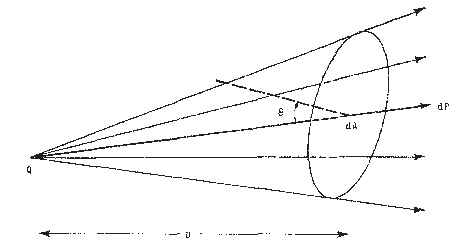
\includegraphics{figures/nicodemus1963-fig1.pdf}
\end{center}
\caption{An elementary pencil of radiation}
\label{fig:nicodemus1}
\end{figure}

In order to analyze this situation, let us first consider only the distribution
of power flow as a function of direction. We define an elementary pencil of rays
through a point $Q$ as including all of the rays which pass from $Q$ through an
element of area $dA$ at a distance $D$ from $Q$ which is very large in relation
to
the linear dimensions of $dA$ (see \cref{fig:nicodemus1}).
The solid angle subtended at $Q$ by $dA$ is given by
\begin{equation*}
\d\omega = \frac{\cos\theta \d A}{D^2}
\qquad \left[\unit{\steradian}\right],
\end{equation*}
where $\theta$ is the angle between the normal to $dA$ and the pencil of rays,
i.e., $\cos\theta\cdot dA$, is the projected area of $dA$ normal to this pencil.
If we next consider $Q$ not as a mathematical point, but as having dimensions
which, however, are very small compared to the dimensions of $dA$ (and, hence,
extremely small compared to $D$), the power which flows along the rays in this
pencil from $Q$ to $dA$ can be expressed as
\begin{equation*}
\d\Phi_e = I_e \d\omega = I_e \frac{\cos\theta \d A}{D^2}
\qquad \left[\unit{\watt}\right],
\end{equation*}
where
\begin{equation}
I_e \equiv \frac{\partial \Phi_e}{\partial \omega}
\qquad \left[\unit{\watt\per\steradian}\right]
\end{equation}
is defined as the \textsl{radiant intensity} (see \cref{tab:radiophoto}) of
$Q$ as a “point” source of radiation (e.g., a virtual source, such as the image
of an illuminated pin hole) \emph{in the direction of the pencil} (the direction of
$dA$ from $Q$). Note that $I_e$ may vary with direction and is a constant only
for an isotropic source. In general, the power received from a distant “point"
source is given by
\begin{equation}
\Phi_e = \int I_e \d\omega
\qquad \left[\unit{\watt}\right],
\end{equation}
where the integration is carried out over the entire solid angle subtended at
the source by the receiver.

For completeness, we also look briefly at the purely spatial variation, although
this quantity is more easily understood and is not so often a source of
difficulty
or misunderstanding. If we consider an element of surface $dA$, situated
anywhere
in a radiation field, the total amount of radiant power passing through it
(either
into it from a hemisphere, or out of it into a hemisphere) can be expressed as
\begin{equation*}
\d\Phi_e = E_e \d A \quad \textrm{or} \quad \d\Phi_e = M_e \d A
\qquad \left[\unit{\watt}\right],
\end{equation*}
where
\begin{equation}\label{eqn:nicodemus4}
E_e \equiv \frac{\partial \Phi_e}{\partial A}
\qquad \left[\unit{\watt\per\square\meter}\right]
\end{equation}
is the \textsl{irradiance} (see \cref{tab:radiophoto}), the surface density
of radiant power flowing into the surface at a point from a complete hemisphere
(or, sometimes, from a stated solid angle which is less than a hemisphere), and
where
\begin{equation}\label{eqn:nicodemus5}
M_e \equiv \frac{\partial \Phi_e}{\partial A}
\qquad \left[\unit{\watt\per\square\meter}\right]
\end{equation}
%page 372
is the \textsl{radiant emittance} (see \cref{tab:radiophoto}), the surface
density of radiant power flowing out of the surface at a point into a complete
hemisphere. Both of these quantities may vary from point to point over an
extended
surface, so that the total radiant power flowing into the surface of a receiver
is given by
\begin{equation}
\Phi_e = \int E_e \d A
\qquad \left[\unit{\watt}\right],
\end{equation}
and that flowing out of the surface of a source is given by
\begin{equation}
\Phi_e = \int M_e \d A
\qquad \left[\unit{\watt}\right],
\end{equation}
where the integration is carried out over the entire surface of interest in each case.

\begin{figure}
\begin{center}
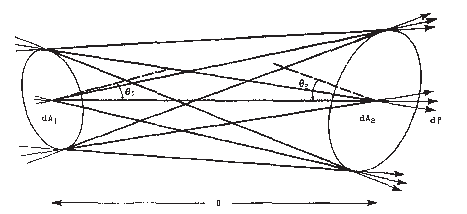
\includegraphics{figures/nicodemus1963-fig2.pdf}
\end{center}
\caption{An elementary beam of radiation between two surface elements $\d A_1$ and $\d A_2$}
\label{fig:nicodemus2}
\end{figure}

We now consider the simultaneous distribution of radiant flux in both space
and direction by examining an elementary beam of radiation. The elementary beam
of radiation between two elements of area $\d A_1$ and $\d A_2$, situated anywhere in
a radiation field where they are separated by a distance $D$ which is very large
compared to the linear dimensions of either element of area, is defined as
including
all of the rays which pass from $\d A_1$ to $\d A_2$ (or from $\d A_2$ to $\d A_1$, since either
may be the source and the other the receiver).
By inspection of \cref{fig:nicodemus2}, it can be seen that the cross
section of
the beam at either end is determined by the projected area of the element at
that end,
i.e., by $\cos\theta_1 \d A_1$ and $\cos\theta_2 \d A_2$, respectively. Also, the
solid angle
subtended at the opposite end by each element is equal to this projected area
divided by
$D^2$ in each case, giving
\begin{equation*}
\d \omega_1 = \frac{\cos\theta_1 \d A_1}{D^2}
\qquad \left[\unit{\steradian}\right]
\end{equation*}
and
\begin{equation}
\d \omega_2 = \frac{\cos\theta_2 \d A_2}{D^2}
\qquad \left[\unit{\steradian}\right].
\end{equation}

If we compute the projected-area-solid-angle-product (which has also been
referred
to as the ``throughput''\footnote{\label{note:nicodemus7} The term
``throughput'' appears
in the instruction manual issued by Block Associates, Inc., for an
interferometer
spectrometer. It is not known who originated the term or the precise way in
which
he would define it, but it appears to agree with the way in which it is used
here})
at each end we have
\begin{align*}
\d G_1 &= \cos\theta_1 \d A_1 \d \omega_2 = \cos\theta_1 \d A_1 \frac{\cos\theta_2
\d A_2}{D^2} \\
\d G_2 &= \cos\theta_2 \d A_2 \d \omega_1 = \cos\theta_2 \d A_2 \frac{\cos\theta_1
\d A_1}{D^2}
\end{align*}
But
\begin{equation}
\d G_1 = \d G_2 = \d G
\qquad \left[\unit{\square\meter\steradian}\right].
\end{equation}

Next, let us recall the definition of \textsl{radiance}, the power per unit
projected
area per unit solid angle at a point and in a particular direction, as
\begin{equation*}
L_e \equiv \frac{\partial^2 \Phi_e}{\partial\omega\;\cos\theta \partial A}
\qquad \left[\unit{\watt\per\square\meter\per\steradian}\right].
\end{equation*}

If the radiance at $\d A_1$ is $L_{e1}$ and that at $\d A_2$ is $L_{e2}$, the power
flowing
through each surface element is given, respectively, by
\begin{align}
\d \Phi_{e1} &= L_{e1} \cos\theta_1 \d A_1 d\omega_2 = L_{e1} \d G \nonumber\\
\d \Phi_{e2} &= L_{e2} \cos\theta_2 \d A_2 d\omega_1 = L_{e2} \d G.
\end{align}

But the same power is flowing through both of the surface elements that define
the
beam, since all rays through one also pass through the other and energy is
conserved
(we have postulated no loss), so
\begin{equation}
\d \Phi_{e1} = \d \Phi_{e2}\quad \textrm{and} \quad L_{e1} = L_{e2} = L_e.
\end{equation}

Since the choice of $\d A_1$ and $\d A_2$ is quite arbitrary, and they can define a
beam between any widely separated points along a particular ray, it follows that
\emph{the value of $L_e$ in the direction of a ray must be invariant along that
ray within an isotropic medium}.
The value of $L_e$ at any point will vary with direction, and the value of $L_e$
for rays from a particular direction (parallel rays) will vary with position on
any surface which they intersect. Hence, in general, the flux passing through a
given surface and within a given solid
%page 373
angle is given by
\begin{equation}\label{eqn:nicodemus12}
\Phi_e = \int \int L_e \cos\theta \d A \, \d \omega
\qquad \left[\unit{\watt}\right],
\end{equation}
where the integration is carried out over the entire surface (with respect to
the projected area perpendicular to any given direction) and over all directions
included within the given solid angle.

\begin{figure}
\begin{center}
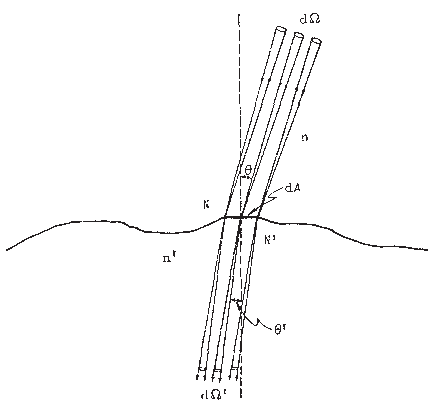
\includegraphics{figures/nicodemus1963-fig3.pdf}	
\end{center}
\caption{Refraction at a smooth boundary between media of
different refractive indices ($n$ and $n'$)}
\label{fig:nicodemus3}
\end{figure}

In order to generalize still further, we examine the situation where a beam of
radiation passes through a smooth surface separating two media with different
refractive indices (see \cref{fig:nicodemus3}). The power incident on any
surface element $\d A$ through any element of solid angle $\d \omega$ in the first
medium and that from the same beam emerging from the same surface element into
a solid angle $\d \omega'$ in the second medium must be the same, if there are no
losses by reflection, absorption, or scattering (we are still concerned purely
with ray geometry and defer questions of Fresnel reflection losses, etc., until
later). This power is given by
\begin{equation}\label{eqn:nicodemus13}
d\Phi_e = L_e\,\cos\theta \d A\, \d \omega = L_e'\,\cos\theta' \d A\, \d \omega'
\qquad \left[\unit{\watt}\right].
\end{equation}

By Snell's law of refraction, we write
\begin{align}
n\sin\theta &= n' \sin \theta' \\
\therefore\quad n\cos\theta \d \theta &= n' \cos\theta' \d \theta'.
\end{align}
Also,
\begin{equation}
\d\omega = \sin\theta\d\theta \d\phi
\quad \textrm{and} \quad
\d\omega' = \sin\theta'\d\theta' \d\phi
\end{equation}
(the azimuth angle $\phi$ of a ray is not changed by refraction). Hence,
\begin{equation*}
\frac{L_e \d A \cos\theta \d\omega}{L_e' \d A \cos\theta' \d\omega'} =
\frac{L_e \cos\theta \sin\theta \d\theta \d\phi}{L_e' \cos\theta' \sin\theta' \d\theta' \d\phi}
\frac{L_e n'^2}{L_e' n^2} = 1
\end{equation*}
\begin{equation}
\therefore\quad \frac{L_e}{n^2} = \frac{L_e'}{n'^2} \label{eqn:nicodemus17}
\end{equation}
Thus, \emph{the quantity $L / n^2$ in the direction of a ray is invariant along
that ray}, even as it passes through a smooth boundary surface between media of
different refractive indices, if there are no losses by reflection, absorption,
or scattering (see~\citerad[pp.
266--268]{martin60}\footnote{\label{note:nicodemus8__}Martin's proof is given
only for the luminance $L_v$ of an image, but with
only slight modification it, too, is easily generalized to apply to any
point along a ray.}). It is also apparent from \cref{eqn:nicodemus17}
that the value of $L_e$ in the direction of a ray will be the same at any
point along such a ray which lies in a medium with the same index, regardless
of passage through other media, such as refractive lenses, at intermediate
points.
Total reflection from a smooth surface merely changes the direction of a
beam and does not alter $L_e$. This can be verified in detail by an analysis
similar to that just given for refraction at a smooth boundary.

A “smooth” surface, as the term is used here, is defined to include any
surface where it is possible everywhere to construct a tangent plane,
i.e., where every surface element can be treated as common to the
surface and to a plane tangent to the surface at that point.

It should be recognized, of course, that all real situations involve
some losses by absorption, scattering, or reflection, although it is
frequently possible to keep the losses to negligible amounts
by careful design. Also, in real situations we are concerned with sources
and receivers, not hypothetical elements of surface.

In the foregoing analysis, we have attempted to achieve as much generality
as possible by considering radiation fields and surface elements placed in
those fields with as few restrictions as possible. In this way, the results
of the analysis can be extended widely to describe the radiometric quantities
at the surfaces of almost any receiver of radiation in terms of those quantities
at any source, or at any intermediate location where it may be convenient to specify or measure
%page374
them. This has been done purely in terms of ray geometry, neglecting losses
by absorption, scattering, and reflection. Such losses, where they are
not negligible, can be accounted for by multiplying the radiometric quantities,
determined from ray geometry only, by the appropriate factors.
For example, if the radiance along a particular ray at a source is
$L_{es}$, and the radiant transmittance (see \cref{tab:radiophoto}) along
its path (taking into account the source spectrum and the spectral transmittance
(see \cref{tab:radiophoto}) of the intervening medium) from source to
receiver is $\tau$, and source and receiver both lie in the same medium (same
index of refraction), then the radiance at the receiver in the direction of
this same ray is given by $L_{er} = \tau L_{es}$. If, in addition, this same
ray has also been imperfectly reflected by a mirror at some point along its
path to the receiver, the radiance at the receiver becomes $L_{er} = \rho \tau L_{es}$,
where $\rho$ is the radiant reflectance (see \cref{tab:radiophoto}) of
the mirror.

A situation of even more importance, perhaps, is the effect of reflection loss
on the radiance along a ray which is refracted at a boundary between two media
of different refractive indices.
Fresnel’s equations require that there be some reflectance at any simple
boundary between two such media. Here, if the radiance along the incident ray
is $L_e$, and if the radiant reflectance for the particular angle of incidence
is $\rho$, the radiance along the refracted ray in the second medium
will be given by
\begin{equation}
L'_e = L_e \frac{n'^2}{n^2} (1-\rho)
\qquad \left[\unit{\watt\per\square\meter\per\steradian}\right].
\end{equation}
Note, however, that it may be possible to reduce $\rho$ to a negligible value,
at least for a limited range of wavelengths and angles of incidence, by the
use of so-called antireflection coatings, thus approaching the condition
described by \cref{eqn:nicodemus17}.

\section{Practical applications}
[omitted---\textit{Ed.}]

\ifomit
Before describing some situations which illus-
trate the usefulness of the invariant property of
radiance, we consider briefly the limitations
governing the application of the concepts of
radiance and radiant intensity to real sources.
To look first at the extremes, it is obviously
meaningless, with respect to a receiver at the
earth’s surface, to speak of the radiance of a star
or the radiant intensity of a clear sky. Even the
nearest star, in spite of its huge size, subtends
such a small solid angle at the earth that it
defines a pencil, rather than a beam, of radiation.
Hence it is characterized by its radiant intensity.
Conversely, the sky subtends so large a solid
angle that, for most purposes it is necessary to
recognize the variations in its radiance in differ-
ent directions from a receiver at the ground.

Most sources fall into an intermediate category
where they may be characterized by their radi-
ance or their radiant intensity, depending on the
distance of the receiver and the size of the smal-
lest solid angle or resolution element which is
considered significant. Thus a planet, like a star,
will ordinarily define a pencil of radiation, i.e.,
its radiant intensity is the quantity of importance
in determining the total radiant power reaching
the aperture of a telescope on earth from the
entire planet. However, the amount of radiant
power in various portions of a highly magnified
image of the planet Mars, for example, is a func-
tion of the radiance of the corresponding portions
of the planet's surface in the direction of the
earth. Similarly, the plume of a large missile in
powered flight is clearly an extended source, with
a complicated spatial distribution of varying
radiance, with respect to a receiver at a distance
of a few hundred feet. However, from high alti-
tudes such a plume may be treated as a point
source, characterized by its radiant intensity in

FIG. 4. A simple radiom-
eter; A sensitive receiv-
er (detector) of area a
is located at one end of
an opaque tube of length
6 with an aperture of area
A in the opposite end of
the tube to limit the beam
of rays incident upon the
receiver.

% end of page

the direction of a detection device on the ground
in most i11sta11ces where the field of View of the
device is large enough to permit acquisition and
tracking of the moving target without unusually
complex and expensive equipment.
The 'L1sefu111ess of the invariant property of
radiance can be illustrated in connection with a
very simple radiometer consisting of a detector
with a flat sensitive surface of area a, such as a
common lead sulphide cell, mounted in a tube of
length 4?, with a limiting aperture of area at the
tar end to define the beam of radiation incident
on the detector (see Fig. 4). It is assumed that
the ratio of /5 to the linear dimensions of the
detector is large enough so that, to the desired
degree of accuracy, the detector subtends the
same solid angle Qza/£3 at all points of the
entrance aperture. It such an instrument is
placed close enough to an extended source of
uniform radiance _N, the total radiant power"
incident on the cell (measured by its electrical
response) can be written immediately as

P 2 rA7,in 3 viva a/.52 [W],

where T is the total radiant transmittance over
the path from source to cell. This is possible
because We know that, in the absence of loss, the
radiance along each ray at the entrance aperture
is N, the same as at the source along the same
rays. And at this position the rays fill an area A
and a solid angle Q=a/W at each point Within
that areal In practice, by measuring P from the
response of the cell, and knowing 7-, A, a, and -E,
we can compute the radiance of an unknown
imzform source as

P59
N z
7-A at

(19)

UN - c111‘? - sr‘l:]. (20)

ll 7 is unlrnovvn, as is frequently the case for
atmospheric transmittance, we will measure in-
stead the apparent radiance (at the radiometer)

Pr?
N’ 2 izrv rm

[VV ~ cm“? - sr‘1].
Au,

(21)

Probably, in a practical situation, the values of
ill, :1, and -ti, will not be determined individually.
Instead, the factor

rainzirra,/ezupd,/‘N’=Pft.iil’nv [Cassi] (22)

3 riELD srse
m-**“ j; (In rocit

Lriis inn PMNE)

APERTURE STU?

FIG. 5. Nearusmall-source (Jones method) calibration.
Source completely Within region bounded by XZ and YZ,
which make an angle 6 with the optical axis. 6=ha.lf-field
angle. P=arbit.rary point of source. Rays from any such
point P Within a cone of half-angle 8 will uniformly irradiate
the field stop as shown.

which has been called the “throughput,” will be
determined by a calibration measurement of a
source of known radiance at a distance Where 7
is known or is practically unity (negligible
attenuation).
Another illustration of useful application of
the general property of invariance, at points
Where rays do not cross to form an image of the
source, is in connection with the so-called Jones
Wethodg =10 for calibrating a radiometer. As shown
in Fig. 5, a small source (area small compared
with the area of the radiometer aperture) is
placed close to the radiometer Where it will uni-
formly irradiate the field stop of the instrument.
In order to do this, the source must be small
enough and close enough so that the radiometer
aperture subtends, at every point of the source,
an angle greater than the field angle of the in-
strument. As can be seen in Fig. 5, this means
that the source must lie entirely Within the region
enclosed by the cone represented by the lines
XZ and YZ, which meet at Z to form an angle
equal to the field angle of the radiometer, as
shown.
In the following approximate treatment, it is
assumed that the optics are ideal, so that a
parallel bundle of rays incident on the aperture
stop of the instrument is sharply focused at a

9 This method was first used by Dr. R. C. Jones in the
fall of 1951 on Navy Contract NObsr 42179. The method
became known by word of mouth, and was first described
in writing in “An Unusual Method for Calibrating an
Infrared Radiometer” (Polaroid Corporation, 19 Septem~
ber 1955, Memorandum 614) under Navy Contract
NOhsr 63175.
1° “The Jones Method of Radiometer Calibration” Tech»
mignes (Barnes Engineering Company, winter, 1957).
Reprints of this article have also been issued as Barnes
Engineering Infrared

% end of page

376

APERTURE

FIELD

FIG. 6. Alternative illustration of Jones method of calibra-
tion. P’ is an arbitrary point within the field stop.

single point lying in the field stop. Also, it is
assumed that the field angle is small so that for
the angle 0 shown in Fig. 5, coso'- 1.

Consider any point P on the radiating surface
of the source. It is apparent in Fig. 5 that the
rays emitted from P within a solid angle 9 equal
to the field angle of the radiometer will uniformly
irradiate the field stop. If the radiance of the
source is N5, and its projected area (normal to
the optic axis) is As, the total radiant power thus
radiated from all points of the source through the
field stop (in the absence of absorption, reflection,
and scattering losses) is given by

P = N.A.rz [W]. (23)

Alternatively, as illustrated in Fig. 6, we may
consider any point P’ within the field stop. All
rays reaching P’ from the source must travel
parallel to each other in a single direction from
the source to the radiometer aperture. There they
will fill an area of the aperture equal to AS, the
projected area of the source. They are then
focused onto P’. The effective aperture area As
subtends a solid angle at P’ given by

[Sr].

where F is the focal length of the radiometer
optics. Since the radiance at the field stop in the
direction of any of the rays from the source is
equal to the source radiance N3, we can write

[W].

where A F is the area of the field stop. Since the
field solid angle is given by

w%As/F2 (24)

P=N.A ,.~o.»=NsA FA./F2 (25)

s2=A F/F2 [Sr], (26)

FRED E. NICODEMUS

it can be seen that
P:-N..A_.A F/F2=N.A,S2 [W], (27)

in agreement with Eq. (23). Note that in this
case the source is not imaged at the field stop
where the value of radiant power P is being
evaluated.
\fi

\section{Discussion of introductory examples}

In the Introduction we described three situations involving extended sources.
It should be clear from \cref{eqn:nicodemus13} that the exposure meter must
give the same response, regardless of distance or orientation, as long as all
of the radiation entering it has the same value of radiance. If the wall
is perfectly diffuse, all of the rays from it will have the same radiance.
An external lens cannot change either the area or angle through which the
meter accepts radiation, whether it comes directly from the wall or after it
passes through the lens, and the value of radiance also cannot be changed
(except by attenuation, which is assumed negligible). In the same way, once
the full receiving area (entrance slit) and solid angle (subtended at the
slit by the collimating optics) of the spectrometer are filled with rays of
the maximum available radiance, there remains no way to increase any of these
quantities with additional lenses. In the last example, we must first determine
the radiance $L_e$ of the earth’s surface.
From \cref{eqn:nicodemus1} and \cref{eqn:nicodemus5} we can write
for a uniform plane diffuse radiator for which both $L_e$ and $M_e$ are constants:
\begin{equation*}
\Phi_e = \int M_e \d A = \int \int L_e \cos\theta \d A \d \omega
\qquad \left[\unit{\watt}\right],
\end{equation*}
\begin{equation}
\therefore\quad M_e = L_e \int \cos\theta \d \omega
\qquad \left[\unit{\watt\per\square\meter}\right],
\end{equation}
If we choose spherical coordinates with the $z$ axis perpendicular to the
radiating surface,
\begin{equation*}
\d \omega = \sin\theta\d\theta \d \phi
\qquad \left[\unit{\steradian}\right]
\end{equation*}
and
\begin{equation}
M_e = L_e \int_{\phi = 0}^{2\pi} \int_{\theta=0}^{\frac{\pi}{2}}\cos\theta
\sin\theta\d\theta \d\phi
= L_e \left.\phi\right|_{0}^{2\pi} \left.\frac{\sin^2\theta}{2}\right|_{\theta=0}^{\frac{\pi}{2}} = \pi L_e
\qquad \left[\unit{\watt\per\square\meter}\right].
\end{equation}
%page377
Similarly, from \cref{eqn:nicodemus1} and \cref{eqn:nicodemus4},
the irradiance at a plane surface due to uniform radiation of radiance $L_e$,
arriving within a cone of half-angle $\theta$, is given by
\begin{equation}
E_e = L_e \int \cos\theta \d\omega = \pi L_e \sin^2\theta
\qquad \left[\unit{\watt\per\square\meter}\right].
\end{equation}
This gives the desired result for an earth of uniform radiance
$L_e = M_e / \pi$ which subtends a cone of half-angle $\theta$ at the
receiver ($E_e = M_e \sin^2\theta$).

\section{Summary}

It has been established that in any radiation field radiance is invariant along
a ray, in the direction of the ray, within an isotropic medium, and that the
quantity $L_e/n^2$ is invariant along a ray, in the direction of the ray,
across smooth boundaries between media with different refractive indices,
so that $L_e$ has the same value at all points along the ray lying in media
of the same index, regardless of passage through other media at intermediate
points. Practical applications of the usefulness of this invariant property have
been presented. They show that it facilitates the evaluation of the radiant
power
flowing through any surface where it is possible to determine the cross section
of a beam (the projected area of its intersection with the surface) and the
solid
angle from which rays are flowing through each point of that surface, if the
value
of radiance is known at any point along each of the rays. In practical optical
systems,
such surfaces are usually found at the stops (aperture stop and field stop) and
their images (e.g., the entrance and exit pupils and windows), and at the
surfaces
of sources and receivers, and their images.

Evaluation of radiant power becomes a very simple matter for a beam passing
through
a well-defined plane surface ($\theta$ is not a function of position) of area
$A$
and within a well-defined solid angle $\omega$ that is the same at all points of
the
surface (no vignetting) whenever it is possible to assume a uniform value of
radiance
$L_e$ throughout the beam. The general expression in \cref{eqn:nicodemus12} can
then be simplified as follows:
\begin{equation}
\Phi_e = \int \int L_e \cos\theta \d A \d \omega = L_e A \int \int \cos\theta
\d \omega =
L_e A \Omega^\perp
\qquad \left[\unit{\watt}\right].
\end{equation}
The expression $\Omega^\perp = \int \int \cos\theta \d \omega$ has been called the
``weighted solid angle'' or ``projected solid angle''(see~\citerad{jones60}).
The area-solid-angle-product, ``optical invariant''
(see~\citerad{jones62a}\footnote{Although not flagged out, the concept of
invariance of the $A\Omega$ product is also used by R. Clark Jones in two other
papers: \citerad{jones53,jones62b}}), ``throughput''\cref{note:nicodemus7} or
``\'etendue'' (see~\citerad{connes58}\footnote{I am indebted to Dr. R. Clark
Jones for calling my attention to this reference}) can be given for the
unvignetted beam through a plane surface or aperture of area $A$ as
\begin{equation}
G = A\Omega^\perp = A \int \int \cos\theta \d \omega
\qquad \left[\unit{\square\meter\steradian}\right].
\end{equation}
Furthermore, in most cases the solid angle is a circular cone of
half-vertex-angle
$\theta$, with its axis perpendicular to the plane. Then, using spherical
coordinates
with the $z$ axis perpendicular to the plane, the integration can be carried out thus:
\begin{equation}
G = A\int_{\phi = 0}^{2\pi} \int_{\theta=0}^{\theta}\cos\theta \sin\theta\d\theta \d\phi
=\pi A \sin^2\theta
\qquad \left[\unit{\square\meter\steradian}\right].
\end{equation}
and
\begin{equation}
\Phi_e = L_e G = \pi L_e A \sin^2\theta
\end{equation}

\section{Acknowledgement}

In this report, the author has made extensive use of the ideas of others, gained
from many stimulating and helpful discussions and from published books and
papers, over an extended period. To attempt to list and acknowledge all of these
sources would be impossible, and it has not been attempted except in the few
instances where specific reference has been made to published items. However,
the development of this treatment of the subject would have been impossible
without such help and encouragement.

% put this bibliography as a section, numbered
\let\originalbibsection\bibsection
\renewcommand{\bibsection}{\section{\refname}}
\bibliographystylerad{plainnat}
\bibliographyrad{bibliography_radiance}
\let\bibsection\originalbibsection


% put this bibliography as a chapter
\bibliographystyle{plainnat}
\bibliography{bibliography}

%\printindex
%\indexprologue{This is a list of names}
%\printindex[persons]
\PrintGlossaries

\end{document}
